\documentclass[american,oneside]{ntnuthesis}
%\documentclass[american,titlepage,oneside]{ntnuthesis}

\usepackage{pdflscape}
\usepackage{layouts}
\usepackage{titling}
\usepackage{float}
\usepackage{svg}

%\usepgfplotslibrary{external}
%\tikzexternalize[prefix=figures/,optimize command away=\includepdf]


\pretitle{
    \begin{flushleft}
    \huge
}
\title{\textbf{Secure code synthesis}}
\posttitle{\end{flushleft}}
\shorttitle{Secure code synthesis}
\preauthor{\begin{flushleft}
    \vspace{2cm}\LARGE
}
\author{André Storhaug}
\postauthor{\par\end{flushleft}}
\shortauthor{A. Storhaug}
\predate{\begin{flushleft}\Large}
\date{\textbf{Spring 2022}\\
    \vfill\large Master of Science in Computer Science\\
    Supervisor: Jingyue Li - Associate Professor at NTNU\\
    \vspace{1cm}\large\textbf{NTNU}\\
    \normalsize Norwegian University of Science and Technology\\
    Faculty of Information Technology and Electrical Engineering\\
    Department of Computer Science
}
\postdate{\par\end{flushleft}}


\addbibresource{refs.bib}

\input{glossary.tex} % add glossary and acronym lists before document

\begin{document}

\includepdf[pages=-]{metadata/front-cover.pdf}

\chapter*{Abstract}

Writing \acrfullpl{sc} are hard. Writing secure \acrshortpl{sc} is even harder. Automatic code generation is by many considered the ”holy grail” in the field of computer science. Recent advances in transformer models have shown great potential in the area of synthesizing code from code comments. However, it is just as important \textit{how} these models are best put to use. In this thesis, it is investigated: how to automatically generate \acrlong{sc} code with transformer-based language models, by inputting comments to guide the code generation? Due to the monetary and immutable nature of blockchain, security in \acrshortpl{sc} is of uttermost importance. This thesis also investigates: how to generate secure \acrlong{sc} code with transformer-based language models? A design science research approach is adopted for answering these research questions. For automatically synthesizing \acrshort{sc} code, the 6 billion parameter model GPT-J by EleutherAI is fine-tuned on \acrshort{sc} code. For this task, the currently largest dataset of real \acrshort{sc} code is constructed, containing 186,397 contracts. To evaluate the comment-aid approach to generate code, the original code was used as the ground truth. This code was then compared with the generated code, and their differences were measured using the \acrfull{bleu} score. Results of the evaluation show that this approach results in a \acrshort{bleu} score of 0.557, which is beyond the state-of-the-art. For generating secure \acrlong{sc} code with transformer-based language models, a novel method named security conditioning is proposed. From both automatic and manual evaluation of the technique, the evaluation results show that security conditioning produced secure code.


%One sentence of
%- Your research motivation (argue why it is important to do your study)
%- List research questions 
%- Briefly explain the research methods
%- Summarize research results and main contributions (results and contributions should be linked to your research questions)
%
%To sell the idea and main results of your thesis





\chapter*{Sammendrag}
Aute culpa cillum elit non sunt mollit tempor dolore tempor excepteur. Pariatur nostrud consequat pariatur in officia commodo tempor consequat veniam in velit. Cupidatat adipisicing eiusmod sunt laboris ex deserunt ullamco laboris. Incididunt cillum dolor aute irure id cupidatat irure. Cillum nulla mollit incididunt commodo consectetur. Est cupidatat et excepteur non ad. Esse et Lorem dolor laboris sit velit incididunt dolor veniam pariatur est ad.
%This is the Acknowledgement
%%=========================================
\chapter*{Acknowledgement}
Nostrud est velit minim laborum amet nisi enim est aute cupidatat eu amet Lorem. Enim elit ipsum culpa cupidatat officia. Aliqua minim veniam consectetur anim occaecat nulla commodo aute aliqua. Esse excepteur ullamco adipisicing quis nisi. Enim reprehenderit ex quis velit qui nostrud. Magna commodo elit labore sunt deserunt nostrud et mollit consequat nulla. Pariatur irure ut elit qui sunt veniam enim culpa consectetur id est commodo eu.

\bigskip\noindent
This work is supported by the Research Council of Norway (No.309494).

%\bigskip
\begin{flushright}
    André Storhaug, Trondheim 28.05.2022
\end{flushright}

\tableofcontents
\listoffigures
\listoftables
\lstlistoflistings

\printglossary[type=\acronymtype] % Print acronyms
\printglossary                    % Print glossary
%\listoftodos

\chapter{Introduction}
\label{chap:introduction}
The art of computer programming is an ever-evolving field. The field has transformed from punchcards to writing assembly code. With the introduction of the C programming language, the field sky-rocketed. Since then, many new languages have been introduced, and the art of programming has become a complex and ever-changing field. Today, computer systems are all around us and permeate every aspect of our lives. However, constructing such systems is a hard and time-consuming task. Several tools and methods have been developed to increase the productivity of programmers, as well as to make programming more accessible to everyone. 

Recent advancements in large-scale transformer-based language models have successfully been used for generating code. Automatic code generation is a new and exciting technology that opens up a new world of possibilities for software developers. One example is GitHub Copilot \cite{copilot}. Copilot uses these models to generate code for a given programming language. The tool is based on a deep learning model, named Codex \cite{chen2021codex} by OpenAI, that has been trained on a large corpus of code. This enables developers to significantly speed up productivity. In addition, it makes programming more accessible to everyone by significantly reducing the threshold for using various programming languages and libraries. Another recent contribution is AlphaCode \cite{alphacode}, a code generation tool for generating novel code solutions to programming competitions.

The language models are getting larger and better by the day. However, it is just as important \textit{how} these models are best put to use. Describing functionality is easy. Implementing it in code is hard. Almost every coding language supports some form of code comment. These are normally created to explain the implemented code after the code is written. Recent works \cite{chen2021codex,colin2020pymt5} have leveraged the power of transformers to automatically generate code from comments. This has the potential to greatly lower the threshold for non-developers to leverage programming, while also increasing efficiency due to a simpler developing process. However, none of these works investigates how to best write these comments for guiding code generation. Further, for evaluating these systems, they only consider generating code from comments in isolation. This is rarely the case in a real-world setting because developers write code and use comments to explain the code. This thesis investigates a comment-aided approach to generating code, meaning the use of the existing code and comments as the input. For generating code, this work does not exclude the opportunity for developers to type in code and comments in combination with the automatically generated code. 

A machine learning model is only as good as the data it is fed. These large-scale transformers need huge amounts of data to be trained. Normally, this data is collected from all available open source code. A problem with this is that a lot of this code contains security problems. This can be everything from exposed API keys, to exploitable vulnerabilities. Autocomplete tools like GitHub Copilot must therefore be used with caution \cite{chen2021codex}.

To better secure automatic code generation, this thesis also purposes a novel approach for use of \acrshort{ml} models in large-scale transformer-based code generation pipelines to ensure secure generated code. To demonstrate the approach, this thesis will focus on generating secure code for \acrfullpl{sc} (Solidity). \acrfullpl{sc} have an exceptionally high demand for security, as vulnerabilities can not be fixed after a contract is deployed. Due to most blockchains' monetary and anonymous nature, they pose as a desirable target for adversaries and manipulators \cite{atzei2017survey}. Further, \acrshortpl{sc} tends to be rather short and simple, making it a good fit for generated code. The main research questions addressed in this thesis are:
\begin{itemize}
    \item How to automatically generate \acrlong{sc} code with transformer-based language models, by inputting comments to guide the code generation?
    \item How to generate secure \acrlong{sc} code with transformer-based language models?
\end{itemize}

\noindent
The specific contributions of this thesis are as follows:
\begin{itemize}
    \item The currently largest \acrfull{sc} dataset.
    \item Novel comment-aided code generation using the fine-tuned transformer-based language model to generate \acrlong{sc} code.
    \item Novel method to secure code generation.
    \item Identification of open issues, possible solutions to mitigate these issues, and future directions to advance the state of research in the domain.
\end{itemize}

The rest of this paper is organized as follows. \cref{chap:background} describes the background of the project. The research related to this document is commented in \cref{chap:related-work}. \cref{chap:research-methodoloy} describes the research methodology employed for implementing the research questions. The implementation and the results are presented in \cref{chap:implementation-and-results}. The implementations are then evaluated in \cref{chap:evaluation}. The findings and results from the implementation and evaluation are discussed in \cref{chap:discussion}. Finally, \cref{chap:conclusion} concludes the thesis, presenting final remarks and future works.

\chapter{Background}
\label{chap:background}
This chapter introduces the necessary background information for this study. First, an introduction to natural language processing is presented in \cref{sec:natural-language-processing}. Then, a thorough description of the Transformer model is provided in \cref{sec:transformer}. Following is \cref{sec:metrics}, explaining the different metrics used in this thesis. A brief introduction to blockchain technology is provided in \cref{sec:blockchain}. Then, the concept of \acrfullpl{sc} is introduced in \cref{sec:smart-contract}. Finally, in \cref{sec:smart-contract-vulnerabilities}, the most popular \acrshort{sc} vulnerabilities are described.

\section{Natural language processing}
\label{sec:natural-language-processing}
\todo{Used for comment clustering}

\subsection{Text preprocessing}
\label{sec:textt-preprocessing}
reducing capitalization, etc...
Stemming is the process of reducing a word to its word stem that affixes to suffixes and prefixes or to the roots of words known as a lemma. For example: words such as “Likes”, ”liked”, ”likely” and ”liking” will be reduced to “like” after stemming.

\subsection{Vector space model}
\label{sec:vector-space-model}

\subsubsection{Word2Vec}
\label{sec:vord2vec}
Or word embedding? as secttion.
https://ai.stackexchange.com/questions/26739/what-is-the-difference-between-a-language-model-and-a-word-embedding

Word Embeddings does not consider context, Language Models does.
For e.g Word2Vec, GloVe, or fastText, there exists one fixed vector per word.


The sentence:

Kill him, don't wait for me.

and

Don't kill him, wait for me.

If one averages the word embeddings, they would  produce the same vector. However,  in reality thheir meaning  (semantic) is very  diffferent.

\subsubsection{Term frequency-inverse document frequency}
\label{sec:tf-idf}

\section{Transformer}
\label{sec:transformer}
A transformer is a deep learning model. It is designed to process sequential data and adopts the mechanism of self-attention. The Transformer model architecture was introduced in \citeyear{vaswani2017attention} by \textcite{vaswani2017attention}. Unlike more traditional attention-based models such as \acrfullpl{rnn}, transformers do not include any recurrence or convolutions. This allows the model to process the entire input all at once, solely relying on attention. It solves the vanishing gradient problem of recurrent models, where long-range dependencies within the input are not accurately captured. It also allows the model to be significantly more parallelized, making training on huge datasets feasible. Because of this, pre-trained systems such as \acrfullpl{bert} and \acrshortpl{gpt} were developed. These models are pre-trained on a large corpus of text, such as Wikipedia Corpus and Common Crawl, and effectively predict the next word in a sentence. Further, the models can be fine-tuned on a new dataset to improve their performance on more specialized tasks.

\subsection{Attention}
\todo{Finish}
The self-attention mechanism is a mechanism that allows the model to learn to focus on a specific part of the input sequence. For example, cosider the following sentence: 
something somethin it..

By using the self-attention mechanism, the model can learn to focus on the word \textit{it} and ignore the other words. the context of the word \textit{it} is the word \textit{something} and \textit{something}. Hence, it is essential to know what \textit{it} refers to, in order to make a good prediction for the next word.

\cref{fig:attention-scores-example} shows the attention scores for the word \textit{it} in the sentence \textit{something something it..}.

\begin{figure}[htp]
    \centering
    \includegraphics[width=0.5\textwidth]{figures/attention-scores-example.png}
    \caption{TODO}
    \label{fig:attention-scores-example}
\end{figure}


\subsection{Architecture}
\label{sec:transformer-architecture}
The standard Transformer architecture, as describe by \citeyear{vaswani2017attention}, is shown in \cref{fig:transformer-architecture}. The following subsections describe the architecture of the standard Transformer model.

\begin{figure}[htp]
    \centering
    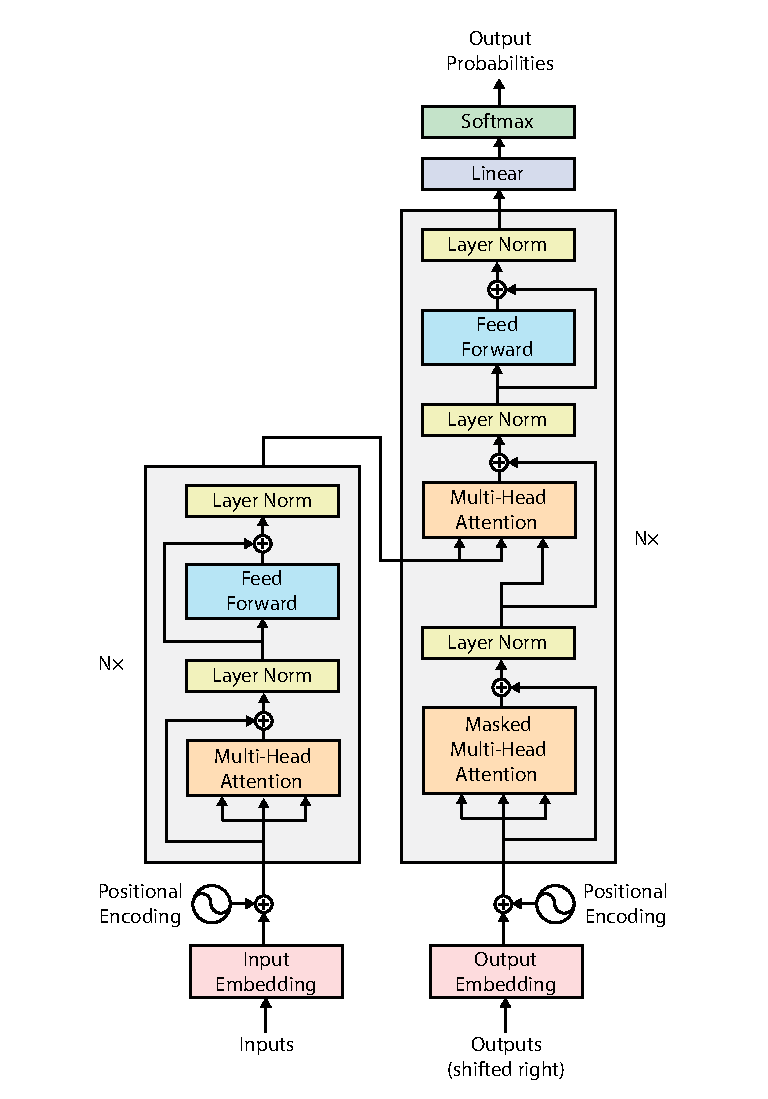
\includegraphics[width=0.8\textwidth]{figures/transformer_architecture.pdf}
    \caption{Architecture of a standard Transformer \textcite{vaswani2017attention}}
    \label{fig:transformer-architecture}
\end{figure}


\subsubsection{Tokenization}
\label{sec:tokenization}
For a Transformer to process the text input, the text is first tokenized. Tokenization is the process of breaking a sequence of text into a sequence of tokens. For example, the sentence \textit{I am a sentence.} is tokenized into the words \textit{I}, \textit{am}, \textit{a}, \textit{sentence}, and \textit{.}. The tokenization process is usually done by a tokenizer. Specifically, the transformer uses a byte pair encoding tokenizer.

\subsubsection{Embedding and Positional Encoding}
\label{sec:embedding-and-positional-encoding}
After the input text is tokenized, the next step for the model is to understand the meaning and position of the token (word) in the sequence. This is achieved by an Embedding layer and a Positional encoding layer. The results of these two layers are combined.

Two embedding layers are used. The Input Embedding layer is fed the input sequence. The Output Embedding layer accepts the target sequence after shifting the target to the right by one position and inserting a start token at the first position. The embedding layers produce a numerical representation of the input sequence, mapping each token to an embedding vector.

\begin{figure}[htp]
    \centering
    %% Creator: Matplotlib, PGF backend
%%
%% To include the figure in your LaTeX document, write
%%   \input{<filename>.pgf}
%%
%% Make sure the required packages are loaded in your preamble
%%   \usepackage{pgf}
%%
%% and, on pdftex
%%   \usepackage[utf8]{inputenc}\DeclareUnicodeCharacter{2212}{-}
%%
%% or, on luatex and xetex
%%   \usepackage{unicode-math}
%%
%% Figures using additional raster images can only be included by \input if
%% they are in the same directory as the main LaTeX file. For loading figures
%% from other directories you can use the `import` package
%%   \usepackage{import}
%%
%% and then include the figures with
%%   \import{<path to file>}{<filename>.pgf}
%%
%% Matplotlib used the following preamble
%%
\begingroup%
\makeatletter%
\begin{pgfpicture}%
\pgfpathrectangle{\pgfpointorigin}{\pgfqpoint{4.840359in}{2.401102in}}%
\pgfusepath{use as bounding box, clip}%
\begin{pgfscope}%
\pgfsetbuttcap%
\pgfsetmiterjoin%
\definecolor{currentfill}{rgb}{1.000000,1.000000,1.000000}%
\pgfsetfillcolor{currentfill}%
\pgfsetlinewidth{0.000000pt}%
\definecolor{currentstroke}{rgb}{1.000000,1.000000,1.000000}%
\pgfsetstrokecolor{currentstroke}%
\pgfsetdash{}{0pt}%
\pgfpathmoveto{\pgfqpoint{0.000000in}{-0.000000in}}%
\pgfpathlineto{\pgfqpoint{4.840359in}{-0.000000in}}%
\pgfpathlineto{\pgfqpoint{4.840359in}{2.401102in}}%
\pgfpathlineto{\pgfqpoint{0.000000in}{2.401102in}}%
\pgfpathclose%
\pgfusepath{fill}%
\end{pgfscope}%
\begin{pgfscope}%
\pgfsetbuttcap%
\pgfsetmiterjoin%
\definecolor{currentfill}{rgb}{1.000000,1.000000,1.000000}%
\pgfsetfillcolor{currentfill}%
\pgfsetlinewidth{0.000000pt}%
\definecolor{currentstroke}{rgb}{0.000000,0.000000,0.000000}%
\pgfsetstrokecolor{currentstroke}%
\pgfsetstrokeopacity{0.000000}%
\pgfsetdash{}{0pt}%
\pgfpathmoveto{\pgfqpoint{0.584568in}{0.499691in}}%
\pgfpathlineto{\pgfqpoint{4.053193in}{0.499691in}}%
\pgfpathlineto{\pgfqpoint{4.053193in}{2.252877in}}%
\pgfpathlineto{\pgfqpoint{0.584568in}{2.252877in}}%
\pgfpathclose%
\pgfusepath{fill}%
\end{pgfscope}%
\begin{pgfscope}%
\pgfsys@transformshift{0.584167in}{0.500269in}%
\pgftext[left,bottom]{\includegraphics[interpolate=true,width=3.469167in,height=1.752500in]{figures/positional_embedding-img0.png}}%
\end{pgfscope}%
\begin{pgfscope}%
\pgfsetbuttcap%
\pgfsetroundjoin%
\definecolor{currentfill}{rgb}{0.000000,0.000000,0.000000}%
\pgfsetfillcolor{currentfill}%
\pgfsetlinewidth{0.803000pt}%
\definecolor{currentstroke}{rgb}{0.000000,0.000000,0.000000}%
\pgfsetstrokecolor{currentstroke}%
\pgfsetdash{}{0pt}%
\pgfsys@defobject{currentmarker}{\pgfqpoint{0.000000in}{-0.048611in}}{\pgfqpoint{0.000000in}{0.000000in}}{%
\pgfpathmoveto{\pgfqpoint{0.000000in}{0.000000in}}%
\pgfpathlineto{\pgfqpoint{0.000000in}{-0.048611in}}%
\pgfusepath{stroke,fill}%
}%
\begin{pgfscope}%
\pgfsys@transformshift{0.584568in}{0.499691in}%
\pgfsys@useobject{currentmarker}{}%
\end{pgfscope}%
\end{pgfscope}%
\begin{pgfscope}%
\definecolor{textcolor}{rgb}{0.000000,0.000000,0.000000}%
\pgfsetstrokecolor{textcolor}%
\pgfsetfillcolor{textcolor}%
\pgftext[x=0.584568in,y=0.402469in,,top]{\color{textcolor}\rmfamily\fontsize{10.000000}{12.000000}\selectfont \(\displaystyle {0}\)}%
\end{pgfscope}%
\begin{pgfscope}%
\pgfsetbuttcap%
\pgfsetroundjoin%
\definecolor{currentfill}{rgb}{0.000000,0.000000,0.000000}%
\pgfsetfillcolor{currentfill}%
\pgfsetlinewidth{0.803000pt}%
\definecolor{currentstroke}{rgb}{0.000000,0.000000,0.000000}%
\pgfsetstrokecolor{currentstroke}%
\pgfsetdash{}{0pt}%
\pgfsys@defobject{currentmarker}{\pgfqpoint{0.000000in}{-0.048611in}}{\pgfqpoint{0.000000in}{0.000000in}}{%
\pgfpathmoveto{\pgfqpoint{0.000000in}{0.000000in}}%
\pgfpathlineto{\pgfqpoint{0.000000in}{-0.048611in}}%
\pgfusepath{stroke,fill}%
}%
\begin{pgfscope}%
\pgfsys@transformshift{1.126541in}{0.499691in}%
\pgfsys@useobject{currentmarker}{}%
\end{pgfscope}%
\end{pgfscope}%
\begin{pgfscope}%
\definecolor{textcolor}{rgb}{0.000000,0.000000,0.000000}%
\pgfsetstrokecolor{textcolor}%
\pgfsetfillcolor{textcolor}%
\pgftext[x=1.126541in,y=0.402469in,,top]{\color{textcolor}\rmfamily\fontsize{10.000000}{12.000000}\selectfont \(\displaystyle {10}\)}%
\end{pgfscope}%
\begin{pgfscope}%
\pgfsetbuttcap%
\pgfsetroundjoin%
\definecolor{currentfill}{rgb}{0.000000,0.000000,0.000000}%
\pgfsetfillcolor{currentfill}%
\pgfsetlinewidth{0.803000pt}%
\definecolor{currentstroke}{rgb}{0.000000,0.000000,0.000000}%
\pgfsetstrokecolor{currentstroke}%
\pgfsetdash{}{0pt}%
\pgfsys@defobject{currentmarker}{\pgfqpoint{0.000000in}{-0.048611in}}{\pgfqpoint{0.000000in}{0.000000in}}{%
\pgfpathmoveto{\pgfqpoint{0.000000in}{0.000000in}}%
\pgfpathlineto{\pgfqpoint{0.000000in}{-0.048611in}}%
\pgfusepath{stroke,fill}%
}%
\begin{pgfscope}%
\pgfsys@transformshift{1.668514in}{0.499691in}%
\pgfsys@useobject{currentmarker}{}%
\end{pgfscope}%
\end{pgfscope}%
\begin{pgfscope}%
\definecolor{textcolor}{rgb}{0.000000,0.000000,0.000000}%
\pgfsetstrokecolor{textcolor}%
\pgfsetfillcolor{textcolor}%
\pgftext[x=1.668514in,y=0.402469in,,top]{\color{textcolor}\rmfamily\fontsize{10.000000}{12.000000}\selectfont \(\displaystyle {20}\)}%
\end{pgfscope}%
\begin{pgfscope}%
\pgfsetbuttcap%
\pgfsetroundjoin%
\definecolor{currentfill}{rgb}{0.000000,0.000000,0.000000}%
\pgfsetfillcolor{currentfill}%
\pgfsetlinewidth{0.803000pt}%
\definecolor{currentstroke}{rgb}{0.000000,0.000000,0.000000}%
\pgfsetstrokecolor{currentstroke}%
\pgfsetdash{}{0pt}%
\pgfsys@defobject{currentmarker}{\pgfqpoint{0.000000in}{-0.048611in}}{\pgfqpoint{0.000000in}{0.000000in}}{%
\pgfpathmoveto{\pgfqpoint{0.000000in}{0.000000in}}%
\pgfpathlineto{\pgfqpoint{0.000000in}{-0.048611in}}%
\pgfusepath{stroke,fill}%
}%
\begin{pgfscope}%
\pgfsys@transformshift{2.210486in}{0.499691in}%
\pgfsys@useobject{currentmarker}{}%
\end{pgfscope}%
\end{pgfscope}%
\begin{pgfscope}%
\definecolor{textcolor}{rgb}{0.000000,0.000000,0.000000}%
\pgfsetstrokecolor{textcolor}%
\pgfsetfillcolor{textcolor}%
\pgftext[x=2.210486in,y=0.402469in,,top]{\color{textcolor}\rmfamily\fontsize{10.000000}{12.000000}\selectfont \(\displaystyle {30}\)}%
\end{pgfscope}%
\begin{pgfscope}%
\pgfsetbuttcap%
\pgfsetroundjoin%
\definecolor{currentfill}{rgb}{0.000000,0.000000,0.000000}%
\pgfsetfillcolor{currentfill}%
\pgfsetlinewidth{0.803000pt}%
\definecolor{currentstroke}{rgb}{0.000000,0.000000,0.000000}%
\pgfsetstrokecolor{currentstroke}%
\pgfsetdash{}{0pt}%
\pgfsys@defobject{currentmarker}{\pgfqpoint{0.000000in}{-0.048611in}}{\pgfqpoint{0.000000in}{0.000000in}}{%
\pgfpathmoveto{\pgfqpoint{0.000000in}{0.000000in}}%
\pgfpathlineto{\pgfqpoint{0.000000in}{-0.048611in}}%
\pgfusepath{stroke,fill}%
}%
\begin{pgfscope}%
\pgfsys@transformshift{2.752459in}{0.499691in}%
\pgfsys@useobject{currentmarker}{}%
\end{pgfscope}%
\end{pgfscope}%
\begin{pgfscope}%
\definecolor{textcolor}{rgb}{0.000000,0.000000,0.000000}%
\pgfsetstrokecolor{textcolor}%
\pgfsetfillcolor{textcolor}%
\pgftext[x=2.752459in,y=0.402469in,,top]{\color{textcolor}\rmfamily\fontsize{10.000000}{12.000000}\selectfont \(\displaystyle {40}\)}%
\end{pgfscope}%
\begin{pgfscope}%
\pgfsetbuttcap%
\pgfsetroundjoin%
\definecolor{currentfill}{rgb}{0.000000,0.000000,0.000000}%
\pgfsetfillcolor{currentfill}%
\pgfsetlinewidth{0.803000pt}%
\definecolor{currentstroke}{rgb}{0.000000,0.000000,0.000000}%
\pgfsetstrokecolor{currentstroke}%
\pgfsetdash{}{0pt}%
\pgfsys@defobject{currentmarker}{\pgfqpoint{0.000000in}{-0.048611in}}{\pgfqpoint{0.000000in}{0.000000in}}{%
\pgfpathmoveto{\pgfqpoint{0.000000in}{0.000000in}}%
\pgfpathlineto{\pgfqpoint{0.000000in}{-0.048611in}}%
\pgfusepath{stroke,fill}%
}%
\begin{pgfscope}%
\pgfsys@transformshift{3.294432in}{0.499691in}%
\pgfsys@useobject{currentmarker}{}%
\end{pgfscope}%
\end{pgfscope}%
\begin{pgfscope}%
\definecolor{textcolor}{rgb}{0.000000,0.000000,0.000000}%
\pgfsetstrokecolor{textcolor}%
\pgfsetfillcolor{textcolor}%
\pgftext[x=3.294432in,y=0.402469in,,top]{\color{textcolor}\rmfamily\fontsize{10.000000}{12.000000}\selectfont \(\displaystyle {50}\)}%
\end{pgfscope}%
\begin{pgfscope}%
\pgfsetbuttcap%
\pgfsetroundjoin%
\definecolor{currentfill}{rgb}{0.000000,0.000000,0.000000}%
\pgfsetfillcolor{currentfill}%
\pgfsetlinewidth{0.803000pt}%
\definecolor{currentstroke}{rgb}{0.000000,0.000000,0.000000}%
\pgfsetstrokecolor{currentstroke}%
\pgfsetdash{}{0pt}%
\pgfsys@defobject{currentmarker}{\pgfqpoint{0.000000in}{-0.048611in}}{\pgfqpoint{0.000000in}{0.000000in}}{%
\pgfpathmoveto{\pgfqpoint{0.000000in}{0.000000in}}%
\pgfpathlineto{\pgfqpoint{0.000000in}{-0.048611in}}%
\pgfusepath{stroke,fill}%
}%
\begin{pgfscope}%
\pgfsys@transformshift{3.836404in}{0.499691in}%
\pgfsys@useobject{currentmarker}{}%
\end{pgfscope}%
\end{pgfscope}%
\begin{pgfscope}%
\definecolor{textcolor}{rgb}{0.000000,0.000000,0.000000}%
\pgfsetstrokecolor{textcolor}%
\pgfsetfillcolor{textcolor}%
\pgftext[x=3.836404in,y=0.402469in,,top]{\color{textcolor}\rmfamily\fontsize{10.000000}{12.000000}\selectfont \(\displaystyle {60}\)}%
\end{pgfscope}%
\begin{pgfscope}%
\definecolor{textcolor}{rgb}{0.000000,0.000000,0.000000}%
\pgfsetstrokecolor{textcolor}%
\pgfsetfillcolor{textcolor}%
\pgftext[x=2.318881in,y=0.223457in,,top]{\color{textcolor}\rmfamily\fontsize{10.000000}{12.000000}\selectfont Depth}%
\end{pgfscope}%
\begin{pgfscope}%
\pgfsetbuttcap%
\pgfsetroundjoin%
\definecolor{currentfill}{rgb}{0.000000,0.000000,0.000000}%
\pgfsetfillcolor{currentfill}%
\pgfsetlinewidth{0.803000pt}%
\definecolor{currentstroke}{rgb}{0.000000,0.000000,0.000000}%
\pgfsetstrokecolor{currentstroke}%
\pgfsetdash{}{0pt}%
\pgfsys@defobject{currentmarker}{\pgfqpoint{-0.048611in}{0.000000in}}{\pgfqpoint{0.000000in}{0.000000in}}{%
\pgfpathmoveto{\pgfqpoint{0.000000in}{0.000000in}}%
\pgfpathlineto{\pgfqpoint{-0.048611in}{0.000000in}}%
\pgfusepath{stroke,fill}%
}%
\begin{pgfscope}%
\pgfsys@transformshift{0.584568in}{0.499691in}%
\pgfsys@useobject{currentmarker}{}%
\end{pgfscope}%
\end{pgfscope}%
\begin{pgfscope}%
\definecolor{textcolor}{rgb}{0.000000,0.000000,0.000000}%
\pgfsetstrokecolor{textcolor}%
\pgfsetfillcolor{textcolor}%
\pgftext[x=0.417902in, y=0.451466in, left, base]{\color{textcolor}\rmfamily\fontsize{10.000000}{12.000000}\selectfont \(\displaystyle {0}\)}%
\end{pgfscope}%
\begin{pgfscope}%
\pgfsetbuttcap%
\pgfsetroundjoin%
\definecolor{currentfill}{rgb}{0.000000,0.000000,0.000000}%
\pgfsetfillcolor{currentfill}%
\pgfsetlinewidth{0.803000pt}%
\definecolor{currentstroke}{rgb}{0.000000,0.000000,0.000000}%
\pgfsetstrokecolor{currentstroke}%
\pgfsetdash{}{0pt}%
\pgfsys@defobject{currentmarker}{\pgfqpoint{-0.048611in}{0.000000in}}{\pgfqpoint{0.000000in}{0.000000in}}{%
\pgfpathmoveto{\pgfqpoint{0.000000in}{0.000000in}}%
\pgfpathlineto{\pgfqpoint{-0.048611in}{0.000000in}}%
\pgfusepath{stroke,fill}%
}%
\begin{pgfscope}%
\pgfsys@transformshift{0.584568in}{0.842110in}%
\pgfsys@useobject{currentmarker}{}%
\end{pgfscope}%
\end{pgfscope}%
\begin{pgfscope}%
\definecolor{textcolor}{rgb}{0.000000,0.000000,0.000000}%
\pgfsetstrokecolor{textcolor}%
\pgfsetfillcolor{textcolor}%
\pgftext[x=0.279012in, y=0.793885in, left, base]{\color{textcolor}\rmfamily\fontsize{10.000000}{12.000000}\selectfont \(\displaystyle {100}\)}%
\end{pgfscope}%
\begin{pgfscope}%
\pgfsetbuttcap%
\pgfsetroundjoin%
\definecolor{currentfill}{rgb}{0.000000,0.000000,0.000000}%
\pgfsetfillcolor{currentfill}%
\pgfsetlinewidth{0.803000pt}%
\definecolor{currentstroke}{rgb}{0.000000,0.000000,0.000000}%
\pgfsetstrokecolor{currentstroke}%
\pgfsetdash{}{0pt}%
\pgfsys@defobject{currentmarker}{\pgfqpoint{-0.048611in}{0.000000in}}{\pgfqpoint{0.000000in}{0.000000in}}{%
\pgfpathmoveto{\pgfqpoint{0.000000in}{0.000000in}}%
\pgfpathlineto{\pgfqpoint{-0.048611in}{0.000000in}}%
\pgfusepath{stroke,fill}%
}%
\begin{pgfscope}%
\pgfsys@transformshift{0.584568in}{1.184529in}%
\pgfsys@useobject{currentmarker}{}%
\end{pgfscope}%
\end{pgfscope}%
\begin{pgfscope}%
\definecolor{textcolor}{rgb}{0.000000,0.000000,0.000000}%
\pgfsetstrokecolor{textcolor}%
\pgfsetfillcolor{textcolor}%
\pgftext[x=0.279012in, y=1.136304in, left, base]{\color{textcolor}\rmfamily\fontsize{10.000000}{12.000000}\selectfont \(\displaystyle {200}\)}%
\end{pgfscope}%
\begin{pgfscope}%
\pgfsetbuttcap%
\pgfsetroundjoin%
\definecolor{currentfill}{rgb}{0.000000,0.000000,0.000000}%
\pgfsetfillcolor{currentfill}%
\pgfsetlinewidth{0.803000pt}%
\definecolor{currentstroke}{rgb}{0.000000,0.000000,0.000000}%
\pgfsetstrokecolor{currentstroke}%
\pgfsetdash{}{0pt}%
\pgfsys@defobject{currentmarker}{\pgfqpoint{-0.048611in}{0.000000in}}{\pgfqpoint{0.000000in}{0.000000in}}{%
\pgfpathmoveto{\pgfqpoint{0.000000in}{0.000000in}}%
\pgfpathlineto{\pgfqpoint{-0.048611in}{0.000000in}}%
\pgfusepath{stroke,fill}%
}%
\begin{pgfscope}%
\pgfsys@transformshift{0.584568in}{1.526949in}%
\pgfsys@useobject{currentmarker}{}%
\end{pgfscope}%
\end{pgfscope}%
\begin{pgfscope}%
\definecolor{textcolor}{rgb}{0.000000,0.000000,0.000000}%
\pgfsetstrokecolor{textcolor}%
\pgfsetfillcolor{textcolor}%
\pgftext[x=0.279012in, y=1.478723in, left, base]{\color{textcolor}\rmfamily\fontsize{10.000000}{12.000000}\selectfont \(\displaystyle {300}\)}%
\end{pgfscope}%
\begin{pgfscope}%
\pgfsetbuttcap%
\pgfsetroundjoin%
\definecolor{currentfill}{rgb}{0.000000,0.000000,0.000000}%
\pgfsetfillcolor{currentfill}%
\pgfsetlinewidth{0.803000pt}%
\definecolor{currentstroke}{rgb}{0.000000,0.000000,0.000000}%
\pgfsetstrokecolor{currentstroke}%
\pgfsetdash{}{0pt}%
\pgfsys@defobject{currentmarker}{\pgfqpoint{-0.048611in}{0.000000in}}{\pgfqpoint{0.000000in}{0.000000in}}{%
\pgfpathmoveto{\pgfqpoint{0.000000in}{0.000000in}}%
\pgfpathlineto{\pgfqpoint{-0.048611in}{0.000000in}}%
\pgfusepath{stroke,fill}%
}%
\begin{pgfscope}%
\pgfsys@transformshift{0.584568in}{1.869368in}%
\pgfsys@useobject{currentmarker}{}%
\end{pgfscope}%
\end{pgfscope}%
\begin{pgfscope}%
\definecolor{textcolor}{rgb}{0.000000,0.000000,0.000000}%
\pgfsetstrokecolor{textcolor}%
\pgfsetfillcolor{textcolor}%
\pgftext[x=0.279012in, y=1.821142in, left, base]{\color{textcolor}\rmfamily\fontsize{10.000000}{12.000000}\selectfont \(\displaystyle {400}\)}%
\end{pgfscope}%
\begin{pgfscope}%
\pgfsetbuttcap%
\pgfsetroundjoin%
\definecolor{currentfill}{rgb}{0.000000,0.000000,0.000000}%
\pgfsetfillcolor{currentfill}%
\pgfsetlinewidth{0.803000pt}%
\definecolor{currentstroke}{rgb}{0.000000,0.000000,0.000000}%
\pgfsetstrokecolor{currentstroke}%
\pgfsetdash{}{0pt}%
\pgfsys@defobject{currentmarker}{\pgfqpoint{-0.048611in}{0.000000in}}{\pgfqpoint{0.000000in}{0.000000in}}{%
\pgfpathmoveto{\pgfqpoint{0.000000in}{0.000000in}}%
\pgfpathlineto{\pgfqpoint{-0.048611in}{0.000000in}}%
\pgfusepath{stroke,fill}%
}%
\begin{pgfscope}%
\pgfsys@transformshift{0.584568in}{2.211787in}%
\pgfsys@useobject{currentmarker}{}%
\end{pgfscope}%
\end{pgfscope}%
\begin{pgfscope}%
\definecolor{textcolor}{rgb}{0.000000,0.000000,0.000000}%
\pgfsetstrokecolor{textcolor}%
\pgfsetfillcolor{textcolor}%
\pgftext[x=0.279012in, y=2.163562in, left, base]{\color{textcolor}\rmfamily\fontsize{10.000000}{12.000000}\selectfont \(\displaystyle {500}\)}%
\end{pgfscope}%
\begin{pgfscope}%
\definecolor{textcolor}{rgb}{0.000000,0.000000,0.000000}%
\pgfsetstrokecolor{textcolor}%
\pgfsetfillcolor{textcolor}%
\pgftext[x=0.223457in,y=1.376284in,,bottom,rotate=90.000000]{\color{textcolor}\rmfamily\fontsize{10.000000}{12.000000}\selectfont Position}%
\end{pgfscope}%
\begin{pgfscope}%
\pgfsetrectcap%
\pgfsetmiterjoin%
\pgfsetlinewidth{0.803000pt}%
\definecolor{currentstroke}{rgb}{0.000000,0.000000,0.000000}%
\pgfsetstrokecolor{currentstroke}%
\pgfsetdash{}{0pt}%
\pgfpathmoveto{\pgfqpoint{0.584568in}{0.499691in}}%
\pgfpathlineto{\pgfqpoint{0.584568in}{2.252877in}}%
\pgfusepath{stroke}%
\end{pgfscope}%
\begin{pgfscope}%
\pgfsetrectcap%
\pgfsetmiterjoin%
\pgfsetlinewidth{0.803000pt}%
\definecolor{currentstroke}{rgb}{0.000000,0.000000,0.000000}%
\pgfsetstrokecolor{currentstroke}%
\pgfsetdash{}{0pt}%
\pgfpathmoveto{\pgfqpoint{4.053193in}{0.499691in}}%
\pgfpathlineto{\pgfqpoint{4.053193in}{2.252877in}}%
\pgfusepath{stroke}%
\end{pgfscope}%
\begin{pgfscope}%
\pgfsetrectcap%
\pgfsetmiterjoin%
\pgfsetlinewidth{0.803000pt}%
\definecolor{currentstroke}{rgb}{0.000000,0.000000,0.000000}%
\pgfsetstrokecolor{currentstroke}%
\pgfsetdash{}{0pt}%
\pgfpathmoveto{\pgfqpoint{0.584568in}{0.499691in}}%
\pgfpathlineto{\pgfqpoint{4.053193in}{0.499691in}}%
\pgfusepath{stroke}%
\end{pgfscope}%
\begin{pgfscope}%
\pgfsetrectcap%
\pgfsetmiterjoin%
\pgfsetlinewidth{0.803000pt}%
\definecolor{currentstroke}{rgb}{0.000000,0.000000,0.000000}%
\pgfsetstrokecolor{currentstroke}%
\pgfsetdash{}{0pt}%
\pgfpathmoveto{\pgfqpoint{0.584568in}{2.252877in}}%
\pgfpathlineto{\pgfqpoint{4.053193in}{2.252877in}}%
\pgfusepath{stroke}%
\end{pgfscope}%
\begin{pgfscope}%
\pgfpathrectangle{\pgfqpoint{4.269982in}{0.499691in}}{\pgfqpoint{0.087659in}{1.753186in}}%
\pgfusepath{clip}%
\pgfsetbuttcap%
\pgfsetmiterjoin%
\definecolor{currentfill}{rgb}{1.000000,1.000000,1.000000}%
\pgfsetfillcolor{currentfill}%
\pgfsetlinewidth{0.010037pt}%
\definecolor{currentstroke}{rgb}{1.000000,1.000000,1.000000}%
\pgfsetstrokecolor{currentstroke}%
\pgfsetdash{}{0pt}%
\pgfpathmoveto{\pgfqpoint{4.269982in}{0.499691in}}%
\pgfpathlineto{\pgfqpoint{4.269982in}{0.506539in}}%
\pgfpathlineto{\pgfqpoint{4.269982in}{2.246029in}}%
\pgfpathlineto{\pgfqpoint{4.269982in}{2.252877in}}%
\pgfpathlineto{\pgfqpoint{4.357642in}{2.252877in}}%
\pgfpathlineto{\pgfqpoint{4.357642in}{2.246029in}}%
\pgfpathlineto{\pgfqpoint{4.357642in}{0.506539in}}%
\pgfpathlineto{\pgfqpoint{4.357642in}{0.499691in}}%
\pgfpathclose%
\pgfusepath{stroke,fill}%
\end{pgfscope}%
\begin{pgfscope}%
\pgfsys@transformshift{4.270000in}{0.500269in}%
\pgftext[left,bottom]{\includegraphics[interpolate=true,width=0.087500in,height=1.752500in]{figures/positional_embedding-img1.png}}%
\end{pgfscope}%
\begin{pgfscope}%
\pgfsetbuttcap%
\pgfsetroundjoin%
\definecolor{currentfill}{rgb}{0.000000,0.000000,0.000000}%
\pgfsetfillcolor{currentfill}%
\pgfsetlinewidth{0.803000pt}%
\definecolor{currentstroke}{rgb}{0.000000,0.000000,0.000000}%
\pgfsetstrokecolor{currentstroke}%
\pgfsetdash{}{0pt}%
\pgfsys@defobject{currentmarker}{\pgfqpoint{0.000000in}{0.000000in}}{\pgfqpoint{0.048611in}{0.000000in}}{%
\pgfpathmoveto{\pgfqpoint{0.000000in}{0.000000in}}%
\pgfpathlineto{\pgfqpoint{0.048611in}{0.000000in}}%
\pgfusepath{stroke,fill}%
}%
\begin{pgfscope}%
\pgfsys@transformshift{4.357642in}{0.499691in}%
\pgfsys@useobject{currentmarker}{}%
\end{pgfscope}%
\end{pgfscope}%
\begin{pgfscope}%
\definecolor{textcolor}{rgb}{0.000000,0.000000,0.000000}%
\pgfsetstrokecolor{textcolor}%
\pgfsetfillcolor{textcolor}%
\pgftext[x=4.454864in, y=0.451466in, left, base]{\color{textcolor}\rmfamily\fontsize{10.000000}{12.000000}\selectfont \(\displaystyle {-1.0}\)}%
\end{pgfscope}%
\begin{pgfscope}%
\pgfsetbuttcap%
\pgfsetroundjoin%
\definecolor{currentfill}{rgb}{0.000000,0.000000,0.000000}%
\pgfsetfillcolor{currentfill}%
\pgfsetlinewidth{0.803000pt}%
\definecolor{currentstroke}{rgb}{0.000000,0.000000,0.000000}%
\pgfsetstrokecolor{currentstroke}%
\pgfsetdash{}{0pt}%
\pgfsys@defobject{currentmarker}{\pgfqpoint{0.000000in}{0.000000in}}{\pgfqpoint{0.048611in}{0.000000in}}{%
\pgfpathmoveto{\pgfqpoint{0.000000in}{0.000000in}}%
\pgfpathlineto{\pgfqpoint{0.048611in}{0.000000in}}%
\pgfusepath{stroke,fill}%
}%
\begin{pgfscope}%
\pgfsys@transformshift{4.357642in}{0.937988in}%
\pgfsys@useobject{currentmarker}{}%
\end{pgfscope}%
\end{pgfscope}%
\begin{pgfscope}%
\definecolor{textcolor}{rgb}{0.000000,0.000000,0.000000}%
\pgfsetstrokecolor{textcolor}%
\pgfsetfillcolor{textcolor}%
\pgftext[x=4.454864in, y=0.889762in, left, base]{\color{textcolor}\rmfamily\fontsize{10.000000}{12.000000}\selectfont \(\displaystyle {-0.5}\)}%
\end{pgfscope}%
\begin{pgfscope}%
\pgfsetbuttcap%
\pgfsetroundjoin%
\definecolor{currentfill}{rgb}{0.000000,0.000000,0.000000}%
\pgfsetfillcolor{currentfill}%
\pgfsetlinewidth{0.803000pt}%
\definecolor{currentstroke}{rgb}{0.000000,0.000000,0.000000}%
\pgfsetstrokecolor{currentstroke}%
\pgfsetdash{}{0pt}%
\pgfsys@defobject{currentmarker}{\pgfqpoint{0.000000in}{0.000000in}}{\pgfqpoint{0.048611in}{0.000000in}}{%
\pgfpathmoveto{\pgfqpoint{0.000000in}{0.000000in}}%
\pgfpathlineto{\pgfqpoint{0.048611in}{0.000000in}}%
\pgfusepath{stroke,fill}%
}%
\begin{pgfscope}%
\pgfsys@transformshift{4.357642in}{1.376284in}%
\pgfsys@useobject{currentmarker}{}%
\end{pgfscope}%
\end{pgfscope}%
\begin{pgfscope}%
\definecolor{textcolor}{rgb}{0.000000,0.000000,0.000000}%
\pgfsetstrokecolor{textcolor}%
\pgfsetfillcolor{textcolor}%
\pgftext[x=4.454864in, y=1.328059in, left, base]{\color{textcolor}\rmfamily\fontsize{10.000000}{12.000000}\selectfont \(\displaystyle {0.0}\)}%
\end{pgfscope}%
\begin{pgfscope}%
\pgfsetbuttcap%
\pgfsetroundjoin%
\definecolor{currentfill}{rgb}{0.000000,0.000000,0.000000}%
\pgfsetfillcolor{currentfill}%
\pgfsetlinewidth{0.803000pt}%
\definecolor{currentstroke}{rgb}{0.000000,0.000000,0.000000}%
\pgfsetstrokecolor{currentstroke}%
\pgfsetdash{}{0pt}%
\pgfsys@defobject{currentmarker}{\pgfqpoint{0.000000in}{0.000000in}}{\pgfqpoint{0.048611in}{0.000000in}}{%
\pgfpathmoveto{\pgfqpoint{0.000000in}{0.000000in}}%
\pgfpathlineto{\pgfqpoint{0.048611in}{0.000000in}}%
\pgfusepath{stroke,fill}%
}%
\begin{pgfscope}%
\pgfsys@transformshift{4.357642in}{1.814581in}%
\pgfsys@useobject{currentmarker}{}%
\end{pgfscope}%
\end{pgfscope}%
\begin{pgfscope}%
\definecolor{textcolor}{rgb}{0.000000,0.000000,0.000000}%
\pgfsetstrokecolor{textcolor}%
\pgfsetfillcolor{textcolor}%
\pgftext[x=4.454864in, y=1.766355in, left, base]{\color{textcolor}\rmfamily\fontsize{10.000000}{12.000000}\selectfont \(\displaystyle {0.5}\)}%
\end{pgfscope}%
\begin{pgfscope}%
\pgfsetbuttcap%
\pgfsetroundjoin%
\definecolor{currentfill}{rgb}{0.000000,0.000000,0.000000}%
\pgfsetfillcolor{currentfill}%
\pgfsetlinewidth{0.803000pt}%
\definecolor{currentstroke}{rgb}{0.000000,0.000000,0.000000}%
\pgfsetstrokecolor{currentstroke}%
\pgfsetdash{}{0pt}%
\pgfsys@defobject{currentmarker}{\pgfqpoint{0.000000in}{0.000000in}}{\pgfqpoint{0.048611in}{0.000000in}}{%
\pgfpathmoveto{\pgfqpoint{0.000000in}{0.000000in}}%
\pgfpathlineto{\pgfqpoint{0.048611in}{0.000000in}}%
\pgfusepath{stroke,fill}%
}%
\begin{pgfscope}%
\pgfsys@transformshift{4.357642in}{2.252877in}%
\pgfsys@useobject{currentmarker}{}%
\end{pgfscope}%
\end{pgfscope}%
\begin{pgfscope}%
\definecolor{textcolor}{rgb}{0.000000,0.000000,0.000000}%
\pgfsetstrokecolor{textcolor}%
\pgfsetfillcolor{textcolor}%
\pgftext[x=4.454864in, y=2.204652in, left, base]{\color{textcolor}\rmfamily\fontsize{10.000000}{12.000000}\selectfont \(\displaystyle {1.0}\)}%
\end{pgfscope}%
\begin{pgfscope}%
\pgfsetbuttcap%
\pgfsetmiterjoin%
\pgfsetlinewidth{0.803000pt}%
\definecolor{currentstroke}{rgb}{0.000000,0.000000,0.000000}%
\pgfsetstrokecolor{currentstroke}%
\pgfsetdash{}{0pt}%
\pgfpathmoveto{\pgfqpoint{4.269982in}{0.499691in}}%
\pgfpathlineto{\pgfqpoint{4.269982in}{0.506539in}}%
\pgfpathlineto{\pgfqpoint{4.269982in}{2.246029in}}%
\pgfpathlineto{\pgfqpoint{4.269982in}{2.252877in}}%
\pgfpathlineto{\pgfqpoint{4.357642in}{2.252877in}}%
\pgfpathlineto{\pgfqpoint{4.357642in}{2.246029in}}%
\pgfpathlineto{\pgfqpoint{4.357642in}{0.506539in}}%
\pgfpathlineto{\pgfqpoint{4.357642in}{0.499691in}}%
\pgfpathclose%
\pgfusepath{stroke}%
\end{pgfscope}%
\end{pgfpicture}%
\makeatother%
\endgroup%

    \caption{The 64-dimensional positional encoding for a sentence with the maximum length of 512. Each row represents the embedding vector p\_t}
\end{figure}

\todo{Rewrite}
The positional encoding is generated by a sinusoidal positional encoding layer. This layer is fed the sequence length and produces a sinusoidal positional encoding vector. The positional encoding vector is then added to the embedding vector.

\subsubsection{Encoder and decoder stacks}
\label{sec:encoder-decoder-stacks}
A Transformer is comprised of two main parts: the encoder and the decoder. The encoder is responsible for encoding the input sequence into a sequence of vectors. It tries to capture information about which parts of the inputs are relevant to each other. The decoder is responsible for decoding the output sequence from the encoder. Along with other inputs, the decoder is optimized for generating outputs. In \cref{fig:transformer-architecture}, the left and right halves represent the Transformer encoder and decoder, respectively. 

The encoder and decoder are both composed of a stack of self-attention layers. This layer allows the model to pay more or less attention to certain words in the input sentence as it is handling a specific word. Each decoder layer has an additional attention mechanism that draws information from the outputs of previous decoders, before the decoder layer draws information from the encodings. Both the encoder and decoder layers contain a feed-forward layer for further processing of the outputs, as well as layer normalization and residual connections.

The transformer architecture allows for auto-regressive text generation. This is achieved by re-feeding the decoder the encoder outputs. The decoder then generates the next word in a loop until the end of the sentence is reached. For this to work, the  Transformer must not be able to use the current or future output to predict an output. The use of a look-ahead mask solves this. The final output from the transformer is generated by feeding the decoder output through a linear layer and a softmax layer. This produces probabilities for each token in the vocabulary and can be used to predict the next token (word).

The encoder and decoder can also be used independently or in combination. The original transformer model described by \textcite{vaswani2017attention} used an encoder-decoder structure. These models are used for generative tasks that also require input, for example, language translation or text summarization. Encoder-only models are used for tasks that are centered around understanding the input, such as sentence classification and named entity recognition. Decoder-only models excel at generative tasks such as text generation.

\begin{figure}[htp]
    \centering
    \begin{subfigure}[b]{0.5\textwidth}
        \centering
        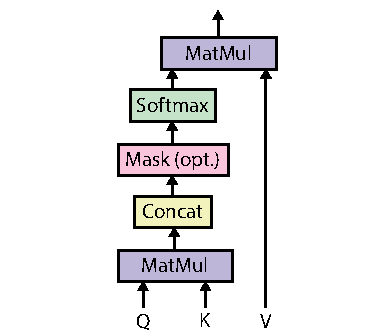
\includegraphics[width=0.8\textwidth,keepaspectratio]{figures/scaled_dot-product_attention.pdf}
        \caption{Scaled Dot-Product Attention.}
        \label{fig:scaled-dotproduct-attention}
    \end{subfigure}%
    \hfill
    \begin{subfigure}[b]{0.5\textwidth}
        \centering
        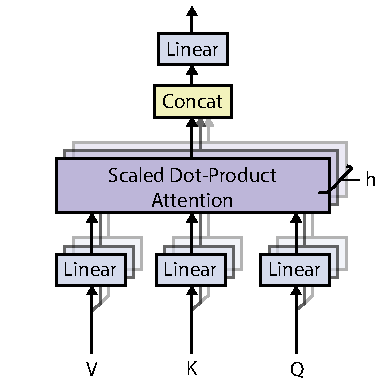
\includegraphics[width=0.8\textwidth,keepaspectratio]{figures/multi-head_attention.pdf}
        \caption{Multi-Head Attention consists of several attention layers running in parallel.}
        \label{fig:multihead-attention}
    \end{subfigure}%
    \caption{Multi-Head Attention module in Transformer architecture \textcite{vaswani2017attention}}
    \label{fig:transformer-architecture-details}
\end{figure}

\subsubsection{Scaled dot-product attention} 
\label{sec:scaled-dot-product-attention}
The self-attention layer used in each Transformer block is named "Scaled Dot-Product Attention". An overview of the attention layer is shown in \cref{fig:scaled-dotproduct-attention}. The layer learns three weight matrices, query weights \(W_Q\), key weights \(W_K\), and value weights \(W_V\). Each input word embedding is multiplied with each weight matrix, producing a query vector, key vector, and value vector. Self-attention scores are then generated by calculating the dot products of the query vector with the key vector of the respective word (query) that is calculated.

In order to stabilize the gradients during training, the attention weights are divided by the square root of the dimension of the key vectors, \(\sqrt{d_{k}}\). A softmax function is then applied, normalizing the scores to be positive and adding up to 1. Each value vector is then multiplied by the the softmax score. The resulting weighted value vectors are then summed up and serve as output from the attention layer.

In practice, the attention calculation for all tokens can be expressed as one large matrix calculation. This significantly speeds up the training process. The queries, keys, and values are packed into separate matrices. The output matrix can be described as:
\todo{T means transpose. Since this is matrix calculations, do I need to add an explanation of this?}
\begin{equation}
    \text{Attention$(Q,K,V)$} = \text{softmax}(\frac{QK^T}{\sqrt{d_{k}}})V
\end{equation}


\subsubsection{Multi-head attention}
\label{sec:multi-head-attention}
By splitting the query, key, and value parameters in N-ways (logically), each with its separate weight matrix, the performance of the Transformer is increased. This is called multi-head attention, illustrated in \cref{fig:multihead-attention}. It gives the Transformer greater power to encode multiple relationships and nuances for each word. The final attention outputs for the feed-forward network are calculated by concatenating the matrixes for each attention head.

\subsection{Training}
\label{sec:transformer-training}
A Transformer model typically undergoes something called self-supervised learning. This is an intermediary between both unsupervised- and supervised learning. This normally conforms to unsupervised pre-training the model on a large set of data. Then, the model is fine-tuned on a (usually) smaller dataset of labeled data.

In contrast to the unsupervised training, where the target sequence comprises the predicted transformer output, the supervised training is done by feeding the complete input- and target language sequence directly into the Transformer. The input sequence is fed to the encoder, while the target sequence is fed to the decoder.

\subsection{Inference}
\label{sec:transformer-inference}
For making inference, the Transformer is only fed the input sequence. The encoder is run on the input sequence, and the encoder output is fed to the decoder. Since no encoder output is available at the first timestep, the decoder is fed a special "<start>" token. The decoder output is then fed back into the decoder again. This process is repeated until the decoder output encounters a special "<stop>" token.

\todo{More concrete example to explain this. Maybe a figure?}

\section{Metrics}
\label{sec:metrics}

\subsection{Performance metric}
\label{sec:performance-metric}

\subsubsection{Accuracy}
\label{sec:accuracy}

\subsubsection{Perplexity}
\label{sec:perplexity}

\subsection{Machine translation metrics}
\label{sec:machine-translation-metrics}

\subsubsection{\textsc{Bleu}}
\label{sec:blue-score}
\acrfullr{bleu} by \textcite{papineni2002bleu} is a metric for automatically evaluating machine-translated text. \acrshort{bleu} scores are between 0 and 1. A value of 0 means there is no overlap with the reference translation, while a value of 1 means that the translation perfectly overlaps. A score of 0.6 or 0.7 is considered the best you can achieve. The method is based on n-gram matching, where n-grams in the reference translation are matched against n-grams in the translation. The matches are position-independent. The more matches, the higher the score.\\

\noindent For example, consider the following two translations:\\

\indent Candidate: \underline{on} \underline{the} \underline{mat} \underline{the} \underline{cat} sat.\\
\indent Reference: \underline{The} \underline{cat} is \underline{on} \underline{the} \underline{mat}.\\

\noindent The unigram precision \(\left(p_1\right) = 5/6\)\\

\noindent However, machine translations tend to generate an abundance of reasonable words, which could result in an inaccurately high precision. To combat this, \acrshort{bleu} uses something called modified precision. The modification consists of clipping the occurrence of an n-gram to the maximum number the n-gram occurs in the reference. These clipped precision scores \(\left(p_n\right)\) are then calculated for n-grams up to length \(N\), normally 1-grams through 4-grams. They are then combined by computing the geometric average precision. In addition, positive weights \(w_n\) are used, normally set to \(w_n = 1/N\).

\begin{equation}
    \label{eq:geometric-average-precision}
    \text{Geometric Average Precision $\left(N\right)$} = \exp \left( \sum_{n=1}^{N} w_n \log{p_n} \right)
\end{equation}

\noindent \acrshort{bleu} also introduces a brevity penalty for penalizing translations that are shorter than the reference.

\begin{equation}
    \label{eqn:brevity-penalty}
    \text{Brevity Penalty} = 
    \begin{cases}
        1 & \text{if } c > r\\
        e^{\left(1-r/c \right)} & \text{if } c \le r
    \end{cases}
\end{equation}

\noindent The final \acrshort{bleu} score is then computed as:

\begin{equation}
    \label{eqn:bleu}
    \textsc{Bleu} = \text{Brevity Penalty} \cdot \text{Geometric Average Precision Scores $\left(N\right)$}
\end{equation}

\subsection{String metric}
\label{sec:string-metric}

\subsubsection{Jaccard index}
\label{sec:jaccard-index}
TODO: Used for smart contract filtering

\section{Blockchain}
\label{sec:blockchain}
The blockchain technology was popularized by Bitcoin in 2008. Satoshi Nakamoto introduced the formal idea of blockchain as a peer-to-peer electronic cash system. It enabled users to conduct transactions without the need for a central authority. A blockchain is a growing list of records that are linked together by a cryptographic hash. Each record is called a block. The blocks contain a cryptographic hash of the previous block, a timestamp, and transactional data. By time-stamping a block, this proves that the transaction data existed when the block was published in order to get into its hash. Since all blocks contains the hash of the previous block, they end up forming a chain. In order to tamper with a block in the chain, this also requires altering all subsequent blocks. Blockchains are therefore resistant to modification. The longer the chain, the more secure it is.

Typically, blockchains are managed by a peer-to-peer network, resulting in a publicly distributed ledger. The network is composed of nodes that are connected to each other. The nodes collectively adhere to a protocol in order to communicate and validate new blocks. Blockchain records are possible to alter through a \gls{fork}. However, blockchains can be considered secure by design and present a distributed computing system with high Byzantine fault tolerance \cite{sankar2017survey}.

From Bitcoin sprang several other cryptocurrencies and blockchain platforms such as Ethereum, Litescoin, and Ripple. \cref{tab:blockchain-platforms} shows an overview of the different blockchain platforms, including the different consensus protocols, programming languages, and execution environments used. It also shows the different types of blockchains, including public, private, and hybrid.


\subsection{Ethereum blockchain}
\label{sec:ethereum}


\section{Smart Contract}
\label{sec:smart-contract}
\todo{Rewrite and adapt to vulnerabilities SoliDetector can detect.}

The term "\acrlong{sc}" was introduced with the Ethereum platform in 2014. A \acrfull{sc} is a program that is executed on a blockchain, enabling non-trusting parties to create an \textit{agreement}. \acrshortpl{sc} have enabled several interesting new concepts, such as \acrfull{nft} and entirely new business models. Since Ethereum's introduction of \acrshortpl{sc}, the platform has kept its market share as the most popular \acrshort{sc} blockchain platform. Ethereum is a open, decentralized platform that allows users to create, store, and transfer digital assets. Solidity is a programming language that is used to write smart contracts in Ethereum. Solidity is compiled down to bytecode, which is then deployed and stored on the blockchain. Ethereum also introduces the concept of gas. Ethereum describes gas as follows: \textquote{It is the fuel that allows it to operate, in the same way that a car needs gasoline to run.} \cite{ethereum2021gas}. The gas is used to pay for the cost of running the smart contract. This protects against malicious actors spamming the network \cite{ethereum2021gas}. The gas is paid in Wei, which is the smallest unit of Ethereum. Due to the immutable nature of blockchain technology, once a smart contract is deployed, it cannot be changed. This can have serious security implications, as vulnerable contracts can not be updated.

\subsection{Security Vulnerabilities}
\label{sec:smart-contract-vulnerabilities}
There are many vulnerabilities in \acrfullpl{sc} that can be exploited by malicious actors. Throughout the last years, an increase in the use of the Ethereum network has led to the development of \acrshortpl{sc} that are vulnerable to attacks. Due to the nature of blockchain technology, the attack surface of \acrshortpl{sc} is somewhat different from that of traditional computing systems. The Smart Contract Weakness Classification (SWC) Registry \footnote{\url{https://swcregistry.io}} collects information about various vulnerabilities. Following is a list of the most common vulnerabilities in \acrlongpl{sc}:

\subsubsection{Integer Overflow and Underflow}
Integer overflow and underflows happen when an arithmetic operation reaches the maximum or minimum size of a certain data type. In particular, multiplying or adding two integers may result in a value that is unexpectedly small, and subtracting from a small integer may cause a wrap to be an unexpectedly large positive value. For example, an 8-bit integer addition 255 + 2 might result in 1.

\subsubsection{Transaction-Ordering Dependence}
In blockchain systems, there is no guarantee on the execution order of transactions. A miner can influence the outcome of a transaction due to its own reordering criteria. For example, a transaction that is dependent on another transaction to be executed first may not be executed. This can be exploited by malicious actors. 

\subsubsection{Broken Access Control}
Access Control issues are common in most systems, not just smart contracts. However, due to the monetary nature and openness of most \acrshortpl{sc}, properly enforcing access controls are essential. Broken access control can, for example, occur due to wrong visibility settings, giving attackers a relatively straightforward way to access contracts' private assets. However, the bypass methods are sometimes more subtle. For example, in Solidity, reckless use of \lstinline[language=Solidity]!delegatecall! in proxy libraries, or the use of the deprecated \lstinline[language=Solidity]!tx.origin! might result in broken access control. \cref{lst:broken-access-control} shows a simple Solidity contract where anyone is able to trigger the contract's self-destruct, which makes the code vulnerable.

\begin{lstlisting}[
    caption={Access control vulnerable Solidity \acrlong{sc} code},
    label=lst:broken-access-control,
    language=Solidity]s
contract SimpleSuicide {
    function sudicideAnyone() {
        selfdestruct(msg.sender);
    }
}
\end{lstlisting}

\subsubsection{Timestamp Dependency}
If a \acrlong{sc} is dependent on the timestamp of a transaction, it is vulnerable to attacks. A miner has control over the execution environment for the executing \acrshort{sc}. If the \acrshort{sc} platform allows for \acrshortpl{sc} to use the time defined by the execution environment, this can result in a vulnerability. An example vulnerable use is a timestamp used as part of the conditions to perform a critical operation (e.g., sending ether) or as the source of entropy to generate random numbers. Hence, if the miner holds a stake in a contract, he could gain an advantage by choosing a suitable timestamp for a block he is mining. \cref{lst:timestamp-dependency} shows an example Solidity \acrshort{sc} code that contains this vulnerability. Here, the timestamp (the \lstinline[language=Solidity]!now! keyword on line 10) is used as a source of entropy to generate a random number.

\begin{lstlisting}[
    caption={Timestamp Dependency vulnerable Solidity \acrlong{sc} code},
    label=lst:timestamp-dependency,
    language=Solidity]
contract Roulette {
    uint public prevBlockTime; // One bet per block
    constructor() external payable {} // Initially fund contract
    
    // Fallback function used to make a bet
    function () external payable {
        require(msg.value == 5 ether); // Require 5 ether to play
        require(now != prevBlockTime); // Only 1 transaction per block
        prevBlockTime = now;
        if(now % 15 == 0) { // winner
            msg.sender.transfer(this.balance);
        }
    }
}
\end{lstlisting}

\subsubsection{Reentrancy}
Reentrancy is a vulnerability that occurs when a \acrshort{sc} calls external contracts. Most blockchain platforms that implement \acrshort{sc} provide a way to make external contract calls. In Ethereum, an attacker may carefully construct a \acrshort{sc} at an external address that contains malicious code in its fallback function. Then, when a contract sends funds to the address, it will invoke the malicious code. Usually, the malicious code triggers a function in the vulnerable contract, performing operations not expected by the developer. It is called "reentrancy" since the external malicious contract calls a function on the vulnerable contract and the code execution then "reenters" it. \cref{lst:reentrancy} shows a Solidity \acrshort{sc} function where a user is able to withdraw all the user's funds from a contract. If a malicious actor carefully crafts a contract that calls the withdrawal function several times before completing, the actor would successfully withdraw more funds than the current available balance. This vulnerability could be eliminated by updating the balance (line 4) before transferring the funds (line 3).

\begin{lstlisting}[
    caption={Reentrancy vulnerable Solidity \acrlong{sc} code},
    label=lst:reentrancy,
    language=Solidity]
function withdraw() external {
    uint256 amount = balances[msg.sender];
    require(msg.sender.call.value(amount)());
    balances[msg.sender] = 0;
}   
\end{lstlisting}



\section{Vulnerability detection}
\label{sec:vulnerability-detection}
\todo{Condence into one section, describing the different methods.. Add ontology based detection (for SoliDetector)}
Many tools and methods for vulnerability detection have been developed over recent years. This includes both static and dynamic vulnerability techniques, as well as tools based on \acrfull{ml}. These tools can be categorized in terms of their primary function. This includes symbolic execution, syntax analysis, abstract interpretation, data flow analysis, fuzzy testing, and machine learning. In the following sections, the identified vulnerability detection tools are summarized, compared, and analyzed in detail.

\subsection{Symbolic execution}
\label{sec:symbolic-execution}
Symbolic execution is a method for analyzing a computer program in order to determine what inputs cause each part of a program to execute. Symbolic execution requires the program to run. During the execution of the program, symbolic values are used instead of concrete values. The program execution arrives at expressions in terms of symbols for expressions and variables, as well as constraints expressed as symbols for each possible outcome of each conditional branch of the program. Finally, the possible inputs, expressed as symbols, that trigger a branch can be determined by solving the constraints.

\subsubsection{Syntax analysis}
\label{sec:syntax-analysis}
Syntax analysis is a technique for analyzing computer programs by analyzing the syntactical features of a computer program. This usually involves some kind of pattern matching where the source code is first parsed into a tree structure. This tree is then analyzed by looking for vulnerable patterns while traversing the tree.

\subsubsection{Abstract interpretation}
\label{sec:abstract-interpretation}
Abstract interpretation is a method to analyze computer programs by soundly approximating the semantics of a computer program. This results in a superset of the concrete program semantics. Normally, this is then used to automatically extract information about the possible executions of computer programs.

\subsubsection{Data flow analysis}
\label{sec:data-flow-analysis}
Data flow analysis is a method for analyzing computer programs by gathering information about the flow of data through the source code. This is done by collecting all the possible set of values calculated at different points through a computer program. This method is able to analyze large programs, compared to, for example, symbolic execution.

\subsubsection{Fuzzy testing}
\label{sec:fuzzy-testing}
Fuzzing is an automated testing technique for analyzing computer programs. The technique involves supplying invalid, unexpected, or random data inputs to a program in order to uncover bugs. The program is then monitored during execution for unexpected behavior such as crashes, errors, or failing built-in code assertions.

\chapter{Related work}
\label{chap:related-work}

This chapter presents related research in the field of source code synthesis. \cref{sec:code-synthesis} presents various techniques for code synthesis. The section begins with presenting some of the earlier techniques, followed by surveying more recent and state-of-the-art code synthesis techniques. In \cref{sec:bias-in-language-models} works related to bias in language models are presented.

%\section{Language models}
%\label{sec:language-models}
%The problem of generating code is fundamentally a language modeling problem. Language modeling is the task of predicting the next word in a text given the previous words. This section begins with presenting some of the earlier techniques, followed by surveying more recent and state-of-the-art language models.
%
%
%The first few language models came in the form of n-grams, a term first referenced by \textcite{shannon1948ngram}. An n-gram is a %contiguous sequence of n items from a given sample of text. Most early approaches employed n-grams with smoothing to handle unseen %n-grams \textcite{kneser1995improved}.
%
%\subsection{Non-context models}
%\subsection{Context aware models}
%\subsection{Word embeddings}
%Tomas Mikolov's Word2vec (google team),
%Stanford University's GloVe
%GN-GloVe (genderneutral) ->point tto thte bias problem off datasets -> link to insecure code on  github
%
%\subsection{Neural language models}
%N-grams
%
%CoVe (Contextualized Word Vectors) needs "fixed" prettrained dataset :: Learned in Translation: Contextualized Word Vectors
%
%ELMo biLM
%
%Universal Language Model Fine-tuning (ULMFiT) :: introduced the concept of fine-tuning the language model.
%
%OpenAI’s Gener- ative Pre-training Transformer (GPT)
%
%GPT-2, improved version of GPT. Works without fine-tuning. (concerns of it being used to generate unintended or malicious content - %delayed release)
%
%Bidirectional Encoder Representations from Transformers (BERT) - > bidirectttional, in comparison to GPT
%
%BERT is a bimodal Transformer with 12 layers, 768 dimentional hidden states, and 12 attention heads.
%
%-----
%GPT-3 (Codex)
%
%GPT-J (Opensoursed)
%
%
\section{Code synthesis}
\label{sec:code-synthesis}
Code synthesis is the task of generating code from a given specification. One of the earlier classical works used a probabilistic \acrfull{pcfg} \cite{allamanis2015bimodal}. \textcite{hindle2012natural} investigated whether code could be modeled by statistical language models. In particular, the authors used an n-gram model. They argue that "programs that real people actually write are mostly simple and rather repetitive, and thus they have usefully predictable statistical properties". They found that code is more predictable than natural languages. DeepCoder by \textcite{balog2017deepcoder} focused on solving programming competition-style problems. They trained a neural network for predicting properties of source code, which could be used for guiding program search.

\subsection{Code synthesis based on code semantics}
Programs can also be synthesized by leveraging the semantics of the code. \textcite{alon2018code2vec} purposes a tool named code2vec. It is a neural network model for representing snippets of code as continuously distributed vectors, or "code embeddings". The authors leverage the semantic structure of code by passing serialized \acrfullpl{ast} into a neural network. Code2seq \cite{alon2018code2seq} builds on the works of \textcite{alon2018code2vec} which focuses on natural language sequence generation from code snippets. The authors use an encoder-decoder LSTM model and rely on \acrshortpl{ast} for code snippets. The model is trained on three Java corpuses small, medium, and large, achieving a \gls{f1} score of 50.64, 53.23, and 59.19, respectively. However, the model is limited to only considering the immediately surrounding context. Pythia by \textcite{svyatkovskiy2019pyhia} is able to generate ranked lists of method and API recommendations to be used by software developers at edit time. The code completion system is based on \acrshortpl{ast} and uses Word2vec for producing code embeddings of Python code. These code embeddings are then used to train a \gls{lstm} model. The model is evaluated on a dataset of 15.8 million method calls extracted from real-world source code, achieving an accuracy of 92\%.

\subsection{Code synthesis based on transformers}
\label{sec:transformers-for-code-synthesis}
Inspired by the success of large natural language models such as \acrfullr{elmo} \cite{peters2018deep}, \acrfullr{gpt} \cite{radford2018improving}, \acrfullr{bert} \cite{devlin2018bert}, XLNet \cite{yang2019xlnet}, and RoBERTa \cite{liu2019roberta}, large-scale Transformer models have been applied in the domains of code synthesis. \textcite{feng2020codebert} proposes a new approach to code synthesis by training the BERT transformer model on Python \gls{docstring} paired with functions. The resulting 125M parameter transformer model, named CodeBERT \cite{feng2020codebert}, achieves strong results on code-search and code-to-text generation. The authors also observe that models that leverage code semantics (\acrshortpl{ast}) can produce slightly better results. PyMT5 \textcite{colin2020pymt5} is based on the T5 model. The model can predict whole methods from natural language documentation strings (docstrings) and summarize code into docstrings of any common style. For method generation, PyMT5 achieves a \gls{bleu} score of 0.0859 and a F-score of 24.8 on the CodeSearchNet \cite{codesearchnet} test set. GPT-C by \textcite{svyatkovskiy2020intellicode} is a model based on GPT-2. The 366M parameter-sized model is trained on a code corpus consisting of 1.2 billion lines of source code in Python, C\#, JavaScript and TypeScript programming languages. The Python-only model reportedly achieves a ROUGE-L precision of 0.80 and recall of 0.86.

The model complexity of transformers has recently sky-rocketed, with model sizes growing to several tens of billions of parameters. GPT-J is a 6 billion parameter model trained on The Pile, which is an 825GB dataset. The pre-trained version of GPT-J is also publicly available. Codex by \textcite{chen2021codex} is a 12 billion parameter model based on GPT. It was trained on 54 million GitHub repositories, and a production version of Codex powers GitHub Copilot \cite{copilot}. The model solves 28.8\% of the problems in the HumanEval dataset \cite{chen2021codex}, while GPT-3 solves 0\% and GPT-J solves 11.4\%. Google DeepMind's AlphaCode \cite{alphacode} is 41.4 billion parameters and is the first AI to reach a competitive level in programming competitions. AlphaCode was tested against challenges curated by Codeforces \cite{codeforces}, a competitive coding platform. It achieved an average ranking of 54.3\% across 10 contests. The authors found that repeated sampling on the same problem significantly increased the probability of a correct solution.


\newcommand*\emptycirc[1][1ex]{\tikz\draw (0,0) circle (#1);} 
\newcommand*\halfcirc[1][1ex]{%
  \begin{tikzpicture}
  \draw[fill] (0,0)-- (90:#1) arc (90:270:#1) -- cycle ;
  \draw (0,0) circle (#1);
  \end{tikzpicture}}
\newcommand*\fullcirc[1][1ex]{\tikz\fill (0,0) circle (#1);} 


%\begin{sidewaystable}
\begin{ThreePartTable}
    \newcolumntype{Y}{>{\centering\arraybackslash}X}
    \newcolumntype{R}{>{\raggedright\arraybackslash}X}
    \def\arraystretch{1.5}
    \setlength\tabcolsep{6pt} % <--- important, (default 6pt)
    \setlength{\LTleft}{-20cm plus -1fill}
    \setlength{\LTright}{\LTleft}
    \footnotesize
    \begin{center}
    \keepXColumns
    \begin{tabularx}{1\textwidth}{clRRRRR}
            \caption{Existing language models.}\label{tab:code-synthesis-models}\\
            \toprule
            \textbf{Refs.} & \textbf{Year} & \textbf{Model} & \textbf{Metrics} & \textbf{Languages} &  \textbf{Input} & \textbf{Output}\\
            \hline
            \endfirsthead
            \caption{(\textit{Continued}) Existing static smart contract vulnerability detection tools.}\\
            \toprule
            \textbf{Refs.} & \textbf{Year} & \textbf{Model} & \textbf{Metrics} & \textbf{Languages} &  \textbf{Input} & \textbf{Output}\\
            \hline
        \endhead
            \midrule
            \multicolumn{7}{r}{\small(\textit{Continued on next page})}\\
        \endfoot
        \endlastfoot
        
        \cite{feng2020codebert} & \citeyear{feng2020codebert} & CodeBERT & \acrshort{bleu} & Python  & Code & Docstring\\
        \cite{colin2020pymt5} & \citeyear{colin2020pymt5} & PyMT5 & \acrshort{bleu} & Python & Docstring & Code\\
        \cite{svyatkovskiy2020intellicode} & \citeyear{svyatkovskiy2020intellicode} & GPT-C & ROUGE-L & Python, C\#, JavaScript, TypeScript &  & \\
        \cite{chen2021codex} & \citeyear{chen2021codex} & Codex & Functional correctness & Python & Docstring & Code\\
        \cite{alphacode} & \citeyear{alphacode} & AlphaCode & Functional correctness & Python, C++, Java & Problem  description & Code\\
        \bottomrule
    \end{tabularx}
    \end{center}

\end{ThreePartTable}
%\end{sidewaystable}

As can be seen from \cref{tab:code-synthesis-models}, most of the models are concerned with Python code. However, none have attempted to generate \acrfullpl{sc} code. \acrshort{sc} code is quite different from most of the other popular languages such as Python, JavaScript, and Java. Investigating how transformer models perform on \acrshort{sc} code would give valuable insight into the future of code synthesis. Further, all of the works listed in \cref{tab:code-synthesis-models} that are concerned with text-to-code generation, only consider using comments in isolation. There is therefore a need for an investigation of a code generation approach that uses both comments and code for generating functions.

\section{Bias in language models}
\label{sec:bias-in-language-models}
One of the main problems with language models is that they often contain bias \cite{li2021detecting}. This can be everything from producing gender-specific jobs to favoring a certain race. There have been several works related to mitigating this in language models. However, with varying success. \textcite{Silva2021TowardsAC} tried to mitigate societal bias in text generation using a loss regularizer to “de-bias” a RoBERTa model. However, their approach was not successful and conclude there is a need for more robust bias testing in transformers. Several works are devoted to using adversarial methods to reduce bias. \textcite{laftr2018} propose LAFTER, an adversarial method to modify the training objective based on a desired fairness measure. \textcite{zhang2018mitigating} also tries to reduce bias using adversarial training. However, \cite{zhang2018mitigating} states that the adversarial training method is hard to get right and is often touchy. \textcite{mitigating2021} investigates bias in visual transformer models, as they find existing approaches such as LAFTR unable to maintain high performance. They propose TADeT, a targeted alignment strategy for debasing transformers that aims to discover and remove bias primarily from query matrix features. 

In the area of code synthesis, vulnerabilities can be considered a form of bias in language models. However, there seems to be very little research on the security of synthesized code using transformers. \cite{chen2021codex} provide a brief discussion of insecure code generated by Codex. However, this investigation was limited to the exploration of the generation of cryptographic functions. \textcite{pearch2021asleep} acknowledge this gap in research and conduct a vulnerability analysis of GitHub Copilot (based on Codex). They construct a manual dataset of incomplete python and C code that \textit{may} produce a vulnerability. From their analysis of 1689 synthesized Python and C programs, they conclude with approximately 40\% are vulnerable. This shows there is a dire need for reducing the number of vulnerabilities generated with language models.


% vvvvvvvv VIKTIG vvvvvvvvvv

%autoregressive generation tasks
%see https://arxiv.org/pdf/2005.08025.pdf for structuring thesisl....!!!!

%see docstring analysis 2.3 of https://arxiv.org/pdf/2010.03150.pdf for clustering comments....
%^^^^^^^^ VIKTIG ^^^^^^^^


%\todo{Try to find papers that reviewe style of comments}
%Several papers on generating code comments from source code are available. The following is a list of the most popular papers.

%However, to the best of my knowledge, there is no paper investigating how to best write comments for auto-generating code. There are however, 




\chapter{Method}
\label{chap:method}
This chapter presents the research method used in this thesis. Firstly, the research motivation is presented, followed by the research questions defined for this thesis. Finally, the research method and design is explained.

\section{Research Motivation}

Existing solutions are slow.
A total of X new contrats are deployed  each day on the Ethereum network. Witth tthe speedup of the upgraded ethereum network,  this is likely to result in an utterly spike  in deployed contracts. Existing solutions are scarse. Further, the few ones available are based on symbolic analysis.  Tthis is a very slow approach. It is therefore not possible to process all new contractts due to time resttrictions. An natural approach for combatting this is by leveraging deep learning techniques.





\section{Research Questions}
\label{sec:research-questions}
The research questions addressed in this thesis are:
\begin{enumerate}[label=RQ\arabic*., leftmargin=1.5cm]
    \item Officia magna irure ut occaecat cupidatat non sunt sunt.
\end{enumerate}

\section{Research Method and Design}
\label{sec:research-method-and-design}

\begin{figure}[htp]
    \centering
    \includegraphics[width=\textwidth]{example-image-a}
    \caption{Flowchart of.....}
    \label{fig:flowchart}
\end{figure}

\section{Tools and Libraries}
\label{sec:tools-and-libraries}

\section{Hardware resources}
\label{sec:hardware-resources}

\subsection{IDUN High Performance Computing Platform}
\label{sec:idun-high-performance-computing-platform}
\chapter{Data}
\label{chap:datasets}
This chapter introduces the necessary background information for this study. First, a brief introduction to blockchain technology is provided in \cref{sec:blockchain} and then the concept of \acrfullpl{sc} is introduced in \cref{sec:smart-contract}. Finally, in \cref{sec:smart-contract-vulnerabilities}, the most popular \acrshort{sc} vulnerabilities are described.

\section{Smart contract downloader}
\label{sec:smart-contract-downloader}
\url{https://github.com/andstor/smart-contract-downloader}


The largest provider of verified \acrshortpl{sc} is Etherscan. This website provides a list of all verified \acrshortpl{sc} on the blockchain. More on their service...... Etherscan provides a API for downloading verified Smart Contracts. The API is available at \url{https://api.etherscan.io/api}.

In order to download the \acrshortpl{sc} from Etherscan, a tool we need to provide the \acrshortpl{sc} address. The address is the first part of the \acrshortpl{sc} code. The address is the first part of the \acrshortpl{sc} code.

The following code snippet is a Google BigQuery query. It will select all \acrshortpl{sc} addresses on the Ethereum blockchain that has at least one transaction. This query was run on the 1st of April 2022, and the result was downloaded as a CSV file, and is available at \url{https://huggingface.co/datasets/andstor/smart_contracts/blob/main/contract_addresses.csv}. The CSV file is then used to download the \acrshortpl{sc} from Etherscan.

\begin{lstlisting}[
    caption={Google BigQuery query for selecting all \acrlong{sc} addresses on Ethereum that has at least one transaction.},
    label=lst:reentrancy,
    language=SQL]
SELECT contracts.address, COUNT(1) AS tx_count
FROM `bigquery-public-data.crypto_ethereum.contracts` AS contracts
JOIN `bigquery-public-data.crypto_ethereum.transactions` AS transactions 
      ON (transactions.to_address = contracts.address)
GROUP BY contracts.address
ORDER BY tx_count DESC
}
\end{lstlisting}

\section{Datasets}
Describe the  PILE...  It consists  of among others a lot of data from GitHub. HHowever, only x\% of the data is smart contracts (Solidity). Hence there is a need  for a dataset made up of smart contracts. --> existing datasets....

\subsection{Verified Smart Contracts}
\label{sec:verified-smart-contracts}
\url{https://github.com/andstor/verified-smart-contracts}
\url{https://huggingface.co/datasets/andstor/smart_contracts}


Filtering is done by applying a token-based similarity algorithm, named Jacard Index. Thte algorithm  is computationally efficient and can be used to filter out \acrshortpl{sc} that are not similar to the query. The Jacard Index is a measure of the similarity between two sets. The Jacard Index is defined as the ratio of the size of the intersection to the size of the union of the two sets.....

\makeatletter
\newcommand\thefontsize[1]{{#1 The current font size is: \f@size pt\par}}
\makeatother

\thefontsize\tiny
\thefontsize\footnotesize
\thefontsize\small
\thefontsize\normalsize
\thefontsize\large

\extractcolorspecs{red!50}{\model}{\mycolor}
\convertcolorspec{\model}{\mycolor}{rgb}\tmp\tmp

\extractcolorspecs{green!30!white}{\model}{\mycolor}
\convertcolorspec{\model}{\mycolor}{rgb}\tmp\tmp

\extractcolorspecs{blue!30!white}{\model}{\mycolor}
\convertcolorspec{\model}{\mycolor}{rgb}\tmp\tmp

\printinunitsof{in}\prntlen{\textwidth}

Subsets:
\subsubsection{Raw}
\label{sec:verified-smart-contracts-raw}


\begin{figure}[ht]
    \centering
    %% Creator: Matplotlib, PGF backend
%%
%% To include the figure in your LaTeX document, write
%%   \input{<filename>.pgf}
%%
%% Make sure the required packages are loaded in your preamble
%%   \usepackage{pgf}
%%
%% and, on pdftex
%%   \usepackage[utf8]{inputenc}\DeclareUnicodeCharacter{2212}{-}
%%
%% or, on luatex and xetex
%%   \usepackage{unicode-math}
%%
%% Figures using additional raster images can only be included by \input if
%% they are in the same directory as the main LaTeX file. For loading figures
%% from other directories you can use the `import` package
%%   \usepackage{import}
%%
%% and then include the figures with
%%   \import{<path to file>}{<filename>.pgf}
%%
%% Matplotlib used the following preamble
%%
\begingroup%
\makeatletter%
\begin{pgfpicture}%
\pgfpathrectangle{\pgfpointorigin}{\pgfqpoint{3.449272in}{3.773420in}}%
\pgfusepath{use as bounding box, clip}%
\begin{pgfscope}%
\pgfsetbuttcap%
\pgfsetmiterjoin%
\definecolor{currentfill}{rgb}{1.000000,1.000000,1.000000}%
\pgfsetfillcolor{currentfill}%
\pgfsetlinewidth{0.000000pt}%
\definecolor{currentstroke}{rgb}{1.000000,1.000000,1.000000}%
\pgfsetstrokecolor{currentstroke}%
\pgfsetdash{}{0pt}%
\pgfpathmoveto{\pgfqpoint{0.000000in}{-0.000000in}}%
\pgfpathlineto{\pgfqpoint{3.449272in}{-0.000000in}}%
\pgfpathlineto{\pgfqpoint{3.449272in}{3.773420in}}%
\pgfpathlineto{\pgfqpoint{0.000000in}{3.773420in}}%
\pgfpathclose%
\pgfusepath{fill}%
\end{pgfscope}%
\begin{pgfscope}%
\pgfsetbuttcap%
\pgfsetmiterjoin%
\definecolor{currentfill}{rgb}{0.475341,0.000000,0.943137}%
\pgfsetfillcolor{currentfill}%
\pgfsetfillopacity{0.700000}%
\pgfsetlinewidth{0.000000pt}%
\definecolor{currentstroke}{rgb}{0.000000,0.000000,0.000000}%
\pgfsetstrokecolor{currentstroke}%
\pgfsetstrokeopacity{0.700000}%
\pgfsetdash{}{0pt}%
\pgfpathmoveto{\pgfqpoint{2.651052in}{2.128968in}}%
\pgfpathcurveto{\pgfqpoint{2.651052in}{2.133588in}}{\pgfqpoint{2.651020in}{2.138209in}}{\pgfqpoint{2.650958in}{2.142829in}}%
\pgfpathcurveto{\pgfqpoint{2.650895in}{2.147449in}}{\pgfqpoint{2.650801in}{2.152068in}}{\pgfqpoint{2.650675in}{2.156687in}}%
\pgfpathlineto{\pgfqpoint{2.140693in}{2.142827in}}%
\pgfpathcurveto{\pgfqpoint{2.140756in}{2.140518in}}{\pgfqpoint{2.140803in}{2.138208in}}{\pgfqpoint{2.140834in}{2.135898in}}%
\pgfpathcurveto{\pgfqpoint{2.140866in}{2.133588in}}{\pgfqpoint{2.140881in}{2.131278in}}{\pgfqpoint{2.140881in}{2.128968in}}%
\pgfpathlineto{\pgfqpoint{2.651052in}{2.128968in}}%
\pgfpathclose%
\pgfusepath{fill}%
\end{pgfscope}%
\begin{pgfscope}%
\pgfsetbuttcap%
\pgfsetmiterjoin%
\definecolor{currentfill}{rgb}{0.882745,0.000000,0.111414}%
\pgfsetfillcolor{currentfill}%
\pgfsetfillopacity{0.700000}%
\pgfsetlinewidth{0.000000pt}%
\definecolor{currentstroke}{rgb}{0.000000,0.000000,0.000000}%
\pgfsetstrokecolor{currentstroke}%
\pgfsetstrokeopacity{0.700000}%
\pgfsetdash{}{0pt}%
\pgfpathmoveto{\pgfqpoint{2.650675in}{2.156687in}}%
\pgfpathcurveto{\pgfqpoint{2.643613in}{2.416544in}}{\pgfqpoint{2.537505in}{2.664127in}}{\pgfqpoint{2.354202in}{2.848452in}}%
\pgfpathcurveto{\pgfqpoint{2.170898in}{3.032777in}}{\pgfqpoint{1.923908in}{3.140258in}}{\pgfqpoint{1.664093in}{3.148763in}}%
\pgfpathcurveto{\pgfqpoint{1.404279in}{3.157268in}}{\pgfqpoint{1.150788in}{3.066169in}}{\pgfqpoint{0.955822in}{2.894227in}}%
\pgfpathcurveto{\pgfqpoint{0.760856in}{2.722285in}}{\pgfqpoint{0.638784in}{2.482171in}}{\pgfqpoint{0.614743in}{2.223332in}}%
\pgfpathlineto{\pgfqpoint{1.122727in}{2.176150in}}%
\pgfpathcurveto{\pgfqpoint{1.134747in}{2.305570in}}{\pgfqpoint{1.195784in}{2.425626in}}{\pgfqpoint{1.293267in}{2.511598in}}%
\pgfpathcurveto{\pgfqpoint{1.390750in}{2.597569in}}{\pgfqpoint{1.517495in}{2.643118in}}{\pgfqpoint{1.647402in}{2.638866in}}%
\pgfpathcurveto{\pgfqpoint{1.777309in}{2.634613in}}{\pgfqpoint{1.900804in}{2.580872in}}{\pgfqpoint{1.992456in}{2.488710in}}%
\pgfpathcurveto{\pgfqpoint{2.084108in}{2.396548in}}{\pgfqpoint{2.137162in}{2.272756in}}{\pgfqpoint{2.140693in}{2.142827in}}%
\pgfpathlineto{\pgfqpoint{2.650675in}{2.156687in}}%
\pgfpathclose%
\pgfusepath{fill}%
\end{pgfscope}%
\begin{pgfscope}%
\pgfsetbuttcap%
\pgfsetmiterjoin%
\definecolor{currentfill}{rgb}{0.000000,0.786667,0.312353}%
\pgfsetfillcolor{currentfill}%
\pgfsetfillopacity{0.700000}%
\pgfsetlinewidth{0.000000pt}%
\definecolor{currentstroke}{rgb}{0.000000,0.000000,0.000000}%
\pgfsetstrokecolor{currentstroke}%
\pgfsetstrokeopacity{0.700000}%
\pgfsetdash{}{0pt}%
\pgfpathmoveto{\pgfqpoint{0.614743in}{2.223332in}}%
\pgfpathcurveto{\pgfqpoint{0.611982in}{2.193606in}}{\pgfqpoint{0.610527in}{2.163774in}}{\pgfqpoint{0.610382in}{2.133921in}}%
\pgfpathcurveto{\pgfqpoint{0.610237in}{2.104068in}}{\pgfqpoint{0.611402in}{2.074223in}}{\pgfqpoint{0.613874in}{2.044472in}}%
\pgfpathlineto{\pgfqpoint{1.122293in}{2.086720in}}%
\pgfpathcurveto{\pgfqpoint{1.121057in}{2.101596in}}{\pgfqpoint{1.120474in}{2.116518in}}{\pgfqpoint{1.120546in}{2.131445in}}%
\pgfpathcurveto{\pgfqpoint{1.120619in}{2.146371in}}{\pgfqpoint{1.121346in}{2.161287in}}{\pgfqpoint{1.122727in}{2.176150in}}%
\pgfpathlineto{\pgfqpoint{0.614743in}{2.223332in}}%
\pgfpathclose%
\pgfusepath{fill}%
\end{pgfscope}%
\begin{pgfscope}%
\pgfsetbuttcap%
\pgfsetmiterjoin%
\definecolor{currentfill}{rgb}{0.930307,0.285685,0.029301}%
\pgfsetfillcolor{currentfill}%
\pgfsetfillopacity{0.700000}%
\pgfsetlinewidth{0.000000pt}%
\definecolor{currentstroke}{rgb}{0.000000,0.000000,0.000000}%
\pgfsetstrokecolor{currentstroke}%
\pgfsetstrokeopacity{0.700000}%
\pgfsetdash{}{0pt}%
\pgfpathmoveto{\pgfqpoint{0.613874in}{2.044472in}}%
\pgfpathcurveto{\pgfqpoint{0.633145in}{1.812567in}}{\pgfqpoint{0.731182in}{1.594089in}}{\pgfqpoint{0.891613in}{1.425527in}}%
\pgfpathcurveto{\pgfqpoint{1.052044in}{1.256964in}}{\pgfqpoint{1.265411in}{1.148252in}}{\pgfqpoint{1.496081in}{1.117548in}}%
\pgfpathlineto{\pgfqpoint{1.563396in}{1.623258in}}%
\pgfpathcurveto{\pgfqpoint{1.448061in}{1.638610in}}{\pgfqpoint{1.341377in}{1.692966in}}{\pgfqpoint{1.261162in}{1.777247in}}%
\pgfpathcurveto{\pgfqpoint{1.180946in}{1.861529in}}{\pgfqpoint{1.131928in}{1.970768in}}{\pgfqpoint{1.122293in}{2.086720in}}%
\pgfpathlineto{\pgfqpoint{0.613874in}{2.044472in}}%
\pgfpathclose%
\pgfusepath{fill}%
\end{pgfscope}%
\begin{pgfscope}%
\pgfsetbuttcap%
\pgfsetmiterjoin%
\definecolor{currentfill}{rgb}{0.063700,0.382199,0.851986}%
\pgfsetfillcolor{currentfill}%
\pgfsetfillopacity{0.700000}%
\pgfsetlinewidth{0.000000pt}%
\definecolor{currentstroke}{rgb}{0.000000,0.000000,0.000000}%
\pgfsetstrokecolor{currentstroke}%
\pgfsetstrokeopacity{0.700000}%
\pgfsetdash{}{0pt}%
\pgfpathmoveto{\pgfqpoint{1.496081in}{1.117548in}}%
\pgfpathcurveto{\pgfqpoint{1.640169in}{1.098369in}}{\pgfqpoint{1.786706in}{1.110199in}}{\pgfqpoint{1.925851in}{1.152245in}}%
\pgfpathcurveto{\pgfqpoint{2.064996in}{1.194291in}}{\pgfqpoint{2.193564in}{1.265590in}}{\pgfqpoint{2.302919in}{1.361354in}}%
\pgfpathcurveto{\pgfqpoint{2.412274in}{1.457117in}}{\pgfqpoint{2.499914in}{1.575153in}}{\pgfqpoint{2.559952in}{1.707534in}}%
\pgfpathcurveto{\pgfqpoint{2.619990in}{1.839914in}}{\pgfqpoint{2.651052in}{1.983609in}}{\pgfqpoint{2.651052in}{2.128968in}}%
\pgfpathlineto{\pgfqpoint{2.140881in}{2.128968in}}%
\pgfpathcurveto{\pgfqpoint{2.140881in}{2.056289in}}{\pgfqpoint{2.125350in}{1.984441in}}{\pgfqpoint{2.095331in}{1.918251in}}%
\pgfpathcurveto{\pgfqpoint{2.065312in}{1.852060in}}{\pgfqpoint{2.021493in}{1.793043in}}{\pgfqpoint{1.966815in}{1.745161in}}%
\pgfpathcurveto{\pgfqpoint{1.912137in}{1.697279in}}{\pgfqpoint{1.847854in}{1.661630in}}{\pgfqpoint{1.778281in}{1.640607in}}%
\pgfpathcurveto{\pgfqpoint{1.708709in}{1.619584in}}{\pgfqpoint{1.635440in}{1.613668in}}{\pgfqpoint{1.563396in}{1.623258in}}%
\pgfpathlineto{\pgfqpoint{1.496081in}{1.117548in}}%
\pgfpathclose%
\pgfusepath{fill}%
\end{pgfscope}%
\begin{pgfscope}%
\pgfsetbuttcap%
\pgfsetmiterjoin%
\definecolor{currentfill}{rgb}{0.475341,0.000000,0.943137}%
\pgfsetfillcolor{currentfill}%
\pgfsetfillopacity{0.700000}%
\pgfsetlinewidth{0.000000pt}%
\definecolor{currentstroke}{rgb}{0.000000,0.000000,0.000000}%
\pgfsetstrokecolor{currentstroke}%
\pgfsetstrokeopacity{0.700000}%
\pgfsetdash{}{0pt}%
\pgfpathmoveto{\pgfqpoint{3.161222in}{2.128968in}}%
\pgfpathcurveto{\pgfqpoint{3.161222in}{2.135899in}}{\pgfqpoint{3.161175in}{2.142829in}}{\pgfqpoint{3.161081in}{2.149759in}}%
\pgfpathcurveto{\pgfqpoint{3.160987in}{2.156689in}}{\pgfqpoint{3.160846in}{2.163618in}}{\pgfqpoint{3.160658in}{2.170546in}}%
\pgfpathlineto{\pgfqpoint{2.650675in}{2.156687in}}%
\pgfpathcurveto{\pgfqpoint{2.650801in}{2.152068in}}{\pgfqpoint{2.650895in}{2.147449in}}{\pgfqpoint{2.650958in}{2.142829in}}%
\pgfpathcurveto{\pgfqpoint{2.651020in}{2.138209in}}{\pgfqpoint{2.651052in}{2.133588in}}{\pgfqpoint{2.651052in}{2.128968in}}%
\pgfpathlineto{\pgfqpoint{3.161222in}{2.128968in}}%
\pgfpathclose%
\pgfusepath{fill}%
\end{pgfscope}%
\begin{pgfscope}%
\pgfsetbuttcap%
\pgfsetmiterjoin%
\definecolor{currentfill}{rgb}{0.882745,0.000000,0.111414}%
\pgfsetfillcolor{currentfill}%
\pgfsetfillopacity{0.700000}%
\pgfsetlinewidth{0.000000pt}%
\definecolor{currentstroke}{rgb}{0.000000,0.000000,0.000000}%
\pgfsetstrokecolor{currentstroke}%
\pgfsetstrokeopacity{0.700000}%
\pgfsetdash{}{0pt}%
\pgfpathmoveto{\pgfqpoint{3.160658in}{2.170546in}}%
\pgfpathcurveto{\pgfqpoint{3.159046in}{2.229862in}}{\pgfqpoint{3.153985in}{2.289035in}}{\pgfqpoint{3.145503in}{2.347763in}}%
\pgfpathcurveto{\pgfqpoint{3.137020in}{2.406492in}}{\pgfqpoint{3.125129in}{2.464678in}}{\pgfqpoint{3.109890in}{2.522026in}}%
\pgfpathlineto{\pgfqpoint{2.616830in}{2.391007in}}%
\pgfpathcurveto{\pgfqpoint{2.626990in}{2.352775in}}{\pgfqpoint{2.634917in}{2.313984in}}{\pgfqpoint{2.640572in}{2.274832in}}%
\pgfpathcurveto{\pgfqpoint{2.646227in}{2.235679in}}{\pgfqpoint{2.649601in}{2.196231in}}{\pgfqpoint{2.650675in}{2.156687in}}%
\pgfpathlineto{\pgfqpoint{3.160658in}{2.170546in}}%
\pgfpathclose%
\pgfusepath{fill}%
\end{pgfscope}%
\begin{pgfscope}%
\pgfsetbuttcap%
\pgfsetmiterjoin%
\definecolor{currentfill}{rgb}{0.917292,0.307374,0.323876}%
\pgfsetfillcolor{currentfill}%
\pgfsetfillopacity{0.700000}%
\pgfsetlinewidth{0.000000pt}%
\definecolor{currentstroke}{rgb}{0.000000,0.000000,0.000000}%
\pgfsetstrokecolor{currentstroke}%
\pgfsetstrokeopacity{0.700000}%
\pgfsetdash{}{0pt}%
\pgfpathmoveto{\pgfqpoint{3.109890in}{2.522026in}}%
\pgfpathcurveto{\pgfqpoint{3.091225in}{2.592268in}}{\pgfqpoint{3.067580in}{2.661092in}}{\pgfqpoint{3.039134in}{2.727974in}}%
\pgfpathcurveto{\pgfqpoint{3.010689in}{2.794857in}}{\pgfqpoint{2.977516in}{2.859628in}}{\pgfqpoint{2.939867in}{2.921797in}}%
\pgfpathlineto{\pgfqpoint{2.503481in}{2.657520in}}%
\pgfpathcurveto{\pgfqpoint{2.528581in}{2.616075in}}{\pgfqpoint{2.550696in}{2.572894in}}{\pgfqpoint{2.569660in}{2.528306in}}%
\pgfpathcurveto{\pgfqpoint{2.588623in}{2.483717in}}{\pgfqpoint{2.604387in}{2.437835in}}{\pgfqpoint{2.616830in}{2.391007in}}%
\pgfpathlineto{\pgfqpoint{3.109890in}{2.522026in}}%
\pgfpathclose%
\pgfusepath{fill}%
\end{pgfscope}%
\begin{pgfscope}%
\pgfsetbuttcap%
\pgfsetmiterjoin%
\definecolor{currentfill}{rgb}{0.989063,0.592703,0.504860}%
\pgfsetfillcolor{currentfill}%
\pgfsetfillopacity{0.700000}%
\pgfsetlinewidth{0.000000pt}%
\definecolor{currentstroke}{rgb}{0.000000,0.000000,0.000000}%
\pgfsetstrokecolor{currentstroke}%
\pgfsetstrokeopacity{0.700000}%
\pgfsetdash{}{0pt}%
\pgfpathmoveto{\pgfqpoint{2.939867in}{2.921797in}}%
\pgfpathcurveto{\pgfqpoint{2.822564in}{3.115492in}}{\pgfqpoint{2.663723in}{3.280762in}}{\pgfqpoint{2.474832in}{3.405653in}}%
\pgfpathcurveto{\pgfqpoint{2.285940in}{3.530545in}}{\pgfqpoint{2.071665in}{3.611973in}}{\pgfqpoint{1.847502in}{3.644048in}}%
\pgfpathlineto{\pgfqpoint{1.775238in}{3.139021in}}%
\pgfpathcurveto{\pgfqpoint{1.924680in}{3.117638in}}{\pgfqpoint{2.067531in}{3.063353in}}{\pgfqpoint{2.193458in}{2.980092in}}%
\pgfpathcurveto{\pgfqpoint{2.319386in}{2.896831in}}{\pgfqpoint{2.425280in}{2.786651in}}{\pgfqpoint{2.503481in}{2.657520in}}%
\pgfpathlineto{\pgfqpoint{2.939867in}{2.921797in}}%
\pgfpathclose%
\pgfusepath{fill}%
\end{pgfscope}%
\begin{pgfscope}%
\pgfsetbuttcap%
\pgfsetmiterjoin%
\definecolor{currentfill}{rgb}{0.991894,0.815723,0.745126}%
\pgfsetfillcolor{currentfill}%
\pgfsetfillopacity{0.700000}%
\pgfsetlinewidth{0.000000pt}%
\definecolor{currentstroke}{rgb}{0.000000,0.000000,0.000000}%
\pgfsetstrokecolor{currentstroke}%
\pgfsetstrokeopacity{0.700000}%
\pgfsetdash{}{0pt}%
\pgfpathmoveto{\pgfqpoint{1.847502in}{3.644048in}}%
\pgfpathcurveto{\pgfqpoint{1.642231in}{3.673420in}}{\pgfqpoint{1.433115in}{3.660771in}}{\pgfqpoint{1.232881in}{3.606871in}}%
\pgfpathcurveto{\pgfqpoint{1.032647in}{3.552971in}}{\pgfqpoint{0.845439in}{3.458936in}}{\pgfqpoint{0.682651in}{3.330487in}}%
\pgfpathcurveto{\pgfqpoint{0.519863in}{3.202039in}}{\pgfqpoint{0.384864in}{3.041837in}}{\pgfqpoint{0.285870in}{2.859631in}}%
\pgfpathcurveto{\pgfqpoint{0.186876in}{2.677425in}}{\pgfqpoint{0.125936in}{2.476986in}}{\pgfqpoint{0.106759in}{2.270513in}}%
\pgfpathlineto{\pgfqpoint{0.614743in}{2.223332in}}%
\pgfpathcurveto{\pgfqpoint{0.627528in}{2.360980in}}{\pgfqpoint{0.668154in}{2.494606in}}{\pgfqpoint{0.734150in}{2.616077in}}%
\pgfpathcurveto{\pgfqpoint{0.800146in}{2.737548in}}{\pgfqpoint{0.890146in}{2.844349in}}{\pgfqpoint{0.998671in}{2.929981in}}%
\pgfpathcurveto{\pgfqpoint{1.107197in}{3.015613in}}{\pgfqpoint{1.232001in}{3.078303in}}{\pgfqpoint{1.365491in}{3.114237in}}%
\pgfpathcurveto{\pgfqpoint{1.498980in}{3.150170in}}{\pgfqpoint{1.638391in}{3.158603in}}{\pgfqpoint{1.775238in}{3.139021in}}%
\pgfpathlineto{\pgfqpoint{1.847502in}{3.644048in}}%
\pgfpathclose%
\pgfusepath{fill}%
\end{pgfscope}%
\begin{pgfscope}%
\pgfsetbuttcap%
\pgfsetmiterjoin%
\definecolor{currentfill}{rgb}{0.000000,0.786667,0.312353}%
\pgfsetfillcolor{currentfill}%
\pgfsetfillopacity{0.700000}%
\pgfsetlinewidth{0.000000pt}%
\definecolor{currentstroke}{rgb}{0.000000,0.000000,0.000000}%
\pgfsetstrokecolor{currentstroke}%
\pgfsetstrokeopacity{0.700000}%
\pgfsetdash{}{0pt}%
\pgfpathmoveto{\pgfqpoint{0.106759in}{2.270513in}}%
\pgfpathcurveto{\pgfqpoint{0.102617in}{2.225925in}}{\pgfqpoint{0.100435in}{2.181177in}}{\pgfqpoint{0.100217in}{2.136397in}}%
\pgfpathcurveto{\pgfqpoint{0.100000in}{2.091618in}}{\pgfqpoint{0.101748in}{2.046851in}}{\pgfqpoint{0.105456in}{2.002225in}}%
\pgfpathlineto{\pgfqpoint{0.613874in}{2.044472in}}%
\pgfpathcurveto{\pgfqpoint{0.611402in}{2.074223in}}{\pgfqpoint{0.610237in}{2.104068in}}{\pgfqpoint{0.610382in}{2.133921in}}%
\pgfpathcurveto{\pgfqpoint{0.610527in}{2.163774in}}{\pgfqpoint{0.611982in}{2.193606in}}{\pgfqpoint{0.614743in}{2.223332in}}%
\pgfpathlineto{\pgfqpoint{0.106759in}{2.270513in}}%
\pgfpathclose%
\pgfusepath{fill}%
\end{pgfscope}%
\begin{pgfscope}%
\pgfsetbuttcap%
\pgfsetmiterjoin%
\definecolor{currentfill}{rgb}{0.930307,0.285685,0.029301}%
\pgfsetfillcolor{currentfill}%
\pgfsetfillopacity{0.700000}%
\pgfsetlinewidth{0.000000pt}%
\definecolor{currentstroke}{rgb}{0.000000,0.000000,0.000000}%
\pgfsetstrokecolor{currentstroke}%
\pgfsetstrokeopacity{0.700000}%
\pgfsetdash{}{0pt}%
\pgfpathmoveto{\pgfqpoint{0.105456in}{2.002225in}}%
\pgfpathcurveto{\pgfqpoint{0.124422in}{1.773989in}}{\pgfqpoint{0.194377in}{1.552894in}}{\pgfqpoint{0.310149in}{1.355287in}}%
\pgfpathcurveto{\pgfqpoint{0.425921in}{1.157681in}}{\pgfqpoint{0.584584in}{0.988558in}}{\pgfqpoint{0.774407in}{0.860422in}}%
\pgfpathlineto{\pgfqpoint{1.059841in}{1.283271in}}%
\pgfpathcurveto{\pgfqpoint{0.933293in}{1.368695in}}{\pgfqpoint{0.827518in}{1.481444in}}{\pgfqpoint{0.750336in}{1.613181in}}%
\pgfpathcurveto{\pgfqpoint{0.673155in}{1.744918in}}{\pgfqpoint{0.626518in}{1.892315in}}{\pgfqpoint{0.613874in}{2.044472in}}%
\pgfpathlineto{\pgfqpoint{0.105456in}{2.002225in}}%
\pgfpathclose%
\pgfusepath{fill}%
\end{pgfscope}%
\begin{pgfscope}%
\pgfsetbuttcap%
\pgfsetmiterjoin%
\definecolor{currentfill}{rgb}{0.995815,0.464325,0.203521}%
\pgfsetfillcolor{currentfill}%
\pgfsetfillopacity{0.700000}%
\pgfsetlinewidth{0.000000pt}%
\definecolor{currentstroke}{rgb}{0.000000,0.000000,0.000000}%
\pgfsetstrokecolor{currentstroke}%
\pgfsetstrokeopacity{0.700000}%
\pgfsetdash{}{0pt}%
\pgfpathmoveto{\pgfqpoint{0.774407in}{0.860422in}}%
\pgfpathcurveto{\pgfqpoint{0.872074in}{0.794494in}}{\pgfqpoint{0.977029in}{0.740065in}}{\pgfqpoint{1.087184in}{0.698219in}}%
\pgfpathcurveto{\pgfqpoint{1.197340in}{0.656372in}}{\pgfqpoint{1.311960in}{0.627386in}}{\pgfqpoint{1.428766in}{0.611838in}}%
\pgfpathlineto{\pgfqpoint{1.496081in}{1.117548in}}%
\pgfpathcurveto{\pgfqpoint{1.418210in}{1.127913in}}{\pgfqpoint{1.341797in}{1.147237in}}{\pgfqpoint{1.268360in}{1.175135in}}%
\pgfpathcurveto{\pgfqpoint{1.194923in}{1.203033in}}{\pgfqpoint{1.124953in}{1.239319in}}{\pgfqpoint{1.059841in}{1.283271in}}%
\pgfpathlineto{\pgfqpoint{0.774407in}{0.860422in}}%
\pgfpathclose%
\pgfusepath{fill}%
\end{pgfscope}%
\begin{pgfscope}%
\pgfsetbuttcap%
\pgfsetmiterjoin%
\definecolor{currentfill}{rgb}{0.063700,0.382199,0.851986}%
\pgfsetfillcolor{currentfill}%
\pgfsetfillopacity{0.700000}%
\pgfsetlinewidth{0.000000pt}%
\definecolor{currentstroke}{rgb}{0.000000,0.000000,0.000000}%
\pgfsetstrokecolor{currentstroke}%
\pgfsetstrokeopacity{0.700000}%
\pgfsetdash{}{0pt}%
\pgfpathmoveto{\pgfqpoint{1.428766in}{0.611838in}}%
\pgfpathcurveto{\pgfqpoint{1.644898in}{0.583069in}}{\pgfqpoint{1.864704in}{0.600815in}}{\pgfqpoint{2.073422in}{0.663884in}}%
\pgfpathcurveto{\pgfqpoint{2.282139in}{0.726953in}}{\pgfqpoint{2.474990in}{0.833901in}}{\pgfqpoint{2.639023in}{0.977546in}}%
\pgfpathcurveto{\pgfqpoint{2.803056in}{1.121192in}}{\pgfqpoint{2.934515in}{1.298245in}}{\pgfqpoint{3.024572in}{1.496816in}}%
\pgfpathcurveto{\pgfqpoint{3.114629in}{1.695387in}}{\pgfqpoint{3.161222in}{1.910930in}}{\pgfqpoint{3.161222in}{2.128968in}}%
\pgfpathlineto{\pgfqpoint{2.651052in}{2.128968in}}%
\pgfpathcurveto{\pgfqpoint{2.651052in}{1.983609in}}{\pgfqpoint{2.619990in}{1.839914in}}{\pgfqpoint{2.559952in}{1.707534in}}%
\pgfpathcurveto{\pgfqpoint{2.499914in}{1.575153in}}{\pgfqpoint{2.412274in}{1.457117in}}{\pgfqpoint{2.302919in}{1.361354in}}%
\pgfpathcurveto{\pgfqpoint{2.193564in}{1.265590in}}{\pgfqpoint{2.064996in}{1.194291in}}{\pgfqpoint{1.925851in}{1.152245in}}%
\pgfpathcurveto{\pgfqpoint{1.786706in}{1.110199in}}{\pgfqpoint{1.640169in}{1.098369in}}{\pgfqpoint{1.496081in}{1.117548in}}%
\pgfpathlineto{\pgfqpoint{1.428766in}{0.611838in}}%
\pgfpathclose%
\pgfusepath{fill}%
\end{pgfscope}%
\begin{pgfscope}%
\definecolor{textcolor}{rgb}{0.000000,0.000000,0.000000}%
\pgfsetstrokecolor{textcolor}%
\pgfsetfillcolor{textcolor}%
\pgftext[x=2.344884in,y=2.138671in,left,]{\color{textcolor}\rmfamily\fontsize{10.000000}{12.000000}\selectfont E}%
\end{pgfscope}%
\begin{pgfscope}%
\definecolor{textcolor}{rgb}{0.000000,0.000000,0.000000}%
\pgfsetstrokecolor{textcolor}%
\pgfsetfillcolor{textcolor}%
\pgftext[x=1.654078in,y=2.842825in,left,]{\color{textcolor}\rmfamily\fontsize{10.000000}{12.000000}\selectfont H}%
\end{pgfscope}%
\begin{pgfscope}%
\definecolor{textcolor}{rgb}{0.000000,0.000000,0.000000}%
\pgfsetstrokecolor{textcolor}%
\pgfsetfillcolor{textcolor}%
\pgftext[x=0.916481in,y=2.132435in,right,]{\color{textcolor}\rmfamily\fontsize{10.000000}{12.000000}\selectfont L}%
\end{pgfscope}%
\begin{pgfscope}%
\definecolor{textcolor}{rgb}{0.000000,0.000000,0.000000}%
\pgfsetstrokecolor{textcolor}%
\pgfsetfillcolor{textcolor}%
\pgftext[x=1.113342in,y=1.636559in,right,]{\color{textcolor}\rmfamily\fontsize{10.000000}{12.000000}\selectfont M}%
\end{pgfscope}%
\begin{pgfscope}%
\definecolor{textcolor}{rgb}{0.000000,0.000000,0.000000}%
\pgfsetstrokecolor{textcolor}%
\pgfsetfillcolor{textcolor}%
\pgftext[x=2.101257in,y=1.591638in,left,]{\color{textcolor}\rmfamily\fontsize{10.000000}{12.000000}\selectfont S}%
\end{pgfscope}%
\begin{pgfscope}%
\definecolor{textcolor}{rgb}{0.000000,0.000000,0.000000}%
\pgfsetstrokecolor{textcolor}%
\pgfsetfillcolor{textcolor}%
\pgftext[x=2.838003in,y=2.145370in,left,]{\color{textcolor}\rmfamily\fontsize{10.000000}{12.000000}\selectfont E}%
\end{pgfscope}%
\begin{pgfscope}%
\definecolor{textcolor}{rgb}{0.000000,0.000000,0.000000}%
\pgfsetstrokecolor{textcolor}%
\pgfsetfillcolor{textcolor}%
\pgftext[x=2.825713in,y=2.301573in,left,]{\color{textcolor}\rmfamily\fontsize{10.000000}{12.000000}\selectfont H}%
\end{pgfscope}%
\begin{pgfscope}%
\definecolor{textcolor}{rgb}{0.000000,0.000000,0.000000}%
\pgfsetstrokecolor{textcolor}%
\pgfsetfillcolor{textcolor}%
\pgftext[x=2.741801in,y=2.601518in,left,]{\color{textcolor}\rmfamily\fontsize{10.000000}{12.000000}\selectfont HL}%
\end{pgfscope}%
\begin{pgfscope}%
\definecolor{textcolor}{rgb}{0.000000,0.000000,0.000000}%
\pgfsetstrokecolor{textcolor}%
\pgfsetfillcolor{textcolor}%
\pgftext[x=2.296628in,y=3.136131in,left,]{\color{textcolor}\rmfamily\fontsize{10.000000}{12.000000}\selectfont HM}%
\end{pgfscope}%
\begin{pgfscope}%
\definecolor{textcolor}{rgb}{0.000000,0.000000,0.000000}%
\pgfsetstrokecolor{textcolor}%
\pgfsetfillcolor{textcolor}%
\pgftext[x=0.882797in,y=3.076833in,right,]{\color{textcolor}\rmfamily\fontsize{10.000000}{12.000000}\selectfont HML}%
\end{pgfscope}%
\begin{pgfscope}%
\definecolor{textcolor}{rgb}{0.000000,0.000000,0.000000}%
\pgfsetstrokecolor{textcolor}%
\pgfsetfillcolor{textcolor}%
\pgftext[x=0.423322in,y=2.134829in,right,]{\color{textcolor}\rmfamily\fontsize{10.000000}{12.000000}\selectfont L}%
\end{pgfscope}%
\begin{pgfscope}%
\definecolor{textcolor}{rgb}{0.000000,0.000000,0.000000}%
\pgfsetstrokecolor{textcolor}%
\pgfsetfillcolor{textcolor}%
\pgftext[x=0.588934in,y=1.518620in,right,]{\color{textcolor}\rmfamily\fontsize{10.000000}{12.000000}\selectfont M}%
\end{pgfscope}%
\begin{pgfscope}%
\definecolor{textcolor}{rgb}{0.000000,0.000000,0.000000}%
\pgfsetstrokecolor{textcolor}%
\pgfsetfillcolor{textcolor}%
\pgftext[x=1.201929in,y=1.000266in,right,]{\color{textcolor}\rmfamily\fontsize{10.000000}{12.000000}\selectfont ML}%
\end{pgfscope}%
\begin{pgfscope}%
\definecolor{textcolor}{rgb}{0.000000,0.000000,0.000000}%
\pgfsetstrokecolor{textcolor}%
\pgfsetfillcolor{textcolor}%
\pgftext[x=2.426157in,y=1.220624in,left,]{\color{textcolor}\rmfamily\fontsize{10.000000}{12.000000}\selectfont S}%
\end{pgfscope}%
\begin{pgfscope}%
\pgfsetbuttcap%
\pgfsetmiterjoin%
\definecolor{currentfill}{rgb}{0.475341,0.000000,0.943137}%
\pgfsetfillcolor{currentfill}%
\pgfsetfillopacity{0.700000}%
\pgfsetlinewidth{1.003750pt}%
\definecolor{currentstroke}{rgb}{0.475341,0.000000,0.943137}%
\pgfsetstrokecolor{currentstroke}%
\pgfsetstrokeopacity{0.700000}%
\pgfsetdash{}{0pt}%
\pgfpathmoveto{\pgfqpoint{0.352742in}{0.376234in}}%
\pgfpathlineto{\pgfqpoint{0.630520in}{0.376234in}}%
\pgfpathlineto{\pgfqpoint{0.630520in}{0.473457in}}%
\pgfpathlineto{\pgfqpoint{0.352742in}{0.473457in}}%
\pgfpathclose%
\pgfusepath{stroke,fill}%
\end{pgfscope}%
\begin{pgfscope}%
\definecolor{textcolor}{rgb}{0.000000,0.000000,0.000000}%
\pgfsetstrokecolor{textcolor}%
\pgfsetfillcolor{textcolor}%
\pgftext[x=0.741631in,y=0.376234in,left,base]{\color{textcolor}\rmfamily\fontsize{10.000000}{12.000000}\selectfont Error}%
\end{pgfscope}%
\begin{pgfscope}%
\pgfsetbuttcap%
\pgfsetmiterjoin%
\definecolor{currentfill}{rgb}{0.882745,0.000000,0.111414}%
\pgfsetfillcolor{currentfill}%
\pgfsetfillopacity{0.700000}%
\pgfsetlinewidth{1.003750pt}%
\definecolor{currentstroke}{rgb}{0.882745,0.000000,0.111414}%
\pgfsetstrokecolor{currentstroke}%
\pgfsetstrokeopacity{0.700000}%
\pgfsetdash{}{0pt}%
\pgfpathmoveto{\pgfqpoint{0.352742in}{0.182562in}}%
\pgfpathlineto{\pgfqpoint{0.630520in}{0.182562in}}%
\pgfpathlineto{\pgfqpoint{0.630520in}{0.279784in}}%
\pgfpathlineto{\pgfqpoint{0.352742in}{0.279784in}}%
\pgfpathclose%
\pgfusepath{stroke,fill}%
\end{pgfscope}%
\begin{pgfscope}%
\definecolor{textcolor}{rgb}{0.000000,0.000000,0.000000}%
\pgfsetstrokecolor{textcolor}%
\pgfsetfillcolor{textcolor}%
\pgftext[x=0.741631in,y=0.182562in,left,base]{\color{textcolor}\rmfamily\fontsize{10.000000}{12.000000}\selectfont High}%
\end{pgfscope}%
\begin{pgfscope}%
\pgfsetbuttcap%
\pgfsetmiterjoin%
\definecolor{currentfill}{rgb}{0.000000,0.786667,0.312353}%
\pgfsetfillcolor{currentfill}%
\pgfsetfillopacity{0.700000}%
\pgfsetlinewidth{1.003750pt}%
\definecolor{currentstroke}{rgb}{0.000000,0.786667,0.312353}%
\pgfsetstrokecolor{currentstroke}%
\pgfsetstrokeopacity{0.700000}%
\pgfsetdash{}{0pt}%
\pgfpathmoveto{\pgfqpoint{1.346570in}{0.376234in}}%
\pgfpathlineto{\pgfqpoint{1.624348in}{0.376234in}}%
\pgfpathlineto{\pgfqpoint{1.624348in}{0.473457in}}%
\pgfpathlineto{\pgfqpoint{1.346570in}{0.473457in}}%
\pgfpathclose%
\pgfusepath{stroke,fill}%
\end{pgfscope}%
\begin{pgfscope}%
\definecolor{textcolor}{rgb}{0.000000,0.000000,0.000000}%
\pgfsetstrokecolor{textcolor}%
\pgfsetfillcolor{textcolor}%
\pgftext[x=1.735459in,y=0.376234in,left,base]{\color{textcolor}\rmfamily\fontsize{10.000000}{12.000000}\selectfont Low}%
\end{pgfscope}%
\begin{pgfscope}%
\pgfsetbuttcap%
\pgfsetmiterjoin%
\definecolor{currentfill}{rgb}{0.930307,0.285685,0.029301}%
\pgfsetfillcolor{currentfill}%
\pgfsetfillopacity{0.700000}%
\pgfsetlinewidth{1.003750pt}%
\definecolor{currentstroke}{rgb}{0.930307,0.285685,0.029301}%
\pgfsetstrokecolor{currentstroke}%
\pgfsetstrokeopacity{0.700000}%
\pgfsetdash{}{0pt}%
\pgfpathmoveto{\pgfqpoint{1.346570in}{0.182562in}}%
\pgfpathlineto{\pgfqpoint{1.624348in}{0.182562in}}%
\pgfpathlineto{\pgfqpoint{1.624348in}{0.279784in}}%
\pgfpathlineto{\pgfqpoint{1.346570in}{0.279784in}}%
\pgfpathclose%
\pgfusepath{stroke,fill}%
\end{pgfscope}%
\begin{pgfscope}%
\definecolor{textcolor}{rgb}{0.000000,0.000000,0.000000}%
\pgfsetstrokecolor{textcolor}%
\pgfsetfillcolor{textcolor}%
\pgftext[x=1.735459in,y=0.182562in,left,base]{\color{textcolor}\rmfamily\fontsize{10.000000}{12.000000}\selectfont Medium}%
\end{pgfscope}%
\begin{pgfscope}%
\pgfsetbuttcap%
\pgfsetmiterjoin%
\definecolor{currentfill}{rgb}{0.063700,0.382199,0.851986}%
\pgfsetfillcolor{currentfill}%
\pgfsetfillopacity{0.700000}%
\pgfsetlinewidth{1.003750pt}%
\definecolor{currentstroke}{rgb}{0.063700,0.382199,0.851986}%
\pgfsetstrokecolor{currentstroke}%
\pgfsetstrokeopacity{0.700000}%
\pgfsetdash{}{0pt}%
\pgfpathmoveto{\pgfqpoint{2.510923in}{0.376234in}}%
\pgfpathlineto{\pgfqpoint{2.788701in}{0.376234in}}%
\pgfpathlineto{\pgfqpoint{2.788701in}{0.473457in}}%
\pgfpathlineto{\pgfqpoint{2.510923in}{0.473457in}}%
\pgfpathclose%
\pgfusepath{stroke,fill}%
\end{pgfscope}%
\begin{pgfscope}%
\definecolor{textcolor}{rgb}{0.000000,0.000000,0.000000}%
\pgfsetstrokecolor{textcolor}%
\pgfsetfillcolor{textcolor}%
\pgftext[x=2.899812in,y=0.376234in,left,base]{\color{textcolor}\rmfamily\fontsize{10.000000}{12.000000}\selectfont Secure}%
\end{pgfscope}%
\end{pgfpicture}%
\makeatother%
\endgroup%

    \caption{Doughnut chart over security levels, where each level occurs at least once in the \acrshort{sc}. The inner ring shows the distribution of the occurrences of each level. The outer ring shows the additional security levels for each contract. For example, "HML" means that the contract has at least three vulnerabilities with the corresponding "High", "Medium", and "Low" security levels.}
\end{figure}



\begin{figure}[ht]
    \centering
    %% Creator: Matplotlib, PGF backend
%%
%% To include the figure in your LaTeX document, write
%%   \input{<filename>.pgf}
%%
%% Make sure the required packages are loaded in your preamble
%%   \usepackage{pgf}
%%
%% and, on pdftex
%%   \usepackage[utf8]{inputenc}\DeclareUnicodeCharacter{2212}{-}
%%
%% or, on luatex and xetex
%%   \usepackage{unicode-math}
%%
%% Figures using additional raster images can only be included by \input if
%% they are in the same directory as the main LaTeX file. For loading figures
%% from other directories you can use the `import` package
%%   \usepackage{import}
%%
%% and then include the figures with
%%   \import{<path to file>}{<filename>.pgf}
%%
%% Matplotlib used the following preamble
%%
\begingroup%
\makeatletter%
\begin{pgfpicture}%
\pgfpathrectangle{\pgfpointorigin}{\pgfqpoint{5.034351in}{3.885574in}}%
\pgfusepath{use as bounding box, clip}%
\begin{pgfscope}%
\pgfsetbuttcap%
\pgfsetmiterjoin%
\definecolor{currentfill}{rgb}{1.000000,1.000000,1.000000}%
\pgfsetfillcolor{currentfill}%
\pgfsetlinewidth{0.000000pt}%
\definecolor{currentstroke}{rgb}{1.000000,1.000000,1.000000}%
\pgfsetstrokecolor{currentstroke}%
\pgfsetdash{}{0pt}%
\pgfpathmoveto{\pgfqpoint{0.000000in}{0.000000in}}%
\pgfpathlineto{\pgfqpoint{5.034351in}{0.000000in}}%
\pgfpathlineto{\pgfqpoint{5.034351in}{3.885574in}}%
\pgfpathlineto{\pgfqpoint{0.000000in}{3.885574in}}%
\pgfpathclose%
\pgfusepath{fill}%
\end{pgfscope}%
\begin{pgfscope}%
\pgfsetbuttcap%
\pgfsetmiterjoin%
\definecolor{currentfill}{rgb}{1.000000,1.000000,1.000000}%
\pgfsetfillcolor{currentfill}%
\pgfsetlinewidth{0.000000pt}%
\definecolor{currentstroke}{rgb}{0.000000,0.000000,0.000000}%
\pgfsetstrokecolor{currentstroke}%
\pgfsetstrokeopacity{0.000000}%
\pgfsetdash{}{0pt}%
\pgfpathmoveto{\pgfqpoint{2.069525in}{0.499691in}}%
\pgfpathlineto{\pgfqpoint{4.926105in}{0.499691in}}%
\pgfpathlineto{\pgfqpoint{4.926105in}{3.417367in}}%
\pgfpathlineto{\pgfqpoint{2.069525in}{3.417367in}}%
\pgfpathclose%
\pgfusepath{fill}%
\end{pgfscope}%
\begin{pgfscope}%
\pgfpathrectangle{\pgfqpoint{2.069525in}{0.499691in}}{\pgfqpoint{2.856580in}{2.917676in}}%
\pgfusepath{clip}%
\pgfsetrectcap%
\pgfsetroundjoin%
\pgfsetlinewidth{0.803000pt}%
\definecolor{currentstroke}{rgb}{0.690196,0.690196,0.690196}%
\pgfsetstrokecolor{currentstroke}%
\pgfsetdash{}{0pt}%
\pgfpathmoveto{\pgfqpoint{2.069525in}{0.499691in}}%
\pgfpathlineto{\pgfqpoint{2.069525in}{3.417367in}}%
\pgfusepath{stroke}%
\end{pgfscope}%
\begin{pgfscope}%
\pgfsetbuttcap%
\pgfsetroundjoin%
\definecolor{currentfill}{rgb}{0.000000,0.000000,0.000000}%
\pgfsetfillcolor{currentfill}%
\pgfsetlinewidth{0.803000pt}%
\definecolor{currentstroke}{rgb}{0.000000,0.000000,0.000000}%
\pgfsetstrokecolor{currentstroke}%
\pgfsetdash{}{0pt}%
\pgfsys@defobject{currentmarker}{\pgfqpoint{0.000000in}{-0.048611in}}{\pgfqpoint{0.000000in}{0.000000in}}{%
\pgfpathmoveto{\pgfqpoint{0.000000in}{0.000000in}}%
\pgfpathlineto{\pgfqpoint{0.000000in}{-0.048611in}}%
\pgfusepath{stroke,fill}%
}%
\begin{pgfscope}%
\pgfsys@transformshift{2.069525in}{0.499691in}%
\pgfsys@useobject{currentmarker}{}%
\end{pgfscope}%
\end{pgfscope}%
\begin{pgfscope}%
\definecolor{textcolor}{rgb}{0.000000,0.000000,0.000000}%
\pgfsetstrokecolor{textcolor}%
\pgfsetfillcolor{textcolor}%
\pgftext[x=2.069525in,y=0.402469in,,top]{\color{textcolor}\rmfamily\fontsize{10.000000}{12.000000}\selectfont \(\displaystyle {10^{2}}\)}%
\end{pgfscope}%
\begin{pgfscope}%
\pgfpathrectangle{\pgfqpoint{2.069525in}{0.499691in}}{\pgfqpoint{2.856580in}{2.917676in}}%
\pgfusepath{clip}%
\pgfsetrectcap%
\pgfsetroundjoin%
\pgfsetlinewidth{0.803000pt}%
\definecolor{currentstroke}{rgb}{0.690196,0.690196,0.690196}%
\pgfsetstrokecolor{currentstroke}%
\pgfsetdash{}{0pt}%
\pgfpathmoveto{\pgfqpoint{3.056794in}{0.499691in}}%
\pgfpathlineto{\pgfqpoint{3.056794in}{3.417367in}}%
\pgfusepath{stroke}%
\end{pgfscope}%
\begin{pgfscope}%
\pgfsetbuttcap%
\pgfsetroundjoin%
\definecolor{currentfill}{rgb}{0.000000,0.000000,0.000000}%
\pgfsetfillcolor{currentfill}%
\pgfsetlinewidth{0.803000pt}%
\definecolor{currentstroke}{rgb}{0.000000,0.000000,0.000000}%
\pgfsetstrokecolor{currentstroke}%
\pgfsetdash{}{0pt}%
\pgfsys@defobject{currentmarker}{\pgfqpoint{0.000000in}{-0.048611in}}{\pgfqpoint{0.000000in}{0.000000in}}{%
\pgfpathmoveto{\pgfqpoint{0.000000in}{0.000000in}}%
\pgfpathlineto{\pgfqpoint{0.000000in}{-0.048611in}}%
\pgfusepath{stroke,fill}%
}%
\begin{pgfscope}%
\pgfsys@transformshift{3.056794in}{0.499691in}%
\pgfsys@useobject{currentmarker}{}%
\end{pgfscope}%
\end{pgfscope}%
\begin{pgfscope}%
\definecolor{textcolor}{rgb}{0.000000,0.000000,0.000000}%
\pgfsetstrokecolor{textcolor}%
\pgfsetfillcolor{textcolor}%
\pgftext[x=3.056794in,y=0.402469in,,top]{\color{textcolor}\rmfamily\fontsize{10.000000}{12.000000}\selectfont \(\displaystyle {10^{3}}\)}%
\end{pgfscope}%
\begin{pgfscope}%
\pgfpathrectangle{\pgfqpoint{2.069525in}{0.499691in}}{\pgfqpoint{2.856580in}{2.917676in}}%
\pgfusepath{clip}%
\pgfsetrectcap%
\pgfsetroundjoin%
\pgfsetlinewidth{0.803000pt}%
\definecolor{currentstroke}{rgb}{0.690196,0.690196,0.690196}%
\pgfsetstrokecolor{currentstroke}%
\pgfsetdash{}{0pt}%
\pgfpathmoveto{\pgfqpoint{4.044063in}{0.499691in}}%
\pgfpathlineto{\pgfqpoint{4.044063in}{3.417367in}}%
\pgfusepath{stroke}%
\end{pgfscope}%
\begin{pgfscope}%
\pgfsetbuttcap%
\pgfsetroundjoin%
\definecolor{currentfill}{rgb}{0.000000,0.000000,0.000000}%
\pgfsetfillcolor{currentfill}%
\pgfsetlinewidth{0.803000pt}%
\definecolor{currentstroke}{rgb}{0.000000,0.000000,0.000000}%
\pgfsetstrokecolor{currentstroke}%
\pgfsetdash{}{0pt}%
\pgfsys@defobject{currentmarker}{\pgfqpoint{0.000000in}{-0.048611in}}{\pgfqpoint{0.000000in}{0.000000in}}{%
\pgfpathmoveto{\pgfqpoint{0.000000in}{0.000000in}}%
\pgfpathlineto{\pgfqpoint{0.000000in}{-0.048611in}}%
\pgfusepath{stroke,fill}%
}%
\begin{pgfscope}%
\pgfsys@transformshift{4.044063in}{0.499691in}%
\pgfsys@useobject{currentmarker}{}%
\end{pgfscope}%
\end{pgfscope}%
\begin{pgfscope}%
\definecolor{textcolor}{rgb}{0.000000,0.000000,0.000000}%
\pgfsetstrokecolor{textcolor}%
\pgfsetfillcolor{textcolor}%
\pgftext[x=4.044063in,y=0.402469in,,top]{\color{textcolor}\rmfamily\fontsize{10.000000}{12.000000}\selectfont \(\displaystyle {10^{4}}\)}%
\end{pgfscope}%
\begin{pgfscope}%
\definecolor{textcolor}{rgb}{0.000000,0.000000,0.000000}%
\pgfsetstrokecolor{textcolor}%
\pgfsetfillcolor{textcolor}%
\pgftext[x=3.497815in,y=0.223457in,,top]{\color{textcolor}\rmfamily\fontsize{10.000000}{12.000000}\selectfont Count}%
\end{pgfscope}%
\begin{pgfscope}%
\pgfsetbuttcap%
\pgfsetroundjoin%
\definecolor{currentfill}{rgb}{0.000000,0.000000,0.000000}%
\pgfsetfillcolor{currentfill}%
\pgfsetlinewidth{0.803000pt}%
\definecolor{currentstroke}{rgb}{0.000000,0.000000,0.000000}%
\pgfsetstrokecolor{currentstroke}%
\pgfsetdash{}{0pt}%
\pgfsys@defobject{currentmarker}{\pgfqpoint{-0.048611in}{0.000000in}}{\pgfqpoint{0.000000in}{0.000000in}}{%
\pgfpathmoveto{\pgfqpoint{0.000000in}{0.000000in}}%
\pgfpathlineto{\pgfqpoint{-0.048611in}{0.000000in}}%
\pgfusepath{stroke,fill}%
}%
\begin{pgfscope}%
\pgfsys@transformshift{2.069525in}{0.680981in}%
\pgfsys@useobject{currentmarker}{}%
\end{pgfscope}%
\end{pgfscope}%
\begin{pgfscope}%
\definecolor{textcolor}{rgb}{0.000000,0.000000,0.000000}%
\pgfsetstrokecolor{textcolor}%
\pgfsetfillcolor{textcolor}%
\pgftext[x=1.010882in, y=0.632756in, left, base]{\color{textcolor}\rmfamily\fontsize{10.000000}{12.000000}\selectfont Unchecked send}%
\end{pgfscope}%
\begin{pgfscope}%
\pgfsetbuttcap%
\pgfsetroundjoin%
\definecolor{currentfill}{rgb}{0.000000,0.000000,0.000000}%
\pgfsetfillcolor{currentfill}%
\pgfsetlinewidth{0.803000pt}%
\definecolor{currentstroke}{rgb}{0.000000,0.000000,0.000000}%
\pgfsetstrokecolor{currentstroke}%
\pgfsetdash{}{0pt}%
\pgfsys@defobject{currentmarker}{\pgfqpoint{-0.048611in}{0.000000in}}{\pgfqpoint{0.000000in}{0.000000in}}{%
\pgfpathmoveto{\pgfqpoint{0.000000in}{0.000000in}}%
\pgfpathlineto{\pgfqpoint{-0.048611in}{0.000000in}}%
\pgfusepath{stroke,fill}%
}%
\begin{pgfscope}%
\pgfsys@transformshift{2.069525in}{0.802652in}%
\pgfsys@useobject{currentmarker}{}%
\end{pgfscope}%
\end{pgfscope}%
\begin{pgfscope}%
\definecolor{textcolor}{rgb}{0.000000,0.000000,0.000000}%
\pgfsetstrokecolor{textcolor}%
\pgfsetfillcolor{textcolor}%
\pgftext[x=0.741204in, y=0.754427in, left, base]{\color{textcolor}\rmfamily\fontsize{10.000000}{12.000000}\selectfont Unprotected Suicide}%
\end{pgfscope}%
\begin{pgfscope}%
\pgfsetbuttcap%
\pgfsetroundjoin%
\definecolor{currentfill}{rgb}{0.000000,0.000000,0.000000}%
\pgfsetfillcolor{currentfill}%
\pgfsetlinewidth{0.803000pt}%
\definecolor{currentstroke}{rgb}{0.000000,0.000000,0.000000}%
\pgfsetstrokecolor{currentstroke}%
\pgfsetdash{}{0pt}%
\pgfsys@defobject{currentmarker}{\pgfqpoint{-0.048611in}{0.000000in}}{\pgfqpoint{0.000000in}{0.000000in}}{%
\pgfpathmoveto{\pgfqpoint{0.000000in}{0.000000in}}%
\pgfpathlineto{\pgfqpoint{-0.048611in}{0.000000in}}%
\pgfusepath{stroke,fill}%
}%
\begin{pgfscope}%
\pgfsys@transformshift{2.069525in}{0.924324in}%
\pgfsys@useobject{currentmarker}{}%
\end{pgfscope}%
\end{pgfscope}%
\begin{pgfscope}%
\definecolor{textcolor}{rgb}{0.000000,0.000000,0.000000}%
\pgfsetstrokecolor{textcolor}%
\pgfsetfillcolor{textcolor}%
\pgftext[x=1.283258in, y=0.876098in, left, base]{\color{textcolor}\rmfamily\fontsize{10.000000}{12.000000}\selectfont Reentrancy}%
\end{pgfscope}%
\begin{pgfscope}%
\pgfsetbuttcap%
\pgfsetroundjoin%
\definecolor{currentfill}{rgb}{0.000000,0.000000,0.000000}%
\pgfsetfillcolor{currentfill}%
\pgfsetlinewidth{0.803000pt}%
\definecolor{currentstroke}{rgb}{0.000000,0.000000,0.000000}%
\pgfsetstrokecolor{currentstroke}%
\pgfsetdash{}{0pt}%
\pgfsys@defobject{currentmarker}{\pgfqpoint{-0.048611in}{0.000000in}}{\pgfqpoint{0.000000in}{0.000000in}}{%
\pgfpathmoveto{\pgfqpoint{0.000000in}{0.000000in}}%
\pgfpathlineto{\pgfqpoint{-0.048611in}{0.000000in}}%
\pgfusepath{stroke,fill}%
}%
\begin{pgfscope}%
\pgfsys@transformshift{2.069525in}{1.045995in}%
\pgfsys@useobject{currentmarker}{}%
\end{pgfscope}%
\end{pgfscope}%
\begin{pgfscope}%
\definecolor{textcolor}{rgb}{0.000000,0.000000,0.000000}%
\pgfsetstrokecolor{textcolor}%
\pgfsetfillcolor{textcolor}%
\pgftext[x=0.100000in, y=0.997770in, left, base]{\color{textcolor}\rmfamily\fontsize{10.000000}{12.000000}\selectfont Integer overflow and underflow}%
\end{pgfscope}%
\begin{pgfscope}%
\pgfsetbuttcap%
\pgfsetroundjoin%
\definecolor{currentfill}{rgb}{0.000000,0.000000,0.000000}%
\pgfsetfillcolor{currentfill}%
\pgfsetlinewidth{0.803000pt}%
\definecolor{currentstroke}{rgb}{0.000000,0.000000,0.000000}%
\pgfsetstrokecolor{currentstroke}%
\pgfsetdash{}{0pt}%
\pgfsys@defobject{currentmarker}{\pgfqpoint{-0.048611in}{0.000000in}}{\pgfqpoint{0.000000in}{0.000000in}}{%
\pgfpathmoveto{\pgfqpoint{0.000000in}{0.000000in}}%
\pgfpathlineto{\pgfqpoint{-0.048611in}{0.000000in}}%
\pgfusepath{stroke,fill}%
}%
\begin{pgfscope}%
\pgfsys@transformshift{2.069525in}{1.167666in}%
\pgfsys@useobject{currentmarker}{}%
\end{pgfscope}%
\end{pgfscope}%
\begin{pgfscope}%
\definecolor{textcolor}{rgb}{0.000000,0.000000,0.000000}%
\pgfsetstrokecolor{textcolor}%
\pgfsetfillcolor{textcolor}%
\pgftext[x=1.202625in, y=1.119441in, left, base]{\color{textcolor}\rmfamily\fontsize{10.000000}{12.000000}\selectfont DelegateCall}%
\end{pgfscope}%
\begin{pgfscope}%
\pgfsetbuttcap%
\pgfsetroundjoin%
\definecolor{currentfill}{rgb}{0.000000,0.000000,0.000000}%
\pgfsetfillcolor{currentfill}%
\pgfsetlinewidth{0.803000pt}%
\definecolor{currentstroke}{rgb}{0.000000,0.000000,0.000000}%
\pgfsetstrokecolor{currentstroke}%
\pgfsetdash{}{0pt}%
\pgfsys@defobject{currentmarker}{\pgfqpoint{-0.048611in}{0.000000in}}{\pgfqpoint{0.000000in}{0.000000in}}{%
\pgfpathmoveto{\pgfqpoint{0.000000in}{0.000000in}}%
\pgfpathlineto{\pgfqpoint{-0.048611in}{0.000000in}}%
\pgfusepath{stroke,fill}%
}%
\begin{pgfscope}%
\pgfsys@transformshift{2.069525in}{1.289337in}%
\pgfsys@useobject{currentmarker}{}%
\end{pgfscope}%
\end{pgfscope}%
\begin{pgfscope}%
\definecolor{textcolor}{rgb}{0.000000,0.000000,0.000000}%
\pgfsetstrokecolor{textcolor}%
\pgfsetfillcolor{textcolor}%
\pgftext[x=1.404400in, y=1.241112in, left, base]{\color{textcolor}\rmfamily\fontsize{10.000000}{12.000000}\selectfont Nest Call}%
\end{pgfscope}%
\begin{pgfscope}%
\pgfsetbuttcap%
\pgfsetroundjoin%
\definecolor{currentfill}{rgb}{0.000000,0.000000,0.000000}%
\pgfsetfillcolor{currentfill}%
\pgfsetlinewidth{0.803000pt}%
\definecolor{currentstroke}{rgb}{0.000000,0.000000,0.000000}%
\pgfsetstrokecolor{currentstroke}%
\pgfsetdash{}{0pt}%
\pgfsys@defobject{currentmarker}{\pgfqpoint{-0.048611in}{0.000000in}}{\pgfqpoint{0.000000in}{0.000000in}}{%
\pgfpathmoveto{\pgfqpoint{0.000000in}{0.000000in}}%
\pgfpathlineto{\pgfqpoint{-0.048611in}{0.000000in}}%
\pgfusepath{stroke,fill}%
}%
\begin{pgfscope}%
\pgfsys@transformshift{2.069525in}{1.532680in}%
\pgfsys@useobject{currentmarker}{}%
\end{pgfscope}%
\end{pgfscope}%
\begin{pgfscope}%
\definecolor{textcolor}{rgb}{0.000000,0.000000,0.000000}%
\pgfsetstrokecolor{textcolor}%
\pgfsetfillcolor{textcolor}%
\pgftext[x=0.254321in, y=1.484454in, left, base]{\color{textcolor}\rmfamily\fontsize{10.000000}{12.000000}\selectfont Erroneous constructor name}%
\end{pgfscope}%
\begin{pgfscope}%
\pgfsetbuttcap%
\pgfsetroundjoin%
\definecolor{currentfill}{rgb}{0.000000,0.000000,0.000000}%
\pgfsetfillcolor{currentfill}%
\pgfsetlinewidth{0.803000pt}%
\definecolor{currentstroke}{rgb}{0.000000,0.000000,0.000000}%
\pgfsetstrokecolor{currentstroke}%
\pgfsetdash{}{0pt}%
\pgfsys@defobject{currentmarker}{\pgfqpoint{-0.048611in}{0.000000in}}{\pgfqpoint{0.000000in}{0.000000in}}{%
\pgfpathmoveto{\pgfqpoint{0.000000in}{0.000000in}}%
\pgfpathlineto{\pgfqpoint{-0.048611in}{0.000000in}}%
\pgfusepath{stroke,fill}%
}%
\begin{pgfscope}%
\pgfsys@transformshift{2.069525in}{1.654351in}%
\pgfsys@useobject{currentmarker}{}%
\end{pgfscope}%
\end{pgfscope}%
\begin{pgfscope}%
\definecolor{textcolor}{rgb}{0.000000,0.000000,0.000000}%
\pgfsetstrokecolor{textcolor}%
\pgfsetfillcolor{textcolor}%
\pgftext[x=0.293287in, y=1.606126in, left, base]{\color{textcolor}\rmfamily\fontsize{10.000000}{12.000000}\selectfont Leaking to arbitary address}%
\end{pgfscope}%
\begin{pgfscope}%
\pgfsetbuttcap%
\pgfsetroundjoin%
\definecolor{currentfill}{rgb}{0.000000,0.000000,0.000000}%
\pgfsetfillcolor{currentfill}%
\pgfsetlinewidth{0.803000pt}%
\definecolor{currentstroke}{rgb}{0.000000,0.000000,0.000000}%
\pgfsetstrokecolor{currentstroke}%
\pgfsetdash{}{0pt}%
\pgfsys@defobject{currentmarker}{\pgfqpoint{-0.048611in}{0.000000in}}{\pgfqpoint{0.000000in}{0.000000in}}{%
\pgfpathmoveto{\pgfqpoint{0.000000in}{0.000000in}}%
\pgfpathlineto{\pgfqpoint{-0.048611in}{0.000000in}}%
\pgfusepath{stroke,fill}%
}%
\begin{pgfscope}%
\pgfsys@transformshift{2.069525in}{1.776022in}%
\pgfsys@useobject{currentmarker}{}%
\end{pgfscope}%
\end{pgfscope}%
\begin{pgfscope}%
\definecolor{textcolor}{rgb}{0.000000,0.000000,0.000000}%
\pgfsetstrokecolor{textcolor}%
\pgfsetfillcolor{textcolor}%
\pgftext[x=0.969214in, y=1.727797in, left, base]{\color{textcolor}\rmfamily\fontsize{10.000000}{12.000000}\selectfont Bad randomness}%
\end{pgfscope}%
\begin{pgfscope}%
\pgfsetbuttcap%
\pgfsetroundjoin%
\definecolor{currentfill}{rgb}{0.000000,0.000000,0.000000}%
\pgfsetfillcolor{currentfill}%
\pgfsetlinewidth{0.803000pt}%
\definecolor{currentstroke}{rgb}{0.000000,0.000000,0.000000}%
\pgfsetstrokecolor{currentstroke}%
\pgfsetdash{}{0pt}%
\pgfsys@defobject{currentmarker}{\pgfqpoint{-0.048611in}{0.000000in}}{\pgfqpoint{0.000000in}{0.000000in}}{%
\pgfpathmoveto{\pgfqpoint{0.000000in}{0.000000in}}%
\pgfpathlineto{\pgfqpoint{-0.048611in}{0.000000in}}%
\pgfusepath{stroke,fill}%
}%
\begin{pgfscope}%
\pgfsys@transformshift{2.069525in}{1.897693in}%
\pgfsys@useobject{currentmarker}{}%
\end{pgfscope}%
\end{pgfscope}%
\begin{pgfscope}%
\definecolor{textcolor}{rgb}{0.000000,0.000000,0.000000}%
\pgfsetstrokecolor{textcolor}%
\pgfsetfillcolor{textcolor}%
\pgftext[x=0.137808in, y=1.849468in, left, base]{\color{textcolor}\rmfamily\fontsize{10.000000}{12.000000}\selectfont Transaction order dependency}%
\end{pgfscope}%
\begin{pgfscope}%
\pgfsetbuttcap%
\pgfsetroundjoin%
\definecolor{currentfill}{rgb}{0.000000,0.000000,0.000000}%
\pgfsetfillcolor{currentfill}%
\pgfsetlinewidth{0.803000pt}%
\definecolor{currentstroke}{rgb}{0.000000,0.000000,0.000000}%
\pgfsetstrokecolor{currentstroke}%
\pgfsetdash{}{0pt}%
\pgfsys@defobject{currentmarker}{\pgfqpoint{-0.048611in}{0.000000in}}{\pgfqpoint{0.000000in}{0.000000in}}{%
\pgfpathmoveto{\pgfqpoint{0.000000in}{0.000000in}}%
\pgfpathlineto{\pgfqpoint{-0.048611in}{0.000000in}}%
\pgfusepath{stroke,fill}%
}%
\begin{pgfscope}%
\pgfsys@transformshift{2.069525in}{2.019365in}%
\pgfsys@useobject{currentmarker}{}%
\end{pgfscope}%
\end{pgfscope}%
\begin{pgfscope}%
\definecolor{textcolor}{rgb}{0.000000,0.000000,0.000000}%
\pgfsetstrokecolor{textcolor}%
\pgfsetfillcolor{textcolor}%
\pgftext[x=0.647067in, y=1.971139in, left, base]{\color{textcolor}\rmfamily\fontsize{10.000000}{12.000000}\selectfont Balance manipulation}%
\end{pgfscope}%
\begin{pgfscope}%
\pgfsetbuttcap%
\pgfsetroundjoin%
\definecolor{currentfill}{rgb}{0.000000,0.000000,0.000000}%
\pgfsetfillcolor{currentfill}%
\pgfsetlinewidth{0.803000pt}%
\definecolor{currentstroke}{rgb}{0.000000,0.000000,0.000000}%
\pgfsetstrokecolor{currentstroke}%
\pgfsetdash{}{0pt}%
\pgfsys@defobject{currentmarker}{\pgfqpoint{-0.048611in}{0.000000in}}{\pgfqpoint{0.000000in}{0.000000in}}{%
\pgfpathmoveto{\pgfqpoint{0.000000in}{0.000000in}}%
\pgfpathlineto{\pgfqpoint{-0.048611in}{0.000000in}}%
\pgfusepath{stroke,fill}%
}%
\begin{pgfscope}%
\pgfsys@transformshift{2.069525in}{2.141036in}%
\pgfsys@useobject{currentmarker}{}%
\end{pgfscope}%
\end{pgfscope}%
\begin{pgfscope}%
\definecolor{textcolor}{rgb}{0.000000,0.000000,0.000000}%
\pgfsetstrokecolor{textcolor}%
\pgfsetfillcolor{textcolor}%
\pgftext[x=0.717284in, y=2.092810in, left, base]{\color{textcolor}\rmfamily\fontsize{10.000000}{12.000000}\selectfont Uninitialized storage}%
\end{pgfscope}%
\begin{pgfscope}%
\pgfsetbuttcap%
\pgfsetroundjoin%
\definecolor{currentfill}{rgb}{0.000000,0.000000,0.000000}%
\pgfsetfillcolor{currentfill}%
\pgfsetlinewidth{0.803000pt}%
\definecolor{currentstroke}{rgb}{0.000000,0.000000,0.000000}%
\pgfsetstrokecolor{currentstroke}%
\pgfsetdash{}{0pt}%
\pgfsys@defobject{currentmarker}{\pgfqpoint{-0.048611in}{0.000000in}}{\pgfqpoint{0.000000in}{0.000000in}}{%
\pgfpathmoveto{\pgfqpoint{0.000000in}{0.000000in}}%
\pgfpathlineto{\pgfqpoint{-0.048611in}{0.000000in}}%
\pgfusepath{stroke,fill}%
}%
\begin{pgfscope}%
\pgfsys@transformshift{2.069525in}{2.262707in}%
\pgfsys@useobject{currentmarker}{}%
\end{pgfscope}%
\end{pgfscope}%
\begin{pgfscope}%
\definecolor{textcolor}{rgb}{0.000000,0.000000,0.000000}%
\pgfsetstrokecolor{textcolor}%
\pgfsetfillcolor{textcolor}%
\pgftext[x=0.387808in, y=2.214482in, left, base]{\color{textcolor}\rmfamily\fontsize{10.000000}{12.000000}\selectfont Dependency of timestamp}%
\end{pgfscope}%
\begin{pgfscope}%
\pgfsetbuttcap%
\pgfsetroundjoin%
\definecolor{currentfill}{rgb}{0.000000,0.000000,0.000000}%
\pgfsetfillcolor{currentfill}%
\pgfsetlinewidth{0.803000pt}%
\definecolor{currentstroke}{rgb}{0.000000,0.000000,0.000000}%
\pgfsetstrokecolor{currentstroke}%
\pgfsetdash{}{0pt}%
\pgfsys@defobject{currentmarker}{\pgfqpoint{-0.048611in}{0.000000in}}{\pgfqpoint{0.000000in}{0.000000in}}{%
\pgfpathmoveto{\pgfqpoint{0.000000in}{0.000000in}}%
\pgfpathlineto{\pgfqpoint{-0.048611in}{0.000000in}}%
\pgfusepath{stroke,fill}%
}%
\begin{pgfscope}%
\pgfsys@transformshift{2.069525in}{2.384378in}%
\pgfsys@useobject{currentmarker}{}%
\end{pgfscope}%
\end{pgfscope}%
\begin{pgfscope}%
\definecolor{textcolor}{rgb}{0.000000,0.000000,0.000000}%
\pgfsetstrokecolor{textcolor}%
\pgfsetfillcolor{textcolor}%
\pgftext[x=0.521683in, y=2.336153in, left, base]{\color{textcolor}\rmfamily\fontsize{10.000000}{12.000000}\selectfont Exceed authority access}%
\end{pgfscope}%
\begin{pgfscope}%
\pgfsetbuttcap%
\pgfsetroundjoin%
\definecolor{currentfill}{rgb}{0.000000,0.000000,0.000000}%
\pgfsetfillcolor{currentfill}%
\pgfsetlinewidth{0.803000pt}%
\definecolor{currentstroke}{rgb}{0.000000,0.000000,0.000000}%
\pgfsetstrokecolor{currentstroke}%
\pgfsetdash{}{0pt}%
\pgfsys@defobject{currentmarker}{\pgfqpoint{-0.048611in}{0.000000in}}{\pgfqpoint{0.000000in}{0.000000in}}{%
\pgfpathmoveto{\pgfqpoint{0.000000in}{0.000000in}}%
\pgfpathlineto{\pgfqpoint{-0.048611in}{0.000000in}}%
\pgfusepath{stroke,fill}%
}%
\begin{pgfscope}%
\pgfsys@transformshift{2.069525in}{2.506049in}%
\pgfsys@useobject{currentmarker}{}%
\end{pgfscope}%
\end{pgfscope}%
\begin{pgfscope}%
\definecolor{textcolor}{rgb}{0.000000,0.000000,0.000000}%
\pgfsetstrokecolor{textcolor}%
\pgfsetfillcolor{textcolor}%
\pgftext[x=1.180634in, y=2.457824in, left, base]{\color{textcolor}\rmfamily\fontsize{10.000000}{12.000000}\selectfont Frozen Ether}%
\end{pgfscope}%
\begin{pgfscope}%
\pgfsetbuttcap%
\pgfsetroundjoin%
\definecolor{currentfill}{rgb}{0.000000,0.000000,0.000000}%
\pgfsetfillcolor{currentfill}%
\pgfsetlinewidth{0.803000pt}%
\definecolor{currentstroke}{rgb}{0.000000,0.000000,0.000000}%
\pgfsetstrokecolor{currentstroke}%
\pgfsetdash{}{0pt}%
\pgfsys@defobject{currentmarker}{\pgfqpoint{-0.048611in}{0.000000in}}{\pgfqpoint{0.000000in}{0.000000in}}{%
\pgfpathmoveto{\pgfqpoint{0.000000in}{0.000000in}}%
\pgfpathlineto{\pgfqpoint{-0.048611in}{0.000000in}}%
\pgfusepath{stroke,fill}%
}%
\begin{pgfscope}%
\pgfsys@transformshift{2.069525in}{2.627721in}%
\pgfsys@useobject{currentmarker}{}%
\end{pgfscope}%
\end{pgfscope}%
\begin{pgfscope}%
\definecolor{textcolor}{rgb}{0.000000,0.000000,0.000000}%
\pgfsetstrokecolor{textcolor}%
\pgfsetfillcolor{textcolor}%
\pgftext[x=1.412502in, y=2.579495in, left, base]{\color{textcolor}\rmfamily\fontsize{10.000000}{12.000000}\selectfont TxOrigin}%
\end{pgfscope}%
\begin{pgfscope}%
\pgfsetbuttcap%
\pgfsetroundjoin%
\definecolor{currentfill}{rgb}{0.000000,0.000000,0.000000}%
\pgfsetfillcolor{currentfill}%
\pgfsetlinewidth{0.803000pt}%
\definecolor{currentstroke}{rgb}{0.000000,0.000000,0.000000}%
\pgfsetstrokecolor{currentstroke}%
\pgfsetdash{}{0pt}%
\pgfsys@defobject{currentmarker}{\pgfqpoint{-0.048611in}{0.000000in}}{\pgfqpoint{0.000000in}{0.000000in}}{%
\pgfpathmoveto{\pgfqpoint{0.000000in}{0.000000in}}%
\pgfpathlineto{\pgfqpoint{-0.048611in}{0.000000in}}%
\pgfusepath{stroke,fill}%
}%
\begin{pgfscope}%
\pgfsys@transformshift{2.069525in}{2.871063in}%
\pgfsys@useobject{currentmarker}{}%
\end{pgfscope}%
\end{pgfscope}%
\begin{pgfscope}%
\definecolor{textcolor}{rgb}{0.000000,0.000000,0.000000}%
\pgfsetstrokecolor{textcolor}%
\pgfsetfillcolor{textcolor}%
\pgftext[x=0.662501in, y=2.822838in, left, base]{\color{textcolor}\rmfamily\fontsize{10.000000}{12.000000}\selectfont Unused state variable}%
\end{pgfscope}%
\begin{pgfscope}%
\pgfsetbuttcap%
\pgfsetroundjoin%
\definecolor{currentfill}{rgb}{0.000000,0.000000,0.000000}%
\pgfsetfillcolor{currentfill}%
\pgfsetlinewidth{0.803000pt}%
\definecolor{currentstroke}{rgb}{0.000000,0.000000,0.000000}%
\pgfsetstrokecolor{currentstroke}%
\pgfsetdash{}{0pt}%
\pgfsys@defobject{currentmarker}{\pgfqpoint{-0.048611in}{0.000000in}}{\pgfqpoint{0.000000in}{0.000000in}}{%
\pgfpathmoveto{\pgfqpoint{0.000000in}{0.000000in}}%
\pgfpathlineto{\pgfqpoint{-0.048611in}{0.000000in}}%
\pgfusepath{stroke,fill}%
}%
\begin{pgfscope}%
\pgfsys@transformshift{2.069525in}{2.992734in}%
\pgfsys@useobject{currentmarker}{}%
\end{pgfscope}%
\end{pgfscope}%
\begin{pgfscope}%
\definecolor{textcolor}{rgb}{0.000000,0.000000,0.000000}%
\pgfsetstrokecolor{textcolor}%
\pgfsetfillcolor{textcolor}%
\pgftext[x=0.441436in, y=2.944509in, left, base]{\color{textcolor}\rmfamily\fontsize{10.000000}{12.000000}\selectfont Missing return statement}%
\end{pgfscope}%
\begin{pgfscope}%
\pgfsetbuttcap%
\pgfsetroundjoin%
\definecolor{currentfill}{rgb}{0.000000,0.000000,0.000000}%
\pgfsetfillcolor{currentfill}%
\pgfsetlinewidth{0.803000pt}%
\definecolor{currentstroke}{rgb}{0.000000,0.000000,0.000000}%
\pgfsetstrokecolor{currentstroke}%
\pgfsetdash{}{0pt}%
\pgfsys@defobject{currentmarker}{\pgfqpoint{-0.048611in}{0.000000in}}{\pgfqpoint{0.000000in}{0.000000in}}{%
\pgfpathmoveto{\pgfqpoint{0.000000in}{0.000000in}}%
\pgfpathlineto{\pgfqpoint{-0.048611in}{0.000000in}}%
\pgfusepath{stroke,fill}%
}%
\begin{pgfscope}%
\pgfsys@transformshift{2.069525in}{3.114405in}%
\pgfsys@useobject{currentmarker}{}%
\end{pgfscope}%
\end{pgfscope}%
\begin{pgfscope}%
\definecolor{textcolor}{rgb}{0.000000,0.000000,0.000000}%
\pgfsetstrokecolor{textcolor}%
\pgfsetfillcolor{textcolor}%
\pgftext[x=0.932177in, y=3.066180in, left, base]{\color{textcolor}\rmfamily\fontsize{10.000000}{12.000000}\selectfont Redefine variable}%
\end{pgfscope}%
\begin{pgfscope}%
\pgfsetbuttcap%
\pgfsetroundjoin%
\definecolor{currentfill}{rgb}{0.000000,0.000000,0.000000}%
\pgfsetfillcolor{currentfill}%
\pgfsetlinewidth{0.803000pt}%
\definecolor{currentstroke}{rgb}{0.000000,0.000000,0.000000}%
\pgfsetstrokecolor{currentstroke}%
\pgfsetdash{}{0pt}%
\pgfsys@defobject{currentmarker}{\pgfqpoint{-0.048611in}{0.000000in}}{\pgfqpoint{0.000000in}{0.000000in}}{%
\pgfpathmoveto{\pgfqpoint{0.000000in}{0.000000in}}%
\pgfpathlineto{\pgfqpoint{-0.048611in}{0.000000in}}%
\pgfusepath{stroke,fill}%
}%
\begin{pgfscope}%
\pgfsys@transformshift{2.069525in}{3.236077in}%
\pgfsys@useobject{currentmarker}{}%
\end{pgfscope}%
\end{pgfscope}%
\begin{pgfscope}%
\definecolor{textcolor}{rgb}{0.000000,0.000000,0.000000}%
\pgfsetstrokecolor{textcolor}%
\pgfsetfillcolor{textcolor}%
\pgftext[x=0.826468in, y=3.187851in, left, base]{\color{textcolor}\rmfamily\fontsize{10.000000}{12.000000}\selectfont Useless assignment}%
\end{pgfscope}%
\begin{pgfscope}%
\pgfsetbuttcap%
\pgfsetroundjoin%
\definecolor{currentfill}{rgb}{0.000000,0.000000,0.000000}%
\pgfsetfillcolor{currentfill}%
\pgfsetlinewidth{0.803000pt}%
\definecolor{currentstroke}{rgb}{0.000000,0.000000,0.000000}%
\pgfsetstrokecolor{currentstroke}%
\pgfsetdash{}{0pt}%
\pgfsys@defobject{currentmarker}{\pgfqpoint{-0.138889in}{0.000000in}}{\pgfqpoint{0.000000in}{0.000000in}}{%
\pgfpathmoveto{\pgfqpoint{0.000000in}{0.000000in}}%
\pgfpathlineto{\pgfqpoint{-0.138889in}{0.000000in}}%
\pgfusepath{stroke,fill}%
}%
\begin{pgfscope}%
\pgfsys@transformshift{2.069525in}{0.499691in}%
\pgfsys@useobject{currentmarker}{}%
\end{pgfscope}%
\end{pgfscope}%
\begin{pgfscope}%
\pgfsetbuttcap%
\pgfsetroundjoin%
\definecolor{currentfill}{rgb}{0.000000,0.000000,0.000000}%
\pgfsetfillcolor{currentfill}%
\pgfsetlinewidth{0.803000pt}%
\definecolor{currentstroke}{rgb}{0.000000,0.000000,0.000000}%
\pgfsetstrokecolor{currentstroke}%
\pgfsetdash{}{0pt}%
\pgfsys@defobject{currentmarker}{\pgfqpoint{-0.138889in}{0.000000in}}{\pgfqpoint{0.000000in}{0.000000in}}{%
\pgfpathmoveto{\pgfqpoint{0.000000in}{0.000000in}}%
\pgfpathlineto{\pgfqpoint{-0.138889in}{0.000000in}}%
\pgfusepath{stroke,fill}%
}%
\begin{pgfscope}%
\pgfsys@transformshift{2.069525in}{1.411008in}%
\pgfsys@useobject{currentmarker}{}%
\end{pgfscope}%
\end{pgfscope}%
\begin{pgfscope}%
\pgfsetbuttcap%
\pgfsetroundjoin%
\definecolor{currentfill}{rgb}{0.000000,0.000000,0.000000}%
\pgfsetfillcolor{currentfill}%
\pgfsetlinewidth{0.803000pt}%
\definecolor{currentstroke}{rgb}{0.000000,0.000000,0.000000}%
\pgfsetstrokecolor{currentstroke}%
\pgfsetdash{}{0pt}%
\pgfsys@defobject{currentmarker}{\pgfqpoint{-0.138889in}{0.000000in}}{\pgfqpoint{0.000000in}{0.000000in}}{%
\pgfpathmoveto{\pgfqpoint{0.000000in}{0.000000in}}%
\pgfpathlineto{\pgfqpoint{-0.138889in}{0.000000in}}%
\pgfusepath{stroke,fill}%
}%
\begin{pgfscope}%
\pgfsys@transformshift{2.069525in}{3.417367in}%
\pgfsys@useobject{currentmarker}{}%
\end{pgfscope}%
\end{pgfscope}%
\begin{pgfscope}%
\pgfsetbuttcap%
\pgfsetroundjoin%
\definecolor{currentfill}{rgb}{0.000000,0.000000,0.000000}%
\pgfsetfillcolor{currentfill}%
\pgfsetlinewidth{0.803000pt}%
\definecolor{currentstroke}{rgb}{0.000000,0.000000,0.000000}%
\pgfsetstrokecolor{currentstroke}%
\pgfsetdash{}{0pt}%
\pgfsys@defobject{currentmarker}{\pgfqpoint{-0.138889in}{0.000000in}}{\pgfqpoint{0.000000in}{0.000000in}}{%
\pgfpathmoveto{\pgfqpoint{0.000000in}{0.000000in}}%
\pgfpathlineto{\pgfqpoint{-0.138889in}{0.000000in}}%
\pgfusepath{stroke,fill}%
}%
\begin{pgfscope}%
\pgfsys@transformshift{2.069525in}{2.749392in}%
\pgfsys@useobject{currentmarker}{}%
\end{pgfscope}%
\end{pgfscope}%
\begin{pgfscope}%
\pgfpathrectangle{\pgfqpoint{2.069525in}{0.499691in}}{\pgfqpoint{2.856580in}{2.917676in}}%
\pgfusepath{clip}%
\pgfsetbuttcap%
\pgfsetmiterjoin%
\definecolor{currentfill}{rgb}{0.121569,0.466667,0.705882}%
\pgfsetfillcolor{currentfill}%
\pgfsetlinewidth{0.000000pt}%
\definecolor{currentstroke}{rgb}{0.000000,0.000000,0.000000}%
\pgfsetstrokecolor{currentstroke}%
\pgfsetstrokeopacity{0.000000}%
\pgfsetdash{}{0pt}%
\pgfpathmoveto{\pgfqpoint{-0.704782in}{0.632313in}}%
\pgfpathlineto{\pgfqpoint{3.184833in}{0.632313in}}%
\pgfpathlineto{\pgfqpoint{3.184833in}{0.729650in}}%
\pgfpathlineto{\pgfqpoint{-0.704782in}{0.729650in}}%
\pgfpathclose%
\pgfusepath{fill}%
\end{pgfscope}%
\begin{pgfscope}%
\pgfpathrectangle{\pgfqpoint{2.069525in}{0.499691in}}{\pgfqpoint{2.856580in}{2.917676in}}%
\pgfusepath{clip}%
\pgfsetbuttcap%
\pgfsetmiterjoin%
\definecolor{currentfill}{rgb}{0.121569,0.466667,0.705882}%
\pgfsetfillcolor{currentfill}%
\pgfsetlinewidth{0.000000pt}%
\definecolor{currentstroke}{rgb}{0.000000,0.000000,0.000000}%
\pgfsetstrokecolor{currentstroke}%
\pgfsetstrokeopacity{0.000000}%
\pgfsetdash{}{0pt}%
\pgfpathmoveto{\pgfqpoint{-0.704782in}{0.753984in}}%
\pgfpathlineto{\pgfqpoint{3.078937in}{0.753984in}}%
\pgfpathlineto{\pgfqpoint{3.078937in}{0.851321in}}%
\pgfpathlineto{\pgfqpoint{-0.704782in}{0.851321in}}%
\pgfpathclose%
\pgfusepath{fill}%
\end{pgfscope}%
\begin{pgfscope}%
\pgfpathrectangle{\pgfqpoint{2.069525in}{0.499691in}}{\pgfqpoint{2.856580in}{2.917676in}}%
\pgfusepath{clip}%
\pgfsetbuttcap%
\pgfsetmiterjoin%
\definecolor{currentfill}{rgb}{0.121569,0.466667,0.705882}%
\pgfsetfillcolor{currentfill}%
\pgfsetlinewidth{0.000000pt}%
\definecolor{currentstroke}{rgb}{0.000000,0.000000,0.000000}%
\pgfsetstrokecolor{currentstroke}%
\pgfsetstrokeopacity{0.000000}%
\pgfsetdash{}{0pt}%
\pgfpathmoveto{\pgfqpoint{-0.704782in}{0.875655in}}%
\pgfpathlineto{\pgfqpoint{3.170275in}{0.875655in}}%
\pgfpathlineto{\pgfqpoint{3.170275in}{0.972992in}}%
\pgfpathlineto{\pgfqpoint{-0.704782in}{0.972992in}}%
\pgfpathclose%
\pgfusepath{fill}%
\end{pgfscope}%
\begin{pgfscope}%
\pgfpathrectangle{\pgfqpoint{2.069525in}{0.499691in}}{\pgfqpoint{2.856580in}{2.917676in}}%
\pgfusepath{clip}%
\pgfsetbuttcap%
\pgfsetmiterjoin%
\definecolor{currentfill}{rgb}{0.121569,0.466667,0.705882}%
\pgfsetfillcolor{currentfill}%
\pgfsetlinewidth{0.000000pt}%
\definecolor{currentstroke}{rgb}{0.000000,0.000000,0.000000}%
\pgfsetstrokecolor{currentstroke}%
\pgfsetstrokeopacity{0.000000}%
\pgfsetdash{}{0pt}%
\pgfpathmoveto{\pgfqpoint{-0.704782in}{0.997326in}}%
\pgfpathlineto{\pgfqpoint{4.905185in}{0.997326in}}%
\pgfpathlineto{\pgfqpoint{4.905185in}{1.094663in}}%
\pgfpathlineto{\pgfqpoint{-0.704782in}{1.094663in}}%
\pgfpathclose%
\pgfusepath{fill}%
\end{pgfscope}%
\begin{pgfscope}%
\pgfpathrectangle{\pgfqpoint{2.069525in}{0.499691in}}{\pgfqpoint{2.856580in}{2.917676in}}%
\pgfusepath{clip}%
\pgfsetbuttcap%
\pgfsetmiterjoin%
\definecolor{currentfill}{rgb}{0.121569,0.466667,0.705882}%
\pgfsetfillcolor{currentfill}%
\pgfsetlinewidth{0.000000pt}%
\definecolor{currentstroke}{rgb}{0.000000,0.000000,0.000000}%
\pgfsetstrokecolor{currentstroke}%
\pgfsetstrokeopacity{0.000000}%
\pgfsetdash{}{0pt}%
\pgfpathmoveto{\pgfqpoint{-0.704782in}{1.118998in}}%
\pgfpathlineto{\pgfqpoint{3.700450in}{1.118998in}}%
\pgfpathlineto{\pgfqpoint{3.700450in}{1.216335in}}%
\pgfpathlineto{\pgfqpoint{-0.704782in}{1.216335in}}%
\pgfpathclose%
\pgfusepath{fill}%
\end{pgfscope}%
\begin{pgfscope}%
\pgfpathrectangle{\pgfqpoint{2.069525in}{0.499691in}}{\pgfqpoint{2.856580in}{2.917676in}}%
\pgfusepath{clip}%
\pgfsetbuttcap%
\pgfsetmiterjoin%
\definecolor{currentfill}{rgb}{0.121569,0.466667,0.705882}%
\pgfsetfillcolor{currentfill}%
\pgfsetlinewidth{0.000000pt}%
\definecolor{currentstroke}{rgb}{0.000000,0.000000,0.000000}%
\pgfsetstrokecolor{currentstroke}%
\pgfsetstrokeopacity{0.000000}%
\pgfsetdash{}{0pt}%
\pgfpathmoveto{\pgfqpoint{-0.704782in}{1.240669in}}%
\pgfpathlineto{\pgfqpoint{4.554779in}{1.240669in}}%
\pgfpathlineto{\pgfqpoint{4.554779in}{1.338006in}}%
\pgfpathlineto{\pgfqpoint{-0.704782in}{1.338006in}}%
\pgfpathclose%
\pgfusepath{fill}%
\end{pgfscope}%
\begin{pgfscope}%
\pgfpathrectangle{\pgfqpoint{2.069525in}{0.499691in}}{\pgfqpoint{2.856580in}{2.917676in}}%
\pgfusepath{clip}%
\pgfsetbuttcap%
\pgfsetmiterjoin%
\definecolor{currentfill}{rgb}{1.000000,0.498039,0.054902}%
\pgfsetfillcolor{currentfill}%
\pgfsetlinewidth{0.000000pt}%
\definecolor{currentstroke}{rgb}{0.000000,0.000000,0.000000}%
\pgfsetstrokecolor{currentstroke}%
\pgfsetstrokeopacity{0.000000}%
\pgfsetdash{}{0pt}%
\pgfpathmoveto{\pgfqpoint{-0.704782in}{1.484011in}}%
\pgfpathlineto{\pgfqpoint{4.645781in}{1.484011in}}%
\pgfpathlineto{\pgfqpoint{4.645781in}{1.581348in}}%
\pgfpathlineto{\pgfqpoint{-0.704782in}{1.581348in}}%
\pgfpathclose%
\pgfusepath{fill}%
\end{pgfscope}%
\begin{pgfscope}%
\pgfpathrectangle{\pgfqpoint{2.069525in}{0.499691in}}{\pgfqpoint{2.856580in}{2.917676in}}%
\pgfusepath{clip}%
\pgfsetbuttcap%
\pgfsetmiterjoin%
\definecolor{currentfill}{rgb}{1.000000,0.498039,0.054902}%
\pgfsetfillcolor{currentfill}%
\pgfsetlinewidth{0.000000pt}%
\definecolor{currentstroke}{rgb}{0.000000,0.000000,0.000000}%
\pgfsetstrokecolor{currentstroke}%
\pgfsetstrokeopacity{0.000000}%
\pgfsetdash{}{0pt}%
\pgfpathmoveto{\pgfqpoint{-0.704782in}{1.605682in}}%
\pgfpathlineto{\pgfqpoint{4.545307in}{1.605682in}}%
\pgfpathlineto{\pgfqpoint{4.545307in}{1.703019in}}%
\pgfpathlineto{\pgfqpoint{-0.704782in}{1.703019in}}%
\pgfpathclose%
\pgfusepath{fill}%
\end{pgfscope}%
\begin{pgfscope}%
\pgfpathrectangle{\pgfqpoint{2.069525in}{0.499691in}}{\pgfqpoint{2.856580in}{2.917676in}}%
\pgfusepath{clip}%
\pgfsetbuttcap%
\pgfsetmiterjoin%
\definecolor{currentfill}{rgb}{1.000000,0.498039,0.054902}%
\pgfsetfillcolor{currentfill}%
\pgfsetlinewidth{0.000000pt}%
\definecolor{currentstroke}{rgb}{0.000000,0.000000,0.000000}%
\pgfsetstrokecolor{currentstroke}%
\pgfsetstrokeopacity{0.000000}%
\pgfsetdash{}{0pt}%
\pgfpathmoveto{\pgfqpoint{-0.704782in}{1.727354in}}%
\pgfpathlineto{\pgfqpoint{4.266708in}{1.727354in}}%
\pgfpathlineto{\pgfqpoint{4.266708in}{1.824691in}}%
\pgfpathlineto{\pgfqpoint{-0.704782in}{1.824691in}}%
\pgfpathclose%
\pgfusepath{fill}%
\end{pgfscope}%
\begin{pgfscope}%
\pgfpathrectangle{\pgfqpoint{2.069525in}{0.499691in}}{\pgfqpoint{2.856580in}{2.917676in}}%
\pgfusepath{clip}%
\pgfsetbuttcap%
\pgfsetmiterjoin%
\definecolor{currentfill}{rgb}{1.000000,0.498039,0.054902}%
\pgfsetfillcolor{currentfill}%
\pgfsetlinewidth{0.000000pt}%
\definecolor{currentstroke}{rgb}{0.000000,0.000000,0.000000}%
\pgfsetstrokecolor{currentstroke}%
\pgfsetstrokeopacity{0.000000}%
\pgfsetdash{}{0pt}%
\pgfpathmoveto{\pgfqpoint{-0.704782in}{1.849025in}}%
\pgfpathlineto{\pgfqpoint{3.994771in}{1.849025in}}%
\pgfpathlineto{\pgfqpoint{3.994771in}{1.946362in}}%
\pgfpathlineto{\pgfqpoint{-0.704782in}{1.946362in}}%
\pgfpathclose%
\pgfusepath{fill}%
\end{pgfscope}%
\begin{pgfscope}%
\pgfpathrectangle{\pgfqpoint{2.069525in}{0.499691in}}{\pgfqpoint{2.856580in}{2.917676in}}%
\pgfusepath{clip}%
\pgfsetbuttcap%
\pgfsetmiterjoin%
\definecolor{currentfill}{rgb}{1.000000,0.498039,0.054902}%
\pgfsetfillcolor{currentfill}%
\pgfsetlinewidth{0.000000pt}%
\definecolor{currentstroke}{rgb}{0.000000,0.000000,0.000000}%
\pgfsetstrokecolor{currentstroke}%
\pgfsetstrokeopacity{0.000000}%
\pgfsetdash{}{0pt}%
\pgfpathmoveto{\pgfqpoint{-0.704782in}{1.970696in}}%
\pgfpathlineto{\pgfqpoint{4.191352in}{1.970696in}}%
\pgfpathlineto{\pgfqpoint{4.191352in}{2.068033in}}%
\pgfpathlineto{\pgfqpoint{-0.704782in}{2.068033in}}%
\pgfpathclose%
\pgfusepath{fill}%
\end{pgfscope}%
\begin{pgfscope}%
\pgfpathrectangle{\pgfqpoint{2.069525in}{0.499691in}}{\pgfqpoint{2.856580in}{2.917676in}}%
\pgfusepath{clip}%
\pgfsetbuttcap%
\pgfsetmiterjoin%
\definecolor{currentfill}{rgb}{1.000000,0.498039,0.054902}%
\pgfsetfillcolor{currentfill}%
\pgfsetlinewidth{0.000000pt}%
\definecolor{currentstroke}{rgb}{0.000000,0.000000,0.000000}%
\pgfsetstrokecolor{currentstroke}%
\pgfsetstrokeopacity{0.000000}%
\pgfsetdash{}{0pt}%
\pgfpathmoveto{\pgfqpoint{-0.704782in}{2.092367in}}%
\pgfpathlineto{\pgfqpoint{3.907537in}{2.092367in}}%
\pgfpathlineto{\pgfqpoint{3.907537in}{2.189704in}}%
\pgfpathlineto{\pgfqpoint{-0.704782in}{2.189704in}}%
\pgfpathclose%
\pgfusepath{fill}%
\end{pgfscope}%
\begin{pgfscope}%
\pgfpathrectangle{\pgfqpoint{2.069525in}{0.499691in}}{\pgfqpoint{2.856580in}{2.917676in}}%
\pgfusepath{clip}%
\pgfsetbuttcap%
\pgfsetmiterjoin%
\definecolor{currentfill}{rgb}{1.000000,0.498039,0.054902}%
\pgfsetfillcolor{currentfill}%
\pgfsetlinewidth{0.000000pt}%
\definecolor{currentstroke}{rgb}{0.000000,0.000000,0.000000}%
\pgfsetstrokecolor{currentstroke}%
\pgfsetstrokeopacity{0.000000}%
\pgfsetdash{}{0pt}%
\pgfpathmoveto{\pgfqpoint{-0.704782in}{2.214038in}}%
\pgfpathlineto{\pgfqpoint{4.491822in}{2.214038in}}%
\pgfpathlineto{\pgfqpoint{4.491822in}{2.311375in}}%
\pgfpathlineto{\pgfqpoint{-0.704782in}{2.311375in}}%
\pgfpathclose%
\pgfusepath{fill}%
\end{pgfscope}%
\begin{pgfscope}%
\pgfpathrectangle{\pgfqpoint{2.069525in}{0.499691in}}{\pgfqpoint{2.856580in}{2.917676in}}%
\pgfusepath{clip}%
\pgfsetbuttcap%
\pgfsetmiterjoin%
\definecolor{currentfill}{rgb}{1.000000,0.498039,0.054902}%
\pgfsetfillcolor{currentfill}%
\pgfsetlinewidth{0.000000pt}%
\definecolor{currentstroke}{rgb}{0.000000,0.000000,0.000000}%
\pgfsetstrokecolor{currentstroke}%
\pgfsetstrokeopacity{0.000000}%
\pgfsetdash{}{0pt}%
\pgfpathmoveto{\pgfqpoint{-0.704782in}{2.335710in}}%
\pgfpathlineto{\pgfqpoint{4.883850in}{2.335710in}}%
\pgfpathlineto{\pgfqpoint{4.883850in}{2.433047in}}%
\pgfpathlineto{\pgfqpoint{-0.704782in}{2.433047in}}%
\pgfpathclose%
\pgfusepath{fill}%
\end{pgfscope}%
\begin{pgfscope}%
\pgfpathrectangle{\pgfqpoint{2.069525in}{0.499691in}}{\pgfqpoint{2.856580in}{2.917676in}}%
\pgfusepath{clip}%
\pgfsetbuttcap%
\pgfsetmiterjoin%
\definecolor{currentfill}{rgb}{1.000000,0.498039,0.054902}%
\pgfsetfillcolor{currentfill}%
\pgfsetlinewidth{0.000000pt}%
\definecolor{currentstroke}{rgb}{0.000000,0.000000,0.000000}%
\pgfsetstrokecolor{currentstroke}%
\pgfsetstrokeopacity{0.000000}%
\pgfsetdash{}{0pt}%
\pgfpathmoveto{\pgfqpoint{-0.704782in}{2.457381in}}%
\pgfpathlineto{\pgfqpoint{4.288734in}{2.457381in}}%
\pgfpathlineto{\pgfqpoint{4.288734in}{2.554718in}}%
\pgfpathlineto{\pgfqpoint{-0.704782in}{2.554718in}}%
\pgfpathclose%
\pgfusepath{fill}%
\end{pgfscope}%
\begin{pgfscope}%
\pgfpathrectangle{\pgfqpoint{2.069525in}{0.499691in}}{\pgfqpoint{2.856580in}{2.917676in}}%
\pgfusepath{clip}%
\pgfsetbuttcap%
\pgfsetmiterjoin%
\definecolor{currentfill}{rgb}{1.000000,0.498039,0.054902}%
\pgfsetfillcolor{currentfill}%
\pgfsetlinewidth{0.000000pt}%
\definecolor{currentstroke}{rgb}{0.000000,0.000000,0.000000}%
\pgfsetstrokecolor{currentstroke}%
\pgfsetstrokeopacity{0.000000}%
\pgfsetdash{}{0pt}%
\pgfpathmoveto{\pgfqpoint{-0.704782in}{2.579052in}}%
\pgfpathlineto{\pgfqpoint{2.188564in}{2.579052in}}%
\pgfpathlineto{\pgfqpoint{2.188564in}{2.676389in}}%
\pgfpathlineto{\pgfqpoint{-0.704782in}{2.676389in}}%
\pgfpathclose%
\pgfusepath{fill}%
\end{pgfscope}%
\begin{pgfscope}%
\pgfpathrectangle{\pgfqpoint{2.069525in}{0.499691in}}{\pgfqpoint{2.856580in}{2.917676in}}%
\pgfusepath{clip}%
\pgfsetbuttcap%
\pgfsetmiterjoin%
\definecolor{currentfill}{rgb}{0.172549,0.627451,0.172549}%
\pgfsetfillcolor{currentfill}%
\pgfsetlinewidth{0.000000pt}%
\definecolor{currentstroke}{rgb}{0.000000,0.000000,0.000000}%
\pgfsetstrokecolor{currentstroke}%
\pgfsetstrokeopacity{0.000000}%
\pgfsetdash{}{0pt}%
\pgfpathmoveto{\pgfqpoint{-0.704782in}{2.822395in}}%
\pgfpathlineto{\pgfqpoint{4.887037in}{2.822395in}}%
\pgfpathlineto{\pgfqpoint{4.887037in}{2.919732in}}%
\pgfpathlineto{\pgfqpoint{-0.704782in}{2.919732in}}%
\pgfpathclose%
\pgfusepath{fill}%
\end{pgfscope}%
\begin{pgfscope}%
\pgfpathrectangle{\pgfqpoint{2.069525in}{0.499691in}}{\pgfqpoint{2.856580in}{2.917676in}}%
\pgfusepath{clip}%
\pgfsetbuttcap%
\pgfsetmiterjoin%
\definecolor{currentfill}{rgb}{0.172549,0.627451,0.172549}%
\pgfsetfillcolor{currentfill}%
\pgfsetlinewidth{0.000000pt}%
\definecolor{currentstroke}{rgb}{0.000000,0.000000,0.000000}%
\pgfsetstrokecolor{currentstroke}%
\pgfsetstrokeopacity{0.000000}%
\pgfsetdash{}{0pt}%
\pgfpathmoveto{\pgfqpoint{-0.704782in}{2.944066in}}%
\pgfpathlineto{\pgfqpoint{3.610045in}{2.944066in}}%
\pgfpathlineto{\pgfqpoint{3.610045in}{3.041403in}}%
\pgfpathlineto{\pgfqpoint{-0.704782in}{3.041403in}}%
\pgfpathclose%
\pgfusepath{fill}%
\end{pgfscope}%
\begin{pgfscope}%
\pgfpathrectangle{\pgfqpoint{2.069525in}{0.499691in}}{\pgfqpoint{2.856580in}{2.917676in}}%
\pgfusepath{clip}%
\pgfsetbuttcap%
\pgfsetmiterjoin%
\definecolor{currentfill}{rgb}{0.172549,0.627451,0.172549}%
\pgfsetfillcolor{currentfill}%
\pgfsetlinewidth{0.000000pt}%
\definecolor{currentstroke}{rgb}{0.000000,0.000000,0.000000}%
\pgfsetstrokecolor{currentstroke}%
\pgfsetstrokeopacity{0.000000}%
\pgfsetdash{}{0pt}%
\pgfpathmoveto{\pgfqpoint{-0.704782in}{3.065737in}}%
\pgfpathlineto{\pgfqpoint{3.351842in}{3.065737in}}%
\pgfpathlineto{\pgfqpoint{3.351842in}{3.163074in}}%
\pgfpathlineto{\pgfqpoint{-0.704782in}{3.163074in}}%
\pgfpathclose%
\pgfusepath{fill}%
\end{pgfscope}%
\begin{pgfscope}%
\pgfpathrectangle{\pgfqpoint{2.069525in}{0.499691in}}{\pgfqpoint{2.856580in}{2.917676in}}%
\pgfusepath{clip}%
\pgfsetbuttcap%
\pgfsetmiterjoin%
\definecolor{currentfill}{rgb}{0.172549,0.627451,0.172549}%
\pgfsetfillcolor{currentfill}%
\pgfsetlinewidth{0.000000pt}%
\definecolor{currentstroke}{rgb}{0.000000,0.000000,0.000000}%
\pgfsetstrokecolor{currentstroke}%
\pgfsetstrokeopacity{0.000000}%
\pgfsetdash{}{0pt}%
\pgfpathmoveto{\pgfqpoint{-0.704782in}{3.187408in}}%
\pgfpathlineto{\pgfqpoint{2.523069in}{3.187408in}}%
\pgfpathlineto{\pgfqpoint{2.523069in}{3.284745in}}%
\pgfpathlineto{\pgfqpoint{-0.704782in}{3.284745in}}%
\pgfpathclose%
\pgfusepath{fill}%
\end{pgfscope}%
\begin{pgfscope}%
\pgfsetrectcap%
\pgfsetmiterjoin%
\pgfsetlinewidth{0.803000pt}%
\definecolor{currentstroke}{rgb}{0.000000,0.000000,0.000000}%
\pgfsetstrokecolor{currentstroke}%
\pgfsetdash{}{0pt}%
\pgfpathmoveto{\pgfqpoint{2.069525in}{0.499691in}}%
\pgfpathlineto{\pgfqpoint{2.069525in}{3.417367in}}%
\pgfusepath{stroke}%
\end{pgfscope}%
\begin{pgfscope}%
\pgfsetrectcap%
\pgfsetmiterjoin%
\pgfsetlinewidth{0.803000pt}%
\definecolor{currentstroke}{rgb}{0.000000,0.000000,0.000000}%
\pgfsetstrokecolor{currentstroke}%
\pgfsetdash{}{0pt}%
\pgfpathmoveto{\pgfqpoint{2.069525in}{0.499691in}}%
\pgfpathlineto{\pgfqpoint{4.926105in}{0.499691in}}%
\pgfusepath{stroke}%
\end{pgfscope}%
\begin{pgfscope}%
\pgfsetbuttcap%
\pgfsetmiterjoin%
\definecolor{currentfill}{rgb}{0.121569,0.466667,0.705882}%
\pgfsetfillcolor{currentfill}%
\pgfsetlinewidth{1.003750pt}%
\definecolor{currentstroke}{rgb}{0.121569,0.466667,0.705882}%
\pgfsetstrokecolor{currentstroke}%
\pgfsetdash{}{0pt}%
\pgfpathmoveto{\pgfqpoint{2.116834in}{3.632796in}}%
\pgfpathlineto{\pgfqpoint{2.394611in}{3.632796in}}%
\pgfpathlineto{\pgfqpoint{2.394611in}{3.730018in}}%
\pgfpathlineto{\pgfqpoint{2.116834in}{3.730018in}}%
\pgfpathclose%
\pgfusepath{stroke,fill}%
\end{pgfscope}%
\begin{pgfscope}%
\definecolor{textcolor}{rgb}{0.000000,0.000000,0.000000}%
\pgfsetstrokecolor{textcolor}%
\pgfsetfillcolor{textcolor}%
\pgftext[x=2.505723in,y=3.632796in,left,base]{\color{textcolor}\rmfamily\fontsize{10.000000}{12.000000}\selectfont High}%
\end{pgfscope}%
\begin{pgfscope}%
\pgfsetbuttcap%
\pgfsetmiterjoin%
\definecolor{currentfill}{rgb}{1.000000,0.498039,0.054902}%
\pgfsetfillcolor{currentfill}%
\pgfsetlinewidth{1.003750pt}%
\definecolor{currentstroke}{rgb}{1.000000,0.498039,0.054902}%
\pgfsetstrokecolor{currentstroke}%
\pgfsetdash{}{0pt}%
\pgfpathmoveto{\pgfqpoint{3.072853in}{3.632796in}}%
\pgfpathlineto{\pgfqpoint{3.350631in}{3.632796in}}%
\pgfpathlineto{\pgfqpoint{3.350631in}{3.730018in}}%
\pgfpathlineto{\pgfqpoint{3.072853in}{3.730018in}}%
\pgfpathclose%
\pgfusepath{stroke,fill}%
\end{pgfscope}%
\begin{pgfscope}%
\definecolor{textcolor}{rgb}{0.000000,0.000000,0.000000}%
\pgfsetstrokecolor{textcolor}%
\pgfsetfillcolor{textcolor}%
\pgftext[x=3.461742in,y=3.632796in,left,base]{\color{textcolor}\rmfamily\fontsize{10.000000}{12.000000}\selectfont Medium}%
\end{pgfscope}%
\begin{pgfscope}%
\pgfsetbuttcap%
\pgfsetmiterjoin%
\definecolor{currentfill}{rgb}{0.172549,0.627451,0.172549}%
\pgfsetfillcolor{currentfill}%
\pgfsetlinewidth{1.003750pt}%
\definecolor{currentstroke}{rgb}{0.172549,0.627451,0.172549}%
\pgfsetstrokecolor{currentstroke}%
\pgfsetdash{}{0pt}%
\pgfpathmoveto{\pgfqpoint{4.237206in}{3.632796in}}%
\pgfpathlineto{\pgfqpoint{4.514984in}{3.632796in}}%
\pgfpathlineto{\pgfqpoint{4.514984in}{3.730018in}}%
\pgfpathlineto{\pgfqpoint{4.237206in}{3.730018in}}%
\pgfpathclose%
\pgfusepath{stroke,fill}%
\end{pgfscope}%
\begin{pgfscope}%
\definecolor{textcolor}{rgb}{0.000000,0.000000,0.000000}%
\pgfsetstrokecolor{textcolor}%
\pgfsetfillcolor{textcolor}%
\pgftext[x=4.626095in,y=3.632796in,left,base]{\color{textcolor}\rmfamily\fontsize{10.000000}{12.000000}\selectfont Low}%
\end{pgfscope}%
\end{pgfpicture}%
\makeatother%
\endgroup%

    \caption{Histogram \small x of verified \acrshortpl{sc} on Ethereum}
\end{figure}


\begin{figure}[ht]
    \centering
    %% Creator: Matplotlib, PGF backend
%%
%% To include the figure in your LaTeX document, write
%%   \input{<filename>.pgf}
%%
%% Make sure the required packages are loaded in your preamble
%%   \usepackage{pgf}
%%
%% and, on pdftex
%%   \usepackage[utf8]{inputenc}\DeclareUnicodeCharacter{2212}{-}
%%
%% or, on luatex and xetex
%%   \usepackage{unicode-math}
%%
%% Figures using additional raster images can only be included by \input if
%% they are in the same directory as the main LaTeX file. For loading figures
%% from other directories you can use the `import` package
%%   \usepackage{import}
%%
%% and then include the figures with
%%   \import{<path to file>}{<filename>.pgf}
%%
%% Matplotlib used the following preamble
%%
\begingroup%
\makeatletter%
\begin{pgfpicture}%
\pgfpathrectangle{\pgfpointorigin}{\pgfqpoint{4.912199in}{5.020022in}}%
\pgfusepath{use as bounding box, clip}%
\begin{pgfscope}%
\pgfsetbuttcap%
\pgfsetmiterjoin%
\definecolor{currentfill}{rgb}{1.000000,1.000000,1.000000}%
\pgfsetfillcolor{currentfill}%
\pgfsetlinewidth{0.000000pt}%
\definecolor{currentstroke}{rgb}{1.000000,1.000000,1.000000}%
\pgfsetstrokecolor{currentstroke}%
\pgfsetdash{}{0pt}%
\pgfpathmoveto{\pgfqpoint{0.000000in}{-0.000000in}}%
\pgfpathlineto{\pgfqpoint{4.912199in}{-0.000000in}}%
\pgfpathlineto{\pgfqpoint{4.912199in}{5.020022in}}%
\pgfpathlineto{\pgfqpoint{0.000000in}{5.020022in}}%
\pgfpathclose%
\pgfusepath{fill}%
\end{pgfscope}%
\begin{pgfscope}%
\pgfsetbuttcap%
\pgfsetmiterjoin%
\definecolor{currentfill}{rgb}{1.000000,1.000000,1.000000}%
\pgfsetfillcolor{currentfill}%
\pgfsetlinewidth{0.000000pt}%
\definecolor{currentstroke}{rgb}{0.000000,0.000000,0.000000}%
\pgfsetstrokecolor{currentstroke}%
\pgfsetstrokeopacity{0.000000}%
\pgfsetdash{}{0pt}%
\pgfpathmoveto{\pgfqpoint{0.445679in}{0.499691in}}%
\pgfpathlineto{\pgfqpoint{4.063653in}{0.499691in}}%
\pgfpathlineto{\pgfqpoint{4.063653in}{4.162251in}}%
\pgfpathlineto{\pgfqpoint{0.445679in}{4.162251in}}%
\pgfpathclose%
\pgfusepath{fill}%
\end{pgfscope}%
\begin{pgfscope}%
\pgfpathrectangle{\pgfqpoint{0.445679in}{0.499691in}}{\pgfqpoint{3.617974in}{3.662560in}}%
\pgfusepath{clip}%
\pgfsetbuttcap%
\pgfsetroundjoin%
\definecolor{currentfill}{rgb}{0.643131,0.774006,0.936832}%
\pgfsetfillcolor{currentfill}%
\pgfsetfillopacity{0.500000}%
\pgfsetlinewidth{0.000000pt}%
\definecolor{currentstroke}{rgb}{0.000000,0.000000,0.000000}%
\pgfsetstrokecolor{currentstroke}%
\pgfsetdash{}{0pt}%
\pgfpathmoveto{\pgfqpoint{1.697328in}{0.684629in}}%
\pgfpathlineto{\pgfqpoint{1.714475in}{0.683474in}}%
\pgfpathlineto{\pgfqpoint{1.731623in}{0.683144in}}%
\pgfpathlineto{\pgfqpoint{1.748770in}{0.683534in}}%
\pgfpathlineto{\pgfqpoint{1.765917in}{0.684574in}}%
\pgfpathlineto{\pgfqpoint{1.779151in}{0.685848in}}%
\pgfpathlineto{\pgfqpoint{1.783064in}{0.686186in}}%
\pgfpathlineto{\pgfqpoint{1.800212in}{0.688201in}}%
\pgfpathlineto{\pgfqpoint{1.817359in}{0.690713in}}%
\pgfpathlineto{\pgfqpoint{1.834506in}{0.693733in}}%
\pgfpathlineto{\pgfqpoint{1.841451in}{0.695156in}}%
\pgfpathlineto{\pgfqpoint{1.851654in}{0.697063in}}%
\pgfpathlineto{\pgfqpoint{1.868801in}{0.700726in}}%
\pgfpathlineto{\pgfqpoint{1.884145in}{0.704464in}}%
\pgfpathlineto{\pgfqpoint{1.885948in}{0.704868in}}%
\pgfpathlineto{\pgfqpoint{1.903095in}{0.709093in}}%
\pgfpathlineto{\pgfqpoint{1.919908in}{0.713772in}}%
\pgfpathlineto{\pgfqpoint{1.920243in}{0.713858in}}%
\pgfpathlineto{\pgfqpoint{1.937390in}{0.718613in}}%
\pgfpathlineto{\pgfqpoint{1.951832in}{0.723079in}}%
\pgfpathlineto{\pgfqpoint{1.954537in}{0.723862in}}%
\pgfpathlineto{\pgfqpoint{1.971685in}{0.729154in}}%
\pgfpathlineto{\pgfqpoint{1.981290in}{0.732387in}}%
\pgfpathlineto{\pgfqpoint{1.988832in}{0.734777in}}%
\pgfpathlineto{\pgfqpoint{2.005979in}{0.740646in}}%
\pgfpathlineto{\pgfqpoint{2.008892in}{0.741695in}}%
\pgfpathlineto{\pgfqpoint{2.023126in}{0.746555in}}%
\pgfpathlineto{\pgfqpoint{2.035168in}{0.751003in}}%
\pgfpathlineto{\pgfqpoint{2.040274in}{0.752798in}}%
\pgfpathlineto{\pgfqpoint{2.057421in}{0.759183in}}%
\pgfpathlineto{\pgfqpoint{2.060328in}{0.760311in}}%
\pgfpathlineto{\pgfqpoint{2.074568in}{0.765599in}}%
\pgfpathlineto{\pgfqpoint{2.084736in}{0.769619in}}%
\pgfpathlineto{\pgfqpoint{2.091716in}{0.772269in}}%
\pgfpathlineto{\pgfqpoint{2.108272in}{0.778926in}}%
\pgfpathlineto{\pgfqpoint{2.108863in}{0.779155in}}%
\pgfpathlineto{\pgfqpoint{2.126010in}{0.785932in}}%
\pgfpathlineto{\pgfqpoint{2.131581in}{0.788234in}}%
\pgfpathlineto{\pgfqpoint{2.143157in}{0.792864in}}%
\pgfpathlineto{\pgfqpoint{2.154365in}{0.797542in}}%
\pgfpathlineto{\pgfqpoint{2.160305in}{0.799949in}}%
\pgfpathlineto{\pgfqpoint{2.176697in}{0.806850in}}%
\pgfpathlineto{\pgfqpoint{2.177452in}{0.807160in}}%
\pgfpathlineto{\pgfqpoint{2.194599in}{0.814226in}}%
\pgfpathlineto{\pgfqpoint{2.199168in}{0.816158in}}%
\pgfpathlineto{\pgfqpoint{2.211747in}{0.821344in}}%
\pgfpathlineto{\pgfqpoint{2.221478in}{0.825466in}}%
\pgfpathlineto{\pgfqpoint{2.228894in}{0.828534in}}%
\pgfpathlineto{\pgfqpoint{2.243633in}{0.834774in}}%
\pgfpathlineto{\pgfqpoint{2.246041in}{0.835771in}}%
\pgfpathlineto{\pgfqpoint{2.263188in}{0.842893in}}%
\pgfpathlineto{\pgfqpoint{2.266041in}{0.844081in}}%
\pgfpathlineto{\pgfqpoint{2.280336in}{0.849904in}}%
\pgfpathlineto{\pgfqpoint{2.288748in}{0.853389in}}%
\pgfpathlineto{\pgfqpoint{2.297483in}{0.856932in}}%
\pgfpathlineto{\pgfqpoint{2.311485in}{0.862697in}}%
\pgfpathlineto{\pgfqpoint{2.314630in}{0.863966in}}%
\pgfpathlineto{\pgfqpoint{2.331777in}{0.870871in}}%
\pgfpathlineto{\pgfqpoint{2.334601in}{0.872005in}}%
\pgfpathlineto{\pgfqpoint{2.348925in}{0.877628in}}%
\pgfpathlineto{\pgfqpoint{2.358148in}{0.881313in}}%
\pgfpathlineto{\pgfqpoint{2.366072in}{0.884410in}}%
\pgfpathlineto{\pgfqpoint{2.381673in}{0.890621in}}%
\pgfpathlineto{\pgfqpoint{2.383219in}{0.891224in}}%
\pgfpathlineto{\pgfqpoint{2.400367in}{0.897861in}}%
\pgfpathlineto{\pgfqpoint{2.405612in}{0.899929in}}%
\pgfpathlineto{\pgfqpoint{2.417514in}{0.904512in}}%
\pgfpathlineto{\pgfqpoint{2.429435in}{0.909236in}}%
\pgfpathlineto{\pgfqpoint{2.434661in}{0.911263in}}%
\pgfpathlineto{\pgfqpoint{2.451808in}{0.918085in}}%
\pgfpathlineto{\pgfqpoint{2.452950in}{0.918544in}}%
\pgfpathlineto{\pgfqpoint{2.468956in}{0.924842in}}%
\pgfpathlineto{\pgfqpoint{2.476308in}{0.927852in}}%
\pgfpathlineto{\pgfqpoint{2.486103in}{0.931785in}}%
\pgfpathlineto{\pgfqpoint{2.498958in}{0.937160in}}%
\pgfpathlineto{\pgfqpoint{2.503250in}{0.938926in}}%
\pgfpathlineto{\pgfqpoint{2.520398in}{0.946258in}}%
\pgfpathlineto{\pgfqpoint{2.520876in}{0.946468in}}%
\pgfpathlineto{\pgfqpoint{2.537545in}{0.953666in}}%
\pgfpathlineto{\pgfqpoint{2.542220in}{0.955776in}}%
\pgfpathlineto{\pgfqpoint{2.554692in}{0.961348in}}%
\pgfpathlineto{\pgfqpoint{2.562710in}{0.965083in}}%
\pgfpathlineto{\pgfqpoint{2.571839in}{0.969315in}}%
\pgfpathlineto{\pgfqpoint{2.582373in}{0.974391in}}%
\pgfpathlineto{\pgfqpoint{2.588987in}{0.977577in}}%
\pgfpathlineto{\pgfqpoint{2.601248in}{0.983699in}}%
\pgfpathlineto{\pgfqpoint{2.606134in}{0.986150in}}%
\pgfpathlineto{\pgfqpoint{2.619374in}{0.993007in}}%
\pgfpathlineto{\pgfqpoint{2.623281in}{0.995050in}}%
\pgfpathlineto{\pgfqpoint{2.636793in}{1.002315in}}%
\pgfpathlineto{\pgfqpoint{2.640429in}{1.004299in}}%
\pgfpathlineto{\pgfqpoint{2.653542in}{1.011623in}}%
\pgfpathlineto{\pgfqpoint{2.657576in}{1.013923in}}%
\pgfpathlineto{\pgfqpoint{2.669651in}{1.020931in}}%
\pgfpathlineto{\pgfqpoint{2.674723in}{1.023953in}}%
\pgfpathlineto{\pgfqpoint{2.685144in}{1.030238in}}%
\pgfpathlineto{\pgfqpoint{2.691870in}{1.034429in}}%
\pgfpathlineto{\pgfqpoint{2.700035in}{1.039546in}}%
\pgfpathlineto{\pgfqpoint{2.709018in}{1.045397in}}%
\pgfpathlineto{\pgfqpoint{2.714325in}{1.048854in}}%
\pgfpathlineto{\pgfqpoint{2.726165in}{1.056916in}}%
\pgfpathlineto{\pgfqpoint{2.728006in}{1.058162in}}%
\pgfpathlineto{\pgfqpoint{2.741252in}{1.067470in}}%
\pgfpathlineto{\pgfqpoint{2.743312in}{1.068981in}}%
\pgfpathlineto{\pgfqpoint{2.754087in}{1.076778in}}%
\pgfpathlineto{\pgfqpoint{2.760460in}{1.081671in}}%
\pgfpathlineto{\pgfqpoint{2.766326in}{1.086085in}}%
\pgfpathlineto{\pgfqpoint{2.777607in}{1.095146in}}%
\pgfpathlineto{\pgfqpoint{2.777924in}{1.095393in}}%
\pgfpathlineto{\pgfqpoint{2.789372in}{1.104701in}}%
\pgfpathlineto{\pgfqpoint{2.794754in}{1.109401in}}%
\pgfpathlineto{\pgfqpoint{2.800213in}{1.114009in}}%
\pgfpathlineto{\pgfqpoint{2.810488in}{1.123317in}}%
\pgfpathlineto{\pgfqpoint{2.811901in}{1.124666in}}%
\pgfpathlineto{\pgfqpoint{2.820585in}{1.132625in}}%
\pgfpathlineto{\pgfqpoint{2.829049in}{1.141063in}}%
\pgfpathlineto{\pgfqpoint{2.829963in}{1.141933in}}%
\pgfpathlineto{\pgfqpoint{2.839241in}{1.151240in}}%
\pgfpathlineto{\pgfqpoint{2.846196in}{1.158820in}}%
\pgfpathlineto{\pgfqpoint{2.847868in}{1.160548in}}%
\pgfpathlineto{\pgfqpoint{2.856368in}{1.169856in}}%
\pgfpathlineto{\pgfqpoint{2.863343in}{1.178117in}}%
\pgfpathlineto{\pgfqpoint{2.864280in}{1.179164in}}%
\pgfpathlineto{\pgfqpoint{2.872200in}{1.188472in}}%
\pgfpathlineto{\pgfqpoint{2.879584in}{1.197780in}}%
\pgfpathlineto{\pgfqpoint{2.880490in}{1.198962in}}%
\pgfpathlineto{\pgfqpoint{2.887095in}{1.207087in}}%
\pgfpathlineto{\pgfqpoint{2.894313in}{1.216395in}}%
\pgfpathlineto{\pgfqpoint{2.897638in}{1.220766in}}%
\pgfpathlineto{\pgfqpoint{2.901617in}{1.225703in}}%
\pgfpathlineto{\pgfqpoint{2.909047in}{1.235011in}}%
\pgfpathlineto{\pgfqpoint{2.914785in}{1.242215in}}%
\pgfpathlineto{\pgfqpoint{2.916556in}{1.244319in}}%
\pgfpathlineto{\pgfqpoint{2.924633in}{1.253627in}}%
\pgfpathlineto{\pgfqpoint{2.931932in}{1.261939in}}%
\pgfpathlineto{\pgfqpoint{2.932851in}{1.262935in}}%
\pgfpathlineto{\pgfqpoint{2.941950in}{1.272242in}}%
\pgfpathlineto{\pgfqpoint{2.949080in}{1.279367in}}%
\pgfpathlineto{\pgfqpoint{2.951360in}{1.281550in}}%
\pgfpathlineto{\pgfqpoint{2.961638in}{1.290858in}}%
\pgfpathlineto{\pgfqpoint{2.966227in}{1.294850in}}%
\pgfpathlineto{\pgfqpoint{2.972555in}{1.300166in}}%
\pgfpathlineto{\pgfqpoint{2.983374in}{1.309038in}}%
\pgfpathlineto{\pgfqpoint{2.983923in}{1.309474in}}%
\pgfpathlineto{\pgfqpoint{2.996339in}{1.318782in}}%
\pgfpathlineto{\pgfqpoint{3.000521in}{1.321837in}}%
\pgfpathlineto{\pgfqpoint{3.009296in}{1.328089in}}%
\pgfpathlineto{\pgfqpoint{3.017669in}{1.333942in}}%
\pgfpathlineto{\pgfqpoint{3.022722in}{1.337397in}}%
\pgfpathlineto{\pgfqpoint{3.034816in}{1.345533in}}%
\pgfpathlineto{\pgfqpoint{3.036591in}{1.346705in}}%
\pgfpathlineto{\pgfqpoint{3.050990in}{1.356013in}}%
\pgfpathlineto{\pgfqpoint{3.051963in}{1.356629in}}%
\pgfpathlineto{\pgfqpoint{3.065894in}{1.365321in}}%
\pgfpathlineto{\pgfqpoint{3.069111in}{1.367318in}}%
\pgfpathlineto{\pgfqpoint{3.081021in}{1.374629in}}%
\pgfpathlineto{\pgfqpoint{3.086258in}{1.377839in}}%
\pgfpathlineto{\pgfqpoint{3.096297in}{1.383937in}}%
\pgfpathlineto{\pgfqpoint{3.103405in}{1.388267in}}%
\pgfpathlineto{\pgfqpoint{3.111640in}{1.393244in}}%
\pgfpathlineto{\pgfqpoint{3.120552in}{1.398672in}}%
\pgfpathlineto{\pgfqpoint{3.126970in}{1.402552in}}%
\pgfpathlineto{\pgfqpoint{3.137700in}{1.409120in}}%
\pgfpathlineto{\pgfqpoint{3.142208in}{1.411860in}}%
\pgfpathlineto{\pgfqpoint{3.154847in}{1.419674in}}%
\pgfpathlineto{\pgfqpoint{3.157281in}{1.421168in}}%
\pgfpathlineto{\pgfqpoint{3.171994in}{1.430397in}}%
\pgfpathlineto{\pgfqpoint{3.172121in}{1.430476in}}%
\pgfpathlineto{\pgfqpoint{3.186940in}{1.439784in}}%
\pgfpathlineto{\pgfqpoint{3.189142in}{1.441208in}}%
\pgfpathlineto{\pgfqpoint{3.201462in}{1.449091in}}%
\pgfpathlineto{\pgfqpoint{3.206289in}{1.452293in}}%
\pgfpathlineto{\pgfqpoint{3.215625in}{1.458399in}}%
\pgfpathlineto{\pgfqpoint{3.223436in}{1.463721in}}%
\pgfpathlineto{\pgfqpoint{3.229385in}{1.467707in}}%
\pgfpathlineto{\pgfqpoint{3.240583in}{1.475564in}}%
\pgfpathlineto{\pgfqpoint{3.242694in}{1.477015in}}%
\pgfpathlineto{\pgfqpoint{3.255751in}{1.486323in}}%
\pgfpathlineto{\pgfqpoint{3.257731in}{1.487792in}}%
\pgfpathlineto{\pgfqpoint{3.268567in}{1.495631in}}%
\pgfpathlineto{\pgfqpoint{3.274878in}{1.500476in}}%
\pgfpathlineto{\pgfqpoint{3.280866in}{1.504939in}}%
\pgfpathlineto{\pgfqpoint{3.292025in}{1.513811in}}%
\pgfpathlineto{\pgfqpoint{3.292592in}{1.514246in}}%
\pgfpathlineto{\pgfqpoint{3.304302in}{1.523554in}}%
\pgfpathlineto{\pgfqpoint{3.309173in}{1.527700in}}%
\pgfpathlineto{\pgfqpoint{3.315486in}{1.532862in}}%
\pgfpathlineto{\pgfqpoint{3.326045in}{1.542170in}}%
\pgfpathlineto{\pgfqpoint{3.326320in}{1.542422in}}%
\pgfpathlineto{\pgfqpoint{3.336668in}{1.551478in}}%
\pgfpathlineto{\pgfqpoint{3.343467in}{1.557942in}}%
\pgfpathlineto{\pgfqpoint{3.346612in}{1.560786in}}%
\pgfpathlineto{\pgfqpoint{3.356324in}{1.570093in}}%
\pgfpathlineto{\pgfqpoint{3.360614in}{1.574495in}}%
\pgfpathlineto{\pgfqpoint{3.365670in}{1.579401in}}%
\pgfpathlineto{\pgfqpoint{3.374607in}{1.588709in}}%
\pgfpathlineto{\pgfqpoint{3.377762in}{1.592196in}}%
\pgfpathlineto{\pgfqpoint{3.383352in}{1.598017in}}%
\pgfpathlineto{\pgfqpoint{3.391671in}{1.607325in}}%
\pgfpathlineto{\pgfqpoint{3.394909in}{1.611155in}}%
\pgfpathlineto{\pgfqpoint{3.399839in}{1.616633in}}%
\pgfpathlineto{\pgfqpoint{3.407705in}{1.625941in}}%
\pgfpathlineto{\pgfqpoint{3.412056in}{1.631382in}}%
\pgfpathlineto{\pgfqpoint{3.415355in}{1.635248in}}%
\pgfpathlineto{\pgfqpoint{3.422954in}{1.644556in}}%
\pgfpathlineto{\pgfqpoint{3.429204in}{1.652657in}}%
\pgfpathlineto{\pgfqpoint{3.430198in}{1.653864in}}%
\pgfpathlineto{\pgfqpoint{3.437741in}{1.663172in}}%
\pgfpathlineto{\pgfqpoint{3.444917in}{1.672480in}}%
\pgfpathlineto{\pgfqpoint{3.446351in}{1.674340in}}%
\pgfpathlineto{\pgfqpoint{3.452452in}{1.681788in}}%
\pgfpathlineto{\pgfqpoint{3.459866in}{1.691095in}}%
\pgfpathlineto{\pgfqpoint{3.463498in}{1.695671in}}%
\pgfpathlineto{\pgfqpoint{3.467484in}{1.700403in}}%
\pgfpathlineto{\pgfqpoint{3.475297in}{1.709711in}}%
\pgfpathlineto{\pgfqpoint{3.480645in}{1.716144in}}%
\pgfpathlineto{\pgfqpoint{3.483176in}{1.719019in}}%
\pgfpathlineto{\pgfqpoint{3.491470in}{1.728327in}}%
\pgfpathlineto{\pgfqpoint{3.497793in}{1.735540in}}%
\pgfpathlineto{\pgfqpoint{3.499732in}{1.737635in}}%
\pgfpathlineto{\pgfqpoint{3.508493in}{1.746943in}}%
\pgfpathlineto{\pgfqpoint{3.514940in}{1.753937in}}%
\pgfpathlineto{\pgfqpoint{3.517188in}{1.756250in}}%
\pgfpathlineto{\pgfqpoint{3.526318in}{1.765558in}}%
\pgfpathlineto{\pgfqpoint{3.532087in}{1.771567in}}%
\pgfpathlineto{\pgfqpoint{3.535423in}{1.774866in}}%
\pgfpathlineto{\pgfqpoint{3.544772in}{1.784174in}}%
\pgfpathlineto{\pgfqpoint{3.549234in}{1.788698in}}%
\pgfpathlineto{\pgfqpoint{3.554202in}{1.793482in}}%
\pgfpathlineto{\pgfqpoint{3.563609in}{1.802790in}}%
\pgfpathlineto{\pgfqpoint{3.566382in}{1.805570in}}%
\pgfpathlineto{\pgfqpoint{3.573241in}{1.812097in}}%
\pgfpathlineto{\pgfqpoint{3.582557in}{1.821405in}}%
\pgfpathlineto{\pgfqpoint{3.583529in}{1.822386in}}%
\pgfpathlineto{\pgfqpoint{3.592247in}{1.830713in}}%
\pgfpathlineto{\pgfqpoint{3.600676in}{1.839291in}}%
\pgfpathlineto{\pgfqpoint{3.601437in}{1.840021in}}%
\pgfpathlineto{\pgfqpoint{3.610945in}{1.849329in}}%
\pgfpathlineto{\pgfqpoint{3.617824in}{1.856521in}}%
\pgfpathlineto{\pgfqpoint{3.619975in}{1.858637in}}%
\pgfpathlineto{\pgfqpoint{3.629079in}{1.867945in}}%
\pgfpathlineto{\pgfqpoint{3.634971in}{1.874377in}}%
\pgfpathlineto{\pgfqpoint{3.637780in}{1.877252in}}%
\pgfpathlineto{\pgfqpoint{3.646405in}{1.886560in}}%
\pgfpathlineto{\pgfqpoint{3.652118in}{1.893186in}}%
\pgfpathlineto{\pgfqpoint{3.654595in}{1.895868in}}%
\pgfpathlineto{\pgfqpoint{3.662668in}{1.905176in}}%
\pgfpathlineto{\pgfqpoint{3.669265in}{1.913455in}}%
\pgfpathlineto{\pgfqpoint{3.670147in}{1.914484in}}%
\pgfpathlineto{\pgfqpoint{3.677576in}{1.923792in}}%
\pgfpathlineto{\pgfqpoint{3.684312in}{1.933099in}}%
\pgfpathlineto{\pgfqpoint{3.686413in}{1.936283in}}%
\pgfpathlineto{\pgfqpoint{3.690774in}{1.942407in}}%
\pgfpathlineto{\pgfqpoint{3.696684in}{1.951715in}}%
\pgfpathlineto{\pgfqpoint{3.701914in}{1.961023in}}%
\pgfpathlineto{\pgfqpoint{3.703560in}{1.964431in}}%
\pgfpathlineto{\pgfqpoint{3.706647in}{1.970331in}}%
\pgfpathlineto{\pgfqpoint{3.710649in}{1.979639in}}%
\pgfpathlineto{\pgfqpoint{3.713771in}{1.988947in}}%
\pgfpathlineto{\pgfqpoint{3.715915in}{1.998254in}}%
\pgfpathlineto{\pgfqpoint{3.716897in}{2.007562in}}%
\pgfpathlineto{\pgfqpoint{3.716414in}{2.016870in}}%
\pgfpathlineto{\pgfqpoint{3.713985in}{2.026178in}}%
\pgfpathlineto{\pgfqpoint{3.708846in}{2.035486in}}%
\pgfpathlineto{\pgfqpoint{3.703560in}{2.041255in}}%
\pgfpathlineto{\pgfqpoint{3.699193in}{2.044794in}}%
\pgfpathlineto{\pgfqpoint{3.686413in}{2.051714in}}%
\pgfpathlineto{\pgfqpoint{3.679096in}{2.054101in}}%
\pgfpathlineto{\pgfqpoint{3.669265in}{2.056613in}}%
\pgfpathlineto{\pgfqpoint{3.652118in}{2.058776in}}%
\pgfpathlineto{\pgfqpoint{3.634971in}{2.059217in}}%
\pgfpathlineto{\pgfqpoint{3.617824in}{2.058420in}}%
\pgfpathlineto{\pgfqpoint{3.600676in}{2.056669in}}%
\pgfpathlineto{\pgfqpoint{3.583529in}{2.054125in}}%
\pgfpathlineto{\pgfqpoint{3.583405in}{2.054101in}}%
\pgfpathlineto{\pgfqpoint{3.566382in}{2.051069in}}%
\pgfpathlineto{\pgfqpoint{3.549234in}{2.047468in}}%
\pgfpathlineto{\pgfqpoint{3.538119in}{2.044794in}}%
\pgfpathlineto{\pgfqpoint{3.532087in}{2.043432in}}%
\pgfpathlineto{\pgfqpoint{3.514940in}{2.039152in}}%
\pgfpathlineto{\pgfqpoint{3.501532in}{2.035486in}}%
\pgfpathlineto{\pgfqpoint{3.497793in}{2.034517in}}%
\pgfpathlineto{\pgfqpoint{3.480645in}{2.029845in}}%
\pgfpathlineto{\pgfqpoint{3.467939in}{2.026178in}}%
\pgfpathlineto{\pgfqpoint{3.463498in}{2.024951in}}%
\pgfpathlineto{\pgfqpoint{3.446351in}{2.020184in}}%
\pgfpathlineto{\pgfqpoint{3.434612in}{2.016870in}}%
\pgfpathlineto{\pgfqpoint{3.429204in}{2.015395in}}%
\pgfpathlineto{\pgfqpoint{3.412056in}{2.010953in}}%
\pgfpathlineto{\pgfqpoint{3.398357in}{2.007562in}}%
\pgfpathlineto{\pgfqpoint{3.394909in}{2.006730in}}%
\pgfpathlineto{\pgfqpoint{3.377762in}{2.003367in}}%
\pgfpathlineto{\pgfqpoint{3.360614in}{2.000834in}}%
\pgfpathlineto{\pgfqpoint{3.343467in}{1.999987in}}%
\pgfpathlineto{\pgfqpoint{3.326320in}{2.002827in}}%
\pgfpathlineto{\pgfqpoint{3.317965in}{2.007562in}}%
\pgfpathlineto{\pgfqpoint{3.310676in}{2.016870in}}%
\pgfpathlineto{\pgfqpoint{3.309173in}{2.022066in}}%
\pgfpathlineto{\pgfqpoint{3.308373in}{2.026178in}}%
\pgfpathlineto{\pgfqpoint{3.308006in}{2.035486in}}%
\pgfpathlineto{\pgfqpoint{3.308430in}{2.044794in}}%
\pgfpathlineto{\pgfqpoint{3.309173in}{2.054101in}}%
\pgfpathlineto{\pgfqpoint{3.309975in}{2.063409in}}%
\pgfpathlineto{\pgfqpoint{3.310426in}{2.072717in}}%
\pgfpathlineto{\pgfqpoint{3.310258in}{2.082025in}}%
\pgfpathlineto{\pgfqpoint{3.309183in}{2.091333in}}%
\pgfpathlineto{\pgfqpoint{3.309173in}{2.091376in}}%
\pgfpathlineto{\pgfqpoint{3.306861in}{2.100641in}}%
\pgfpathlineto{\pgfqpoint{3.302672in}{2.109949in}}%
\pgfpathlineto{\pgfqpoint{3.295788in}{2.119256in}}%
\pgfpathlineto{\pgfqpoint{3.292025in}{2.122800in}}%
\pgfpathlineto{\pgfqpoint{3.284164in}{2.128564in}}%
\pgfpathlineto{\pgfqpoint{3.274878in}{2.133448in}}%
\pgfpathlineto{\pgfqpoint{3.262137in}{2.137872in}}%
\pgfpathlineto{\pgfqpoint{3.257731in}{2.139102in}}%
\pgfpathlineto{\pgfqpoint{3.240583in}{2.142046in}}%
\pgfpathlineto{\pgfqpoint{3.223436in}{2.143297in}}%
\pgfpathlineto{\pgfqpoint{3.206289in}{2.143307in}}%
\pgfpathlineto{\pgfqpoint{3.189142in}{2.142360in}}%
\pgfpathlineto{\pgfqpoint{3.171994in}{2.140630in}}%
\pgfpathlineto{\pgfqpoint{3.154847in}{2.138213in}}%
\pgfpathlineto{\pgfqpoint{3.152955in}{2.137872in}}%
\pgfpathlineto{\pgfqpoint{3.137700in}{2.135334in}}%
\pgfpathlineto{\pgfqpoint{3.120552in}{2.131950in}}%
\pgfpathlineto{\pgfqpoint{3.105755in}{2.128564in}}%
\pgfpathlineto{\pgfqpoint{3.103405in}{2.128065in}}%
\pgfpathlineto{\pgfqpoint{3.086258in}{2.123946in}}%
\pgfpathlineto{\pgfqpoint{3.069111in}{2.119315in}}%
\pgfpathlineto{\pgfqpoint{3.068911in}{2.119256in}}%
\pgfpathlineto{\pgfqpoint{3.051963in}{2.114583in}}%
\pgfpathlineto{\pgfqpoint{3.036782in}{2.109949in}}%
\pgfpathlineto{\pgfqpoint{3.034816in}{2.109383in}}%
\pgfpathlineto{\pgfqpoint{3.017669in}{2.104103in}}%
\pgfpathlineto{\pgfqpoint{3.007325in}{2.100641in}}%
\pgfpathlineto{\pgfqpoint{3.000521in}{2.098483in}}%
\pgfpathlineto{\pgfqpoint{2.983374in}{2.092657in}}%
\pgfpathlineto{\pgfqpoint{2.979684in}{2.091333in}}%
\pgfpathlineto{\pgfqpoint{2.966227in}{2.086736in}}%
\pgfpathlineto{\pgfqpoint{2.953373in}{2.082025in}}%
\pgfpathlineto{\pgfqpoint{2.949080in}{2.080522in}}%
\pgfpathlineto{\pgfqpoint{2.931932in}{2.074220in}}%
\pgfpathlineto{\pgfqpoint{2.928021in}{2.072717in}}%
\pgfpathlineto{\pgfqpoint{2.914785in}{2.067847in}}%
\pgfpathlineto{\pgfqpoint{2.903383in}{2.063409in}}%
\pgfpathlineto{\pgfqpoint{2.897638in}{2.061263in}}%
\pgfpathlineto{\pgfqpoint{2.880490in}{2.054550in}}%
\pgfpathlineto{\pgfqpoint{2.879371in}{2.054101in}}%
\pgfpathlineto{\pgfqpoint{2.863343in}{2.047931in}}%
\pgfpathlineto{\pgfqpoint{2.855561in}{2.044794in}}%
\pgfpathlineto{\pgfqpoint{2.846196in}{2.041161in}}%
\pgfpathlineto{\pgfqpoint{2.832177in}{2.035486in}}%
\pgfpathlineto{\pgfqpoint{2.829049in}{2.034266in}}%
\pgfpathlineto{\pgfqpoint{2.811901in}{2.027409in}}%
\pgfpathlineto{\pgfqpoint{2.808898in}{2.026178in}}%
\pgfpathlineto{\pgfqpoint{2.794754in}{2.020604in}}%
\pgfpathlineto{\pgfqpoint{2.785640in}{2.016870in}}%
\pgfpathlineto{\pgfqpoint{2.777607in}{2.013704in}}%
\pgfpathlineto{\pgfqpoint{2.762594in}{2.007562in}}%
\pgfpathlineto{\pgfqpoint{2.760460in}{2.006722in}}%
\pgfpathlineto{\pgfqpoint{2.743312in}{1.999856in}}%
\pgfpathlineto{\pgfqpoint{2.739423in}{1.998254in}}%
\pgfpathlineto{\pgfqpoint{2.726165in}{1.993014in}}%
\pgfpathlineto{\pgfqpoint{2.716279in}{1.988947in}}%
\pgfpathlineto{\pgfqpoint{2.709018in}{1.986080in}}%
\pgfpathlineto{\pgfqpoint{2.693356in}{1.979639in}}%
\pgfpathlineto{\pgfqpoint{2.691870in}{1.979052in}}%
\pgfpathlineto{\pgfqpoint{2.674723in}{1.972157in}}%
\pgfpathlineto{\pgfqpoint{2.670347in}{1.970331in}}%
\pgfpathlineto{\pgfqpoint{2.657576in}{1.965221in}}%
\pgfpathlineto{\pgfqpoint{2.647559in}{1.961023in}}%
\pgfpathlineto{\pgfqpoint{2.640429in}{1.958155in}}%
\pgfpathlineto{\pgfqpoint{2.625165in}{1.951715in}}%
\pgfpathlineto{\pgfqpoint{2.623281in}{1.950952in}}%
\pgfpathlineto{\pgfqpoint{2.606134in}{1.943789in}}%
\pgfpathlineto{\pgfqpoint{2.602951in}{1.942407in}}%
\pgfpathlineto{\pgfqpoint{2.588987in}{1.936570in}}%
\pgfpathlineto{\pgfqpoint{2.581094in}{1.933099in}}%
\pgfpathlineto{\pgfqpoint{2.571839in}{1.929172in}}%
\pgfpathlineto{\pgfqpoint{2.559781in}{1.923792in}}%
\pgfpathlineto{\pgfqpoint{2.554692in}{1.921594in}}%
\pgfpathlineto{\pgfqpoint{2.539020in}{1.914484in}}%
\pgfpathlineto{\pgfqpoint{2.537545in}{1.913834in}}%
\pgfpathlineto{\pgfqpoint{2.520398in}{1.906006in}}%
\pgfpathlineto{\pgfqpoint{2.518642in}{1.905176in}}%
\pgfpathlineto{\pgfqpoint{2.503250in}{1.898067in}}%
\pgfpathlineto{\pgfqpoint{2.498694in}{1.895868in}}%
\pgfpathlineto{\pgfqpoint{2.486103in}{1.889911in}}%
\pgfpathlineto{\pgfqpoint{2.479305in}{1.886560in}}%
\pgfpathlineto{\pgfqpoint{2.468956in}{1.881537in}}%
\pgfpathlineto{\pgfqpoint{2.460452in}{1.877252in}}%
\pgfpathlineto{\pgfqpoint{2.451808in}{1.872944in}}%
\pgfpathlineto{\pgfqpoint{2.442109in}{1.867945in}}%
\pgfpathlineto{\pgfqpoint{2.434661in}{1.864128in}}%
\pgfpathlineto{\pgfqpoint{2.424251in}{1.858637in}}%
\pgfpathlineto{\pgfqpoint{2.417514in}{1.855086in}}%
\pgfpathlineto{\pgfqpoint{2.406856in}{1.849329in}}%
\pgfpathlineto{\pgfqpoint{2.400367in}{1.845809in}}%
\pgfpathlineto{\pgfqpoint{2.389903in}{1.840021in}}%
\pgfpathlineto{\pgfqpoint{2.383219in}{1.836288in}}%
\pgfpathlineto{\pgfqpoint{2.373378in}{1.830713in}}%
\pgfpathlineto{\pgfqpoint{2.366072in}{1.826512in}}%
\pgfpathlineto{\pgfqpoint{2.357271in}{1.821405in}}%
\pgfpathlineto{\pgfqpoint{2.348925in}{1.816462in}}%
\pgfpathlineto{\pgfqpoint{2.341578in}{1.812097in}}%
\pgfpathlineto{\pgfqpoint{2.331777in}{1.806122in}}%
\pgfpathlineto{\pgfqpoint{2.326300in}{1.802790in}}%
\pgfpathlineto{\pgfqpoint{2.314630in}{1.795465in}}%
\pgfpathlineto{\pgfqpoint{2.311444in}{1.793482in}}%
\pgfpathlineto{\pgfqpoint{2.297483in}{1.784464in}}%
\pgfpathlineto{\pgfqpoint{2.297027in}{1.784174in}}%
\pgfpathlineto{\pgfqpoint{2.282649in}{1.774866in}}%
\pgfpathlineto{\pgfqpoint{2.280336in}{1.773309in}}%
\pgfpathlineto{\pgfqpoint{2.268584in}{1.765558in}}%
\pgfpathlineto{\pgfqpoint{2.263188in}{1.761824in}}%
\pgfpathlineto{\pgfqpoint{2.254922in}{1.756250in}}%
\pgfpathlineto{\pgfqpoint{2.246041in}{1.749933in}}%
\pgfpathlineto{\pgfqpoint{2.241699in}{1.746943in}}%
\pgfpathlineto{\pgfqpoint{2.228942in}{1.737635in}}%
\pgfpathlineto{\pgfqpoint{2.228894in}{1.737599in}}%
\pgfpathlineto{\pgfqpoint{2.215908in}{1.728327in}}%
\pgfpathlineto{\pgfqpoint{2.211747in}{1.725164in}}%
\pgfpathlineto{\pgfqpoint{2.203303in}{1.719019in}}%
\pgfpathlineto{\pgfqpoint{2.194599in}{1.712248in}}%
\pgfpathlineto{\pgfqpoint{2.191175in}{1.709711in}}%
\pgfpathlineto{\pgfqpoint{2.179223in}{1.700403in}}%
\pgfpathlineto{\pgfqpoint{2.177452in}{1.698974in}}%
\pgfpathlineto{\pgfqpoint{2.167153in}{1.691095in}}%
\pgfpathlineto{\pgfqpoint{2.160305in}{1.685468in}}%
\pgfpathlineto{\pgfqpoint{2.155557in}{1.681788in}}%
\pgfpathlineto{\pgfqpoint{2.144266in}{1.672480in}}%
\pgfpathlineto{\pgfqpoint{2.143157in}{1.671543in}}%
\pgfpathlineto{\pgfqpoint{2.132630in}{1.663172in}}%
\pgfpathlineto{\pgfqpoint{2.126010in}{1.657517in}}%
\pgfpathlineto{\pgfqpoint{2.121448in}{1.653864in}}%
\pgfpathlineto{\pgfqpoint{2.110445in}{1.644556in}}%
\pgfpathlineto{\pgfqpoint{2.108863in}{1.643184in}}%
\pgfpathlineto{\pgfqpoint{2.099088in}{1.635248in}}%
\pgfpathlineto{\pgfqpoint{2.091716in}{1.628849in}}%
\pgfpathlineto{\pgfqpoint{2.088128in}{1.625941in}}%
\pgfpathlineto{\pgfqpoint{2.077086in}{1.616633in}}%
\pgfpathlineto{\pgfqpoint{2.074568in}{1.614453in}}%
\pgfpathlineto{\pgfqpoint{2.065768in}{1.607325in}}%
\pgfpathlineto{\pgfqpoint{2.057421in}{1.600163in}}%
\pgfpathlineto{\pgfqpoint{2.054745in}{1.598017in}}%
\pgfpathlineto{\pgfqpoint{2.043406in}{1.588709in}}%
\pgfpathlineto{\pgfqpoint{2.040274in}{1.586074in}}%
\pgfpathlineto{\pgfqpoint{2.031828in}{1.579401in}}%
\pgfpathlineto{\pgfqpoint{2.023126in}{1.572196in}}%
\pgfpathlineto{\pgfqpoint{2.020424in}{1.570093in}}%
\pgfpathlineto{\pgfqpoint{2.008668in}{1.560786in}}%
\pgfpathlineto{\pgfqpoint{2.005979in}{1.558625in}}%
\pgfpathlineto{\pgfqpoint{1.996574in}{1.551478in}}%
\pgfpathlineto{\pgfqpoint{1.988832in}{1.545363in}}%
\pgfpathlineto{\pgfqpoint{1.984562in}{1.542170in}}%
\pgfpathlineto{\pgfqpoint{1.972484in}{1.532862in}}%
\pgfpathlineto{\pgfqpoint{1.971685in}{1.532249in}}%
\pgfpathlineto{\pgfqpoint{1.959792in}{1.523554in}}%
\pgfpathlineto{\pgfqpoint{1.954537in}{1.519576in}}%
\pgfpathlineto{\pgfqpoint{1.947162in}{1.514246in}}%
\pgfpathlineto{\pgfqpoint{1.937390in}{1.506921in}}%
\pgfpathlineto{\pgfqpoint{1.934621in}{1.504939in}}%
\pgfpathlineto{\pgfqpoint{1.921893in}{1.495631in}}%
\pgfpathlineto{\pgfqpoint{1.920243in}{1.494411in}}%
\pgfpathlineto{\pgfqpoint{1.908844in}{1.486323in}}%
\pgfpathlineto{\pgfqpoint{1.903095in}{1.482077in}}%
\pgfpathlineto{\pgfqpoint{1.895949in}{1.477015in}}%
\pgfpathlineto{\pgfqpoint{1.885948in}{1.469615in}}%
\pgfpathlineto{\pgfqpoint{1.883257in}{1.467707in}}%
\pgfpathlineto{\pgfqpoint{1.870497in}{1.458399in}}%
\pgfpathlineto{\pgfqpoint{1.868801in}{1.457135in}}%
\pgfpathlineto{\pgfqpoint{1.857542in}{1.449091in}}%
\pgfpathlineto{\pgfqpoint{1.851654in}{1.444661in}}%
\pgfpathlineto{\pgfqpoint{1.844871in}{1.439784in}}%
\pgfpathlineto{\pgfqpoint{1.834506in}{1.431899in}}%
\pgfpathlineto{\pgfqpoint{1.832542in}{1.430476in}}%
\pgfpathlineto{\pgfqpoint{1.820070in}{1.421168in}}%
\pgfpathlineto{\pgfqpoint{1.817359in}{1.419057in}}%
\pgfpathlineto{\pgfqpoint{1.807623in}{1.411860in}}%
\pgfpathlineto{\pgfqpoint{1.800212in}{1.406008in}}%
\pgfpathlineto{\pgfqpoint{1.795578in}{1.402552in}}%
\pgfpathlineto{\pgfqpoint{1.783838in}{1.393244in}}%
\pgfpathlineto{\pgfqpoint{1.783064in}{1.392615in}}%
\pgfpathlineto{\pgfqpoint{1.771712in}{1.383937in}}%
\pgfpathlineto{\pgfqpoint{1.765917in}{1.379160in}}%
\pgfpathlineto{\pgfqpoint{1.760027in}{1.374629in}}%
\pgfpathlineto{\pgfqpoint{1.748829in}{1.365321in}}%
\pgfpathlineto{\pgfqpoint{1.748770in}{1.365270in}}%
\pgfpathlineto{\pgfqpoint{1.737030in}{1.356013in}}%
\pgfpathlineto{\pgfqpoint{1.731623in}{1.351381in}}%
\pgfpathlineto{\pgfqpoint{1.725685in}{1.346705in}}%
\pgfpathlineto{\pgfqpoint{1.714778in}{1.337397in}}%
\pgfpathlineto{\pgfqpoint{1.714475in}{1.337131in}}%
\pgfpathlineto{\pgfqpoint{1.703211in}{1.328089in}}%
\pgfpathlineto{\pgfqpoint{1.697328in}{1.322939in}}%
\pgfpathlineto{\pgfqpoint{1.692066in}{1.318782in}}%
\pgfpathlineto{\pgfqpoint{1.681145in}{1.309474in}}%
\pgfpathlineto{\pgfqpoint{1.680181in}{1.308613in}}%
\pgfpathlineto{\pgfqpoint{1.669559in}{1.300166in}}%
\pgfpathlineto{\pgfqpoint{1.663034in}{1.294506in}}%
\pgfpathlineto{\pgfqpoint{1.658260in}{1.290858in}}%
\pgfpathlineto{\pgfqpoint{1.646943in}{1.281550in}}%
\pgfpathlineto{\pgfqpoint{1.645886in}{1.280632in}}%
\pgfpathlineto{\pgfqpoint{1.634742in}{1.272242in}}%
\pgfpathlineto{\pgfqpoint{1.628739in}{1.267335in}}%
\pgfpathlineto{\pgfqpoint{1.622430in}{1.262935in}}%
\pgfpathlineto{\pgfqpoint{1.611592in}{1.254796in}}%
\pgfpathlineto{\pgfqpoint{1.609735in}{1.253627in}}%
\pgfpathlineto{\pgfqpoint{1.595785in}{1.244319in}}%
\pgfpathlineto{\pgfqpoint{1.594444in}{1.243361in}}%
\pgfpathlineto{\pgfqpoint{1.580030in}{1.235011in}}%
\pgfpathlineto{\pgfqpoint{1.577297in}{1.233322in}}%
\pgfpathlineto{\pgfqpoint{1.561633in}{1.225703in}}%
\pgfpathlineto{\pgfqpoint{1.560150in}{1.224943in}}%
\pgfpathlineto{\pgfqpoint{1.543003in}{1.218267in}}%
\pgfpathlineto{\pgfqpoint{1.536672in}{1.216395in}}%
\pgfpathlineto{\pgfqpoint{1.525855in}{1.213155in}}%
\pgfpathlineto{\pgfqpoint{1.508708in}{1.209285in}}%
\pgfpathlineto{\pgfqpoint{1.496761in}{1.207087in}}%
\pgfpathlineto{\pgfqpoint{1.491561in}{1.206148in}}%
\pgfpathlineto{\pgfqpoint{1.474413in}{1.203281in}}%
\pgfpathlineto{\pgfqpoint{1.457266in}{1.200422in}}%
\pgfpathlineto{\pgfqpoint{1.442806in}{1.197780in}}%
\pgfpathlineto{\pgfqpoint{1.440119in}{1.197309in}}%
\pgfpathlineto{\pgfqpoint{1.422972in}{1.193807in}}%
\pgfpathlineto{\pgfqpoint{1.405824in}{1.189862in}}%
\pgfpathlineto{\pgfqpoint{1.400610in}{1.188472in}}%
\pgfpathlineto{\pgfqpoint{1.388677in}{1.185427in}}%
\pgfpathlineto{\pgfqpoint{1.371530in}{1.180488in}}%
\pgfpathlineto{\pgfqpoint{1.367460in}{1.179164in}}%
\pgfpathlineto{\pgfqpoint{1.354382in}{1.175062in}}%
\pgfpathlineto{\pgfqpoint{1.339465in}{1.169856in}}%
\pgfpathlineto{\pgfqpoint{1.337235in}{1.169102in}}%
\pgfpathlineto{\pgfqpoint{1.320088in}{1.162693in}}%
\pgfpathlineto{\pgfqpoint{1.314837in}{1.160548in}}%
\pgfpathlineto{\pgfqpoint{1.302941in}{1.155788in}}%
\pgfpathlineto{\pgfqpoint{1.292473in}{1.151240in}}%
\pgfpathlineto{\pgfqpoint{1.285793in}{1.148379in}}%
\pgfpathlineto{\pgfqpoint{1.271820in}{1.141933in}}%
\pgfpathlineto{\pgfqpoint{1.268646in}{1.140479in}}%
\pgfpathlineto{\pgfqpoint{1.252589in}{1.132625in}}%
\pgfpathlineto{\pgfqpoint{1.251499in}{1.132092in}}%
\pgfpathlineto{\pgfqpoint{1.234550in}{1.123317in}}%
\pgfpathlineto{\pgfqpoint{1.234351in}{1.123214in}}%
\pgfpathlineto{\pgfqpoint{1.217526in}{1.114009in}}%
\pgfpathlineto{\pgfqpoint{1.217204in}{1.113830in}}%
\pgfpathlineto{\pgfqpoint{1.201386in}{1.104701in}}%
\pgfpathlineto{\pgfqpoint{1.200057in}{1.103918in}}%
\pgfpathlineto{\pgfqpoint{1.186033in}{1.095393in}}%
\pgfpathlineto{\pgfqpoint{1.182910in}{1.093440in}}%
\pgfpathlineto{\pgfqpoint{1.171406in}{1.086085in}}%
\pgfpathlineto{\pgfqpoint{1.165762in}{1.082347in}}%
\pgfpathlineto{\pgfqpoint{1.157468in}{1.076778in}}%
\pgfpathlineto{\pgfqpoint{1.148615in}{1.070574in}}%
\pgfpathlineto{\pgfqpoint{1.144208in}{1.067470in}}%
\pgfpathlineto{\pgfqpoint{1.131631in}{1.058162in}}%
\pgfpathlineto{\pgfqpoint{1.131468in}{1.058036in}}%
\pgfpathlineto{\pgfqpoint{1.119511in}{1.048854in}}%
\pgfpathlineto{\pgfqpoint{1.114320in}{1.044620in}}%
\pgfpathlineto{\pgfqpoint{1.108030in}{1.039546in}}%
\pgfpathlineto{\pgfqpoint{1.097245in}{1.030238in}}%
\pgfpathlineto{\pgfqpoint{1.097173in}{1.030173in}}%
\pgfpathlineto{\pgfqpoint{1.086858in}{1.020931in}}%
\pgfpathlineto{\pgfqpoint{1.080026in}{1.014309in}}%
\pgfpathlineto{\pgfqpoint{1.077178in}{1.011623in}}%
\pgfpathlineto{\pgfqpoint{1.068055in}{1.002315in}}%
\pgfpathlineto{\pgfqpoint{1.062879in}{0.996558in}}%
\pgfpathlineto{\pgfqpoint{1.059572in}{0.993007in}}%
\pgfpathlineto{\pgfqpoint{1.051724in}{0.983699in}}%
\pgfpathlineto{\pgfqpoint{1.045731in}{0.975817in}}%
\pgfpathlineto{\pgfqpoint{1.044601in}{0.974391in}}%
\pgfpathlineto{\pgfqpoint{1.038152in}{0.965083in}}%
\pgfpathlineto{\pgfqpoint{1.032566in}{0.955776in}}%
\pgfpathlineto{\pgfqpoint{1.028584in}{0.947866in}}%
\pgfpathlineto{\pgfqpoint{1.027846in}{0.946468in}}%
\pgfpathlineto{\pgfqpoint{1.024165in}{0.937160in}}%
\pgfpathlineto{\pgfqpoint{1.021715in}{0.927852in}}%
\pgfpathlineto{\pgfqpoint{1.020748in}{0.918544in}}%
\pgfpathlineto{\pgfqpoint{1.021696in}{0.909236in}}%
\pgfpathlineto{\pgfqpoint{1.025280in}{0.899929in}}%
\pgfpathlineto{\pgfqpoint{1.028584in}{0.895432in}}%
\pgfpathlineto{\pgfqpoint{1.033521in}{0.890621in}}%
\pgfpathlineto{\pgfqpoint{1.045731in}{0.883564in}}%
\pgfpathlineto{\pgfqpoint{1.052863in}{0.881313in}}%
\pgfpathlineto{\pgfqpoint{1.062879in}{0.878979in}}%
\pgfpathlineto{\pgfqpoint{1.080026in}{0.877482in}}%
\pgfpathlineto{\pgfqpoint{1.097173in}{0.877854in}}%
\pgfpathlineto{\pgfqpoint{1.114320in}{0.879583in}}%
\pgfpathlineto{\pgfqpoint{1.124657in}{0.881313in}}%
\pgfpathlineto{\pgfqpoint{1.131468in}{0.882389in}}%
\pgfpathlineto{\pgfqpoint{1.148615in}{0.886053in}}%
\pgfpathlineto{\pgfqpoint{1.165762in}{0.890490in}}%
\pgfpathlineto{\pgfqpoint{1.166189in}{0.890621in}}%
\pgfpathlineto{\pgfqpoint{1.182910in}{0.895545in}}%
\pgfpathlineto{\pgfqpoint{1.196012in}{0.899929in}}%
\pgfpathlineto{\pgfqpoint{1.200057in}{0.901237in}}%
\pgfpathlineto{\pgfqpoint{1.217204in}{0.907443in}}%
\pgfpathlineto{\pgfqpoint{1.221715in}{0.909236in}}%
\pgfpathlineto{\pgfqpoint{1.234351in}{0.914150in}}%
\pgfpathlineto{\pgfqpoint{1.244754in}{0.918544in}}%
\pgfpathlineto{\pgfqpoint{1.251499in}{0.921352in}}%
\pgfpathlineto{\pgfqpoint{1.266045in}{0.927852in}}%
\pgfpathlineto{\pgfqpoint{1.268646in}{0.929006in}}%
\pgfpathlineto{\pgfqpoint{1.285793in}{0.937072in}}%
\pgfpathlineto{\pgfqpoint{1.285973in}{0.937160in}}%
\pgfpathlineto{\pgfqpoint{1.302941in}{0.945492in}}%
\pgfpathlineto{\pgfqpoint{1.304866in}{0.946468in}}%
\pgfpathlineto{\pgfqpoint{1.320088in}{0.954277in}}%
\pgfpathlineto{\pgfqpoint{1.322954in}{0.955776in}}%
\pgfpathlineto{\pgfqpoint{1.337235in}{0.963386in}}%
\pgfpathlineto{\pgfqpoint{1.340404in}{0.965083in}}%
\pgfpathlineto{\pgfqpoint{1.354382in}{0.972770in}}%
\pgfpathlineto{\pgfqpoint{1.357362in}{0.974391in}}%
\pgfpathlineto{\pgfqpoint{1.371530in}{0.982364in}}%
\pgfpathlineto{\pgfqpoint{1.373972in}{0.983699in}}%
\pgfpathlineto{\pgfqpoint{1.388677in}{0.992079in}}%
\pgfpathlineto{\pgfqpoint{1.390390in}{0.993007in}}%
\pgfpathlineto{\pgfqpoint{1.405824in}{1.001792in}}%
\pgfpathlineto{\pgfqpoint{1.406815in}{1.002315in}}%
\pgfpathlineto{\pgfqpoint{1.422972in}{1.011332in}}%
\pgfpathlineto{\pgfqpoint{1.423554in}{1.011623in}}%
\pgfpathlineto{\pgfqpoint{1.440119in}{1.020450in}}%
\pgfpathlineto{\pgfqpoint{1.441178in}{1.020931in}}%
\pgfpathlineto{\pgfqpoint{1.457266in}{1.028793in}}%
\pgfpathlineto{\pgfqpoint{1.461016in}{1.030238in}}%
\pgfpathlineto{\pgfqpoint{1.474413in}{1.035850in}}%
\pgfpathlineto{\pgfqpoint{1.487343in}{1.039546in}}%
\pgfpathlineto{\pgfqpoint{1.491561in}{1.040871in}}%
\pgfpathlineto{\pgfqpoint{1.508708in}{1.042866in}}%
\pgfpathlineto{\pgfqpoint{1.525855in}{1.040660in}}%
\pgfpathlineto{\pgfqpoint{1.528570in}{1.039546in}}%
\pgfpathlineto{\pgfqpoint{1.543003in}{1.033359in}}%
\pgfpathlineto{\pgfqpoint{1.547387in}{1.030238in}}%
\pgfpathlineto{\pgfqpoint{1.560150in}{1.021011in}}%
\pgfpathlineto{\pgfqpoint{1.560234in}{1.020931in}}%
\pgfpathlineto{\pgfqpoint{1.569914in}{1.011623in}}%
\pgfpathlineto{\pgfqpoint{1.577297in}{1.004367in}}%
\pgfpathlineto{\pgfqpoint{1.579051in}{1.002315in}}%
\pgfpathlineto{\pgfqpoint{1.586524in}{0.993007in}}%
\pgfpathlineto{\pgfqpoint{1.593198in}{0.983699in}}%
\pgfpathlineto{\pgfqpoint{1.594444in}{0.981605in}}%
\pgfpathlineto{\pgfqpoint{1.598046in}{0.974391in}}%
\pgfpathlineto{\pgfqpoint{1.601416in}{0.965083in}}%
\pgfpathlineto{\pgfqpoint{1.603403in}{0.955776in}}%
\pgfpathlineto{\pgfqpoint{1.604067in}{0.946468in}}%
\pgfpathlineto{\pgfqpoint{1.603572in}{0.937160in}}%
\pgfpathlineto{\pgfqpoint{1.602138in}{0.927852in}}%
\pgfpathlineto{\pgfqpoint{1.599995in}{0.918544in}}%
\pgfpathlineto{\pgfqpoint{1.597354in}{0.909236in}}%
\pgfpathlineto{\pgfqpoint{1.594444in}{0.900102in}}%
\pgfpathlineto{\pgfqpoint{1.594382in}{0.899929in}}%
\pgfpathlineto{\pgfqpoint{1.590723in}{0.890621in}}%
\pgfpathlineto{\pgfqpoint{1.587037in}{0.881313in}}%
\pgfpathlineto{\pgfqpoint{1.583427in}{0.872005in}}%
\pgfpathlineto{\pgfqpoint{1.579969in}{0.862697in}}%
\pgfpathlineto{\pgfqpoint{1.577297in}{0.855058in}}%
\pgfpathlineto{\pgfqpoint{1.576639in}{0.853389in}}%
\pgfpathlineto{\pgfqpoint{1.573254in}{0.844081in}}%
\pgfpathlineto{\pgfqpoint{1.570266in}{0.834774in}}%
\pgfpathlineto{\pgfqpoint{1.567718in}{0.825466in}}%
\pgfpathlineto{\pgfqpoint{1.565651in}{0.816158in}}%
\pgfpathlineto{\pgfqpoint{1.564118in}{0.806850in}}%
\pgfpathlineto{\pgfqpoint{1.563183in}{0.797542in}}%
\pgfpathlineto{\pgfqpoint{1.562926in}{0.788234in}}%
\pgfpathlineto{\pgfqpoint{1.563448in}{0.778926in}}%
\pgfpathlineto{\pgfqpoint{1.564874in}{0.769619in}}%
\pgfpathlineto{\pgfqpoint{1.567362in}{0.760311in}}%
\pgfpathlineto{\pgfqpoint{1.571104in}{0.751003in}}%
\pgfpathlineto{\pgfqpoint{1.576344in}{0.741695in}}%
\pgfpathlineto{\pgfqpoint{1.577297in}{0.740337in}}%
\pgfpathlineto{\pgfqpoint{1.583227in}{0.732387in}}%
\pgfpathlineto{\pgfqpoint{1.592334in}{0.723079in}}%
\pgfpathlineto{\pgfqpoint{1.594444in}{0.721272in}}%
\pgfpathlineto{\pgfqpoint{1.604324in}{0.713772in}}%
\pgfpathlineto{\pgfqpoint{1.611592in}{0.709188in}}%
\pgfpathlineto{\pgfqpoint{1.620477in}{0.704464in}}%
\pgfpathlineto{\pgfqpoint{1.628739in}{0.700627in}}%
\pgfpathlineto{\pgfqpoint{1.643641in}{0.695156in}}%
\pgfpathlineto{\pgfqpoint{1.645886in}{0.694405in}}%
\pgfpathlineto{\pgfqpoint{1.663034in}{0.689855in}}%
\pgfpathlineto{\pgfqpoint{1.680181in}{0.686707in}}%
\pgfpathlineto{\pgfqpoint{1.687187in}{0.685848in}}%
\pgfpathclose%
\pgfpathmoveto{\pgfqpoint{1.779141in}{0.760311in}}%
\pgfpathlineto{\pgfqpoint{1.765917in}{0.762072in}}%
\pgfpathlineto{\pgfqpoint{1.748770in}{0.765794in}}%
\pgfpathlineto{\pgfqpoint{1.736714in}{0.769619in}}%
\pgfpathlineto{\pgfqpoint{1.731623in}{0.771467in}}%
\pgfpathlineto{\pgfqpoint{1.716302in}{0.778926in}}%
\pgfpathlineto{\pgfqpoint{1.714475in}{0.780003in}}%
\pgfpathlineto{\pgfqpoint{1.703156in}{0.788234in}}%
\pgfpathlineto{\pgfqpoint{1.697328in}{0.793767in}}%
\pgfpathlineto{\pgfqpoint{1.693903in}{0.797542in}}%
\pgfpathlineto{\pgfqpoint{1.687443in}{0.806850in}}%
\pgfpathlineto{\pgfqpoint{1.682993in}{0.816158in}}%
\pgfpathlineto{\pgfqpoint{1.680181in}{0.825409in}}%
\pgfpathlineto{\pgfqpoint{1.680164in}{0.825466in}}%
\pgfpathlineto{\pgfqpoint{1.678621in}{0.834774in}}%
\pgfpathlineto{\pgfqpoint{1.678160in}{0.844081in}}%
\pgfpathlineto{\pgfqpoint{1.678616in}{0.853389in}}%
\pgfpathlineto{\pgfqpoint{1.679857in}{0.862697in}}%
\pgfpathlineto{\pgfqpoint{1.680181in}{0.864238in}}%
\pgfpathlineto{\pgfqpoint{1.681685in}{0.872005in}}%
\pgfpathlineto{\pgfqpoint{1.684016in}{0.881313in}}%
\pgfpathlineto{\pgfqpoint{1.686783in}{0.890621in}}%
\pgfpathlineto{\pgfqpoint{1.689917in}{0.899929in}}%
\pgfpathlineto{\pgfqpoint{1.693351in}{0.909236in}}%
\pgfpathlineto{\pgfqpoint{1.697017in}{0.918544in}}%
\pgfpathlineto{\pgfqpoint{1.697328in}{0.919317in}}%
\pgfpathlineto{\pgfqpoint{1.700505in}{0.927852in}}%
\pgfpathlineto{\pgfqpoint{1.703963in}{0.937160in}}%
\pgfpathlineto{\pgfqpoint{1.707315in}{0.946468in}}%
\pgfpathlineto{\pgfqpoint{1.710430in}{0.955776in}}%
\pgfpathlineto{\pgfqpoint{1.713140in}{0.965083in}}%
\pgfpathlineto{\pgfqpoint{1.714475in}{0.971107in}}%
\pgfpathlineto{\pgfqpoint{1.715154in}{0.974391in}}%
\pgfpathlineto{\pgfqpoint{1.716253in}{0.983699in}}%
\pgfpathlineto{\pgfqpoint{1.716357in}{0.993007in}}%
\pgfpathlineto{\pgfqpoint{1.715245in}{1.002315in}}%
\pgfpathlineto{\pgfqpoint{1.714475in}{1.005257in}}%
\pgfpathlineto{\pgfqpoint{1.712549in}{1.011623in}}%
\pgfpathlineto{\pgfqpoint{1.708220in}{1.020931in}}%
\pgfpathlineto{\pgfqpoint{1.702547in}{1.030238in}}%
\pgfpathlineto{\pgfqpoint{1.697328in}{1.037575in}}%
\pgfpathlineto{\pgfqpoint{1.695841in}{1.039546in}}%
\pgfpathlineto{\pgfqpoint{1.688450in}{1.048854in}}%
\pgfpathlineto{\pgfqpoint{1.681362in}{1.058162in}}%
\pgfpathlineto{\pgfqpoint{1.680181in}{1.059818in}}%
\pgfpathlineto{\pgfqpoint{1.674704in}{1.067470in}}%
\pgfpathlineto{\pgfqpoint{1.669008in}{1.076778in}}%
\pgfpathlineto{\pgfqpoint{1.664423in}{1.086085in}}%
\pgfpathlineto{\pgfqpoint{1.663034in}{1.089672in}}%
\pgfpathlineto{\pgfqpoint{1.660729in}{1.095393in}}%
\pgfpathlineto{\pgfqpoint{1.657982in}{1.104701in}}%
\pgfpathlineto{\pgfqpoint{1.656227in}{1.114009in}}%
\pgfpathlineto{\pgfqpoint{1.655389in}{1.123317in}}%
\pgfpathlineto{\pgfqpoint{1.655410in}{1.132625in}}%
\pgfpathlineto{\pgfqpoint{1.656248in}{1.141933in}}%
\pgfpathlineto{\pgfqpoint{1.657881in}{1.151240in}}%
\pgfpathlineto{\pgfqpoint{1.660309in}{1.160548in}}%
\pgfpathlineto{\pgfqpoint{1.663034in}{1.168389in}}%
\pgfpathlineto{\pgfqpoint{1.663471in}{1.169856in}}%
\pgfpathlineto{\pgfqpoint{1.666909in}{1.179164in}}%
\pgfpathlineto{\pgfqpoint{1.671055in}{1.188472in}}%
\pgfpathlineto{\pgfqpoint{1.675961in}{1.197780in}}%
\pgfpathlineto{\pgfqpoint{1.680181in}{1.204690in}}%
\pgfpathlineto{\pgfqpoint{1.681458in}{1.207087in}}%
\pgfpathlineto{\pgfqpoint{1.687027in}{1.216395in}}%
\pgfpathlineto{\pgfqpoint{1.693380in}{1.225703in}}%
\pgfpathlineto{\pgfqpoint{1.697328in}{1.230888in}}%
\pgfpathlineto{\pgfqpoint{1.700109in}{1.235011in}}%
\pgfpathlineto{\pgfqpoint{1.707022in}{1.244319in}}%
\pgfpathlineto{\pgfqpoint{1.714475in}{1.253241in}}%
\pgfpathlineto{\pgfqpoint{1.714764in}{1.253627in}}%
\pgfpathlineto{\pgfqpoint{1.722218in}{1.262935in}}%
\pgfpathlineto{\pgfqpoint{1.730575in}{1.272242in}}%
\pgfpathlineto{\pgfqpoint{1.731623in}{1.273342in}}%
\pgfpathlineto{\pgfqpoint{1.738736in}{1.281550in}}%
\pgfpathlineto{\pgfqpoint{1.747698in}{1.290858in}}%
\pgfpathlineto{\pgfqpoint{1.748770in}{1.291914in}}%
\pgfpathlineto{\pgfqpoint{1.756462in}{1.300166in}}%
\pgfpathlineto{\pgfqpoint{1.765917in}{1.309310in}}%
\pgfpathlineto{\pgfqpoint{1.766074in}{1.309474in}}%
\pgfpathlineto{\pgfqpoint{1.775361in}{1.318782in}}%
\pgfpathlineto{\pgfqpoint{1.783064in}{1.325812in}}%
\pgfpathlineto{\pgfqpoint{1.785398in}{1.328089in}}%
\pgfpathlineto{\pgfqpoint{1.795456in}{1.337397in}}%
\pgfpathlineto{\pgfqpoint{1.800212in}{1.341514in}}%
\pgfpathlineto{\pgfqpoint{1.805865in}{1.346705in}}%
\pgfpathlineto{\pgfqpoint{1.816813in}{1.356013in}}%
\pgfpathlineto{\pgfqpoint{1.817359in}{1.356464in}}%
\pgfpathlineto{\pgfqpoint{1.827550in}{1.365321in}}%
\pgfpathlineto{\pgfqpoint{1.834506in}{1.370940in}}%
\pgfpathlineto{\pgfqpoint{1.838869in}{1.374629in}}%
\pgfpathlineto{\pgfqpoint{1.850548in}{1.383937in}}%
\pgfpathlineto{\pgfqpoint{1.851654in}{1.384794in}}%
\pgfpathlineto{\pgfqpoint{1.862125in}{1.393244in}}%
\pgfpathlineto{\pgfqpoint{1.868801in}{1.398319in}}%
\pgfpathlineto{\pgfqpoint{1.874177in}{1.402552in}}%
\pgfpathlineto{\pgfqpoint{1.885948in}{1.411332in}}%
\pgfpathlineto{\pgfqpoint{1.886635in}{1.411860in}}%
\pgfpathlineto{\pgfqpoint{1.898951in}{1.421168in}}%
\pgfpathlineto{\pgfqpoint{1.903095in}{1.424175in}}%
\pgfpathlineto{\pgfqpoint{1.911543in}{1.430476in}}%
\pgfpathlineto{\pgfqpoint{1.920243in}{1.436702in}}%
\pgfpathlineto{\pgfqpoint{1.924444in}{1.439784in}}%
\pgfpathlineto{\pgfqpoint{1.937390in}{1.448944in}}%
\pgfpathlineto{\pgfqpoint{1.937593in}{1.449091in}}%
\pgfpathlineto{\pgfqpoint{1.950483in}{1.458399in}}%
\pgfpathlineto{\pgfqpoint{1.954537in}{1.461245in}}%
\pgfpathlineto{\pgfqpoint{1.963536in}{1.467707in}}%
\pgfpathlineto{\pgfqpoint{1.971685in}{1.473412in}}%
\pgfpathlineto{\pgfqpoint{1.976720in}{1.477015in}}%
\pgfpathlineto{\pgfqpoint{1.988832in}{1.485502in}}%
\pgfpathlineto{\pgfqpoint{1.989979in}{1.486323in}}%
\pgfpathlineto{\pgfqpoint{2.002939in}{1.495631in}}%
\pgfpathlineto{\pgfqpoint{2.005979in}{1.497794in}}%
\pgfpathlineto{\pgfqpoint{2.015770in}{1.504939in}}%
\pgfpathlineto{\pgfqpoint{2.023126in}{1.510230in}}%
\pgfpathlineto{\pgfqpoint{2.028569in}{1.514246in}}%
\pgfpathlineto{\pgfqpoint{2.040274in}{1.522783in}}%
\pgfpathlineto{\pgfqpoint{2.041303in}{1.523554in}}%
\pgfpathlineto{\pgfqpoint{2.053560in}{1.532862in}}%
\pgfpathlineto{\pgfqpoint{2.057421in}{1.535776in}}%
\pgfpathlineto{\pgfqpoint{2.065627in}{1.542170in}}%
\pgfpathlineto{\pgfqpoint{2.074568in}{1.549054in}}%
\pgfpathlineto{\pgfqpoint{2.077617in}{1.551478in}}%
\pgfpathlineto{\pgfqpoint{2.089295in}{1.560786in}}%
\pgfpathlineto{\pgfqpoint{2.091716in}{1.562717in}}%
\pgfpathlineto{\pgfqpoint{2.100614in}{1.570093in}}%
\pgfpathlineto{\pgfqpoint{2.108863in}{1.576806in}}%
\pgfpathlineto{\pgfqpoint{2.111935in}{1.579401in}}%
\pgfpathlineto{\pgfqpoint{2.122988in}{1.588709in}}%
\pgfpathlineto{\pgfqpoint{2.126010in}{1.591230in}}%
\pgfpathlineto{\pgfqpoint{2.133816in}{1.598017in}}%
\pgfpathlineto{\pgfqpoint{2.143157in}{1.605906in}}%
\pgfpathlineto{\pgfqpoint{2.144773in}{1.607325in}}%
\pgfpathlineto{\pgfqpoint{2.155425in}{1.616633in}}%
\pgfpathlineto{\pgfqpoint{2.160305in}{1.620772in}}%
\pgfpathlineto{\pgfqpoint{2.166153in}{1.625941in}}%
\pgfpathlineto{\pgfqpoint{2.177095in}{1.635248in}}%
\pgfpathlineto{\pgfqpoint{2.177452in}{1.635548in}}%
\pgfpathlineto{\pgfqpoint{2.187747in}{1.644556in}}%
\pgfpathlineto{\pgfqpoint{2.194599in}{1.650273in}}%
\pgfpathlineto{\pgfqpoint{2.198747in}{1.653864in}}%
\pgfpathlineto{\pgfqpoint{2.209909in}{1.663172in}}%
\pgfpathlineto{\pgfqpoint{2.211747in}{1.664662in}}%
\pgfpathlineto{\pgfqpoint{2.221056in}{1.672480in}}%
\pgfpathlineto{\pgfqpoint{2.228894in}{1.678732in}}%
\pgfpathlineto{\pgfqpoint{2.232610in}{1.681788in}}%
\pgfpathlineto{\pgfqpoint{2.244400in}{1.691095in}}%
\pgfpathlineto{\pgfqpoint{2.246041in}{1.692353in}}%
\pgfpathlineto{\pgfqpoint{2.256270in}{1.700403in}}%
\pgfpathlineto{\pgfqpoint{2.263188in}{1.705584in}}%
\pgfpathlineto{\pgfqpoint{2.268585in}{1.709711in}}%
\pgfpathlineto{\pgfqpoint{2.280336in}{1.718291in}}%
\pgfpathlineto{\pgfqpoint{2.281318in}{1.719019in}}%
\pgfpathlineto{\pgfqpoint{2.294183in}{1.728327in}}%
\pgfpathlineto{\pgfqpoint{2.297483in}{1.730626in}}%
\pgfpathlineto{\pgfqpoint{2.307434in}{1.737635in}}%
\pgfpathlineto{\pgfqpoint{2.314630in}{1.742508in}}%
\pgfpathlineto{\pgfqpoint{2.321147in}{1.746943in}}%
\pgfpathlineto{\pgfqpoint{2.331777in}{1.753931in}}%
\pgfpathlineto{\pgfqpoint{2.335310in}{1.756250in}}%
\pgfpathlineto{\pgfqpoint{2.348925in}{1.764928in}}%
\pgfpathlineto{\pgfqpoint{2.349921in}{1.765558in}}%
\pgfpathlineto{\pgfqpoint{2.364908in}{1.774866in}}%
\pgfpathlineto{\pgfqpoint{2.366072in}{1.775575in}}%
\pgfpathlineto{\pgfqpoint{2.380343in}{1.784174in}}%
\pgfpathlineto{\pgfqpoint{2.383219in}{1.785873in}}%
\pgfpathlineto{\pgfqpoint{2.396315in}{1.793482in}}%
\pgfpathlineto{\pgfqpoint{2.400367in}{1.795801in}}%
\pgfpathlineto{\pgfqpoint{2.412843in}{1.802790in}}%
\pgfpathlineto{\pgfqpoint{2.417514in}{1.805381in}}%
\pgfpathlineto{\pgfqpoint{2.429952in}{1.812097in}}%
\pgfpathlineto{\pgfqpoint{2.434661in}{1.814629in}}%
\pgfpathlineto{\pgfqpoint{2.447673in}{1.821405in}}%
\pgfpathlineto{\pgfqpoint{2.451808in}{1.823560in}}%
\pgfpathlineto{\pgfqpoint{2.466041in}{1.830713in}}%
\pgfpathlineto{\pgfqpoint{2.468956in}{1.832185in}}%
\pgfpathlineto{\pgfqpoint{2.485094in}{1.840021in}}%
\pgfpathlineto{\pgfqpoint{2.486103in}{1.840515in}}%
\pgfpathlineto{\pgfqpoint{2.503250in}{1.848615in}}%
\pgfpathlineto{\pgfqpoint{2.504828in}{1.849329in}}%
\pgfpathlineto{\pgfqpoint{2.520398in}{1.856493in}}%
\pgfpathlineto{\pgfqpoint{2.525285in}{1.858637in}}%
\pgfpathlineto{\pgfqpoint{2.537545in}{1.864122in}}%
\pgfpathlineto{\pgfqpoint{2.546518in}{1.867945in}}%
\pgfpathlineto{\pgfqpoint{2.554692in}{1.871508in}}%
\pgfpathlineto{\pgfqpoint{2.568534in}{1.877252in}}%
\pgfpathlineto{\pgfqpoint{2.571839in}{1.878660in}}%
\pgfpathlineto{\pgfqpoint{2.588987in}{1.885652in}}%
\pgfpathlineto{\pgfqpoint{2.591306in}{1.886560in}}%
\pgfpathlineto{\pgfqpoint{2.606134in}{1.892541in}}%
\pgfpathlineto{\pgfqpoint{2.614769in}{1.895868in}}%
\pgfpathlineto{\pgfqpoint{2.623281in}{1.899250in}}%
\pgfpathlineto{\pgfqpoint{2.638855in}{1.905176in}}%
\pgfpathlineto{\pgfqpoint{2.640429in}{1.905794in}}%
\pgfpathlineto{\pgfqpoint{2.657576in}{1.912321in}}%
\pgfpathlineto{\pgfqpoint{2.663452in}{1.914484in}}%
\pgfpathlineto{\pgfqpoint{2.674723in}{1.918767in}}%
\pgfpathlineto{\pgfqpoint{2.688383in}{1.923792in}}%
\pgfpathlineto{\pgfqpoint{2.691870in}{1.925116in}}%
\pgfpathlineto{\pgfqpoint{2.709018in}{1.931466in}}%
\pgfpathlineto{\pgfqpoint{2.713521in}{1.933099in}}%
\pgfpathlineto{\pgfqpoint{2.726165in}{1.937824in}}%
\pgfpathlineto{\pgfqpoint{2.738704in}{1.942407in}}%
\pgfpathlineto{\pgfqpoint{2.743312in}{1.944141in}}%
\pgfpathlineto{\pgfqpoint{2.760460in}{1.950473in}}%
\pgfpathlineto{\pgfqpoint{2.763870in}{1.951715in}}%
\pgfpathlineto{\pgfqpoint{2.777607in}{1.956848in}}%
\pgfpathlineto{\pgfqpoint{2.788977in}{1.961023in}}%
\pgfpathlineto{\pgfqpoint{2.794754in}{1.963198in}}%
\pgfpathlineto{\pgfqpoint{2.811901in}{1.969536in}}%
\pgfpathlineto{\pgfqpoint{2.814085in}{1.970331in}}%
\pgfpathlineto{\pgfqpoint{2.829049in}{1.975896in}}%
\pgfpathlineto{\pgfqpoint{2.839325in}{1.979639in}}%
\pgfpathlineto{\pgfqpoint{2.846196in}{1.982196in}}%
\pgfpathlineto{\pgfqpoint{2.863343in}{1.988420in}}%
\pgfpathlineto{\pgfqpoint{2.864836in}{1.988947in}}%
\pgfpathlineto{\pgfqpoint{2.880490in}{1.994587in}}%
\pgfpathlineto{\pgfqpoint{2.891010in}{1.998254in}}%
\pgfpathlineto{\pgfqpoint{2.897638in}{2.000616in}}%
\pgfpathlineto{\pgfqpoint{2.914785in}{2.006480in}}%
\pgfpathlineto{\pgfqpoint{2.918108in}{2.007562in}}%
\pgfpathlineto{\pgfqpoint{2.931932in}{2.012166in}}%
\pgfpathlineto{\pgfqpoint{2.946811in}{2.016870in}}%
\pgfpathlineto{\pgfqpoint{2.949080in}{2.017606in}}%
\pgfpathlineto{\pgfqpoint{2.966227in}{2.022757in}}%
\pgfpathlineto{\pgfqpoint{2.978481in}{2.026178in}}%
\pgfpathlineto{\pgfqpoint{2.983374in}{2.027583in}}%
\pgfpathlineto{\pgfqpoint{3.000521in}{2.031988in}}%
\pgfpathlineto{\pgfqpoint{3.015710in}{2.035486in}}%
\pgfpathlineto{\pgfqpoint{3.017669in}{2.035952in}}%
\pgfpathlineto{\pgfqpoint{3.034816in}{2.039286in}}%
\pgfpathlineto{\pgfqpoint{3.051963in}{2.041937in}}%
\pgfpathlineto{\pgfqpoint{3.069111in}{2.043718in}}%
\pgfpathlineto{\pgfqpoint{3.086258in}{2.044286in}}%
\pgfpathlineto{\pgfqpoint{3.103405in}{2.043018in}}%
\pgfpathlineto{\pgfqpoint{3.120552in}{2.038752in}}%
\pgfpathlineto{\pgfqpoint{3.127376in}{2.035486in}}%
\pgfpathlineto{\pgfqpoint{3.137700in}{2.027243in}}%
\pgfpathlineto{\pgfqpoint{3.138607in}{2.026178in}}%
\pgfpathlineto{\pgfqpoint{3.143252in}{2.016870in}}%
\pgfpathlineto{\pgfqpoint{3.145075in}{2.007562in}}%
\pgfpathlineto{\pgfqpoint{3.145071in}{1.998254in}}%
\pgfpathlineto{\pgfqpoint{3.143856in}{1.988947in}}%
\pgfpathlineto{\pgfqpoint{3.141843in}{1.979639in}}%
\pgfpathlineto{\pgfqpoint{3.139334in}{1.970331in}}%
\pgfpathlineto{\pgfqpoint{3.137700in}{1.964771in}}%
\pgfpathlineto{\pgfqpoint{3.136614in}{1.961023in}}%
\pgfpathlineto{\pgfqpoint{3.134031in}{1.951715in}}%
\pgfpathlineto{\pgfqpoint{3.131857in}{1.942407in}}%
\pgfpathlineto{\pgfqpoint{3.130459in}{1.933099in}}%
\pgfpathlineto{\pgfqpoint{3.130360in}{1.923792in}}%
\pgfpathlineto{\pgfqpoint{3.132356in}{1.914484in}}%
\pgfpathlineto{\pgfqpoint{3.137700in}{1.905176in}}%
\pgfpathlineto{\pgfqpoint{3.151058in}{1.895868in}}%
\pgfpathlineto{\pgfqpoint{3.154847in}{1.894244in}}%
\pgfpathlineto{\pgfqpoint{3.171994in}{1.889790in}}%
\pgfpathlineto{\pgfqpoint{3.189142in}{1.887912in}}%
\pgfpathlineto{\pgfqpoint{3.206289in}{1.887790in}}%
\pgfpathlineto{\pgfqpoint{3.223436in}{1.888923in}}%
\pgfpathlineto{\pgfqpoint{3.240583in}{1.890993in}}%
\pgfpathlineto{\pgfqpoint{3.257731in}{1.893790in}}%
\pgfpathlineto{\pgfqpoint{3.268094in}{1.895868in}}%
\pgfpathlineto{\pgfqpoint{3.274878in}{1.897245in}}%
\pgfpathlineto{\pgfqpoint{3.292025in}{1.901242in}}%
\pgfpathlineto{\pgfqpoint{3.307561in}{1.905176in}}%
\pgfpathlineto{\pgfqpoint{3.309173in}{1.905589in}}%
\pgfpathlineto{\pgfqpoint{3.326320in}{1.910291in}}%
\pgfpathlineto{\pgfqpoint{3.341143in}{1.914484in}}%
\pgfpathlineto{\pgfqpoint{3.343467in}{1.915150in}}%
\pgfpathlineto{\pgfqpoint{3.360614in}{1.920127in}}%
\pgfpathlineto{\pgfqpoint{3.373310in}{1.923792in}}%
\pgfpathlineto{\pgfqpoint{3.377762in}{1.925099in}}%
\pgfpathlineto{\pgfqpoint{3.394909in}{1.929956in}}%
\pgfpathlineto{\pgfqpoint{3.406546in}{1.933099in}}%
\pgfpathlineto{\pgfqpoint{3.412056in}{1.934623in}}%
\pgfpathlineto{\pgfqpoint{3.429204in}{1.938926in}}%
\pgfpathlineto{\pgfqpoint{3.444595in}{1.942407in}}%
\pgfpathlineto{\pgfqpoint{3.446351in}{1.942817in}}%
\pgfpathlineto{\pgfqpoint{3.463498in}{1.945957in}}%
\pgfpathlineto{\pgfqpoint{3.480645in}{1.948215in}}%
\pgfpathlineto{\pgfqpoint{3.497793in}{1.949150in}}%
\pgfpathlineto{\pgfqpoint{3.514940in}{1.947850in}}%
\pgfpathlineto{\pgfqpoint{3.531761in}{1.942407in}}%
\pgfpathlineto{\pgfqpoint{3.532087in}{1.942219in}}%
\pgfpathlineto{\pgfqpoint{3.540583in}{1.933099in}}%
\pgfpathlineto{\pgfqpoint{3.543470in}{1.923792in}}%
\pgfpathlineto{\pgfqpoint{3.543076in}{1.914484in}}%
\pgfpathlineto{\pgfqpoint{3.540638in}{1.905176in}}%
\pgfpathlineto{\pgfqpoint{3.536796in}{1.895868in}}%
\pgfpathlineto{\pgfqpoint{3.532087in}{1.886970in}}%
\pgfpathlineto{\pgfqpoint{3.531873in}{1.886560in}}%
\pgfpathlineto{\pgfqpoint{3.525845in}{1.877252in}}%
\pgfpathlineto{\pgfqpoint{3.519230in}{1.867945in}}%
\pgfpathlineto{\pgfqpoint{3.514940in}{1.862481in}}%
\pgfpathlineto{\pgfqpoint{3.511962in}{1.858637in}}%
\pgfpathlineto{\pgfqpoint{3.504171in}{1.849329in}}%
\pgfpathlineto{\pgfqpoint{3.497793in}{1.842121in}}%
\pgfpathlineto{\pgfqpoint{3.495957in}{1.840021in}}%
\pgfpathlineto{\pgfqpoint{3.487356in}{1.830713in}}%
\pgfpathlineto{\pgfqpoint{3.480645in}{1.823717in}}%
\pgfpathlineto{\pgfqpoint{3.478451in}{1.821405in}}%
\pgfpathlineto{\pgfqpoint{3.469307in}{1.812097in}}%
\pgfpathlineto{\pgfqpoint{3.463498in}{1.806343in}}%
\pgfpathlineto{\pgfqpoint{3.459946in}{1.802790in}}%
\pgfpathlineto{\pgfqpoint{3.450467in}{1.793482in}}%
\pgfpathlineto{\pgfqpoint{3.446351in}{1.789509in}}%
\pgfpathlineto{\pgfqpoint{3.440873in}{1.784174in}}%
\pgfpathlineto{\pgfqpoint{3.431239in}{1.774866in}}%
\pgfpathlineto{\pgfqpoint{3.429204in}{1.772909in}}%
\pgfpathlineto{\pgfqpoint{3.421626in}{1.765558in}}%
\pgfpathlineto{\pgfqpoint{3.412056in}{1.756297in}}%
\pgfpathlineto{\pgfqpoint{3.412008in}{1.756250in}}%
\pgfpathlineto{\pgfqpoint{3.402570in}{1.746943in}}%
\pgfpathlineto{\pgfqpoint{3.394909in}{1.739358in}}%
\pgfpathlineto{\pgfqpoint{3.393182in}{1.737635in}}%
\pgfpathlineto{\pgfqpoint{3.384039in}{1.728327in}}%
\pgfpathlineto{\pgfqpoint{3.377762in}{1.721861in}}%
\pgfpathlineto{\pgfqpoint{3.375029in}{1.719019in}}%
\pgfpathlineto{\pgfqpoint{3.366303in}{1.709711in}}%
\pgfpathlineto{\pgfqpoint{3.360614in}{1.703542in}}%
\pgfpathlineto{\pgfqpoint{3.357756in}{1.700403in}}%
\pgfpathlineto{\pgfqpoint{3.349514in}{1.691095in}}%
\pgfpathlineto{\pgfqpoint{3.343467in}{1.684161in}}%
\pgfpathlineto{\pgfqpoint{3.341432in}{1.681788in}}%
\pgfpathlineto{\pgfqpoint{3.333660in}{1.672480in}}%
\pgfpathlineto{\pgfqpoint{3.326320in}{1.663634in}}%
\pgfpathlineto{\pgfqpoint{3.325945in}{1.663172in}}%
\pgfpathlineto{\pgfqpoint{3.318536in}{1.653864in}}%
\pgfpathlineto{\pgfqpoint{3.311083in}{1.644556in}}%
\pgfpathlineto{\pgfqpoint{3.309173in}{1.642179in}}%
\pgfpathlineto{\pgfqpoint{3.303761in}{1.635248in}}%
\pgfpathlineto{\pgfqpoint{3.296360in}{1.625941in}}%
\pgfpathlineto{\pgfqpoint{3.292025in}{1.620636in}}%
\pgfpathlineto{\pgfqpoint{3.288856in}{1.616633in}}%
\pgfpathlineto{\pgfqpoint{3.281250in}{1.607325in}}%
\pgfpathlineto{\pgfqpoint{3.274878in}{1.599891in}}%
\pgfpathlineto{\pgfqpoint{3.273325in}{1.598017in}}%
\pgfpathlineto{\pgfqpoint{3.265272in}{1.588709in}}%
\pgfpathlineto{\pgfqpoint{3.257731in}{1.580517in}}%
\pgfpathlineto{\pgfqpoint{3.256739in}{1.579401in}}%
\pgfpathlineto{\pgfqpoint{3.248031in}{1.570093in}}%
\pgfpathlineto{\pgfqpoint{3.240583in}{1.562662in}}%
\pgfpathlineto{\pgfqpoint{3.238768in}{1.560786in}}%
\pgfpathlineto{\pgfqpoint{3.229232in}{1.551478in}}%
\pgfpathlineto{\pgfqpoint{3.223436in}{1.546187in}}%
\pgfpathlineto{\pgfqpoint{3.219180in}{1.542170in}}%
\pgfpathlineto{\pgfqpoint{3.208661in}{1.532862in}}%
\pgfpathlineto{\pgfqpoint{3.206289in}{1.530877in}}%
\pgfpathlineto{\pgfqpoint{3.197807in}{1.523554in}}%
\pgfpathlineto{\pgfqpoint{3.189142in}{1.516565in}}%
\pgfpathlineto{\pgfqpoint{3.186354in}{1.514246in}}%
\pgfpathlineto{\pgfqpoint{3.174509in}{1.504939in}}%
\pgfpathlineto{\pgfqpoint{3.171994in}{1.503061in}}%
\pgfpathlineto{\pgfqpoint{3.162314in}{1.495631in}}%
\pgfpathlineto{\pgfqpoint{3.154847in}{1.490231in}}%
\pgfpathlineto{\pgfqpoint{3.149591in}{1.486323in}}%
\pgfpathlineto{\pgfqpoint{3.137700in}{1.477971in}}%
\pgfpathlineto{\pgfqpoint{3.136377in}{1.477015in}}%
\pgfpathlineto{\pgfqpoint{3.122912in}{1.467707in}}%
\pgfpathlineto{\pgfqpoint{3.120552in}{1.466144in}}%
\pgfpathlineto{\pgfqpoint{3.109146in}{1.458399in}}%
\pgfpathlineto{\pgfqpoint{3.103405in}{1.454676in}}%
\pgfpathlineto{\pgfqpoint{3.095007in}{1.449091in}}%
\pgfpathlineto{\pgfqpoint{3.086258in}{1.443517in}}%
\pgfpathlineto{\pgfqpoint{3.080545in}{1.439784in}}%
\pgfpathlineto{\pgfqpoint{3.069111in}{1.432602in}}%
\pgfpathlineto{\pgfqpoint{3.065810in}{1.430476in}}%
\pgfpathlineto{\pgfqpoint{3.051963in}{1.421874in}}%
\pgfpathlineto{\pgfqpoint{3.050856in}{1.421168in}}%
\pgfpathlineto{\pgfqpoint{3.035846in}{1.411860in}}%
\pgfpathlineto{\pgfqpoint{3.034816in}{1.411234in}}%
\pgfpathlineto{\pgfqpoint{3.020853in}{1.402552in}}%
\pgfpathlineto{\pgfqpoint{3.017669in}{1.400619in}}%
\pgfpathlineto{\pgfqpoint{3.005800in}{1.393244in}}%
\pgfpathlineto{\pgfqpoint{3.000521in}{1.390031in}}%
\pgfpathlineto{\pgfqpoint{2.990737in}{1.383937in}}%
\pgfpathlineto{\pgfqpoint{2.983374in}{1.379428in}}%
\pgfpathlineto{\pgfqpoint{2.975711in}{1.374629in}}%
\pgfpathlineto{\pgfqpoint{2.966227in}{1.368771in}}%
\pgfpathlineto{\pgfqpoint{2.960763in}{1.365321in}}%
\pgfpathlineto{\pgfqpoint{2.949080in}{1.358021in}}%
\pgfpathlineto{\pgfqpoint{2.945932in}{1.356013in}}%
\pgfpathlineto{\pgfqpoint{2.931932in}{1.347144in}}%
\pgfpathlineto{\pgfqpoint{2.931253in}{1.346705in}}%
\pgfpathlineto{\pgfqpoint{2.917020in}{1.337397in}}%
\pgfpathlineto{\pgfqpoint{2.914785in}{1.335925in}}%
\pgfpathlineto{\pgfqpoint{2.903108in}{1.328089in}}%
\pgfpathlineto{\pgfqpoint{2.897638in}{1.324400in}}%
\pgfpathlineto{\pgfqpoint{2.889446in}{1.318782in}}%
\pgfpathlineto{\pgfqpoint{2.880490in}{1.312590in}}%
\pgfpathlineto{\pgfqpoint{2.876052in}{1.309474in}}%
\pgfpathlineto{\pgfqpoint{2.863343in}{1.300457in}}%
\pgfpathlineto{\pgfqpoint{2.862938in}{1.300166in}}%
\pgfpathlineto{\pgfqpoint{2.850606in}{1.290858in}}%
\pgfpathlineto{\pgfqpoint{2.846196in}{1.287457in}}%
\pgfpathlineto{\pgfqpoint{2.838632in}{1.281550in}}%
\pgfpathlineto{\pgfqpoint{2.829049in}{1.273922in}}%
\pgfpathlineto{\pgfqpoint{2.826961in}{1.272242in}}%
\pgfpathlineto{\pgfqpoint{2.816008in}{1.262935in}}%
\pgfpathlineto{\pgfqpoint{2.811901in}{1.259296in}}%
\pgfpathlineto{\pgfqpoint{2.805572in}{1.253627in}}%
\pgfpathlineto{\pgfqpoint{2.795455in}{1.244319in}}%
\pgfpathlineto{\pgfqpoint{2.794754in}{1.243621in}}%
\pgfpathlineto{\pgfqpoint{2.786202in}{1.235011in}}%
\pgfpathlineto{\pgfqpoint{2.777607in}{1.226222in}}%
\pgfpathlineto{\pgfqpoint{2.777105in}{1.225703in}}%
\pgfpathlineto{\pgfqpoint{2.768765in}{1.216395in}}%
\pgfpathlineto{\pgfqpoint{2.760486in}{1.207087in}}%
\pgfpathlineto{\pgfqpoint{2.760460in}{1.207056in}}%
\pgfpathlineto{\pgfqpoint{2.752769in}{1.197780in}}%
\pgfpathlineto{\pgfqpoint{2.744988in}{1.188472in}}%
\pgfpathlineto{\pgfqpoint{2.743312in}{1.186441in}}%
\pgfpathlineto{\pgfqpoint{2.737382in}{1.179164in}}%
\pgfpathlineto{\pgfqpoint{2.729591in}{1.169856in}}%
\pgfpathlineto{\pgfqpoint{2.726165in}{1.165877in}}%
\pgfpathlineto{\pgfqpoint{2.721626in}{1.160548in}}%
\pgfpathlineto{\pgfqpoint{2.713319in}{1.151240in}}%
\pgfpathlineto{\pgfqpoint{2.709018in}{1.146671in}}%
\pgfpathlineto{\pgfqpoint{2.704595in}{1.141933in}}%
\pgfpathlineto{\pgfqpoint{2.695361in}{1.132625in}}%
\pgfpathlineto{\pgfqpoint{2.691870in}{1.129315in}}%
\pgfpathlineto{\pgfqpoint{2.685576in}{1.123317in}}%
\pgfpathlineto{\pgfqpoint{2.675125in}{1.114009in}}%
\pgfpathlineto{\pgfqpoint{2.674723in}{1.113671in}}%
\pgfpathlineto{\pgfqpoint{2.664066in}{1.104701in}}%
\pgfpathlineto{\pgfqpoint{2.657576in}{1.099576in}}%
\pgfpathlineto{\pgfqpoint{2.652269in}{1.095393in}}%
\pgfpathlineto{\pgfqpoint{2.640429in}{1.086611in}}%
\pgfpathlineto{\pgfqpoint{2.639717in}{1.086085in}}%
\pgfpathlineto{\pgfqpoint{2.626435in}{1.076778in}}%
\pgfpathlineto{\pgfqpoint{2.623281in}{1.074678in}}%
\pgfpathlineto{\pgfqpoint{2.612361in}{1.067470in}}%
\pgfpathlineto{\pgfqpoint{2.606134in}{1.063554in}}%
\pgfpathlineto{\pgfqpoint{2.597474in}{1.058162in}}%
\pgfpathlineto{\pgfqpoint{2.588987in}{1.053108in}}%
\pgfpathlineto{\pgfqpoint{2.581765in}{1.048854in}}%
\pgfpathlineto{\pgfqpoint{2.571839in}{1.043241in}}%
\pgfpathlineto{\pgfqpoint{2.565236in}{1.039546in}}%
\pgfpathlineto{\pgfqpoint{2.554692in}{1.033862in}}%
\pgfpathlineto{\pgfqpoint{2.547901in}{1.030238in}}%
\pgfpathlineto{\pgfqpoint{2.537545in}{1.024894in}}%
\pgfpathlineto{\pgfqpoint{2.529792in}{1.020931in}}%
\pgfpathlineto{\pgfqpoint{2.520398in}{1.016268in}}%
\pgfpathlineto{\pgfqpoint{2.510963in}{1.011623in}}%
\pgfpathlineto{\pgfqpoint{2.503250in}{1.007924in}}%
\pgfpathlineto{\pgfqpoint{2.491486in}{1.002315in}}%
\pgfpathlineto{\pgfqpoint{2.486103in}{0.999807in}}%
\pgfpathlineto{\pgfqpoint{2.471449in}{0.993007in}}%
\pgfpathlineto{\pgfqpoint{2.468956in}{0.991873in}}%
\pgfpathlineto{\pgfqpoint{2.451808in}{0.984068in}}%
\pgfpathlineto{\pgfqpoint{2.451008in}{0.983699in}}%
\pgfpathlineto{\pgfqpoint{2.434661in}{0.976319in}}%
\pgfpathlineto{\pgfqpoint{2.430420in}{0.974391in}}%
\pgfpathlineto{\pgfqpoint{2.417514in}{0.968628in}}%
\pgfpathlineto{\pgfqpoint{2.409638in}{0.965083in}}%
\pgfpathlineto{\pgfqpoint{2.400367in}{0.960973in}}%
\pgfpathlineto{\pgfqpoint{2.388742in}{0.955776in}}%
\pgfpathlineto{\pgfqpoint{2.383219in}{0.953338in}}%
\pgfpathlineto{\pgfqpoint{2.367791in}{0.946468in}}%
\pgfpathlineto{\pgfqpoint{2.366072in}{0.945710in}}%
\pgfpathlineto{\pgfqpoint{2.348925in}{0.938035in}}%
\pgfpathlineto{\pgfqpoint{2.347000in}{0.937160in}}%
\pgfpathlineto{\pgfqpoint{2.331777in}{0.930310in}}%
\pgfpathlineto{\pgfqpoint{2.326360in}{0.927852in}}%
\pgfpathlineto{\pgfqpoint{2.314630in}{0.922575in}}%
\pgfpathlineto{\pgfqpoint{2.305721in}{0.918544in}}%
\pgfpathlineto{\pgfqpoint{2.297483in}{0.914840in}}%
\pgfpathlineto{\pgfqpoint{2.285057in}{0.909236in}}%
\pgfpathlineto{\pgfqpoint{2.280336in}{0.907116in}}%
\pgfpathlineto{\pgfqpoint{2.264329in}{0.899929in}}%
\pgfpathlineto{\pgfqpoint{2.263188in}{0.899417in}}%
\pgfpathlineto{\pgfqpoint{2.246041in}{0.891687in}}%
\pgfpathlineto{\pgfqpoint{2.243670in}{0.890621in}}%
\pgfpathlineto{\pgfqpoint{2.228894in}{0.883974in}}%
\pgfpathlineto{\pgfqpoint{2.222913in}{0.881313in}}%
\pgfpathlineto{\pgfqpoint{2.211747in}{0.876331in}}%
\pgfpathlineto{\pgfqpoint{2.201898in}{0.872005in}}%
\pgfpathlineto{\pgfqpoint{2.194599in}{0.868781in}}%
\pgfpathlineto{\pgfqpoint{2.180544in}{0.862697in}}%
\pgfpathlineto{\pgfqpoint{2.177452in}{0.861348in}}%
\pgfpathlineto{\pgfqpoint{2.160305in}{0.854010in}}%
\pgfpathlineto{\pgfqpoint{2.158828in}{0.853389in}}%
\pgfpathlineto{\pgfqpoint{2.143157in}{0.846727in}}%
\pgfpathlineto{\pgfqpoint{2.136717in}{0.844081in}}%
\pgfpathlineto{\pgfqpoint{2.126010in}{0.839618in}}%
\pgfpathlineto{\pgfqpoint{2.113918in}{0.834774in}}%
\pgfpathlineto{\pgfqpoint{2.108863in}{0.832711in}}%
\pgfpathlineto{\pgfqpoint{2.091716in}{0.825997in}}%
\pgfpathlineto{\pgfqpoint{2.090311in}{0.825466in}}%
\pgfpathlineto{\pgfqpoint{2.074568in}{0.819376in}}%
\pgfpathlineto{\pgfqpoint{2.065767in}{0.816158in}}%
\pgfpathlineto{\pgfqpoint{2.057421in}{0.813024in}}%
\pgfpathlineto{\pgfqpoint{2.040274in}{0.806970in}}%
\pgfpathlineto{\pgfqpoint{2.039917in}{0.806850in}}%
\pgfpathlineto{\pgfqpoint{2.023126in}{0.801016in}}%
\pgfpathlineto{\pgfqpoint{2.012341in}{0.797542in}}%
\pgfpathlineto{\pgfqpoint{2.005979in}{0.795416in}}%
\pgfpathlineto{\pgfqpoint{1.988832in}{0.790088in}}%
\pgfpathlineto{\pgfqpoint{1.982370in}{0.788234in}}%
\pgfpathlineto{\pgfqpoint{1.971685in}{0.785034in}}%
\pgfpathlineto{\pgfqpoint{1.954537in}{0.780358in}}%
\pgfpathlineto{\pgfqpoint{1.948739in}{0.778926in}}%
\pgfpathlineto{\pgfqpoint{1.937390in}{0.775978in}}%
\pgfpathlineto{\pgfqpoint{1.920243in}{0.772016in}}%
\pgfpathlineto{\pgfqpoint{1.908401in}{0.769619in}}%
\pgfpathlineto{\pgfqpoint{1.903095in}{0.768480in}}%
\pgfpathlineto{\pgfqpoint{1.885948in}{0.765346in}}%
\pgfpathlineto{\pgfqpoint{1.868801in}{0.762762in}}%
\pgfpathlineto{\pgfqpoint{1.851654in}{0.760751in}}%
\pgfpathlineto{\pgfqpoint{1.846096in}{0.760311in}}%
\pgfpathlineto{\pgfqpoint{1.834506in}{0.759324in}}%
\pgfpathlineto{\pgfqpoint{1.817359in}{0.758613in}}%
\pgfpathlineto{\pgfqpoint{1.800212in}{0.758732in}}%
\pgfpathlineto{\pgfqpoint{1.783064in}{0.759823in}}%
\pgfpathclose%
\pgfusepath{fill}%
\end{pgfscope}%
\begin{pgfscope}%
\pgfpathrectangle{\pgfqpoint{0.445679in}{0.499691in}}{\pgfqpoint{3.617974in}{3.662560in}}%
\pgfusepath{clip}%
\pgfsetbuttcap%
\pgfsetroundjoin%
\definecolor{currentfill}{rgb}{0.570787,0.744890,0.944943}%
\pgfsetfillcolor{currentfill}%
\pgfsetfillopacity{0.500000}%
\pgfsetlinewidth{0.000000pt}%
\definecolor{currentstroke}{rgb}{0.000000,0.000000,0.000000}%
\pgfsetstrokecolor{currentstroke}%
\pgfsetdash{}{0pt}%
\pgfpathmoveto{\pgfqpoint{1.783064in}{0.759823in}}%
\pgfpathlineto{\pgfqpoint{1.800212in}{0.758732in}}%
\pgfpathlineto{\pgfqpoint{1.817359in}{0.758613in}}%
\pgfpathlineto{\pgfqpoint{1.834506in}{0.759324in}}%
\pgfpathlineto{\pgfqpoint{1.846096in}{0.760311in}}%
\pgfpathlineto{\pgfqpoint{1.851654in}{0.760751in}}%
\pgfpathlineto{\pgfqpoint{1.868801in}{0.762762in}}%
\pgfpathlineto{\pgfqpoint{1.885948in}{0.765346in}}%
\pgfpathlineto{\pgfqpoint{1.903095in}{0.768480in}}%
\pgfpathlineto{\pgfqpoint{1.908401in}{0.769619in}}%
\pgfpathlineto{\pgfqpoint{1.920243in}{0.772016in}}%
\pgfpathlineto{\pgfqpoint{1.937390in}{0.775978in}}%
\pgfpathlineto{\pgfqpoint{1.948739in}{0.778926in}}%
\pgfpathlineto{\pgfqpoint{1.954537in}{0.780358in}}%
\pgfpathlineto{\pgfqpoint{1.971685in}{0.785034in}}%
\pgfpathlineto{\pgfqpoint{1.982370in}{0.788234in}}%
\pgfpathlineto{\pgfqpoint{1.988832in}{0.790088in}}%
\pgfpathlineto{\pgfqpoint{2.005979in}{0.795416in}}%
\pgfpathlineto{\pgfqpoint{2.012341in}{0.797542in}}%
\pgfpathlineto{\pgfqpoint{2.023126in}{0.801016in}}%
\pgfpathlineto{\pgfqpoint{2.039917in}{0.806850in}}%
\pgfpathlineto{\pgfqpoint{2.040274in}{0.806970in}}%
\pgfpathlineto{\pgfqpoint{2.057421in}{0.813024in}}%
\pgfpathlineto{\pgfqpoint{2.065767in}{0.816158in}}%
\pgfpathlineto{\pgfqpoint{2.074568in}{0.819376in}}%
\pgfpathlineto{\pgfqpoint{2.090311in}{0.825466in}}%
\pgfpathlineto{\pgfqpoint{2.091716in}{0.825997in}}%
\pgfpathlineto{\pgfqpoint{2.108863in}{0.832711in}}%
\pgfpathlineto{\pgfqpoint{2.113918in}{0.834774in}}%
\pgfpathlineto{\pgfqpoint{2.126010in}{0.839618in}}%
\pgfpathlineto{\pgfqpoint{2.136717in}{0.844081in}}%
\pgfpathlineto{\pgfqpoint{2.143157in}{0.846727in}}%
\pgfpathlineto{\pgfqpoint{2.158828in}{0.853389in}}%
\pgfpathlineto{\pgfqpoint{2.160305in}{0.854010in}}%
\pgfpathlineto{\pgfqpoint{2.177452in}{0.861348in}}%
\pgfpathlineto{\pgfqpoint{2.180544in}{0.862697in}}%
\pgfpathlineto{\pgfqpoint{2.194599in}{0.868781in}}%
\pgfpathlineto{\pgfqpoint{2.201898in}{0.872005in}}%
\pgfpathlineto{\pgfqpoint{2.211747in}{0.876331in}}%
\pgfpathlineto{\pgfqpoint{2.222913in}{0.881313in}}%
\pgfpathlineto{\pgfqpoint{2.228894in}{0.883974in}}%
\pgfpathlineto{\pgfqpoint{2.243670in}{0.890621in}}%
\pgfpathlineto{\pgfqpoint{2.246041in}{0.891687in}}%
\pgfpathlineto{\pgfqpoint{2.263188in}{0.899417in}}%
\pgfpathlineto{\pgfqpoint{2.264329in}{0.899929in}}%
\pgfpathlineto{\pgfqpoint{2.280336in}{0.907116in}}%
\pgfpathlineto{\pgfqpoint{2.285057in}{0.909236in}}%
\pgfpathlineto{\pgfqpoint{2.297483in}{0.914840in}}%
\pgfpathlineto{\pgfqpoint{2.305721in}{0.918544in}}%
\pgfpathlineto{\pgfqpoint{2.314630in}{0.922575in}}%
\pgfpathlineto{\pgfqpoint{2.326360in}{0.927852in}}%
\pgfpathlineto{\pgfqpoint{2.331777in}{0.930310in}}%
\pgfpathlineto{\pgfqpoint{2.347000in}{0.937160in}}%
\pgfpathlineto{\pgfqpoint{2.348925in}{0.938035in}}%
\pgfpathlineto{\pgfqpoint{2.366072in}{0.945710in}}%
\pgfpathlineto{\pgfqpoint{2.367791in}{0.946468in}}%
\pgfpathlineto{\pgfqpoint{2.383219in}{0.953338in}}%
\pgfpathlineto{\pgfqpoint{2.388742in}{0.955776in}}%
\pgfpathlineto{\pgfqpoint{2.400367in}{0.960973in}}%
\pgfpathlineto{\pgfqpoint{2.409638in}{0.965083in}}%
\pgfpathlineto{\pgfqpoint{2.417514in}{0.968628in}}%
\pgfpathlineto{\pgfqpoint{2.430420in}{0.974391in}}%
\pgfpathlineto{\pgfqpoint{2.434661in}{0.976319in}}%
\pgfpathlineto{\pgfqpoint{2.451008in}{0.983699in}}%
\pgfpathlineto{\pgfqpoint{2.451808in}{0.984068in}}%
\pgfpathlineto{\pgfqpoint{2.468956in}{0.991873in}}%
\pgfpathlineto{\pgfqpoint{2.471449in}{0.993007in}}%
\pgfpathlineto{\pgfqpoint{2.486103in}{0.999807in}}%
\pgfpathlineto{\pgfqpoint{2.491486in}{1.002315in}}%
\pgfpathlineto{\pgfqpoint{2.503250in}{1.007924in}}%
\pgfpathlineto{\pgfqpoint{2.510963in}{1.011623in}}%
\pgfpathlineto{\pgfqpoint{2.520398in}{1.016268in}}%
\pgfpathlineto{\pgfqpoint{2.529792in}{1.020931in}}%
\pgfpathlineto{\pgfqpoint{2.537545in}{1.024894in}}%
\pgfpathlineto{\pgfqpoint{2.547901in}{1.030238in}}%
\pgfpathlineto{\pgfqpoint{2.554692in}{1.033862in}}%
\pgfpathlineto{\pgfqpoint{2.565236in}{1.039546in}}%
\pgfpathlineto{\pgfqpoint{2.571839in}{1.043241in}}%
\pgfpathlineto{\pgfqpoint{2.581765in}{1.048854in}}%
\pgfpathlineto{\pgfqpoint{2.588987in}{1.053108in}}%
\pgfpathlineto{\pgfqpoint{2.597474in}{1.058162in}}%
\pgfpathlineto{\pgfqpoint{2.606134in}{1.063554in}}%
\pgfpathlineto{\pgfqpoint{2.612361in}{1.067470in}}%
\pgfpathlineto{\pgfqpoint{2.623281in}{1.074678in}}%
\pgfpathlineto{\pgfqpoint{2.626435in}{1.076778in}}%
\pgfpathlineto{\pgfqpoint{2.639717in}{1.086085in}}%
\pgfpathlineto{\pgfqpoint{2.640429in}{1.086611in}}%
\pgfpathlineto{\pgfqpoint{2.652269in}{1.095393in}}%
\pgfpathlineto{\pgfqpoint{2.657576in}{1.099576in}}%
\pgfpathlineto{\pgfqpoint{2.664066in}{1.104701in}}%
\pgfpathlineto{\pgfqpoint{2.674723in}{1.113671in}}%
\pgfpathlineto{\pgfqpoint{2.675125in}{1.114009in}}%
\pgfpathlineto{\pgfqpoint{2.685576in}{1.123317in}}%
\pgfpathlineto{\pgfqpoint{2.691870in}{1.129315in}}%
\pgfpathlineto{\pgfqpoint{2.695361in}{1.132625in}}%
\pgfpathlineto{\pgfqpoint{2.704595in}{1.141933in}}%
\pgfpathlineto{\pgfqpoint{2.709018in}{1.146671in}}%
\pgfpathlineto{\pgfqpoint{2.713319in}{1.151240in}}%
\pgfpathlineto{\pgfqpoint{2.721626in}{1.160548in}}%
\pgfpathlineto{\pgfqpoint{2.726165in}{1.165877in}}%
\pgfpathlineto{\pgfqpoint{2.729591in}{1.169856in}}%
\pgfpathlineto{\pgfqpoint{2.737382in}{1.179164in}}%
\pgfpathlineto{\pgfqpoint{2.743312in}{1.186441in}}%
\pgfpathlineto{\pgfqpoint{2.744988in}{1.188472in}}%
\pgfpathlineto{\pgfqpoint{2.752769in}{1.197780in}}%
\pgfpathlineto{\pgfqpoint{2.760460in}{1.207056in}}%
\pgfpathlineto{\pgfqpoint{2.760486in}{1.207087in}}%
\pgfpathlineto{\pgfqpoint{2.768765in}{1.216395in}}%
\pgfpathlineto{\pgfqpoint{2.777105in}{1.225703in}}%
\pgfpathlineto{\pgfqpoint{2.777607in}{1.226222in}}%
\pgfpathlineto{\pgfqpoint{2.786202in}{1.235011in}}%
\pgfpathlineto{\pgfqpoint{2.794754in}{1.243621in}}%
\pgfpathlineto{\pgfqpoint{2.795455in}{1.244319in}}%
\pgfpathlineto{\pgfqpoint{2.805572in}{1.253627in}}%
\pgfpathlineto{\pgfqpoint{2.811901in}{1.259296in}}%
\pgfpathlineto{\pgfqpoint{2.816008in}{1.262935in}}%
\pgfpathlineto{\pgfqpoint{2.826961in}{1.272242in}}%
\pgfpathlineto{\pgfqpoint{2.829049in}{1.273922in}}%
\pgfpathlineto{\pgfqpoint{2.838632in}{1.281550in}}%
\pgfpathlineto{\pgfqpoint{2.846196in}{1.287457in}}%
\pgfpathlineto{\pgfqpoint{2.850606in}{1.290858in}}%
\pgfpathlineto{\pgfqpoint{2.862938in}{1.300166in}}%
\pgfpathlineto{\pgfqpoint{2.863343in}{1.300457in}}%
\pgfpathlineto{\pgfqpoint{2.876052in}{1.309474in}}%
\pgfpathlineto{\pgfqpoint{2.880490in}{1.312590in}}%
\pgfpathlineto{\pgfqpoint{2.889446in}{1.318782in}}%
\pgfpathlineto{\pgfqpoint{2.897638in}{1.324400in}}%
\pgfpathlineto{\pgfqpoint{2.903108in}{1.328089in}}%
\pgfpathlineto{\pgfqpoint{2.914785in}{1.335925in}}%
\pgfpathlineto{\pgfqpoint{2.917020in}{1.337397in}}%
\pgfpathlineto{\pgfqpoint{2.931253in}{1.346705in}}%
\pgfpathlineto{\pgfqpoint{2.931932in}{1.347144in}}%
\pgfpathlineto{\pgfqpoint{2.945932in}{1.356013in}}%
\pgfpathlineto{\pgfqpoint{2.949080in}{1.358021in}}%
\pgfpathlineto{\pgfqpoint{2.960763in}{1.365321in}}%
\pgfpathlineto{\pgfqpoint{2.966227in}{1.368771in}}%
\pgfpathlineto{\pgfqpoint{2.975711in}{1.374629in}}%
\pgfpathlineto{\pgfqpoint{2.983374in}{1.379428in}}%
\pgfpathlineto{\pgfqpoint{2.990737in}{1.383937in}}%
\pgfpathlineto{\pgfqpoint{3.000521in}{1.390031in}}%
\pgfpathlineto{\pgfqpoint{3.005800in}{1.393244in}}%
\pgfpathlineto{\pgfqpoint{3.017669in}{1.400619in}}%
\pgfpathlineto{\pgfqpoint{3.020853in}{1.402552in}}%
\pgfpathlineto{\pgfqpoint{3.034816in}{1.411234in}}%
\pgfpathlineto{\pgfqpoint{3.035846in}{1.411860in}}%
\pgfpathlineto{\pgfqpoint{3.050856in}{1.421168in}}%
\pgfpathlineto{\pgfqpoint{3.051963in}{1.421874in}}%
\pgfpathlineto{\pgfqpoint{3.065810in}{1.430476in}}%
\pgfpathlineto{\pgfqpoint{3.069111in}{1.432602in}}%
\pgfpathlineto{\pgfqpoint{3.080545in}{1.439784in}}%
\pgfpathlineto{\pgfqpoint{3.086258in}{1.443517in}}%
\pgfpathlineto{\pgfqpoint{3.095007in}{1.449091in}}%
\pgfpathlineto{\pgfqpoint{3.103405in}{1.454676in}}%
\pgfpathlineto{\pgfqpoint{3.109146in}{1.458399in}}%
\pgfpathlineto{\pgfqpoint{3.120552in}{1.466144in}}%
\pgfpathlineto{\pgfqpoint{3.122912in}{1.467707in}}%
\pgfpathlineto{\pgfqpoint{3.136377in}{1.477015in}}%
\pgfpathlineto{\pgfqpoint{3.137700in}{1.477971in}}%
\pgfpathlineto{\pgfqpoint{3.149591in}{1.486323in}}%
\pgfpathlineto{\pgfqpoint{3.154847in}{1.490231in}}%
\pgfpathlineto{\pgfqpoint{3.162314in}{1.495631in}}%
\pgfpathlineto{\pgfqpoint{3.171994in}{1.503061in}}%
\pgfpathlineto{\pgfqpoint{3.174509in}{1.504939in}}%
\pgfpathlineto{\pgfqpoint{3.186354in}{1.514246in}}%
\pgfpathlineto{\pgfqpoint{3.189142in}{1.516565in}}%
\pgfpathlineto{\pgfqpoint{3.197807in}{1.523554in}}%
\pgfpathlineto{\pgfqpoint{3.206289in}{1.530877in}}%
\pgfpathlineto{\pgfqpoint{3.208661in}{1.532862in}}%
\pgfpathlineto{\pgfqpoint{3.219180in}{1.542170in}}%
\pgfpathlineto{\pgfqpoint{3.223436in}{1.546187in}}%
\pgfpathlineto{\pgfqpoint{3.229232in}{1.551478in}}%
\pgfpathlineto{\pgfqpoint{3.238768in}{1.560786in}}%
\pgfpathlineto{\pgfqpoint{3.240583in}{1.562662in}}%
\pgfpathlineto{\pgfqpoint{3.248031in}{1.570093in}}%
\pgfpathlineto{\pgfqpoint{3.256739in}{1.579401in}}%
\pgfpathlineto{\pgfqpoint{3.257731in}{1.580517in}}%
\pgfpathlineto{\pgfqpoint{3.265272in}{1.588709in}}%
\pgfpathlineto{\pgfqpoint{3.273325in}{1.598017in}}%
\pgfpathlineto{\pgfqpoint{3.274878in}{1.599891in}}%
\pgfpathlineto{\pgfqpoint{3.281250in}{1.607325in}}%
\pgfpathlineto{\pgfqpoint{3.288856in}{1.616633in}}%
\pgfpathlineto{\pgfqpoint{3.292025in}{1.620636in}}%
\pgfpathlineto{\pgfqpoint{3.296360in}{1.625941in}}%
\pgfpathlineto{\pgfqpoint{3.303761in}{1.635248in}}%
\pgfpathlineto{\pgfqpoint{3.309173in}{1.642179in}}%
\pgfpathlineto{\pgfqpoint{3.311083in}{1.644556in}}%
\pgfpathlineto{\pgfqpoint{3.318536in}{1.653864in}}%
\pgfpathlineto{\pgfqpoint{3.325945in}{1.663172in}}%
\pgfpathlineto{\pgfqpoint{3.326320in}{1.663634in}}%
\pgfpathlineto{\pgfqpoint{3.333660in}{1.672480in}}%
\pgfpathlineto{\pgfqpoint{3.341432in}{1.681788in}}%
\pgfpathlineto{\pgfqpoint{3.343467in}{1.684161in}}%
\pgfpathlineto{\pgfqpoint{3.349514in}{1.691095in}}%
\pgfpathlineto{\pgfqpoint{3.357756in}{1.700403in}}%
\pgfpathlineto{\pgfqpoint{3.360614in}{1.703542in}}%
\pgfpathlineto{\pgfqpoint{3.366303in}{1.709711in}}%
\pgfpathlineto{\pgfqpoint{3.375029in}{1.719019in}}%
\pgfpathlineto{\pgfqpoint{3.377762in}{1.721861in}}%
\pgfpathlineto{\pgfqpoint{3.384039in}{1.728327in}}%
\pgfpathlineto{\pgfqpoint{3.393182in}{1.737635in}}%
\pgfpathlineto{\pgfqpoint{3.394909in}{1.739358in}}%
\pgfpathlineto{\pgfqpoint{3.402570in}{1.746943in}}%
\pgfpathlineto{\pgfqpoint{3.412008in}{1.756250in}}%
\pgfpathlineto{\pgfqpoint{3.412056in}{1.756297in}}%
\pgfpathlineto{\pgfqpoint{3.421626in}{1.765558in}}%
\pgfpathlineto{\pgfqpoint{3.429204in}{1.772909in}}%
\pgfpathlineto{\pgfqpoint{3.431239in}{1.774866in}}%
\pgfpathlineto{\pgfqpoint{3.440873in}{1.784174in}}%
\pgfpathlineto{\pgfqpoint{3.446351in}{1.789509in}}%
\pgfpathlineto{\pgfqpoint{3.450467in}{1.793482in}}%
\pgfpathlineto{\pgfqpoint{3.459946in}{1.802790in}}%
\pgfpathlineto{\pgfqpoint{3.463498in}{1.806343in}}%
\pgfpathlineto{\pgfqpoint{3.469307in}{1.812097in}}%
\pgfpathlineto{\pgfqpoint{3.478451in}{1.821405in}}%
\pgfpathlineto{\pgfqpoint{3.480645in}{1.823717in}}%
\pgfpathlineto{\pgfqpoint{3.487356in}{1.830713in}}%
\pgfpathlineto{\pgfqpoint{3.495957in}{1.840021in}}%
\pgfpathlineto{\pgfqpoint{3.497793in}{1.842121in}}%
\pgfpathlineto{\pgfqpoint{3.504171in}{1.849329in}}%
\pgfpathlineto{\pgfqpoint{3.511962in}{1.858637in}}%
\pgfpathlineto{\pgfqpoint{3.514940in}{1.862481in}}%
\pgfpathlineto{\pgfqpoint{3.519230in}{1.867945in}}%
\pgfpathlineto{\pgfqpoint{3.525845in}{1.877252in}}%
\pgfpathlineto{\pgfqpoint{3.531873in}{1.886560in}}%
\pgfpathlineto{\pgfqpoint{3.532087in}{1.886970in}}%
\pgfpathlineto{\pgfqpoint{3.536796in}{1.895868in}}%
\pgfpathlineto{\pgfqpoint{3.540638in}{1.905176in}}%
\pgfpathlineto{\pgfqpoint{3.543076in}{1.914484in}}%
\pgfpathlineto{\pgfqpoint{3.543470in}{1.923792in}}%
\pgfpathlineto{\pgfqpoint{3.540583in}{1.933099in}}%
\pgfpathlineto{\pgfqpoint{3.532087in}{1.942219in}}%
\pgfpathlineto{\pgfqpoint{3.531761in}{1.942407in}}%
\pgfpathlineto{\pgfqpoint{3.514940in}{1.947850in}}%
\pgfpathlineto{\pgfqpoint{3.497793in}{1.949150in}}%
\pgfpathlineto{\pgfqpoint{3.480645in}{1.948215in}}%
\pgfpathlineto{\pgfqpoint{3.463498in}{1.945957in}}%
\pgfpathlineto{\pgfqpoint{3.446351in}{1.942817in}}%
\pgfpathlineto{\pgfqpoint{3.444595in}{1.942407in}}%
\pgfpathlineto{\pgfqpoint{3.429204in}{1.938926in}}%
\pgfpathlineto{\pgfqpoint{3.412056in}{1.934623in}}%
\pgfpathlineto{\pgfqpoint{3.406546in}{1.933099in}}%
\pgfpathlineto{\pgfqpoint{3.394909in}{1.929956in}}%
\pgfpathlineto{\pgfqpoint{3.377762in}{1.925099in}}%
\pgfpathlineto{\pgfqpoint{3.373310in}{1.923792in}}%
\pgfpathlineto{\pgfqpoint{3.360614in}{1.920127in}}%
\pgfpathlineto{\pgfqpoint{3.343467in}{1.915150in}}%
\pgfpathlineto{\pgfqpoint{3.341143in}{1.914484in}}%
\pgfpathlineto{\pgfqpoint{3.326320in}{1.910291in}}%
\pgfpathlineto{\pgfqpoint{3.309173in}{1.905589in}}%
\pgfpathlineto{\pgfqpoint{3.307561in}{1.905176in}}%
\pgfpathlineto{\pgfqpoint{3.292025in}{1.901242in}}%
\pgfpathlineto{\pgfqpoint{3.274878in}{1.897245in}}%
\pgfpathlineto{\pgfqpoint{3.268094in}{1.895868in}}%
\pgfpathlineto{\pgfqpoint{3.257731in}{1.893790in}}%
\pgfpathlineto{\pgfqpoint{3.240583in}{1.890993in}}%
\pgfpathlineto{\pgfqpoint{3.223436in}{1.888923in}}%
\pgfpathlineto{\pgfqpoint{3.206289in}{1.887790in}}%
\pgfpathlineto{\pgfqpoint{3.189142in}{1.887912in}}%
\pgfpathlineto{\pgfqpoint{3.171994in}{1.889790in}}%
\pgfpathlineto{\pgfqpoint{3.154847in}{1.894244in}}%
\pgfpathlineto{\pgfqpoint{3.151058in}{1.895868in}}%
\pgfpathlineto{\pgfqpoint{3.137700in}{1.905176in}}%
\pgfpathlineto{\pgfqpoint{3.132356in}{1.914484in}}%
\pgfpathlineto{\pgfqpoint{3.130360in}{1.923792in}}%
\pgfpathlineto{\pgfqpoint{3.130459in}{1.933099in}}%
\pgfpathlineto{\pgfqpoint{3.131857in}{1.942407in}}%
\pgfpathlineto{\pgfqpoint{3.134031in}{1.951715in}}%
\pgfpathlineto{\pgfqpoint{3.136614in}{1.961023in}}%
\pgfpathlineto{\pgfqpoint{3.137700in}{1.964771in}}%
\pgfpathlineto{\pgfqpoint{3.139334in}{1.970331in}}%
\pgfpathlineto{\pgfqpoint{3.141843in}{1.979639in}}%
\pgfpathlineto{\pgfqpoint{3.143856in}{1.988947in}}%
\pgfpathlineto{\pgfqpoint{3.145071in}{1.998254in}}%
\pgfpathlineto{\pgfqpoint{3.145075in}{2.007562in}}%
\pgfpathlineto{\pgfqpoint{3.143252in}{2.016870in}}%
\pgfpathlineto{\pgfqpoint{3.138607in}{2.026178in}}%
\pgfpathlineto{\pgfqpoint{3.137700in}{2.027243in}}%
\pgfpathlineto{\pgfqpoint{3.127376in}{2.035486in}}%
\pgfpathlineto{\pgfqpoint{3.120552in}{2.038752in}}%
\pgfpathlineto{\pgfqpoint{3.103405in}{2.043018in}}%
\pgfpathlineto{\pgfqpoint{3.086258in}{2.044286in}}%
\pgfpathlineto{\pgfqpoint{3.069111in}{2.043718in}}%
\pgfpathlineto{\pgfqpoint{3.051963in}{2.041937in}}%
\pgfpathlineto{\pgfqpoint{3.034816in}{2.039286in}}%
\pgfpathlineto{\pgfqpoint{3.017669in}{2.035952in}}%
\pgfpathlineto{\pgfqpoint{3.015710in}{2.035486in}}%
\pgfpathlineto{\pgfqpoint{3.000521in}{2.031988in}}%
\pgfpathlineto{\pgfqpoint{2.983374in}{2.027583in}}%
\pgfpathlineto{\pgfqpoint{2.978481in}{2.026178in}}%
\pgfpathlineto{\pgfqpoint{2.966227in}{2.022757in}}%
\pgfpathlineto{\pgfqpoint{2.949080in}{2.017606in}}%
\pgfpathlineto{\pgfqpoint{2.946811in}{2.016870in}}%
\pgfpathlineto{\pgfqpoint{2.931932in}{2.012166in}}%
\pgfpathlineto{\pgfqpoint{2.918108in}{2.007562in}}%
\pgfpathlineto{\pgfqpoint{2.914785in}{2.006480in}}%
\pgfpathlineto{\pgfqpoint{2.897638in}{2.000616in}}%
\pgfpathlineto{\pgfqpoint{2.891010in}{1.998254in}}%
\pgfpathlineto{\pgfqpoint{2.880490in}{1.994587in}}%
\pgfpathlineto{\pgfqpoint{2.864836in}{1.988947in}}%
\pgfpathlineto{\pgfqpoint{2.863343in}{1.988420in}}%
\pgfpathlineto{\pgfqpoint{2.846196in}{1.982196in}}%
\pgfpathlineto{\pgfqpoint{2.839325in}{1.979639in}}%
\pgfpathlineto{\pgfqpoint{2.829049in}{1.975896in}}%
\pgfpathlineto{\pgfqpoint{2.814085in}{1.970331in}}%
\pgfpathlineto{\pgfqpoint{2.811901in}{1.969536in}}%
\pgfpathlineto{\pgfqpoint{2.794754in}{1.963198in}}%
\pgfpathlineto{\pgfqpoint{2.788977in}{1.961023in}}%
\pgfpathlineto{\pgfqpoint{2.777607in}{1.956848in}}%
\pgfpathlineto{\pgfqpoint{2.763870in}{1.951715in}}%
\pgfpathlineto{\pgfqpoint{2.760460in}{1.950473in}}%
\pgfpathlineto{\pgfqpoint{2.743312in}{1.944141in}}%
\pgfpathlineto{\pgfqpoint{2.738704in}{1.942407in}}%
\pgfpathlineto{\pgfqpoint{2.726165in}{1.937824in}}%
\pgfpathlineto{\pgfqpoint{2.713521in}{1.933099in}}%
\pgfpathlineto{\pgfqpoint{2.709018in}{1.931466in}}%
\pgfpathlineto{\pgfqpoint{2.691870in}{1.925116in}}%
\pgfpathlineto{\pgfqpoint{2.688383in}{1.923792in}}%
\pgfpathlineto{\pgfqpoint{2.674723in}{1.918767in}}%
\pgfpathlineto{\pgfqpoint{2.663452in}{1.914484in}}%
\pgfpathlineto{\pgfqpoint{2.657576in}{1.912321in}}%
\pgfpathlineto{\pgfqpoint{2.640429in}{1.905794in}}%
\pgfpathlineto{\pgfqpoint{2.638855in}{1.905176in}}%
\pgfpathlineto{\pgfqpoint{2.623281in}{1.899250in}}%
\pgfpathlineto{\pgfqpoint{2.614769in}{1.895868in}}%
\pgfpathlineto{\pgfqpoint{2.606134in}{1.892541in}}%
\pgfpathlineto{\pgfqpoint{2.591306in}{1.886560in}}%
\pgfpathlineto{\pgfqpoint{2.588987in}{1.885652in}}%
\pgfpathlineto{\pgfqpoint{2.571839in}{1.878660in}}%
\pgfpathlineto{\pgfqpoint{2.568534in}{1.877252in}}%
\pgfpathlineto{\pgfqpoint{2.554692in}{1.871508in}}%
\pgfpathlineto{\pgfqpoint{2.546518in}{1.867945in}}%
\pgfpathlineto{\pgfqpoint{2.537545in}{1.864122in}}%
\pgfpathlineto{\pgfqpoint{2.525285in}{1.858637in}}%
\pgfpathlineto{\pgfqpoint{2.520398in}{1.856493in}}%
\pgfpathlineto{\pgfqpoint{2.504828in}{1.849329in}}%
\pgfpathlineto{\pgfqpoint{2.503250in}{1.848615in}}%
\pgfpathlineto{\pgfqpoint{2.486103in}{1.840515in}}%
\pgfpathlineto{\pgfqpoint{2.485094in}{1.840021in}}%
\pgfpathlineto{\pgfqpoint{2.468956in}{1.832185in}}%
\pgfpathlineto{\pgfqpoint{2.466041in}{1.830713in}}%
\pgfpathlineto{\pgfqpoint{2.451808in}{1.823560in}}%
\pgfpathlineto{\pgfqpoint{2.447673in}{1.821405in}}%
\pgfpathlineto{\pgfqpoint{2.434661in}{1.814629in}}%
\pgfpathlineto{\pgfqpoint{2.429952in}{1.812097in}}%
\pgfpathlineto{\pgfqpoint{2.417514in}{1.805381in}}%
\pgfpathlineto{\pgfqpoint{2.412843in}{1.802790in}}%
\pgfpathlineto{\pgfqpoint{2.400367in}{1.795801in}}%
\pgfpathlineto{\pgfqpoint{2.396315in}{1.793482in}}%
\pgfpathlineto{\pgfqpoint{2.383219in}{1.785873in}}%
\pgfpathlineto{\pgfqpoint{2.380343in}{1.784174in}}%
\pgfpathlineto{\pgfqpoint{2.366072in}{1.775575in}}%
\pgfpathlineto{\pgfqpoint{2.364908in}{1.774866in}}%
\pgfpathlineto{\pgfqpoint{2.349921in}{1.765558in}}%
\pgfpathlineto{\pgfqpoint{2.348925in}{1.764928in}}%
\pgfpathlineto{\pgfqpoint{2.335310in}{1.756250in}}%
\pgfpathlineto{\pgfqpoint{2.331777in}{1.753931in}}%
\pgfpathlineto{\pgfqpoint{2.321147in}{1.746943in}}%
\pgfpathlineto{\pgfqpoint{2.314630in}{1.742508in}}%
\pgfpathlineto{\pgfqpoint{2.307434in}{1.737635in}}%
\pgfpathlineto{\pgfqpoint{2.297483in}{1.730626in}}%
\pgfpathlineto{\pgfqpoint{2.294183in}{1.728327in}}%
\pgfpathlineto{\pgfqpoint{2.281318in}{1.719019in}}%
\pgfpathlineto{\pgfqpoint{2.280336in}{1.718291in}}%
\pgfpathlineto{\pgfqpoint{2.268585in}{1.709711in}}%
\pgfpathlineto{\pgfqpoint{2.263188in}{1.705584in}}%
\pgfpathlineto{\pgfqpoint{2.256270in}{1.700403in}}%
\pgfpathlineto{\pgfqpoint{2.246041in}{1.692353in}}%
\pgfpathlineto{\pgfqpoint{2.244400in}{1.691095in}}%
\pgfpathlineto{\pgfqpoint{2.232610in}{1.681788in}}%
\pgfpathlineto{\pgfqpoint{2.228894in}{1.678732in}}%
\pgfpathlineto{\pgfqpoint{2.221056in}{1.672480in}}%
\pgfpathlineto{\pgfqpoint{2.211747in}{1.664662in}}%
\pgfpathlineto{\pgfqpoint{2.209909in}{1.663172in}}%
\pgfpathlineto{\pgfqpoint{2.198747in}{1.653864in}}%
\pgfpathlineto{\pgfqpoint{2.194599in}{1.650273in}}%
\pgfpathlineto{\pgfqpoint{2.187747in}{1.644556in}}%
\pgfpathlineto{\pgfqpoint{2.177452in}{1.635548in}}%
\pgfpathlineto{\pgfqpoint{2.177095in}{1.635248in}}%
\pgfpathlineto{\pgfqpoint{2.166153in}{1.625941in}}%
\pgfpathlineto{\pgfqpoint{2.160305in}{1.620772in}}%
\pgfpathlineto{\pgfqpoint{2.155425in}{1.616633in}}%
\pgfpathlineto{\pgfqpoint{2.144773in}{1.607325in}}%
\pgfpathlineto{\pgfqpoint{2.143157in}{1.605906in}}%
\pgfpathlineto{\pgfqpoint{2.133816in}{1.598017in}}%
\pgfpathlineto{\pgfqpoint{2.126010in}{1.591230in}}%
\pgfpathlineto{\pgfqpoint{2.122988in}{1.588709in}}%
\pgfpathlineto{\pgfqpoint{2.111935in}{1.579401in}}%
\pgfpathlineto{\pgfqpoint{2.108863in}{1.576806in}}%
\pgfpathlineto{\pgfqpoint{2.100614in}{1.570093in}}%
\pgfpathlineto{\pgfqpoint{2.091716in}{1.562717in}}%
\pgfpathlineto{\pgfqpoint{2.089295in}{1.560786in}}%
\pgfpathlineto{\pgfqpoint{2.077617in}{1.551478in}}%
\pgfpathlineto{\pgfqpoint{2.074568in}{1.549054in}}%
\pgfpathlineto{\pgfqpoint{2.065627in}{1.542170in}}%
\pgfpathlineto{\pgfqpoint{2.057421in}{1.535776in}}%
\pgfpathlineto{\pgfqpoint{2.053560in}{1.532862in}}%
\pgfpathlineto{\pgfqpoint{2.041303in}{1.523554in}}%
\pgfpathlineto{\pgfqpoint{2.040274in}{1.522783in}}%
\pgfpathlineto{\pgfqpoint{2.028569in}{1.514246in}}%
\pgfpathlineto{\pgfqpoint{2.023126in}{1.510230in}}%
\pgfpathlineto{\pgfqpoint{2.015770in}{1.504939in}}%
\pgfpathlineto{\pgfqpoint{2.005979in}{1.497794in}}%
\pgfpathlineto{\pgfqpoint{2.002939in}{1.495631in}}%
\pgfpathlineto{\pgfqpoint{1.989979in}{1.486323in}}%
\pgfpathlineto{\pgfqpoint{1.988832in}{1.485502in}}%
\pgfpathlineto{\pgfqpoint{1.976720in}{1.477015in}}%
\pgfpathlineto{\pgfqpoint{1.971685in}{1.473412in}}%
\pgfpathlineto{\pgfqpoint{1.963536in}{1.467707in}}%
\pgfpathlineto{\pgfqpoint{1.954537in}{1.461245in}}%
\pgfpathlineto{\pgfqpoint{1.950483in}{1.458399in}}%
\pgfpathlineto{\pgfqpoint{1.937593in}{1.449091in}}%
\pgfpathlineto{\pgfqpoint{1.937390in}{1.448944in}}%
\pgfpathlineto{\pgfqpoint{1.924444in}{1.439784in}}%
\pgfpathlineto{\pgfqpoint{1.920243in}{1.436702in}}%
\pgfpathlineto{\pgfqpoint{1.911543in}{1.430476in}}%
\pgfpathlineto{\pgfqpoint{1.903095in}{1.424175in}}%
\pgfpathlineto{\pgfqpoint{1.898951in}{1.421168in}}%
\pgfpathlineto{\pgfqpoint{1.886635in}{1.411860in}}%
\pgfpathlineto{\pgfqpoint{1.885948in}{1.411332in}}%
\pgfpathlineto{\pgfqpoint{1.874177in}{1.402552in}}%
\pgfpathlineto{\pgfqpoint{1.868801in}{1.398319in}}%
\pgfpathlineto{\pgfqpoint{1.862125in}{1.393244in}}%
\pgfpathlineto{\pgfqpoint{1.851654in}{1.384794in}}%
\pgfpathlineto{\pgfqpoint{1.850548in}{1.383937in}}%
\pgfpathlineto{\pgfqpoint{1.838869in}{1.374629in}}%
\pgfpathlineto{\pgfqpoint{1.834506in}{1.370940in}}%
\pgfpathlineto{\pgfqpoint{1.827550in}{1.365321in}}%
\pgfpathlineto{\pgfqpoint{1.817359in}{1.356464in}}%
\pgfpathlineto{\pgfqpoint{1.816813in}{1.356013in}}%
\pgfpathlineto{\pgfqpoint{1.805865in}{1.346705in}}%
\pgfpathlineto{\pgfqpoint{1.800212in}{1.341514in}}%
\pgfpathlineto{\pgfqpoint{1.795456in}{1.337397in}}%
\pgfpathlineto{\pgfqpoint{1.785398in}{1.328089in}}%
\pgfpathlineto{\pgfqpoint{1.783064in}{1.325812in}}%
\pgfpathlineto{\pgfqpoint{1.775361in}{1.318782in}}%
\pgfpathlineto{\pgfqpoint{1.766074in}{1.309474in}}%
\pgfpathlineto{\pgfqpoint{1.765917in}{1.309310in}}%
\pgfpathlineto{\pgfqpoint{1.756462in}{1.300166in}}%
\pgfpathlineto{\pgfqpoint{1.748770in}{1.291914in}}%
\pgfpathlineto{\pgfqpoint{1.747698in}{1.290858in}}%
\pgfpathlineto{\pgfqpoint{1.738736in}{1.281550in}}%
\pgfpathlineto{\pgfqpoint{1.731623in}{1.273342in}}%
\pgfpathlineto{\pgfqpoint{1.730575in}{1.272242in}}%
\pgfpathlineto{\pgfqpoint{1.722218in}{1.262935in}}%
\pgfpathlineto{\pgfqpoint{1.714764in}{1.253627in}}%
\pgfpathlineto{\pgfqpoint{1.714475in}{1.253241in}}%
\pgfpathlineto{\pgfqpoint{1.707022in}{1.244319in}}%
\pgfpathlineto{\pgfqpoint{1.700109in}{1.235011in}}%
\pgfpathlineto{\pgfqpoint{1.697328in}{1.230888in}}%
\pgfpathlineto{\pgfqpoint{1.693380in}{1.225703in}}%
\pgfpathlineto{\pgfqpoint{1.687027in}{1.216395in}}%
\pgfpathlineto{\pgfqpoint{1.681458in}{1.207087in}}%
\pgfpathlineto{\pgfqpoint{1.680181in}{1.204690in}}%
\pgfpathlineto{\pgfqpoint{1.675961in}{1.197780in}}%
\pgfpathlineto{\pgfqpoint{1.671055in}{1.188472in}}%
\pgfpathlineto{\pgfqpoint{1.666909in}{1.179164in}}%
\pgfpathlineto{\pgfqpoint{1.663471in}{1.169856in}}%
\pgfpathlineto{\pgfqpoint{1.663034in}{1.168389in}}%
\pgfpathlineto{\pgfqpoint{1.660309in}{1.160548in}}%
\pgfpathlineto{\pgfqpoint{1.657881in}{1.151240in}}%
\pgfpathlineto{\pgfqpoint{1.656248in}{1.141933in}}%
\pgfpathlineto{\pgfqpoint{1.655410in}{1.132625in}}%
\pgfpathlineto{\pgfqpoint{1.655389in}{1.123317in}}%
\pgfpathlineto{\pgfqpoint{1.656227in}{1.114009in}}%
\pgfpathlineto{\pgfqpoint{1.657982in}{1.104701in}}%
\pgfpathlineto{\pgfqpoint{1.660729in}{1.095393in}}%
\pgfpathlineto{\pgfqpoint{1.663034in}{1.089672in}}%
\pgfpathlineto{\pgfqpoint{1.664423in}{1.086085in}}%
\pgfpathlineto{\pgfqpoint{1.669008in}{1.076778in}}%
\pgfpathlineto{\pgfqpoint{1.674704in}{1.067470in}}%
\pgfpathlineto{\pgfqpoint{1.680181in}{1.059818in}}%
\pgfpathlineto{\pgfqpoint{1.681362in}{1.058162in}}%
\pgfpathlineto{\pgfqpoint{1.688450in}{1.048854in}}%
\pgfpathlineto{\pgfqpoint{1.695841in}{1.039546in}}%
\pgfpathlineto{\pgfqpoint{1.697328in}{1.037575in}}%
\pgfpathlineto{\pgfqpoint{1.702547in}{1.030238in}}%
\pgfpathlineto{\pgfqpoint{1.708220in}{1.020931in}}%
\pgfpathlineto{\pgfqpoint{1.712549in}{1.011623in}}%
\pgfpathlineto{\pgfqpoint{1.714475in}{1.005257in}}%
\pgfpathlineto{\pgfqpoint{1.715245in}{1.002315in}}%
\pgfpathlineto{\pgfqpoint{1.716357in}{0.993007in}}%
\pgfpathlineto{\pgfqpoint{1.716253in}{0.983699in}}%
\pgfpathlineto{\pgfqpoint{1.715154in}{0.974391in}}%
\pgfpathlineto{\pgfqpoint{1.714475in}{0.971107in}}%
\pgfpathlineto{\pgfqpoint{1.713140in}{0.965083in}}%
\pgfpathlineto{\pgfqpoint{1.710430in}{0.955776in}}%
\pgfpathlineto{\pgfqpoint{1.707315in}{0.946468in}}%
\pgfpathlineto{\pgfqpoint{1.703963in}{0.937160in}}%
\pgfpathlineto{\pgfqpoint{1.700505in}{0.927852in}}%
\pgfpathlineto{\pgfqpoint{1.697328in}{0.919317in}}%
\pgfpathlineto{\pgfqpoint{1.697017in}{0.918544in}}%
\pgfpathlineto{\pgfqpoint{1.693351in}{0.909236in}}%
\pgfpathlineto{\pgfqpoint{1.689917in}{0.899929in}}%
\pgfpathlineto{\pgfqpoint{1.686783in}{0.890621in}}%
\pgfpathlineto{\pgfqpoint{1.684016in}{0.881313in}}%
\pgfpathlineto{\pgfqpoint{1.681685in}{0.872005in}}%
\pgfpathlineto{\pgfqpoint{1.680181in}{0.864238in}}%
\pgfpathlineto{\pgfqpoint{1.679857in}{0.862697in}}%
\pgfpathlineto{\pgfqpoint{1.678616in}{0.853389in}}%
\pgfpathlineto{\pgfqpoint{1.678160in}{0.844081in}}%
\pgfpathlineto{\pgfqpoint{1.678621in}{0.834774in}}%
\pgfpathlineto{\pgfqpoint{1.680164in}{0.825466in}}%
\pgfpathlineto{\pgfqpoint{1.680181in}{0.825409in}}%
\pgfpathlineto{\pgfqpoint{1.682993in}{0.816158in}}%
\pgfpathlineto{\pgfqpoint{1.687443in}{0.806850in}}%
\pgfpathlineto{\pgfqpoint{1.693903in}{0.797542in}}%
\pgfpathlineto{\pgfqpoint{1.697328in}{0.793767in}}%
\pgfpathlineto{\pgfqpoint{1.703156in}{0.788234in}}%
\pgfpathlineto{\pgfqpoint{1.714475in}{0.780003in}}%
\pgfpathlineto{\pgfqpoint{1.716302in}{0.778926in}}%
\pgfpathlineto{\pgfqpoint{1.731623in}{0.771467in}}%
\pgfpathlineto{\pgfqpoint{1.736714in}{0.769619in}}%
\pgfpathlineto{\pgfqpoint{1.748770in}{0.765794in}}%
\pgfpathlineto{\pgfqpoint{1.765917in}{0.762072in}}%
\pgfpathlineto{\pgfqpoint{1.779141in}{0.760311in}}%
\pgfpathclose%
\pgfpathmoveto{\pgfqpoint{1.851316in}{0.806850in}}%
\pgfpathlineto{\pgfqpoint{1.834506in}{0.808024in}}%
\pgfpathlineto{\pgfqpoint{1.817359in}{0.810682in}}%
\pgfpathlineto{\pgfqpoint{1.800212in}{0.815251in}}%
\pgfpathlineto{\pgfqpoint{1.797795in}{0.816158in}}%
\pgfpathlineto{\pgfqpoint{1.783064in}{0.822842in}}%
\pgfpathlineto{\pgfqpoint{1.778779in}{0.825466in}}%
\pgfpathlineto{\pgfqpoint{1.767035in}{0.834774in}}%
\pgfpathlineto{\pgfqpoint{1.765917in}{0.835951in}}%
\pgfpathlineto{\pgfqpoint{1.759520in}{0.844081in}}%
\pgfpathlineto{\pgfqpoint{1.754550in}{0.853389in}}%
\pgfpathlineto{\pgfqpoint{1.751497in}{0.862697in}}%
\pgfpathlineto{\pgfqpoint{1.749957in}{0.872005in}}%
\pgfpathlineto{\pgfqpoint{1.749619in}{0.881313in}}%
\pgfpathlineto{\pgfqpoint{1.750240in}{0.890621in}}%
\pgfpathlineto{\pgfqpoint{1.751631in}{0.899929in}}%
\pgfpathlineto{\pgfqpoint{1.753642in}{0.909236in}}%
\pgfpathlineto{\pgfqpoint{1.756153in}{0.918544in}}%
\pgfpathlineto{\pgfqpoint{1.759062in}{0.927852in}}%
\pgfpathlineto{\pgfqpoint{1.762282in}{0.937160in}}%
\pgfpathlineto{\pgfqpoint{1.765728in}{0.946468in}}%
\pgfpathlineto{\pgfqpoint{1.765917in}{0.946966in}}%
\pgfpathlineto{\pgfqpoint{1.769097in}{0.955776in}}%
\pgfpathlineto{\pgfqpoint{1.772426in}{0.965083in}}%
\pgfpathlineto{\pgfqpoint{1.775619in}{0.974391in}}%
\pgfpathlineto{\pgfqpoint{1.778543in}{0.983699in}}%
\pgfpathlineto{\pgfqpoint{1.781030in}{0.993007in}}%
\pgfpathlineto{\pgfqpoint{1.782868in}{1.002315in}}%
\pgfpathlineto{\pgfqpoint{1.783064in}{1.004341in}}%
\pgfpathlineto{\pgfqpoint{1.783737in}{1.011623in}}%
\pgfpathlineto{\pgfqpoint{1.783502in}{1.020931in}}%
\pgfpathlineto{\pgfqpoint{1.783064in}{1.023588in}}%
\pgfpathlineto{\pgfqpoint{1.781803in}{1.030238in}}%
\pgfpathlineto{\pgfqpoint{1.778351in}{1.039546in}}%
\pgfpathlineto{\pgfqpoint{1.773109in}{1.048854in}}%
\pgfpathlineto{\pgfqpoint{1.766239in}{1.058162in}}%
\pgfpathlineto{\pgfqpoint{1.765917in}{1.058534in}}%
\pgfpathlineto{\pgfqpoint{1.757895in}{1.067470in}}%
\pgfpathlineto{\pgfqpoint{1.749262in}{1.076778in}}%
\pgfpathlineto{\pgfqpoint{1.748770in}{1.077313in}}%
\pgfpathlineto{\pgfqpoint{1.740990in}{1.086085in}}%
\pgfpathlineto{\pgfqpoint{1.733816in}{1.095393in}}%
\pgfpathlineto{\pgfqpoint{1.731623in}{1.098753in}}%
\pgfpathlineto{\pgfqpoint{1.727924in}{1.104701in}}%
\pgfpathlineto{\pgfqpoint{1.723392in}{1.114009in}}%
\pgfpathlineto{\pgfqpoint{1.720182in}{1.123317in}}%
\pgfpathlineto{\pgfqpoint{1.718174in}{1.132625in}}%
\pgfpathlineto{\pgfqpoint{1.717239in}{1.141933in}}%
\pgfpathlineto{\pgfqpoint{1.717257in}{1.151240in}}%
\pgfpathlineto{\pgfqpoint{1.718132in}{1.160548in}}%
\pgfpathlineto{\pgfqpoint{1.719790in}{1.169856in}}%
\pgfpathlineto{\pgfqpoint{1.722184in}{1.179164in}}%
\pgfpathlineto{\pgfqpoint{1.725292in}{1.188472in}}%
\pgfpathlineto{\pgfqpoint{1.729111in}{1.197780in}}%
\pgfpathlineto{\pgfqpoint{1.731623in}{1.202940in}}%
\pgfpathlineto{\pgfqpoint{1.733450in}{1.207087in}}%
\pgfpathlineto{\pgfqpoint{1.738166in}{1.216395in}}%
\pgfpathlineto{\pgfqpoint{1.743546in}{1.225703in}}%
\pgfpathlineto{\pgfqpoint{1.748770in}{1.233700in}}%
\pgfpathlineto{\pgfqpoint{1.749553in}{1.235011in}}%
\pgfpathlineto{\pgfqpoint{1.755655in}{1.244319in}}%
\pgfpathlineto{\pgfqpoint{1.762465in}{1.253627in}}%
\pgfpathlineto{\pgfqpoint{1.765917in}{1.257943in}}%
\pgfpathlineto{\pgfqpoint{1.769605in}{1.262935in}}%
\pgfpathlineto{\pgfqpoint{1.777093in}{1.272242in}}%
\pgfpathlineto{\pgfqpoint{1.783064in}{1.279013in}}%
\pgfpathlineto{\pgfqpoint{1.785150in}{1.281550in}}%
\pgfpathlineto{\pgfqpoint{1.793327in}{1.290858in}}%
\pgfpathlineto{\pgfqpoint{1.800212in}{1.298022in}}%
\pgfpathlineto{\pgfqpoint{1.802148in}{1.300166in}}%
\pgfpathlineto{\pgfqpoint{1.811056in}{1.309474in}}%
\pgfpathlineto{\pgfqpoint{1.817359in}{1.315552in}}%
\pgfpathlineto{\pgfqpoint{1.820531in}{1.318782in}}%
\pgfpathlineto{\pgfqpoint{1.830239in}{1.328089in}}%
\pgfpathlineto{\pgfqpoint{1.834506in}{1.331935in}}%
\pgfpathlineto{\pgfqpoint{1.840290in}{1.337397in}}%
\pgfpathlineto{\pgfqpoint{1.850892in}{1.346705in}}%
\pgfpathlineto{\pgfqpoint{1.851654in}{1.347351in}}%
\pgfpathlineto{\pgfqpoint{1.861457in}{1.356013in}}%
\pgfpathlineto{\pgfqpoint{1.868801in}{1.362067in}}%
\pgfpathlineto{\pgfqpoint{1.872613in}{1.365321in}}%
\pgfpathlineto{\pgfqpoint{1.884092in}{1.374629in}}%
\pgfpathlineto{\pgfqpoint{1.885948in}{1.376084in}}%
\pgfpathlineto{\pgfqpoint{1.895671in}{1.383937in}}%
\pgfpathlineto{\pgfqpoint{1.903095in}{1.389612in}}%
\pgfpathlineto{\pgfqpoint{1.907731in}{1.393244in}}%
\pgfpathlineto{\pgfqpoint{1.920202in}{1.402552in}}%
\pgfpathlineto{\pgfqpoint{1.920243in}{1.402582in}}%
\pgfpathlineto{\pgfqpoint{1.932587in}{1.411860in}}%
\pgfpathlineto{\pgfqpoint{1.937390in}{1.415325in}}%
\pgfpathlineto{\pgfqpoint{1.945348in}{1.421168in}}%
\pgfpathlineto{\pgfqpoint{1.954537in}{1.427681in}}%
\pgfpathlineto{\pgfqpoint{1.958424in}{1.430476in}}%
\pgfpathlineto{\pgfqpoint{1.971685in}{1.439732in}}%
\pgfpathlineto{\pgfqpoint{1.971757in}{1.439784in}}%
\pgfpathlineto{\pgfqpoint{1.984949in}{1.449091in}}%
\pgfpathlineto{\pgfqpoint{1.988832in}{1.451771in}}%
\pgfpathlineto{\pgfqpoint{1.998324in}{1.458399in}}%
\pgfpathlineto{\pgfqpoint{2.005979in}{1.463652in}}%
\pgfpathlineto{\pgfqpoint{2.011828in}{1.467707in}}%
\pgfpathlineto{\pgfqpoint{2.023126in}{1.475443in}}%
\pgfpathlineto{\pgfqpoint{2.025401in}{1.477015in}}%
\pgfpathlineto{\pgfqpoint{2.038871in}{1.486323in}}%
\pgfpathlineto{\pgfqpoint{2.040274in}{1.487298in}}%
\pgfpathlineto{\pgfqpoint{2.052114in}{1.495631in}}%
\pgfpathlineto{\pgfqpoint{2.057421in}{1.499352in}}%
\pgfpathlineto{\pgfqpoint{2.065294in}{1.504939in}}%
\pgfpathlineto{\pgfqpoint{2.074568in}{1.511522in}}%
\pgfpathlineto{\pgfqpoint{2.078362in}{1.514246in}}%
\pgfpathlineto{\pgfqpoint{2.091247in}{1.523554in}}%
\pgfpathlineto{\pgfqpoint{2.091716in}{1.523900in}}%
\pgfpathlineto{\pgfqpoint{2.103663in}{1.532862in}}%
\pgfpathlineto{\pgfqpoint{2.108863in}{1.536778in}}%
\pgfpathlineto{\pgfqpoint{2.115914in}{1.542170in}}%
\pgfpathlineto{\pgfqpoint{2.126010in}{1.549936in}}%
\pgfpathlineto{\pgfqpoint{2.127986in}{1.551478in}}%
\pgfpathlineto{\pgfqpoint{2.139657in}{1.560786in}}%
\pgfpathlineto{\pgfqpoint{2.143157in}{1.563605in}}%
\pgfpathlineto{\pgfqpoint{2.151063in}{1.570093in}}%
\pgfpathlineto{\pgfqpoint{2.160305in}{1.577690in}}%
\pgfpathlineto{\pgfqpoint{2.162352in}{1.579401in}}%
\pgfpathlineto{\pgfqpoint{2.173315in}{1.588709in}}%
\pgfpathlineto{\pgfqpoint{2.177452in}{1.592223in}}%
\pgfpathlineto{\pgfqpoint{2.184140in}{1.598017in}}%
\pgfpathlineto{\pgfqpoint{2.194599in}{1.607002in}}%
\pgfpathlineto{\pgfqpoint{2.194969in}{1.607325in}}%
\pgfpathlineto{\pgfqpoint{2.205538in}{1.616633in}}%
\pgfpathlineto{\pgfqpoint{2.211747in}{1.622004in}}%
\pgfpathlineto{\pgfqpoint{2.216215in}{1.625941in}}%
\pgfpathlineto{\pgfqpoint{2.226939in}{1.635248in}}%
\pgfpathlineto{\pgfqpoint{2.228894in}{1.636920in}}%
\pgfpathlineto{\pgfqpoint{2.237669in}{1.644556in}}%
\pgfpathlineto{\pgfqpoint{2.246041in}{1.651633in}}%
\pgfpathlineto{\pgfqpoint{2.248647in}{1.653864in}}%
\pgfpathlineto{\pgfqpoint{2.259740in}{1.663172in}}%
\pgfpathlineto{\pgfqpoint{2.263188in}{1.665984in}}%
\pgfpathlineto{\pgfqpoint{2.271063in}{1.672480in}}%
\pgfpathlineto{\pgfqpoint{2.280336in}{1.679870in}}%
\pgfpathlineto{\pgfqpoint{2.282729in}{1.681788in}}%
\pgfpathlineto{\pgfqpoint{2.294643in}{1.691095in}}%
\pgfpathlineto{\pgfqpoint{2.297483in}{1.693248in}}%
\pgfpathlineto{\pgfqpoint{2.306895in}{1.700403in}}%
\pgfpathlineto{\pgfqpoint{2.314630in}{1.706087in}}%
\pgfpathlineto{\pgfqpoint{2.319577in}{1.709711in}}%
\pgfpathlineto{\pgfqpoint{2.331777in}{1.718377in}}%
\pgfpathlineto{\pgfqpoint{2.332690in}{1.719019in}}%
\pgfpathlineto{\pgfqpoint{2.346193in}{1.728327in}}%
\pgfpathlineto{\pgfqpoint{2.348925in}{1.730160in}}%
\pgfpathlineto{\pgfqpoint{2.360199in}{1.737635in}}%
\pgfpathlineto{\pgfqpoint{2.366072in}{1.741433in}}%
\pgfpathlineto{\pgfqpoint{2.374747in}{1.746943in}}%
\pgfpathlineto{\pgfqpoint{2.383219in}{1.752213in}}%
\pgfpathlineto{\pgfqpoint{2.389864in}{1.756250in}}%
\pgfpathlineto{\pgfqpoint{2.400367in}{1.762528in}}%
\pgfpathlineto{\pgfqpoint{2.405586in}{1.765558in}}%
\pgfpathlineto{\pgfqpoint{2.417514in}{1.772401in}}%
\pgfpathlineto{\pgfqpoint{2.421960in}{1.774866in}}%
\pgfpathlineto{\pgfqpoint{2.434661in}{1.781855in}}%
\pgfpathlineto{\pgfqpoint{2.439042in}{1.784174in}}%
\pgfpathlineto{\pgfqpoint{2.451808in}{1.790909in}}%
\pgfpathlineto{\pgfqpoint{2.456897in}{1.793482in}}%
\pgfpathlineto{\pgfqpoint{2.468956in}{1.799583in}}%
\pgfpathlineto{\pgfqpoint{2.475595in}{1.802790in}}%
\pgfpathlineto{\pgfqpoint{2.486103in}{1.807891in}}%
\pgfpathlineto{\pgfqpoint{2.495206in}{1.812097in}}%
\pgfpathlineto{\pgfqpoint{2.503250in}{1.815848in}}%
\pgfpathlineto{\pgfqpoint{2.515797in}{1.821405in}}%
\pgfpathlineto{\pgfqpoint{2.520398in}{1.823469in}}%
\pgfpathlineto{\pgfqpoint{2.537419in}{1.830713in}}%
\pgfpathlineto{\pgfqpoint{2.537545in}{1.830768in}}%
\pgfpathlineto{\pgfqpoint{2.554692in}{1.837799in}}%
\pgfpathlineto{\pgfqpoint{2.560413in}{1.840021in}}%
\pgfpathlineto{\pgfqpoint{2.571839in}{1.844551in}}%
\pgfpathlineto{\pgfqpoint{2.584538in}{1.849329in}}%
\pgfpathlineto{\pgfqpoint{2.588987in}{1.851042in}}%
\pgfpathlineto{\pgfqpoint{2.606134in}{1.857300in}}%
\pgfpathlineto{\pgfqpoint{2.609990in}{1.858637in}}%
\pgfpathlineto{\pgfqpoint{2.623281in}{1.863361in}}%
\pgfpathlineto{\pgfqpoint{2.636716in}{1.867945in}}%
\pgfpathlineto{\pgfqpoint{2.640429in}{1.869244in}}%
\pgfpathlineto{\pgfqpoint{2.657576in}{1.874966in}}%
\pgfpathlineto{\pgfqpoint{2.664670in}{1.877252in}}%
\pgfpathlineto{\pgfqpoint{2.674723in}{1.880574in}}%
\pgfpathlineto{\pgfqpoint{2.691870in}{1.886100in}}%
\pgfpathlineto{\pgfqpoint{2.693355in}{1.886560in}}%
\pgfpathlineto{\pgfqpoint{2.709018in}{1.891524in}}%
\pgfpathlineto{\pgfqpoint{2.722809in}{1.895868in}}%
\pgfpathlineto{\pgfqpoint{2.726165in}{1.896948in}}%
\pgfpathlineto{\pgfqpoint{2.743312in}{1.902302in}}%
\pgfpathlineto{\pgfqpoint{2.752565in}{1.905176in}}%
\pgfpathlineto{\pgfqpoint{2.760460in}{1.907671in}}%
\pgfpathlineto{\pgfqpoint{2.777607in}{1.913033in}}%
\pgfpathlineto{\pgfqpoint{2.782337in}{1.914484in}}%
\pgfpathlineto{\pgfqpoint{2.794754in}{1.918342in}}%
\pgfpathlineto{\pgfqpoint{2.811901in}{1.923708in}}%
\pgfpathlineto{\pgfqpoint{2.812182in}{1.923792in}}%
\pgfpathlineto{\pgfqpoint{2.829049in}{1.928865in}}%
\pgfpathlineto{\pgfqpoint{2.843097in}{1.933099in}}%
\pgfpathlineto{\pgfqpoint{2.846196in}{1.934042in}}%
\pgfpathlineto{\pgfqpoint{2.863343in}{1.938929in}}%
\pgfpathlineto{\pgfqpoint{2.875931in}{1.942407in}}%
\pgfpathlineto{\pgfqpoint{2.880490in}{1.943676in}}%
\pgfpathlineto{\pgfqpoint{2.897638in}{1.947947in}}%
\pgfpathlineto{\pgfqpoint{2.913948in}{1.951715in}}%
\pgfpathlineto{\pgfqpoint{2.914785in}{1.951910in}}%
\pgfpathlineto{\pgfqpoint{2.931932in}{1.954919in}}%
\pgfpathlineto{\pgfqpoint{2.949080in}{1.957007in}}%
\pgfpathlineto{\pgfqpoint{2.966227in}{1.957504in}}%
\pgfpathlineto{\pgfqpoint{2.983374in}{1.954964in}}%
\pgfpathlineto{\pgfqpoint{2.990838in}{1.951715in}}%
\pgfpathlineto{\pgfqpoint{3.000521in}{1.942694in}}%
\pgfpathlineto{\pgfqpoint{3.000702in}{1.942407in}}%
\pgfpathlineto{\pgfqpoint{3.003349in}{1.933099in}}%
\pgfpathlineto{\pgfqpoint{3.003732in}{1.923792in}}%
\pgfpathlineto{\pgfqpoint{3.002970in}{1.914484in}}%
\pgfpathlineto{\pgfqpoint{3.001770in}{1.905176in}}%
\pgfpathlineto{\pgfqpoint{3.000682in}{1.895868in}}%
\pgfpathlineto{\pgfqpoint{3.000521in}{1.892375in}}%
\pgfpathlineto{\pgfqpoint{3.000240in}{1.886560in}}%
\pgfpathlineto{\pgfqpoint{3.000521in}{1.883537in}}%
\pgfpathlineto{\pgfqpoint{3.001113in}{1.877252in}}%
\pgfpathlineto{\pgfqpoint{3.004136in}{1.867945in}}%
\pgfpathlineto{\pgfqpoint{3.010537in}{1.858637in}}%
\pgfpathlineto{\pgfqpoint{3.017669in}{1.852650in}}%
\pgfpathlineto{\pgfqpoint{3.022345in}{1.849329in}}%
\pgfpathlineto{\pgfqpoint{3.034816in}{1.843400in}}%
\pgfpathlineto{\pgfqpoint{3.043767in}{1.840021in}}%
\pgfpathlineto{\pgfqpoint{3.051963in}{1.837657in}}%
\pgfpathlineto{\pgfqpoint{3.069111in}{1.833718in}}%
\pgfpathlineto{\pgfqpoint{3.086258in}{1.830767in}}%
\pgfpathlineto{\pgfqpoint{3.086678in}{1.830713in}}%
\pgfpathlineto{\pgfqpoint{3.103405in}{1.828785in}}%
\pgfpathlineto{\pgfqpoint{3.120552in}{1.827428in}}%
\pgfpathlineto{\pgfqpoint{3.137700in}{1.826659in}}%
\pgfpathlineto{\pgfqpoint{3.154847in}{1.826459in}}%
\pgfpathlineto{\pgfqpoint{3.171994in}{1.826815in}}%
\pgfpathlineto{\pgfqpoint{3.189142in}{1.827712in}}%
\pgfpathlineto{\pgfqpoint{3.206289in}{1.829132in}}%
\pgfpathlineto{\pgfqpoint{3.220484in}{1.830713in}}%
\pgfpathlineto{\pgfqpoint{3.223436in}{1.831040in}}%
\pgfpathlineto{\pgfqpoint{3.240583in}{1.833277in}}%
\pgfpathlineto{\pgfqpoint{3.257731in}{1.835838in}}%
\pgfpathlineto{\pgfqpoint{3.274878in}{1.838666in}}%
\pgfpathlineto{\pgfqpoint{3.283092in}{1.840021in}}%
\pgfpathlineto{\pgfqpoint{3.292025in}{1.841484in}}%
\pgfpathlineto{\pgfqpoint{3.309173in}{1.844037in}}%
\pgfpathlineto{\pgfqpoint{3.326320in}{1.846160in}}%
\pgfpathlineto{\pgfqpoint{3.343467in}{1.847227in}}%
\pgfpathlineto{\pgfqpoint{3.360614in}{1.845535in}}%
\pgfpathlineto{\pgfqpoint{3.371347in}{1.840021in}}%
\pgfpathlineto{\pgfqpoint{3.375314in}{1.830713in}}%
\pgfpathlineto{\pgfqpoint{3.373454in}{1.821405in}}%
\pgfpathlineto{\pgfqpoint{3.369176in}{1.812097in}}%
\pgfpathlineto{\pgfqpoint{3.363659in}{1.802790in}}%
\pgfpathlineto{\pgfqpoint{3.360614in}{1.798545in}}%
\pgfpathlineto{\pgfqpoint{3.356933in}{1.793482in}}%
\pgfpathlineto{\pgfqpoint{3.349492in}{1.784174in}}%
\pgfpathlineto{\pgfqpoint{3.343467in}{1.776926in}}%
\pgfpathlineto{\pgfqpoint{3.341741in}{1.774866in}}%
\pgfpathlineto{\pgfqpoint{3.333409in}{1.765558in}}%
\pgfpathlineto{\pgfqpoint{3.326320in}{1.757602in}}%
\pgfpathlineto{\pgfqpoint{3.325110in}{1.756250in}}%
\pgfpathlineto{\pgfqpoint{3.316476in}{1.746943in}}%
\pgfpathlineto{\pgfqpoint{3.309173in}{1.738908in}}%
\pgfpathlineto{\pgfqpoint{3.308015in}{1.737635in}}%
\pgfpathlineto{\pgfqpoint{3.299440in}{1.728327in}}%
\pgfpathlineto{\pgfqpoint{3.292025in}{1.720043in}}%
\pgfpathlineto{\pgfqpoint{3.291113in}{1.719019in}}%
\pgfpathlineto{\pgfqpoint{3.282831in}{1.709711in}}%
\pgfpathlineto{\pgfqpoint{3.274878in}{1.700452in}}%
\pgfpathlineto{\pgfqpoint{3.274837in}{1.700403in}}%
\pgfpathlineto{\pgfqpoint{3.266987in}{1.691095in}}%
\pgfpathlineto{\pgfqpoint{3.259408in}{1.681788in}}%
\pgfpathlineto{\pgfqpoint{3.257731in}{1.679696in}}%
\pgfpathlineto{\pgfqpoint{3.252043in}{1.672480in}}%
\pgfpathlineto{\pgfqpoint{3.244893in}{1.663172in}}%
\pgfpathlineto{\pgfqpoint{3.240583in}{1.657480in}}%
\pgfpathlineto{\pgfqpoint{3.237912in}{1.653864in}}%
\pgfpathlineto{\pgfqpoint{3.231100in}{1.644556in}}%
\pgfpathlineto{\pgfqpoint{3.224314in}{1.635248in}}%
\pgfpathlineto{\pgfqpoint{3.223436in}{1.634059in}}%
\pgfpathlineto{\pgfqpoint{3.217638in}{1.625941in}}%
\pgfpathlineto{\pgfqpoint{3.210877in}{1.616633in}}%
\pgfpathlineto{\pgfqpoint{3.206289in}{1.610511in}}%
\pgfpathlineto{\pgfqpoint{3.203991in}{1.607325in}}%
\pgfpathlineto{\pgfqpoint{3.197006in}{1.598017in}}%
\pgfpathlineto{\pgfqpoint{3.189653in}{1.588709in}}%
\pgfpathlineto{\pgfqpoint{3.189142in}{1.588097in}}%
\pgfpathlineto{\pgfqpoint{3.182179in}{1.579401in}}%
\pgfpathlineto{\pgfqpoint{3.174215in}{1.570093in}}%
\pgfpathlineto{\pgfqpoint{3.171994in}{1.567665in}}%
\pgfpathlineto{\pgfqpoint{3.165981in}{1.560786in}}%
\pgfpathlineto{\pgfqpoint{3.157214in}{1.551478in}}%
\pgfpathlineto{\pgfqpoint{3.154847in}{1.549134in}}%
\pgfpathlineto{\pgfqpoint{3.148129in}{1.542170in}}%
\pgfpathlineto{\pgfqpoint{3.138404in}{1.532862in}}%
\pgfpathlineto{\pgfqpoint{3.137700in}{1.532230in}}%
\pgfpathlineto{\pgfqpoint{3.128455in}{1.523554in}}%
\pgfpathlineto{\pgfqpoint{3.120552in}{1.516703in}}%
\pgfpathlineto{\pgfqpoint{3.117847in}{1.514246in}}%
\pgfpathlineto{\pgfqpoint{3.106867in}{1.504939in}}%
\pgfpathlineto{\pgfqpoint{3.103405in}{1.502192in}}%
\pgfpathlineto{\pgfqpoint{3.095492in}{1.495631in}}%
\pgfpathlineto{\pgfqpoint{3.086258in}{1.488510in}}%
\pgfpathlineto{\pgfqpoint{3.083546in}{1.486323in}}%
\pgfpathlineto{\pgfqpoint{3.071254in}{1.477015in}}%
\pgfpathlineto{\pgfqpoint{3.069111in}{1.475478in}}%
\pgfpathlineto{\pgfqpoint{3.058713in}{1.467707in}}%
\pgfpathlineto{\pgfqpoint{3.051963in}{1.462967in}}%
\pgfpathlineto{\pgfqpoint{3.045720in}{1.458399in}}%
\pgfpathlineto{\pgfqpoint{3.034816in}{1.450880in}}%
\pgfpathlineto{\pgfqpoint{3.032324in}{1.449091in}}%
\pgfpathlineto{\pgfqpoint{3.018673in}{1.439784in}}%
\pgfpathlineto{\pgfqpoint{3.017669in}{1.439124in}}%
\pgfpathlineto{\pgfqpoint{3.004960in}{1.430476in}}%
\pgfpathlineto{\pgfqpoint{3.000521in}{1.427592in}}%
\pgfpathlineto{\pgfqpoint{2.990968in}{1.421168in}}%
\pgfpathlineto{\pgfqpoint{2.983374in}{1.416275in}}%
\pgfpathlineto{\pgfqpoint{2.976743in}{1.411860in}}%
\pgfpathlineto{\pgfqpoint{2.966227in}{1.405127in}}%
\pgfpathlineto{\pgfqpoint{2.962328in}{1.402552in}}%
\pgfpathlineto{\pgfqpoint{2.949080in}{1.394108in}}%
\pgfpathlineto{\pgfqpoint{2.947763in}{1.393244in}}%
\pgfpathlineto{\pgfqpoint{2.933220in}{1.383937in}}%
\pgfpathlineto{\pgfqpoint{2.931932in}{1.383127in}}%
\pgfpathlineto{\pgfqpoint{2.918744in}{1.374629in}}%
\pgfpathlineto{\pgfqpoint{2.914785in}{1.372133in}}%
\pgfpathlineto{\pgfqpoint{2.904213in}{1.365321in}}%
\pgfpathlineto{\pgfqpoint{2.897638in}{1.361160in}}%
\pgfpathlineto{\pgfqpoint{2.889660in}{1.356013in}}%
\pgfpathlineto{\pgfqpoint{2.880490in}{1.350182in}}%
\pgfpathlineto{\pgfqpoint{2.875114in}{1.346705in}}%
\pgfpathlineto{\pgfqpoint{2.863343in}{1.339175in}}%
\pgfpathlineto{\pgfqpoint{2.860605in}{1.337397in}}%
\pgfpathlineto{\pgfqpoint{2.846196in}{1.328115in}}%
\pgfpathlineto{\pgfqpoint{2.846157in}{1.328089in}}%
\pgfpathlineto{\pgfqpoint{2.832105in}{1.318782in}}%
\pgfpathlineto{\pgfqpoint{2.829049in}{1.316754in}}%
\pgfpathlineto{\pgfqpoint{2.818165in}{1.309474in}}%
\pgfpathlineto{\pgfqpoint{2.811901in}{1.305267in}}%
\pgfpathlineto{\pgfqpoint{2.804352in}{1.300166in}}%
\pgfpathlineto{\pgfqpoint{2.794754in}{1.293636in}}%
\pgfpathlineto{\pgfqpoint{2.790687in}{1.290858in}}%
\pgfpathlineto{\pgfqpoint{2.777607in}{1.281842in}}%
\pgfpathlineto{\pgfqpoint{2.777184in}{1.281550in}}%
\pgfpathlineto{\pgfqpoint{2.764221in}{1.272242in}}%
\pgfpathlineto{\pgfqpoint{2.760460in}{1.269493in}}%
\pgfpathlineto{\pgfqpoint{2.751487in}{1.262935in}}%
\pgfpathlineto{\pgfqpoint{2.743312in}{1.256866in}}%
\pgfpathlineto{\pgfqpoint{2.738941in}{1.253627in}}%
\pgfpathlineto{\pgfqpoint{2.726626in}{1.244319in}}%
\pgfpathlineto{\pgfqpoint{2.726165in}{1.243951in}}%
\pgfpathlineto{\pgfqpoint{2.714950in}{1.235011in}}%
\pgfpathlineto{\pgfqpoint{2.709018in}{1.230207in}}%
\pgfpathlineto{\pgfqpoint{2.703434in}{1.225703in}}%
\pgfpathlineto{\pgfqpoint{2.692077in}{1.216395in}}%
\pgfpathlineto{\pgfqpoint{2.691870in}{1.216215in}}%
\pgfpathlineto{\pgfqpoint{2.681374in}{1.207087in}}%
\pgfpathlineto{\pgfqpoint{2.674723in}{1.201263in}}%
\pgfpathlineto{\pgfqpoint{2.670728in}{1.197780in}}%
\pgfpathlineto{\pgfqpoint{2.660321in}{1.188472in}}%
\pgfpathlineto{\pgfqpoint{2.657576in}{1.185939in}}%
\pgfpathlineto{\pgfqpoint{2.650211in}{1.179164in}}%
\pgfpathlineto{\pgfqpoint{2.640429in}{1.170268in}}%
\pgfpathlineto{\pgfqpoint{2.639974in}{1.169856in}}%
\pgfpathlineto{\pgfqpoint{2.630046in}{1.160548in}}%
\pgfpathlineto{\pgfqpoint{2.623281in}{1.154365in}}%
\pgfpathlineto{\pgfqpoint{2.619861in}{1.151240in}}%
\pgfpathlineto{\pgfqpoint{2.609539in}{1.141933in}}%
\pgfpathlineto{\pgfqpoint{2.606134in}{1.138929in}}%
\pgfpathlineto{\pgfqpoint{2.598998in}{1.132625in}}%
\pgfpathlineto{\pgfqpoint{2.588987in}{1.124205in}}%
\pgfpathlineto{\pgfqpoint{2.587934in}{1.123317in}}%
\pgfpathlineto{\pgfqpoint{2.576572in}{1.114009in}}%
\pgfpathlineto{\pgfqpoint{2.571839in}{1.110332in}}%
\pgfpathlineto{\pgfqpoint{2.564629in}{1.104701in}}%
\pgfpathlineto{\pgfqpoint{2.554692in}{1.097383in}}%
\pgfpathlineto{\pgfqpoint{2.552009in}{1.095393in}}%
\pgfpathlineto{\pgfqpoint{2.538767in}{1.086085in}}%
\pgfpathlineto{\pgfqpoint{2.537545in}{1.085268in}}%
\pgfpathlineto{\pgfqpoint{2.524967in}{1.076778in}}%
\pgfpathlineto{\pgfqpoint{2.520398in}{1.073865in}}%
\pgfpathlineto{\pgfqpoint{2.510475in}{1.067470in}}%
\pgfpathlineto{\pgfqpoint{2.503250in}{1.063061in}}%
\pgfpathlineto{\pgfqpoint{2.495327in}{1.058162in}}%
\pgfpathlineto{\pgfqpoint{2.486103in}{1.052747in}}%
\pgfpathlineto{\pgfqpoint{2.479572in}{1.048854in}}%
\pgfpathlineto{\pgfqpoint{2.468956in}{1.042828in}}%
\pgfpathlineto{\pgfqpoint{2.463272in}{1.039546in}}%
\pgfpathlineto{\pgfqpoint{2.451808in}{1.033225in}}%
\pgfpathlineto{\pgfqpoint{2.446492in}{1.030238in}}%
\pgfpathlineto{\pgfqpoint{2.434661in}{1.023871in}}%
\pgfpathlineto{\pgfqpoint{2.429302in}{1.020931in}}%
\pgfpathlineto{\pgfqpoint{2.417514in}{1.014714in}}%
\pgfpathlineto{\pgfqpoint{2.411767in}{1.011623in}}%
\pgfpathlineto{\pgfqpoint{2.400367in}{1.005710in}}%
\pgfpathlineto{\pgfqpoint{2.393945in}{1.002315in}}%
\pgfpathlineto{\pgfqpoint{2.383219in}{0.996829in}}%
\pgfpathlineto{\pgfqpoint{2.375885in}{0.993007in}}%
\pgfpathlineto{\pgfqpoint{2.366072in}{0.988046in}}%
\pgfpathlineto{\pgfqpoint{2.357622in}{0.983699in}}%
\pgfpathlineto{\pgfqpoint{2.348925in}{0.979346in}}%
\pgfpathlineto{\pgfqpoint{2.339180in}{0.974391in}}%
\pgfpathlineto{\pgfqpoint{2.331777in}{0.970720in}}%
\pgfpathlineto{\pgfqpoint{2.320568in}{0.965083in}}%
\pgfpathlineto{\pgfqpoint{2.314630in}{0.962163in}}%
\pgfpathlineto{\pgfqpoint{2.301786in}{0.955776in}}%
\pgfpathlineto{\pgfqpoint{2.297483in}{0.953677in}}%
\pgfpathlineto{\pgfqpoint{2.282817in}{0.946468in}}%
\pgfpathlineto{\pgfqpoint{2.280336in}{0.945268in}}%
\pgfpathlineto{\pgfqpoint{2.263637in}{0.937160in}}%
\pgfpathlineto{\pgfqpoint{2.263188in}{0.936945in}}%
\pgfpathlineto{\pgfqpoint{2.246041in}{0.928694in}}%
\pgfpathlineto{\pgfqpoint{2.244288in}{0.927852in}}%
\pgfpathlineto{\pgfqpoint{2.228894in}{0.920541in}}%
\pgfpathlineto{\pgfqpoint{2.224658in}{0.918544in}}%
\pgfpathlineto{\pgfqpoint{2.211747in}{0.912508in}}%
\pgfpathlineto{\pgfqpoint{2.204663in}{0.909236in}}%
\pgfpathlineto{\pgfqpoint{2.194599in}{0.904614in}}%
\pgfpathlineto{\pgfqpoint{2.184226in}{0.899929in}}%
\pgfpathlineto{\pgfqpoint{2.177452in}{0.896877in}}%
\pgfpathlineto{\pgfqpoint{2.163258in}{0.890621in}}%
\pgfpathlineto{\pgfqpoint{2.160305in}{0.889318in}}%
\pgfpathlineto{\pgfqpoint{2.143157in}{0.881938in}}%
\pgfpathlineto{\pgfqpoint{2.141665in}{0.881313in}}%
\pgfpathlineto{\pgfqpoint{2.126010in}{0.874723in}}%
\pgfpathlineto{\pgfqpoint{2.119301in}{0.872005in}}%
\pgfpathlineto{\pgfqpoint{2.108863in}{0.867743in}}%
\pgfpathlineto{\pgfqpoint{2.095952in}{0.862697in}}%
\pgfpathlineto{\pgfqpoint{2.091716in}{0.861023in}}%
\pgfpathlineto{\pgfqpoint{2.074568in}{0.854552in}}%
\pgfpathlineto{\pgfqpoint{2.071326in}{0.853389in}}%
\pgfpathlineto{\pgfqpoint{2.057421in}{0.848323in}}%
\pgfpathlineto{\pgfqpoint{2.045005in}{0.844081in}}%
\pgfpathlineto{\pgfqpoint{2.040274in}{0.842432in}}%
\pgfpathlineto{\pgfqpoint{2.023126in}{0.836842in}}%
\pgfpathlineto{\pgfqpoint{2.016263in}{0.834774in}}%
\pgfpathlineto{\pgfqpoint{2.005979in}{0.831591in}}%
\pgfpathlineto{\pgfqpoint{1.988832in}{0.826740in}}%
\pgfpathlineto{\pgfqpoint{1.983834in}{0.825466in}}%
\pgfpathlineto{\pgfqpoint{1.971685in}{0.822263in}}%
\pgfpathlineto{\pgfqpoint{1.954537in}{0.818255in}}%
\pgfpathlineto{\pgfqpoint{1.944175in}{0.816158in}}%
\pgfpathlineto{\pgfqpoint{1.937390in}{0.814728in}}%
\pgfpathlineto{\pgfqpoint{1.920243in}{0.811733in}}%
\pgfpathlineto{\pgfqpoint{1.903095in}{0.809361in}}%
\pgfpathlineto{\pgfqpoint{1.885948in}{0.807678in}}%
\pgfpathlineto{\pgfqpoint{1.870002in}{0.806850in}}%
\pgfpathlineto{\pgfqpoint{1.868801in}{0.806784in}}%
\pgfpathlineto{\pgfqpoint{1.851654in}{0.806828in}}%
\pgfpathclose%
\pgfusepath{fill}%
\end{pgfscope}%
\begin{pgfscope}%
\pgfpathrectangle{\pgfqpoint{0.445679in}{0.499691in}}{\pgfqpoint{3.617974in}{3.662560in}}%
\pgfusepath{clip}%
\pgfsetbuttcap%
\pgfsetroundjoin%
\definecolor{currentfill}{rgb}{0.483466,0.714651,0.954289}%
\pgfsetfillcolor{currentfill}%
\pgfsetfillopacity{0.500000}%
\pgfsetlinewidth{0.000000pt}%
\definecolor{currentstroke}{rgb}{0.000000,0.000000,0.000000}%
\pgfsetstrokecolor{currentstroke}%
\pgfsetdash{}{0pt}%
\pgfpathmoveto{\pgfqpoint{1.851654in}{0.806828in}}%
\pgfpathlineto{\pgfqpoint{1.868801in}{0.806784in}}%
\pgfpathlineto{\pgfqpoint{1.870002in}{0.806850in}}%
\pgfpathlineto{\pgfqpoint{1.885948in}{0.807678in}}%
\pgfpathlineto{\pgfqpoint{1.903095in}{0.809361in}}%
\pgfpathlineto{\pgfqpoint{1.920243in}{0.811733in}}%
\pgfpathlineto{\pgfqpoint{1.937390in}{0.814728in}}%
\pgfpathlineto{\pgfqpoint{1.944175in}{0.816158in}}%
\pgfpathlineto{\pgfqpoint{1.954537in}{0.818255in}}%
\pgfpathlineto{\pgfqpoint{1.971685in}{0.822263in}}%
\pgfpathlineto{\pgfqpoint{1.983834in}{0.825466in}}%
\pgfpathlineto{\pgfqpoint{1.988832in}{0.826740in}}%
\pgfpathlineto{\pgfqpoint{2.005979in}{0.831591in}}%
\pgfpathlineto{\pgfqpoint{2.016263in}{0.834774in}}%
\pgfpathlineto{\pgfqpoint{2.023126in}{0.836842in}}%
\pgfpathlineto{\pgfqpoint{2.040274in}{0.842432in}}%
\pgfpathlineto{\pgfqpoint{2.045005in}{0.844081in}}%
\pgfpathlineto{\pgfqpoint{2.057421in}{0.848323in}}%
\pgfpathlineto{\pgfqpoint{2.071326in}{0.853389in}}%
\pgfpathlineto{\pgfqpoint{2.074568in}{0.854552in}}%
\pgfpathlineto{\pgfqpoint{2.091716in}{0.861023in}}%
\pgfpathlineto{\pgfqpoint{2.095952in}{0.862697in}}%
\pgfpathlineto{\pgfqpoint{2.108863in}{0.867743in}}%
\pgfpathlineto{\pgfqpoint{2.119301in}{0.872005in}}%
\pgfpathlineto{\pgfqpoint{2.126010in}{0.874723in}}%
\pgfpathlineto{\pgfqpoint{2.141665in}{0.881313in}}%
\pgfpathlineto{\pgfqpoint{2.143157in}{0.881938in}}%
\pgfpathlineto{\pgfqpoint{2.160305in}{0.889318in}}%
\pgfpathlineto{\pgfqpoint{2.163258in}{0.890621in}}%
\pgfpathlineto{\pgfqpoint{2.177452in}{0.896877in}}%
\pgfpathlineto{\pgfqpoint{2.184226in}{0.899929in}}%
\pgfpathlineto{\pgfqpoint{2.194599in}{0.904614in}}%
\pgfpathlineto{\pgfqpoint{2.204663in}{0.909236in}}%
\pgfpathlineto{\pgfqpoint{2.211747in}{0.912508in}}%
\pgfpathlineto{\pgfqpoint{2.224658in}{0.918544in}}%
\pgfpathlineto{\pgfqpoint{2.228894in}{0.920541in}}%
\pgfpathlineto{\pgfqpoint{2.244288in}{0.927852in}}%
\pgfpathlineto{\pgfqpoint{2.246041in}{0.928694in}}%
\pgfpathlineto{\pgfqpoint{2.263188in}{0.936945in}}%
\pgfpathlineto{\pgfqpoint{2.263637in}{0.937160in}}%
\pgfpathlineto{\pgfqpoint{2.280336in}{0.945268in}}%
\pgfpathlineto{\pgfqpoint{2.282817in}{0.946468in}}%
\pgfpathlineto{\pgfqpoint{2.297483in}{0.953677in}}%
\pgfpathlineto{\pgfqpoint{2.301786in}{0.955776in}}%
\pgfpathlineto{\pgfqpoint{2.314630in}{0.962163in}}%
\pgfpathlineto{\pgfqpoint{2.320568in}{0.965083in}}%
\pgfpathlineto{\pgfqpoint{2.331777in}{0.970720in}}%
\pgfpathlineto{\pgfqpoint{2.339180in}{0.974391in}}%
\pgfpathlineto{\pgfqpoint{2.348925in}{0.979346in}}%
\pgfpathlineto{\pgfqpoint{2.357622in}{0.983699in}}%
\pgfpathlineto{\pgfqpoint{2.366072in}{0.988046in}}%
\pgfpathlineto{\pgfqpoint{2.375885in}{0.993007in}}%
\pgfpathlineto{\pgfqpoint{2.383219in}{0.996829in}}%
\pgfpathlineto{\pgfqpoint{2.393945in}{1.002315in}}%
\pgfpathlineto{\pgfqpoint{2.400367in}{1.005710in}}%
\pgfpathlineto{\pgfqpoint{2.411767in}{1.011623in}}%
\pgfpathlineto{\pgfqpoint{2.417514in}{1.014714in}}%
\pgfpathlineto{\pgfqpoint{2.429302in}{1.020931in}}%
\pgfpathlineto{\pgfqpoint{2.434661in}{1.023871in}}%
\pgfpathlineto{\pgfqpoint{2.446492in}{1.030238in}}%
\pgfpathlineto{\pgfqpoint{2.451808in}{1.033225in}}%
\pgfpathlineto{\pgfqpoint{2.463272in}{1.039546in}}%
\pgfpathlineto{\pgfqpoint{2.468956in}{1.042828in}}%
\pgfpathlineto{\pgfqpoint{2.479572in}{1.048854in}}%
\pgfpathlineto{\pgfqpoint{2.486103in}{1.052747in}}%
\pgfpathlineto{\pgfqpoint{2.495327in}{1.058162in}}%
\pgfpathlineto{\pgfqpoint{2.503250in}{1.063061in}}%
\pgfpathlineto{\pgfqpoint{2.510475in}{1.067470in}}%
\pgfpathlineto{\pgfqpoint{2.520398in}{1.073865in}}%
\pgfpathlineto{\pgfqpoint{2.524967in}{1.076778in}}%
\pgfpathlineto{\pgfqpoint{2.537545in}{1.085268in}}%
\pgfpathlineto{\pgfqpoint{2.538767in}{1.086085in}}%
\pgfpathlineto{\pgfqpoint{2.552009in}{1.095393in}}%
\pgfpathlineto{\pgfqpoint{2.554692in}{1.097383in}}%
\pgfpathlineto{\pgfqpoint{2.564629in}{1.104701in}}%
\pgfpathlineto{\pgfqpoint{2.571839in}{1.110332in}}%
\pgfpathlineto{\pgfqpoint{2.576572in}{1.114009in}}%
\pgfpathlineto{\pgfqpoint{2.587934in}{1.123317in}}%
\pgfpathlineto{\pgfqpoint{2.588987in}{1.124205in}}%
\pgfpathlineto{\pgfqpoint{2.598998in}{1.132625in}}%
\pgfpathlineto{\pgfqpoint{2.606134in}{1.138929in}}%
\pgfpathlineto{\pgfqpoint{2.609539in}{1.141933in}}%
\pgfpathlineto{\pgfqpoint{2.619861in}{1.151240in}}%
\pgfpathlineto{\pgfqpoint{2.623281in}{1.154365in}}%
\pgfpathlineto{\pgfqpoint{2.630046in}{1.160548in}}%
\pgfpathlineto{\pgfqpoint{2.639974in}{1.169856in}}%
\pgfpathlineto{\pgfqpoint{2.640429in}{1.170268in}}%
\pgfpathlineto{\pgfqpoint{2.650211in}{1.179164in}}%
\pgfpathlineto{\pgfqpoint{2.657576in}{1.185939in}}%
\pgfpathlineto{\pgfqpoint{2.660321in}{1.188472in}}%
\pgfpathlineto{\pgfqpoint{2.670728in}{1.197780in}}%
\pgfpathlineto{\pgfqpoint{2.674723in}{1.201263in}}%
\pgfpathlineto{\pgfqpoint{2.681374in}{1.207087in}}%
\pgfpathlineto{\pgfqpoint{2.691870in}{1.216215in}}%
\pgfpathlineto{\pgfqpoint{2.692077in}{1.216395in}}%
\pgfpathlineto{\pgfqpoint{2.703434in}{1.225703in}}%
\pgfpathlineto{\pgfqpoint{2.709018in}{1.230207in}}%
\pgfpathlineto{\pgfqpoint{2.714950in}{1.235011in}}%
\pgfpathlineto{\pgfqpoint{2.726165in}{1.243951in}}%
\pgfpathlineto{\pgfqpoint{2.726626in}{1.244319in}}%
\pgfpathlineto{\pgfqpoint{2.738941in}{1.253627in}}%
\pgfpathlineto{\pgfqpoint{2.743312in}{1.256866in}}%
\pgfpathlineto{\pgfqpoint{2.751487in}{1.262935in}}%
\pgfpathlineto{\pgfqpoint{2.760460in}{1.269493in}}%
\pgfpathlineto{\pgfqpoint{2.764221in}{1.272242in}}%
\pgfpathlineto{\pgfqpoint{2.777184in}{1.281550in}}%
\pgfpathlineto{\pgfqpoint{2.777607in}{1.281842in}}%
\pgfpathlineto{\pgfqpoint{2.790687in}{1.290858in}}%
\pgfpathlineto{\pgfqpoint{2.794754in}{1.293636in}}%
\pgfpathlineto{\pgfqpoint{2.804352in}{1.300166in}}%
\pgfpathlineto{\pgfqpoint{2.811901in}{1.305267in}}%
\pgfpathlineto{\pgfqpoint{2.818165in}{1.309474in}}%
\pgfpathlineto{\pgfqpoint{2.829049in}{1.316754in}}%
\pgfpathlineto{\pgfqpoint{2.832105in}{1.318782in}}%
\pgfpathlineto{\pgfqpoint{2.846157in}{1.328089in}}%
\pgfpathlineto{\pgfqpoint{2.846196in}{1.328115in}}%
\pgfpathlineto{\pgfqpoint{2.860605in}{1.337397in}}%
\pgfpathlineto{\pgfqpoint{2.863343in}{1.339175in}}%
\pgfpathlineto{\pgfqpoint{2.875114in}{1.346705in}}%
\pgfpathlineto{\pgfqpoint{2.880490in}{1.350182in}}%
\pgfpathlineto{\pgfqpoint{2.889660in}{1.356013in}}%
\pgfpathlineto{\pgfqpoint{2.897638in}{1.361160in}}%
\pgfpathlineto{\pgfqpoint{2.904213in}{1.365321in}}%
\pgfpathlineto{\pgfqpoint{2.914785in}{1.372133in}}%
\pgfpathlineto{\pgfqpoint{2.918744in}{1.374629in}}%
\pgfpathlineto{\pgfqpoint{2.931932in}{1.383127in}}%
\pgfpathlineto{\pgfqpoint{2.933220in}{1.383937in}}%
\pgfpathlineto{\pgfqpoint{2.947763in}{1.393244in}}%
\pgfpathlineto{\pgfqpoint{2.949080in}{1.394108in}}%
\pgfpathlineto{\pgfqpoint{2.962328in}{1.402552in}}%
\pgfpathlineto{\pgfqpoint{2.966227in}{1.405127in}}%
\pgfpathlineto{\pgfqpoint{2.976743in}{1.411860in}}%
\pgfpathlineto{\pgfqpoint{2.983374in}{1.416275in}}%
\pgfpathlineto{\pgfqpoint{2.990968in}{1.421168in}}%
\pgfpathlineto{\pgfqpoint{3.000521in}{1.427592in}}%
\pgfpathlineto{\pgfqpoint{3.004960in}{1.430476in}}%
\pgfpathlineto{\pgfqpoint{3.017669in}{1.439124in}}%
\pgfpathlineto{\pgfqpoint{3.018673in}{1.439784in}}%
\pgfpathlineto{\pgfqpoint{3.032324in}{1.449091in}}%
\pgfpathlineto{\pgfqpoint{3.034816in}{1.450880in}}%
\pgfpathlineto{\pgfqpoint{3.045720in}{1.458399in}}%
\pgfpathlineto{\pgfqpoint{3.051963in}{1.462967in}}%
\pgfpathlineto{\pgfqpoint{3.058713in}{1.467707in}}%
\pgfpathlineto{\pgfqpoint{3.069111in}{1.475478in}}%
\pgfpathlineto{\pgfqpoint{3.071254in}{1.477015in}}%
\pgfpathlineto{\pgfqpoint{3.083546in}{1.486323in}}%
\pgfpathlineto{\pgfqpoint{3.086258in}{1.488510in}}%
\pgfpathlineto{\pgfqpoint{3.095492in}{1.495631in}}%
\pgfpathlineto{\pgfqpoint{3.103405in}{1.502192in}}%
\pgfpathlineto{\pgfqpoint{3.106867in}{1.504939in}}%
\pgfpathlineto{\pgfqpoint{3.117847in}{1.514246in}}%
\pgfpathlineto{\pgfqpoint{3.120552in}{1.516703in}}%
\pgfpathlineto{\pgfqpoint{3.128455in}{1.523554in}}%
\pgfpathlineto{\pgfqpoint{3.137700in}{1.532230in}}%
\pgfpathlineto{\pgfqpoint{3.138404in}{1.532862in}}%
\pgfpathlineto{\pgfqpoint{3.148129in}{1.542170in}}%
\pgfpathlineto{\pgfqpoint{3.154847in}{1.549134in}}%
\pgfpathlineto{\pgfqpoint{3.157214in}{1.551478in}}%
\pgfpathlineto{\pgfqpoint{3.165981in}{1.560786in}}%
\pgfpathlineto{\pgfqpoint{3.171994in}{1.567665in}}%
\pgfpathlineto{\pgfqpoint{3.174215in}{1.570093in}}%
\pgfpathlineto{\pgfqpoint{3.182179in}{1.579401in}}%
\pgfpathlineto{\pgfqpoint{3.189142in}{1.588097in}}%
\pgfpathlineto{\pgfqpoint{3.189653in}{1.588709in}}%
\pgfpathlineto{\pgfqpoint{3.197006in}{1.598017in}}%
\pgfpathlineto{\pgfqpoint{3.203991in}{1.607325in}}%
\pgfpathlineto{\pgfqpoint{3.206289in}{1.610511in}}%
\pgfpathlineto{\pgfqpoint{3.210877in}{1.616633in}}%
\pgfpathlineto{\pgfqpoint{3.217638in}{1.625941in}}%
\pgfpathlineto{\pgfqpoint{3.223436in}{1.634059in}}%
\pgfpathlineto{\pgfqpoint{3.224314in}{1.635248in}}%
\pgfpathlineto{\pgfqpoint{3.231100in}{1.644556in}}%
\pgfpathlineto{\pgfqpoint{3.237912in}{1.653864in}}%
\pgfpathlineto{\pgfqpoint{3.240583in}{1.657480in}}%
\pgfpathlineto{\pgfqpoint{3.244893in}{1.663172in}}%
\pgfpathlineto{\pgfqpoint{3.252043in}{1.672480in}}%
\pgfpathlineto{\pgfqpoint{3.257731in}{1.679696in}}%
\pgfpathlineto{\pgfqpoint{3.259408in}{1.681788in}}%
\pgfpathlineto{\pgfqpoint{3.266987in}{1.691095in}}%
\pgfpathlineto{\pgfqpoint{3.274837in}{1.700403in}}%
\pgfpathlineto{\pgfqpoint{3.274878in}{1.700452in}}%
\pgfpathlineto{\pgfqpoint{3.282831in}{1.709711in}}%
\pgfpathlineto{\pgfqpoint{3.291113in}{1.719019in}}%
\pgfpathlineto{\pgfqpoint{3.292025in}{1.720043in}}%
\pgfpathlineto{\pgfqpoint{3.299440in}{1.728327in}}%
\pgfpathlineto{\pgfqpoint{3.308015in}{1.737635in}}%
\pgfpathlineto{\pgfqpoint{3.309173in}{1.738908in}}%
\pgfpathlineto{\pgfqpoint{3.316476in}{1.746943in}}%
\pgfpathlineto{\pgfqpoint{3.325110in}{1.756250in}}%
\pgfpathlineto{\pgfqpoint{3.326320in}{1.757602in}}%
\pgfpathlineto{\pgfqpoint{3.333409in}{1.765558in}}%
\pgfpathlineto{\pgfqpoint{3.341741in}{1.774866in}}%
\pgfpathlineto{\pgfqpoint{3.343467in}{1.776926in}}%
\pgfpathlineto{\pgfqpoint{3.349492in}{1.784174in}}%
\pgfpathlineto{\pgfqpoint{3.356933in}{1.793482in}}%
\pgfpathlineto{\pgfqpoint{3.360614in}{1.798545in}}%
\pgfpathlineto{\pgfqpoint{3.363659in}{1.802790in}}%
\pgfpathlineto{\pgfqpoint{3.369176in}{1.812097in}}%
\pgfpathlineto{\pgfqpoint{3.373454in}{1.821405in}}%
\pgfpathlineto{\pgfqpoint{3.375314in}{1.830713in}}%
\pgfpathlineto{\pgfqpoint{3.371347in}{1.840021in}}%
\pgfpathlineto{\pgfqpoint{3.360614in}{1.845535in}}%
\pgfpathlineto{\pgfqpoint{3.343467in}{1.847227in}}%
\pgfpathlineto{\pgfqpoint{3.326320in}{1.846160in}}%
\pgfpathlineto{\pgfqpoint{3.309173in}{1.844037in}}%
\pgfpathlineto{\pgfqpoint{3.292025in}{1.841484in}}%
\pgfpathlineto{\pgfqpoint{3.283092in}{1.840021in}}%
\pgfpathlineto{\pgfqpoint{3.274878in}{1.838666in}}%
\pgfpathlineto{\pgfqpoint{3.257731in}{1.835838in}}%
\pgfpathlineto{\pgfqpoint{3.240583in}{1.833277in}}%
\pgfpathlineto{\pgfqpoint{3.223436in}{1.831040in}}%
\pgfpathlineto{\pgfqpoint{3.220484in}{1.830713in}}%
\pgfpathlineto{\pgfqpoint{3.206289in}{1.829132in}}%
\pgfpathlineto{\pgfqpoint{3.189142in}{1.827712in}}%
\pgfpathlineto{\pgfqpoint{3.171994in}{1.826815in}}%
\pgfpathlineto{\pgfqpoint{3.154847in}{1.826459in}}%
\pgfpathlineto{\pgfqpoint{3.137700in}{1.826659in}}%
\pgfpathlineto{\pgfqpoint{3.120552in}{1.827428in}}%
\pgfpathlineto{\pgfqpoint{3.103405in}{1.828785in}}%
\pgfpathlineto{\pgfqpoint{3.086678in}{1.830713in}}%
\pgfpathlineto{\pgfqpoint{3.086258in}{1.830767in}}%
\pgfpathlineto{\pgfqpoint{3.069111in}{1.833718in}}%
\pgfpathlineto{\pgfqpoint{3.051963in}{1.837657in}}%
\pgfpathlineto{\pgfqpoint{3.043767in}{1.840021in}}%
\pgfpathlineto{\pgfqpoint{3.034816in}{1.843400in}}%
\pgfpathlineto{\pgfqpoint{3.022345in}{1.849329in}}%
\pgfpathlineto{\pgfqpoint{3.017669in}{1.852650in}}%
\pgfpathlineto{\pgfqpoint{3.010537in}{1.858637in}}%
\pgfpathlineto{\pgfqpoint{3.004136in}{1.867945in}}%
\pgfpathlineto{\pgfqpoint{3.001113in}{1.877252in}}%
\pgfpathlineto{\pgfqpoint{3.000521in}{1.883537in}}%
\pgfpathlineto{\pgfqpoint{3.000240in}{1.886560in}}%
\pgfpathlineto{\pgfqpoint{3.000521in}{1.892375in}}%
\pgfpathlineto{\pgfqpoint{3.000682in}{1.895868in}}%
\pgfpathlineto{\pgfqpoint{3.001770in}{1.905176in}}%
\pgfpathlineto{\pgfqpoint{3.002970in}{1.914484in}}%
\pgfpathlineto{\pgfqpoint{3.003732in}{1.923792in}}%
\pgfpathlineto{\pgfqpoint{3.003349in}{1.933099in}}%
\pgfpathlineto{\pgfqpoint{3.000702in}{1.942407in}}%
\pgfpathlineto{\pgfqpoint{3.000521in}{1.942694in}}%
\pgfpathlineto{\pgfqpoint{2.990838in}{1.951715in}}%
\pgfpathlineto{\pgfqpoint{2.983374in}{1.954964in}}%
\pgfpathlineto{\pgfqpoint{2.966227in}{1.957504in}}%
\pgfpathlineto{\pgfqpoint{2.949080in}{1.957007in}}%
\pgfpathlineto{\pgfqpoint{2.931932in}{1.954919in}}%
\pgfpathlineto{\pgfqpoint{2.914785in}{1.951910in}}%
\pgfpathlineto{\pgfqpoint{2.913948in}{1.951715in}}%
\pgfpathlineto{\pgfqpoint{2.897638in}{1.947947in}}%
\pgfpathlineto{\pgfqpoint{2.880490in}{1.943676in}}%
\pgfpathlineto{\pgfqpoint{2.875931in}{1.942407in}}%
\pgfpathlineto{\pgfqpoint{2.863343in}{1.938929in}}%
\pgfpathlineto{\pgfqpoint{2.846196in}{1.934042in}}%
\pgfpathlineto{\pgfqpoint{2.843097in}{1.933099in}}%
\pgfpathlineto{\pgfqpoint{2.829049in}{1.928865in}}%
\pgfpathlineto{\pgfqpoint{2.812182in}{1.923792in}}%
\pgfpathlineto{\pgfqpoint{2.811901in}{1.923708in}}%
\pgfpathlineto{\pgfqpoint{2.794754in}{1.918342in}}%
\pgfpathlineto{\pgfqpoint{2.782337in}{1.914484in}}%
\pgfpathlineto{\pgfqpoint{2.777607in}{1.913033in}}%
\pgfpathlineto{\pgfqpoint{2.760460in}{1.907671in}}%
\pgfpathlineto{\pgfqpoint{2.752565in}{1.905176in}}%
\pgfpathlineto{\pgfqpoint{2.743312in}{1.902302in}}%
\pgfpathlineto{\pgfqpoint{2.726165in}{1.896948in}}%
\pgfpathlineto{\pgfqpoint{2.722809in}{1.895868in}}%
\pgfpathlineto{\pgfqpoint{2.709018in}{1.891524in}}%
\pgfpathlineto{\pgfqpoint{2.693355in}{1.886560in}}%
\pgfpathlineto{\pgfqpoint{2.691870in}{1.886100in}}%
\pgfpathlineto{\pgfqpoint{2.674723in}{1.880574in}}%
\pgfpathlineto{\pgfqpoint{2.664670in}{1.877252in}}%
\pgfpathlineto{\pgfqpoint{2.657576in}{1.874966in}}%
\pgfpathlineto{\pgfqpoint{2.640429in}{1.869244in}}%
\pgfpathlineto{\pgfqpoint{2.636716in}{1.867945in}}%
\pgfpathlineto{\pgfqpoint{2.623281in}{1.863361in}}%
\pgfpathlineto{\pgfqpoint{2.609990in}{1.858637in}}%
\pgfpathlineto{\pgfqpoint{2.606134in}{1.857300in}}%
\pgfpathlineto{\pgfqpoint{2.588987in}{1.851042in}}%
\pgfpathlineto{\pgfqpoint{2.584538in}{1.849329in}}%
\pgfpathlineto{\pgfqpoint{2.571839in}{1.844551in}}%
\pgfpathlineto{\pgfqpoint{2.560413in}{1.840021in}}%
\pgfpathlineto{\pgfqpoint{2.554692in}{1.837799in}}%
\pgfpathlineto{\pgfqpoint{2.537545in}{1.830768in}}%
\pgfpathlineto{\pgfqpoint{2.537419in}{1.830713in}}%
\pgfpathlineto{\pgfqpoint{2.520398in}{1.823469in}}%
\pgfpathlineto{\pgfqpoint{2.515797in}{1.821405in}}%
\pgfpathlineto{\pgfqpoint{2.503250in}{1.815848in}}%
\pgfpathlineto{\pgfqpoint{2.495206in}{1.812097in}}%
\pgfpathlineto{\pgfqpoint{2.486103in}{1.807891in}}%
\pgfpathlineto{\pgfqpoint{2.475595in}{1.802790in}}%
\pgfpathlineto{\pgfqpoint{2.468956in}{1.799583in}}%
\pgfpathlineto{\pgfqpoint{2.456897in}{1.793482in}}%
\pgfpathlineto{\pgfqpoint{2.451808in}{1.790909in}}%
\pgfpathlineto{\pgfqpoint{2.439042in}{1.784174in}}%
\pgfpathlineto{\pgfqpoint{2.434661in}{1.781855in}}%
\pgfpathlineto{\pgfqpoint{2.421960in}{1.774866in}}%
\pgfpathlineto{\pgfqpoint{2.417514in}{1.772401in}}%
\pgfpathlineto{\pgfqpoint{2.405586in}{1.765558in}}%
\pgfpathlineto{\pgfqpoint{2.400367in}{1.762528in}}%
\pgfpathlineto{\pgfqpoint{2.389864in}{1.756250in}}%
\pgfpathlineto{\pgfqpoint{2.383219in}{1.752213in}}%
\pgfpathlineto{\pgfqpoint{2.374747in}{1.746943in}}%
\pgfpathlineto{\pgfqpoint{2.366072in}{1.741433in}}%
\pgfpathlineto{\pgfqpoint{2.360199in}{1.737635in}}%
\pgfpathlineto{\pgfqpoint{2.348925in}{1.730160in}}%
\pgfpathlineto{\pgfqpoint{2.346193in}{1.728327in}}%
\pgfpathlineto{\pgfqpoint{2.332690in}{1.719019in}}%
\pgfpathlineto{\pgfqpoint{2.331777in}{1.718377in}}%
\pgfpathlineto{\pgfqpoint{2.319577in}{1.709711in}}%
\pgfpathlineto{\pgfqpoint{2.314630in}{1.706087in}}%
\pgfpathlineto{\pgfqpoint{2.306895in}{1.700403in}}%
\pgfpathlineto{\pgfqpoint{2.297483in}{1.693248in}}%
\pgfpathlineto{\pgfqpoint{2.294643in}{1.691095in}}%
\pgfpathlineto{\pgfqpoint{2.282729in}{1.681788in}}%
\pgfpathlineto{\pgfqpoint{2.280336in}{1.679870in}}%
\pgfpathlineto{\pgfqpoint{2.271063in}{1.672480in}}%
\pgfpathlineto{\pgfqpoint{2.263188in}{1.665984in}}%
\pgfpathlineto{\pgfqpoint{2.259740in}{1.663172in}}%
\pgfpathlineto{\pgfqpoint{2.248647in}{1.653864in}}%
\pgfpathlineto{\pgfqpoint{2.246041in}{1.651633in}}%
\pgfpathlineto{\pgfqpoint{2.237669in}{1.644556in}}%
\pgfpathlineto{\pgfqpoint{2.228894in}{1.636920in}}%
\pgfpathlineto{\pgfqpoint{2.226939in}{1.635248in}}%
\pgfpathlineto{\pgfqpoint{2.216215in}{1.625941in}}%
\pgfpathlineto{\pgfqpoint{2.211747in}{1.622004in}}%
\pgfpathlineto{\pgfqpoint{2.205538in}{1.616633in}}%
\pgfpathlineto{\pgfqpoint{2.194969in}{1.607325in}}%
\pgfpathlineto{\pgfqpoint{2.194599in}{1.607002in}}%
\pgfpathlineto{\pgfqpoint{2.184140in}{1.598017in}}%
\pgfpathlineto{\pgfqpoint{2.177452in}{1.592223in}}%
\pgfpathlineto{\pgfqpoint{2.173315in}{1.588709in}}%
\pgfpathlineto{\pgfqpoint{2.162352in}{1.579401in}}%
\pgfpathlineto{\pgfqpoint{2.160305in}{1.577690in}}%
\pgfpathlineto{\pgfqpoint{2.151063in}{1.570093in}}%
\pgfpathlineto{\pgfqpoint{2.143157in}{1.563605in}}%
\pgfpathlineto{\pgfqpoint{2.139657in}{1.560786in}}%
\pgfpathlineto{\pgfqpoint{2.127986in}{1.551478in}}%
\pgfpathlineto{\pgfqpoint{2.126010in}{1.549936in}}%
\pgfpathlineto{\pgfqpoint{2.115914in}{1.542170in}}%
\pgfpathlineto{\pgfqpoint{2.108863in}{1.536778in}}%
\pgfpathlineto{\pgfqpoint{2.103663in}{1.532862in}}%
\pgfpathlineto{\pgfqpoint{2.091716in}{1.523900in}}%
\pgfpathlineto{\pgfqpoint{2.091247in}{1.523554in}}%
\pgfpathlineto{\pgfqpoint{2.078362in}{1.514246in}}%
\pgfpathlineto{\pgfqpoint{2.074568in}{1.511522in}}%
\pgfpathlineto{\pgfqpoint{2.065294in}{1.504939in}}%
\pgfpathlineto{\pgfqpoint{2.057421in}{1.499352in}}%
\pgfpathlineto{\pgfqpoint{2.052114in}{1.495631in}}%
\pgfpathlineto{\pgfqpoint{2.040274in}{1.487298in}}%
\pgfpathlineto{\pgfqpoint{2.038871in}{1.486323in}}%
\pgfpathlineto{\pgfqpoint{2.025401in}{1.477015in}}%
\pgfpathlineto{\pgfqpoint{2.023126in}{1.475443in}}%
\pgfpathlineto{\pgfqpoint{2.011828in}{1.467707in}}%
\pgfpathlineto{\pgfqpoint{2.005979in}{1.463652in}}%
\pgfpathlineto{\pgfqpoint{1.998324in}{1.458399in}}%
\pgfpathlineto{\pgfqpoint{1.988832in}{1.451771in}}%
\pgfpathlineto{\pgfqpoint{1.984949in}{1.449091in}}%
\pgfpathlineto{\pgfqpoint{1.971757in}{1.439784in}}%
\pgfpathlineto{\pgfqpoint{1.971685in}{1.439732in}}%
\pgfpathlineto{\pgfqpoint{1.958424in}{1.430476in}}%
\pgfpathlineto{\pgfqpoint{1.954537in}{1.427681in}}%
\pgfpathlineto{\pgfqpoint{1.945348in}{1.421168in}}%
\pgfpathlineto{\pgfqpoint{1.937390in}{1.415325in}}%
\pgfpathlineto{\pgfqpoint{1.932587in}{1.411860in}}%
\pgfpathlineto{\pgfqpoint{1.920243in}{1.402582in}}%
\pgfpathlineto{\pgfqpoint{1.920202in}{1.402552in}}%
\pgfpathlineto{\pgfqpoint{1.907731in}{1.393244in}}%
\pgfpathlineto{\pgfqpoint{1.903095in}{1.389612in}}%
\pgfpathlineto{\pgfqpoint{1.895671in}{1.383937in}}%
\pgfpathlineto{\pgfqpoint{1.885948in}{1.376084in}}%
\pgfpathlineto{\pgfqpoint{1.884092in}{1.374629in}}%
\pgfpathlineto{\pgfqpoint{1.872613in}{1.365321in}}%
\pgfpathlineto{\pgfqpoint{1.868801in}{1.362067in}}%
\pgfpathlineto{\pgfqpoint{1.861457in}{1.356013in}}%
\pgfpathlineto{\pgfqpoint{1.851654in}{1.347351in}}%
\pgfpathlineto{\pgfqpoint{1.850892in}{1.346705in}}%
\pgfpathlineto{\pgfqpoint{1.840290in}{1.337397in}}%
\pgfpathlineto{\pgfqpoint{1.834506in}{1.331935in}}%
\pgfpathlineto{\pgfqpoint{1.830239in}{1.328089in}}%
\pgfpathlineto{\pgfqpoint{1.820531in}{1.318782in}}%
\pgfpathlineto{\pgfqpoint{1.817359in}{1.315552in}}%
\pgfpathlineto{\pgfqpoint{1.811056in}{1.309474in}}%
\pgfpathlineto{\pgfqpoint{1.802148in}{1.300166in}}%
\pgfpathlineto{\pgfqpoint{1.800212in}{1.298022in}}%
\pgfpathlineto{\pgfqpoint{1.793327in}{1.290858in}}%
\pgfpathlineto{\pgfqpoint{1.785150in}{1.281550in}}%
\pgfpathlineto{\pgfqpoint{1.783064in}{1.279013in}}%
\pgfpathlineto{\pgfqpoint{1.777093in}{1.272242in}}%
\pgfpathlineto{\pgfqpoint{1.769605in}{1.262935in}}%
\pgfpathlineto{\pgfqpoint{1.765917in}{1.257943in}}%
\pgfpathlineto{\pgfqpoint{1.762465in}{1.253627in}}%
\pgfpathlineto{\pgfqpoint{1.755655in}{1.244319in}}%
\pgfpathlineto{\pgfqpoint{1.749553in}{1.235011in}}%
\pgfpathlineto{\pgfqpoint{1.748770in}{1.233700in}}%
\pgfpathlineto{\pgfqpoint{1.743546in}{1.225703in}}%
\pgfpathlineto{\pgfqpoint{1.738166in}{1.216395in}}%
\pgfpathlineto{\pgfqpoint{1.733450in}{1.207087in}}%
\pgfpathlineto{\pgfqpoint{1.731623in}{1.202940in}}%
\pgfpathlineto{\pgfqpoint{1.729111in}{1.197780in}}%
\pgfpathlineto{\pgfqpoint{1.725292in}{1.188472in}}%
\pgfpathlineto{\pgfqpoint{1.722184in}{1.179164in}}%
\pgfpathlineto{\pgfqpoint{1.719790in}{1.169856in}}%
\pgfpathlineto{\pgfqpoint{1.718132in}{1.160548in}}%
\pgfpathlineto{\pgfqpoint{1.717257in}{1.151240in}}%
\pgfpathlineto{\pgfqpoint{1.717239in}{1.141933in}}%
\pgfpathlineto{\pgfqpoint{1.718174in}{1.132625in}}%
\pgfpathlineto{\pgfqpoint{1.720182in}{1.123317in}}%
\pgfpathlineto{\pgfqpoint{1.723392in}{1.114009in}}%
\pgfpathlineto{\pgfqpoint{1.727924in}{1.104701in}}%
\pgfpathlineto{\pgfqpoint{1.731623in}{1.098753in}}%
\pgfpathlineto{\pgfqpoint{1.733816in}{1.095393in}}%
\pgfpathlineto{\pgfqpoint{1.740990in}{1.086085in}}%
\pgfpathlineto{\pgfqpoint{1.748770in}{1.077313in}}%
\pgfpathlineto{\pgfqpoint{1.749262in}{1.076778in}}%
\pgfpathlineto{\pgfqpoint{1.757895in}{1.067470in}}%
\pgfpathlineto{\pgfqpoint{1.765917in}{1.058534in}}%
\pgfpathlineto{\pgfqpoint{1.766239in}{1.058162in}}%
\pgfpathlineto{\pgfqpoint{1.773109in}{1.048854in}}%
\pgfpathlineto{\pgfqpoint{1.778351in}{1.039546in}}%
\pgfpathlineto{\pgfqpoint{1.781803in}{1.030238in}}%
\pgfpathlineto{\pgfqpoint{1.783064in}{1.023588in}}%
\pgfpathlineto{\pgfqpoint{1.783502in}{1.020931in}}%
\pgfpathlineto{\pgfqpoint{1.783737in}{1.011623in}}%
\pgfpathlineto{\pgfqpoint{1.783064in}{1.004341in}}%
\pgfpathlineto{\pgfqpoint{1.782868in}{1.002315in}}%
\pgfpathlineto{\pgfqpoint{1.781030in}{0.993007in}}%
\pgfpathlineto{\pgfqpoint{1.778543in}{0.983699in}}%
\pgfpathlineto{\pgfqpoint{1.775619in}{0.974391in}}%
\pgfpathlineto{\pgfqpoint{1.772426in}{0.965083in}}%
\pgfpathlineto{\pgfqpoint{1.769097in}{0.955776in}}%
\pgfpathlineto{\pgfqpoint{1.765917in}{0.946966in}}%
\pgfpathlineto{\pgfqpoint{1.765728in}{0.946468in}}%
\pgfpathlineto{\pgfqpoint{1.762282in}{0.937160in}}%
\pgfpathlineto{\pgfqpoint{1.759062in}{0.927852in}}%
\pgfpathlineto{\pgfqpoint{1.756153in}{0.918544in}}%
\pgfpathlineto{\pgfqpoint{1.753642in}{0.909236in}}%
\pgfpathlineto{\pgfqpoint{1.751631in}{0.899929in}}%
\pgfpathlineto{\pgfqpoint{1.750240in}{0.890621in}}%
\pgfpathlineto{\pgfqpoint{1.749619in}{0.881313in}}%
\pgfpathlineto{\pgfqpoint{1.749957in}{0.872005in}}%
\pgfpathlineto{\pgfqpoint{1.751497in}{0.862697in}}%
\pgfpathlineto{\pgfqpoint{1.754550in}{0.853389in}}%
\pgfpathlineto{\pgfqpoint{1.759520in}{0.844081in}}%
\pgfpathlineto{\pgfqpoint{1.765917in}{0.835951in}}%
\pgfpathlineto{\pgfqpoint{1.767035in}{0.834774in}}%
\pgfpathlineto{\pgfqpoint{1.778779in}{0.825466in}}%
\pgfpathlineto{\pgfqpoint{1.783064in}{0.822842in}}%
\pgfpathlineto{\pgfqpoint{1.797795in}{0.816158in}}%
\pgfpathlineto{\pgfqpoint{1.800212in}{0.815251in}}%
\pgfpathlineto{\pgfqpoint{1.817359in}{0.810682in}}%
\pgfpathlineto{\pgfqpoint{1.834506in}{0.808024in}}%
\pgfpathlineto{\pgfqpoint{1.851316in}{0.806850in}}%
\pgfpathclose%
\pgfpathmoveto{\pgfqpoint{1.852793in}{0.862697in}}%
\pgfpathlineto{\pgfqpoint{1.851654in}{0.863147in}}%
\pgfpathlineto{\pgfqpoint{1.836647in}{0.872005in}}%
\pgfpathlineto{\pgfqpoint{1.834506in}{0.873750in}}%
\pgfpathlineto{\pgfqpoint{1.827457in}{0.881313in}}%
\pgfpathlineto{\pgfqpoint{1.821753in}{0.890621in}}%
\pgfpathlineto{\pgfqpoint{1.818406in}{0.899929in}}%
\pgfpathlineto{\pgfqpoint{1.817359in}{0.905930in}}%
\pgfpathlineto{\pgfqpoint{1.816857in}{0.909236in}}%
\pgfpathlineto{\pgfqpoint{1.816619in}{0.918544in}}%
\pgfpathlineto{\pgfqpoint{1.817359in}{0.927825in}}%
\pgfpathlineto{\pgfqpoint{1.817361in}{0.927852in}}%
\pgfpathlineto{\pgfqpoint{1.818903in}{0.937160in}}%
\pgfpathlineto{\pgfqpoint{1.821026in}{0.946468in}}%
\pgfpathlineto{\pgfqpoint{1.823580in}{0.955776in}}%
\pgfpathlineto{\pgfqpoint{1.826442in}{0.965083in}}%
\pgfpathlineto{\pgfqpoint{1.829504in}{0.974391in}}%
\pgfpathlineto{\pgfqpoint{1.832661in}{0.983699in}}%
\pgfpathlineto{\pgfqpoint{1.834506in}{0.989187in}}%
\pgfpathlineto{\pgfqpoint{1.835754in}{0.993007in}}%
\pgfpathlineto{\pgfqpoint{1.838594in}{1.002315in}}%
\pgfpathlineto{\pgfqpoint{1.841095in}{1.011623in}}%
\pgfpathlineto{\pgfqpoint{1.843090in}{1.020931in}}%
\pgfpathlineto{\pgfqpoint{1.844365in}{1.030238in}}%
\pgfpathlineto{\pgfqpoint{1.844657in}{1.039546in}}%
\pgfpathlineto{\pgfqpoint{1.843650in}{1.048854in}}%
\pgfpathlineto{\pgfqpoint{1.841004in}{1.058162in}}%
\pgfpathlineto{\pgfqpoint{1.836406in}{1.067470in}}%
\pgfpathlineto{\pgfqpoint{1.834506in}{1.070183in}}%
\pgfpathlineto{\pgfqpoint{1.829403in}{1.076778in}}%
\pgfpathlineto{\pgfqpoint{1.820361in}{1.086085in}}%
\pgfpathlineto{\pgfqpoint{1.817359in}{1.088794in}}%
\pgfpathlineto{\pgfqpoint{1.809999in}{1.095393in}}%
\pgfpathlineto{\pgfqpoint{1.800212in}{1.104124in}}%
\pgfpathlineto{\pgfqpoint{1.799598in}{1.104701in}}%
\pgfpathlineto{\pgfqpoint{1.790337in}{1.114009in}}%
\pgfpathlineto{\pgfqpoint{1.783064in}{1.122810in}}%
\pgfpathlineto{\pgfqpoint{1.782681in}{1.123317in}}%
\pgfpathlineto{\pgfqpoint{1.776880in}{1.132625in}}%
\pgfpathlineto{\pgfqpoint{1.772738in}{1.141933in}}%
\pgfpathlineto{\pgfqpoint{1.770098in}{1.151240in}}%
\pgfpathlineto{\pgfqpoint{1.768780in}{1.160548in}}%
\pgfpathlineto{\pgfqpoint{1.768612in}{1.169856in}}%
\pgfpathlineto{\pgfqpoint{1.769447in}{1.179164in}}%
\pgfpathlineto{\pgfqpoint{1.771173in}{1.188472in}}%
\pgfpathlineto{\pgfqpoint{1.773709in}{1.197780in}}%
\pgfpathlineto{\pgfqpoint{1.777006in}{1.207087in}}%
\pgfpathlineto{\pgfqpoint{1.781044in}{1.216395in}}%
\pgfpathlineto{\pgfqpoint{1.783064in}{1.220331in}}%
\pgfpathlineto{\pgfqpoint{1.785631in}{1.225703in}}%
\pgfpathlineto{\pgfqpoint{1.790725in}{1.235011in}}%
\pgfpathlineto{\pgfqpoint{1.796490in}{1.244319in}}%
\pgfpathlineto{\pgfqpoint{1.800212in}{1.249702in}}%
\pgfpathlineto{\pgfqpoint{1.802758in}{1.253627in}}%
\pgfpathlineto{\pgfqpoint{1.809392in}{1.262935in}}%
\pgfpathlineto{\pgfqpoint{1.816740in}{1.272242in}}%
\pgfpathlineto{\pgfqpoint{1.817359in}{1.272972in}}%
\pgfpathlineto{\pgfqpoint{1.824238in}{1.281550in}}%
\pgfpathlineto{\pgfqpoint{1.832420in}{1.290858in}}%
\pgfpathlineto{\pgfqpoint{1.834506in}{1.293081in}}%
\pgfpathlineto{\pgfqpoint{1.840840in}{1.300166in}}%
\pgfpathlineto{\pgfqpoint{1.849872in}{1.309474in}}%
\pgfpathlineto{\pgfqpoint{1.851654in}{1.311211in}}%
\pgfpathlineto{\pgfqpoint{1.859096in}{1.318782in}}%
\pgfpathlineto{\pgfqpoint{1.868801in}{1.327886in}}%
\pgfpathlineto{\pgfqpoint{1.869010in}{1.328089in}}%
\pgfpathlineto{\pgfqpoint{1.878970in}{1.337397in}}%
\pgfpathlineto{\pgfqpoint{1.885948in}{1.343474in}}%
\pgfpathlineto{\pgfqpoint{1.889548in}{1.346705in}}%
\pgfpathlineto{\pgfqpoint{1.900473in}{1.356013in}}%
\pgfpathlineto{\pgfqpoint{1.903095in}{1.358155in}}%
\pgfpathlineto{\pgfqpoint{1.911656in}{1.365321in}}%
\pgfpathlineto{\pgfqpoint{1.920243in}{1.372111in}}%
\pgfpathlineto{\pgfqpoint{1.923363in}{1.374629in}}%
\pgfpathlineto{\pgfqpoint{1.935374in}{1.383937in}}%
\pgfpathlineto{\pgfqpoint{1.937390in}{1.385453in}}%
\pgfpathlineto{\pgfqpoint{1.947592in}{1.393244in}}%
\pgfpathlineto{\pgfqpoint{1.954537in}{1.398330in}}%
\pgfpathlineto{\pgfqpoint{1.960236in}{1.402552in}}%
\pgfpathlineto{\pgfqpoint{1.971685in}{1.410731in}}%
\pgfpathlineto{\pgfqpoint{1.973251in}{1.411860in}}%
\pgfpathlineto{\pgfqpoint{1.986409in}{1.421168in}}%
\pgfpathlineto{\pgfqpoint{1.988832in}{1.422848in}}%
\pgfpathlineto{\pgfqpoint{1.999757in}{1.430476in}}%
\pgfpathlineto{\pgfqpoint{2.005979in}{1.434722in}}%
\pgfpathlineto{\pgfqpoint{2.013365in}{1.439784in}}%
\pgfpathlineto{\pgfqpoint{2.023126in}{1.446358in}}%
\pgfpathlineto{\pgfqpoint{2.027177in}{1.449091in}}%
\pgfpathlineto{\pgfqpoint{2.040274in}{1.457825in}}%
\pgfpathlineto{\pgfqpoint{2.041134in}{1.458399in}}%
\pgfpathlineto{\pgfqpoint{2.055026in}{1.467707in}}%
\pgfpathlineto{\pgfqpoint{2.057421in}{1.469310in}}%
\pgfpathlineto{\pgfqpoint{2.068915in}{1.477015in}}%
\pgfpathlineto{\pgfqpoint{2.074568in}{1.480804in}}%
\pgfpathlineto{\pgfqpoint{2.082803in}{1.486323in}}%
\pgfpathlineto{\pgfqpoint{2.091716in}{1.492323in}}%
\pgfpathlineto{\pgfqpoint{2.096634in}{1.495631in}}%
\pgfpathlineto{\pgfqpoint{2.108863in}{1.503928in}}%
\pgfpathlineto{\pgfqpoint{2.110357in}{1.504939in}}%
\pgfpathlineto{\pgfqpoint{2.123807in}{1.514246in}}%
\pgfpathlineto{\pgfqpoint{2.126010in}{1.515801in}}%
\pgfpathlineto{\pgfqpoint{2.136996in}{1.523554in}}%
\pgfpathlineto{\pgfqpoint{2.143157in}{1.527975in}}%
\pgfpathlineto{\pgfqpoint{2.149979in}{1.532862in}}%
\pgfpathlineto{\pgfqpoint{2.160305in}{1.540408in}}%
\pgfpathlineto{\pgfqpoint{2.162725in}{1.542170in}}%
\pgfpathlineto{\pgfqpoint{2.175126in}{1.551478in}}%
\pgfpathlineto{\pgfqpoint{2.177452in}{1.553274in}}%
\pgfpathlineto{\pgfqpoint{2.187198in}{1.560786in}}%
\pgfpathlineto{\pgfqpoint{2.194599in}{1.566613in}}%
\pgfpathlineto{\pgfqpoint{2.199040in}{1.570093in}}%
\pgfpathlineto{\pgfqpoint{2.210616in}{1.579401in}}%
\pgfpathlineto{\pgfqpoint{2.211747in}{1.580335in}}%
\pgfpathlineto{\pgfqpoint{2.221905in}{1.588709in}}%
\pgfpathlineto{\pgfqpoint{2.228894in}{1.594563in}}%
\pgfpathlineto{\pgfqpoint{2.233046in}{1.598017in}}%
\pgfpathlineto{\pgfqpoint{2.244026in}{1.607325in}}%
\pgfpathlineto{\pgfqpoint{2.246041in}{1.609055in}}%
\pgfpathlineto{\pgfqpoint{2.254918in}{1.616633in}}%
\pgfpathlineto{\pgfqpoint{2.263188in}{1.623731in}}%
\pgfpathlineto{\pgfqpoint{2.265792in}{1.625941in}}%
\pgfpathlineto{\pgfqpoint{2.276690in}{1.635248in}}%
\pgfpathlineto{\pgfqpoint{2.280336in}{1.638350in}}%
\pgfpathlineto{\pgfqpoint{2.287716in}{1.644556in}}%
\pgfpathlineto{\pgfqpoint{2.297483in}{1.652719in}}%
\pgfpathlineto{\pgfqpoint{2.298878in}{1.653864in}}%
\pgfpathlineto{\pgfqpoint{2.310300in}{1.663172in}}%
\pgfpathlineto{\pgfqpoint{2.314630in}{1.666648in}}%
\pgfpathlineto{\pgfqpoint{2.322033in}{1.672480in}}%
\pgfpathlineto{\pgfqpoint{2.331777in}{1.680047in}}%
\pgfpathlineto{\pgfqpoint{2.334076in}{1.681788in}}%
\pgfpathlineto{\pgfqpoint{2.346550in}{1.691095in}}%
\pgfpathlineto{\pgfqpoint{2.348925in}{1.692832in}}%
\pgfpathlineto{\pgfqpoint{2.359555in}{1.700403in}}%
\pgfpathlineto{\pgfqpoint{2.366072in}{1.704967in}}%
\pgfpathlineto{\pgfqpoint{2.373072in}{1.709711in}}%
\pgfpathlineto{\pgfqpoint{2.383219in}{1.716489in}}%
\pgfpathlineto{\pgfqpoint{2.387157in}{1.719019in}}%
\pgfpathlineto{\pgfqpoint{2.400367in}{1.727403in}}%
\pgfpathlineto{\pgfqpoint{2.401889in}{1.728327in}}%
\pgfpathlineto{\pgfqpoint{2.417371in}{1.737635in}}%
\pgfpathlineto{\pgfqpoint{2.417514in}{1.737719in}}%
\pgfpathlineto{\pgfqpoint{2.433769in}{1.746943in}}%
\pgfpathlineto{\pgfqpoint{2.434661in}{1.747445in}}%
\pgfpathlineto{\pgfqpoint{2.451100in}{1.756250in}}%
\pgfpathlineto{\pgfqpoint{2.451808in}{1.756629in}}%
\pgfpathlineto{\pgfqpoint{2.468956in}{1.765283in}}%
\pgfpathlineto{\pgfqpoint{2.469539in}{1.765558in}}%
\pgfpathlineto{\pgfqpoint{2.486103in}{1.773408in}}%
\pgfpathlineto{\pgfqpoint{2.489395in}{1.774866in}}%
\pgfpathlineto{\pgfqpoint{2.503250in}{1.781042in}}%
\pgfpathlineto{\pgfqpoint{2.510784in}{1.784174in}}%
\pgfpathlineto{\pgfqpoint{2.520398in}{1.788209in}}%
\pgfpathlineto{\pgfqpoint{2.533878in}{1.793482in}}%
\pgfpathlineto{\pgfqpoint{2.537545in}{1.794934in}}%
\pgfpathlineto{\pgfqpoint{2.554692in}{1.801172in}}%
\pgfpathlineto{\pgfqpoint{2.559558in}{1.802790in}}%
\pgfpathlineto{\pgfqpoint{2.571839in}{1.806942in}}%
\pgfpathlineto{\pgfqpoint{2.588184in}{1.812097in}}%
\pgfpathlineto{\pgfqpoint{2.588987in}{1.812355in}}%
\pgfpathlineto{\pgfqpoint{2.606134in}{1.817202in}}%
\pgfpathlineto{\pgfqpoint{2.621989in}{1.821405in}}%
\pgfpathlineto{\pgfqpoint{2.623281in}{1.821755in}}%
\pgfpathlineto{\pgfqpoint{2.640429in}{1.825718in}}%
\pgfpathlineto{\pgfqpoint{2.657576in}{1.829369in}}%
\pgfpathlineto{\pgfqpoint{2.665024in}{1.830713in}}%
\pgfpathlineto{\pgfqpoint{2.674723in}{1.832498in}}%
\pgfpathlineto{\pgfqpoint{2.691870in}{1.835098in}}%
\pgfpathlineto{\pgfqpoint{2.709018in}{1.837217in}}%
\pgfpathlineto{\pgfqpoint{2.726165in}{1.838716in}}%
\pgfpathlineto{\pgfqpoint{2.743312in}{1.839363in}}%
\pgfpathlineto{\pgfqpoint{2.760460in}{1.838804in}}%
\pgfpathlineto{\pgfqpoint{2.777607in}{1.836544in}}%
\pgfpathlineto{\pgfqpoint{2.794754in}{1.831994in}}%
\pgfpathlineto{\pgfqpoint{2.798083in}{1.830713in}}%
\pgfpathlineto{\pgfqpoint{2.811901in}{1.824824in}}%
\pgfpathlineto{\pgfqpoint{2.818619in}{1.821405in}}%
\pgfpathlineto{\pgfqpoint{2.829049in}{1.816778in}}%
\pgfpathlineto{\pgfqpoint{2.839480in}{1.812097in}}%
\pgfpathlineto{\pgfqpoint{2.846196in}{1.809817in}}%
\pgfpathlineto{\pgfqpoint{2.863343in}{1.804428in}}%
\pgfpathlineto{\pgfqpoint{2.869048in}{1.802790in}}%
\pgfpathlineto{\pgfqpoint{2.880490in}{1.800333in}}%
\pgfpathlineto{\pgfqpoint{2.897638in}{1.797015in}}%
\pgfpathlineto{\pgfqpoint{2.914785in}{1.794064in}}%
\pgfpathlineto{\pgfqpoint{2.918365in}{1.793482in}}%
\pgfpathlineto{\pgfqpoint{2.931932in}{1.791658in}}%
\pgfpathlineto{\pgfqpoint{2.949080in}{1.789444in}}%
\pgfpathlineto{\pgfqpoint{2.966227in}{1.787288in}}%
\pgfpathlineto{\pgfqpoint{2.983374in}{1.785142in}}%
\pgfpathlineto{\pgfqpoint{2.990968in}{1.784174in}}%
\pgfpathlineto{\pgfqpoint{3.000521in}{1.783018in}}%
\pgfpathlineto{\pgfqpoint{3.017669in}{1.780824in}}%
\pgfpathlineto{\pgfqpoint{3.034816in}{1.778480in}}%
\pgfpathlineto{\pgfqpoint{3.051963in}{1.775968in}}%
\pgfpathlineto{\pgfqpoint{3.059137in}{1.774866in}}%
\pgfpathlineto{\pgfqpoint{3.069111in}{1.773219in}}%
\pgfpathlineto{\pgfqpoint{3.086258in}{1.770171in}}%
\pgfpathlineto{\pgfqpoint{3.103405in}{1.766812in}}%
\pgfpathlineto{\pgfqpoint{3.109453in}{1.765558in}}%
\pgfpathlineto{\pgfqpoint{3.120552in}{1.762788in}}%
\pgfpathlineto{\pgfqpoint{3.137700in}{1.757839in}}%
\pgfpathlineto{\pgfqpoint{3.142507in}{1.756250in}}%
\pgfpathlineto{\pgfqpoint{3.154847in}{1.750518in}}%
\pgfpathlineto{\pgfqpoint{3.161024in}{1.746943in}}%
\pgfpathlineto{\pgfqpoint{3.170382in}{1.737635in}}%
\pgfpathlineto{\pgfqpoint{3.171994in}{1.734318in}}%
\pgfpathlineto{\pgfqpoint{3.174403in}{1.728327in}}%
\pgfpathlineto{\pgfqpoint{3.175334in}{1.719019in}}%
\pgfpathlineto{\pgfqpoint{3.174381in}{1.709711in}}%
\pgfpathlineto{\pgfqpoint{3.172223in}{1.700403in}}%
\pgfpathlineto{\pgfqpoint{3.171994in}{1.699731in}}%
\pgfpathlineto{\pgfqpoint{3.169228in}{1.691095in}}%
\pgfpathlineto{\pgfqpoint{3.165724in}{1.681788in}}%
\pgfpathlineto{\pgfqpoint{3.161887in}{1.672480in}}%
\pgfpathlineto{\pgfqpoint{3.157815in}{1.663172in}}%
\pgfpathlineto{\pgfqpoint{3.154847in}{1.656772in}}%
\pgfpathlineto{\pgfqpoint{3.153565in}{1.653864in}}%
\pgfpathlineto{\pgfqpoint{3.149193in}{1.644556in}}%
\pgfpathlineto{\pgfqpoint{3.144683in}{1.635248in}}%
\pgfpathlineto{\pgfqpoint{3.139997in}{1.625941in}}%
\pgfpathlineto{\pgfqpoint{3.137700in}{1.621645in}}%
\pgfpathlineto{\pgfqpoint{3.135155in}{1.616633in}}%
\pgfpathlineto{\pgfqpoint{3.130130in}{1.607325in}}%
\pgfpathlineto{\pgfqpoint{3.124796in}{1.598017in}}%
\pgfpathlineto{\pgfqpoint{3.120552in}{1.591144in}}%
\pgfpathlineto{\pgfqpoint{3.119130in}{1.588709in}}%
\pgfpathlineto{\pgfqpoint{3.113210in}{1.579401in}}%
\pgfpathlineto{\pgfqpoint{3.106798in}{1.570093in}}%
\pgfpathlineto{\pgfqpoint{3.103405in}{1.565592in}}%
\pgfpathlineto{\pgfqpoint{3.099984in}{1.560786in}}%
\pgfpathlineto{\pgfqpoint{3.092746in}{1.551478in}}%
\pgfpathlineto{\pgfqpoint{3.086258in}{1.543855in}}%
\pgfpathlineto{\pgfqpoint{3.084904in}{1.542170in}}%
\pgfpathlineto{\pgfqpoint{3.076737in}{1.532862in}}%
\pgfpathlineto{\pgfqpoint{3.069111in}{1.524918in}}%
\pgfpathlineto{\pgfqpoint{3.067873in}{1.523554in}}%
\pgfpathlineto{\pgfqpoint{3.058707in}{1.514246in}}%
\pgfpathlineto{\pgfqpoint{3.051963in}{1.507963in}}%
\pgfpathlineto{\pgfqpoint{3.048889in}{1.504939in}}%
\pgfpathlineto{\pgfqpoint{3.038659in}{1.495631in}}%
\pgfpathlineto{\pgfqpoint{3.034816in}{1.492386in}}%
\pgfpathlineto{\pgfqpoint{3.027989in}{1.486323in}}%
\pgfpathlineto{\pgfqpoint{3.017669in}{1.477847in}}%
\pgfpathlineto{\pgfqpoint{3.016704in}{1.477015in}}%
\pgfpathlineto{\pgfqpoint{3.005223in}{1.467707in}}%
\pgfpathlineto{\pgfqpoint{3.000521in}{1.464143in}}%
\pgfpathlineto{\pgfqpoint{2.993277in}{1.458399in}}%
\pgfpathlineto{\pgfqpoint{2.983374in}{1.451049in}}%
\pgfpathlineto{\pgfqpoint{2.980845in}{1.449091in}}%
\pgfpathlineto{\pgfqpoint{2.968137in}{1.439784in}}%
\pgfpathlineto{\pgfqpoint{2.966227in}{1.438449in}}%
\pgfpathlineto{\pgfqpoint{2.955234in}{1.430476in}}%
\pgfpathlineto{\pgfqpoint{2.949080in}{1.426240in}}%
\pgfpathlineto{\pgfqpoint{2.941960in}{1.421168in}}%
\pgfpathlineto{\pgfqpoint{2.931932in}{1.414359in}}%
\pgfpathlineto{\pgfqpoint{2.928364in}{1.411860in}}%
\pgfpathlineto{\pgfqpoint{2.914785in}{1.402755in}}%
\pgfpathlineto{\pgfqpoint{2.914491in}{1.402552in}}%
\pgfpathlineto{\pgfqpoint{2.900626in}{1.393244in}}%
\pgfpathlineto{\pgfqpoint{2.897638in}{1.391303in}}%
\pgfpathlineto{\pgfqpoint{2.886559in}{1.383937in}}%
\pgfpathlineto{\pgfqpoint{2.880490in}{1.380021in}}%
\pgfpathlineto{\pgfqpoint{2.872300in}{1.374629in}}%
\pgfpathlineto{\pgfqpoint{2.863343in}{1.368882in}}%
\pgfpathlineto{\pgfqpoint{2.857886in}{1.365321in}}%
\pgfpathlineto{\pgfqpoint{2.846196in}{1.357856in}}%
\pgfpathlineto{\pgfqpoint{2.843348in}{1.356013in}}%
\pgfpathlineto{\pgfqpoint{2.829049in}{1.346917in}}%
\pgfpathlineto{\pgfqpoint{2.828719in}{1.346705in}}%
\pgfpathlineto{\pgfqpoint{2.814209in}{1.337397in}}%
\pgfpathlineto{\pgfqpoint{2.811901in}{1.335928in}}%
\pgfpathlineto{\pgfqpoint{2.799677in}{1.328089in}}%
\pgfpathlineto{\pgfqpoint{2.794754in}{1.324950in}}%
\pgfpathlineto{\pgfqpoint{2.785121in}{1.318782in}}%
\pgfpathlineto{\pgfqpoint{2.777607in}{1.313979in}}%
\pgfpathlineto{\pgfqpoint{2.770568in}{1.309474in}}%
\pgfpathlineto{\pgfqpoint{2.760460in}{1.302994in}}%
\pgfpathlineto{\pgfqpoint{2.756043in}{1.300166in}}%
\pgfpathlineto{\pgfqpoint{2.743312in}{1.291978in}}%
\pgfpathlineto{\pgfqpoint{2.741566in}{1.290858in}}%
\pgfpathlineto{\pgfqpoint{2.727240in}{1.281550in}}%
\pgfpathlineto{\pgfqpoint{2.726165in}{1.280837in}}%
\pgfpathlineto{\pgfqpoint{2.713143in}{1.272242in}}%
\pgfpathlineto{\pgfqpoint{2.709018in}{1.269487in}}%
\pgfpathlineto{\pgfqpoint{2.699143in}{1.262935in}}%
\pgfpathlineto{\pgfqpoint{2.691870in}{1.258043in}}%
\pgfpathlineto{\pgfqpoint{2.685252in}{1.253627in}}%
\pgfpathlineto{\pgfqpoint{2.674723in}{1.246497in}}%
\pgfpathlineto{\pgfqpoint{2.671477in}{1.244319in}}%
\pgfpathlineto{\pgfqpoint{2.657841in}{1.235011in}}%
\pgfpathlineto{\pgfqpoint{2.657576in}{1.234823in}}%
\pgfpathlineto{\pgfqpoint{2.644597in}{1.225703in}}%
\pgfpathlineto{\pgfqpoint{2.640429in}{1.222728in}}%
\pgfpathlineto{\pgfqpoint{2.631463in}{1.216395in}}%
\pgfpathlineto{\pgfqpoint{2.623281in}{1.210530in}}%
\pgfpathlineto{\pgfqpoint{2.618427in}{1.207087in}}%
\pgfpathlineto{\pgfqpoint{2.606134in}{1.198250in}}%
\pgfpathlineto{\pgfqpoint{2.605472in}{1.197780in}}%
\pgfpathlineto{\pgfqpoint{2.592872in}{1.188472in}}%
\pgfpathlineto{\pgfqpoint{2.588987in}{1.185566in}}%
\pgfpathlineto{\pgfqpoint{2.580351in}{1.179164in}}%
\pgfpathlineto{\pgfqpoint{2.571839in}{1.172825in}}%
\pgfpathlineto{\pgfqpoint{2.567819in}{1.169856in}}%
\pgfpathlineto{\pgfqpoint{2.555287in}{1.160548in}}%
\pgfpathlineto{\pgfqpoint{2.554692in}{1.160096in}}%
\pgfpathlineto{\pgfqpoint{2.542992in}{1.151240in}}%
\pgfpathlineto{\pgfqpoint{2.537545in}{1.147156in}}%
\pgfpathlineto{\pgfqpoint{2.530551in}{1.141933in}}%
\pgfpathlineto{\pgfqpoint{2.520398in}{1.134442in}}%
\pgfpathlineto{\pgfqpoint{2.517927in}{1.132625in}}%
\pgfpathlineto{\pgfqpoint{2.505229in}{1.123317in}}%
\pgfpathlineto{\pgfqpoint{2.503250in}{1.121878in}}%
\pgfpathlineto{\pgfqpoint{2.492445in}{1.114009in}}%
\pgfpathlineto{\pgfqpoint{2.486103in}{1.109509in}}%
\pgfpathlineto{\pgfqpoint{2.479348in}{1.104701in}}%
\pgfpathlineto{\pgfqpoint{2.468956in}{1.097505in}}%
\pgfpathlineto{\pgfqpoint{2.465919in}{1.095393in}}%
\pgfpathlineto{\pgfqpoint{2.452173in}{1.086085in}}%
\pgfpathlineto{\pgfqpoint{2.451808in}{1.085844in}}%
\pgfpathlineto{\pgfqpoint{2.438266in}{1.076778in}}%
\pgfpathlineto{\pgfqpoint{2.434661in}{1.074447in}}%
\pgfpathlineto{\pgfqpoint{2.423976in}{1.067470in}}%
\pgfpathlineto{\pgfqpoint{2.417514in}{1.063393in}}%
\pgfpathlineto{\pgfqpoint{2.409311in}{1.058162in}}%
\pgfpathlineto{\pgfqpoint{2.400367in}{1.052645in}}%
\pgfpathlineto{\pgfqpoint{2.394288in}{1.048854in}}%
\pgfpathlineto{\pgfqpoint{2.383219in}{1.042170in}}%
\pgfpathlineto{\pgfqpoint{2.378920in}{1.039546in}}%
\pgfpathlineto{\pgfqpoint{2.366072in}{1.031940in}}%
\pgfpathlineto{\pgfqpoint{2.363226in}{1.030238in}}%
\pgfpathlineto{\pgfqpoint{2.348925in}{1.021932in}}%
\pgfpathlineto{\pgfqpoint{2.347216in}{1.020931in}}%
\pgfpathlineto{\pgfqpoint{2.331777in}{1.012126in}}%
\pgfpathlineto{\pgfqpoint{2.330902in}{1.011623in}}%
\pgfpathlineto{\pgfqpoint{2.314630in}{1.002509in}}%
\pgfpathlineto{\pgfqpoint{2.314285in}{1.002315in}}%
\pgfpathlineto{\pgfqpoint{2.297483in}{0.993074in}}%
\pgfpathlineto{\pgfqpoint{2.297361in}{0.993007in}}%
\pgfpathlineto{\pgfqpoint{2.280336in}{0.983816in}}%
\pgfpathlineto{\pgfqpoint{2.280119in}{0.983699in}}%
\pgfpathlineto{\pgfqpoint{2.263188in}{0.974735in}}%
\pgfpathlineto{\pgfqpoint{2.262536in}{0.974391in}}%
\pgfpathlineto{\pgfqpoint{2.246041in}{0.965836in}}%
\pgfpathlineto{\pgfqpoint{2.244580in}{0.965083in}}%
\pgfpathlineto{\pgfqpoint{2.228894in}{0.957125in}}%
\pgfpathlineto{\pgfqpoint{2.226205in}{0.955776in}}%
\pgfpathlineto{\pgfqpoint{2.211747in}{0.948612in}}%
\pgfpathlineto{\pgfqpoint{2.207353in}{0.946468in}}%
\pgfpathlineto{\pgfqpoint{2.194599in}{0.940310in}}%
\pgfpathlineto{\pgfqpoint{2.187949in}{0.937160in}}%
\pgfpathlineto{\pgfqpoint{2.177452in}{0.932231in}}%
\pgfpathlineto{\pgfqpoint{2.167898in}{0.927852in}}%
\pgfpathlineto{\pgfqpoint{2.160305in}{0.924393in}}%
\pgfpathlineto{\pgfqpoint{2.147082in}{0.918544in}}%
\pgfpathlineto{\pgfqpoint{2.143157in}{0.916815in}}%
\pgfpathlineto{\pgfqpoint{2.126010in}{0.909513in}}%
\pgfpathlineto{\pgfqpoint{2.125334in}{0.909236in}}%
\pgfpathlineto{\pgfqpoint{2.108863in}{0.902492in}}%
\pgfpathlineto{\pgfqpoint{2.102286in}{0.899929in}}%
\pgfpathlineto{\pgfqpoint{2.091716in}{0.895791in}}%
\pgfpathlineto{\pgfqpoint{2.077744in}{0.890621in}}%
\pgfpathlineto{\pgfqpoint{2.074568in}{0.889437in}}%
\pgfpathlineto{\pgfqpoint{2.057421in}{0.883444in}}%
\pgfpathlineto{\pgfqpoint{2.050842in}{0.881313in}}%
\pgfpathlineto{\pgfqpoint{2.040274in}{0.877845in}}%
\pgfpathlineto{\pgfqpoint{2.023126in}{0.872684in}}%
\pgfpathlineto{\pgfqpoint{2.020606in}{0.872005in}}%
\pgfpathlineto{\pgfqpoint{2.005979in}{0.867988in}}%
\pgfpathlineto{\pgfqpoint{1.988832in}{0.863816in}}%
\pgfpathlineto{\pgfqpoint{1.983394in}{0.862697in}}%
\pgfpathlineto{\pgfqpoint{1.971685in}{0.860223in}}%
\pgfpathlineto{\pgfqpoint{1.954537in}{0.857291in}}%
\pgfpathlineto{\pgfqpoint{1.937390in}{0.855102in}}%
\pgfpathlineto{\pgfqpoint{1.920243in}{0.853787in}}%
\pgfpathlineto{\pgfqpoint{1.903095in}{0.853542in}}%
\pgfpathlineto{\pgfqpoint{1.885948in}{0.854667in}}%
\pgfpathlineto{\pgfqpoint{1.868801in}{0.857616in}}%
\pgfpathclose%
\pgfusepath{fill}%
\end{pgfscope}%
\begin{pgfscope}%
\pgfpathrectangle{\pgfqpoint{0.445679in}{0.499691in}}{\pgfqpoint{3.617974in}{3.662560in}}%
\pgfusepath{clip}%
\pgfsetbuttcap%
\pgfsetroundjoin%
\definecolor{currentfill}{rgb}{0.372087,0.683308,0.963476}%
\pgfsetfillcolor{currentfill}%
\pgfsetfillopacity{0.500000}%
\pgfsetlinewidth{0.000000pt}%
\definecolor{currentstroke}{rgb}{0.000000,0.000000,0.000000}%
\pgfsetstrokecolor{currentstroke}%
\pgfsetdash{}{0pt}%
\pgfpathmoveto{\pgfqpoint{1.868801in}{0.857616in}}%
\pgfpathlineto{\pgfqpoint{1.885948in}{0.854667in}}%
\pgfpathlineto{\pgfqpoint{1.903095in}{0.853542in}}%
\pgfpathlineto{\pgfqpoint{1.920243in}{0.853787in}}%
\pgfpathlineto{\pgfqpoint{1.937390in}{0.855102in}}%
\pgfpathlineto{\pgfqpoint{1.954537in}{0.857291in}}%
\pgfpathlineto{\pgfqpoint{1.971685in}{0.860223in}}%
\pgfpathlineto{\pgfqpoint{1.983394in}{0.862697in}}%
\pgfpathlineto{\pgfqpoint{1.988832in}{0.863816in}}%
\pgfpathlineto{\pgfqpoint{2.005979in}{0.867988in}}%
\pgfpathlineto{\pgfqpoint{2.020606in}{0.872005in}}%
\pgfpathlineto{\pgfqpoint{2.023126in}{0.872684in}}%
\pgfpathlineto{\pgfqpoint{2.040274in}{0.877845in}}%
\pgfpathlineto{\pgfqpoint{2.050842in}{0.881313in}}%
\pgfpathlineto{\pgfqpoint{2.057421in}{0.883444in}}%
\pgfpathlineto{\pgfqpoint{2.074568in}{0.889437in}}%
\pgfpathlineto{\pgfqpoint{2.077744in}{0.890621in}}%
\pgfpathlineto{\pgfqpoint{2.091716in}{0.895791in}}%
\pgfpathlineto{\pgfqpoint{2.102286in}{0.899929in}}%
\pgfpathlineto{\pgfqpoint{2.108863in}{0.902492in}}%
\pgfpathlineto{\pgfqpoint{2.125334in}{0.909236in}}%
\pgfpathlineto{\pgfqpoint{2.126010in}{0.909513in}}%
\pgfpathlineto{\pgfqpoint{2.143157in}{0.916815in}}%
\pgfpathlineto{\pgfqpoint{2.147082in}{0.918544in}}%
\pgfpathlineto{\pgfqpoint{2.160305in}{0.924393in}}%
\pgfpathlineto{\pgfqpoint{2.167898in}{0.927852in}}%
\pgfpathlineto{\pgfqpoint{2.177452in}{0.932231in}}%
\pgfpathlineto{\pgfqpoint{2.187949in}{0.937160in}}%
\pgfpathlineto{\pgfqpoint{2.194599in}{0.940310in}}%
\pgfpathlineto{\pgfqpoint{2.207353in}{0.946468in}}%
\pgfpathlineto{\pgfqpoint{2.211747in}{0.948612in}}%
\pgfpathlineto{\pgfqpoint{2.226205in}{0.955776in}}%
\pgfpathlineto{\pgfqpoint{2.228894in}{0.957125in}}%
\pgfpathlineto{\pgfqpoint{2.244580in}{0.965083in}}%
\pgfpathlineto{\pgfqpoint{2.246041in}{0.965836in}}%
\pgfpathlineto{\pgfqpoint{2.262536in}{0.974391in}}%
\pgfpathlineto{\pgfqpoint{2.263188in}{0.974735in}}%
\pgfpathlineto{\pgfqpoint{2.280119in}{0.983699in}}%
\pgfpathlineto{\pgfqpoint{2.280336in}{0.983816in}}%
\pgfpathlineto{\pgfqpoint{2.297361in}{0.993007in}}%
\pgfpathlineto{\pgfqpoint{2.297483in}{0.993074in}}%
\pgfpathlineto{\pgfqpoint{2.314285in}{1.002315in}}%
\pgfpathlineto{\pgfqpoint{2.314630in}{1.002509in}}%
\pgfpathlineto{\pgfqpoint{2.330902in}{1.011623in}}%
\pgfpathlineto{\pgfqpoint{2.331777in}{1.012126in}}%
\pgfpathlineto{\pgfqpoint{2.347216in}{1.020931in}}%
\pgfpathlineto{\pgfqpoint{2.348925in}{1.021932in}}%
\pgfpathlineto{\pgfqpoint{2.363226in}{1.030238in}}%
\pgfpathlineto{\pgfqpoint{2.366072in}{1.031940in}}%
\pgfpathlineto{\pgfqpoint{2.378920in}{1.039546in}}%
\pgfpathlineto{\pgfqpoint{2.383219in}{1.042170in}}%
\pgfpathlineto{\pgfqpoint{2.394288in}{1.048854in}}%
\pgfpathlineto{\pgfqpoint{2.400367in}{1.052645in}}%
\pgfpathlineto{\pgfqpoint{2.409311in}{1.058162in}}%
\pgfpathlineto{\pgfqpoint{2.417514in}{1.063393in}}%
\pgfpathlineto{\pgfqpoint{2.423976in}{1.067470in}}%
\pgfpathlineto{\pgfqpoint{2.434661in}{1.074447in}}%
\pgfpathlineto{\pgfqpoint{2.438266in}{1.076778in}}%
\pgfpathlineto{\pgfqpoint{2.451808in}{1.085844in}}%
\pgfpathlineto{\pgfqpoint{2.452173in}{1.086085in}}%
\pgfpathlineto{\pgfqpoint{2.465919in}{1.095393in}}%
\pgfpathlineto{\pgfqpoint{2.468956in}{1.097505in}}%
\pgfpathlineto{\pgfqpoint{2.479348in}{1.104701in}}%
\pgfpathlineto{\pgfqpoint{2.486103in}{1.109509in}}%
\pgfpathlineto{\pgfqpoint{2.492445in}{1.114009in}}%
\pgfpathlineto{\pgfqpoint{2.503250in}{1.121878in}}%
\pgfpathlineto{\pgfqpoint{2.505229in}{1.123317in}}%
\pgfpathlineto{\pgfqpoint{2.517927in}{1.132625in}}%
\pgfpathlineto{\pgfqpoint{2.520398in}{1.134442in}}%
\pgfpathlineto{\pgfqpoint{2.530551in}{1.141933in}}%
\pgfpathlineto{\pgfqpoint{2.537545in}{1.147156in}}%
\pgfpathlineto{\pgfqpoint{2.542992in}{1.151240in}}%
\pgfpathlineto{\pgfqpoint{2.554692in}{1.160096in}}%
\pgfpathlineto{\pgfqpoint{2.555287in}{1.160548in}}%
\pgfpathlineto{\pgfqpoint{2.567819in}{1.169856in}}%
\pgfpathlineto{\pgfqpoint{2.571839in}{1.172825in}}%
\pgfpathlineto{\pgfqpoint{2.580351in}{1.179164in}}%
\pgfpathlineto{\pgfqpoint{2.588987in}{1.185566in}}%
\pgfpathlineto{\pgfqpoint{2.592872in}{1.188472in}}%
\pgfpathlineto{\pgfqpoint{2.605472in}{1.197780in}}%
\pgfpathlineto{\pgfqpoint{2.606134in}{1.198250in}}%
\pgfpathlineto{\pgfqpoint{2.618427in}{1.207087in}}%
\pgfpathlineto{\pgfqpoint{2.623281in}{1.210530in}}%
\pgfpathlineto{\pgfqpoint{2.631463in}{1.216395in}}%
\pgfpathlineto{\pgfqpoint{2.640429in}{1.222728in}}%
\pgfpathlineto{\pgfqpoint{2.644597in}{1.225703in}}%
\pgfpathlineto{\pgfqpoint{2.657576in}{1.234823in}}%
\pgfpathlineto{\pgfqpoint{2.657841in}{1.235011in}}%
\pgfpathlineto{\pgfqpoint{2.671477in}{1.244319in}}%
\pgfpathlineto{\pgfqpoint{2.674723in}{1.246497in}}%
\pgfpathlineto{\pgfqpoint{2.685252in}{1.253627in}}%
\pgfpathlineto{\pgfqpoint{2.691870in}{1.258043in}}%
\pgfpathlineto{\pgfqpoint{2.699143in}{1.262935in}}%
\pgfpathlineto{\pgfqpoint{2.709018in}{1.269487in}}%
\pgfpathlineto{\pgfqpoint{2.713143in}{1.272242in}}%
\pgfpathlineto{\pgfqpoint{2.726165in}{1.280837in}}%
\pgfpathlineto{\pgfqpoint{2.727240in}{1.281550in}}%
\pgfpathlineto{\pgfqpoint{2.741566in}{1.290858in}}%
\pgfpathlineto{\pgfqpoint{2.743312in}{1.291978in}}%
\pgfpathlineto{\pgfqpoint{2.756043in}{1.300166in}}%
\pgfpathlineto{\pgfqpoint{2.760460in}{1.302994in}}%
\pgfpathlineto{\pgfqpoint{2.770568in}{1.309474in}}%
\pgfpathlineto{\pgfqpoint{2.777607in}{1.313979in}}%
\pgfpathlineto{\pgfqpoint{2.785121in}{1.318782in}}%
\pgfpathlineto{\pgfqpoint{2.794754in}{1.324950in}}%
\pgfpathlineto{\pgfqpoint{2.799677in}{1.328089in}}%
\pgfpathlineto{\pgfqpoint{2.811901in}{1.335928in}}%
\pgfpathlineto{\pgfqpoint{2.814209in}{1.337397in}}%
\pgfpathlineto{\pgfqpoint{2.828719in}{1.346705in}}%
\pgfpathlineto{\pgfqpoint{2.829049in}{1.346917in}}%
\pgfpathlineto{\pgfqpoint{2.843348in}{1.356013in}}%
\pgfpathlineto{\pgfqpoint{2.846196in}{1.357856in}}%
\pgfpathlineto{\pgfqpoint{2.857886in}{1.365321in}}%
\pgfpathlineto{\pgfqpoint{2.863343in}{1.368882in}}%
\pgfpathlineto{\pgfqpoint{2.872300in}{1.374629in}}%
\pgfpathlineto{\pgfqpoint{2.880490in}{1.380021in}}%
\pgfpathlineto{\pgfqpoint{2.886559in}{1.383937in}}%
\pgfpathlineto{\pgfqpoint{2.897638in}{1.391303in}}%
\pgfpathlineto{\pgfqpoint{2.900626in}{1.393244in}}%
\pgfpathlineto{\pgfqpoint{2.914491in}{1.402552in}}%
\pgfpathlineto{\pgfqpoint{2.914785in}{1.402755in}}%
\pgfpathlineto{\pgfqpoint{2.928364in}{1.411860in}}%
\pgfpathlineto{\pgfqpoint{2.931932in}{1.414359in}}%
\pgfpathlineto{\pgfqpoint{2.941960in}{1.421168in}}%
\pgfpathlineto{\pgfqpoint{2.949080in}{1.426240in}}%
\pgfpathlineto{\pgfqpoint{2.955234in}{1.430476in}}%
\pgfpathlineto{\pgfqpoint{2.966227in}{1.438449in}}%
\pgfpathlineto{\pgfqpoint{2.968137in}{1.439784in}}%
\pgfpathlineto{\pgfqpoint{2.980845in}{1.449091in}}%
\pgfpathlineto{\pgfqpoint{2.983374in}{1.451049in}}%
\pgfpathlineto{\pgfqpoint{2.993277in}{1.458399in}}%
\pgfpathlineto{\pgfqpoint{3.000521in}{1.464143in}}%
\pgfpathlineto{\pgfqpoint{3.005223in}{1.467707in}}%
\pgfpathlineto{\pgfqpoint{3.016704in}{1.477015in}}%
\pgfpathlineto{\pgfqpoint{3.017669in}{1.477847in}}%
\pgfpathlineto{\pgfqpoint{3.027989in}{1.486323in}}%
\pgfpathlineto{\pgfqpoint{3.034816in}{1.492386in}}%
\pgfpathlineto{\pgfqpoint{3.038659in}{1.495631in}}%
\pgfpathlineto{\pgfqpoint{3.048889in}{1.504939in}}%
\pgfpathlineto{\pgfqpoint{3.051963in}{1.507963in}}%
\pgfpathlineto{\pgfqpoint{3.058707in}{1.514246in}}%
\pgfpathlineto{\pgfqpoint{3.067873in}{1.523554in}}%
\pgfpathlineto{\pgfqpoint{3.069111in}{1.524918in}}%
\pgfpathlineto{\pgfqpoint{3.076737in}{1.532862in}}%
\pgfpathlineto{\pgfqpoint{3.084904in}{1.542170in}}%
\pgfpathlineto{\pgfqpoint{3.086258in}{1.543855in}}%
\pgfpathlineto{\pgfqpoint{3.092746in}{1.551478in}}%
\pgfpathlineto{\pgfqpoint{3.099984in}{1.560786in}}%
\pgfpathlineto{\pgfqpoint{3.103405in}{1.565592in}}%
\pgfpathlineto{\pgfqpoint{3.106798in}{1.570093in}}%
\pgfpathlineto{\pgfqpoint{3.113210in}{1.579401in}}%
\pgfpathlineto{\pgfqpoint{3.119130in}{1.588709in}}%
\pgfpathlineto{\pgfqpoint{3.120552in}{1.591144in}}%
\pgfpathlineto{\pgfqpoint{3.124796in}{1.598017in}}%
\pgfpathlineto{\pgfqpoint{3.130130in}{1.607325in}}%
\pgfpathlineto{\pgfqpoint{3.135155in}{1.616633in}}%
\pgfpathlineto{\pgfqpoint{3.137700in}{1.621645in}}%
\pgfpathlineto{\pgfqpoint{3.139997in}{1.625941in}}%
\pgfpathlineto{\pgfqpoint{3.144683in}{1.635248in}}%
\pgfpathlineto{\pgfqpoint{3.149193in}{1.644556in}}%
\pgfpathlineto{\pgfqpoint{3.153565in}{1.653864in}}%
\pgfpathlineto{\pgfqpoint{3.154847in}{1.656772in}}%
\pgfpathlineto{\pgfqpoint{3.157815in}{1.663172in}}%
\pgfpathlineto{\pgfqpoint{3.161887in}{1.672480in}}%
\pgfpathlineto{\pgfqpoint{3.165724in}{1.681788in}}%
\pgfpathlineto{\pgfqpoint{3.169228in}{1.691095in}}%
\pgfpathlineto{\pgfqpoint{3.171994in}{1.699731in}}%
\pgfpathlineto{\pgfqpoint{3.172223in}{1.700403in}}%
\pgfpathlineto{\pgfqpoint{3.174381in}{1.709711in}}%
\pgfpathlineto{\pgfqpoint{3.175334in}{1.719019in}}%
\pgfpathlineto{\pgfqpoint{3.174403in}{1.728327in}}%
\pgfpathlineto{\pgfqpoint{3.171994in}{1.734318in}}%
\pgfpathlineto{\pgfqpoint{3.170382in}{1.737635in}}%
\pgfpathlineto{\pgfqpoint{3.161024in}{1.746943in}}%
\pgfpathlineto{\pgfqpoint{3.154847in}{1.750518in}}%
\pgfpathlineto{\pgfqpoint{3.142507in}{1.756250in}}%
\pgfpathlineto{\pgfqpoint{3.137700in}{1.757839in}}%
\pgfpathlineto{\pgfqpoint{3.120552in}{1.762788in}}%
\pgfpathlineto{\pgfqpoint{3.109453in}{1.765558in}}%
\pgfpathlineto{\pgfqpoint{3.103405in}{1.766812in}}%
\pgfpathlineto{\pgfqpoint{3.086258in}{1.770171in}}%
\pgfpathlineto{\pgfqpoint{3.069111in}{1.773219in}}%
\pgfpathlineto{\pgfqpoint{3.059137in}{1.774866in}}%
\pgfpathlineto{\pgfqpoint{3.051963in}{1.775968in}}%
\pgfpathlineto{\pgfqpoint{3.034816in}{1.778480in}}%
\pgfpathlineto{\pgfqpoint{3.017669in}{1.780824in}}%
\pgfpathlineto{\pgfqpoint{3.000521in}{1.783018in}}%
\pgfpathlineto{\pgfqpoint{2.990968in}{1.784174in}}%
\pgfpathlineto{\pgfqpoint{2.983374in}{1.785142in}}%
\pgfpathlineto{\pgfqpoint{2.966227in}{1.787288in}}%
\pgfpathlineto{\pgfqpoint{2.949080in}{1.789444in}}%
\pgfpathlineto{\pgfqpoint{2.931932in}{1.791658in}}%
\pgfpathlineto{\pgfqpoint{2.918365in}{1.793482in}}%
\pgfpathlineto{\pgfqpoint{2.914785in}{1.794064in}}%
\pgfpathlineto{\pgfqpoint{2.897638in}{1.797015in}}%
\pgfpathlineto{\pgfqpoint{2.880490in}{1.800333in}}%
\pgfpathlineto{\pgfqpoint{2.869048in}{1.802790in}}%
\pgfpathlineto{\pgfqpoint{2.863343in}{1.804428in}}%
\pgfpathlineto{\pgfqpoint{2.846196in}{1.809817in}}%
\pgfpathlineto{\pgfqpoint{2.839480in}{1.812097in}}%
\pgfpathlineto{\pgfqpoint{2.829049in}{1.816778in}}%
\pgfpathlineto{\pgfqpoint{2.818619in}{1.821405in}}%
\pgfpathlineto{\pgfqpoint{2.811901in}{1.824824in}}%
\pgfpathlineto{\pgfqpoint{2.798083in}{1.830713in}}%
\pgfpathlineto{\pgfqpoint{2.794754in}{1.831994in}}%
\pgfpathlineto{\pgfqpoint{2.777607in}{1.836544in}}%
\pgfpathlineto{\pgfqpoint{2.760460in}{1.838804in}}%
\pgfpathlineto{\pgfqpoint{2.743312in}{1.839363in}}%
\pgfpathlineto{\pgfqpoint{2.726165in}{1.838716in}}%
\pgfpathlineto{\pgfqpoint{2.709018in}{1.837217in}}%
\pgfpathlineto{\pgfqpoint{2.691870in}{1.835098in}}%
\pgfpathlineto{\pgfqpoint{2.674723in}{1.832498in}}%
\pgfpathlineto{\pgfqpoint{2.665024in}{1.830713in}}%
\pgfpathlineto{\pgfqpoint{2.657576in}{1.829369in}}%
\pgfpathlineto{\pgfqpoint{2.640429in}{1.825718in}}%
\pgfpathlineto{\pgfqpoint{2.623281in}{1.821755in}}%
\pgfpathlineto{\pgfqpoint{2.621989in}{1.821405in}}%
\pgfpathlineto{\pgfqpoint{2.606134in}{1.817202in}}%
\pgfpathlineto{\pgfqpoint{2.588987in}{1.812355in}}%
\pgfpathlineto{\pgfqpoint{2.588184in}{1.812097in}}%
\pgfpathlineto{\pgfqpoint{2.571839in}{1.806942in}}%
\pgfpathlineto{\pgfqpoint{2.559558in}{1.802790in}}%
\pgfpathlineto{\pgfqpoint{2.554692in}{1.801172in}}%
\pgfpathlineto{\pgfqpoint{2.537545in}{1.794934in}}%
\pgfpathlineto{\pgfqpoint{2.533878in}{1.793482in}}%
\pgfpathlineto{\pgfqpoint{2.520398in}{1.788209in}}%
\pgfpathlineto{\pgfqpoint{2.510784in}{1.784174in}}%
\pgfpathlineto{\pgfqpoint{2.503250in}{1.781042in}}%
\pgfpathlineto{\pgfqpoint{2.489395in}{1.774866in}}%
\pgfpathlineto{\pgfqpoint{2.486103in}{1.773408in}}%
\pgfpathlineto{\pgfqpoint{2.469539in}{1.765558in}}%
\pgfpathlineto{\pgfqpoint{2.468956in}{1.765283in}}%
\pgfpathlineto{\pgfqpoint{2.451808in}{1.756629in}}%
\pgfpathlineto{\pgfqpoint{2.451100in}{1.756250in}}%
\pgfpathlineto{\pgfqpoint{2.434661in}{1.747445in}}%
\pgfpathlineto{\pgfqpoint{2.433769in}{1.746943in}}%
\pgfpathlineto{\pgfqpoint{2.417514in}{1.737719in}}%
\pgfpathlineto{\pgfqpoint{2.417371in}{1.737635in}}%
\pgfpathlineto{\pgfqpoint{2.401889in}{1.728327in}}%
\pgfpathlineto{\pgfqpoint{2.400367in}{1.727403in}}%
\pgfpathlineto{\pgfqpoint{2.387157in}{1.719019in}}%
\pgfpathlineto{\pgfqpoint{2.383219in}{1.716489in}}%
\pgfpathlineto{\pgfqpoint{2.373072in}{1.709711in}}%
\pgfpathlineto{\pgfqpoint{2.366072in}{1.704967in}}%
\pgfpathlineto{\pgfqpoint{2.359555in}{1.700403in}}%
\pgfpathlineto{\pgfqpoint{2.348925in}{1.692832in}}%
\pgfpathlineto{\pgfqpoint{2.346550in}{1.691095in}}%
\pgfpathlineto{\pgfqpoint{2.334076in}{1.681788in}}%
\pgfpathlineto{\pgfqpoint{2.331777in}{1.680047in}}%
\pgfpathlineto{\pgfqpoint{2.322033in}{1.672480in}}%
\pgfpathlineto{\pgfqpoint{2.314630in}{1.666648in}}%
\pgfpathlineto{\pgfqpoint{2.310300in}{1.663172in}}%
\pgfpathlineto{\pgfqpoint{2.298878in}{1.653864in}}%
\pgfpathlineto{\pgfqpoint{2.297483in}{1.652719in}}%
\pgfpathlineto{\pgfqpoint{2.287716in}{1.644556in}}%
\pgfpathlineto{\pgfqpoint{2.280336in}{1.638350in}}%
\pgfpathlineto{\pgfqpoint{2.276690in}{1.635248in}}%
\pgfpathlineto{\pgfqpoint{2.265792in}{1.625941in}}%
\pgfpathlineto{\pgfqpoint{2.263188in}{1.623731in}}%
\pgfpathlineto{\pgfqpoint{2.254918in}{1.616633in}}%
\pgfpathlineto{\pgfqpoint{2.246041in}{1.609055in}}%
\pgfpathlineto{\pgfqpoint{2.244026in}{1.607325in}}%
\pgfpathlineto{\pgfqpoint{2.233046in}{1.598017in}}%
\pgfpathlineto{\pgfqpoint{2.228894in}{1.594563in}}%
\pgfpathlineto{\pgfqpoint{2.221905in}{1.588709in}}%
\pgfpathlineto{\pgfqpoint{2.211747in}{1.580335in}}%
\pgfpathlineto{\pgfqpoint{2.210616in}{1.579401in}}%
\pgfpathlineto{\pgfqpoint{2.199040in}{1.570093in}}%
\pgfpathlineto{\pgfqpoint{2.194599in}{1.566613in}}%
\pgfpathlineto{\pgfqpoint{2.187198in}{1.560786in}}%
\pgfpathlineto{\pgfqpoint{2.177452in}{1.553274in}}%
\pgfpathlineto{\pgfqpoint{2.175126in}{1.551478in}}%
\pgfpathlineto{\pgfqpoint{2.162725in}{1.542170in}}%
\pgfpathlineto{\pgfqpoint{2.160305in}{1.540408in}}%
\pgfpathlineto{\pgfqpoint{2.149979in}{1.532862in}}%
\pgfpathlineto{\pgfqpoint{2.143157in}{1.527975in}}%
\pgfpathlineto{\pgfqpoint{2.136996in}{1.523554in}}%
\pgfpathlineto{\pgfqpoint{2.126010in}{1.515801in}}%
\pgfpathlineto{\pgfqpoint{2.123807in}{1.514246in}}%
\pgfpathlineto{\pgfqpoint{2.110357in}{1.504939in}}%
\pgfpathlineto{\pgfqpoint{2.108863in}{1.503928in}}%
\pgfpathlineto{\pgfqpoint{2.096634in}{1.495631in}}%
\pgfpathlineto{\pgfqpoint{2.091716in}{1.492323in}}%
\pgfpathlineto{\pgfqpoint{2.082803in}{1.486323in}}%
\pgfpathlineto{\pgfqpoint{2.074568in}{1.480804in}}%
\pgfpathlineto{\pgfqpoint{2.068915in}{1.477015in}}%
\pgfpathlineto{\pgfqpoint{2.057421in}{1.469310in}}%
\pgfpathlineto{\pgfqpoint{2.055026in}{1.467707in}}%
\pgfpathlineto{\pgfqpoint{2.041134in}{1.458399in}}%
\pgfpathlineto{\pgfqpoint{2.040274in}{1.457825in}}%
\pgfpathlineto{\pgfqpoint{2.027177in}{1.449091in}}%
\pgfpathlineto{\pgfqpoint{2.023126in}{1.446358in}}%
\pgfpathlineto{\pgfqpoint{2.013365in}{1.439784in}}%
\pgfpathlineto{\pgfqpoint{2.005979in}{1.434722in}}%
\pgfpathlineto{\pgfqpoint{1.999757in}{1.430476in}}%
\pgfpathlineto{\pgfqpoint{1.988832in}{1.422848in}}%
\pgfpathlineto{\pgfqpoint{1.986409in}{1.421168in}}%
\pgfpathlineto{\pgfqpoint{1.973251in}{1.411860in}}%
\pgfpathlineto{\pgfqpoint{1.971685in}{1.410731in}}%
\pgfpathlineto{\pgfqpoint{1.960236in}{1.402552in}}%
\pgfpathlineto{\pgfqpoint{1.954537in}{1.398330in}}%
\pgfpathlineto{\pgfqpoint{1.947592in}{1.393244in}}%
\pgfpathlineto{\pgfqpoint{1.937390in}{1.385453in}}%
\pgfpathlineto{\pgfqpoint{1.935374in}{1.383937in}}%
\pgfpathlineto{\pgfqpoint{1.923363in}{1.374629in}}%
\pgfpathlineto{\pgfqpoint{1.920243in}{1.372111in}}%
\pgfpathlineto{\pgfqpoint{1.911656in}{1.365321in}}%
\pgfpathlineto{\pgfqpoint{1.903095in}{1.358155in}}%
\pgfpathlineto{\pgfqpoint{1.900473in}{1.356013in}}%
\pgfpathlineto{\pgfqpoint{1.889548in}{1.346705in}}%
\pgfpathlineto{\pgfqpoint{1.885948in}{1.343474in}}%
\pgfpathlineto{\pgfqpoint{1.878970in}{1.337397in}}%
\pgfpathlineto{\pgfqpoint{1.869010in}{1.328089in}}%
\pgfpathlineto{\pgfqpoint{1.868801in}{1.327886in}}%
\pgfpathlineto{\pgfqpoint{1.859096in}{1.318782in}}%
\pgfpathlineto{\pgfqpoint{1.851654in}{1.311211in}}%
\pgfpathlineto{\pgfqpoint{1.849872in}{1.309474in}}%
\pgfpathlineto{\pgfqpoint{1.840840in}{1.300166in}}%
\pgfpathlineto{\pgfqpoint{1.834506in}{1.293081in}}%
\pgfpathlineto{\pgfqpoint{1.832420in}{1.290858in}}%
\pgfpathlineto{\pgfqpoint{1.824238in}{1.281550in}}%
\pgfpathlineto{\pgfqpoint{1.817359in}{1.272972in}}%
\pgfpathlineto{\pgfqpoint{1.816740in}{1.272242in}}%
\pgfpathlineto{\pgfqpoint{1.809392in}{1.262935in}}%
\pgfpathlineto{\pgfqpoint{1.802758in}{1.253627in}}%
\pgfpathlineto{\pgfqpoint{1.800212in}{1.249702in}}%
\pgfpathlineto{\pgfqpoint{1.796490in}{1.244319in}}%
\pgfpathlineto{\pgfqpoint{1.790725in}{1.235011in}}%
\pgfpathlineto{\pgfqpoint{1.785631in}{1.225703in}}%
\pgfpathlineto{\pgfqpoint{1.783064in}{1.220331in}}%
\pgfpathlineto{\pgfqpoint{1.781044in}{1.216395in}}%
\pgfpathlineto{\pgfqpoint{1.777006in}{1.207087in}}%
\pgfpathlineto{\pgfqpoint{1.773709in}{1.197780in}}%
\pgfpathlineto{\pgfqpoint{1.771173in}{1.188472in}}%
\pgfpathlineto{\pgfqpoint{1.769447in}{1.179164in}}%
\pgfpathlineto{\pgfqpoint{1.768612in}{1.169856in}}%
\pgfpathlineto{\pgfqpoint{1.768780in}{1.160548in}}%
\pgfpathlineto{\pgfqpoint{1.770098in}{1.151240in}}%
\pgfpathlineto{\pgfqpoint{1.772738in}{1.141933in}}%
\pgfpathlineto{\pgfqpoint{1.776880in}{1.132625in}}%
\pgfpathlineto{\pgfqpoint{1.782681in}{1.123317in}}%
\pgfpathlineto{\pgfqpoint{1.783064in}{1.122810in}}%
\pgfpathlineto{\pgfqpoint{1.790337in}{1.114009in}}%
\pgfpathlineto{\pgfqpoint{1.799598in}{1.104701in}}%
\pgfpathlineto{\pgfqpoint{1.800212in}{1.104124in}}%
\pgfpathlineto{\pgfqpoint{1.809999in}{1.095393in}}%
\pgfpathlineto{\pgfqpoint{1.817359in}{1.088794in}}%
\pgfpathlineto{\pgfqpoint{1.820361in}{1.086085in}}%
\pgfpathlineto{\pgfqpoint{1.829403in}{1.076778in}}%
\pgfpathlineto{\pgfqpoint{1.834506in}{1.070183in}}%
\pgfpathlineto{\pgfqpoint{1.836406in}{1.067470in}}%
\pgfpathlineto{\pgfqpoint{1.841004in}{1.058162in}}%
\pgfpathlineto{\pgfqpoint{1.843650in}{1.048854in}}%
\pgfpathlineto{\pgfqpoint{1.844657in}{1.039546in}}%
\pgfpathlineto{\pgfqpoint{1.844365in}{1.030238in}}%
\pgfpathlineto{\pgfqpoint{1.843090in}{1.020931in}}%
\pgfpathlineto{\pgfqpoint{1.841095in}{1.011623in}}%
\pgfpathlineto{\pgfqpoint{1.838594in}{1.002315in}}%
\pgfpathlineto{\pgfqpoint{1.835754in}{0.993007in}}%
\pgfpathlineto{\pgfqpoint{1.834506in}{0.989187in}}%
\pgfpathlineto{\pgfqpoint{1.832661in}{0.983699in}}%
\pgfpathlineto{\pgfqpoint{1.829504in}{0.974391in}}%
\pgfpathlineto{\pgfqpoint{1.826442in}{0.965083in}}%
\pgfpathlineto{\pgfqpoint{1.823580in}{0.955776in}}%
\pgfpathlineto{\pgfqpoint{1.821026in}{0.946468in}}%
\pgfpathlineto{\pgfqpoint{1.818903in}{0.937160in}}%
\pgfpathlineto{\pgfqpoint{1.817361in}{0.927852in}}%
\pgfpathlineto{\pgfqpoint{1.817359in}{0.927825in}}%
\pgfpathlineto{\pgfqpoint{1.816619in}{0.918544in}}%
\pgfpathlineto{\pgfqpoint{1.816857in}{0.909236in}}%
\pgfpathlineto{\pgfqpoint{1.817359in}{0.905930in}}%
\pgfpathlineto{\pgfqpoint{1.818406in}{0.899929in}}%
\pgfpathlineto{\pgfqpoint{1.821753in}{0.890621in}}%
\pgfpathlineto{\pgfqpoint{1.827457in}{0.881313in}}%
\pgfpathlineto{\pgfqpoint{1.834506in}{0.873750in}}%
\pgfpathlineto{\pgfqpoint{1.836647in}{0.872005in}}%
\pgfpathlineto{\pgfqpoint{1.851654in}{0.863147in}}%
\pgfpathlineto{\pgfqpoint{1.852793in}{0.862697in}}%
\pgfpathclose%
\pgfpathmoveto{\pgfqpoint{1.914019in}{0.909236in}}%
\pgfpathlineto{\pgfqpoint{1.903095in}{0.914733in}}%
\pgfpathlineto{\pgfqpoint{1.898201in}{0.918544in}}%
\pgfpathlineto{\pgfqpoint{1.890118in}{0.927852in}}%
\pgfpathlineto{\pgfqpoint{1.885948in}{0.936095in}}%
\pgfpathlineto{\pgfqpoint{1.885529in}{0.937160in}}%
\pgfpathlineto{\pgfqpoint{1.883482in}{0.946468in}}%
\pgfpathlineto{\pgfqpoint{1.882882in}{0.955776in}}%
\pgfpathlineto{\pgfqpoint{1.883355in}{0.965083in}}%
\pgfpathlineto{\pgfqpoint{1.884624in}{0.974391in}}%
\pgfpathlineto{\pgfqpoint{1.885948in}{0.980964in}}%
\pgfpathlineto{\pgfqpoint{1.886498in}{0.983699in}}%
\pgfpathlineto{\pgfqpoint{1.888813in}{0.993007in}}%
\pgfpathlineto{\pgfqpoint{1.891338in}{1.002315in}}%
\pgfpathlineto{\pgfqpoint{1.893937in}{1.011623in}}%
\pgfpathlineto{\pgfqpoint{1.896478in}{1.020931in}}%
\pgfpathlineto{\pgfqpoint{1.898821in}{1.030238in}}%
\pgfpathlineto{\pgfqpoint{1.900801in}{1.039546in}}%
\pgfpathlineto{\pgfqpoint{1.902211in}{1.048854in}}%
\pgfpathlineto{\pgfqpoint{1.902790in}{1.058162in}}%
\pgfpathlineto{\pgfqpoint{1.902206in}{1.067470in}}%
\pgfpathlineto{\pgfqpoint{1.900056in}{1.076778in}}%
\pgfpathlineto{\pgfqpoint{1.895893in}{1.086085in}}%
\pgfpathlineto{\pgfqpoint{1.889294in}{1.095393in}}%
\pgfpathlineto{\pgfqpoint{1.885948in}{1.098864in}}%
\pgfpathlineto{\pgfqpoint{1.879784in}{1.104701in}}%
\pgfpathlineto{\pgfqpoint{1.868801in}{1.113285in}}%
\pgfpathlineto{\pgfqpoint{1.867854in}{1.114009in}}%
\pgfpathlineto{\pgfqpoint{1.854946in}{1.123317in}}%
\pgfpathlineto{\pgfqpoint{1.851654in}{1.125719in}}%
\pgfpathlineto{\pgfqpoint{1.843029in}{1.132625in}}%
\pgfpathlineto{\pgfqpoint{1.834506in}{1.140479in}}%
\pgfpathlineto{\pgfqpoint{1.833115in}{1.141933in}}%
\pgfpathlineto{\pgfqpoint{1.825749in}{1.151240in}}%
\pgfpathlineto{\pgfqpoint{1.820489in}{1.160548in}}%
\pgfpathlineto{\pgfqpoint{1.817359in}{1.169186in}}%
\pgfpathlineto{\pgfqpoint{1.817140in}{1.169856in}}%
\pgfpathlineto{\pgfqpoint{1.815455in}{1.179164in}}%
\pgfpathlineto{\pgfqpoint{1.815130in}{1.188472in}}%
\pgfpathlineto{\pgfqpoint{1.815988in}{1.197780in}}%
\pgfpathlineto{\pgfqpoint{1.817359in}{1.204408in}}%
\pgfpathlineto{\pgfqpoint{1.817884in}{1.207087in}}%
\pgfpathlineto{\pgfqpoint{1.820658in}{1.216395in}}%
\pgfpathlineto{\pgfqpoint{1.824237in}{1.225703in}}%
\pgfpathlineto{\pgfqpoint{1.828577in}{1.235011in}}%
\pgfpathlineto{\pgfqpoint{1.833666in}{1.244319in}}%
\pgfpathlineto{\pgfqpoint{1.834506in}{1.245657in}}%
\pgfpathlineto{\pgfqpoint{1.839271in}{1.253627in}}%
\pgfpathlineto{\pgfqpoint{1.845499in}{1.262935in}}%
\pgfpathlineto{\pgfqpoint{1.851654in}{1.271201in}}%
\pgfpathlineto{\pgfqpoint{1.852396in}{1.272242in}}%
\pgfpathlineto{\pgfqpoint{1.859641in}{1.281550in}}%
\pgfpathlineto{\pgfqpoint{1.867582in}{1.290858in}}%
\pgfpathlineto{\pgfqpoint{1.868801in}{1.292189in}}%
\pgfpathlineto{\pgfqpoint{1.875845in}{1.300166in}}%
\pgfpathlineto{\pgfqpoint{1.884762in}{1.309474in}}%
\pgfpathlineto{\pgfqpoint{1.885948in}{1.310643in}}%
\pgfpathlineto{\pgfqpoint{1.893962in}{1.318782in}}%
\pgfpathlineto{\pgfqpoint{1.903095in}{1.327386in}}%
\pgfpathlineto{\pgfqpoint{1.903824in}{1.328089in}}%
\pgfpathlineto{\pgfqpoint{1.913916in}{1.337397in}}%
\pgfpathlineto{\pgfqpoint{1.920243in}{1.342876in}}%
\pgfpathlineto{\pgfqpoint{1.924576in}{1.346705in}}%
\pgfpathlineto{\pgfqpoint{1.935684in}{1.356013in}}%
\pgfpathlineto{\pgfqpoint{1.937390in}{1.357389in}}%
\pgfpathlineto{\pgfqpoint{1.947076in}{1.365321in}}%
\pgfpathlineto{\pgfqpoint{1.954537in}{1.371128in}}%
\pgfpathlineto{\pgfqpoint{1.958984in}{1.374629in}}%
\pgfpathlineto{\pgfqpoint{1.971335in}{1.383937in}}%
\pgfpathlineto{\pgfqpoint{1.971685in}{1.384194in}}%
\pgfpathlineto{\pgfqpoint{1.983873in}{1.393244in}}%
\pgfpathlineto{\pgfqpoint{1.988832in}{1.396795in}}%
\pgfpathlineto{\pgfqpoint{1.996836in}{1.402552in}}%
\pgfpathlineto{\pgfqpoint{2.005979in}{1.408929in}}%
\pgfpathlineto{\pgfqpoint{2.010176in}{1.411860in}}%
\pgfpathlineto{\pgfqpoint{2.023126in}{1.420679in}}%
\pgfpathlineto{\pgfqpoint{2.023844in}{1.421168in}}%
\pgfpathlineto{\pgfqpoint{2.037658in}{1.430476in}}%
\pgfpathlineto{\pgfqpoint{2.040274in}{1.432214in}}%
\pgfpathlineto{\pgfqpoint{2.051695in}{1.439784in}}%
\pgfpathlineto{\pgfqpoint{2.057421in}{1.443534in}}%
\pgfpathlineto{\pgfqpoint{2.065944in}{1.449091in}}%
\pgfpathlineto{\pgfqpoint{2.074568in}{1.454678in}}%
\pgfpathlineto{\pgfqpoint{2.080349in}{1.458399in}}%
\pgfpathlineto{\pgfqpoint{2.091716in}{1.465705in}}%
\pgfpathlineto{\pgfqpoint{2.094856in}{1.467707in}}%
\pgfpathlineto{\pgfqpoint{2.108863in}{1.476667in}}%
\pgfpathlineto{\pgfqpoint{2.109412in}{1.477015in}}%
\pgfpathlineto{\pgfqpoint{2.123874in}{1.486323in}}%
\pgfpathlineto{\pgfqpoint{2.126010in}{1.487715in}}%
\pgfpathlineto{\pgfqpoint{2.138274in}{1.495631in}}%
\pgfpathlineto{\pgfqpoint{2.143157in}{1.498831in}}%
\pgfpathlineto{\pgfqpoint{2.152591in}{1.504939in}}%
\pgfpathlineto{\pgfqpoint{2.160305in}{1.510032in}}%
\pgfpathlineto{\pgfqpoint{2.166780in}{1.514246in}}%
\pgfpathlineto{\pgfqpoint{2.177452in}{1.521360in}}%
\pgfpathlineto{\pgfqpoint{2.180802in}{1.523554in}}%
\pgfpathlineto{\pgfqpoint{2.194599in}{1.532848in}}%
\pgfpathlineto{\pgfqpoint{2.194621in}{1.532862in}}%
\pgfpathlineto{\pgfqpoint{2.208141in}{1.542170in}}%
\pgfpathlineto{\pgfqpoint{2.211747in}{1.544732in}}%
\pgfpathlineto{\pgfqpoint{2.221444in}{1.551478in}}%
\pgfpathlineto{\pgfqpoint{2.228894in}{1.556844in}}%
\pgfpathlineto{\pgfqpoint{2.234510in}{1.560786in}}%
\pgfpathlineto{\pgfqpoint{2.246041in}{1.569189in}}%
\pgfpathlineto{\pgfqpoint{2.247321in}{1.570093in}}%
\pgfpathlineto{\pgfqpoint{2.259890in}{1.579401in}}%
\pgfpathlineto{\pgfqpoint{2.263188in}{1.581943in}}%
\pgfpathlineto{\pgfqpoint{2.272264in}{1.588709in}}%
\pgfpathlineto{\pgfqpoint{2.280336in}{1.594961in}}%
\pgfpathlineto{\pgfqpoint{2.284439in}{1.598017in}}%
\pgfpathlineto{\pgfqpoint{2.296446in}{1.607325in}}%
\pgfpathlineto{\pgfqpoint{2.297483in}{1.608159in}}%
\pgfpathlineto{\pgfqpoint{2.308469in}{1.616633in}}%
\pgfpathlineto{\pgfqpoint{2.314630in}{1.621540in}}%
\pgfpathlineto{\pgfqpoint{2.320433in}{1.625941in}}%
\pgfpathlineto{\pgfqpoint{2.331777in}{1.634822in}}%
\pgfpathlineto{\pgfqpoint{2.332354in}{1.635248in}}%
\pgfpathlineto{\pgfqpoint{2.344617in}{1.644556in}}%
\pgfpathlineto{\pgfqpoint{2.348925in}{1.647894in}}%
\pgfpathlineto{\pgfqpoint{2.357100in}{1.653864in}}%
\pgfpathlineto{\pgfqpoint{2.366072in}{1.660550in}}%
\pgfpathlineto{\pgfqpoint{2.369839in}{1.663172in}}%
\pgfpathlineto{\pgfqpoint{2.382963in}{1.672480in}}%
\pgfpathlineto{\pgfqpoint{2.383219in}{1.672662in}}%
\pgfpathlineto{\pgfqpoint{2.396992in}{1.681788in}}%
\pgfpathlineto{\pgfqpoint{2.400367in}{1.684045in}}%
\pgfpathlineto{\pgfqpoint{2.411751in}{1.691095in}}%
\pgfpathlineto{\pgfqpoint{2.417514in}{1.694699in}}%
\pgfpathlineto{\pgfqpoint{2.427456in}{1.700403in}}%
\pgfpathlineto{\pgfqpoint{2.434661in}{1.704579in}}%
\pgfpathlineto{\pgfqpoint{2.444401in}{1.709711in}}%
\pgfpathlineto{\pgfqpoint{2.451808in}{1.713657in}}%
\pgfpathlineto{\pgfqpoint{2.462978in}{1.719019in}}%
\pgfpathlineto{\pgfqpoint{2.468956in}{1.721922in}}%
\pgfpathlineto{\pgfqpoint{2.483710in}{1.728327in}}%
\pgfpathlineto{\pgfqpoint{2.486103in}{1.729379in}}%
\pgfpathlineto{\pgfqpoint{2.503250in}{1.735906in}}%
\pgfpathlineto{\pgfqpoint{2.508630in}{1.737635in}}%
\pgfpathlineto{\pgfqpoint{2.520398in}{1.741489in}}%
\pgfpathlineto{\pgfqpoint{2.537545in}{1.746193in}}%
\pgfpathlineto{\pgfqpoint{2.541307in}{1.746943in}}%
\pgfpathlineto{\pgfqpoint{2.554692in}{1.749676in}}%
\pgfpathlineto{\pgfqpoint{2.571839in}{1.751986in}}%
\pgfpathlineto{\pgfqpoint{2.588987in}{1.752956in}}%
\pgfpathlineto{\pgfqpoint{2.606134in}{1.752466in}}%
\pgfpathlineto{\pgfqpoint{2.623281in}{1.750658in}}%
\pgfpathlineto{\pgfqpoint{2.640429in}{1.747993in}}%
\pgfpathlineto{\pgfqpoint{2.646633in}{1.746943in}}%
\pgfpathlineto{\pgfqpoint{2.657576in}{1.745329in}}%
\pgfpathlineto{\pgfqpoint{2.674723in}{1.743207in}}%
\pgfpathlineto{\pgfqpoint{2.691870in}{1.741728in}}%
\pgfpathlineto{\pgfqpoint{2.709018in}{1.740879in}}%
\pgfpathlineto{\pgfqpoint{2.726165in}{1.740549in}}%
\pgfpathlineto{\pgfqpoint{2.743312in}{1.740592in}}%
\pgfpathlineto{\pgfqpoint{2.760460in}{1.740874in}}%
\pgfpathlineto{\pgfqpoint{2.777607in}{1.741276in}}%
\pgfpathlineto{\pgfqpoint{2.794754in}{1.741704in}}%
\pgfpathlineto{\pgfqpoint{2.811901in}{1.742082in}}%
\pgfpathlineto{\pgfqpoint{2.829049in}{1.742346in}}%
\pgfpathlineto{\pgfqpoint{2.846196in}{1.742442in}}%
\pgfpathlineto{\pgfqpoint{2.863343in}{1.742320in}}%
\pgfpathlineto{\pgfqpoint{2.880490in}{1.741931in}}%
\pgfpathlineto{\pgfqpoint{2.897638in}{1.741221in}}%
\pgfpathlineto{\pgfqpoint{2.914785in}{1.740131in}}%
\pgfpathlineto{\pgfqpoint{2.931932in}{1.738589in}}%
\pgfpathlineto{\pgfqpoint{2.939970in}{1.737635in}}%
\pgfpathlineto{\pgfqpoint{2.949080in}{1.736492in}}%
\pgfpathlineto{\pgfqpoint{2.966227in}{1.733682in}}%
\pgfpathlineto{\pgfqpoint{2.983374in}{1.730016in}}%
\pgfpathlineto{\pgfqpoint{2.989838in}{1.728327in}}%
\pgfpathlineto{\pgfqpoint{3.000521in}{1.725086in}}%
\pgfpathlineto{\pgfqpoint{3.016539in}{1.719019in}}%
\pgfpathlineto{\pgfqpoint{3.017669in}{1.718495in}}%
\pgfpathlineto{\pgfqpoint{3.033638in}{1.709711in}}%
\pgfpathlineto{\pgfqpoint{3.034816in}{1.708869in}}%
\pgfpathlineto{\pgfqpoint{3.045196in}{1.700403in}}%
\pgfpathlineto{\pgfqpoint{3.051963in}{1.692601in}}%
\pgfpathlineto{\pgfqpoint{3.053140in}{1.691095in}}%
\pgfpathlineto{\pgfqpoint{3.058470in}{1.681788in}}%
\pgfpathlineto{\pgfqpoint{3.061929in}{1.672480in}}%
\pgfpathlineto{\pgfqpoint{3.063986in}{1.663172in}}%
\pgfpathlineto{\pgfqpoint{3.064968in}{1.653864in}}%
\pgfpathlineto{\pgfqpoint{3.065104in}{1.644556in}}%
\pgfpathlineto{\pgfqpoint{3.064545in}{1.635248in}}%
\pgfpathlineto{\pgfqpoint{3.063387in}{1.625941in}}%
\pgfpathlineto{\pgfqpoint{3.061686in}{1.616633in}}%
\pgfpathlineto{\pgfqpoint{3.059465in}{1.607325in}}%
\pgfpathlineto{\pgfqpoint{3.056725in}{1.598017in}}%
\pgfpathlineto{\pgfqpoint{3.053446in}{1.588709in}}%
\pgfpathlineto{\pgfqpoint{3.051963in}{1.585194in}}%
\pgfpathlineto{\pgfqpoint{3.049649in}{1.579401in}}%
\pgfpathlineto{\pgfqpoint{3.045320in}{1.570093in}}%
\pgfpathlineto{\pgfqpoint{3.040396in}{1.560786in}}%
\pgfpathlineto{\pgfqpoint{3.034824in}{1.551478in}}%
\pgfpathlineto{\pgfqpoint{3.034816in}{1.551466in}}%
\pgfpathlineto{\pgfqpoint{3.028781in}{1.542170in}}%
\pgfpathlineto{\pgfqpoint{3.022069in}{1.532862in}}%
\pgfpathlineto{\pgfqpoint{3.017669in}{1.527389in}}%
\pgfpathlineto{\pgfqpoint{3.014745in}{1.523554in}}%
\pgfpathlineto{\pgfqpoint{3.006890in}{1.514246in}}%
\pgfpathlineto{\pgfqpoint{3.000521in}{1.507383in}}%
\pgfpathlineto{\pgfqpoint{2.998364in}{1.504939in}}%
\pgfpathlineto{\pgfqpoint{2.989381in}{1.495631in}}%
\pgfpathlineto{\pgfqpoint{2.983374in}{1.489916in}}%
\pgfpathlineto{\pgfqpoint{2.979770in}{1.486323in}}%
\pgfpathlineto{\pgfqpoint{2.969669in}{1.477015in}}%
\pgfpathlineto{\pgfqpoint{2.966227in}{1.474069in}}%
\pgfpathlineto{\pgfqpoint{2.959104in}{1.467707in}}%
\pgfpathlineto{\pgfqpoint{2.949080in}{1.459381in}}%
\pgfpathlineto{\pgfqpoint{2.947943in}{1.458399in}}%
\pgfpathlineto{\pgfqpoint{2.936493in}{1.449091in}}%
\pgfpathlineto{\pgfqpoint{2.931932in}{1.445604in}}%
\pgfpathlineto{\pgfqpoint{2.924578in}{1.439784in}}%
\pgfpathlineto{\pgfqpoint{2.914785in}{1.432473in}}%
\pgfpathlineto{\pgfqpoint{2.912190in}{1.430476in}}%
\pgfpathlineto{\pgfqpoint{2.899487in}{1.421168in}}%
\pgfpathlineto{\pgfqpoint{2.897638in}{1.419869in}}%
\pgfpathlineto{\pgfqpoint{2.886528in}{1.411860in}}%
\pgfpathlineto{\pgfqpoint{2.880490in}{1.407696in}}%
\pgfpathlineto{\pgfqpoint{2.873200in}{1.402552in}}%
\pgfpathlineto{\pgfqpoint{2.863343in}{1.395869in}}%
\pgfpathlineto{\pgfqpoint{2.859546in}{1.393244in}}%
\pgfpathlineto{\pgfqpoint{2.846196in}{1.384336in}}%
\pgfpathlineto{\pgfqpoint{2.845607in}{1.383937in}}%
\pgfpathlineto{\pgfqpoint{2.831557in}{1.374629in}}%
\pgfpathlineto{\pgfqpoint{2.829049in}{1.373007in}}%
\pgfpathlineto{\pgfqpoint{2.817299in}{1.365321in}}%
\pgfpathlineto{\pgfqpoint{2.811901in}{1.361866in}}%
\pgfpathlineto{\pgfqpoint{2.802834in}{1.356013in}}%
\pgfpathlineto{\pgfqpoint{2.794754in}{1.350889in}}%
\pgfpathlineto{\pgfqpoint{2.788193in}{1.346705in}}%
\pgfpathlineto{\pgfqpoint{2.777607in}{1.340045in}}%
\pgfpathlineto{\pgfqpoint{2.773409in}{1.337397in}}%
\pgfpathlineto{\pgfqpoint{2.760460in}{1.329308in}}%
\pgfpathlineto{\pgfqpoint{2.758509in}{1.328089in}}%
\pgfpathlineto{\pgfqpoint{2.743534in}{1.318782in}}%
\pgfpathlineto{\pgfqpoint{2.743312in}{1.318643in}}%
\pgfpathlineto{\pgfqpoint{2.728596in}{1.309474in}}%
\pgfpathlineto{\pgfqpoint{2.726165in}{1.307957in}}%
\pgfpathlineto{\pgfqpoint{2.713612in}{1.300166in}}%
\pgfpathlineto{\pgfqpoint{2.709018in}{1.297303in}}%
\pgfpathlineto{\pgfqpoint{2.698604in}{1.290858in}}%
\pgfpathlineto{\pgfqpoint{2.691870in}{1.286662in}}%
\pgfpathlineto{\pgfqpoint{2.683597in}{1.281550in}}%
\pgfpathlineto{\pgfqpoint{2.674723in}{1.276016in}}%
\pgfpathlineto{\pgfqpoint{2.668611in}{1.272242in}}%
\pgfpathlineto{\pgfqpoint{2.657576in}{1.265351in}}%
\pgfpathlineto{\pgfqpoint{2.653663in}{1.262935in}}%
\pgfpathlineto{\pgfqpoint{2.640429in}{1.254652in}}%
\pgfpathlineto{\pgfqpoint{2.638769in}{1.253627in}}%
\pgfpathlineto{\pgfqpoint{2.623978in}{1.244319in}}%
\pgfpathlineto{\pgfqpoint{2.623281in}{1.243870in}}%
\pgfpathlineto{\pgfqpoint{2.609355in}{1.235011in}}%
\pgfpathlineto{\pgfqpoint{2.606134in}{1.232928in}}%
\pgfpathlineto{\pgfqpoint{2.594813in}{1.225703in}}%
\pgfpathlineto{\pgfqpoint{2.588987in}{1.221922in}}%
\pgfpathlineto{\pgfqpoint{2.580353in}{1.216395in}}%
\pgfpathlineto{\pgfqpoint{2.571839in}{1.210853in}}%
\pgfpathlineto{\pgfqpoint{2.565973in}{1.207087in}}%
\pgfpathlineto{\pgfqpoint{2.554692in}{1.199725in}}%
\pgfpathlineto{\pgfqpoint{2.551669in}{1.197780in}}%
\pgfpathlineto{\pgfqpoint{2.537545in}{1.188545in}}%
\pgfpathlineto{\pgfqpoint{2.537432in}{1.188472in}}%
\pgfpathlineto{\pgfqpoint{2.523415in}{1.179164in}}%
\pgfpathlineto{\pgfqpoint{2.520398in}{1.177134in}}%
\pgfpathlineto{\pgfqpoint{2.509440in}{1.169856in}}%
\pgfpathlineto{\pgfqpoint{2.503250in}{1.165700in}}%
\pgfpathlineto{\pgfqpoint{2.495483in}{1.160548in}}%
\pgfpathlineto{\pgfqpoint{2.486103in}{1.154270in}}%
\pgfpathlineto{\pgfqpoint{2.481522in}{1.151240in}}%
\pgfpathlineto{\pgfqpoint{2.468956in}{1.142865in}}%
\pgfpathlineto{\pgfqpoint{2.467540in}{1.141933in}}%
\pgfpathlineto{\pgfqpoint{2.453611in}{1.132625in}}%
\pgfpathlineto{\pgfqpoint{2.451808in}{1.131411in}}%
\pgfpathlineto{\pgfqpoint{2.439682in}{1.123317in}}%
\pgfpathlineto{\pgfqpoint{2.434661in}{1.119969in}}%
\pgfpathlineto{\pgfqpoint{2.425648in}{1.114009in}}%
\pgfpathlineto{\pgfqpoint{2.417514in}{1.108643in}}%
\pgfpathlineto{\pgfqpoint{2.411489in}{1.104701in}}%
\pgfpathlineto{\pgfqpoint{2.400367in}{1.097450in}}%
\pgfpathlineto{\pgfqpoint{2.397186in}{1.095393in}}%
\pgfpathlineto{\pgfqpoint{2.383219in}{1.086403in}}%
\pgfpathlineto{\pgfqpoint{2.382722in}{1.086085in}}%
\pgfpathlineto{\pgfqpoint{2.368167in}{1.076778in}}%
\pgfpathlineto{\pgfqpoint{2.366072in}{1.075451in}}%
\pgfpathlineto{\pgfqpoint{2.353412in}{1.067470in}}%
\pgfpathlineto{\pgfqpoint{2.348925in}{1.064674in}}%
\pgfpathlineto{\pgfqpoint{2.338416in}{1.058162in}}%
\pgfpathlineto{\pgfqpoint{2.331777in}{1.054095in}}%
\pgfpathlineto{\pgfqpoint{2.323163in}{1.048854in}}%
\pgfpathlineto{\pgfqpoint{2.314630in}{1.043721in}}%
\pgfpathlineto{\pgfqpoint{2.307634in}{1.039546in}}%
\pgfpathlineto{\pgfqpoint{2.297483in}{1.033556in}}%
\pgfpathlineto{\pgfqpoint{2.291804in}{1.030238in}}%
\pgfpathlineto{\pgfqpoint{2.280336in}{1.023608in}}%
\pgfpathlineto{\pgfqpoint{2.275647in}{1.020931in}}%
\pgfpathlineto{\pgfqpoint{2.263188in}{1.013887in}}%
\pgfpathlineto{\pgfqpoint{2.259125in}{1.011623in}}%
\pgfpathlineto{\pgfqpoint{2.246041in}{1.004401in}}%
\pgfpathlineto{\pgfqpoint{2.242192in}{1.002315in}}%
\pgfpathlineto{\pgfqpoint{2.228894in}{0.995166in}}%
\pgfpathlineto{\pgfqpoint{2.224791in}{0.993007in}}%
\pgfpathlineto{\pgfqpoint{2.211747in}{0.986194in}}%
\pgfpathlineto{\pgfqpoint{2.206846in}{0.983699in}}%
\pgfpathlineto{\pgfqpoint{2.194599in}{0.977503in}}%
\pgfpathlineto{\pgfqpoint{2.188261in}{0.974391in}}%
\pgfpathlineto{\pgfqpoint{2.177452in}{0.969110in}}%
\pgfpathlineto{\pgfqpoint{2.168916in}{0.965083in}}%
\pgfpathlineto{\pgfqpoint{2.160305in}{0.961036in}}%
\pgfpathlineto{\pgfqpoint{2.148652in}{0.955776in}}%
\pgfpathlineto{\pgfqpoint{2.143157in}{0.953300in}}%
\pgfpathlineto{\pgfqpoint{2.127269in}{0.946468in}}%
\pgfpathlineto{\pgfqpoint{2.126010in}{0.945926in}}%
\pgfpathlineto{\pgfqpoint{2.108863in}{0.938950in}}%
\pgfpathlineto{\pgfqpoint{2.104158in}{0.937160in}}%
\pgfpathlineto{\pgfqpoint{2.091716in}{0.932400in}}%
\pgfpathlineto{\pgfqpoint{2.078900in}{0.927852in}}%
\pgfpathlineto{\pgfqpoint{2.074568in}{0.926303in}}%
\pgfpathlineto{\pgfqpoint{2.057421in}{0.920723in}}%
\pgfpathlineto{\pgfqpoint{2.049923in}{0.918544in}}%
\pgfpathlineto{\pgfqpoint{2.040274in}{0.915702in}}%
\pgfpathlineto{\pgfqpoint{2.023126in}{0.911307in}}%
\pgfpathlineto{\pgfqpoint{2.013398in}{0.909236in}}%
\pgfpathlineto{\pgfqpoint{2.005979in}{0.907625in}}%
\pgfpathlineto{\pgfqpoint{1.988832in}{0.904801in}}%
\pgfpathlineto{\pgfqpoint{1.971685in}{0.902957in}}%
\pgfpathlineto{\pgfqpoint{1.954537in}{0.902360in}}%
\pgfpathlineto{\pgfqpoint{1.937390in}{0.903438in}}%
\pgfpathlineto{\pgfqpoint{1.920243in}{0.906909in}}%
\pgfpathclose%
\pgfusepath{fill}%
\end{pgfscope}%
\begin{pgfscope}%
\pgfpathrectangle{\pgfqpoint{0.445679in}{0.499691in}}{\pgfqpoint{3.617974in}{3.662560in}}%
\pgfusepath{clip}%
\pgfsetbuttcap%
\pgfsetroundjoin%
\definecolor{currentfill}{rgb}{0.205552,0.650725,0.969580}%
\pgfsetfillcolor{currentfill}%
\pgfsetfillopacity{0.500000}%
\pgfsetlinewidth{0.000000pt}%
\definecolor{currentstroke}{rgb}{0.000000,0.000000,0.000000}%
\pgfsetstrokecolor{currentstroke}%
\pgfsetdash{}{0pt}%
\pgfpathmoveto{\pgfqpoint{1.920243in}{0.906909in}}%
\pgfpathlineto{\pgfqpoint{1.937390in}{0.903438in}}%
\pgfpathlineto{\pgfqpoint{1.954537in}{0.902360in}}%
\pgfpathlineto{\pgfqpoint{1.971685in}{0.902957in}}%
\pgfpathlineto{\pgfqpoint{1.988832in}{0.904801in}}%
\pgfpathlineto{\pgfqpoint{2.005979in}{0.907625in}}%
\pgfpathlineto{\pgfqpoint{2.013398in}{0.909236in}}%
\pgfpathlineto{\pgfqpoint{2.023126in}{0.911307in}}%
\pgfpathlineto{\pgfqpoint{2.040274in}{0.915702in}}%
\pgfpathlineto{\pgfqpoint{2.049923in}{0.918544in}}%
\pgfpathlineto{\pgfqpoint{2.057421in}{0.920723in}}%
\pgfpathlineto{\pgfqpoint{2.074568in}{0.926303in}}%
\pgfpathlineto{\pgfqpoint{2.078900in}{0.927852in}}%
\pgfpathlineto{\pgfqpoint{2.091716in}{0.932400in}}%
\pgfpathlineto{\pgfqpoint{2.104158in}{0.937160in}}%
\pgfpathlineto{\pgfqpoint{2.108863in}{0.938950in}}%
\pgfpathlineto{\pgfqpoint{2.126010in}{0.945926in}}%
\pgfpathlineto{\pgfqpoint{2.127269in}{0.946468in}}%
\pgfpathlineto{\pgfqpoint{2.143157in}{0.953300in}}%
\pgfpathlineto{\pgfqpoint{2.148652in}{0.955776in}}%
\pgfpathlineto{\pgfqpoint{2.160305in}{0.961036in}}%
\pgfpathlineto{\pgfqpoint{2.168916in}{0.965083in}}%
\pgfpathlineto{\pgfqpoint{2.177452in}{0.969110in}}%
\pgfpathlineto{\pgfqpoint{2.188261in}{0.974391in}}%
\pgfpathlineto{\pgfqpoint{2.194599in}{0.977503in}}%
\pgfpathlineto{\pgfqpoint{2.206846in}{0.983699in}}%
\pgfpathlineto{\pgfqpoint{2.211747in}{0.986194in}}%
\pgfpathlineto{\pgfqpoint{2.224791in}{0.993007in}}%
\pgfpathlineto{\pgfqpoint{2.228894in}{0.995166in}}%
\pgfpathlineto{\pgfqpoint{2.242192in}{1.002315in}}%
\pgfpathlineto{\pgfqpoint{2.246041in}{1.004401in}}%
\pgfpathlineto{\pgfqpoint{2.259125in}{1.011623in}}%
\pgfpathlineto{\pgfqpoint{2.263188in}{1.013887in}}%
\pgfpathlineto{\pgfqpoint{2.275647in}{1.020931in}}%
\pgfpathlineto{\pgfqpoint{2.280336in}{1.023608in}}%
\pgfpathlineto{\pgfqpoint{2.291804in}{1.030238in}}%
\pgfpathlineto{\pgfqpoint{2.297483in}{1.033556in}}%
\pgfpathlineto{\pgfqpoint{2.307634in}{1.039546in}}%
\pgfpathlineto{\pgfqpoint{2.314630in}{1.043721in}}%
\pgfpathlineto{\pgfqpoint{2.323163in}{1.048854in}}%
\pgfpathlineto{\pgfqpoint{2.331777in}{1.054095in}}%
\pgfpathlineto{\pgfqpoint{2.338416in}{1.058162in}}%
\pgfpathlineto{\pgfqpoint{2.348925in}{1.064674in}}%
\pgfpathlineto{\pgfqpoint{2.353412in}{1.067470in}}%
\pgfpathlineto{\pgfqpoint{2.366072in}{1.075451in}}%
\pgfpathlineto{\pgfqpoint{2.368167in}{1.076778in}}%
\pgfpathlineto{\pgfqpoint{2.382722in}{1.086085in}}%
\pgfpathlineto{\pgfqpoint{2.383219in}{1.086403in}}%
\pgfpathlineto{\pgfqpoint{2.397186in}{1.095393in}}%
\pgfpathlineto{\pgfqpoint{2.400367in}{1.097450in}}%
\pgfpathlineto{\pgfqpoint{2.411489in}{1.104701in}}%
\pgfpathlineto{\pgfqpoint{2.417514in}{1.108643in}}%
\pgfpathlineto{\pgfqpoint{2.425648in}{1.114009in}}%
\pgfpathlineto{\pgfqpoint{2.434661in}{1.119969in}}%
\pgfpathlineto{\pgfqpoint{2.439682in}{1.123317in}}%
\pgfpathlineto{\pgfqpoint{2.451808in}{1.131411in}}%
\pgfpathlineto{\pgfqpoint{2.453611in}{1.132625in}}%
\pgfpathlineto{\pgfqpoint{2.467540in}{1.141933in}}%
\pgfpathlineto{\pgfqpoint{2.468956in}{1.142865in}}%
\pgfpathlineto{\pgfqpoint{2.481522in}{1.151240in}}%
\pgfpathlineto{\pgfqpoint{2.486103in}{1.154270in}}%
\pgfpathlineto{\pgfqpoint{2.495483in}{1.160548in}}%
\pgfpathlineto{\pgfqpoint{2.503250in}{1.165700in}}%
\pgfpathlineto{\pgfqpoint{2.509440in}{1.169856in}}%
\pgfpathlineto{\pgfqpoint{2.520398in}{1.177134in}}%
\pgfpathlineto{\pgfqpoint{2.523415in}{1.179164in}}%
\pgfpathlineto{\pgfqpoint{2.537432in}{1.188472in}}%
\pgfpathlineto{\pgfqpoint{2.537545in}{1.188545in}}%
\pgfpathlineto{\pgfqpoint{2.551669in}{1.197780in}}%
\pgfpathlineto{\pgfqpoint{2.554692in}{1.199725in}}%
\pgfpathlineto{\pgfqpoint{2.565973in}{1.207087in}}%
\pgfpathlineto{\pgfqpoint{2.571839in}{1.210853in}}%
\pgfpathlineto{\pgfqpoint{2.580353in}{1.216395in}}%
\pgfpathlineto{\pgfqpoint{2.588987in}{1.221922in}}%
\pgfpathlineto{\pgfqpoint{2.594813in}{1.225703in}}%
\pgfpathlineto{\pgfqpoint{2.606134in}{1.232928in}}%
\pgfpathlineto{\pgfqpoint{2.609355in}{1.235011in}}%
\pgfpathlineto{\pgfqpoint{2.623281in}{1.243870in}}%
\pgfpathlineto{\pgfqpoint{2.623978in}{1.244319in}}%
\pgfpathlineto{\pgfqpoint{2.638769in}{1.253627in}}%
\pgfpathlineto{\pgfqpoint{2.640429in}{1.254652in}}%
\pgfpathlineto{\pgfqpoint{2.653663in}{1.262935in}}%
\pgfpathlineto{\pgfqpoint{2.657576in}{1.265351in}}%
\pgfpathlineto{\pgfqpoint{2.668611in}{1.272242in}}%
\pgfpathlineto{\pgfqpoint{2.674723in}{1.276016in}}%
\pgfpathlineto{\pgfqpoint{2.683597in}{1.281550in}}%
\pgfpathlineto{\pgfqpoint{2.691870in}{1.286662in}}%
\pgfpathlineto{\pgfqpoint{2.698604in}{1.290858in}}%
\pgfpathlineto{\pgfqpoint{2.709018in}{1.297303in}}%
\pgfpathlineto{\pgfqpoint{2.713612in}{1.300166in}}%
\pgfpathlineto{\pgfqpoint{2.726165in}{1.307957in}}%
\pgfpathlineto{\pgfqpoint{2.728596in}{1.309474in}}%
\pgfpathlineto{\pgfqpoint{2.743312in}{1.318643in}}%
\pgfpathlineto{\pgfqpoint{2.743534in}{1.318782in}}%
\pgfpathlineto{\pgfqpoint{2.758509in}{1.328089in}}%
\pgfpathlineto{\pgfqpoint{2.760460in}{1.329308in}}%
\pgfpathlineto{\pgfqpoint{2.773409in}{1.337397in}}%
\pgfpathlineto{\pgfqpoint{2.777607in}{1.340045in}}%
\pgfpathlineto{\pgfqpoint{2.788193in}{1.346705in}}%
\pgfpathlineto{\pgfqpoint{2.794754in}{1.350889in}}%
\pgfpathlineto{\pgfqpoint{2.802834in}{1.356013in}}%
\pgfpathlineto{\pgfqpoint{2.811901in}{1.361866in}}%
\pgfpathlineto{\pgfqpoint{2.817299in}{1.365321in}}%
\pgfpathlineto{\pgfqpoint{2.829049in}{1.373007in}}%
\pgfpathlineto{\pgfqpoint{2.831557in}{1.374629in}}%
\pgfpathlineto{\pgfqpoint{2.845607in}{1.383937in}}%
\pgfpathlineto{\pgfqpoint{2.846196in}{1.384336in}}%
\pgfpathlineto{\pgfqpoint{2.859546in}{1.393244in}}%
\pgfpathlineto{\pgfqpoint{2.863343in}{1.395869in}}%
\pgfpathlineto{\pgfqpoint{2.873200in}{1.402552in}}%
\pgfpathlineto{\pgfqpoint{2.880490in}{1.407696in}}%
\pgfpathlineto{\pgfqpoint{2.886528in}{1.411860in}}%
\pgfpathlineto{\pgfqpoint{2.897638in}{1.419869in}}%
\pgfpathlineto{\pgfqpoint{2.899487in}{1.421168in}}%
\pgfpathlineto{\pgfqpoint{2.912190in}{1.430476in}}%
\pgfpathlineto{\pgfqpoint{2.914785in}{1.432473in}}%
\pgfpathlineto{\pgfqpoint{2.924578in}{1.439784in}}%
\pgfpathlineto{\pgfqpoint{2.931932in}{1.445604in}}%
\pgfpathlineto{\pgfqpoint{2.936493in}{1.449091in}}%
\pgfpathlineto{\pgfqpoint{2.947943in}{1.458399in}}%
\pgfpathlineto{\pgfqpoint{2.949080in}{1.459381in}}%
\pgfpathlineto{\pgfqpoint{2.959104in}{1.467707in}}%
\pgfpathlineto{\pgfqpoint{2.966227in}{1.474069in}}%
\pgfpathlineto{\pgfqpoint{2.969669in}{1.477015in}}%
\pgfpathlineto{\pgfqpoint{2.979770in}{1.486323in}}%
\pgfpathlineto{\pgfqpoint{2.983374in}{1.489916in}}%
\pgfpathlineto{\pgfqpoint{2.989381in}{1.495631in}}%
\pgfpathlineto{\pgfqpoint{2.998364in}{1.504939in}}%
\pgfpathlineto{\pgfqpoint{3.000521in}{1.507383in}}%
\pgfpathlineto{\pgfqpoint{3.006890in}{1.514246in}}%
\pgfpathlineto{\pgfqpoint{3.014745in}{1.523554in}}%
\pgfpathlineto{\pgfqpoint{3.017669in}{1.527389in}}%
\pgfpathlineto{\pgfqpoint{3.022069in}{1.532862in}}%
\pgfpathlineto{\pgfqpoint{3.028781in}{1.542170in}}%
\pgfpathlineto{\pgfqpoint{3.034816in}{1.551466in}}%
\pgfpathlineto{\pgfqpoint{3.034824in}{1.551478in}}%
\pgfpathlineto{\pgfqpoint{3.040396in}{1.560786in}}%
\pgfpathlineto{\pgfqpoint{3.045320in}{1.570093in}}%
\pgfpathlineto{\pgfqpoint{3.049649in}{1.579401in}}%
\pgfpathlineto{\pgfqpoint{3.051963in}{1.585194in}}%
\pgfpathlineto{\pgfqpoint{3.053446in}{1.588709in}}%
\pgfpathlineto{\pgfqpoint{3.056725in}{1.598017in}}%
\pgfpathlineto{\pgfqpoint{3.059465in}{1.607325in}}%
\pgfpathlineto{\pgfqpoint{3.061686in}{1.616633in}}%
\pgfpathlineto{\pgfqpoint{3.063387in}{1.625941in}}%
\pgfpathlineto{\pgfqpoint{3.064545in}{1.635248in}}%
\pgfpathlineto{\pgfqpoint{3.065104in}{1.644556in}}%
\pgfpathlineto{\pgfqpoint{3.064968in}{1.653864in}}%
\pgfpathlineto{\pgfqpoint{3.063986in}{1.663172in}}%
\pgfpathlineto{\pgfqpoint{3.061929in}{1.672480in}}%
\pgfpathlineto{\pgfqpoint{3.058470in}{1.681788in}}%
\pgfpathlineto{\pgfqpoint{3.053140in}{1.691095in}}%
\pgfpathlineto{\pgfqpoint{3.051963in}{1.692601in}}%
\pgfpathlineto{\pgfqpoint{3.045196in}{1.700403in}}%
\pgfpathlineto{\pgfqpoint{3.034816in}{1.708869in}}%
\pgfpathlineto{\pgfqpoint{3.033638in}{1.709711in}}%
\pgfpathlineto{\pgfqpoint{3.017669in}{1.718495in}}%
\pgfpathlineto{\pgfqpoint{3.016539in}{1.719019in}}%
\pgfpathlineto{\pgfqpoint{3.000521in}{1.725086in}}%
\pgfpathlineto{\pgfqpoint{2.989838in}{1.728327in}}%
\pgfpathlineto{\pgfqpoint{2.983374in}{1.730016in}}%
\pgfpathlineto{\pgfqpoint{2.966227in}{1.733682in}}%
\pgfpathlineto{\pgfqpoint{2.949080in}{1.736492in}}%
\pgfpathlineto{\pgfqpoint{2.939970in}{1.737635in}}%
\pgfpathlineto{\pgfqpoint{2.931932in}{1.738589in}}%
\pgfpathlineto{\pgfqpoint{2.914785in}{1.740131in}}%
\pgfpathlineto{\pgfqpoint{2.897638in}{1.741221in}}%
\pgfpathlineto{\pgfqpoint{2.880490in}{1.741931in}}%
\pgfpathlineto{\pgfqpoint{2.863343in}{1.742320in}}%
\pgfpathlineto{\pgfqpoint{2.846196in}{1.742442in}}%
\pgfpathlineto{\pgfqpoint{2.829049in}{1.742346in}}%
\pgfpathlineto{\pgfqpoint{2.811901in}{1.742082in}}%
\pgfpathlineto{\pgfqpoint{2.794754in}{1.741704in}}%
\pgfpathlineto{\pgfqpoint{2.777607in}{1.741276in}}%
\pgfpathlineto{\pgfqpoint{2.760460in}{1.740874in}}%
\pgfpathlineto{\pgfqpoint{2.743312in}{1.740592in}}%
\pgfpathlineto{\pgfqpoint{2.726165in}{1.740549in}}%
\pgfpathlineto{\pgfqpoint{2.709018in}{1.740879in}}%
\pgfpathlineto{\pgfqpoint{2.691870in}{1.741728in}}%
\pgfpathlineto{\pgfqpoint{2.674723in}{1.743207in}}%
\pgfpathlineto{\pgfqpoint{2.657576in}{1.745329in}}%
\pgfpathlineto{\pgfqpoint{2.646633in}{1.746943in}}%
\pgfpathlineto{\pgfqpoint{2.640429in}{1.747993in}}%
\pgfpathlineto{\pgfqpoint{2.623281in}{1.750658in}}%
\pgfpathlineto{\pgfqpoint{2.606134in}{1.752466in}}%
\pgfpathlineto{\pgfqpoint{2.588987in}{1.752956in}}%
\pgfpathlineto{\pgfqpoint{2.571839in}{1.751986in}}%
\pgfpathlineto{\pgfqpoint{2.554692in}{1.749676in}}%
\pgfpathlineto{\pgfqpoint{2.541307in}{1.746943in}}%
\pgfpathlineto{\pgfqpoint{2.537545in}{1.746193in}}%
\pgfpathlineto{\pgfqpoint{2.520398in}{1.741489in}}%
\pgfpathlineto{\pgfqpoint{2.508630in}{1.737635in}}%
\pgfpathlineto{\pgfqpoint{2.503250in}{1.735906in}}%
\pgfpathlineto{\pgfqpoint{2.486103in}{1.729379in}}%
\pgfpathlineto{\pgfqpoint{2.483710in}{1.728327in}}%
\pgfpathlineto{\pgfqpoint{2.468956in}{1.721922in}}%
\pgfpathlineto{\pgfqpoint{2.462978in}{1.719019in}}%
\pgfpathlineto{\pgfqpoint{2.451808in}{1.713657in}}%
\pgfpathlineto{\pgfqpoint{2.444401in}{1.709711in}}%
\pgfpathlineto{\pgfqpoint{2.434661in}{1.704579in}}%
\pgfpathlineto{\pgfqpoint{2.427456in}{1.700403in}}%
\pgfpathlineto{\pgfqpoint{2.417514in}{1.694699in}}%
\pgfpathlineto{\pgfqpoint{2.411751in}{1.691095in}}%
\pgfpathlineto{\pgfqpoint{2.400367in}{1.684045in}}%
\pgfpathlineto{\pgfqpoint{2.396992in}{1.681788in}}%
\pgfpathlineto{\pgfqpoint{2.383219in}{1.672662in}}%
\pgfpathlineto{\pgfqpoint{2.382963in}{1.672480in}}%
\pgfpathlineto{\pgfqpoint{2.369839in}{1.663172in}}%
\pgfpathlineto{\pgfqpoint{2.366072in}{1.660550in}}%
\pgfpathlineto{\pgfqpoint{2.357100in}{1.653864in}}%
\pgfpathlineto{\pgfqpoint{2.348925in}{1.647894in}}%
\pgfpathlineto{\pgfqpoint{2.344617in}{1.644556in}}%
\pgfpathlineto{\pgfqpoint{2.332354in}{1.635248in}}%
\pgfpathlineto{\pgfqpoint{2.331777in}{1.634822in}}%
\pgfpathlineto{\pgfqpoint{2.320433in}{1.625941in}}%
\pgfpathlineto{\pgfqpoint{2.314630in}{1.621540in}}%
\pgfpathlineto{\pgfqpoint{2.308469in}{1.616633in}}%
\pgfpathlineto{\pgfqpoint{2.297483in}{1.608159in}}%
\pgfpathlineto{\pgfqpoint{2.296446in}{1.607325in}}%
\pgfpathlineto{\pgfqpoint{2.284439in}{1.598017in}}%
\pgfpathlineto{\pgfqpoint{2.280336in}{1.594961in}}%
\pgfpathlineto{\pgfqpoint{2.272264in}{1.588709in}}%
\pgfpathlineto{\pgfqpoint{2.263188in}{1.581943in}}%
\pgfpathlineto{\pgfqpoint{2.259890in}{1.579401in}}%
\pgfpathlineto{\pgfqpoint{2.247321in}{1.570093in}}%
\pgfpathlineto{\pgfqpoint{2.246041in}{1.569189in}}%
\pgfpathlineto{\pgfqpoint{2.234510in}{1.560786in}}%
\pgfpathlineto{\pgfqpoint{2.228894in}{1.556844in}}%
\pgfpathlineto{\pgfqpoint{2.221444in}{1.551478in}}%
\pgfpathlineto{\pgfqpoint{2.211747in}{1.544732in}}%
\pgfpathlineto{\pgfqpoint{2.208141in}{1.542170in}}%
\pgfpathlineto{\pgfqpoint{2.194621in}{1.532862in}}%
\pgfpathlineto{\pgfqpoint{2.194599in}{1.532848in}}%
\pgfpathlineto{\pgfqpoint{2.180802in}{1.523554in}}%
\pgfpathlineto{\pgfqpoint{2.177452in}{1.521360in}}%
\pgfpathlineto{\pgfqpoint{2.166780in}{1.514246in}}%
\pgfpathlineto{\pgfqpoint{2.160305in}{1.510032in}}%
\pgfpathlineto{\pgfqpoint{2.152591in}{1.504939in}}%
\pgfpathlineto{\pgfqpoint{2.143157in}{1.498831in}}%
\pgfpathlineto{\pgfqpoint{2.138274in}{1.495631in}}%
\pgfpathlineto{\pgfqpoint{2.126010in}{1.487715in}}%
\pgfpathlineto{\pgfqpoint{2.123874in}{1.486323in}}%
\pgfpathlineto{\pgfqpoint{2.109412in}{1.477015in}}%
\pgfpathlineto{\pgfqpoint{2.108863in}{1.476667in}}%
\pgfpathlineto{\pgfqpoint{2.094856in}{1.467707in}}%
\pgfpathlineto{\pgfqpoint{2.091716in}{1.465705in}}%
\pgfpathlineto{\pgfqpoint{2.080349in}{1.458399in}}%
\pgfpathlineto{\pgfqpoint{2.074568in}{1.454678in}}%
\pgfpathlineto{\pgfqpoint{2.065944in}{1.449091in}}%
\pgfpathlineto{\pgfqpoint{2.057421in}{1.443534in}}%
\pgfpathlineto{\pgfqpoint{2.051695in}{1.439784in}}%
\pgfpathlineto{\pgfqpoint{2.040274in}{1.432214in}}%
\pgfpathlineto{\pgfqpoint{2.037658in}{1.430476in}}%
\pgfpathlineto{\pgfqpoint{2.023844in}{1.421168in}}%
\pgfpathlineto{\pgfqpoint{2.023126in}{1.420679in}}%
\pgfpathlineto{\pgfqpoint{2.010176in}{1.411860in}}%
\pgfpathlineto{\pgfqpoint{2.005979in}{1.408929in}}%
\pgfpathlineto{\pgfqpoint{1.996836in}{1.402552in}}%
\pgfpathlineto{\pgfqpoint{1.988832in}{1.396795in}}%
\pgfpathlineto{\pgfqpoint{1.983873in}{1.393244in}}%
\pgfpathlineto{\pgfqpoint{1.971685in}{1.384194in}}%
\pgfpathlineto{\pgfqpoint{1.971335in}{1.383937in}}%
\pgfpathlineto{\pgfqpoint{1.958984in}{1.374629in}}%
\pgfpathlineto{\pgfqpoint{1.954537in}{1.371128in}}%
\pgfpathlineto{\pgfqpoint{1.947076in}{1.365321in}}%
\pgfpathlineto{\pgfqpoint{1.937390in}{1.357389in}}%
\pgfpathlineto{\pgfqpoint{1.935684in}{1.356013in}}%
\pgfpathlineto{\pgfqpoint{1.924576in}{1.346705in}}%
\pgfpathlineto{\pgfqpoint{1.920243in}{1.342876in}}%
\pgfpathlineto{\pgfqpoint{1.913916in}{1.337397in}}%
\pgfpathlineto{\pgfqpoint{1.903824in}{1.328089in}}%
\pgfpathlineto{\pgfqpoint{1.903095in}{1.327386in}}%
\pgfpathlineto{\pgfqpoint{1.893962in}{1.318782in}}%
\pgfpathlineto{\pgfqpoint{1.885948in}{1.310643in}}%
\pgfpathlineto{\pgfqpoint{1.884762in}{1.309474in}}%
\pgfpathlineto{\pgfqpoint{1.875845in}{1.300166in}}%
\pgfpathlineto{\pgfqpoint{1.868801in}{1.292189in}}%
\pgfpathlineto{\pgfqpoint{1.867582in}{1.290858in}}%
\pgfpathlineto{\pgfqpoint{1.859641in}{1.281550in}}%
\pgfpathlineto{\pgfqpoint{1.852396in}{1.272242in}}%
\pgfpathlineto{\pgfqpoint{1.851654in}{1.271201in}}%
\pgfpathlineto{\pgfqpoint{1.845499in}{1.262935in}}%
\pgfpathlineto{\pgfqpoint{1.839271in}{1.253627in}}%
\pgfpathlineto{\pgfqpoint{1.834506in}{1.245657in}}%
\pgfpathlineto{\pgfqpoint{1.833666in}{1.244319in}}%
\pgfpathlineto{\pgfqpoint{1.828577in}{1.235011in}}%
\pgfpathlineto{\pgfqpoint{1.824237in}{1.225703in}}%
\pgfpathlineto{\pgfqpoint{1.820658in}{1.216395in}}%
\pgfpathlineto{\pgfqpoint{1.817884in}{1.207087in}}%
\pgfpathlineto{\pgfqpoint{1.817359in}{1.204408in}}%
\pgfpathlineto{\pgfqpoint{1.815988in}{1.197780in}}%
\pgfpathlineto{\pgfqpoint{1.815130in}{1.188472in}}%
\pgfpathlineto{\pgfqpoint{1.815455in}{1.179164in}}%
\pgfpathlineto{\pgfqpoint{1.817140in}{1.169856in}}%
\pgfpathlineto{\pgfqpoint{1.817359in}{1.169186in}}%
\pgfpathlineto{\pgfqpoint{1.820489in}{1.160548in}}%
\pgfpathlineto{\pgfqpoint{1.825749in}{1.151240in}}%
\pgfpathlineto{\pgfqpoint{1.833115in}{1.141933in}}%
\pgfpathlineto{\pgfqpoint{1.834506in}{1.140479in}}%
\pgfpathlineto{\pgfqpoint{1.843029in}{1.132625in}}%
\pgfpathlineto{\pgfqpoint{1.851654in}{1.125719in}}%
\pgfpathlineto{\pgfqpoint{1.854946in}{1.123317in}}%
\pgfpathlineto{\pgfqpoint{1.867854in}{1.114009in}}%
\pgfpathlineto{\pgfqpoint{1.868801in}{1.113285in}}%
\pgfpathlineto{\pgfqpoint{1.879784in}{1.104701in}}%
\pgfpathlineto{\pgfqpoint{1.885948in}{1.098864in}}%
\pgfpathlineto{\pgfqpoint{1.889294in}{1.095393in}}%
\pgfpathlineto{\pgfqpoint{1.895893in}{1.086085in}}%
\pgfpathlineto{\pgfqpoint{1.900056in}{1.076778in}}%
\pgfpathlineto{\pgfqpoint{1.902206in}{1.067470in}}%
\pgfpathlineto{\pgfqpoint{1.902790in}{1.058162in}}%
\pgfpathlineto{\pgfqpoint{1.902211in}{1.048854in}}%
\pgfpathlineto{\pgfqpoint{1.900801in}{1.039546in}}%
\pgfpathlineto{\pgfqpoint{1.898821in}{1.030238in}}%
\pgfpathlineto{\pgfqpoint{1.896478in}{1.020931in}}%
\pgfpathlineto{\pgfqpoint{1.893937in}{1.011623in}}%
\pgfpathlineto{\pgfqpoint{1.891338in}{1.002315in}}%
\pgfpathlineto{\pgfqpoint{1.888813in}{0.993007in}}%
\pgfpathlineto{\pgfqpoint{1.886498in}{0.983699in}}%
\pgfpathlineto{\pgfqpoint{1.885948in}{0.980964in}}%
\pgfpathlineto{\pgfqpoint{1.884624in}{0.974391in}}%
\pgfpathlineto{\pgfqpoint{1.883355in}{0.965083in}}%
\pgfpathlineto{\pgfqpoint{1.882882in}{0.955776in}}%
\pgfpathlineto{\pgfqpoint{1.883482in}{0.946468in}}%
\pgfpathlineto{\pgfqpoint{1.885529in}{0.937160in}}%
\pgfpathlineto{\pgfqpoint{1.885948in}{0.936095in}}%
\pgfpathlineto{\pgfqpoint{1.890118in}{0.927852in}}%
\pgfpathlineto{\pgfqpoint{1.898201in}{0.918544in}}%
\pgfpathlineto{\pgfqpoint{1.903095in}{0.914733in}}%
\pgfpathlineto{\pgfqpoint{1.914019in}{0.909236in}}%
\pgfpathclose%
\pgfpathmoveto{\pgfqpoint{1.980399in}{0.955776in}}%
\pgfpathlineto{\pgfqpoint{1.971685in}{0.958431in}}%
\pgfpathlineto{\pgfqpoint{1.960918in}{0.965083in}}%
\pgfpathlineto{\pgfqpoint{1.954537in}{0.971514in}}%
\pgfpathlineto{\pgfqpoint{1.952633in}{0.974391in}}%
\pgfpathlineto{\pgfqpoint{1.948871in}{0.983699in}}%
\pgfpathlineto{\pgfqpoint{1.947144in}{0.993007in}}%
\pgfpathlineto{\pgfqpoint{1.946794in}{1.002315in}}%
\pgfpathlineto{\pgfqpoint{1.947375in}{1.011623in}}%
\pgfpathlineto{\pgfqpoint{1.948566in}{1.020931in}}%
\pgfpathlineto{\pgfqpoint{1.950127in}{1.030238in}}%
\pgfpathlineto{\pgfqpoint{1.951860in}{1.039546in}}%
\pgfpathlineto{\pgfqpoint{1.953585in}{1.048854in}}%
\pgfpathlineto{\pgfqpoint{1.954537in}{1.054646in}}%
\pgfpathlineto{\pgfqpoint{1.955124in}{1.058162in}}%
\pgfpathlineto{\pgfqpoint{1.956237in}{1.067470in}}%
\pgfpathlineto{\pgfqpoint{1.956667in}{1.076778in}}%
\pgfpathlineto{\pgfqpoint{1.956123in}{1.086085in}}%
\pgfpathlineto{\pgfqpoint{1.954537in}{1.093930in}}%
\pgfpathlineto{\pgfqpoint{1.954213in}{1.095393in}}%
\pgfpathlineto{\pgfqpoint{1.950291in}{1.104701in}}%
\pgfpathlineto{\pgfqpoint{1.943796in}{1.114009in}}%
\pgfpathlineto{\pgfqpoint{1.937390in}{1.120331in}}%
\pgfpathlineto{\pgfqpoint{1.934000in}{1.123317in}}%
\pgfpathlineto{\pgfqpoint{1.920570in}{1.132625in}}%
\pgfpathlineto{\pgfqpoint{1.920243in}{1.132820in}}%
\pgfpathlineto{\pgfqpoint{1.904889in}{1.141933in}}%
\pgfpathlineto{\pgfqpoint{1.903095in}{1.142960in}}%
\pgfpathlineto{\pgfqpoint{1.889916in}{1.151240in}}%
\pgfpathlineto{\pgfqpoint{1.885948in}{1.153967in}}%
\pgfpathlineto{\pgfqpoint{1.877732in}{1.160548in}}%
\pgfpathlineto{\pgfqpoint{1.868801in}{1.169589in}}%
\pgfpathlineto{\pgfqpoint{1.868577in}{1.169856in}}%
\pgfpathlineto{\pgfqpoint{1.862584in}{1.179164in}}%
\pgfpathlineto{\pgfqpoint{1.858825in}{1.188472in}}%
\pgfpathlineto{\pgfqpoint{1.856970in}{1.197780in}}%
\pgfpathlineto{\pgfqpoint{1.856710in}{1.207087in}}%
\pgfpathlineto{\pgfqpoint{1.857785in}{1.216395in}}%
\pgfpathlineto{\pgfqpoint{1.859997in}{1.225703in}}%
\pgfpathlineto{\pgfqpoint{1.863204in}{1.235011in}}%
\pgfpathlineto{\pgfqpoint{1.867313in}{1.244319in}}%
\pgfpathlineto{\pgfqpoint{1.868801in}{1.247073in}}%
\pgfpathlineto{\pgfqpoint{1.872220in}{1.253627in}}%
\pgfpathlineto{\pgfqpoint{1.877838in}{1.262935in}}%
\pgfpathlineto{\pgfqpoint{1.884179in}{1.272242in}}%
\pgfpathlineto{\pgfqpoint{1.885948in}{1.274563in}}%
\pgfpathlineto{\pgfqpoint{1.891115in}{1.281550in}}%
\pgfpathlineto{\pgfqpoint{1.898667in}{1.290858in}}%
\pgfpathlineto{\pgfqpoint{1.903095in}{1.295862in}}%
\pgfpathlineto{\pgfqpoint{1.906811in}{1.300166in}}%
\pgfpathlineto{\pgfqpoint{1.915476in}{1.309474in}}%
\pgfpathlineto{\pgfqpoint{1.920243in}{1.314237in}}%
\pgfpathlineto{\pgfqpoint{1.924700in}{1.318782in}}%
\pgfpathlineto{\pgfqpoint{1.934440in}{1.328089in}}%
\pgfpathlineto{\pgfqpoint{1.937390in}{1.330751in}}%
\pgfpathlineto{\pgfqpoint{1.944644in}{1.337397in}}%
\pgfpathlineto{\pgfqpoint{1.954537in}{1.345927in}}%
\pgfpathlineto{\pgfqpoint{1.955430in}{1.346705in}}%
\pgfpathlineto{\pgfqpoint{1.966566in}{1.356013in}}%
\pgfpathlineto{\pgfqpoint{1.971685in}{1.360085in}}%
\pgfpathlineto{\pgfqpoint{1.978217in}{1.365321in}}%
\pgfpathlineto{\pgfqpoint{1.988832in}{1.373447in}}%
\pgfpathlineto{\pgfqpoint{1.990370in}{1.374629in}}%
\pgfpathlineto{\pgfqpoint{2.002870in}{1.383937in}}%
\pgfpathlineto{\pgfqpoint{2.005979in}{1.386178in}}%
\pgfpathlineto{\pgfqpoint{2.015774in}{1.393244in}}%
\pgfpathlineto{\pgfqpoint{2.023126in}{1.398384in}}%
\pgfpathlineto{\pgfqpoint{2.029101in}{1.402552in}}%
\pgfpathlineto{\pgfqpoint{2.040274in}{1.410145in}}%
\pgfpathlineto{\pgfqpoint{2.042809in}{1.411860in}}%
\pgfpathlineto{\pgfqpoint{2.056836in}{1.421168in}}%
\pgfpathlineto{\pgfqpoint{2.057421in}{1.421553in}}%
\pgfpathlineto{\pgfqpoint{2.071084in}{1.430476in}}%
\pgfpathlineto{\pgfqpoint{2.074568in}{1.432723in}}%
\pgfpathlineto{\pgfqpoint{2.085607in}{1.439784in}}%
\pgfpathlineto{\pgfqpoint{2.091716in}{1.443661in}}%
\pgfpathlineto{\pgfqpoint{2.100358in}{1.449091in}}%
\pgfpathlineto{\pgfqpoint{2.108863in}{1.454421in}}%
\pgfpathlineto{\pgfqpoint{2.115289in}{1.458399in}}%
\pgfpathlineto{\pgfqpoint{2.126010in}{1.465051in}}%
\pgfpathlineto{\pgfqpoint{2.130353in}{1.467707in}}%
\pgfpathlineto{\pgfqpoint{2.143157in}{1.475593in}}%
\pgfpathlineto{\pgfqpoint{2.145505in}{1.477015in}}%
\pgfpathlineto{\pgfqpoint{2.160305in}{1.486084in}}%
\pgfpathlineto{\pgfqpoint{2.160702in}{1.486323in}}%
\pgfpathlineto{\pgfqpoint{2.175868in}{1.495631in}}%
\pgfpathlineto{\pgfqpoint{2.177452in}{1.496623in}}%
\pgfpathlineto{\pgfqpoint{2.191009in}{1.504939in}}%
\pgfpathlineto{\pgfqpoint{2.194599in}{1.507193in}}%
\pgfpathlineto{\pgfqpoint{2.206108in}{1.514246in}}%
\pgfpathlineto{\pgfqpoint{2.211747in}{1.517798in}}%
\pgfpathlineto{\pgfqpoint{2.221142in}{1.523554in}}%
\pgfpathlineto{\pgfqpoint{2.228894in}{1.528454in}}%
\pgfpathlineto{\pgfqpoint{2.236097in}{1.532862in}}%
\pgfpathlineto{\pgfqpoint{2.246041in}{1.539164in}}%
\pgfpathlineto{\pgfqpoint{2.250964in}{1.542170in}}%
\pgfpathlineto{\pgfqpoint{2.263188in}{1.549926in}}%
\pgfpathlineto{\pgfqpoint{2.265742in}{1.551478in}}%
\pgfpathlineto{\pgfqpoint{2.280336in}{1.560725in}}%
\pgfpathlineto{\pgfqpoint{2.280437in}{1.560786in}}%
\pgfpathlineto{\pgfqpoint{2.295107in}{1.570093in}}%
\pgfpathlineto{\pgfqpoint{2.297483in}{1.571673in}}%
\pgfpathlineto{\pgfqpoint{2.309783in}{1.579401in}}%
\pgfpathlineto{\pgfqpoint{2.314630in}{1.582601in}}%
\pgfpathlineto{\pgfqpoint{2.324508in}{1.588709in}}%
\pgfpathlineto{\pgfqpoint{2.331777in}{1.593442in}}%
\pgfpathlineto{\pgfqpoint{2.339348in}{1.598017in}}%
\pgfpathlineto{\pgfqpoint{2.348925in}{1.604121in}}%
\pgfpathlineto{\pgfqpoint{2.354398in}{1.607325in}}%
\pgfpathlineto{\pgfqpoint{2.366072in}{1.614544in}}%
\pgfpathlineto{\pgfqpoint{2.369794in}{1.616633in}}%
\pgfpathlineto{\pgfqpoint{2.383219in}{1.624601in}}%
\pgfpathlineto{\pgfqpoint{2.385740in}{1.625941in}}%
\pgfpathlineto{\pgfqpoint{2.400367in}{1.634169in}}%
\pgfpathlineto{\pgfqpoint{2.402543in}{1.635248in}}%
\pgfpathlineto{\pgfqpoint{2.417514in}{1.643113in}}%
\pgfpathlineto{\pgfqpoint{2.420687in}{1.644556in}}%
\pgfpathlineto{\pgfqpoint{2.434661in}{1.651292in}}%
\pgfpathlineto{\pgfqpoint{2.440958in}{1.653864in}}%
\pgfpathlineto{\pgfqpoint{2.451808in}{1.658561in}}%
\pgfpathlineto{\pgfqpoint{2.464701in}{1.663172in}}%
\pgfpathlineto{\pgfqpoint{2.468956in}{1.664784in}}%
\pgfpathlineto{\pgfqpoint{2.486103in}{1.670047in}}%
\pgfpathlineto{\pgfqpoint{2.496312in}{1.672480in}}%
\pgfpathlineto{\pgfqpoint{2.503250in}{1.674235in}}%
\pgfpathlineto{\pgfqpoint{2.520398in}{1.677588in}}%
\pgfpathlineto{\pgfqpoint{2.537545in}{1.680080in}}%
\pgfpathlineto{\pgfqpoint{2.552933in}{1.681788in}}%
\pgfpathlineto{\pgfqpoint{2.554692in}{1.681995in}}%
\pgfpathlineto{\pgfqpoint{2.571839in}{1.683761in}}%
\pgfpathlineto{\pgfqpoint{2.588987in}{1.685327in}}%
\pgfpathlineto{\pgfqpoint{2.606134in}{1.686816in}}%
\pgfpathlineto{\pgfqpoint{2.623281in}{1.688297in}}%
\pgfpathlineto{\pgfqpoint{2.640429in}{1.689801in}}%
\pgfpathlineto{\pgfqpoint{2.654804in}{1.691095in}}%
\pgfpathlineto{\pgfqpoint{2.657576in}{1.691360in}}%
\pgfpathlineto{\pgfqpoint{2.674723in}{1.693065in}}%
\pgfpathlineto{\pgfqpoint{2.691870in}{1.694722in}}%
\pgfpathlineto{\pgfqpoint{2.709018in}{1.696303in}}%
\pgfpathlineto{\pgfqpoint{2.726165in}{1.697781in}}%
\pgfpathlineto{\pgfqpoint{2.743312in}{1.699122in}}%
\pgfpathlineto{\pgfqpoint{2.760460in}{1.700292in}}%
\pgfpathlineto{\pgfqpoint{2.762483in}{1.700403in}}%
\pgfpathlineto{\pgfqpoint{2.777607in}{1.701281in}}%
\pgfpathlineto{\pgfqpoint{2.794754in}{1.701982in}}%
\pgfpathlineto{\pgfqpoint{2.811901in}{1.702340in}}%
\pgfpathlineto{\pgfqpoint{2.829049in}{1.702296in}}%
\pgfpathlineto{\pgfqpoint{2.846196in}{1.701774in}}%
\pgfpathlineto{\pgfqpoint{2.863343in}{1.700680in}}%
\pgfpathlineto{\pgfqpoint{2.866120in}{1.700403in}}%
\pgfpathlineto{\pgfqpoint{2.880490in}{1.698839in}}%
\pgfpathlineto{\pgfqpoint{2.897638in}{1.696063in}}%
\pgfpathlineto{\pgfqpoint{2.914785in}{1.692122in}}%
\pgfpathlineto{\pgfqpoint{2.918282in}{1.691095in}}%
\pgfpathlineto{\pgfqpoint{2.931932in}{1.686342in}}%
\pgfpathlineto{\pgfqpoint{2.942126in}{1.681788in}}%
\pgfpathlineto{\pgfqpoint{2.949080in}{1.677952in}}%
\pgfpathlineto{\pgfqpoint{2.957342in}{1.672480in}}%
\pgfpathlineto{\pgfqpoint{2.966227in}{1.664926in}}%
\pgfpathlineto{\pgfqpoint{2.968028in}{1.663172in}}%
\pgfpathlineto{\pgfqpoint{2.975723in}{1.653864in}}%
\pgfpathlineto{\pgfqpoint{2.981520in}{1.644556in}}%
\pgfpathlineto{\pgfqpoint{2.983374in}{1.640722in}}%
\pgfpathlineto{\pgfqpoint{2.985804in}{1.635248in}}%
\pgfpathlineto{\pgfqpoint{2.988909in}{1.625941in}}%
\pgfpathlineto{\pgfqpoint{2.991042in}{1.616633in}}%
\pgfpathlineto{\pgfqpoint{2.992300in}{1.607325in}}%
\pgfpathlineto{\pgfqpoint{2.992736in}{1.598017in}}%
\pgfpathlineto{\pgfqpoint{2.992376in}{1.588709in}}%
\pgfpathlineto{\pgfqpoint{2.991232in}{1.579401in}}%
\pgfpathlineto{\pgfqpoint{2.989309in}{1.570093in}}%
\pgfpathlineto{\pgfqpoint{2.986607in}{1.560786in}}%
\pgfpathlineto{\pgfqpoint{2.983374in}{1.552178in}}%
\pgfpathlineto{\pgfqpoint{2.983122in}{1.551478in}}%
\pgfpathlineto{\pgfqpoint{2.978871in}{1.542170in}}%
\pgfpathlineto{\pgfqpoint{2.973872in}{1.532862in}}%
\pgfpathlineto{\pgfqpoint{2.968114in}{1.523554in}}%
\pgfpathlineto{\pgfqpoint{2.966227in}{1.520919in}}%
\pgfpathlineto{\pgfqpoint{2.961646in}{1.514246in}}%
\pgfpathlineto{\pgfqpoint{2.954482in}{1.504939in}}%
\pgfpathlineto{\pgfqpoint{2.949080in}{1.498627in}}%
\pgfpathlineto{\pgfqpoint{2.946613in}{1.495631in}}%
\pgfpathlineto{\pgfqpoint{2.938138in}{1.486323in}}%
\pgfpathlineto{\pgfqpoint{2.931932in}{1.480078in}}%
\pgfpathlineto{\pgfqpoint{2.928995in}{1.477015in}}%
\pgfpathlineto{\pgfqpoint{2.919301in}{1.467707in}}%
\pgfpathlineto{\pgfqpoint{2.914785in}{1.463688in}}%
\pgfpathlineto{\pgfqpoint{2.909029in}{1.458399in}}%
\pgfpathlineto{\pgfqpoint{2.898181in}{1.449091in}}%
\pgfpathlineto{\pgfqpoint{2.897638in}{1.448654in}}%
\pgfpathlineto{\pgfqpoint{2.886926in}{1.439784in}}%
\pgfpathlineto{\pgfqpoint{2.880490in}{1.434758in}}%
\pgfpathlineto{\pgfqpoint{2.875138in}{1.430476in}}%
\pgfpathlineto{\pgfqpoint{2.863343in}{1.421534in}}%
\pgfpathlineto{\pgfqpoint{2.862870in}{1.421168in}}%
\pgfpathlineto{\pgfqpoint{2.850283in}{1.411860in}}%
\pgfpathlineto{\pgfqpoint{2.846196in}{1.408967in}}%
\pgfpathlineto{\pgfqpoint{2.837281in}{1.402552in}}%
\pgfpathlineto{\pgfqpoint{2.829049in}{1.396857in}}%
\pgfpathlineto{\pgfqpoint{2.823893in}{1.393244in}}%
\pgfpathlineto{\pgfqpoint{2.811901in}{1.385127in}}%
\pgfpathlineto{\pgfqpoint{2.810160in}{1.383937in}}%
\pgfpathlineto{\pgfqpoint{2.796157in}{1.374629in}}%
\pgfpathlineto{\pgfqpoint{2.794754in}{1.373717in}}%
\pgfpathlineto{\pgfqpoint{2.781911in}{1.365321in}}%
\pgfpathlineto{\pgfqpoint{2.777607in}{1.362567in}}%
\pgfpathlineto{\pgfqpoint{2.767398in}{1.356013in}}%
\pgfpathlineto{\pgfqpoint{2.760460in}{1.351635in}}%
\pgfpathlineto{\pgfqpoint{2.752653in}{1.346705in}}%
\pgfpathlineto{\pgfqpoint{2.743312in}{1.340885in}}%
\pgfpathlineto{\pgfqpoint{2.737706in}{1.337397in}}%
\pgfpathlineto{\pgfqpoint{2.726165in}{1.330286in}}%
\pgfpathlineto{\pgfqpoint{2.722586in}{1.328089in}}%
\pgfpathlineto{\pgfqpoint{2.709018in}{1.319810in}}%
\pgfpathlineto{\pgfqpoint{2.707322in}{1.318782in}}%
\pgfpathlineto{\pgfqpoint{2.691943in}{1.309474in}}%
\pgfpathlineto{\pgfqpoint{2.691870in}{1.309430in}}%
\pgfpathlineto{\pgfqpoint{2.676519in}{1.300166in}}%
\pgfpathlineto{\pgfqpoint{2.674723in}{1.299078in}}%
\pgfpathlineto{\pgfqpoint{2.661022in}{1.290858in}}%
\pgfpathlineto{\pgfqpoint{2.657576in}{1.288777in}}%
\pgfpathlineto{\pgfqpoint{2.645479in}{1.281550in}}%
\pgfpathlineto{\pgfqpoint{2.640429in}{1.278506in}}%
\pgfpathlineto{\pgfqpoint{2.629911in}{1.272242in}}%
\pgfpathlineto{\pgfqpoint{2.623281in}{1.268250in}}%
\pgfpathlineto{\pgfqpoint{2.614338in}{1.262935in}}%
\pgfpathlineto{\pgfqpoint{2.606134in}{1.257994in}}%
\pgfpathlineto{\pgfqpoint{2.598779in}{1.253627in}}%
\pgfpathlineto{\pgfqpoint{2.588987in}{1.247726in}}%
\pgfpathlineto{\pgfqpoint{2.583249in}{1.244319in}}%
\pgfpathlineto{\pgfqpoint{2.571839in}{1.237435in}}%
\pgfpathlineto{\pgfqpoint{2.567759in}{1.235011in}}%
\pgfpathlineto{\pgfqpoint{2.554692in}{1.227114in}}%
\pgfpathlineto{\pgfqpoint{2.552319in}{1.225703in}}%
\pgfpathlineto{\pgfqpoint{2.537545in}{1.216758in}}%
\pgfpathlineto{\pgfqpoint{2.536936in}{1.216395in}}%
\pgfpathlineto{\pgfqpoint{2.521649in}{1.207087in}}%
\pgfpathlineto{\pgfqpoint{2.520398in}{1.206310in}}%
\pgfpathlineto{\pgfqpoint{2.506438in}{1.197780in}}%
\pgfpathlineto{\pgfqpoint{2.503250in}{1.195796in}}%
\pgfpathlineto{\pgfqpoint{2.491281in}{1.188472in}}%
\pgfpathlineto{\pgfqpoint{2.486103in}{1.185247in}}%
\pgfpathlineto{\pgfqpoint{2.476170in}{1.179164in}}%
\pgfpathlineto{\pgfqpoint{2.468956in}{1.174669in}}%
\pgfpathlineto{\pgfqpoint{2.461097in}{1.169856in}}%
\pgfpathlineto{\pgfqpoint{2.451808in}{1.164071in}}%
\pgfpathlineto{\pgfqpoint{2.446050in}{1.160548in}}%
\pgfpathlineto{\pgfqpoint{2.434661in}{1.153466in}}%
\pgfpathlineto{\pgfqpoint{2.431017in}{1.151240in}}%
\pgfpathlineto{\pgfqpoint{2.417514in}{1.142865in}}%
\pgfpathlineto{\pgfqpoint{2.415983in}{1.141933in}}%
\pgfpathlineto{\pgfqpoint{2.400946in}{1.132625in}}%
\pgfpathlineto{\pgfqpoint{2.400367in}{1.132260in}}%
\pgfpathlineto{\pgfqpoint{2.385905in}{1.123317in}}%
\pgfpathlineto{\pgfqpoint{2.383219in}{1.121638in}}%
\pgfpathlineto{\pgfqpoint{2.370795in}{1.114009in}}%
\pgfpathlineto{\pgfqpoint{2.366072in}{1.111080in}}%
\pgfpathlineto{\pgfqpoint{2.355591in}{1.104701in}}%
\pgfpathlineto{\pgfqpoint{2.348925in}{1.100605in}}%
\pgfpathlineto{\pgfqpoint{2.340271in}{1.095393in}}%
\pgfpathlineto{\pgfqpoint{2.331777in}{1.090232in}}%
\pgfpathlineto{\pgfqpoint{2.324806in}{1.086085in}}%
\pgfpathlineto{\pgfqpoint{2.314630in}{1.079981in}}%
\pgfpathlineto{\pgfqpoint{2.309165in}{1.076778in}}%
\pgfpathlineto{\pgfqpoint{2.297483in}{1.069872in}}%
\pgfpathlineto{\pgfqpoint{2.293314in}{1.067470in}}%
\pgfpathlineto{\pgfqpoint{2.280336in}{1.059928in}}%
\pgfpathlineto{\pgfqpoint{2.277209in}{1.058162in}}%
\pgfpathlineto{\pgfqpoint{2.263188in}{1.050174in}}%
\pgfpathlineto{\pgfqpoint{2.260799in}{1.048854in}}%
\pgfpathlineto{\pgfqpoint{2.246041in}{1.040634in}}%
\pgfpathlineto{\pgfqpoint{2.244019in}{1.039546in}}%
\pgfpathlineto{\pgfqpoint{2.228894in}{1.031338in}}%
\pgfpathlineto{\pgfqpoint{2.226787in}{1.030238in}}%
\pgfpathlineto{\pgfqpoint{2.211747in}{1.022316in}}%
\pgfpathlineto{\pgfqpoint{2.208998in}{1.020931in}}%
\pgfpathlineto{\pgfqpoint{2.194599in}{1.013601in}}%
\pgfpathlineto{\pgfqpoint{2.190517in}{1.011623in}}%
\pgfpathlineto{\pgfqpoint{2.177452in}{1.005228in}}%
\pgfpathlineto{\pgfqpoint{2.171160in}{1.002315in}}%
\pgfpathlineto{\pgfqpoint{2.160305in}{0.997234in}}%
\pgfpathlineto{\pgfqpoint{2.150688in}{0.993007in}}%
\pgfpathlineto{\pgfqpoint{2.143157in}{0.989659in}}%
\pgfpathlineto{\pgfqpoint{2.128768in}{0.983699in}}%
\pgfpathlineto{\pgfqpoint{2.126010in}{0.982543in}}%
\pgfpathlineto{\pgfqpoint{2.108863in}{0.975952in}}%
\pgfpathlineto{\pgfqpoint{2.104340in}{0.974391in}}%
\pgfpathlineto{\pgfqpoint{2.091716in}{0.969953in}}%
\pgfpathlineto{\pgfqpoint{2.076127in}{0.965083in}}%
\pgfpathlineto{\pgfqpoint{2.074568in}{0.964587in}}%
\pgfpathlineto{\pgfqpoint{2.057421in}{0.960047in}}%
\pgfpathlineto{\pgfqpoint{2.040274in}{0.956359in}}%
\pgfpathlineto{\pgfqpoint{2.036167in}{0.955776in}}%
\pgfpathlineto{\pgfqpoint{2.023126in}{0.953862in}}%
\pgfpathlineto{\pgfqpoint{2.005979in}{0.952838in}}%
\pgfpathlineto{\pgfqpoint{1.988832in}{0.953871in}}%
\pgfpathclose%
\pgfusepath{fill}%
\end{pgfscope}%
\begin{pgfscope}%
\pgfpathrectangle{\pgfqpoint{0.445679in}{0.499691in}}{\pgfqpoint{3.617974in}{3.662560in}}%
\pgfusepath{clip}%
\pgfsetbuttcap%
\pgfsetroundjoin%
\definecolor{currentfill}{rgb}{0.172555,0.613226,0.919371}%
\pgfsetfillcolor{currentfill}%
\pgfsetfillopacity{0.500000}%
\pgfsetlinewidth{0.000000pt}%
\definecolor{currentstroke}{rgb}{0.000000,0.000000,0.000000}%
\pgfsetstrokecolor{currentstroke}%
\pgfsetdash{}{0pt}%
\pgfpathmoveto{\pgfqpoint{1.988832in}{0.953871in}}%
\pgfpathlineto{\pgfqpoint{2.005979in}{0.952838in}}%
\pgfpathlineto{\pgfqpoint{2.023126in}{0.953862in}}%
\pgfpathlineto{\pgfqpoint{2.036167in}{0.955776in}}%
\pgfpathlineto{\pgfqpoint{2.040274in}{0.956359in}}%
\pgfpathlineto{\pgfqpoint{2.057421in}{0.960047in}}%
\pgfpathlineto{\pgfqpoint{2.074568in}{0.964587in}}%
\pgfpathlineto{\pgfqpoint{2.076127in}{0.965083in}}%
\pgfpathlineto{\pgfqpoint{2.091716in}{0.969953in}}%
\pgfpathlineto{\pgfqpoint{2.104340in}{0.974391in}}%
\pgfpathlineto{\pgfqpoint{2.108863in}{0.975952in}}%
\pgfpathlineto{\pgfqpoint{2.126010in}{0.982543in}}%
\pgfpathlineto{\pgfqpoint{2.128768in}{0.983699in}}%
\pgfpathlineto{\pgfqpoint{2.143157in}{0.989659in}}%
\pgfpathlineto{\pgfqpoint{2.150688in}{0.993007in}}%
\pgfpathlineto{\pgfqpoint{2.160305in}{0.997234in}}%
\pgfpathlineto{\pgfqpoint{2.171160in}{1.002315in}}%
\pgfpathlineto{\pgfqpoint{2.177452in}{1.005228in}}%
\pgfpathlineto{\pgfqpoint{2.190517in}{1.011623in}}%
\pgfpathlineto{\pgfqpoint{2.194599in}{1.013601in}}%
\pgfpathlineto{\pgfqpoint{2.208998in}{1.020931in}}%
\pgfpathlineto{\pgfqpoint{2.211747in}{1.022316in}}%
\pgfpathlineto{\pgfqpoint{2.226787in}{1.030238in}}%
\pgfpathlineto{\pgfqpoint{2.228894in}{1.031338in}}%
\pgfpathlineto{\pgfqpoint{2.244019in}{1.039546in}}%
\pgfpathlineto{\pgfqpoint{2.246041in}{1.040634in}}%
\pgfpathlineto{\pgfqpoint{2.260799in}{1.048854in}}%
\pgfpathlineto{\pgfqpoint{2.263188in}{1.050174in}}%
\pgfpathlineto{\pgfqpoint{2.277209in}{1.058162in}}%
\pgfpathlineto{\pgfqpoint{2.280336in}{1.059928in}}%
\pgfpathlineto{\pgfqpoint{2.293314in}{1.067470in}}%
\pgfpathlineto{\pgfqpoint{2.297483in}{1.069872in}}%
\pgfpathlineto{\pgfqpoint{2.309165in}{1.076778in}}%
\pgfpathlineto{\pgfqpoint{2.314630in}{1.079981in}}%
\pgfpathlineto{\pgfqpoint{2.324806in}{1.086085in}}%
\pgfpathlineto{\pgfqpoint{2.331777in}{1.090232in}}%
\pgfpathlineto{\pgfqpoint{2.340271in}{1.095393in}}%
\pgfpathlineto{\pgfqpoint{2.348925in}{1.100605in}}%
\pgfpathlineto{\pgfqpoint{2.355591in}{1.104701in}}%
\pgfpathlineto{\pgfqpoint{2.366072in}{1.111080in}}%
\pgfpathlineto{\pgfqpoint{2.370795in}{1.114009in}}%
\pgfpathlineto{\pgfqpoint{2.383219in}{1.121638in}}%
\pgfpathlineto{\pgfqpoint{2.385905in}{1.123317in}}%
\pgfpathlineto{\pgfqpoint{2.400367in}{1.132260in}}%
\pgfpathlineto{\pgfqpoint{2.400946in}{1.132625in}}%
\pgfpathlineto{\pgfqpoint{2.415983in}{1.141933in}}%
\pgfpathlineto{\pgfqpoint{2.417514in}{1.142865in}}%
\pgfpathlineto{\pgfqpoint{2.431017in}{1.151240in}}%
\pgfpathlineto{\pgfqpoint{2.434661in}{1.153466in}}%
\pgfpathlineto{\pgfqpoint{2.446050in}{1.160548in}}%
\pgfpathlineto{\pgfqpoint{2.451808in}{1.164071in}}%
\pgfpathlineto{\pgfqpoint{2.461097in}{1.169856in}}%
\pgfpathlineto{\pgfqpoint{2.468956in}{1.174669in}}%
\pgfpathlineto{\pgfqpoint{2.476170in}{1.179164in}}%
\pgfpathlineto{\pgfqpoint{2.486103in}{1.185247in}}%
\pgfpathlineto{\pgfqpoint{2.491281in}{1.188472in}}%
\pgfpathlineto{\pgfqpoint{2.503250in}{1.195796in}}%
\pgfpathlineto{\pgfqpoint{2.506438in}{1.197780in}}%
\pgfpathlineto{\pgfqpoint{2.520398in}{1.206310in}}%
\pgfpathlineto{\pgfqpoint{2.521649in}{1.207087in}}%
\pgfpathlineto{\pgfqpoint{2.536936in}{1.216395in}}%
\pgfpathlineto{\pgfqpoint{2.537545in}{1.216758in}}%
\pgfpathlineto{\pgfqpoint{2.552319in}{1.225703in}}%
\pgfpathlineto{\pgfqpoint{2.554692in}{1.227114in}}%
\pgfpathlineto{\pgfqpoint{2.567759in}{1.235011in}}%
\pgfpathlineto{\pgfqpoint{2.571839in}{1.237435in}}%
\pgfpathlineto{\pgfqpoint{2.583249in}{1.244319in}}%
\pgfpathlineto{\pgfqpoint{2.588987in}{1.247726in}}%
\pgfpathlineto{\pgfqpoint{2.598779in}{1.253627in}}%
\pgfpathlineto{\pgfqpoint{2.606134in}{1.257994in}}%
\pgfpathlineto{\pgfqpoint{2.614338in}{1.262935in}}%
\pgfpathlineto{\pgfqpoint{2.623281in}{1.268250in}}%
\pgfpathlineto{\pgfqpoint{2.629911in}{1.272242in}}%
\pgfpathlineto{\pgfqpoint{2.640429in}{1.278506in}}%
\pgfpathlineto{\pgfqpoint{2.645479in}{1.281550in}}%
\pgfpathlineto{\pgfqpoint{2.657576in}{1.288777in}}%
\pgfpathlineto{\pgfqpoint{2.661022in}{1.290858in}}%
\pgfpathlineto{\pgfqpoint{2.674723in}{1.299078in}}%
\pgfpathlineto{\pgfqpoint{2.676519in}{1.300166in}}%
\pgfpathlineto{\pgfqpoint{2.691870in}{1.309430in}}%
\pgfpathlineto{\pgfqpoint{2.691943in}{1.309474in}}%
\pgfpathlineto{\pgfqpoint{2.707322in}{1.318782in}}%
\pgfpathlineto{\pgfqpoint{2.709018in}{1.319810in}}%
\pgfpathlineto{\pgfqpoint{2.722586in}{1.328089in}}%
\pgfpathlineto{\pgfqpoint{2.726165in}{1.330286in}}%
\pgfpathlineto{\pgfqpoint{2.737706in}{1.337397in}}%
\pgfpathlineto{\pgfqpoint{2.743312in}{1.340885in}}%
\pgfpathlineto{\pgfqpoint{2.752653in}{1.346705in}}%
\pgfpathlineto{\pgfqpoint{2.760460in}{1.351635in}}%
\pgfpathlineto{\pgfqpoint{2.767398in}{1.356013in}}%
\pgfpathlineto{\pgfqpoint{2.777607in}{1.362567in}}%
\pgfpathlineto{\pgfqpoint{2.781911in}{1.365321in}}%
\pgfpathlineto{\pgfqpoint{2.794754in}{1.373717in}}%
\pgfpathlineto{\pgfqpoint{2.796157in}{1.374629in}}%
\pgfpathlineto{\pgfqpoint{2.810160in}{1.383937in}}%
\pgfpathlineto{\pgfqpoint{2.811901in}{1.385127in}}%
\pgfpathlineto{\pgfqpoint{2.823893in}{1.393244in}}%
\pgfpathlineto{\pgfqpoint{2.829049in}{1.396857in}}%
\pgfpathlineto{\pgfqpoint{2.837281in}{1.402552in}}%
\pgfpathlineto{\pgfqpoint{2.846196in}{1.408967in}}%
\pgfpathlineto{\pgfqpoint{2.850283in}{1.411860in}}%
\pgfpathlineto{\pgfqpoint{2.862870in}{1.421168in}}%
\pgfpathlineto{\pgfqpoint{2.863343in}{1.421534in}}%
\pgfpathlineto{\pgfqpoint{2.875138in}{1.430476in}}%
\pgfpathlineto{\pgfqpoint{2.880490in}{1.434758in}}%
\pgfpathlineto{\pgfqpoint{2.886926in}{1.439784in}}%
\pgfpathlineto{\pgfqpoint{2.897638in}{1.448654in}}%
\pgfpathlineto{\pgfqpoint{2.898181in}{1.449091in}}%
\pgfpathlineto{\pgfqpoint{2.909029in}{1.458399in}}%
\pgfpathlineto{\pgfqpoint{2.914785in}{1.463688in}}%
\pgfpathlineto{\pgfqpoint{2.919301in}{1.467707in}}%
\pgfpathlineto{\pgfqpoint{2.928995in}{1.477015in}}%
\pgfpathlineto{\pgfqpoint{2.931932in}{1.480078in}}%
\pgfpathlineto{\pgfqpoint{2.938138in}{1.486323in}}%
\pgfpathlineto{\pgfqpoint{2.946613in}{1.495631in}}%
\pgfpathlineto{\pgfqpoint{2.949080in}{1.498627in}}%
\pgfpathlineto{\pgfqpoint{2.954482in}{1.504939in}}%
\pgfpathlineto{\pgfqpoint{2.961646in}{1.514246in}}%
\pgfpathlineto{\pgfqpoint{2.966227in}{1.520919in}}%
\pgfpathlineto{\pgfqpoint{2.968114in}{1.523554in}}%
\pgfpathlineto{\pgfqpoint{2.973872in}{1.532862in}}%
\pgfpathlineto{\pgfqpoint{2.978871in}{1.542170in}}%
\pgfpathlineto{\pgfqpoint{2.983122in}{1.551478in}}%
\pgfpathlineto{\pgfqpoint{2.983374in}{1.552178in}}%
\pgfpathlineto{\pgfqpoint{2.986607in}{1.560786in}}%
\pgfpathlineto{\pgfqpoint{2.989309in}{1.570093in}}%
\pgfpathlineto{\pgfqpoint{2.991232in}{1.579401in}}%
\pgfpathlineto{\pgfqpoint{2.992376in}{1.588709in}}%
\pgfpathlineto{\pgfqpoint{2.992736in}{1.598017in}}%
\pgfpathlineto{\pgfqpoint{2.992300in}{1.607325in}}%
\pgfpathlineto{\pgfqpoint{2.991042in}{1.616633in}}%
\pgfpathlineto{\pgfqpoint{2.988909in}{1.625941in}}%
\pgfpathlineto{\pgfqpoint{2.985804in}{1.635248in}}%
\pgfpathlineto{\pgfqpoint{2.983374in}{1.640722in}}%
\pgfpathlineto{\pgfqpoint{2.981520in}{1.644556in}}%
\pgfpathlineto{\pgfqpoint{2.975723in}{1.653864in}}%
\pgfpathlineto{\pgfqpoint{2.968028in}{1.663172in}}%
\pgfpathlineto{\pgfqpoint{2.966227in}{1.664926in}}%
\pgfpathlineto{\pgfqpoint{2.957342in}{1.672480in}}%
\pgfpathlineto{\pgfqpoint{2.949080in}{1.677952in}}%
\pgfpathlineto{\pgfqpoint{2.942126in}{1.681788in}}%
\pgfpathlineto{\pgfqpoint{2.931932in}{1.686342in}}%
\pgfpathlineto{\pgfqpoint{2.918282in}{1.691095in}}%
\pgfpathlineto{\pgfqpoint{2.914785in}{1.692122in}}%
\pgfpathlineto{\pgfqpoint{2.897638in}{1.696063in}}%
\pgfpathlineto{\pgfqpoint{2.880490in}{1.698839in}}%
\pgfpathlineto{\pgfqpoint{2.866120in}{1.700403in}}%
\pgfpathlineto{\pgfqpoint{2.863343in}{1.700680in}}%
\pgfpathlineto{\pgfqpoint{2.846196in}{1.701774in}}%
\pgfpathlineto{\pgfqpoint{2.829049in}{1.702296in}}%
\pgfpathlineto{\pgfqpoint{2.811901in}{1.702340in}}%
\pgfpathlineto{\pgfqpoint{2.794754in}{1.701982in}}%
\pgfpathlineto{\pgfqpoint{2.777607in}{1.701281in}}%
\pgfpathlineto{\pgfqpoint{2.762483in}{1.700403in}}%
\pgfpathlineto{\pgfqpoint{2.760460in}{1.700292in}}%
\pgfpathlineto{\pgfqpoint{2.743312in}{1.699122in}}%
\pgfpathlineto{\pgfqpoint{2.726165in}{1.697781in}}%
\pgfpathlineto{\pgfqpoint{2.709018in}{1.696303in}}%
\pgfpathlineto{\pgfqpoint{2.691870in}{1.694722in}}%
\pgfpathlineto{\pgfqpoint{2.674723in}{1.693065in}}%
\pgfpathlineto{\pgfqpoint{2.657576in}{1.691360in}}%
\pgfpathlineto{\pgfqpoint{2.654804in}{1.691095in}}%
\pgfpathlineto{\pgfqpoint{2.640429in}{1.689801in}}%
\pgfpathlineto{\pgfqpoint{2.623281in}{1.688297in}}%
\pgfpathlineto{\pgfqpoint{2.606134in}{1.686816in}}%
\pgfpathlineto{\pgfqpoint{2.588987in}{1.685327in}}%
\pgfpathlineto{\pgfqpoint{2.571839in}{1.683761in}}%
\pgfpathlineto{\pgfqpoint{2.554692in}{1.681995in}}%
\pgfpathlineto{\pgfqpoint{2.552933in}{1.681788in}}%
\pgfpathlineto{\pgfqpoint{2.537545in}{1.680080in}}%
\pgfpathlineto{\pgfqpoint{2.520398in}{1.677588in}}%
\pgfpathlineto{\pgfqpoint{2.503250in}{1.674235in}}%
\pgfpathlineto{\pgfqpoint{2.496312in}{1.672480in}}%
\pgfpathlineto{\pgfqpoint{2.486103in}{1.670047in}}%
\pgfpathlineto{\pgfqpoint{2.468956in}{1.664784in}}%
\pgfpathlineto{\pgfqpoint{2.464701in}{1.663172in}}%
\pgfpathlineto{\pgfqpoint{2.451808in}{1.658561in}}%
\pgfpathlineto{\pgfqpoint{2.440958in}{1.653864in}}%
\pgfpathlineto{\pgfqpoint{2.434661in}{1.651292in}}%
\pgfpathlineto{\pgfqpoint{2.420687in}{1.644556in}}%
\pgfpathlineto{\pgfqpoint{2.417514in}{1.643113in}}%
\pgfpathlineto{\pgfqpoint{2.402543in}{1.635248in}}%
\pgfpathlineto{\pgfqpoint{2.400367in}{1.634169in}}%
\pgfpathlineto{\pgfqpoint{2.385740in}{1.625941in}}%
\pgfpathlineto{\pgfqpoint{2.383219in}{1.624601in}}%
\pgfpathlineto{\pgfqpoint{2.369794in}{1.616633in}}%
\pgfpathlineto{\pgfqpoint{2.366072in}{1.614544in}}%
\pgfpathlineto{\pgfqpoint{2.354398in}{1.607325in}}%
\pgfpathlineto{\pgfqpoint{2.348925in}{1.604121in}}%
\pgfpathlineto{\pgfqpoint{2.339348in}{1.598017in}}%
\pgfpathlineto{\pgfqpoint{2.331777in}{1.593442in}}%
\pgfpathlineto{\pgfqpoint{2.324508in}{1.588709in}}%
\pgfpathlineto{\pgfqpoint{2.314630in}{1.582601in}}%
\pgfpathlineto{\pgfqpoint{2.309783in}{1.579401in}}%
\pgfpathlineto{\pgfqpoint{2.297483in}{1.571673in}}%
\pgfpathlineto{\pgfqpoint{2.295107in}{1.570093in}}%
\pgfpathlineto{\pgfqpoint{2.280437in}{1.560786in}}%
\pgfpathlineto{\pgfqpoint{2.280336in}{1.560725in}}%
\pgfpathlineto{\pgfqpoint{2.265742in}{1.551478in}}%
\pgfpathlineto{\pgfqpoint{2.263188in}{1.549926in}}%
\pgfpathlineto{\pgfqpoint{2.250964in}{1.542170in}}%
\pgfpathlineto{\pgfqpoint{2.246041in}{1.539164in}}%
\pgfpathlineto{\pgfqpoint{2.236097in}{1.532862in}}%
\pgfpathlineto{\pgfqpoint{2.228894in}{1.528454in}}%
\pgfpathlineto{\pgfqpoint{2.221142in}{1.523554in}}%
\pgfpathlineto{\pgfqpoint{2.211747in}{1.517798in}}%
\pgfpathlineto{\pgfqpoint{2.206108in}{1.514246in}}%
\pgfpathlineto{\pgfqpoint{2.194599in}{1.507193in}}%
\pgfpathlineto{\pgfqpoint{2.191009in}{1.504939in}}%
\pgfpathlineto{\pgfqpoint{2.177452in}{1.496623in}}%
\pgfpathlineto{\pgfqpoint{2.175868in}{1.495631in}}%
\pgfpathlineto{\pgfqpoint{2.160702in}{1.486323in}}%
\pgfpathlineto{\pgfqpoint{2.160305in}{1.486084in}}%
\pgfpathlineto{\pgfqpoint{2.145505in}{1.477015in}}%
\pgfpathlineto{\pgfqpoint{2.143157in}{1.475593in}}%
\pgfpathlineto{\pgfqpoint{2.130353in}{1.467707in}}%
\pgfpathlineto{\pgfqpoint{2.126010in}{1.465051in}}%
\pgfpathlineto{\pgfqpoint{2.115289in}{1.458399in}}%
\pgfpathlineto{\pgfqpoint{2.108863in}{1.454421in}}%
\pgfpathlineto{\pgfqpoint{2.100358in}{1.449091in}}%
\pgfpathlineto{\pgfqpoint{2.091716in}{1.443661in}}%
\pgfpathlineto{\pgfqpoint{2.085607in}{1.439784in}}%
\pgfpathlineto{\pgfqpoint{2.074568in}{1.432723in}}%
\pgfpathlineto{\pgfqpoint{2.071084in}{1.430476in}}%
\pgfpathlineto{\pgfqpoint{2.057421in}{1.421553in}}%
\pgfpathlineto{\pgfqpoint{2.056836in}{1.421168in}}%
\pgfpathlineto{\pgfqpoint{2.042809in}{1.411860in}}%
\pgfpathlineto{\pgfqpoint{2.040274in}{1.410145in}}%
\pgfpathlineto{\pgfqpoint{2.029101in}{1.402552in}}%
\pgfpathlineto{\pgfqpoint{2.023126in}{1.398384in}}%
\pgfpathlineto{\pgfqpoint{2.015774in}{1.393244in}}%
\pgfpathlineto{\pgfqpoint{2.005979in}{1.386178in}}%
\pgfpathlineto{\pgfqpoint{2.002870in}{1.383937in}}%
\pgfpathlineto{\pgfqpoint{1.990370in}{1.374629in}}%
\pgfpathlineto{\pgfqpoint{1.988832in}{1.373447in}}%
\pgfpathlineto{\pgfqpoint{1.978217in}{1.365321in}}%
\pgfpathlineto{\pgfqpoint{1.971685in}{1.360085in}}%
\pgfpathlineto{\pgfqpoint{1.966566in}{1.356013in}}%
\pgfpathlineto{\pgfqpoint{1.955430in}{1.346705in}}%
\pgfpathlineto{\pgfqpoint{1.954537in}{1.345927in}}%
\pgfpathlineto{\pgfqpoint{1.944644in}{1.337397in}}%
\pgfpathlineto{\pgfqpoint{1.937390in}{1.330751in}}%
\pgfpathlineto{\pgfqpoint{1.934440in}{1.328089in}}%
\pgfpathlineto{\pgfqpoint{1.924700in}{1.318782in}}%
\pgfpathlineto{\pgfqpoint{1.920243in}{1.314237in}}%
\pgfpathlineto{\pgfqpoint{1.915476in}{1.309474in}}%
\pgfpathlineto{\pgfqpoint{1.906811in}{1.300166in}}%
\pgfpathlineto{\pgfqpoint{1.903095in}{1.295862in}}%
\pgfpathlineto{\pgfqpoint{1.898667in}{1.290858in}}%
\pgfpathlineto{\pgfqpoint{1.891115in}{1.281550in}}%
\pgfpathlineto{\pgfqpoint{1.885948in}{1.274563in}}%
\pgfpathlineto{\pgfqpoint{1.884179in}{1.272242in}}%
\pgfpathlineto{\pgfqpoint{1.877838in}{1.262935in}}%
\pgfpathlineto{\pgfqpoint{1.872220in}{1.253627in}}%
\pgfpathlineto{\pgfqpoint{1.868801in}{1.247073in}}%
\pgfpathlineto{\pgfqpoint{1.867313in}{1.244319in}}%
\pgfpathlineto{\pgfqpoint{1.863204in}{1.235011in}}%
\pgfpathlineto{\pgfqpoint{1.859997in}{1.225703in}}%
\pgfpathlineto{\pgfqpoint{1.857785in}{1.216395in}}%
\pgfpathlineto{\pgfqpoint{1.856710in}{1.207087in}}%
\pgfpathlineto{\pgfqpoint{1.856970in}{1.197780in}}%
\pgfpathlineto{\pgfqpoint{1.858825in}{1.188472in}}%
\pgfpathlineto{\pgfqpoint{1.862584in}{1.179164in}}%
\pgfpathlineto{\pgfqpoint{1.868577in}{1.169856in}}%
\pgfpathlineto{\pgfqpoint{1.868801in}{1.169589in}}%
\pgfpathlineto{\pgfqpoint{1.877732in}{1.160548in}}%
\pgfpathlineto{\pgfqpoint{1.885948in}{1.153967in}}%
\pgfpathlineto{\pgfqpoint{1.889916in}{1.151240in}}%
\pgfpathlineto{\pgfqpoint{1.903095in}{1.142960in}}%
\pgfpathlineto{\pgfqpoint{1.904889in}{1.141933in}}%
\pgfpathlineto{\pgfqpoint{1.920243in}{1.132820in}}%
\pgfpathlineto{\pgfqpoint{1.920570in}{1.132625in}}%
\pgfpathlineto{\pgfqpoint{1.934000in}{1.123317in}}%
\pgfpathlineto{\pgfqpoint{1.937390in}{1.120331in}}%
\pgfpathlineto{\pgfqpoint{1.943796in}{1.114009in}}%
\pgfpathlineto{\pgfqpoint{1.950291in}{1.104701in}}%
\pgfpathlineto{\pgfqpoint{1.954213in}{1.095393in}}%
\pgfpathlineto{\pgfqpoint{1.954537in}{1.093930in}}%
\pgfpathlineto{\pgfqpoint{1.956123in}{1.086085in}}%
\pgfpathlineto{\pgfqpoint{1.956667in}{1.076778in}}%
\pgfpathlineto{\pgfqpoint{1.956237in}{1.067470in}}%
\pgfpathlineto{\pgfqpoint{1.955124in}{1.058162in}}%
\pgfpathlineto{\pgfqpoint{1.954537in}{1.054646in}}%
\pgfpathlineto{\pgfqpoint{1.953585in}{1.048854in}}%
\pgfpathlineto{\pgfqpoint{1.951860in}{1.039546in}}%
\pgfpathlineto{\pgfqpoint{1.950127in}{1.030238in}}%
\pgfpathlineto{\pgfqpoint{1.948566in}{1.020931in}}%
\pgfpathlineto{\pgfqpoint{1.947375in}{1.011623in}}%
\pgfpathlineto{\pgfqpoint{1.946794in}{1.002315in}}%
\pgfpathlineto{\pgfqpoint{1.947144in}{0.993007in}}%
\pgfpathlineto{\pgfqpoint{1.948871in}{0.983699in}}%
\pgfpathlineto{\pgfqpoint{1.952633in}{0.974391in}}%
\pgfpathlineto{\pgfqpoint{1.954537in}{0.971514in}}%
\pgfpathlineto{\pgfqpoint{1.960918in}{0.965083in}}%
\pgfpathlineto{\pgfqpoint{1.971685in}{0.958431in}}%
\pgfpathlineto{\pgfqpoint{1.980399in}{0.955776in}}%
\pgfpathclose%
\pgfpathmoveto{\pgfqpoint{2.029812in}{1.011623in}}%
\pgfpathlineto{\pgfqpoint{2.023126in}{1.015290in}}%
\pgfpathlineto{\pgfqpoint{2.017667in}{1.020931in}}%
\pgfpathlineto{\pgfqpoint{2.012422in}{1.030238in}}%
\pgfpathlineto{\pgfqpoint{2.009805in}{1.039546in}}%
\pgfpathlineto{\pgfqpoint{2.008749in}{1.048854in}}%
\pgfpathlineto{\pgfqpoint{2.008595in}{1.058162in}}%
\pgfpathlineto{\pgfqpoint{2.008901in}{1.067470in}}%
\pgfpathlineto{\pgfqpoint{2.009332in}{1.076778in}}%
\pgfpathlineto{\pgfqpoint{2.009602in}{1.086085in}}%
\pgfpathlineto{\pgfqpoint{2.009424in}{1.095393in}}%
\pgfpathlineto{\pgfqpoint{2.008470in}{1.104701in}}%
\pgfpathlineto{\pgfqpoint{2.006338in}{1.114009in}}%
\pgfpathlineto{\pgfqpoint{2.005979in}{1.114922in}}%
\pgfpathlineto{\pgfqpoint{2.002393in}{1.123317in}}%
\pgfpathlineto{\pgfqpoint{1.995874in}{1.132625in}}%
\pgfpathlineto{\pgfqpoint{1.988832in}{1.139359in}}%
\pgfpathlineto{\pgfqpoint{1.985761in}{1.141933in}}%
\pgfpathlineto{\pgfqpoint{1.971685in}{1.150816in}}%
\pgfpathlineto{\pgfqpoint{1.970945in}{1.151240in}}%
\pgfpathlineto{\pgfqpoint{1.954537in}{1.159360in}}%
\pgfpathlineto{\pgfqpoint{1.952148in}{1.160548in}}%
\pgfpathlineto{\pgfqpoint{1.937390in}{1.167701in}}%
\pgfpathlineto{\pgfqpoint{1.933442in}{1.169856in}}%
\pgfpathlineto{\pgfqpoint{1.920243in}{1.177827in}}%
\pgfpathlineto{\pgfqpoint{1.918407in}{1.179164in}}%
\pgfpathlineto{\pgfqpoint{1.908001in}{1.188472in}}%
\pgfpathlineto{\pgfqpoint{1.903095in}{1.194705in}}%
\pgfpathlineto{\pgfqpoint{1.901103in}{1.197780in}}%
\pgfpathlineto{\pgfqpoint{1.897239in}{1.207087in}}%
\pgfpathlineto{\pgfqpoint{1.895520in}{1.216395in}}%
\pgfpathlineto{\pgfqpoint{1.895566in}{1.225703in}}%
\pgfpathlineto{\pgfqpoint{1.897069in}{1.235011in}}%
\pgfpathlineto{\pgfqpoint{1.899801in}{1.244319in}}%
\pgfpathlineto{\pgfqpoint{1.903095in}{1.252337in}}%
\pgfpathlineto{\pgfqpoint{1.903615in}{1.253627in}}%
\pgfpathlineto{\pgfqpoint{1.908425in}{1.262935in}}%
\pgfpathlineto{\pgfqpoint{1.914046in}{1.272242in}}%
\pgfpathlineto{\pgfqpoint{1.920243in}{1.281241in}}%
\pgfpathlineto{\pgfqpoint{1.920452in}{1.281550in}}%
\pgfpathlineto{\pgfqpoint{1.927589in}{1.290858in}}%
\pgfpathlineto{\pgfqpoint{1.935399in}{1.300166in}}%
\pgfpathlineto{\pgfqpoint{1.937390in}{1.302335in}}%
\pgfpathlineto{\pgfqpoint{1.943850in}{1.309474in}}%
\pgfpathlineto{\pgfqpoint{1.952922in}{1.318782in}}%
\pgfpathlineto{\pgfqpoint{1.954537in}{1.320328in}}%
\pgfpathlineto{\pgfqpoint{1.962560in}{1.328089in}}%
\pgfpathlineto{\pgfqpoint{1.971685in}{1.336375in}}%
\pgfpathlineto{\pgfqpoint{1.972803in}{1.337397in}}%
\pgfpathlineto{\pgfqpoint{1.983540in}{1.346705in}}%
\pgfpathlineto{\pgfqpoint{1.988832in}{1.351058in}}%
\pgfpathlineto{\pgfqpoint{1.994835in}{1.356013in}}%
\pgfpathlineto{\pgfqpoint{2.005979in}{1.364782in}}%
\pgfpathlineto{\pgfqpoint{2.006664in}{1.365321in}}%
\pgfpathlineto{\pgfqpoint{2.018928in}{1.374629in}}%
\pgfpathlineto{\pgfqpoint{2.023126in}{1.377698in}}%
\pgfpathlineto{\pgfqpoint{2.031682in}{1.383937in}}%
\pgfpathlineto{\pgfqpoint{2.040274in}{1.389997in}}%
\pgfpathlineto{\pgfqpoint{2.044901in}{1.393244in}}%
\pgfpathlineto{\pgfqpoint{2.057421in}{1.401786in}}%
\pgfpathlineto{\pgfqpoint{2.058552in}{1.402552in}}%
\pgfpathlineto{\pgfqpoint{2.072562in}{1.411860in}}%
\pgfpathlineto{\pgfqpoint{2.074568in}{1.413170in}}%
\pgfpathlineto{\pgfqpoint{2.086928in}{1.421168in}}%
\pgfpathlineto{\pgfqpoint{2.091716in}{1.424221in}}%
\pgfpathlineto{\pgfqpoint{2.101632in}{1.430476in}}%
\pgfpathlineto{\pgfqpoint{2.108863in}{1.434992in}}%
\pgfpathlineto{\pgfqpoint{2.116634in}{1.439784in}}%
\pgfpathlineto{\pgfqpoint{2.126010in}{1.445536in}}%
\pgfpathlineto{\pgfqpoint{2.131893in}{1.449091in}}%
\pgfpathlineto{\pgfqpoint{2.143157in}{1.455897in}}%
\pgfpathlineto{\pgfqpoint{2.147370in}{1.458399in}}%
\pgfpathlineto{\pgfqpoint{2.160305in}{1.466112in}}%
\pgfpathlineto{\pgfqpoint{2.163031in}{1.467707in}}%
\pgfpathlineto{\pgfqpoint{2.177452in}{1.476213in}}%
\pgfpathlineto{\pgfqpoint{2.178841in}{1.477015in}}%
\pgfpathlineto{\pgfqpoint{2.194599in}{1.486223in}}%
\pgfpathlineto{\pgfqpoint{2.194775in}{1.486323in}}%
\pgfpathlineto{\pgfqpoint{2.210804in}{1.495631in}}%
\pgfpathlineto{\pgfqpoint{2.211747in}{1.496189in}}%
\pgfpathlineto{\pgfqpoint{2.226929in}{1.504939in}}%
\pgfpathlineto{\pgfqpoint{2.228894in}{1.506098in}}%
\pgfpathlineto{\pgfqpoint{2.243151in}{1.514246in}}%
\pgfpathlineto{\pgfqpoint{2.246041in}{1.515945in}}%
\pgfpathlineto{\pgfqpoint{2.259478in}{1.523554in}}%
\pgfpathlineto{\pgfqpoint{2.263188in}{1.525723in}}%
\pgfpathlineto{\pgfqpoint{2.275934in}{1.532862in}}%
\pgfpathlineto{\pgfqpoint{2.280336in}{1.535415in}}%
\pgfpathlineto{\pgfqpoint{2.292560in}{1.542170in}}%
\pgfpathlineto{\pgfqpoint{2.297483in}{1.544995in}}%
\pgfpathlineto{\pgfqpoint{2.309416in}{1.551478in}}%
\pgfpathlineto{\pgfqpoint{2.314630in}{1.554429in}}%
\pgfpathlineto{\pgfqpoint{2.326588in}{1.560786in}}%
\pgfpathlineto{\pgfqpoint{2.331777in}{1.563667in}}%
\pgfpathlineto{\pgfqpoint{2.344200in}{1.570093in}}%
\pgfpathlineto{\pgfqpoint{2.348925in}{1.572654in}}%
\pgfpathlineto{\pgfqpoint{2.362420in}{1.579401in}}%
\pgfpathlineto{\pgfqpoint{2.366072in}{1.581319in}}%
\pgfpathlineto{\pgfqpoint{2.381487in}{1.588709in}}%
\pgfpathlineto{\pgfqpoint{2.383219in}{1.589583in}}%
\pgfpathlineto{\pgfqpoint{2.400367in}{1.597426in}}%
\pgfpathlineto{\pgfqpoint{2.401798in}{1.598017in}}%
\pgfpathlineto{\pgfqpoint{2.417514in}{1.604843in}}%
\pgfpathlineto{\pgfqpoint{2.423961in}{1.607325in}}%
\pgfpathlineto{\pgfqpoint{2.434661in}{1.611662in}}%
\pgfpathlineto{\pgfqpoint{2.448696in}{1.616633in}}%
\pgfpathlineto{\pgfqpoint{2.451808in}{1.617795in}}%
\pgfpathlineto{\pgfqpoint{2.468956in}{1.623467in}}%
\pgfpathlineto{\pgfqpoint{2.477547in}{1.625941in}}%
\pgfpathlineto{\pgfqpoint{2.486103in}{1.628532in}}%
\pgfpathlineto{\pgfqpoint{2.503250in}{1.633071in}}%
\pgfpathlineto{\pgfqpoint{2.512585in}{1.635248in}}%
\pgfpathlineto{\pgfqpoint{2.520398in}{1.637162in}}%
\pgfpathlineto{\pgfqpoint{2.537545in}{1.640918in}}%
\pgfpathlineto{\pgfqpoint{2.554692in}{1.644218in}}%
\pgfpathlineto{\pgfqpoint{2.556562in}{1.644556in}}%
\pgfpathlineto{\pgfqpoint{2.571839in}{1.647448in}}%
\pgfpathlineto{\pgfqpoint{2.588987in}{1.650380in}}%
\pgfpathlineto{\pgfqpoint{2.606134in}{1.653057in}}%
\pgfpathlineto{\pgfqpoint{2.611625in}{1.653864in}}%
\pgfpathlineto{\pgfqpoint{2.623281in}{1.655657in}}%
\pgfpathlineto{\pgfqpoint{2.640429in}{1.658084in}}%
\pgfpathlineto{\pgfqpoint{2.657576in}{1.660291in}}%
\pgfpathlineto{\pgfqpoint{2.674723in}{1.662288in}}%
\pgfpathlineto{\pgfqpoint{2.683271in}{1.663172in}}%
\pgfpathlineto{\pgfqpoint{2.691870in}{1.664101in}}%
\pgfpathlineto{\pgfqpoint{2.709018in}{1.665669in}}%
\pgfpathlineto{\pgfqpoint{2.726165in}{1.666923in}}%
\pgfpathlineto{\pgfqpoint{2.743312in}{1.667822in}}%
\pgfpathlineto{\pgfqpoint{2.760460in}{1.668310in}}%
\pgfpathlineto{\pgfqpoint{2.777607in}{1.668310in}}%
\pgfpathlineto{\pgfqpoint{2.794754in}{1.667720in}}%
\pgfpathlineto{\pgfqpoint{2.811901in}{1.666409in}}%
\pgfpathlineto{\pgfqpoint{2.829049in}{1.664211in}}%
\pgfpathlineto{\pgfqpoint{2.834755in}{1.663172in}}%
\pgfpathlineto{\pgfqpoint{2.846196in}{1.660760in}}%
\pgfpathlineto{\pgfqpoint{2.863343in}{1.655709in}}%
\pgfpathlineto{\pgfqpoint{2.868213in}{1.653864in}}%
\pgfpathlineto{\pgfqpoint{2.880490in}{1.648235in}}%
\pgfpathlineto{\pgfqpoint{2.886986in}{1.644556in}}%
\pgfpathlineto{\pgfqpoint{2.897638in}{1.637099in}}%
\pgfpathlineto{\pgfqpoint{2.899904in}{1.635248in}}%
\pgfpathlineto{\pgfqpoint{2.909370in}{1.625941in}}%
\pgfpathlineto{\pgfqpoint{2.914785in}{1.619297in}}%
\pgfpathlineto{\pgfqpoint{2.916740in}{1.616633in}}%
\pgfpathlineto{\pgfqpoint{2.922419in}{1.607325in}}%
\pgfpathlineto{\pgfqpoint{2.926855in}{1.598017in}}%
\pgfpathlineto{\pgfqpoint{2.930161in}{1.588709in}}%
\pgfpathlineto{\pgfqpoint{2.931932in}{1.581369in}}%
\pgfpathlineto{\pgfqpoint{2.932367in}{1.579401in}}%
\pgfpathlineto{\pgfqpoint{2.933479in}{1.570093in}}%
\pgfpathlineto{\pgfqpoint{2.933560in}{1.560786in}}%
\pgfpathlineto{\pgfqpoint{2.932624in}{1.551478in}}%
\pgfpathlineto{\pgfqpoint{2.931932in}{1.548270in}}%
\pgfpathlineto{\pgfqpoint{2.930654in}{1.542170in}}%
\pgfpathlineto{\pgfqpoint{2.927683in}{1.532862in}}%
\pgfpathlineto{\pgfqpoint{2.923779in}{1.523554in}}%
\pgfpathlineto{\pgfqpoint{2.918982in}{1.514246in}}%
\pgfpathlineto{\pgfqpoint{2.914785in}{1.507422in}}%
\pgfpathlineto{\pgfqpoint{2.913301in}{1.504939in}}%
\pgfpathlineto{\pgfqpoint{2.906759in}{1.495631in}}%
\pgfpathlineto{\pgfqpoint{2.899456in}{1.486323in}}%
\pgfpathlineto{\pgfqpoint{2.897638in}{1.484273in}}%
\pgfpathlineto{\pgfqpoint{2.891370in}{1.477015in}}%
\pgfpathlineto{\pgfqpoint{2.882596in}{1.467707in}}%
\pgfpathlineto{\pgfqpoint{2.880490in}{1.465675in}}%
\pgfpathlineto{\pgfqpoint{2.873131in}{1.458399in}}%
\pgfpathlineto{\pgfqpoint{2.863343in}{1.449377in}}%
\pgfpathlineto{\pgfqpoint{2.863039in}{1.449091in}}%
\pgfpathlineto{\pgfqpoint{2.852354in}{1.439784in}}%
\pgfpathlineto{\pgfqpoint{2.846196in}{1.434731in}}%
\pgfpathlineto{\pgfqpoint{2.841096in}{1.430476in}}%
\pgfpathlineto{\pgfqpoint{2.829314in}{1.421168in}}%
\pgfpathlineto{\pgfqpoint{2.829049in}{1.420969in}}%
\pgfpathlineto{\pgfqpoint{2.817051in}{1.411860in}}%
\pgfpathlineto{\pgfqpoint{2.811901in}{1.408120in}}%
\pgfpathlineto{\pgfqpoint{2.804313in}{1.402552in}}%
\pgfpathlineto{\pgfqpoint{2.794754in}{1.395811in}}%
\pgfpathlineto{\pgfqpoint{2.791142in}{1.393244in}}%
\pgfpathlineto{\pgfqpoint{2.777607in}{1.383960in}}%
\pgfpathlineto{\pgfqpoint{2.777572in}{1.383937in}}%
\pgfpathlineto{\pgfqpoint{2.763651in}{1.374629in}}%
\pgfpathlineto{\pgfqpoint{2.760460in}{1.372550in}}%
\pgfpathlineto{\pgfqpoint{2.749382in}{1.365321in}}%
\pgfpathlineto{\pgfqpoint{2.743312in}{1.361445in}}%
\pgfpathlineto{\pgfqpoint{2.734800in}{1.356013in}}%
\pgfpathlineto{\pgfqpoint{2.726165in}{1.350599in}}%
\pgfpathlineto{\pgfqpoint{2.719937in}{1.346705in}}%
\pgfpathlineto{\pgfqpoint{2.709018in}{1.339972in}}%
\pgfpathlineto{\pgfqpoint{2.704822in}{1.337397in}}%
\pgfpathlineto{\pgfqpoint{2.691870in}{1.329528in}}%
\pgfpathlineto{\pgfqpoint{2.689487in}{1.328089in}}%
\pgfpathlineto{\pgfqpoint{2.674723in}{1.319235in}}%
\pgfpathlineto{\pgfqpoint{2.673960in}{1.318782in}}%
\pgfpathlineto{\pgfqpoint{2.658276in}{1.309474in}}%
\pgfpathlineto{\pgfqpoint{2.657576in}{1.309058in}}%
\pgfpathlineto{\pgfqpoint{2.642458in}{1.300166in}}%
\pgfpathlineto{\pgfqpoint{2.640429in}{1.298968in}}%
\pgfpathlineto{\pgfqpoint{2.626529in}{1.290858in}}%
\pgfpathlineto{\pgfqpoint{2.623281in}{1.288952in}}%
\pgfpathlineto{\pgfqpoint{2.610515in}{1.281550in}}%
\pgfpathlineto{\pgfqpoint{2.606134in}{1.278989in}}%
\pgfpathlineto{\pgfqpoint{2.594438in}{1.272242in}}%
\pgfpathlineto{\pgfqpoint{2.588987in}{1.269064in}}%
\pgfpathlineto{\pgfqpoint{2.578321in}{1.262935in}}%
\pgfpathlineto{\pgfqpoint{2.571839in}{1.259163in}}%
\pgfpathlineto{\pgfqpoint{2.562181in}{1.253627in}}%
\pgfpathlineto{\pgfqpoint{2.554692in}{1.249272in}}%
\pgfpathlineto{\pgfqpoint{2.546035in}{1.244319in}}%
\pgfpathlineto{\pgfqpoint{2.537545in}{1.239383in}}%
\pgfpathlineto{\pgfqpoint{2.529895in}{1.235011in}}%
\pgfpathlineto{\pgfqpoint{2.520398in}{1.229488in}}%
\pgfpathlineto{\pgfqpoint{2.513772in}{1.225703in}}%
\pgfpathlineto{\pgfqpoint{2.503250in}{1.219581in}}%
\pgfpathlineto{\pgfqpoint{2.497672in}{1.216395in}}%
\pgfpathlineto{\pgfqpoint{2.486103in}{1.209659in}}%
\pgfpathlineto{\pgfqpoint{2.481598in}{1.207087in}}%
\pgfpathlineto{\pgfqpoint{2.468956in}{1.199722in}}%
\pgfpathlineto{\pgfqpoint{2.465551in}{1.197780in}}%
\pgfpathlineto{\pgfqpoint{2.451808in}{1.189773in}}%
\pgfpathlineto{\pgfqpoint{2.449527in}{1.188472in}}%
\pgfpathlineto{\pgfqpoint{2.434661in}{1.179814in}}%
\pgfpathlineto{\pgfqpoint{2.433519in}{1.179164in}}%
\pgfpathlineto{\pgfqpoint{2.417520in}{1.169856in}}%
\pgfpathlineto{\pgfqpoint{2.417514in}{1.169852in}}%
\pgfpathlineto{\pgfqpoint{2.401511in}{1.160548in}}%
\pgfpathlineto{\pgfqpoint{2.400367in}{1.159869in}}%
\pgfpathlineto{\pgfqpoint{2.385472in}{1.151240in}}%
\pgfpathlineto{\pgfqpoint{2.383219in}{1.149908in}}%
\pgfpathlineto{\pgfqpoint{2.369384in}{1.141933in}}%
\pgfpathlineto{\pgfqpoint{2.366072in}{1.139984in}}%
\pgfpathlineto{\pgfqpoint{2.353221in}{1.132625in}}%
\pgfpathlineto{\pgfqpoint{2.348925in}{1.130114in}}%
\pgfpathlineto{\pgfqpoint{2.336954in}{1.123317in}}%
\pgfpathlineto{\pgfqpoint{2.331777in}{1.120316in}}%
\pgfpathlineto{\pgfqpoint{2.320548in}{1.114009in}}%
\pgfpathlineto{\pgfqpoint{2.314630in}{1.110615in}}%
\pgfpathlineto{\pgfqpoint{2.303962in}{1.104701in}}%
\pgfpathlineto{\pgfqpoint{2.297483in}{1.101032in}}%
\pgfpathlineto{\pgfqpoint{2.287145in}{1.095393in}}%
\pgfpathlineto{\pgfqpoint{2.280336in}{1.091598in}}%
\pgfpathlineto{\pgfqpoint{2.270033in}{1.086085in}}%
\pgfpathlineto{\pgfqpoint{2.263188in}{1.082342in}}%
\pgfpathlineto{\pgfqpoint{2.252546in}{1.076778in}}%
\pgfpathlineto{\pgfqpoint{2.246041in}{1.073299in}}%
\pgfpathlineto{\pgfqpoint{2.234582in}{1.067470in}}%
\pgfpathlineto{\pgfqpoint{2.228894in}{1.064508in}}%
\pgfpathlineto{\pgfqpoint{2.216008in}{1.058162in}}%
\pgfpathlineto{\pgfqpoint{2.211747in}{1.056012in}}%
\pgfpathlineto{\pgfqpoint{2.196644in}{1.048854in}}%
\pgfpathlineto{\pgfqpoint{2.194599in}{1.047861in}}%
\pgfpathlineto{\pgfqpoint{2.177452in}{1.040109in}}%
\pgfpathlineto{\pgfqpoint{2.176084in}{1.039546in}}%
\pgfpathlineto{\pgfqpoint{2.160305in}{1.032837in}}%
\pgfpathlineto{\pgfqpoint{2.153538in}{1.030238in}}%
\pgfpathlineto{\pgfqpoint{2.143157in}{1.026117in}}%
\pgfpathlineto{\pgfqpoint{2.128473in}{1.020931in}}%
\pgfpathlineto{\pgfqpoint{2.126010in}{1.020030in}}%
\pgfpathlineto{\pgfqpoint{2.108863in}{1.014782in}}%
\pgfpathlineto{\pgfqpoint{2.096162in}{1.011623in}}%
\pgfpathlineto{\pgfqpoint{2.091716in}{1.010469in}}%
\pgfpathlineto{\pgfqpoint{2.074568in}{1.007507in}}%
\pgfpathlineto{\pgfqpoint{2.057421in}{1.006297in}}%
\pgfpathlineto{\pgfqpoint{2.040274in}{1.007900in}}%
\pgfpathclose%
\pgfusepath{fill}%
\end{pgfscope}%
\begin{pgfscope}%
\pgfpathrectangle{\pgfqpoint{0.445679in}{0.499691in}}{\pgfqpoint{3.617974in}{3.662560in}}%
\pgfusepath{clip}%
\pgfsetbuttcap%
\pgfsetroundjoin%
\definecolor{currentfill}{rgb}{0.163884,0.573664,0.860668}%
\pgfsetfillcolor{currentfill}%
\pgfsetfillopacity{0.500000}%
\pgfsetlinewidth{0.000000pt}%
\definecolor{currentstroke}{rgb}{0.000000,0.000000,0.000000}%
\pgfsetstrokecolor{currentstroke}%
\pgfsetdash{}{0pt}%
\pgfpathmoveto{\pgfqpoint{2.040274in}{1.007900in}}%
\pgfpathlineto{\pgfqpoint{2.057421in}{1.006297in}}%
\pgfpathlineto{\pgfqpoint{2.074568in}{1.007507in}}%
\pgfpathlineto{\pgfqpoint{2.091716in}{1.010469in}}%
\pgfpathlineto{\pgfqpoint{2.096162in}{1.011623in}}%
\pgfpathlineto{\pgfqpoint{2.108863in}{1.014782in}}%
\pgfpathlineto{\pgfqpoint{2.126010in}{1.020030in}}%
\pgfpathlineto{\pgfqpoint{2.128473in}{1.020931in}}%
\pgfpathlineto{\pgfqpoint{2.143157in}{1.026117in}}%
\pgfpathlineto{\pgfqpoint{2.153538in}{1.030238in}}%
\pgfpathlineto{\pgfqpoint{2.160305in}{1.032837in}}%
\pgfpathlineto{\pgfqpoint{2.176084in}{1.039546in}}%
\pgfpathlineto{\pgfqpoint{2.177452in}{1.040109in}}%
\pgfpathlineto{\pgfqpoint{2.194599in}{1.047861in}}%
\pgfpathlineto{\pgfqpoint{2.196644in}{1.048854in}}%
\pgfpathlineto{\pgfqpoint{2.211747in}{1.056012in}}%
\pgfpathlineto{\pgfqpoint{2.216008in}{1.058162in}}%
\pgfpathlineto{\pgfqpoint{2.228894in}{1.064508in}}%
\pgfpathlineto{\pgfqpoint{2.234582in}{1.067470in}}%
\pgfpathlineto{\pgfqpoint{2.246041in}{1.073299in}}%
\pgfpathlineto{\pgfqpoint{2.252546in}{1.076778in}}%
\pgfpathlineto{\pgfqpoint{2.263188in}{1.082342in}}%
\pgfpathlineto{\pgfqpoint{2.270033in}{1.086085in}}%
\pgfpathlineto{\pgfqpoint{2.280336in}{1.091598in}}%
\pgfpathlineto{\pgfqpoint{2.287145in}{1.095393in}}%
\pgfpathlineto{\pgfqpoint{2.297483in}{1.101032in}}%
\pgfpathlineto{\pgfqpoint{2.303962in}{1.104701in}}%
\pgfpathlineto{\pgfqpoint{2.314630in}{1.110615in}}%
\pgfpathlineto{\pgfqpoint{2.320548in}{1.114009in}}%
\pgfpathlineto{\pgfqpoint{2.331777in}{1.120316in}}%
\pgfpathlineto{\pgfqpoint{2.336954in}{1.123317in}}%
\pgfpathlineto{\pgfqpoint{2.348925in}{1.130114in}}%
\pgfpathlineto{\pgfqpoint{2.353221in}{1.132625in}}%
\pgfpathlineto{\pgfqpoint{2.366072in}{1.139984in}}%
\pgfpathlineto{\pgfqpoint{2.369384in}{1.141933in}}%
\pgfpathlineto{\pgfqpoint{2.383219in}{1.149908in}}%
\pgfpathlineto{\pgfqpoint{2.385472in}{1.151240in}}%
\pgfpathlineto{\pgfqpoint{2.400367in}{1.159869in}}%
\pgfpathlineto{\pgfqpoint{2.401511in}{1.160548in}}%
\pgfpathlineto{\pgfqpoint{2.417514in}{1.169852in}}%
\pgfpathlineto{\pgfqpoint{2.417520in}{1.169856in}}%
\pgfpathlineto{\pgfqpoint{2.433519in}{1.179164in}}%
\pgfpathlineto{\pgfqpoint{2.434661in}{1.179814in}}%
\pgfpathlineto{\pgfqpoint{2.449527in}{1.188472in}}%
\pgfpathlineto{\pgfqpoint{2.451808in}{1.189773in}}%
\pgfpathlineto{\pgfqpoint{2.465551in}{1.197780in}}%
\pgfpathlineto{\pgfqpoint{2.468956in}{1.199722in}}%
\pgfpathlineto{\pgfqpoint{2.481598in}{1.207087in}}%
\pgfpathlineto{\pgfqpoint{2.486103in}{1.209659in}}%
\pgfpathlineto{\pgfqpoint{2.497672in}{1.216395in}}%
\pgfpathlineto{\pgfqpoint{2.503250in}{1.219581in}}%
\pgfpathlineto{\pgfqpoint{2.513772in}{1.225703in}}%
\pgfpathlineto{\pgfqpoint{2.520398in}{1.229488in}}%
\pgfpathlineto{\pgfqpoint{2.529895in}{1.235011in}}%
\pgfpathlineto{\pgfqpoint{2.537545in}{1.239383in}}%
\pgfpathlineto{\pgfqpoint{2.546035in}{1.244319in}}%
\pgfpathlineto{\pgfqpoint{2.554692in}{1.249272in}}%
\pgfpathlineto{\pgfqpoint{2.562181in}{1.253627in}}%
\pgfpathlineto{\pgfqpoint{2.571839in}{1.259163in}}%
\pgfpathlineto{\pgfqpoint{2.578321in}{1.262935in}}%
\pgfpathlineto{\pgfqpoint{2.588987in}{1.269064in}}%
\pgfpathlineto{\pgfqpoint{2.594438in}{1.272242in}}%
\pgfpathlineto{\pgfqpoint{2.606134in}{1.278989in}}%
\pgfpathlineto{\pgfqpoint{2.610515in}{1.281550in}}%
\pgfpathlineto{\pgfqpoint{2.623281in}{1.288952in}}%
\pgfpathlineto{\pgfqpoint{2.626529in}{1.290858in}}%
\pgfpathlineto{\pgfqpoint{2.640429in}{1.298968in}}%
\pgfpathlineto{\pgfqpoint{2.642458in}{1.300166in}}%
\pgfpathlineto{\pgfqpoint{2.657576in}{1.309058in}}%
\pgfpathlineto{\pgfqpoint{2.658276in}{1.309474in}}%
\pgfpathlineto{\pgfqpoint{2.673960in}{1.318782in}}%
\pgfpathlineto{\pgfqpoint{2.674723in}{1.319235in}}%
\pgfpathlineto{\pgfqpoint{2.689487in}{1.328089in}}%
\pgfpathlineto{\pgfqpoint{2.691870in}{1.329528in}}%
\pgfpathlineto{\pgfqpoint{2.704822in}{1.337397in}}%
\pgfpathlineto{\pgfqpoint{2.709018in}{1.339972in}}%
\pgfpathlineto{\pgfqpoint{2.719937in}{1.346705in}}%
\pgfpathlineto{\pgfqpoint{2.726165in}{1.350599in}}%
\pgfpathlineto{\pgfqpoint{2.734800in}{1.356013in}}%
\pgfpathlineto{\pgfqpoint{2.743312in}{1.361445in}}%
\pgfpathlineto{\pgfqpoint{2.749382in}{1.365321in}}%
\pgfpathlineto{\pgfqpoint{2.760460in}{1.372550in}}%
\pgfpathlineto{\pgfqpoint{2.763651in}{1.374629in}}%
\pgfpathlineto{\pgfqpoint{2.777572in}{1.383937in}}%
\pgfpathlineto{\pgfqpoint{2.777607in}{1.383960in}}%
\pgfpathlineto{\pgfqpoint{2.791142in}{1.393244in}}%
\pgfpathlineto{\pgfqpoint{2.794754in}{1.395811in}}%
\pgfpathlineto{\pgfqpoint{2.804313in}{1.402552in}}%
\pgfpathlineto{\pgfqpoint{2.811901in}{1.408120in}}%
\pgfpathlineto{\pgfqpoint{2.817051in}{1.411860in}}%
\pgfpathlineto{\pgfqpoint{2.829049in}{1.420969in}}%
\pgfpathlineto{\pgfqpoint{2.829314in}{1.421168in}}%
\pgfpathlineto{\pgfqpoint{2.841096in}{1.430476in}}%
\pgfpathlineto{\pgfqpoint{2.846196in}{1.434731in}}%
\pgfpathlineto{\pgfqpoint{2.852354in}{1.439784in}}%
\pgfpathlineto{\pgfqpoint{2.863039in}{1.449091in}}%
\pgfpathlineto{\pgfqpoint{2.863343in}{1.449377in}}%
\pgfpathlineto{\pgfqpoint{2.873131in}{1.458399in}}%
\pgfpathlineto{\pgfqpoint{2.880490in}{1.465675in}}%
\pgfpathlineto{\pgfqpoint{2.882596in}{1.467707in}}%
\pgfpathlineto{\pgfqpoint{2.891370in}{1.477015in}}%
\pgfpathlineto{\pgfqpoint{2.897638in}{1.484273in}}%
\pgfpathlineto{\pgfqpoint{2.899456in}{1.486323in}}%
\pgfpathlineto{\pgfqpoint{2.906759in}{1.495631in}}%
\pgfpathlineto{\pgfqpoint{2.913301in}{1.504939in}}%
\pgfpathlineto{\pgfqpoint{2.914785in}{1.507422in}}%
\pgfpathlineto{\pgfqpoint{2.918982in}{1.514246in}}%
\pgfpathlineto{\pgfqpoint{2.923779in}{1.523554in}}%
\pgfpathlineto{\pgfqpoint{2.927683in}{1.532862in}}%
\pgfpathlineto{\pgfqpoint{2.930654in}{1.542170in}}%
\pgfpathlineto{\pgfqpoint{2.931932in}{1.548270in}}%
\pgfpathlineto{\pgfqpoint{2.932624in}{1.551478in}}%
\pgfpathlineto{\pgfqpoint{2.933560in}{1.560786in}}%
\pgfpathlineto{\pgfqpoint{2.933479in}{1.570093in}}%
\pgfpathlineto{\pgfqpoint{2.932367in}{1.579401in}}%
\pgfpathlineto{\pgfqpoint{2.931932in}{1.581369in}}%
\pgfpathlineto{\pgfqpoint{2.930161in}{1.588709in}}%
\pgfpathlineto{\pgfqpoint{2.926855in}{1.598017in}}%
\pgfpathlineto{\pgfqpoint{2.922419in}{1.607325in}}%
\pgfpathlineto{\pgfqpoint{2.916740in}{1.616633in}}%
\pgfpathlineto{\pgfqpoint{2.914785in}{1.619297in}}%
\pgfpathlineto{\pgfqpoint{2.909370in}{1.625941in}}%
\pgfpathlineto{\pgfqpoint{2.899904in}{1.635248in}}%
\pgfpathlineto{\pgfqpoint{2.897638in}{1.637099in}}%
\pgfpathlineto{\pgfqpoint{2.886986in}{1.644556in}}%
\pgfpathlineto{\pgfqpoint{2.880490in}{1.648235in}}%
\pgfpathlineto{\pgfqpoint{2.868213in}{1.653864in}}%
\pgfpathlineto{\pgfqpoint{2.863343in}{1.655709in}}%
\pgfpathlineto{\pgfqpoint{2.846196in}{1.660760in}}%
\pgfpathlineto{\pgfqpoint{2.834755in}{1.663172in}}%
\pgfpathlineto{\pgfqpoint{2.829049in}{1.664211in}}%
\pgfpathlineto{\pgfqpoint{2.811901in}{1.666409in}}%
\pgfpathlineto{\pgfqpoint{2.794754in}{1.667720in}}%
\pgfpathlineto{\pgfqpoint{2.777607in}{1.668310in}}%
\pgfpathlineto{\pgfqpoint{2.760460in}{1.668310in}}%
\pgfpathlineto{\pgfqpoint{2.743312in}{1.667822in}}%
\pgfpathlineto{\pgfqpoint{2.726165in}{1.666923in}}%
\pgfpathlineto{\pgfqpoint{2.709018in}{1.665669in}}%
\pgfpathlineto{\pgfqpoint{2.691870in}{1.664101in}}%
\pgfpathlineto{\pgfqpoint{2.683271in}{1.663172in}}%
\pgfpathlineto{\pgfqpoint{2.674723in}{1.662288in}}%
\pgfpathlineto{\pgfqpoint{2.657576in}{1.660291in}}%
\pgfpathlineto{\pgfqpoint{2.640429in}{1.658084in}}%
\pgfpathlineto{\pgfqpoint{2.623281in}{1.655657in}}%
\pgfpathlineto{\pgfqpoint{2.611625in}{1.653864in}}%
\pgfpathlineto{\pgfqpoint{2.606134in}{1.653057in}}%
\pgfpathlineto{\pgfqpoint{2.588987in}{1.650380in}}%
\pgfpathlineto{\pgfqpoint{2.571839in}{1.647448in}}%
\pgfpathlineto{\pgfqpoint{2.556562in}{1.644556in}}%
\pgfpathlineto{\pgfqpoint{2.554692in}{1.644218in}}%
\pgfpathlineto{\pgfqpoint{2.537545in}{1.640918in}}%
\pgfpathlineto{\pgfqpoint{2.520398in}{1.637162in}}%
\pgfpathlineto{\pgfqpoint{2.512585in}{1.635248in}}%
\pgfpathlineto{\pgfqpoint{2.503250in}{1.633071in}}%
\pgfpathlineto{\pgfqpoint{2.486103in}{1.628532in}}%
\pgfpathlineto{\pgfqpoint{2.477547in}{1.625941in}}%
\pgfpathlineto{\pgfqpoint{2.468956in}{1.623467in}}%
\pgfpathlineto{\pgfqpoint{2.451808in}{1.617795in}}%
\pgfpathlineto{\pgfqpoint{2.448696in}{1.616633in}}%
\pgfpathlineto{\pgfqpoint{2.434661in}{1.611662in}}%
\pgfpathlineto{\pgfqpoint{2.423961in}{1.607325in}}%
\pgfpathlineto{\pgfqpoint{2.417514in}{1.604843in}}%
\pgfpathlineto{\pgfqpoint{2.401798in}{1.598017in}}%
\pgfpathlineto{\pgfqpoint{2.400367in}{1.597426in}}%
\pgfpathlineto{\pgfqpoint{2.383219in}{1.589583in}}%
\pgfpathlineto{\pgfqpoint{2.381487in}{1.588709in}}%
\pgfpathlineto{\pgfqpoint{2.366072in}{1.581319in}}%
\pgfpathlineto{\pgfqpoint{2.362420in}{1.579401in}}%
\pgfpathlineto{\pgfqpoint{2.348925in}{1.572654in}}%
\pgfpathlineto{\pgfqpoint{2.344200in}{1.570093in}}%
\pgfpathlineto{\pgfqpoint{2.331777in}{1.563667in}}%
\pgfpathlineto{\pgfqpoint{2.326588in}{1.560786in}}%
\pgfpathlineto{\pgfqpoint{2.314630in}{1.554429in}}%
\pgfpathlineto{\pgfqpoint{2.309416in}{1.551478in}}%
\pgfpathlineto{\pgfqpoint{2.297483in}{1.544995in}}%
\pgfpathlineto{\pgfqpoint{2.292560in}{1.542170in}}%
\pgfpathlineto{\pgfqpoint{2.280336in}{1.535415in}}%
\pgfpathlineto{\pgfqpoint{2.275934in}{1.532862in}}%
\pgfpathlineto{\pgfqpoint{2.263188in}{1.525723in}}%
\pgfpathlineto{\pgfqpoint{2.259478in}{1.523554in}}%
\pgfpathlineto{\pgfqpoint{2.246041in}{1.515945in}}%
\pgfpathlineto{\pgfqpoint{2.243151in}{1.514246in}}%
\pgfpathlineto{\pgfqpoint{2.228894in}{1.506098in}}%
\pgfpathlineto{\pgfqpoint{2.226929in}{1.504939in}}%
\pgfpathlineto{\pgfqpoint{2.211747in}{1.496189in}}%
\pgfpathlineto{\pgfqpoint{2.210804in}{1.495631in}}%
\pgfpathlineto{\pgfqpoint{2.194775in}{1.486323in}}%
\pgfpathlineto{\pgfqpoint{2.194599in}{1.486223in}}%
\pgfpathlineto{\pgfqpoint{2.178841in}{1.477015in}}%
\pgfpathlineto{\pgfqpoint{2.177452in}{1.476213in}}%
\pgfpathlineto{\pgfqpoint{2.163031in}{1.467707in}}%
\pgfpathlineto{\pgfqpoint{2.160305in}{1.466112in}}%
\pgfpathlineto{\pgfqpoint{2.147370in}{1.458399in}}%
\pgfpathlineto{\pgfqpoint{2.143157in}{1.455897in}}%
\pgfpathlineto{\pgfqpoint{2.131893in}{1.449091in}}%
\pgfpathlineto{\pgfqpoint{2.126010in}{1.445536in}}%
\pgfpathlineto{\pgfqpoint{2.116634in}{1.439784in}}%
\pgfpathlineto{\pgfqpoint{2.108863in}{1.434992in}}%
\pgfpathlineto{\pgfqpoint{2.101632in}{1.430476in}}%
\pgfpathlineto{\pgfqpoint{2.091716in}{1.424221in}}%
\pgfpathlineto{\pgfqpoint{2.086928in}{1.421168in}}%
\pgfpathlineto{\pgfqpoint{2.074568in}{1.413170in}}%
\pgfpathlineto{\pgfqpoint{2.072562in}{1.411860in}}%
\pgfpathlineto{\pgfqpoint{2.058552in}{1.402552in}}%
\pgfpathlineto{\pgfqpoint{2.057421in}{1.401786in}}%
\pgfpathlineto{\pgfqpoint{2.044901in}{1.393244in}}%
\pgfpathlineto{\pgfqpoint{2.040274in}{1.389997in}}%
\pgfpathlineto{\pgfqpoint{2.031682in}{1.383937in}}%
\pgfpathlineto{\pgfqpoint{2.023126in}{1.377698in}}%
\pgfpathlineto{\pgfqpoint{2.018928in}{1.374629in}}%
\pgfpathlineto{\pgfqpoint{2.006664in}{1.365321in}}%
\pgfpathlineto{\pgfqpoint{2.005979in}{1.364782in}}%
\pgfpathlineto{\pgfqpoint{1.994835in}{1.356013in}}%
\pgfpathlineto{\pgfqpoint{1.988832in}{1.351058in}}%
\pgfpathlineto{\pgfqpoint{1.983540in}{1.346705in}}%
\pgfpathlineto{\pgfqpoint{1.972803in}{1.337397in}}%
\pgfpathlineto{\pgfqpoint{1.971685in}{1.336375in}}%
\pgfpathlineto{\pgfqpoint{1.962560in}{1.328089in}}%
\pgfpathlineto{\pgfqpoint{1.954537in}{1.320328in}}%
\pgfpathlineto{\pgfqpoint{1.952922in}{1.318782in}}%
\pgfpathlineto{\pgfqpoint{1.943850in}{1.309474in}}%
\pgfpathlineto{\pgfqpoint{1.937390in}{1.302335in}}%
\pgfpathlineto{\pgfqpoint{1.935399in}{1.300166in}}%
\pgfpathlineto{\pgfqpoint{1.927589in}{1.290858in}}%
\pgfpathlineto{\pgfqpoint{1.920452in}{1.281550in}}%
\pgfpathlineto{\pgfqpoint{1.920243in}{1.281241in}}%
\pgfpathlineto{\pgfqpoint{1.914046in}{1.272242in}}%
\pgfpathlineto{\pgfqpoint{1.908425in}{1.262935in}}%
\pgfpathlineto{\pgfqpoint{1.903615in}{1.253627in}}%
\pgfpathlineto{\pgfqpoint{1.903095in}{1.252337in}}%
\pgfpathlineto{\pgfqpoint{1.899801in}{1.244319in}}%
\pgfpathlineto{\pgfqpoint{1.897069in}{1.235011in}}%
\pgfpathlineto{\pgfqpoint{1.895566in}{1.225703in}}%
\pgfpathlineto{\pgfqpoint{1.895520in}{1.216395in}}%
\pgfpathlineto{\pgfqpoint{1.897239in}{1.207087in}}%
\pgfpathlineto{\pgfqpoint{1.901103in}{1.197780in}}%
\pgfpathlineto{\pgfqpoint{1.903095in}{1.194705in}}%
\pgfpathlineto{\pgfqpoint{1.908001in}{1.188472in}}%
\pgfpathlineto{\pgfqpoint{1.918407in}{1.179164in}}%
\pgfpathlineto{\pgfqpoint{1.920243in}{1.177827in}}%
\pgfpathlineto{\pgfqpoint{1.933442in}{1.169856in}}%
\pgfpathlineto{\pgfqpoint{1.937390in}{1.167701in}}%
\pgfpathlineto{\pgfqpoint{1.952148in}{1.160548in}}%
\pgfpathlineto{\pgfqpoint{1.954537in}{1.159360in}}%
\pgfpathlineto{\pgfqpoint{1.970945in}{1.151240in}}%
\pgfpathlineto{\pgfqpoint{1.971685in}{1.150816in}}%
\pgfpathlineto{\pgfqpoint{1.985761in}{1.141933in}}%
\pgfpathlineto{\pgfqpoint{1.988832in}{1.139359in}}%
\pgfpathlineto{\pgfqpoint{1.995874in}{1.132625in}}%
\pgfpathlineto{\pgfqpoint{2.002393in}{1.123317in}}%
\pgfpathlineto{\pgfqpoint{2.005979in}{1.114922in}}%
\pgfpathlineto{\pgfqpoint{2.006338in}{1.114009in}}%
\pgfpathlineto{\pgfqpoint{2.008470in}{1.104701in}}%
\pgfpathlineto{\pgfqpoint{2.009424in}{1.095393in}}%
\pgfpathlineto{\pgfqpoint{2.009602in}{1.086085in}}%
\pgfpathlineto{\pgfqpoint{2.009332in}{1.076778in}}%
\pgfpathlineto{\pgfqpoint{2.008901in}{1.067470in}}%
\pgfpathlineto{\pgfqpoint{2.008595in}{1.058162in}}%
\pgfpathlineto{\pgfqpoint{2.008749in}{1.048854in}}%
\pgfpathlineto{\pgfqpoint{2.009805in}{1.039546in}}%
\pgfpathlineto{\pgfqpoint{2.012422in}{1.030238in}}%
\pgfpathlineto{\pgfqpoint{2.017667in}{1.020931in}}%
\pgfpathlineto{\pgfqpoint{2.023126in}{1.015290in}}%
\pgfpathlineto{\pgfqpoint{2.029812in}{1.011623in}}%
\pgfpathclose%
\pgfpathmoveto{\pgfqpoint{2.096488in}{1.076778in}}%
\pgfpathlineto{\pgfqpoint{2.091716in}{1.079658in}}%
\pgfpathlineto{\pgfqpoint{2.086068in}{1.086085in}}%
\pgfpathlineto{\pgfqpoint{2.080914in}{1.095393in}}%
\pgfpathlineto{\pgfqpoint{2.077552in}{1.104701in}}%
\pgfpathlineto{\pgfqpoint{2.074979in}{1.114009in}}%
\pgfpathlineto{\pgfqpoint{2.074568in}{1.115501in}}%
\pgfpathlineto{\pgfqpoint{2.072659in}{1.123317in}}%
\pgfpathlineto{\pgfqpoint{2.069792in}{1.132625in}}%
\pgfpathlineto{\pgfqpoint{2.065740in}{1.141933in}}%
\pgfpathlineto{\pgfqpoint{2.059751in}{1.151240in}}%
\pgfpathlineto{\pgfqpoint{2.057421in}{1.153815in}}%
\pgfpathlineto{\pgfqpoint{2.050611in}{1.160548in}}%
\pgfpathlineto{\pgfqpoint{2.040274in}{1.167704in}}%
\pgfpathlineto{\pgfqpoint{2.036668in}{1.169856in}}%
\pgfpathlineto{\pgfqpoint{2.023126in}{1.176197in}}%
\pgfpathlineto{\pgfqpoint{2.016047in}{1.179164in}}%
\pgfpathlineto{\pgfqpoint{2.005979in}{1.182882in}}%
\pgfpathlineto{\pgfqpoint{1.991049in}{1.188472in}}%
\pgfpathlineto{\pgfqpoint{1.988832in}{1.189295in}}%
\pgfpathlineto{\pgfqpoint{1.971685in}{1.196728in}}%
\pgfpathlineto{\pgfqpoint{1.969697in}{1.197780in}}%
\pgfpathlineto{\pgfqpoint{1.955160in}{1.207087in}}%
\pgfpathlineto{\pgfqpoint{1.954537in}{1.207616in}}%
\pgfpathlineto{\pgfqpoint{1.946504in}{1.216395in}}%
\pgfpathlineto{\pgfqpoint{1.941456in}{1.225703in}}%
\pgfpathlineto{\pgfqpoint{1.939261in}{1.235011in}}%
\pgfpathlineto{\pgfqpoint{1.939307in}{1.244319in}}%
\pgfpathlineto{\pgfqpoint{1.941110in}{1.253627in}}%
\pgfpathlineto{\pgfqpoint{1.944311in}{1.262935in}}%
\pgfpathlineto{\pgfqpoint{1.948668in}{1.272242in}}%
\pgfpathlineto{\pgfqpoint{1.954027in}{1.281550in}}%
\pgfpathlineto{\pgfqpoint{1.954537in}{1.282283in}}%
\pgfpathlineto{\pgfqpoint{1.960465in}{1.290858in}}%
\pgfpathlineto{\pgfqpoint{1.967666in}{1.300166in}}%
\pgfpathlineto{\pgfqpoint{1.971685in}{1.304819in}}%
\pgfpathlineto{\pgfqpoint{1.975687in}{1.309474in}}%
\pgfpathlineto{\pgfqpoint{1.984429in}{1.318782in}}%
\pgfpathlineto{\pgfqpoint{1.988832in}{1.323113in}}%
\pgfpathlineto{\pgfqpoint{1.993882in}{1.328089in}}%
\pgfpathlineto{\pgfqpoint{2.003965in}{1.337397in}}%
\pgfpathlineto{\pgfqpoint{2.005979in}{1.339142in}}%
\pgfpathlineto{\pgfqpoint{2.014716in}{1.346705in}}%
\pgfpathlineto{\pgfqpoint{2.023126in}{1.353621in}}%
\pgfpathlineto{\pgfqpoint{2.026046in}{1.356013in}}%
\pgfpathlineto{\pgfqpoint{2.037949in}{1.365321in}}%
\pgfpathlineto{\pgfqpoint{2.040274in}{1.367064in}}%
\pgfpathlineto{\pgfqpoint{2.050421in}{1.374629in}}%
\pgfpathlineto{\pgfqpoint{2.057421in}{1.379662in}}%
\pgfpathlineto{\pgfqpoint{2.063413in}{1.383937in}}%
\pgfpathlineto{\pgfqpoint{2.074568in}{1.391649in}}%
\pgfpathlineto{\pgfqpoint{2.076898in}{1.393244in}}%
\pgfpathlineto{\pgfqpoint{2.090850in}{1.402552in}}%
\pgfpathlineto{\pgfqpoint{2.091716in}{1.403117in}}%
\pgfpathlineto{\pgfqpoint{2.105250in}{1.411860in}}%
\pgfpathlineto{\pgfqpoint{2.108863in}{1.414153in}}%
\pgfpathlineto{\pgfqpoint{2.120059in}{1.421168in}}%
\pgfpathlineto{\pgfqpoint{2.126010in}{1.424847in}}%
\pgfpathlineto{\pgfqpoint{2.135245in}{1.430476in}}%
\pgfpathlineto{\pgfqpoint{2.143157in}{1.435256in}}%
\pgfpathlineto{\pgfqpoint{2.150774in}{1.439784in}}%
\pgfpathlineto{\pgfqpoint{2.160305in}{1.445422in}}%
\pgfpathlineto{\pgfqpoint{2.166618in}{1.449091in}}%
\pgfpathlineto{\pgfqpoint{2.177452in}{1.455384in}}%
\pgfpathlineto{\pgfqpoint{2.182749in}{1.458399in}}%
\pgfpathlineto{\pgfqpoint{2.194599in}{1.465167in}}%
\pgfpathlineto{\pgfqpoint{2.199147in}{1.467707in}}%
\pgfpathlineto{\pgfqpoint{2.211747in}{1.474793in}}%
\pgfpathlineto{\pgfqpoint{2.215798in}{1.477015in}}%
\pgfpathlineto{\pgfqpoint{2.228894in}{1.484272in}}%
\pgfpathlineto{\pgfqpoint{2.232700in}{1.486323in}}%
\pgfpathlineto{\pgfqpoint{2.246041in}{1.493610in}}%
\pgfpathlineto{\pgfqpoint{2.249861in}{1.495631in}}%
\pgfpathlineto{\pgfqpoint{2.263188in}{1.502803in}}%
\pgfpathlineto{\pgfqpoint{2.267304in}{1.504939in}}%
\pgfpathlineto{\pgfqpoint{2.280336in}{1.511839in}}%
\pgfpathlineto{\pgfqpoint{2.285072in}{1.514246in}}%
\pgfpathlineto{\pgfqpoint{2.297483in}{1.520701in}}%
\pgfpathlineto{\pgfqpoint{2.303230in}{1.523554in}}%
\pgfpathlineto{\pgfqpoint{2.314630in}{1.529363in}}%
\pgfpathlineto{\pgfqpoint{2.321869in}{1.532862in}}%
\pgfpathlineto{\pgfqpoint{2.331777in}{1.537792in}}%
\pgfpathlineto{\pgfqpoint{2.341115in}{1.542170in}}%
\pgfpathlineto{\pgfqpoint{2.348925in}{1.545948in}}%
\pgfpathlineto{\pgfqpoint{2.361140in}{1.551478in}}%
\pgfpathlineto{\pgfqpoint{2.366072in}{1.553787in}}%
\pgfpathlineto{\pgfqpoint{2.382173in}{1.560786in}}%
\pgfpathlineto{\pgfqpoint{2.383219in}{1.561257in}}%
\pgfpathlineto{\pgfqpoint{2.400367in}{1.568438in}}%
\pgfpathlineto{\pgfqpoint{2.404654in}{1.570093in}}%
\pgfpathlineto{\pgfqpoint{2.417514in}{1.575231in}}%
\pgfpathlineto{\pgfqpoint{2.428966in}{1.579401in}}%
\pgfpathlineto{\pgfqpoint{2.434661in}{1.581552in}}%
\pgfpathlineto{\pgfqpoint{2.451808in}{1.587453in}}%
\pgfpathlineto{\pgfqpoint{2.455787in}{1.588709in}}%
\pgfpathlineto{\pgfqpoint{2.468956in}{1.593014in}}%
\pgfpathlineto{\pgfqpoint{2.486038in}{1.598017in}}%
\pgfpathlineto{\pgfqpoint{2.486103in}{1.598037in}}%
\pgfpathlineto{\pgfqpoint{2.503250in}{1.602848in}}%
\pgfpathlineto{\pgfqpoint{2.520398in}{1.607141in}}%
\pgfpathlineto{\pgfqpoint{2.521192in}{1.607325in}}%
\pgfpathlineto{\pgfqpoint{2.537545in}{1.611240in}}%
\pgfpathlineto{\pgfqpoint{2.554692in}{1.614924in}}%
\pgfpathlineto{\pgfqpoint{2.563422in}{1.616633in}}%
\pgfpathlineto{\pgfqpoint{2.571839in}{1.618339in}}%
\pgfpathlineto{\pgfqpoint{2.588987in}{1.621474in}}%
\pgfpathlineto{\pgfqpoint{2.606134in}{1.624276in}}%
\pgfpathlineto{\pgfqpoint{2.617611in}{1.625941in}}%
\pgfpathlineto{\pgfqpoint{2.623281in}{1.626793in}}%
\pgfpathlineto{\pgfqpoint{2.640429in}{1.629002in}}%
\pgfpathlineto{\pgfqpoint{2.657576in}{1.630842in}}%
\pgfpathlineto{\pgfqpoint{2.674723in}{1.632286in}}%
\pgfpathlineto{\pgfqpoint{2.691870in}{1.633285in}}%
\pgfpathlineto{\pgfqpoint{2.709018in}{1.633763in}}%
\pgfpathlineto{\pgfqpoint{2.726165in}{1.633616in}}%
\pgfpathlineto{\pgfqpoint{2.743312in}{1.632707in}}%
\pgfpathlineto{\pgfqpoint{2.760460in}{1.630860in}}%
\pgfpathlineto{\pgfqpoint{2.777607in}{1.627858in}}%
\pgfpathlineto{\pgfqpoint{2.785443in}{1.625941in}}%
\pgfpathlineto{\pgfqpoint{2.794754in}{1.623235in}}%
\pgfpathlineto{\pgfqpoint{2.811664in}{1.616633in}}%
\pgfpathlineto{\pgfqpoint{2.811901in}{1.616521in}}%
\pgfpathlineto{\pgfqpoint{2.827950in}{1.607325in}}%
\pgfpathlineto{\pgfqpoint{2.829049in}{1.606560in}}%
\pgfpathlineto{\pgfqpoint{2.839756in}{1.598017in}}%
\pgfpathlineto{\pgfqpoint{2.846196in}{1.591743in}}%
\pgfpathlineto{\pgfqpoint{2.849000in}{1.588709in}}%
\pgfpathlineto{\pgfqpoint{2.856269in}{1.579401in}}%
\pgfpathlineto{\pgfqpoint{2.862078in}{1.570093in}}%
\pgfpathlineto{\pgfqpoint{2.863343in}{1.567540in}}%
\pgfpathlineto{\pgfqpoint{2.866388in}{1.560786in}}%
\pgfpathlineto{\pgfqpoint{2.869330in}{1.551478in}}%
\pgfpathlineto{\pgfqpoint{2.870945in}{1.542170in}}%
\pgfpathlineto{\pgfqpoint{2.871237in}{1.532862in}}%
\pgfpathlineto{\pgfqpoint{2.870241in}{1.523554in}}%
\pgfpathlineto{\pgfqpoint{2.868017in}{1.514246in}}%
\pgfpathlineto{\pgfqpoint{2.864643in}{1.504939in}}%
\pgfpathlineto{\pgfqpoint{2.863343in}{1.502324in}}%
\pgfpathlineto{\pgfqpoint{2.860073in}{1.495631in}}%
\pgfpathlineto{\pgfqpoint{2.854463in}{1.486323in}}%
\pgfpathlineto{\pgfqpoint{2.847958in}{1.477015in}}%
\pgfpathlineto{\pgfqpoint{2.846196in}{1.474858in}}%
\pgfpathlineto{\pgfqpoint{2.840445in}{1.467707in}}%
\pgfpathlineto{\pgfqpoint{2.832149in}{1.458399in}}%
\pgfpathlineto{\pgfqpoint{2.829049in}{1.455270in}}%
\pgfpathlineto{\pgfqpoint{2.823007in}{1.449091in}}%
\pgfpathlineto{\pgfqpoint{2.813188in}{1.439784in}}%
\pgfpathlineto{\pgfqpoint{2.811901in}{1.438664in}}%
\pgfpathlineto{\pgfqpoint{2.802593in}{1.430476in}}%
\pgfpathlineto{\pgfqpoint{2.794754in}{1.423969in}}%
\pgfpathlineto{\pgfqpoint{2.791406in}{1.421168in}}%
\pgfpathlineto{\pgfqpoint{2.779615in}{1.411860in}}%
\pgfpathlineto{\pgfqpoint{2.777607in}{1.410359in}}%
\pgfpathlineto{\pgfqpoint{2.767217in}{1.402552in}}%
\pgfpathlineto{\pgfqpoint{2.760460in}{1.397683in}}%
\pgfpathlineto{\pgfqpoint{2.754319in}{1.393244in}}%
\pgfpathlineto{\pgfqpoint{2.743312in}{1.385581in}}%
\pgfpathlineto{\pgfqpoint{2.740953in}{1.383937in}}%
\pgfpathlineto{\pgfqpoint{2.727131in}{1.374629in}}%
\pgfpathlineto{\pgfqpoint{2.726165in}{1.373997in}}%
\pgfpathlineto{\pgfqpoint{2.712862in}{1.365321in}}%
\pgfpathlineto{\pgfqpoint{2.709018in}{1.362871in}}%
\pgfpathlineto{\pgfqpoint{2.698219in}{1.356013in}}%
\pgfpathlineto{\pgfqpoint{2.691870in}{1.352058in}}%
\pgfpathlineto{\pgfqpoint{2.683234in}{1.346705in}}%
\pgfpathlineto{\pgfqpoint{2.674723in}{1.341511in}}%
\pgfpathlineto{\pgfqpoint{2.667939in}{1.337397in}}%
\pgfpathlineto{\pgfqpoint{2.657576in}{1.331187in}}%
\pgfpathlineto{\pgfqpoint{2.652366in}{1.328089in}}%
\pgfpathlineto{\pgfqpoint{2.640429in}{1.321050in}}%
\pgfpathlineto{\pgfqpoint{2.636545in}{1.318782in}}%
\pgfpathlineto{\pgfqpoint{2.623281in}{1.311070in}}%
\pgfpathlineto{\pgfqpoint{2.620507in}{1.309474in}}%
\pgfpathlineto{\pgfqpoint{2.606134in}{1.301218in}}%
\pgfpathlineto{\pgfqpoint{2.604280in}{1.300166in}}%
\pgfpathlineto{\pgfqpoint{2.588987in}{1.291472in}}%
\pgfpathlineto{\pgfqpoint{2.587892in}{1.290858in}}%
\pgfpathlineto{\pgfqpoint{2.571839in}{1.281811in}}%
\pgfpathlineto{\pgfqpoint{2.571370in}{1.281550in}}%
\pgfpathlineto{\pgfqpoint{2.554735in}{1.272242in}}%
\pgfpathlineto{\pgfqpoint{2.554692in}{1.272218in}}%
\pgfpathlineto{\pgfqpoint{2.538001in}{1.262935in}}%
\pgfpathlineto{\pgfqpoint{2.537545in}{1.262678in}}%
\pgfpathlineto{\pgfqpoint{2.521193in}{1.253627in}}%
\pgfpathlineto{\pgfqpoint{2.520398in}{1.253180in}}%
\pgfpathlineto{\pgfqpoint{2.504325in}{1.244319in}}%
\pgfpathlineto{\pgfqpoint{2.503250in}{1.243716in}}%
\pgfpathlineto{\pgfqpoint{2.487407in}{1.235011in}}%
\pgfpathlineto{\pgfqpoint{2.486103in}{1.234281in}}%
\pgfpathlineto{\pgfqpoint{2.470445in}{1.225703in}}%
\pgfpathlineto{\pgfqpoint{2.468956in}{1.224871in}}%
\pgfpathlineto{\pgfqpoint{2.453441in}{1.216395in}}%
\pgfpathlineto{\pgfqpoint{2.451808in}{1.215484in}}%
\pgfpathlineto{\pgfqpoint{2.436390in}{1.207087in}}%
\pgfpathlineto{\pgfqpoint{2.434661in}{1.206124in}}%
\pgfpathlineto{\pgfqpoint{2.419287in}{1.197780in}}%
\pgfpathlineto{\pgfqpoint{2.417514in}{1.196794in}}%
\pgfpathlineto{\pgfqpoint{2.402116in}{1.188472in}}%
\pgfpathlineto{\pgfqpoint{2.400367in}{1.187502in}}%
\pgfpathlineto{\pgfqpoint{2.384858in}{1.179164in}}%
\pgfpathlineto{\pgfqpoint{2.383219in}{1.178259in}}%
\pgfpathlineto{\pgfqpoint{2.367487in}{1.169856in}}%
\pgfpathlineto{\pgfqpoint{2.366072in}{1.169080in}}%
\pgfpathlineto{\pgfqpoint{2.349967in}{1.160548in}}%
\pgfpathlineto{\pgfqpoint{2.348925in}{1.159980in}}%
\pgfpathlineto{\pgfqpoint{2.332253in}{1.151240in}}%
\pgfpathlineto{\pgfqpoint{2.331777in}{1.150984in}}%
\pgfpathlineto{\pgfqpoint{2.314630in}{1.142115in}}%
\pgfpathlineto{\pgfqpoint{2.314259in}{1.141933in}}%
\pgfpathlineto{\pgfqpoint{2.297483in}{1.133407in}}%
\pgfpathlineto{\pgfqpoint{2.295855in}{1.132625in}}%
\pgfpathlineto{\pgfqpoint{2.280336in}{1.124899in}}%
\pgfpathlineto{\pgfqpoint{2.276951in}{1.123317in}}%
\pgfpathlineto{\pgfqpoint{2.263188in}{1.116638in}}%
\pgfpathlineto{\pgfqpoint{2.257377in}{1.114009in}}%
\pgfpathlineto{\pgfqpoint{2.246041in}{1.108676in}}%
\pgfpathlineto{\pgfqpoint{2.236895in}{1.104701in}}%
\pgfpathlineto{\pgfqpoint{2.228894in}{1.101078in}}%
\pgfpathlineto{\pgfqpoint{2.215163in}{1.095393in}}%
\pgfpathlineto{\pgfqpoint{2.211747in}{1.093917in}}%
\pgfpathlineto{\pgfqpoint{2.194599in}{1.087327in}}%
\pgfpathlineto{\pgfqpoint{2.190805in}{1.086085in}}%
\pgfpathlineto{\pgfqpoint{2.177452in}{1.081475in}}%
\pgfpathlineto{\pgfqpoint{2.161345in}{1.076778in}}%
\pgfpathlineto{\pgfqpoint{2.160305in}{1.076457in}}%
\pgfpathlineto{\pgfqpoint{2.143157in}{1.072816in}}%
\pgfpathlineto{\pgfqpoint{2.126010in}{1.070933in}}%
\pgfpathlineto{\pgfqpoint{2.108863in}{1.072078in}}%
\pgfpathclose%
\pgfusepath{fill}%
\end{pgfscope}%
\begin{pgfscope}%
\pgfpathrectangle{\pgfqpoint{0.445679in}{0.499691in}}{\pgfqpoint{3.617974in}{3.662560in}}%
\pgfusepath{clip}%
\pgfsetbuttcap%
\pgfsetroundjoin%
\definecolor{currentfill}{rgb}{0.185257,0.513316,0.762168}%
\pgfsetfillcolor{currentfill}%
\pgfsetfillopacity{0.500000}%
\pgfsetlinewidth{0.000000pt}%
\definecolor{currentstroke}{rgb}{0.000000,0.000000,0.000000}%
\pgfsetstrokecolor{currentstroke}%
\pgfsetdash{}{0pt}%
\pgfpathmoveto{\pgfqpoint{2.108863in}{1.072078in}}%
\pgfpathlineto{\pgfqpoint{2.126010in}{1.070933in}}%
\pgfpathlineto{\pgfqpoint{2.143157in}{1.072816in}}%
\pgfpathlineto{\pgfqpoint{2.160305in}{1.076457in}}%
\pgfpathlineto{\pgfqpoint{2.161345in}{1.076778in}}%
\pgfpathlineto{\pgfqpoint{2.177452in}{1.081475in}}%
\pgfpathlineto{\pgfqpoint{2.190805in}{1.086085in}}%
\pgfpathlineto{\pgfqpoint{2.194599in}{1.087327in}}%
\pgfpathlineto{\pgfqpoint{2.211747in}{1.093917in}}%
\pgfpathlineto{\pgfqpoint{2.215163in}{1.095393in}}%
\pgfpathlineto{\pgfqpoint{2.228894in}{1.101078in}}%
\pgfpathlineto{\pgfqpoint{2.236895in}{1.104701in}}%
\pgfpathlineto{\pgfqpoint{2.246041in}{1.108676in}}%
\pgfpathlineto{\pgfqpoint{2.257377in}{1.114009in}}%
\pgfpathlineto{\pgfqpoint{2.263188in}{1.116638in}}%
\pgfpathlineto{\pgfqpoint{2.276951in}{1.123317in}}%
\pgfpathlineto{\pgfqpoint{2.280336in}{1.124899in}}%
\pgfpathlineto{\pgfqpoint{2.295855in}{1.132625in}}%
\pgfpathlineto{\pgfqpoint{2.297483in}{1.133407in}}%
\pgfpathlineto{\pgfqpoint{2.314259in}{1.141933in}}%
\pgfpathlineto{\pgfqpoint{2.314630in}{1.142115in}}%
\pgfpathlineto{\pgfqpoint{2.331777in}{1.150984in}}%
\pgfpathlineto{\pgfqpoint{2.332253in}{1.151240in}}%
\pgfpathlineto{\pgfqpoint{2.348925in}{1.159980in}}%
\pgfpathlineto{\pgfqpoint{2.349967in}{1.160548in}}%
\pgfpathlineto{\pgfqpoint{2.366072in}{1.169080in}}%
\pgfpathlineto{\pgfqpoint{2.367487in}{1.169856in}}%
\pgfpathlineto{\pgfqpoint{2.383219in}{1.178259in}}%
\pgfpathlineto{\pgfqpoint{2.384858in}{1.179164in}}%
\pgfpathlineto{\pgfqpoint{2.400367in}{1.187502in}}%
\pgfpathlineto{\pgfqpoint{2.402116in}{1.188472in}}%
\pgfpathlineto{\pgfqpoint{2.417514in}{1.196794in}}%
\pgfpathlineto{\pgfqpoint{2.419287in}{1.197780in}}%
\pgfpathlineto{\pgfqpoint{2.434661in}{1.206124in}}%
\pgfpathlineto{\pgfqpoint{2.436390in}{1.207087in}}%
\pgfpathlineto{\pgfqpoint{2.451808in}{1.215484in}}%
\pgfpathlineto{\pgfqpoint{2.453441in}{1.216395in}}%
\pgfpathlineto{\pgfqpoint{2.468956in}{1.224871in}}%
\pgfpathlineto{\pgfqpoint{2.470445in}{1.225703in}}%
\pgfpathlineto{\pgfqpoint{2.486103in}{1.234281in}}%
\pgfpathlineto{\pgfqpoint{2.487407in}{1.235011in}}%
\pgfpathlineto{\pgfqpoint{2.503250in}{1.243716in}}%
\pgfpathlineto{\pgfqpoint{2.504325in}{1.244319in}}%
\pgfpathlineto{\pgfqpoint{2.520398in}{1.253180in}}%
\pgfpathlineto{\pgfqpoint{2.521193in}{1.253627in}}%
\pgfpathlineto{\pgfqpoint{2.537545in}{1.262678in}}%
\pgfpathlineto{\pgfqpoint{2.538001in}{1.262935in}}%
\pgfpathlineto{\pgfqpoint{2.554692in}{1.272218in}}%
\pgfpathlineto{\pgfqpoint{2.554735in}{1.272242in}}%
\pgfpathlineto{\pgfqpoint{2.571370in}{1.281550in}}%
\pgfpathlineto{\pgfqpoint{2.571839in}{1.281811in}}%
\pgfpathlineto{\pgfqpoint{2.587892in}{1.290858in}}%
\pgfpathlineto{\pgfqpoint{2.588987in}{1.291472in}}%
\pgfpathlineto{\pgfqpoint{2.604280in}{1.300166in}}%
\pgfpathlineto{\pgfqpoint{2.606134in}{1.301218in}}%
\pgfpathlineto{\pgfqpoint{2.620507in}{1.309474in}}%
\pgfpathlineto{\pgfqpoint{2.623281in}{1.311070in}}%
\pgfpathlineto{\pgfqpoint{2.636545in}{1.318782in}}%
\pgfpathlineto{\pgfqpoint{2.640429in}{1.321050in}}%
\pgfpathlineto{\pgfqpoint{2.652366in}{1.328089in}}%
\pgfpathlineto{\pgfqpoint{2.657576in}{1.331187in}}%
\pgfpathlineto{\pgfqpoint{2.667939in}{1.337397in}}%
\pgfpathlineto{\pgfqpoint{2.674723in}{1.341511in}}%
\pgfpathlineto{\pgfqpoint{2.683234in}{1.346705in}}%
\pgfpathlineto{\pgfqpoint{2.691870in}{1.352058in}}%
\pgfpathlineto{\pgfqpoint{2.698219in}{1.356013in}}%
\pgfpathlineto{\pgfqpoint{2.709018in}{1.362871in}}%
\pgfpathlineto{\pgfqpoint{2.712862in}{1.365321in}}%
\pgfpathlineto{\pgfqpoint{2.726165in}{1.373997in}}%
\pgfpathlineto{\pgfqpoint{2.727131in}{1.374629in}}%
\pgfpathlineto{\pgfqpoint{2.740953in}{1.383937in}}%
\pgfpathlineto{\pgfqpoint{2.743312in}{1.385581in}}%
\pgfpathlineto{\pgfqpoint{2.754319in}{1.393244in}}%
\pgfpathlineto{\pgfqpoint{2.760460in}{1.397683in}}%
\pgfpathlineto{\pgfqpoint{2.767217in}{1.402552in}}%
\pgfpathlineto{\pgfqpoint{2.777607in}{1.410359in}}%
\pgfpathlineto{\pgfqpoint{2.779615in}{1.411860in}}%
\pgfpathlineto{\pgfqpoint{2.791406in}{1.421168in}}%
\pgfpathlineto{\pgfqpoint{2.794754in}{1.423969in}}%
\pgfpathlineto{\pgfqpoint{2.802593in}{1.430476in}}%
\pgfpathlineto{\pgfqpoint{2.811901in}{1.438664in}}%
\pgfpathlineto{\pgfqpoint{2.813188in}{1.439784in}}%
\pgfpathlineto{\pgfqpoint{2.823007in}{1.449091in}}%
\pgfpathlineto{\pgfqpoint{2.829049in}{1.455270in}}%
\pgfpathlineto{\pgfqpoint{2.832149in}{1.458399in}}%
\pgfpathlineto{\pgfqpoint{2.840445in}{1.467707in}}%
\pgfpathlineto{\pgfqpoint{2.846196in}{1.474858in}}%
\pgfpathlineto{\pgfqpoint{2.847958in}{1.477015in}}%
\pgfpathlineto{\pgfqpoint{2.854463in}{1.486323in}}%
\pgfpathlineto{\pgfqpoint{2.860073in}{1.495631in}}%
\pgfpathlineto{\pgfqpoint{2.863343in}{1.502324in}}%
\pgfpathlineto{\pgfqpoint{2.864643in}{1.504939in}}%
\pgfpathlineto{\pgfqpoint{2.868017in}{1.514246in}}%
\pgfpathlineto{\pgfqpoint{2.870241in}{1.523554in}}%
\pgfpathlineto{\pgfqpoint{2.871237in}{1.532862in}}%
\pgfpathlineto{\pgfqpoint{2.870945in}{1.542170in}}%
\pgfpathlineto{\pgfqpoint{2.869330in}{1.551478in}}%
\pgfpathlineto{\pgfqpoint{2.866388in}{1.560786in}}%
\pgfpathlineto{\pgfqpoint{2.863343in}{1.567540in}}%
\pgfpathlineto{\pgfqpoint{2.862078in}{1.570093in}}%
\pgfpathlineto{\pgfqpoint{2.856269in}{1.579401in}}%
\pgfpathlineto{\pgfqpoint{2.849000in}{1.588709in}}%
\pgfpathlineto{\pgfqpoint{2.846196in}{1.591743in}}%
\pgfpathlineto{\pgfqpoint{2.839756in}{1.598017in}}%
\pgfpathlineto{\pgfqpoint{2.829049in}{1.606560in}}%
\pgfpathlineto{\pgfqpoint{2.827950in}{1.607325in}}%
\pgfpathlineto{\pgfqpoint{2.811901in}{1.616521in}}%
\pgfpathlineto{\pgfqpoint{2.811664in}{1.616633in}}%
\pgfpathlineto{\pgfqpoint{2.794754in}{1.623235in}}%
\pgfpathlineto{\pgfqpoint{2.785443in}{1.625941in}}%
\pgfpathlineto{\pgfqpoint{2.777607in}{1.627858in}}%
\pgfpathlineto{\pgfqpoint{2.760460in}{1.630860in}}%
\pgfpathlineto{\pgfqpoint{2.743312in}{1.632707in}}%
\pgfpathlineto{\pgfqpoint{2.726165in}{1.633616in}}%
\pgfpathlineto{\pgfqpoint{2.709018in}{1.633763in}}%
\pgfpathlineto{\pgfqpoint{2.691870in}{1.633285in}}%
\pgfpathlineto{\pgfqpoint{2.674723in}{1.632286in}}%
\pgfpathlineto{\pgfqpoint{2.657576in}{1.630842in}}%
\pgfpathlineto{\pgfqpoint{2.640429in}{1.629002in}}%
\pgfpathlineto{\pgfqpoint{2.623281in}{1.626793in}}%
\pgfpathlineto{\pgfqpoint{2.617611in}{1.625941in}}%
\pgfpathlineto{\pgfqpoint{2.606134in}{1.624276in}}%
\pgfpathlineto{\pgfqpoint{2.588987in}{1.621474in}}%
\pgfpathlineto{\pgfqpoint{2.571839in}{1.618339in}}%
\pgfpathlineto{\pgfqpoint{2.563422in}{1.616633in}}%
\pgfpathlineto{\pgfqpoint{2.554692in}{1.614924in}}%
\pgfpathlineto{\pgfqpoint{2.537545in}{1.611240in}}%
\pgfpathlineto{\pgfqpoint{2.521192in}{1.607325in}}%
\pgfpathlineto{\pgfqpoint{2.520398in}{1.607141in}}%
\pgfpathlineto{\pgfqpoint{2.503250in}{1.602848in}}%
\pgfpathlineto{\pgfqpoint{2.486103in}{1.598037in}}%
\pgfpathlineto{\pgfqpoint{2.486038in}{1.598017in}}%
\pgfpathlineto{\pgfqpoint{2.468956in}{1.593014in}}%
\pgfpathlineto{\pgfqpoint{2.455787in}{1.588709in}}%
\pgfpathlineto{\pgfqpoint{2.451808in}{1.587453in}}%
\pgfpathlineto{\pgfqpoint{2.434661in}{1.581552in}}%
\pgfpathlineto{\pgfqpoint{2.428966in}{1.579401in}}%
\pgfpathlineto{\pgfqpoint{2.417514in}{1.575231in}}%
\pgfpathlineto{\pgfqpoint{2.404654in}{1.570093in}}%
\pgfpathlineto{\pgfqpoint{2.400367in}{1.568438in}}%
\pgfpathlineto{\pgfqpoint{2.383219in}{1.561257in}}%
\pgfpathlineto{\pgfqpoint{2.382173in}{1.560786in}}%
\pgfpathlineto{\pgfqpoint{2.366072in}{1.553787in}}%
\pgfpathlineto{\pgfqpoint{2.361140in}{1.551478in}}%
\pgfpathlineto{\pgfqpoint{2.348925in}{1.545948in}}%
\pgfpathlineto{\pgfqpoint{2.341115in}{1.542170in}}%
\pgfpathlineto{\pgfqpoint{2.331777in}{1.537792in}}%
\pgfpathlineto{\pgfqpoint{2.321869in}{1.532862in}}%
\pgfpathlineto{\pgfqpoint{2.314630in}{1.529363in}}%
\pgfpathlineto{\pgfqpoint{2.303230in}{1.523554in}}%
\pgfpathlineto{\pgfqpoint{2.297483in}{1.520701in}}%
\pgfpathlineto{\pgfqpoint{2.285072in}{1.514246in}}%
\pgfpathlineto{\pgfqpoint{2.280336in}{1.511839in}}%
\pgfpathlineto{\pgfqpoint{2.267304in}{1.504939in}}%
\pgfpathlineto{\pgfqpoint{2.263188in}{1.502803in}}%
\pgfpathlineto{\pgfqpoint{2.249861in}{1.495631in}}%
\pgfpathlineto{\pgfqpoint{2.246041in}{1.493610in}}%
\pgfpathlineto{\pgfqpoint{2.232700in}{1.486323in}}%
\pgfpathlineto{\pgfqpoint{2.228894in}{1.484272in}}%
\pgfpathlineto{\pgfqpoint{2.215798in}{1.477015in}}%
\pgfpathlineto{\pgfqpoint{2.211747in}{1.474793in}}%
\pgfpathlineto{\pgfqpoint{2.199147in}{1.467707in}}%
\pgfpathlineto{\pgfqpoint{2.194599in}{1.465167in}}%
\pgfpathlineto{\pgfqpoint{2.182749in}{1.458399in}}%
\pgfpathlineto{\pgfqpoint{2.177452in}{1.455384in}}%
\pgfpathlineto{\pgfqpoint{2.166618in}{1.449091in}}%
\pgfpathlineto{\pgfqpoint{2.160305in}{1.445422in}}%
\pgfpathlineto{\pgfqpoint{2.150774in}{1.439784in}}%
\pgfpathlineto{\pgfqpoint{2.143157in}{1.435256in}}%
\pgfpathlineto{\pgfqpoint{2.135245in}{1.430476in}}%
\pgfpathlineto{\pgfqpoint{2.126010in}{1.424847in}}%
\pgfpathlineto{\pgfqpoint{2.120059in}{1.421168in}}%
\pgfpathlineto{\pgfqpoint{2.108863in}{1.414153in}}%
\pgfpathlineto{\pgfqpoint{2.105250in}{1.411860in}}%
\pgfpathlineto{\pgfqpoint{2.091716in}{1.403117in}}%
\pgfpathlineto{\pgfqpoint{2.090850in}{1.402552in}}%
\pgfpathlineto{\pgfqpoint{2.076898in}{1.393244in}}%
\pgfpathlineto{\pgfqpoint{2.074568in}{1.391649in}}%
\pgfpathlineto{\pgfqpoint{2.063413in}{1.383937in}}%
\pgfpathlineto{\pgfqpoint{2.057421in}{1.379662in}}%
\pgfpathlineto{\pgfqpoint{2.050421in}{1.374629in}}%
\pgfpathlineto{\pgfqpoint{2.040274in}{1.367064in}}%
\pgfpathlineto{\pgfqpoint{2.037949in}{1.365321in}}%
\pgfpathlineto{\pgfqpoint{2.026046in}{1.356013in}}%
\pgfpathlineto{\pgfqpoint{2.023126in}{1.353621in}}%
\pgfpathlineto{\pgfqpoint{2.014716in}{1.346705in}}%
\pgfpathlineto{\pgfqpoint{2.005979in}{1.339142in}}%
\pgfpathlineto{\pgfqpoint{2.003965in}{1.337397in}}%
\pgfpathlineto{\pgfqpoint{1.993882in}{1.328089in}}%
\pgfpathlineto{\pgfqpoint{1.988832in}{1.323113in}}%
\pgfpathlineto{\pgfqpoint{1.984429in}{1.318782in}}%
\pgfpathlineto{\pgfqpoint{1.975687in}{1.309474in}}%
\pgfpathlineto{\pgfqpoint{1.971685in}{1.304819in}}%
\pgfpathlineto{\pgfqpoint{1.967666in}{1.300166in}}%
\pgfpathlineto{\pgfqpoint{1.960465in}{1.290858in}}%
\pgfpathlineto{\pgfqpoint{1.954537in}{1.282283in}}%
\pgfpathlineto{\pgfqpoint{1.954027in}{1.281550in}}%
\pgfpathlineto{\pgfqpoint{1.948668in}{1.272242in}}%
\pgfpathlineto{\pgfqpoint{1.944311in}{1.262935in}}%
\pgfpathlineto{\pgfqpoint{1.941110in}{1.253627in}}%
\pgfpathlineto{\pgfqpoint{1.939307in}{1.244319in}}%
\pgfpathlineto{\pgfqpoint{1.939261in}{1.235011in}}%
\pgfpathlineto{\pgfqpoint{1.941456in}{1.225703in}}%
\pgfpathlineto{\pgfqpoint{1.946504in}{1.216395in}}%
\pgfpathlineto{\pgfqpoint{1.954537in}{1.207616in}}%
\pgfpathlineto{\pgfqpoint{1.955160in}{1.207087in}}%
\pgfpathlineto{\pgfqpoint{1.969697in}{1.197780in}}%
\pgfpathlineto{\pgfqpoint{1.971685in}{1.196728in}}%
\pgfpathlineto{\pgfqpoint{1.988832in}{1.189295in}}%
\pgfpathlineto{\pgfqpoint{1.991049in}{1.188472in}}%
\pgfpathlineto{\pgfqpoint{2.005979in}{1.182882in}}%
\pgfpathlineto{\pgfqpoint{2.016047in}{1.179164in}}%
\pgfpathlineto{\pgfqpoint{2.023126in}{1.176197in}}%
\pgfpathlineto{\pgfqpoint{2.036668in}{1.169856in}}%
\pgfpathlineto{\pgfqpoint{2.040274in}{1.167704in}}%
\pgfpathlineto{\pgfqpoint{2.050611in}{1.160548in}}%
\pgfpathlineto{\pgfqpoint{2.057421in}{1.153815in}}%
\pgfpathlineto{\pgfqpoint{2.059751in}{1.151240in}}%
\pgfpathlineto{\pgfqpoint{2.065740in}{1.141933in}}%
\pgfpathlineto{\pgfqpoint{2.069792in}{1.132625in}}%
\pgfpathlineto{\pgfqpoint{2.072659in}{1.123317in}}%
\pgfpathlineto{\pgfqpoint{2.074568in}{1.115501in}}%
\pgfpathlineto{\pgfqpoint{2.074979in}{1.114009in}}%
\pgfpathlineto{\pgfqpoint{2.077552in}{1.104701in}}%
\pgfpathlineto{\pgfqpoint{2.080914in}{1.095393in}}%
\pgfpathlineto{\pgfqpoint{2.086068in}{1.086085in}}%
\pgfpathlineto{\pgfqpoint{2.091716in}{1.079658in}}%
\pgfpathlineto{\pgfqpoint{2.096488in}{1.076778in}}%
\pgfpathclose%
\pgfpathmoveto{\pgfqpoint{2.221060in}{1.188472in}}%
\pgfpathlineto{\pgfqpoint{2.211747in}{1.190671in}}%
\pgfpathlineto{\pgfqpoint{2.195319in}{1.197780in}}%
\pgfpathlineto{\pgfqpoint{2.194599in}{1.198098in}}%
\pgfpathlineto{\pgfqpoint{2.177847in}{1.207087in}}%
\pgfpathlineto{\pgfqpoint{2.177452in}{1.207275in}}%
\pgfpathlineto{\pgfqpoint{2.160305in}{1.215397in}}%
\pgfpathlineto{\pgfqpoint{2.158005in}{1.216395in}}%
\pgfpathlineto{\pgfqpoint{2.143157in}{1.221642in}}%
\pgfpathlineto{\pgfqpoint{2.129421in}{1.225703in}}%
\pgfpathlineto{\pgfqpoint{2.126010in}{1.226566in}}%
\pgfpathlineto{\pgfqpoint{2.108863in}{1.230489in}}%
\pgfpathlineto{\pgfqpoint{2.091716in}{1.234159in}}%
\pgfpathlineto{\pgfqpoint{2.087969in}{1.235011in}}%
\pgfpathlineto{\pgfqpoint{2.074568in}{1.238153in}}%
\pgfpathlineto{\pgfqpoint{2.057421in}{1.243284in}}%
\pgfpathlineto{\pgfqpoint{2.054807in}{1.244319in}}%
\pgfpathlineto{\pgfqpoint{2.040274in}{1.251841in}}%
\pgfpathlineto{\pgfqpoint{2.037863in}{1.253627in}}%
\pgfpathlineto{\pgfqpoint{2.029933in}{1.262935in}}%
\pgfpathlineto{\pgfqpoint{2.026729in}{1.272242in}}%
\pgfpathlineto{\pgfqpoint{2.026923in}{1.281550in}}%
\pgfpathlineto{\pgfqpoint{2.029539in}{1.290858in}}%
\pgfpathlineto{\pgfqpoint{2.033917in}{1.300166in}}%
\pgfpathlineto{\pgfqpoint{2.039638in}{1.309474in}}%
\pgfpathlineto{\pgfqpoint{2.040274in}{1.310289in}}%
\pgfpathlineto{\pgfqpoint{2.046971in}{1.318782in}}%
\pgfpathlineto{\pgfqpoint{2.055158in}{1.328089in}}%
\pgfpathlineto{\pgfqpoint{2.057421in}{1.330357in}}%
\pgfpathlineto{\pgfqpoint{2.064528in}{1.337397in}}%
\pgfpathlineto{\pgfqpoint{2.074568in}{1.346705in}}%
\pgfpathlineto{\pgfqpoint{2.085723in}{1.356013in}}%
\pgfpathlineto{\pgfqpoint{2.091716in}{1.360765in}}%
\pgfpathlineto{\pgfqpoint{2.097527in}{1.365321in}}%
\pgfpathlineto{\pgfqpoint{2.108863in}{1.373807in}}%
\pgfpathlineto{\pgfqpoint{2.109973in}{1.374629in}}%
\pgfpathlineto{\pgfqpoint{2.123214in}{1.383937in}}%
\pgfpathlineto{\pgfqpoint{2.126010in}{1.385830in}}%
\pgfpathlineto{\pgfqpoint{2.137102in}{1.393244in}}%
\pgfpathlineto{\pgfqpoint{2.143157in}{1.397173in}}%
\pgfpathlineto{\pgfqpoint{2.151558in}{1.402552in}}%
\pgfpathlineto{\pgfqpoint{2.160305in}{1.408010in}}%
\pgfpathlineto{\pgfqpoint{2.166563in}{1.411860in}}%
\pgfpathlineto{\pgfqpoint{2.177452in}{1.418414in}}%
\pgfpathlineto{\pgfqpoint{2.182095in}{1.421168in}}%
\pgfpathlineto{\pgfqpoint{2.194599in}{1.428449in}}%
\pgfpathlineto{\pgfqpoint{2.198136in}{1.430476in}}%
\pgfpathlineto{\pgfqpoint{2.211747in}{1.438159in}}%
\pgfpathlineto{\pgfqpoint{2.214674in}{1.439784in}}%
\pgfpathlineto{\pgfqpoint{2.228894in}{1.447581in}}%
\pgfpathlineto{\pgfqpoint{2.231701in}{1.449091in}}%
\pgfpathlineto{\pgfqpoint{2.246041in}{1.456739in}}%
\pgfpathlineto{\pgfqpoint{2.249223in}{1.458399in}}%
\pgfpathlineto{\pgfqpoint{2.263188in}{1.465647in}}%
\pgfpathlineto{\pgfqpoint{2.267258in}{1.467707in}}%
\pgfpathlineto{\pgfqpoint{2.280336in}{1.474311in}}%
\pgfpathlineto{\pgfqpoint{2.285844in}{1.477015in}}%
\pgfpathlineto{\pgfqpoint{2.297483in}{1.482730in}}%
\pgfpathlineto{\pgfqpoint{2.305041in}{1.486323in}}%
\pgfpathlineto{\pgfqpoint{2.314630in}{1.490895in}}%
\pgfpathlineto{\pgfqpoint{2.324934in}{1.495631in}}%
\pgfpathlineto{\pgfqpoint{2.331777in}{1.498794in}}%
\pgfpathlineto{\pgfqpoint{2.345641in}{1.504939in}}%
\pgfpathlineto{\pgfqpoint{2.348925in}{1.506406in}}%
\pgfpathlineto{\pgfqpoint{2.366072in}{1.513712in}}%
\pgfpathlineto{\pgfqpoint{2.367390in}{1.514246in}}%
\pgfpathlineto{\pgfqpoint{2.383219in}{1.520708in}}%
\pgfpathlineto{\pgfqpoint{2.390583in}{1.523554in}}%
\pgfpathlineto{\pgfqpoint{2.400367in}{1.527373in}}%
\pgfpathlineto{\pgfqpoint{2.415314in}{1.532862in}}%
\pgfpathlineto{\pgfqpoint{2.417514in}{1.533680in}}%
\pgfpathlineto{\pgfqpoint{2.434661in}{1.539628in}}%
\pgfpathlineto{\pgfqpoint{2.442525in}{1.542170in}}%
\pgfpathlineto{\pgfqpoint{2.451808in}{1.545208in}}%
\pgfpathlineto{\pgfqpoint{2.468956in}{1.550394in}}%
\pgfpathlineto{\pgfqpoint{2.472866in}{1.551478in}}%
\pgfpathlineto{\pgfqpoint{2.486103in}{1.555195in}}%
\pgfpathlineto{\pgfqpoint{2.503250in}{1.559587in}}%
\pgfpathlineto{\pgfqpoint{2.508477in}{1.560786in}}%
\pgfpathlineto{\pgfqpoint{2.520398in}{1.563561in}}%
\pgfpathlineto{\pgfqpoint{2.537545in}{1.567089in}}%
\pgfpathlineto{\pgfqpoint{2.554223in}{1.570093in}}%
\pgfpathlineto{\pgfqpoint{2.554692in}{1.570179in}}%
\pgfpathlineto{\pgfqpoint{2.571839in}{1.572718in}}%
\pgfpathlineto{\pgfqpoint{2.588987in}{1.574704in}}%
\pgfpathlineto{\pgfqpoint{2.606134in}{1.576063in}}%
\pgfpathlineto{\pgfqpoint{2.623281in}{1.576682in}}%
\pgfpathlineto{\pgfqpoint{2.640429in}{1.576398in}}%
\pgfpathlineto{\pgfqpoint{2.657576in}{1.575001in}}%
\pgfpathlineto{\pgfqpoint{2.674723in}{1.572224in}}%
\pgfpathlineto{\pgfqpoint{2.683346in}{1.570093in}}%
\pgfpathlineto{\pgfqpoint{2.691870in}{1.567510in}}%
\pgfpathlineto{\pgfqpoint{2.707955in}{1.560786in}}%
\pgfpathlineto{\pgfqpoint{2.709018in}{1.560230in}}%
\pgfpathlineto{\pgfqpoint{2.722885in}{1.551478in}}%
\pgfpathlineto{\pgfqpoint{2.726165in}{1.548873in}}%
\pgfpathlineto{\pgfqpoint{2.733685in}{1.542170in}}%
\pgfpathlineto{\pgfqpoint{2.741974in}{1.532862in}}%
\pgfpathlineto{\pgfqpoint{2.743312in}{1.530980in}}%
\pgfpathlineto{\pgfqpoint{2.748233in}{1.523554in}}%
\pgfpathlineto{\pgfqpoint{2.752796in}{1.514246in}}%
\pgfpathlineto{\pgfqpoint{2.755727in}{1.504939in}}%
\pgfpathlineto{\pgfqpoint{2.757013in}{1.495631in}}%
\pgfpathlineto{\pgfqpoint{2.756653in}{1.486323in}}%
\pgfpathlineto{\pgfqpoint{2.754692in}{1.477015in}}%
\pgfpathlineto{\pgfqpoint{2.751236in}{1.467707in}}%
\pgfpathlineto{\pgfqpoint{2.746431in}{1.458399in}}%
\pgfpathlineto{\pgfqpoint{2.743312in}{1.453693in}}%
\pgfpathlineto{\pgfqpoint{2.740281in}{1.449091in}}%
\pgfpathlineto{\pgfqpoint{2.732878in}{1.439784in}}%
\pgfpathlineto{\pgfqpoint{2.726165in}{1.432338in}}%
\pgfpathlineto{\pgfqpoint{2.724493in}{1.430476in}}%
\pgfpathlineto{\pgfqpoint{2.714954in}{1.421168in}}%
\pgfpathlineto{\pgfqpoint{2.709018in}{1.415852in}}%
\pgfpathlineto{\pgfqpoint{2.704568in}{1.411860in}}%
\pgfpathlineto{\pgfqpoint{2.693363in}{1.402552in}}%
\pgfpathlineto{\pgfqpoint{2.691870in}{1.401405in}}%
\pgfpathlineto{\pgfqpoint{2.681245in}{1.393244in}}%
\pgfpathlineto{\pgfqpoint{2.674723in}{1.388485in}}%
\pgfpathlineto{\pgfqpoint{2.668475in}{1.383937in}}%
\pgfpathlineto{\pgfqpoint{2.657576in}{1.376355in}}%
\pgfpathlineto{\pgfqpoint{2.655083in}{1.374629in}}%
\pgfpathlineto{\pgfqpoint{2.641066in}{1.365321in}}%
\pgfpathlineto{\pgfqpoint{2.640429in}{1.364914in}}%
\pgfpathlineto{\pgfqpoint{2.626387in}{1.356013in}}%
\pgfpathlineto{\pgfqpoint{2.623281in}{1.354096in}}%
\pgfpathlineto{\pgfqpoint{2.611204in}{1.346705in}}%
\pgfpathlineto{\pgfqpoint{2.606134in}{1.343670in}}%
\pgfpathlineto{\pgfqpoint{2.595546in}{1.337397in}}%
\pgfpathlineto{\pgfqpoint{2.588987in}{1.333577in}}%
\pgfpathlineto{\pgfqpoint{2.579443in}{1.328089in}}%
\pgfpathlineto{\pgfqpoint{2.571839in}{1.323771in}}%
\pgfpathlineto{\pgfqpoint{2.562920in}{1.318782in}}%
\pgfpathlineto{\pgfqpoint{2.554692in}{1.314214in}}%
\pgfpathlineto{\pgfqpoint{2.546000in}{1.309474in}}%
\pgfpathlineto{\pgfqpoint{2.537545in}{1.304877in}}%
\pgfpathlineto{\pgfqpoint{2.528702in}{1.300166in}}%
\pgfpathlineto{\pgfqpoint{2.520398in}{1.295737in}}%
\pgfpathlineto{\pgfqpoint{2.511037in}{1.290858in}}%
\pgfpathlineto{\pgfqpoint{2.503250in}{1.286777in}}%
\pgfpathlineto{\pgfqpoint{2.493013in}{1.281550in}}%
\pgfpathlineto{\pgfqpoint{2.486103in}{1.277988in}}%
\pgfpathlineto{\pgfqpoint{2.474627in}{1.272242in}}%
\pgfpathlineto{\pgfqpoint{2.468956in}{1.269363in}}%
\pgfpathlineto{\pgfqpoint{2.455869in}{1.262935in}}%
\pgfpathlineto{\pgfqpoint{2.451808in}{1.260904in}}%
\pgfpathlineto{\pgfqpoint{2.436716in}{1.253627in}}%
\pgfpathlineto{\pgfqpoint{2.434661in}{1.252614in}}%
\pgfpathlineto{\pgfqpoint{2.417514in}{1.244511in}}%
\pgfpathlineto{\pgfqpoint{2.417083in}{1.244319in}}%
\pgfpathlineto{\pgfqpoint{2.400367in}{1.236647in}}%
\pgfpathlineto{\pgfqpoint{2.396596in}{1.235011in}}%
\pgfpathlineto{\pgfqpoint{2.383219in}{1.229012in}}%
\pgfpathlineto{\pgfqpoint{2.375362in}{1.225703in}}%
\pgfpathlineto{\pgfqpoint{2.366072in}{1.221642in}}%
\pgfpathlineto{\pgfqpoint{2.353197in}{1.216395in}}%
\pgfpathlineto{\pgfqpoint{2.348925in}{1.214582in}}%
\pgfpathlineto{\pgfqpoint{2.331777in}{1.207926in}}%
\pgfpathlineto{\pgfqpoint{2.329310in}{1.207087in}}%
\pgfpathlineto{\pgfqpoint{2.314630in}{1.201832in}}%
\pgfpathlineto{\pgfqpoint{2.301839in}{1.197780in}}%
\pgfpathlineto{\pgfqpoint{2.297483in}{1.196320in}}%
\pgfpathlineto{\pgfqpoint{2.280336in}{1.191717in}}%
\pgfpathlineto{\pgfqpoint{2.264462in}{1.188472in}}%
\pgfpathlineto{\pgfqpoint{2.263188in}{1.188192in}}%
\pgfpathlineto{\pgfqpoint{2.246041in}{1.186399in}}%
\pgfpathlineto{\pgfqpoint{2.228894in}{1.186898in}}%
\pgfpathclose%
\pgfusepath{fill}%
\end{pgfscope}%
\begin{pgfscope}%
\pgfpathrectangle{\pgfqpoint{0.445679in}{0.499691in}}{\pgfqpoint{3.617974in}{3.662560in}}%
\pgfusepath{clip}%
\pgfsetbuttcap%
\pgfsetroundjoin%
\definecolor{currentfill}{rgb}{0.233952,0.399979,0.559439}%
\pgfsetfillcolor{currentfill}%
\pgfsetfillopacity{0.500000}%
\pgfsetlinewidth{0.000000pt}%
\definecolor{currentstroke}{rgb}{0.000000,0.000000,0.000000}%
\pgfsetstrokecolor{currentstroke}%
\pgfsetdash{}{0pt}%
\pgfpathmoveto{\pgfqpoint{2.228894in}{1.186898in}}%
\pgfpathlineto{\pgfqpoint{2.246041in}{1.186399in}}%
\pgfpathlineto{\pgfqpoint{2.263188in}{1.188192in}}%
\pgfpathlineto{\pgfqpoint{2.264462in}{1.188472in}}%
\pgfpathlineto{\pgfqpoint{2.280336in}{1.191717in}}%
\pgfpathlineto{\pgfqpoint{2.297483in}{1.196320in}}%
\pgfpathlineto{\pgfqpoint{2.301839in}{1.197780in}}%
\pgfpathlineto{\pgfqpoint{2.314630in}{1.201832in}}%
\pgfpathlineto{\pgfqpoint{2.329310in}{1.207087in}}%
\pgfpathlineto{\pgfqpoint{2.331777in}{1.207926in}}%
\pgfpathlineto{\pgfqpoint{2.348925in}{1.214582in}}%
\pgfpathlineto{\pgfqpoint{2.353197in}{1.216395in}}%
\pgfpathlineto{\pgfqpoint{2.366072in}{1.221642in}}%
\pgfpathlineto{\pgfqpoint{2.375362in}{1.225703in}}%
\pgfpathlineto{\pgfqpoint{2.383219in}{1.229012in}}%
\pgfpathlineto{\pgfqpoint{2.396596in}{1.235011in}}%
\pgfpathlineto{\pgfqpoint{2.400367in}{1.236647in}}%
\pgfpathlineto{\pgfqpoint{2.417083in}{1.244319in}}%
\pgfpathlineto{\pgfqpoint{2.417514in}{1.244511in}}%
\pgfpathlineto{\pgfqpoint{2.434661in}{1.252614in}}%
\pgfpathlineto{\pgfqpoint{2.436716in}{1.253627in}}%
\pgfpathlineto{\pgfqpoint{2.451808in}{1.260904in}}%
\pgfpathlineto{\pgfqpoint{2.455869in}{1.262935in}}%
\pgfpathlineto{\pgfqpoint{2.468956in}{1.269363in}}%
\pgfpathlineto{\pgfqpoint{2.474627in}{1.272242in}}%
\pgfpathlineto{\pgfqpoint{2.486103in}{1.277988in}}%
\pgfpathlineto{\pgfqpoint{2.493013in}{1.281550in}}%
\pgfpathlineto{\pgfqpoint{2.503250in}{1.286777in}}%
\pgfpathlineto{\pgfqpoint{2.511037in}{1.290858in}}%
\pgfpathlineto{\pgfqpoint{2.520398in}{1.295737in}}%
\pgfpathlineto{\pgfqpoint{2.528702in}{1.300166in}}%
\pgfpathlineto{\pgfqpoint{2.537545in}{1.304877in}}%
\pgfpathlineto{\pgfqpoint{2.546000in}{1.309474in}}%
\pgfpathlineto{\pgfqpoint{2.554692in}{1.314214in}}%
\pgfpathlineto{\pgfqpoint{2.562920in}{1.318782in}}%
\pgfpathlineto{\pgfqpoint{2.571839in}{1.323771in}}%
\pgfpathlineto{\pgfqpoint{2.579443in}{1.328089in}}%
\pgfpathlineto{\pgfqpoint{2.588987in}{1.333577in}}%
\pgfpathlineto{\pgfqpoint{2.595546in}{1.337397in}}%
\pgfpathlineto{\pgfqpoint{2.606134in}{1.343670in}}%
\pgfpathlineto{\pgfqpoint{2.611204in}{1.346705in}}%
\pgfpathlineto{\pgfqpoint{2.623281in}{1.354096in}}%
\pgfpathlineto{\pgfqpoint{2.626387in}{1.356013in}}%
\pgfpathlineto{\pgfqpoint{2.640429in}{1.364914in}}%
\pgfpathlineto{\pgfqpoint{2.641066in}{1.365321in}}%
\pgfpathlineto{\pgfqpoint{2.655083in}{1.374629in}}%
\pgfpathlineto{\pgfqpoint{2.657576in}{1.376355in}}%
\pgfpathlineto{\pgfqpoint{2.668475in}{1.383937in}}%
\pgfpathlineto{\pgfqpoint{2.674723in}{1.388485in}}%
\pgfpathlineto{\pgfqpoint{2.681245in}{1.393244in}}%
\pgfpathlineto{\pgfqpoint{2.691870in}{1.401405in}}%
\pgfpathlineto{\pgfqpoint{2.693363in}{1.402552in}}%
\pgfpathlineto{\pgfqpoint{2.704568in}{1.411860in}}%
\pgfpathlineto{\pgfqpoint{2.709018in}{1.415852in}}%
\pgfpathlineto{\pgfqpoint{2.714954in}{1.421168in}}%
\pgfpathlineto{\pgfqpoint{2.724493in}{1.430476in}}%
\pgfpathlineto{\pgfqpoint{2.726165in}{1.432338in}}%
\pgfpathlineto{\pgfqpoint{2.732878in}{1.439784in}}%
\pgfpathlineto{\pgfqpoint{2.740281in}{1.449091in}}%
\pgfpathlineto{\pgfqpoint{2.743312in}{1.453693in}}%
\pgfpathlineto{\pgfqpoint{2.746431in}{1.458399in}}%
\pgfpathlineto{\pgfqpoint{2.751236in}{1.467707in}}%
\pgfpathlineto{\pgfqpoint{2.754692in}{1.477015in}}%
\pgfpathlineto{\pgfqpoint{2.756653in}{1.486323in}}%
\pgfpathlineto{\pgfqpoint{2.757013in}{1.495631in}}%
\pgfpathlineto{\pgfqpoint{2.755727in}{1.504939in}}%
\pgfpathlineto{\pgfqpoint{2.752796in}{1.514246in}}%
\pgfpathlineto{\pgfqpoint{2.748233in}{1.523554in}}%
\pgfpathlineto{\pgfqpoint{2.743312in}{1.530980in}}%
\pgfpathlineto{\pgfqpoint{2.741974in}{1.532862in}}%
\pgfpathlineto{\pgfqpoint{2.733685in}{1.542170in}}%
\pgfpathlineto{\pgfqpoint{2.726165in}{1.548873in}}%
\pgfpathlineto{\pgfqpoint{2.722885in}{1.551478in}}%
\pgfpathlineto{\pgfqpoint{2.709018in}{1.560230in}}%
\pgfpathlineto{\pgfqpoint{2.707955in}{1.560786in}}%
\pgfpathlineto{\pgfqpoint{2.691870in}{1.567510in}}%
\pgfpathlineto{\pgfqpoint{2.683346in}{1.570093in}}%
\pgfpathlineto{\pgfqpoint{2.674723in}{1.572224in}}%
\pgfpathlineto{\pgfqpoint{2.657576in}{1.575001in}}%
\pgfpathlineto{\pgfqpoint{2.640429in}{1.576398in}}%
\pgfpathlineto{\pgfqpoint{2.623281in}{1.576682in}}%
\pgfpathlineto{\pgfqpoint{2.606134in}{1.576063in}}%
\pgfpathlineto{\pgfqpoint{2.588987in}{1.574704in}}%
\pgfpathlineto{\pgfqpoint{2.571839in}{1.572718in}}%
\pgfpathlineto{\pgfqpoint{2.554692in}{1.570179in}}%
\pgfpathlineto{\pgfqpoint{2.554223in}{1.570093in}}%
\pgfpathlineto{\pgfqpoint{2.537545in}{1.567089in}}%
\pgfpathlineto{\pgfqpoint{2.520398in}{1.563561in}}%
\pgfpathlineto{\pgfqpoint{2.508477in}{1.560786in}}%
\pgfpathlineto{\pgfqpoint{2.503250in}{1.559587in}}%
\pgfpathlineto{\pgfqpoint{2.486103in}{1.555195in}}%
\pgfpathlineto{\pgfqpoint{2.472866in}{1.551478in}}%
\pgfpathlineto{\pgfqpoint{2.468956in}{1.550394in}}%
\pgfpathlineto{\pgfqpoint{2.451808in}{1.545208in}}%
\pgfpathlineto{\pgfqpoint{2.442525in}{1.542170in}}%
\pgfpathlineto{\pgfqpoint{2.434661in}{1.539628in}}%
\pgfpathlineto{\pgfqpoint{2.417514in}{1.533680in}}%
\pgfpathlineto{\pgfqpoint{2.415314in}{1.532862in}}%
\pgfpathlineto{\pgfqpoint{2.400367in}{1.527373in}}%
\pgfpathlineto{\pgfqpoint{2.390583in}{1.523554in}}%
\pgfpathlineto{\pgfqpoint{2.383219in}{1.520708in}}%
\pgfpathlineto{\pgfqpoint{2.367390in}{1.514246in}}%
\pgfpathlineto{\pgfqpoint{2.366072in}{1.513712in}}%
\pgfpathlineto{\pgfqpoint{2.348925in}{1.506406in}}%
\pgfpathlineto{\pgfqpoint{2.345641in}{1.504939in}}%
\pgfpathlineto{\pgfqpoint{2.331777in}{1.498794in}}%
\pgfpathlineto{\pgfqpoint{2.324934in}{1.495631in}}%
\pgfpathlineto{\pgfqpoint{2.314630in}{1.490895in}}%
\pgfpathlineto{\pgfqpoint{2.305041in}{1.486323in}}%
\pgfpathlineto{\pgfqpoint{2.297483in}{1.482730in}}%
\pgfpathlineto{\pgfqpoint{2.285844in}{1.477015in}}%
\pgfpathlineto{\pgfqpoint{2.280336in}{1.474311in}}%
\pgfpathlineto{\pgfqpoint{2.267258in}{1.467707in}}%
\pgfpathlineto{\pgfqpoint{2.263188in}{1.465647in}}%
\pgfpathlineto{\pgfqpoint{2.249223in}{1.458399in}}%
\pgfpathlineto{\pgfqpoint{2.246041in}{1.456739in}}%
\pgfpathlineto{\pgfqpoint{2.231701in}{1.449091in}}%
\pgfpathlineto{\pgfqpoint{2.228894in}{1.447581in}}%
\pgfpathlineto{\pgfqpoint{2.214674in}{1.439784in}}%
\pgfpathlineto{\pgfqpoint{2.211747in}{1.438159in}}%
\pgfpathlineto{\pgfqpoint{2.198136in}{1.430476in}}%
\pgfpathlineto{\pgfqpoint{2.194599in}{1.428449in}}%
\pgfpathlineto{\pgfqpoint{2.182095in}{1.421168in}}%
\pgfpathlineto{\pgfqpoint{2.177452in}{1.418414in}}%
\pgfpathlineto{\pgfqpoint{2.166563in}{1.411860in}}%
\pgfpathlineto{\pgfqpoint{2.160305in}{1.408010in}}%
\pgfpathlineto{\pgfqpoint{2.151558in}{1.402552in}}%
\pgfpathlineto{\pgfqpoint{2.143157in}{1.397173in}}%
\pgfpathlineto{\pgfqpoint{2.137102in}{1.393244in}}%
\pgfpathlineto{\pgfqpoint{2.126010in}{1.385830in}}%
\pgfpathlineto{\pgfqpoint{2.123214in}{1.383937in}}%
\pgfpathlineto{\pgfqpoint{2.109973in}{1.374629in}}%
\pgfpathlineto{\pgfqpoint{2.108863in}{1.373807in}}%
\pgfpathlineto{\pgfqpoint{2.097527in}{1.365321in}}%
\pgfpathlineto{\pgfqpoint{2.091716in}{1.360765in}}%
\pgfpathlineto{\pgfqpoint{2.085723in}{1.356013in}}%
\pgfpathlineto{\pgfqpoint{2.074568in}{1.346705in}}%
\pgfpathlineto{\pgfqpoint{2.064528in}{1.337397in}}%
\pgfpathlineto{\pgfqpoint{2.057421in}{1.330357in}}%
\pgfpathlineto{\pgfqpoint{2.055158in}{1.328089in}}%
\pgfpathlineto{\pgfqpoint{2.046971in}{1.318782in}}%
\pgfpathlineto{\pgfqpoint{2.040274in}{1.310289in}}%
\pgfpathlineto{\pgfqpoint{2.039638in}{1.309474in}}%
\pgfpathlineto{\pgfqpoint{2.033917in}{1.300166in}}%
\pgfpathlineto{\pgfqpoint{2.029539in}{1.290858in}}%
\pgfpathlineto{\pgfqpoint{2.026923in}{1.281550in}}%
\pgfpathlineto{\pgfqpoint{2.026729in}{1.272242in}}%
\pgfpathlineto{\pgfqpoint{2.029933in}{1.262935in}}%
\pgfpathlineto{\pgfqpoint{2.037863in}{1.253627in}}%
\pgfpathlineto{\pgfqpoint{2.040274in}{1.251841in}}%
\pgfpathlineto{\pgfqpoint{2.054807in}{1.244319in}}%
\pgfpathlineto{\pgfqpoint{2.057421in}{1.243284in}}%
\pgfpathlineto{\pgfqpoint{2.074568in}{1.238153in}}%
\pgfpathlineto{\pgfqpoint{2.087969in}{1.235011in}}%
\pgfpathlineto{\pgfqpoint{2.091716in}{1.234159in}}%
\pgfpathlineto{\pgfqpoint{2.108863in}{1.230489in}}%
\pgfpathlineto{\pgfqpoint{2.126010in}{1.226566in}}%
\pgfpathlineto{\pgfqpoint{2.129421in}{1.225703in}}%
\pgfpathlineto{\pgfqpoint{2.143157in}{1.221642in}}%
\pgfpathlineto{\pgfqpoint{2.158005in}{1.216395in}}%
\pgfpathlineto{\pgfqpoint{2.160305in}{1.215397in}}%
\pgfpathlineto{\pgfqpoint{2.177452in}{1.207275in}}%
\pgfpathlineto{\pgfqpoint{2.177847in}{1.207087in}}%
\pgfpathlineto{\pgfqpoint{2.194599in}{1.198098in}}%
\pgfpathlineto{\pgfqpoint{2.195319in}{1.197780in}}%
\pgfpathlineto{\pgfqpoint{2.211747in}{1.190671in}}%
\pgfpathlineto{\pgfqpoint{2.221060in}{1.188472in}}%
\pgfpathclose%
\pgfusepath{fill}%
\end{pgfscope}%
\begin{pgfscope}%
\pgfpathrectangle{\pgfqpoint{0.445679in}{0.499691in}}{\pgfqpoint{3.617974in}{3.662560in}}%
\pgfusepath{clip}%
\pgfsetbuttcap%
\pgfsetroundjoin%
\definecolor{currentfill}{rgb}{0.955389,0.705579,0.616629}%
\pgfsetfillcolor{currentfill}%
\pgfsetfillopacity{0.500000}%
\pgfsetlinewidth{0.000000pt}%
\definecolor{currentstroke}{rgb}{0.000000,0.000000,0.000000}%
\pgfsetstrokecolor{currentstroke}%
\pgfsetdash{}{0pt}%
\pgfpathmoveto{\pgfqpoint{1.178951in}{1.076464in}}%
\pgfpathlineto{\pgfqpoint{1.191380in}{1.073981in}}%
\pgfpathlineto{\pgfqpoint{1.203808in}{1.072287in}}%
\pgfpathlineto{\pgfqpoint{1.216236in}{1.071330in}}%
\pgfpathlineto{\pgfqpoint{1.228665in}{1.071061in}}%
\pgfpathlineto{\pgfqpoint{1.241093in}{1.071439in}}%
\pgfpathlineto{\pgfqpoint{1.253521in}{1.072434in}}%
\pgfpathlineto{\pgfqpoint{1.265950in}{1.074022in}}%
\pgfpathlineto{\pgfqpoint{1.278378in}{1.076189in}}%
\pgfpathlineto{\pgfqpoint{1.281227in}{1.076817in}}%
\pgfpathlineto{\pgfqpoint{1.290806in}{1.078785in}}%
\pgfpathlineto{\pgfqpoint{1.303235in}{1.081858in}}%
\pgfpathlineto{\pgfqpoint{1.315663in}{1.085455in}}%
\pgfpathlineto{\pgfqpoint{1.328091in}{1.089591in}}%
\pgfpathlineto{\pgfqpoint{1.329464in}{1.090101in}}%
\pgfpathlineto{\pgfqpoint{1.340520in}{1.093971in}}%
\pgfpathlineto{\pgfqpoint{1.352948in}{1.098830in}}%
\pgfpathlineto{\pgfqpoint{1.363459in}{1.103386in}}%
\pgfpathlineto{\pgfqpoint{1.365376in}{1.104173in}}%
\pgfpathlineto{\pgfqpoint{1.377805in}{1.109686in}}%
\pgfpathlineto{\pgfqpoint{1.390233in}{1.115745in}}%
\pgfpathlineto{\pgfqpoint{1.392017in}{1.116671in}}%
\pgfpathlineto{\pgfqpoint{1.402661in}{1.121933in}}%
\pgfpathlineto{\pgfqpoint{1.415090in}{1.128600in}}%
\pgfpathlineto{\pgfqpoint{1.417489in}{1.129955in}}%
\pgfpathlineto{\pgfqpoint{1.427518in}{1.135384in}}%
\pgfpathlineto{\pgfqpoint{1.439946in}{1.142621in}}%
\pgfpathlineto{\pgfqpoint{1.440970in}{1.143240in}}%
\pgfpathlineto{\pgfqpoint{1.452375in}{1.149873in}}%
\pgfpathlineto{\pgfqpoint{1.463085in}{1.156525in}}%
\pgfpathlineto{\pgfqpoint{1.464803in}{1.157554in}}%
\pgfpathlineto{\pgfqpoint{1.477231in}{1.165242in}}%
\pgfpathlineto{\pgfqpoint{1.484260in}{1.169809in}}%
\pgfpathlineto{\pgfqpoint{1.489660in}{1.173203in}}%
\pgfpathlineto{\pgfqpoint{1.502088in}{1.181329in}}%
\pgfpathlineto{\pgfqpoint{1.504721in}{1.183094in}}%
\pgfpathlineto{\pgfqpoint{1.514516in}{1.189455in}}%
\pgfpathlineto{\pgfqpoint{1.524735in}{1.196379in}}%
\pgfpathlineto{\pgfqpoint{1.526945in}{1.197831in}}%
\pgfpathlineto{\pgfqpoint{1.539373in}{1.206131in}}%
\pgfpathlineto{\pgfqpoint{1.544527in}{1.209663in}}%
\pgfpathlineto{\pgfqpoint{1.551801in}{1.214502in}}%
\pgfpathlineto{\pgfqpoint{1.564111in}{1.222948in}}%
\pgfpathlineto{\pgfqpoint{1.564230in}{1.223027in}}%
\pgfpathlineto{\pgfqpoint{1.576658in}{1.231280in}}%
\pgfpathlineto{\pgfqpoint{1.583930in}{1.236233in}}%
\pgfpathlineto{\pgfqpoint{1.589086in}{1.239638in}}%
\pgfpathlineto{\pgfqpoint{1.601515in}{1.247950in}}%
\pgfpathlineto{\pgfqpoint{1.603861in}{1.249517in}}%
\pgfpathlineto{\pgfqpoint{1.613943in}{1.256033in}}%
\pgfpathlineto{\pgfqpoint{1.624225in}{1.262802in}}%
\pgfpathlineto{\pgfqpoint{1.626371in}{1.264168in}}%
\pgfpathlineto{\pgfqpoint{1.638800in}{1.272003in}}%
\pgfpathlineto{\pgfqpoint{1.645231in}{1.276087in}}%
\pgfpathlineto{\pgfqpoint{1.651228in}{1.279754in}}%
\pgfpathlineto{\pgfqpoint{1.663657in}{1.287364in}}%
\pgfpathlineto{\pgfqpoint{1.666965in}{1.289371in}}%
\pgfpathlineto{\pgfqpoint{1.676085in}{1.294678in}}%
\pgfpathlineto{\pgfqpoint{1.688513in}{1.301974in}}%
\pgfpathlineto{\pgfqpoint{1.689697in}{1.302656in}}%
\pgfpathlineto{\pgfqpoint{1.700942in}{1.308838in}}%
\pgfpathlineto{\pgfqpoint{1.713370in}{1.315764in}}%
\pgfpathlineto{\pgfqpoint{1.713695in}{1.315941in}}%
\pgfpathlineto{\pgfqpoint{1.725798in}{1.322208in}}%
\pgfpathlineto{\pgfqpoint{1.738227in}{1.328744in}}%
\pgfpathlineto{\pgfqpoint{1.739159in}{1.329226in}}%
\pgfpathlineto{\pgfqpoint{1.750655in}{1.334845in}}%
\pgfpathlineto{\pgfqpoint{1.763083in}{1.341015in}}%
\pgfpathlineto{\pgfqpoint{1.766113in}{1.342510in}}%
\pgfpathlineto{\pgfqpoint{1.775512in}{1.346883in}}%
\pgfpathlineto{\pgfqpoint{1.787940in}{1.352752in}}%
\pgfpathlineto{\pgfqpoint{1.794307in}{1.355795in}}%
\pgfpathlineto{\pgfqpoint{1.800368in}{1.358520in}}%
\pgfpathlineto{\pgfqpoint{1.812797in}{1.364185in}}%
\pgfpathlineto{\pgfqpoint{1.823176in}{1.369080in}}%
\pgfpathlineto{\pgfqpoint{1.825225in}{1.369988in}}%
\pgfpathlineto{\pgfqpoint{1.837653in}{1.375566in}}%
\pgfpathlineto{\pgfqpoint{1.850082in}{1.381441in}}%
\pgfpathlineto{\pgfqpoint{1.851990in}{1.382364in}}%
\pgfpathlineto{\pgfqpoint{1.862510in}{1.387149in}}%
\pgfpathlineto{\pgfqpoint{1.874938in}{1.393135in}}%
\pgfpathlineto{\pgfqpoint{1.879932in}{1.395649in}}%
\pgfpathlineto{\pgfqpoint{1.887367in}{1.399172in}}%
\pgfpathlineto{\pgfqpoint{1.899795in}{1.405409in}}%
\pgfpathlineto{\pgfqpoint{1.906422in}{1.408934in}}%
\pgfpathlineto{\pgfqpoint{1.912223in}{1.411850in}}%
\pgfpathlineto{\pgfqpoint{1.924652in}{1.418477in}}%
\pgfpathlineto{\pgfqpoint{1.931229in}{1.422218in}}%
\pgfpathlineto{\pgfqpoint{1.937080in}{1.425378in}}%
\pgfpathlineto{\pgfqpoint{1.949508in}{1.432541in}}%
\pgfpathlineto{\pgfqpoint{1.954342in}{1.435503in}}%
\pgfpathlineto{\pgfqpoint{1.961937in}{1.439945in}}%
\pgfpathlineto{\pgfqpoint{1.974365in}{1.447801in}}%
\pgfpathlineto{\pgfqpoint{1.975855in}{1.448788in}}%
\pgfpathlineto{\pgfqpoint{1.986793in}{1.455743in}}%
\pgfpathlineto{\pgfqpoint{1.995977in}{1.462072in}}%
\pgfpathlineto{\pgfqpoint{1.999222in}{1.464230in}}%
\pgfpathlineto{\pgfqpoint{2.011650in}{1.472989in}}%
\pgfpathlineto{\pgfqpoint{2.014830in}{1.475357in}}%
\pgfpathlineto{\pgfqpoint{2.024078in}{1.482048in}}%
\pgfpathlineto{\pgfqpoint{2.032582in}{1.488642in}}%
\pgfpathlineto{\pgfqpoint{2.036507in}{1.491612in}}%
\pgfpathlineto{\pgfqpoint{2.048935in}{1.501621in}}%
\pgfpathlineto{\pgfqpoint{2.049302in}{1.501926in}}%
\pgfpathlineto{\pgfqpoint{2.061363in}{1.511812in}}%
\pgfpathlineto{\pgfqpoint{2.065287in}{1.515211in}}%
\pgfpathlineto{\pgfqpoint{2.073792in}{1.522488in}}%
\pgfpathlineto{\pgfqpoint{2.080472in}{1.528496in}}%
\pgfpathlineto{\pgfqpoint{2.086220in}{1.533624in}}%
\pgfpathlineto{\pgfqpoint{2.094966in}{1.541780in}}%
\pgfpathlineto{\pgfqpoint{2.098648in}{1.545202in}}%
\pgfpathlineto{\pgfqpoint{2.108861in}{1.555065in}}%
\pgfpathlineto{\pgfqpoint{2.111077in}{1.557206in}}%
\pgfpathlineto{\pgfqpoint{2.122237in}{1.568350in}}%
\pgfpathlineto{\pgfqpoint{2.123505in}{1.569622in}}%
\pgfpathlineto{\pgfqpoint{2.135163in}{1.581634in}}%
\pgfpathlineto{\pgfqpoint{2.135933in}{1.582435in}}%
\pgfpathlineto{\pgfqpoint{2.147698in}{1.594919in}}%
\pgfpathlineto{\pgfqpoint{2.148362in}{1.595631in}}%
\pgfpathlineto{\pgfqpoint{2.159893in}{1.608204in}}%
\pgfpathlineto{\pgfqpoint{2.160790in}{1.609195in}}%
\pgfpathlineto{\pgfqpoint{2.171794in}{1.621488in}}%
\pgfpathlineto{\pgfqpoint{2.173218in}{1.623105in}}%
\pgfpathlineto{\pgfqpoint{2.183441in}{1.634773in}}%
\pgfpathlineto{\pgfqpoint{2.185647in}{1.637336in}}%
\pgfpathlineto{\pgfqpoint{2.194870in}{1.648058in}}%
\pgfpathlineto{\pgfqpoint{2.198075in}{1.651857in}}%
\pgfpathlineto{\pgfqpoint{2.206114in}{1.661342in}}%
\pgfpathlineto{\pgfqpoint{2.210503in}{1.666628in}}%
\pgfpathlineto{\pgfqpoint{2.217206in}{1.674627in}}%
\pgfpathlineto{\pgfqpoint{2.222932in}{1.681604in}}%
\pgfpathlineto{\pgfqpoint{2.228177in}{1.687912in}}%
\pgfpathlineto{\pgfqpoint{2.235360in}{1.696731in}}%
\pgfpathlineto{\pgfqpoint{2.239059in}{1.701196in}}%
\pgfpathlineto{\pgfqpoint{2.247789in}{1.711950in}}%
\pgfpathlineto{\pgfqpoint{2.249885in}{1.714481in}}%
\pgfpathlineto{\pgfqpoint{2.260217in}{1.727200in}}%
\pgfpathlineto{\pgfqpoint{2.260687in}{1.727766in}}%
\pgfpathlineto{\pgfqpoint{2.271620in}{1.741050in}}%
\pgfpathlineto{\pgfqpoint{2.272645in}{1.742316in}}%
\pgfpathlineto{\pgfqpoint{2.282643in}{1.754335in}}%
\pgfpathlineto{\pgfqpoint{2.285074in}{1.757310in}}%
\pgfpathlineto{\pgfqpoint{2.293734in}{1.767620in}}%
\pgfpathlineto{\pgfqpoint{2.297502in}{1.772181in}}%
\pgfpathlineto{\pgfqpoint{2.304919in}{1.780904in}}%
\pgfpathlineto{\pgfqpoint{2.309930in}{1.786893in}}%
\pgfpathlineto{\pgfqpoint{2.316216in}{1.794189in}}%
\pgfpathlineto{\pgfqpoint{2.322359in}{1.801425in}}%
\pgfpathlineto{\pgfqpoint{2.327641in}{1.807474in}}%
\pgfpathlineto{\pgfqpoint{2.334787in}{1.815772in}}%
\pgfpathlineto{\pgfqpoint{2.339200in}{1.820758in}}%
\pgfpathlineto{\pgfqpoint{2.347215in}{1.829942in}}%
\pgfpathlineto{\pgfqpoint{2.350888in}{1.834043in}}%
\pgfpathlineto{\pgfqpoint{2.359644in}{1.843959in}}%
\pgfpathlineto{\pgfqpoint{2.362689in}{1.847328in}}%
\pgfpathlineto{\pgfqpoint{2.372072in}{1.857862in}}%
\pgfpathlineto{\pgfqpoint{2.374574in}{1.860612in}}%
\pgfpathlineto{\pgfqpoint{2.384500in}{1.871701in}}%
\pgfpathlineto{\pgfqpoint{2.386503in}{1.873897in}}%
\pgfpathlineto{\pgfqpoint{2.396929in}{1.885535in}}%
\pgfpathlineto{\pgfqpoint{2.398427in}{1.887182in}}%
\pgfpathlineto{\pgfqpoint{2.409357in}{1.899436in}}%
\pgfpathlineto{\pgfqpoint{2.410288in}{1.900466in}}%
\pgfpathlineto{\pgfqpoint{2.421785in}{1.913482in}}%
\pgfpathlineto{\pgfqpoint{2.422025in}{1.913751in}}%
\pgfpathlineto{\pgfqpoint{2.433622in}{1.927036in}}%
\pgfpathlineto{\pgfqpoint{2.434214in}{1.927734in}}%
\pgfpathlineto{\pgfqpoint{2.445002in}{1.940320in}}%
\pgfpathlineto{\pgfqpoint{2.446642in}{1.942301in}}%
\pgfpathlineto{\pgfqpoint{2.456094in}{1.953605in}}%
\pgfpathlineto{\pgfqpoint{2.459070in}{1.957306in}}%
\pgfpathlineto{\pgfqpoint{2.466849in}{1.966890in}}%
\pgfpathlineto{\pgfqpoint{2.471499in}{1.972875in}}%
\pgfpathlineto{\pgfqpoint{2.477223in}{1.980175in}}%
\pgfpathlineto{\pgfqpoint{2.483927in}{1.989154in}}%
\pgfpathlineto{\pgfqpoint{2.487175in}{1.993459in}}%
\pgfpathlineto{\pgfqpoint{2.496355in}{2.006315in}}%
\pgfpathlineto{\pgfqpoint{2.496665in}{2.006744in}}%
\pgfpathlineto{\pgfqpoint{2.505844in}{2.020029in}}%
\pgfpathlineto{\pgfqpoint{2.508784in}{2.024569in}}%
\pgfpathlineto{\pgfqpoint{2.514537in}{2.033313in}}%
\pgfpathlineto{\pgfqpoint{2.521212in}{2.044226in}}%
\pgfpathlineto{\pgfqpoint{2.522690in}{2.046598in}}%
\pgfpathlineto{\pgfqpoint{2.530458in}{2.059883in}}%
\pgfpathlineto{\pgfqpoint{2.533640in}{2.065776in}}%
\pgfpathlineto{\pgfqpoint{2.537730in}{2.073167in}}%
\pgfpathlineto{\pgfqpoint{2.544469in}{2.086452in}}%
\pgfpathlineto{\pgfqpoint{2.546069in}{2.089883in}}%
\pgfpathlineto{\pgfqpoint{2.550805in}{2.099737in}}%
\pgfpathlineto{\pgfqpoint{2.556565in}{2.113021in}}%
\pgfpathlineto{\pgfqpoint{2.558497in}{2.117956in}}%
\pgfpathlineto{\pgfqpoint{2.561889in}{2.126306in}}%
\pgfpathlineto{\pgfqpoint{2.566690in}{2.139591in}}%
\pgfpathlineto{\pgfqpoint{2.570897in}{2.152875in}}%
\pgfpathlineto{\pgfqpoint{2.570925in}{2.152977in}}%
\pgfpathlineto{\pgfqpoint{2.574727in}{2.166160in}}%
\pgfpathlineto{\pgfqpoint{2.577968in}{2.179445in}}%
\pgfpathlineto{\pgfqpoint{2.580637in}{2.192729in}}%
\pgfpathlineto{\pgfqpoint{2.582746in}{2.206014in}}%
\pgfpathlineto{\pgfqpoint{2.583354in}{2.211239in}}%
\pgfpathlineto{\pgfqpoint{2.584346in}{2.219299in}}%
\pgfpathlineto{\pgfqpoint{2.585394in}{2.232583in}}%
\pgfpathlineto{\pgfqpoint{2.585863in}{2.245868in}}%
\pgfpathlineto{\pgfqpoint{2.585756in}{2.259153in}}%
\pgfpathlineto{\pgfqpoint{2.585077in}{2.272437in}}%
\pgfpathlineto{\pgfqpoint{2.583834in}{2.285722in}}%
\pgfpathlineto{\pgfqpoint{2.583354in}{2.289339in}}%
\pgfpathlineto{\pgfqpoint{2.582099in}{2.299007in}}%
\pgfpathlineto{\pgfqpoint{2.579880in}{2.312291in}}%
\pgfpathlineto{\pgfqpoint{2.577186in}{2.325576in}}%
\pgfpathlineto{\pgfqpoint{2.574051in}{2.338861in}}%
\pgfpathlineto{\pgfqpoint{2.570925in}{2.350632in}}%
\pgfpathlineto{\pgfqpoint{2.570535in}{2.352145in}}%
\pgfpathlineto{\pgfqpoint{2.566839in}{2.365430in}}%
\pgfpathlineto{\pgfqpoint{2.562858in}{2.378715in}}%
\pgfpathlineto{\pgfqpoint{2.558626in}{2.391999in}}%
\pgfpathlineto{\pgfqpoint{2.558497in}{2.392391in}}%
\pgfpathlineto{\pgfqpoint{2.554405in}{2.405284in}}%
\pgfpathlineto{\pgfqpoint{2.550004in}{2.418569in}}%
\pgfpathlineto{\pgfqpoint{2.546069in}{2.429997in}}%
\pgfpathlineto{\pgfqpoint{2.545452in}{2.431853in}}%
\pgfpathlineto{\pgfqpoint{2.540926in}{2.445138in}}%
\pgfpathlineto{\pgfqpoint{2.536189in}{2.458423in}}%
\pgfpathlineto{\pgfqpoint{2.533640in}{2.465292in}}%
\pgfpathlineto{\pgfqpoint{2.531330in}{2.471707in}}%
\pgfpathlineto{\pgfqpoint{2.526323in}{2.484992in}}%
\pgfpathlineto{\pgfqpoint{2.521212in}{2.497735in}}%
\pgfpathlineto{\pgfqpoint{2.520999in}{2.498277in}}%
\pgfpathlineto{\pgfqpoint{2.515564in}{2.511561in}}%
\pgfpathlineto{\pgfqpoint{2.509731in}{2.524846in}}%
\pgfpathlineto{\pgfqpoint{2.508784in}{2.526911in}}%
\pgfpathlineto{\pgfqpoint{2.503722in}{2.538131in}}%
\pgfpathlineto{\pgfqpoint{2.497356in}{2.551415in}}%
\pgfpathlineto{\pgfqpoint{2.496355in}{2.553439in}}%
\pgfpathlineto{\pgfqpoint{2.490907in}{2.564700in}}%
\pgfpathlineto{\pgfqpoint{2.484246in}{2.577985in}}%
\pgfpathlineto{\pgfqpoint{2.483927in}{2.578621in}}%
\pgfpathlineto{\pgfqpoint{2.477826in}{2.591269in}}%
\pgfpathlineto{\pgfqpoint{2.471499in}{2.604494in}}%
\pgfpathlineto{\pgfqpoint{2.471471in}{2.604554in}}%
\pgfpathlineto{\pgfqpoint{2.465789in}{2.617839in}}%
\pgfpathlineto{\pgfqpoint{2.460514in}{2.631124in}}%
\pgfpathlineto{\pgfqpoint{2.459070in}{2.635146in}}%
\pgfpathlineto{\pgfqpoint{2.456077in}{2.644408in}}%
\pgfpathlineto{\pgfqpoint{2.452385in}{2.657693in}}%
\pgfpathlineto{\pgfqpoint{2.449347in}{2.670978in}}%
\pgfpathlineto{\pgfqpoint{2.446962in}{2.684262in}}%
\pgfpathlineto{\pgfqpoint{2.446642in}{2.686627in}}%
\pgfpathlineto{\pgfqpoint{2.445359in}{2.697547in}}%
\pgfpathlineto{\pgfqpoint{2.444301in}{2.710832in}}%
\pgfpathlineto{\pgfqpoint{2.443687in}{2.724116in}}%
\pgfpathlineto{\pgfqpoint{2.443445in}{2.737401in}}%
\pgfpathlineto{\pgfqpoint{2.443500in}{2.750686in}}%
\pgfpathlineto{\pgfqpoint{2.443784in}{2.763970in}}%
\pgfpathlineto{\pgfqpoint{2.444229in}{2.777255in}}%
\pgfpathlineto{\pgfqpoint{2.444774in}{2.790540in}}%
\pgfpathlineto{\pgfqpoint{2.445363in}{2.803824in}}%
\pgfpathlineto{\pgfqpoint{2.445945in}{2.817109in}}%
\pgfpathlineto{\pgfqpoint{2.446469in}{2.830394in}}%
\pgfpathlineto{\pgfqpoint{2.446642in}{2.835856in}}%
\pgfpathlineto{\pgfqpoint{2.446916in}{2.843678in}}%
\pgfpathlineto{\pgfqpoint{2.447213in}{2.856963in}}%
\pgfpathlineto{\pgfqpoint{2.447292in}{2.870248in}}%
\pgfpathlineto{\pgfqpoint{2.447101in}{2.883532in}}%
\pgfpathlineto{\pgfqpoint{2.446642in}{2.895354in}}%
\pgfpathlineto{\pgfqpoint{2.446589in}{2.896817in}}%
\pgfpathlineto{\pgfqpoint{2.445752in}{2.910102in}}%
\pgfpathlineto{\pgfqpoint{2.444483in}{2.923386in}}%
\pgfpathlineto{\pgfqpoint{2.442698in}{2.936671in}}%
\pgfpathlineto{\pgfqpoint{2.440300in}{2.949956in}}%
\pgfpathlineto{\pgfqpoint{2.437171in}{2.963240in}}%
\pgfpathlineto{\pgfqpoint{2.434214in}{2.973208in}}%
\pgfpathlineto{\pgfqpoint{2.433208in}{2.976525in}}%
\pgfpathlineto{\pgfqpoint{2.428320in}{2.989810in}}%
\pgfpathlineto{\pgfqpoint{2.422141in}{3.003094in}}%
\pgfpathlineto{\pgfqpoint{2.421785in}{3.003757in}}%
\pgfpathlineto{\pgfqpoint{2.414452in}{3.016379in}}%
\pgfpathlineto{\pgfqpoint{2.409357in}{3.023674in}}%
\pgfpathlineto{\pgfqpoint{2.404664in}{3.029664in}}%
\pgfpathlineto{\pgfqpoint{2.396929in}{3.038202in}}%
\pgfpathlineto{\pgfqpoint{2.391906in}{3.042948in}}%
\pgfpathlineto{\pgfqpoint{2.384500in}{3.049216in}}%
\pgfpathlineto{\pgfqpoint{2.374347in}{3.056233in}}%
\pgfpathlineto{\pgfqpoint{2.372072in}{3.057687in}}%
\pgfpathlineto{\pgfqpoint{2.359644in}{3.064262in}}%
\pgfpathlineto{\pgfqpoint{2.347215in}{3.069207in}}%
\pgfpathlineto{\pgfqpoint{2.346207in}{3.069518in}}%
\pgfpathlineto{\pgfqpoint{2.334787in}{3.072970in}}%
\pgfpathlineto{\pgfqpoint{2.322359in}{3.075609in}}%
\pgfpathlineto{\pgfqpoint{2.309930in}{3.077279in}}%
\pgfpathlineto{\pgfqpoint{2.297502in}{3.078110in}}%
\pgfpathlineto{\pgfqpoint{2.285074in}{3.078204in}}%
\pgfpathlineto{\pgfqpoint{2.272645in}{3.077638in}}%
\pgfpathlineto{\pgfqpoint{2.260217in}{3.076470in}}%
\pgfpathlineto{\pgfqpoint{2.247789in}{3.074741in}}%
\pgfpathlineto{\pgfqpoint{2.235360in}{3.072477in}}%
\pgfpathlineto{\pgfqpoint{2.222932in}{3.069694in}}%
\pgfpathlineto{\pgfqpoint{2.222262in}{3.069518in}}%
\pgfpathlineto{\pgfqpoint{2.210503in}{3.066688in}}%
\pgfpathlineto{\pgfqpoint{2.198075in}{3.063254in}}%
\pgfpathlineto{\pgfqpoint{2.185647in}{3.059367in}}%
\pgfpathlineto{\pgfqpoint{2.176640in}{3.056233in}}%
\pgfpathlineto{\pgfqpoint{2.173218in}{3.055135in}}%
\pgfpathlineto{\pgfqpoint{2.160790in}{3.050797in}}%
\pgfpathlineto{\pgfqpoint{2.148362in}{3.046032in}}%
\pgfpathlineto{\pgfqpoint{2.140905in}{3.042948in}}%
\pgfpathlineto{\pgfqpoint{2.135933in}{3.041038in}}%
\pgfpathlineto{\pgfqpoint{2.123505in}{3.035961in}}%
\pgfpathlineto{\pgfqpoint{2.111077in}{3.030462in}}%
\pgfpathlineto{\pgfqpoint{2.109340in}{3.029664in}}%
\pgfpathlineto{\pgfqpoint{2.098648in}{3.025069in}}%
\pgfpathlineto{\pgfqpoint{2.086220in}{3.019367in}}%
\pgfpathlineto{\pgfqpoint{2.079997in}{3.016379in}}%
\pgfpathlineto{\pgfqpoint{2.073792in}{3.013582in}}%
\pgfpathlineto{\pgfqpoint{2.061363in}{3.007742in}}%
\pgfpathlineto{\pgfqpoint{2.051970in}{3.003094in}}%
\pgfpathlineto{\pgfqpoint{2.048935in}{3.001679in}}%
\pgfpathlineto{\pgfqpoint{2.036507in}{2.995757in}}%
\pgfpathlineto{\pgfqpoint{2.024727in}{2.989810in}}%
\pgfpathlineto{\pgfqpoint{2.024078in}{2.989500in}}%
\pgfpathlineto{\pgfqpoint{2.011650in}{2.983535in}}%
\pgfpathlineto{\pgfqpoint{1.999222in}{2.977212in}}%
\pgfpathlineto{\pgfqpoint{1.997878in}{2.976525in}}%
\pgfpathlineto{\pgfqpoint{1.986793in}{2.971147in}}%
\pgfpathlineto{\pgfqpoint{1.974365in}{2.964801in}}%
\pgfpathlineto{\pgfqpoint{1.971345in}{2.963240in}}%
\pgfpathlineto{\pgfqpoint{1.961937in}{2.958610in}}%
\pgfpathlineto{\pgfqpoint{1.949508in}{2.952216in}}%
\pgfpathlineto{\pgfqpoint{1.945204in}{2.949956in}}%
\pgfpathlineto{\pgfqpoint{1.937080in}{2.945880in}}%
\pgfpathlineto{\pgfqpoint{1.924652in}{2.939381in}}%
\pgfpathlineto{\pgfqpoint{1.919615in}{2.936671in}}%
\pgfpathlineto{\pgfqpoint{1.912223in}{2.932858in}}%
\pgfpathlineto{\pgfqpoint{1.899795in}{2.926164in}}%
\pgfpathlineto{\pgfqpoint{1.894810in}{2.923386in}}%
\pgfpathlineto{\pgfqpoint{1.887367in}{2.919395in}}%
\pgfpathlineto{\pgfqpoint{1.874938in}{2.912389in}}%
\pgfpathlineto{\pgfqpoint{1.871018in}{2.910102in}}%
\pgfpathlineto{\pgfqpoint{1.862510in}{2.905303in}}%
\pgfpathlineto{\pgfqpoint{1.850082in}{2.897849in}}%
\pgfpathlineto{\pgfqpoint{1.848409in}{2.896817in}}%
\pgfpathlineto{\pgfqpoint{1.837653in}{2.890371in}}%
\pgfpathlineto{\pgfqpoint{1.827000in}{2.883532in}}%
\pgfpathlineto{\pgfqpoint{1.825225in}{2.882421in}}%
\pgfpathlineto{\pgfqpoint{1.812797in}{2.874373in}}%
\pgfpathlineto{\pgfqpoint{1.806775in}{2.870248in}}%
\pgfpathlineto{\pgfqpoint{1.800368in}{2.865946in}}%
\pgfpathlineto{\pgfqpoint{1.787940in}{2.857080in}}%
\pgfpathlineto{\pgfqpoint{1.787780in}{2.856963in}}%
\pgfpathlineto{\pgfqpoint{1.775512in}{2.848114in}}%
\pgfpathlineto{\pgfqpoint{1.769694in}{2.843678in}}%
\pgfpathlineto{\pgfqpoint{1.763083in}{2.838692in}}%
\pgfpathlineto{\pgfqpoint{1.752619in}{2.830394in}}%
\pgfpathlineto{\pgfqpoint{1.750655in}{2.828846in}}%
\pgfpathlineto{\pgfqpoint{1.738227in}{2.818720in}}%
\pgfpathlineto{\pgfqpoint{1.736310in}{2.817109in}}%
\pgfpathlineto{\pgfqpoint{1.725798in}{2.808303in}}%
\pgfpathlineto{\pgfqpoint{1.720642in}{2.803824in}}%
\pgfpathlineto{\pgfqpoint{1.713370in}{2.797509in}}%
\pgfpathlineto{\pgfqpoint{1.705580in}{2.790540in}}%
\pgfpathlineto{\pgfqpoint{1.700942in}{2.786379in}}%
\pgfpathlineto{\pgfqpoint{1.691001in}{2.777255in}}%
\pgfpathlineto{\pgfqpoint{1.688513in}{2.774960in}}%
\pgfpathlineto{\pgfqpoint{1.676790in}{2.763970in}}%
\pgfpathlineto{\pgfqpoint{1.676085in}{2.763305in}}%
\pgfpathlineto{\pgfqpoint{1.663657in}{2.751528in}}%
\pgfpathlineto{\pgfqpoint{1.662768in}{2.750686in}}%
\pgfpathlineto{\pgfqpoint{1.651228in}{2.739683in}}%
\pgfpathlineto{\pgfqpoint{1.648830in}{2.737401in}}%
\pgfpathlineto{\pgfqpoint{1.638800in}{2.727816in}}%
\pgfpathlineto{\pgfqpoint{1.634892in}{2.724116in}}%
\pgfpathlineto{\pgfqpoint{1.626371in}{2.716026in}}%
\pgfpathlineto{\pgfqpoint{1.620806in}{2.710832in}}%
\pgfpathlineto{\pgfqpoint{1.613943in}{2.704419in}}%
\pgfpathlineto{\pgfqpoint{1.606399in}{2.697547in}}%
\pgfpathlineto{\pgfqpoint{1.601515in}{2.693104in}}%
\pgfpathlineto{\pgfqpoint{1.591462in}{2.684262in}}%
\pgfpathlineto{\pgfqpoint{1.589086in}{2.682183in}}%
\pgfpathlineto{\pgfqpoint{1.576658in}{2.671789in}}%
\pgfpathlineto{\pgfqpoint{1.575632in}{2.670978in}}%
\pgfpathlineto{\pgfqpoint{1.564230in}{2.662088in}}%
\pgfpathlineto{\pgfqpoint{1.558266in}{2.657693in}}%
\pgfpathlineto{\pgfqpoint{1.551801in}{2.653013in}}%
\pgfpathlineto{\pgfqpoint{1.539373in}{2.644594in}}%
\pgfpathlineto{\pgfqpoint{1.539073in}{2.644408in}}%
\pgfpathlineto{\pgfqpoint{1.526945in}{2.637083in}}%
\pgfpathlineto{\pgfqpoint{1.516264in}{2.631124in}}%
\pgfpathlineto{\pgfqpoint{1.514516in}{2.630179in}}%
\pgfpathlineto{\pgfqpoint{1.502088in}{2.624124in}}%
\pgfpathlineto{\pgfqpoint{1.489660in}{2.618611in}}%
\pgfpathlineto{\pgfqpoint{1.487731in}{2.617839in}}%
\pgfpathlineto{\pgfqpoint{1.477231in}{2.613823in}}%
\pgfpathlineto{\pgfqpoint{1.464803in}{2.609513in}}%
\pgfpathlineto{\pgfqpoint{1.452375in}{2.605564in}}%
\pgfpathlineto{\pgfqpoint{1.448953in}{2.604554in}}%
\pgfpathlineto{\pgfqpoint{1.439946in}{2.602040in}}%
\pgfpathlineto{\pgfqpoint{1.427518in}{2.598765in}}%
\pgfpathlineto{\pgfqpoint{1.415090in}{2.595593in}}%
\pgfpathlineto{\pgfqpoint{1.402661in}{2.592434in}}%
\pgfpathlineto{\pgfqpoint{1.398171in}{2.591269in}}%
\pgfpathlineto{\pgfqpoint{1.390233in}{2.589334in}}%
\pgfpathlineto{\pgfqpoint{1.377805in}{2.586181in}}%
\pgfpathlineto{\pgfqpoint{1.365376in}{2.582832in}}%
\pgfpathlineto{\pgfqpoint{1.352948in}{2.579216in}}%
\pgfpathlineto{\pgfqpoint{1.349046in}{2.577985in}}%
\pgfpathlineto{\pgfqpoint{1.340520in}{2.575455in}}%
\pgfpathlineto{\pgfqpoint{1.328091in}{2.571429in}}%
\pgfpathlineto{\pgfqpoint{1.315663in}{2.566993in}}%
\pgfpathlineto{\pgfqpoint{1.309800in}{2.564700in}}%
\pgfpathlineto{\pgfqpoint{1.303235in}{2.562273in}}%
\pgfpathlineto{\pgfqpoint{1.290806in}{2.557243in}}%
\pgfpathlineto{\pgfqpoint{1.278378in}{2.551672in}}%
\pgfpathlineto{\pgfqpoint{1.277847in}{2.551415in}}%
\pgfpathlineto{\pgfqpoint{1.265950in}{2.545941in}}%
\pgfpathlineto{\pgfqpoint{1.253521in}{2.539620in}}%
\pgfpathlineto{\pgfqpoint{1.250803in}{2.538131in}}%
\pgfpathlineto{\pgfqpoint{1.241093in}{2.533029in}}%
\pgfpathlineto{\pgfqpoint{1.228665in}{2.525856in}}%
\pgfpathlineto{\pgfqpoint{1.227023in}{2.524846in}}%
\pgfpathlineto{\pgfqpoint{1.216236in}{2.518429in}}%
\pgfpathlineto{\pgfqpoint{1.205683in}{2.511561in}}%
\pgfpathlineto{\pgfqpoint{1.203808in}{2.510375in}}%
\pgfpathlineto{\pgfqpoint{1.191380in}{2.502017in}}%
\pgfpathlineto{\pgfqpoint{1.186202in}{2.498277in}}%
\pgfpathlineto{\pgfqpoint{1.178951in}{2.493144in}}%
\pgfpathlineto{\pgfqpoint{1.168248in}{2.484992in}}%
\pgfpathlineto{\pgfqpoint{1.166523in}{2.483697in}}%
\pgfpathlineto{\pgfqpoint{1.154095in}{2.473853in}}%
\pgfpathlineto{\pgfqpoint{1.151526in}{2.471707in}}%
\pgfpathlineto{\pgfqpoint{1.141666in}{2.463518in}}%
\pgfpathlineto{\pgfqpoint{1.135864in}{2.458423in}}%
\pgfpathlineto{\pgfqpoint{1.129238in}{2.452601in}}%
\pgfpathlineto{\pgfqpoint{1.121152in}{2.445138in}}%
\pgfpathlineto{\pgfqpoint{1.116810in}{2.441104in}}%
\pgfpathlineto{\pgfqpoint{1.107271in}{2.431853in}}%
\pgfpathlineto{\pgfqpoint{1.104381in}{2.429015in}}%
\pgfpathlineto{\pgfqpoint{1.094128in}{2.418569in}}%
\pgfpathlineto{\pgfqpoint{1.091953in}{2.416311in}}%
\pgfpathlineto{\pgfqpoint{1.081649in}{2.405284in}}%
\pgfpathlineto{\pgfqpoint{1.079525in}{2.402954in}}%
\pgfpathlineto{\pgfqpoint{1.069777in}{2.391999in}}%
\pgfpathlineto{\pgfqpoint{1.067096in}{2.388892in}}%
\pgfpathlineto{\pgfqpoint{1.058471in}{2.378715in}}%
\pgfpathlineto{\pgfqpoint{1.054668in}{2.374056in}}%
\pgfpathlineto{\pgfqpoint{1.047705in}{2.365430in}}%
\pgfpathlineto{\pgfqpoint{1.042239in}{2.358357in}}%
\pgfpathlineto{\pgfqpoint{1.037463in}{2.352145in}}%
\pgfpathlineto{\pgfqpoint{1.029811in}{2.341682in}}%
\pgfpathlineto{\pgfqpoint{1.027745in}{2.338861in}}%
\pgfpathlineto{\pgfqpoint{1.018472in}{2.325576in}}%
\pgfpathlineto{\pgfqpoint{1.017383in}{2.323942in}}%
\pgfpathlineto{\pgfqpoint{1.009541in}{2.312291in}}%
\pgfpathlineto{\pgfqpoint{1.004954in}{2.305006in}}%
\pgfpathlineto{\pgfqpoint{1.001117in}{2.299007in}}%
\pgfpathlineto{\pgfqpoint{0.993182in}{2.285722in}}%
\pgfpathlineto{\pgfqpoint{0.992526in}{2.284567in}}%
\pgfpathlineto{\pgfqpoint{0.985472in}{2.272437in}}%
\pgfpathlineto{\pgfqpoint{0.980098in}{2.262383in}}%
\pgfpathlineto{\pgfqpoint{0.978318in}{2.259153in}}%
\pgfpathlineto{\pgfqpoint{0.971448in}{2.245868in}}%
\pgfpathlineto{\pgfqpoint{0.967669in}{2.237924in}}%
\pgfpathlineto{\pgfqpoint{0.965030in}{2.232583in}}%
\pgfpathlineto{\pgfqpoint{0.958952in}{2.219299in}}%
\pgfpathlineto{\pgfqpoint{0.955241in}{2.210416in}}%
\pgfpathlineto{\pgfqpoint{0.953315in}{2.206014in}}%
\pgfpathlineto{\pgfqpoint{0.947964in}{2.192729in}}%
\pgfpathlineto{\pgfqpoint{0.943160in}{2.179445in}}%
\pgfpathlineto{\pgfqpoint{0.942813in}{2.178395in}}%
\pgfpathlineto{\pgfqpoint{0.938534in}{2.166160in}}%
\pgfpathlineto{\pgfqpoint{0.934405in}{2.152875in}}%
\pgfpathlineto{\pgfqpoint{0.930759in}{2.139591in}}%
\pgfpathlineto{\pgfqpoint{0.930384in}{2.138042in}}%
\pgfpathlineto{\pgfqpoint{0.927355in}{2.126306in}}%
\pgfpathlineto{\pgfqpoint{0.924415in}{2.113021in}}%
\pgfpathlineto{\pgfqpoint{0.921952in}{2.099737in}}%
\pgfpathlineto{\pgfqpoint{0.919957in}{2.086452in}}%
\pgfpathlineto{\pgfqpoint{0.918432in}{2.073167in}}%
\pgfpathlineto{\pgfqpoint{0.917956in}{2.067041in}}%
\pgfpathlineto{\pgfqpoint{0.917355in}{2.059883in}}%
\pgfpathlineto{\pgfqpoint{0.916790in}{2.046598in}}%
\pgfpathlineto{\pgfqpoint{0.916796in}{2.033313in}}%
\pgfpathlineto{\pgfqpoint{0.917413in}{2.020029in}}%
\pgfpathlineto{\pgfqpoint{0.917956in}{2.014262in}}%
\pgfpathlineto{\pgfqpoint{0.918662in}{2.006744in}}%
\pgfpathlineto{\pgfqpoint{0.920600in}{1.993459in}}%
\pgfpathlineto{\pgfqpoint{0.923336in}{1.980175in}}%
\pgfpathlineto{\pgfqpoint{0.926970in}{1.966890in}}%
\pgfpathlineto{\pgfqpoint{0.930384in}{1.956959in}}%
\pgfpathlineto{\pgfqpoint{0.931597in}{1.953605in}}%
\pgfpathlineto{\pgfqpoint{0.937324in}{1.940320in}}%
\pgfpathlineto{\pgfqpoint{0.942813in}{1.929753in}}%
\pgfpathlineto{\pgfqpoint{0.944339in}{1.927036in}}%
\pgfpathlineto{\pgfqpoint{0.952799in}{1.913751in}}%
\pgfpathlineto{\pgfqpoint{0.955241in}{1.910293in}}%
\pgfpathlineto{\pgfqpoint{0.962859in}{1.900466in}}%
\pgfpathlineto{\pgfqpoint{0.967669in}{1.894676in}}%
\pgfpathlineto{\pgfqpoint{0.974499in}{1.887182in}}%
\pgfpathlineto{\pgfqpoint{0.980098in}{1.881153in}}%
\pgfpathlineto{\pgfqpoint{0.987357in}{1.873897in}}%
\pgfpathlineto{\pgfqpoint{0.992526in}{1.868531in}}%
\pgfpathlineto{\pgfqpoint{1.000424in}{1.860612in}}%
\pgfpathlineto{\pgfqpoint{1.004954in}{1.855551in}}%
\pgfpathlineto{\pgfqpoint{1.012140in}{1.847328in}}%
\pgfpathlineto{\pgfqpoint{1.017383in}{1.839938in}}%
\pgfpathlineto{\pgfqpoint{1.021207in}{1.834043in}}%
\pgfpathlineto{\pgfqpoint{1.027248in}{1.820758in}}%
\pgfpathlineto{\pgfqpoint{1.029811in}{1.810937in}}%
\pgfpathlineto{\pgfqpoint{1.030579in}{1.807474in}}%
\pgfpathlineto{\pgfqpoint{1.031617in}{1.794189in}}%
\pgfpathlineto{\pgfqpoint{1.031011in}{1.780904in}}%
\pgfpathlineto{\pgfqpoint{1.029811in}{1.772548in}}%
\pgfpathlineto{\pgfqpoint{1.029088in}{1.767620in}}%
\pgfpathlineto{\pgfqpoint{1.026008in}{1.754335in}}%
\pgfpathlineto{\pgfqpoint{1.022182in}{1.741050in}}%
\pgfpathlineto{\pgfqpoint{1.017825in}{1.727766in}}%
\pgfpathlineto{\pgfqpoint{1.017383in}{1.726592in}}%
\pgfpathlineto{\pgfqpoint{1.012646in}{1.714481in}}%
\pgfpathlineto{\pgfqpoint{1.007150in}{1.701196in}}%
\pgfpathlineto{\pgfqpoint{1.004954in}{1.696223in}}%
\pgfpathlineto{\pgfqpoint{1.001130in}{1.687912in}}%
\pgfpathlineto{\pgfqpoint{0.994787in}{1.674627in}}%
\pgfpathlineto{\pgfqpoint{0.992526in}{1.670069in}}%
\pgfpathlineto{\pgfqpoint{0.988005in}{1.661342in}}%
\pgfpathlineto{\pgfqpoint{0.981015in}{1.648058in}}%
\pgfpathlineto{\pgfqpoint{0.980098in}{1.646365in}}%
\pgfpathlineto{\pgfqpoint{0.973536in}{1.634773in}}%
\pgfpathlineto{\pgfqpoint{0.967669in}{1.624444in}}%
\pgfpathlineto{\pgfqpoint{0.965920in}{1.621488in}}%
\pgfpathlineto{\pgfqpoint{0.957952in}{1.608204in}}%
\pgfpathlineto{\pgfqpoint{0.955241in}{1.603703in}}%
\pgfpathlineto{\pgfqpoint{0.949742in}{1.594919in}}%
\pgfpathlineto{\pgfqpoint{0.942813in}{1.583795in}}%
\pgfpathlineto{\pgfqpoint{0.941419in}{1.581634in}}%
\pgfpathlineto{\pgfqpoint{0.932857in}{1.568350in}}%
\pgfpathlineto{\pgfqpoint{0.930384in}{1.564480in}}%
\pgfpathlineto{\pgfqpoint{0.924180in}{1.555065in}}%
\pgfpathlineto{\pgfqpoint{0.917956in}{1.545459in}}%
\pgfpathlineto{\pgfqpoint{0.915507in}{1.541780in}}%
\pgfpathlineto{\pgfqpoint{0.906831in}{1.528496in}}%
\pgfpathlineto{\pgfqpoint{0.905528in}{1.526457in}}%
\pgfpathlineto{\pgfqpoint{0.898169in}{1.515211in}}%
\pgfpathlineto{\pgfqpoint{0.893099in}{1.507205in}}%
\pgfpathlineto{\pgfqpoint{0.889688in}{1.501926in}}%
\pgfpathlineto{\pgfqpoint{0.881421in}{1.488642in}}%
\pgfpathlineto{\pgfqpoint{0.880671in}{1.487387in}}%
\pgfpathlineto{\pgfqpoint{0.873345in}{1.475357in}}%
\pgfpathlineto{\pgfqpoint{0.868243in}{1.466527in}}%
\pgfpathlineto{\pgfqpoint{0.865623in}{1.462072in}}%
\pgfpathlineto{\pgfqpoint{0.858254in}{1.448788in}}%
\pgfpathlineto{\pgfqpoint{0.855814in}{1.444089in}}%
\pgfpathlineto{\pgfqpoint{0.851277in}{1.435503in}}%
\pgfpathlineto{\pgfqpoint{0.844779in}{1.422218in}}%
\pgfpathlineto{\pgfqpoint{0.843386in}{1.419108in}}%
\pgfpathlineto{\pgfqpoint{0.838742in}{1.408934in}}%
\pgfpathlineto{\pgfqpoint{0.833264in}{1.395649in}}%
\pgfpathlineto{\pgfqpoint{0.830958in}{1.389344in}}%
\pgfpathlineto{\pgfqpoint{0.828349in}{1.382364in}}%
\pgfpathlineto{\pgfqpoint{0.824062in}{1.369080in}}%
\pgfpathlineto{\pgfqpoint{0.820453in}{1.355795in}}%
\pgfpathlineto{\pgfqpoint{0.818529in}{1.346846in}}%
\pgfpathlineto{\pgfqpoint{0.817572in}{1.342510in}}%
\pgfpathlineto{\pgfqpoint{0.815515in}{1.329226in}}%
\pgfpathlineto{\pgfqpoint{0.814368in}{1.315941in}}%
\pgfpathlineto{\pgfqpoint{0.814253in}{1.302656in}}%
\pgfpathlineto{\pgfqpoint{0.815338in}{1.289371in}}%
\pgfpathlineto{\pgfqpoint{0.817843in}{1.276087in}}%
\pgfpathlineto{\pgfqpoint{0.818529in}{1.273787in}}%
\pgfpathlineto{\pgfqpoint{0.822253in}{1.262802in}}%
\pgfpathlineto{\pgfqpoint{0.828995in}{1.249517in}}%
\pgfpathlineto{\pgfqpoint{0.830958in}{1.246589in}}%
\pgfpathlineto{\pgfqpoint{0.839304in}{1.236233in}}%
\pgfpathlineto{\pgfqpoint{0.843386in}{1.232216in}}%
\pgfpathlineto{\pgfqpoint{0.855190in}{1.222948in}}%
\pgfpathlineto{\pgfqpoint{0.855814in}{1.222532in}}%
\pgfpathlineto{\pgfqpoint{0.868243in}{1.215725in}}%
\pgfpathlineto{\pgfqpoint{0.880671in}{1.210517in}}%
\pgfpathlineto{\pgfqpoint{0.883187in}{1.209663in}}%
\pgfpathlineto{\pgfqpoint{0.893099in}{1.206545in}}%
\pgfpathlineto{\pgfqpoint{0.905528in}{1.203341in}}%
\pgfpathlineto{\pgfqpoint{0.917956in}{1.200612in}}%
\pgfpathlineto{\pgfqpoint{0.930384in}{1.198124in}}%
\pgfpathlineto{\pgfqpoint{0.939156in}{1.196379in}}%
\pgfpathlineto{\pgfqpoint{0.942813in}{1.195654in}}%
\pgfpathlineto{\pgfqpoint{0.955241in}{1.192976in}}%
\pgfpathlineto{\pgfqpoint{0.967669in}{1.189908in}}%
\pgfpathlineto{\pgfqpoint{0.980098in}{1.186274in}}%
\pgfpathlineto{\pgfqpoint{0.989163in}{1.183094in}}%
\pgfpathlineto{\pgfqpoint{0.992526in}{1.181882in}}%
\pgfpathlineto{\pgfqpoint{1.004954in}{1.176536in}}%
\pgfpathlineto{\pgfqpoint{1.017383in}{1.170249in}}%
\pgfpathlineto{\pgfqpoint{1.018136in}{1.169809in}}%
\pgfpathlineto{\pgfqpoint{1.029811in}{1.162864in}}%
\pgfpathlineto{\pgfqpoint{1.039381in}{1.156525in}}%
\pgfpathlineto{\pgfqpoint{1.042239in}{1.154611in}}%
\pgfpathlineto{\pgfqpoint{1.054668in}{1.145628in}}%
\pgfpathlineto{\pgfqpoint{1.057802in}{1.143240in}}%
\pgfpathlineto{\pgfqpoint{1.067096in}{1.136245in}}%
\pgfpathlineto{\pgfqpoint{1.075361in}{1.129955in}}%
\pgfpathlineto{\pgfqpoint{1.079525in}{1.126858in}}%
\pgfpathlineto{\pgfqpoint{1.091953in}{1.117791in}}%
\pgfpathlineto{\pgfqpoint{1.093540in}{1.116671in}}%
\pgfpathlineto{\pgfqpoint{1.104381in}{1.109279in}}%
\pgfpathlineto{\pgfqpoint{1.113812in}{1.103386in}}%
\pgfpathlineto{\pgfqpoint{1.116810in}{1.101576in}}%
\pgfpathlineto{\pgfqpoint{1.129238in}{1.094718in}}%
\pgfpathlineto{\pgfqpoint{1.138902in}{1.090101in}}%
\pgfpathlineto{\pgfqpoint{1.141666in}{1.088816in}}%
\pgfpathlineto{\pgfqpoint{1.154095in}{1.083776in}}%
\pgfpathlineto{\pgfqpoint{1.166523in}{1.079682in}}%
\pgfpathlineto{\pgfqpoint{1.177582in}{1.076817in}}%
\pgfpathclose%
\pgfpathmoveto{\pgfqpoint{1.253234in}{1.222948in}}%
\pgfpathlineto{\pgfqpoint{1.241093in}{1.227643in}}%
\pgfpathlineto{\pgfqpoint{1.228665in}{1.233989in}}%
\pgfpathlineto{\pgfqpoint{1.225039in}{1.236233in}}%
\pgfpathlineto{\pgfqpoint{1.216236in}{1.242218in}}%
\pgfpathlineto{\pgfqpoint{1.207153in}{1.249517in}}%
\pgfpathlineto{\pgfqpoint{1.203808in}{1.252488in}}%
\pgfpathlineto{\pgfqpoint{1.193454in}{1.262802in}}%
\pgfpathlineto{\pgfqpoint{1.191380in}{1.265083in}}%
\pgfpathlineto{\pgfqpoint{1.182077in}{1.276087in}}%
\pgfpathlineto{\pgfqpoint{1.178951in}{1.280135in}}%
\pgfpathlineto{\pgfqpoint{1.172080in}{1.289371in}}%
\pgfpathlineto{\pgfqpoint{1.166523in}{1.297430in}}%
\pgfpathlineto{\pgfqpoint{1.162942in}{1.302656in}}%
\pgfpathlineto{\pgfqpoint{1.154343in}{1.315941in}}%
\pgfpathlineto{\pgfqpoint{1.154095in}{1.316340in}}%
\pgfpathlineto{\pgfqpoint{1.145864in}{1.329226in}}%
\pgfpathlineto{\pgfqpoint{1.141666in}{1.336020in}}%
\pgfpathlineto{\pgfqpoint{1.137465in}{1.342510in}}%
\pgfpathlineto{\pgfqpoint{1.129238in}{1.355552in}}%
\pgfpathlineto{\pgfqpoint{1.129075in}{1.355795in}}%
\pgfpathlineto{\pgfqpoint{1.120384in}{1.369080in}}%
\pgfpathlineto{\pgfqpoint{1.116810in}{1.374745in}}%
\pgfpathlineto{\pgfqpoint{1.111715in}{1.382364in}}%
\pgfpathlineto{\pgfqpoint{1.104381in}{1.394015in}}%
\pgfpathlineto{\pgfqpoint{1.103301in}{1.395649in}}%
\pgfpathlineto{\pgfqpoint{1.095230in}{1.408934in}}%
\pgfpathlineto{\pgfqpoint{1.091953in}{1.415047in}}%
\pgfpathlineto{\pgfqpoint{1.088043in}{1.422218in}}%
\pgfpathlineto{\pgfqpoint{1.082017in}{1.435503in}}%
\pgfpathlineto{\pgfqpoint{1.079525in}{1.442449in}}%
\pgfpathlineto{\pgfqpoint{1.077286in}{1.448788in}}%
\pgfpathlineto{\pgfqpoint{1.073857in}{1.462072in}}%
\pgfpathlineto{\pgfqpoint{1.071715in}{1.475357in}}%
\pgfpathlineto{\pgfqpoint{1.070694in}{1.488642in}}%
\pgfpathlineto{\pgfqpoint{1.070633in}{1.501926in}}%
\pgfpathlineto{\pgfqpoint{1.071385in}{1.515211in}}%
\pgfpathlineto{\pgfqpoint{1.072826in}{1.528496in}}%
\pgfpathlineto{\pgfqpoint{1.074857in}{1.541780in}}%
\pgfpathlineto{\pgfqpoint{1.077398in}{1.555065in}}%
\pgfpathlineto{\pgfqpoint{1.079525in}{1.564381in}}%
\pgfpathlineto{\pgfqpoint{1.080356in}{1.568350in}}%
\pgfpathlineto{\pgfqpoint{1.083611in}{1.581634in}}%
\pgfpathlineto{\pgfqpoint{1.087219in}{1.594919in}}%
\pgfpathlineto{\pgfqpoint{1.091168in}{1.608204in}}%
\pgfpathlineto{\pgfqpoint{1.091953in}{1.610599in}}%
\pgfpathlineto{\pgfqpoint{1.095270in}{1.621488in}}%
\pgfpathlineto{\pgfqpoint{1.099633in}{1.634773in}}%
\pgfpathlineto{\pgfqpoint{1.104310in}{1.648058in}}%
\pgfpathlineto{\pgfqpoint{1.104381in}{1.648248in}}%
\pgfpathlineto{\pgfqpoint{1.109020in}{1.661342in}}%
\pgfpathlineto{\pgfqpoint{1.114032in}{1.674627in}}%
\pgfpathlineto{\pgfqpoint{1.116810in}{1.681558in}}%
\pgfpathlineto{\pgfqpoint{1.119215in}{1.687912in}}%
\pgfpathlineto{\pgfqpoint{1.124536in}{1.701196in}}%
\pgfpathlineto{\pgfqpoint{1.129238in}{1.712252in}}%
\pgfpathlineto{\pgfqpoint{1.130140in}{1.714481in}}%
\pgfpathlineto{\pgfqpoint{1.135759in}{1.727766in}}%
\pgfpathlineto{\pgfqpoint{1.141666in}{1.740877in}}%
\pgfpathlineto{\pgfqpoint{1.141741in}{1.741050in}}%
\pgfpathlineto{\pgfqpoint{1.147655in}{1.754335in}}%
\pgfpathlineto{\pgfqpoint{1.153961in}{1.767620in}}%
\pgfpathlineto{\pgfqpoint{1.154095in}{1.767897in}}%
\pgfpathlineto{\pgfqpoint{1.160179in}{1.780904in}}%
\pgfpathlineto{\pgfqpoint{1.166523in}{1.793650in}}%
\pgfpathlineto{\pgfqpoint{1.166784in}{1.794189in}}%
\pgfpathlineto{\pgfqpoint{1.173283in}{1.807474in}}%
\pgfpathlineto{\pgfqpoint{1.178951in}{1.818446in}}%
\pgfpathlineto{\pgfqpoint{1.180124in}{1.820758in}}%
\pgfpathlineto{\pgfqpoint{1.186908in}{1.834043in}}%
\pgfpathlineto{\pgfqpoint{1.191380in}{1.842488in}}%
\pgfpathlineto{\pgfqpoint{1.193918in}{1.847328in}}%
\pgfpathlineto{\pgfqpoint{1.200968in}{1.860612in}}%
\pgfpathlineto{\pgfqpoint{1.203808in}{1.865934in}}%
\pgfpathlineto{\pgfqpoint{1.208057in}{1.873897in}}%
\pgfpathlineto{\pgfqpoint{1.215334in}{1.887182in}}%
\pgfpathlineto{\pgfqpoint{1.216236in}{1.888900in}}%
\pgfpathlineto{\pgfqpoint{1.222376in}{1.900466in}}%
\pgfpathlineto{\pgfqpoint{1.228665in}{1.911962in}}%
\pgfpathlineto{\pgfqpoint{1.229656in}{1.913751in}}%
\pgfpathlineto{\pgfqpoint{1.236594in}{1.927036in}}%
\pgfpathlineto{\pgfqpoint{1.241093in}{1.935687in}}%
\pgfpathlineto{\pgfqpoint{1.243562in}{1.940320in}}%
\pgfpathlineto{\pgfqpoint{1.250192in}{1.953605in}}%
\pgfpathlineto{\pgfqpoint{1.253521in}{1.960777in}}%
\pgfpathlineto{\pgfqpoint{1.256467in}{1.966890in}}%
\pgfpathlineto{\pgfqpoint{1.262076in}{1.980175in}}%
\pgfpathlineto{\pgfqpoint{1.265950in}{1.990978in}}%
\pgfpathlineto{\pgfqpoint{1.266889in}{1.993459in}}%
\pgfpathlineto{\pgfqpoint{1.269395in}{2.006744in}}%
\pgfpathlineto{\pgfqpoint{1.267569in}{2.020029in}}%
\pgfpathlineto{\pgfqpoint{1.265950in}{2.022121in}}%
\pgfpathlineto{\pgfqpoint{1.253521in}{2.027917in}}%
\pgfpathlineto{\pgfqpoint{1.241093in}{2.028591in}}%
\pgfpathlineto{\pgfqpoint{1.228665in}{2.027675in}}%
\pgfpathlineto{\pgfqpoint{1.216236in}{2.026198in}}%
\pgfpathlineto{\pgfqpoint{1.203808in}{2.024598in}}%
\pgfpathlineto{\pgfqpoint{1.191380in}{2.023113in}}%
\pgfpathlineto{\pgfqpoint{1.178951in}{2.021911in}}%
\pgfpathlineto{\pgfqpoint{1.166523in}{2.021139in}}%
\pgfpathlineto{\pgfqpoint{1.154095in}{2.020942in}}%
\pgfpathlineto{\pgfqpoint{1.141666in}{2.021488in}}%
\pgfpathlineto{\pgfqpoint{1.129238in}{2.022974in}}%
\pgfpathlineto{\pgfqpoint{1.116810in}{2.025649in}}%
\pgfpathlineto{\pgfqpoint{1.104381in}{2.029831in}}%
\pgfpathlineto{\pgfqpoint{1.097122in}{2.033313in}}%
\pgfpathlineto{\pgfqpoint{1.091953in}{2.036065in}}%
\pgfpathlineto{\pgfqpoint{1.079525in}{2.045223in}}%
\pgfpathlineto{\pgfqpoint{1.078080in}{2.046598in}}%
\pgfpathlineto{\pgfqpoint{1.067096in}{2.059363in}}%
\pgfpathlineto{\pgfqpoint{1.066739in}{2.059883in}}%
\pgfpathlineto{\pgfqpoint{1.059473in}{2.073167in}}%
\pgfpathlineto{\pgfqpoint{1.054668in}{2.085867in}}%
\pgfpathlineto{\pgfqpoint{1.054479in}{2.086452in}}%
\pgfpathlineto{\pgfqpoint{1.051529in}{2.099737in}}%
\pgfpathlineto{\pgfqpoint{1.049974in}{2.113021in}}%
\pgfpathlineto{\pgfqpoint{1.049612in}{2.126306in}}%
\pgfpathlineto{\pgfqpoint{1.050284in}{2.139591in}}%
\pgfpathlineto{\pgfqpoint{1.051870in}{2.152875in}}%
\pgfpathlineto{\pgfqpoint{1.054286in}{2.166160in}}%
\pgfpathlineto{\pgfqpoint{1.054668in}{2.167721in}}%
\pgfpathlineto{\pgfqpoint{1.057526in}{2.179445in}}%
\pgfpathlineto{\pgfqpoint{1.061476in}{2.192729in}}%
\pgfpathlineto{\pgfqpoint{1.066104in}{2.206014in}}%
\pgfpathlineto{\pgfqpoint{1.067096in}{2.208483in}}%
\pgfpathlineto{\pgfqpoint{1.071457in}{2.219299in}}%
\pgfpathlineto{\pgfqpoint{1.077453in}{2.232583in}}%
\pgfpathlineto{\pgfqpoint{1.079525in}{2.236720in}}%
\pgfpathlineto{\pgfqpoint{1.084153in}{2.245868in}}%
\pgfpathlineto{\pgfqpoint{1.091501in}{2.259153in}}%
\pgfpathlineto{\pgfqpoint{1.091953in}{2.259907in}}%
\pgfpathlineto{\pgfqpoint{1.099600in}{2.272437in}}%
\pgfpathlineto{\pgfqpoint{1.104381in}{2.279724in}}%
\pgfpathlineto{\pgfqpoint{1.108414in}{2.285722in}}%
\pgfpathlineto{\pgfqpoint{1.116810in}{2.297422in}}%
\pgfpathlineto{\pgfqpoint{1.117983in}{2.299007in}}%
\pgfpathlineto{\pgfqpoint{1.128397in}{2.312291in}}%
\pgfpathlineto{\pgfqpoint{1.129238in}{2.313311in}}%
\pgfpathlineto{\pgfqpoint{1.139747in}{2.325576in}}%
\pgfpathlineto{\pgfqpoint{1.141666in}{2.327718in}}%
\pgfpathlineto{\pgfqpoint{1.152110in}{2.338861in}}%
\pgfpathlineto{\pgfqpoint{1.154095in}{2.340899in}}%
\pgfpathlineto{\pgfqpoint{1.165627in}{2.352145in}}%
\pgfpathlineto{\pgfqpoint{1.166523in}{2.352992in}}%
\pgfpathlineto{\pgfqpoint{1.178951in}{2.364076in}}%
\pgfpathlineto{\pgfqpoint{1.180572in}{2.365430in}}%
\pgfpathlineto{\pgfqpoint{1.191380in}{2.374244in}}%
\pgfpathlineto{\pgfqpoint{1.197275in}{2.378715in}}%
\pgfpathlineto{\pgfqpoint{1.203808in}{2.383582in}}%
\pgfpathlineto{\pgfqpoint{1.216041in}{2.391999in}}%
\pgfpathlineto{\pgfqpoint{1.216236in}{2.392132in}}%
\pgfpathlineto{\pgfqpoint{1.228665in}{2.399873in}}%
\pgfpathlineto{\pgfqpoint{1.238206in}{2.405284in}}%
\pgfpathlineto{\pgfqpoint{1.241093in}{2.406913in}}%
\pgfpathlineto{\pgfqpoint{1.253521in}{2.413206in}}%
\pgfpathlineto{\pgfqpoint{1.265354in}{2.418569in}}%
\pgfpathlineto{\pgfqpoint{1.265950in}{2.418839in}}%
\pgfpathlineto{\pgfqpoint{1.278378in}{2.423744in}}%
\pgfpathlineto{\pgfqpoint{1.290806in}{2.427999in}}%
\pgfpathlineto{\pgfqpoint{1.303235in}{2.431626in}}%
\pgfpathlineto{\pgfqpoint{1.304199in}{2.431853in}}%
\pgfpathlineto{\pgfqpoint{1.315663in}{2.434566in}}%
\pgfpathlineto{\pgfqpoint{1.328091in}{2.436883in}}%
\pgfpathlineto{\pgfqpoint{1.340520in}{2.438604in}}%
\pgfpathlineto{\pgfqpoint{1.352948in}{2.439756in}}%
\pgfpathlineto{\pgfqpoint{1.365376in}{2.440374in}}%
\pgfpathlineto{\pgfqpoint{1.377805in}{2.440505in}}%
\pgfpathlineto{\pgfqpoint{1.390233in}{2.440219in}}%
\pgfpathlineto{\pgfqpoint{1.402661in}{2.439606in}}%
\pgfpathlineto{\pgfqpoint{1.415090in}{2.438788in}}%
\pgfpathlineto{\pgfqpoint{1.427518in}{2.437920in}}%
\pgfpathlineto{\pgfqpoint{1.439946in}{2.437193in}}%
\pgfpathlineto{\pgfqpoint{1.452375in}{2.436834in}}%
\pgfpathlineto{\pgfqpoint{1.464803in}{2.437102in}}%
\pgfpathlineto{\pgfqpoint{1.477231in}{2.438281in}}%
\pgfpathlineto{\pgfqpoint{1.489660in}{2.440663in}}%
\pgfpathlineto{\pgfqpoint{1.502088in}{2.444527in}}%
\pgfpathlineto{\pgfqpoint{1.503470in}{2.445138in}}%
\pgfpathlineto{\pgfqpoint{1.514516in}{2.449743in}}%
\pgfpathlineto{\pgfqpoint{1.526945in}{2.456684in}}%
\pgfpathlineto{\pgfqpoint{1.529408in}{2.458423in}}%
\pgfpathlineto{\pgfqpoint{1.539373in}{2.465064in}}%
\pgfpathlineto{\pgfqpoint{1.547571in}{2.471707in}}%
\pgfpathlineto{\pgfqpoint{1.551801in}{2.474963in}}%
\pgfpathlineto{\pgfqpoint{1.562885in}{2.484992in}}%
\pgfpathlineto{\pgfqpoint{1.564230in}{2.486153in}}%
\pgfpathlineto{\pgfqpoint{1.576485in}{2.498277in}}%
\pgfpathlineto{\pgfqpoint{1.576658in}{2.498440in}}%
\pgfpathlineto{\pgfqpoint{1.589000in}{2.511561in}}%
\pgfpathlineto{\pgfqpoint{1.589086in}{2.511650in}}%
\pgfpathlineto{\pgfqpoint{1.600807in}{2.524846in}}%
\pgfpathlineto{\pgfqpoint{1.601515in}{2.525610in}}%
\pgfpathlineto{\pgfqpoint{1.612152in}{2.538131in}}%
\pgfpathlineto{\pgfqpoint{1.613943in}{2.540155in}}%
\pgfpathlineto{\pgfqpoint{1.623201in}{2.551415in}}%
\pgfpathlineto{\pgfqpoint{1.626371in}{2.555118in}}%
\pgfpathlineto{\pgfqpoint{1.634079in}{2.564700in}}%
\pgfpathlineto{\pgfqpoint{1.638800in}{2.570337in}}%
\pgfpathlineto{\pgfqpoint{1.644877in}{2.577985in}}%
\pgfpathlineto{\pgfqpoint{1.651228in}{2.585661in}}%
\pgfpathlineto{\pgfqpoint{1.655671in}{2.591269in}}%
\pgfpathlineto{\pgfqpoint{1.663657in}{2.600951in}}%
\pgfpathlineto{\pgfqpoint{1.666526in}{2.604554in}}%
\pgfpathlineto{\pgfqpoint{1.676085in}{2.616085in}}%
\pgfpathlineto{\pgfqpoint{1.677500in}{2.617839in}}%
\pgfpathlineto{\pgfqpoint{1.688513in}{2.630963in}}%
\pgfpathlineto{\pgfqpoint{1.688645in}{2.631124in}}%
\pgfpathlineto{\pgfqpoint{1.699959in}{2.644408in}}%
\pgfpathlineto{\pgfqpoint{1.700942in}{2.645523in}}%
\pgfpathlineto{\pgfqpoint{1.711567in}{2.657693in}}%
\pgfpathlineto{\pgfqpoint{1.713370in}{2.659689in}}%
\pgfpathlineto{\pgfqpoint{1.723533in}{2.670978in}}%
\pgfpathlineto{\pgfqpoint{1.725798in}{2.673414in}}%
\pgfpathlineto{\pgfqpoint{1.735915in}{2.684262in}}%
\pgfpathlineto{\pgfqpoint{1.738227in}{2.686668in}}%
\pgfpathlineto{\pgfqpoint{1.748776in}{2.697547in}}%
\pgfpathlineto{\pgfqpoint{1.750655in}{2.699433in}}%
\pgfpathlineto{\pgfqpoint{1.762182in}{2.710832in}}%
\pgfpathlineto{\pgfqpoint{1.763083in}{2.711702in}}%
\pgfpathlineto{\pgfqpoint{1.775512in}{2.723498in}}%
\pgfpathlineto{\pgfqpoint{1.776174in}{2.724116in}}%
\pgfpathlineto{\pgfqpoint{1.787940in}{2.734861in}}%
\pgfpathlineto{\pgfqpoint{1.790794in}{2.737401in}}%
\pgfpathlineto{\pgfqpoint{1.800368in}{2.745771in}}%
\pgfpathlineto{\pgfqpoint{1.806160in}{2.750686in}}%
\pgfpathlineto{\pgfqpoint{1.812797in}{2.756238in}}%
\pgfpathlineto{\pgfqpoint{1.822352in}{2.763970in}}%
\pgfpathlineto{\pgfqpoint{1.825225in}{2.766271in}}%
\pgfpathlineto{\pgfqpoint{1.837653in}{2.775945in}}%
\pgfpathlineto{\pgfqpoint{1.839376in}{2.777255in}}%
\pgfpathlineto{\pgfqpoint{1.850082in}{2.785349in}}%
\pgfpathlineto{\pgfqpoint{1.857221in}{2.790540in}}%
\pgfpathlineto{\pgfqpoint{1.862510in}{2.794378in}}%
\pgfpathlineto{\pgfqpoint{1.874938in}{2.803075in}}%
\pgfpathlineto{\pgfqpoint{1.876028in}{2.803824in}}%
\pgfpathlineto{\pgfqpoint{1.887367in}{2.811647in}}%
\pgfpathlineto{\pgfqpoint{1.895628in}{2.817109in}}%
\pgfpathlineto{\pgfqpoint{1.899795in}{2.819882in}}%
\pgfpathlineto{\pgfqpoint{1.912223in}{2.827932in}}%
\pgfpathlineto{\pgfqpoint{1.916123in}{2.830394in}}%
\pgfpathlineto{\pgfqpoint{1.924652in}{2.835837in}}%
\pgfpathlineto{\pgfqpoint{1.937080in}{2.843432in}}%
\pgfpathlineto{\pgfqpoint{1.937488in}{2.843678in}}%
\pgfpathlineto{\pgfqpoint{1.949508in}{2.851065in}}%
\pgfpathlineto{\pgfqpoint{1.959570in}{2.856963in}}%
\pgfpathlineto{\pgfqpoint{1.961937in}{2.858378in}}%
\pgfpathlineto{\pgfqpoint{1.974365in}{2.865674in}}%
\pgfpathlineto{\pgfqpoint{1.982483in}{2.870248in}}%
\pgfpathlineto{\pgfqpoint{1.986793in}{2.872735in}}%
\pgfpathlineto{\pgfqpoint{1.999222in}{2.879710in}}%
\pgfpathlineto{\pgfqpoint{2.006304in}{2.883532in}}%
\pgfpathlineto{\pgfqpoint{2.011650in}{2.886500in}}%
\pgfpathlineto{\pgfqpoint{2.024078in}{2.893159in}}%
\pgfpathlineto{\pgfqpoint{2.031208in}{2.896817in}}%
\pgfpathlineto{\pgfqpoint{2.036507in}{2.899626in}}%
\pgfpathlineto{\pgfqpoint{2.048935in}{2.905949in}}%
\pgfpathlineto{\pgfqpoint{2.057550in}{2.910102in}}%
\pgfpathlineto{\pgfqpoint{2.061363in}{2.912011in}}%
\pgfpathlineto{\pgfqpoint{2.073792in}{2.917950in}}%
\pgfpathlineto{\pgfqpoint{2.085988in}{2.923386in}}%
\pgfpathlineto{\pgfqpoint{2.086220in}{2.923494in}}%
\pgfpathlineto{\pgfqpoint{2.098648in}{2.928978in}}%
\pgfpathlineto{\pgfqpoint{2.111077in}{2.934031in}}%
\pgfpathlineto{\pgfqpoint{2.118122in}{2.936671in}}%
\pgfpathlineto{\pgfqpoint{2.123505in}{2.938790in}}%
\pgfpathlineto{\pgfqpoint{2.135933in}{2.943245in}}%
\pgfpathlineto{\pgfqpoint{2.148362in}{2.947228in}}%
\pgfpathlineto{\pgfqpoint{2.158040in}{2.949956in}}%
\pgfpathlineto{\pgfqpoint{2.160790in}{2.950776in}}%
\pgfpathlineto{\pgfqpoint{2.173218in}{2.953928in}}%
\pgfpathlineto{\pgfqpoint{2.185647in}{2.956504in}}%
\pgfpathlineto{\pgfqpoint{2.198075in}{2.958465in}}%
\pgfpathlineto{\pgfqpoint{2.210503in}{2.959755in}}%
\pgfpathlineto{\pgfqpoint{2.222932in}{2.960296in}}%
\pgfpathlineto{\pgfqpoint{2.235360in}{2.959983in}}%
\pgfpathlineto{\pgfqpoint{2.247789in}{2.958675in}}%
\pgfpathlineto{\pgfqpoint{2.260217in}{2.956191in}}%
\pgfpathlineto{\pgfqpoint{2.272645in}{2.952291in}}%
\pgfpathlineto{\pgfqpoint{2.278041in}{2.949956in}}%
\pgfpathlineto{\pgfqpoint{2.285074in}{2.946632in}}%
\pgfpathlineto{\pgfqpoint{2.297502in}{2.938709in}}%
\pgfpathlineto{\pgfqpoint{2.300056in}{2.936671in}}%
\pgfpathlineto{\pgfqpoint{2.309930in}{2.927586in}}%
\pgfpathlineto{\pgfqpoint{2.313670in}{2.923386in}}%
\pgfpathlineto{\pgfqpoint{2.322359in}{2.911644in}}%
\pgfpathlineto{\pgfqpoint{2.323344in}{2.910102in}}%
\pgfpathlineto{\pgfqpoint{2.330444in}{2.896817in}}%
\pgfpathlineto{\pgfqpoint{2.334787in}{2.886301in}}%
\pgfpathlineto{\pgfqpoint{2.335834in}{2.883532in}}%
\pgfpathlineto{\pgfqpoint{2.339879in}{2.870248in}}%
\pgfpathlineto{\pgfqpoint{2.342883in}{2.856963in}}%
\pgfpathlineto{\pgfqpoint{2.345029in}{2.843678in}}%
\pgfpathlineto{\pgfqpoint{2.346468in}{2.830394in}}%
\pgfpathlineto{\pgfqpoint{2.347215in}{2.818770in}}%
\pgfpathlineto{\pgfqpoint{2.347322in}{2.817109in}}%
\pgfpathlineto{\pgfqpoint{2.347698in}{2.803824in}}%
\pgfpathlineto{\pgfqpoint{2.347648in}{2.790540in}}%
\pgfpathlineto{\pgfqpoint{2.347236in}{2.777255in}}%
\pgfpathlineto{\pgfqpoint{2.347215in}{2.776878in}}%
\pgfpathlineto{\pgfqpoint{2.346557in}{2.763970in}}%
\pgfpathlineto{\pgfqpoint{2.345646in}{2.750686in}}%
\pgfpathlineto{\pgfqpoint{2.344546in}{2.737401in}}%
\pgfpathlineto{\pgfqpoint{2.343300in}{2.724116in}}%
\pgfpathlineto{\pgfqpoint{2.341951in}{2.710832in}}%
\pgfpathlineto{\pgfqpoint{2.340539in}{2.697547in}}%
\pgfpathlineto{\pgfqpoint{2.339111in}{2.684262in}}%
\pgfpathlineto{\pgfqpoint{2.337712in}{2.670978in}}%
\pgfpathlineto{\pgfqpoint{2.336395in}{2.657693in}}%
\pgfpathlineto{\pgfqpoint{2.335218in}{2.644408in}}%
\pgfpathlineto{\pgfqpoint{2.334787in}{2.638420in}}%
\pgfpathlineto{\pgfqpoint{2.334287in}{2.631124in}}%
\pgfpathlineto{\pgfqpoint{2.333641in}{2.617839in}}%
\pgfpathlineto{\pgfqpoint{2.333308in}{2.604554in}}%
\pgfpathlineto{\pgfqpoint{2.333356in}{2.591269in}}%
\pgfpathlineto{\pgfqpoint{2.333849in}{2.577985in}}%
\pgfpathlineto{\pgfqpoint{2.334787in}{2.565468in}}%
\pgfpathlineto{\pgfqpoint{2.334852in}{2.564700in}}%
\pgfpathlineto{\pgfqpoint{2.336535in}{2.551415in}}%
\pgfpathlineto{\pgfqpoint{2.338838in}{2.538131in}}%
\pgfpathlineto{\pgfqpoint{2.341762in}{2.524846in}}%
\pgfpathlineto{\pgfqpoint{2.345271in}{2.511561in}}%
\pgfpathlineto{\pgfqpoint{2.347215in}{2.505062in}}%
\pgfpathlineto{\pgfqpoint{2.349422in}{2.498277in}}%
\pgfpathlineto{\pgfqpoint{2.354094in}{2.484992in}}%
\pgfpathlineto{\pgfqpoint{2.359034in}{2.471707in}}%
\pgfpathlineto{\pgfqpoint{2.359644in}{2.470104in}}%
\pgfpathlineto{\pgfqpoint{2.364270in}{2.458423in}}%
\pgfpathlineto{\pgfqpoint{2.369493in}{2.445138in}}%
\pgfpathlineto{\pgfqpoint{2.372072in}{2.438422in}}%
\pgfpathlineto{\pgfqpoint{2.374642in}{2.431853in}}%
\pgfpathlineto{\pgfqpoint{2.379622in}{2.418569in}}%
\pgfpathlineto{\pgfqpoint{2.384328in}{2.405284in}}%
\pgfpathlineto{\pgfqpoint{2.384500in}{2.404770in}}%
\pgfpathlineto{\pgfqpoint{2.388821in}{2.391999in}}%
\pgfpathlineto{\pgfqpoint{2.393025in}{2.378715in}}%
\pgfpathlineto{\pgfqpoint{2.396929in}{2.365524in}}%
\pgfpathlineto{\pgfqpoint{2.396957in}{2.365430in}}%
\pgfpathlineto{\pgfqpoint{2.400708in}{2.352145in}}%
\pgfpathlineto{\pgfqpoint{2.404233in}{2.338861in}}%
\pgfpathlineto{\pgfqpoint{2.407548in}{2.325576in}}%
\pgfpathlineto{\pgfqpoint{2.409357in}{2.317880in}}%
\pgfpathlineto{\pgfqpoint{2.410692in}{2.312291in}}%
\pgfpathlineto{\pgfqpoint{2.413670in}{2.299007in}}%
\pgfpathlineto{\pgfqpoint{2.416428in}{2.285722in}}%
\pgfpathlineto{\pgfqpoint{2.418937in}{2.272437in}}%
\pgfpathlineto{\pgfqpoint{2.421158in}{2.259153in}}%
\pgfpathlineto{\pgfqpoint{2.421785in}{2.254750in}}%
\pgfpathlineto{\pgfqpoint{2.423068in}{2.245868in}}%
\pgfpathlineto{\pgfqpoint{2.424588in}{2.232583in}}%
\pgfpathlineto{\pgfqpoint{2.425648in}{2.219299in}}%
\pgfpathlineto{\pgfqpoint{2.426195in}{2.206014in}}%
\pgfpathlineto{\pgfqpoint{2.426179in}{2.192729in}}%
\pgfpathlineto{\pgfqpoint{2.425560in}{2.179445in}}%
\pgfpathlineto{\pgfqpoint{2.424308in}{2.166160in}}%
\pgfpathlineto{\pgfqpoint{2.422399in}{2.152875in}}%
\pgfpathlineto{\pgfqpoint{2.421785in}{2.149744in}}%
\pgfpathlineto{\pgfqpoint{2.419857in}{2.139591in}}%
\pgfpathlineto{\pgfqpoint{2.416663in}{2.126306in}}%
\pgfpathlineto{\pgfqpoint{2.412804in}{2.113021in}}%
\pgfpathlineto{\pgfqpoint{2.409357in}{2.102925in}}%
\pgfpathlineto{\pgfqpoint{2.408303in}{2.099737in}}%
\pgfpathlineto{\pgfqpoint{2.403243in}{2.086452in}}%
\pgfpathlineto{\pgfqpoint{2.397541in}{2.073167in}}%
\pgfpathlineto{\pgfqpoint{2.396929in}{2.071887in}}%
\pgfpathlineto{\pgfqpoint{2.391373in}{2.059883in}}%
\pgfpathlineto{\pgfqpoint{2.384608in}{2.046598in}}%
\pgfpathlineto{\pgfqpoint{2.384500in}{2.046403in}}%
\pgfpathlineto{\pgfqpoint{2.377489in}{2.033313in}}%
\pgfpathlineto{\pgfqpoint{2.372072in}{2.023966in}}%
\pgfpathlineto{\pgfqpoint{2.369875in}{2.020029in}}%
\pgfpathlineto{\pgfqpoint{2.361917in}{2.006744in}}%
\pgfpathlineto{\pgfqpoint{2.359644in}{2.003184in}}%
\pgfpathlineto{\pgfqpoint{2.353672in}{1.993459in}}%
\pgfpathlineto{\pgfqpoint{2.347215in}{1.983567in}}%
\pgfpathlineto{\pgfqpoint{2.345092in}{1.980175in}}%
\pgfpathlineto{\pgfqpoint{2.336308in}{1.966890in}}%
\pgfpathlineto{\pgfqpoint{2.334787in}{1.964699in}}%
\pgfpathlineto{\pgfqpoint{2.327406in}{1.953605in}}%
\pgfpathlineto{\pgfqpoint{2.322359in}{1.946379in}}%
\pgfpathlineto{\pgfqpoint{2.318309in}{1.940320in}}%
\pgfpathlineto{\pgfqpoint{2.309930in}{1.928354in}}%
\pgfpathlineto{\pgfqpoint{2.309048in}{1.927036in}}%
\pgfpathlineto{\pgfqpoint{2.299802in}{1.913751in}}%
\pgfpathlineto{\pgfqpoint{2.297502in}{1.910570in}}%
\pgfpathlineto{\pgfqpoint{2.290506in}{1.900466in}}%
\pgfpathlineto{\pgfqpoint{2.285074in}{1.892922in}}%
\pgfpathlineto{\pgfqpoint{2.281113in}{1.887182in}}%
\pgfpathlineto{\pgfqpoint{2.272645in}{1.875370in}}%
\pgfpathlineto{\pgfqpoint{2.271632in}{1.873897in}}%
\pgfpathlineto{\pgfqpoint{2.262210in}{1.860612in}}%
\pgfpathlineto{\pgfqpoint{2.260217in}{1.857890in}}%
\pgfpathlineto{\pgfqpoint{2.252775in}{1.847328in}}%
\pgfpathlineto{\pgfqpoint{2.247789in}{1.840493in}}%
\pgfpathlineto{\pgfqpoint{2.243247in}{1.834043in}}%
\pgfpathlineto{\pgfqpoint{2.235360in}{1.823223in}}%
\pgfpathlineto{\pgfqpoint{2.233621in}{1.820758in}}%
\pgfpathlineto{\pgfqpoint{2.223960in}{1.807474in}}%
\pgfpathlineto{\pgfqpoint{2.222932in}{1.806094in}}%
\pgfpathlineto{\pgfqpoint{2.214297in}{1.794189in}}%
\pgfpathlineto{\pgfqpoint{2.210503in}{1.789126in}}%
\pgfpathlineto{\pgfqpoint{2.204485in}{1.780904in}}%
\pgfpathlineto{\pgfqpoint{2.198075in}{1.772425in}}%
\pgfpathlineto{\pgfqpoint{2.194509in}{1.767620in}}%
\pgfpathlineto{\pgfqpoint{2.185647in}{1.756046in}}%
\pgfpathlineto{\pgfqpoint{2.184355in}{1.754335in}}%
\pgfpathlineto{\pgfqpoint{2.174055in}{1.741050in}}%
\pgfpathlineto{\pgfqpoint{2.173218in}{1.739994in}}%
\pgfpathlineto{\pgfqpoint{2.163599in}{1.727766in}}%
\pgfpathlineto{\pgfqpoint{2.160790in}{1.724293in}}%
\pgfpathlineto{\pgfqpoint{2.152870in}{1.714481in}}%
\pgfpathlineto{\pgfqpoint{2.148362in}{1.709039in}}%
\pgfpathlineto{\pgfqpoint{2.141841in}{1.701196in}}%
\pgfpathlineto{\pgfqpoint{2.135933in}{1.694260in}}%
\pgfpathlineto{\pgfqpoint{2.130476in}{1.687912in}}%
\pgfpathlineto{\pgfqpoint{2.123505in}{1.679974in}}%
\pgfpathlineto{\pgfqpoint{2.118737in}{1.674627in}}%
\pgfpathlineto{\pgfqpoint{2.111077in}{1.666196in}}%
\pgfpathlineto{\pgfqpoint{2.106574in}{1.661342in}}%
\pgfpathlineto{\pgfqpoint{2.098648in}{1.652933in}}%
\pgfpathlineto{\pgfqpoint{2.093929in}{1.648058in}}%
\pgfpathlineto{\pgfqpoint{2.086220in}{1.640192in}}%
\pgfpathlineto{\pgfqpoint{2.080733in}{1.634773in}}%
\pgfpathlineto{\pgfqpoint{2.073792in}{1.627977in}}%
\pgfpathlineto{\pgfqpoint{2.066904in}{1.621488in}}%
\pgfpathlineto{\pgfqpoint{2.061363in}{1.616294in}}%
\pgfpathlineto{\pgfqpoint{2.052343in}{1.608204in}}%
\pgfpathlineto{\pgfqpoint{2.048935in}{1.605149in}}%
\pgfpathlineto{\pgfqpoint{2.036937in}{1.594919in}}%
\pgfpathlineto{\pgfqpoint{2.036507in}{1.594551in}}%
\pgfpathlineto{\pgfqpoint{2.024078in}{1.584334in}}%
\pgfpathlineto{\pgfqpoint{2.020599in}{1.581634in}}%
\pgfpathlineto{\pgfqpoint{2.011650in}{1.574620in}}%
\pgfpathlineto{\pgfqpoint{2.003117in}{1.568350in}}%
\pgfpathlineto{\pgfqpoint{1.999222in}{1.565446in}}%
\pgfpathlineto{\pgfqpoint{1.986793in}{1.556719in}}%
\pgfpathlineto{\pgfqpoint{1.984298in}{1.555065in}}%
\pgfpathlineto{\pgfqpoint{1.974365in}{1.548341in}}%
\pgfpathlineto{\pgfqpoint{1.963909in}{1.541780in}}%
\pgfpathlineto{\pgfqpoint{1.961937in}{1.540511in}}%
\pgfpathlineto{\pgfqpoint{1.949508in}{1.532948in}}%
\pgfpathlineto{\pgfqpoint{1.941627in}{1.528496in}}%
\pgfpathlineto{\pgfqpoint{1.937080in}{1.525846in}}%
\pgfpathlineto{\pgfqpoint{1.924652in}{1.519047in}}%
\pgfpathlineto{\pgfqpoint{1.917131in}{1.515211in}}%
\pgfpathlineto{\pgfqpoint{1.912223in}{1.512615in}}%
\pgfpathlineto{\pgfqpoint{1.899795in}{1.506432in}}%
\pgfpathlineto{\pgfqpoint{1.890093in}{1.501926in}}%
\pgfpathlineto{\pgfqpoint{1.887367in}{1.500607in}}%
\pgfpathlineto{\pgfqpoint{1.874938in}{1.494895in}}%
\pgfpathlineto{\pgfqpoint{1.862510in}{1.489540in}}%
\pgfpathlineto{\pgfqpoint{1.860334in}{1.488642in}}%
\pgfpathlineto{\pgfqpoint{1.850082in}{1.484213in}}%
\pgfpathlineto{\pgfqpoint{1.837653in}{1.479103in}}%
\pgfpathlineto{\pgfqpoint{1.828173in}{1.475357in}}%
\pgfpathlineto{\pgfqpoint{1.825225in}{1.474136in}}%
\pgfpathlineto{\pgfqpoint{1.812797in}{1.469122in}}%
\pgfpathlineto{\pgfqpoint{1.800368in}{1.464250in}}%
\pgfpathlineto{\pgfqpoint{1.794738in}{1.462072in}}%
\pgfpathlineto{\pgfqpoint{1.787940in}{1.459316in}}%
\pgfpathlineto{\pgfqpoint{1.775512in}{1.454319in}}%
\pgfpathlineto{\pgfqpoint{1.763083in}{1.449347in}}%
\pgfpathlineto{\pgfqpoint{1.761699in}{1.448788in}}%
\pgfpathlineto{\pgfqpoint{1.750655in}{1.444118in}}%
\pgfpathlineto{\pgfqpoint{1.738227in}{1.438827in}}%
\pgfpathlineto{\pgfqpoint{1.730541in}{1.435503in}}%
\pgfpathlineto{\pgfqpoint{1.725798in}{1.433363in}}%
\pgfpathlineto{\pgfqpoint{1.713370in}{1.427646in}}%
\pgfpathlineto{\pgfqpoint{1.701782in}{1.422218in}}%
\pgfpathlineto{\pgfqpoint{1.700942in}{1.421809in}}%
\pgfpathlineto{\pgfqpoint{1.688513in}{1.415597in}}%
\pgfpathlineto{\pgfqpoint{1.676085in}{1.409270in}}%
\pgfpathlineto{\pgfqpoint{1.675443in}{1.408934in}}%
\pgfpathlineto{\pgfqpoint{1.663657in}{1.402553in}}%
\pgfpathlineto{\pgfqpoint{1.651228in}{1.395711in}}%
\pgfpathlineto{\pgfqpoint{1.651118in}{1.395649in}}%
\pgfpathlineto{\pgfqpoint{1.638800in}{1.388486in}}%
\pgfpathlineto{\pgfqpoint{1.628418in}{1.382364in}}%
\pgfpathlineto{\pgfqpoint{1.626371in}{1.381126in}}%
\pgfpathlineto{\pgfqpoint{1.613943in}{1.373470in}}%
\pgfpathlineto{\pgfqpoint{1.606898in}{1.369080in}}%
\pgfpathlineto{\pgfqpoint{1.601515in}{1.365652in}}%
\pgfpathlineto{\pgfqpoint{1.589086in}{1.357672in}}%
\pgfpathlineto{\pgfqpoint{1.586189in}{1.355795in}}%
\pgfpathlineto{\pgfqpoint{1.576658in}{1.349508in}}%
\pgfpathlineto{\pgfqpoint{1.566039in}{1.342510in}}%
\pgfpathlineto{\pgfqpoint{1.564230in}{1.341299in}}%
\pgfpathlineto{\pgfqpoint{1.551801in}{1.332969in}}%
\pgfpathlineto{\pgfqpoint{1.546180in}{1.329226in}}%
\pgfpathlineto{\pgfqpoint{1.539373in}{1.324630in}}%
\pgfpathlineto{\pgfqpoint{1.526945in}{1.316346in}}%
\pgfpathlineto{\pgfqpoint{1.526331in}{1.315941in}}%
\pgfpathlineto{\pgfqpoint{1.514516in}{1.308052in}}%
\pgfpathlineto{\pgfqpoint{1.506253in}{1.302656in}}%
\pgfpathlineto{\pgfqpoint{1.502088in}{1.299904in}}%
\pgfpathlineto{\pgfqpoint{1.489660in}{1.291892in}}%
\pgfpathlineto{\pgfqpoint{1.485634in}{1.289371in}}%
\pgfpathlineto{\pgfqpoint{1.477231in}{1.284048in}}%
\pgfpathlineto{\pgfqpoint{1.464803in}{1.276473in}}%
\pgfpathlineto{\pgfqpoint{1.464143in}{1.276087in}}%
\pgfpathlineto{\pgfqpoint{1.452375in}{1.269106in}}%
\pgfpathlineto{\pgfqpoint{1.441181in}{1.262802in}}%
\pgfpathlineto{\pgfqpoint{1.439946in}{1.262097in}}%
\pgfpathlineto{\pgfqpoint{1.427518in}{1.255387in}}%
\pgfpathlineto{\pgfqpoint{1.415899in}{1.249517in}}%
\pgfpathlineto{\pgfqpoint{1.415090in}{1.249102in}}%
\pgfpathlineto{\pgfqpoint{1.402661in}{1.243195in}}%
\pgfpathlineto{\pgfqpoint{1.390233in}{1.237783in}}%
\pgfpathlineto{\pgfqpoint{1.386274in}{1.236233in}}%
\pgfpathlineto{\pgfqpoint{1.377805in}{1.232848in}}%
\pgfpathlineto{\pgfqpoint{1.365376in}{1.228464in}}%
\pgfpathlineto{\pgfqpoint{1.352948in}{1.224674in}}%
\pgfpathlineto{\pgfqpoint{1.346091in}{1.222948in}}%
\pgfpathlineto{\pgfqpoint{1.340520in}{1.221510in}}%
\pgfpathlineto{\pgfqpoint{1.328091in}{1.219038in}}%
\pgfpathlineto{\pgfqpoint{1.315663in}{1.217320in}}%
\pgfpathlineto{\pgfqpoint{1.303235in}{1.216422in}}%
\pgfpathlineto{\pgfqpoint{1.290806in}{1.216424in}}%
\pgfpathlineto{\pgfqpoint{1.278378in}{1.217421in}}%
\pgfpathlineto{\pgfqpoint{1.265950in}{1.219522in}}%
\pgfpathlineto{\pgfqpoint{1.253521in}{1.222845in}}%
\pgfpathclose%
\pgfusepath{fill}%
\end{pgfscope}%
\begin{pgfscope}%
\pgfpathrectangle{\pgfqpoint{0.445679in}{0.499691in}}{\pgfqpoint{3.617974in}{3.662560in}}%
\pgfusepath{clip}%
\pgfsetbuttcap%
\pgfsetroundjoin%
\definecolor{currentfill}{rgb}{0.966253,0.656396,0.533850}%
\pgfsetfillcolor{currentfill}%
\pgfsetfillopacity{0.500000}%
\pgfsetlinewidth{0.000000pt}%
\definecolor{currentstroke}{rgb}{0.000000,0.000000,0.000000}%
\pgfsetstrokecolor{currentstroke}%
\pgfsetdash{}{0pt}%
\pgfpathmoveto{\pgfqpoint{1.253521in}{1.222845in}}%
\pgfpathlineto{\pgfqpoint{1.265950in}{1.219522in}}%
\pgfpathlineto{\pgfqpoint{1.278378in}{1.217421in}}%
\pgfpathlineto{\pgfqpoint{1.290806in}{1.216424in}}%
\pgfpathlineto{\pgfqpoint{1.303235in}{1.216422in}}%
\pgfpathlineto{\pgfqpoint{1.315663in}{1.217320in}}%
\pgfpathlineto{\pgfqpoint{1.328091in}{1.219038in}}%
\pgfpathlineto{\pgfqpoint{1.340520in}{1.221510in}}%
\pgfpathlineto{\pgfqpoint{1.346091in}{1.222948in}}%
\pgfpathlineto{\pgfqpoint{1.352948in}{1.224674in}}%
\pgfpathlineto{\pgfqpoint{1.365376in}{1.228464in}}%
\pgfpathlineto{\pgfqpoint{1.377805in}{1.232848in}}%
\pgfpathlineto{\pgfqpoint{1.386274in}{1.236233in}}%
\pgfpathlineto{\pgfqpoint{1.390233in}{1.237783in}}%
\pgfpathlineto{\pgfqpoint{1.402661in}{1.243195in}}%
\pgfpathlineto{\pgfqpoint{1.415090in}{1.249102in}}%
\pgfpathlineto{\pgfqpoint{1.415899in}{1.249517in}}%
\pgfpathlineto{\pgfqpoint{1.427518in}{1.255387in}}%
\pgfpathlineto{\pgfqpoint{1.439946in}{1.262097in}}%
\pgfpathlineto{\pgfqpoint{1.441181in}{1.262802in}}%
\pgfpathlineto{\pgfqpoint{1.452375in}{1.269106in}}%
\pgfpathlineto{\pgfqpoint{1.464143in}{1.276087in}}%
\pgfpathlineto{\pgfqpoint{1.464803in}{1.276473in}}%
\pgfpathlineto{\pgfqpoint{1.477231in}{1.284048in}}%
\pgfpathlineto{\pgfqpoint{1.485634in}{1.289371in}}%
\pgfpathlineto{\pgfqpoint{1.489660in}{1.291892in}}%
\pgfpathlineto{\pgfqpoint{1.502088in}{1.299904in}}%
\pgfpathlineto{\pgfqpoint{1.506253in}{1.302656in}}%
\pgfpathlineto{\pgfqpoint{1.514516in}{1.308052in}}%
\pgfpathlineto{\pgfqpoint{1.526331in}{1.315941in}}%
\pgfpathlineto{\pgfqpoint{1.526945in}{1.316346in}}%
\pgfpathlineto{\pgfqpoint{1.539373in}{1.324630in}}%
\pgfpathlineto{\pgfqpoint{1.546180in}{1.329226in}}%
\pgfpathlineto{\pgfqpoint{1.551801in}{1.332969in}}%
\pgfpathlineto{\pgfqpoint{1.564230in}{1.341299in}}%
\pgfpathlineto{\pgfqpoint{1.566039in}{1.342510in}}%
\pgfpathlineto{\pgfqpoint{1.576658in}{1.349508in}}%
\pgfpathlineto{\pgfqpoint{1.586189in}{1.355795in}}%
\pgfpathlineto{\pgfqpoint{1.589086in}{1.357672in}}%
\pgfpathlineto{\pgfqpoint{1.601515in}{1.365652in}}%
\pgfpathlineto{\pgfqpoint{1.606898in}{1.369080in}}%
\pgfpathlineto{\pgfqpoint{1.613943in}{1.373470in}}%
\pgfpathlineto{\pgfqpoint{1.626371in}{1.381126in}}%
\pgfpathlineto{\pgfqpoint{1.628418in}{1.382364in}}%
\pgfpathlineto{\pgfqpoint{1.638800in}{1.388486in}}%
\pgfpathlineto{\pgfqpoint{1.651118in}{1.395649in}}%
\pgfpathlineto{\pgfqpoint{1.651228in}{1.395711in}}%
\pgfpathlineto{\pgfqpoint{1.663657in}{1.402553in}}%
\pgfpathlineto{\pgfqpoint{1.675443in}{1.408934in}}%
\pgfpathlineto{\pgfqpoint{1.676085in}{1.409270in}}%
\pgfpathlineto{\pgfqpoint{1.688513in}{1.415597in}}%
\pgfpathlineto{\pgfqpoint{1.700942in}{1.421809in}}%
\pgfpathlineto{\pgfqpoint{1.701782in}{1.422218in}}%
\pgfpathlineto{\pgfqpoint{1.713370in}{1.427646in}}%
\pgfpathlineto{\pgfqpoint{1.725798in}{1.433363in}}%
\pgfpathlineto{\pgfqpoint{1.730541in}{1.435503in}}%
\pgfpathlineto{\pgfqpoint{1.738227in}{1.438827in}}%
\pgfpathlineto{\pgfqpoint{1.750655in}{1.444118in}}%
\pgfpathlineto{\pgfqpoint{1.761699in}{1.448788in}}%
\pgfpathlineto{\pgfqpoint{1.763083in}{1.449347in}}%
\pgfpathlineto{\pgfqpoint{1.775512in}{1.454319in}}%
\pgfpathlineto{\pgfqpoint{1.787940in}{1.459316in}}%
\pgfpathlineto{\pgfqpoint{1.794738in}{1.462072in}}%
\pgfpathlineto{\pgfqpoint{1.800368in}{1.464250in}}%
\pgfpathlineto{\pgfqpoint{1.812797in}{1.469122in}}%
\pgfpathlineto{\pgfqpoint{1.825225in}{1.474136in}}%
\pgfpathlineto{\pgfqpoint{1.828173in}{1.475357in}}%
\pgfpathlineto{\pgfqpoint{1.837653in}{1.479103in}}%
\pgfpathlineto{\pgfqpoint{1.850082in}{1.484213in}}%
\pgfpathlineto{\pgfqpoint{1.860334in}{1.488642in}}%
\pgfpathlineto{\pgfqpoint{1.862510in}{1.489540in}}%
\pgfpathlineto{\pgfqpoint{1.874938in}{1.494895in}}%
\pgfpathlineto{\pgfqpoint{1.887367in}{1.500607in}}%
\pgfpathlineto{\pgfqpoint{1.890093in}{1.501926in}}%
\pgfpathlineto{\pgfqpoint{1.899795in}{1.506432in}}%
\pgfpathlineto{\pgfqpoint{1.912223in}{1.512615in}}%
\pgfpathlineto{\pgfqpoint{1.917131in}{1.515211in}}%
\pgfpathlineto{\pgfqpoint{1.924652in}{1.519047in}}%
\pgfpathlineto{\pgfqpoint{1.937080in}{1.525846in}}%
\pgfpathlineto{\pgfqpoint{1.941627in}{1.528496in}}%
\pgfpathlineto{\pgfqpoint{1.949508in}{1.532948in}}%
\pgfpathlineto{\pgfqpoint{1.961937in}{1.540511in}}%
\pgfpathlineto{\pgfqpoint{1.963909in}{1.541780in}}%
\pgfpathlineto{\pgfqpoint{1.974365in}{1.548341in}}%
\pgfpathlineto{\pgfqpoint{1.984298in}{1.555065in}}%
\pgfpathlineto{\pgfqpoint{1.986793in}{1.556719in}}%
\pgfpathlineto{\pgfqpoint{1.999222in}{1.565446in}}%
\pgfpathlineto{\pgfqpoint{2.003117in}{1.568350in}}%
\pgfpathlineto{\pgfqpoint{2.011650in}{1.574620in}}%
\pgfpathlineto{\pgfqpoint{2.020599in}{1.581634in}}%
\pgfpathlineto{\pgfqpoint{2.024078in}{1.584334in}}%
\pgfpathlineto{\pgfqpoint{2.036507in}{1.594551in}}%
\pgfpathlineto{\pgfqpoint{2.036937in}{1.594919in}}%
\pgfpathlineto{\pgfqpoint{2.048935in}{1.605149in}}%
\pgfpathlineto{\pgfqpoint{2.052343in}{1.608204in}}%
\pgfpathlineto{\pgfqpoint{2.061363in}{1.616294in}}%
\pgfpathlineto{\pgfqpoint{2.066904in}{1.621488in}}%
\pgfpathlineto{\pgfqpoint{2.073792in}{1.627977in}}%
\pgfpathlineto{\pgfqpoint{2.080733in}{1.634773in}}%
\pgfpathlineto{\pgfqpoint{2.086220in}{1.640192in}}%
\pgfpathlineto{\pgfqpoint{2.093929in}{1.648058in}}%
\pgfpathlineto{\pgfqpoint{2.098648in}{1.652933in}}%
\pgfpathlineto{\pgfqpoint{2.106574in}{1.661342in}}%
\pgfpathlineto{\pgfqpoint{2.111077in}{1.666196in}}%
\pgfpathlineto{\pgfqpoint{2.118737in}{1.674627in}}%
\pgfpathlineto{\pgfqpoint{2.123505in}{1.679974in}}%
\pgfpathlineto{\pgfqpoint{2.130476in}{1.687912in}}%
\pgfpathlineto{\pgfqpoint{2.135933in}{1.694260in}}%
\pgfpathlineto{\pgfqpoint{2.141841in}{1.701196in}}%
\pgfpathlineto{\pgfqpoint{2.148362in}{1.709039in}}%
\pgfpathlineto{\pgfqpoint{2.152870in}{1.714481in}}%
\pgfpathlineto{\pgfqpoint{2.160790in}{1.724293in}}%
\pgfpathlineto{\pgfqpoint{2.163599in}{1.727766in}}%
\pgfpathlineto{\pgfqpoint{2.173218in}{1.739994in}}%
\pgfpathlineto{\pgfqpoint{2.174055in}{1.741050in}}%
\pgfpathlineto{\pgfqpoint{2.184355in}{1.754335in}}%
\pgfpathlineto{\pgfqpoint{2.185647in}{1.756046in}}%
\pgfpathlineto{\pgfqpoint{2.194509in}{1.767620in}}%
\pgfpathlineto{\pgfqpoint{2.198075in}{1.772425in}}%
\pgfpathlineto{\pgfqpoint{2.204485in}{1.780904in}}%
\pgfpathlineto{\pgfqpoint{2.210503in}{1.789126in}}%
\pgfpathlineto{\pgfqpoint{2.214297in}{1.794189in}}%
\pgfpathlineto{\pgfqpoint{2.222932in}{1.806094in}}%
\pgfpathlineto{\pgfqpoint{2.223960in}{1.807474in}}%
\pgfpathlineto{\pgfqpoint{2.233621in}{1.820758in}}%
\pgfpathlineto{\pgfqpoint{2.235360in}{1.823223in}}%
\pgfpathlineto{\pgfqpoint{2.243247in}{1.834043in}}%
\pgfpathlineto{\pgfqpoint{2.247789in}{1.840493in}}%
\pgfpathlineto{\pgfqpoint{2.252775in}{1.847328in}}%
\pgfpathlineto{\pgfqpoint{2.260217in}{1.857890in}}%
\pgfpathlineto{\pgfqpoint{2.262210in}{1.860612in}}%
\pgfpathlineto{\pgfqpoint{2.271632in}{1.873897in}}%
\pgfpathlineto{\pgfqpoint{2.272645in}{1.875370in}}%
\pgfpathlineto{\pgfqpoint{2.281113in}{1.887182in}}%
\pgfpathlineto{\pgfqpoint{2.285074in}{1.892922in}}%
\pgfpathlineto{\pgfqpoint{2.290506in}{1.900466in}}%
\pgfpathlineto{\pgfqpoint{2.297502in}{1.910570in}}%
\pgfpathlineto{\pgfqpoint{2.299802in}{1.913751in}}%
\pgfpathlineto{\pgfqpoint{2.309048in}{1.927036in}}%
\pgfpathlineto{\pgfqpoint{2.309930in}{1.928354in}}%
\pgfpathlineto{\pgfqpoint{2.318309in}{1.940320in}}%
\pgfpathlineto{\pgfqpoint{2.322359in}{1.946379in}}%
\pgfpathlineto{\pgfqpoint{2.327406in}{1.953605in}}%
\pgfpathlineto{\pgfqpoint{2.334787in}{1.964699in}}%
\pgfpathlineto{\pgfqpoint{2.336308in}{1.966890in}}%
\pgfpathlineto{\pgfqpoint{2.345092in}{1.980175in}}%
\pgfpathlineto{\pgfqpoint{2.347215in}{1.983567in}}%
\pgfpathlineto{\pgfqpoint{2.353672in}{1.993459in}}%
\pgfpathlineto{\pgfqpoint{2.359644in}{2.003184in}}%
\pgfpathlineto{\pgfqpoint{2.361917in}{2.006744in}}%
\pgfpathlineto{\pgfqpoint{2.369875in}{2.020029in}}%
\pgfpathlineto{\pgfqpoint{2.372072in}{2.023966in}}%
\pgfpathlineto{\pgfqpoint{2.377489in}{2.033313in}}%
\pgfpathlineto{\pgfqpoint{2.384500in}{2.046403in}}%
\pgfpathlineto{\pgfqpoint{2.384608in}{2.046598in}}%
\pgfpathlineto{\pgfqpoint{2.391373in}{2.059883in}}%
\pgfpathlineto{\pgfqpoint{2.396929in}{2.071887in}}%
\pgfpathlineto{\pgfqpoint{2.397541in}{2.073167in}}%
\pgfpathlineto{\pgfqpoint{2.403243in}{2.086452in}}%
\pgfpathlineto{\pgfqpoint{2.408303in}{2.099737in}}%
\pgfpathlineto{\pgfqpoint{2.409357in}{2.102925in}}%
\pgfpathlineto{\pgfqpoint{2.412804in}{2.113021in}}%
\pgfpathlineto{\pgfqpoint{2.416663in}{2.126306in}}%
\pgfpathlineto{\pgfqpoint{2.419857in}{2.139591in}}%
\pgfpathlineto{\pgfqpoint{2.421785in}{2.149744in}}%
\pgfpathlineto{\pgfqpoint{2.422399in}{2.152875in}}%
\pgfpathlineto{\pgfqpoint{2.424308in}{2.166160in}}%
\pgfpathlineto{\pgfqpoint{2.425560in}{2.179445in}}%
\pgfpathlineto{\pgfqpoint{2.426179in}{2.192729in}}%
\pgfpathlineto{\pgfqpoint{2.426195in}{2.206014in}}%
\pgfpathlineto{\pgfqpoint{2.425648in}{2.219299in}}%
\pgfpathlineto{\pgfqpoint{2.424588in}{2.232583in}}%
\pgfpathlineto{\pgfqpoint{2.423068in}{2.245868in}}%
\pgfpathlineto{\pgfqpoint{2.421785in}{2.254750in}}%
\pgfpathlineto{\pgfqpoint{2.421158in}{2.259153in}}%
\pgfpathlineto{\pgfqpoint{2.418937in}{2.272437in}}%
\pgfpathlineto{\pgfqpoint{2.416428in}{2.285722in}}%
\pgfpathlineto{\pgfqpoint{2.413670in}{2.299007in}}%
\pgfpathlineto{\pgfqpoint{2.410692in}{2.312291in}}%
\pgfpathlineto{\pgfqpoint{2.409357in}{2.317880in}}%
\pgfpathlineto{\pgfqpoint{2.407548in}{2.325576in}}%
\pgfpathlineto{\pgfqpoint{2.404233in}{2.338861in}}%
\pgfpathlineto{\pgfqpoint{2.400708in}{2.352145in}}%
\pgfpathlineto{\pgfqpoint{2.396957in}{2.365430in}}%
\pgfpathlineto{\pgfqpoint{2.396929in}{2.365524in}}%
\pgfpathlineto{\pgfqpoint{2.393025in}{2.378715in}}%
\pgfpathlineto{\pgfqpoint{2.388821in}{2.391999in}}%
\pgfpathlineto{\pgfqpoint{2.384500in}{2.404770in}}%
\pgfpathlineto{\pgfqpoint{2.384328in}{2.405284in}}%
\pgfpathlineto{\pgfqpoint{2.379622in}{2.418569in}}%
\pgfpathlineto{\pgfqpoint{2.374642in}{2.431853in}}%
\pgfpathlineto{\pgfqpoint{2.372072in}{2.438422in}}%
\pgfpathlineto{\pgfqpoint{2.369493in}{2.445138in}}%
\pgfpathlineto{\pgfqpoint{2.364270in}{2.458423in}}%
\pgfpathlineto{\pgfqpoint{2.359644in}{2.470104in}}%
\pgfpathlineto{\pgfqpoint{2.359034in}{2.471707in}}%
\pgfpathlineto{\pgfqpoint{2.354094in}{2.484992in}}%
\pgfpathlineto{\pgfqpoint{2.349422in}{2.498277in}}%
\pgfpathlineto{\pgfqpoint{2.347215in}{2.505062in}}%
\pgfpathlineto{\pgfqpoint{2.345271in}{2.511561in}}%
\pgfpathlineto{\pgfqpoint{2.341762in}{2.524846in}}%
\pgfpathlineto{\pgfqpoint{2.338838in}{2.538131in}}%
\pgfpathlineto{\pgfqpoint{2.336535in}{2.551415in}}%
\pgfpathlineto{\pgfqpoint{2.334852in}{2.564700in}}%
\pgfpathlineto{\pgfqpoint{2.334787in}{2.565468in}}%
\pgfpathlineto{\pgfqpoint{2.333849in}{2.577985in}}%
\pgfpathlineto{\pgfqpoint{2.333356in}{2.591269in}}%
\pgfpathlineto{\pgfqpoint{2.333308in}{2.604554in}}%
\pgfpathlineto{\pgfqpoint{2.333641in}{2.617839in}}%
\pgfpathlineto{\pgfqpoint{2.334287in}{2.631124in}}%
\pgfpathlineto{\pgfqpoint{2.334787in}{2.638420in}}%
\pgfpathlineto{\pgfqpoint{2.335218in}{2.644408in}}%
\pgfpathlineto{\pgfqpoint{2.336395in}{2.657693in}}%
\pgfpathlineto{\pgfqpoint{2.337712in}{2.670978in}}%
\pgfpathlineto{\pgfqpoint{2.339111in}{2.684262in}}%
\pgfpathlineto{\pgfqpoint{2.340539in}{2.697547in}}%
\pgfpathlineto{\pgfqpoint{2.341951in}{2.710832in}}%
\pgfpathlineto{\pgfqpoint{2.343300in}{2.724116in}}%
\pgfpathlineto{\pgfqpoint{2.344546in}{2.737401in}}%
\pgfpathlineto{\pgfqpoint{2.345646in}{2.750686in}}%
\pgfpathlineto{\pgfqpoint{2.346557in}{2.763970in}}%
\pgfpathlineto{\pgfqpoint{2.347215in}{2.776878in}}%
\pgfpathlineto{\pgfqpoint{2.347236in}{2.777255in}}%
\pgfpathlineto{\pgfqpoint{2.347648in}{2.790540in}}%
\pgfpathlineto{\pgfqpoint{2.347698in}{2.803824in}}%
\pgfpathlineto{\pgfqpoint{2.347322in}{2.817109in}}%
\pgfpathlineto{\pgfqpoint{2.347215in}{2.818770in}}%
\pgfpathlineto{\pgfqpoint{2.346468in}{2.830394in}}%
\pgfpathlineto{\pgfqpoint{2.345029in}{2.843678in}}%
\pgfpathlineto{\pgfqpoint{2.342883in}{2.856963in}}%
\pgfpathlineto{\pgfqpoint{2.339879in}{2.870248in}}%
\pgfpathlineto{\pgfqpoint{2.335834in}{2.883532in}}%
\pgfpathlineto{\pgfqpoint{2.334787in}{2.886301in}}%
\pgfpathlineto{\pgfqpoint{2.330444in}{2.896817in}}%
\pgfpathlineto{\pgfqpoint{2.323344in}{2.910102in}}%
\pgfpathlineto{\pgfqpoint{2.322359in}{2.911644in}}%
\pgfpathlineto{\pgfqpoint{2.313670in}{2.923386in}}%
\pgfpathlineto{\pgfqpoint{2.309930in}{2.927586in}}%
\pgfpathlineto{\pgfqpoint{2.300056in}{2.936671in}}%
\pgfpathlineto{\pgfqpoint{2.297502in}{2.938709in}}%
\pgfpathlineto{\pgfqpoint{2.285074in}{2.946632in}}%
\pgfpathlineto{\pgfqpoint{2.278041in}{2.949956in}}%
\pgfpathlineto{\pgfqpoint{2.272645in}{2.952291in}}%
\pgfpathlineto{\pgfqpoint{2.260217in}{2.956191in}}%
\pgfpathlineto{\pgfqpoint{2.247789in}{2.958675in}}%
\pgfpathlineto{\pgfqpoint{2.235360in}{2.959983in}}%
\pgfpathlineto{\pgfqpoint{2.222932in}{2.960296in}}%
\pgfpathlineto{\pgfqpoint{2.210503in}{2.959755in}}%
\pgfpathlineto{\pgfqpoint{2.198075in}{2.958465in}}%
\pgfpathlineto{\pgfqpoint{2.185647in}{2.956504in}}%
\pgfpathlineto{\pgfqpoint{2.173218in}{2.953928in}}%
\pgfpathlineto{\pgfqpoint{2.160790in}{2.950776in}}%
\pgfpathlineto{\pgfqpoint{2.158040in}{2.949956in}}%
\pgfpathlineto{\pgfqpoint{2.148362in}{2.947228in}}%
\pgfpathlineto{\pgfqpoint{2.135933in}{2.943245in}}%
\pgfpathlineto{\pgfqpoint{2.123505in}{2.938790in}}%
\pgfpathlineto{\pgfqpoint{2.118122in}{2.936671in}}%
\pgfpathlineto{\pgfqpoint{2.111077in}{2.934031in}}%
\pgfpathlineto{\pgfqpoint{2.098648in}{2.928978in}}%
\pgfpathlineto{\pgfqpoint{2.086220in}{2.923494in}}%
\pgfpathlineto{\pgfqpoint{2.085988in}{2.923386in}}%
\pgfpathlineto{\pgfqpoint{2.073792in}{2.917950in}}%
\pgfpathlineto{\pgfqpoint{2.061363in}{2.912011in}}%
\pgfpathlineto{\pgfqpoint{2.057550in}{2.910102in}}%
\pgfpathlineto{\pgfqpoint{2.048935in}{2.905949in}}%
\pgfpathlineto{\pgfqpoint{2.036507in}{2.899626in}}%
\pgfpathlineto{\pgfqpoint{2.031208in}{2.896817in}}%
\pgfpathlineto{\pgfqpoint{2.024078in}{2.893159in}}%
\pgfpathlineto{\pgfqpoint{2.011650in}{2.886500in}}%
\pgfpathlineto{\pgfqpoint{2.006304in}{2.883532in}}%
\pgfpathlineto{\pgfqpoint{1.999222in}{2.879710in}}%
\pgfpathlineto{\pgfqpoint{1.986793in}{2.872735in}}%
\pgfpathlineto{\pgfqpoint{1.982483in}{2.870248in}}%
\pgfpathlineto{\pgfqpoint{1.974365in}{2.865674in}}%
\pgfpathlineto{\pgfqpoint{1.961937in}{2.858378in}}%
\pgfpathlineto{\pgfqpoint{1.959570in}{2.856963in}}%
\pgfpathlineto{\pgfqpoint{1.949508in}{2.851065in}}%
\pgfpathlineto{\pgfqpoint{1.937488in}{2.843678in}}%
\pgfpathlineto{\pgfqpoint{1.937080in}{2.843432in}}%
\pgfpathlineto{\pgfqpoint{1.924652in}{2.835837in}}%
\pgfpathlineto{\pgfqpoint{1.916123in}{2.830394in}}%
\pgfpathlineto{\pgfqpoint{1.912223in}{2.827932in}}%
\pgfpathlineto{\pgfqpoint{1.899795in}{2.819882in}}%
\pgfpathlineto{\pgfqpoint{1.895628in}{2.817109in}}%
\pgfpathlineto{\pgfqpoint{1.887367in}{2.811647in}}%
\pgfpathlineto{\pgfqpoint{1.876028in}{2.803824in}}%
\pgfpathlineto{\pgfqpoint{1.874938in}{2.803075in}}%
\pgfpathlineto{\pgfqpoint{1.862510in}{2.794378in}}%
\pgfpathlineto{\pgfqpoint{1.857221in}{2.790540in}}%
\pgfpathlineto{\pgfqpoint{1.850082in}{2.785349in}}%
\pgfpathlineto{\pgfqpoint{1.839376in}{2.777255in}}%
\pgfpathlineto{\pgfqpoint{1.837653in}{2.775945in}}%
\pgfpathlineto{\pgfqpoint{1.825225in}{2.766271in}}%
\pgfpathlineto{\pgfqpoint{1.822352in}{2.763970in}}%
\pgfpathlineto{\pgfqpoint{1.812797in}{2.756238in}}%
\pgfpathlineto{\pgfqpoint{1.806160in}{2.750686in}}%
\pgfpathlineto{\pgfqpoint{1.800368in}{2.745771in}}%
\pgfpathlineto{\pgfqpoint{1.790794in}{2.737401in}}%
\pgfpathlineto{\pgfqpoint{1.787940in}{2.734861in}}%
\pgfpathlineto{\pgfqpoint{1.776174in}{2.724116in}}%
\pgfpathlineto{\pgfqpoint{1.775512in}{2.723498in}}%
\pgfpathlineto{\pgfqpoint{1.763083in}{2.711702in}}%
\pgfpathlineto{\pgfqpoint{1.762182in}{2.710832in}}%
\pgfpathlineto{\pgfqpoint{1.750655in}{2.699433in}}%
\pgfpathlineto{\pgfqpoint{1.748776in}{2.697547in}}%
\pgfpathlineto{\pgfqpoint{1.738227in}{2.686668in}}%
\pgfpathlineto{\pgfqpoint{1.735915in}{2.684262in}}%
\pgfpathlineto{\pgfqpoint{1.725798in}{2.673414in}}%
\pgfpathlineto{\pgfqpoint{1.723533in}{2.670978in}}%
\pgfpathlineto{\pgfqpoint{1.713370in}{2.659689in}}%
\pgfpathlineto{\pgfqpoint{1.711567in}{2.657693in}}%
\pgfpathlineto{\pgfqpoint{1.700942in}{2.645523in}}%
\pgfpathlineto{\pgfqpoint{1.699959in}{2.644408in}}%
\pgfpathlineto{\pgfqpoint{1.688645in}{2.631124in}}%
\pgfpathlineto{\pgfqpoint{1.688513in}{2.630963in}}%
\pgfpathlineto{\pgfqpoint{1.677500in}{2.617839in}}%
\pgfpathlineto{\pgfqpoint{1.676085in}{2.616085in}}%
\pgfpathlineto{\pgfqpoint{1.666526in}{2.604554in}}%
\pgfpathlineto{\pgfqpoint{1.663657in}{2.600951in}}%
\pgfpathlineto{\pgfqpoint{1.655671in}{2.591269in}}%
\pgfpathlineto{\pgfqpoint{1.651228in}{2.585661in}}%
\pgfpathlineto{\pgfqpoint{1.644877in}{2.577985in}}%
\pgfpathlineto{\pgfqpoint{1.638800in}{2.570337in}}%
\pgfpathlineto{\pgfqpoint{1.634079in}{2.564700in}}%
\pgfpathlineto{\pgfqpoint{1.626371in}{2.555118in}}%
\pgfpathlineto{\pgfqpoint{1.623201in}{2.551415in}}%
\pgfpathlineto{\pgfqpoint{1.613943in}{2.540155in}}%
\pgfpathlineto{\pgfqpoint{1.612152in}{2.538131in}}%
\pgfpathlineto{\pgfqpoint{1.601515in}{2.525610in}}%
\pgfpathlineto{\pgfqpoint{1.600807in}{2.524846in}}%
\pgfpathlineto{\pgfqpoint{1.589086in}{2.511650in}}%
\pgfpathlineto{\pgfqpoint{1.589000in}{2.511561in}}%
\pgfpathlineto{\pgfqpoint{1.576658in}{2.498440in}}%
\pgfpathlineto{\pgfqpoint{1.576485in}{2.498277in}}%
\pgfpathlineto{\pgfqpoint{1.564230in}{2.486153in}}%
\pgfpathlineto{\pgfqpoint{1.562885in}{2.484992in}}%
\pgfpathlineto{\pgfqpoint{1.551801in}{2.474963in}}%
\pgfpathlineto{\pgfqpoint{1.547571in}{2.471707in}}%
\pgfpathlineto{\pgfqpoint{1.539373in}{2.465064in}}%
\pgfpathlineto{\pgfqpoint{1.529408in}{2.458423in}}%
\pgfpathlineto{\pgfqpoint{1.526945in}{2.456684in}}%
\pgfpathlineto{\pgfqpoint{1.514516in}{2.449743in}}%
\pgfpathlineto{\pgfqpoint{1.503470in}{2.445138in}}%
\pgfpathlineto{\pgfqpoint{1.502088in}{2.444527in}}%
\pgfpathlineto{\pgfqpoint{1.489660in}{2.440663in}}%
\pgfpathlineto{\pgfqpoint{1.477231in}{2.438281in}}%
\pgfpathlineto{\pgfqpoint{1.464803in}{2.437102in}}%
\pgfpathlineto{\pgfqpoint{1.452375in}{2.436834in}}%
\pgfpathlineto{\pgfqpoint{1.439946in}{2.437193in}}%
\pgfpathlineto{\pgfqpoint{1.427518in}{2.437920in}}%
\pgfpathlineto{\pgfqpoint{1.415090in}{2.438788in}}%
\pgfpathlineto{\pgfqpoint{1.402661in}{2.439606in}}%
\pgfpathlineto{\pgfqpoint{1.390233in}{2.440219in}}%
\pgfpathlineto{\pgfqpoint{1.377805in}{2.440505in}}%
\pgfpathlineto{\pgfqpoint{1.365376in}{2.440374in}}%
\pgfpathlineto{\pgfqpoint{1.352948in}{2.439756in}}%
\pgfpathlineto{\pgfqpoint{1.340520in}{2.438604in}}%
\pgfpathlineto{\pgfqpoint{1.328091in}{2.436883in}}%
\pgfpathlineto{\pgfqpoint{1.315663in}{2.434566in}}%
\pgfpathlineto{\pgfqpoint{1.304199in}{2.431853in}}%
\pgfpathlineto{\pgfqpoint{1.303235in}{2.431626in}}%
\pgfpathlineto{\pgfqpoint{1.290806in}{2.427999in}}%
\pgfpathlineto{\pgfqpoint{1.278378in}{2.423744in}}%
\pgfpathlineto{\pgfqpoint{1.265950in}{2.418839in}}%
\pgfpathlineto{\pgfqpoint{1.265354in}{2.418569in}}%
\pgfpathlineto{\pgfqpoint{1.253521in}{2.413206in}}%
\pgfpathlineto{\pgfqpoint{1.241093in}{2.406913in}}%
\pgfpathlineto{\pgfqpoint{1.238206in}{2.405284in}}%
\pgfpathlineto{\pgfqpoint{1.228665in}{2.399873in}}%
\pgfpathlineto{\pgfqpoint{1.216236in}{2.392132in}}%
\pgfpathlineto{\pgfqpoint{1.216041in}{2.391999in}}%
\pgfpathlineto{\pgfqpoint{1.203808in}{2.383582in}}%
\pgfpathlineto{\pgfqpoint{1.197275in}{2.378715in}}%
\pgfpathlineto{\pgfqpoint{1.191380in}{2.374244in}}%
\pgfpathlineto{\pgfqpoint{1.180572in}{2.365430in}}%
\pgfpathlineto{\pgfqpoint{1.178951in}{2.364076in}}%
\pgfpathlineto{\pgfqpoint{1.166523in}{2.352992in}}%
\pgfpathlineto{\pgfqpoint{1.165627in}{2.352145in}}%
\pgfpathlineto{\pgfqpoint{1.154095in}{2.340899in}}%
\pgfpathlineto{\pgfqpoint{1.152110in}{2.338861in}}%
\pgfpathlineto{\pgfqpoint{1.141666in}{2.327718in}}%
\pgfpathlineto{\pgfqpoint{1.139747in}{2.325576in}}%
\pgfpathlineto{\pgfqpoint{1.129238in}{2.313311in}}%
\pgfpathlineto{\pgfqpoint{1.128397in}{2.312291in}}%
\pgfpathlineto{\pgfqpoint{1.117983in}{2.299007in}}%
\pgfpathlineto{\pgfqpoint{1.116810in}{2.297422in}}%
\pgfpathlineto{\pgfqpoint{1.108414in}{2.285722in}}%
\pgfpathlineto{\pgfqpoint{1.104381in}{2.279724in}}%
\pgfpathlineto{\pgfqpoint{1.099600in}{2.272437in}}%
\pgfpathlineto{\pgfqpoint{1.091953in}{2.259907in}}%
\pgfpathlineto{\pgfqpoint{1.091501in}{2.259153in}}%
\pgfpathlineto{\pgfqpoint{1.084153in}{2.245868in}}%
\pgfpathlineto{\pgfqpoint{1.079525in}{2.236720in}}%
\pgfpathlineto{\pgfqpoint{1.077453in}{2.232583in}}%
\pgfpathlineto{\pgfqpoint{1.071457in}{2.219299in}}%
\pgfpathlineto{\pgfqpoint{1.067096in}{2.208483in}}%
\pgfpathlineto{\pgfqpoint{1.066104in}{2.206014in}}%
\pgfpathlineto{\pgfqpoint{1.061476in}{2.192729in}}%
\pgfpathlineto{\pgfqpoint{1.057526in}{2.179445in}}%
\pgfpathlineto{\pgfqpoint{1.054668in}{2.167721in}}%
\pgfpathlineto{\pgfqpoint{1.054286in}{2.166160in}}%
\pgfpathlineto{\pgfqpoint{1.051870in}{2.152875in}}%
\pgfpathlineto{\pgfqpoint{1.050284in}{2.139591in}}%
\pgfpathlineto{\pgfqpoint{1.049612in}{2.126306in}}%
\pgfpathlineto{\pgfqpoint{1.049974in}{2.113021in}}%
\pgfpathlineto{\pgfqpoint{1.051529in}{2.099737in}}%
\pgfpathlineto{\pgfqpoint{1.054479in}{2.086452in}}%
\pgfpathlineto{\pgfqpoint{1.054668in}{2.085867in}}%
\pgfpathlineto{\pgfqpoint{1.059473in}{2.073167in}}%
\pgfpathlineto{\pgfqpoint{1.066739in}{2.059883in}}%
\pgfpathlineto{\pgfqpoint{1.067096in}{2.059363in}}%
\pgfpathlineto{\pgfqpoint{1.078080in}{2.046598in}}%
\pgfpathlineto{\pgfqpoint{1.079525in}{2.045223in}}%
\pgfpathlineto{\pgfqpoint{1.091953in}{2.036065in}}%
\pgfpathlineto{\pgfqpoint{1.097122in}{2.033313in}}%
\pgfpathlineto{\pgfqpoint{1.104381in}{2.029831in}}%
\pgfpathlineto{\pgfqpoint{1.116810in}{2.025649in}}%
\pgfpathlineto{\pgfqpoint{1.129238in}{2.022974in}}%
\pgfpathlineto{\pgfqpoint{1.141666in}{2.021488in}}%
\pgfpathlineto{\pgfqpoint{1.154095in}{2.020942in}}%
\pgfpathlineto{\pgfqpoint{1.166523in}{2.021139in}}%
\pgfpathlineto{\pgfqpoint{1.178951in}{2.021911in}}%
\pgfpathlineto{\pgfqpoint{1.191380in}{2.023113in}}%
\pgfpathlineto{\pgfqpoint{1.203808in}{2.024598in}}%
\pgfpathlineto{\pgfqpoint{1.216236in}{2.026198in}}%
\pgfpathlineto{\pgfqpoint{1.228665in}{2.027675in}}%
\pgfpathlineto{\pgfqpoint{1.241093in}{2.028591in}}%
\pgfpathlineto{\pgfqpoint{1.253521in}{2.027917in}}%
\pgfpathlineto{\pgfqpoint{1.265950in}{2.022121in}}%
\pgfpathlineto{\pgfqpoint{1.267569in}{2.020029in}}%
\pgfpathlineto{\pgfqpoint{1.269395in}{2.006744in}}%
\pgfpathlineto{\pgfqpoint{1.266889in}{1.993459in}}%
\pgfpathlineto{\pgfqpoint{1.265950in}{1.990978in}}%
\pgfpathlineto{\pgfqpoint{1.262076in}{1.980175in}}%
\pgfpathlineto{\pgfqpoint{1.256467in}{1.966890in}}%
\pgfpathlineto{\pgfqpoint{1.253521in}{1.960777in}}%
\pgfpathlineto{\pgfqpoint{1.250192in}{1.953605in}}%
\pgfpathlineto{\pgfqpoint{1.243562in}{1.940320in}}%
\pgfpathlineto{\pgfqpoint{1.241093in}{1.935687in}}%
\pgfpathlineto{\pgfqpoint{1.236594in}{1.927036in}}%
\pgfpathlineto{\pgfqpoint{1.229656in}{1.913751in}}%
\pgfpathlineto{\pgfqpoint{1.228665in}{1.911962in}}%
\pgfpathlineto{\pgfqpoint{1.222376in}{1.900466in}}%
\pgfpathlineto{\pgfqpoint{1.216236in}{1.888900in}}%
\pgfpathlineto{\pgfqpoint{1.215334in}{1.887182in}}%
\pgfpathlineto{\pgfqpoint{1.208057in}{1.873897in}}%
\pgfpathlineto{\pgfqpoint{1.203808in}{1.865934in}}%
\pgfpathlineto{\pgfqpoint{1.200968in}{1.860612in}}%
\pgfpathlineto{\pgfqpoint{1.193918in}{1.847328in}}%
\pgfpathlineto{\pgfqpoint{1.191380in}{1.842488in}}%
\pgfpathlineto{\pgfqpoint{1.186908in}{1.834043in}}%
\pgfpathlineto{\pgfqpoint{1.180124in}{1.820758in}}%
\pgfpathlineto{\pgfqpoint{1.178951in}{1.818446in}}%
\pgfpathlineto{\pgfqpoint{1.173283in}{1.807474in}}%
\pgfpathlineto{\pgfqpoint{1.166784in}{1.794189in}}%
\pgfpathlineto{\pgfqpoint{1.166523in}{1.793650in}}%
\pgfpathlineto{\pgfqpoint{1.160179in}{1.780904in}}%
\pgfpathlineto{\pgfqpoint{1.154095in}{1.767897in}}%
\pgfpathlineto{\pgfqpoint{1.153961in}{1.767620in}}%
\pgfpathlineto{\pgfqpoint{1.147655in}{1.754335in}}%
\pgfpathlineto{\pgfqpoint{1.141741in}{1.741050in}}%
\pgfpathlineto{\pgfqpoint{1.141666in}{1.740877in}}%
\pgfpathlineto{\pgfqpoint{1.135759in}{1.727766in}}%
\pgfpathlineto{\pgfqpoint{1.130140in}{1.714481in}}%
\pgfpathlineto{\pgfqpoint{1.129238in}{1.712252in}}%
\pgfpathlineto{\pgfqpoint{1.124536in}{1.701196in}}%
\pgfpathlineto{\pgfqpoint{1.119215in}{1.687912in}}%
\pgfpathlineto{\pgfqpoint{1.116810in}{1.681558in}}%
\pgfpathlineto{\pgfqpoint{1.114032in}{1.674627in}}%
\pgfpathlineto{\pgfqpoint{1.109020in}{1.661342in}}%
\pgfpathlineto{\pgfqpoint{1.104381in}{1.648248in}}%
\pgfpathlineto{\pgfqpoint{1.104310in}{1.648058in}}%
\pgfpathlineto{\pgfqpoint{1.099633in}{1.634773in}}%
\pgfpathlineto{\pgfqpoint{1.095270in}{1.621488in}}%
\pgfpathlineto{\pgfqpoint{1.091953in}{1.610599in}}%
\pgfpathlineto{\pgfqpoint{1.091168in}{1.608204in}}%
\pgfpathlineto{\pgfqpoint{1.087219in}{1.594919in}}%
\pgfpathlineto{\pgfqpoint{1.083611in}{1.581634in}}%
\pgfpathlineto{\pgfqpoint{1.080356in}{1.568350in}}%
\pgfpathlineto{\pgfqpoint{1.079525in}{1.564381in}}%
\pgfpathlineto{\pgfqpoint{1.077398in}{1.555065in}}%
\pgfpathlineto{\pgfqpoint{1.074857in}{1.541780in}}%
\pgfpathlineto{\pgfqpoint{1.072826in}{1.528496in}}%
\pgfpathlineto{\pgfqpoint{1.071385in}{1.515211in}}%
\pgfpathlineto{\pgfqpoint{1.070633in}{1.501926in}}%
\pgfpathlineto{\pgfqpoint{1.070694in}{1.488642in}}%
\pgfpathlineto{\pgfqpoint{1.071715in}{1.475357in}}%
\pgfpathlineto{\pgfqpoint{1.073857in}{1.462072in}}%
\pgfpathlineto{\pgfqpoint{1.077286in}{1.448788in}}%
\pgfpathlineto{\pgfqpoint{1.079525in}{1.442449in}}%
\pgfpathlineto{\pgfqpoint{1.082017in}{1.435503in}}%
\pgfpathlineto{\pgfqpoint{1.088043in}{1.422218in}}%
\pgfpathlineto{\pgfqpoint{1.091953in}{1.415047in}}%
\pgfpathlineto{\pgfqpoint{1.095230in}{1.408934in}}%
\pgfpathlineto{\pgfqpoint{1.103301in}{1.395649in}}%
\pgfpathlineto{\pgfqpoint{1.104381in}{1.394015in}}%
\pgfpathlineto{\pgfqpoint{1.111715in}{1.382364in}}%
\pgfpathlineto{\pgfqpoint{1.116810in}{1.374745in}}%
\pgfpathlineto{\pgfqpoint{1.120384in}{1.369080in}}%
\pgfpathlineto{\pgfqpoint{1.129075in}{1.355795in}}%
\pgfpathlineto{\pgfqpoint{1.129238in}{1.355552in}}%
\pgfpathlineto{\pgfqpoint{1.137465in}{1.342510in}}%
\pgfpathlineto{\pgfqpoint{1.141666in}{1.336020in}}%
\pgfpathlineto{\pgfqpoint{1.145864in}{1.329226in}}%
\pgfpathlineto{\pgfqpoint{1.154095in}{1.316340in}}%
\pgfpathlineto{\pgfqpoint{1.154343in}{1.315941in}}%
\pgfpathlineto{\pgfqpoint{1.162942in}{1.302656in}}%
\pgfpathlineto{\pgfqpoint{1.166523in}{1.297430in}}%
\pgfpathlineto{\pgfqpoint{1.172080in}{1.289371in}}%
\pgfpathlineto{\pgfqpoint{1.178951in}{1.280135in}}%
\pgfpathlineto{\pgfqpoint{1.182077in}{1.276087in}}%
\pgfpathlineto{\pgfqpoint{1.191380in}{1.265083in}}%
\pgfpathlineto{\pgfqpoint{1.193454in}{1.262802in}}%
\pgfpathlineto{\pgfqpoint{1.203808in}{1.252488in}}%
\pgfpathlineto{\pgfqpoint{1.207153in}{1.249517in}}%
\pgfpathlineto{\pgfqpoint{1.216236in}{1.242218in}}%
\pgfpathlineto{\pgfqpoint{1.225039in}{1.236233in}}%
\pgfpathlineto{\pgfqpoint{1.228665in}{1.233989in}}%
\pgfpathlineto{\pgfqpoint{1.241093in}{1.227643in}}%
\pgfpathlineto{\pgfqpoint{1.253234in}{1.222948in}}%
\pgfpathclose%
\pgfpathmoveto{\pgfqpoint{1.313091in}{1.342510in}}%
\pgfpathlineto{\pgfqpoint{1.303235in}{1.347495in}}%
\pgfpathlineto{\pgfqpoint{1.291024in}{1.355795in}}%
\pgfpathlineto{\pgfqpoint{1.290806in}{1.355956in}}%
\pgfpathlineto{\pgfqpoint{1.278378in}{1.367150in}}%
\pgfpathlineto{\pgfqpoint{1.276554in}{1.369080in}}%
\pgfpathlineto{\pgfqpoint{1.265950in}{1.381106in}}%
\pgfpathlineto{\pgfqpoint{1.264960in}{1.382364in}}%
\pgfpathlineto{\pgfqpoint{1.254959in}{1.395649in}}%
\pgfpathlineto{\pgfqpoint{1.253521in}{1.397618in}}%
\pgfpathlineto{\pgfqpoint{1.245842in}{1.408934in}}%
\pgfpathlineto{\pgfqpoint{1.241093in}{1.416065in}}%
\pgfpathlineto{\pgfqpoint{1.237199in}{1.422218in}}%
\pgfpathlineto{\pgfqpoint{1.228881in}{1.435503in}}%
\pgfpathlineto{\pgfqpoint{1.228665in}{1.435847in}}%
\pgfpathlineto{\pgfqpoint{1.220835in}{1.448788in}}%
\pgfpathlineto{\pgfqpoint{1.216236in}{1.456542in}}%
\pgfpathlineto{\pgfqpoint{1.213055in}{1.462072in}}%
\pgfpathlineto{\pgfqpoint{1.205653in}{1.475357in}}%
\pgfpathlineto{\pgfqpoint{1.203808in}{1.478812in}}%
\pgfpathlineto{\pgfqpoint{1.198731in}{1.488642in}}%
\pgfpathlineto{\pgfqpoint{1.192470in}{1.501926in}}%
\pgfpathlineto{\pgfqpoint{1.191380in}{1.504466in}}%
\pgfpathlineto{\pgfqpoint{1.186937in}{1.515211in}}%
\pgfpathlineto{\pgfqpoint{1.182267in}{1.528496in}}%
\pgfpathlineto{\pgfqpoint{1.178951in}{1.540129in}}%
\pgfpathlineto{\pgfqpoint{1.178498in}{1.541780in}}%
\pgfpathlineto{\pgfqpoint{1.175589in}{1.555065in}}%
\pgfpathlineto{\pgfqpoint{1.173565in}{1.568350in}}%
\pgfpathlineto{\pgfqpoint{1.172376in}{1.581634in}}%
\pgfpathlineto{\pgfqpoint{1.171966in}{1.594919in}}%
\pgfpathlineto{\pgfqpoint{1.172278in}{1.608204in}}%
\pgfpathlineto{\pgfqpoint{1.173258in}{1.621488in}}%
\pgfpathlineto{\pgfqpoint{1.174863in}{1.634773in}}%
\pgfpathlineto{\pgfqpoint{1.177057in}{1.648058in}}%
\pgfpathlineto{\pgfqpoint{1.178951in}{1.657119in}}%
\pgfpathlineto{\pgfqpoint{1.179784in}{1.661342in}}%
\pgfpathlineto{\pgfqpoint{1.182962in}{1.674627in}}%
\pgfpathlineto{\pgfqpoint{1.186641in}{1.687912in}}%
\pgfpathlineto{\pgfqpoint{1.190825in}{1.701196in}}%
\pgfpathlineto{\pgfqpoint{1.191380in}{1.702764in}}%
\pgfpathlineto{\pgfqpoint{1.195342in}{1.714481in}}%
\pgfpathlineto{\pgfqpoint{1.200318in}{1.727766in}}%
\pgfpathlineto{\pgfqpoint{1.203808in}{1.736243in}}%
\pgfpathlineto{\pgfqpoint{1.205712in}{1.741050in}}%
\pgfpathlineto{\pgfqpoint{1.211435in}{1.754335in}}%
\pgfpathlineto{\pgfqpoint{1.216236in}{1.764584in}}%
\pgfpathlineto{\pgfqpoint{1.217614in}{1.767620in}}%
\pgfpathlineto{\pgfqpoint{1.224069in}{1.780904in}}%
\pgfpathlineto{\pgfqpoint{1.228665in}{1.789686in}}%
\pgfpathlineto{\pgfqpoint{1.230961in}{1.794189in}}%
\pgfpathlineto{\pgfqpoint{1.238167in}{1.807474in}}%
\pgfpathlineto{\pgfqpoint{1.241093in}{1.812562in}}%
\pgfpathlineto{\pgfqpoint{1.245714in}{1.820758in}}%
\pgfpathlineto{\pgfqpoint{1.253521in}{1.833725in}}%
\pgfpathlineto{\pgfqpoint{1.253710in}{1.834043in}}%
\pgfpathlineto{\pgfqpoint{1.261874in}{1.847328in}}%
\pgfpathlineto{\pgfqpoint{1.265950in}{1.853607in}}%
\pgfpathlineto{\pgfqpoint{1.270446in}{1.860612in}}%
\pgfpathlineto{\pgfqpoint{1.278378in}{1.872353in}}%
\pgfpathlineto{\pgfqpoint{1.279412in}{1.873897in}}%
\pgfpathlineto{\pgfqpoint{1.288590in}{1.887182in}}%
\pgfpathlineto{\pgfqpoint{1.290806in}{1.890284in}}%
\pgfpathlineto{\pgfqpoint{1.298051in}{1.900466in}}%
\pgfpathlineto{\pgfqpoint{1.303235in}{1.907488in}}%
\pgfpathlineto{\pgfqpoint{1.307844in}{1.913751in}}%
\pgfpathlineto{\pgfqpoint{1.315663in}{1.924036in}}%
\pgfpathlineto{\pgfqpoint{1.317938in}{1.927036in}}%
\pgfpathlineto{\pgfqpoint{1.328091in}{1.940050in}}%
\pgfpathlineto{\pgfqpoint{1.328302in}{1.940320in}}%
\pgfpathlineto{\pgfqpoint{1.338750in}{1.953605in}}%
\pgfpathlineto{\pgfqpoint{1.340520in}{1.955815in}}%
\pgfpathlineto{\pgfqpoint{1.349389in}{1.966890in}}%
\pgfpathlineto{\pgfqpoint{1.352948in}{1.971263in}}%
\pgfpathlineto{\pgfqpoint{1.360199in}{1.980175in}}%
\pgfpathlineto{\pgfqpoint{1.365376in}{1.986461in}}%
\pgfpathlineto{\pgfqpoint{1.371137in}{1.993459in}}%
\pgfpathlineto{\pgfqpoint{1.377805in}{2.001488in}}%
\pgfpathlineto{\pgfqpoint{1.382162in}{2.006744in}}%
\pgfpathlineto{\pgfqpoint{1.390233in}{2.016420in}}%
\pgfpathlineto{\pgfqpoint{1.393234in}{2.020029in}}%
\pgfpathlineto{\pgfqpoint{1.402661in}{2.031325in}}%
\pgfpathlineto{\pgfqpoint{1.404314in}{2.033313in}}%
\pgfpathlineto{\pgfqpoint{1.415090in}{2.046266in}}%
\pgfpathlineto{\pgfqpoint{1.415364in}{2.046598in}}%
\pgfpathlineto{\pgfqpoint{1.426211in}{2.059883in}}%
\pgfpathlineto{\pgfqpoint{1.427518in}{2.061492in}}%
\pgfpathlineto{\pgfqpoint{1.436922in}{2.073167in}}%
\pgfpathlineto{\pgfqpoint{1.439946in}{2.076938in}}%
\pgfpathlineto{\pgfqpoint{1.447503in}{2.086452in}}%
\pgfpathlineto{\pgfqpoint{1.452375in}{2.092618in}}%
\pgfpathlineto{\pgfqpoint{1.457935in}{2.099737in}}%
\pgfpathlineto{\pgfqpoint{1.464803in}{2.108582in}}%
\pgfpathlineto{\pgfqpoint{1.468205in}{2.113021in}}%
\pgfpathlineto{\pgfqpoint{1.477231in}{2.124877in}}%
\pgfpathlineto{\pgfqpoint{1.478303in}{2.126306in}}%
\pgfpathlineto{\pgfqpoint{1.488036in}{2.139591in}}%
\pgfpathlineto{\pgfqpoint{1.489660in}{2.141847in}}%
\pgfpathlineto{\pgfqpoint{1.497438in}{2.152875in}}%
\pgfpathlineto{\pgfqpoint{1.502088in}{2.159501in}}%
\pgfpathlineto{\pgfqpoint{1.506661in}{2.166160in}}%
\pgfpathlineto{\pgfqpoint{1.514516in}{2.177650in}}%
\pgfpathlineto{\pgfqpoint{1.515715in}{2.179445in}}%
\pgfpathlineto{\pgfqpoint{1.524296in}{2.192729in}}%
\pgfpathlineto{\pgfqpoint{1.526945in}{2.196891in}}%
\pgfpathlineto{\pgfqpoint{1.532579in}{2.206014in}}%
\pgfpathlineto{\pgfqpoint{1.539373in}{2.216999in}}%
\pgfpathlineto{\pgfqpoint{1.540752in}{2.219299in}}%
\pgfpathlineto{\pgfqpoint{1.548425in}{2.232583in}}%
\pgfpathlineto{\pgfqpoint{1.551801in}{2.238478in}}%
\pgfpathlineto{\pgfqpoint{1.555872in}{2.245868in}}%
\pgfpathlineto{\pgfqpoint{1.563176in}{2.259153in}}%
\pgfpathlineto{\pgfqpoint{1.564230in}{2.261135in}}%
\pgfpathlineto{\pgfqpoint{1.569961in}{2.272437in}}%
\pgfpathlineto{\pgfqpoint{1.576658in}{2.285367in}}%
\pgfpathlineto{\pgfqpoint{1.576834in}{2.285722in}}%
\pgfpathlineto{\pgfqpoint{1.583111in}{2.299007in}}%
\pgfpathlineto{\pgfqpoint{1.589086in}{2.311260in}}%
\pgfpathlineto{\pgfqpoint{1.589563in}{2.312291in}}%
\pgfpathlineto{\pgfqpoint{1.595533in}{2.325576in}}%
\pgfpathlineto{\pgfqpoint{1.601515in}{2.338354in}}%
\pgfpathlineto{\pgfqpoint{1.601739in}{2.338861in}}%
\pgfpathlineto{\pgfqpoint{1.607525in}{2.352145in}}%
\pgfpathlineto{\pgfqpoint{1.613625in}{2.365430in}}%
\pgfpathlineto{\pgfqpoint{1.613943in}{2.366115in}}%
\pgfpathlineto{\pgfqpoint{1.619419in}{2.378715in}}%
\pgfpathlineto{\pgfqpoint{1.625550in}{2.391999in}}%
\pgfpathlineto{\pgfqpoint{1.626371in}{2.393724in}}%
\pgfpathlineto{\pgfqpoint{1.631524in}{2.405284in}}%
\pgfpathlineto{\pgfqpoint{1.637844in}{2.418569in}}%
\pgfpathlineto{\pgfqpoint{1.638800in}{2.420494in}}%
\pgfpathlineto{\pgfqpoint{1.644096in}{2.431853in}}%
\pgfpathlineto{\pgfqpoint{1.650739in}{2.445138in}}%
\pgfpathlineto{\pgfqpoint{1.651228in}{2.446071in}}%
\pgfpathlineto{\pgfqpoint{1.657335in}{2.458423in}}%
\pgfpathlineto{\pgfqpoint{1.663657in}{2.470323in}}%
\pgfpathlineto{\pgfqpoint{1.664355in}{2.471707in}}%
\pgfpathlineto{\pgfqpoint{1.671403in}{2.484992in}}%
\pgfpathlineto{\pgfqpoint{1.676085in}{2.493250in}}%
\pgfpathlineto{\pgfqpoint{1.678809in}{2.498277in}}%
\pgfpathlineto{\pgfqpoint{1.686449in}{2.511561in}}%
\pgfpathlineto{\pgfqpoint{1.688513in}{2.514958in}}%
\pgfpathlineto{\pgfqpoint{1.694297in}{2.524846in}}%
\pgfpathlineto{\pgfqpoint{1.700942in}{2.535496in}}%
\pgfpathlineto{\pgfqpoint{1.702534in}{2.538131in}}%
\pgfpathlineto{\pgfqpoint{1.711003in}{2.551415in}}%
\pgfpathlineto{\pgfqpoint{1.713370in}{2.554934in}}%
\pgfpathlineto{\pgfqpoint{1.719783in}{2.564700in}}%
\pgfpathlineto{\pgfqpoint{1.725798in}{2.573342in}}%
\pgfpathlineto{\pgfqpoint{1.728972in}{2.577985in}}%
\pgfpathlineto{\pgfqpoint{1.738227in}{2.590785in}}%
\pgfpathlineto{\pgfqpoint{1.738572in}{2.591269in}}%
\pgfpathlineto{\pgfqpoint{1.748492in}{2.604554in}}%
\pgfpathlineto{\pgfqpoint{1.750655in}{2.607311in}}%
\pgfpathlineto{\pgfqpoint{1.758871in}{2.617839in}}%
\pgfpathlineto{\pgfqpoint{1.763083in}{2.622983in}}%
\pgfpathlineto{\pgfqpoint{1.769749in}{2.631124in}}%
\pgfpathlineto{\pgfqpoint{1.775512in}{2.637851in}}%
\pgfpathlineto{\pgfqpoint{1.781153in}{2.644408in}}%
\pgfpathlineto{\pgfqpoint{1.787940in}{2.651971in}}%
\pgfpathlineto{\pgfqpoint{1.793120in}{2.657693in}}%
\pgfpathlineto{\pgfqpoint{1.800368in}{2.665395in}}%
\pgfpathlineto{\pgfqpoint{1.805690in}{2.670978in}}%
\pgfpathlineto{\pgfqpoint{1.812797in}{2.678175in}}%
\pgfpathlineto{\pgfqpoint{1.818907in}{2.684262in}}%
\pgfpathlineto{\pgfqpoint{1.825225in}{2.690361in}}%
\pgfpathlineto{\pgfqpoint{1.832819in}{2.697547in}}%
\pgfpathlineto{\pgfqpoint{1.837653in}{2.701997in}}%
\pgfpathlineto{\pgfqpoint{1.847476in}{2.710832in}}%
\pgfpathlineto{\pgfqpoint{1.850082in}{2.713120in}}%
\pgfpathlineto{\pgfqpoint{1.862510in}{2.723774in}}%
\pgfpathlineto{\pgfqpoint{1.862916in}{2.724116in}}%
\pgfpathlineto{\pgfqpoint{1.874938in}{2.734062in}}%
\pgfpathlineto{\pgfqpoint{1.879093in}{2.737401in}}%
\pgfpathlineto{\pgfqpoint{1.887367in}{2.743950in}}%
\pgfpathlineto{\pgfqpoint{1.896148in}{2.750686in}}%
\pgfpathlineto{\pgfqpoint{1.899795in}{2.753453in}}%
\pgfpathlineto{\pgfqpoint{1.912223in}{2.762629in}}%
\pgfpathlineto{\pgfqpoint{1.914081in}{2.763970in}}%
\pgfpathlineto{\pgfqpoint{1.924652in}{2.771560in}}%
\pgfpathlineto{\pgfqpoint{1.932881in}{2.777255in}}%
\pgfpathlineto{\pgfqpoint{1.937080in}{2.780155in}}%
\pgfpathlineto{\pgfqpoint{1.949508in}{2.788488in}}%
\pgfpathlineto{\pgfqpoint{1.952655in}{2.790540in}}%
\pgfpathlineto{\pgfqpoint{1.961937in}{2.796610in}}%
\pgfpathlineto{\pgfqpoint{1.973459in}{2.803824in}}%
\pgfpathlineto{\pgfqpoint{1.974365in}{2.804396in}}%
\pgfpathlineto{\pgfqpoint{1.986793in}{2.812041in}}%
\pgfpathlineto{\pgfqpoint{1.995428in}{2.817109in}}%
\pgfpathlineto{\pgfqpoint{1.999222in}{2.819364in}}%
\pgfpathlineto{\pgfqpoint{2.011650in}{2.826472in}}%
\pgfpathlineto{\pgfqpoint{2.018848in}{2.830394in}}%
\pgfpathlineto{\pgfqpoint{2.024078in}{2.833294in}}%
\pgfpathlineto{\pgfqpoint{2.036507in}{2.839853in}}%
\pgfpathlineto{\pgfqpoint{2.044185in}{2.843678in}}%
\pgfpathlineto{\pgfqpoint{2.048935in}{2.846099in}}%
\pgfpathlineto{\pgfqpoint{2.061363in}{2.852059in}}%
\pgfpathlineto{\pgfqpoint{2.072362in}{2.856963in}}%
\pgfpathlineto{\pgfqpoint{2.073792in}{2.857618in}}%
\pgfpathlineto{\pgfqpoint{2.086220in}{2.862889in}}%
\pgfpathlineto{\pgfqpoint{2.098648in}{2.867687in}}%
\pgfpathlineto{\pgfqpoint{2.106042in}{2.870248in}}%
\pgfpathlineto{\pgfqpoint{2.111077in}{2.872053in}}%
\pgfpathlineto{\pgfqpoint{2.123505in}{2.875944in}}%
\pgfpathlineto{\pgfqpoint{2.135933in}{2.879254in}}%
\pgfpathlineto{\pgfqpoint{2.148362in}{2.881935in}}%
\pgfpathlineto{\pgfqpoint{2.158421in}{2.883532in}}%
\pgfpathlineto{\pgfqpoint{2.160790in}{2.883925in}}%
\pgfpathlineto{\pgfqpoint{2.173218in}{2.885120in}}%
\pgfpathlineto{\pgfqpoint{2.185647in}{2.885377in}}%
\pgfpathlineto{\pgfqpoint{2.198075in}{2.884538in}}%
\pgfpathlineto{\pgfqpoint{2.204085in}{2.883532in}}%
\pgfpathlineto{\pgfqpoint{2.210503in}{2.882370in}}%
\pgfpathlineto{\pgfqpoint{2.222932in}{2.878526in}}%
\pgfpathlineto{\pgfqpoint{2.235360in}{2.872587in}}%
\pgfpathlineto{\pgfqpoint{2.238981in}{2.870248in}}%
\pgfpathlineto{\pgfqpoint{2.247789in}{2.863595in}}%
\pgfpathlineto{\pgfqpoint{2.254492in}{2.856963in}}%
\pgfpathlineto{\pgfqpoint{2.260217in}{2.850004in}}%
\pgfpathlineto{\pgfqpoint{2.264493in}{2.843678in}}%
\pgfpathlineto{\pgfqpoint{2.271473in}{2.830394in}}%
\pgfpathlineto{\pgfqpoint{2.272645in}{2.827503in}}%
\pgfpathlineto{\pgfqpoint{2.276375in}{2.817109in}}%
\pgfpathlineto{\pgfqpoint{2.279853in}{2.803824in}}%
\pgfpathlineto{\pgfqpoint{2.282231in}{2.790540in}}%
\pgfpathlineto{\pgfqpoint{2.283716in}{2.777255in}}%
\pgfpathlineto{\pgfqpoint{2.284471in}{2.763970in}}%
\pgfpathlineto{\pgfqpoint{2.284623in}{2.750686in}}%
\pgfpathlineto{\pgfqpoint{2.284273in}{2.737401in}}%
\pgfpathlineto{\pgfqpoint{2.283503in}{2.724116in}}%
\pgfpathlineto{\pgfqpoint{2.282380in}{2.710832in}}%
\pgfpathlineto{\pgfqpoint{2.280959in}{2.697547in}}%
\pgfpathlineto{\pgfqpoint{2.279285in}{2.684262in}}%
\pgfpathlineto{\pgfqpoint{2.277402in}{2.670978in}}%
\pgfpathlineto{\pgfqpoint{2.275345in}{2.657693in}}%
\pgfpathlineto{\pgfqpoint{2.273152in}{2.644408in}}%
\pgfpathlineto{\pgfqpoint{2.272645in}{2.641424in}}%
\pgfpathlineto{\pgfqpoint{2.270950in}{2.631124in}}%
\pgfpathlineto{\pgfqpoint{2.268731in}{2.617839in}}%
\pgfpathlineto{\pgfqpoint{2.266509in}{2.604554in}}%
\pgfpathlineto{\pgfqpoint{2.264323in}{2.591269in}}%
\pgfpathlineto{\pgfqpoint{2.262217in}{2.577985in}}%
\pgfpathlineto{\pgfqpoint{2.260242in}{2.564700in}}%
\pgfpathlineto{\pgfqpoint{2.260217in}{2.564502in}}%
\pgfpathlineto{\pgfqpoint{2.258567in}{2.551415in}}%
\pgfpathlineto{\pgfqpoint{2.257129in}{2.538131in}}%
\pgfpathlineto{\pgfqpoint{2.255981in}{2.524846in}}%
\pgfpathlineto{\pgfqpoint{2.255178in}{2.511561in}}%
\pgfpathlineto{\pgfqpoint{2.254775in}{2.498277in}}%
\pgfpathlineto{\pgfqpoint{2.254817in}{2.484992in}}%
\pgfpathlineto{\pgfqpoint{2.255341in}{2.471707in}}%
\pgfpathlineto{\pgfqpoint{2.256368in}{2.458423in}}%
\pgfpathlineto{\pgfqpoint{2.257896in}{2.445138in}}%
\pgfpathlineto{\pgfqpoint{2.259902in}{2.431853in}}%
\pgfpathlineto{\pgfqpoint{2.260217in}{2.430087in}}%
\pgfpathlineto{\pgfqpoint{2.262461in}{2.418569in}}%
\pgfpathlineto{\pgfqpoint{2.265403in}{2.405284in}}%
\pgfpathlineto{\pgfqpoint{2.268616in}{2.391999in}}%
\pgfpathlineto{\pgfqpoint{2.272003in}{2.378715in}}%
\pgfpathlineto{\pgfqpoint{2.272645in}{2.376236in}}%
\pgfpathlineto{\pgfqpoint{2.275580in}{2.365430in}}%
\pgfpathlineto{\pgfqpoint{2.279163in}{2.352145in}}%
\pgfpathlineto{\pgfqpoint{2.282658in}{2.338861in}}%
\pgfpathlineto{\pgfqpoint{2.285074in}{2.329326in}}%
\pgfpathlineto{\pgfqpoint{2.286047in}{2.325576in}}%
\pgfpathlineto{\pgfqpoint{2.289331in}{2.312291in}}%
\pgfpathlineto{\pgfqpoint{2.292426in}{2.299007in}}%
\pgfpathlineto{\pgfqpoint{2.295327in}{2.285722in}}%
\pgfpathlineto{\pgfqpoint{2.297502in}{2.275048in}}%
\pgfpathlineto{\pgfqpoint{2.298042in}{2.272437in}}%
\pgfpathlineto{\pgfqpoint{2.300601in}{2.259153in}}%
\pgfpathlineto{\pgfqpoint{2.302947in}{2.245868in}}%
\pgfpathlineto{\pgfqpoint{2.305062in}{2.232583in}}%
\pgfpathlineto{\pgfqpoint{2.306922in}{2.219299in}}%
\pgfpathlineto{\pgfqpoint{2.308495in}{2.206014in}}%
\pgfpathlineto{\pgfqpoint{2.309741in}{2.192729in}}%
\pgfpathlineto{\pgfqpoint{2.309930in}{2.189905in}}%
\pgfpathlineto{\pgfqpoint{2.310636in}{2.179445in}}%
\pgfpathlineto{\pgfqpoint{2.311113in}{2.166160in}}%
\pgfpathlineto{\pgfqpoint{2.311124in}{2.152875in}}%
\pgfpathlineto{\pgfqpoint{2.310631in}{2.139591in}}%
\pgfpathlineto{\pgfqpoint{2.309930in}{2.130591in}}%
\pgfpathlineto{\pgfqpoint{2.309613in}{2.126306in}}%
\pgfpathlineto{\pgfqpoint{2.308074in}{2.113021in}}%
\pgfpathlineto{\pgfqpoint{2.305983in}{2.099737in}}%
\pgfpathlineto{\pgfqpoint{2.303334in}{2.086452in}}%
\pgfpathlineto{\pgfqpoint{2.300126in}{2.073167in}}%
\pgfpathlineto{\pgfqpoint{2.297502in}{2.063963in}}%
\pgfpathlineto{\pgfqpoint{2.296402in}{2.059883in}}%
\pgfpathlineto{\pgfqpoint{2.292248in}{2.046598in}}%
\pgfpathlineto{\pgfqpoint{2.287579in}{2.033313in}}%
\pgfpathlineto{\pgfqpoint{2.285074in}{2.026940in}}%
\pgfpathlineto{\pgfqpoint{2.282507in}{2.020029in}}%
\pgfpathlineto{\pgfqpoint{2.277061in}{2.006744in}}%
\pgfpathlineto{\pgfqpoint{2.272645in}{1.996862in}}%
\pgfpathlineto{\pgfqpoint{2.271207in}{1.993459in}}%
\pgfpathlineto{\pgfqpoint{2.265100in}{1.980175in}}%
\pgfpathlineto{\pgfqpoint{2.260217in}{1.970293in}}%
\pgfpathlineto{\pgfqpoint{2.258622in}{1.966890in}}%
\pgfpathlineto{\pgfqpoint{2.251944in}{1.953605in}}%
\pgfpathlineto{\pgfqpoint{2.247789in}{1.945849in}}%
\pgfpathlineto{\pgfqpoint{2.244970in}{1.940320in}}%
\pgfpathlineto{\pgfqpoint{2.237775in}{1.927036in}}%
\pgfpathlineto{\pgfqpoint{2.235360in}{1.922821in}}%
\pgfpathlineto{\pgfqpoint{2.230394in}{1.913751in}}%
\pgfpathlineto{\pgfqpoint{2.222932in}{1.900859in}}%
\pgfpathlineto{\pgfqpoint{2.222714in}{1.900466in}}%
\pgfpathlineto{\pgfqpoint{2.214970in}{1.887182in}}%
\pgfpathlineto{\pgfqpoint{2.210503in}{1.879899in}}%
\pgfpathlineto{\pgfqpoint{2.206953in}{1.873897in}}%
\pgfpathlineto{\pgfqpoint{2.198700in}{1.860612in}}%
\pgfpathlineto{\pgfqpoint{2.198075in}{1.859646in}}%
\pgfpathlineto{\pgfqpoint{2.190345in}{1.847328in}}%
\pgfpathlineto{\pgfqpoint{2.185647in}{1.840177in}}%
\pgfpathlineto{\pgfqpoint{2.181715in}{1.834043in}}%
\pgfpathlineto{\pgfqpoint{2.173218in}{1.821373in}}%
\pgfpathlineto{\pgfqpoint{2.172815in}{1.820758in}}%
\pgfpathlineto{\pgfqpoint{2.163768in}{1.807474in}}%
\pgfpathlineto{\pgfqpoint{2.160790in}{1.803272in}}%
\pgfpathlineto{\pgfqpoint{2.154432in}{1.794189in}}%
\pgfpathlineto{\pgfqpoint{2.148362in}{1.785853in}}%
\pgfpathlineto{\pgfqpoint{2.144782in}{1.780904in}}%
\pgfpathlineto{\pgfqpoint{2.135933in}{1.769124in}}%
\pgfpathlineto{\pgfqpoint{2.134804in}{1.767620in}}%
\pgfpathlineto{\pgfqpoint{2.124509in}{1.754335in}}%
\pgfpathlineto{\pgfqpoint{2.123505in}{1.753077in}}%
\pgfpathlineto{\pgfqpoint{2.113847in}{1.741050in}}%
\pgfpathlineto{\pgfqpoint{2.111077in}{1.737704in}}%
\pgfpathlineto{\pgfqpoint{2.102742in}{1.727766in}}%
\pgfpathlineto{\pgfqpoint{2.098648in}{1.723018in}}%
\pgfpathlineto{\pgfqpoint{2.091147in}{1.714481in}}%
\pgfpathlineto{\pgfqpoint{2.086220in}{1.709010in}}%
\pgfpathlineto{\pgfqpoint{2.079004in}{1.701196in}}%
\pgfpathlineto{\pgfqpoint{2.073792in}{1.695670in}}%
\pgfpathlineto{\pgfqpoint{2.066240in}{1.687912in}}%
\pgfpathlineto{\pgfqpoint{2.061363in}{1.682987in}}%
\pgfpathlineto{\pgfqpoint{2.052767in}{1.674627in}}%
\pgfpathlineto{\pgfqpoint{2.048935in}{1.670950in}}%
\pgfpathlineto{\pgfqpoint{2.038476in}{1.661342in}}%
\pgfpathlineto{\pgfqpoint{2.036507in}{1.659550in}}%
\pgfpathlineto{\pgfqpoint{2.024078in}{1.648757in}}%
\pgfpathlineto{\pgfqpoint{2.023234in}{1.648058in}}%
\pgfpathlineto{\pgfqpoint{2.011650in}{1.638500in}}%
\pgfpathlineto{\pgfqpoint{2.006856in}{1.634773in}}%
\pgfpathlineto{\pgfqpoint{1.999222in}{1.628833in}}%
\pgfpathlineto{\pgfqpoint{1.989148in}{1.621488in}}%
\pgfpathlineto{\pgfqpoint{1.986793in}{1.619762in}}%
\pgfpathlineto{\pgfqpoint{1.974365in}{1.611168in}}%
\pgfpathlineto{\pgfqpoint{1.969779in}{1.608204in}}%
\pgfpathlineto{\pgfqpoint{1.961937in}{1.603074in}}%
\pgfpathlineto{\pgfqpoint{1.949508in}{1.595531in}}%
\pgfpathlineto{\pgfqpoint{1.948435in}{1.594919in}}%
\pgfpathlineto{\pgfqpoint{1.937080in}{1.588332in}}%
\pgfpathlineto{\pgfqpoint{1.924652in}{1.581687in}}%
\pgfpathlineto{\pgfqpoint{1.924546in}{1.581634in}}%
\pgfpathlineto{\pgfqpoint{1.912223in}{1.575307in}}%
\pgfpathlineto{\pgfqpoint{1.899795in}{1.569416in}}%
\pgfpathlineto{\pgfqpoint{1.897391in}{1.568350in}}%
\pgfpathlineto{\pgfqpoint{1.887367in}{1.563775in}}%
\pgfpathlineto{\pgfqpoint{1.874938in}{1.558497in}}%
\pgfpathlineto{\pgfqpoint{1.866301in}{1.555065in}}%
\pgfpathlineto{\pgfqpoint{1.862510in}{1.553508in}}%
\pgfpathlineto{\pgfqpoint{1.850082in}{1.548699in}}%
\pgfpathlineto{\pgfqpoint{1.837653in}{1.544162in}}%
\pgfpathlineto{\pgfqpoint{1.830804in}{1.541780in}}%
\pgfpathlineto{\pgfqpoint{1.825225in}{1.539767in}}%
\pgfpathlineto{\pgfqpoint{1.812797in}{1.535466in}}%
\pgfpathlineto{\pgfqpoint{1.800368in}{1.531308in}}%
\pgfpathlineto{\pgfqpoint{1.791763in}{1.528496in}}%
\pgfpathlineto{\pgfqpoint{1.787940in}{1.527196in}}%
\pgfpathlineto{\pgfqpoint{1.775512in}{1.523036in}}%
\pgfpathlineto{\pgfqpoint{1.763083in}{1.518897in}}%
\pgfpathlineto{\pgfqpoint{1.752069in}{1.515211in}}%
\pgfpathlineto{\pgfqpoint{1.750655in}{1.514719in}}%
\pgfpathlineto{\pgfqpoint{1.738227in}{1.510351in}}%
\pgfpathlineto{\pgfqpoint{1.725798in}{1.505899in}}%
\pgfpathlineto{\pgfqpoint{1.714982in}{1.501926in}}%
\pgfpathlineto{\pgfqpoint{1.713370in}{1.501311in}}%
\pgfpathlineto{\pgfqpoint{1.700942in}{1.496446in}}%
\pgfpathlineto{\pgfqpoint{1.688513in}{1.491425in}}%
\pgfpathlineto{\pgfqpoint{1.681841in}{1.488642in}}%
\pgfpathlineto{\pgfqpoint{1.676085in}{1.486152in}}%
\pgfpathlineto{\pgfqpoint{1.663657in}{1.480608in}}%
\pgfpathlineto{\pgfqpoint{1.652267in}{1.475357in}}%
\pgfpathlineto{\pgfqpoint{1.651228in}{1.474862in}}%
\pgfpathlineto{\pgfqpoint{1.638800in}{1.468774in}}%
\pgfpathlineto{\pgfqpoint{1.626371in}{1.462505in}}%
\pgfpathlineto{\pgfqpoint{1.625533in}{1.462072in}}%
\pgfpathlineto{\pgfqpoint{1.613943in}{1.455912in}}%
\pgfpathlineto{\pgfqpoint{1.601515in}{1.449152in}}%
\pgfpathlineto{\pgfqpoint{1.600854in}{1.448788in}}%
\pgfpathlineto{\pgfqpoint{1.589086in}{1.442116in}}%
\pgfpathlineto{\pgfqpoint{1.577597in}{1.435503in}}%
\pgfpathlineto{\pgfqpoint{1.576658in}{1.434949in}}%
\pgfpathlineto{\pgfqpoint{1.564230in}{1.427584in}}%
\pgfpathlineto{\pgfqpoint{1.555220in}{1.422218in}}%
\pgfpathlineto{\pgfqpoint{1.551801in}{1.420137in}}%
\pgfpathlineto{\pgfqpoint{1.539373in}{1.412608in}}%
\pgfpathlineto{\pgfqpoint{1.533257in}{1.408934in}}%
\pgfpathlineto{\pgfqpoint{1.526945in}{1.405066in}}%
\pgfpathlineto{\pgfqpoint{1.514516in}{1.397564in}}%
\pgfpathlineto{\pgfqpoint{1.511264in}{1.395649in}}%
\pgfpathlineto{\pgfqpoint{1.502088in}{1.390153in}}%
\pgfpathlineto{\pgfqpoint{1.489660in}{1.382897in}}%
\pgfpathlineto{\pgfqpoint{1.488705in}{1.382364in}}%
\pgfpathlineto{\pgfqpoint{1.477231in}{1.375869in}}%
\pgfpathlineto{\pgfqpoint{1.464803in}{1.369110in}}%
\pgfpathlineto{\pgfqpoint{1.464743in}{1.369080in}}%
\pgfpathlineto{\pgfqpoint{1.452375in}{1.362735in}}%
\pgfpathlineto{\pgfqpoint{1.439946in}{1.356757in}}%
\pgfpathlineto{\pgfqpoint{1.437726in}{1.355795in}}%
\pgfpathlineto{\pgfqpoint{1.427518in}{1.351313in}}%
\pgfpathlineto{\pgfqpoint{1.415090in}{1.346433in}}%
\pgfpathlineto{\pgfqpoint{1.403579in}{1.342510in}}%
\pgfpathlineto{\pgfqpoint{1.402661in}{1.342193in}}%
\pgfpathlineto{\pgfqpoint{1.390233in}{1.338770in}}%
\pgfpathlineto{\pgfqpoint{1.377805in}{1.336193in}}%
\pgfpathlineto{\pgfqpoint{1.365376in}{1.334592in}}%
\pgfpathlineto{\pgfqpoint{1.352948in}{1.334120in}}%
\pgfpathlineto{\pgfqpoint{1.340520in}{1.334950in}}%
\pgfpathlineto{\pgfqpoint{1.328091in}{1.337281in}}%
\pgfpathlineto{\pgfqpoint{1.315663in}{1.341327in}}%
\pgfpathclose%
\pgfusepath{fill}%
\end{pgfscope}%
\begin{pgfscope}%
\pgfpathrectangle{\pgfqpoint{0.445679in}{0.499691in}}{\pgfqpoint{3.617974in}{3.662560in}}%
\pgfusepath{clip}%
\pgfsetbuttcap%
\pgfsetroundjoin%
\definecolor{currentfill}{rgb}{0.977627,0.602160,0.430300}%
\pgfsetfillcolor{currentfill}%
\pgfsetfillopacity{0.500000}%
\pgfsetlinewidth{0.000000pt}%
\definecolor{currentstroke}{rgb}{0.000000,0.000000,0.000000}%
\pgfsetstrokecolor{currentstroke}%
\pgfsetdash{}{0pt}%
\pgfpathmoveto{\pgfqpoint{1.315663in}{1.341327in}}%
\pgfpathlineto{\pgfqpoint{1.328091in}{1.337281in}}%
\pgfpathlineto{\pgfqpoint{1.340520in}{1.334950in}}%
\pgfpathlineto{\pgfqpoint{1.352948in}{1.334120in}}%
\pgfpathlineto{\pgfqpoint{1.365376in}{1.334592in}}%
\pgfpathlineto{\pgfqpoint{1.377805in}{1.336193in}}%
\pgfpathlineto{\pgfqpoint{1.390233in}{1.338770in}}%
\pgfpathlineto{\pgfqpoint{1.402661in}{1.342193in}}%
\pgfpathlineto{\pgfqpoint{1.403579in}{1.342510in}}%
\pgfpathlineto{\pgfqpoint{1.415090in}{1.346433in}}%
\pgfpathlineto{\pgfqpoint{1.427518in}{1.351313in}}%
\pgfpathlineto{\pgfqpoint{1.437726in}{1.355795in}}%
\pgfpathlineto{\pgfqpoint{1.439946in}{1.356757in}}%
\pgfpathlineto{\pgfqpoint{1.452375in}{1.362735in}}%
\pgfpathlineto{\pgfqpoint{1.464743in}{1.369080in}}%
\pgfpathlineto{\pgfqpoint{1.464803in}{1.369110in}}%
\pgfpathlineto{\pgfqpoint{1.477231in}{1.375869in}}%
\pgfpathlineto{\pgfqpoint{1.488705in}{1.382364in}}%
\pgfpathlineto{\pgfqpoint{1.489660in}{1.382897in}}%
\pgfpathlineto{\pgfqpoint{1.502088in}{1.390153in}}%
\pgfpathlineto{\pgfqpoint{1.511264in}{1.395649in}}%
\pgfpathlineto{\pgfqpoint{1.514516in}{1.397564in}}%
\pgfpathlineto{\pgfqpoint{1.526945in}{1.405066in}}%
\pgfpathlineto{\pgfqpoint{1.533257in}{1.408934in}}%
\pgfpathlineto{\pgfqpoint{1.539373in}{1.412608in}}%
\pgfpathlineto{\pgfqpoint{1.551801in}{1.420137in}}%
\pgfpathlineto{\pgfqpoint{1.555220in}{1.422218in}}%
\pgfpathlineto{\pgfqpoint{1.564230in}{1.427584in}}%
\pgfpathlineto{\pgfqpoint{1.576658in}{1.434949in}}%
\pgfpathlineto{\pgfqpoint{1.577597in}{1.435503in}}%
\pgfpathlineto{\pgfqpoint{1.589086in}{1.442116in}}%
\pgfpathlineto{\pgfqpoint{1.600854in}{1.448788in}}%
\pgfpathlineto{\pgfqpoint{1.601515in}{1.449152in}}%
\pgfpathlineto{\pgfqpoint{1.613943in}{1.455912in}}%
\pgfpathlineto{\pgfqpoint{1.625533in}{1.462072in}}%
\pgfpathlineto{\pgfqpoint{1.626371in}{1.462505in}}%
\pgfpathlineto{\pgfqpoint{1.638800in}{1.468774in}}%
\pgfpathlineto{\pgfqpoint{1.651228in}{1.474862in}}%
\pgfpathlineto{\pgfqpoint{1.652267in}{1.475357in}}%
\pgfpathlineto{\pgfqpoint{1.663657in}{1.480608in}}%
\pgfpathlineto{\pgfqpoint{1.676085in}{1.486152in}}%
\pgfpathlineto{\pgfqpoint{1.681841in}{1.488642in}}%
\pgfpathlineto{\pgfqpoint{1.688513in}{1.491425in}}%
\pgfpathlineto{\pgfqpoint{1.700942in}{1.496446in}}%
\pgfpathlineto{\pgfqpoint{1.713370in}{1.501311in}}%
\pgfpathlineto{\pgfqpoint{1.714982in}{1.501926in}}%
\pgfpathlineto{\pgfqpoint{1.725798in}{1.505899in}}%
\pgfpathlineto{\pgfqpoint{1.738227in}{1.510351in}}%
\pgfpathlineto{\pgfqpoint{1.750655in}{1.514719in}}%
\pgfpathlineto{\pgfqpoint{1.752069in}{1.515211in}}%
\pgfpathlineto{\pgfqpoint{1.763083in}{1.518897in}}%
\pgfpathlineto{\pgfqpoint{1.775512in}{1.523036in}}%
\pgfpathlineto{\pgfqpoint{1.787940in}{1.527196in}}%
\pgfpathlineto{\pgfqpoint{1.791763in}{1.528496in}}%
\pgfpathlineto{\pgfqpoint{1.800368in}{1.531308in}}%
\pgfpathlineto{\pgfqpoint{1.812797in}{1.535466in}}%
\pgfpathlineto{\pgfqpoint{1.825225in}{1.539767in}}%
\pgfpathlineto{\pgfqpoint{1.830804in}{1.541780in}}%
\pgfpathlineto{\pgfqpoint{1.837653in}{1.544162in}}%
\pgfpathlineto{\pgfqpoint{1.850082in}{1.548699in}}%
\pgfpathlineto{\pgfqpoint{1.862510in}{1.553508in}}%
\pgfpathlineto{\pgfqpoint{1.866301in}{1.555065in}}%
\pgfpathlineto{\pgfqpoint{1.874938in}{1.558497in}}%
\pgfpathlineto{\pgfqpoint{1.887367in}{1.563775in}}%
\pgfpathlineto{\pgfqpoint{1.897391in}{1.568350in}}%
\pgfpathlineto{\pgfqpoint{1.899795in}{1.569416in}}%
\pgfpathlineto{\pgfqpoint{1.912223in}{1.575307in}}%
\pgfpathlineto{\pgfqpoint{1.924546in}{1.581634in}}%
\pgfpathlineto{\pgfqpoint{1.924652in}{1.581687in}}%
\pgfpathlineto{\pgfqpoint{1.937080in}{1.588332in}}%
\pgfpathlineto{\pgfqpoint{1.948435in}{1.594919in}}%
\pgfpathlineto{\pgfqpoint{1.949508in}{1.595531in}}%
\pgfpathlineto{\pgfqpoint{1.961937in}{1.603074in}}%
\pgfpathlineto{\pgfqpoint{1.969779in}{1.608204in}}%
\pgfpathlineto{\pgfqpoint{1.974365in}{1.611168in}}%
\pgfpathlineto{\pgfqpoint{1.986793in}{1.619762in}}%
\pgfpathlineto{\pgfqpoint{1.989148in}{1.621488in}}%
\pgfpathlineto{\pgfqpoint{1.999222in}{1.628833in}}%
\pgfpathlineto{\pgfqpoint{2.006856in}{1.634773in}}%
\pgfpathlineto{\pgfqpoint{2.011650in}{1.638500in}}%
\pgfpathlineto{\pgfqpoint{2.023234in}{1.648058in}}%
\pgfpathlineto{\pgfqpoint{2.024078in}{1.648757in}}%
\pgfpathlineto{\pgfqpoint{2.036507in}{1.659550in}}%
\pgfpathlineto{\pgfqpoint{2.038476in}{1.661342in}}%
\pgfpathlineto{\pgfqpoint{2.048935in}{1.670950in}}%
\pgfpathlineto{\pgfqpoint{2.052767in}{1.674627in}}%
\pgfpathlineto{\pgfqpoint{2.061363in}{1.682987in}}%
\pgfpathlineto{\pgfqpoint{2.066240in}{1.687912in}}%
\pgfpathlineto{\pgfqpoint{2.073792in}{1.695670in}}%
\pgfpathlineto{\pgfqpoint{2.079004in}{1.701196in}}%
\pgfpathlineto{\pgfqpoint{2.086220in}{1.709010in}}%
\pgfpathlineto{\pgfqpoint{2.091147in}{1.714481in}}%
\pgfpathlineto{\pgfqpoint{2.098648in}{1.723018in}}%
\pgfpathlineto{\pgfqpoint{2.102742in}{1.727766in}}%
\pgfpathlineto{\pgfqpoint{2.111077in}{1.737704in}}%
\pgfpathlineto{\pgfqpoint{2.113847in}{1.741050in}}%
\pgfpathlineto{\pgfqpoint{2.123505in}{1.753077in}}%
\pgfpathlineto{\pgfqpoint{2.124509in}{1.754335in}}%
\pgfpathlineto{\pgfqpoint{2.134804in}{1.767620in}}%
\pgfpathlineto{\pgfqpoint{2.135933in}{1.769124in}}%
\pgfpathlineto{\pgfqpoint{2.144782in}{1.780904in}}%
\pgfpathlineto{\pgfqpoint{2.148362in}{1.785853in}}%
\pgfpathlineto{\pgfqpoint{2.154432in}{1.794189in}}%
\pgfpathlineto{\pgfqpoint{2.160790in}{1.803272in}}%
\pgfpathlineto{\pgfqpoint{2.163768in}{1.807474in}}%
\pgfpathlineto{\pgfqpoint{2.172815in}{1.820758in}}%
\pgfpathlineto{\pgfqpoint{2.173218in}{1.821373in}}%
\pgfpathlineto{\pgfqpoint{2.181715in}{1.834043in}}%
\pgfpathlineto{\pgfqpoint{2.185647in}{1.840177in}}%
\pgfpathlineto{\pgfqpoint{2.190345in}{1.847328in}}%
\pgfpathlineto{\pgfqpoint{2.198075in}{1.859646in}}%
\pgfpathlineto{\pgfqpoint{2.198700in}{1.860612in}}%
\pgfpathlineto{\pgfqpoint{2.206953in}{1.873897in}}%
\pgfpathlineto{\pgfqpoint{2.210503in}{1.879899in}}%
\pgfpathlineto{\pgfqpoint{2.214970in}{1.887182in}}%
\pgfpathlineto{\pgfqpoint{2.222714in}{1.900466in}}%
\pgfpathlineto{\pgfqpoint{2.222932in}{1.900859in}}%
\pgfpathlineto{\pgfqpoint{2.230394in}{1.913751in}}%
\pgfpathlineto{\pgfqpoint{2.235360in}{1.922821in}}%
\pgfpathlineto{\pgfqpoint{2.237775in}{1.927036in}}%
\pgfpathlineto{\pgfqpoint{2.244970in}{1.940320in}}%
\pgfpathlineto{\pgfqpoint{2.247789in}{1.945849in}}%
\pgfpathlineto{\pgfqpoint{2.251944in}{1.953605in}}%
\pgfpathlineto{\pgfqpoint{2.258622in}{1.966890in}}%
\pgfpathlineto{\pgfqpoint{2.260217in}{1.970293in}}%
\pgfpathlineto{\pgfqpoint{2.265100in}{1.980175in}}%
\pgfpathlineto{\pgfqpoint{2.271207in}{1.993459in}}%
\pgfpathlineto{\pgfqpoint{2.272645in}{1.996862in}}%
\pgfpathlineto{\pgfqpoint{2.277061in}{2.006744in}}%
\pgfpathlineto{\pgfqpoint{2.282507in}{2.020029in}}%
\pgfpathlineto{\pgfqpoint{2.285074in}{2.026940in}}%
\pgfpathlineto{\pgfqpoint{2.287579in}{2.033313in}}%
\pgfpathlineto{\pgfqpoint{2.292248in}{2.046598in}}%
\pgfpathlineto{\pgfqpoint{2.296402in}{2.059883in}}%
\pgfpathlineto{\pgfqpoint{2.297502in}{2.063963in}}%
\pgfpathlineto{\pgfqpoint{2.300126in}{2.073167in}}%
\pgfpathlineto{\pgfqpoint{2.303334in}{2.086452in}}%
\pgfpathlineto{\pgfqpoint{2.305983in}{2.099737in}}%
\pgfpathlineto{\pgfqpoint{2.308074in}{2.113021in}}%
\pgfpathlineto{\pgfqpoint{2.309613in}{2.126306in}}%
\pgfpathlineto{\pgfqpoint{2.309930in}{2.130591in}}%
\pgfpathlineto{\pgfqpoint{2.310631in}{2.139591in}}%
\pgfpathlineto{\pgfqpoint{2.311124in}{2.152875in}}%
\pgfpathlineto{\pgfqpoint{2.311113in}{2.166160in}}%
\pgfpathlineto{\pgfqpoint{2.310636in}{2.179445in}}%
\pgfpathlineto{\pgfqpoint{2.309930in}{2.189905in}}%
\pgfpathlineto{\pgfqpoint{2.309741in}{2.192729in}}%
\pgfpathlineto{\pgfqpoint{2.308495in}{2.206014in}}%
\pgfpathlineto{\pgfqpoint{2.306922in}{2.219299in}}%
\pgfpathlineto{\pgfqpoint{2.305062in}{2.232583in}}%
\pgfpathlineto{\pgfqpoint{2.302947in}{2.245868in}}%
\pgfpathlineto{\pgfqpoint{2.300601in}{2.259153in}}%
\pgfpathlineto{\pgfqpoint{2.298042in}{2.272437in}}%
\pgfpathlineto{\pgfqpoint{2.297502in}{2.275048in}}%
\pgfpathlineto{\pgfqpoint{2.295327in}{2.285722in}}%
\pgfpathlineto{\pgfqpoint{2.292426in}{2.299007in}}%
\pgfpathlineto{\pgfqpoint{2.289331in}{2.312291in}}%
\pgfpathlineto{\pgfqpoint{2.286047in}{2.325576in}}%
\pgfpathlineto{\pgfqpoint{2.285074in}{2.329326in}}%
\pgfpathlineto{\pgfqpoint{2.282658in}{2.338861in}}%
\pgfpathlineto{\pgfqpoint{2.279163in}{2.352145in}}%
\pgfpathlineto{\pgfqpoint{2.275580in}{2.365430in}}%
\pgfpathlineto{\pgfqpoint{2.272645in}{2.376236in}}%
\pgfpathlineto{\pgfqpoint{2.272003in}{2.378715in}}%
\pgfpathlineto{\pgfqpoint{2.268616in}{2.391999in}}%
\pgfpathlineto{\pgfqpoint{2.265403in}{2.405284in}}%
\pgfpathlineto{\pgfqpoint{2.262461in}{2.418569in}}%
\pgfpathlineto{\pgfqpoint{2.260217in}{2.430087in}}%
\pgfpathlineto{\pgfqpoint{2.259902in}{2.431853in}}%
\pgfpathlineto{\pgfqpoint{2.257896in}{2.445138in}}%
\pgfpathlineto{\pgfqpoint{2.256368in}{2.458423in}}%
\pgfpathlineto{\pgfqpoint{2.255341in}{2.471707in}}%
\pgfpathlineto{\pgfqpoint{2.254817in}{2.484992in}}%
\pgfpathlineto{\pgfqpoint{2.254775in}{2.498277in}}%
\pgfpathlineto{\pgfqpoint{2.255178in}{2.511561in}}%
\pgfpathlineto{\pgfqpoint{2.255981in}{2.524846in}}%
\pgfpathlineto{\pgfqpoint{2.257129in}{2.538131in}}%
\pgfpathlineto{\pgfqpoint{2.258567in}{2.551415in}}%
\pgfpathlineto{\pgfqpoint{2.260217in}{2.564502in}}%
\pgfpathlineto{\pgfqpoint{2.260242in}{2.564700in}}%
\pgfpathlineto{\pgfqpoint{2.262217in}{2.577985in}}%
\pgfpathlineto{\pgfqpoint{2.264323in}{2.591269in}}%
\pgfpathlineto{\pgfqpoint{2.266509in}{2.604554in}}%
\pgfpathlineto{\pgfqpoint{2.268731in}{2.617839in}}%
\pgfpathlineto{\pgfqpoint{2.270950in}{2.631124in}}%
\pgfpathlineto{\pgfqpoint{2.272645in}{2.641424in}}%
\pgfpathlineto{\pgfqpoint{2.273152in}{2.644408in}}%
\pgfpathlineto{\pgfqpoint{2.275345in}{2.657693in}}%
\pgfpathlineto{\pgfqpoint{2.277402in}{2.670978in}}%
\pgfpathlineto{\pgfqpoint{2.279285in}{2.684262in}}%
\pgfpathlineto{\pgfqpoint{2.280959in}{2.697547in}}%
\pgfpathlineto{\pgfqpoint{2.282380in}{2.710832in}}%
\pgfpathlineto{\pgfqpoint{2.283503in}{2.724116in}}%
\pgfpathlineto{\pgfqpoint{2.284273in}{2.737401in}}%
\pgfpathlineto{\pgfqpoint{2.284623in}{2.750686in}}%
\pgfpathlineto{\pgfqpoint{2.284471in}{2.763970in}}%
\pgfpathlineto{\pgfqpoint{2.283716in}{2.777255in}}%
\pgfpathlineto{\pgfqpoint{2.282231in}{2.790540in}}%
\pgfpathlineto{\pgfqpoint{2.279853in}{2.803824in}}%
\pgfpathlineto{\pgfqpoint{2.276375in}{2.817109in}}%
\pgfpathlineto{\pgfqpoint{2.272645in}{2.827503in}}%
\pgfpathlineto{\pgfqpoint{2.271473in}{2.830394in}}%
\pgfpathlineto{\pgfqpoint{2.264493in}{2.843678in}}%
\pgfpathlineto{\pgfqpoint{2.260217in}{2.850004in}}%
\pgfpathlineto{\pgfqpoint{2.254492in}{2.856963in}}%
\pgfpathlineto{\pgfqpoint{2.247789in}{2.863595in}}%
\pgfpathlineto{\pgfqpoint{2.238981in}{2.870248in}}%
\pgfpathlineto{\pgfqpoint{2.235360in}{2.872587in}}%
\pgfpathlineto{\pgfqpoint{2.222932in}{2.878526in}}%
\pgfpathlineto{\pgfqpoint{2.210503in}{2.882370in}}%
\pgfpathlineto{\pgfqpoint{2.204085in}{2.883532in}}%
\pgfpathlineto{\pgfqpoint{2.198075in}{2.884538in}}%
\pgfpathlineto{\pgfqpoint{2.185647in}{2.885377in}}%
\pgfpathlineto{\pgfqpoint{2.173218in}{2.885120in}}%
\pgfpathlineto{\pgfqpoint{2.160790in}{2.883925in}}%
\pgfpathlineto{\pgfqpoint{2.158421in}{2.883532in}}%
\pgfpathlineto{\pgfqpoint{2.148362in}{2.881935in}}%
\pgfpathlineto{\pgfqpoint{2.135933in}{2.879254in}}%
\pgfpathlineto{\pgfqpoint{2.123505in}{2.875944in}}%
\pgfpathlineto{\pgfqpoint{2.111077in}{2.872053in}}%
\pgfpathlineto{\pgfqpoint{2.106042in}{2.870248in}}%
\pgfpathlineto{\pgfqpoint{2.098648in}{2.867687in}}%
\pgfpathlineto{\pgfqpoint{2.086220in}{2.862889in}}%
\pgfpathlineto{\pgfqpoint{2.073792in}{2.857618in}}%
\pgfpathlineto{\pgfqpoint{2.072362in}{2.856963in}}%
\pgfpathlineto{\pgfqpoint{2.061363in}{2.852059in}}%
\pgfpathlineto{\pgfqpoint{2.048935in}{2.846099in}}%
\pgfpathlineto{\pgfqpoint{2.044185in}{2.843678in}}%
\pgfpathlineto{\pgfqpoint{2.036507in}{2.839853in}}%
\pgfpathlineto{\pgfqpoint{2.024078in}{2.833294in}}%
\pgfpathlineto{\pgfqpoint{2.018848in}{2.830394in}}%
\pgfpathlineto{\pgfqpoint{2.011650in}{2.826472in}}%
\pgfpathlineto{\pgfqpoint{1.999222in}{2.819364in}}%
\pgfpathlineto{\pgfqpoint{1.995428in}{2.817109in}}%
\pgfpathlineto{\pgfqpoint{1.986793in}{2.812041in}}%
\pgfpathlineto{\pgfqpoint{1.974365in}{2.804396in}}%
\pgfpathlineto{\pgfqpoint{1.973459in}{2.803824in}}%
\pgfpathlineto{\pgfqpoint{1.961937in}{2.796610in}}%
\pgfpathlineto{\pgfqpoint{1.952655in}{2.790540in}}%
\pgfpathlineto{\pgfqpoint{1.949508in}{2.788488in}}%
\pgfpathlineto{\pgfqpoint{1.937080in}{2.780155in}}%
\pgfpathlineto{\pgfqpoint{1.932881in}{2.777255in}}%
\pgfpathlineto{\pgfqpoint{1.924652in}{2.771560in}}%
\pgfpathlineto{\pgfqpoint{1.914081in}{2.763970in}}%
\pgfpathlineto{\pgfqpoint{1.912223in}{2.762629in}}%
\pgfpathlineto{\pgfqpoint{1.899795in}{2.753453in}}%
\pgfpathlineto{\pgfqpoint{1.896148in}{2.750686in}}%
\pgfpathlineto{\pgfqpoint{1.887367in}{2.743950in}}%
\pgfpathlineto{\pgfqpoint{1.879093in}{2.737401in}}%
\pgfpathlineto{\pgfqpoint{1.874938in}{2.734062in}}%
\pgfpathlineto{\pgfqpoint{1.862916in}{2.724116in}}%
\pgfpathlineto{\pgfqpoint{1.862510in}{2.723774in}}%
\pgfpathlineto{\pgfqpoint{1.850082in}{2.713120in}}%
\pgfpathlineto{\pgfqpoint{1.847476in}{2.710832in}}%
\pgfpathlineto{\pgfqpoint{1.837653in}{2.701997in}}%
\pgfpathlineto{\pgfqpoint{1.832819in}{2.697547in}}%
\pgfpathlineto{\pgfqpoint{1.825225in}{2.690361in}}%
\pgfpathlineto{\pgfqpoint{1.818907in}{2.684262in}}%
\pgfpathlineto{\pgfqpoint{1.812797in}{2.678175in}}%
\pgfpathlineto{\pgfqpoint{1.805690in}{2.670978in}}%
\pgfpathlineto{\pgfqpoint{1.800368in}{2.665395in}}%
\pgfpathlineto{\pgfqpoint{1.793120in}{2.657693in}}%
\pgfpathlineto{\pgfqpoint{1.787940in}{2.651971in}}%
\pgfpathlineto{\pgfqpoint{1.781153in}{2.644408in}}%
\pgfpathlineto{\pgfqpoint{1.775512in}{2.637851in}}%
\pgfpathlineto{\pgfqpoint{1.769749in}{2.631124in}}%
\pgfpathlineto{\pgfqpoint{1.763083in}{2.622983in}}%
\pgfpathlineto{\pgfqpoint{1.758871in}{2.617839in}}%
\pgfpathlineto{\pgfqpoint{1.750655in}{2.607311in}}%
\pgfpathlineto{\pgfqpoint{1.748492in}{2.604554in}}%
\pgfpathlineto{\pgfqpoint{1.738572in}{2.591269in}}%
\pgfpathlineto{\pgfqpoint{1.738227in}{2.590785in}}%
\pgfpathlineto{\pgfqpoint{1.728972in}{2.577985in}}%
\pgfpathlineto{\pgfqpoint{1.725798in}{2.573342in}}%
\pgfpathlineto{\pgfqpoint{1.719783in}{2.564700in}}%
\pgfpathlineto{\pgfqpoint{1.713370in}{2.554934in}}%
\pgfpathlineto{\pgfqpoint{1.711003in}{2.551415in}}%
\pgfpathlineto{\pgfqpoint{1.702534in}{2.538131in}}%
\pgfpathlineto{\pgfqpoint{1.700942in}{2.535496in}}%
\pgfpathlineto{\pgfqpoint{1.694297in}{2.524846in}}%
\pgfpathlineto{\pgfqpoint{1.688513in}{2.514958in}}%
\pgfpathlineto{\pgfqpoint{1.686449in}{2.511561in}}%
\pgfpathlineto{\pgfqpoint{1.678809in}{2.498277in}}%
\pgfpathlineto{\pgfqpoint{1.676085in}{2.493250in}}%
\pgfpathlineto{\pgfqpoint{1.671403in}{2.484992in}}%
\pgfpathlineto{\pgfqpoint{1.664355in}{2.471707in}}%
\pgfpathlineto{\pgfqpoint{1.663657in}{2.470323in}}%
\pgfpathlineto{\pgfqpoint{1.657335in}{2.458423in}}%
\pgfpathlineto{\pgfqpoint{1.651228in}{2.446071in}}%
\pgfpathlineto{\pgfqpoint{1.650739in}{2.445138in}}%
\pgfpathlineto{\pgfqpoint{1.644096in}{2.431853in}}%
\pgfpathlineto{\pgfqpoint{1.638800in}{2.420494in}}%
\pgfpathlineto{\pgfqpoint{1.637844in}{2.418569in}}%
\pgfpathlineto{\pgfqpoint{1.631524in}{2.405284in}}%
\pgfpathlineto{\pgfqpoint{1.626371in}{2.393724in}}%
\pgfpathlineto{\pgfqpoint{1.625550in}{2.391999in}}%
\pgfpathlineto{\pgfqpoint{1.619419in}{2.378715in}}%
\pgfpathlineto{\pgfqpoint{1.613943in}{2.366115in}}%
\pgfpathlineto{\pgfqpoint{1.613625in}{2.365430in}}%
\pgfpathlineto{\pgfqpoint{1.607525in}{2.352145in}}%
\pgfpathlineto{\pgfqpoint{1.601739in}{2.338861in}}%
\pgfpathlineto{\pgfqpoint{1.601515in}{2.338354in}}%
\pgfpathlineto{\pgfqpoint{1.595533in}{2.325576in}}%
\pgfpathlineto{\pgfqpoint{1.589563in}{2.312291in}}%
\pgfpathlineto{\pgfqpoint{1.589086in}{2.311260in}}%
\pgfpathlineto{\pgfqpoint{1.583111in}{2.299007in}}%
\pgfpathlineto{\pgfqpoint{1.576834in}{2.285722in}}%
\pgfpathlineto{\pgfqpoint{1.576658in}{2.285367in}}%
\pgfpathlineto{\pgfqpoint{1.569961in}{2.272437in}}%
\pgfpathlineto{\pgfqpoint{1.564230in}{2.261135in}}%
\pgfpathlineto{\pgfqpoint{1.563176in}{2.259153in}}%
\pgfpathlineto{\pgfqpoint{1.555872in}{2.245868in}}%
\pgfpathlineto{\pgfqpoint{1.551801in}{2.238478in}}%
\pgfpathlineto{\pgfqpoint{1.548425in}{2.232583in}}%
\pgfpathlineto{\pgfqpoint{1.540752in}{2.219299in}}%
\pgfpathlineto{\pgfqpoint{1.539373in}{2.216999in}}%
\pgfpathlineto{\pgfqpoint{1.532579in}{2.206014in}}%
\pgfpathlineto{\pgfqpoint{1.526945in}{2.196891in}}%
\pgfpathlineto{\pgfqpoint{1.524296in}{2.192729in}}%
\pgfpathlineto{\pgfqpoint{1.515715in}{2.179445in}}%
\pgfpathlineto{\pgfqpoint{1.514516in}{2.177650in}}%
\pgfpathlineto{\pgfqpoint{1.506661in}{2.166160in}}%
\pgfpathlineto{\pgfqpoint{1.502088in}{2.159501in}}%
\pgfpathlineto{\pgfqpoint{1.497438in}{2.152875in}}%
\pgfpathlineto{\pgfqpoint{1.489660in}{2.141847in}}%
\pgfpathlineto{\pgfqpoint{1.488036in}{2.139591in}}%
\pgfpathlineto{\pgfqpoint{1.478303in}{2.126306in}}%
\pgfpathlineto{\pgfqpoint{1.477231in}{2.124877in}}%
\pgfpathlineto{\pgfqpoint{1.468205in}{2.113021in}}%
\pgfpathlineto{\pgfqpoint{1.464803in}{2.108582in}}%
\pgfpathlineto{\pgfqpoint{1.457935in}{2.099737in}}%
\pgfpathlineto{\pgfqpoint{1.452375in}{2.092618in}}%
\pgfpathlineto{\pgfqpoint{1.447503in}{2.086452in}}%
\pgfpathlineto{\pgfqpoint{1.439946in}{2.076938in}}%
\pgfpathlineto{\pgfqpoint{1.436922in}{2.073167in}}%
\pgfpathlineto{\pgfqpoint{1.427518in}{2.061492in}}%
\pgfpathlineto{\pgfqpoint{1.426211in}{2.059883in}}%
\pgfpathlineto{\pgfqpoint{1.415364in}{2.046598in}}%
\pgfpathlineto{\pgfqpoint{1.415090in}{2.046266in}}%
\pgfpathlineto{\pgfqpoint{1.404314in}{2.033313in}}%
\pgfpathlineto{\pgfqpoint{1.402661in}{2.031325in}}%
\pgfpathlineto{\pgfqpoint{1.393234in}{2.020029in}}%
\pgfpathlineto{\pgfqpoint{1.390233in}{2.016420in}}%
\pgfpathlineto{\pgfqpoint{1.382162in}{2.006744in}}%
\pgfpathlineto{\pgfqpoint{1.377805in}{2.001488in}}%
\pgfpathlineto{\pgfqpoint{1.371137in}{1.993459in}}%
\pgfpathlineto{\pgfqpoint{1.365376in}{1.986461in}}%
\pgfpathlineto{\pgfqpoint{1.360199in}{1.980175in}}%
\pgfpathlineto{\pgfqpoint{1.352948in}{1.971263in}}%
\pgfpathlineto{\pgfqpoint{1.349389in}{1.966890in}}%
\pgfpathlineto{\pgfqpoint{1.340520in}{1.955815in}}%
\pgfpathlineto{\pgfqpoint{1.338750in}{1.953605in}}%
\pgfpathlineto{\pgfqpoint{1.328302in}{1.940320in}}%
\pgfpathlineto{\pgfqpoint{1.328091in}{1.940050in}}%
\pgfpathlineto{\pgfqpoint{1.317938in}{1.927036in}}%
\pgfpathlineto{\pgfqpoint{1.315663in}{1.924036in}}%
\pgfpathlineto{\pgfqpoint{1.307844in}{1.913751in}}%
\pgfpathlineto{\pgfqpoint{1.303235in}{1.907488in}}%
\pgfpathlineto{\pgfqpoint{1.298051in}{1.900466in}}%
\pgfpathlineto{\pgfqpoint{1.290806in}{1.890284in}}%
\pgfpathlineto{\pgfqpoint{1.288590in}{1.887182in}}%
\pgfpathlineto{\pgfqpoint{1.279412in}{1.873897in}}%
\pgfpathlineto{\pgfqpoint{1.278378in}{1.872353in}}%
\pgfpathlineto{\pgfqpoint{1.270446in}{1.860612in}}%
\pgfpathlineto{\pgfqpoint{1.265950in}{1.853607in}}%
\pgfpathlineto{\pgfqpoint{1.261874in}{1.847328in}}%
\pgfpathlineto{\pgfqpoint{1.253710in}{1.834043in}}%
\pgfpathlineto{\pgfqpoint{1.253521in}{1.833725in}}%
\pgfpathlineto{\pgfqpoint{1.245714in}{1.820758in}}%
\pgfpathlineto{\pgfqpoint{1.241093in}{1.812562in}}%
\pgfpathlineto{\pgfqpoint{1.238167in}{1.807474in}}%
\pgfpathlineto{\pgfqpoint{1.230961in}{1.794189in}}%
\pgfpathlineto{\pgfqpoint{1.228665in}{1.789686in}}%
\pgfpathlineto{\pgfqpoint{1.224069in}{1.780904in}}%
\pgfpathlineto{\pgfqpoint{1.217614in}{1.767620in}}%
\pgfpathlineto{\pgfqpoint{1.216236in}{1.764584in}}%
\pgfpathlineto{\pgfqpoint{1.211435in}{1.754335in}}%
\pgfpathlineto{\pgfqpoint{1.205712in}{1.741050in}}%
\pgfpathlineto{\pgfqpoint{1.203808in}{1.736243in}}%
\pgfpathlineto{\pgfqpoint{1.200318in}{1.727766in}}%
\pgfpathlineto{\pgfqpoint{1.195342in}{1.714481in}}%
\pgfpathlineto{\pgfqpoint{1.191380in}{1.702764in}}%
\pgfpathlineto{\pgfqpoint{1.190825in}{1.701196in}}%
\pgfpathlineto{\pgfqpoint{1.186641in}{1.687912in}}%
\pgfpathlineto{\pgfqpoint{1.182962in}{1.674627in}}%
\pgfpathlineto{\pgfqpoint{1.179784in}{1.661342in}}%
\pgfpathlineto{\pgfqpoint{1.178951in}{1.657119in}}%
\pgfpathlineto{\pgfqpoint{1.177057in}{1.648058in}}%
\pgfpathlineto{\pgfqpoint{1.174863in}{1.634773in}}%
\pgfpathlineto{\pgfqpoint{1.173258in}{1.621488in}}%
\pgfpathlineto{\pgfqpoint{1.172278in}{1.608204in}}%
\pgfpathlineto{\pgfqpoint{1.171966in}{1.594919in}}%
\pgfpathlineto{\pgfqpoint{1.172376in}{1.581634in}}%
\pgfpathlineto{\pgfqpoint{1.173565in}{1.568350in}}%
\pgfpathlineto{\pgfqpoint{1.175589in}{1.555065in}}%
\pgfpathlineto{\pgfqpoint{1.178498in}{1.541780in}}%
\pgfpathlineto{\pgfqpoint{1.178951in}{1.540129in}}%
\pgfpathlineto{\pgfqpoint{1.182267in}{1.528496in}}%
\pgfpathlineto{\pgfqpoint{1.186937in}{1.515211in}}%
\pgfpathlineto{\pgfqpoint{1.191380in}{1.504466in}}%
\pgfpathlineto{\pgfqpoint{1.192470in}{1.501926in}}%
\pgfpathlineto{\pgfqpoint{1.198731in}{1.488642in}}%
\pgfpathlineto{\pgfqpoint{1.203808in}{1.478812in}}%
\pgfpathlineto{\pgfqpoint{1.205653in}{1.475357in}}%
\pgfpathlineto{\pgfqpoint{1.213055in}{1.462072in}}%
\pgfpathlineto{\pgfqpoint{1.216236in}{1.456542in}}%
\pgfpathlineto{\pgfqpoint{1.220835in}{1.448788in}}%
\pgfpathlineto{\pgfqpoint{1.228665in}{1.435847in}}%
\pgfpathlineto{\pgfqpoint{1.228881in}{1.435503in}}%
\pgfpathlineto{\pgfqpoint{1.237199in}{1.422218in}}%
\pgfpathlineto{\pgfqpoint{1.241093in}{1.416065in}}%
\pgfpathlineto{\pgfqpoint{1.245842in}{1.408934in}}%
\pgfpathlineto{\pgfqpoint{1.253521in}{1.397618in}}%
\pgfpathlineto{\pgfqpoint{1.254959in}{1.395649in}}%
\pgfpathlineto{\pgfqpoint{1.264960in}{1.382364in}}%
\pgfpathlineto{\pgfqpoint{1.265950in}{1.381106in}}%
\pgfpathlineto{\pgfqpoint{1.276554in}{1.369080in}}%
\pgfpathlineto{\pgfqpoint{1.278378in}{1.367150in}}%
\pgfpathlineto{\pgfqpoint{1.290806in}{1.355956in}}%
\pgfpathlineto{\pgfqpoint{1.291024in}{1.355795in}}%
\pgfpathlineto{\pgfqpoint{1.303235in}{1.347495in}}%
\pgfpathlineto{\pgfqpoint{1.313091in}{1.342510in}}%
\pgfpathclose%
\pgfpathmoveto{\pgfqpoint{1.369913in}{1.475357in}}%
\pgfpathlineto{\pgfqpoint{1.365376in}{1.476871in}}%
\pgfpathlineto{\pgfqpoint{1.352948in}{1.482411in}}%
\pgfpathlineto{\pgfqpoint{1.342053in}{1.488642in}}%
\pgfpathlineto{\pgfqpoint{1.340520in}{1.489510in}}%
\pgfpathlineto{\pgfqpoint{1.328091in}{1.497969in}}%
\pgfpathlineto{\pgfqpoint{1.323169in}{1.501926in}}%
\pgfpathlineto{\pgfqpoint{1.315663in}{1.507963in}}%
\pgfpathlineto{\pgfqpoint{1.307863in}{1.515211in}}%
\pgfpathlineto{\pgfqpoint{1.303235in}{1.519585in}}%
\pgfpathlineto{\pgfqpoint{1.294929in}{1.528496in}}%
\pgfpathlineto{\pgfqpoint{1.290806in}{1.533106in}}%
\pgfpathlineto{\pgfqpoint{1.283883in}{1.541780in}}%
\pgfpathlineto{\pgfqpoint{1.278378in}{1.549216in}}%
\pgfpathlineto{\pgfqpoint{1.274471in}{1.555065in}}%
\pgfpathlineto{\pgfqpoint{1.266563in}{1.568350in}}%
\pgfpathlineto{\pgfqpoint{1.265950in}{1.569517in}}%
\pgfpathlineto{\pgfqpoint{1.260148in}{1.581634in}}%
\pgfpathlineto{\pgfqpoint{1.255016in}{1.594919in}}%
\pgfpathlineto{\pgfqpoint{1.253521in}{1.599816in}}%
\pgfpathlineto{\pgfqpoint{1.251148in}{1.608204in}}%
\pgfpathlineto{\pgfqpoint{1.248434in}{1.621488in}}%
\pgfpathlineto{\pgfqpoint{1.246774in}{1.634773in}}%
\pgfpathlineto{\pgfqpoint{1.246090in}{1.648058in}}%
\pgfpathlineto{\pgfqpoint{1.246307in}{1.661342in}}%
\pgfpathlineto{\pgfqpoint{1.247354in}{1.674627in}}%
\pgfpathlineto{\pgfqpoint{1.249173in}{1.687912in}}%
\pgfpathlineto{\pgfqpoint{1.251717in}{1.701196in}}%
\pgfpathlineto{\pgfqpoint{1.253521in}{1.708528in}}%
\pgfpathlineto{\pgfqpoint{1.254932in}{1.714481in}}%
\pgfpathlineto{\pgfqpoint{1.258760in}{1.727766in}}%
\pgfpathlineto{\pgfqpoint{1.263208in}{1.741050in}}%
\pgfpathlineto{\pgfqpoint{1.265950in}{1.748211in}}%
\pgfpathlineto{\pgfqpoint{1.268224in}{1.754335in}}%
\pgfpathlineto{\pgfqpoint{1.273763in}{1.767620in}}%
\pgfpathlineto{\pgfqpoint{1.278378in}{1.777613in}}%
\pgfpathlineto{\pgfqpoint{1.279860in}{1.780904in}}%
\pgfpathlineto{\pgfqpoint{1.286409in}{1.794189in}}%
\pgfpathlineto{\pgfqpoint{1.290806in}{1.802389in}}%
\pgfpathlineto{\pgfqpoint{1.293476in}{1.807474in}}%
\pgfpathlineto{\pgfqpoint{1.300993in}{1.820758in}}%
\pgfpathlineto{\pgfqpoint{1.303235in}{1.824466in}}%
\pgfpathlineto{\pgfqpoint{1.308928in}{1.834043in}}%
\pgfpathlineto{\pgfqpoint{1.315663in}{1.844648in}}%
\pgfpathlineto{\pgfqpoint{1.317339in}{1.847328in}}%
\pgfpathlineto{\pgfqpoint{1.326115in}{1.860612in}}%
\pgfpathlineto{\pgfqpoint{1.328091in}{1.863461in}}%
\pgfpathlineto{\pgfqpoint{1.335247in}{1.873897in}}%
\pgfpathlineto{\pgfqpoint{1.340520in}{1.881220in}}%
\pgfpathlineto{\pgfqpoint{1.344767in}{1.887182in}}%
\pgfpathlineto{\pgfqpoint{1.352948in}{1.898173in}}%
\pgfpathlineto{\pgfqpoint{1.354639in}{1.900466in}}%
\pgfpathlineto{\pgfqpoint{1.364798in}{1.913751in}}%
\pgfpathlineto{\pgfqpoint{1.365376in}{1.914487in}}%
\pgfpathlineto{\pgfqpoint{1.375161in}{1.927036in}}%
\pgfpathlineto{\pgfqpoint{1.377805in}{1.930328in}}%
\pgfpathlineto{\pgfqpoint{1.385770in}{1.940320in}}%
\pgfpathlineto{\pgfqpoint{1.390233in}{1.945780in}}%
\pgfpathlineto{\pgfqpoint{1.396584in}{1.953605in}}%
\pgfpathlineto{\pgfqpoint{1.402661in}{1.960936in}}%
\pgfpathlineto{\pgfqpoint{1.407562in}{1.966890in}}%
\pgfpathlineto{\pgfqpoint{1.415090in}{1.975876in}}%
\pgfpathlineto{\pgfqpoint{1.418664in}{1.980175in}}%
\pgfpathlineto{\pgfqpoint{1.427518in}{1.990673in}}%
\pgfpathlineto{\pgfqpoint{1.429851in}{1.993459in}}%
\pgfpathlineto{\pgfqpoint{1.439946in}{2.005389in}}%
\pgfpathlineto{\pgfqpoint{1.441084in}{2.006744in}}%
\pgfpathlineto{\pgfqpoint{1.452328in}{2.020029in}}%
\pgfpathlineto{\pgfqpoint{1.452375in}{2.020084in}}%
\pgfpathlineto{\pgfqpoint{1.463476in}{2.033313in}}%
\pgfpathlineto{\pgfqpoint{1.464803in}{2.034890in}}%
\pgfpathlineto{\pgfqpoint{1.474574in}{2.046598in}}%
\pgfpathlineto{\pgfqpoint{1.477231in}{2.049782in}}%
\pgfpathlineto{\pgfqpoint{1.485595in}{2.059883in}}%
\pgfpathlineto{\pgfqpoint{1.489660in}{2.064801in}}%
\pgfpathlineto{\pgfqpoint{1.496517in}{2.073167in}}%
\pgfpathlineto{\pgfqpoint{1.502088in}{2.079990in}}%
\pgfpathlineto{\pgfqpoint{1.507322in}{2.086452in}}%
\pgfpathlineto{\pgfqpoint{1.514516in}{2.095385in}}%
\pgfpathlineto{\pgfqpoint{1.517993in}{2.099737in}}%
\pgfpathlineto{\pgfqpoint{1.526945in}{2.111022in}}%
\pgfpathlineto{\pgfqpoint{1.528518in}{2.113021in}}%
\pgfpathlineto{\pgfqpoint{1.538852in}{2.126306in}}%
\pgfpathlineto{\pgfqpoint{1.539373in}{2.126988in}}%
\pgfpathlineto{\pgfqpoint{1.548906in}{2.139591in}}%
\pgfpathlineto{\pgfqpoint{1.551801in}{2.143460in}}%
\pgfpathlineto{\pgfqpoint{1.558784in}{2.152875in}}%
\pgfpathlineto{\pgfqpoint{1.564230in}{2.160305in}}%
\pgfpathlineto{\pgfqpoint{1.568483in}{2.166160in}}%
\pgfpathlineto{\pgfqpoint{1.576658in}{2.177560in}}%
\pgfpathlineto{\pgfqpoint{1.577998in}{2.179445in}}%
\pgfpathlineto{\pgfqpoint{1.587208in}{2.192729in}}%
\pgfpathlineto{\pgfqpoint{1.589086in}{2.195499in}}%
\pgfpathlineto{\pgfqpoint{1.596142in}{2.206014in}}%
\pgfpathlineto{\pgfqpoint{1.601515in}{2.214140in}}%
\pgfpathlineto{\pgfqpoint{1.604893in}{2.219299in}}%
\pgfpathlineto{\pgfqpoint{1.613425in}{2.232583in}}%
\pgfpathlineto{\pgfqpoint{1.613943in}{2.233419in}}%
\pgfpathlineto{\pgfqpoint{1.621558in}{2.245868in}}%
\pgfpathlineto{\pgfqpoint{1.626371in}{2.253858in}}%
\pgfpathlineto{\pgfqpoint{1.629525in}{2.259153in}}%
\pgfpathlineto{\pgfqpoint{1.637237in}{2.272437in}}%
\pgfpathlineto{\pgfqpoint{1.638800in}{2.275221in}}%
\pgfpathlineto{\pgfqpoint{1.644612in}{2.285722in}}%
\pgfpathlineto{\pgfqpoint{1.651228in}{2.297832in}}%
\pgfpathlineto{\pgfqpoint{1.651862in}{2.299007in}}%
\pgfpathlineto{\pgfqpoint{1.658729in}{2.312291in}}%
\pgfpathlineto{\pgfqpoint{1.663657in}{2.321935in}}%
\pgfpathlineto{\pgfqpoint{1.665489in}{2.325576in}}%
\pgfpathlineto{\pgfqpoint{1.671972in}{2.338861in}}%
\pgfpathlineto{\pgfqpoint{1.676085in}{2.347376in}}%
\pgfpathlineto{\pgfqpoint{1.678348in}{2.352145in}}%
\pgfpathlineto{\pgfqpoint{1.684532in}{2.365430in}}%
\pgfpathlineto{\pgfqpoint{1.688513in}{2.373997in}}%
\pgfpathlineto{\pgfqpoint{1.690664in}{2.378715in}}%
\pgfpathlineto{\pgfqpoint{1.696677in}{2.391999in}}%
\pgfpathlineto{\pgfqpoint{1.700942in}{2.401306in}}%
\pgfpathlineto{\pgfqpoint{1.702729in}{2.405284in}}%
\pgfpathlineto{\pgfqpoint{1.708731in}{2.418569in}}%
\pgfpathlineto{\pgfqpoint{1.713370in}{2.428558in}}%
\pgfpathlineto{\pgfqpoint{1.714870in}{2.431853in}}%
\pgfpathlineto{\pgfqpoint{1.721039in}{2.445138in}}%
\pgfpathlineto{\pgfqpoint{1.725798in}{2.454989in}}%
\pgfpathlineto{\pgfqpoint{1.727427in}{2.458423in}}%
\pgfpathlineto{\pgfqpoint{1.733938in}{2.471707in}}%
\pgfpathlineto{\pgfqpoint{1.738227in}{2.480052in}}%
\pgfpathlineto{\pgfqpoint{1.740726in}{2.484992in}}%
\pgfpathlineto{\pgfqpoint{1.747752in}{2.498277in}}%
\pgfpathlineto{\pgfqpoint{1.750655in}{2.503502in}}%
\pgfpathlineto{\pgfqpoint{1.755076in}{2.511561in}}%
\pgfpathlineto{\pgfqpoint{1.762786in}{2.524846in}}%
\pgfpathlineto{\pgfqpoint{1.763083in}{2.525336in}}%
\pgfpathlineto{\pgfqpoint{1.770778in}{2.538131in}}%
\pgfpathlineto{\pgfqpoint{1.775512in}{2.545560in}}%
\pgfpathlineto{\pgfqpoint{1.779225in}{2.551415in}}%
\pgfpathlineto{\pgfqpoint{1.787940in}{2.564410in}}%
\pgfpathlineto{\pgfqpoint{1.788134in}{2.564700in}}%
\pgfpathlineto{\pgfqpoint{1.797452in}{2.577985in}}%
\pgfpathlineto{\pgfqpoint{1.800368in}{2.581929in}}%
\pgfpathlineto{\pgfqpoint{1.807299in}{2.591269in}}%
\pgfpathlineto{\pgfqpoint{1.812797in}{2.598314in}}%
\pgfpathlineto{\pgfqpoint{1.817702in}{2.604554in}}%
\pgfpathlineto{\pgfqpoint{1.825225in}{2.613678in}}%
\pgfpathlineto{\pgfqpoint{1.828693in}{2.617839in}}%
\pgfpathlineto{\pgfqpoint{1.837653in}{2.628122in}}%
\pgfpathlineto{\pgfqpoint{1.840306in}{2.631124in}}%
\pgfpathlineto{\pgfqpoint{1.850082in}{2.641739in}}%
\pgfpathlineto{\pgfqpoint{1.852582in}{2.644408in}}%
\pgfpathlineto{\pgfqpoint{1.862510in}{2.654614in}}%
\pgfpathlineto{\pgfqpoint{1.865566in}{2.657693in}}%
\pgfpathlineto{\pgfqpoint{1.874938in}{2.666819in}}%
\pgfpathlineto{\pgfqpoint{1.879308in}{2.670978in}}%
\pgfpathlineto{\pgfqpoint{1.887367in}{2.678418in}}%
\pgfpathlineto{\pgfqpoint{1.893862in}{2.684262in}}%
\pgfpathlineto{\pgfqpoint{1.899795in}{2.689462in}}%
\pgfpathlineto{\pgfqpoint{1.909287in}{2.697547in}}%
\pgfpathlineto{\pgfqpoint{1.912223in}{2.699993in}}%
\pgfpathlineto{\pgfqpoint{1.924652in}{2.710046in}}%
\pgfpathlineto{\pgfqpoint{1.925651in}{2.710832in}}%
\pgfpathlineto{\pgfqpoint{1.937080in}{2.719668in}}%
\pgfpathlineto{\pgfqpoint{1.943049in}{2.724116in}}%
\pgfpathlineto{\pgfqpoint{1.949508in}{2.728868in}}%
\pgfpathlineto{\pgfqpoint{1.961579in}{2.737401in}}%
\pgfpathlineto{\pgfqpoint{1.961937in}{2.737651in}}%
\pgfpathlineto{\pgfqpoint{1.974365in}{2.746063in}}%
\pgfpathlineto{\pgfqpoint{1.981520in}{2.750686in}}%
\pgfpathlineto{\pgfqpoint{1.986793in}{2.754080in}}%
\pgfpathlineto{\pgfqpoint{1.999222in}{2.761701in}}%
\pgfpathlineto{\pgfqpoint{2.003123in}{2.763970in}}%
\pgfpathlineto{\pgfqpoint{2.011650in}{2.768939in}}%
\pgfpathlineto{\pgfqpoint{2.024078in}{2.775754in}}%
\pgfpathlineto{\pgfqpoint{2.027011in}{2.777255in}}%
\pgfpathlineto{\pgfqpoint{2.036507in}{2.782152in}}%
\pgfpathlineto{\pgfqpoint{2.048935in}{2.788083in}}%
\pgfpathlineto{\pgfqpoint{2.054579in}{2.790540in}}%
\pgfpathlineto{\pgfqpoint{2.061363in}{2.793530in}}%
\pgfpathlineto{\pgfqpoint{2.073792in}{2.798433in}}%
\pgfpathlineto{\pgfqpoint{2.086220in}{2.802757in}}%
\pgfpathlineto{\pgfqpoint{2.089899in}{2.803824in}}%
\pgfpathlineto{\pgfqpoint{2.098648in}{2.806413in}}%
\pgfpathlineto{\pgfqpoint{2.111077in}{2.809313in}}%
\pgfpathlineto{\pgfqpoint{2.123505in}{2.811361in}}%
\pgfpathlineto{\pgfqpoint{2.135933in}{2.812409in}}%
\pgfpathlineto{\pgfqpoint{2.148362in}{2.812251in}}%
\pgfpathlineto{\pgfqpoint{2.160790in}{2.810599in}}%
\pgfpathlineto{\pgfqpoint{2.173218in}{2.807059in}}%
\pgfpathlineto{\pgfqpoint{2.180234in}{2.803824in}}%
\pgfpathlineto{\pgfqpoint{2.185647in}{2.800850in}}%
\pgfpathlineto{\pgfqpoint{2.198075in}{2.790718in}}%
\pgfpathlineto{\pgfqpoint{2.198241in}{2.790540in}}%
\pgfpathlineto{\pgfqpoint{2.208017in}{2.777255in}}%
\pgfpathlineto{\pgfqpoint{2.210503in}{2.772623in}}%
\pgfpathlineto{\pgfqpoint{2.214335in}{2.763970in}}%
\pgfpathlineto{\pgfqpoint{2.218470in}{2.750686in}}%
\pgfpathlineto{\pgfqpoint{2.221110in}{2.737401in}}%
\pgfpathlineto{\pgfqpoint{2.222583in}{2.724116in}}%
\pgfpathlineto{\pgfqpoint{2.222932in}{2.715800in}}%
\pgfpathlineto{\pgfqpoint{2.223125in}{2.710832in}}%
\pgfpathlineto{\pgfqpoint{2.222932in}{2.697547in}}%
\pgfpathlineto{\pgfqpoint{2.222127in}{2.684262in}}%
\pgfpathlineto{\pgfqpoint{2.220823in}{2.670978in}}%
\pgfpathlineto{\pgfqpoint{2.219100in}{2.657693in}}%
\pgfpathlineto{\pgfqpoint{2.217026in}{2.644408in}}%
\pgfpathlineto{\pgfqpoint{2.214651in}{2.631124in}}%
\pgfpathlineto{\pgfqpoint{2.212019in}{2.617839in}}%
\pgfpathlineto{\pgfqpoint{2.210503in}{2.610749in}}%
\pgfpathlineto{\pgfqpoint{2.209193in}{2.604554in}}%
\pgfpathlineto{\pgfqpoint{2.206238in}{2.591269in}}%
\pgfpathlineto{\pgfqpoint{2.203167in}{2.577985in}}%
\pgfpathlineto{\pgfqpoint{2.200013in}{2.564700in}}%
\pgfpathlineto{\pgfqpoint{2.198075in}{2.556592in}}%
\pgfpathlineto{\pgfqpoint{2.196846in}{2.551415in}}%
\pgfpathlineto{\pgfqpoint{2.193747in}{2.538131in}}%
\pgfpathlineto{\pgfqpoint{2.190700in}{2.524846in}}%
\pgfpathlineto{\pgfqpoint{2.187744in}{2.511561in}}%
\pgfpathlineto{\pgfqpoint{2.185647in}{2.501592in}}%
\pgfpathlineto{\pgfqpoint{2.184954in}{2.498277in}}%
\pgfpathlineto{\pgfqpoint{2.182437in}{2.484992in}}%
\pgfpathlineto{\pgfqpoint{2.180162in}{2.471707in}}%
\pgfpathlineto{\pgfqpoint{2.178174in}{2.458423in}}%
\pgfpathlineto{\pgfqpoint{2.176517in}{2.445138in}}%
\pgfpathlineto{\pgfqpoint{2.175234in}{2.431853in}}%
\pgfpathlineto{\pgfqpoint{2.174358in}{2.418569in}}%
\pgfpathlineto{\pgfqpoint{2.173913in}{2.405284in}}%
\pgfpathlineto{\pgfqpoint{2.173911in}{2.391999in}}%
\pgfpathlineto{\pgfqpoint{2.174345in}{2.378715in}}%
\pgfpathlineto{\pgfqpoint{2.175195in}{2.365430in}}%
\pgfpathlineto{\pgfqpoint{2.176424in}{2.352145in}}%
\pgfpathlineto{\pgfqpoint{2.177985in}{2.338861in}}%
\pgfpathlineto{\pgfqpoint{2.179823in}{2.325576in}}%
\pgfpathlineto{\pgfqpoint{2.181881in}{2.312291in}}%
\pgfpathlineto{\pgfqpoint{2.184102in}{2.299007in}}%
\pgfpathlineto{\pgfqpoint{2.185647in}{2.290204in}}%
\pgfpathlineto{\pgfqpoint{2.186475in}{2.285722in}}%
\pgfpathlineto{\pgfqpoint{2.188992in}{2.272437in}}%
\pgfpathlineto{\pgfqpoint{2.191538in}{2.259153in}}%
\pgfpathlineto{\pgfqpoint{2.194082in}{2.245868in}}%
\pgfpathlineto{\pgfqpoint{2.196599in}{2.232583in}}%
\pgfpathlineto{\pgfqpoint{2.198075in}{2.224658in}}%
\pgfpathlineto{\pgfqpoint{2.199105in}{2.219299in}}%
\pgfpathlineto{\pgfqpoint{2.201585in}{2.206014in}}%
\pgfpathlineto{\pgfqpoint{2.203952in}{2.192729in}}%
\pgfpathlineto{\pgfqpoint{2.206170in}{2.179445in}}%
\pgfpathlineto{\pgfqpoint{2.208201in}{2.166160in}}%
\pgfpathlineto{\pgfqpoint{2.210001in}{2.152875in}}%
\pgfpathlineto{\pgfqpoint{2.210503in}{2.148545in}}%
\pgfpathlineto{\pgfqpoint{2.211553in}{2.139591in}}%
\pgfpathlineto{\pgfqpoint{2.212781in}{2.126306in}}%
\pgfpathlineto{\pgfqpoint{2.213623in}{2.113021in}}%
\pgfpathlineto{\pgfqpoint{2.214035in}{2.099737in}}%
\pgfpathlineto{\pgfqpoint{2.213984in}{2.086452in}}%
\pgfpathlineto{\pgfqpoint{2.213442in}{2.073167in}}%
\pgfpathlineto{\pgfqpoint{2.212391in}{2.059883in}}%
\pgfpathlineto{\pgfqpoint{2.210817in}{2.046598in}}%
\pgfpathlineto{\pgfqpoint{2.210503in}{2.044656in}}%
\pgfpathlineto{\pgfqpoint{2.208765in}{2.033313in}}%
\pgfpathlineto{\pgfqpoint{2.206211in}{2.020029in}}%
\pgfpathlineto{\pgfqpoint{2.203150in}{2.006744in}}%
\pgfpathlineto{\pgfqpoint{2.199588in}{1.993459in}}%
\pgfpathlineto{\pgfqpoint{2.198075in}{1.988567in}}%
\pgfpathlineto{\pgfqpoint{2.195598in}{1.980175in}}%
\pgfpathlineto{\pgfqpoint{2.191178in}{1.966890in}}%
\pgfpathlineto{\pgfqpoint{2.186288in}{1.953605in}}%
\pgfpathlineto{\pgfqpoint{2.185647in}{1.952032in}}%
\pgfpathlineto{\pgfqpoint{2.181056in}{1.940320in}}%
\pgfpathlineto{\pgfqpoint{2.175391in}{1.927036in}}%
\pgfpathlineto{\pgfqpoint{2.173218in}{1.922342in}}%
\pgfpathlineto{\pgfqpoint{2.169370in}{1.913751in}}%
\pgfpathlineto{\pgfqpoint{2.162961in}{1.900466in}}%
\pgfpathlineto{\pgfqpoint{2.160790in}{1.896272in}}%
\pgfpathlineto{\pgfqpoint{2.156205in}{1.887182in}}%
\pgfpathlineto{\pgfqpoint{2.149049in}{1.873897in}}%
\pgfpathlineto{\pgfqpoint{2.148362in}{1.872695in}}%
\pgfpathlineto{\pgfqpoint{2.141574in}{1.860612in}}%
\pgfpathlineto{\pgfqpoint{2.135933in}{1.851150in}}%
\pgfpathlineto{\pgfqpoint{2.133682in}{1.847328in}}%
\pgfpathlineto{\pgfqpoint{2.125415in}{1.834043in}}%
\pgfpathlineto{\pgfqpoint{2.123505in}{1.831124in}}%
\pgfpathlineto{\pgfqpoint{2.116749in}{1.820758in}}%
\pgfpathlineto{\pgfqpoint{2.111077in}{1.812484in}}%
\pgfpathlineto{\pgfqpoint{2.107633in}{1.807474in}}%
\pgfpathlineto{\pgfqpoint{2.098648in}{1.795008in}}%
\pgfpathlineto{\pgfqpoint{2.098053in}{1.794189in}}%
\pgfpathlineto{\pgfqpoint{2.087983in}{1.780904in}}%
\pgfpathlineto{\pgfqpoint{2.086220in}{1.778668in}}%
\pgfpathlineto{\pgfqpoint{2.077356in}{1.767620in}}%
\pgfpathlineto{\pgfqpoint{2.073792in}{1.763338in}}%
\pgfpathlineto{\pgfqpoint{2.066113in}{1.754335in}}%
\pgfpathlineto{\pgfqpoint{2.061363in}{1.748949in}}%
\pgfpathlineto{\pgfqpoint{2.054181in}{1.741050in}}%
\pgfpathlineto{\pgfqpoint{2.048935in}{1.735449in}}%
\pgfpathlineto{\pgfqpoint{2.041466in}{1.727766in}}%
\pgfpathlineto{\pgfqpoint{2.036507in}{1.722791in}}%
\pgfpathlineto{\pgfqpoint{2.027852in}{1.714481in}}%
\pgfpathlineto{\pgfqpoint{2.024078in}{1.710934in}}%
\pgfpathlineto{\pgfqpoint{2.013191in}{1.701196in}}%
\pgfpathlineto{\pgfqpoint{2.011650in}{1.699841in}}%
\pgfpathlineto{\pgfqpoint{1.999222in}{1.689469in}}%
\pgfpathlineto{\pgfqpoint{1.997245in}{1.687912in}}%
\pgfpathlineto{\pgfqpoint{1.986793in}{1.679771in}}%
\pgfpathlineto{\pgfqpoint{1.979733in}{1.674627in}}%
\pgfpathlineto{\pgfqpoint{1.974365in}{1.670739in}}%
\pgfpathlineto{\pgfqpoint{1.961937in}{1.662344in}}%
\pgfpathlineto{\pgfqpoint{1.960349in}{1.661342in}}%
\pgfpathlineto{\pgfqpoint{1.949508in}{1.654505in}}%
\pgfpathlineto{\pgfqpoint{1.938436in}{1.648058in}}%
\pgfpathlineto{\pgfqpoint{1.937080in}{1.647264in}}%
\pgfpathlineto{\pgfqpoint{1.924652in}{1.640507in}}%
\pgfpathlineto{\pgfqpoint{1.913178in}{1.634773in}}%
\pgfpathlineto{\pgfqpoint{1.912223in}{1.634291in}}%
\pgfpathlineto{\pgfqpoint{1.899795in}{1.628481in}}%
\pgfpathlineto{\pgfqpoint{1.887367in}{1.623144in}}%
\pgfpathlineto{\pgfqpoint{1.883188in}{1.621488in}}%
\pgfpathlineto{\pgfqpoint{1.874938in}{1.618164in}}%
\pgfpathlineto{\pgfqpoint{1.862510in}{1.613542in}}%
\pgfpathlineto{\pgfqpoint{1.850082in}{1.609263in}}%
\pgfpathlineto{\pgfqpoint{1.846771in}{1.608204in}}%
\pgfpathlineto{\pgfqpoint{1.837653in}{1.605218in}}%
\pgfpathlineto{\pgfqpoint{1.825225in}{1.601410in}}%
\pgfpathlineto{\pgfqpoint{1.812797in}{1.597815in}}%
\pgfpathlineto{\pgfqpoint{1.802291in}{1.594919in}}%
\pgfpathlineto{\pgfqpoint{1.800368in}{1.594374in}}%
\pgfpathlineto{\pgfqpoint{1.787940in}{1.590991in}}%
\pgfpathlineto{\pgfqpoint{1.775512in}{1.587691in}}%
\pgfpathlineto{\pgfqpoint{1.763083in}{1.584431in}}%
\pgfpathlineto{\pgfqpoint{1.752407in}{1.581634in}}%
\pgfpathlineto{\pgfqpoint{1.750655in}{1.581161in}}%
\pgfpathlineto{\pgfqpoint{1.738227in}{1.577784in}}%
\pgfpathlineto{\pgfqpoint{1.725798in}{1.574340in}}%
\pgfpathlineto{\pgfqpoint{1.713370in}{1.570804in}}%
\pgfpathlineto{\pgfqpoint{1.704993in}{1.568350in}}%
\pgfpathlineto{\pgfqpoint{1.700942in}{1.567120in}}%
\pgfpathlineto{\pgfqpoint{1.688513in}{1.563230in}}%
\pgfpathlineto{\pgfqpoint{1.676085in}{1.559197in}}%
\pgfpathlineto{\pgfqpoint{1.663793in}{1.555065in}}%
\pgfpathlineto{\pgfqpoint{1.663657in}{1.555017in}}%
\pgfpathlineto{\pgfqpoint{1.651228in}{1.550556in}}%
\pgfpathlineto{\pgfqpoint{1.638800in}{1.545953in}}%
\pgfpathlineto{\pgfqpoint{1.627823in}{1.541780in}}%
\pgfpathlineto{\pgfqpoint{1.626371in}{1.541206in}}%
\pgfpathlineto{\pgfqpoint{1.613943in}{1.536207in}}%
\pgfpathlineto{\pgfqpoint{1.601515in}{1.531120in}}%
\pgfpathlineto{\pgfqpoint{1.595144in}{1.528496in}}%
\pgfpathlineto{\pgfqpoint{1.589086in}{1.525891in}}%
\pgfpathlineto{\pgfqpoint{1.576658in}{1.520544in}}%
\pgfpathlineto{\pgfqpoint{1.564233in}{1.515211in}}%
\pgfpathlineto{\pgfqpoint{1.564230in}{1.515209in}}%
\pgfpathlineto{\pgfqpoint{1.551801in}{1.509749in}}%
\pgfpathlineto{\pgfqpoint{1.539373in}{1.504388in}}%
\pgfpathlineto{\pgfqpoint{1.533448in}{1.501926in}}%
\pgfpathlineto{\pgfqpoint{1.526945in}{1.499092in}}%
\pgfpathlineto{\pgfqpoint{1.514516in}{1.493927in}}%
\pgfpathlineto{\pgfqpoint{1.502088in}{1.489037in}}%
\pgfpathlineto{\pgfqpoint{1.500986in}{1.488642in}}%
\pgfpathlineto{\pgfqpoint{1.489660in}{1.484361in}}%
\pgfpathlineto{\pgfqpoint{1.477231in}{1.480098in}}%
\pgfpathlineto{\pgfqpoint{1.464803in}{1.476346in}}%
\pgfpathlineto{\pgfqpoint{1.460828in}{1.475357in}}%
\pgfpathlineto{\pgfqpoint{1.452375in}{1.473131in}}%
\pgfpathlineto{\pgfqpoint{1.439946in}{1.470599in}}%
\pgfpathlineto{\pgfqpoint{1.427518in}{1.468892in}}%
\pgfpathlineto{\pgfqpoint{1.415090in}{1.468125in}}%
\pgfpathlineto{\pgfqpoint{1.402661in}{1.468422in}}%
\pgfpathlineto{\pgfqpoint{1.390233in}{1.469905in}}%
\pgfpathlineto{\pgfqpoint{1.377805in}{1.472703in}}%
\pgfpathclose%
\pgfusepath{fill}%
\end{pgfscope}%
\begin{pgfscope}%
\pgfpathrectangle{\pgfqpoint{0.445679in}{0.499691in}}{\pgfqpoint{3.617974in}{3.662560in}}%
\pgfusepath{clip}%
\pgfsetbuttcap%
\pgfsetroundjoin%
\definecolor{currentfill}{rgb}{0.988045,0.542382,0.284934}%
\pgfsetfillcolor{currentfill}%
\pgfsetfillopacity{0.500000}%
\pgfsetlinewidth{0.000000pt}%
\definecolor{currentstroke}{rgb}{0.000000,0.000000,0.000000}%
\pgfsetstrokecolor{currentstroke}%
\pgfsetdash{}{0pt}%
\pgfpathmoveto{\pgfqpoint{1.377805in}{1.472703in}}%
\pgfpathlineto{\pgfqpoint{1.390233in}{1.469905in}}%
\pgfpathlineto{\pgfqpoint{1.402661in}{1.468422in}}%
\pgfpathlineto{\pgfqpoint{1.415090in}{1.468125in}}%
\pgfpathlineto{\pgfqpoint{1.427518in}{1.468892in}}%
\pgfpathlineto{\pgfqpoint{1.439946in}{1.470599in}}%
\pgfpathlineto{\pgfqpoint{1.452375in}{1.473131in}}%
\pgfpathlineto{\pgfqpoint{1.460828in}{1.475357in}}%
\pgfpathlineto{\pgfqpoint{1.464803in}{1.476346in}}%
\pgfpathlineto{\pgfqpoint{1.477231in}{1.480098in}}%
\pgfpathlineto{\pgfqpoint{1.489660in}{1.484361in}}%
\pgfpathlineto{\pgfqpoint{1.500986in}{1.488642in}}%
\pgfpathlineto{\pgfqpoint{1.502088in}{1.489037in}}%
\pgfpathlineto{\pgfqpoint{1.514516in}{1.493927in}}%
\pgfpathlineto{\pgfqpoint{1.526945in}{1.499092in}}%
\pgfpathlineto{\pgfqpoint{1.533448in}{1.501926in}}%
\pgfpathlineto{\pgfqpoint{1.539373in}{1.504388in}}%
\pgfpathlineto{\pgfqpoint{1.551801in}{1.509749in}}%
\pgfpathlineto{\pgfqpoint{1.564230in}{1.515209in}}%
\pgfpathlineto{\pgfqpoint{1.564233in}{1.515211in}}%
\pgfpathlineto{\pgfqpoint{1.576658in}{1.520544in}}%
\pgfpathlineto{\pgfqpoint{1.589086in}{1.525891in}}%
\pgfpathlineto{\pgfqpoint{1.595144in}{1.528496in}}%
\pgfpathlineto{\pgfqpoint{1.601515in}{1.531120in}}%
\pgfpathlineto{\pgfqpoint{1.613943in}{1.536207in}}%
\pgfpathlineto{\pgfqpoint{1.626371in}{1.541206in}}%
\pgfpathlineto{\pgfqpoint{1.627823in}{1.541780in}}%
\pgfpathlineto{\pgfqpoint{1.638800in}{1.545953in}}%
\pgfpathlineto{\pgfqpoint{1.651228in}{1.550556in}}%
\pgfpathlineto{\pgfqpoint{1.663657in}{1.555017in}}%
\pgfpathlineto{\pgfqpoint{1.663793in}{1.555065in}}%
\pgfpathlineto{\pgfqpoint{1.676085in}{1.559197in}}%
\pgfpathlineto{\pgfqpoint{1.688513in}{1.563230in}}%
\pgfpathlineto{\pgfqpoint{1.700942in}{1.567120in}}%
\pgfpathlineto{\pgfqpoint{1.704993in}{1.568350in}}%
\pgfpathlineto{\pgfqpoint{1.713370in}{1.570804in}}%
\pgfpathlineto{\pgfqpoint{1.725798in}{1.574340in}}%
\pgfpathlineto{\pgfqpoint{1.738227in}{1.577784in}}%
\pgfpathlineto{\pgfqpoint{1.750655in}{1.581161in}}%
\pgfpathlineto{\pgfqpoint{1.752407in}{1.581634in}}%
\pgfpathlineto{\pgfqpoint{1.763083in}{1.584431in}}%
\pgfpathlineto{\pgfqpoint{1.775512in}{1.587691in}}%
\pgfpathlineto{\pgfqpoint{1.787940in}{1.590991in}}%
\pgfpathlineto{\pgfqpoint{1.800368in}{1.594374in}}%
\pgfpathlineto{\pgfqpoint{1.802291in}{1.594919in}}%
\pgfpathlineto{\pgfqpoint{1.812797in}{1.597815in}}%
\pgfpathlineto{\pgfqpoint{1.825225in}{1.601410in}}%
\pgfpathlineto{\pgfqpoint{1.837653in}{1.605218in}}%
\pgfpathlineto{\pgfqpoint{1.846771in}{1.608204in}}%
\pgfpathlineto{\pgfqpoint{1.850082in}{1.609263in}}%
\pgfpathlineto{\pgfqpoint{1.862510in}{1.613542in}}%
\pgfpathlineto{\pgfqpoint{1.874938in}{1.618164in}}%
\pgfpathlineto{\pgfqpoint{1.883188in}{1.621488in}}%
\pgfpathlineto{\pgfqpoint{1.887367in}{1.623144in}}%
\pgfpathlineto{\pgfqpoint{1.899795in}{1.628481in}}%
\pgfpathlineto{\pgfqpoint{1.912223in}{1.634291in}}%
\pgfpathlineto{\pgfqpoint{1.913178in}{1.634773in}}%
\pgfpathlineto{\pgfqpoint{1.924652in}{1.640507in}}%
\pgfpathlineto{\pgfqpoint{1.937080in}{1.647264in}}%
\pgfpathlineto{\pgfqpoint{1.938436in}{1.648058in}}%
\pgfpathlineto{\pgfqpoint{1.949508in}{1.654505in}}%
\pgfpathlineto{\pgfqpoint{1.960349in}{1.661342in}}%
\pgfpathlineto{\pgfqpoint{1.961937in}{1.662344in}}%
\pgfpathlineto{\pgfqpoint{1.974365in}{1.670739in}}%
\pgfpathlineto{\pgfqpoint{1.979733in}{1.674627in}}%
\pgfpathlineto{\pgfqpoint{1.986793in}{1.679771in}}%
\pgfpathlineto{\pgfqpoint{1.997245in}{1.687912in}}%
\pgfpathlineto{\pgfqpoint{1.999222in}{1.689469in}}%
\pgfpathlineto{\pgfqpoint{2.011650in}{1.699841in}}%
\pgfpathlineto{\pgfqpoint{2.013191in}{1.701196in}}%
\pgfpathlineto{\pgfqpoint{2.024078in}{1.710934in}}%
\pgfpathlineto{\pgfqpoint{2.027852in}{1.714481in}}%
\pgfpathlineto{\pgfqpoint{2.036507in}{1.722791in}}%
\pgfpathlineto{\pgfqpoint{2.041466in}{1.727766in}}%
\pgfpathlineto{\pgfqpoint{2.048935in}{1.735449in}}%
\pgfpathlineto{\pgfqpoint{2.054181in}{1.741050in}}%
\pgfpathlineto{\pgfqpoint{2.061363in}{1.748949in}}%
\pgfpathlineto{\pgfqpoint{2.066113in}{1.754335in}}%
\pgfpathlineto{\pgfqpoint{2.073792in}{1.763338in}}%
\pgfpathlineto{\pgfqpoint{2.077356in}{1.767620in}}%
\pgfpathlineto{\pgfqpoint{2.086220in}{1.778668in}}%
\pgfpathlineto{\pgfqpoint{2.087983in}{1.780904in}}%
\pgfpathlineto{\pgfqpoint{2.098053in}{1.794189in}}%
\pgfpathlineto{\pgfqpoint{2.098648in}{1.795008in}}%
\pgfpathlineto{\pgfqpoint{2.107633in}{1.807474in}}%
\pgfpathlineto{\pgfqpoint{2.111077in}{1.812484in}}%
\pgfpathlineto{\pgfqpoint{2.116749in}{1.820758in}}%
\pgfpathlineto{\pgfqpoint{2.123505in}{1.831124in}}%
\pgfpathlineto{\pgfqpoint{2.125415in}{1.834043in}}%
\pgfpathlineto{\pgfqpoint{2.133682in}{1.847328in}}%
\pgfpathlineto{\pgfqpoint{2.135933in}{1.851150in}}%
\pgfpathlineto{\pgfqpoint{2.141574in}{1.860612in}}%
\pgfpathlineto{\pgfqpoint{2.148362in}{1.872695in}}%
\pgfpathlineto{\pgfqpoint{2.149049in}{1.873897in}}%
\pgfpathlineto{\pgfqpoint{2.156205in}{1.887182in}}%
\pgfpathlineto{\pgfqpoint{2.160790in}{1.896272in}}%
\pgfpathlineto{\pgfqpoint{2.162961in}{1.900466in}}%
\pgfpathlineto{\pgfqpoint{2.169370in}{1.913751in}}%
\pgfpathlineto{\pgfqpoint{2.173218in}{1.922342in}}%
\pgfpathlineto{\pgfqpoint{2.175391in}{1.927036in}}%
\pgfpathlineto{\pgfqpoint{2.181056in}{1.940320in}}%
\pgfpathlineto{\pgfqpoint{2.185647in}{1.952032in}}%
\pgfpathlineto{\pgfqpoint{2.186288in}{1.953605in}}%
\pgfpathlineto{\pgfqpoint{2.191178in}{1.966890in}}%
\pgfpathlineto{\pgfqpoint{2.195598in}{1.980175in}}%
\pgfpathlineto{\pgfqpoint{2.198075in}{1.988567in}}%
\pgfpathlineto{\pgfqpoint{2.199588in}{1.993459in}}%
\pgfpathlineto{\pgfqpoint{2.203150in}{2.006744in}}%
\pgfpathlineto{\pgfqpoint{2.206211in}{2.020029in}}%
\pgfpathlineto{\pgfqpoint{2.208765in}{2.033313in}}%
\pgfpathlineto{\pgfqpoint{2.210503in}{2.044656in}}%
\pgfpathlineto{\pgfqpoint{2.210817in}{2.046598in}}%
\pgfpathlineto{\pgfqpoint{2.212391in}{2.059883in}}%
\pgfpathlineto{\pgfqpoint{2.213442in}{2.073167in}}%
\pgfpathlineto{\pgfqpoint{2.213984in}{2.086452in}}%
\pgfpathlineto{\pgfqpoint{2.214035in}{2.099737in}}%
\pgfpathlineto{\pgfqpoint{2.213623in}{2.113021in}}%
\pgfpathlineto{\pgfqpoint{2.212781in}{2.126306in}}%
\pgfpathlineto{\pgfqpoint{2.211553in}{2.139591in}}%
\pgfpathlineto{\pgfqpoint{2.210503in}{2.148545in}}%
\pgfpathlineto{\pgfqpoint{2.210001in}{2.152875in}}%
\pgfpathlineto{\pgfqpoint{2.208201in}{2.166160in}}%
\pgfpathlineto{\pgfqpoint{2.206170in}{2.179445in}}%
\pgfpathlineto{\pgfqpoint{2.203952in}{2.192729in}}%
\pgfpathlineto{\pgfqpoint{2.201585in}{2.206014in}}%
\pgfpathlineto{\pgfqpoint{2.199105in}{2.219299in}}%
\pgfpathlineto{\pgfqpoint{2.198075in}{2.224658in}}%
\pgfpathlineto{\pgfqpoint{2.196599in}{2.232583in}}%
\pgfpathlineto{\pgfqpoint{2.194082in}{2.245868in}}%
\pgfpathlineto{\pgfqpoint{2.191538in}{2.259153in}}%
\pgfpathlineto{\pgfqpoint{2.188992in}{2.272437in}}%
\pgfpathlineto{\pgfqpoint{2.186475in}{2.285722in}}%
\pgfpathlineto{\pgfqpoint{2.185647in}{2.290204in}}%
\pgfpathlineto{\pgfqpoint{2.184102in}{2.299007in}}%
\pgfpathlineto{\pgfqpoint{2.181881in}{2.312291in}}%
\pgfpathlineto{\pgfqpoint{2.179823in}{2.325576in}}%
\pgfpathlineto{\pgfqpoint{2.177985in}{2.338861in}}%
\pgfpathlineto{\pgfqpoint{2.176424in}{2.352145in}}%
\pgfpathlineto{\pgfqpoint{2.175195in}{2.365430in}}%
\pgfpathlineto{\pgfqpoint{2.174345in}{2.378715in}}%
\pgfpathlineto{\pgfqpoint{2.173911in}{2.391999in}}%
\pgfpathlineto{\pgfqpoint{2.173913in}{2.405284in}}%
\pgfpathlineto{\pgfqpoint{2.174358in}{2.418569in}}%
\pgfpathlineto{\pgfqpoint{2.175234in}{2.431853in}}%
\pgfpathlineto{\pgfqpoint{2.176517in}{2.445138in}}%
\pgfpathlineto{\pgfqpoint{2.178174in}{2.458423in}}%
\pgfpathlineto{\pgfqpoint{2.180162in}{2.471707in}}%
\pgfpathlineto{\pgfqpoint{2.182437in}{2.484992in}}%
\pgfpathlineto{\pgfqpoint{2.184954in}{2.498277in}}%
\pgfpathlineto{\pgfqpoint{2.185647in}{2.501592in}}%
\pgfpathlineto{\pgfqpoint{2.187744in}{2.511561in}}%
\pgfpathlineto{\pgfqpoint{2.190700in}{2.524846in}}%
\pgfpathlineto{\pgfqpoint{2.193747in}{2.538131in}}%
\pgfpathlineto{\pgfqpoint{2.196846in}{2.551415in}}%
\pgfpathlineto{\pgfqpoint{2.198075in}{2.556592in}}%
\pgfpathlineto{\pgfqpoint{2.200013in}{2.564700in}}%
\pgfpathlineto{\pgfqpoint{2.203167in}{2.577985in}}%
\pgfpathlineto{\pgfqpoint{2.206238in}{2.591269in}}%
\pgfpathlineto{\pgfqpoint{2.209193in}{2.604554in}}%
\pgfpathlineto{\pgfqpoint{2.210503in}{2.610749in}}%
\pgfpathlineto{\pgfqpoint{2.212019in}{2.617839in}}%
\pgfpathlineto{\pgfqpoint{2.214651in}{2.631124in}}%
\pgfpathlineto{\pgfqpoint{2.217026in}{2.644408in}}%
\pgfpathlineto{\pgfqpoint{2.219100in}{2.657693in}}%
\pgfpathlineto{\pgfqpoint{2.220823in}{2.670978in}}%
\pgfpathlineto{\pgfqpoint{2.222127in}{2.684262in}}%
\pgfpathlineto{\pgfqpoint{2.222932in}{2.697547in}}%
\pgfpathlineto{\pgfqpoint{2.223125in}{2.710832in}}%
\pgfpathlineto{\pgfqpoint{2.222932in}{2.715800in}}%
\pgfpathlineto{\pgfqpoint{2.222583in}{2.724116in}}%
\pgfpathlineto{\pgfqpoint{2.221110in}{2.737401in}}%
\pgfpathlineto{\pgfqpoint{2.218470in}{2.750686in}}%
\pgfpathlineto{\pgfqpoint{2.214335in}{2.763970in}}%
\pgfpathlineto{\pgfqpoint{2.210503in}{2.772623in}}%
\pgfpathlineto{\pgfqpoint{2.208017in}{2.777255in}}%
\pgfpathlineto{\pgfqpoint{2.198241in}{2.790540in}}%
\pgfpathlineto{\pgfqpoint{2.198075in}{2.790718in}}%
\pgfpathlineto{\pgfqpoint{2.185647in}{2.800850in}}%
\pgfpathlineto{\pgfqpoint{2.180234in}{2.803824in}}%
\pgfpathlineto{\pgfqpoint{2.173218in}{2.807059in}}%
\pgfpathlineto{\pgfqpoint{2.160790in}{2.810599in}}%
\pgfpathlineto{\pgfqpoint{2.148362in}{2.812251in}}%
\pgfpathlineto{\pgfqpoint{2.135933in}{2.812409in}}%
\pgfpathlineto{\pgfqpoint{2.123505in}{2.811361in}}%
\pgfpathlineto{\pgfqpoint{2.111077in}{2.809313in}}%
\pgfpathlineto{\pgfqpoint{2.098648in}{2.806413in}}%
\pgfpathlineto{\pgfqpoint{2.089899in}{2.803824in}}%
\pgfpathlineto{\pgfqpoint{2.086220in}{2.802757in}}%
\pgfpathlineto{\pgfqpoint{2.073792in}{2.798433in}}%
\pgfpathlineto{\pgfqpoint{2.061363in}{2.793530in}}%
\pgfpathlineto{\pgfqpoint{2.054579in}{2.790540in}}%
\pgfpathlineto{\pgfqpoint{2.048935in}{2.788083in}}%
\pgfpathlineto{\pgfqpoint{2.036507in}{2.782152in}}%
\pgfpathlineto{\pgfqpoint{2.027011in}{2.777255in}}%
\pgfpathlineto{\pgfqpoint{2.024078in}{2.775754in}}%
\pgfpathlineto{\pgfqpoint{2.011650in}{2.768939in}}%
\pgfpathlineto{\pgfqpoint{2.003123in}{2.763970in}}%
\pgfpathlineto{\pgfqpoint{1.999222in}{2.761701in}}%
\pgfpathlineto{\pgfqpoint{1.986793in}{2.754080in}}%
\pgfpathlineto{\pgfqpoint{1.981520in}{2.750686in}}%
\pgfpathlineto{\pgfqpoint{1.974365in}{2.746063in}}%
\pgfpathlineto{\pgfqpoint{1.961937in}{2.737651in}}%
\pgfpathlineto{\pgfqpoint{1.961579in}{2.737401in}}%
\pgfpathlineto{\pgfqpoint{1.949508in}{2.728868in}}%
\pgfpathlineto{\pgfqpoint{1.943049in}{2.724116in}}%
\pgfpathlineto{\pgfqpoint{1.937080in}{2.719668in}}%
\pgfpathlineto{\pgfqpoint{1.925651in}{2.710832in}}%
\pgfpathlineto{\pgfqpoint{1.924652in}{2.710046in}}%
\pgfpathlineto{\pgfqpoint{1.912223in}{2.699993in}}%
\pgfpathlineto{\pgfqpoint{1.909287in}{2.697547in}}%
\pgfpathlineto{\pgfqpoint{1.899795in}{2.689462in}}%
\pgfpathlineto{\pgfqpoint{1.893862in}{2.684262in}}%
\pgfpathlineto{\pgfqpoint{1.887367in}{2.678418in}}%
\pgfpathlineto{\pgfqpoint{1.879308in}{2.670978in}}%
\pgfpathlineto{\pgfqpoint{1.874938in}{2.666819in}}%
\pgfpathlineto{\pgfqpoint{1.865566in}{2.657693in}}%
\pgfpathlineto{\pgfqpoint{1.862510in}{2.654614in}}%
\pgfpathlineto{\pgfqpoint{1.852582in}{2.644408in}}%
\pgfpathlineto{\pgfqpoint{1.850082in}{2.641739in}}%
\pgfpathlineto{\pgfqpoint{1.840306in}{2.631124in}}%
\pgfpathlineto{\pgfqpoint{1.837653in}{2.628122in}}%
\pgfpathlineto{\pgfqpoint{1.828693in}{2.617839in}}%
\pgfpathlineto{\pgfqpoint{1.825225in}{2.613678in}}%
\pgfpathlineto{\pgfqpoint{1.817702in}{2.604554in}}%
\pgfpathlineto{\pgfqpoint{1.812797in}{2.598314in}}%
\pgfpathlineto{\pgfqpoint{1.807299in}{2.591269in}}%
\pgfpathlineto{\pgfqpoint{1.800368in}{2.581929in}}%
\pgfpathlineto{\pgfqpoint{1.797452in}{2.577985in}}%
\pgfpathlineto{\pgfqpoint{1.788134in}{2.564700in}}%
\pgfpathlineto{\pgfqpoint{1.787940in}{2.564410in}}%
\pgfpathlineto{\pgfqpoint{1.779225in}{2.551415in}}%
\pgfpathlineto{\pgfqpoint{1.775512in}{2.545560in}}%
\pgfpathlineto{\pgfqpoint{1.770778in}{2.538131in}}%
\pgfpathlineto{\pgfqpoint{1.763083in}{2.525336in}}%
\pgfpathlineto{\pgfqpoint{1.762786in}{2.524846in}}%
\pgfpathlineto{\pgfqpoint{1.755076in}{2.511561in}}%
\pgfpathlineto{\pgfqpoint{1.750655in}{2.503502in}}%
\pgfpathlineto{\pgfqpoint{1.747752in}{2.498277in}}%
\pgfpathlineto{\pgfqpoint{1.740726in}{2.484992in}}%
\pgfpathlineto{\pgfqpoint{1.738227in}{2.480052in}}%
\pgfpathlineto{\pgfqpoint{1.733938in}{2.471707in}}%
\pgfpathlineto{\pgfqpoint{1.727427in}{2.458423in}}%
\pgfpathlineto{\pgfqpoint{1.725798in}{2.454989in}}%
\pgfpathlineto{\pgfqpoint{1.721039in}{2.445138in}}%
\pgfpathlineto{\pgfqpoint{1.714870in}{2.431853in}}%
\pgfpathlineto{\pgfqpoint{1.713370in}{2.428558in}}%
\pgfpathlineto{\pgfqpoint{1.708731in}{2.418569in}}%
\pgfpathlineto{\pgfqpoint{1.702729in}{2.405284in}}%
\pgfpathlineto{\pgfqpoint{1.700942in}{2.401306in}}%
\pgfpathlineto{\pgfqpoint{1.696677in}{2.391999in}}%
\pgfpathlineto{\pgfqpoint{1.690664in}{2.378715in}}%
\pgfpathlineto{\pgfqpoint{1.688513in}{2.373997in}}%
\pgfpathlineto{\pgfqpoint{1.684532in}{2.365430in}}%
\pgfpathlineto{\pgfqpoint{1.678348in}{2.352145in}}%
\pgfpathlineto{\pgfqpoint{1.676085in}{2.347376in}}%
\pgfpathlineto{\pgfqpoint{1.671972in}{2.338861in}}%
\pgfpathlineto{\pgfqpoint{1.665489in}{2.325576in}}%
\pgfpathlineto{\pgfqpoint{1.663657in}{2.321935in}}%
\pgfpathlineto{\pgfqpoint{1.658729in}{2.312291in}}%
\pgfpathlineto{\pgfqpoint{1.651862in}{2.299007in}}%
\pgfpathlineto{\pgfqpoint{1.651228in}{2.297832in}}%
\pgfpathlineto{\pgfqpoint{1.644612in}{2.285722in}}%
\pgfpathlineto{\pgfqpoint{1.638800in}{2.275221in}}%
\pgfpathlineto{\pgfqpoint{1.637237in}{2.272437in}}%
\pgfpathlineto{\pgfqpoint{1.629525in}{2.259153in}}%
\pgfpathlineto{\pgfqpoint{1.626371in}{2.253858in}}%
\pgfpathlineto{\pgfqpoint{1.621558in}{2.245868in}}%
\pgfpathlineto{\pgfqpoint{1.613943in}{2.233419in}}%
\pgfpathlineto{\pgfqpoint{1.613425in}{2.232583in}}%
\pgfpathlineto{\pgfqpoint{1.604893in}{2.219299in}}%
\pgfpathlineto{\pgfqpoint{1.601515in}{2.214140in}}%
\pgfpathlineto{\pgfqpoint{1.596142in}{2.206014in}}%
\pgfpathlineto{\pgfqpoint{1.589086in}{2.195499in}}%
\pgfpathlineto{\pgfqpoint{1.587208in}{2.192729in}}%
\pgfpathlineto{\pgfqpoint{1.577998in}{2.179445in}}%
\pgfpathlineto{\pgfqpoint{1.576658in}{2.177560in}}%
\pgfpathlineto{\pgfqpoint{1.568483in}{2.166160in}}%
\pgfpathlineto{\pgfqpoint{1.564230in}{2.160305in}}%
\pgfpathlineto{\pgfqpoint{1.558784in}{2.152875in}}%
\pgfpathlineto{\pgfqpoint{1.551801in}{2.143460in}}%
\pgfpathlineto{\pgfqpoint{1.548906in}{2.139591in}}%
\pgfpathlineto{\pgfqpoint{1.539373in}{2.126988in}}%
\pgfpathlineto{\pgfqpoint{1.538852in}{2.126306in}}%
\pgfpathlineto{\pgfqpoint{1.528518in}{2.113021in}}%
\pgfpathlineto{\pgfqpoint{1.526945in}{2.111022in}}%
\pgfpathlineto{\pgfqpoint{1.517993in}{2.099737in}}%
\pgfpathlineto{\pgfqpoint{1.514516in}{2.095385in}}%
\pgfpathlineto{\pgfqpoint{1.507322in}{2.086452in}}%
\pgfpathlineto{\pgfqpoint{1.502088in}{2.079990in}}%
\pgfpathlineto{\pgfqpoint{1.496517in}{2.073167in}}%
\pgfpathlineto{\pgfqpoint{1.489660in}{2.064801in}}%
\pgfpathlineto{\pgfqpoint{1.485595in}{2.059883in}}%
\pgfpathlineto{\pgfqpoint{1.477231in}{2.049782in}}%
\pgfpathlineto{\pgfqpoint{1.474574in}{2.046598in}}%
\pgfpathlineto{\pgfqpoint{1.464803in}{2.034890in}}%
\pgfpathlineto{\pgfqpoint{1.463476in}{2.033313in}}%
\pgfpathlineto{\pgfqpoint{1.452375in}{2.020084in}}%
\pgfpathlineto{\pgfqpoint{1.452328in}{2.020029in}}%
\pgfpathlineto{\pgfqpoint{1.441084in}{2.006744in}}%
\pgfpathlineto{\pgfqpoint{1.439946in}{2.005389in}}%
\pgfpathlineto{\pgfqpoint{1.429851in}{1.993459in}}%
\pgfpathlineto{\pgfqpoint{1.427518in}{1.990673in}}%
\pgfpathlineto{\pgfqpoint{1.418664in}{1.980175in}}%
\pgfpathlineto{\pgfqpoint{1.415090in}{1.975876in}}%
\pgfpathlineto{\pgfqpoint{1.407562in}{1.966890in}}%
\pgfpathlineto{\pgfqpoint{1.402661in}{1.960936in}}%
\pgfpathlineto{\pgfqpoint{1.396584in}{1.953605in}}%
\pgfpathlineto{\pgfqpoint{1.390233in}{1.945780in}}%
\pgfpathlineto{\pgfqpoint{1.385770in}{1.940320in}}%
\pgfpathlineto{\pgfqpoint{1.377805in}{1.930328in}}%
\pgfpathlineto{\pgfqpoint{1.375161in}{1.927036in}}%
\pgfpathlineto{\pgfqpoint{1.365376in}{1.914487in}}%
\pgfpathlineto{\pgfqpoint{1.364798in}{1.913751in}}%
\pgfpathlineto{\pgfqpoint{1.354639in}{1.900466in}}%
\pgfpathlineto{\pgfqpoint{1.352948in}{1.898173in}}%
\pgfpathlineto{\pgfqpoint{1.344767in}{1.887182in}}%
\pgfpathlineto{\pgfqpoint{1.340520in}{1.881220in}}%
\pgfpathlineto{\pgfqpoint{1.335247in}{1.873897in}}%
\pgfpathlineto{\pgfqpoint{1.328091in}{1.863461in}}%
\pgfpathlineto{\pgfqpoint{1.326115in}{1.860612in}}%
\pgfpathlineto{\pgfqpoint{1.317339in}{1.847328in}}%
\pgfpathlineto{\pgfqpoint{1.315663in}{1.844648in}}%
\pgfpathlineto{\pgfqpoint{1.308928in}{1.834043in}}%
\pgfpathlineto{\pgfqpoint{1.303235in}{1.824466in}}%
\pgfpathlineto{\pgfqpoint{1.300993in}{1.820758in}}%
\pgfpathlineto{\pgfqpoint{1.293476in}{1.807474in}}%
\pgfpathlineto{\pgfqpoint{1.290806in}{1.802389in}}%
\pgfpathlineto{\pgfqpoint{1.286409in}{1.794189in}}%
\pgfpathlineto{\pgfqpoint{1.279860in}{1.780904in}}%
\pgfpathlineto{\pgfqpoint{1.278378in}{1.777613in}}%
\pgfpathlineto{\pgfqpoint{1.273763in}{1.767620in}}%
\pgfpathlineto{\pgfqpoint{1.268224in}{1.754335in}}%
\pgfpathlineto{\pgfqpoint{1.265950in}{1.748211in}}%
\pgfpathlineto{\pgfqpoint{1.263208in}{1.741050in}}%
\pgfpathlineto{\pgfqpoint{1.258760in}{1.727766in}}%
\pgfpathlineto{\pgfqpoint{1.254932in}{1.714481in}}%
\pgfpathlineto{\pgfqpoint{1.253521in}{1.708528in}}%
\pgfpathlineto{\pgfqpoint{1.251717in}{1.701196in}}%
\pgfpathlineto{\pgfqpoint{1.249173in}{1.687912in}}%
\pgfpathlineto{\pgfqpoint{1.247354in}{1.674627in}}%
\pgfpathlineto{\pgfqpoint{1.246307in}{1.661342in}}%
\pgfpathlineto{\pgfqpoint{1.246090in}{1.648058in}}%
\pgfpathlineto{\pgfqpoint{1.246774in}{1.634773in}}%
\pgfpathlineto{\pgfqpoint{1.248434in}{1.621488in}}%
\pgfpathlineto{\pgfqpoint{1.251148in}{1.608204in}}%
\pgfpathlineto{\pgfqpoint{1.253521in}{1.599816in}}%
\pgfpathlineto{\pgfqpoint{1.255016in}{1.594919in}}%
\pgfpathlineto{\pgfqpoint{1.260148in}{1.581634in}}%
\pgfpathlineto{\pgfqpoint{1.265950in}{1.569517in}}%
\pgfpathlineto{\pgfqpoint{1.266563in}{1.568350in}}%
\pgfpathlineto{\pgfqpoint{1.274471in}{1.555065in}}%
\pgfpathlineto{\pgfqpoint{1.278378in}{1.549216in}}%
\pgfpathlineto{\pgfqpoint{1.283883in}{1.541780in}}%
\pgfpathlineto{\pgfqpoint{1.290806in}{1.533106in}}%
\pgfpathlineto{\pgfqpoint{1.294929in}{1.528496in}}%
\pgfpathlineto{\pgfqpoint{1.303235in}{1.519585in}}%
\pgfpathlineto{\pgfqpoint{1.307863in}{1.515211in}}%
\pgfpathlineto{\pgfqpoint{1.315663in}{1.507963in}}%
\pgfpathlineto{\pgfqpoint{1.323169in}{1.501926in}}%
\pgfpathlineto{\pgfqpoint{1.328091in}{1.497969in}}%
\pgfpathlineto{\pgfqpoint{1.340520in}{1.489510in}}%
\pgfpathlineto{\pgfqpoint{1.342053in}{1.488642in}}%
\pgfpathlineto{\pgfqpoint{1.352948in}{1.482411in}}%
\pgfpathlineto{\pgfqpoint{1.365376in}{1.476871in}}%
\pgfpathlineto{\pgfqpoint{1.369913in}{1.475357in}}%
\pgfpathclose%
\pgfpathmoveto{\pgfqpoint{1.392900in}{1.581634in}}%
\pgfpathlineto{\pgfqpoint{1.390233in}{1.582576in}}%
\pgfpathlineto{\pgfqpoint{1.377805in}{1.588259in}}%
\pgfpathlineto{\pgfqpoint{1.366555in}{1.594919in}}%
\pgfpathlineto{\pgfqpoint{1.365376in}{1.595667in}}%
\pgfpathlineto{\pgfqpoint{1.352948in}{1.605325in}}%
\pgfpathlineto{\pgfqpoint{1.349888in}{1.608204in}}%
\pgfpathlineto{\pgfqpoint{1.340520in}{1.618232in}}%
\pgfpathlineto{\pgfqpoint{1.337950in}{1.621488in}}%
\pgfpathlineto{\pgfqpoint{1.329212in}{1.634773in}}%
\pgfpathlineto{\pgfqpoint{1.328091in}{1.636906in}}%
\pgfpathlineto{\pgfqpoint{1.322981in}{1.648058in}}%
\pgfpathlineto{\pgfqpoint{1.318621in}{1.661342in}}%
\pgfpathlineto{\pgfqpoint{1.315868in}{1.674627in}}%
\pgfpathlineto{\pgfqpoint{1.315663in}{1.676557in}}%
\pgfpathlineto{\pgfqpoint{1.314567in}{1.687912in}}%
\pgfpathlineto{\pgfqpoint{1.314476in}{1.701196in}}%
\pgfpathlineto{\pgfqpoint{1.315465in}{1.714481in}}%
\pgfpathlineto{\pgfqpoint{1.315663in}{1.715772in}}%
\pgfpathlineto{\pgfqpoint{1.317454in}{1.727766in}}%
\pgfpathlineto{\pgfqpoint{1.320328in}{1.741050in}}%
\pgfpathlineto{\pgfqpoint{1.324008in}{1.754335in}}%
\pgfpathlineto{\pgfqpoint{1.328091in}{1.766540in}}%
\pgfpathlineto{\pgfqpoint{1.328444in}{1.767620in}}%
\pgfpathlineto{\pgfqpoint{1.333591in}{1.780904in}}%
\pgfpathlineto{\pgfqpoint{1.339391in}{1.794189in}}%
\pgfpathlineto{\pgfqpoint{1.340520in}{1.796491in}}%
\pgfpathlineto{\pgfqpoint{1.345801in}{1.807474in}}%
\pgfpathlineto{\pgfqpoint{1.352799in}{1.820758in}}%
\pgfpathlineto{\pgfqpoint{1.352948in}{1.821018in}}%
\pgfpathlineto{\pgfqpoint{1.360310in}{1.834043in}}%
\pgfpathlineto{\pgfqpoint{1.365376in}{1.842377in}}%
\pgfpathlineto{\pgfqpoint{1.368340in}{1.847328in}}%
\pgfpathlineto{\pgfqpoint{1.376835in}{1.860612in}}%
\pgfpathlineto{\pgfqpoint{1.377805in}{1.862042in}}%
\pgfpathlineto{\pgfqpoint{1.385733in}{1.873897in}}%
\pgfpathlineto{\pgfqpoint{1.390233in}{1.880281in}}%
\pgfpathlineto{\pgfqpoint{1.395036in}{1.887182in}}%
\pgfpathlineto{\pgfqpoint{1.402661in}{1.897636in}}%
\pgfpathlineto{\pgfqpoint{1.404701in}{1.900466in}}%
\pgfpathlineto{\pgfqpoint{1.414679in}{1.913751in}}%
\pgfpathlineto{\pgfqpoint{1.415090in}{1.914280in}}%
\pgfpathlineto{\pgfqpoint{1.424892in}{1.927036in}}%
\pgfpathlineto{\pgfqpoint{1.427518in}{1.930347in}}%
\pgfpathlineto{\pgfqpoint{1.435347in}{1.940320in}}%
\pgfpathlineto{\pgfqpoint{1.439946in}{1.946024in}}%
\pgfpathlineto{\pgfqpoint{1.446000in}{1.953605in}}%
\pgfpathlineto{\pgfqpoint{1.452375in}{1.961407in}}%
\pgfpathlineto{\pgfqpoint{1.456813in}{1.966890in}}%
\pgfpathlineto{\pgfqpoint{1.464803in}{1.976575in}}%
\pgfpathlineto{\pgfqpoint{1.467746in}{1.980175in}}%
\pgfpathlineto{\pgfqpoint{1.477231in}{1.991597in}}%
\pgfpathlineto{\pgfqpoint{1.478764in}{1.993459in}}%
\pgfpathlineto{\pgfqpoint{1.489660in}{2.006532in}}%
\pgfpathlineto{\pgfqpoint{1.489835in}{2.006744in}}%
\pgfpathlineto{\pgfqpoint{1.500891in}{2.020029in}}%
\pgfpathlineto{\pgfqpoint{1.502088in}{2.021459in}}%
\pgfpathlineto{\pgfqpoint{1.511938in}{2.033313in}}%
\pgfpathlineto{\pgfqpoint{1.514516in}{2.036407in}}%
\pgfpathlineto{\pgfqpoint{1.522957in}{2.046598in}}%
\pgfpathlineto{\pgfqpoint{1.526945in}{2.051410in}}%
\pgfpathlineto{\pgfqpoint{1.533927in}{2.059883in}}%
\pgfpathlineto{\pgfqpoint{1.539373in}{2.066502in}}%
\pgfpathlineto{\pgfqpoint{1.544831in}{2.073167in}}%
\pgfpathlineto{\pgfqpoint{1.551801in}{2.081715in}}%
\pgfpathlineto{\pgfqpoint{1.555650in}{2.086452in}}%
\pgfpathlineto{\pgfqpoint{1.564230in}{2.097077in}}%
\pgfpathlineto{\pgfqpoint{1.566372in}{2.099737in}}%
\pgfpathlineto{\pgfqpoint{1.576658in}{2.112615in}}%
\pgfpathlineto{\pgfqpoint{1.576983in}{2.113021in}}%
\pgfpathlineto{\pgfqpoint{1.587423in}{2.126306in}}%
\pgfpathlineto{\pgfqpoint{1.589086in}{2.128450in}}%
\pgfpathlineto{\pgfqpoint{1.597724in}{2.139591in}}%
\pgfpathlineto{\pgfqpoint{1.601515in}{2.144550in}}%
\pgfpathlineto{\pgfqpoint{1.607886in}{2.152875in}}%
\pgfpathlineto{\pgfqpoint{1.613943in}{2.160922in}}%
\pgfpathlineto{\pgfqpoint{1.617897in}{2.166160in}}%
\pgfpathlineto{\pgfqpoint{1.626371in}{2.177596in}}%
\pgfpathlineto{\pgfqpoint{1.627747in}{2.179445in}}%
\pgfpathlineto{\pgfqpoint{1.637392in}{2.192729in}}%
\pgfpathlineto{\pgfqpoint{1.638800in}{2.194719in}}%
\pgfpathlineto{\pgfqpoint{1.646829in}{2.206014in}}%
\pgfpathlineto{\pgfqpoint{1.651228in}{2.212351in}}%
\pgfpathlineto{\pgfqpoint{1.656083in}{2.219299in}}%
\pgfpathlineto{\pgfqpoint{1.663657in}{2.230425in}}%
\pgfpathlineto{\pgfqpoint{1.665139in}{2.232583in}}%
\pgfpathlineto{\pgfqpoint{1.673947in}{2.245868in}}%
\pgfpathlineto{\pgfqpoint{1.676085in}{2.249201in}}%
\pgfpathlineto{\pgfqpoint{1.682524in}{2.259153in}}%
\pgfpathlineto{\pgfqpoint{1.688513in}{2.268700in}}%
\pgfpathlineto{\pgfqpoint{1.690884in}{2.272437in}}%
\pgfpathlineto{\pgfqpoint{1.698987in}{2.285722in}}%
\pgfpathlineto{\pgfqpoint{1.700942in}{2.289051in}}%
\pgfpathlineto{\pgfqpoint{1.706846in}{2.299007in}}%
\pgfpathlineto{\pgfqpoint{1.713370in}{2.310381in}}%
\pgfpathlineto{\pgfqpoint{1.714479in}{2.312291in}}%
\pgfpathlineto{\pgfqpoint{1.721859in}{2.325576in}}%
\pgfpathlineto{\pgfqpoint{1.725798in}{2.332910in}}%
\pgfpathlineto{\pgfqpoint{1.729032in}{2.338861in}}%
\pgfpathlineto{\pgfqpoint{1.735994in}{2.352145in}}%
\pgfpathlineto{\pgfqpoint{1.738227in}{2.356545in}}%
\pgfpathlineto{\pgfqpoint{1.742782in}{2.365430in}}%
\pgfpathlineto{\pgfqpoint{1.749418in}{2.378715in}}%
\pgfpathlineto{\pgfqpoint{1.750655in}{2.381252in}}%
\pgfpathlineto{\pgfqpoint{1.755945in}{2.391999in}}%
\pgfpathlineto{\pgfqpoint{1.762395in}{2.405284in}}%
\pgfpathlineto{\pgfqpoint{1.763083in}{2.406716in}}%
\pgfpathlineto{\pgfqpoint{1.768827in}{2.418569in}}%
\pgfpathlineto{\pgfqpoint{1.775272in}{2.431853in}}%
\pgfpathlineto{\pgfqpoint{1.775512in}{2.432344in}}%
\pgfpathlineto{\pgfqpoint{1.781803in}{2.445138in}}%
\pgfpathlineto{\pgfqpoint{1.787940in}{2.457413in}}%
\pgfpathlineto{\pgfqpoint{1.788451in}{2.458423in}}%
\pgfpathlineto{\pgfqpoint{1.795289in}{2.471707in}}%
\pgfpathlineto{\pgfqpoint{1.800368in}{2.481289in}}%
\pgfpathlineto{\pgfqpoint{1.802354in}{2.484992in}}%
\pgfpathlineto{\pgfqpoint{1.809704in}{2.498277in}}%
\pgfpathlineto{\pgfqpoint{1.812797in}{2.503655in}}%
\pgfpathlineto{\pgfqpoint{1.817399in}{2.511561in}}%
\pgfpathlineto{\pgfqpoint{1.825225in}{2.524464in}}%
\pgfpathlineto{\pgfqpoint{1.825460in}{2.524846in}}%
\pgfpathlineto{\pgfqpoint{1.833986in}{2.538131in}}%
\pgfpathlineto{\pgfqpoint{1.837653in}{2.543591in}}%
\pgfpathlineto{\pgfqpoint{1.842996in}{2.551415in}}%
\pgfpathlineto{\pgfqpoint{1.850082in}{2.561334in}}%
\pgfpathlineto{\pgfqpoint{1.852534in}{2.564700in}}%
\pgfpathlineto{\pgfqpoint{1.862510in}{2.577802in}}%
\pgfpathlineto{\pgfqpoint{1.862652in}{2.577985in}}%
\pgfpathlineto{\pgfqpoint{1.873449in}{2.591269in}}%
\pgfpathlineto{\pgfqpoint{1.874938in}{2.593026in}}%
\pgfpathlineto{\pgfqpoint{1.884957in}{2.604554in}}%
\pgfpathlineto{\pgfqpoint{1.887367in}{2.607218in}}%
\pgfpathlineto{\pgfqpoint{1.897243in}{2.617839in}}%
\pgfpathlineto{\pgfqpoint{1.899795in}{2.620482in}}%
\pgfpathlineto{\pgfqpoint{1.910386in}{2.631124in}}%
\pgfpathlineto{\pgfqpoint{1.912223in}{2.632907in}}%
\pgfpathlineto{\pgfqpoint{1.924478in}{2.644408in}}%
\pgfpathlineto{\pgfqpoint{1.924652in}{2.644566in}}%
\pgfpathlineto{\pgfqpoint{1.937080in}{2.655452in}}%
\pgfpathlineto{\pgfqpoint{1.939749in}{2.657693in}}%
\pgfpathlineto{\pgfqpoint{1.949508in}{2.665673in}}%
\pgfpathlineto{\pgfqpoint{1.956303in}{2.670978in}}%
\pgfpathlineto{\pgfqpoint{1.961937in}{2.675277in}}%
\pgfpathlineto{\pgfqpoint{1.974316in}{2.684262in}}%
\pgfpathlineto{\pgfqpoint{1.974365in}{2.684297in}}%
\pgfpathlineto{\pgfqpoint{1.986793in}{2.692597in}}%
\pgfpathlineto{\pgfqpoint{1.994689in}{2.697547in}}%
\pgfpathlineto{\pgfqpoint{1.999222in}{2.700349in}}%
\pgfpathlineto{\pgfqpoint{2.011650in}{2.707432in}}%
\pgfpathlineto{\pgfqpoint{2.018190in}{2.710832in}}%
\pgfpathlineto{\pgfqpoint{2.024078in}{2.713865in}}%
\pgfpathlineto{\pgfqpoint{2.036507in}{2.719554in}}%
\pgfpathlineto{\pgfqpoint{2.047864in}{2.724116in}}%
\pgfpathlineto{\pgfqpoint{2.048935in}{2.724545in}}%
\pgfpathlineto{\pgfqpoint{2.061363in}{2.728528in}}%
\pgfpathlineto{\pgfqpoint{2.073792in}{2.731554in}}%
\pgfpathlineto{\pgfqpoint{2.086220in}{2.733413in}}%
\pgfpathlineto{\pgfqpoint{2.098648in}{2.733797in}}%
\pgfpathlineto{\pgfqpoint{2.111077in}{2.732245in}}%
\pgfpathlineto{\pgfqpoint{2.123505in}{2.728073in}}%
\pgfpathlineto{\pgfqpoint{2.130174in}{2.724116in}}%
\pgfpathlineto{\pgfqpoint{2.135933in}{2.719607in}}%
\pgfpathlineto{\pgfqpoint{2.143364in}{2.710832in}}%
\pgfpathlineto{\pgfqpoint{2.148362in}{2.702087in}}%
\pgfpathlineto{\pgfqpoint{2.150337in}{2.697547in}}%
\pgfpathlineto{\pgfqpoint{2.154102in}{2.684262in}}%
\pgfpathlineto{\pgfqpoint{2.156084in}{2.670978in}}%
\pgfpathlineto{\pgfqpoint{2.156735in}{2.657693in}}%
\pgfpathlineto{\pgfqpoint{2.156372in}{2.644408in}}%
\pgfpathlineto{\pgfqpoint{2.155219in}{2.631124in}}%
\pgfpathlineto{\pgfqpoint{2.153442in}{2.617839in}}%
\pgfpathlineto{\pgfqpoint{2.151163in}{2.604554in}}%
\pgfpathlineto{\pgfqpoint{2.148473in}{2.591269in}}%
\pgfpathlineto{\pgfqpoint{2.148362in}{2.590786in}}%
\pgfpathlineto{\pgfqpoint{2.145369in}{2.577985in}}%
\pgfpathlineto{\pgfqpoint{2.142026in}{2.564700in}}%
\pgfpathlineto{\pgfqpoint{2.138501in}{2.551415in}}%
\pgfpathlineto{\pgfqpoint{2.135933in}{2.542108in}}%
\pgfpathlineto{\pgfqpoint{2.134820in}{2.538131in}}%
\pgfpathlineto{\pgfqpoint{2.131034in}{2.524846in}}%
\pgfpathlineto{\pgfqpoint{2.127243in}{2.511561in}}%
\pgfpathlineto{\pgfqpoint{2.123505in}{2.498355in}}%
\pgfpathlineto{\pgfqpoint{2.123483in}{2.498277in}}%
\pgfpathlineto{\pgfqpoint{2.119793in}{2.484992in}}%
\pgfpathlineto{\pgfqpoint{2.116261in}{2.471707in}}%
\pgfpathlineto{\pgfqpoint{2.112924in}{2.458423in}}%
\pgfpathlineto{\pgfqpoint{2.111077in}{2.450455in}}%
\pgfpathlineto{\pgfqpoint{2.109831in}{2.445138in}}%
\pgfpathlineto{\pgfqpoint{2.107046in}{2.431853in}}%
\pgfpathlineto{\pgfqpoint{2.104602in}{2.418569in}}%
\pgfpathlineto{\pgfqpoint{2.102528in}{2.405284in}}%
\pgfpathlineto{\pgfqpoint{2.100850in}{2.391999in}}%
\pgfpathlineto{\pgfqpoint{2.099587in}{2.378715in}}%
\pgfpathlineto{\pgfqpoint{2.098749in}{2.365430in}}%
\pgfpathlineto{\pgfqpoint{2.098648in}{2.362194in}}%
\pgfpathlineto{\pgfqpoint{2.098340in}{2.352145in}}%
\pgfpathlineto{\pgfqpoint{2.098336in}{2.338861in}}%
\pgfpathlineto{\pgfqpoint{2.098648in}{2.327655in}}%
\pgfpathlineto{\pgfqpoint{2.098709in}{2.325576in}}%
\pgfpathlineto{\pgfqpoint{2.099445in}{2.312291in}}%
\pgfpathlineto{\pgfqpoint{2.100497in}{2.299007in}}%
\pgfpathlineto{\pgfqpoint{2.101823in}{2.285722in}}%
\pgfpathlineto{\pgfqpoint{2.103381in}{2.272437in}}%
\pgfpathlineto{\pgfqpoint{2.105130in}{2.259153in}}%
\pgfpathlineto{\pgfqpoint{2.107035in}{2.245868in}}%
\pgfpathlineto{\pgfqpoint{2.109067in}{2.232583in}}%
\pgfpathlineto{\pgfqpoint{2.111077in}{2.220055in}}%
\pgfpathlineto{\pgfqpoint{2.111203in}{2.219299in}}%
\pgfpathlineto{\pgfqpoint{2.113493in}{2.206014in}}%
\pgfpathlineto{\pgfqpoint{2.115840in}{2.192729in}}%
\pgfpathlineto{\pgfqpoint{2.118221in}{2.179445in}}%
\pgfpathlineto{\pgfqpoint{2.120614in}{2.166160in}}%
\pgfpathlineto{\pgfqpoint{2.122987in}{2.152875in}}%
\pgfpathlineto{\pgfqpoint{2.123505in}{2.149924in}}%
\pgfpathlineto{\pgfqpoint{2.125360in}{2.139591in}}%
\pgfpathlineto{\pgfqpoint{2.127637in}{2.126306in}}%
\pgfpathlineto{\pgfqpoint{2.129752in}{2.113021in}}%
\pgfpathlineto{\pgfqpoint{2.131647in}{2.099737in}}%
\pgfpathlineto{\pgfqpoint{2.133262in}{2.086452in}}%
\pgfpathlineto{\pgfqpoint{2.134537in}{2.073167in}}%
\pgfpathlineto{\pgfqpoint{2.135414in}{2.059883in}}%
\pgfpathlineto{\pgfqpoint{2.135842in}{2.046598in}}%
\pgfpathlineto{\pgfqpoint{2.135779in}{2.033313in}}%
\pgfpathlineto{\pgfqpoint{2.135190in}{2.020029in}}%
\pgfpathlineto{\pgfqpoint{2.134054in}{2.006744in}}%
\pgfpathlineto{\pgfqpoint{2.132356in}{1.993459in}}%
\pgfpathlineto{\pgfqpoint{2.130092in}{1.980175in}}%
\pgfpathlineto{\pgfqpoint{2.127260in}{1.966890in}}%
\pgfpathlineto{\pgfqpoint{2.123864in}{1.953605in}}%
\pgfpathlineto{\pgfqpoint{2.123505in}{1.952418in}}%
\pgfpathlineto{\pgfqpoint{2.119916in}{1.940320in}}%
\pgfpathlineto{\pgfqpoint{2.115418in}{1.927036in}}%
\pgfpathlineto{\pgfqpoint{2.111077in}{1.915622in}}%
\pgfpathlineto{\pgfqpoint{2.110373in}{1.913751in}}%
\pgfpathlineto{\pgfqpoint{2.104779in}{1.900466in}}%
\pgfpathlineto{\pgfqpoint{2.098648in}{1.887182in}}%
\pgfpathlineto{\pgfqpoint{2.091943in}{1.873897in}}%
\pgfpathlineto{\pgfqpoint{2.086220in}{1.863408in}}%
\pgfpathlineto{\pgfqpoint{2.084686in}{1.860612in}}%
\pgfpathlineto{\pgfqpoint{2.076828in}{1.847328in}}%
\pgfpathlineto{\pgfqpoint{2.073792in}{1.842529in}}%
\pgfpathlineto{\pgfqpoint{2.068344in}{1.834043in}}%
\pgfpathlineto{\pgfqpoint{2.061363in}{1.823832in}}%
\pgfpathlineto{\pgfqpoint{2.059216in}{1.820758in}}%
\pgfpathlineto{\pgfqpoint{2.049379in}{1.807474in}}%
\pgfpathlineto{\pgfqpoint{2.048935in}{1.806904in}}%
\pgfpathlineto{\pgfqpoint{2.038717in}{1.794189in}}%
\pgfpathlineto{\pgfqpoint{2.036507in}{1.791568in}}%
\pgfpathlineto{\pgfqpoint{2.027175in}{1.780904in}}%
\pgfpathlineto{\pgfqpoint{2.024078in}{1.777516in}}%
\pgfpathlineto{\pgfqpoint{2.014626in}{1.767620in}}%
\pgfpathlineto{\pgfqpoint{2.011650in}{1.764622in}}%
\pgfpathlineto{\pgfqpoint{2.000905in}{1.754335in}}%
\pgfpathlineto{\pgfqpoint{1.999222in}{1.752777in}}%
\pgfpathlineto{\pgfqpoint{1.986793in}{1.741907in}}%
\pgfpathlineto{\pgfqpoint{1.985751in}{1.741050in}}%
\pgfpathlineto{\pgfqpoint{1.974365in}{1.731952in}}%
\pgfpathlineto{\pgfqpoint{1.968750in}{1.727766in}}%
\pgfpathlineto{\pgfqpoint{1.961937in}{1.722800in}}%
\pgfpathlineto{\pgfqpoint{1.949629in}{1.714481in}}%
\pgfpathlineto{\pgfqpoint{1.949508in}{1.714401in}}%
\pgfpathlineto{\pgfqpoint{1.937080in}{1.706753in}}%
\pgfpathlineto{\pgfqpoint{1.927250in}{1.701196in}}%
\pgfpathlineto{\pgfqpoint{1.924652in}{1.699744in}}%
\pgfpathlineto{\pgfqpoint{1.912223in}{1.693370in}}%
\pgfpathlineto{\pgfqpoint{1.900564in}{1.687912in}}%
\pgfpathlineto{\pgfqpoint{1.899795in}{1.687554in}}%
\pgfpathlineto{\pgfqpoint{1.887367in}{1.682273in}}%
\pgfpathlineto{\pgfqpoint{1.874938in}{1.677467in}}%
\pgfpathlineto{\pgfqpoint{1.866872in}{1.674627in}}%
\pgfpathlineto{\pgfqpoint{1.862510in}{1.673089in}}%
\pgfpathlineto{\pgfqpoint{1.850082in}{1.669092in}}%
\pgfpathlineto{\pgfqpoint{1.837653in}{1.665429in}}%
\pgfpathlineto{\pgfqpoint{1.825225in}{1.662051in}}%
\pgfpathlineto{\pgfqpoint{1.822415in}{1.661342in}}%
\pgfpathlineto{\pgfqpoint{1.812797in}{1.658894in}}%
\pgfpathlineto{\pgfqpoint{1.800368in}{1.655915in}}%
\pgfpathlineto{\pgfqpoint{1.787940in}{1.653072in}}%
\pgfpathlineto{\pgfqpoint{1.775512in}{1.650318in}}%
\pgfpathlineto{\pgfqpoint{1.765134in}{1.648058in}}%
\pgfpathlineto{\pgfqpoint{1.763083in}{1.647604in}}%
\pgfpathlineto{\pgfqpoint{1.750655in}{1.644862in}}%
\pgfpathlineto{\pgfqpoint{1.738227in}{1.642088in}}%
\pgfpathlineto{\pgfqpoint{1.725798in}{1.639256in}}%
\pgfpathlineto{\pgfqpoint{1.713370in}{1.636345in}}%
\pgfpathlineto{\pgfqpoint{1.706865in}{1.634773in}}%
\pgfpathlineto{\pgfqpoint{1.700942in}{1.633307in}}%
\pgfpathlineto{\pgfqpoint{1.688513in}{1.630122in}}%
\pgfpathlineto{\pgfqpoint{1.676085in}{1.626829in}}%
\pgfpathlineto{\pgfqpoint{1.663657in}{1.623433in}}%
\pgfpathlineto{\pgfqpoint{1.656722in}{1.621488in}}%
\pgfpathlineto{\pgfqpoint{1.651228in}{1.619900in}}%
\pgfpathlineto{\pgfqpoint{1.638800in}{1.616225in}}%
\pgfpathlineto{\pgfqpoint{1.626371in}{1.612493in}}%
\pgfpathlineto{\pgfqpoint{1.613943in}{1.608731in}}%
\pgfpathlineto{\pgfqpoint{1.612196in}{1.608204in}}%
\pgfpathlineto{\pgfqpoint{1.601515in}{1.604852in}}%
\pgfpathlineto{\pgfqpoint{1.589086in}{1.600985in}}%
\pgfpathlineto{\pgfqpoint{1.576658in}{1.597189in}}%
\pgfpathlineto{\pgfqpoint{1.568990in}{1.594919in}}%
\pgfpathlineto{\pgfqpoint{1.564230in}{1.593446in}}%
\pgfpathlineto{\pgfqpoint{1.551801in}{1.589772in}}%
\pgfpathlineto{\pgfqpoint{1.539373in}{1.586302in}}%
\pgfpathlineto{\pgfqpoint{1.526945in}{1.583086in}}%
\pgfpathlineto{\pgfqpoint{1.520710in}{1.581634in}}%
\pgfpathlineto{\pgfqpoint{1.514516in}{1.580115in}}%
\pgfpathlineto{\pgfqpoint{1.502088in}{1.577460in}}%
\pgfpathlineto{\pgfqpoint{1.489660in}{1.575243in}}%
\pgfpathlineto{\pgfqpoint{1.477231in}{1.573527in}}%
\pgfpathlineto{\pgfqpoint{1.464803in}{1.572384in}}%
\pgfpathlineto{\pgfqpoint{1.452375in}{1.571888in}}%
\pgfpathlineto{\pgfqpoint{1.439946in}{1.572125in}}%
\pgfpathlineto{\pgfqpoint{1.427518in}{1.573192in}}%
\pgfpathlineto{\pgfqpoint{1.415090in}{1.575201in}}%
\pgfpathlineto{\pgfqpoint{1.402661in}{1.578281in}}%
\pgfpathclose%
\pgfusepath{fill}%
\end{pgfscope}%
\begin{pgfscope}%
\pgfpathrectangle{\pgfqpoint{0.445679in}{0.499691in}}{\pgfqpoint{3.617974in}{3.662560in}}%
\pgfusepath{clip}%
\pgfsetbuttcap%
\pgfsetroundjoin%
\definecolor{currentfill}{rgb}{0.977989,0.487200,0.060323}%
\pgfsetfillcolor{currentfill}%
\pgfsetfillopacity{0.500000}%
\pgfsetlinewidth{0.000000pt}%
\definecolor{currentstroke}{rgb}{0.000000,0.000000,0.000000}%
\pgfsetstrokecolor{currentstroke}%
\pgfsetdash{}{0pt}%
\pgfpathmoveto{\pgfqpoint{1.402661in}{1.578281in}}%
\pgfpathlineto{\pgfqpoint{1.415090in}{1.575201in}}%
\pgfpathlineto{\pgfqpoint{1.427518in}{1.573192in}}%
\pgfpathlineto{\pgfqpoint{1.439946in}{1.572125in}}%
\pgfpathlineto{\pgfqpoint{1.452375in}{1.571888in}}%
\pgfpathlineto{\pgfqpoint{1.464803in}{1.572384in}}%
\pgfpathlineto{\pgfqpoint{1.477231in}{1.573527in}}%
\pgfpathlineto{\pgfqpoint{1.489660in}{1.575243in}}%
\pgfpathlineto{\pgfqpoint{1.502088in}{1.577460in}}%
\pgfpathlineto{\pgfqpoint{1.514516in}{1.580115in}}%
\pgfpathlineto{\pgfqpoint{1.520710in}{1.581634in}}%
\pgfpathlineto{\pgfqpoint{1.526945in}{1.583086in}}%
\pgfpathlineto{\pgfqpoint{1.539373in}{1.586302in}}%
\pgfpathlineto{\pgfqpoint{1.551801in}{1.589772in}}%
\pgfpathlineto{\pgfqpoint{1.564230in}{1.593446in}}%
\pgfpathlineto{\pgfqpoint{1.568990in}{1.594919in}}%
\pgfpathlineto{\pgfqpoint{1.576658in}{1.597189in}}%
\pgfpathlineto{\pgfqpoint{1.589086in}{1.600985in}}%
\pgfpathlineto{\pgfqpoint{1.601515in}{1.604852in}}%
\pgfpathlineto{\pgfqpoint{1.612196in}{1.608204in}}%
\pgfpathlineto{\pgfqpoint{1.613943in}{1.608731in}}%
\pgfpathlineto{\pgfqpoint{1.626371in}{1.612493in}}%
\pgfpathlineto{\pgfqpoint{1.638800in}{1.616225in}}%
\pgfpathlineto{\pgfqpoint{1.651228in}{1.619900in}}%
\pgfpathlineto{\pgfqpoint{1.656722in}{1.621488in}}%
\pgfpathlineto{\pgfqpoint{1.663657in}{1.623433in}}%
\pgfpathlineto{\pgfqpoint{1.676085in}{1.626829in}}%
\pgfpathlineto{\pgfqpoint{1.688513in}{1.630122in}}%
\pgfpathlineto{\pgfqpoint{1.700942in}{1.633307in}}%
\pgfpathlineto{\pgfqpoint{1.706865in}{1.634773in}}%
\pgfpathlineto{\pgfqpoint{1.713370in}{1.636345in}}%
\pgfpathlineto{\pgfqpoint{1.725798in}{1.639256in}}%
\pgfpathlineto{\pgfqpoint{1.738227in}{1.642088in}}%
\pgfpathlineto{\pgfqpoint{1.750655in}{1.644862in}}%
\pgfpathlineto{\pgfqpoint{1.763083in}{1.647604in}}%
\pgfpathlineto{\pgfqpoint{1.765134in}{1.648058in}}%
\pgfpathlineto{\pgfqpoint{1.775512in}{1.650318in}}%
\pgfpathlineto{\pgfqpoint{1.787940in}{1.653072in}}%
\pgfpathlineto{\pgfqpoint{1.800368in}{1.655915in}}%
\pgfpathlineto{\pgfqpoint{1.812797in}{1.658894in}}%
\pgfpathlineto{\pgfqpoint{1.822415in}{1.661342in}}%
\pgfpathlineto{\pgfqpoint{1.825225in}{1.662051in}}%
\pgfpathlineto{\pgfqpoint{1.837653in}{1.665429in}}%
\pgfpathlineto{\pgfqpoint{1.850082in}{1.669092in}}%
\pgfpathlineto{\pgfqpoint{1.862510in}{1.673089in}}%
\pgfpathlineto{\pgfqpoint{1.866872in}{1.674627in}}%
\pgfpathlineto{\pgfqpoint{1.874938in}{1.677467in}}%
\pgfpathlineto{\pgfqpoint{1.887367in}{1.682273in}}%
\pgfpathlineto{\pgfqpoint{1.899795in}{1.687554in}}%
\pgfpathlineto{\pgfqpoint{1.900564in}{1.687912in}}%
\pgfpathlineto{\pgfqpoint{1.912223in}{1.693370in}}%
\pgfpathlineto{\pgfqpoint{1.924652in}{1.699744in}}%
\pgfpathlineto{\pgfqpoint{1.927250in}{1.701196in}}%
\pgfpathlineto{\pgfqpoint{1.937080in}{1.706753in}}%
\pgfpathlineto{\pgfqpoint{1.949508in}{1.714401in}}%
\pgfpathlineto{\pgfqpoint{1.949629in}{1.714481in}}%
\pgfpathlineto{\pgfqpoint{1.961937in}{1.722800in}}%
\pgfpathlineto{\pgfqpoint{1.968750in}{1.727766in}}%
\pgfpathlineto{\pgfqpoint{1.974365in}{1.731952in}}%
\pgfpathlineto{\pgfqpoint{1.985751in}{1.741050in}}%
\pgfpathlineto{\pgfqpoint{1.986793in}{1.741907in}}%
\pgfpathlineto{\pgfqpoint{1.999222in}{1.752777in}}%
\pgfpathlineto{\pgfqpoint{2.000905in}{1.754335in}}%
\pgfpathlineto{\pgfqpoint{2.011650in}{1.764622in}}%
\pgfpathlineto{\pgfqpoint{2.014626in}{1.767620in}}%
\pgfpathlineto{\pgfqpoint{2.024078in}{1.777516in}}%
\pgfpathlineto{\pgfqpoint{2.027175in}{1.780904in}}%
\pgfpathlineto{\pgfqpoint{2.036507in}{1.791568in}}%
\pgfpathlineto{\pgfqpoint{2.038717in}{1.794189in}}%
\pgfpathlineto{\pgfqpoint{2.048935in}{1.806904in}}%
\pgfpathlineto{\pgfqpoint{2.049379in}{1.807474in}}%
\pgfpathlineto{\pgfqpoint{2.059216in}{1.820758in}}%
\pgfpathlineto{\pgfqpoint{2.061363in}{1.823832in}}%
\pgfpathlineto{\pgfqpoint{2.068344in}{1.834043in}}%
\pgfpathlineto{\pgfqpoint{2.073792in}{1.842529in}}%
\pgfpathlineto{\pgfqpoint{2.076828in}{1.847328in}}%
\pgfpathlineto{\pgfqpoint{2.084686in}{1.860612in}}%
\pgfpathlineto{\pgfqpoint{2.086220in}{1.863408in}}%
\pgfpathlineto{\pgfqpoint{2.091943in}{1.873897in}}%
\pgfpathlineto{\pgfqpoint{2.098648in}{1.887182in}}%
\pgfpathlineto{\pgfqpoint{2.104779in}{1.900466in}}%
\pgfpathlineto{\pgfqpoint{2.110373in}{1.913751in}}%
\pgfpathlineto{\pgfqpoint{2.111077in}{1.915622in}}%
\pgfpathlineto{\pgfqpoint{2.115418in}{1.927036in}}%
\pgfpathlineto{\pgfqpoint{2.119916in}{1.940320in}}%
\pgfpathlineto{\pgfqpoint{2.123505in}{1.952418in}}%
\pgfpathlineto{\pgfqpoint{2.123864in}{1.953605in}}%
\pgfpathlineto{\pgfqpoint{2.127260in}{1.966890in}}%
\pgfpathlineto{\pgfqpoint{2.130092in}{1.980175in}}%
\pgfpathlineto{\pgfqpoint{2.132356in}{1.993459in}}%
\pgfpathlineto{\pgfqpoint{2.134054in}{2.006744in}}%
\pgfpathlineto{\pgfqpoint{2.135190in}{2.020029in}}%
\pgfpathlineto{\pgfqpoint{2.135779in}{2.033313in}}%
\pgfpathlineto{\pgfqpoint{2.135842in}{2.046598in}}%
\pgfpathlineto{\pgfqpoint{2.135414in}{2.059883in}}%
\pgfpathlineto{\pgfqpoint{2.134537in}{2.073167in}}%
\pgfpathlineto{\pgfqpoint{2.133262in}{2.086452in}}%
\pgfpathlineto{\pgfqpoint{2.131647in}{2.099737in}}%
\pgfpathlineto{\pgfqpoint{2.129752in}{2.113021in}}%
\pgfpathlineto{\pgfqpoint{2.127637in}{2.126306in}}%
\pgfpathlineto{\pgfqpoint{2.125360in}{2.139591in}}%
\pgfpathlineto{\pgfqpoint{2.123505in}{2.149924in}}%
\pgfpathlineto{\pgfqpoint{2.122987in}{2.152875in}}%
\pgfpathlineto{\pgfqpoint{2.120614in}{2.166160in}}%
\pgfpathlineto{\pgfqpoint{2.118221in}{2.179445in}}%
\pgfpathlineto{\pgfqpoint{2.115840in}{2.192729in}}%
\pgfpathlineto{\pgfqpoint{2.113493in}{2.206014in}}%
\pgfpathlineto{\pgfqpoint{2.111203in}{2.219299in}}%
\pgfpathlineto{\pgfqpoint{2.111077in}{2.220055in}}%
\pgfpathlineto{\pgfqpoint{2.109067in}{2.232583in}}%
\pgfpathlineto{\pgfqpoint{2.107035in}{2.245868in}}%
\pgfpathlineto{\pgfqpoint{2.105130in}{2.259153in}}%
\pgfpathlineto{\pgfqpoint{2.103381in}{2.272437in}}%
\pgfpathlineto{\pgfqpoint{2.101823in}{2.285722in}}%
\pgfpathlineto{\pgfqpoint{2.100497in}{2.299007in}}%
\pgfpathlineto{\pgfqpoint{2.099445in}{2.312291in}}%
\pgfpathlineto{\pgfqpoint{2.098709in}{2.325576in}}%
\pgfpathlineto{\pgfqpoint{2.098648in}{2.327655in}}%
\pgfpathlineto{\pgfqpoint{2.098336in}{2.338861in}}%
\pgfpathlineto{\pgfqpoint{2.098340in}{2.352145in}}%
\pgfpathlineto{\pgfqpoint{2.098648in}{2.362194in}}%
\pgfpathlineto{\pgfqpoint{2.098749in}{2.365430in}}%
\pgfpathlineto{\pgfqpoint{2.099587in}{2.378715in}}%
\pgfpathlineto{\pgfqpoint{2.100850in}{2.391999in}}%
\pgfpathlineto{\pgfqpoint{2.102528in}{2.405284in}}%
\pgfpathlineto{\pgfqpoint{2.104602in}{2.418569in}}%
\pgfpathlineto{\pgfqpoint{2.107046in}{2.431853in}}%
\pgfpathlineto{\pgfqpoint{2.109831in}{2.445138in}}%
\pgfpathlineto{\pgfqpoint{2.111077in}{2.450455in}}%
\pgfpathlineto{\pgfqpoint{2.112924in}{2.458423in}}%
\pgfpathlineto{\pgfqpoint{2.116261in}{2.471707in}}%
\pgfpathlineto{\pgfqpoint{2.119793in}{2.484992in}}%
\pgfpathlineto{\pgfqpoint{2.123483in}{2.498277in}}%
\pgfpathlineto{\pgfqpoint{2.123505in}{2.498355in}}%
\pgfpathlineto{\pgfqpoint{2.127243in}{2.511561in}}%
\pgfpathlineto{\pgfqpoint{2.131034in}{2.524846in}}%
\pgfpathlineto{\pgfqpoint{2.134820in}{2.538131in}}%
\pgfpathlineto{\pgfqpoint{2.135933in}{2.542108in}}%
\pgfpathlineto{\pgfqpoint{2.138501in}{2.551415in}}%
\pgfpathlineto{\pgfqpoint{2.142026in}{2.564700in}}%
\pgfpathlineto{\pgfqpoint{2.145369in}{2.577985in}}%
\pgfpathlineto{\pgfqpoint{2.148362in}{2.590786in}}%
\pgfpathlineto{\pgfqpoint{2.148473in}{2.591269in}}%
\pgfpathlineto{\pgfqpoint{2.151163in}{2.604554in}}%
\pgfpathlineto{\pgfqpoint{2.153442in}{2.617839in}}%
\pgfpathlineto{\pgfqpoint{2.155219in}{2.631124in}}%
\pgfpathlineto{\pgfqpoint{2.156372in}{2.644408in}}%
\pgfpathlineto{\pgfqpoint{2.156735in}{2.657693in}}%
\pgfpathlineto{\pgfqpoint{2.156084in}{2.670978in}}%
\pgfpathlineto{\pgfqpoint{2.154102in}{2.684262in}}%
\pgfpathlineto{\pgfqpoint{2.150337in}{2.697547in}}%
\pgfpathlineto{\pgfqpoint{2.148362in}{2.702087in}}%
\pgfpathlineto{\pgfqpoint{2.143364in}{2.710832in}}%
\pgfpathlineto{\pgfqpoint{2.135933in}{2.719607in}}%
\pgfpathlineto{\pgfqpoint{2.130174in}{2.724116in}}%
\pgfpathlineto{\pgfqpoint{2.123505in}{2.728073in}}%
\pgfpathlineto{\pgfqpoint{2.111077in}{2.732245in}}%
\pgfpathlineto{\pgfqpoint{2.098648in}{2.733797in}}%
\pgfpathlineto{\pgfqpoint{2.086220in}{2.733413in}}%
\pgfpathlineto{\pgfqpoint{2.073792in}{2.731554in}}%
\pgfpathlineto{\pgfqpoint{2.061363in}{2.728528in}}%
\pgfpathlineto{\pgfqpoint{2.048935in}{2.724545in}}%
\pgfpathlineto{\pgfqpoint{2.047864in}{2.724116in}}%
\pgfpathlineto{\pgfqpoint{2.036507in}{2.719554in}}%
\pgfpathlineto{\pgfqpoint{2.024078in}{2.713865in}}%
\pgfpathlineto{\pgfqpoint{2.018190in}{2.710832in}}%
\pgfpathlineto{\pgfqpoint{2.011650in}{2.707432in}}%
\pgfpathlineto{\pgfqpoint{1.999222in}{2.700349in}}%
\pgfpathlineto{\pgfqpoint{1.994689in}{2.697547in}}%
\pgfpathlineto{\pgfqpoint{1.986793in}{2.692597in}}%
\pgfpathlineto{\pgfqpoint{1.974365in}{2.684297in}}%
\pgfpathlineto{\pgfqpoint{1.974316in}{2.684262in}}%
\pgfpathlineto{\pgfqpoint{1.961937in}{2.675277in}}%
\pgfpathlineto{\pgfqpoint{1.956303in}{2.670978in}}%
\pgfpathlineto{\pgfqpoint{1.949508in}{2.665673in}}%
\pgfpathlineto{\pgfqpoint{1.939749in}{2.657693in}}%
\pgfpathlineto{\pgfqpoint{1.937080in}{2.655452in}}%
\pgfpathlineto{\pgfqpoint{1.924652in}{2.644566in}}%
\pgfpathlineto{\pgfqpoint{1.924478in}{2.644408in}}%
\pgfpathlineto{\pgfqpoint{1.912223in}{2.632907in}}%
\pgfpathlineto{\pgfqpoint{1.910386in}{2.631124in}}%
\pgfpathlineto{\pgfqpoint{1.899795in}{2.620482in}}%
\pgfpathlineto{\pgfqpoint{1.897243in}{2.617839in}}%
\pgfpathlineto{\pgfqpoint{1.887367in}{2.607218in}}%
\pgfpathlineto{\pgfqpoint{1.884957in}{2.604554in}}%
\pgfpathlineto{\pgfqpoint{1.874938in}{2.593026in}}%
\pgfpathlineto{\pgfqpoint{1.873449in}{2.591269in}}%
\pgfpathlineto{\pgfqpoint{1.862652in}{2.577985in}}%
\pgfpathlineto{\pgfqpoint{1.862510in}{2.577802in}}%
\pgfpathlineto{\pgfqpoint{1.852534in}{2.564700in}}%
\pgfpathlineto{\pgfqpoint{1.850082in}{2.561334in}}%
\pgfpathlineto{\pgfqpoint{1.842996in}{2.551415in}}%
\pgfpathlineto{\pgfqpoint{1.837653in}{2.543591in}}%
\pgfpathlineto{\pgfqpoint{1.833986in}{2.538131in}}%
\pgfpathlineto{\pgfqpoint{1.825460in}{2.524846in}}%
\pgfpathlineto{\pgfqpoint{1.825225in}{2.524464in}}%
\pgfpathlineto{\pgfqpoint{1.817399in}{2.511561in}}%
\pgfpathlineto{\pgfqpoint{1.812797in}{2.503655in}}%
\pgfpathlineto{\pgfqpoint{1.809704in}{2.498277in}}%
\pgfpathlineto{\pgfqpoint{1.802354in}{2.484992in}}%
\pgfpathlineto{\pgfqpoint{1.800368in}{2.481289in}}%
\pgfpathlineto{\pgfqpoint{1.795289in}{2.471707in}}%
\pgfpathlineto{\pgfqpoint{1.788451in}{2.458423in}}%
\pgfpathlineto{\pgfqpoint{1.787940in}{2.457413in}}%
\pgfpathlineto{\pgfqpoint{1.781803in}{2.445138in}}%
\pgfpathlineto{\pgfqpoint{1.775512in}{2.432344in}}%
\pgfpathlineto{\pgfqpoint{1.775272in}{2.431853in}}%
\pgfpathlineto{\pgfqpoint{1.768827in}{2.418569in}}%
\pgfpathlineto{\pgfqpoint{1.763083in}{2.406716in}}%
\pgfpathlineto{\pgfqpoint{1.762395in}{2.405284in}}%
\pgfpathlineto{\pgfqpoint{1.755945in}{2.391999in}}%
\pgfpathlineto{\pgfqpoint{1.750655in}{2.381252in}}%
\pgfpathlineto{\pgfqpoint{1.749418in}{2.378715in}}%
\pgfpathlineto{\pgfqpoint{1.742782in}{2.365430in}}%
\pgfpathlineto{\pgfqpoint{1.738227in}{2.356545in}}%
\pgfpathlineto{\pgfqpoint{1.735994in}{2.352145in}}%
\pgfpathlineto{\pgfqpoint{1.729032in}{2.338861in}}%
\pgfpathlineto{\pgfqpoint{1.725798in}{2.332910in}}%
\pgfpathlineto{\pgfqpoint{1.721859in}{2.325576in}}%
\pgfpathlineto{\pgfqpoint{1.714479in}{2.312291in}}%
\pgfpathlineto{\pgfqpoint{1.713370in}{2.310381in}}%
\pgfpathlineto{\pgfqpoint{1.706846in}{2.299007in}}%
\pgfpathlineto{\pgfqpoint{1.700942in}{2.289051in}}%
\pgfpathlineto{\pgfqpoint{1.698987in}{2.285722in}}%
\pgfpathlineto{\pgfqpoint{1.690884in}{2.272437in}}%
\pgfpathlineto{\pgfqpoint{1.688513in}{2.268700in}}%
\pgfpathlineto{\pgfqpoint{1.682524in}{2.259153in}}%
\pgfpathlineto{\pgfqpoint{1.676085in}{2.249201in}}%
\pgfpathlineto{\pgfqpoint{1.673947in}{2.245868in}}%
\pgfpathlineto{\pgfqpoint{1.665139in}{2.232583in}}%
\pgfpathlineto{\pgfqpoint{1.663657in}{2.230425in}}%
\pgfpathlineto{\pgfqpoint{1.656083in}{2.219299in}}%
\pgfpathlineto{\pgfqpoint{1.651228in}{2.212351in}}%
\pgfpathlineto{\pgfqpoint{1.646829in}{2.206014in}}%
\pgfpathlineto{\pgfqpoint{1.638800in}{2.194719in}}%
\pgfpathlineto{\pgfqpoint{1.637392in}{2.192729in}}%
\pgfpathlineto{\pgfqpoint{1.627747in}{2.179445in}}%
\pgfpathlineto{\pgfqpoint{1.626371in}{2.177596in}}%
\pgfpathlineto{\pgfqpoint{1.617897in}{2.166160in}}%
\pgfpathlineto{\pgfqpoint{1.613943in}{2.160922in}}%
\pgfpathlineto{\pgfqpoint{1.607886in}{2.152875in}}%
\pgfpathlineto{\pgfqpoint{1.601515in}{2.144550in}}%
\pgfpathlineto{\pgfqpoint{1.597724in}{2.139591in}}%
\pgfpathlineto{\pgfqpoint{1.589086in}{2.128450in}}%
\pgfpathlineto{\pgfqpoint{1.587423in}{2.126306in}}%
\pgfpathlineto{\pgfqpoint{1.576983in}{2.113021in}}%
\pgfpathlineto{\pgfqpoint{1.576658in}{2.112615in}}%
\pgfpathlineto{\pgfqpoint{1.566372in}{2.099737in}}%
\pgfpathlineto{\pgfqpoint{1.564230in}{2.097077in}}%
\pgfpathlineto{\pgfqpoint{1.555650in}{2.086452in}}%
\pgfpathlineto{\pgfqpoint{1.551801in}{2.081715in}}%
\pgfpathlineto{\pgfqpoint{1.544831in}{2.073167in}}%
\pgfpathlineto{\pgfqpoint{1.539373in}{2.066502in}}%
\pgfpathlineto{\pgfqpoint{1.533927in}{2.059883in}}%
\pgfpathlineto{\pgfqpoint{1.526945in}{2.051410in}}%
\pgfpathlineto{\pgfqpoint{1.522957in}{2.046598in}}%
\pgfpathlineto{\pgfqpoint{1.514516in}{2.036407in}}%
\pgfpathlineto{\pgfqpoint{1.511938in}{2.033313in}}%
\pgfpathlineto{\pgfqpoint{1.502088in}{2.021459in}}%
\pgfpathlineto{\pgfqpoint{1.500891in}{2.020029in}}%
\pgfpathlineto{\pgfqpoint{1.489835in}{2.006744in}}%
\pgfpathlineto{\pgfqpoint{1.489660in}{2.006532in}}%
\pgfpathlineto{\pgfqpoint{1.478764in}{1.993459in}}%
\pgfpathlineto{\pgfqpoint{1.477231in}{1.991597in}}%
\pgfpathlineto{\pgfqpoint{1.467746in}{1.980175in}}%
\pgfpathlineto{\pgfqpoint{1.464803in}{1.976575in}}%
\pgfpathlineto{\pgfqpoint{1.456813in}{1.966890in}}%
\pgfpathlineto{\pgfqpoint{1.452375in}{1.961407in}}%
\pgfpathlineto{\pgfqpoint{1.446000in}{1.953605in}}%
\pgfpathlineto{\pgfqpoint{1.439946in}{1.946024in}}%
\pgfpathlineto{\pgfqpoint{1.435347in}{1.940320in}}%
\pgfpathlineto{\pgfqpoint{1.427518in}{1.930347in}}%
\pgfpathlineto{\pgfqpoint{1.424892in}{1.927036in}}%
\pgfpathlineto{\pgfqpoint{1.415090in}{1.914280in}}%
\pgfpathlineto{\pgfqpoint{1.414679in}{1.913751in}}%
\pgfpathlineto{\pgfqpoint{1.404701in}{1.900466in}}%
\pgfpathlineto{\pgfqpoint{1.402661in}{1.897636in}}%
\pgfpathlineto{\pgfqpoint{1.395036in}{1.887182in}}%
\pgfpathlineto{\pgfqpoint{1.390233in}{1.880281in}}%
\pgfpathlineto{\pgfqpoint{1.385733in}{1.873897in}}%
\pgfpathlineto{\pgfqpoint{1.377805in}{1.862042in}}%
\pgfpathlineto{\pgfqpoint{1.376835in}{1.860612in}}%
\pgfpathlineto{\pgfqpoint{1.368340in}{1.847328in}}%
\pgfpathlineto{\pgfqpoint{1.365376in}{1.842377in}}%
\pgfpathlineto{\pgfqpoint{1.360310in}{1.834043in}}%
\pgfpathlineto{\pgfqpoint{1.352948in}{1.821018in}}%
\pgfpathlineto{\pgfqpoint{1.352799in}{1.820758in}}%
\pgfpathlineto{\pgfqpoint{1.345801in}{1.807474in}}%
\pgfpathlineto{\pgfqpoint{1.340520in}{1.796491in}}%
\pgfpathlineto{\pgfqpoint{1.339391in}{1.794189in}}%
\pgfpathlineto{\pgfqpoint{1.333591in}{1.780904in}}%
\pgfpathlineto{\pgfqpoint{1.328444in}{1.767620in}}%
\pgfpathlineto{\pgfqpoint{1.328091in}{1.766540in}}%
\pgfpathlineto{\pgfqpoint{1.324008in}{1.754335in}}%
\pgfpathlineto{\pgfqpoint{1.320328in}{1.741050in}}%
\pgfpathlineto{\pgfqpoint{1.317454in}{1.727766in}}%
\pgfpathlineto{\pgfqpoint{1.315663in}{1.715772in}}%
\pgfpathlineto{\pgfqpoint{1.315465in}{1.714481in}}%
\pgfpathlineto{\pgfqpoint{1.314476in}{1.701196in}}%
\pgfpathlineto{\pgfqpoint{1.314567in}{1.687912in}}%
\pgfpathlineto{\pgfqpoint{1.315663in}{1.676557in}}%
\pgfpathlineto{\pgfqpoint{1.315868in}{1.674627in}}%
\pgfpathlineto{\pgfqpoint{1.318621in}{1.661342in}}%
\pgfpathlineto{\pgfqpoint{1.322981in}{1.648058in}}%
\pgfpathlineto{\pgfqpoint{1.328091in}{1.636906in}}%
\pgfpathlineto{\pgfqpoint{1.329212in}{1.634773in}}%
\pgfpathlineto{\pgfqpoint{1.337950in}{1.621488in}}%
\pgfpathlineto{\pgfqpoint{1.340520in}{1.618232in}}%
\pgfpathlineto{\pgfqpoint{1.349888in}{1.608204in}}%
\pgfpathlineto{\pgfqpoint{1.352948in}{1.605325in}}%
\pgfpathlineto{\pgfqpoint{1.365376in}{1.595667in}}%
\pgfpathlineto{\pgfqpoint{1.366555in}{1.594919in}}%
\pgfpathlineto{\pgfqpoint{1.377805in}{1.588259in}}%
\pgfpathlineto{\pgfqpoint{1.390233in}{1.582576in}}%
\pgfpathlineto{\pgfqpoint{1.392900in}{1.581634in}}%
\pgfpathclose%
\pgfpathmoveto{\pgfqpoint{1.471486in}{1.648058in}}%
\pgfpathlineto{\pgfqpoint{1.464803in}{1.648639in}}%
\pgfpathlineto{\pgfqpoint{1.452375in}{1.650707in}}%
\pgfpathlineto{\pgfqpoint{1.439946in}{1.654010in}}%
\pgfpathlineto{\pgfqpoint{1.427518in}{1.658845in}}%
\pgfpathlineto{\pgfqpoint{1.422712in}{1.661342in}}%
\pgfpathlineto{\pgfqpoint{1.415090in}{1.665916in}}%
\pgfpathlineto{\pgfqpoint{1.404231in}{1.674627in}}%
\pgfpathlineto{\pgfqpoint{1.402661in}{1.676186in}}%
\pgfpathlineto{\pgfqpoint{1.393310in}{1.687912in}}%
\pgfpathlineto{\pgfqpoint{1.390233in}{1.693253in}}%
\pgfpathlineto{\pgfqpoint{1.386445in}{1.701196in}}%
\pgfpathlineto{\pgfqpoint{1.382374in}{1.714481in}}%
\pgfpathlineto{\pgfqpoint{1.380378in}{1.727766in}}%
\pgfpathlineto{\pgfqpoint{1.380096in}{1.741050in}}%
\pgfpathlineto{\pgfqpoint{1.381242in}{1.754335in}}%
\pgfpathlineto{\pgfqpoint{1.383592in}{1.767620in}}%
\pgfpathlineto{\pgfqpoint{1.386974in}{1.780904in}}%
\pgfpathlineto{\pgfqpoint{1.390233in}{1.790889in}}%
\pgfpathlineto{\pgfqpoint{1.391291in}{1.794189in}}%
\pgfpathlineto{\pgfqpoint{1.396493in}{1.807474in}}%
\pgfpathlineto{\pgfqpoint{1.402395in}{1.820758in}}%
\pgfpathlineto{\pgfqpoint{1.402661in}{1.821282in}}%
\pgfpathlineto{\pgfqpoint{1.409040in}{1.834043in}}%
\pgfpathlineto{\pgfqpoint{1.415090in}{1.845137in}}%
\pgfpathlineto{\pgfqpoint{1.416266in}{1.847328in}}%
\pgfpathlineto{\pgfqpoint{1.424073in}{1.860612in}}%
\pgfpathlineto{\pgfqpoint{1.427518in}{1.866074in}}%
\pgfpathlineto{\pgfqpoint{1.432383in}{1.873897in}}%
\pgfpathlineto{\pgfqpoint{1.439946in}{1.885355in}}%
\pgfpathlineto{\pgfqpoint{1.441136in}{1.887182in}}%
\pgfpathlineto{\pgfqpoint{1.450298in}{1.900466in}}%
\pgfpathlineto{\pgfqpoint{1.452375in}{1.903337in}}%
\pgfpathlineto{\pgfqpoint{1.459816in}{1.913751in}}%
\pgfpathlineto{\pgfqpoint{1.464803in}{1.920457in}}%
\pgfpathlineto{\pgfqpoint{1.469640in}{1.927036in}}%
\pgfpathlineto{\pgfqpoint{1.477231in}{1.937007in}}%
\pgfpathlineto{\pgfqpoint{1.479727in}{1.940320in}}%
\pgfpathlineto{\pgfqpoint{1.489660in}{1.953116in}}%
\pgfpathlineto{\pgfqpoint{1.490036in}{1.953605in}}%
\pgfpathlineto{\pgfqpoint{1.500524in}{1.966890in}}%
\pgfpathlineto{\pgfqpoint{1.502088in}{1.968830in}}%
\pgfpathlineto{\pgfqpoint{1.511159in}{1.980175in}}%
\pgfpathlineto{\pgfqpoint{1.514516in}{1.984303in}}%
\pgfpathlineto{\pgfqpoint{1.521909in}{1.993459in}}%
\pgfpathlineto{\pgfqpoint{1.526945in}{1.999614in}}%
\pgfpathlineto{\pgfqpoint{1.532744in}{2.006744in}}%
\pgfpathlineto{\pgfqpoint{1.539373in}{2.014815in}}%
\pgfpathlineto{\pgfqpoint{1.543636in}{2.020029in}}%
\pgfpathlineto{\pgfqpoint{1.551801in}{2.029950in}}%
\pgfpathlineto{\pgfqpoint{1.554561in}{2.033313in}}%
\pgfpathlineto{\pgfqpoint{1.564230in}{2.045055in}}%
\pgfpathlineto{\pgfqpoint{1.565499in}{2.046598in}}%
\pgfpathlineto{\pgfqpoint{1.576428in}{2.059883in}}%
\pgfpathlineto{\pgfqpoint{1.576658in}{2.060163in}}%
\pgfpathlineto{\pgfqpoint{1.587335in}{2.073167in}}%
\pgfpathlineto{\pgfqpoint{1.589086in}{2.075311in}}%
\pgfpathlineto{\pgfqpoint{1.598209in}{2.086452in}}%
\pgfpathlineto{\pgfqpoint{1.601515in}{2.090519in}}%
\pgfpathlineto{\pgfqpoint{1.609039in}{2.099737in}}%
\pgfpathlineto{\pgfqpoint{1.613943in}{2.105806in}}%
\pgfpathlineto{\pgfqpoint{1.619812in}{2.113021in}}%
\pgfpathlineto{\pgfqpoint{1.626371in}{2.121189in}}%
\pgfpathlineto{\pgfqpoint{1.630517in}{2.126306in}}%
\pgfpathlineto{\pgfqpoint{1.638800in}{2.136687in}}%
\pgfpathlineto{\pgfqpoint{1.641143in}{2.139591in}}%
\pgfpathlineto{\pgfqpoint{1.651228in}{2.152316in}}%
\pgfpathlineto{\pgfqpoint{1.651678in}{2.152875in}}%
\pgfpathlineto{\pgfqpoint{1.662128in}{2.166160in}}%
\pgfpathlineto{\pgfqpoint{1.663657in}{2.168148in}}%
\pgfpathlineto{\pgfqpoint{1.672482in}{2.179445in}}%
\pgfpathlineto{\pgfqpoint{1.676085in}{2.184177in}}%
\pgfpathlineto{\pgfqpoint{1.682723in}{2.192729in}}%
\pgfpathlineto{\pgfqpoint{1.688513in}{2.200409in}}%
\pgfpathlineto{\pgfqpoint{1.692836in}{2.206014in}}%
\pgfpathlineto{\pgfqpoint{1.700942in}{2.216872in}}%
\pgfpathlineto{\pgfqpoint{1.702801in}{2.219299in}}%
\pgfpathlineto{\pgfqpoint{1.712617in}{2.232583in}}%
\pgfpathlineto{\pgfqpoint{1.713370in}{2.233642in}}%
\pgfpathlineto{\pgfqpoint{1.722312in}{2.245868in}}%
\pgfpathlineto{\pgfqpoint{1.725798in}{2.250835in}}%
\pgfpathlineto{\pgfqpoint{1.731824in}{2.259153in}}%
\pgfpathlineto{\pgfqpoint{1.738227in}{2.268400in}}%
\pgfpathlineto{\pgfqpoint{1.741124in}{2.272437in}}%
\pgfpathlineto{\pgfqpoint{1.750196in}{2.285722in}}%
\pgfpathlineto{\pgfqpoint{1.750655in}{2.286428in}}%
\pgfpathlineto{\pgfqpoint{1.759140in}{2.299007in}}%
\pgfpathlineto{\pgfqpoint{1.763083in}{2.305174in}}%
\pgfpathlineto{\pgfqpoint{1.767826in}{2.312291in}}%
\pgfpathlineto{\pgfqpoint{1.775512in}{2.324514in}}%
\pgfpathlineto{\pgfqpoint{1.776211in}{2.325576in}}%
\pgfpathlineto{\pgfqpoint{1.784468in}{2.338861in}}%
\pgfpathlineto{\pgfqpoint{1.787940in}{2.344779in}}%
\pgfpathlineto{\pgfqpoint{1.792467in}{2.352145in}}%
\pgfpathlineto{\pgfqpoint{1.800145in}{2.365430in}}%
\pgfpathlineto{\pgfqpoint{1.800368in}{2.365834in}}%
\pgfpathlineto{\pgfqpoint{1.807802in}{2.378715in}}%
\pgfpathlineto{\pgfqpoint{1.812797in}{2.387866in}}%
\pgfpathlineto{\pgfqpoint{1.815169in}{2.391999in}}%
\pgfpathlineto{\pgfqpoint{1.822444in}{2.405284in}}%
\pgfpathlineto{\pgfqpoint{1.825225in}{2.410554in}}%
\pgfpathlineto{\pgfqpoint{1.829668in}{2.418569in}}%
\pgfpathlineto{\pgfqpoint{1.836758in}{2.431853in}}%
\pgfpathlineto{\pgfqpoint{1.837653in}{2.433549in}}%
\pgfpathlineto{\pgfqpoint{1.844067in}{2.445138in}}%
\pgfpathlineto{\pgfqpoint{1.850082in}{2.456247in}}%
\pgfpathlineto{\pgfqpoint{1.851322in}{2.458423in}}%
\pgfpathlineto{\pgfqpoint{1.858905in}{2.471707in}}%
\pgfpathlineto{\pgfqpoint{1.862510in}{2.477997in}}%
\pgfpathlineto{\pgfqpoint{1.866724in}{2.484992in}}%
\pgfpathlineto{\pgfqpoint{1.874767in}{2.498277in}}%
\pgfpathlineto{\pgfqpoint{1.874938in}{2.498551in}}%
\pgfpathlineto{\pgfqpoint{1.883492in}{2.511561in}}%
\pgfpathlineto{\pgfqpoint{1.887367in}{2.517337in}}%
\pgfpathlineto{\pgfqpoint{1.892674in}{2.524846in}}%
\pgfpathlineto{\pgfqpoint{1.899795in}{2.534679in}}%
\pgfpathlineto{\pgfqpoint{1.902441in}{2.538131in}}%
\pgfpathlineto{\pgfqpoint{1.912223in}{2.550548in}}%
\pgfpathlineto{\pgfqpoint{1.912951in}{2.551415in}}%
\pgfpathlineto{\pgfqpoint{1.924433in}{2.564700in}}%
\pgfpathlineto{\pgfqpoint{1.924652in}{2.564944in}}%
\pgfpathlineto{\pgfqpoint{1.937066in}{2.577985in}}%
\pgfpathlineto{\pgfqpoint{1.937080in}{2.577999in}}%
\pgfpathlineto{\pgfqpoint{1.949508in}{2.589733in}}%
\pgfpathlineto{\pgfqpoint{1.951274in}{2.591269in}}%
\pgfpathlineto{\pgfqpoint{1.961937in}{2.600262in}}%
\pgfpathlineto{\pgfqpoint{1.967502in}{2.604554in}}%
\pgfpathlineto{\pgfqpoint{1.974365in}{2.609686in}}%
\pgfpathlineto{\pgfqpoint{1.986402in}{2.617839in}}%
\pgfpathlineto{\pgfqpoint{1.986793in}{2.618096in}}%
\pgfpathlineto{\pgfqpoint{1.999222in}{2.624925in}}%
\pgfpathlineto{\pgfqpoint{2.011650in}{2.630733in}}%
\pgfpathlineto{\pgfqpoint{2.012868in}{2.631124in}}%
\pgfpathlineto{\pgfqpoint{2.024078in}{2.634614in}}%
\pgfpathlineto{\pgfqpoint{2.036507in}{2.636566in}}%
\pgfpathlineto{\pgfqpoint{2.048935in}{2.635767in}}%
\pgfpathlineto{\pgfqpoint{2.060395in}{2.631124in}}%
\pgfpathlineto{\pgfqpoint{2.061363in}{2.630526in}}%
\pgfpathlineto{\pgfqpoint{2.071229in}{2.617839in}}%
\pgfpathlineto{\pgfqpoint{2.073792in}{2.611095in}}%
\pgfpathlineto{\pgfqpoint{2.075457in}{2.604554in}}%
\pgfpathlineto{\pgfqpoint{2.076704in}{2.591269in}}%
\pgfpathlineto{\pgfqpoint{2.076383in}{2.577985in}}%
\pgfpathlineto{\pgfqpoint{2.074992in}{2.564700in}}%
\pgfpathlineto{\pgfqpoint{2.073792in}{2.557448in}}%
\pgfpathlineto{\pgfqpoint{2.072733in}{2.551415in}}%
\pgfpathlineto{\pgfqpoint{2.069791in}{2.538131in}}%
\pgfpathlineto{\pgfqpoint{2.066528in}{2.524846in}}%
\pgfpathlineto{\pgfqpoint{2.063072in}{2.511561in}}%
\pgfpathlineto{\pgfqpoint{2.061363in}{2.505293in}}%
\pgfpathlineto{\pgfqpoint{2.059347in}{2.498277in}}%
\pgfpathlineto{\pgfqpoint{2.055512in}{2.484992in}}%
\pgfpathlineto{\pgfqpoint{2.051808in}{2.471707in}}%
\pgfpathlineto{\pgfqpoint{2.048935in}{2.460934in}}%
\pgfpathlineto{\pgfqpoint{2.048230in}{2.458423in}}%
\pgfpathlineto{\pgfqpoint{2.044710in}{2.445138in}}%
\pgfpathlineto{\pgfqpoint{2.041536in}{2.431853in}}%
\pgfpathlineto{\pgfqpoint{2.038733in}{2.418569in}}%
\pgfpathlineto{\pgfqpoint{2.036507in}{2.406303in}}%
\pgfpathlineto{\pgfqpoint{2.036313in}{2.405284in}}%
\pgfpathlineto{\pgfqpoint{2.034218in}{2.391999in}}%
\pgfpathlineto{\pgfqpoint{2.032600in}{2.378715in}}%
\pgfpathlineto{\pgfqpoint{2.031451in}{2.365430in}}%
\pgfpathlineto{\pgfqpoint{2.030759in}{2.352145in}}%
\pgfpathlineto{\pgfqpoint{2.030502in}{2.338861in}}%
\pgfpathlineto{\pgfqpoint{2.030649in}{2.325576in}}%
\pgfpathlineto{\pgfqpoint{2.031163in}{2.312291in}}%
\pgfpathlineto{\pgfqpoint{2.032002in}{2.299007in}}%
\pgfpathlineto{\pgfqpoint{2.033119in}{2.285722in}}%
\pgfpathlineto{\pgfqpoint{2.034468in}{2.272437in}}%
\pgfpathlineto{\pgfqpoint{2.036003in}{2.259153in}}%
\pgfpathlineto{\pgfqpoint{2.036507in}{2.255190in}}%
\pgfpathlineto{\pgfqpoint{2.037687in}{2.245868in}}%
\pgfpathlineto{\pgfqpoint{2.039490in}{2.232583in}}%
\pgfpathlineto{\pgfqpoint{2.041384in}{2.219299in}}%
\pgfpathlineto{\pgfqpoint{2.043345in}{2.206014in}}%
\pgfpathlineto{\pgfqpoint{2.045359in}{2.192729in}}%
\pgfpathlineto{\pgfqpoint{2.047413in}{2.179445in}}%
\pgfpathlineto{\pgfqpoint{2.048935in}{2.169742in}}%
\pgfpathlineto{\pgfqpoint{2.049507in}{2.166160in}}%
\pgfpathlineto{\pgfqpoint{2.051649in}{2.152875in}}%
\pgfpathlineto{\pgfqpoint{2.053802in}{2.139591in}}%
\pgfpathlineto{\pgfqpoint{2.055951in}{2.126306in}}%
\pgfpathlineto{\pgfqpoint{2.058072in}{2.113021in}}%
\pgfpathlineto{\pgfqpoint{2.060134in}{2.099737in}}%
\pgfpathlineto{\pgfqpoint{2.061363in}{2.091405in}}%
\pgfpathlineto{\pgfqpoint{2.062104in}{2.086452in}}%
\pgfpathlineto{\pgfqpoint{2.063928in}{2.073167in}}%
\pgfpathlineto{\pgfqpoint{2.065528in}{2.059883in}}%
\pgfpathlineto{\pgfqpoint{2.066838in}{2.046598in}}%
\pgfpathlineto{\pgfqpoint{2.067789in}{2.033313in}}%
\pgfpathlineto{\pgfqpoint{2.068313in}{2.020029in}}%
\pgfpathlineto{\pgfqpoint{2.068345in}{2.006744in}}%
\pgfpathlineto{\pgfqpoint{2.067830in}{1.993459in}}%
\pgfpathlineto{\pgfqpoint{2.066723in}{1.980175in}}%
\pgfpathlineto{\pgfqpoint{2.064988in}{1.966890in}}%
\pgfpathlineto{\pgfqpoint{2.062602in}{1.953605in}}%
\pgfpathlineto{\pgfqpoint{2.061363in}{1.948256in}}%
\pgfpathlineto{\pgfqpoint{2.059513in}{1.940320in}}%
\pgfpathlineto{\pgfqpoint{2.055705in}{1.927036in}}%
\pgfpathlineto{\pgfqpoint{2.051205in}{1.913751in}}%
\pgfpathlineto{\pgfqpoint{2.048935in}{1.907977in}}%
\pgfpathlineto{\pgfqpoint{2.045931in}{1.900466in}}%
\pgfpathlineto{\pgfqpoint{2.039884in}{1.887182in}}%
\pgfpathlineto{\pgfqpoint{2.036507in}{1.880558in}}%
\pgfpathlineto{\pgfqpoint{2.033019in}{1.873897in}}%
\pgfpathlineto{\pgfqpoint{2.025321in}{1.860612in}}%
\pgfpathlineto{\pgfqpoint{2.024078in}{1.858657in}}%
\pgfpathlineto{\pgfqpoint{2.016616in}{1.847328in}}%
\pgfpathlineto{\pgfqpoint{2.011650in}{1.840381in}}%
\pgfpathlineto{\pgfqpoint{2.006919in}{1.834043in}}%
\pgfpathlineto{\pgfqpoint{1.999222in}{1.824474in}}%
\pgfpathlineto{\pgfqpoint{1.996076in}{1.820758in}}%
\pgfpathlineto{\pgfqpoint{1.986793in}{1.810512in}}%
\pgfpathlineto{\pgfqpoint{1.983876in}{1.807474in}}%
\pgfpathlineto{\pgfqpoint{1.974365in}{1.798156in}}%
\pgfpathlineto{\pgfqpoint{1.970041in}{1.794189in}}%
\pgfpathlineto{\pgfqpoint{1.961937in}{1.787145in}}%
\pgfpathlineto{\pgfqpoint{1.954216in}{1.780904in}}%
\pgfpathlineto{\pgfqpoint{1.949508in}{1.777275in}}%
\pgfpathlineto{\pgfqpoint{1.937080in}{1.768421in}}%
\pgfpathlineto{\pgfqpoint{1.935855in}{1.767620in}}%
\pgfpathlineto{\pgfqpoint{1.924652in}{1.760579in}}%
\pgfpathlineto{\pgfqpoint{1.913780in}{1.754335in}}%
\pgfpathlineto{\pgfqpoint{1.912223in}{1.753471in}}%
\pgfpathlineto{\pgfqpoint{1.899795in}{1.747189in}}%
\pgfpathlineto{\pgfqpoint{1.887367in}{1.741491in}}%
\pgfpathlineto{\pgfqpoint{1.886306in}{1.741050in}}%
\pgfpathlineto{\pgfqpoint{1.874938in}{1.736453in}}%
\pgfpathlineto{\pgfqpoint{1.862510in}{1.731898in}}%
\pgfpathlineto{\pgfqpoint{1.850082in}{1.727766in}}%
\pgfpathlineto{\pgfqpoint{1.837653in}{1.724059in}}%
\pgfpathlineto{\pgfqpoint{1.825225in}{1.720645in}}%
\pgfpathlineto{\pgfqpoint{1.812797in}{1.717470in}}%
\pgfpathlineto{\pgfqpoint{1.800377in}{1.714481in}}%
\pgfpathlineto{\pgfqpoint{1.800368in}{1.714479in}}%
\pgfpathlineto{\pgfqpoint{1.787940in}{1.711631in}}%
\pgfpathlineto{\pgfqpoint{1.775512in}{1.708858in}}%
\pgfpathlineto{\pgfqpoint{1.763083in}{1.706118in}}%
\pgfpathlineto{\pgfqpoint{1.750655in}{1.703377in}}%
\pgfpathlineto{\pgfqpoint{1.740879in}{1.701196in}}%
\pgfpathlineto{\pgfqpoint{1.738227in}{1.700605in}}%
\pgfpathlineto{\pgfqpoint{1.725798in}{1.697766in}}%
\pgfpathlineto{\pgfqpoint{1.713370in}{1.694859in}}%
\pgfpathlineto{\pgfqpoint{1.700942in}{1.691879in}}%
\pgfpathlineto{\pgfqpoint{1.688513in}{1.688827in}}%
\pgfpathlineto{\pgfqpoint{1.684873in}{1.687912in}}%
\pgfpathlineto{\pgfqpoint{1.676085in}{1.685679in}}%
\pgfpathlineto{\pgfqpoint{1.663657in}{1.682463in}}%
\pgfpathlineto{\pgfqpoint{1.651228in}{1.679209in}}%
\pgfpathlineto{\pgfqpoint{1.638800in}{1.675937in}}%
\pgfpathlineto{\pgfqpoint{1.633813in}{1.674627in}}%
\pgfpathlineto{\pgfqpoint{1.626371in}{1.672637in}}%
\pgfpathlineto{\pgfqpoint{1.613943in}{1.669354in}}%
\pgfpathlineto{\pgfqpoint{1.601515in}{1.666142in}}%
\pgfpathlineto{\pgfqpoint{1.589086in}{1.663033in}}%
\pgfpathlineto{\pgfqpoint{1.581978in}{1.661342in}}%
\pgfpathlineto{\pgfqpoint{1.576658in}{1.660044in}}%
\pgfpathlineto{\pgfqpoint{1.564230in}{1.657220in}}%
\pgfpathlineto{\pgfqpoint{1.551801in}{1.654637in}}%
\pgfpathlineto{\pgfqpoint{1.539373in}{1.652345in}}%
\pgfpathlineto{\pgfqpoint{1.526945in}{1.650399in}}%
\pgfpathlineto{\pgfqpoint{1.514516in}{1.648865in}}%
\pgfpathlineto{\pgfqpoint{1.504863in}{1.648058in}}%
\pgfpathlineto{\pgfqpoint{1.502088in}{1.647818in}}%
\pgfpathlineto{\pgfqpoint{1.489660in}{1.647355in}}%
\pgfpathlineto{\pgfqpoint{1.477231in}{1.647584in}}%
\pgfpathclose%
\pgfusepath{fill}%
\end{pgfscope}%
\begin{pgfscope}%
\pgfpathrectangle{\pgfqpoint{0.445679in}{0.499691in}}{\pgfqpoint{3.617974in}{3.662560in}}%
\pgfusepath{clip}%
\pgfsetbuttcap%
\pgfsetroundjoin%
\definecolor{currentfill}{rgb}{0.925893,0.455941,0.003289}%
\pgfsetfillcolor{currentfill}%
\pgfsetfillopacity{0.500000}%
\pgfsetlinewidth{0.000000pt}%
\definecolor{currentstroke}{rgb}{0.000000,0.000000,0.000000}%
\pgfsetstrokecolor{currentstroke}%
\pgfsetdash{}{0pt}%
\pgfpathmoveto{\pgfqpoint{1.477231in}{1.647584in}}%
\pgfpathlineto{\pgfqpoint{1.489660in}{1.647355in}}%
\pgfpathlineto{\pgfqpoint{1.502088in}{1.647818in}}%
\pgfpathlineto{\pgfqpoint{1.504863in}{1.648058in}}%
\pgfpathlineto{\pgfqpoint{1.514516in}{1.648865in}}%
\pgfpathlineto{\pgfqpoint{1.526945in}{1.650399in}}%
\pgfpathlineto{\pgfqpoint{1.539373in}{1.652345in}}%
\pgfpathlineto{\pgfqpoint{1.551801in}{1.654637in}}%
\pgfpathlineto{\pgfqpoint{1.564230in}{1.657220in}}%
\pgfpathlineto{\pgfqpoint{1.576658in}{1.660044in}}%
\pgfpathlineto{\pgfqpoint{1.581978in}{1.661342in}}%
\pgfpathlineto{\pgfqpoint{1.589086in}{1.663033in}}%
\pgfpathlineto{\pgfqpoint{1.601515in}{1.666142in}}%
\pgfpathlineto{\pgfqpoint{1.613943in}{1.669354in}}%
\pgfpathlineto{\pgfqpoint{1.626371in}{1.672637in}}%
\pgfpathlineto{\pgfqpoint{1.633813in}{1.674627in}}%
\pgfpathlineto{\pgfqpoint{1.638800in}{1.675937in}}%
\pgfpathlineto{\pgfqpoint{1.651228in}{1.679209in}}%
\pgfpathlineto{\pgfqpoint{1.663657in}{1.682463in}}%
\pgfpathlineto{\pgfqpoint{1.676085in}{1.685679in}}%
\pgfpathlineto{\pgfqpoint{1.684873in}{1.687912in}}%
\pgfpathlineto{\pgfqpoint{1.688513in}{1.688827in}}%
\pgfpathlineto{\pgfqpoint{1.700942in}{1.691879in}}%
\pgfpathlineto{\pgfqpoint{1.713370in}{1.694859in}}%
\pgfpathlineto{\pgfqpoint{1.725798in}{1.697766in}}%
\pgfpathlineto{\pgfqpoint{1.738227in}{1.700605in}}%
\pgfpathlineto{\pgfqpoint{1.740879in}{1.701196in}}%
\pgfpathlineto{\pgfqpoint{1.750655in}{1.703377in}}%
\pgfpathlineto{\pgfqpoint{1.763083in}{1.706118in}}%
\pgfpathlineto{\pgfqpoint{1.775512in}{1.708858in}}%
\pgfpathlineto{\pgfqpoint{1.787940in}{1.711631in}}%
\pgfpathlineto{\pgfqpoint{1.800368in}{1.714479in}}%
\pgfpathlineto{\pgfqpoint{1.800377in}{1.714481in}}%
\pgfpathlineto{\pgfqpoint{1.812797in}{1.717470in}}%
\pgfpathlineto{\pgfqpoint{1.825225in}{1.720645in}}%
\pgfpathlineto{\pgfqpoint{1.837653in}{1.724059in}}%
\pgfpathlineto{\pgfqpoint{1.850082in}{1.727766in}}%
\pgfpathlineto{\pgfqpoint{1.862510in}{1.731898in}}%
\pgfpathlineto{\pgfqpoint{1.874938in}{1.736453in}}%
\pgfpathlineto{\pgfqpoint{1.886306in}{1.741050in}}%
\pgfpathlineto{\pgfqpoint{1.887367in}{1.741491in}}%
\pgfpathlineto{\pgfqpoint{1.899795in}{1.747189in}}%
\pgfpathlineto{\pgfqpoint{1.912223in}{1.753471in}}%
\pgfpathlineto{\pgfqpoint{1.913780in}{1.754335in}}%
\pgfpathlineto{\pgfqpoint{1.924652in}{1.760579in}}%
\pgfpathlineto{\pgfqpoint{1.935855in}{1.767620in}}%
\pgfpathlineto{\pgfqpoint{1.937080in}{1.768421in}}%
\pgfpathlineto{\pgfqpoint{1.949508in}{1.777275in}}%
\pgfpathlineto{\pgfqpoint{1.954216in}{1.780904in}}%
\pgfpathlineto{\pgfqpoint{1.961937in}{1.787145in}}%
\pgfpathlineto{\pgfqpoint{1.970041in}{1.794189in}}%
\pgfpathlineto{\pgfqpoint{1.974365in}{1.798156in}}%
\pgfpathlineto{\pgfqpoint{1.983876in}{1.807474in}}%
\pgfpathlineto{\pgfqpoint{1.986793in}{1.810512in}}%
\pgfpathlineto{\pgfqpoint{1.996076in}{1.820758in}}%
\pgfpathlineto{\pgfqpoint{1.999222in}{1.824474in}}%
\pgfpathlineto{\pgfqpoint{2.006919in}{1.834043in}}%
\pgfpathlineto{\pgfqpoint{2.011650in}{1.840381in}}%
\pgfpathlineto{\pgfqpoint{2.016616in}{1.847328in}}%
\pgfpathlineto{\pgfqpoint{2.024078in}{1.858657in}}%
\pgfpathlineto{\pgfqpoint{2.025321in}{1.860612in}}%
\pgfpathlineto{\pgfqpoint{2.033019in}{1.873897in}}%
\pgfpathlineto{\pgfqpoint{2.036507in}{1.880558in}}%
\pgfpathlineto{\pgfqpoint{2.039884in}{1.887182in}}%
\pgfpathlineto{\pgfqpoint{2.045931in}{1.900466in}}%
\pgfpathlineto{\pgfqpoint{2.048935in}{1.907977in}}%
\pgfpathlineto{\pgfqpoint{2.051205in}{1.913751in}}%
\pgfpathlineto{\pgfqpoint{2.055705in}{1.927036in}}%
\pgfpathlineto{\pgfqpoint{2.059513in}{1.940320in}}%
\pgfpathlineto{\pgfqpoint{2.061363in}{1.948256in}}%
\pgfpathlineto{\pgfqpoint{2.062602in}{1.953605in}}%
\pgfpathlineto{\pgfqpoint{2.064988in}{1.966890in}}%
\pgfpathlineto{\pgfqpoint{2.066723in}{1.980175in}}%
\pgfpathlineto{\pgfqpoint{2.067830in}{1.993459in}}%
\pgfpathlineto{\pgfqpoint{2.068345in}{2.006744in}}%
\pgfpathlineto{\pgfqpoint{2.068313in}{2.020029in}}%
\pgfpathlineto{\pgfqpoint{2.067789in}{2.033313in}}%
\pgfpathlineto{\pgfqpoint{2.066838in}{2.046598in}}%
\pgfpathlineto{\pgfqpoint{2.065528in}{2.059883in}}%
\pgfpathlineto{\pgfqpoint{2.063928in}{2.073167in}}%
\pgfpathlineto{\pgfqpoint{2.062104in}{2.086452in}}%
\pgfpathlineto{\pgfqpoint{2.061363in}{2.091405in}}%
\pgfpathlineto{\pgfqpoint{2.060134in}{2.099737in}}%
\pgfpathlineto{\pgfqpoint{2.058072in}{2.113021in}}%
\pgfpathlineto{\pgfqpoint{2.055951in}{2.126306in}}%
\pgfpathlineto{\pgfqpoint{2.053802in}{2.139591in}}%
\pgfpathlineto{\pgfqpoint{2.051649in}{2.152875in}}%
\pgfpathlineto{\pgfqpoint{2.049507in}{2.166160in}}%
\pgfpathlineto{\pgfqpoint{2.048935in}{2.169742in}}%
\pgfpathlineto{\pgfqpoint{2.047413in}{2.179445in}}%
\pgfpathlineto{\pgfqpoint{2.045359in}{2.192729in}}%
\pgfpathlineto{\pgfqpoint{2.043345in}{2.206014in}}%
\pgfpathlineto{\pgfqpoint{2.041384in}{2.219299in}}%
\pgfpathlineto{\pgfqpoint{2.039490in}{2.232583in}}%
\pgfpathlineto{\pgfqpoint{2.037687in}{2.245868in}}%
\pgfpathlineto{\pgfqpoint{2.036507in}{2.255190in}}%
\pgfpathlineto{\pgfqpoint{2.036003in}{2.259153in}}%
\pgfpathlineto{\pgfqpoint{2.034468in}{2.272437in}}%
\pgfpathlineto{\pgfqpoint{2.033119in}{2.285722in}}%
\pgfpathlineto{\pgfqpoint{2.032002in}{2.299007in}}%
\pgfpathlineto{\pgfqpoint{2.031163in}{2.312291in}}%
\pgfpathlineto{\pgfqpoint{2.030649in}{2.325576in}}%
\pgfpathlineto{\pgfqpoint{2.030502in}{2.338861in}}%
\pgfpathlineto{\pgfqpoint{2.030759in}{2.352145in}}%
\pgfpathlineto{\pgfqpoint{2.031451in}{2.365430in}}%
\pgfpathlineto{\pgfqpoint{2.032600in}{2.378715in}}%
\pgfpathlineto{\pgfqpoint{2.034218in}{2.391999in}}%
\pgfpathlineto{\pgfqpoint{2.036313in}{2.405284in}}%
\pgfpathlineto{\pgfqpoint{2.036507in}{2.406303in}}%
\pgfpathlineto{\pgfqpoint{2.038733in}{2.418569in}}%
\pgfpathlineto{\pgfqpoint{2.041536in}{2.431853in}}%
\pgfpathlineto{\pgfqpoint{2.044710in}{2.445138in}}%
\pgfpathlineto{\pgfqpoint{2.048230in}{2.458423in}}%
\pgfpathlineto{\pgfqpoint{2.048935in}{2.460934in}}%
\pgfpathlineto{\pgfqpoint{2.051808in}{2.471707in}}%
\pgfpathlineto{\pgfqpoint{2.055512in}{2.484992in}}%
\pgfpathlineto{\pgfqpoint{2.059347in}{2.498277in}}%
\pgfpathlineto{\pgfqpoint{2.061363in}{2.505293in}}%
\pgfpathlineto{\pgfqpoint{2.063072in}{2.511561in}}%
\pgfpathlineto{\pgfqpoint{2.066528in}{2.524846in}}%
\pgfpathlineto{\pgfqpoint{2.069791in}{2.538131in}}%
\pgfpathlineto{\pgfqpoint{2.072733in}{2.551415in}}%
\pgfpathlineto{\pgfqpoint{2.073792in}{2.557448in}}%
\pgfpathlineto{\pgfqpoint{2.074992in}{2.564700in}}%
\pgfpathlineto{\pgfqpoint{2.076383in}{2.577985in}}%
\pgfpathlineto{\pgfqpoint{2.076704in}{2.591269in}}%
\pgfpathlineto{\pgfqpoint{2.075457in}{2.604554in}}%
\pgfpathlineto{\pgfqpoint{2.073792in}{2.611095in}}%
\pgfpathlineto{\pgfqpoint{2.071229in}{2.617839in}}%
\pgfpathlineto{\pgfqpoint{2.061363in}{2.630526in}}%
\pgfpathlineto{\pgfqpoint{2.060395in}{2.631124in}}%
\pgfpathlineto{\pgfqpoint{2.048935in}{2.635767in}}%
\pgfpathlineto{\pgfqpoint{2.036507in}{2.636566in}}%
\pgfpathlineto{\pgfqpoint{2.024078in}{2.634614in}}%
\pgfpathlineto{\pgfqpoint{2.012868in}{2.631124in}}%
\pgfpathlineto{\pgfqpoint{2.011650in}{2.630733in}}%
\pgfpathlineto{\pgfqpoint{1.999222in}{2.624925in}}%
\pgfpathlineto{\pgfqpoint{1.986793in}{2.618096in}}%
\pgfpathlineto{\pgfqpoint{1.986402in}{2.617839in}}%
\pgfpathlineto{\pgfqpoint{1.974365in}{2.609686in}}%
\pgfpathlineto{\pgfqpoint{1.967502in}{2.604554in}}%
\pgfpathlineto{\pgfqpoint{1.961937in}{2.600262in}}%
\pgfpathlineto{\pgfqpoint{1.951274in}{2.591269in}}%
\pgfpathlineto{\pgfqpoint{1.949508in}{2.589733in}}%
\pgfpathlineto{\pgfqpoint{1.937080in}{2.577999in}}%
\pgfpathlineto{\pgfqpoint{1.937066in}{2.577985in}}%
\pgfpathlineto{\pgfqpoint{1.924652in}{2.564944in}}%
\pgfpathlineto{\pgfqpoint{1.924433in}{2.564700in}}%
\pgfpathlineto{\pgfqpoint{1.912951in}{2.551415in}}%
\pgfpathlineto{\pgfqpoint{1.912223in}{2.550548in}}%
\pgfpathlineto{\pgfqpoint{1.902441in}{2.538131in}}%
\pgfpathlineto{\pgfqpoint{1.899795in}{2.534679in}}%
\pgfpathlineto{\pgfqpoint{1.892674in}{2.524846in}}%
\pgfpathlineto{\pgfqpoint{1.887367in}{2.517337in}}%
\pgfpathlineto{\pgfqpoint{1.883492in}{2.511561in}}%
\pgfpathlineto{\pgfqpoint{1.874938in}{2.498551in}}%
\pgfpathlineto{\pgfqpoint{1.874767in}{2.498277in}}%
\pgfpathlineto{\pgfqpoint{1.866724in}{2.484992in}}%
\pgfpathlineto{\pgfqpoint{1.862510in}{2.477997in}}%
\pgfpathlineto{\pgfqpoint{1.858905in}{2.471707in}}%
\pgfpathlineto{\pgfqpoint{1.851322in}{2.458423in}}%
\pgfpathlineto{\pgfqpoint{1.850082in}{2.456247in}}%
\pgfpathlineto{\pgfqpoint{1.844067in}{2.445138in}}%
\pgfpathlineto{\pgfqpoint{1.837653in}{2.433549in}}%
\pgfpathlineto{\pgfqpoint{1.836758in}{2.431853in}}%
\pgfpathlineto{\pgfqpoint{1.829668in}{2.418569in}}%
\pgfpathlineto{\pgfqpoint{1.825225in}{2.410554in}}%
\pgfpathlineto{\pgfqpoint{1.822444in}{2.405284in}}%
\pgfpathlineto{\pgfqpoint{1.815169in}{2.391999in}}%
\pgfpathlineto{\pgfqpoint{1.812797in}{2.387866in}}%
\pgfpathlineto{\pgfqpoint{1.807802in}{2.378715in}}%
\pgfpathlineto{\pgfqpoint{1.800368in}{2.365834in}}%
\pgfpathlineto{\pgfqpoint{1.800145in}{2.365430in}}%
\pgfpathlineto{\pgfqpoint{1.792467in}{2.352145in}}%
\pgfpathlineto{\pgfqpoint{1.787940in}{2.344779in}}%
\pgfpathlineto{\pgfqpoint{1.784468in}{2.338861in}}%
\pgfpathlineto{\pgfqpoint{1.776211in}{2.325576in}}%
\pgfpathlineto{\pgfqpoint{1.775512in}{2.324514in}}%
\pgfpathlineto{\pgfqpoint{1.767826in}{2.312291in}}%
\pgfpathlineto{\pgfqpoint{1.763083in}{2.305174in}}%
\pgfpathlineto{\pgfqpoint{1.759140in}{2.299007in}}%
\pgfpathlineto{\pgfqpoint{1.750655in}{2.286428in}}%
\pgfpathlineto{\pgfqpoint{1.750196in}{2.285722in}}%
\pgfpathlineto{\pgfqpoint{1.741124in}{2.272437in}}%
\pgfpathlineto{\pgfqpoint{1.738227in}{2.268400in}}%
\pgfpathlineto{\pgfqpoint{1.731824in}{2.259153in}}%
\pgfpathlineto{\pgfqpoint{1.725798in}{2.250835in}}%
\pgfpathlineto{\pgfqpoint{1.722312in}{2.245868in}}%
\pgfpathlineto{\pgfqpoint{1.713370in}{2.233642in}}%
\pgfpathlineto{\pgfqpoint{1.712617in}{2.232583in}}%
\pgfpathlineto{\pgfqpoint{1.702801in}{2.219299in}}%
\pgfpathlineto{\pgfqpoint{1.700942in}{2.216872in}}%
\pgfpathlineto{\pgfqpoint{1.692836in}{2.206014in}}%
\pgfpathlineto{\pgfqpoint{1.688513in}{2.200409in}}%
\pgfpathlineto{\pgfqpoint{1.682723in}{2.192729in}}%
\pgfpathlineto{\pgfqpoint{1.676085in}{2.184177in}}%
\pgfpathlineto{\pgfqpoint{1.672482in}{2.179445in}}%
\pgfpathlineto{\pgfqpoint{1.663657in}{2.168148in}}%
\pgfpathlineto{\pgfqpoint{1.662128in}{2.166160in}}%
\pgfpathlineto{\pgfqpoint{1.651678in}{2.152875in}}%
\pgfpathlineto{\pgfqpoint{1.651228in}{2.152316in}}%
\pgfpathlineto{\pgfqpoint{1.641143in}{2.139591in}}%
\pgfpathlineto{\pgfqpoint{1.638800in}{2.136687in}}%
\pgfpathlineto{\pgfqpoint{1.630517in}{2.126306in}}%
\pgfpathlineto{\pgfqpoint{1.626371in}{2.121189in}}%
\pgfpathlineto{\pgfqpoint{1.619812in}{2.113021in}}%
\pgfpathlineto{\pgfqpoint{1.613943in}{2.105806in}}%
\pgfpathlineto{\pgfqpoint{1.609039in}{2.099737in}}%
\pgfpathlineto{\pgfqpoint{1.601515in}{2.090519in}}%
\pgfpathlineto{\pgfqpoint{1.598209in}{2.086452in}}%
\pgfpathlineto{\pgfqpoint{1.589086in}{2.075311in}}%
\pgfpathlineto{\pgfqpoint{1.587335in}{2.073167in}}%
\pgfpathlineto{\pgfqpoint{1.576658in}{2.060163in}}%
\pgfpathlineto{\pgfqpoint{1.576428in}{2.059883in}}%
\pgfpathlineto{\pgfqpoint{1.565499in}{2.046598in}}%
\pgfpathlineto{\pgfqpoint{1.564230in}{2.045055in}}%
\pgfpathlineto{\pgfqpoint{1.554561in}{2.033313in}}%
\pgfpathlineto{\pgfqpoint{1.551801in}{2.029950in}}%
\pgfpathlineto{\pgfqpoint{1.543636in}{2.020029in}}%
\pgfpathlineto{\pgfqpoint{1.539373in}{2.014815in}}%
\pgfpathlineto{\pgfqpoint{1.532744in}{2.006744in}}%
\pgfpathlineto{\pgfqpoint{1.526945in}{1.999614in}}%
\pgfpathlineto{\pgfqpoint{1.521909in}{1.993459in}}%
\pgfpathlineto{\pgfqpoint{1.514516in}{1.984303in}}%
\pgfpathlineto{\pgfqpoint{1.511159in}{1.980175in}}%
\pgfpathlineto{\pgfqpoint{1.502088in}{1.968830in}}%
\pgfpathlineto{\pgfqpoint{1.500524in}{1.966890in}}%
\pgfpathlineto{\pgfqpoint{1.490036in}{1.953605in}}%
\pgfpathlineto{\pgfqpoint{1.489660in}{1.953116in}}%
\pgfpathlineto{\pgfqpoint{1.479727in}{1.940320in}}%
\pgfpathlineto{\pgfqpoint{1.477231in}{1.937007in}}%
\pgfpathlineto{\pgfqpoint{1.469640in}{1.927036in}}%
\pgfpathlineto{\pgfqpoint{1.464803in}{1.920457in}}%
\pgfpathlineto{\pgfqpoint{1.459816in}{1.913751in}}%
\pgfpathlineto{\pgfqpoint{1.452375in}{1.903337in}}%
\pgfpathlineto{\pgfqpoint{1.450298in}{1.900466in}}%
\pgfpathlineto{\pgfqpoint{1.441136in}{1.887182in}}%
\pgfpathlineto{\pgfqpoint{1.439946in}{1.885355in}}%
\pgfpathlineto{\pgfqpoint{1.432383in}{1.873897in}}%
\pgfpathlineto{\pgfqpoint{1.427518in}{1.866074in}}%
\pgfpathlineto{\pgfqpoint{1.424073in}{1.860612in}}%
\pgfpathlineto{\pgfqpoint{1.416266in}{1.847328in}}%
\pgfpathlineto{\pgfqpoint{1.415090in}{1.845137in}}%
\pgfpathlineto{\pgfqpoint{1.409040in}{1.834043in}}%
\pgfpathlineto{\pgfqpoint{1.402661in}{1.821282in}}%
\pgfpathlineto{\pgfqpoint{1.402395in}{1.820758in}}%
\pgfpathlineto{\pgfqpoint{1.396493in}{1.807474in}}%
\pgfpathlineto{\pgfqpoint{1.391291in}{1.794189in}}%
\pgfpathlineto{\pgfqpoint{1.390233in}{1.790889in}}%
\pgfpathlineto{\pgfqpoint{1.386974in}{1.780904in}}%
\pgfpathlineto{\pgfqpoint{1.383592in}{1.767620in}}%
\pgfpathlineto{\pgfqpoint{1.381242in}{1.754335in}}%
\pgfpathlineto{\pgfqpoint{1.380096in}{1.741050in}}%
\pgfpathlineto{\pgfqpoint{1.380378in}{1.727766in}}%
\pgfpathlineto{\pgfqpoint{1.382374in}{1.714481in}}%
\pgfpathlineto{\pgfqpoint{1.386445in}{1.701196in}}%
\pgfpathlineto{\pgfqpoint{1.390233in}{1.693253in}}%
\pgfpathlineto{\pgfqpoint{1.393310in}{1.687912in}}%
\pgfpathlineto{\pgfqpoint{1.402661in}{1.676186in}}%
\pgfpathlineto{\pgfqpoint{1.404231in}{1.674627in}}%
\pgfpathlineto{\pgfqpoint{1.415090in}{1.665916in}}%
\pgfpathlineto{\pgfqpoint{1.422712in}{1.661342in}}%
\pgfpathlineto{\pgfqpoint{1.427518in}{1.658845in}}%
\pgfpathlineto{\pgfqpoint{1.439946in}{1.654010in}}%
\pgfpathlineto{\pgfqpoint{1.452375in}{1.650707in}}%
\pgfpathlineto{\pgfqpoint{1.464803in}{1.648639in}}%
\pgfpathlineto{\pgfqpoint{1.471486in}{1.648058in}}%
\pgfpathclose%
\pgfpathmoveto{\pgfqpoint{1.517922in}{1.714481in}}%
\pgfpathlineto{\pgfqpoint{1.514516in}{1.714735in}}%
\pgfpathlineto{\pgfqpoint{1.502088in}{1.716783in}}%
\pgfpathlineto{\pgfqpoint{1.489660in}{1.720358in}}%
\pgfpathlineto{\pgfqpoint{1.477231in}{1.725985in}}%
\pgfpathlineto{\pgfqpoint{1.474388in}{1.727766in}}%
\pgfpathlineto{\pgfqpoint{1.464803in}{1.735656in}}%
\pgfpathlineto{\pgfqpoint{1.460032in}{1.741050in}}%
\pgfpathlineto{\pgfqpoint{1.452461in}{1.754335in}}%
\pgfpathlineto{\pgfqpoint{1.452375in}{1.754606in}}%
\pgfpathlineto{\pgfqpoint{1.449032in}{1.767620in}}%
\pgfpathlineto{\pgfqpoint{1.448077in}{1.780904in}}%
\pgfpathlineto{\pgfqpoint{1.449024in}{1.794189in}}%
\pgfpathlineto{\pgfqpoint{1.451465in}{1.807474in}}%
\pgfpathlineto{\pgfqpoint{1.452375in}{1.810623in}}%
\pgfpathlineto{\pgfqpoint{1.455258in}{1.820758in}}%
\pgfpathlineto{\pgfqpoint{1.460083in}{1.834043in}}%
\pgfpathlineto{\pgfqpoint{1.464803in}{1.845074in}}%
\pgfpathlineto{\pgfqpoint{1.465753in}{1.847328in}}%
\pgfpathlineto{\pgfqpoint{1.472304in}{1.860612in}}%
\pgfpathlineto{\pgfqpoint{1.477231in}{1.869702in}}%
\pgfpathlineto{\pgfqpoint{1.479475in}{1.873897in}}%
\pgfpathlineto{\pgfqpoint{1.487266in}{1.887182in}}%
\pgfpathlineto{\pgfqpoint{1.489660in}{1.890962in}}%
\pgfpathlineto{\pgfqpoint{1.495605in}{1.900466in}}%
\pgfpathlineto{\pgfqpoint{1.502088in}{1.910275in}}%
\pgfpathlineto{\pgfqpoint{1.504361in}{1.913751in}}%
\pgfpathlineto{\pgfqpoint{1.513517in}{1.927036in}}%
\pgfpathlineto{\pgfqpoint{1.514516in}{1.928417in}}%
\pgfpathlineto{\pgfqpoint{1.523058in}{1.940320in}}%
\pgfpathlineto{\pgfqpoint{1.526945in}{1.945555in}}%
\pgfpathlineto{\pgfqpoint{1.532876in}{1.953605in}}%
\pgfpathlineto{\pgfqpoint{1.539373in}{1.962168in}}%
\pgfpathlineto{\pgfqpoint{1.542933in}{1.966890in}}%
\pgfpathlineto{\pgfqpoint{1.551801in}{1.978365in}}%
\pgfpathlineto{\pgfqpoint{1.553194in}{1.980175in}}%
\pgfpathlineto{\pgfqpoint{1.563640in}{1.993459in}}%
\pgfpathlineto{\pgfqpoint{1.564230in}{1.994195in}}%
\pgfpathlineto{\pgfqpoint{1.574266in}{2.006744in}}%
\pgfpathlineto{\pgfqpoint{1.576658in}{2.009702in}}%
\pgfpathlineto{\pgfqpoint{1.585011in}{2.020029in}}%
\pgfpathlineto{\pgfqpoint{1.589086in}{2.025029in}}%
\pgfpathlineto{\pgfqpoint{1.595855in}{2.033313in}}%
\pgfpathlineto{\pgfqpoint{1.601515in}{2.040212in}}%
\pgfpathlineto{\pgfqpoint{1.606780in}{2.046598in}}%
\pgfpathlineto{\pgfqpoint{1.613943in}{2.055279in}}%
\pgfpathlineto{\pgfqpoint{1.617771in}{2.059883in}}%
\pgfpathlineto{\pgfqpoint{1.626371in}{2.070253in}}%
\pgfpathlineto{\pgfqpoint{1.628815in}{2.073167in}}%
\pgfpathlineto{\pgfqpoint{1.638800in}{2.085148in}}%
\pgfpathlineto{\pgfqpoint{1.639902in}{2.086452in}}%
\pgfpathlineto{\pgfqpoint{1.651032in}{2.099737in}}%
\pgfpathlineto{\pgfqpoint{1.651228in}{2.099973in}}%
\pgfpathlineto{\pgfqpoint{1.662239in}{2.113021in}}%
\pgfpathlineto{\pgfqpoint{1.663657in}{2.114727in}}%
\pgfpathlineto{\pgfqpoint{1.673481in}{2.126306in}}%
\pgfpathlineto{\pgfqpoint{1.676085in}{2.129432in}}%
\pgfpathlineto{\pgfqpoint{1.684756in}{2.139591in}}%
\pgfpathlineto{\pgfqpoint{1.688513in}{2.144088in}}%
\pgfpathlineto{\pgfqpoint{1.696066in}{2.152875in}}%
\pgfpathlineto{\pgfqpoint{1.700942in}{2.158692in}}%
\pgfpathlineto{\pgfqpoint{1.707412in}{2.166160in}}%
\pgfpathlineto{\pgfqpoint{1.713370in}{2.173239in}}%
\pgfpathlineto{\pgfqpoint{1.718795in}{2.179445in}}%
\pgfpathlineto{\pgfqpoint{1.725798in}{2.187724in}}%
\pgfpathlineto{\pgfqpoint{1.730220in}{2.192729in}}%
\pgfpathlineto{\pgfqpoint{1.738227in}{2.202138in}}%
\pgfpathlineto{\pgfqpoint{1.741692in}{2.206014in}}%
\pgfpathlineto{\pgfqpoint{1.750655in}{2.216470in}}%
\pgfpathlineto{\pgfqpoint{1.753219in}{2.219299in}}%
\pgfpathlineto{\pgfqpoint{1.763083in}{2.230708in}}%
\pgfpathlineto{\pgfqpoint{1.764811in}{2.232583in}}%
\pgfpathlineto{\pgfqpoint{1.775512in}{2.244834in}}%
\pgfpathlineto{\pgfqpoint{1.776482in}{2.245868in}}%
\pgfpathlineto{\pgfqpoint{1.787940in}{2.258828in}}%
\pgfpathlineto{\pgfqpoint{1.788251in}{2.259153in}}%
\pgfpathlineto{\pgfqpoint{1.800176in}{2.272437in}}%
\pgfpathlineto{\pgfqpoint{1.800368in}{2.272667in}}%
\pgfpathlineto{\pgfqpoint{1.812299in}{2.285722in}}%
\pgfpathlineto{\pgfqpoint{1.812797in}{2.286311in}}%
\pgfpathlineto{\pgfqpoint{1.824637in}{2.299007in}}%
\pgfpathlineto{\pgfqpoint{1.825225in}{2.299694in}}%
\pgfpathlineto{\pgfqpoint{1.837273in}{2.312291in}}%
\pgfpathlineto{\pgfqpoint{1.837653in}{2.312730in}}%
\pgfpathlineto{\pgfqpoint{1.850082in}{2.325301in}}%
\pgfpathlineto{\pgfqpoint{1.850403in}{2.325576in}}%
\pgfpathlineto{\pgfqpoint{1.862510in}{2.337242in}}%
\pgfpathlineto{\pgfqpoint{1.864564in}{2.338861in}}%
\pgfpathlineto{\pgfqpoint{1.874938in}{2.348239in}}%
\pgfpathlineto{\pgfqpoint{1.880500in}{2.352145in}}%
\pgfpathlineto{\pgfqpoint{1.887367in}{2.357793in}}%
\pgfpathlineto{\pgfqpoint{1.899795in}{2.365045in}}%
\pgfpathlineto{\pgfqpoint{1.901401in}{2.365430in}}%
\pgfpathlineto{\pgfqpoint{1.912223in}{2.368661in}}%
\pgfpathlineto{\pgfqpoint{1.924652in}{2.365633in}}%
\pgfpathlineto{\pgfqpoint{1.924861in}{2.365430in}}%
\pgfpathlineto{\pgfqpoint{1.936392in}{2.352145in}}%
\pgfpathlineto{\pgfqpoint{1.937080in}{2.351226in}}%
\pgfpathlineto{\pgfqpoint{1.942546in}{2.338861in}}%
\pgfpathlineto{\pgfqpoint{1.947853in}{2.325576in}}%
\pgfpathlineto{\pgfqpoint{1.949508in}{2.321336in}}%
\pgfpathlineto{\pgfqpoint{1.952190in}{2.312291in}}%
\pgfpathlineto{\pgfqpoint{1.956113in}{2.299007in}}%
\pgfpathlineto{\pgfqpoint{1.959931in}{2.285722in}}%
\pgfpathlineto{\pgfqpoint{1.961937in}{2.278670in}}%
\pgfpathlineto{\pgfqpoint{1.963461in}{2.272437in}}%
\pgfpathlineto{\pgfqpoint{1.966714in}{2.259153in}}%
\pgfpathlineto{\pgfqpoint{1.969871in}{2.245868in}}%
\pgfpathlineto{\pgfqpoint{1.972906in}{2.232583in}}%
\pgfpathlineto{\pgfqpoint{1.974365in}{2.225965in}}%
\pgfpathlineto{\pgfqpoint{1.975729in}{2.219299in}}%
\pgfpathlineto{\pgfqpoint{1.978358in}{2.206014in}}%
\pgfpathlineto{\pgfqpoint{1.980860in}{2.192729in}}%
\pgfpathlineto{\pgfqpoint{1.983231in}{2.179445in}}%
\pgfpathlineto{\pgfqpoint{1.985474in}{2.166160in}}%
\pgfpathlineto{\pgfqpoint{1.986793in}{2.157904in}}%
\pgfpathlineto{\pgfqpoint{1.987580in}{2.152875in}}%
\pgfpathlineto{\pgfqpoint{1.989560in}{2.139591in}}%
\pgfpathlineto{\pgfqpoint{1.991440in}{2.126306in}}%
\pgfpathlineto{\pgfqpoint{1.993222in}{2.113021in}}%
\pgfpathlineto{\pgfqpoint{1.994902in}{2.099737in}}%
\pgfpathlineto{\pgfqpoint{1.996471in}{2.086452in}}%
\pgfpathlineto{\pgfqpoint{1.997910in}{2.073167in}}%
\pgfpathlineto{\pgfqpoint{1.999188in}{2.059883in}}%
\pgfpathlineto{\pgfqpoint{1.999222in}{2.059469in}}%
\pgfpathlineto{\pgfqpoint{2.000259in}{2.046598in}}%
\pgfpathlineto{\pgfqpoint{2.001073in}{2.033313in}}%
\pgfpathlineto{\pgfqpoint{2.001566in}{2.020029in}}%
\pgfpathlineto{\pgfqpoint{2.001667in}{2.006744in}}%
\pgfpathlineto{\pgfqpoint{2.001297in}{1.993459in}}%
\pgfpathlineto{\pgfqpoint{2.000379in}{1.980175in}}%
\pgfpathlineto{\pgfqpoint{1.999222in}{1.970196in}}%
\pgfpathlineto{\pgfqpoint{1.998827in}{1.966890in}}%
\pgfpathlineto{\pgfqpoint{1.996521in}{1.953605in}}%
\pgfpathlineto{\pgfqpoint{1.993420in}{1.940320in}}%
\pgfpathlineto{\pgfqpoint{1.989473in}{1.927036in}}%
\pgfpathlineto{\pgfqpoint{1.986793in}{1.919672in}}%
\pgfpathlineto{\pgfqpoint{1.984541in}{1.913751in}}%
\pgfpathlineto{\pgfqpoint{1.978509in}{1.900466in}}%
\pgfpathlineto{\pgfqpoint{1.974365in}{1.892635in}}%
\pgfpathlineto{\pgfqpoint{1.971318in}{1.887182in}}%
\pgfpathlineto{\pgfqpoint{1.962808in}{1.873897in}}%
\pgfpathlineto{\pgfqpoint{1.961937in}{1.872690in}}%
\pgfpathlineto{\pgfqpoint{1.952644in}{1.860612in}}%
\pgfpathlineto{\pgfqpoint{1.949508in}{1.856952in}}%
\pgfpathlineto{\pgfqpoint{1.940653in}{1.847328in}}%
\pgfpathlineto{\pgfqpoint{1.937080in}{1.843799in}}%
\pgfpathlineto{\pgfqpoint{1.926396in}{1.834043in}}%
\pgfpathlineto{\pgfqpoint{1.924652in}{1.832580in}}%
\pgfpathlineto{\pgfqpoint{1.912223in}{1.822988in}}%
\pgfpathlineto{\pgfqpoint{1.909070in}{1.820758in}}%
\pgfpathlineto{\pgfqpoint{1.899795in}{1.814675in}}%
\pgfpathlineto{\pgfqpoint{1.887741in}{1.807474in}}%
\pgfpathlineto{\pgfqpoint{1.887367in}{1.807265in}}%
\pgfpathlineto{\pgfqpoint{1.874938in}{1.800889in}}%
\pgfpathlineto{\pgfqpoint{1.862510in}{1.795090in}}%
\pgfpathlineto{\pgfqpoint{1.860412in}{1.794189in}}%
\pgfpathlineto{\pgfqpoint{1.850082in}{1.789986in}}%
\pgfpathlineto{\pgfqpoint{1.837653in}{1.785326in}}%
\pgfpathlineto{\pgfqpoint{1.825225in}{1.781008in}}%
\pgfpathlineto{\pgfqpoint{1.824911in}{1.780904in}}%
\pgfpathlineto{\pgfqpoint{1.812797in}{1.777082in}}%
\pgfpathlineto{\pgfqpoint{1.800368in}{1.773357in}}%
\pgfpathlineto{\pgfqpoint{1.787940in}{1.769780in}}%
\pgfpathlineto{\pgfqpoint{1.780249in}{1.767620in}}%
\pgfpathlineto{\pgfqpoint{1.775512in}{1.766332in}}%
\pgfpathlineto{\pgfqpoint{1.763083in}{1.762985in}}%
\pgfpathlineto{\pgfqpoint{1.750655in}{1.759668in}}%
\pgfpathlineto{\pgfqpoint{1.738227in}{1.756362in}}%
\pgfpathlineto{\pgfqpoint{1.730638in}{1.754335in}}%
\pgfpathlineto{\pgfqpoint{1.725798in}{1.753069in}}%
\pgfpathlineto{\pgfqpoint{1.713370in}{1.749790in}}%
\pgfpathlineto{\pgfqpoint{1.700942in}{1.746503in}}%
\pgfpathlineto{\pgfqpoint{1.688513in}{1.743213in}}%
\pgfpathlineto{\pgfqpoint{1.680329in}{1.741050in}}%
\pgfpathlineto{\pgfqpoint{1.676085in}{1.739941in}}%
\pgfpathlineto{\pgfqpoint{1.663657in}{1.736718in}}%
\pgfpathlineto{\pgfqpoint{1.651228in}{1.733547in}}%
\pgfpathlineto{\pgfqpoint{1.638800in}{1.730449in}}%
\pgfpathlineto{\pgfqpoint{1.627657in}{1.727766in}}%
\pgfpathlineto{\pgfqpoint{1.626371in}{1.727457in}}%
\pgfpathlineto{\pgfqpoint{1.613943in}{1.724646in}}%
\pgfpathlineto{\pgfqpoint{1.601515in}{1.722027in}}%
\pgfpathlineto{\pgfqpoint{1.589086in}{1.719648in}}%
\pgfpathlineto{\pgfqpoint{1.576658in}{1.717563in}}%
\pgfpathlineto{\pgfqpoint{1.564230in}{1.715841in}}%
\pgfpathlineto{\pgfqpoint{1.551801in}{1.714569in}}%
\pgfpathlineto{\pgfqpoint{1.550206in}{1.714481in}}%
\pgfpathlineto{\pgfqpoint{1.539373in}{1.713883in}}%
\pgfpathlineto{\pgfqpoint{1.526945in}{1.713880in}}%
\pgfpathclose%
\pgfusepath{fill}%
\end{pgfscope}%
\begin{pgfscope}%
\pgfpathrectangle{\pgfqpoint{0.445679in}{0.499691in}}{\pgfqpoint{3.617974in}{3.662560in}}%
\pgfusepath{clip}%
\pgfsetbuttcap%
\pgfsetroundjoin%
\definecolor{currentfill}{rgb}{0.867152,0.426278,0.014391}%
\pgfsetfillcolor{currentfill}%
\pgfsetfillopacity{0.500000}%
\pgfsetlinewidth{0.000000pt}%
\definecolor{currentstroke}{rgb}{0.000000,0.000000,0.000000}%
\pgfsetstrokecolor{currentstroke}%
\pgfsetdash{}{0pt}%
\pgfpathmoveto{\pgfqpoint{1.526945in}{1.713880in}}%
\pgfpathlineto{\pgfqpoint{1.539373in}{1.713883in}}%
\pgfpathlineto{\pgfqpoint{1.550206in}{1.714481in}}%
\pgfpathlineto{\pgfqpoint{1.551801in}{1.714569in}}%
\pgfpathlineto{\pgfqpoint{1.564230in}{1.715841in}}%
\pgfpathlineto{\pgfqpoint{1.576658in}{1.717563in}}%
\pgfpathlineto{\pgfqpoint{1.589086in}{1.719648in}}%
\pgfpathlineto{\pgfqpoint{1.601515in}{1.722027in}}%
\pgfpathlineto{\pgfqpoint{1.613943in}{1.724646in}}%
\pgfpathlineto{\pgfqpoint{1.626371in}{1.727457in}}%
\pgfpathlineto{\pgfqpoint{1.627657in}{1.727766in}}%
\pgfpathlineto{\pgfqpoint{1.638800in}{1.730449in}}%
\pgfpathlineto{\pgfqpoint{1.651228in}{1.733547in}}%
\pgfpathlineto{\pgfqpoint{1.663657in}{1.736718in}}%
\pgfpathlineto{\pgfqpoint{1.676085in}{1.739941in}}%
\pgfpathlineto{\pgfqpoint{1.680329in}{1.741050in}}%
\pgfpathlineto{\pgfqpoint{1.688513in}{1.743213in}}%
\pgfpathlineto{\pgfqpoint{1.700942in}{1.746503in}}%
\pgfpathlineto{\pgfqpoint{1.713370in}{1.749790in}}%
\pgfpathlineto{\pgfqpoint{1.725798in}{1.753069in}}%
\pgfpathlineto{\pgfqpoint{1.730638in}{1.754335in}}%
\pgfpathlineto{\pgfqpoint{1.738227in}{1.756362in}}%
\pgfpathlineto{\pgfqpoint{1.750655in}{1.759668in}}%
\pgfpathlineto{\pgfqpoint{1.763083in}{1.762985in}}%
\pgfpathlineto{\pgfqpoint{1.775512in}{1.766332in}}%
\pgfpathlineto{\pgfqpoint{1.780249in}{1.767620in}}%
\pgfpathlineto{\pgfqpoint{1.787940in}{1.769780in}}%
\pgfpathlineto{\pgfqpoint{1.800368in}{1.773357in}}%
\pgfpathlineto{\pgfqpoint{1.812797in}{1.777082in}}%
\pgfpathlineto{\pgfqpoint{1.824911in}{1.780904in}}%
\pgfpathlineto{\pgfqpoint{1.825225in}{1.781008in}}%
\pgfpathlineto{\pgfqpoint{1.837653in}{1.785326in}}%
\pgfpathlineto{\pgfqpoint{1.850082in}{1.789986in}}%
\pgfpathlineto{\pgfqpoint{1.860412in}{1.794189in}}%
\pgfpathlineto{\pgfqpoint{1.862510in}{1.795090in}}%
\pgfpathlineto{\pgfqpoint{1.874938in}{1.800889in}}%
\pgfpathlineto{\pgfqpoint{1.887367in}{1.807265in}}%
\pgfpathlineto{\pgfqpoint{1.887741in}{1.807474in}}%
\pgfpathlineto{\pgfqpoint{1.899795in}{1.814675in}}%
\pgfpathlineto{\pgfqpoint{1.909070in}{1.820758in}}%
\pgfpathlineto{\pgfqpoint{1.912223in}{1.822988in}}%
\pgfpathlineto{\pgfqpoint{1.924652in}{1.832580in}}%
\pgfpathlineto{\pgfqpoint{1.926396in}{1.834043in}}%
\pgfpathlineto{\pgfqpoint{1.937080in}{1.843799in}}%
\pgfpathlineto{\pgfqpoint{1.940653in}{1.847328in}}%
\pgfpathlineto{\pgfqpoint{1.949508in}{1.856952in}}%
\pgfpathlineto{\pgfqpoint{1.952644in}{1.860612in}}%
\pgfpathlineto{\pgfqpoint{1.961937in}{1.872690in}}%
\pgfpathlineto{\pgfqpoint{1.962808in}{1.873897in}}%
\pgfpathlineto{\pgfqpoint{1.971318in}{1.887182in}}%
\pgfpathlineto{\pgfqpoint{1.974365in}{1.892635in}}%
\pgfpathlineto{\pgfqpoint{1.978509in}{1.900466in}}%
\pgfpathlineto{\pgfqpoint{1.984541in}{1.913751in}}%
\pgfpathlineto{\pgfqpoint{1.986793in}{1.919672in}}%
\pgfpathlineto{\pgfqpoint{1.989473in}{1.927036in}}%
\pgfpathlineto{\pgfqpoint{1.993420in}{1.940320in}}%
\pgfpathlineto{\pgfqpoint{1.996521in}{1.953605in}}%
\pgfpathlineto{\pgfqpoint{1.998827in}{1.966890in}}%
\pgfpathlineto{\pgfqpoint{1.999222in}{1.970196in}}%
\pgfpathlineto{\pgfqpoint{2.000379in}{1.980175in}}%
\pgfpathlineto{\pgfqpoint{2.001297in}{1.993459in}}%
\pgfpathlineto{\pgfqpoint{2.001667in}{2.006744in}}%
\pgfpathlineto{\pgfqpoint{2.001566in}{2.020029in}}%
\pgfpathlineto{\pgfqpoint{2.001073in}{2.033313in}}%
\pgfpathlineto{\pgfqpoint{2.000259in}{2.046598in}}%
\pgfpathlineto{\pgfqpoint{1.999222in}{2.059469in}}%
\pgfpathlineto{\pgfqpoint{1.999188in}{2.059883in}}%
\pgfpathlineto{\pgfqpoint{1.997910in}{2.073167in}}%
\pgfpathlineto{\pgfqpoint{1.996471in}{2.086452in}}%
\pgfpathlineto{\pgfqpoint{1.994902in}{2.099737in}}%
\pgfpathlineto{\pgfqpoint{1.993222in}{2.113021in}}%
\pgfpathlineto{\pgfqpoint{1.991440in}{2.126306in}}%
\pgfpathlineto{\pgfqpoint{1.989560in}{2.139591in}}%
\pgfpathlineto{\pgfqpoint{1.987580in}{2.152875in}}%
\pgfpathlineto{\pgfqpoint{1.986793in}{2.157904in}}%
\pgfpathlineto{\pgfqpoint{1.985474in}{2.166160in}}%
\pgfpathlineto{\pgfqpoint{1.983231in}{2.179445in}}%
\pgfpathlineto{\pgfqpoint{1.980860in}{2.192729in}}%
\pgfpathlineto{\pgfqpoint{1.978358in}{2.206014in}}%
\pgfpathlineto{\pgfqpoint{1.975729in}{2.219299in}}%
\pgfpathlineto{\pgfqpoint{1.974365in}{2.225965in}}%
\pgfpathlineto{\pgfqpoint{1.972906in}{2.232583in}}%
\pgfpathlineto{\pgfqpoint{1.969871in}{2.245868in}}%
\pgfpathlineto{\pgfqpoint{1.966714in}{2.259153in}}%
\pgfpathlineto{\pgfqpoint{1.963461in}{2.272437in}}%
\pgfpathlineto{\pgfqpoint{1.961937in}{2.278670in}}%
\pgfpathlineto{\pgfqpoint{1.959931in}{2.285722in}}%
\pgfpathlineto{\pgfqpoint{1.956113in}{2.299007in}}%
\pgfpathlineto{\pgfqpoint{1.952190in}{2.312291in}}%
\pgfpathlineto{\pgfqpoint{1.949508in}{2.321336in}}%
\pgfpathlineto{\pgfqpoint{1.947853in}{2.325576in}}%
\pgfpathlineto{\pgfqpoint{1.942546in}{2.338861in}}%
\pgfpathlineto{\pgfqpoint{1.937080in}{2.351226in}}%
\pgfpathlineto{\pgfqpoint{1.936392in}{2.352145in}}%
\pgfpathlineto{\pgfqpoint{1.924861in}{2.365430in}}%
\pgfpathlineto{\pgfqpoint{1.924652in}{2.365633in}}%
\pgfpathlineto{\pgfqpoint{1.912223in}{2.368661in}}%
\pgfpathlineto{\pgfqpoint{1.901401in}{2.365430in}}%
\pgfpathlineto{\pgfqpoint{1.899795in}{2.365045in}}%
\pgfpathlineto{\pgfqpoint{1.887367in}{2.357793in}}%
\pgfpathlineto{\pgfqpoint{1.880500in}{2.352145in}}%
\pgfpathlineto{\pgfqpoint{1.874938in}{2.348239in}}%
\pgfpathlineto{\pgfqpoint{1.864564in}{2.338861in}}%
\pgfpathlineto{\pgfqpoint{1.862510in}{2.337242in}}%
\pgfpathlineto{\pgfqpoint{1.850403in}{2.325576in}}%
\pgfpathlineto{\pgfqpoint{1.850082in}{2.325301in}}%
\pgfpathlineto{\pgfqpoint{1.837653in}{2.312730in}}%
\pgfpathlineto{\pgfqpoint{1.837273in}{2.312291in}}%
\pgfpathlineto{\pgfqpoint{1.825225in}{2.299694in}}%
\pgfpathlineto{\pgfqpoint{1.824637in}{2.299007in}}%
\pgfpathlineto{\pgfqpoint{1.812797in}{2.286311in}}%
\pgfpathlineto{\pgfqpoint{1.812299in}{2.285722in}}%
\pgfpathlineto{\pgfqpoint{1.800368in}{2.272667in}}%
\pgfpathlineto{\pgfqpoint{1.800176in}{2.272437in}}%
\pgfpathlineto{\pgfqpoint{1.788251in}{2.259153in}}%
\pgfpathlineto{\pgfqpoint{1.787940in}{2.258828in}}%
\pgfpathlineto{\pgfqpoint{1.776482in}{2.245868in}}%
\pgfpathlineto{\pgfqpoint{1.775512in}{2.244834in}}%
\pgfpathlineto{\pgfqpoint{1.764811in}{2.232583in}}%
\pgfpathlineto{\pgfqpoint{1.763083in}{2.230708in}}%
\pgfpathlineto{\pgfqpoint{1.753219in}{2.219299in}}%
\pgfpathlineto{\pgfqpoint{1.750655in}{2.216470in}}%
\pgfpathlineto{\pgfqpoint{1.741692in}{2.206014in}}%
\pgfpathlineto{\pgfqpoint{1.738227in}{2.202138in}}%
\pgfpathlineto{\pgfqpoint{1.730220in}{2.192729in}}%
\pgfpathlineto{\pgfqpoint{1.725798in}{2.187724in}}%
\pgfpathlineto{\pgfqpoint{1.718795in}{2.179445in}}%
\pgfpathlineto{\pgfqpoint{1.713370in}{2.173239in}}%
\pgfpathlineto{\pgfqpoint{1.707412in}{2.166160in}}%
\pgfpathlineto{\pgfqpoint{1.700942in}{2.158692in}}%
\pgfpathlineto{\pgfqpoint{1.696066in}{2.152875in}}%
\pgfpathlineto{\pgfqpoint{1.688513in}{2.144088in}}%
\pgfpathlineto{\pgfqpoint{1.684756in}{2.139591in}}%
\pgfpathlineto{\pgfqpoint{1.676085in}{2.129432in}}%
\pgfpathlineto{\pgfqpoint{1.673481in}{2.126306in}}%
\pgfpathlineto{\pgfqpoint{1.663657in}{2.114727in}}%
\pgfpathlineto{\pgfqpoint{1.662239in}{2.113021in}}%
\pgfpathlineto{\pgfqpoint{1.651228in}{2.099973in}}%
\pgfpathlineto{\pgfqpoint{1.651032in}{2.099737in}}%
\pgfpathlineto{\pgfqpoint{1.639902in}{2.086452in}}%
\pgfpathlineto{\pgfqpoint{1.638800in}{2.085148in}}%
\pgfpathlineto{\pgfqpoint{1.628815in}{2.073167in}}%
\pgfpathlineto{\pgfqpoint{1.626371in}{2.070253in}}%
\pgfpathlineto{\pgfqpoint{1.617771in}{2.059883in}}%
\pgfpathlineto{\pgfqpoint{1.613943in}{2.055279in}}%
\pgfpathlineto{\pgfqpoint{1.606780in}{2.046598in}}%
\pgfpathlineto{\pgfqpoint{1.601515in}{2.040212in}}%
\pgfpathlineto{\pgfqpoint{1.595855in}{2.033313in}}%
\pgfpathlineto{\pgfqpoint{1.589086in}{2.025029in}}%
\pgfpathlineto{\pgfqpoint{1.585011in}{2.020029in}}%
\pgfpathlineto{\pgfqpoint{1.576658in}{2.009702in}}%
\pgfpathlineto{\pgfqpoint{1.574266in}{2.006744in}}%
\pgfpathlineto{\pgfqpoint{1.564230in}{1.994195in}}%
\pgfpathlineto{\pgfqpoint{1.563640in}{1.993459in}}%
\pgfpathlineto{\pgfqpoint{1.553194in}{1.980175in}}%
\pgfpathlineto{\pgfqpoint{1.551801in}{1.978365in}}%
\pgfpathlineto{\pgfqpoint{1.542933in}{1.966890in}}%
\pgfpathlineto{\pgfqpoint{1.539373in}{1.962168in}}%
\pgfpathlineto{\pgfqpoint{1.532876in}{1.953605in}}%
\pgfpathlineto{\pgfqpoint{1.526945in}{1.945555in}}%
\pgfpathlineto{\pgfqpoint{1.523058in}{1.940320in}}%
\pgfpathlineto{\pgfqpoint{1.514516in}{1.928417in}}%
\pgfpathlineto{\pgfqpoint{1.513517in}{1.927036in}}%
\pgfpathlineto{\pgfqpoint{1.504361in}{1.913751in}}%
\pgfpathlineto{\pgfqpoint{1.502088in}{1.910275in}}%
\pgfpathlineto{\pgfqpoint{1.495605in}{1.900466in}}%
\pgfpathlineto{\pgfqpoint{1.489660in}{1.890962in}}%
\pgfpathlineto{\pgfqpoint{1.487266in}{1.887182in}}%
\pgfpathlineto{\pgfqpoint{1.479475in}{1.873897in}}%
\pgfpathlineto{\pgfqpoint{1.477231in}{1.869702in}}%
\pgfpathlineto{\pgfqpoint{1.472304in}{1.860612in}}%
\pgfpathlineto{\pgfqpoint{1.465753in}{1.847328in}}%
\pgfpathlineto{\pgfqpoint{1.464803in}{1.845074in}}%
\pgfpathlineto{\pgfqpoint{1.460083in}{1.834043in}}%
\pgfpathlineto{\pgfqpoint{1.455258in}{1.820758in}}%
\pgfpathlineto{\pgfqpoint{1.452375in}{1.810623in}}%
\pgfpathlineto{\pgfqpoint{1.451465in}{1.807474in}}%
\pgfpathlineto{\pgfqpoint{1.449024in}{1.794189in}}%
\pgfpathlineto{\pgfqpoint{1.448077in}{1.780904in}}%
\pgfpathlineto{\pgfqpoint{1.449032in}{1.767620in}}%
\pgfpathlineto{\pgfqpoint{1.452375in}{1.754606in}}%
\pgfpathlineto{\pgfqpoint{1.452461in}{1.754335in}}%
\pgfpathlineto{\pgfqpoint{1.460032in}{1.741050in}}%
\pgfpathlineto{\pgfqpoint{1.464803in}{1.735656in}}%
\pgfpathlineto{\pgfqpoint{1.474388in}{1.727766in}}%
\pgfpathlineto{\pgfqpoint{1.477231in}{1.725985in}}%
\pgfpathlineto{\pgfqpoint{1.489660in}{1.720358in}}%
\pgfpathlineto{\pgfqpoint{1.502088in}{1.716783in}}%
\pgfpathlineto{\pgfqpoint{1.514516in}{1.714735in}}%
\pgfpathlineto{\pgfqpoint{1.517922in}{1.714481in}}%
\pgfpathclose%
\pgfpathmoveto{\pgfqpoint{1.588148in}{1.794189in}}%
\pgfpathlineto{\pgfqpoint{1.576658in}{1.795904in}}%
\pgfpathlineto{\pgfqpoint{1.564230in}{1.799844in}}%
\pgfpathlineto{\pgfqpoint{1.551801in}{1.807027in}}%
\pgfpathlineto{\pgfqpoint{1.551275in}{1.807474in}}%
\pgfpathlineto{\pgfqpoint{1.541755in}{1.820758in}}%
\pgfpathlineto{\pgfqpoint{1.539373in}{1.828944in}}%
\pgfpathlineto{\pgfqpoint{1.538285in}{1.834043in}}%
\pgfpathlineto{\pgfqpoint{1.538280in}{1.847328in}}%
\pgfpathlineto{\pgfqpoint{1.539373in}{1.853771in}}%
\pgfpathlineto{\pgfqpoint{1.540523in}{1.860612in}}%
\pgfpathlineto{\pgfqpoint{1.544499in}{1.873897in}}%
\pgfpathlineto{\pgfqpoint{1.549591in}{1.887182in}}%
\pgfpathlineto{\pgfqpoint{1.551801in}{1.891884in}}%
\pgfpathlineto{\pgfqpoint{1.555808in}{1.900466in}}%
\pgfpathlineto{\pgfqpoint{1.562768in}{1.913751in}}%
\pgfpathlineto{\pgfqpoint{1.564230in}{1.916229in}}%
\pgfpathlineto{\pgfqpoint{1.570574in}{1.927036in}}%
\pgfpathlineto{\pgfqpoint{1.576658in}{1.936782in}}%
\pgfpathlineto{\pgfqpoint{1.578862in}{1.940320in}}%
\pgfpathlineto{\pgfqpoint{1.587696in}{1.953605in}}%
\pgfpathlineto{\pgfqpoint{1.589086in}{1.955578in}}%
\pgfpathlineto{\pgfqpoint{1.597067in}{1.966890in}}%
\pgfpathlineto{\pgfqpoint{1.601515in}{1.972984in}}%
\pgfpathlineto{\pgfqpoint{1.606785in}{1.980175in}}%
\pgfpathlineto{\pgfqpoint{1.613943in}{1.989671in}}%
\pgfpathlineto{\pgfqpoint{1.616820in}{1.993459in}}%
\pgfpathlineto{\pgfqpoint{1.626371in}{2.005754in}}%
\pgfpathlineto{\pgfqpoint{1.627149in}{2.006744in}}%
\pgfpathlineto{\pgfqpoint{1.637835in}{2.020029in}}%
\pgfpathlineto{\pgfqpoint{1.638800in}{2.021209in}}%
\pgfpathlineto{\pgfqpoint{1.648839in}{2.033313in}}%
\pgfpathlineto{\pgfqpoint{1.651228in}{2.036174in}}%
\pgfpathlineto{\pgfqpoint{1.660101in}{2.046598in}}%
\pgfpathlineto{\pgfqpoint{1.663657in}{2.050764in}}%
\pgfpathlineto{\pgfqpoint{1.671626in}{2.059883in}}%
\pgfpathlineto{\pgfqpoint{1.676085in}{2.064991in}}%
\pgfpathlineto{\pgfqpoint{1.683429in}{2.073167in}}%
\pgfpathlineto{\pgfqpoint{1.688513in}{2.078857in}}%
\pgfpathlineto{\pgfqpoint{1.695535in}{2.086452in}}%
\pgfpathlineto{\pgfqpoint{1.700942in}{2.092354in}}%
\pgfpathlineto{\pgfqpoint{1.707982in}{2.099737in}}%
\pgfpathlineto{\pgfqpoint{1.713370in}{2.105462in}}%
\pgfpathlineto{\pgfqpoint{1.720827in}{2.113021in}}%
\pgfpathlineto{\pgfqpoint{1.725798in}{2.118151in}}%
\pgfpathlineto{\pgfqpoint{1.734148in}{2.126306in}}%
\pgfpathlineto{\pgfqpoint{1.738227in}{2.130378in}}%
\pgfpathlineto{\pgfqpoint{1.748058in}{2.139591in}}%
\pgfpathlineto{\pgfqpoint{1.750655in}{2.142089in}}%
\pgfpathlineto{\pgfqpoint{1.762718in}{2.152875in}}%
\pgfpathlineto{\pgfqpoint{1.763083in}{2.153212in}}%
\pgfpathlineto{\pgfqpoint{1.775512in}{2.163570in}}%
\pgfpathlineto{\pgfqpoint{1.778976in}{2.166160in}}%
\pgfpathlineto{\pgfqpoint{1.787940in}{2.173121in}}%
\pgfpathlineto{\pgfqpoint{1.797173in}{2.179445in}}%
\pgfpathlineto{\pgfqpoint{1.800368in}{2.181732in}}%
\pgfpathlineto{\pgfqpoint{1.812797in}{2.189105in}}%
\pgfpathlineto{\pgfqpoint{1.820540in}{2.192729in}}%
\pgfpathlineto{\pgfqpoint{1.825225in}{2.195042in}}%
\pgfpathlineto{\pgfqpoint{1.837653in}{2.199097in}}%
\pgfpathlineto{\pgfqpoint{1.850082in}{2.200841in}}%
\pgfpathlineto{\pgfqpoint{1.862510in}{2.199539in}}%
\pgfpathlineto{\pgfqpoint{1.874938in}{2.194221in}}%
\pgfpathlineto{\pgfqpoint{1.876875in}{2.192729in}}%
\pgfpathlineto{\pgfqpoint{1.887367in}{2.183090in}}%
\pgfpathlineto{\pgfqpoint{1.890070in}{2.179445in}}%
\pgfpathlineto{\pgfqpoint{1.898272in}{2.166160in}}%
\pgfpathlineto{\pgfqpoint{1.899795in}{2.163168in}}%
\pgfpathlineto{\pgfqpoint{1.904043in}{2.152875in}}%
\pgfpathlineto{\pgfqpoint{1.908540in}{2.139591in}}%
\pgfpathlineto{\pgfqpoint{1.912159in}{2.126306in}}%
\pgfpathlineto{\pgfqpoint{1.912223in}{2.126018in}}%
\pgfpathlineto{\pgfqpoint{1.914831in}{2.113021in}}%
\pgfpathlineto{\pgfqpoint{1.916943in}{2.099737in}}%
\pgfpathlineto{\pgfqpoint{1.918551in}{2.086452in}}%
\pgfpathlineto{\pgfqpoint{1.919689in}{2.073167in}}%
\pgfpathlineto{\pgfqpoint{1.920372in}{2.059883in}}%
\pgfpathlineto{\pgfqpoint{1.920602in}{2.046598in}}%
\pgfpathlineto{\pgfqpoint{1.920360in}{2.033313in}}%
\pgfpathlineto{\pgfqpoint{1.919610in}{2.020029in}}%
\pgfpathlineto{\pgfqpoint{1.918298in}{2.006744in}}%
\pgfpathlineto{\pgfqpoint{1.916350in}{1.993459in}}%
\pgfpathlineto{\pgfqpoint{1.913676in}{1.980175in}}%
\pgfpathlineto{\pgfqpoint{1.912223in}{1.974593in}}%
\pgfpathlineto{\pgfqpoint{1.910102in}{1.966890in}}%
\pgfpathlineto{\pgfqpoint{1.905491in}{1.953605in}}%
\pgfpathlineto{\pgfqpoint{1.899795in}{1.940451in}}%
\pgfpathlineto{\pgfqpoint{1.899735in}{1.940320in}}%
\pgfpathlineto{\pgfqpoint{1.892425in}{1.927036in}}%
\pgfpathlineto{\pgfqpoint{1.887367in}{1.919345in}}%
\pgfpathlineto{\pgfqpoint{1.883420in}{1.913751in}}%
\pgfpathlineto{\pgfqpoint{1.874938in}{1.903458in}}%
\pgfpathlineto{\pgfqpoint{1.872286in}{1.900466in}}%
\pgfpathlineto{\pgfqpoint{1.862510in}{1.890841in}}%
\pgfpathlineto{\pgfqpoint{1.858502in}{1.887182in}}%
\pgfpathlineto{\pgfqpoint{1.850082in}{1.880358in}}%
\pgfpathlineto{\pgfqpoint{1.841480in}{1.873897in}}%
\pgfpathlineto{\pgfqpoint{1.837653in}{1.871309in}}%
\pgfpathlineto{\pgfqpoint{1.825225in}{1.863439in}}%
\pgfpathlineto{\pgfqpoint{1.820471in}{1.860612in}}%
\pgfpathlineto{\pgfqpoint{1.812797in}{1.856438in}}%
\pgfpathlineto{\pgfqpoint{1.800368in}{1.850067in}}%
\pgfpathlineto{\pgfqpoint{1.794750in}{1.847328in}}%
\pgfpathlineto{\pgfqpoint{1.787940in}{1.844248in}}%
\pgfpathlineto{\pgfqpoint{1.775512in}{1.838874in}}%
\pgfpathlineto{\pgfqpoint{1.763827in}{1.834043in}}%
\pgfpathlineto{\pgfqpoint{1.763083in}{1.833755in}}%
\pgfpathlineto{\pgfqpoint{1.750655in}{1.829081in}}%
\pgfpathlineto{\pgfqpoint{1.738227in}{1.824585in}}%
\pgfpathlineto{\pgfqpoint{1.727273in}{1.820758in}}%
\pgfpathlineto{\pgfqpoint{1.725798in}{1.820269in}}%
\pgfpathlineto{\pgfqpoint{1.713370in}{1.816303in}}%
\pgfpathlineto{\pgfqpoint{1.700942in}{1.812501in}}%
\pgfpathlineto{\pgfqpoint{1.688513in}{1.808872in}}%
\pgfpathlineto{\pgfqpoint{1.683399in}{1.807474in}}%
\pgfpathlineto{\pgfqpoint{1.676085in}{1.805554in}}%
\pgfpathlineto{\pgfqpoint{1.663657in}{1.802561in}}%
\pgfpathlineto{\pgfqpoint{1.651228in}{1.799858in}}%
\pgfpathlineto{\pgfqpoint{1.638800in}{1.797508in}}%
\pgfpathlineto{\pgfqpoint{1.626371in}{1.795598in}}%
\pgfpathlineto{\pgfqpoint{1.613943in}{1.794252in}}%
\pgfpathlineto{\pgfqpoint{1.612561in}{1.794189in}}%
\pgfpathlineto{\pgfqpoint{1.601515in}{1.793706in}}%
\pgfpathlineto{\pgfqpoint{1.589086in}{1.794078in}}%
\pgfpathclose%
\pgfusepath{fill}%
\end{pgfscope}%
\begin{pgfscope}%
\pgfpathrectangle{\pgfqpoint{0.445679in}{0.499691in}}{\pgfqpoint{3.617974in}{3.662560in}}%
\pgfusepath{clip}%
\pgfsetbuttcap%
\pgfsetroundjoin%
\definecolor{currentfill}{rgb}{0.771530,0.386193,0.093588}%
\pgfsetfillcolor{currentfill}%
\pgfsetfillopacity{0.500000}%
\pgfsetlinewidth{0.000000pt}%
\definecolor{currentstroke}{rgb}{0.000000,0.000000,0.000000}%
\pgfsetstrokecolor{currentstroke}%
\pgfsetdash{}{0pt}%
\pgfpathmoveto{\pgfqpoint{1.589086in}{1.794078in}}%
\pgfpathlineto{\pgfqpoint{1.601515in}{1.793706in}}%
\pgfpathlineto{\pgfqpoint{1.612561in}{1.794189in}}%
\pgfpathlineto{\pgfqpoint{1.613943in}{1.794252in}}%
\pgfpathlineto{\pgfqpoint{1.626371in}{1.795598in}}%
\pgfpathlineto{\pgfqpoint{1.638800in}{1.797508in}}%
\pgfpathlineto{\pgfqpoint{1.651228in}{1.799858in}}%
\pgfpathlineto{\pgfqpoint{1.663657in}{1.802561in}}%
\pgfpathlineto{\pgfqpoint{1.676085in}{1.805554in}}%
\pgfpathlineto{\pgfqpoint{1.683399in}{1.807474in}}%
\pgfpathlineto{\pgfqpoint{1.688513in}{1.808872in}}%
\pgfpathlineto{\pgfqpoint{1.700942in}{1.812501in}}%
\pgfpathlineto{\pgfqpoint{1.713370in}{1.816303in}}%
\pgfpathlineto{\pgfqpoint{1.725798in}{1.820269in}}%
\pgfpathlineto{\pgfqpoint{1.727273in}{1.820758in}}%
\pgfpathlineto{\pgfqpoint{1.738227in}{1.824585in}}%
\pgfpathlineto{\pgfqpoint{1.750655in}{1.829081in}}%
\pgfpathlineto{\pgfqpoint{1.763083in}{1.833755in}}%
\pgfpathlineto{\pgfqpoint{1.763827in}{1.834043in}}%
\pgfpathlineto{\pgfqpoint{1.775512in}{1.838874in}}%
\pgfpathlineto{\pgfqpoint{1.787940in}{1.844248in}}%
\pgfpathlineto{\pgfqpoint{1.794750in}{1.847328in}}%
\pgfpathlineto{\pgfqpoint{1.800368in}{1.850067in}}%
\pgfpathlineto{\pgfqpoint{1.812797in}{1.856438in}}%
\pgfpathlineto{\pgfqpoint{1.820471in}{1.860612in}}%
\pgfpathlineto{\pgfqpoint{1.825225in}{1.863439in}}%
\pgfpathlineto{\pgfqpoint{1.837653in}{1.871309in}}%
\pgfpathlineto{\pgfqpoint{1.841480in}{1.873897in}}%
\pgfpathlineto{\pgfqpoint{1.850082in}{1.880358in}}%
\pgfpathlineto{\pgfqpoint{1.858502in}{1.887182in}}%
\pgfpathlineto{\pgfqpoint{1.862510in}{1.890841in}}%
\pgfpathlineto{\pgfqpoint{1.872286in}{1.900466in}}%
\pgfpathlineto{\pgfqpoint{1.874938in}{1.903458in}}%
\pgfpathlineto{\pgfqpoint{1.883420in}{1.913751in}}%
\pgfpathlineto{\pgfqpoint{1.887367in}{1.919345in}}%
\pgfpathlineto{\pgfqpoint{1.892425in}{1.927036in}}%
\pgfpathlineto{\pgfqpoint{1.899735in}{1.940320in}}%
\pgfpathlineto{\pgfqpoint{1.899795in}{1.940451in}}%
\pgfpathlineto{\pgfqpoint{1.905491in}{1.953605in}}%
\pgfpathlineto{\pgfqpoint{1.910102in}{1.966890in}}%
\pgfpathlineto{\pgfqpoint{1.912223in}{1.974593in}}%
\pgfpathlineto{\pgfqpoint{1.913676in}{1.980175in}}%
\pgfpathlineto{\pgfqpoint{1.916350in}{1.993459in}}%
\pgfpathlineto{\pgfqpoint{1.918298in}{2.006744in}}%
\pgfpathlineto{\pgfqpoint{1.919610in}{2.020029in}}%
\pgfpathlineto{\pgfqpoint{1.920360in}{2.033313in}}%
\pgfpathlineto{\pgfqpoint{1.920602in}{2.046598in}}%
\pgfpathlineto{\pgfqpoint{1.920372in}{2.059883in}}%
\pgfpathlineto{\pgfqpoint{1.919689in}{2.073167in}}%
\pgfpathlineto{\pgfqpoint{1.918551in}{2.086452in}}%
\pgfpathlineto{\pgfqpoint{1.916943in}{2.099737in}}%
\pgfpathlineto{\pgfqpoint{1.914831in}{2.113021in}}%
\pgfpathlineto{\pgfqpoint{1.912223in}{2.126018in}}%
\pgfpathlineto{\pgfqpoint{1.912159in}{2.126306in}}%
\pgfpathlineto{\pgfqpoint{1.908540in}{2.139591in}}%
\pgfpathlineto{\pgfqpoint{1.904043in}{2.152875in}}%
\pgfpathlineto{\pgfqpoint{1.899795in}{2.163168in}}%
\pgfpathlineto{\pgfqpoint{1.898272in}{2.166160in}}%
\pgfpathlineto{\pgfqpoint{1.890070in}{2.179445in}}%
\pgfpathlineto{\pgfqpoint{1.887367in}{2.183090in}}%
\pgfpathlineto{\pgfqpoint{1.876875in}{2.192729in}}%
\pgfpathlineto{\pgfqpoint{1.874938in}{2.194221in}}%
\pgfpathlineto{\pgfqpoint{1.862510in}{2.199539in}}%
\pgfpathlineto{\pgfqpoint{1.850082in}{2.200841in}}%
\pgfpathlineto{\pgfqpoint{1.837653in}{2.199097in}}%
\pgfpathlineto{\pgfqpoint{1.825225in}{2.195042in}}%
\pgfpathlineto{\pgfqpoint{1.820540in}{2.192729in}}%
\pgfpathlineto{\pgfqpoint{1.812797in}{2.189105in}}%
\pgfpathlineto{\pgfqpoint{1.800368in}{2.181732in}}%
\pgfpathlineto{\pgfqpoint{1.797173in}{2.179445in}}%
\pgfpathlineto{\pgfqpoint{1.787940in}{2.173121in}}%
\pgfpathlineto{\pgfqpoint{1.778976in}{2.166160in}}%
\pgfpathlineto{\pgfqpoint{1.775512in}{2.163570in}}%
\pgfpathlineto{\pgfqpoint{1.763083in}{2.153212in}}%
\pgfpathlineto{\pgfqpoint{1.762718in}{2.152875in}}%
\pgfpathlineto{\pgfqpoint{1.750655in}{2.142089in}}%
\pgfpathlineto{\pgfqpoint{1.748058in}{2.139591in}}%
\pgfpathlineto{\pgfqpoint{1.738227in}{2.130378in}}%
\pgfpathlineto{\pgfqpoint{1.734148in}{2.126306in}}%
\pgfpathlineto{\pgfqpoint{1.725798in}{2.118151in}}%
\pgfpathlineto{\pgfqpoint{1.720827in}{2.113021in}}%
\pgfpathlineto{\pgfqpoint{1.713370in}{2.105462in}}%
\pgfpathlineto{\pgfqpoint{1.707982in}{2.099737in}}%
\pgfpathlineto{\pgfqpoint{1.700942in}{2.092354in}}%
\pgfpathlineto{\pgfqpoint{1.695535in}{2.086452in}}%
\pgfpathlineto{\pgfqpoint{1.688513in}{2.078857in}}%
\pgfpathlineto{\pgfqpoint{1.683429in}{2.073167in}}%
\pgfpathlineto{\pgfqpoint{1.676085in}{2.064991in}}%
\pgfpathlineto{\pgfqpoint{1.671626in}{2.059883in}}%
\pgfpathlineto{\pgfqpoint{1.663657in}{2.050764in}}%
\pgfpathlineto{\pgfqpoint{1.660101in}{2.046598in}}%
\pgfpathlineto{\pgfqpoint{1.651228in}{2.036174in}}%
\pgfpathlineto{\pgfqpoint{1.648839in}{2.033313in}}%
\pgfpathlineto{\pgfqpoint{1.638800in}{2.021209in}}%
\pgfpathlineto{\pgfqpoint{1.637835in}{2.020029in}}%
\pgfpathlineto{\pgfqpoint{1.627149in}{2.006744in}}%
\pgfpathlineto{\pgfqpoint{1.626371in}{2.005754in}}%
\pgfpathlineto{\pgfqpoint{1.616820in}{1.993459in}}%
\pgfpathlineto{\pgfqpoint{1.613943in}{1.989671in}}%
\pgfpathlineto{\pgfqpoint{1.606785in}{1.980175in}}%
\pgfpathlineto{\pgfqpoint{1.601515in}{1.972984in}}%
\pgfpathlineto{\pgfqpoint{1.597067in}{1.966890in}}%
\pgfpathlineto{\pgfqpoint{1.589086in}{1.955578in}}%
\pgfpathlineto{\pgfqpoint{1.587696in}{1.953605in}}%
\pgfpathlineto{\pgfqpoint{1.578862in}{1.940320in}}%
\pgfpathlineto{\pgfqpoint{1.576658in}{1.936782in}}%
\pgfpathlineto{\pgfqpoint{1.570574in}{1.927036in}}%
\pgfpathlineto{\pgfqpoint{1.564230in}{1.916229in}}%
\pgfpathlineto{\pgfqpoint{1.562768in}{1.913751in}}%
\pgfpathlineto{\pgfqpoint{1.555808in}{1.900466in}}%
\pgfpathlineto{\pgfqpoint{1.551801in}{1.891884in}}%
\pgfpathlineto{\pgfqpoint{1.549591in}{1.887182in}}%
\pgfpathlineto{\pgfqpoint{1.544499in}{1.873897in}}%
\pgfpathlineto{\pgfqpoint{1.540523in}{1.860612in}}%
\pgfpathlineto{\pgfqpoint{1.539373in}{1.853771in}}%
\pgfpathlineto{\pgfqpoint{1.538280in}{1.847328in}}%
\pgfpathlineto{\pgfqpoint{1.538285in}{1.834043in}}%
\pgfpathlineto{\pgfqpoint{1.539373in}{1.828944in}}%
\pgfpathlineto{\pgfqpoint{1.541755in}{1.820758in}}%
\pgfpathlineto{\pgfqpoint{1.551275in}{1.807474in}}%
\pgfpathlineto{\pgfqpoint{1.551801in}{1.807027in}}%
\pgfpathlineto{\pgfqpoint{1.564230in}{1.799844in}}%
\pgfpathlineto{\pgfqpoint{1.576658in}{1.795904in}}%
\pgfpathlineto{\pgfqpoint{1.588148in}{1.794189in}}%
\pgfpathclose%
\pgfusepath{fill}%
\end{pgfscope}%
\begin{pgfscope}%
\pgfpathrectangle{\pgfqpoint{0.445679in}{0.499691in}}{\pgfqpoint{3.617974in}{3.662560in}}%
\pgfusepath{clip}%
\pgfsetbuttcap%
\pgfsetroundjoin%
\definecolor{currentfill}{rgb}{0.423732,0.853400,0.423709}%
\pgfsetfillcolor{currentfill}%
\pgfsetfillopacity{0.500000}%
\pgfsetlinewidth{0.000000pt}%
\definecolor{currentstroke}{rgb}{0.000000,0.000000,0.000000}%
\pgfsetstrokecolor{currentstroke}%
\pgfsetdash{}{0pt}%
\pgfpathmoveto{\pgfqpoint{1.428938in}{1.232153in}}%
\pgfpathlineto{\pgfqpoint{1.442552in}{1.229036in}}%
\pgfpathlineto{\pgfqpoint{1.456166in}{1.229464in}}%
\pgfpathlineto{\pgfqpoint{1.469780in}{1.232645in}}%
\pgfpathlineto{\pgfqpoint{1.478059in}{1.236005in}}%
\pgfpathlineto{\pgfqpoint{1.483395in}{1.238178in}}%
\pgfpathlineto{\pgfqpoint{1.497009in}{1.245805in}}%
\pgfpathlineto{\pgfqpoint{1.508855in}{1.253848in}}%
\pgfpathlineto{\pgfqpoint{1.510623in}{1.255048in}}%
\pgfpathlineto{\pgfqpoint{1.524237in}{1.266016in}}%
\pgfpathlineto{\pgfqpoint{1.530495in}{1.271691in}}%
\pgfpathlineto{\pgfqpoint{1.537852in}{1.278325in}}%
\pgfpathlineto{\pgfqpoint{1.549146in}{1.289534in}}%
\pgfpathlineto{\pgfqpoint{1.551466in}{1.291805in}}%
\pgfpathlineto{\pgfqpoint{1.565080in}{1.306295in}}%
\pgfpathlineto{\pgfqpoint{1.566028in}{1.307377in}}%
\pgfpathlineto{\pgfqpoint{1.578694in}{1.321518in}}%
\pgfpathlineto{\pgfqpoint{1.581834in}{1.325220in}}%
\pgfpathlineto{\pgfqpoint{1.592309in}{1.337164in}}%
\pgfpathlineto{\pgfqpoint{1.597251in}{1.343063in}}%
\pgfpathlineto{\pgfqpoint{1.605923in}{1.352962in}}%
\pgfpathlineto{\pgfqpoint{1.612622in}{1.360906in}}%
\pgfpathlineto{\pgfqpoint{1.619537in}{1.368663in}}%
\pgfpathlineto{\pgfqpoint{1.628243in}{1.378749in}}%
\pgfpathlineto{\pgfqpoint{1.633152in}{1.384075in}}%
\pgfpathlineto{\pgfqpoint{1.644368in}{1.396592in}}%
\pgfpathlineto{\pgfqpoint{1.646766in}{1.399078in}}%
\pgfpathlineto{\pgfqpoint{1.660380in}{1.413564in}}%
\pgfpathlineto{\pgfqpoint{1.661181in}{1.414435in}}%
\pgfpathlineto{\pgfqpoint{1.673994in}{1.427350in}}%
\pgfpathlineto{\pgfqpoint{1.678784in}{1.432278in}}%
\pgfpathlineto{\pgfqpoint{1.687609in}{1.440653in}}%
\pgfpathlineto{\pgfqpoint{1.697368in}{1.450121in}}%
\pgfpathlineto{\pgfqpoint{1.701223in}{1.453563in}}%
\pgfpathlineto{\pgfqpoint{1.714837in}{1.466010in}}%
\pgfpathlineto{\pgfqpoint{1.716930in}{1.467964in}}%
\pgfpathlineto{\pgfqpoint{1.728451in}{1.477890in}}%
\pgfpathlineto{\pgfqpoint{1.737392in}{1.485807in}}%
\pgfpathlineto{\pgfqpoint{1.742066in}{1.489629in}}%
\pgfpathlineto{\pgfqpoint{1.755680in}{1.501077in}}%
\pgfpathlineto{\pgfqpoint{1.758665in}{1.503650in}}%
\pgfpathlineto{\pgfqpoint{1.769294in}{1.512151in}}%
\pgfpathlineto{\pgfqpoint{1.780544in}{1.521493in}}%
\pgfpathlineto{\pgfqpoint{1.782908in}{1.523319in}}%
\pgfpathlineto{\pgfqpoint{1.796523in}{1.534126in}}%
\pgfpathlineto{\pgfqpoint{1.802848in}{1.539336in}}%
\pgfpathlineto{\pgfqpoint{1.810137in}{1.544949in}}%
\pgfpathlineto{\pgfqpoint{1.823751in}{1.555887in}}%
\pgfpathlineto{\pgfqpoint{1.825318in}{1.557179in}}%
\pgfpathlineto{\pgfqpoint{1.837365in}{1.566510in}}%
\pgfpathlineto{\pgfqpoint{1.847814in}{1.575022in}}%
\pgfpathlineto{\pgfqpoint{1.850980in}{1.577453in}}%
\pgfpathlineto{\pgfqpoint{1.864594in}{1.588256in}}%
\pgfpathlineto{\pgfqpoint{1.870170in}{1.592865in}}%
\pgfpathlineto{\pgfqpoint{1.878208in}{1.599159in}}%
\pgfpathlineto{\pgfqpoint{1.891823in}{1.610386in}}%
\pgfpathlineto{\pgfqpoint{1.892204in}{1.610708in}}%
\pgfpathlineto{\pgfqpoint{1.905437in}{1.621298in}}%
\pgfpathlineto{\pgfqpoint{1.914035in}{1.628550in}}%
\pgfpathlineto{\pgfqpoint{1.919051in}{1.632587in}}%
\pgfpathlineto{\pgfqpoint{1.932665in}{1.643980in}}%
\pgfpathlineto{\pgfqpoint{1.935471in}{1.646393in}}%
\pgfpathlineto{\pgfqpoint{1.946280in}{1.655293in}}%
\pgfpathlineto{\pgfqpoint{1.956628in}{1.664236in}}%
\pgfpathlineto{\pgfqpoint{1.959894in}{1.666945in}}%
\pgfpathlineto{\pgfqpoint{1.973508in}{1.678542in}}%
\pgfpathlineto{\pgfqpoint{1.977545in}{1.682079in}}%
\pgfpathlineto{\pgfqpoint{1.987122in}{1.690148in}}%
\pgfpathlineto{\pgfqpoint{1.998253in}{1.699922in}}%
\pgfpathlineto{\pgfqpoint{2.000737in}{1.702023in}}%
\pgfpathlineto{\pgfqpoint{2.014351in}{1.713715in}}%
\pgfpathlineto{\pgfqpoint{2.018959in}{1.717765in}}%
\pgfpathlineto{\pgfqpoint{2.027965in}{1.725394in}}%
\pgfpathlineto{\pgfqpoint{2.039641in}{1.735608in}}%
\pgfpathlineto{\pgfqpoint{2.041579in}{1.737244in}}%
\pgfpathlineto{\pgfqpoint{2.055194in}{1.748751in}}%
\pgfpathlineto{\pgfqpoint{2.060666in}{1.753451in}}%
\pgfpathlineto{\pgfqpoint{2.068808in}{1.760191in}}%
\pgfpathlineto{\pgfqpoint{2.081927in}{1.771294in}}%
\pgfpathlineto{\pgfqpoint{2.082422in}{1.771699in}}%
\pgfpathlineto{\pgfqpoint{2.096036in}{1.782595in}}%
\pgfpathlineto{\pgfqpoint{2.104096in}{1.789137in}}%
\pgfpathlineto{\pgfqpoint{2.109651in}{1.793474in}}%
\pgfpathlineto{\pgfqpoint{2.123265in}{1.804064in}}%
\pgfpathlineto{\pgfqpoint{2.127071in}{1.806980in}}%
\pgfpathlineto{\pgfqpoint{2.136879in}{1.814187in}}%
\pgfpathlineto{\pgfqpoint{2.150494in}{1.824258in}}%
\pgfpathlineto{\pgfqpoint{2.151285in}{1.824823in}}%
\pgfpathlineto{\pgfqpoint{2.164108in}{1.833576in}}%
\pgfpathlineto{\pgfqpoint{2.177290in}{1.842666in}}%
\pgfpathlineto{\pgfqpoint{2.177722in}{1.842950in}}%
\pgfpathlineto{\pgfqpoint{2.191336in}{1.851552in}}%
\pgfpathlineto{\pgfqpoint{2.204951in}{1.860252in}}%
\pgfpathlineto{\pgfqpoint{2.205367in}{1.860509in}}%
\pgfpathlineto{\pgfqpoint{2.218565in}{1.868244in}}%
\pgfpathlineto{\pgfqpoint{2.232179in}{1.876324in}}%
\pgfpathlineto{\pgfqpoint{2.235650in}{1.878352in}}%
\pgfpathlineto{\pgfqpoint{2.245793in}{1.883981in}}%
\pgfpathlineto{\pgfqpoint{2.259408in}{1.891635in}}%
\pgfpathlineto{\pgfqpoint{2.267404in}{1.896195in}}%
\pgfpathlineto{\pgfqpoint{2.273022in}{1.899241in}}%
\pgfpathlineto{\pgfqpoint{2.286636in}{1.906731in}}%
\pgfpathlineto{\pgfqpoint{2.299301in}{1.914038in}}%
\pgfpathlineto{\pgfqpoint{2.300250in}{1.914560in}}%
\pgfpathlineto{\pgfqpoint{2.313865in}{1.922182in}}%
\pgfpathlineto{\pgfqpoint{2.327479in}{1.930342in}}%
\pgfpathlineto{\pgfqpoint{2.329951in}{1.931881in}}%
\pgfpathlineto{\pgfqpoint{2.341093in}{1.938528in}}%
\pgfpathlineto{\pgfqpoint{2.354707in}{1.947281in}}%
\pgfpathlineto{\pgfqpoint{2.358313in}{1.949724in}}%
\pgfpathlineto{\pgfqpoint{2.368322in}{1.956268in}}%
\pgfpathlineto{\pgfqpoint{2.381936in}{1.965926in}}%
\pgfpathlineto{\pgfqpoint{2.384130in}{1.967567in}}%
\pgfpathlineto{\pgfqpoint{2.395550in}{1.975877in}}%
\pgfpathlineto{\pgfqpoint{2.407554in}{1.985410in}}%
\pgfpathlineto{\pgfqpoint{2.409165in}{1.986664in}}%
\pgfpathlineto{\pgfqpoint{2.422779in}{1.997851in}}%
\pgfpathlineto{\pgfqpoint{2.428890in}{2.003253in}}%
\pgfpathlineto{\pgfqpoint{2.436393in}{2.009820in}}%
\pgfpathlineto{\pgfqpoint{2.448356in}{2.021096in}}%
\pgfpathlineto{\pgfqpoint{2.450007in}{2.022649in}}%
\pgfpathlineto{\pgfqpoint{2.463622in}{2.036153in}}%
\pgfpathlineto{\pgfqpoint{2.466280in}{2.038939in}}%
\pgfpathlineto{\pgfqpoint{2.477236in}{2.050517in}}%
\pgfpathlineto{\pgfqpoint{2.482842in}{2.056782in}}%
\pgfpathlineto{\pgfqpoint{2.490850in}{2.065885in}}%
\pgfpathlineto{\pgfqpoint{2.498177in}{2.074625in}}%
\pgfpathlineto{\pgfqpoint{2.504464in}{2.082318in}}%
\pgfpathlineto{\pgfqpoint{2.512433in}{2.092468in}}%
\pgfpathlineto{\pgfqpoint{2.518079in}{2.099909in}}%
\pgfpathlineto{\pgfqpoint{2.525722in}{2.110310in}}%
\pgfpathlineto{\pgfqpoint{2.531693in}{2.118793in}}%
\pgfpathlineto{\pgfqpoint{2.538128in}{2.128153in}}%
\pgfpathlineto{\pgfqpoint{2.545307in}{2.139153in}}%
\pgfpathlineto{\pgfqpoint{2.549706in}{2.145996in}}%
\pgfpathlineto{\pgfqpoint{2.558921in}{2.161232in}}%
\pgfpathlineto{\pgfqpoint{2.560487in}{2.163839in}}%
\pgfpathlineto{\pgfqpoint{2.570620in}{2.181682in}}%
\pgfpathlineto{\pgfqpoint{2.572536in}{2.185287in}}%
\pgfpathlineto{\pgfqpoint{2.580140in}{2.199525in}}%
\pgfpathlineto{\pgfqpoint{2.586150in}{2.211785in}}%
\pgfpathlineto{\pgfqpoint{2.588923in}{2.217368in}}%
\pgfpathlineto{\pgfqpoint{2.597137in}{2.235211in}}%
\pgfpathlineto{\pgfqpoint{2.599764in}{2.241415in}}%
\pgfpathlineto{\pgfqpoint{2.604816in}{2.253054in}}%
\pgfpathlineto{\pgfqpoint{2.611820in}{2.270897in}}%
\pgfpathlineto{\pgfqpoint{2.613379in}{2.275224in}}%
\pgfpathlineto{\pgfqpoint{2.618426in}{2.288740in}}%
\pgfpathlineto{\pgfqpoint{2.624390in}{2.306583in}}%
\pgfpathlineto{\pgfqpoint{2.626993in}{2.315231in}}%
\pgfpathlineto{\pgfqpoint{2.629894in}{2.324426in}}%
\pgfpathlineto{\pgfqpoint{2.634939in}{2.342269in}}%
\pgfpathlineto{\pgfqpoint{2.639369in}{2.360112in}}%
\pgfpathlineto{\pgfqpoint{2.640607in}{2.365723in}}%
\pgfpathlineto{\pgfqpoint{2.643475in}{2.377955in}}%
\pgfpathlineto{\pgfqpoint{2.647136in}{2.395798in}}%
\pgfpathlineto{\pgfqpoint{2.650300in}{2.413641in}}%
\pgfpathlineto{\pgfqpoint{2.653018in}{2.431484in}}%
\pgfpathlineto{\pgfqpoint{2.654221in}{2.440683in}}%
\pgfpathlineto{\pgfqpoint{2.655439in}{2.449327in}}%
\pgfpathlineto{\pgfqpoint{2.657584in}{2.467170in}}%
\pgfpathlineto{\pgfqpoint{2.659404in}{2.485013in}}%
\pgfpathlineto{\pgfqpoint{2.660956in}{2.502856in}}%
\pgfpathlineto{\pgfqpoint{2.662302in}{2.520699in}}%
\pgfpathlineto{\pgfqpoint{2.663506in}{2.538542in}}%
\pgfpathlineto{\pgfqpoint{2.664636in}{2.556385in}}%
\pgfpathlineto{\pgfqpoint{2.665761in}{2.574228in}}%
\pgfpathlineto{\pgfqpoint{2.666951in}{2.592070in}}%
\pgfpathlineto{\pgfqpoint{2.667836in}{2.604006in}}%
\pgfpathlineto{\pgfqpoint{2.668311in}{2.609913in}}%
\pgfpathlineto{\pgfqpoint{2.669957in}{2.627756in}}%
\pgfpathlineto{\pgfqpoint{2.671874in}{2.645599in}}%
\pgfpathlineto{\pgfqpoint{2.674116in}{2.663442in}}%
\pgfpathlineto{\pgfqpoint{2.676725in}{2.681285in}}%
\pgfpathlineto{\pgfqpoint{2.679736in}{2.699128in}}%
\pgfpathlineto{\pgfqpoint{2.681450in}{2.708020in}}%
\pgfpathlineto{\pgfqpoint{2.683303in}{2.716971in}}%
\pgfpathlineto{\pgfqpoint{2.687456in}{2.734814in}}%
\pgfpathlineto{\pgfqpoint{2.692069in}{2.752657in}}%
\pgfpathlineto{\pgfqpoint{2.695064in}{2.763175in}}%
\pgfpathlineto{\pgfqpoint{2.697283in}{2.770500in}}%
\pgfpathlineto{\pgfqpoint{2.703153in}{2.788343in}}%
\pgfpathlineto{\pgfqpoint{2.708678in}{2.803926in}}%
\pgfpathlineto{\pgfqpoint{2.709523in}{2.806186in}}%
\pgfpathlineto{\pgfqpoint{2.716639in}{2.824029in}}%
\pgfpathlineto{\pgfqpoint{2.722293in}{2.837403in}}%
\pgfpathlineto{\pgfqpoint{2.724264in}{2.841872in}}%
\pgfpathlineto{\pgfqpoint{2.732540in}{2.859715in}}%
\pgfpathlineto{\pgfqpoint{2.735907in}{2.866642in}}%
\pgfpathlineto{\pgfqpoint{2.741386in}{2.877558in}}%
\pgfpathlineto{\pgfqpoint{2.749521in}{2.893148in}}%
\pgfpathlineto{\pgfqpoint{2.750727in}{2.895401in}}%
\pgfpathlineto{\pgfqpoint{2.760610in}{2.913244in}}%
\pgfpathlineto{\pgfqpoint{2.763135in}{2.917656in}}%
\pgfpathlineto{\pgfqpoint{2.770942in}{2.931087in}}%
\pgfpathlineto{\pgfqpoint{2.776750in}{2.940816in}}%
\pgfpathlineto{\pgfqpoint{2.781641in}{2.948930in}}%
\pgfpathlineto{\pgfqpoint{2.790364in}{2.963081in}}%
\pgfpathlineto{\pgfqpoint{2.792651in}{2.966773in}}%
\pgfpathlineto{\pgfqpoint{2.803906in}{2.984616in}}%
\pgfpathlineto{\pgfqpoint{2.803978in}{2.984727in}}%
\pgfpathlineto{\pgfqpoint{2.815370in}{3.002459in}}%
\pgfpathlineto{\pgfqpoint{2.817592in}{3.005869in}}%
\pgfpathlineto{\pgfqpoint{2.826943in}{3.020302in}}%
\pgfpathlineto{\pgfqpoint{2.831207in}{3.026817in}}%
\pgfpathlineto{\pgfqpoint{2.838560in}{3.038145in}}%
\pgfpathlineto{\pgfqpoint{2.844821in}{3.047735in}}%
\pgfpathlineto{\pgfqpoint{2.850158in}{3.055988in}}%
\pgfpathlineto{\pgfqpoint{2.858435in}{3.068774in}}%
\pgfpathlineto{\pgfqpoint{2.861675in}{3.073831in}}%
\pgfpathlineto{\pgfqpoint{2.872050in}{3.090083in}}%
\pgfpathlineto{\pgfqpoint{2.873054in}{3.091673in}}%
\pgfpathlineto{\pgfqpoint{2.884268in}{3.109516in}}%
\pgfpathlineto{\pgfqpoint{2.885664in}{3.111756in}}%
\pgfpathlineto{\pgfqpoint{2.895274in}{3.127359in}}%
\pgfpathlineto{\pgfqpoint{2.899278in}{3.133971in}}%
\pgfpathlineto{\pgfqpoint{2.906010in}{3.145202in}}%
\pgfpathlineto{\pgfqpoint{2.912892in}{3.156958in}}%
\pgfpathlineto{\pgfqpoint{2.916428in}{3.163045in}}%
\pgfpathlineto{\pgfqpoint{2.926482in}{3.180888in}}%
\pgfpathlineto{\pgfqpoint{2.926507in}{3.180933in}}%
\pgfpathlineto{\pgfqpoint{2.936247in}{3.198731in}}%
\pgfpathlineto{\pgfqpoint{2.940121in}{3.206111in}}%
\pgfpathlineto{\pgfqpoint{2.945600in}{3.216574in}}%
\pgfpathlineto{\pgfqpoint{2.953735in}{3.232901in}}%
\pgfpathlineto{\pgfqpoint{2.954492in}{3.234417in}}%
\pgfpathlineto{\pgfqpoint{2.963028in}{3.252260in}}%
\pgfpathlineto{\pgfqpoint{2.967349in}{3.261861in}}%
\pgfpathlineto{\pgfqpoint{2.971085in}{3.270103in}}%
\pgfpathlineto{\pgfqpoint{2.978659in}{3.287946in}}%
\pgfpathlineto{\pgfqpoint{2.980964in}{3.293757in}}%
\pgfpathlineto{\pgfqpoint{2.985797in}{3.305789in}}%
\pgfpathlineto{\pgfqpoint{2.992389in}{3.323632in}}%
\pgfpathlineto{\pgfqpoint{2.994578in}{3.330086in}}%
\pgfpathlineto{\pgfqpoint{2.998518in}{3.341475in}}%
\pgfpathlineto{\pgfqpoint{3.004095in}{3.359318in}}%
\pgfpathlineto{\pgfqpoint{3.008192in}{3.374007in}}%
\pgfpathlineto{\pgfqpoint{3.009097in}{3.377161in}}%
\pgfpathlineto{\pgfqpoint{3.013603in}{3.395004in}}%
\pgfpathlineto{\pgfqpoint{3.017467in}{3.412847in}}%
\pgfpathlineto{\pgfqpoint{3.020691in}{3.430690in}}%
\pgfpathlineto{\pgfqpoint{3.021806in}{3.438499in}}%
\pgfpathlineto{\pgfqpoint{3.023296in}{3.448533in}}%
\pgfpathlineto{\pgfqpoint{3.025205in}{3.466376in}}%
\pgfpathlineto{\pgfqpoint{3.026349in}{3.484219in}}%
\pgfpathlineto{\pgfqpoint{3.026666in}{3.502062in}}%
\pgfpathlineto{\pgfqpoint{3.026072in}{3.519905in}}%
\pgfpathlineto{\pgfqpoint{3.024454in}{3.537748in}}%
\pgfpathlineto{\pgfqpoint{3.021806in}{3.554728in}}%
\pgfpathlineto{\pgfqpoint{3.021663in}{3.555591in}}%
\pgfpathlineto{\pgfqpoint{3.017424in}{3.573433in}}%
\pgfpathlineto{\pgfqpoint{3.011472in}{3.591276in}}%
\pgfpathlineto{\pgfqpoint{3.008192in}{3.598922in}}%
\pgfpathlineto{\pgfqpoint{3.003171in}{3.609119in}}%
\pgfpathlineto{\pgfqpoint{2.994578in}{3.622962in}}%
\pgfpathlineto{\pgfqpoint{2.991576in}{3.626962in}}%
\pgfpathlineto{\pgfqpoint{2.980964in}{3.638846in}}%
\pgfpathlineto{\pgfqpoint{2.974076in}{3.644805in}}%
\pgfpathlineto{\pgfqpoint{2.967349in}{3.649929in}}%
\pgfpathlineto{\pgfqpoint{2.953735in}{3.657572in}}%
\pgfpathlineto{\pgfqpoint{2.940121in}{3.662601in}}%
\pgfpathlineto{\pgfqpoint{2.939905in}{3.662648in}}%
\pgfpathlineto{\pgfqpoint{2.926507in}{3.665446in}}%
\pgfpathlineto{\pgfqpoint{2.912892in}{3.666460in}}%
\pgfpathlineto{\pgfqpoint{2.899278in}{3.665853in}}%
\pgfpathlineto{\pgfqpoint{2.885664in}{3.663772in}}%
\pgfpathlineto{\pgfqpoint{2.881282in}{3.662648in}}%
\pgfpathlineto{\pgfqpoint{2.872050in}{3.660367in}}%
\pgfpathlineto{\pgfqpoint{2.858435in}{3.655727in}}%
\pgfpathlineto{\pgfqpoint{2.844821in}{3.649860in}}%
\pgfpathlineto{\pgfqpoint{2.835120in}{3.644805in}}%
\pgfpathlineto{\pgfqpoint{2.831207in}{3.642813in}}%
\pgfpathlineto{\pgfqpoint{2.817592in}{3.634710in}}%
\pgfpathlineto{\pgfqpoint{2.806267in}{3.626962in}}%
\pgfpathlineto{\pgfqpoint{2.803978in}{3.625415in}}%
\pgfpathlineto{\pgfqpoint{2.790364in}{3.615102in}}%
\pgfpathlineto{\pgfqpoint{2.783266in}{3.609119in}}%
\pgfpathlineto{\pgfqpoint{2.776750in}{3.603635in}}%
\pgfpathlineto{\pgfqpoint{2.763419in}{3.591276in}}%
\pgfpathlineto{\pgfqpoint{2.763135in}{3.591012in}}%
\pgfpathlineto{\pgfqpoint{2.749521in}{3.577334in}}%
\pgfpathlineto{\pgfqpoint{2.745910in}{3.573433in}}%
\pgfpathlineto{\pgfqpoint{2.735907in}{3.562466in}}%
\pgfpathlineto{\pgfqpoint{2.730012in}{3.555591in}}%
\pgfpathlineto{\pgfqpoint{2.722293in}{3.546396in}}%
\pgfpathlineto{\pgfqpoint{2.715392in}{3.537748in}}%
\pgfpathlineto{\pgfqpoint{2.708678in}{3.529108in}}%
\pgfpathlineto{\pgfqpoint{2.701807in}{3.519905in}}%
\pgfpathlineto{\pgfqpoint{2.695064in}{3.510587in}}%
\pgfpathlineto{\pgfqpoint{2.689072in}{3.502062in}}%
\pgfpathlineto{\pgfqpoint{2.681450in}{3.490833in}}%
\pgfpathlineto{\pgfqpoint{2.677042in}{3.484219in}}%
\pgfpathlineto{\pgfqpoint{2.667836in}{3.469881in}}%
\pgfpathlineto{\pgfqpoint{2.665602in}{3.466376in}}%
\pgfpathlineto{\pgfqpoint{2.654641in}{3.448533in}}%
\pgfpathlineto{\pgfqpoint{2.654221in}{3.447827in}}%
\pgfpathlineto{\pgfqpoint{2.643961in}{3.430690in}}%
\pgfpathlineto{\pgfqpoint{2.640607in}{3.424878in}}%
\pgfpathlineto{\pgfqpoint{2.633541in}{3.412847in}}%
\pgfpathlineto{\pgfqpoint{2.626993in}{3.401326in}}%
\pgfpathlineto{\pgfqpoint{2.623289in}{3.395004in}}%
\pgfpathlineto{\pgfqpoint{2.613379in}{3.377624in}}%
\pgfpathlineto{\pgfqpoint{2.613102in}{3.377161in}}%
\pgfpathlineto{\pgfqpoint{2.602614in}{3.359318in}}%
\pgfpathlineto{\pgfqpoint{2.599764in}{3.354401in}}%
\pgfpathlineto{\pgfqpoint{2.591779in}{3.341475in}}%
\pgfpathlineto{\pgfqpoint{2.586150in}{3.332330in}}%
\pgfpathlineto{\pgfqpoint{2.580333in}{3.323632in}}%
\pgfpathlineto{\pgfqpoint{2.572536in}{3.312074in}}%
\pgfpathlineto{\pgfqpoint{2.567819in}{3.305789in}}%
\pgfpathlineto{\pgfqpoint{2.558921in}{3.294188in}}%
\pgfpathlineto{\pgfqpoint{2.553427in}{3.287946in}}%
\pgfpathlineto{\pgfqpoint{2.545307in}{3.279033in}}%
\pgfpathlineto{\pgfqpoint{2.535557in}{3.270103in}}%
\pgfpathlineto{\pgfqpoint{2.531693in}{3.266726in}}%
\pgfpathlineto{\pgfqpoint{2.518079in}{3.257338in}}%
\pgfpathlineto{\pgfqpoint{2.507921in}{3.252260in}}%
\pgfpathlineto{\pgfqpoint{2.504464in}{3.250641in}}%
\pgfpathlineto{\pgfqpoint{2.490850in}{3.246618in}}%
\pgfpathlineto{\pgfqpoint{2.477236in}{3.244906in}}%
\pgfpathlineto{\pgfqpoint{2.463622in}{3.245297in}}%
\pgfpathlineto{\pgfqpoint{2.450007in}{3.247552in}}%
\pgfpathlineto{\pgfqpoint{2.436393in}{3.251410in}}%
\pgfpathlineto{\pgfqpoint{2.434228in}{3.252260in}}%
\pgfpathlineto{\pgfqpoint{2.422779in}{3.256917in}}%
\pgfpathlineto{\pgfqpoint{2.409165in}{3.263681in}}%
\pgfpathlineto{\pgfqpoint{2.397919in}{3.270103in}}%
\pgfpathlineto{\pgfqpoint{2.395550in}{3.271520in}}%
\pgfpathlineto{\pgfqpoint{2.381936in}{3.280758in}}%
\pgfpathlineto{\pgfqpoint{2.372220in}{3.287946in}}%
\pgfpathlineto{\pgfqpoint{2.368322in}{3.291004in}}%
\pgfpathlineto{\pgfqpoint{2.354707in}{3.302666in}}%
\pgfpathlineto{\pgfqpoint{2.351341in}{3.305789in}}%
\pgfpathlineto{\pgfqpoint{2.341093in}{3.315996in}}%
\pgfpathlineto{\pgfqpoint{2.333995in}{3.323632in}}%
\pgfpathlineto{\pgfqpoint{2.327479in}{3.331212in}}%
\pgfpathlineto{\pgfqpoint{2.319326in}{3.341475in}}%
\pgfpathlineto{\pgfqpoint{2.313865in}{3.348930in}}%
\pgfpathlineto{\pgfqpoint{2.306821in}{3.359318in}}%
\pgfpathlineto{\pgfqpoint{2.300250in}{3.369790in}}%
\pgfpathlineto{\pgfqpoint{2.295945in}{3.377161in}}%
\pgfpathlineto{\pgfqpoint{2.286636in}{3.394175in}}%
\pgfpathlineto{\pgfqpoint{2.286210in}{3.395004in}}%
\pgfpathlineto{\pgfqpoint{2.277526in}{3.412847in}}%
\pgfpathlineto{\pgfqpoint{2.273022in}{3.422371in}}%
\pgfpathlineto{\pgfqpoint{2.269247in}{3.430690in}}%
\pgfpathlineto{\pgfqpoint{2.261173in}{3.448533in}}%
\pgfpathlineto{\pgfqpoint{2.259408in}{3.452410in}}%
\pgfpathlineto{\pgfqpoint{2.253133in}{3.466376in}}%
\pgfpathlineto{\pgfqpoint{2.245793in}{3.481867in}}%
\pgfpathlineto{\pgfqpoint{2.244669in}{3.484219in}}%
\pgfpathlineto{\pgfqpoint{2.235676in}{3.502062in}}%
\pgfpathlineto{\pgfqpoint{2.232179in}{3.508493in}}%
\pgfpathlineto{\pgfqpoint{2.225699in}{3.519905in}}%
\pgfpathlineto{\pgfqpoint{2.218565in}{3.531385in}}%
\pgfpathlineto{\pgfqpoint{2.214327in}{3.537748in}}%
\pgfpathlineto{\pgfqpoint{2.204951in}{3.550641in}}%
\pgfpathlineto{\pgfqpoint{2.200984in}{3.555591in}}%
\pgfpathlineto{\pgfqpoint{2.191336in}{3.566720in}}%
\pgfpathlineto{\pgfqpoint{2.184731in}{3.573433in}}%
\pgfpathlineto{\pgfqpoint{2.177722in}{3.580110in}}%
\pgfpathlineto{\pgfqpoint{2.164108in}{3.591189in}}%
\pgfpathlineto{\pgfqpoint{2.163985in}{3.591276in}}%
\pgfpathlineto{\pgfqpoint{2.150494in}{3.600493in}}%
\pgfpathlineto{\pgfqpoint{2.136879in}{3.608059in}}%
\pgfpathlineto{\pgfqpoint{2.134615in}{3.609119in}}%
\pgfpathlineto{\pgfqpoint{2.123265in}{3.614374in}}%
\pgfpathlineto{\pgfqpoint{2.109651in}{3.619457in}}%
\pgfpathlineto{\pgfqpoint{2.096036in}{3.623450in}}%
\pgfpathlineto{\pgfqpoint{2.082422in}{3.626507in}}%
\pgfpathlineto{\pgfqpoint{2.079733in}{3.626962in}}%
\pgfpathlineto{\pgfqpoint{2.068808in}{3.628872in}}%
\pgfpathlineto{\pgfqpoint{2.055194in}{3.630530in}}%
\pgfpathlineto{\pgfqpoint{2.041579in}{3.631545in}}%
\pgfpathlineto{\pgfqpoint{2.027965in}{3.631992in}}%
\pgfpathlineto{\pgfqpoint{2.014351in}{3.631935in}}%
\pgfpathlineto{\pgfqpoint{2.000737in}{3.631429in}}%
\pgfpathlineto{\pgfqpoint{1.987122in}{3.630518in}}%
\pgfpathlineto{\pgfqpoint{1.973508in}{3.629242in}}%
\pgfpathlineto{\pgfqpoint{1.959894in}{3.627633in}}%
\pgfpathlineto{\pgfqpoint{1.955094in}{3.626962in}}%
\pgfpathlineto{\pgfqpoint{1.946280in}{3.625810in}}%
\pgfpathlineto{\pgfqpoint{1.932665in}{3.623777in}}%
\pgfpathlineto{\pgfqpoint{1.919051in}{3.621502in}}%
\pgfpathlineto{\pgfqpoint{1.905437in}{3.618999in}}%
\pgfpathlineto{\pgfqpoint{1.891823in}{3.616277in}}%
\pgfpathlineto{\pgfqpoint{1.878208in}{3.613341in}}%
\pgfpathlineto{\pgfqpoint{1.864594in}{3.610194in}}%
\pgfpathlineto{\pgfqpoint{1.860172in}{3.609119in}}%
\pgfpathlineto{\pgfqpoint{1.850980in}{3.606989in}}%
\pgfpathlineto{\pgfqpoint{1.837365in}{3.603647in}}%
\pgfpathlineto{\pgfqpoint{1.823751in}{3.600084in}}%
\pgfpathlineto{\pgfqpoint{1.810137in}{3.596281in}}%
\pgfpathlineto{\pgfqpoint{1.796523in}{3.592217in}}%
\pgfpathlineto{\pgfqpoint{1.793521in}{3.591276in}}%
\pgfpathlineto{\pgfqpoint{1.782908in}{3.588062in}}%
\pgfpathlineto{\pgfqpoint{1.769294in}{3.583649in}}%
\pgfpathlineto{\pgfqpoint{1.755680in}{3.578886in}}%
\pgfpathlineto{\pgfqpoint{1.742066in}{3.573728in}}%
\pgfpathlineto{\pgfqpoint{1.741331in}{3.573433in}}%
\pgfpathlineto{\pgfqpoint{1.728451in}{3.568384in}}%
\pgfpathlineto{\pgfqpoint{1.714837in}{3.562572in}}%
\pgfpathlineto{\pgfqpoint{1.701223in}{3.556219in}}%
\pgfpathlineto{\pgfqpoint{1.699960in}{3.555591in}}%
\pgfpathlineto{\pgfqpoint{1.687609in}{3.549517in}}%
\pgfpathlineto{\pgfqpoint{1.673994in}{3.542190in}}%
\pgfpathlineto{\pgfqpoint{1.666375in}{3.537748in}}%
\pgfpathlineto{\pgfqpoint{1.660380in}{3.534258in}}%
\pgfpathlineto{\pgfqpoint{1.646766in}{3.525697in}}%
\pgfpathlineto{\pgfqpoint{1.638282in}{3.519905in}}%
\pgfpathlineto{\pgfqpoint{1.633152in}{3.516371in}}%
\pgfpathlineto{\pgfqpoint{1.619537in}{3.506276in}}%
\pgfpathlineto{\pgfqpoint{1.614251in}{3.502062in}}%
\pgfpathlineto{\pgfqpoint{1.605923in}{3.495295in}}%
\pgfpathlineto{\pgfqpoint{1.593303in}{3.484219in}}%
\pgfpathlineto{\pgfqpoint{1.592309in}{3.483321in}}%
\pgfpathlineto{\pgfqpoint{1.578694in}{3.470296in}}%
\pgfpathlineto{\pgfqpoint{1.574845in}{3.466376in}}%
\pgfpathlineto{\pgfqpoint{1.565080in}{3.456031in}}%
\pgfpathlineto{\pgfqpoint{1.558396in}{3.448533in}}%
\pgfpathlineto{\pgfqpoint{1.551466in}{3.440363in}}%
\pgfpathlineto{\pgfqpoint{1.543653in}{3.430690in}}%
\pgfpathlineto{\pgfqpoint{1.537852in}{3.423062in}}%
\pgfpathlineto{\pgfqpoint{1.530393in}{3.412847in}}%
\pgfpathlineto{\pgfqpoint{1.524237in}{3.403795in}}%
\pgfpathlineto{\pgfqpoint{1.518450in}{3.395004in}}%
\pgfpathlineto{\pgfqpoint{1.510623in}{3.382091in}}%
\pgfpathlineto{\pgfqpoint{1.507707in}{3.377161in}}%
\pgfpathlineto{\pgfqpoint{1.498069in}{3.359318in}}%
\pgfpathlineto{\pgfqpoint{1.497009in}{3.357151in}}%
\pgfpathlineto{\pgfqpoint{1.489430in}{3.341475in}}%
\pgfpathlineto{\pgfqpoint{1.483395in}{3.327376in}}%
\pgfpathlineto{\pgfqpoint{1.481798in}{3.323632in}}%
\pgfpathlineto{\pgfqpoint{1.475070in}{3.305789in}}%
\pgfpathlineto{\pgfqpoint{1.469780in}{3.289455in}}%
\pgfpathlineto{\pgfqpoint{1.469288in}{3.287946in}}%
\pgfpathlineto{\pgfqpoint{1.464332in}{3.270103in}}%
\pgfpathlineto{\pgfqpoint{1.460278in}{3.252260in}}%
\pgfpathlineto{\pgfqpoint{1.457096in}{3.234417in}}%
\pgfpathlineto{\pgfqpoint{1.456166in}{3.227292in}}%
\pgfpathlineto{\pgfqpoint{1.454728in}{3.216574in}}%
\pgfpathlineto{\pgfqpoint{1.453181in}{3.198731in}}%
\pgfpathlineto{\pgfqpoint{1.452449in}{3.180888in}}%
\pgfpathlineto{\pgfqpoint{1.452497in}{3.163045in}}%
\pgfpathlineto{\pgfqpoint{1.453278in}{3.145202in}}%
\pgfpathlineto{\pgfqpoint{1.454728in}{3.127359in}}%
\pgfpathlineto{\pgfqpoint{1.456166in}{3.114679in}}%
\pgfpathlineto{\pgfqpoint{1.456740in}{3.109516in}}%
\pgfpathlineto{\pgfqpoint{1.459151in}{3.091673in}}%
\pgfpathlineto{\pgfqpoint{1.461870in}{3.073831in}}%
\pgfpathlineto{\pgfqpoint{1.464740in}{3.055988in}}%
\pgfpathlineto{\pgfqpoint{1.467593in}{3.038145in}}%
\pgfpathlineto{\pgfqpoint{1.469780in}{3.023474in}}%
\pgfpathlineto{\pgfqpoint{1.470233in}{3.020302in}}%
\pgfpathlineto{\pgfqpoint{1.472424in}{3.002459in}}%
\pgfpathlineto{\pgfqpoint{1.474118in}{2.984616in}}%
\pgfpathlineto{\pgfqpoint{1.475191in}{2.966773in}}%
\pgfpathlineto{\pgfqpoint{1.475537in}{2.948930in}}%
\pgfpathlineto{\pgfqpoint{1.475076in}{2.931087in}}%
\pgfpathlineto{\pgfqpoint{1.473748in}{2.913244in}}%
\pgfpathlineto{\pgfqpoint{1.471512in}{2.895401in}}%
\pgfpathlineto{\pgfqpoint{1.469780in}{2.885675in}}%
\pgfpathlineto{\pgfqpoint{1.468286in}{2.877558in}}%
\pgfpathlineto{\pgfqpoint{1.464037in}{2.859715in}}%
\pgfpathlineto{\pgfqpoint{1.458859in}{2.841872in}}%
\pgfpathlineto{\pgfqpoint{1.456166in}{2.834004in}}%
\pgfpathlineto{\pgfqpoint{1.452686in}{2.824029in}}%
\pgfpathlineto{\pgfqpoint{1.445606in}{2.806186in}}%
\pgfpathlineto{\pgfqpoint{1.442552in}{2.799285in}}%
\pgfpathlineto{\pgfqpoint{1.437670in}{2.788343in}}%
\pgfpathlineto{\pgfqpoint{1.429039in}{2.770500in}}%
\pgfpathlineto{\pgfqpoint{1.428938in}{2.770306in}}%
\pgfpathlineto{\pgfqpoint{1.419729in}{2.752657in}}%
\pgfpathlineto{\pgfqpoint{1.415323in}{2.744636in}}%
\pgfpathlineto{\pgfqpoint{1.409961in}{2.734814in}}%
\pgfpathlineto{\pgfqpoint{1.401709in}{2.720254in}}%
\pgfpathlineto{\pgfqpoint{1.399864in}{2.716971in}}%
\pgfpathlineto{\pgfqpoint{1.389531in}{2.699128in}}%
\pgfpathlineto{\pgfqpoint{1.388095in}{2.696708in}}%
\pgfpathlineto{\pgfqpoint{1.379056in}{2.681285in}}%
\pgfpathlineto{\pgfqpoint{1.374481in}{2.673555in}}%
\pgfpathlineto{\pgfqpoint{1.368562in}{2.663442in}}%
\pgfpathlineto{\pgfqpoint{1.360866in}{2.650325in}}%
\pgfpathlineto{\pgfqpoint{1.358119in}{2.645599in}}%
\pgfpathlineto{\pgfqpoint{1.347768in}{2.627756in}}%
\pgfpathlineto{\pgfqpoint{1.347252in}{2.626869in}}%
\pgfpathlineto{\pgfqpoint{1.337464in}{2.609913in}}%
\pgfpathlineto{\pgfqpoint{1.333638in}{2.603214in}}%
\pgfpathlineto{\pgfqpoint{1.327293in}{2.592070in}}%
\pgfpathlineto{\pgfqpoint{1.320023in}{2.579130in}}%
\pgfpathlineto{\pgfqpoint{1.317266in}{2.574228in}}%
\pgfpathlineto{\pgfqpoint{1.307348in}{2.556385in}}%
\pgfpathlineto{\pgfqpoint{1.306409in}{2.554683in}}%
\pgfpathlineto{\pgfqpoint{1.297445in}{2.538542in}}%
\pgfpathlineto{\pgfqpoint{1.292795in}{2.530037in}}%
\pgfpathlineto{\pgfqpoint{1.287636in}{2.520699in}}%
\pgfpathlineto{\pgfqpoint{1.279181in}{2.505166in}}%
\pgfpathlineto{\pgfqpoint{1.277905in}{2.502856in}}%
\pgfpathlineto{\pgfqpoint{1.268116in}{2.485013in}}%
\pgfpathlineto{\pgfqpoint{1.265566in}{2.480316in}}%
\pgfpathlineto{\pgfqpoint{1.258292in}{2.467170in}}%
\pgfpathlineto{\pgfqpoint{1.251952in}{2.455569in}}%
\pgfpathlineto{\pgfqpoint{1.248466in}{2.449327in}}%
\pgfpathlineto{\pgfqpoint{1.238604in}{2.431484in}}%
\pgfpathlineto{\pgfqpoint{1.238338in}{2.430999in}}%
\pgfpathlineto{\pgfqpoint{1.228554in}{2.413641in}}%
\pgfpathlineto{\pgfqpoint{1.224724in}{2.406764in}}%
\pgfpathlineto{\pgfqpoint{1.218456in}{2.395798in}}%
\pgfpathlineto{\pgfqpoint{1.211109in}{2.382786in}}%
\pgfpathlineto{\pgfqpoint{1.208309in}{2.377955in}}%
\pgfpathlineto{\pgfqpoint{1.198102in}{2.360112in}}%
\pgfpathlineto{\pgfqpoint{1.197495in}{2.359037in}}%
\pgfpathlineto{\pgfqpoint{1.187781in}{2.342269in}}%
\pgfpathlineto{\pgfqpoint{1.183881in}{2.335403in}}%
\pgfpathlineto{\pgfqpoint{1.177491in}{2.324426in}}%
\pgfpathlineto{\pgfqpoint{1.170267in}{2.311716in}}%
\pgfpathlineto{\pgfqpoint{1.167282in}{2.306583in}}%
\pgfpathlineto{\pgfqpoint{1.157199in}{2.288740in}}%
\pgfpathlineto{\pgfqpoint{1.156652in}{2.287740in}}%
\pgfpathlineto{\pgfqpoint{1.147255in}{2.270897in}}%
\pgfpathlineto{\pgfqpoint{1.143038in}{2.263017in}}%
\pgfpathlineto{\pgfqpoint{1.137608in}{2.253054in}}%
\pgfpathlineto{\pgfqpoint{1.129424in}{2.237282in}}%
\pgfpathlineto{\pgfqpoint{1.128332in}{2.235211in}}%
\pgfpathlineto{\pgfqpoint{1.119461in}{2.217368in}}%
\pgfpathlineto{\pgfqpoint{1.115809in}{2.209501in}}%
\pgfpathlineto{\pgfqpoint{1.111109in}{2.199525in}}%
\pgfpathlineto{\pgfqpoint{1.103352in}{2.181682in}}%
\pgfpathlineto{\pgfqpoint{1.102195in}{2.178742in}}%
\pgfpathlineto{\pgfqpoint{1.096246in}{2.163839in}}%
\pgfpathlineto{\pgfqpoint{1.089876in}{2.145996in}}%
\pgfpathlineto{\pgfqpoint{1.088581in}{2.141785in}}%
\pgfpathlineto{\pgfqpoint{1.084320in}{2.128153in}}%
\pgfpathlineto{\pgfqpoint{1.079654in}{2.110310in}}%
\pgfpathlineto{\pgfqpoint{1.075949in}{2.092468in}}%
\pgfpathlineto{\pgfqpoint{1.074967in}{2.085636in}}%
\pgfpathlineto{\pgfqpoint{1.073352in}{2.074625in}}%
\pgfpathlineto{\pgfqpoint{1.071993in}{2.056782in}}%
\pgfpathlineto{\pgfqpoint{1.072033in}{2.038939in}}%
\pgfpathlineto{\pgfqpoint{1.073704in}{2.021096in}}%
\pgfpathlineto{\pgfqpoint{1.074967in}{2.014557in}}%
\pgfpathlineto{\pgfqpoint{1.077412in}{2.003253in}}%
\pgfpathlineto{\pgfqpoint{1.083631in}{1.985410in}}%
\pgfpathlineto{\pgfqpoint{1.088581in}{1.975420in}}%
\pgfpathlineto{\pgfqpoint{1.093062in}{1.967567in}}%
\pgfpathlineto{\pgfqpoint{1.102195in}{1.955147in}}%
\pgfpathlineto{\pgfqpoint{1.106796in}{1.949724in}}%
\pgfpathlineto{\pgfqpoint{1.115809in}{1.940772in}}%
\pgfpathlineto{\pgfqpoint{1.125920in}{1.931881in}}%
\pgfpathlineto{\pgfqpoint{1.129424in}{1.929125in}}%
\pgfpathlineto{\pgfqpoint{1.143038in}{1.918977in}}%
\pgfpathlineto{\pgfqpoint{1.149780in}{1.914038in}}%
\pgfpathlineto{\pgfqpoint{1.156652in}{1.909237in}}%
\pgfpathlineto{\pgfqpoint{1.170267in}{1.899223in}}%
\pgfpathlineto{\pgfqpoint{1.174010in}{1.896195in}}%
\pgfpathlineto{\pgfqpoint{1.183881in}{1.888204in}}%
\pgfpathlineto{\pgfqpoint{1.194479in}{1.878352in}}%
\pgfpathlineto{\pgfqpoint{1.197495in}{1.875474in}}%
\pgfpathlineto{\pgfqpoint{1.210863in}{1.860509in}}%
\pgfpathlineto{\pgfqpoint{1.211109in}{1.860221in}}%
\pgfpathlineto{\pgfqpoint{1.223903in}{1.842666in}}%
\pgfpathlineto{\pgfqpoint{1.224724in}{1.841481in}}%
\pgfpathlineto{\pgfqpoint{1.234683in}{1.824823in}}%
\pgfpathlineto{\pgfqpoint{1.238338in}{1.818414in}}%
\pgfpathlineto{\pgfqpoint{1.244078in}{1.806980in}}%
\pgfpathlineto{\pgfqpoint{1.251952in}{1.790781in}}%
\pgfpathlineto{\pgfqpoint{1.252672in}{1.789137in}}%
\pgfpathlineto{\pgfqpoint{1.260356in}{1.771294in}}%
\pgfpathlineto{\pgfqpoint{1.265566in}{1.759181in}}%
\pgfpathlineto{\pgfqpoint{1.267859in}{1.753451in}}%
\pgfpathlineto{\pgfqpoint{1.275092in}{1.735608in}}%
\pgfpathlineto{\pgfqpoint{1.279181in}{1.725776in}}%
\pgfpathlineto{\pgfqpoint{1.282371in}{1.717765in}}%
\pgfpathlineto{\pgfqpoint{1.289739in}{1.699922in}}%
\pgfpathlineto{\pgfqpoint{1.292795in}{1.692775in}}%
\pgfpathlineto{\pgfqpoint{1.297278in}{1.682079in}}%
\pgfpathlineto{\pgfqpoint{1.305111in}{1.664236in}}%
\pgfpathlineto{\pgfqpoint{1.306409in}{1.661339in}}%
\pgfpathlineto{\pgfqpoint{1.313076in}{1.646393in}}%
\pgfpathlineto{\pgfqpoint{1.320023in}{1.631346in}}%
\pgfpathlineto{\pgfqpoint{1.321319in}{1.628550in}}%
\pgfpathlineto{\pgfqpoint{1.329559in}{1.610708in}}%
\pgfpathlineto{\pgfqpoint{1.333638in}{1.601805in}}%
\pgfpathlineto{\pgfqpoint{1.337763in}{1.592865in}}%
\pgfpathlineto{\pgfqpoint{1.345732in}{1.575022in}}%
\pgfpathlineto{\pgfqpoint{1.347252in}{1.571376in}}%
\pgfpathlineto{\pgfqpoint{1.353211in}{1.557179in}}%
\pgfpathlineto{\pgfqpoint{1.360111in}{1.539336in}}%
\pgfpathlineto{\pgfqpoint{1.360866in}{1.537103in}}%
\pgfpathlineto{\pgfqpoint{1.366191in}{1.521493in}}%
\pgfpathlineto{\pgfqpoint{1.371416in}{1.503650in}}%
\pgfpathlineto{\pgfqpoint{1.374481in}{1.490872in}}%
\pgfpathlineto{\pgfqpoint{1.375719in}{1.485807in}}%
\pgfpathlineto{\pgfqpoint{1.379103in}{1.467964in}}%
\pgfpathlineto{\pgfqpoint{1.381622in}{1.450121in}}%
\pgfpathlineto{\pgfqpoint{1.383367in}{1.432278in}}%
\pgfpathlineto{\pgfqpoint{1.384468in}{1.414435in}}%
\pgfpathlineto{\pgfqpoint{1.385087in}{1.396592in}}%
\pgfpathlineto{\pgfqpoint{1.385412in}{1.378749in}}%
\pgfpathlineto{\pgfqpoint{1.385651in}{1.360906in}}%
\pgfpathlineto{\pgfqpoint{1.386036in}{1.343063in}}%
\pgfpathlineto{\pgfqpoint{1.386831in}{1.325220in}}%
\pgfpathlineto{\pgfqpoint{1.388095in}{1.310170in}}%
\pgfpathlineto{\pgfqpoint{1.388371in}{1.307377in}}%
\pgfpathlineto{\pgfqpoint{1.391324in}{1.289534in}}%
\pgfpathlineto{\pgfqpoint{1.396198in}{1.271691in}}%
\pgfpathlineto{\pgfqpoint{1.401709in}{1.258504in}}%
\pgfpathlineto{\pgfqpoint{1.404418in}{1.253848in}}%
\pgfpathlineto{\pgfqpoint{1.415323in}{1.240613in}}%
\pgfpathlineto{\pgfqpoint{1.421875in}{1.236005in}}%
\pgfpathclose%
\pgfpathmoveto{\pgfqpoint{1.560518in}{1.646393in}}%
\pgfpathlineto{\pgfqpoint{1.551466in}{1.650876in}}%
\pgfpathlineto{\pgfqpoint{1.537852in}{1.659153in}}%
\pgfpathlineto{\pgfqpoint{1.530792in}{1.664236in}}%
\pgfpathlineto{\pgfqpoint{1.524237in}{1.668956in}}%
\pgfpathlineto{\pgfqpoint{1.510623in}{1.680319in}}%
\pgfpathlineto{\pgfqpoint{1.508739in}{1.682079in}}%
\pgfpathlineto{\pgfqpoint{1.497009in}{1.693171in}}%
\pgfpathlineto{\pgfqpoint{1.490623in}{1.699922in}}%
\pgfpathlineto{\pgfqpoint{1.483395in}{1.707760in}}%
\pgfpathlineto{\pgfqpoint{1.474997in}{1.717765in}}%
\pgfpathlineto{\pgfqpoint{1.469780in}{1.724233in}}%
\pgfpathlineto{\pgfqpoint{1.461313in}{1.735608in}}%
\pgfpathlineto{\pgfqpoint{1.456166in}{1.742916in}}%
\pgfpathlineto{\pgfqpoint{1.449235in}{1.753451in}}%
\pgfpathlineto{\pgfqpoint{1.442552in}{1.764363in}}%
\pgfpathlineto{\pgfqpoint{1.438539in}{1.771294in}}%
\pgfpathlineto{\pgfqpoint{1.429064in}{1.789137in}}%
\pgfpathlineto{\pgfqpoint{1.428938in}{1.789394in}}%
\pgfpathlineto{\pgfqpoint{1.420612in}{1.806980in}}%
\pgfpathlineto{\pgfqpoint{1.415323in}{1.819444in}}%
\pgfpathlineto{\pgfqpoint{1.413100in}{1.824823in}}%
\pgfpathlineto{\pgfqpoint{1.406352in}{1.842666in}}%
\pgfpathlineto{\pgfqpoint{1.401709in}{1.856372in}}%
\pgfpathlineto{\pgfqpoint{1.400315in}{1.860509in}}%
\pgfpathlineto{\pgfqpoint{1.394783in}{1.878352in}}%
\pgfpathlineto{\pgfqpoint{1.389808in}{1.896195in}}%
\pgfpathlineto{\pgfqpoint{1.388095in}{1.902894in}}%
\pgfpathlineto{\pgfqpoint{1.385171in}{1.914038in}}%
\pgfpathlineto{\pgfqpoint{1.380854in}{1.931881in}}%
\pgfpathlineto{\pgfqpoint{1.376887in}{1.949724in}}%
\pgfpathlineto{\pgfqpoint{1.374481in}{1.961412in}}%
\pgfpathlineto{\pgfqpoint{1.373139in}{1.967567in}}%
\pgfpathlineto{\pgfqpoint{1.369501in}{1.985410in}}%
\pgfpathlineto{\pgfqpoint{1.366120in}{2.003253in}}%
\pgfpathlineto{\pgfqpoint{1.362995in}{2.021096in}}%
\pgfpathlineto{\pgfqpoint{1.360866in}{2.034380in}}%
\pgfpathlineto{\pgfqpoint{1.360067in}{2.038939in}}%
\pgfpathlineto{\pgfqpoint{1.357246in}{2.056782in}}%
\pgfpathlineto{\pgfqpoint{1.354761in}{2.074625in}}%
\pgfpathlineto{\pgfqpoint{1.352657in}{2.092468in}}%
\pgfpathlineto{\pgfqpoint{1.350986in}{2.110310in}}%
\pgfpathlineto{\pgfqpoint{1.349801in}{2.128153in}}%
\pgfpathlineto{\pgfqpoint{1.349155in}{2.145996in}}%
\pgfpathlineto{\pgfqpoint{1.349100in}{2.163839in}}%
\pgfpathlineto{\pgfqpoint{1.349681in}{2.181682in}}%
\pgfpathlineto{\pgfqpoint{1.350937in}{2.199525in}}%
\pgfpathlineto{\pgfqpoint{1.352900in}{2.217368in}}%
\pgfpathlineto{\pgfqpoint{1.355592in}{2.235211in}}%
\pgfpathlineto{\pgfqpoint{1.359027in}{2.253054in}}%
\pgfpathlineto{\pgfqpoint{1.360866in}{2.260957in}}%
\pgfpathlineto{\pgfqpoint{1.363043in}{2.270897in}}%
\pgfpathlineto{\pgfqpoint{1.367650in}{2.288740in}}%
\pgfpathlineto{\pgfqpoint{1.372992in}{2.306583in}}%
\pgfpathlineto{\pgfqpoint{1.374481in}{2.311022in}}%
\pgfpathlineto{\pgfqpoint{1.378784in}{2.324426in}}%
\pgfpathlineto{\pgfqpoint{1.385216in}{2.342269in}}%
\pgfpathlineto{\pgfqpoint{1.388095in}{2.349545in}}%
\pgfpathlineto{\pgfqpoint{1.392149in}{2.360112in}}%
\pgfpathlineto{\pgfqpoint{1.399673in}{2.377955in}}%
\pgfpathlineto{\pgfqpoint{1.401709in}{2.382445in}}%
\pgfpathlineto{\pgfqpoint{1.407654in}{2.395798in}}%
\pgfpathlineto{\pgfqpoint{1.415323in}{2.411625in}}%
\pgfpathlineto{\pgfqpoint{1.416288in}{2.413641in}}%
\pgfpathlineto{\pgfqpoint{1.425377in}{2.431484in}}%
\pgfpathlineto{\pgfqpoint{1.428938in}{2.438038in}}%
\pgfpathlineto{\pgfqpoint{1.435069in}{2.449327in}}%
\pgfpathlineto{\pgfqpoint{1.442552in}{2.462261in}}%
\pgfpathlineto{\pgfqpoint{1.445407in}{2.467170in}}%
\pgfpathlineto{\pgfqpoint{1.456166in}{2.484641in}}%
\pgfpathlineto{\pgfqpoint{1.456397in}{2.485013in}}%
\pgfpathlineto{\pgfqpoint{1.467966in}{2.502856in}}%
\pgfpathlineto{\pgfqpoint{1.469780in}{2.505541in}}%
\pgfpathlineto{\pgfqpoint{1.480210in}{2.520699in}}%
\pgfpathlineto{\pgfqpoint{1.483395in}{2.525167in}}%
\pgfpathlineto{\pgfqpoint{1.493125in}{2.538542in}}%
\pgfpathlineto{\pgfqpoint{1.497009in}{2.543736in}}%
\pgfpathlineto{\pgfqpoint{1.506671in}{2.556385in}}%
\pgfpathlineto{\pgfqpoint{1.510623in}{2.561462in}}%
\pgfpathlineto{\pgfqpoint{1.520767in}{2.574228in}}%
\pgfpathlineto{\pgfqpoint{1.524237in}{2.578552in}}%
\pgfpathlineto{\pgfqpoint{1.535285in}{2.592070in}}%
\pgfpathlineto{\pgfqpoint{1.537852in}{2.595211in}}%
\pgfpathlineto{\pgfqpoint{1.550036in}{2.609913in}}%
\pgfpathlineto{\pgfqpoint{1.551466in}{2.611656in}}%
\pgfpathlineto{\pgfqpoint{1.564782in}{2.627756in}}%
\pgfpathlineto{\pgfqpoint{1.565080in}{2.628125in}}%
\pgfpathlineto{\pgfqpoint{1.578694in}{2.644965in}}%
\pgfpathlineto{\pgfqpoint{1.579205in}{2.645599in}}%
\pgfpathlineto{\pgfqpoint{1.592309in}{2.662448in}}%
\pgfpathlineto{\pgfqpoint{1.593074in}{2.663442in}}%
\pgfpathlineto{\pgfqpoint{1.605923in}{2.680935in}}%
\pgfpathlineto{\pgfqpoint{1.606176in}{2.681285in}}%
\pgfpathlineto{\pgfqpoint{1.618232in}{2.699128in}}%
\pgfpathlineto{\pgfqpoint{1.619537in}{2.701212in}}%
\pgfpathlineto{\pgfqpoint{1.629119in}{2.716971in}}%
\pgfpathlineto{\pgfqpoint{1.633152in}{2.724233in}}%
\pgfpathlineto{\pgfqpoint{1.638823in}{2.734814in}}%
\pgfpathlineto{\pgfqpoint{1.646766in}{2.751340in}}%
\pgfpathlineto{\pgfqpoint{1.647374in}{2.752657in}}%
\pgfpathlineto{\pgfqpoint{1.654424in}{2.770500in}}%
\pgfpathlineto{\pgfqpoint{1.660380in}{2.788231in}}%
\pgfpathlineto{\pgfqpoint{1.660416in}{2.788343in}}%
\pgfpathlineto{\pgfqpoint{1.664960in}{2.806186in}}%
\pgfpathlineto{\pgfqpoint{1.668444in}{2.824029in}}%
\pgfpathlineto{\pgfqpoint{1.670898in}{2.841872in}}%
\pgfpathlineto{\pgfqpoint{1.672405in}{2.859715in}}%
\pgfpathlineto{\pgfqpoint{1.673091in}{2.877558in}}%
\pgfpathlineto{\pgfqpoint{1.673102in}{2.895401in}}%
\pgfpathlineto{\pgfqpoint{1.672589in}{2.913244in}}%
\pgfpathlineto{\pgfqpoint{1.671697in}{2.931087in}}%
\pgfpathlineto{\pgfqpoint{1.670554in}{2.948930in}}%
\pgfpathlineto{\pgfqpoint{1.669268in}{2.966773in}}%
\pgfpathlineto{\pgfqpoint{1.667932in}{2.984616in}}%
\pgfpathlineto{\pgfqpoint{1.666622in}{3.002459in}}%
\pgfpathlineto{\pgfqpoint{1.665402in}{3.020302in}}%
\pgfpathlineto{\pgfqpoint{1.664326in}{3.038145in}}%
\pgfpathlineto{\pgfqpoint{1.663448in}{3.055988in}}%
\pgfpathlineto{\pgfqpoint{1.662818in}{3.073831in}}%
\pgfpathlineto{\pgfqpoint{1.662489in}{3.091673in}}%
\pgfpathlineto{\pgfqpoint{1.662522in}{3.109516in}}%
\pgfpathlineto{\pgfqpoint{1.662986in}{3.127359in}}%
\pgfpathlineto{\pgfqpoint{1.663961in}{3.145202in}}%
\pgfpathlineto{\pgfqpoint{1.665541in}{3.163045in}}%
\pgfpathlineto{\pgfqpoint{1.667836in}{3.180888in}}%
\pgfpathlineto{\pgfqpoint{1.670972in}{3.198731in}}%
\pgfpathlineto{\pgfqpoint{1.673994in}{3.211946in}}%
\pgfpathlineto{\pgfqpoint{1.675062in}{3.216574in}}%
\pgfpathlineto{\pgfqpoint{1.680189in}{3.234417in}}%
\pgfpathlineto{\pgfqpoint{1.686626in}{3.252260in}}%
\pgfpathlineto{\pgfqpoint{1.687609in}{3.254558in}}%
\pgfpathlineto{\pgfqpoint{1.694415in}{3.270103in}}%
\pgfpathlineto{\pgfqpoint{1.701223in}{3.283082in}}%
\pgfpathlineto{\pgfqpoint{1.703855in}{3.287946in}}%
\pgfpathlineto{\pgfqpoint{1.714837in}{3.305363in}}%
\pgfpathlineto{\pgfqpoint{1.715116in}{3.305789in}}%
\pgfpathlineto{\pgfqpoint{1.728432in}{3.323632in}}%
\pgfpathlineto{\pgfqpoint{1.728451in}{3.323655in}}%
\pgfpathlineto{\pgfqpoint{1.742066in}{3.339255in}}%
\pgfpathlineto{\pgfqpoint{1.744108in}{3.341475in}}%
\pgfpathlineto{\pgfqpoint{1.755680in}{3.352927in}}%
\pgfpathlineto{\pgfqpoint{1.762538in}{3.359318in}}%
\pgfpathlineto{\pgfqpoint{1.769294in}{3.365137in}}%
\pgfpathlineto{\pgfqpoint{1.782908in}{3.376142in}}%
\pgfpathlineto{\pgfqpoint{1.784232in}{3.377161in}}%
\pgfpathlineto{\pgfqpoint{1.796523in}{3.386060in}}%
\pgfpathlineto{\pgfqpoint{1.809911in}{3.395004in}}%
\pgfpathlineto{\pgfqpoint{1.810137in}{3.395148in}}%
\pgfpathlineto{\pgfqpoint{1.823751in}{3.403408in}}%
\pgfpathlineto{\pgfqpoint{1.837365in}{3.410980in}}%
\pgfpathlineto{\pgfqpoint{1.840962in}{3.412847in}}%
\pgfpathlineto{\pgfqpoint{1.850980in}{3.417890in}}%
\pgfpathlineto{\pgfqpoint{1.864594in}{3.424168in}}%
\pgfpathlineto{\pgfqpoint{1.878208in}{3.429834in}}%
\pgfpathlineto{\pgfqpoint{1.880477in}{3.430690in}}%
\pgfpathlineto{\pgfqpoint{1.891823in}{3.434911in}}%
\pgfpathlineto{\pgfqpoint{1.905437in}{3.439373in}}%
\pgfpathlineto{\pgfqpoint{1.919051in}{3.443205in}}%
\pgfpathlineto{\pgfqpoint{1.932665in}{3.446384in}}%
\pgfpathlineto{\pgfqpoint{1.944402in}{3.448533in}}%
\pgfpathlineto{\pgfqpoint{1.946280in}{3.448878in}}%
\pgfpathlineto{\pgfqpoint{1.959894in}{3.450643in}}%
\pgfpathlineto{\pgfqpoint{1.973508in}{3.451602in}}%
\pgfpathlineto{\pgfqpoint{1.987122in}{3.451681in}}%
\pgfpathlineto{\pgfqpoint{2.000737in}{3.450784in}}%
\pgfpathlineto{\pgfqpoint{2.014351in}{3.448793in}}%
\pgfpathlineto{\pgfqpoint{2.015481in}{3.448533in}}%
\pgfpathlineto{\pgfqpoint{2.027965in}{3.445546in}}%
\pgfpathlineto{\pgfqpoint{2.041579in}{3.440865in}}%
\pgfpathlineto{\pgfqpoint{2.055194in}{3.434538in}}%
\pgfpathlineto{\pgfqpoint{2.061732in}{3.430690in}}%
\pgfpathlineto{\pgfqpoint{2.068808in}{3.426233in}}%
\pgfpathlineto{\pgfqpoint{2.082422in}{3.415620in}}%
\pgfpathlineto{\pgfqpoint{2.085424in}{3.412847in}}%
\pgfpathlineto{\pgfqpoint{2.096036in}{3.402191in}}%
\pgfpathlineto{\pgfqpoint{2.102198in}{3.395004in}}%
\pgfpathlineto{\pgfqpoint{2.109651in}{3.385528in}}%
\pgfpathlineto{\pgfqpoint{2.115532in}{3.377161in}}%
\pgfpathlineto{\pgfqpoint{2.123265in}{3.365247in}}%
\pgfpathlineto{\pgfqpoint{2.126820in}{3.359318in}}%
\pgfpathlineto{\pgfqpoint{2.136879in}{3.341476in}}%
\pgfpathlineto{\pgfqpoint{2.136880in}{3.341475in}}%
\pgfpathlineto{\pgfqpoint{2.146238in}{3.323632in}}%
\pgfpathlineto{\pgfqpoint{2.150494in}{3.315420in}}%
\pgfpathlineto{\pgfqpoint{2.155424in}{3.305789in}}%
\pgfpathlineto{\pgfqpoint{2.164108in}{3.289254in}}%
\pgfpathlineto{\pgfqpoint{2.164801in}{3.287946in}}%
\pgfpathlineto{\pgfqpoint{2.174831in}{3.270103in}}%
\pgfpathlineto{\pgfqpoint{2.177722in}{3.265339in}}%
\pgfpathlineto{\pgfqpoint{2.185941in}{3.252260in}}%
\pgfpathlineto{\pgfqpoint{2.191336in}{3.244454in}}%
\pgfpathlineto{\pgfqpoint{2.198600in}{3.234417in}}%
\pgfpathlineto{\pgfqpoint{2.204951in}{3.226499in}}%
\pgfpathlineto{\pgfqpoint{2.213318in}{3.216574in}}%
\pgfpathlineto{\pgfqpoint{2.218565in}{3.210951in}}%
\pgfpathlineto{\pgfqpoint{2.230507in}{3.198731in}}%
\pgfpathlineto{\pgfqpoint{2.232179in}{3.197173in}}%
\pgfpathlineto{\pgfqpoint{2.245793in}{3.184909in}}%
\pgfpathlineto{\pgfqpoint{2.250385in}{3.180888in}}%
\pgfpathlineto{\pgfqpoint{2.259408in}{3.173552in}}%
\pgfpathlineto{\pgfqpoint{2.272453in}{3.163045in}}%
\pgfpathlineto{\pgfqpoint{2.273022in}{3.162613in}}%
\pgfpathlineto{\pgfqpoint{2.286636in}{3.152291in}}%
\pgfpathlineto{\pgfqpoint{2.295837in}{3.145202in}}%
\pgfpathlineto{\pgfqpoint{2.300250in}{3.141930in}}%
\pgfpathlineto{\pgfqpoint{2.313865in}{3.131625in}}%
\pgfpathlineto{\pgfqpoint{2.319370in}{3.127359in}}%
\pgfpathlineto{\pgfqpoint{2.327479in}{3.121194in}}%
\pgfpathlineto{\pgfqpoint{2.341093in}{3.110466in}}%
\pgfpathlineto{\pgfqpoint{2.342285in}{3.109516in}}%
\pgfpathlineto{\pgfqpoint{2.354707in}{3.099641in}}%
\pgfpathlineto{\pgfqpoint{2.364420in}{3.091673in}}%
\pgfpathlineto{\pgfqpoint{2.368322in}{3.088448in}}%
\pgfpathlineto{\pgfqpoint{2.381936in}{3.077058in}}%
\pgfpathlineto{\pgfqpoint{2.385792in}{3.073831in}}%
\pgfpathlineto{\pgfqpoint{2.395550in}{3.065493in}}%
\pgfpathlineto{\pgfqpoint{2.406610in}{3.055988in}}%
\pgfpathlineto{\pgfqpoint{2.409165in}{3.053724in}}%
\pgfpathlineto{\pgfqpoint{2.422779in}{3.041892in}}%
\pgfpathlineto{\pgfqpoint{2.427193in}{3.038145in}}%
\pgfpathlineto{\pgfqpoint{2.436393in}{3.029959in}}%
\pgfpathlineto{\pgfqpoint{2.447407in}{3.020302in}}%
\pgfpathlineto{\pgfqpoint{2.450007in}{3.017876in}}%
\pgfpathlineto{\pgfqpoint{2.463622in}{3.005556in}}%
\pgfpathlineto{\pgfqpoint{2.467140in}{3.002459in}}%
\pgfpathlineto{\pgfqpoint{2.477236in}{2.992711in}}%
\pgfpathlineto{\pgfqpoint{2.485612in}{2.984616in}}%
\pgfpathlineto{\pgfqpoint{2.490850in}{2.978902in}}%
\pgfpathlineto{\pgfqpoint{2.501771in}{2.966773in}}%
\pgfpathlineto{\pgfqpoint{2.504464in}{2.963268in}}%
\pgfpathlineto{\pgfqpoint{2.515093in}{2.948930in}}%
\pgfpathlineto{\pgfqpoint{2.518079in}{2.943967in}}%
\pgfpathlineto{\pgfqpoint{2.525439in}{2.931087in}}%
\pgfpathlineto{\pgfqpoint{2.531693in}{2.916586in}}%
\pgfpathlineto{\pgfqpoint{2.533049in}{2.913244in}}%
\pgfpathlineto{\pgfqpoint{2.538679in}{2.895401in}}%
\pgfpathlineto{\pgfqpoint{2.542597in}{2.877558in}}%
\pgfpathlineto{\pgfqpoint{2.545267in}{2.859715in}}%
\pgfpathlineto{\pgfqpoint{2.545307in}{2.859332in}}%
\pgfpathlineto{\pgfqpoint{2.547092in}{2.841872in}}%
\pgfpathlineto{\pgfqpoint{2.548201in}{2.824029in}}%
\pgfpathlineto{\pgfqpoint{2.548776in}{2.806186in}}%
\pgfpathlineto{\pgfqpoint{2.548954in}{2.788343in}}%
\pgfpathlineto{\pgfqpoint{2.548840in}{2.770500in}}%
\pgfpathlineto{\pgfqpoint{2.548518in}{2.752657in}}%
\pgfpathlineto{\pgfqpoint{2.548054in}{2.734814in}}%
\pgfpathlineto{\pgfqpoint{2.547500in}{2.716971in}}%
\pgfpathlineto{\pgfqpoint{2.546896in}{2.699128in}}%
\pgfpathlineto{\pgfqpoint{2.546276in}{2.681285in}}%
\pgfpathlineto{\pgfqpoint{2.545663in}{2.663442in}}%
\pgfpathlineto{\pgfqpoint{2.545307in}{2.652765in}}%
\pgfpathlineto{\pgfqpoint{2.545083in}{2.645599in}}%
\pgfpathlineto{\pgfqpoint{2.544548in}{2.627756in}}%
\pgfpathlineto{\pgfqpoint{2.544036in}{2.609913in}}%
\pgfpathlineto{\pgfqpoint{2.543535in}{2.592070in}}%
\pgfpathlineto{\pgfqpoint{2.543025in}{2.574228in}}%
\pgfpathlineto{\pgfqpoint{2.542477in}{2.556385in}}%
\pgfpathlineto{\pgfqpoint{2.541852in}{2.538542in}}%
\pgfpathlineto{\pgfqpoint{2.541108in}{2.520699in}}%
\pgfpathlineto{\pgfqpoint{2.540194in}{2.502856in}}%
\pgfpathlineto{\pgfqpoint{2.539053in}{2.485013in}}%
\pgfpathlineto{\pgfqpoint{2.537627in}{2.467170in}}%
\pgfpathlineto{\pgfqpoint{2.535856in}{2.449327in}}%
\pgfpathlineto{\pgfqpoint{2.533679in}{2.431484in}}%
\pgfpathlineto{\pgfqpoint{2.531693in}{2.418044in}}%
\pgfpathlineto{\pgfqpoint{2.531059in}{2.413641in}}%
\pgfpathlineto{\pgfqpoint{2.527999in}{2.395798in}}%
\pgfpathlineto{\pgfqpoint{2.524366in}{2.377955in}}%
\pgfpathlineto{\pgfqpoint{2.520103in}{2.360112in}}%
\pgfpathlineto{\pgfqpoint{2.518079in}{2.352738in}}%
\pgfpathlineto{\pgfqpoint{2.515235in}{2.342269in}}%
\pgfpathlineto{\pgfqpoint{2.509694in}{2.324426in}}%
\pgfpathlineto{\pgfqpoint{2.504464in}{2.309642in}}%
\pgfpathlineto{\pgfqpoint{2.503382in}{2.306583in}}%
\pgfpathlineto{\pgfqpoint{2.496353in}{2.288740in}}%
\pgfpathlineto{\pgfqpoint{2.490850in}{2.276267in}}%
\pgfpathlineto{\pgfqpoint{2.488455in}{2.270897in}}%
\pgfpathlineto{\pgfqpoint{2.479689in}{2.253054in}}%
\pgfpathlineto{\pgfqpoint{2.477236in}{2.248475in}}%
\pgfpathlineto{\pgfqpoint{2.469974in}{2.235211in}}%
\pgfpathlineto{\pgfqpoint{2.463622in}{2.224558in}}%
\pgfpathlineto{\pgfqpoint{2.459209in}{2.217368in}}%
\pgfpathlineto{\pgfqpoint{2.450007in}{2.203461in}}%
\pgfpathlineto{\pgfqpoint{2.447307in}{2.199525in}}%
\pgfpathlineto{\pgfqpoint{2.436393in}{2.184614in}}%
\pgfpathlineto{\pgfqpoint{2.434154in}{2.181682in}}%
\pgfpathlineto{\pgfqpoint{2.422779in}{2.167592in}}%
\pgfpathlineto{\pgfqpoint{2.419598in}{2.163839in}}%
\pgfpathlineto{\pgfqpoint{2.409165in}{2.152082in}}%
\pgfpathlineto{\pgfqpoint{2.403464in}{2.145996in}}%
\pgfpathlineto{\pgfqpoint{2.395550in}{2.137855in}}%
\pgfpathlineto{\pgfqpoint{2.385552in}{2.128153in}}%
\pgfpathlineto{\pgfqpoint{2.381936in}{2.124742in}}%
\pgfpathlineto{\pgfqpoint{2.368322in}{2.112580in}}%
\pgfpathlineto{\pgfqpoint{2.365651in}{2.110310in}}%
\pgfpathlineto{\pgfqpoint{2.354707in}{2.101186in}}%
\pgfpathlineto{\pgfqpoint{2.343582in}{2.092468in}}%
\pgfpathlineto{\pgfqpoint{2.341093in}{2.090539in}}%
\pgfpathlineto{\pgfqpoint{2.327479in}{2.080404in}}%
\pgfpathlineto{\pgfqpoint{2.319322in}{2.074625in}}%
\pgfpathlineto{\pgfqpoint{2.313865in}{2.070772in}}%
\pgfpathlineto{\pgfqpoint{2.300250in}{2.061489in}}%
\pgfpathlineto{\pgfqpoint{2.293128in}{2.056782in}}%
\pgfpathlineto{\pgfqpoint{2.286636in}{2.052478in}}%
\pgfpathlineto{\pgfqpoint{2.273022in}{2.043640in}}%
\pgfpathlineto{\pgfqpoint{2.265671in}{2.038939in}}%
\pgfpathlineto{\pgfqpoint{2.259408in}{2.034899in}}%
\pgfpathlineto{\pgfqpoint{2.245793in}{2.026153in}}%
\pgfpathlineto{\pgfqpoint{2.237914in}{2.021096in}}%
\pgfpathlineto{\pgfqpoint{2.232179in}{2.017369in}}%
\pgfpathlineto{\pgfqpoint{2.218565in}{2.008431in}}%
\pgfpathlineto{\pgfqpoint{2.210757in}{2.003253in}}%
\pgfpathlineto{\pgfqpoint{2.204951in}{1.999344in}}%
\pgfpathlineto{\pgfqpoint{2.191336in}{1.990016in}}%
\pgfpathlineto{\pgfqpoint{2.184734in}{1.985410in}}%
\pgfpathlineto{\pgfqpoint{2.177722in}{1.980436in}}%
\pgfpathlineto{\pgfqpoint{2.164108in}{1.970619in}}%
\pgfpathlineto{\pgfqpoint{2.159976in}{1.967567in}}%
\pgfpathlineto{\pgfqpoint{2.150494in}{1.960439in}}%
\pgfpathlineto{\pgfqpoint{2.136879in}{1.950134in}}%
\pgfpathlineto{\pgfqpoint{2.136353in}{1.949724in}}%
\pgfpathlineto{\pgfqpoint{2.123265in}{1.939336in}}%
\pgfpathlineto{\pgfqpoint{2.113899in}{1.931881in}}%
\pgfpathlineto{\pgfqpoint{2.109651in}{1.928436in}}%
\pgfpathlineto{\pgfqpoint{2.096036in}{1.917270in}}%
\pgfpathlineto{\pgfqpoint{2.092134in}{1.914038in}}%
\pgfpathlineto{\pgfqpoint{2.082422in}{1.905849in}}%
\pgfpathlineto{\pgfqpoint{2.070906in}{1.896195in}}%
\pgfpathlineto{\pgfqpoint{2.068808in}{1.894402in}}%
\pgfpathlineto{\pgfqpoint{2.055194in}{1.882707in}}%
\pgfpathlineto{\pgfqpoint{2.050091in}{1.878352in}}%
\pgfpathlineto{\pgfqpoint{2.041579in}{1.870951in}}%
\pgfpathlineto{\pgfqpoint{2.029370in}{1.860509in}}%
\pgfpathlineto{\pgfqpoint{2.027965in}{1.859284in}}%
\pgfpathlineto{\pgfqpoint{2.014351in}{1.847465in}}%
\pgfpathlineto{\pgfqpoint{2.008714in}{1.842666in}}%
\pgfpathlineto{\pgfqpoint{2.000737in}{1.835738in}}%
\pgfpathlineto{\pgfqpoint{1.987815in}{1.824823in}}%
\pgfpathlineto{\pgfqpoint{1.987122in}{1.824225in}}%
\pgfpathlineto{\pgfqpoint{1.973508in}{1.812636in}}%
\pgfpathlineto{\pgfqpoint{1.966643in}{1.806980in}}%
\pgfpathlineto{\pgfqpoint{1.959894in}{1.801293in}}%
\pgfpathlineto{\pgfqpoint{1.946280in}{1.790218in}}%
\pgfpathlineto{\pgfqpoint{1.944917in}{1.789137in}}%
\pgfpathlineto{\pgfqpoint{1.932665in}{1.779175in}}%
\pgfpathlineto{\pgfqpoint{1.922528in}{1.771294in}}%
\pgfpathlineto{\pgfqpoint{1.919051in}{1.768519in}}%
\pgfpathlineto{\pgfqpoint{1.905437in}{1.758032in}}%
\pgfpathlineto{\pgfqpoint{1.899223in}{1.753451in}}%
\pgfpathlineto{\pgfqpoint{1.891823in}{1.747833in}}%
\pgfpathlineto{\pgfqpoint{1.878208in}{1.737989in}}%
\pgfpathlineto{\pgfqpoint{1.874766in}{1.735608in}}%
\pgfpathlineto{\pgfqpoint{1.864594in}{1.728335in}}%
\pgfpathlineto{\pgfqpoint{1.850980in}{1.719149in}}%
\pgfpathlineto{\pgfqpoint{1.848825in}{1.717765in}}%
\pgfpathlineto{\pgfqpoint{1.837365in}{1.710123in}}%
\pgfpathlineto{\pgfqpoint{1.823751in}{1.701610in}}%
\pgfpathlineto{\pgfqpoint{1.820891in}{1.699922in}}%
\pgfpathlineto{\pgfqpoint{1.810137in}{1.693300in}}%
\pgfpathlineto{\pgfqpoint{1.796523in}{1.685480in}}%
\pgfpathlineto{\pgfqpoint{1.790169in}{1.682079in}}%
\pgfpathlineto{\pgfqpoint{1.782908in}{1.677997in}}%
\pgfpathlineto{\pgfqpoint{1.769294in}{1.670909in}}%
\pgfpathlineto{\pgfqpoint{1.755680in}{1.664390in}}%
\pgfpathlineto{\pgfqpoint{1.755329in}{1.664236in}}%
\pgfpathlineto{\pgfqpoint{1.742066in}{1.658108in}}%
\pgfpathlineto{\pgfqpoint{1.728451in}{1.652425in}}%
\pgfpathlineto{\pgfqpoint{1.714837in}{1.647351in}}%
\pgfpathlineto{\pgfqpoint{1.711873in}{1.646393in}}%
\pgfpathlineto{\pgfqpoint{1.701223in}{1.642704in}}%
\pgfpathlineto{\pgfqpoint{1.687609in}{1.638697in}}%
\pgfpathlineto{\pgfqpoint{1.673994in}{1.635419in}}%
\pgfpathlineto{\pgfqpoint{1.660380in}{1.632921in}}%
\pgfpathlineto{\pgfqpoint{1.646766in}{1.631263in}}%
\pgfpathlineto{\pgfqpoint{1.633152in}{1.630522in}}%
\pgfpathlineto{\pgfqpoint{1.619537in}{1.630788in}}%
\pgfpathlineto{\pgfqpoint{1.605923in}{1.632161in}}%
\pgfpathlineto{\pgfqpoint{1.592309in}{1.634757in}}%
\pgfpathlineto{\pgfqpoint{1.578694in}{1.638697in}}%
\pgfpathlineto{\pgfqpoint{1.565080in}{1.644114in}}%
\pgfpathclose%
\pgfusepath{fill}%
\end{pgfscope}%
\begin{pgfscope}%
\pgfpathrectangle{\pgfqpoint{0.445679in}{0.499691in}}{\pgfqpoint{3.617974in}{3.662560in}}%
\pgfusepath{clip}%
\pgfsetbuttcap%
\pgfsetroundjoin%
\definecolor{currentfill}{rgb}{0.363998,0.823724,0.363985}%
\pgfsetfillcolor{currentfill}%
\pgfsetfillopacity{0.500000}%
\pgfsetlinewidth{0.000000pt}%
\definecolor{currentstroke}{rgb}{0.000000,0.000000,0.000000}%
\pgfsetstrokecolor{currentstroke}%
\pgfsetdash{}{0pt}%
\pgfpathmoveto{\pgfqpoint{1.565080in}{1.644114in}}%
\pgfpathlineto{\pgfqpoint{1.578694in}{1.638697in}}%
\pgfpathlineto{\pgfqpoint{1.592309in}{1.634757in}}%
\pgfpathlineto{\pgfqpoint{1.605923in}{1.632161in}}%
\pgfpathlineto{\pgfqpoint{1.619537in}{1.630788in}}%
\pgfpathlineto{\pgfqpoint{1.633152in}{1.630522in}}%
\pgfpathlineto{\pgfqpoint{1.646766in}{1.631263in}}%
\pgfpathlineto{\pgfqpoint{1.660380in}{1.632921in}}%
\pgfpathlineto{\pgfqpoint{1.673994in}{1.635419in}}%
\pgfpathlineto{\pgfqpoint{1.687609in}{1.638697in}}%
\pgfpathlineto{\pgfqpoint{1.701223in}{1.642704in}}%
\pgfpathlineto{\pgfqpoint{1.711873in}{1.646393in}}%
\pgfpathlineto{\pgfqpoint{1.714837in}{1.647351in}}%
\pgfpathlineto{\pgfqpoint{1.728451in}{1.652425in}}%
\pgfpathlineto{\pgfqpoint{1.742066in}{1.658108in}}%
\pgfpathlineto{\pgfqpoint{1.755329in}{1.664236in}}%
\pgfpathlineto{\pgfqpoint{1.755680in}{1.664390in}}%
\pgfpathlineto{\pgfqpoint{1.769294in}{1.670909in}}%
\pgfpathlineto{\pgfqpoint{1.782908in}{1.677997in}}%
\pgfpathlineto{\pgfqpoint{1.790169in}{1.682079in}}%
\pgfpathlineto{\pgfqpoint{1.796523in}{1.685480in}}%
\pgfpathlineto{\pgfqpoint{1.810137in}{1.693300in}}%
\pgfpathlineto{\pgfqpoint{1.820891in}{1.699922in}}%
\pgfpathlineto{\pgfqpoint{1.823751in}{1.701610in}}%
\pgfpathlineto{\pgfqpoint{1.837365in}{1.710123in}}%
\pgfpathlineto{\pgfqpoint{1.848825in}{1.717765in}}%
\pgfpathlineto{\pgfqpoint{1.850980in}{1.719149in}}%
\pgfpathlineto{\pgfqpoint{1.864594in}{1.728335in}}%
\pgfpathlineto{\pgfqpoint{1.874766in}{1.735608in}}%
\pgfpathlineto{\pgfqpoint{1.878208in}{1.737989in}}%
\pgfpathlineto{\pgfqpoint{1.891823in}{1.747833in}}%
\pgfpathlineto{\pgfqpoint{1.899223in}{1.753451in}}%
\pgfpathlineto{\pgfqpoint{1.905437in}{1.758032in}}%
\pgfpathlineto{\pgfqpoint{1.919051in}{1.768519in}}%
\pgfpathlineto{\pgfqpoint{1.922528in}{1.771294in}}%
\pgfpathlineto{\pgfqpoint{1.932665in}{1.779175in}}%
\pgfpathlineto{\pgfqpoint{1.944917in}{1.789137in}}%
\pgfpathlineto{\pgfqpoint{1.946280in}{1.790218in}}%
\pgfpathlineto{\pgfqpoint{1.959894in}{1.801293in}}%
\pgfpathlineto{\pgfqpoint{1.966643in}{1.806980in}}%
\pgfpathlineto{\pgfqpoint{1.973508in}{1.812636in}}%
\pgfpathlineto{\pgfqpoint{1.987122in}{1.824225in}}%
\pgfpathlineto{\pgfqpoint{1.987815in}{1.824823in}}%
\pgfpathlineto{\pgfqpoint{2.000737in}{1.835738in}}%
\pgfpathlineto{\pgfqpoint{2.008714in}{1.842666in}}%
\pgfpathlineto{\pgfqpoint{2.014351in}{1.847465in}}%
\pgfpathlineto{\pgfqpoint{2.027965in}{1.859284in}}%
\pgfpathlineto{\pgfqpoint{2.029370in}{1.860509in}}%
\pgfpathlineto{\pgfqpoint{2.041579in}{1.870951in}}%
\pgfpathlineto{\pgfqpoint{2.050091in}{1.878352in}}%
\pgfpathlineto{\pgfqpoint{2.055194in}{1.882707in}}%
\pgfpathlineto{\pgfqpoint{2.068808in}{1.894402in}}%
\pgfpathlineto{\pgfqpoint{2.070906in}{1.896195in}}%
\pgfpathlineto{\pgfqpoint{2.082422in}{1.905849in}}%
\pgfpathlineto{\pgfqpoint{2.092134in}{1.914038in}}%
\pgfpathlineto{\pgfqpoint{2.096036in}{1.917270in}}%
\pgfpathlineto{\pgfqpoint{2.109651in}{1.928436in}}%
\pgfpathlineto{\pgfqpoint{2.113899in}{1.931881in}}%
\pgfpathlineto{\pgfqpoint{2.123265in}{1.939336in}}%
\pgfpathlineto{\pgfqpoint{2.136353in}{1.949724in}}%
\pgfpathlineto{\pgfqpoint{2.136879in}{1.950134in}}%
\pgfpathlineto{\pgfqpoint{2.150494in}{1.960439in}}%
\pgfpathlineto{\pgfqpoint{2.159976in}{1.967567in}}%
\pgfpathlineto{\pgfqpoint{2.164108in}{1.970619in}}%
\pgfpathlineto{\pgfqpoint{2.177722in}{1.980436in}}%
\pgfpathlineto{\pgfqpoint{2.184734in}{1.985410in}}%
\pgfpathlineto{\pgfqpoint{2.191336in}{1.990016in}}%
\pgfpathlineto{\pgfqpoint{2.204951in}{1.999344in}}%
\pgfpathlineto{\pgfqpoint{2.210757in}{2.003253in}}%
\pgfpathlineto{\pgfqpoint{2.218565in}{2.008431in}}%
\pgfpathlineto{\pgfqpoint{2.232179in}{2.017369in}}%
\pgfpathlineto{\pgfqpoint{2.237914in}{2.021096in}}%
\pgfpathlineto{\pgfqpoint{2.245793in}{2.026153in}}%
\pgfpathlineto{\pgfqpoint{2.259408in}{2.034899in}}%
\pgfpathlineto{\pgfqpoint{2.265671in}{2.038939in}}%
\pgfpathlineto{\pgfqpoint{2.273022in}{2.043640in}}%
\pgfpathlineto{\pgfqpoint{2.286636in}{2.052478in}}%
\pgfpathlineto{\pgfqpoint{2.293128in}{2.056782in}}%
\pgfpathlineto{\pgfqpoint{2.300250in}{2.061489in}}%
\pgfpathlineto{\pgfqpoint{2.313865in}{2.070772in}}%
\pgfpathlineto{\pgfqpoint{2.319322in}{2.074625in}}%
\pgfpathlineto{\pgfqpoint{2.327479in}{2.080404in}}%
\pgfpathlineto{\pgfqpoint{2.341093in}{2.090539in}}%
\pgfpathlineto{\pgfqpoint{2.343582in}{2.092468in}}%
\pgfpathlineto{\pgfqpoint{2.354707in}{2.101186in}}%
\pgfpathlineto{\pgfqpoint{2.365651in}{2.110310in}}%
\pgfpathlineto{\pgfqpoint{2.368322in}{2.112580in}}%
\pgfpathlineto{\pgfqpoint{2.381936in}{2.124742in}}%
\pgfpathlineto{\pgfqpoint{2.385552in}{2.128153in}}%
\pgfpathlineto{\pgfqpoint{2.395550in}{2.137855in}}%
\pgfpathlineto{\pgfqpoint{2.403464in}{2.145996in}}%
\pgfpathlineto{\pgfqpoint{2.409165in}{2.152082in}}%
\pgfpathlineto{\pgfqpoint{2.419598in}{2.163839in}}%
\pgfpathlineto{\pgfqpoint{2.422779in}{2.167592in}}%
\pgfpathlineto{\pgfqpoint{2.434154in}{2.181682in}}%
\pgfpathlineto{\pgfqpoint{2.436393in}{2.184614in}}%
\pgfpathlineto{\pgfqpoint{2.447307in}{2.199525in}}%
\pgfpathlineto{\pgfqpoint{2.450007in}{2.203461in}}%
\pgfpathlineto{\pgfqpoint{2.459209in}{2.217368in}}%
\pgfpathlineto{\pgfqpoint{2.463622in}{2.224558in}}%
\pgfpathlineto{\pgfqpoint{2.469974in}{2.235211in}}%
\pgfpathlineto{\pgfqpoint{2.477236in}{2.248475in}}%
\pgfpathlineto{\pgfqpoint{2.479689in}{2.253054in}}%
\pgfpathlineto{\pgfqpoint{2.488455in}{2.270897in}}%
\pgfpathlineto{\pgfqpoint{2.490850in}{2.276267in}}%
\pgfpathlineto{\pgfqpoint{2.496353in}{2.288740in}}%
\pgfpathlineto{\pgfqpoint{2.503382in}{2.306583in}}%
\pgfpathlineto{\pgfqpoint{2.504464in}{2.309642in}}%
\pgfpathlineto{\pgfqpoint{2.509694in}{2.324426in}}%
\pgfpathlineto{\pgfqpoint{2.515235in}{2.342269in}}%
\pgfpathlineto{\pgfqpoint{2.518079in}{2.352738in}}%
\pgfpathlineto{\pgfqpoint{2.520103in}{2.360112in}}%
\pgfpathlineto{\pgfqpoint{2.524366in}{2.377955in}}%
\pgfpathlineto{\pgfqpoint{2.527999in}{2.395798in}}%
\pgfpathlineto{\pgfqpoint{2.531059in}{2.413641in}}%
\pgfpathlineto{\pgfqpoint{2.531693in}{2.418044in}}%
\pgfpathlineto{\pgfqpoint{2.533679in}{2.431484in}}%
\pgfpathlineto{\pgfqpoint{2.535856in}{2.449327in}}%
\pgfpathlineto{\pgfqpoint{2.537627in}{2.467170in}}%
\pgfpathlineto{\pgfqpoint{2.539053in}{2.485013in}}%
\pgfpathlineto{\pgfqpoint{2.540194in}{2.502856in}}%
\pgfpathlineto{\pgfqpoint{2.541108in}{2.520699in}}%
\pgfpathlineto{\pgfqpoint{2.541852in}{2.538542in}}%
\pgfpathlineto{\pgfqpoint{2.542477in}{2.556385in}}%
\pgfpathlineto{\pgfqpoint{2.543025in}{2.574228in}}%
\pgfpathlineto{\pgfqpoint{2.543535in}{2.592070in}}%
\pgfpathlineto{\pgfqpoint{2.544036in}{2.609913in}}%
\pgfpathlineto{\pgfqpoint{2.544548in}{2.627756in}}%
\pgfpathlineto{\pgfqpoint{2.545083in}{2.645599in}}%
\pgfpathlineto{\pgfqpoint{2.545307in}{2.652765in}}%
\pgfpathlineto{\pgfqpoint{2.545663in}{2.663442in}}%
\pgfpathlineto{\pgfqpoint{2.546276in}{2.681285in}}%
\pgfpathlineto{\pgfqpoint{2.546896in}{2.699128in}}%
\pgfpathlineto{\pgfqpoint{2.547500in}{2.716971in}}%
\pgfpathlineto{\pgfqpoint{2.548054in}{2.734814in}}%
\pgfpathlineto{\pgfqpoint{2.548518in}{2.752657in}}%
\pgfpathlineto{\pgfqpoint{2.548840in}{2.770500in}}%
\pgfpathlineto{\pgfqpoint{2.548954in}{2.788343in}}%
\pgfpathlineto{\pgfqpoint{2.548776in}{2.806186in}}%
\pgfpathlineto{\pgfqpoint{2.548201in}{2.824029in}}%
\pgfpathlineto{\pgfqpoint{2.547092in}{2.841872in}}%
\pgfpathlineto{\pgfqpoint{2.545307in}{2.859332in}}%
\pgfpathlineto{\pgfqpoint{2.545267in}{2.859715in}}%
\pgfpathlineto{\pgfqpoint{2.542597in}{2.877558in}}%
\pgfpathlineto{\pgfqpoint{2.538679in}{2.895401in}}%
\pgfpathlineto{\pgfqpoint{2.533049in}{2.913244in}}%
\pgfpathlineto{\pgfqpoint{2.531693in}{2.916586in}}%
\pgfpathlineto{\pgfqpoint{2.525439in}{2.931087in}}%
\pgfpathlineto{\pgfqpoint{2.518079in}{2.943967in}}%
\pgfpathlineto{\pgfqpoint{2.515093in}{2.948930in}}%
\pgfpathlineto{\pgfqpoint{2.504464in}{2.963268in}}%
\pgfpathlineto{\pgfqpoint{2.501771in}{2.966773in}}%
\pgfpathlineto{\pgfqpoint{2.490850in}{2.978902in}}%
\pgfpathlineto{\pgfqpoint{2.485612in}{2.984616in}}%
\pgfpathlineto{\pgfqpoint{2.477236in}{2.992711in}}%
\pgfpathlineto{\pgfqpoint{2.467140in}{3.002459in}}%
\pgfpathlineto{\pgfqpoint{2.463622in}{3.005556in}}%
\pgfpathlineto{\pgfqpoint{2.450007in}{3.017876in}}%
\pgfpathlineto{\pgfqpoint{2.447407in}{3.020302in}}%
\pgfpathlineto{\pgfqpoint{2.436393in}{3.029959in}}%
\pgfpathlineto{\pgfqpoint{2.427193in}{3.038145in}}%
\pgfpathlineto{\pgfqpoint{2.422779in}{3.041892in}}%
\pgfpathlineto{\pgfqpoint{2.409165in}{3.053724in}}%
\pgfpathlineto{\pgfqpoint{2.406610in}{3.055988in}}%
\pgfpathlineto{\pgfqpoint{2.395550in}{3.065493in}}%
\pgfpathlineto{\pgfqpoint{2.385792in}{3.073831in}}%
\pgfpathlineto{\pgfqpoint{2.381936in}{3.077058in}}%
\pgfpathlineto{\pgfqpoint{2.368322in}{3.088448in}}%
\pgfpathlineto{\pgfqpoint{2.364420in}{3.091673in}}%
\pgfpathlineto{\pgfqpoint{2.354707in}{3.099641in}}%
\pgfpathlineto{\pgfqpoint{2.342285in}{3.109516in}}%
\pgfpathlineto{\pgfqpoint{2.341093in}{3.110466in}}%
\pgfpathlineto{\pgfqpoint{2.327479in}{3.121194in}}%
\pgfpathlineto{\pgfqpoint{2.319370in}{3.127359in}}%
\pgfpathlineto{\pgfqpoint{2.313865in}{3.131625in}}%
\pgfpathlineto{\pgfqpoint{2.300250in}{3.141930in}}%
\pgfpathlineto{\pgfqpoint{2.295837in}{3.145202in}}%
\pgfpathlineto{\pgfqpoint{2.286636in}{3.152291in}}%
\pgfpathlineto{\pgfqpoint{2.273022in}{3.162613in}}%
\pgfpathlineto{\pgfqpoint{2.272453in}{3.163045in}}%
\pgfpathlineto{\pgfqpoint{2.259408in}{3.173552in}}%
\pgfpathlineto{\pgfqpoint{2.250385in}{3.180888in}}%
\pgfpathlineto{\pgfqpoint{2.245793in}{3.184909in}}%
\pgfpathlineto{\pgfqpoint{2.232179in}{3.197173in}}%
\pgfpathlineto{\pgfqpoint{2.230507in}{3.198731in}}%
\pgfpathlineto{\pgfqpoint{2.218565in}{3.210951in}}%
\pgfpathlineto{\pgfqpoint{2.213318in}{3.216574in}}%
\pgfpathlineto{\pgfqpoint{2.204951in}{3.226499in}}%
\pgfpathlineto{\pgfqpoint{2.198600in}{3.234417in}}%
\pgfpathlineto{\pgfqpoint{2.191336in}{3.244454in}}%
\pgfpathlineto{\pgfqpoint{2.185941in}{3.252260in}}%
\pgfpathlineto{\pgfqpoint{2.177722in}{3.265339in}}%
\pgfpathlineto{\pgfqpoint{2.174831in}{3.270103in}}%
\pgfpathlineto{\pgfqpoint{2.164801in}{3.287946in}}%
\pgfpathlineto{\pgfqpoint{2.164108in}{3.289254in}}%
\pgfpathlineto{\pgfqpoint{2.155424in}{3.305789in}}%
\pgfpathlineto{\pgfqpoint{2.150494in}{3.315420in}}%
\pgfpathlineto{\pgfqpoint{2.146238in}{3.323632in}}%
\pgfpathlineto{\pgfqpoint{2.136880in}{3.341475in}}%
\pgfpathlineto{\pgfqpoint{2.136879in}{3.341476in}}%
\pgfpathlineto{\pgfqpoint{2.126820in}{3.359318in}}%
\pgfpathlineto{\pgfqpoint{2.123265in}{3.365247in}}%
\pgfpathlineto{\pgfqpoint{2.115532in}{3.377161in}}%
\pgfpathlineto{\pgfqpoint{2.109651in}{3.385528in}}%
\pgfpathlineto{\pgfqpoint{2.102198in}{3.395004in}}%
\pgfpathlineto{\pgfqpoint{2.096036in}{3.402191in}}%
\pgfpathlineto{\pgfqpoint{2.085424in}{3.412847in}}%
\pgfpathlineto{\pgfqpoint{2.082422in}{3.415620in}}%
\pgfpathlineto{\pgfqpoint{2.068808in}{3.426233in}}%
\pgfpathlineto{\pgfqpoint{2.061732in}{3.430690in}}%
\pgfpathlineto{\pgfqpoint{2.055194in}{3.434538in}}%
\pgfpathlineto{\pgfqpoint{2.041579in}{3.440865in}}%
\pgfpathlineto{\pgfqpoint{2.027965in}{3.445546in}}%
\pgfpathlineto{\pgfqpoint{2.015481in}{3.448533in}}%
\pgfpathlineto{\pgfqpoint{2.014351in}{3.448793in}}%
\pgfpathlineto{\pgfqpoint{2.000737in}{3.450784in}}%
\pgfpathlineto{\pgfqpoint{1.987122in}{3.451681in}}%
\pgfpathlineto{\pgfqpoint{1.973508in}{3.451602in}}%
\pgfpathlineto{\pgfqpoint{1.959894in}{3.450643in}}%
\pgfpathlineto{\pgfqpoint{1.946280in}{3.448878in}}%
\pgfpathlineto{\pgfqpoint{1.944402in}{3.448533in}}%
\pgfpathlineto{\pgfqpoint{1.932665in}{3.446384in}}%
\pgfpathlineto{\pgfqpoint{1.919051in}{3.443205in}}%
\pgfpathlineto{\pgfqpoint{1.905437in}{3.439373in}}%
\pgfpathlineto{\pgfqpoint{1.891823in}{3.434911in}}%
\pgfpathlineto{\pgfqpoint{1.880477in}{3.430690in}}%
\pgfpathlineto{\pgfqpoint{1.878208in}{3.429834in}}%
\pgfpathlineto{\pgfqpoint{1.864594in}{3.424168in}}%
\pgfpathlineto{\pgfqpoint{1.850980in}{3.417890in}}%
\pgfpathlineto{\pgfqpoint{1.840962in}{3.412847in}}%
\pgfpathlineto{\pgfqpoint{1.837365in}{3.410980in}}%
\pgfpathlineto{\pgfqpoint{1.823751in}{3.403408in}}%
\pgfpathlineto{\pgfqpoint{1.810137in}{3.395148in}}%
\pgfpathlineto{\pgfqpoint{1.809911in}{3.395004in}}%
\pgfpathlineto{\pgfqpoint{1.796523in}{3.386060in}}%
\pgfpathlineto{\pgfqpoint{1.784232in}{3.377161in}}%
\pgfpathlineto{\pgfqpoint{1.782908in}{3.376142in}}%
\pgfpathlineto{\pgfqpoint{1.769294in}{3.365137in}}%
\pgfpathlineto{\pgfqpoint{1.762538in}{3.359318in}}%
\pgfpathlineto{\pgfqpoint{1.755680in}{3.352927in}}%
\pgfpathlineto{\pgfqpoint{1.744108in}{3.341475in}}%
\pgfpathlineto{\pgfqpoint{1.742066in}{3.339255in}}%
\pgfpathlineto{\pgfqpoint{1.728451in}{3.323655in}}%
\pgfpathlineto{\pgfqpoint{1.728432in}{3.323632in}}%
\pgfpathlineto{\pgfqpoint{1.715116in}{3.305789in}}%
\pgfpathlineto{\pgfqpoint{1.714837in}{3.305363in}}%
\pgfpathlineto{\pgfqpoint{1.703855in}{3.287946in}}%
\pgfpathlineto{\pgfqpoint{1.701223in}{3.283082in}}%
\pgfpathlineto{\pgfqpoint{1.694415in}{3.270103in}}%
\pgfpathlineto{\pgfqpoint{1.687609in}{3.254558in}}%
\pgfpathlineto{\pgfqpoint{1.686626in}{3.252260in}}%
\pgfpathlineto{\pgfqpoint{1.680189in}{3.234417in}}%
\pgfpathlineto{\pgfqpoint{1.675062in}{3.216574in}}%
\pgfpathlineto{\pgfqpoint{1.673994in}{3.211946in}}%
\pgfpathlineto{\pgfqpoint{1.670972in}{3.198731in}}%
\pgfpathlineto{\pgfqpoint{1.667836in}{3.180888in}}%
\pgfpathlineto{\pgfqpoint{1.665541in}{3.163045in}}%
\pgfpathlineto{\pgfqpoint{1.663961in}{3.145202in}}%
\pgfpathlineto{\pgfqpoint{1.662986in}{3.127359in}}%
\pgfpathlineto{\pgfqpoint{1.662522in}{3.109516in}}%
\pgfpathlineto{\pgfqpoint{1.662489in}{3.091673in}}%
\pgfpathlineto{\pgfqpoint{1.662818in}{3.073831in}}%
\pgfpathlineto{\pgfqpoint{1.663448in}{3.055988in}}%
\pgfpathlineto{\pgfqpoint{1.664326in}{3.038145in}}%
\pgfpathlineto{\pgfqpoint{1.665402in}{3.020302in}}%
\pgfpathlineto{\pgfqpoint{1.666622in}{3.002459in}}%
\pgfpathlineto{\pgfqpoint{1.667932in}{2.984616in}}%
\pgfpathlineto{\pgfqpoint{1.669268in}{2.966773in}}%
\pgfpathlineto{\pgfqpoint{1.670554in}{2.948930in}}%
\pgfpathlineto{\pgfqpoint{1.671697in}{2.931087in}}%
\pgfpathlineto{\pgfqpoint{1.672589in}{2.913244in}}%
\pgfpathlineto{\pgfqpoint{1.673102in}{2.895401in}}%
\pgfpathlineto{\pgfqpoint{1.673091in}{2.877558in}}%
\pgfpathlineto{\pgfqpoint{1.672405in}{2.859715in}}%
\pgfpathlineto{\pgfqpoint{1.670898in}{2.841872in}}%
\pgfpathlineto{\pgfqpoint{1.668444in}{2.824029in}}%
\pgfpathlineto{\pgfqpoint{1.664960in}{2.806186in}}%
\pgfpathlineto{\pgfqpoint{1.660416in}{2.788343in}}%
\pgfpathlineto{\pgfqpoint{1.660380in}{2.788231in}}%
\pgfpathlineto{\pgfqpoint{1.654424in}{2.770500in}}%
\pgfpathlineto{\pgfqpoint{1.647374in}{2.752657in}}%
\pgfpathlineto{\pgfqpoint{1.646766in}{2.751340in}}%
\pgfpathlineto{\pgfqpoint{1.638823in}{2.734814in}}%
\pgfpathlineto{\pgfqpoint{1.633152in}{2.724233in}}%
\pgfpathlineto{\pgfqpoint{1.629119in}{2.716971in}}%
\pgfpathlineto{\pgfqpoint{1.619537in}{2.701212in}}%
\pgfpathlineto{\pgfqpoint{1.618232in}{2.699128in}}%
\pgfpathlineto{\pgfqpoint{1.606176in}{2.681285in}}%
\pgfpathlineto{\pgfqpoint{1.605923in}{2.680935in}}%
\pgfpathlineto{\pgfqpoint{1.593074in}{2.663442in}}%
\pgfpathlineto{\pgfqpoint{1.592309in}{2.662448in}}%
\pgfpathlineto{\pgfqpoint{1.579205in}{2.645599in}}%
\pgfpathlineto{\pgfqpoint{1.578694in}{2.644965in}}%
\pgfpathlineto{\pgfqpoint{1.565080in}{2.628125in}}%
\pgfpathlineto{\pgfqpoint{1.564782in}{2.627756in}}%
\pgfpathlineto{\pgfqpoint{1.551466in}{2.611656in}}%
\pgfpathlineto{\pgfqpoint{1.550036in}{2.609913in}}%
\pgfpathlineto{\pgfqpoint{1.537852in}{2.595211in}}%
\pgfpathlineto{\pgfqpoint{1.535285in}{2.592070in}}%
\pgfpathlineto{\pgfqpoint{1.524237in}{2.578552in}}%
\pgfpathlineto{\pgfqpoint{1.520767in}{2.574228in}}%
\pgfpathlineto{\pgfqpoint{1.510623in}{2.561462in}}%
\pgfpathlineto{\pgfqpoint{1.506671in}{2.556385in}}%
\pgfpathlineto{\pgfqpoint{1.497009in}{2.543736in}}%
\pgfpathlineto{\pgfqpoint{1.493125in}{2.538542in}}%
\pgfpathlineto{\pgfqpoint{1.483395in}{2.525167in}}%
\pgfpathlineto{\pgfqpoint{1.480210in}{2.520699in}}%
\pgfpathlineto{\pgfqpoint{1.469780in}{2.505541in}}%
\pgfpathlineto{\pgfqpoint{1.467966in}{2.502856in}}%
\pgfpathlineto{\pgfqpoint{1.456397in}{2.485013in}}%
\pgfpathlineto{\pgfqpoint{1.456166in}{2.484641in}}%
\pgfpathlineto{\pgfqpoint{1.445407in}{2.467170in}}%
\pgfpathlineto{\pgfqpoint{1.442552in}{2.462261in}}%
\pgfpathlineto{\pgfqpoint{1.435069in}{2.449327in}}%
\pgfpathlineto{\pgfqpoint{1.428938in}{2.438038in}}%
\pgfpathlineto{\pgfqpoint{1.425377in}{2.431484in}}%
\pgfpathlineto{\pgfqpoint{1.416288in}{2.413641in}}%
\pgfpathlineto{\pgfqpoint{1.415323in}{2.411625in}}%
\pgfpathlineto{\pgfqpoint{1.407654in}{2.395798in}}%
\pgfpathlineto{\pgfqpoint{1.401709in}{2.382445in}}%
\pgfpathlineto{\pgfqpoint{1.399673in}{2.377955in}}%
\pgfpathlineto{\pgfqpoint{1.392149in}{2.360112in}}%
\pgfpathlineto{\pgfqpoint{1.388095in}{2.349545in}}%
\pgfpathlineto{\pgfqpoint{1.385216in}{2.342269in}}%
\pgfpathlineto{\pgfqpoint{1.378784in}{2.324426in}}%
\pgfpathlineto{\pgfqpoint{1.374481in}{2.311022in}}%
\pgfpathlineto{\pgfqpoint{1.372992in}{2.306583in}}%
\pgfpathlineto{\pgfqpoint{1.367650in}{2.288740in}}%
\pgfpathlineto{\pgfqpoint{1.363043in}{2.270897in}}%
\pgfpathlineto{\pgfqpoint{1.360866in}{2.260957in}}%
\pgfpathlineto{\pgfqpoint{1.359027in}{2.253054in}}%
\pgfpathlineto{\pgfqpoint{1.355592in}{2.235211in}}%
\pgfpathlineto{\pgfqpoint{1.352900in}{2.217368in}}%
\pgfpathlineto{\pgfqpoint{1.350937in}{2.199525in}}%
\pgfpathlineto{\pgfqpoint{1.349681in}{2.181682in}}%
\pgfpathlineto{\pgfqpoint{1.349100in}{2.163839in}}%
\pgfpathlineto{\pgfqpoint{1.349155in}{2.145996in}}%
\pgfpathlineto{\pgfqpoint{1.349801in}{2.128153in}}%
\pgfpathlineto{\pgfqpoint{1.350986in}{2.110310in}}%
\pgfpathlineto{\pgfqpoint{1.352657in}{2.092468in}}%
\pgfpathlineto{\pgfqpoint{1.354761in}{2.074625in}}%
\pgfpathlineto{\pgfqpoint{1.357246in}{2.056782in}}%
\pgfpathlineto{\pgfqpoint{1.360067in}{2.038939in}}%
\pgfpathlineto{\pgfqpoint{1.360866in}{2.034380in}}%
\pgfpathlineto{\pgfqpoint{1.362995in}{2.021096in}}%
\pgfpathlineto{\pgfqpoint{1.366120in}{2.003253in}}%
\pgfpathlineto{\pgfqpoint{1.369501in}{1.985410in}}%
\pgfpathlineto{\pgfqpoint{1.373139in}{1.967567in}}%
\pgfpathlineto{\pgfqpoint{1.374481in}{1.961412in}}%
\pgfpathlineto{\pgfqpoint{1.376887in}{1.949724in}}%
\pgfpathlineto{\pgfqpoint{1.380854in}{1.931881in}}%
\pgfpathlineto{\pgfqpoint{1.385171in}{1.914038in}}%
\pgfpathlineto{\pgfqpoint{1.388095in}{1.902894in}}%
\pgfpathlineto{\pgfqpoint{1.389808in}{1.896195in}}%
\pgfpathlineto{\pgfqpoint{1.394783in}{1.878352in}}%
\pgfpathlineto{\pgfqpoint{1.400315in}{1.860509in}}%
\pgfpathlineto{\pgfqpoint{1.401709in}{1.856372in}}%
\pgfpathlineto{\pgfqpoint{1.406352in}{1.842666in}}%
\pgfpathlineto{\pgfqpoint{1.413100in}{1.824823in}}%
\pgfpathlineto{\pgfqpoint{1.415323in}{1.819444in}}%
\pgfpathlineto{\pgfqpoint{1.420612in}{1.806980in}}%
\pgfpathlineto{\pgfqpoint{1.428938in}{1.789394in}}%
\pgfpathlineto{\pgfqpoint{1.429064in}{1.789137in}}%
\pgfpathlineto{\pgfqpoint{1.438539in}{1.771294in}}%
\pgfpathlineto{\pgfqpoint{1.442552in}{1.764363in}}%
\pgfpathlineto{\pgfqpoint{1.449235in}{1.753451in}}%
\pgfpathlineto{\pgfqpoint{1.456166in}{1.742916in}}%
\pgfpathlineto{\pgfqpoint{1.461313in}{1.735608in}}%
\pgfpathlineto{\pgfqpoint{1.469780in}{1.724233in}}%
\pgfpathlineto{\pgfqpoint{1.474997in}{1.717765in}}%
\pgfpathlineto{\pgfqpoint{1.483395in}{1.707760in}}%
\pgfpathlineto{\pgfqpoint{1.490623in}{1.699922in}}%
\pgfpathlineto{\pgfqpoint{1.497009in}{1.693171in}}%
\pgfpathlineto{\pgfqpoint{1.508739in}{1.682079in}}%
\pgfpathlineto{\pgfqpoint{1.510623in}{1.680319in}}%
\pgfpathlineto{\pgfqpoint{1.524237in}{1.668956in}}%
\pgfpathlineto{\pgfqpoint{1.530792in}{1.664236in}}%
\pgfpathlineto{\pgfqpoint{1.537852in}{1.659153in}}%
\pgfpathlineto{\pgfqpoint{1.551466in}{1.650876in}}%
\pgfpathlineto{\pgfqpoint{1.560518in}{1.646393in}}%
\pgfpathclose%
\pgfpathmoveto{\pgfqpoint{1.655286in}{1.753451in}}%
\pgfpathlineto{\pgfqpoint{1.646766in}{1.754753in}}%
\pgfpathlineto{\pgfqpoint{1.633152in}{1.757959in}}%
\pgfpathlineto{\pgfqpoint{1.619537in}{1.762408in}}%
\pgfpathlineto{\pgfqpoint{1.605923in}{1.768199in}}%
\pgfpathlineto{\pgfqpoint{1.599970in}{1.771294in}}%
\pgfpathlineto{\pgfqpoint{1.592309in}{1.775413in}}%
\pgfpathlineto{\pgfqpoint{1.578694in}{1.784183in}}%
\pgfpathlineto{\pgfqpoint{1.572113in}{1.789137in}}%
\pgfpathlineto{\pgfqpoint{1.565080in}{1.794690in}}%
\pgfpathlineto{\pgfqpoint{1.551631in}{1.806980in}}%
\pgfpathlineto{\pgfqpoint{1.551466in}{1.807140in}}%
\pgfpathlineto{\pgfqpoint{1.537852in}{1.821901in}}%
\pgfpathlineto{\pgfqpoint{1.535434in}{1.824823in}}%
\pgfpathlineto{\pgfqpoint{1.524237in}{1.839446in}}%
\pgfpathlineto{\pgfqpoint{1.521989in}{1.842666in}}%
\pgfpathlineto{\pgfqpoint{1.510623in}{1.860509in}}%
\pgfpathlineto{\pgfqpoint{1.500953in}{1.878352in}}%
\pgfpathlineto{\pgfqpoint{1.497009in}{1.886515in}}%
\pgfpathlineto{\pgfqpoint{1.492596in}{1.896195in}}%
\pgfpathlineto{\pgfqpoint{1.485363in}{1.914038in}}%
\pgfpathlineto{\pgfqpoint{1.483395in}{1.919472in}}%
\pgfpathlineto{\pgfqpoint{1.479070in}{1.931881in}}%
\pgfpathlineto{\pgfqpoint{1.473594in}{1.949724in}}%
\pgfpathlineto{\pgfqpoint{1.469780in}{1.963956in}}%
\pgfpathlineto{\pgfqpoint{1.468830in}{1.967567in}}%
\pgfpathlineto{\pgfqpoint{1.464654in}{1.985410in}}%
\pgfpathlineto{\pgfqpoint{1.461057in}{2.003253in}}%
\pgfpathlineto{\pgfqpoint{1.457992in}{2.021096in}}%
\pgfpathlineto{\pgfqpoint{1.456166in}{2.033723in}}%
\pgfpathlineto{\pgfqpoint{1.455400in}{2.038939in}}%
\pgfpathlineto{\pgfqpoint{1.453225in}{2.056782in}}%
\pgfpathlineto{\pgfqpoint{1.451516in}{2.074625in}}%
\pgfpathlineto{\pgfqpoint{1.450270in}{2.092468in}}%
\pgfpathlineto{\pgfqpoint{1.449490in}{2.110310in}}%
\pgfpathlineto{\pgfqpoint{1.449188in}{2.128153in}}%
\pgfpathlineto{\pgfqpoint{1.449381in}{2.145996in}}%
\pgfpathlineto{\pgfqpoint{1.450090in}{2.163839in}}%
\pgfpathlineto{\pgfqpoint{1.451342in}{2.181682in}}%
\pgfpathlineto{\pgfqpoint{1.453168in}{2.199525in}}%
\pgfpathlineto{\pgfqpoint{1.455606in}{2.217368in}}%
\pgfpathlineto{\pgfqpoint{1.456166in}{2.220651in}}%
\pgfpathlineto{\pgfqpoint{1.458539in}{2.235211in}}%
\pgfpathlineto{\pgfqpoint{1.462086in}{2.253054in}}%
\pgfpathlineto{\pgfqpoint{1.466330in}{2.270897in}}%
\pgfpathlineto{\pgfqpoint{1.469780in}{2.283323in}}%
\pgfpathlineto{\pgfqpoint{1.471232in}{2.288740in}}%
\pgfpathlineto{\pgfqpoint{1.476682in}{2.306583in}}%
\pgfpathlineto{\pgfqpoint{1.482962in}{2.324426in}}%
\pgfpathlineto{\pgfqpoint{1.483395in}{2.325540in}}%
\pgfpathlineto{\pgfqpoint{1.489733in}{2.342269in}}%
\pgfpathlineto{\pgfqpoint{1.497009in}{2.359214in}}%
\pgfpathlineto{\pgfqpoint{1.497387in}{2.360112in}}%
\pgfpathlineto{\pgfqpoint{1.505561in}{2.377955in}}%
\pgfpathlineto{\pgfqpoint{1.510623in}{2.387949in}}%
\pgfpathlineto{\pgfqpoint{1.514550in}{2.395798in}}%
\pgfpathlineto{\pgfqpoint{1.524237in}{2.413461in}}%
\pgfpathlineto{\pgfqpoint{1.524335in}{2.413641in}}%
\pgfpathlineto{\pgfqpoint{1.534681in}{2.431484in}}%
\pgfpathlineto{\pgfqpoint{1.537852in}{2.436568in}}%
\pgfpathlineto{\pgfqpoint{1.545782in}{2.449327in}}%
\pgfpathlineto{\pgfqpoint{1.551466in}{2.457903in}}%
\pgfpathlineto{\pgfqpoint{1.557597in}{2.467170in}}%
\pgfpathlineto{\pgfqpoint{1.565080in}{2.477877in}}%
\pgfpathlineto{\pgfqpoint{1.570063in}{2.485013in}}%
\pgfpathlineto{\pgfqpoint{1.578694in}{2.496820in}}%
\pgfpathlineto{\pgfqpoint{1.583104in}{2.502856in}}%
\pgfpathlineto{\pgfqpoint{1.592309in}{2.515000in}}%
\pgfpathlineto{\pgfqpoint{1.596622in}{2.520699in}}%
\pgfpathlineto{\pgfqpoint{1.605923in}{2.532647in}}%
\pgfpathlineto{\pgfqpoint{1.610500in}{2.538542in}}%
\pgfpathlineto{\pgfqpoint{1.619537in}{2.549961in}}%
\pgfpathlineto{\pgfqpoint{1.624600in}{2.556385in}}%
\pgfpathlineto{\pgfqpoint{1.633152in}{2.567125in}}%
\pgfpathlineto{\pgfqpoint{1.638771in}{2.574228in}}%
\pgfpathlineto{\pgfqpoint{1.646766in}{2.584315in}}%
\pgfpathlineto{\pgfqpoint{1.652858in}{2.592070in}}%
\pgfpathlineto{\pgfqpoint{1.660380in}{2.601711in}}%
\pgfpathlineto{\pgfqpoint{1.666710in}{2.609913in}}%
\pgfpathlineto{\pgfqpoint{1.673994in}{2.619498in}}%
\pgfpathlineto{\pgfqpoint{1.680190in}{2.627756in}}%
\pgfpathlineto{\pgfqpoint{1.687609in}{2.637882in}}%
\pgfpathlineto{\pgfqpoint{1.693182in}{2.645599in}}%
\pgfpathlineto{\pgfqpoint{1.701223in}{2.657090in}}%
\pgfpathlineto{\pgfqpoint{1.705600in}{2.663442in}}%
\pgfpathlineto{\pgfqpoint{1.714837in}{2.677382in}}%
\pgfpathlineto{\pgfqpoint{1.717384in}{2.681285in}}%
\pgfpathlineto{\pgfqpoint{1.728451in}{2.699049in}}%
\pgfpathlineto{\pgfqpoint{1.728500in}{2.699128in}}%
\pgfpathlineto{\pgfqpoint{1.738706in}{2.716971in}}%
\pgfpathlineto{\pgfqpoint{1.742066in}{2.723228in}}%
\pgfpathlineto{\pgfqpoint{1.748204in}{2.734814in}}%
\pgfpathlineto{\pgfqpoint{1.755680in}{2.749925in}}%
\pgfpathlineto{\pgfqpoint{1.757018in}{2.752657in}}%
\pgfpathlineto{\pgfqpoint{1.764904in}{2.770500in}}%
\pgfpathlineto{\pgfqpoint{1.769294in}{2.781414in}}%
\pgfpathlineto{\pgfqpoint{1.772067in}{2.788343in}}%
\pgfpathlineto{\pgfqpoint{1.778370in}{2.806186in}}%
\pgfpathlineto{\pgfqpoint{1.782908in}{2.820748in}}%
\pgfpathlineto{\pgfqpoint{1.783933in}{2.824029in}}%
\pgfpathlineto{\pgfqpoint{1.788563in}{2.841872in}}%
\pgfpathlineto{\pgfqpoint{1.792441in}{2.859715in}}%
\pgfpathlineto{\pgfqpoint{1.795527in}{2.877558in}}%
\pgfpathlineto{\pgfqpoint{1.796523in}{2.885530in}}%
\pgfpathlineto{\pgfqpoint{1.797777in}{2.895401in}}%
\pgfpathlineto{\pgfqpoint{1.799262in}{2.913244in}}%
\pgfpathlineto{\pgfqpoint{1.800064in}{2.931087in}}%
\pgfpathlineto{\pgfqpoint{1.800267in}{2.948930in}}%
\pgfpathlineto{\pgfqpoint{1.799991in}{2.966773in}}%
\pgfpathlineto{\pgfqpoint{1.799383in}{2.984616in}}%
\pgfpathlineto{\pgfqpoint{1.798614in}{3.002459in}}%
\pgfpathlineto{\pgfqpoint{1.797864in}{3.020302in}}%
\pgfpathlineto{\pgfqpoint{1.797313in}{3.038145in}}%
\pgfpathlineto{\pgfqpoint{1.797133in}{3.055988in}}%
\pgfpathlineto{\pgfqpoint{1.797486in}{3.073831in}}%
\pgfpathlineto{\pgfqpoint{1.798514in}{3.091673in}}%
\pgfpathlineto{\pgfqpoint{1.800350in}{3.109516in}}%
\pgfpathlineto{\pgfqpoint{1.803113in}{3.127359in}}%
\pgfpathlineto{\pgfqpoint{1.806919in}{3.145202in}}%
\pgfpathlineto{\pgfqpoint{1.810137in}{3.156830in}}%
\pgfpathlineto{\pgfqpoint{1.811973in}{3.163045in}}%
\pgfpathlineto{\pgfqpoint{1.818526in}{3.180888in}}%
\pgfpathlineto{\pgfqpoint{1.823751in}{3.192596in}}%
\pgfpathlineto{\pgfqpoint{1.826720in}{3.198731in}}%
\pgfpathlineto{\pgfqpoint{1.836927in}{3.216574in}}%
\pgfpathlineto{\pgfqpoint{1.837365in}{3.217238in}}%
\pgfpathlineto{\pgfqpoint{1.849849in}{3.234417in}}%
\pgfpathlineto{\pgfqpoint{1.850980in}{3.235789in}}%
\pgfpathlineto{\pgfqpoint{1.864594in}{3.250545in}}%
\pgfpathlineto{\pgfqpoint{1.866406in}{3.252260in}}%
\pgfpathlineto{\pgfqpoint{1.878208in}{3.262347in}}%
\pgfpathlineto{\pgfqpoint{1.888891in}{3.270103in}}%
\pgfpathlineto{\pgfqpoint{1.891823in}{3.272056in}}%
\pgfpathlineto{\pgfqpoint{1.905437in}{3.279519in}}%
\pgfpathlineto{\pgfqpoint{1.919051in}{3.285292in}}%
\pgfpathlineto{\pgfqpoint{1.928090in}{3.287946in}}%
\pgfpathlineto{\pgfqpoint{1.932665in}{3.289208in}}%
\pgfpathlineto{\pgfqpoint{1.946280in}{3.291199in}}%
\pgfpathlineto{\pgfqpoint{1.959894in}{3.291318in}}%
\pgfpathlineto{\pgfqpoint{1.973508in}{3.289410in}}%
\pgfpathlineto{\pgfqpoint{1.978433in}{3.287946in}}%
\pgfpathlineto{\pgfqpoint{1.987122in}{3.285120in}}%
\pgfpathlineto{\pgfqpoint{2.000737in}{3.278217in}}%
\pgfpathlineto{\pgfqpoint{2.012349in}{3.270103in}}%
\pgfpathlineto{\pgfqpoint{2.014351in}{3.268585in}}%
\pgfpathlineto{\pgfqpoint{2.027965in}{3.255703in}}%
\pgfpathlineto{\pgfqpoint{2.031028in}{3.252260in}}%
\pgfpathlineto{\pgfqpoint{2.041579in}{3.239840in}}%
\pgfpathlineto{\pgfqpoint{2.045674in}{3.234417in}}%
\pgfpathlineto{\pgfqpoint{2.055194in}{3.221735in}}%
\pgfpathlineto{\pgfqpoint{2.058798in}{3.216574in}}%
\pgfpathlineto{\pgfqpoint{2.068808in}{3.202807in}}%
\pgfpathlineto{\pgfqpoint{2.071672in}{3.198731in}}%
\pgfpathlineto{\pgfqpoint{2.082422in}{3.184651in}}%
\pgfpathlineto{\pgfqpoint{2.085290in}{3.180888in}}%
\pgfpathlineto{\pgfqpoint{2.096036in}{3.168306in}}%
\pgfpathlineto{\pgfqpoint{2.100643in}{3.163045in}}%
\pgfpathlineto{\pgfqpoint{2.109651in}{3.154016in}}%
\pgfpathlineto{\pgfqpoint{2.118843in}{3.145202in}}%
\pgfpathlineto{\pgfqpoint{2.123265in}{3.141495in}}%
\pgfpathlineto{\pgfqpoint{2.136879in}{3.130540in}}%
\pgfpathlineto{\pgfqpoint{2.140987in}{3.127359in}}%
\pgfpathlineto{\pgfqpoint{2.150494in}{3.120836in}}%
\pgfpathlineto{\pgfqpoint{2.164108in}{3.111840in}}%
\pgfpathlineto{\pgfqpoint{2.167675in}{3.109516in}}%
\pgfpathlineto{\pgfqpoint{2.177722in}{3.103585in}}%
\pgfpathlineto{\pgfqpoint{2.191336in}{3.095579in}}%
\pgfpathlineto{\pgfqpoint{2.197891in}{3.091673in}}%
\pgfpathlineto{\pgfqpoint{2.204951in}{3.087762in}}%
\pgfpathlineto{\pgfqpoint{2.218565in}{3.079958in}}%
\pgfpathlineto{\pgfqpoint{2.228787in}{3.073831in}}%
\pgfpathlineto{\pgfqpoint{2.232179in}{3.071890in}}%
\pgfpathlineto{\pgfqpoint{2.245793in}{3.063638in}}%
\pgfpathlineto{\pgfqpoint{2.257553in}{3.055988in}}%
\pgfpathlineto{\pgfqpoint{2.259408in}{3.054808in}}%
\pgfpathlineto{\pgfqpoint{2.273022in}{3.045553in}}%
\pgfpathlineto{\pgfqpoint{2.283078in}{3.038145in}}%
\pgfpathlineto{\pgfqpoint{2.286636in}{3.035527in}}%
\pgfpathlineto{\pgfqpoint{2.300250in}{3.024790in}}%
\pgfpathlineto{\pgfqpoint{2.305571in}{3.020302in}}%
\pgfpathlineto{\pgfqpoint{2.313865in}{3.013184in}}%
\pgfpathlineto{\pgfqpoint{2.325525in}{3.002459in}}%
\pgfpathlineto{\pgfqpoint{2.327479in}{3.000610in}}%
\pgfpathlineto{\pgfqpoint{2.341093in}{2.987050in}}%
\pgfpathlineto{\pgfqpoint{2.343436in}{2.984616in}}%
\pgfpathlineto{\pgfqpoint{2.354707in}{2.972382in}}%
\pgfpathlineto{\pgfqpoint{2.359680in}{2.966773in}}%
\pgfpathlineto{\pgfqpoint{2.368322in}{2.956476in}}%
\pgfpathlineto{\pgfqpoint{2.374477in}{2.948930in}}%
\pgfpathlineto{\pgfqpoint{2.381936in}{2.939150in}}%
\pgfpathlineto{\pgfqpoint{2.387964in}{2.931087in}}%
\pgfpathlineto{\pgfqpoint{2.395550in}{2.920077in}}%
\pgfpathlineto{\pgfqpoint{2.400194in}{2.913244in}}%
\pgfpathlineto{\pgfqpoint{2.409165in}{2.898676in}}%
\pgfpathlineto{\pgfqpoint{2.411162in}{2.895401in}}%
\pgfpathlineto{\pgfqpoint{2.420931in}{2.877558in}}%
\pgfpathlineto{\pgfqpoint{2.422779in}{2.873749in}}%
\pgfpathlineto{\pgfqpoint{2.429538in}{2.859715in}}%
\pgfpathlineto{\pgfqpoint{2.436393in}{2.842997in}}%
\pgfpathlineto{\pgfqpoint{2.436852in}{2.841872in}}%
\pgfpathlineto{\pgfqpoint{2.443209in}{2.824029in}}%
\pgfpathlineto{\pgfqpoint{2.448430in}{2.806186in}}%
\pgfpathlineto{\pgfqpoint{2.450007in}{2.799756in}}%
\pgfpathlineto{\pgfqpoint{2.452805in}{2.788343in}}%
\pgfpathlineto{\pgfqpoint{2.456381in}{2.770500in}}%
\pgfpathlineto{\pgfqpoint{2.459216in}{2.752657in}}%
\pgfpathlineto{\pgfqpoint{2.461427in}{2.734814in}}%
\pgfpathlineto{\pgfqpoint{2.463113in}{2.716971in}}%
\pgfpathlineto{\pgfqpoint{2.463622in}{2.709760in}}%
\pgfpathlineto{\pgfqpoint{2.464387in}{2.699128in}}%
\pgfpathlineto{\pgfqpoint{2.465293in}{2.681285in}}%
\pgfpathlineto{\pgfqpoint{2.465866in}{2.663442in}}%
\pgfpathlineto{\pgfqpoint{2.466156in}{2.645599in}}%
\pgfpathlineto{\pgfqpoint{2.466198in}{2.627756in}}%
\pgfpathlineto{\pgfqpoint{2.466019in}{2.609913in}}%
\pgfpathlineto{\pgfqpoint{2.465635in}{2.592070in}}%
\pgfpathlineto{\pgfqpoint{2.465054in}{2.574228in}}%
\pgfpathlineto{\pgfqpoint{2.464272in}{2.556385in}}%
\pgfpathlineto{\pgfqpoint{2.463622in}{2.544658in}}%
\pgfpathlineto{\pgfqpoint{2.463292in}{2.538542in}}%
\pgfpathlineto{\pgfqpoint{2.462110in}{2.520699in}}%
\pgfpathlineto{\pgfqpoint{2.460668in}{2.502856in}}%
\pgfpathlineto{\pgfqpoint{2.458926in}{2.485013in}}%
\pgfpathlineto{\pgfqpoint{2.456834in}{2.467170in}}%
\pgfpathlineto{\pgfqpoint{2.454338in}{2.449327in}}%
\pgfpathlineto{\pgfqpoint{2.451373in}{2.431484in}}%
\pgfpathlineto{\pgfqpoint{2.450007in}{2.424431in}}%
\pgfpathlineto{\pgfqpoint{2.447923in}{2.413641in}}%
\pgfpathlineto{\pgfqpoint{2.443899in}{2.395798in}}%
\pgfpathlineto{\pgfqpoint{2.439186in}{2.377955in}}%
\pgfpathlineto{\pgfqpoint{2.436393in}{2.368740in}}%
\pgfpathlineto{\pgfqpoint{2.433749in}{2.360112in}}%
\pgfpathlineto{\pgfqpoint{2.427503in}{2.342269in}}%
\pgfpathlineto{\pgfqpoint{2.422779in}{2.330421in}}%
\pgfpathlineto{\pgfqpoint{2.420339in}{2.324426in}}%
\pgfpathlineto{\pgfqpoint{2.412185in}{2.306583in}}%
\pgfpathlineto{\pgfqpoint{2.409165in}{2.300646in}}%
\pgfpathlineto{\pgfqpoint{2.402929in}{2.288740in}}%
\pgfpathlineto{\pgfqpoint{2.395550in}{2.276053in}}%
\pgfpathlineto{\pgfqpoint{2.392449in}{2.270897in}}%
\pgfpathlineto{\pgfqpoint{2.381936in}{2.254966in}}%
\pgfpathlineto{\pgfqpoint{2.380626in}{2.253054in}}%
\pgfpathlineto{\pgfqpoint{2.368322in}{2.236497in}}%
\pgfpathlineto{\pgfqpoint{2.367327in}{2.235211in}}%
\pgfpathlineto{\pgfqpoint{2.354707in}{2.220013in}}%
\pgfpathlineto{\pgfqpoint{2.352417in}{2.217368in}}%
\pgfpathlineto{\pgfqpoint{2.341093in}{2.205059in}}%
\pgfpathlineto{\pgfqpoint{2.335782in}{2.199525in}}%
\pgfpathlineto{\pgfqpoint{2.327479in}{2.191305in}}%
\pgfpathlineto{\pgfqpoint{2.317349in}{2.181682in}}%
\pgfpathlineto{\pgfqpoint{2.313865in}{2.178510in}}%
\pgfpathlineto{\pgfqpoint{2.300250in}{2.166485in}}%
\pgfpathlineto{\pgfqpoint{2.297182in}{2.163839in}}%
\pgfpathlineto{\pgfqpoint{2.286636in}{2.155039in}}%
\pgfpathlineto{\pgfqpoint{2.275479in}{2.145996in}}%
\pgfpathlineto{\pgfqpoint{2.273022in}{2.144055in}}%
\pgfpathlineto{\pgfqpoint{2.259408in}{2.133372in}}%
\pgfpathlineto{\pgfqpoint{2.252679in}{2.128153in}}%
\pgfpathlineto{\pgfqpoint{2.245793in}{2.122907in}}%
\pgfpathlineto{\pgfqpoint{2.232179in}{2.112586in}}%
\pgfpathlineto{\pgfqpoint{2.229204in}{2.110310in}}%
\pgfpathlineto{\pgfqpoint{2.218565in}{2.102263in}}%
\pgfpathlineto{\pgfqpoint{2.205584in}{2.092468in}}%
\pgfpathlineto{\pgfqpoint{2.204951in}{2.091993in}}%
\pgfpathlineto{\pgfqpoint{2.191336in}{2.081557in}}%
\pgfpathlineto{\pgfqpoint{2.182343in}{2.074625in}}%
\pgfpathlineto{\pgfqpoint{2.177722in}{2.071068in}}%
\pgfpathlineto{\pgfqpoint{2.164108in}{2.060422in}}%
\pgfpathlineto{\pgfqpoint{2.159527in}{2.056782in}}%
\pgfpathlineto{\pgfqpoint{2.150494in}{2.049589in}}%
\pgfpathlineto{\pgfqpoint{2.137216in}{2.038939in}}%
\pgfpathlineto{\pgfqpoint{2.136879in}{2.038667in}}%
\pgfpathlineto{\pgfqpoint{2.123265in}{2.027455in}}%
\pgfpathlineto{\pgfqpoint{2.115588in}{2.021096in}}%
\pgfpathlineto{\pgfqpoint{2.109651in}{2.016144in}}%
\pgfpathlineto{\pgfqpoint{2.096036in}{2.004717in}}%
\pgfpathlineto{\pgfqpoint{2.094312in}{2.003253in}}%
\pgfpathlineto{\pgfqpoint{2.082422in}{1.993078in}}%
\pgfpathlineto{\pgfqpoint{2.073445in}{1.985410in}}%
\pgfpathlineto{\pgfqpoint{2.068808in}{1.981411in}}%
\pgfpathlineto{\pgfqpoint{2.055194in}{1.969681in}}%
\pgfpathlineto{\pgfqpoint{2.052739in}{1.967567in}}%
\pgfpathlineto{\pgfqpoint{2.041579in}{1.957858in}}%
\pgfpathlineto{\pgfqpoint{2.032122in}{1.949724in}}%
\pgfpathlineto{\pgfqpoint{2.027965in}{1.946108in}}%
\pgfpathlineto{\pgfqpoint{2.014351in}{1.934394in}}%
\pgfpathlineto{\pgfqpoint{2.011394in}{1.931881in}}%
\pgfpathlineto{\pgfqpoint{2.000737in}{1.922716in}}%
\pgfpathlineto{\pgfqpoint{1.990422in}{1.914038in}}%
\pgfpathlineto{\pgfqpoint{1.987122in}{1.911227in}}%
\pgfpathlineto{\pgfqpoint{1.973508in}{1.899862in}}%
\pgfpathlineto{\pgfqpoint{1.969005in}{1.896195in}}%
\pgfpathlineto{\pgfqpoint{1.959894in}{1.888676in}}%
\pgfpathlineto{\pgfqpoint{1.946966in}{1.878352in}}%
\pgfpathlineto{\pgfqpoint{1.946280in}{1.877796in}}%
\pgfpathlineto{\pgfqpoint{1.932665in}{1.867073in}}%
\pgfpathlineto{\pgfqpoint{1.923996in}{1.860509in}}%
\pgfpathlineto{\pgfqpoint{1.919051in}{1.856705in}}%
\pgfpathlineto{\pgfqpoint{1.905437in}{1.846643in}}%
\pgfpathlineto{\pgfqpoint{1.899814in}{1.842666in}}%
\pgfpathlineto{\pgfqpoint{1.891823in}{1.836913in}}%
\pgfpathlineto{\pgfqpoint{1.878208in}{1.827592in}}%
\pgfpathlineto{\pgfqpoint{1.873949in}{1.824823in}}%
\pgfpathlineto{\pgfqpoint{1.864594in}{1.818621in}}%
\pgfpathlineto{\pgfqpoint{1.850980in}{1.810118in}}%
\pgfpathlineto{\pgfqpoint{1.845625in}{1.806980in}}%
\pgfpathlineto{\pgfqpoint{1.837365in}{1.802028in}}%
\pgfpathlineto{\pgfqpoint{1.823751in}{1.794428in}}%
\pgfpathlineto{\pgfqpoint{1.813503in}{1.789137in}}%
\pgfpathlineto{\pgfqpoint{1.810137in}{1.787352in}}%
\pgfpathlineto{\pgfqpoint{1.796523in}{1.780751in}}%
\pgfpathlineto{\pgfqpoint{1.782908in}{1.774764in}}%
\pgfpathlineto{\pgfqpoint{1.774066in}{1.771294in}}%
\pgfpathlineto{\pgfqpoint{1.769294in}{1.769360in}}%
\pgfpathlineto{\pgfqpoint{1.755680in}{1.764551in}}%
\pgfpathlineto{\pgfqpoint{1.742066in}{1.760441in}}%
\pgfpathlineto{\pgfqpoint{1.728451in}{1.757061in}}%
\pgfpathlineto{\pgfqpoint{1.714837in}{1.754449in}}%
\pgfpathlineto{\pgfqpoint{1.707208in}{1.753451in}}%
\pgfpathlineto{\pgfqpoint{1.701223in}{1.752634in}}%
\pgfpathlineto{\pgfqpoint{1.687609in}{1.751684in}}%
\pgfpathlineto{\pgfqpoint{1.673994in}{1.751679in}}%
\pgfpathlineto{\pgfqpoint{1.660380in}{1.752684in}}%
\pgfpathclose%
\pgfusepath{fill}%
\end{pgfscope}%
\begin{pgfscope}%
\pgfpathrectangle{\pgfqpoint{0.445679in}{0.499691in}}{\pgfqpoint{3.617974in}{3.662560in}}%
\pgfusepath{clip}%
\pgfsetbuttcap%
\pgfsetroundjoin%
\definecolor{currentfill}{rgb}{0.307433,0.790846,0.307429}%
\pgfsetfillcolor{currentfill}%
\pgfsetfillopacity{0.500000}%
\pgfsetlinewidth{0.000000pt}%
\definecolor{currentstroke}{rgb}{0.000000,0.000000,0.000000}%
\pgfsetstrokecolor{currentstroke}%
\pgfsetdash{}{0pt}%
\pgfpathmoveto{\pgfqpoint{1.660380in}{1.752684in}}%
\pgfpathlineto{\pgfqpoint{1.673994in}{1.751679in}}%
\pgfpathlineto{\pgfqpoint{1.687609in}{1.751684in}}%
\pgfpathlineto{\pgfqpoint{1.701223in}{1.752634in}}%
\pgfpathlineto{\pgfqpoint{1.707208in}{1.753451in}}%
\pgfpathlineto{\pgfqpoint{1.714837in}{1.754449in}}%
\pgfpathlineto{\pgfqpoint{1.728451in}{1.757061in}}%
\pgfpathlineto{\pgfqpoint{1.742066in}{1.760441in}}%
\pgfpathlineto{\pgfqpoint{1.755680in}{1.764551in}}%
\pgfpathlineto{\pgfqpoint{1.769294in}{1.769360in}}%
\pgfpathlineto{\pgfqpoint{1.774066in}{1.771294in}}%
\pgfpathlineto{\pgfqpoint{1.782908in}{1.774764in}}%
\pgfpathlineto{\pgfqpoint{1.796523in}{1.780751in}}%
\pgfpathlineto{\pgfqpoint{1.810137in}{1.787352in}}%
\pgfpathlineto{\pgfqpoint{1.813503in}{1.789137in}}%
\pgfpathlineto{\pgfqpoint{1.823751in}{1.794428in}}%
\pgfpathlineto{\pgfqpoint{1.837365in}{1.802028in}}%
\pgfpathlineto{\pgfqpoint{1.845625in}{1.806980in}}%
\pgfpathlineto{\pgfqpoint{1.850980in}{1.810118in}}%
\pgfpathlineto{\pgfqpoint{1.864594in}{1.818621in}}%
\pgfpathlineto{\pgfqpoint{1.873949in}{1.824823in}}%
\pgfpathlineto{\pgfqpoint{1.878208in}{1.827592in}}%
\pgfpathlineto{\pgfqpoint{1.891823in}{1.836913in}}%
\pgfpathlineto{\pgfqpoint{1.899814in}{1.842666in}}%
\pgfpathlineto{\pgfqpoint{1.905437in}{1.846643in}}%
\pgfpathlineto{\pgfqpoint{1.919051in}{1.856705in}}%
\pgfpathlineto{\pgfqpoint{1.923996in}{1.860509in}}%
\pgfpathlineto{\pgfqpoint{1.932665in}{1.867073in}}%
\pgfpathlineto{\pgfqpoint{1.946280in}{1.877796in}}%
\pgfpathlineto{\pgfqpoint{1.946966in}{1.878352in}}%
\pgfpathlineto{\pgfqpoint{1.959894in}{1.888676in}}%
\pgfpathlineto{\pgfqpoint{1.969005in}{1.896195in}}%
\pgfpathlineto{\pgfqpoint{1.973508in}{1.899862in}}%
\pgfpathlineto{\pgfqpoint{1.987122in}{1.911227in}}%
\pgfpathlineto{\pgfqpoint{1.990422in}{1.914038in}}%
\pgfpathlineto{\pgfqpoint{2.000737in}{1.922716in}}%
\pgfpathlineto{\pgfqpoint{2.011394in}{1.931881in}}%
\pgfpathlineto{\pgfqpoint{2.014351in}{1.934394in}}%
\pgfpathlineto{\pgfqpoint{2.027965in}{1.946108in}}%
\pgfpathlineto{\pgfqpoint{2.032122in}{1.949724in}}%
\pgfpathlineto{\pgfqpoint{2.041579in}{1.957858in}}%
\pgfpathlineto{\pgfqpoint{2.052739in}{1.967567in}}%
\pgfpathlineto{\pgfqpoint{2.055194in}{1.969681in}}%
\pgfpathlineto{\pgfqpoint{2.068808in}{1.981411in}}%
\pgfpathlineto{\pgfqpoint{2.073445in}{1.985410in}}%
\pgfpathlineto{\pgfqpoint{2.082422in}{1.993078in}}%
\pgfpathlineto{\pgfqpoint{2.094312in}{2.003253in}}%
\pgfpathlineto{\pgfqpoint{2.096036in}{2.004717in}}%
\pgfpathlineto{\pgfqpoint{2.109651in}{2.016144in}}%
\pgfpathlineto{\pgfqpoint{2.115588in}{2.021096in}}%
\pgfpathlineto{\pgfqpoint{2.123265in}{2.027455in}}%
\pgfpathlineto{\pgfqpoint{2.136879in}{2.038667in}}%
\pgfpathlineto{\pgfqpoint{2.137216in}{2.038939in}}%
\pgfpathlineto{\pgfqpoint{2.150494in}{2.049589in}}%
\pgfpathlineto{\pgfqpoint{2.159527in}{2.056782in}}%
\pgfpathlineto{\pgfqpoint{2.164108in}{2.060422in}}%
\pgfpathlineto{\pgfqpoint{2.177722in}{2.071068in}}%
\pgfpathlineto{\pgfqpoint{2.182343in}{2.074625in}}%
\pgfpathlineto{\pgfqpoint{2.191336in}{2.081557in}}%
\pgfpathlineto{\pgfqpoint{2.204951in}{2.091993in}}%
\pgfpathlineto{\pgfqpoint{2.205584in}{2.092468in}}%
\pgfpathlineto{\pgfqpoint{2.218565in}{2.102263in}}%
\pgfpathlineto{\pgfqpoint{2.229204in}{2.110310in}}%
\pgfpathlineto{\pgfqpoint{2.232179in}{2.112586in}}%
\pgfpathlineto{\pgfqpoint{2.245793in}{2.122907in}}%
\pgfpathlineto{\pgfqpoint{2.252679in}{2.128153in}}%
\pgfpathlineto{\pgfqpoint{2.259408in}{2.133372in}}%
\pgfpathlineto{\pgfqpoint{2.273022in}{2.144055in}}%
\pgfpathlineto{\pgfqpoint{2.275479in}{2.145996in}}%
\pgfpathlineto{\pgfqpoint{2.286636in}{2.155039in}}%
\pgfpathlineto{\pgfqpoint{2.297182in}{2.163839in}}%
\pgfpathlineto{\pgfqpoint{2.300250in}{2.166485in}}%
\pgfpathlineto{\pgfqpoint{2.313865in}{2.178510in}}%
\pgfpathlineto{\pgfqpoint{2.317349in}{2.181682in}}%
\pgfpathlineto{\pgfqpoint{2.327479in}{2.191305in}}%
\pgfpathlineto{\pgfqpoint{2.335782in}{2.199525in}}%
\pgfpathlineto{\pgfqpoint{2.341093in}{2.205059in}}%
\pgfpathlineto{\pgfqpoint{2.352417in}{2.217368in}}%
\pgfpathlineto{\pgfqpoint{2.354707in}{2.220013in}}%
\pgfpathlineto{\pgfqpoint{2.367327in}{2.235211in}}%
\pgfpathlineto{\pgfqpoint{2.368322in}{2.236497in}}%
\pgfpathlineto{\pgfqpoint{2.380626in}{2.253054in}}%
\pgfpathlineto{\pgfqpoint{2.381936in}{2.254966in}}%
\pgfpathlineto{\pgfqpoint{2.392449in}{2.270897in}}%
\pgfpathlineto{\pgfqpoint{2.395550in}{2.276053in}}%
\pgfpathlineto{\pgfqpoint{2.402929in}{2.288740in}}%
\pgfpathlineto{\pgfqpoint{2.409165in}{2.300646in}}%
\pgfpathlineto{\pgfqpoint{2.412185in}{2.306583in}}%
\pgfpathlineto{\pgfqpoint{2.420339in}{2.324426in}}%
\pgfpathlineto{\pgfqpoint{2.422779in}{2.330421in}}%
\pgfpathlineto{\pgfqpoint{2.427503in}{2.342269in}}%
\pgfpathlineto{\pgfqpoint{2.433749in}{2.360112in}}%
\pgfpathlineto{\pgfqpoint{2.436393in}{2.368740in}}%
\pgfpathlineto{\pgfqpoint{2.439186in}{2.377955in}}%
\pgfpathlineto{\pgfqpoint{2.443899in}{2.395798in}}%
\pgfpathlineto{\pgfqpoint{2.447923in}{2.413641in}}%
\pgfpathlineto{\pgfqpoint{2.450007in}{2.424431in}}%
\pgfpathlineto{\pgfqpoint{2.451373in}{2.431484in}}%
\pgfpathlineto{\pgfqpoint{2.454338in}{2.449327in}}%
\pgfpathlineto{\pgfqpoint{2.456834in}{2.467170in}}%
\pgfpathlineto{\pgfqpoint{2.458926in}{2.485013in}}%
\pgfpathlineto{\pgfqpoint{2.460668in}{2.502856in}}%
\pgfpathlineto{\pgfqpoint{2.462110in}{2.520699in}}%
\pgfpathlineto{\pgfqpoint{2.463292in}{2.538542in}}%
\pgfpathlineto{\pgfqpoint{2.463622in}{2.544658in}}%
\pgfpathlineto{\pgfqpoint{2.464272in}{2.556385in}}%
\pgfpathlineto{\pgfqpoint{2.465054in}{2.574228in}}%
\pgfpathlineto{\pgfqpoint{2.465635in}{2.592070in}}%
\pgfpathlineto{\pgfqpoint{2.466019in}{2.609913in}}%
\pgfpathlineto{\pgfqpoint{2.466198in}{2.627756in}}%
\pgfpathlineto{\pgfqpoint{2.466156in}{2.645599in}}%
\pgfpathlineto{\pgfqpoint{2.465866in}{2.663442in}}%
\pgfpathlineto{\pgfqpoint{2.465293in}{2.681285in}}%
\pgfpathlineto{\pgfqpoint{2.464387in}{2.699128in}}%
\pgfpathlineto{\pgfqpoint{2.463622in}{2.709760in}}%
\pgfpathlineto{\pgfqpoint{2.463113in}{2.716971in}}%
\pgfpathlineto{\pgfqpoint{2.461427in}{2.734814in}}%
\pgfpathlineto{\pgfqpoint{2.459216in}{2.752657in}}%
\pgfpathlineto{\pgfqpoint{2.456381in}{2.770500in}}%
\pgfpathlineto{\pgfqpoint{2.452805in}{2.788343in}}%
\pgfpathlineto{\pgfqpoint{2.450007in}{2.799756in}}%
\pgfpathlineto{\pgfqpoint{2.448430in}{2.806186in}}%
\pgfpathlineto{\pgfqpoint{2.443209in}{2.824029in}}%
\pgfpathlineto{\pgfqpoint{2.436852in}{2.841872in}}%
\pgfpathlineto{\pgfqpoint{2.436393in}{2.842997in}}%
\pgfpathlineto{\pgfqpoint{2.429538in}{2.859715in}}%
\pgfpathlineto{\pgfqpoint{2.422779in}{2.873749in}}%
\pgfpathlineto{\pgfqpoint{2.420931in}{2.877558in}}%
\pgfpathlineto{\pgfqpoint{2.411162in}{2.895401in}}%
\pgfpathlineto{\pgfqpoint{2.409165in}{2.898676in}}%
\pgfpathlineto{\pgfqpoint{2.400194in}{2.913244in}}%
\pgfpathlineto{\pgfqpoint{2.395550in}{2.920077in}}%
\pgfpathlineto{\pgfqpoint{2.387964in}{2.931087in}}%
\pgfpathlineto{\pgfqpoint{2.381936in}{2.939150in}}%
\pgfpathlineto{\pgfqpoint{2.374477in}{2.948930in}}%
\pgfpathlineto{\pgfqpoint{2.368322in}{2.956476in}}%
\pgfpathlineto{\pgfqpoint{2.359680in}{2.966773in}}%
\pgfpathlineto{\pgfqpoint{2.354707in}{2.972382in}}%
\pgfpathlineto{\pgfqpoint{2.343436in}{2.984616in}}%
\pgfpathlineto{\pgfqpoint{2.341093in}{2.987050in}}%
\pgfpathlineto{\pgfqpoint{2.327479in}{3.000610in}}%
\pgfpathlineto{\pgfqpoint{2.325525in}{3.002459in}}%
\pgfpathlineto{\pgfqpoint{2.313865in}{3.013184in}}%
\pgfpathlineto{\pgfqpoint{2.305571in}{3.020302in}}%
\pgfpathlineto{\pgfqpoint{2.300250in}{3.024790in}}%
\pgfpathlineto{\pgfqpoint{2.286636in}{3.035527in}}%
\pgfpathlineto{\pgfqpoint{2.283078in}{3.038145in}}%
\pgfpathlineto{\pgfqpoint{2.273022in}{3.045553in}}%
\pgfpathlineto{\pgfqpoint{2.259408in}{3.054808in}}%
\pgfpathlineto{\pgfqpoint{2.257553in}{3.055988in}}%
\pgfpathlineto{\pgfqpoint{2.245793in}{3.063638in}}%
\pgfpathlineto{\pgfqpoint{2.232179in}{3.071890in}}%
\pgfpathlineto{\pgfqpoint{2.228787in}{3.073831in}}%
\pgfpathlineto{\pgfqpoint{2.218565in}{3.079958in}}%
\pgfpathlineto{\pgfqpoint{2.204951in}{3.087762in}}%
\pgfpathlineto{\pgfqpoint{2.197891in}{3.091673in}}%
\pgfpathlineto{\pgfqpoint{2.191336in}{3.095579in}}%
\pgfpathlineto{\pgfqpoint{2.177722in}{3.103585in}}%
\pgfpathlineto{\pgfqpoint{2.167675in}{3.109516in}}%
\pgfpathlineto{\pgfqpoint{2.164108in}{3.111840in}}%
\pgfpathlineto{\pgfqpoint{2.150494in}{3.120836in}}%
\pgfpathlineto{\pgfqpoint{2.140987in}{3.127359in}}%
\pgfpathlineto{\pgfqpoint{2.136879in}{3.130540in}}%
\pgfpathlineto{\pgfqpoint{2.123265in}{3.141495in}}%
\pgfpathlineto{\pgfqpoint{2.118843in}{3.145202in}}%
\pgfpathlineto{\pgfqpoint{2.109651in}{3.154016in}}%
\pgfpathlineto{\pgfqpoint{2.100643in}{3.163045in}}%
\pgfpathlineto{\pgfqpoint{2.096036in}{3.168306in}}%
\pgfpathlineto{\pgfqpoint{2.085290in}{3.180888in}}%
\pgfpathlineto{\pgfqpoint{2.082422in}{3.184651in}}%
\pgfpathlineto{\pgfqpoint{2.071672in}{3.198731in}}%
\pgfpathlineto{\pgfqpoint{2.068808in}{3.202807in}}%
\pgfpathlineto{\pgfqpoint{2.058798in}{3.216574in}}%
\pgfpathlineto{\pgfqpoint{2.055194in}{3.221735in}}%
\pgfpathlineto{\pgfqpoint{2.045674in}{3.234417in}}%
\pgfpathlineto{\pgfqpoint{2.041579in}{3.239840in}}%
\pgfpathlineto{\pgfqpoint{2.031028in}{3.252260in}}%
\pgfpathlineto{\pgfqpoint{2.027965in}{3.255703in}}%
\pgfpathlineto{\pgfqpoint{2.014351in}{3.268585in}}%
\pgfpathlineto{\pgfqpoint{2.012349in}{3.270103in}}%
\pgfpathlineto{\pgfqpoint{2.000737in}{3.278217in}}%
\pgfpathlineto{\pgfqpoint{1.987122in}{3.285120in}}%
\pgfpathlineto{\pgfqpoint{1.978433in}{3.287946in}}%
\pgfpathlineto{\pgfqpoint{1.973508in}{3.289410in}}%
\pgfpathlineto{\pgfqpoint{1.959894in}{3.291318in}}%
\pgfpathlineto{\pgfqpoint{1.946280in}{3.291199in}}%
\pgfpathlineto{\pgfqpoint{1.932665in}{3.289208in}}%
\pgfpathlineto{\pgfqpoint{1.928090in}{3.287946in}}%
\pgfpathlineto{\pgfqpoint{1.919051in}{3.285292in}}%
\pgfpathlineto{\pgfqpoint{1.905437in}{3.279519in}}%
\pgfpathlineto{\pgfqpoint{1.891823in}{3.272056in}}%
\pgfpathlineto{\pgfqpoint{1.888891in}{3.270103in}}%
\pgfpathlineto{\pgfqpoint{1.878208in}{3.262347in}}%
\pgfpathlineto{\pgfqpoint{1.866406in}{3.252260in}}%
\pgfpathlineto{\pgfqpoint{1.864594in}{3.250545in}}%
\pgfpathlineto{\pgfqpoint{1.850980in}{3.235789in}}%
\pgfpathlineto{\pgfqpoint{1.849849in}{3.234417in}}%
\pgfpathlineto{\pgfqpoint{1.837365in}{3.217238in}}%
\pgfpathlineto{\pgfqpoint{1.836927in}{3.216574in}}%
\pgfpathlineto{\pgfqpoint{1.826720in}{3.198731in}}%
\pgfpathlineto{\pgfqpoint{1.823751in}{3.192596in}}%
\pgfpathlineto{\pgfqpoint{1.818526in}{3.180888in}}%
\pgfpathlineto{\pgfqpoint{1.811973in}{3.163045in}}%
\pgfpathlineto{\pgfqpoint{1.810137in}{3.156830in}}%
\pgfpathlineto{\pgfqpoint{1.806919in}{3.145202in}}%
\pgfpathlineto{\pgfqpoint{1.803113in}{3.127359in}}%
\pgfpathlineto{\pgfqpoint{1.800350in}{3.109516in}}%
\pgfpathlineto{\pgfqpoint{1.798514in}{3.091673in}}%
\pgfpathlineto{\pgfqpoint{1.797486in}{3.073831in}}%
\pgfpathlineto{\pgfqpoint{1.797133in}{3.055988in}}%
\pgfpathlineto{\pgfqpoint{1.797313in}{3.038145in}}%
\pgfpathlineto{\pgfqpoint{1.797864in}{3.020302in}}%
\pgfpathlineto{\pgfqpoint{1.798614in}{3.002459in}}%
\pgfpathlineto{\pgfqpoint{1.799383in}{2.984616in}}%
\pgfpathlineto{\pgfqpoint{1.799991in}{2.966773in}}%
\pgfpathlineto{\pgfqpoint{1.800267in}{2.948930in}}%
\pgfpathlineto{\pgfqpoint{1.800064in}{2.931087in}}%
\pgfpathlineto{\pgfqpoint{1.799262in}{2.913244in}}%
\pgfpathlineto{\pgfqpoint{1.797777in}{2.895401in}}%
\pgfpathlineto{\pgfqpoint{1.796523in}{2.885530in}}%
\pgfpathlineto{\pgfqpoint{1.795527in}{2.877558in}}%
\pgfpathlineto{\pgfqpoint{1.792441in}{2.859715in}}%
\pgfpathlineto{\pgfqpoint{1.788563in}{2.841872in}}%
\pgfpathlineto{\pgfqpoint{1.783933in}{2.824029in}}%
\pgfpathlineto{\pgfqpoint{1.782908in}{2.820748in}}%
\pgfpathlineto{\pgfqpoint{1.778370in}{2.806186in}}%
\pgfpathlineto{\pgfqpoint{1.772067in}{2.788343in}}%
\pgfpathlineto{\pgfqpoint{1.769294in}{2.781414in}}%
\pgfpathlineto{\pgfqpoint{1.764904in}{2.770500in}}%
\pgfpathlineto{\pgfqpoint{1.757018in}{2.752657in}}%
\pgfpathlineto{\pgfqpoint{1.755680in}{2.749925in}}%
\pgfpathlineto{\pgfqpoint{1.748204in}{2.734814in}}%
\pgfpathlineto{\pgfqpoint{1.742066in}{2.723228in}}%
\pgfpathlineto{\pgfqpoint{1.738706in}{2.716971in}}%
\pgfpathlineto{\pgfqpoint{1.728500in}{2.699128in}}%
\pgfpathlineto{\pgfqpoint{1.728451in}{2.699049in}}%
\pgfpathlineto{\pgfqpoint{1.717384in}{2.681285in}}%
\pgfpathlineto{\pgfqpoint{1.714837in}{2.677382in}}%
\pgfpathlineto{\pgfqpoint{1.705600in}{2.663442in}}%
\pgfpathlineto{\pgfqpoint{1.701223in}{2.657090in}}%
\pgfpathlineto{\pgfqpoint{1.693182in}{2.645599in}}%
\pgfpathlineto{\pgfqpoint{1.687609in}{2.637882in}}%
\pgfpathlineto{\pgfqpoint{1.680190in}{2.627756in}}%
\pgfpathlineto{\pgfqpoint{1.673994in}{2.619498in}}%
\pgfpathlineto{\pgfqpoint{1.666710in}{2.609913in}}%
\pgfpathlineto{\pgfqpoint{1.660380in}{2.601711in}}%
\pgfpathlineto{\pgfqpoint{1.652858in}{2.592070in}}%
\pgfpathlineto{\pgfqpoint{1.646766in}{2.584315in}}%
\pgfpathlineto{\pgfqpoint{1.638771in}{2.574228in}}%
\pgfpathlineto{\pgfqpoint{1.633152in}{2.567125in}}%
\pgfpathlineto{\pgfqpoint{1.624600in}{2.556385in}}%
\pgfpathlineto{\pgfqpoint{1.619537in}{2.549961in}}%
\pgfpathlineto{\pgfqpoint{1.610500in}{2.538542in}}%
\pgfpathlineto{\pgfqpoint{1.605923in}{2.532647in}}%
\pgfpathlineto{\pgfqpoint{1.596622in}{2.520699in}}%
\pgfpathlineto{\pgfqpoint{1.592309in}{2.515000in}}%
\pgfpathlineto{\pgfqpoint{1.583104in}{2.502856in}}%
\pgfpathlineto{\pgfqpoint{1.578694in}{2.496820in}}%
\pgfpathlineto{\pgfqpoint{1.570063in}{2.485013in}}%
\pgfpathlineto{\pgfqpoint{1.565080in}{2.477877in}}%
\pgfpathlineto{\pgfqpoint{1.557597in}{2.467170in}}%
\pgfpathlineto{\pgfqpoint{1.551466in}{2.457903in}}%
\pgfpathlineto{\pgfqpoint{1.545782in}{2.449327in}}%
\pgfpathlineto{\pgfqpoint{1.537852in}{2.436568in}}%
\pgfpathlineto{\pgfqpoint{1.534681in}{2.431484in}}%
\pgfpathlineto{\pgfqpoint{1.524335in}{2.413641in}}%
\pgfpathlineto{\pgfqpoint{1.524237in}{2.413461in}}%
\pgfpathlineto{\pgfqpoint{1.514550in}{2.395798in}}%
\pgfpathlineto{\pgfqpoint{1.510623in}{2.387949in}}%
\pgfpathlineto{\pgfqpoint{1.505561in}{2.377955in}}%
\pgfpathlineto{\pgfqpoint{1.497387in}{2.360112in}}%
\pgfpathlineto{\pgfqpoint{1.497009in}{2.359214in}}%
\pgfpathlineto{\pgfqpoint{1.489733in}{2.342269in}}%
\pgfpathlineto{\pgfqpoint{1.483395in}{2.325540in}}%
\pgfpathlineto{\pgfqpoint{1.482962in}{2.324426in}}%
\pgfpathlineto{\pgfqpoint{1.476682in}{2.306583in}}%
\pgfpathlineto{\pgfqpoint{1.471232in}{2.288740in}}%
\pgfpathlineto{\pgfqpoint{1.469780in}{2.283323in}}%
\pgfpathlineto{\pgfqpoint{1.466330in}{2.270897in}}%
\pgfpathlineto{\pgfqpoint{1.462086in}{2.253054in}}%
\pgfpathlineto{\pgfqpoint{1.458539in}{2.235211in}}%
\pgfpathlineto{\pgfqpoint{1.456166in}{2.220651in}}%
\pgfpathlineto{\pgfqpoint{1.455606in}{2.217368in}}%
\pgfpathlineto{\pgfqpoint{1.453168in}{2.199525in}}%
\pgfpathlineto{\pgfqpoint{1.451342in}{2.181682in}}%
\pgfpathlineto{\pgfqpoint{1.450090in}{2.163839in}}%
\pgfpathlineto{\pgfqpoint{1.449381in}{2.145996in}}%
\pgfpathlineto{\pgfqpoint{1.449188in}{2.128153in}}%
\pgfpathlineto{\pgfqpoint{1.449490in}{2.110310in}}%
\pgfpathlineto{\pgfqpoint{1.450270in}{2.092468in}}%
\pgfpathlineto{\pgfqpoint{1.451516in}{2.074625in}}%
\pgfpathlineto{\pgfqpoint{1.453225in}{2.056782in}}%
\pgfpathlineto{\pgfqpoint{1.455400in}{2.038939in}}%
\pgfpathlineto{\pgfqpoint{1.456166in}{2.033723in}}%
\pgfpathlineto{\pgfqpoint{1.457992in}{2.021096in}}%
\pgfpathlineto{\pgfqpoint{1.461057in}{2.003253in}}%
\pgfpathlineto{\pgfqpoint{1.464654in}{1.985410in}}%
\pgfpathlineto{\pgfqpoint{1.468830in}{1.967567in}}%
\pgfpathlineto{\pgfqpoint{1.469780in}{1.963956in}}%
\pgfpathlineto{\pgfqpoint{1.473594in}{1.949724in}}%
\pgfpathlineto{\pgfqpoint{1.479070in}{1.931881in}}%
\pgfpathlineto{\pgfqpoint{1.483395in}{1.919472in}}%
\pgfpathlineto{\pgfqpoint{1.485363in}{1.914038in}}%
\pgfpathlineto{\pgfqpoint{1.492596in}{1.896195in}}%
\pgfpathlineto{\pgfqpoint{1.497009in}{1.886515in}}%
\pgfpathlineto{\pgfqpoint{1.500953in}{1.878352in}}%
\pgfpathlineto{\pgfqpoint{1.510623in}{1.860509in}}%
\pgfpathlineto{\pgfqpoint{1.521989in}{1.842666in}}%
\pgfpathlineto{\pgfqpoint{1.524237in}{1.839446in}}%
\pgfpathlineto{\pgfqpoint{1.535434in}{1.824823in}}%
\pgfpathlineto{\pgfqpoint{1.537852in}{1.821901in}}%
\pgfpathlineto{\pgfqpoint{1.551466in}{1.807140in}}%
\pgfpathlineto{\pgfqpoint{1.551631in}{1.806980in}}%
\pgfpathlineto{\pgfqpoint{1.565080in}{1.794690in}}%
\pgfpathlineto{\pgfqpoint{1.572113in}{1.789137in}}%
\pgfpathlineto{\pgfqpoint{1.578694in}{1.784183in}}%
\pgfpathlineto{\pgfqpoint{1.592309in}{1.775413in}}%
\pgfpathlineto{\pgfqpoint{1.599970in}{1.771294in}}%
\pgfpathlineto{\pgfqpoint{1.605923in}{1.768199in}}%
\pgfpathlineto{\pgfqpoint{1.619537in}{1.762408in}}%
\pgfpathlineto{\pgfqpoint{1.633152in}{1.757959in}}%
\pgfpathlineto{\pgfqpoint{1.646766in}{1.754753in}}%
\pgfpathlineto{\pgfqpoint{1.655286in}{1.753451in}}%
\pgfpathclose%
\pgfpathmoveto{\pgfqpoint{1.649653in}{1.878352in}}%
\pgfpathlineto{\pgfqpoint{1.646766in}{1.879779in}}%
\pgfpathlineto{\pgfqpoint{1.633152in}{1.888043in}}%
\pgfpathlineto{\pgfqpoint{1.622171in}{1.896195in}}%
\pgfpathlineto{\pgfqpoint{1.619537in}{1.898288in}}%
\pgfpathlineto{\pgfqpoint{1.605923in}{1.910960in}}%
\pgfpathlineto{\pgfqpoint{1.603051in}{1.914038in}}%
\pgfpathlineto{\pgfqpoint{1.592309in}{1.926574in}}%
\pgfpathlineto{\pgfqpoint{1.588300in}{1.931881in}}%
\pgfpathlineto{\pgfqpoint{1.578694in}{1.945918in}}%
\pgfpathlineto{\pgfqpoint{1.576353in}{1.949724in}}%
\pgfpathlineto{\pgfqpoint{1.566498in}{1.967567in}}%
\pgfpathlineto{\pgfqpoint{1.565080in}{1.970444in}}%
\pgfpathlineto{\pgfqpoint{1.558301in}{1.985410in}}%
\pgfpathlineto{\pgfqpoint{1.551466in}{2.002919in}}%
\pgfpathlineto{\pgfqpoint{1.551344in}{2.003253in}}%
\pgfpathlineto{\pgfqpoint{1.545574in}{2.021096in}}%
\pgfpathlineto{\pgfqpoint{1.540729in}{2.038939in}}%
\pgfpathlineto{\pgfqpoint{1.537852in}{2.051681in}}%
\pgfpathlineto{\pgfqpoint{1.536747in}{2.056782in}}%
\pgfpathlineto{\pgfqpoint{1.533562in}{2.074625in}}%
\pgfpathlineto{\pgfqpoint{1.531108in}{2.092468in}}%
\pgfpathlineto{\pgfqpoint{1.529357in}{2.110310in}}%
\pgfpathlineto{\pgfqpoint{1.528286in}{2.128153in}}%
\pgfpathlineto{\pgfqpoint{1.527881in}{2.145996in}}%
\pgfpathlineto{\pgfqpoint{1.528136in}{2.163839in}}%
\pgfpathlineto{\pgfqpoint{1.529051in}{2.181682in}}%
\pgfpathlineto{\pgfqpoint{1.530633in}{2.199525in}}%
\pgfpathlineto{\pgfqpoint{1.532897in}{2.217368in}}%
\pgfpathlineto{\pgfqpoint{1.535865in}{2.235211in}}%
\pgfpathlineto{\pgfqpoint{1.537852in}{2.244806in}}%
\pgfpathlineto{\pgfqpoint{1.539514in}{2.253054in}}%
\pgfpathlineto{\pgfqpoint{1.543829in}{2.270897in}}%
\pgfpathlineto{\pgfqpoint{1.548912in}{2.288740in}}%
\pgfpathlineto{\pgfqpoint{1.551466in}{2.296529in}}%
\pgfpathlineto{\pgfqpoint{1.554694in}{2.306583in}}%
\pgfpathlineto{\pgfqpoint{1.561206in}{2.324426in}}%
\pgfpathlineto{\pgfqpoint{1.565080in}{2.333869in}}%
\pgfpathlineto{\pgfqpoint{1.568470in}{2.342269in}}%
\pgfpathlineto{\pgfqpoint{1.576480in}{2.360112in}}%
\pgfpathlineto{\pgfqpoint{1.578694in}{2.364611in}}%
\pgfpathlineto{\pgfqpoint{1.585181in}{2.377955in}}%
\pgfpathlineto{\pgfqpoint{1.592309in}{2.391322in}}%
\pgfpathlineto{\pgfqpoint{1.594671in}{2.395798in}}%
\pgfpathlineto{\pgfqpoint{1.604854in}{2.413641in}}%
\pgfpathlineto{\pgfqpoint{1.605923in}{2.415395in}}%
\pgfpathlineto{\pgfqpoint{1.615649in}{2.431484in}}%
\pgfpathlineto{\pgfqpoint{1.619537in}{2.437516in}}%
\pgfpathlineto{\pgfqpoint{1.627097in}{2.449327in}}%
\pgfpathlineto{\pgfqpoint{1.633152in}{2.458280in}}%
\pgfpathlineto{\pgfqpoint{1.639124in}{2.467170in}}%
\pgfpathlineto{\pgfqpoint{1.646766in}{2.478032in}}%
\pgfpathlineto{\pgfqpoint{1.651645in}{2.485013in}}%
\pgfpathlineto{\pgfqpoint{1.660380in}{2.497052in}}%
\pgfpathlineto{\pgfqpoint{1.664563in}{2.502856in}}%
\pgfpathlineto{\pgfqpoint{1.673994in}{2.515568in}}%
\pgfpathlineto{\pgfqpoint{1.677773in}{2.520699in}}%
\pgfpathlineto{\pgfqpoint{1.687609in}{2.533774in}}%
\pgfpathlineto{\pgfqpoint{1.691166in}{2.538542in}}%
\pgfpathlineto{\pgfqpoint{1.701223in}{2.551839in}}%
\pgfpathlineto{\pgfqpoint{1.704631in}{2.556385in}}%
\pgfpathlineto{\pgfqpoint{1.714837in}{2.569913in}}%
\pgfpathlineto{\pgfqpoint{1.718063in}{2.574228in}}%
\pgfpathlineto{\pgfqpoint{1.728451in}{2.588134in}}%
\pgfpathlineto{\pgfqpoint{1.731365in}{2.592070in}}%
\pgfpathlineto{\pgfqpoint{1.742066in}{2.606634in}}%
\pgfpathlineto{\pgfqpoint{1.744455in}{2.609913in}}%
\pgfpathlineto{\pgfqpoint{1.755680in}{2.625532in}}%
\pgfpathlineto{\pgfqpoint{1.757267in}{2.627756in}}%
\pgfpathlineto{\pgfqpoint{1.769294in}{2.644941in}}%
\pgfpathlineto{\pgfqpoint{1.769752in}{2.645599in}}%
\pgfpathlineto{\pgfqpoint{1.781832in}{2.663442in}}%
\pgfpathlineto{\pgfqpoint{1.782908in}{2.665083in}}%
\pgfpathlineto{\pgfqpoint{1.793506in}{2.681285in}}%
\pgfpathlineto{\pgfqpoint{1.796523in}{2.686054in}}%
\pgfpathlineto{\pgfqpoint{1.804798in}{2.699128in}}%
\pgfpathlineto{\pgfqpoint{1.810137in}{2.707873in}}%
\pgfpathlineto{\pgfqpoint{1.815720in}{2.716971in}}%
\pgfpathlineto{\pgfqpoint{1.823751in}{2.730563in}}%
\pgfpathlineto{\pgfqpoint{1.826290in}{2.734814in}}%
\pgfpathlineto{\pgfqpoint{1.836503in}{2.752657in}}%
\pgfpathlineto{\pgfqpoint{1.837365in}{2.754250in}}%
\pgfpathlineto{\pgfqpoint{1.846338in}{2.770500in}}%
\pgfpathlineto{\pgfqpoint{1.850980in}{2.779257in}}%
\pgfpathlineto{\pgfqpoint{1.855930in}{2.788343in}}%
\pgfpathlineto{\pgfqpoint{1.864594in}{2.804862in}}%
\pgfpathlineto{\pgfqpoint{1.865315in}{2.806186in}}%
\pgfpathlineto{\pgfqpoint{1.874465in}{2.824029in}}%
\pgfpathlineto{\pgfqpoint{1.878208in}{2.831625in}}%
\pgfpathlineto{\pgfqpoint{1.883528in}{2.841872in}}%
\pgfpathlineto{\pgfqpoint{1.891823in}{2.858307in}}%
\pgfpathlineto{\pgfqpoint{1.892581in}{2.859715in}}%
\pgfpathlineto{\pgfqpoint{1.901697in}{2.877558in}}%
\pgfpathlineto{\pgfqpoint{1.905437in}{2.885066in}}%
\pgfpathlineto{\pgfqpoint{1.911061in}{2.895401in}}%
\pgfpathlineto{\pgfqpoint{1.919051in}{2.910233in}}%
\pgfpathlineto{\pgfqpoint{1.920858in}{2.913244in}}%
\pgfpathlineto{\pgfqpoint{1.931410in}{2.931087in}}%
\pgfpathlineto{\pgfqpoint{1.932665in}{2.933241in}}%
\pgfpathlineto{\pgfqpoint{1.943259in}{2.948930in}}%
\pgfpathlineto{\pgfqpoint{1.946280in}{2.953355in}}%
\pgfpathlineto{\pgfqpoint{1.957291in}{2.966773in}}%
\pgfpathlineto{\pgfqpoint{1.959894in}{2.969895in}}%
\pgfpathlineto{\pgfqpoint{1.973508in}{2.983028in}}%
\pgfpathlineto{\pgfqpoint{1.975586in}{2.984616in}}%
\pgfpathlineto{\pgfqpoint{1.987122in}{2.993317in}}%
\pgfpathlineto{\pgfqpoint{2.000737in}{3.000702in}}%
\pgfpathlineto{\pgfqpoint{2.005084in}{3.002459in}}%
\pgfpathlineto{\pgfqpoint{2.014351in}{3.006178in}}%
\pgfpathlineto{\pgfqpoint{2.027965in}{3.009959in}}%
\pgfpathlineto{\pgfqpoint{2.041579in}{3.012326in}}%
\pgfpathlineto{\pgfqpoint{2.055194in}{3.013601in}}%
\pgfpathlineto{\pgfqpoint{2.068808in}{3.014003in}}%
\pgfpathlineto{\pgfqpoint{2.082422in}{3.013678in}}%
\pgfpathlineto{\pgfqpoint{2.096036in}{3.012719in}}%
\pgfpathlineto{\pgfqpoint{2.109651in}{3.011178in}}%
\pgfpathlineto{\pgfqpoint{2.123265in}{3.009076in}}%
\pgfpathlineto{\pgfqpoint{2.136879in}{3.006408in}}%
\pgfpathlineto{\pgfqpoint{2.150494in}{3.003151in}}%
\pgfpathlineto{\pgfqpoint{2.152888in}{3.002459in}}%
\pgfpathlineto{\pgfqpoint{2.164108in}{2.999402in}}%
\pgfpathlineto{\pgfqpoint{2.177722in}{2.995001in}}%
\pgfpathlineto{\pgfqpoint{2.191336in}{2.989843in}}%
\pgfpathlineto{\pgfqpoint{2.203216in}{2.984616in}}%
\pgfpathlineto{\pgfqpoint{2.204951in}{2.983869in}}%
\pgfpathlineto{\pgfqpoint{2.218565in}{2.977120in}}%
\pgfpathlineto{\pgfqpoint{2.232179in}{2.969332in}}%
\pgfpathlineto{\pgfqpoint{2.236153in}{2.966773in}}%
\pgfpathlineto{\pgfqpoint{2.245793in}{2.960496in}}%
\pgfpathlineto{\pgfqpoint{2.259408in}{2.950431in}}%
\pgfpathlineto{\pgfqpoint{2.261250in}{2.948930in}}%
\pgfpathlineto{\pgfqpoint{2.273022in}{2.939032in}}%
\pgfpathlineto{\pgfqpoint{2.281535in}{2.931087in}}%
\pgfpathlineto{\pgfqpoint{2.286636in}{2.926105in}}%
\pgfpathlineto{\pgfqpoint{2.298685in}{2.913244in}}%
\pgfpathlineto{\pgfqpoint{2.300250in}{2.911473in}}%
\pgfpathlineto{\pgfqpoint{2.313447in}{2.895401in}}%
\pgfpathlineto{\pgfqpoint{2.313865in}{2.894854in}}%
\pgfpathlineto{\pgfqpoint{2.326332in}{2.877558in}}%
\pgfpathlineto{\pgfqpoint{2.327479in}{2.875826in}}%
\pgfpathlineto{\pgfqpoint{2.337672in}{2.859715in}}%
\pgfpathlineto{\pgfqpoint{2.341093in}{2.853741in}}%
\pgfpathlineto{\pgfqpoint{2.347662in}{2.841872in}}%
\pgfpathlineto{\pgfqpoint{2.354707in}{2.827571in}}%
\pgfpathlineto{\pgfqpoint{2.356410in}{2.824029in}}%
\pgfpathlineto{\pgfqpoint{2.364073in}{2.806186in}}%
\pgfpathlineto{\pgfqpoint{2.368322in}{2.794779in}}%
\pgfpathlineto{\pgfqpoint{2.370685in}{2.788343in}}%
\pgfpathlineto{\pgfqpoint{2.376372in}{2.770500in}}%
\pgfpathlineto{\pgfqpoint{2.381131in}{2.752657in}}%
\pgfpathlineto{\pgfqpoint{2.381936in}{2.749082in}}%
\pgfpathlineto{\pgfqpoint{2.385141in}{2.734814in}}%
\pgfpathlineto{\pgfqpoint{2.388399in}{2.716971in}}%
\pgfpathlineto{\pgfqpoint{2.390965in}{2.699128in}}%
\pgfpathlineto{\pgfqpoint{2.392908in}{2.681285in}}%
\pgfpathlineto{\pgfqpoint{2.394289in}{2.663442in}}%
\pgfpathlineto{\pgfqpoint{2.395159in}{2.645599in}}%
\pgfpathlineto{\pgfqpoint{2.395550in}{2.628220in}}%
\pgfpathlineto{\pgfqpoint{2.395561in}{2.627756in}}%
\pgfpathlineto{\pgfqpoint{2.395550in}{2.622283in}}%
\pgfpathlineto{\pgfqpoint{2.395527in}{2.609913in}}%
\pgfpathlineto{\pgfqpoint{2.395082in}{2.592070in}}%
\pgfpathlineto{\pgfqpoint{2.394239in}{2.574228in}}%
\pgfpathlineto{\pgfqpoint{2.393005in}{2.556385in}}%
\pgfpathlineto{\pgfqpoint{2.391373in}{2.538542in}}%
\pgfpathlineto{\pgfqpoint{2.389329in}{2.520699in}}%
\pgfpathlineto{\pgfqpoint{2.386847in}{2.502856in}}%
\pgfpathlineto{\pgfqpoint{2.383891in}{2.485013in}}%
\pgfpathlineto{\pgfqpoint{2.381936in}{2.474867in}}%
\pgfpathlineto{\pgfqpoint{2.380452in}{2.467170in}}%
\pgfpathlineto{\pgfqpoint{2.376494in}{2.449327in}}%
\pgfpathlineto{\pgfqpoint{2.371896in}{2.431484in}}%
\pgfpathlineto{\pgfqpoint{2.368322in}{2.419354in}}%
\pgfpathlineto{\pgfqpoint{2.366617in}{2.413641in}}%
\pgfpathlineto{\pgfqpoint{2.360617in}{2.395798in}}%
\pgfpathlineto{\pgfqpoint{2.354707in}{2.380448in}}%
\pgfpathlineto{\pgfqpoint{2.353729in}{2.377955in}}%
\pgfpathlineto{\pgfqpoint{2.345952in}{2.360112in}}%
\pgfpathlineto{\pgfqpoint{2.341093in}{2.350191in}}%
\pgfpathlineto{\pgfqpoint{2.337116in}{2.342269in}}%
\pgfpathlineto{\pgfqpoint{2.327479in}{2.325048in}}%
\pgfpathlineto{\pgfqpoint{2.327121in}{2.324426in}}%
\pgfpathlineto{\pgfqpoint{2.315930in}{2.306583in}}%
\pgfpathlineto{\pgfqpoint{2.313865in}{2.303567in}}%
\pgfpathlineto{\pgfqpoint{2.303415in}{2.288740in}}%
\pgfpathlineto{\pgfqpoint{2.300250in}{2.284587in}}%
\pgfpathlineto{\pgfqpoint{2.289520in}{2.270897in}}%
\pgfpathlineto{\pgfqpoint{2.286636in}{2.267459in}}%
\pgfpathlineto{\pgfqpoint{2.274229in}{2.253054in}}%
\pgfpathlineto{\pgfqpoint{2.273022in}{2.251733in}}%
\pgfpathlineto{\pgfqpoint{2.259408in}{2.237095in}}%
\pgfpathlineto{\pgfqpoint{2.257626in}{2.235211in}}%
\pgfpathlineto{\pgfqpoint{2.245793in}{2.223276in}}%
\pgfpathlineto{\pgfqpoint{2.239836in}{2.217368in}}%
\pgfpathlineto{\pgfqpoint{2.232179in}{2.210066in}}%
\pgfpathlineto{\pgfqpoint{2.220982in}{2.199525in}}%
\pgfpathlineto{\pgfqpoint{2.218565in}{2.197322in}}%
\pgfpathlineto{\pgfqpoint{2.204951in}{2.184924in}}%
\pgfpathlineto{\pgfqpoint{2.201383in}{2.181682in}}%
\pgfpathlineto{\pgfqpoint{2.191336in}{2.172762in}}%
\pgfpathlineto{\pgfqpoint{2.181247in}{2.163839in}}%
\pgfpathlineto{\pgfqpoint{2.177722in}{2.160777in}}%
\pgfpathlineto{\pgfqpoint{2.164108in}{2.148896in}}%
\pgfpathlineto{\pgfqpoint{2.160801in}{2.145996in}}%
\pgfpathlineto{\pgfqpoint{2.150494in}{2.137060in}}%
\pgfpathlineto{\pgfqpoint{2.140224in}{2.128153in}}%
\pgfpathlineto{\pgfqpoint{2.136879in}{2.125273in}}%
\pgfpathlineto{\pgfqpoint{2.123265in}{2.113482in}}%
\pgfpathlineto{\pgfqpoint{2.119617in}{2.110310in}}%
\pgfpathlineto{\pgfqpoint{2.109651in}{2.101670in}}%
\pgfpathlineto{\pgfqpoint{2.099028in}{2.092468in}}%
\pgfpathlineto{\pgfqpoint{2.096036in}{2.089876in}}%
\pgfpathlineto{\pgfqpoint{2.082422in}{2.078061in}}%
\pgfpathlineto{\pgfqpoint{2.078454in}{2.074625in}}%
\pgfpathlineto{\pgfqpoint{2.068808in}{2.066244in}}%
\pgfpathlineto{\pgfqpoint{2.057847in}{2.056782in}}%
\pgfpathlineto{\pgfqpoint{2.055194in}{2.054479in}}%
\pgfpathlineto{\pgfqpoint{2.041579in}{2.042742in}}%
\pgfpathlineto{\pgfqpoint{2.037122in}{2.038939in}}%
\pgfpathlineto{\pgfqpoint{2.027965in}{2.031073in}}%
\pgfpathlineto{\pgfqpoint{2.016180in}{2.021096in}}%
\pgfpathlineto{\pgfqpoint{2.014351in}{2.019536in}}%
\pgfpathlineto{\pgfqpoint{2.000737in}{2.008104in}}%
\pgfpathlineto{\pgfqpoint{1.994840in}{2.003253in}}%
\pgfpathlineto{\pgfqpoint{1.987122in}{1.996848in}}%
\pgfpathlineto{\pgfqpoint{1.973508in}{1.985817in}}%
\pgfpathlineto{\pgfqpoint{1.972992in}{1.985410in}}%
\pgfpathlineto{\pgfqpoint{1.959894in}{1.974985in}}%
\pgfpathlineto{\pgfqpoint{1.950280in}{1.967567in}}%
\pgfpathlineto{\pgfqpoint{1.946280in}{1.964449in}}%
\pgfpathlineto{\pgfqpoint{1.932665in}{1.954212in}}%
\pgfpathlineto{\pgfqpoint{1.926459in}{1.949724in}}%
\pgfpathlineto{\pgfqpoint{1.919051in}{1.944312in}}%
\pgfpathlineto{\pgfqpoint{1.905437in}{1.934795in}}%
\pgfpathlineto{\pgfqpoint{1.901055in}{1.931881in}}%
\pgfpathlineto{\pgfqpoint{1.891823in}{1.925675in}}%
\pgfpathlineto{\pgfqpoint{1.878208in}{1.917006in}}%
\pgfpathlineto{\pgfqpoint{1.873243in}{1.914038in}}%
\pgfpathlineto{\pgfqpoint{1.864594in}{1.908807in}}%
\pgfpathlineto{\pgfqpoint{1.850980in}{1.901126in}}%
\pgfpathlineto{\pgfqpoint{1.841533in}{1.896195in}}%
\pgfpathlineto{\pgfqpoint{1.837365in}{1.893992in}}%
\pgfpathlineto{\pgfqpoint{1.823751in}{1.887446in}}%
\pgfpathlineto{\pgfqpoint{1.810137in}{1.881530in}}%
\pgfpathlineto{\pgfqpoint{1.801845in}{1.878352in}}%
\pgfpathlineto{\pgfqpoint{1.796523in}{1.876282in}}%
\pgfpathlineto{\pgfqpoint{1.782908in}{1.871755in}}%
\pgfpathlineto{\pgfqpoint{1.769294in}{1.867996in}}%
\pgfpathlineto{\pgfqpoint{1.755680in}{1.865056in}}%
\pgfpathlineto{\pgfqpoint{1.742066in}{1.862993in}}%
\pgfpathlineto{\pgfqpoint{1.728451in}{1.861874in}}%
\pgfpathlineto{\pgfqpoint{1.714837in}{1.861772in}}%
\pgfpathlineto{\pgfqpoint{1.701223in}{1.862770in}}%
\pgfpathlineto{\pgfqpoint{1.687609in}{1.864958in}}%
\pgfpathlineto{\pgfqpoint{1.673994in}{1.868439in}}%
\pgfpathlineto{\pgfqpoint{1.660380in}{1.873328in}}%
\pgfpathclose%
\pgfusepath{fill}%
\end{pgfscope}%
\begin{pgfscope}%
\pgfpathrectangle{\pgfqpoint{0.445679in}{0.499691in}}{\pgfqpoint{3.617974in}{3.662560in}}%
\pgfusepath{clip}%
\pgfsetbuttcap%
\pgfsetroundjoin%
\definecolor{currentfill}{rgb}{0.256718,0.754740,0.256722}%
\pgfsetfillcolor{currentfill}%
\pgfsetfillopacity{0.500000}%
\pgfsetlinewidth{0.000000pt}%
\definecolor{currentstroke}{rgb}{0.000000,0.000000,0.000000}%
\pgfsetstrokecolor{currentstroke}%
\pgfsetdash{}{0pt}%
\pgfpathmoveto{\pgfqpoint{1.660380in}{1.873328in}}%
\pgfpathlineto{\pgfqpoint{1.673994in}{1.868439in}}%
\pgfpathlineto{\pgfqpoint{1.687609in}{1.864958in}}%
\pgfpathlineto{\pgfqpoint{1.701223in}{1.862770in}}%
\pgfpathlineto{\pgfqpoint{1.714837in}{1.861772in}}%
\pgfpathlineto{\pgfqpoint{1.728451in}{1.861874in}}%
\pgfpathlineto{\pgfqpoint{1.742066in}{1.862993in}}%
\pgfpathlineto{\pgfqpoint{1.755680in}{1.865056in}}%
\pgfpathlineto{\pgfqpoint{1.769294in}{1.867996in}}%
\pgfpathlineto{\pgfqpoint{1.782908in}{1.871755in}}%
\pgfpathlineto{\pgfqpoint{1.796523in}{1.876282in}}%
\pgfpathlineto{\pgfqpoint{1.801845in}{1.878352in}}%
\pgfpathlineto{\pgfqpoint{1.810137in}{1.881530in}}%
\pgfpathlineto{\pgfqpoint{1.823751in}{1.887446in}}%
\pgfpathlineto{\pgfqpoint{1.837365in}{1.893992in}}%
\pgfpathlineto{\pgfqpoint{1.841533in}{1.896195in}}%
\pgfpathlineto{\pgfqpoint{1.850980in}{1.901126in}}%
\pgfpathlineto{\pgfqpoint{1.864594in}{1.908807in}}%
\pgfpathlineto{\pgfqpoint{1.873243in}{1.914038in}}%
\pgfpathlineto{\pgfqpoint{1.878208in}{1.917006in}}%
\pgfpathlineto{\pgfqpoint{1.891823in}{1.925675in}}%
\pgfpathlineto{\pgfqpoint{1.901055in}{1.931881in}}%
\pgfpathlineto{\pgfqpoint{1.905437in}{1.934795in}}%
\pgfpathlineto{\pgfqpoint{1.919051in}{1.944312in}}%
\pgfpathlineto{\pgfqpoint{1.926459in}{1.949724in}}%
\pgfpathlineto{\pgfqpoint{1.932665in}{1.954212in}}%
\pgfpathlineto{\pgfqpoint{1.946280in}{1.964449in}}%
\pgfpathlineto{\pgfqpoint{1.950280in}{1.967567in}}%
\pgfpathlineto{\pgfqpoint{1.959894in}{1.974985in}}%
\pgfpathlineto{\pgfqpoint{1.972992in}{1.985410in}}%
\pgfpathlineto{\pgfqpoint{1.973508in}{1.985817in}}%
\pgfpathlineto{\pgfqpoint{1.987122in}{1.996848in}}%
\pgfpathlineto{\pgfqpoint{1.994840in}{2.003253in}}%
\pgfpathlineto{\pgfqpoint{2.000737in}{2.008104in}}%
\pgfpathlineto{\pgfqpoint{2.014351in}{2.019536in}}%
\pgfpathlineto{\pgfqpoint{2.016180in}{2.021096in}}%
\pgfpathlineto{\pgfqpoint{2.027965in}{2.031073in}}%
\pgfpathlineto{\pgfqpoint{2.037122in}{2.038939in}}%
\pgfpathlineto{\pgfqpoint{2.041579in}{2.042742in}}%
\pgfpathlineto{\pgfqpoint{2.055194in}{2.054479in}}%
\pgfpathlineto{\pgfqpoint{2.057847in}{2.056782in}}%
\pgfpathlineto{\pgfqpoint{2.068808in}{2.066244in}}%
\pgfpathlineto{\pgfqpoint{2.078454in}{2.074625in}}%
\pgfpathlineto{\pgfqpoint{2.082422in}{2.078061in}}%
\pgfpathlineto{\pgfqpoint{2.096036in}{2.089876in}}%
\pgfpathlineto{\pgfqpoint{2.099028in}{2.092468in}}%
\pgfpathlineto{\pgfqpoint{2.109651in}{2.101670in}}%
\pgfpathlineto{\pgfqpoint{2.119617in}{2.110310in}}%
\pgfpathlineto{\pgfqpoint{2.123265in}{2.113482in}}%
\pgfpathlineto{\pgfqpoint{2.136879in}{2.125273in}}%
\pgfpathlineto{\pgfqpoint{2.140224in}{2.128153in}}%
\pgfpathlineto{\pgfqpoint{2.150494in}{2.137060in}}%
\pgfpathlineto{\pgfqpoint{2.160801in}{2.145996in}}%
\pgfpathlineto{\pgfqpoint{2.164108in}{2.148896in}}%
\pgfpathlineto{\pgfqpoint{2.177722in}{2.160777in}}%
\pgfpathlineto{\pgfqpoint{2.181247in}{2.163839in}}%
\pgfpathlineto{\pgfqpoint{2.191336in}{2.172762in}}%
\pgfpathlineto{\pgfqpoint{2.201383in}{2.181682in}}%
\pgfpathlineto{\pgfqpoint{2.204951in}{2.184924in}}%
\pgfpathlineto{\pgfqpoint{2.218565in}{2.197322in}}%
\pgfpathlineto{\pgfqpoint{2.220982in}{2.199525in}}%
\pgfpathlineto{\pgfqpoint{2.232179in}{2.210066in}}%
\pgfpathlineto{\pgfqpoint{2.239836in}{2.217368in}}%
\pgfpathlineto{\pgfqpoint{2.245793in}{2.223276in}}%
\pgfpathlineto{\pgfqpoint{2.257626in}{2.235211in}}%
\pgfpathlineto{\pgfqpoint{2.259408in}{2.237095in}}%
\pgfpathlineto{\pgfqpoint{2.273022in}{2.251733in}}%
\pgfpathlineto{\pgfqpoint{2.274229in}{2.253054in}}%
\pgfpathlineto{\pgfqpoint{2.286636in}{2.267459in}}%
\pgfpathlineto{\pgfqpoint{2.289520in}{2.270897in}}%
\pgfpathlineto{\pgfqpoint{2.300250in}{2.284587in}}%
\pgfpathlineto{\pgfqpoint{2.303415in}{2.288740in}}%
\pgfpathlineto{\pgfqpoint{2.313865in}{2.303567in}}%
\pgfpathlineto{\pgfqpoint{2.315930in}{2.306583in}}%
\pgfpathlineto{\pgfqpoint{2.327121in}{2.324426in}}%
\pgfpathlineto{\pgfqpoint{2.327479in}{2.325048in}}%
\pgfpathlineto{\pgfqpoint{2.337116in}{2.342269in}}%
\pgfpathlineto{\pgfqpoint{2.341093in}{2.350191in}}%
\pgfpathlineto{\pgfqpoint{2.345952in}{2.360112in}}%
\pgfpathlineto{\pgfqpoint{2.353729in}{2.377955in}}%
\pgfpathlineto{\pgfqpoint{2.354707in}{2.380448in}}%
\pgfpathlineto{\pgfqpoint{2.360617in}{2.395798in}}%
\pgfpathlineto{\pgfqpoint{2.366617in}{2.413641in}}%
\pgfpathlineto{\pgfqpoint{2.368322in}{2.419354in}}%
\pgfpathlineto{\pgfqpoint{2.371896in}{2.431484in}}%
\pgfpathlineto{\pgfqpoint{2.376494in}{2.449327in}}%
\pgfpathlineto{\pgfqpoint{2.380452in}{2.467170in}}%
\pgfpathlineto{\pgfqpoint{2.381936in}{2.474867in}}%
\pgfpathlineto{\pgfqpoint{2.383891in}{2.485013in}}%
\pgfpathlineto{\pgfqpoint{2.386847in}{2.502856in}}%
\pgfpathlineto{\pgfqpoint{2.389329in}{2.520699in}}%
\pgfpathlineto{\pgfqpoint{2.391373in}{2.538542in}}%
\pgfpathlineto{\pgfqpoint{2.393005in}{2.556385in}}%
\pgfpathlineto{\pgfqpoint{2.394239in}{2.574228in}}%
\pgfpathlineto{\pgfqpoint{2.395082in}{2.592070in}}%
\pgfpathlineto{\pgfqpoint{2.395527in}{2.609913in}}%
\pgfpathlineto{\pgfqpoint{2.395550in}{2.622283in}}%
\pgfpathlineto{\pgfqpoint{2.395561in}{2.627756in}}%
\pgfpathlineto{\pgfqpoint{2.395550in}{2.628220in}}%
\pgfpathlineto{\pgfqpoint{2.395159in}{2.645599in}}%
\pgfpathlineto{\pgfqpoint{2.394289in}{2.663442in}}%
\pgfpathlineto{\pgfqpoint{2.392908in}{2.681285in}}%
\pgfpathlineto{\pgfqpoint{2.390965in}{2.699128in}}%
\pgfpathlineto{\pgfqpoint{2.388399in}{2.716971in}}%
\pgfpathlineto{\pgfqpoint{2.385141in}{2.734814in}}%
\pgfpathlineto{\pgfqpoint{2.381936in}{2.749082in}}%
\pgfpathlineto{\pgfqpoint{2.381131in}{2.752657in}}%
\pgfpathlineto{\pgfqpoint{2.376372in}{2.770500in}}%
\pgfpathlineto{\pgfqpoint{2.370685in}{2.788343in}}%
\pgfpathlineto{\pgfqpoint{2.368322in}{2.794779in}}%
\pgfpathlineto{\pgfqpoint{2.364073in}{2.806186in}}%
\pgfpathlineto{\pgfqpoint{2.356410in}{2.824029in}}%
\pgfpathlineto{\pgfqpoint{2.354707in}{2.827571in}}%
\pgfpathlineto{\pgfqpoint{2.347662in}{2.841872in}}%
\pgfpathlineto{\pgfqpoint{2.341093in}{2.853741in}}%
\pgfpathlineto{\pgfqpoint{2.337672in}{2.859715in}}%
\pgfpathlineto{\pgfqpoint{2.327479in}{2.875826in}}%
\pgfpathlineto{\pgfqpoint{2.326332in}{2.877558in}}%
\pgfpathlineto{\pgfqpoint{2.313865in}{2.894854in}}%
\pgfpathlineto{\pgfqpoint{2.313447in}{2.895401in}}%
\pgfpathlineto{\pgfqpoint{2.300250in}{2.911473in}}%
\pgfpathlineto{\pgfqpoint{2.298685in}{2.913244in}}%
\pgfpathlineto{\pgfqpoint{2.286636in}{2.926105in}}%
\pgfpathlineto{\pgfqpoint{2.281535in}{2.931087in}}%
\pgfpathlineto{\pgfqpoint{2.273022in}{2.939032in}}%
\pgfpathlineto{\pgfqpoint{2.261250in}{2.948930in}}%
\pgfpathlineto{\pgfqpoint{2.259408in}{2.950431in}}%
\pgfpathlineto{\pgfqpoint{2.245793in}{2.960496in}}%
\pgfpathlineto{\pgfqpoint{2.236153in}{2.966773in}}%
\pgfpathlineto{\pgfqpoint{2.232179in}{2.969332in}}%
\pgfpathlineto{\pgfqpoint{2.218565in}{2.977120in}}%
\pgfpathlineto{\pgfqpoint{2.204951in}{2.983869in}}%
\pgfpathlineto{\pgfqpoint{2.203216in}{2.984616in}}%
\pgfpathlineto{\pgfqpoint{2.191336in}{2.989843in}}%
\pgfpathlineto{\pgfqpoint{2.177722in}{2.995001in}}%
\pgfpathlineto{\pgfqpoint{2.164108in}{2.999402in}}%
\pgfpathlineto{\pgfqpoint{2.152888in}{3.002459in}}%
\pgfpathlineto{\pgfqpoint{2.150494in}{3.003151in}}%
\pgfpathlineto{\pgfqpoint{2.136879in}{3.006408in}}%
\pgfpathlineto{\pgfqpoint{2.123265in}{3.009076in}}%
\pgfpathlineto{\pgfqpoint{2.109651in}{3.011178in}}%
\pgfpathlineto{\pgfqpoint{2.096036in}{3.012719in}}%
\pgfpathlineto{\pgfqpoint{2.082422in}{3.013678in}}%
\pgfpathlineto{\pgfqpoint{2.068808in}{3.014003in}}%
\pgfpathlineto{\pgfqpoint{2.055194in}{3.013601in}}%
\pgfpathlineto{\pgfqpoint{2.041579in}{3.012326in}}%
\pgfpathlineto{\pgfqpoint{2.027965in}{3.009959in}}%
\pgfpathlineto{\pgfqpoint{2.014351in}{3.006178in}}%
\pgfpathlineto{\pgfqpoint{2.005084in}{3.002459in}}%
\pgfpathlineto{\pgfqpoint{2.000737in}{3.000702in}}%
\pgfpathlineto{\pgfqpoint{1.987122in}{2.993317in}}%
\pgfpathlineto{\pgfqpoint{1.975586in}{2.984616in}}%
\pgfpathlineto{\pgfqpoint{1.973508in}{2.983028in}}%
\pgfpathlineto{\pgfqpoint{1.959894in}{2.969895in}}%
\pgfpathlineto{\pgfqpoint{1.957291in}{2.966773in}}%
\pgfpathlineto{\pgfqpoint{1.946280in}{2.953355in}}%
\pgfpathlineto{\pgfqpoint{1.943259in}{2.948930in}}%
\pgfpathlineto{\pgfqpoint{1.932665in}{2.933241in}}%
\pgfpathlineto{\pgfqpoint{1.931410in}{2.931087in}}%
\pgfpathlineto{\pgfqpoint{1.920858in}{2.913244in}}%
\pgfpathlineto{\pgfqpoint{1.919051in}{2.910233in}}%
\pgfpathlineto{\pgfqpoint{1.911061in}{2.895401in}}%
\pgfpathlineto{\pgfqpoint{1.905437in}{2.885066in}}%
\pgfpathlineto{\pgfqpoint{1.901697in}{2.877558in}}%
\pgfpathlineto{\pgfqpoint{1.892581in}{2.859715in}}%
\pgfpathlineto{\pgfqpoint{1.891823in}{2.858307in}}%
\pgfpathlineto{\pgfqpoint{1.883528in}{2.841872in}}%
\pgfpathlineto{\pgfqpoint{1.878208in}{2.831625in}}%
\pgfpathlineto{\pgfqpoint{1.874465in}{2.824029in}}%
\pgfpathlineto{\pgfqpoint{1.865315in}{2.806186in}}%
\pgfpathlineto{\pgfqpoint{1.864594in}{2.804862in}}%
\pgfpathlineto{\pgfqpoint{1.855930in}{2.788343in}}%
\pgfpathlineto{\pgfqpoint{1.850980in}{2.779257in}}%
\pgfpathlineto{\pgfqpoint{1.846338in}{2.770500in}}%
\pgfpathlineto{\pgfqpoint{1.837365in}{2.754250in}}%
\pgfpathlineto{\pgfqpoint{1.836503in}{2.752657in}}%
\pgfpathlineto{\pgfqpoint{1.826290in}{2.734814in}}%
\pgfpathlineto{\pgfqpoint{1.823751in}{2.730563in}}%
\pgfpathlineto{\pgfqpoint{1.815720in}{2.716971in}}%
\pgfpathlineto{\pgfqpoint{1.810137in}{2.707873in}}%
\pgfpathlineto{\pgfqpoint{1.804798in}{2.699128in}}%
\pgfpathlineto{\pgfqpoint{1.796523in}{2.686054in}}%
\pgfpathlineto{\pgfqpoint{1.793506in}{2.681285in}}%
\pgfpathlineto{\pgfqpoint{1.782908in}{2.665083in}}%
\pgfpathlineto{\pgfqpoint{1.781832in}{2.663442in}}%
\pgfpathlineto{\pgfqpoint{1.769752in}{2.645599in}}%
\pgfpathlineto{\pgfqpoint{1.769294in}{2.644941in}}%
\pgfpathlineto{\pgfqpoint{1.757267in}{2.627756in}}%
\pgfpathlineto{\pgfqpoint{1.755680in}{2.625532in}}%
\pgfpathlineto{\pgfqpoint{1.744455in}{2.609913in}}%
\pgfpathlineto{\pgfqpoint{1.742066in}{2.606634in}}%
\pgfpathlineto{\pgfqpoint{1.731365in}{2.592070in}}%
\pgfpathlineto{\pgfqpoint{1.728451in}{2.588134in}}%
\pgfpathlineto{\pgfqpoint{1.718063in}{2.574228in}}%
\pgfpathlineto{\pgfqpoint{1.714837in}{2.569913in}}%
\pgfpathlineto{\pgfqpoint{1.704631in}{2.556385in}}%
\pgfpathlineto{\pgfqpoint{1.701223in}{2.551839in}}%
\pgfpathlineto{\pgfqpoint{1.691166in}{2.538542in}}%
\pgfpathlineto{\pgfqpoint{1.687609in}{2.533774in}}%
\pgfpathlineto{\pgfqpoint{1.677773in}{2.520699in}}%
\pgfpathlineto{\pgfqpoint{1.673994in}{2.515568in}}%
\pgfpathlineto{\pgfqpoint{1.664563in}{2.502856in}}%
\pgfpathlineto{\pgfqpoint{1.660380in}{2.497052in}}%
\pgfpathlineto{\pgfqpoint{1.651645in}{2.485013in}}%
\pgfpathlineto{\pgfqpoint{1.646766in}{2.478032in}}%
\pgfpathlineto{\pgfqpoint{1.639124in}{2.467170in}}%
\pgfpathlineto{\pgfqpoint{1.633152in}{2.458280in}}%
\pgfpathlineto{\pgfqpoint{1.627097in}{2.449327in}}%
\pgfpathlineto{\pgfqpoint{1.619537in}{2.437516in}}%
\pgfpathlineto{\pgfqpoint{1.615649in}{2.431484in}}%
\pgfpathlineto{\pgfqpoint{1.605923in}{2.415395in}}%
\pgfpathlineto{\pgfqpoint{1.604854in}{2.413641in}}%
\pgfpathlineto{\pgfqpoint{1.594671in}{2.395798in}}%
\pgfpathlineto{\pgfqpoint{1.592309in}{2.391322in}}%
\pgfpathlineto{\pgfqpoint{1.585181in}{2.377955in}}%
\pgfpathlineto{\pgfqpoint{1.578694in}{2.364611in}}%
\pgfpathlineto{\pgfqpoint{1.576480in}{2.360112in}}%
\pgfpathlineto{\pgfqpoint{1.568470in}{2.342269in}}%
\pgfpathlineto{\pgfqpoint{1.565080in}{2.333869in}}%
\pgfpathlineto{\pgfqpoint{1.561206in}{2.324426in}}%
\pgfpathlineto{\pgfqpoint{1.554694in}{2.306583in}}%
\pgfpathlineto{\pgfqpoint{1.551466in}{2.296529in}}%
\pgfpathlineto{\pgfqpoint{1.548912in}{2.288740in}}%
\pgfpathlineto{\pgfqpoint{1.543829in}{2.270897in}}%
\pgfpathlineto{\pgfqpoint{1.539514in}{2.253054in}}%
\pgfpathlineto{\pgfqpoint{1.537852in}{2.244806in}}%
\pgfpathlineto{\pgfqpoint{1.535865in}{2.235211in}}%
\pgfpathlineto{\pgfqpoint{1.532897in}{2.217368in}}%
\pgfpathlineto{\pgfqpoint{1.530633in}{2.199525in}}%
\pgfpathlineto{\pgfqpoint{1.529051in}{2.181682in}}%
\pgfpathlineto{\pgfqpoint{1.528136in}{2.163839in}}%
\pgfpathlineto{\pgfqpoint{1.527881in}{2.145996in}}%
\pgfpathlineto{\pgfqpoint{1.528286in}{2.128153in}}%
\pgfpathlineto{\pgfqpoint{1.529357in}{2.110310in}}%
\pgfpathlineto{\pgfqpoint{1.531108in}{2.092468in}}%
\pgfpathlineto{\pgfqpoint{1.533562in}{2.074625in}}%
\pgfpathlineto{\pgfqpoint{1.536747in}{2.056782in}}%
\pgfpathlineto{\pgfqpoint{1.537852in}{2.051681in}}%
\pgfpathlineto{\pgfqpoint{1.540729in}{2.038939in}}%
\pgfpathlineto{\pgfqpoint{1.545574in}{2.021096in}}%
\pgfpathlineto{\pgfqpoint{1.551344in}{2.003253in}}%
\pgfpathlineto{\pgfqpoint{1.551466in}{2.002919in}}%
\pgfpathlineto{\pgfqpoint{1.558301in}{1.985410in}}%
\pgfpathlineto{\pgfqpoint{1.565080in}{1.970444in}}%
\pgfpathlineto{\pgfqpoint{1.566498in}{1.967567in}}%
\pgfpathlineto{\pgfqpoint{1.576353in}{1.949724in}}%
\pgfpathlineto{\pgfqpoint{1.578694in}{1.945918in}}%
\pgfpathlineto{\pgfqpoint{1.588300in}{1.931881in}}%
\pgfpathlineto{\pgfqpoint{1.592309in}{1.926574in}}%
\pgfpathlineto{\pgfqpoint{1.603051in}{1.914038in}}%
\pgfpathlineto{\pgfqpoint{1.605923in}{1.910960in}}%
\pgfpathlineto{\pgfqpoint{1.619537in}{1.898288in}}%
\pgfpathlineto{\pgfqpoint{1.622171in}{1.896195in}}%
\pgfpathlineto{\pgfqpoint{1.633152in}{1.888043in}}%
\pgfpathlineto{\pgfqpoint{1.646766in}{1.879779in}}%
\pgfpathlineto{\pgfqpoint{1.649653in}{1.878352in}}%
\pgfpathclose%
\pgfpathmoveto{\pgfqpoint{1.708518in}{1.985410in}}%
\pgfpathlineto{\pgfqpoint{1.701223in}{1.988404in}}%
\pgfpathlineto{\pgfqpoint{1.687609in}{1.995829in}}%
\pgfpathlineto{\pgfqpoint{1.677008in}{2.003253in}}%
\pgfpathlineto{\pgfqpoint{1.673994in}{2.005537in}}%
\pgfpathlineto{\pgfqpoint{1.660380in}{2.018165in}}%
\pgfpathlineto{\pgfqpoint{1.657729in}{2.021096in}}%
\pgfpathlineto{\pgfqpoint{1.646766in}{2.034571in}}%
\pgfpathlineto{\pgfqpoint{1.643723in}{2.038939in}}%
\pgfpathlineto{\pgfqpoint{1.633152in}{2.056246in}}%
\pgfpathlineto{\pgfqpoint{1.632865in}{2.056782in}}%
\pgfpathlineto{\pgfqpoint{1.624486in}{2.074625in}}%
\pgfpathlineto{\pgfqpoint{1.619537in}{2.087405in}}%
\pgfpathlineto{\pgfqpoint{1.617769in}{2.092468in}}%
\pgfpathlineto{\pgfqpoint{1.612635in}{2.110310in}}%
\pgfpathlineto{\pgfqpoint{1.608728in}{2.128153in}}%
\pgfpathlineto{\pgfqpoint{1.605967in}{2.145996in}}%
\pgfpathlineto{\pgfqpoint{1.605923in}{2.146448in}}%
\pgfpathlineto{\pgfqpoint{1.604320in}{2.163839in}}%
\pgfpathlineto{\pgfqpoint{1.603653in}{2.181682in}}%
\pgfpathlineto{\pgfqpoint{1.603926in}{2.199525in}}%
\pgfpathlineto{\pgfqpoint{1.605110in}{2.217368in}}%
\pgfpathlineto{\pgfqpoint{1.605923in}{2.224279in}}%
\pgfpathlineto{\pgfqpoint{1.607192in}{2.235211in}}%
\pgfpathlineto{\pgfqpoint{1.610144in}{2.253054in}}%
\pgfpathlineto{\pgfqpoint{1.613947in}{2.270897in}}%
\pgfpathlineto{\pgfqpoint{1.618603in}{2.288740in}}%
\pgfpathlineto{\pgfqpoint{1.619537in}{2.291748in}}%
\pgfpathlineto{\pgfqpoint{1.624091in}{2.306583in}}%
\pgfpathlineto{\pgfqpoint{1.630407in}{2.324426in}}%
\pgfpathlineto{\pgfqpoint{1.633152in}{2.331253in}}%
\pgfpathlineto{\pgfqpoint{1.637534in}{2.342269in}}%
\pgfpathlineto{\pgfqpoint{1.645460in}{2.360112in}}%
\pgfpathlineto{\pgfqpoint{1.646766in}{2.362777in}}%
\pgfpathlineto{\pgfqpoint{1.654133in}{2.377955in}}%
\pgfpathlineto{\pgfqpoint{1.660380in}{2.389747in}}%
\pgfpathlineto{\pgfqpoint{1.663559in}{2.395798in}}%
\pgfpathlineto{\pgfqpoint{1.673681in}{2.413641in}}%
\pgfpathlineto{\pgfqpoint{1.673994in}{2.414158in}}%
\pgfpathlineto{\pgfqpoint{1.684404in}{2.431484in}}%
\pgfpathlineto{\pgfqpoint{1.687609in}{2.436514in}}%
\pgfpathlineto{\pgfqpoint{1.695707in}{2.449327in}}%
\pgfpathlineto{\pgfqpoint{1.701223in}{2.457629in}}%
\pgfpathlineto{\pgfqpoint{1.707510in}{2.467170in}}%
\pgfpathlineto{\pgfqpoint{1.714837in}{2.477836in}}%
\pgfpathlineto{\pgfqpoint{1.719726in}{2.485013in}}%
\pgfpathlineto{\pgfqpoint{1.728451in}{2.497398in}}%
\pgfpathlineto{\pgfqpoint{1.732263in}{2.502856in}}%
\pgfpathlineto{\pgfqpoint{1.742066in}{2.516528in}}%
\pgfpathlineto{\pgfqpoint{1.745030in}{2.520699in}}%
\pgfpathlineto{\pgfqpoint{1.755680in}{2.535398in}}%
\pgfpathlineto{\pgfqpoint{1.757938in}{2.538542in}}%
\pgfpathlineto{\pgfqpoint{1.769294in}{2.554151in}}%
\pgfpathlineto{\pgfqpoint{1.770907in}{2.556385in}}%
\pgfpathlineto{\pgfqpoint{1.782908in}{2.572900in}}%
\pgfpathlineto{\pgfqpoint{1.783867in}{2.574228in}}%
\pgfpathlineto{\pgfqpoint{1.796523in}{2.591738in}}%
\pgfpathlineto{\pgfqpoint{1.796762in}{2.592070in}}%
\pgfpathlineto{\pgfqpoint{1.809540in}{2.609913in}}%
\pgfpathlineto{\pgfqpoint{1.810137in}{2.610755in}}%
\pgfpathlineto{\pgfqpoint{1.822182in}{2.627756in}}%
\pgfpathlineto{\pgfqpoint{1.823751in}{2.630000in}}%
\pgfpathlineto{\pgfqpoint{1.834687in}{2.645599in}}%
\pgfpathlineto{\pgfqpoint{1.837365in}{2.649483in}}%
\pgfpathlineto{\pgfqpoint{1.847060in}{2.663442in}}%
\pgfpathlineto{\pgfqpoint{1.850980in}{2.669191in}}%
\pgfpathlineto{\pgfqpoint{1.859325in}{2.681285in}}%
\pgfpathlineto{\pgfqpoint{1.864594in}{2.689074in}}%
\pgfpathlineto{\pgfqpoint{1.871520in}{2.699128in}}%
\pgfpathlineto{\pgfqpoint{1.878208in}{2.709040in}}%
\pgfpathlineto{\pgfqpoint{1.883696in}{2.716971in}}%
\pgfpathlineto{\pgfqpoint{1.891823in}{2.728957in}}%
\pgfpathlineto{\pgfqpoint{1.895926in}{2.734814in}}%
\pgfpathlineto{\pgfqpoint{1.905437in}{2.748656in}}%
\pgfpathlineto{\pgfqpoint{1.908304in}{2.752657in}}%
\pgfpathlineto{\pgfqpoint{1.919051in}{2.767932in}}%
\pgfpathlineto{\pgfqpoint{1.920954in}{2.770500in}}%
\pgfpathlineto{\pgfqpoint{1.932665in}{2.786564in}}%
\pgfpathlineto{\pgfqpoint{1.934047in}{2.788343in}}%
\pgfpathlineto{\pgfqpoint{1.946280in}{2.804320in}}%
\pgfpathlineto{\pgfqpoint{1.947821in}{2.806186in}}%
\pgfpathlineto{\pgfqpoint{1.959894in}{2.820980in}}%
\pgfpathlineto{\pgfqpoint{1.962618in}{2.824029in}}%
\pgfpathlineto{\pgfqpoint{1.973508in}{2.836341in}}%
\pgfpathlineto{\pgfqpoint{1.978955in}{2.841872in}}%
\pgfpathlineto{\pgfqpoint{1.987122in}{2.850235in}}%
\pgfpathlineto{\pgfqpoint{1.997642in}{2.859715in}}%
\pgfpathlineto{\pgfqpoint{2.000737in}{2.862524in}}%
\pgfpathlineto{\pgfqpoint{2.014351in}{2.873356in}}%
\pgfpathlineto{\pgfqpoint{2.020523in}{2.877558in}}%
\pgfpathlineto{\pgfqpoint{2.027965in}{2.882660in}}%
\pgfpathlineto{\pgfqpoint{2.041579in}{2.890481in}}%
\pgfpathlineto{\pgfqpoint{2.052097in}{2.895401in}}%
\pgfpathlineto{\pgfqpoint{2.055194in}{2.896862in}}%
\pgfpathlineto{\pgfqpoint{2.068808in}{2.902035in}}%
\pgfpathlineto{\pgfqpoint{2.082422in}{2.905892in}}%
\pgfpathlineto{\pgfqpoint{2.096036in}{2.908538in}}%
\pgfpathlineto{\pgfqpoint{2.109651in}{2.910036in}}%
\pgfpathlineto{\pgfqpoint{2.123265in}{2.910416in}}%
\pgfpathlineto{\pgfqpoint{2.136879in}{2.909677in}}%
\pgfpathlineto{\pgfqpoint{2.150494in}{2.907796in}}%
\pgfpathlineto{\pgfqpoint{2.164108in}{2.904725in}}%
\pgfpathlineto{\pgfqpoint{2.177722in}{2.900398in}}%
\pgfpathlineto{\pgfqpoint{2.189756in}{2.895401in}}%
\pgfpathlineto{\pgfqpoint{2.191336in}{2.894731in}}%
\pgfpathlineto{\pgfqpoint{2.204951in}{2.887598in}}%
\pgfpathlineto{\pgfqpoint{2.218565in}{2.878868in}}%
\pgfpathlineto{\pgfqpoint{2.220323in}{2.877558in}}%
\pgfpathlineto{\pgfqpoint{2.232179in}{2.868255in}}%
\pgfpathlineto{\pgfqpoint{2.241546in}{2.859715in}}%
\pgfpathlineto{\pgfqpoint{2.245793in}{2.855569in}}%
\pgfpathlineto{\pgfqpoint{2.258184in}{2.841872in}}%
\pgfpathlineto{\pgfqpoint{2.259408in}{2.840400in}}%
\pgfpathlineto{\pgfqpoint{2.271708in}{2.824029in}}%
\pgfpathlineto{\pgfqpoint{2.273022in}{2.822094in}}%
\pgfpathlineto{\pgfqpoint{2.282989in}{2.806186in}}%
\pgfpathlineto{\pgfqpoint{2.286636in}{2.799632in}}%
\pgfpathlineto{\pgfqpoint{2.292537in}{2.788343in}}%
\pgfpathlineto{\pgfqpoint{2.300250in}{2.771403in}}%
\pgfpathlineto{\pgfqpoint{2.300643in}{2.770500in}}%
\pgfpathlineto{\pgfqpoint{2.307456in}{2.752657in}}%
\pgfpathlineto{\pgfqpoint{2.313171in}{2.734814in}}%
\pgfpathlineto{\pgfqpoint{2.313865in}{2.732242in}}%
\pgfpathlineto{\pgfqpoint{2.317880in}{2.716971in}}%
\pgfpathlineto{\pgfqpoint{2.321674in}{2.699128in}}%
\pgfpathlineto{\pgfqpoint{2.324623in}{2.681285in}}%
\pgfpathlineto{\pgfqpoint{2.326790in}{2.663442in}}%
\pgfpathlineto{\pgfqpoint{2.327479in}{2.654954in}}%
\pgfpathlineto{\pgfqpoint{2.328236in}{2.645599in}}%
\pgfpathlineto{\pgfqpoint{2.329000in}{2.627756in}}%
\pgfpathlineto{\pgfqpoint{2.329110in}{2.609913in}}%
\pgfpathlineto{\pgfqpoint{2.328594in}{2.592070in}}%
\pgfpathlineto{\pgfqpoint{2.327479in}{2.574433in}}%
\pgfpathlineto{\pgfqpoint{2.327466in}{2.574228in}}%
\pgfpathlineto{\pgfqpoint{2.325755in}{2.556385in}}%
\pgfpathlineto{\pgfqpoint{2.323444in}{2.538542in}}%
\pgfpathlineto{\pgfqpoint{2.320522in}{2.520699in}}%
\pgfpathlineto{\pgfqpoint{2.316961in}{2.502856in}}%
\pgfpathlineto{\pgfqpoint{2.313865in}{2.489732in}}%
\pgfpathlineto{\pgfqpoint{2.312741in}{2.485013in}}%
\pgfpathlineto{\pgfqpoint{2.307853in}{2.467170in}}%
\pgfpathlineto{\pgfqpoint{2.302200in}{2.449327in}}%
\pgfpathlineto{\pgfqpoint{2.300250in}{2.443853in}}%
\pgfpathlineto{\pgfqpoint{2.295770in}{2.431484in}}%
\pgfpathlineto{\pgfqpoint{2.288470in}{2.413641in}}%
\pgfpathlineto{\pgfqpoint{2.286636in}{2.409586in}}%
\pgfpathlineto{\pgfqpoint{2.280269in}{2.395798in}}%
\pgfpathlineto{\pgfqpoint{2.273022in}{2.381690in}}%
\pgfpathlineto{\pgfqpoint{2.271059in}{2.377955in}}%
\pgfpathlineto{\pgfqpoint{2.260810in}{2.360112in}}%
\pgfpathlineto{\pgfqpoint{2.259408in}{2.357857in}}%
\pgfpathlineto{\pgfqpoint{2.249475in}{2.342269in}}%
\pgfpathlineto{\pgfqpoint{2.245793in}{2.336915in}}%
\pgfpathlineto{\pgfqpoint{2.237000in}{2.324426in}}%
\pgfpathlineto{\pgfqpoint{2.232179in}{2.318018in}}%
\pgfpathlineto{\pgfqpoint{2.223381in}{2.306583in}}%
\pgfpathlineto{\pgfqpoint{2.218565in}{2.300671in}}%
\pgfpathlineto{\pgfqpoint{2.208642in}{2.288740in}}%
\pgfpathlineto{\pgfqpoint{2.204951in}{2.284513in}}%
\pgfpathlineto{\pgfqpoint{2.192836in}{2.270897in}}%
\pgfpathlineto{\pgfqpoint{2.191336in}{2.269279in}}%
\pgfpathlineto{\pgfqpoint{2.177722in}{2.254789in}}%
\pgfpathlineto{\pgfqpoint{2.176068in}{2.253054in}}%
\pgfpathlineto{\pgfqpoint{2.164108in}{2.240882in}}%
\pgfpathlineto{\pgfqpoint{2.158452in}{2.235211in}}%
\pgfpathlineto{\pgfqpoint{2.150494in}{2.227424in}}%
\pgfpathlineto{\pgfqpoint{2.140081in}{2.217368in}}%
\pgfpathlineto{\pgfqpoint{2.136879in}{2.214334in}}%
\pgfpathlineto{\pgfqpoint{2.123265in}{2.201554in}}%
\pgfpathlineto{\pgfqpoint{2.121081in}{2.199525in}}%
\pgfpathlineto{\pgfqpoint{2.109651in}{2.189030in}}%
\pgfpathlineto{\pgfqpoint{2.101547in}{2.181682in}}%
\pgfpathlineto{\pgfqpoint{2.096036in}{2.176723in}}%
\pgfpathlineto{\pgfqpoint{2.082422in}{2.164616in}}%
\pgfpathlineto{\pgfqpoint{2.081538in}{2.163839in}}%
\pgfpathlineto{\pgfqpoint{2.068808in}{2.152689in}}%
\pgfpathlineto{\pgfqpoint{2.061049in}{2.145996in}}%
\pgfpathlineto{\pgfqpoint{2.055194in}{2.140942in}}%
\pgfpathlineto{\pgfqpoint{2.041579in}{2.129382in}}%
\pgfpathlineto{\pgfqpoint{2.040103in}{2.128153in}}%
\pgfpathlineto{\pgfqpoint{2.027965in}{2.118008in}}%
\pgfpathlineto{\pgfqpoint{2.018561in}{2.110310in}}%
\pgfpathlineto{\pgfqpoint{2.014351in}{2.106843in}}%
\pgfpathlineto{\pgfqpoint{2.000737in}{2.095904in}}%
\pgfpathlineto{\pgfqpoint{1.996337in}{2.092468in}}%
\pgfpathlineto{\pgfqpoint{1.987122in}{2.085211in}}%
\pgfpathlineto{\pgfqpoint{1.973508in}{2.074793in}}%
\pgfpathlineto{\pgfqpoint{1.973280in}{2.074625in}}%
\pgfpathlineto{\pgfqpoint{1.959894in}{2.064677in}}%
\pgfpathlineto{\pgfqpoint{1.948888in}{2.056782in}}%
\pgfpathlineto{\pgfqpoint{1.946280in}{2.054892in}}%
\pgfpathlineto{\pgfqpoint{1.932665in}{2.045477in}}%
\pgfpathlineto{\pgfqpoint{1.922768in}{2.038939in}}%
\pgfpathlineto{\pgfqpoint{1.919051in}{2.036457in}}%
\pgfpathlineto{\pgfqpoint{1.905437in}{2.027884in}}%
\pgfpathlineto{\pgfqpoint{1.894019in}{2.021096in}}%
\pgfpathlineto{\pgfqpoint{1.891823in}{2.019776in}}%
\pgfpathlineto{\pgfqpoint{1.878208in}{2.012205in}}%
\pgfpathlineto{\pgfqpoint{1.864594in}{2.005181in}}%
\pgfpathlineto{\pgfqpoint{1.860457in}{2.003253in}}%
\pgfpathlineto{\pgfqpoint{1.850980in}{1.998785in}}%
\pgfpathlineto{\pgfqpoint{1.837365in}{1.993054in}}%
\pgfpathlineto{\pgfqpoint{1.823751in}{1.988029in}}%
\pgfpathlineto{\pgfqpoint{1.815298in}{1.985410in}}%
\pgfpathlineto{\pgfqpoint{1.810137in}{1.983792in}}%
\pgfpathlineto{\pgfqpoint{1.796523in}{1.980422in}}%
\pgfpathlineto{\pgfqpoint{1.782908in}{1.977970in}}%
\pgfpathlineto{\pgfqpoint{1.769294in}{1.976523in}}%
\pgfpathlineto{\pgfqpoint{1.755680in}{1.976180in}}%
\pgfpathlineto{\pgfqpoint{1.742066in}{1.977052in}}%
\pgfpathlineto{\pgfqpoint{1.728451in}{1.979266in}}%
\pgfpathlineto{\pgfqpoint{1.714837in}{1.982970in}}%
\pgfpathclose%
\pgfusepath{fill}%
\end{pgfscope}%
\begin{pgfscope}%
\pgfpathrectangle{\pgfqpoint{0.445679in}{0.499691in}}{\pgfqpoint{3.617974in}{3.662560in}}%
\pgfusepath{clip}%
\pgfsetbuttcap%
\pgfsetroundjoin%
\definecolor{currentfill}{rgb}{0.215580,0.715423,0.215592}%
\pgfsetfillcolor{currentfill}%
\pgfsetfillopacity{0.500000}%
\pgfsetlinewidth{0.000000pt}%
\definecolor{currentstroke}{rgb}{0.000000,0.000000,0.000000}%
\pgfsetstrokecolor{currentstroke}%
\pgfsetdash{}{0pt}%
\pgfpathmoveto{\pgfqpoint{1.714837in}{1.982970in}}%
\pgfpathlineto{\pgfqpoint{1.728451in}{1.979266in}}%
\pgfpathlineto{\pgfqpoint{1.742066in}{1.977052in}}%
\pgfpathlineto{\pgfqpoint{1.755680in}{1.976180in}}%
\pgfpathlineto{\pgfqpoint{1.769294in}{1.976523in}}%
\pgfpathlineto{\pgfqpoint{1.782908in}{1.977970in}}%
\pgfpathlineto{\pgfqpoint{1.796523in}{1.980422in}}%
\pgfpathlineto{\pgfqpoint{1.810137in}{1.983792in}}%
\pgfpathlineto{\pgfqpoint{1.815298in}{1.985410in}}%
\pgfpathlineto{\pgfqpoint{1.823751in}{1.988029in}}%
\pgfpathlineto{\pgfqpoint{1.837365in}{1.993054in}}%
\pgfpathlineto{\pgfqpoint{1.850980in}{1.998785in}}%
\pgfpathlineto{\pgfqpoint{1.860457in}{2.003253in}}%
\pgfpathlineto{\pgfqpoint{1.864594in}{2.005181in}}%
\pgfpathlineto{\pgfqpoint{1.878208in}{2.012205in}}%
\pgfpathlineto{\pgfqpoint{1.891823in}{2.019776in}}%
\pgfpathlineto{\pgfqpoint{1.894019in}{2.021096in}}%
\pgfpathlineto{\pgfqpoint{1.905437in}{2.027884in}}%
\pgfpathlineto{\pgfqpoint{1.919051in}{2.036457in}}%
\pgfpathlineto{\pgfqpoint{1.922768in}{2.038939in}}%
\pgfpathlineto{\pgfqpoint{1.932665in}{2.045477in}}%
\pgfpathlineto{\pgfqpoint{1.946280in}{2.054892in}}%
\pgfpathlineto{\pgfqpoint{1.948888in}{2.056782in}}%
\pgfpathlineto{\pgfqpoint{1.959894in}{2.064677in}}%
\pgfpathlineto{\pgfqpoint{1.973280in}{2.074625in}}%
\pgfpathlineto{\pgfqpoint{1.973508in}{2.074793in}}%
\pgfpathlineto{\pgfqpoint{1.987122in}{2.085211in}}%
\pgfpathlineto{\pgfqpoint{1.996337in}{2.092468in}}%
\pgfpathlineto{\pgfqpoint{2.000737in}{2.095904in}}%
\pgfpathlineto{\pgfqpoint{2.014351in}{2.106843in}}%
\pgfpathlineto{\pgfqpoint{2.018561in}{2.110310in}}%
\pgfpathlineto{\pgfqpoint{2.027965in}{2.118008in}}%
\pgfpathlineto{\pgfqpoint{2.040103in}{2.128153in}}%
\pgfpathlineto{\pgfqpoint{2.041579in}{2.129382in}}%
\pgfpathlineto{\pgfqpoint{2.055194in}{2.140942in}}%
\pgfpathlineto{\pgfqpoint{2.061049in}{2.145996in}}%
\pgfpathlineto{\pgfqpoint{2.068808in}{2.152689in}}%
\pgfpathlineto{\pgfqpoint{2.081538in}{2.163839in}}%
\pgfpathlineto{\pgfqpoint{2.082422in}{2.164616in}}%
\pgfpathlineto{\pgfqpoint{2.096036in}{2.176723in}}%
\pgfpathlineto{\pgfqpoint{2.101547in}{2.181682in}}%
\pgfpathlineto{\pgfqpoint{2.109651in}{2.189030in}}%
\pgfpathlineto{\pgfqpoint{2.121081in}{2.199525in}}%
\pgfpathlineto{\pgfqpoint{2.123265in}{2.201554in}}%
\pgfpathlineto{\pgfqpoint{2.136879in}{2.214334in}}%
\pgfpathlineto{\pgfqpoint{2.140081in}{2.217368in}}%
\pgfpathlineto{\pgfqpoint{2.150494in}{2.227424in}}%
\pgfpathlineto{\pgfqpoint{2.158452in}{2.235211in}}%
\pgfpathlineto{\pgfqpoint{2.164108in}{2.240882in}}%
\pgfpathlineto{\pgfqpoint{2.176068in}{2.253054in}}%
\pgfpathlineto{\pgfqpoint{2.177722in}{2.254789in}}%
\pgfpathlineto{\pgfqpoint{2.191336in}{2.269279in}}%
\pgfpathlineto{\pgfqpoint{2.192836in}{2.270897in}}%
\pgfpathlineto{\pgfqpoint{2.204951in}{2.284513in}}%
\pgfpathlineto{\pgfqpoint{2.208642in}{2.288740in}}%
\pgfpathlineto{\pgfqpoint{2.218565in}{2.300671in}}%
\pgfpathlineto{\pgfqpoint{2.223381in}{2.306583in}}%
\pgfpathlineto{\pgfqpoint{2.232179in}{2.318018in}}%
\pgfpathlineto{\pgfqpoint{2.237000in}{2.324426in}}%
\pgfpathlineto{\pgfqpoint{2.245793in}{2.336915in}}%
\pgfpathlineto{\pgfqpoint{2.249475in}{2.342269in}}%
\pgfpathlineto{\pgfqpoint{2.259408in}{2.357857in}}%
\pgfpathlineto{\pgfqpoint{2.260810in}{2.360112in}}%
\pgfpathlineto{\pgfqpoint{2.271059in}{2.377955in}}%
\pgfpathlineto{\pgfqpoint{2.273022in}{2.381690in}}%
\pgfpathlineto{\pgfqpoint{2.280269in}{2.395798in}}%
\pgfpathlineto{\pgfqpoint{2.286636in}{2.409586in}}%
\pgfpathlineto{\pgfqpoint{2.288470in}{2.413641in}}%
\pgfpathlineto{\pgfqpoint{2.295770in}{2.431484in}}%
\pgfpathlineto{\pgfqpoint{2.300250in}{2.443853in}}%
\pgfpathlineto{\pgfqpoint{2.302200in}{2.449327in}}%
\pgfpathlineto{\pgfqpoint{2.307853in}{2.467170in}}%
\pgfpathlineto{\pgfqpoint{2.312741in}{2.485013in}}%
\pgfpathlineto{\pgfqpoint{2.313865in}{2.489732in}}%
\pgfpathlineto{\pgfqpoint{2.316961in}{2.502856in}}%
\pgfpathlineto{\pgfqpoint{2.320522in}{2.520699in}}%
\pgfpathlineto{\pgfqpoint{2.323444in}{2.538542in}}%
\pgfpathlineto{\pgfqpoint{2.325755in}{2.556385in}}%
\pgfpathlineto{\pgfqpoint{2.327466in}{2.574228in}}%
\pgfpathlineto{\pgfqpoint{2.327479in}{2.574433in}}%
\pgfpathlineto{\pgfqpoint{2.328594in}{2.592070in}}%
\pgfpathlineto{\pgfqpoint{2.329110in}{2.609913in}}%
\pgfpathlineto{\pgfqpoint{2.329000in}{2.627756in}}%
\pgfpathlineto{\pgfqpoint{2.328236in}{2.645599in}}%
\pgfpathlineto{\pgfqpoint{2.327479in}{2.654954in}}%
\pgfpathlineto{\pgfqpoint{2.326790in}{2.663442in}}%
\pgfpathlineto{\pgfqpoint{2.324623in}{2.681285in}}%
\pgfpathlineto{\pgfqpoint{2.321674in}{2.699128in}}%
\pgfpathlineto{\pgfqpoint{2.317880in}{2.716971in}}%
\pgfpathlineto{\pgfqpoint{2.313865in}{2.732242in}}%
\pgfpathlineto{\pgfqpoint{2.313171in}{2.734814in}}%
\pgfpathlineto{\pgfqpoint{2.307456in}{2.752657in}}%
\pgfpathlineto{\pgfqpoint{2.300643in}{2.770500in}}%
\pgfpathlineto{\pgfqpoint{2.300250in}{2.771403in}}%
\pgfpathlineto{\pgfqpoint{2.292537in}{2.788343in}}%
\pgfpathlineto{\pgfqpoint{2.286636in}{2.799632in}}%
\pgfpathlineto{\pgfqpoint{2.282989in}{2.806186in}}%
\pgfpathlineto{\pgfqpoint{2.273022in}{2.822094in}}%
\pgfpathlineto{\pgfqpoint{2.271708in}{2.824029in}}%
\pgfpathlineto{\pgfqpoint{2.259408in}{2.840400in}}%
\pgfpathlineto{\pgfqpoint{2.258184in}{2.841872in}}%
\pgfpathlineto{\pgfqpoint{2.245793in}{2.855569in}}%
\pgfpathlineto{\pgfqpoint{2.241546in}{2.859715in}}%
\pgfpathlineto{\pgfqpoint{2.232179in}{2.868255in}}%
\pgfpathlineto{\pgfqpoint{2.220323in}{2.877558in}}%
\pgfpathlineto{\pgfqpoint{2.218565in}{2.878868in}}%
\pgfpathlineto{\pgfqpoint{2.204951in}{2.887598in}}%
\pgfpathlineto{\pgfqpoint{2.191336in}{2.894731in}}%
\pgfpathlineto{\pgfqpoint{2.189756in}{2.895401in}}%
\pgfpathlineto{\pgfqpoint{2.177722in}{2.900398in}}%
\pgfpathlineto{\pgfqpoint{2.164108in}{2.904725in}}%
\pgfpathlineto{\pgfqpoint{2.150494in}{2.907796in}}%
\pgfpathlineto{\pgfqpoint{2.136879in}{2.909677in}}%
\pgfpathlineto{\pgfqpoint{2.123265in}{2.910416in}}%
\pgfpathlineto{\pgfqpoint{2.109651in}{2.910036in}}%
\pgfpathlineto{\pgfqpoint{2.096036in}{2.908538in}}%
\pgfpathlineto{\pgfqpoint{2.082422in}{2.905892in}}%
\pgfpathlineto{\pgfqpoint{2.068808in}{2.902035in}}%
\pgfpathlineto{\pgfqpoint{2.055194in}{2.896862in}}%
\pgfpathlineto{\pgfqpoint{2.052097in}{2.895401in}}%
\pgfpathlineto{\pgfqpoint{2.041579in}{2.890481in}}%
\pgfpathlineto{\pgfqpoint{2.027965in}{2.882660in}}%
\pgfpathlineto{\pgfqpoint{2.020523in}{2.877558in}}%
\pgfpathlineto{\pgfqpoint{2.014351in}{2.873356in}}%
\pgfpathlineto{\pgfqpoint{2.000737in}{2.862524in}}%
\pgfpathlineto{\pgfqpoint{1.997642in}{2.859715in}}%
\pgfpathlineto{\pgfqpoint{1.987122in}{2.850235in}}%
\pgfpathlineto{\pgfqpoint{1.978955in}{2.841872in}}%
\pgfpathlineto{\pgfqpoint{1.973508in}{2.836341in}}%
\pgfpathlineto{\pgfqpoint{1.962618in}{2.824029in}}%
\pgfpathlineto{\pgfqpoint{1.959894in}{2.820980in}}%
\pgfpathlineto{\pgfqpoint{1.947821in}{2.806186in}}%
\pgfpathlineto{\pgfqpoint{1.946280in}{2.804320in}}%
\pgfpathlineto{\pgfqpoint{1.934047in}{2.788343in}}%
\pgfpathlineto{\pgfqpoint{1.932665in}{2.786564in}}%
\pgfpathlineto{\pgfqpoint{1.920954in}{2.770500in}}%
\pgfpathlineto{\pgfqpoint{1.919051in}{2.767932in}}%
\pgfpathlineto{\pgfqpoint{1.908304in}{2.752657in}}%
\pgfpathlineto{\pgfqpoint{1.905437in}{2.748656in}}%
\pgfpathlineto{\pgfqpoint{1.895926in}{2.734814in}}%
\pgfpathlineto{\pgfqpoint{1.891823in}{2.728957in}}%
\pgfpathlineto{\pgfqpoint{1.883696in}{2.716971in}}%
\pgfpathlineto{\pgfqpoint{1.878208in}{2.709040in}}%
\pgfpathlineto{\pgfqpoint{1.871520in}{2.699128in}}%
\pgfpathlineto{\pgfqpoint{1.864594in}{2.689074in}}%
\pgfpathlineto{\pgfqpoint{1.859325in}{2.681285in}}%
\pgfpathlineto{\pgfqpoint{1.850980in}{2.669191in}}%
\pgfpathlineto{\pgfqpoint{1.847060in}{2.663442in}}%
\pgfpathlineto{\pgfqpoint{1.837365in}{2.649483in}}%
\pgfpathlineto{\pgfqpoint{1.834687in}{2.645599in}}%
\pgfpathlineto{\pgfqpoint{1.823751in}{2.630000in}}%
\pgfpathlineto{\pgfqpoint{1.822182in}{2.627756in}}%
\pgfpathlineto{\pgfqpoint{1.810137in}{2.610755in}}%
\pgfpathlineto{\pgfqpoint{1.809540in}{2.609913in}}%
\pgfpathlineto{\pgfqpoint{1.796762in}{2.592070in}}%
\pgfpathlineto{\pgfqpoint{1.796523in}{2.591738in}}%
\pgfpathlineto{\pgfqpoint{1.783867in}{2.574228in}}%
\pgfpathlineto{\pgfqpoint{1.782908in}{2.572900in}}%
\pgfpathlineto{\pgfqpoint{1.770907in}{2.556385in}}%
\pgfpathlineto{\pgfqpoint{1.769294in}{2.554151in}}%
\pgfpathlineto{\pgfqpoint{1.757938in}{2.538542in}}%
\pgfpathlineto{\pgfqpoint{1.755680in}{2.535398in}}%
\pgfpathlineto{\pgfqpoint{1.745030in}{2.520699in}}%
\pgfpathlineto{\pgfqpoint{1.742066in}{2.516528in}}%
\pgfpathlineto{\pgfqpoint{1.732263in}{2.502856in}}%
\pgfpathlineto{\pgfqpoint{1.728451in}{2.497398in}}%
\pgfpathlineto{\pgfqpoint{1.719726in}{2.485013in}}%
\pgfpathlineto{\pgfqpoint{1.714837in}{2.477836in}}%
\pgfpathlineto{\pgfqpoint{1.707510in}{2.467170in}}%
\pgfpathlineto{\pgfqpoint{1.701223in}{2.457629in}}%
\pgfpathlineto{\pgfqpoint{1.695707in}{2.449327in}}%
\pgfpathlineto{\pgfqpoint{1.687609in}{2.436514in}}%
\pgfpathlineto{\pgfqpoint{1.684404in}{2.431484in}}%
\pgfpathlineto{\pgfqpoint{1.673994in}{2.414158in}}%
\pgfpathlineto{\pgfqpoint{1.673681in}{2.413641in}}%
\pgfpathlineto{\pgfqpoint{1.663559in}{2.395798in}}%
\pgfpathlineto{\pgfqpoint{1.660380in}{2.389747in}}%
\pgfpathlineto{\pgfqpoint{1.654133in}{2.377955in}}%
\pgfpathlineto{\pgfqpoint{1.646766in}{2.362777in}}%
\pgfpathlineto{\pgfqpoint{1.645460in}{2.360112in}}%
\pgfpathlineto{\pgfqpoint{1.637534in}{2.342269in}}%
\pgfpathlineto{\pgfqpoint{1.633152in}{2.331253in}}%
\pgfpathlineto{\pgfqpoint{1.630407in}{2.324426in}}%
\pgfpathlineto{\pgfqpoint{1.624091in}{2.306583in}}%
\pgfpathlineto{\pgfqpoint{1.619537in}{2.291748in}}%
\pgfpathlineto{\pgfqpoint{1.618603in}{2.288740in}}%
\pgfpathlineto{\pgfqpoint{1.613947in}{2.270897in}}%
\pgfpathlineto{\pgfqpoint{1.610144in}{2.253054in}}%
\pgfpathlineto{\pgfqpoint{1.607192in}{2.235211in}}%
\pgfpathlineto{\pgfqpoint{1.605923in}{2.224279in}}%
\pgfpathlineto{\pgfqpoint{1.605110in}{2.217368in}}%
\pgfpathlineto{\pgfqpoint{1.603926in}{2.199525in}}%
\pgfpathlineto{\pgfqpoint{1.603653in}{2.181682in}}%
\pgfpathlineto{\pgfqpoint{1.604320in}{2.163839in}}%
\pgfpathlineto{\pgfqpoint{1.605923in}{2.146448in}}%
\pgfpathlineto{\pgfqpoint{1.605967in}{2.145996in}}%
\pgfpathlineto{\pgfqpoint{1.608728in}{2.128153in}}%
\pgfpathlineto{\pgfqpoint{1.612635in}{2.110310in}}%
\pgfpathlineto{\pgfqpoint{1.617769in}{2.092468in}}%
\pgfpathlineto{\pgfqpoint{1.619537in}{2.087405in}}%
\pgfpathlineto{\pgfqpoint{1.624486in}{2.074625in}}%
\pgfpathlineto{\pgfqpoint{1.632865in}{2.056782in}}%
\pgfpathlineto{\pgfqpoint{1.633152in}{2.056246in}}%
\pgfpathlineto{\pgfqpoint{1.643723in}{2.038939in}}%
\pgfpathlineto{\pgfqpoint{1.646766in}{2.034571in}}%
\pgfpathlineto{\pgfqpoint{1.657729in}{2.021096in}}%
\pgfpathlineto{\pgfqpoint{1.660380in}{2.018165in}}%
\pgfpathlineto{\pgfqpoint{1.673994in}{2.005537in}}%
\pgfpathlineto{\pgfqpoint{1.677008in}{2.003253in}}%
\pgfpathlineto{\pgfqpoint{1.687609in}{1.995829in}}%
\pgfpathlineto{\pgfqpoint{1.701223in}{1.988404in}}%
\pgfpathlineto{\pgfqpoint{1.708518in}{1.985410in}}%
\pgfpathclose%
\pgfpathmoveto{\pgfqpoint{1.779193in}{2.092468in}}%
\pgfpathlineto{\pgfqpoint{1.769294in}{2.094217in}}%
\pgfpathlineto{\pgfqpoint{1.755680in}{2.098425in}}%
\pgfpathlineto{\pgfqpoint{1.742066in}{2.104796in}}%
\pgfpathlineto{\pgfqpoint{1.733500in}{2.110310in}}%
\pgfpathlineto{\pgfqpoint{1.728451in}{2.113969in}}%
\pgfpathlineto{\pgfqpoint{1.714837in}{2.126953in}}%
\pgfpathlineto{\pgfqpoint{1.713824in}{2.128153in}}%
\pgfpathlineto{\pgfqpoint{1.701245in}{2.145996in}}%
\pgfpathlineto{\pgfqpoint{1.701223in}{2.146036in}}%
\pgfpathlineto{\pgfqpoint{1.692790in}{2.163839in}}%
\pgfpathlineto{\pgfqpoint{1.687609in}{2.178927in}}%
\pgfpathlineto{\pgfqpoint{1.686794in}{2.181682in}}%
\pgfpathlineto{\pgfqpoint{1.683098in}{2.199525in}}%
\pgfpathlineto{\pgfqpoint{1.681080in}{2.217368in}}%
\pgfpathlineto{\pgfqpoint{1.680569in}{2.235211in}}%
\pgfpathlineto{\pgfqpoint{1.681417in}{2.253054in}}%
\pgfpathlineto{\pgfqpoint{1.683500in}{2.270897in}}%
\pgfpathlineto{\pgfqpoint{1.686717in}{2.288740in}}%
\pgfpathlineto{\pgfqpoint{1.687609in}{2.292366in}}%
\pgfpathlineto{\pgfqpoint{1.691090in}{2.306583in}}%
\pgfpathlineto{\pgfqpoint{1.696459in}{2.324426in}}%
\pgfpathlineto{\pgfqpoint{1.701223in}{2.337872in}}%
\pgfpathlineto{\pgfqpoint{1.702772in}{2.342269in}}%
\pgfpathlineto{\pgfqpoint{1.710035in}{2.360112in}}%
\pgfpathlineto{\pgfqpoint{1.714837in}{2.370668in}}%
\pgfpathlineto{\pgfqpoint{1.718130in}{2.377955in}}%
\pgfpathlineto{\pgfqpoint{1.727007in}{2.395798in}}%
\pgfpathlineto{\pgfqpoint{1.728451in}{2.398457in}}%
\pgfpathlineto{\pgfqpoint{1.736634in}{2.413641in}}%
\pgfpathlineto{\pgfqpoint{1.742066in}{2.423049in}}%
\pgfpathlineto{\pgfqpoint{1.746894in}{2.431484in}}%
\pgfpathlineto{\pgfqpoint{1.755680in}{2.445947in}}%
\pgfpathlineto{\pgfqpoint{1.757715in}{2.449327in}}%
\pgfpathlineto{\pgfqpoint{1.769022in}{2.467170in}}%
\pgfpathlineto{\pgfqpoint{1.769294in}{2.467581in}}%
\pgfpathlineto{\pgfqpoint{1.780746in}{2.485013in}}%
\pgfpathlineto{\pgfqpoint{1.782908in}{2.488194in}}%
\pgfpathlineto{\pgfqpoint{1.792790in}{2.502856in}}%
\pgfpathlineto{\pgfqpoint{1.796523in}{2.508244in}}%
\pgfpathlineto{\pgfqpoint{1.805084in}{2.520699in}}%
\pgfpathlineto{\pgfqpoint{1.810137in}{2.527898in}}%
\pgfpathlineto{\pgfqpoint{1.817562in}{2.538542in}}%
\pgfpathlineto{\pgfqpoint{1.823751in}{2.547278in}}%
\pgfpathlineto{\pgfqpoint{1.830177in}{2.556385in}}%
\pgfpathlineto{\pgfqpoint{1.837365in}{2.566469in}}%
\pgfpathlineto{\pgfqpoint{1.842890in}{2.574228in}}%
\pgfpathlineto{\pgfqpoint{1.850980in}{2.585521in}}%
\pgfpathlineto{\pgfqpoint{1.855684in}{2.592070in}}%
\pgfpathlineto{\pgfqpoint{1.864594in}{2.604449in}}%
\pgfpathlineto{\pgfqpoint{1.868555in}{2.609913in}}%
\pgfpathlineto{\pgfqpoint{1.878208in}{2.623237in}}%
\pgfpathlineto{\pgfqpoint{1.881523in}{2.627756in}}%
\pgfpathlineto{\pgfqpoint{1.891823in}{2.641837in}}%
\pgfpathlineto{\pgfqpoint{1.894626in}{2.645599in}}%
\pgfpathlineto{\pgfqpoint{1.905437in}{2.660172in}}%
\pgfpathlineto{\pgfqpoint{1.907927in}{2.663442in}}%
\pgfpathlineto{\pgfqpoint{1.919051in}{2.678135in}}%
\pgfpathlineto{\pgfqpoint{1.921518in}{2.681285in}}%
\pgfpathlineto{\pgfqpoint{1.932665in}{2.695602in}}%
\pgfpathlineto{\pgfqpoint{1.935532in}{2.699128in}}%
\pgfpathlineto{\pgfqpoint{1.946280in}{2.712428in}}%
\pgfpathlineto{\pgfqpoint{1.950152in}{2.716971in}}%
\pgfpathlineto{\pgfqpoint{1.959894in}{2.728465in}}%
\pgfpathlineto{\pgfqpoint{1.965637in}{2.734814in}}%
\pgfpathlineto{\pgfqpoint{1.973508in}{2.743562in}}%
\pgfpathlineto{\pgfqpoint{1.982357in}{2.752657in}}%
\pgfpathlineto{\pgfqpoint{1.987122in}{2.757578in}}%
\pgfpathlineto{\pgfqpoint{2.000737in}{2.770387in}}%
\pgfpathlineto{\pgfqpoint{2.000870in}{2.770500in}}%
\pgfpathlineto{\pgfqpoint{2.014351in}{2.781992in}}%
\pgfpathlineto{\pgfqpoint{2.022802in}{2.788343in}}%
\pgfpathlineto{\pgfqpoint{2.027965in}{2.792233in}}%
\pgfpathlineto{\pgfqpoint{2.041579in}{2.801107in}}%
\pgfpathlineto{\pgfqpoint{2.050830in}{2.806186in}}%
\pgfpathlineto{\pgfqpoint{2.055194in}{2.808587in}}%
\pgfpathlineto{\pgfqpoint{2.068808in}{2.814669in}}%
\pgfpathlineto{\pgfqpoint{2.082422in}{2.819321in}}%
\pgfpathlineto{\pgfqpoint{2.096036in}{2.822547in}}%
\pgfpathlineto{\pgfqpoint{2.107424in}{2.824029in}}%
\pgfpathlineto{\pgfqpoint{2.109651in}{2.824320in}}%
\pgfpathlineto{\pgfqpoint{2.123265in}{2.824581in}}%
\pgfpathlineto{\pgfqpoint{2.129079in}{2.824029in}}%
\pgfpathlineto{\pgfqpoint{2.136879in}{2.823263in}}%
\pgfpathlineto{\pgfqpoint{2.150494in}{2.820241in}}%
\pgfpathlineto{\pgfqpoint{2.164108in}{2.815390in}}%
\pgfpathlineto{\pgfqpoint{2.177722in}{2.808563in}}%
\pgfpathlineto{\pgfqpoint{2.181428in}{2.806186in}}%
\pgfpathlineto{\pgfqpoint{2.191336in}{2.799290in}}%
\pgfpathlineto{\pgfqpoint{2.203928in}{2.788343in}}%
\pgfpathlineto{\pgfqpoint{2.204951in}{2.787357in}}%
\pgfpathlineto{\pgfqpoint{2.218565in}{2.771799in}}%
\pgfpathlineto{\pgfqpoint{2.219552in}{2.770500in}}%
\pgfpathlineto{\pgfqpoint{2.231461in}{2.752657in}}%
\pgfpathlineto{\pgfqpoint{2.232179in}{2.751409in}}%
\pgfpathlineto{\pgfqpoint{2.240771in}{2.734814in}}%
\pgfpathlineto{\pgfqpoint{2.245793in}{2.723181in}}%
\pgfpathlineto{\pgfqpoint{2.248267in}{2.716971in}}%
\pgfpathlineto{\pgfqpoint{2.254146in}{2.699128in}}%
\pgfpathlineto{\pgfqpoint{2.258763in}{2.681285in}}%
\pgfpathlineto{\pgfqpoint{2.259408in}{2.678022in}}%
\pgfpathlineto{\pgfqpoint{2.262154in}{2.663442in}}%
\pgfpathlineto{\pgfqpoint{2.264504in}{2.645599in}}%
\pgfpathlineto{\pgfqpoint{2.265895in}{2.627756in}}%
\pgfpathlineto{\pgfqpoint{2.266384in}{2.609913in}}%
\pgfpathlineto{\pgfqpoint{2.266011in}{2.592070in}}%
\pgfpathlineto{\pgfqpoint{2.264807in}{2.574228in}}%
\pgfpathlineto{\pgfqpoint{2.262792in}{2.556385in}}%
\pgfpathlineto{\pgfqpoint{2.259972in}{2.538542in}}%
\pgfpathlineto{\pgfqpoint{2.259408in}{2.535743in}}%
\pgfpathlineto{\pgfqpoint{2.256323in}{2.520699in}}%
\pgfpathlineto{\pgfqpoint{2.251855in}{2.502856in}}%
\pgfpathlineto{\pgfqpoint{2.246549in}{2.485013in}}%
\pgfpathlineto{\pgfqpoint{2.245793in}{2.482798in}}%
\pgfpathlineto{\pgfqpoint{2.240343in}{2.467170in}}%
\pgfpathlineto{\pgfqpoint{2.233239in}{2.449327in}}%
\pgfpathlineto{\pgfqpoint{2.232179in}{2.446933in}}%
\pgfpathlineto{\pgfqpoint{2.225159in}{2.431484in}}%
\pgfpathlineto{\pgfqpoint{2.218565in}{2.418415in}}%
\pgfpathlineto{\pgfqpoint{2.216089in}{2.413641in}}%
\pgfpathlineto{\pgfqpoint{2.205977in}{2.395798in}}%
\pgfpathlineto{\pgfqpoint{2.204951in}{2.394120in}}%
\pgfpathlineto{\pgfqpoint{2.194775in}{2.377955in}}%
\pgfpathlineto{\pgfqpoint{2.191336in}{2.372867in}}%
\pgfpathlineto{\pgfqpoint{2.182469in}{2.360112in}}%
\pgfpathlineto{\pgfqpoint{2.177722in}{2.353687in}}%
\pgfpathlineto{\pgfqpoint{2.169044in}{2.342269in}}%
\pgfpathlineto{\pgfqpoint{2.164108in}{2.336100in}}%
\pgfpathlineto{\pgfqpoint{2.154503in}{2.324426in}}%
\pgfpathlineto{\pgfqpoint{2.150494in}{2.319758in}}%
\pgfpathlineto{\pgfqpoint{2.138866in}{2.306583in}}%
\pgfpathlineto{\pgfqpoint{2.136879in}{2.304411in}}%
\pgfpathlineto{\pgfqpoint{2.123265in}{2.289897in}}%
\pgfpathlineto{\pgfqpoint{2.122150in}{2.288740in}}%
\pgfpathlineto{\pgfqpoint{2.109651in}{2.276100in}}%
\pgfpathlineto{\pgfqpoint{2.104363in}{2.270897in}}%
\pgfpathlineto{\pgfqpoint{2.096036in}{2.262866in}}%
\pgfpathlineto{\pgfqpoint{2.085587in}{2.253054in}}%
\pgfpathlineto{\pgfqpoint{2.082422in}{2.250125in}}%
\pgfpathlineto{\pgfqpoint{2.068808in}{2.237857in}}%
\pgfpathlineto{\pgfqpoint{2.065784in}{2.235211in}}%
\pgfpathlineto{\pgfqpoint{2.055194in}{2.226018in}}%
\pgfpathlineto{\pgfqpoint{2.044934in}{2.217368in}}%
\pgfpathlineto{\pgfqpoint{2.041579in}{2.214551in}}%
\pgfpathlineto{\pgfqpoint{2.027965in}{2.203479in}}%
\pgfpathlineto{\pgfqpoint{2.022930in}{2.199525in}}%
\pgfpathlineto{\pgfqpoint{2.014351in}{2.192779in}}%
\pgfpathlineto{\pgfqpoint{2.000737in}{2.182439in}}%
\pgfpathlineto{\pgfqpoint{1.999694in}{2.181682in}}%
\pgfpathlineto{\pgfqpoint{1.987122in}{2.172508in}}%
\pgfpathlineto{\pgfqpoint{1.974770in}{2.163839in}}%
\pgfpathlineto{\pgfqpoint{1.973508in}{2.162947in}}%
\pgfpathlineto{\pgfqpoint{1.959894in}{2.153829in}}%
\pgfpathlineto{\pgfqpoint{1.947634in}{2.145996in}}%
\pgfpathlineto{\pgfqpoint{1.946280in}{2.145123in}}%
\pgfpathlineto{\pgfqpoint{1.932665in}{2.136913in}}%
\pgfpathlineto{\pgfqpoint{1.919051in}{2.129177in}}%
\pgfpathlineto{\pgfqpoint{1.917088in}{2.128153in}}%
\pgfpathlineto{\pgfqpoint{1.905437in}{2.122008in}}%
\pgfpathlineto{\pgfqpoint{1.891823in}{2.115411in}}%
\pgfpathlineto{\pgfqpoint{1.880181in}{2.110310in}}%
\pgfpathlineto{\pgfqpoint{1.878208in}{2.109435in}}%
\pgfpathlineto{\pgfqpoint{1.864594in}{2.104188in}}%
\pgfpathlineto{\pgfqpoint{1.850980in}{2.099689in}}%
\pgfpathlineto{\pgfqpoint{1.837365in}{2.096018in}}%
\pgfpathlineto{\pgfqpoint{1.823751in}{2.093269in}}%
\pgfpathlineto{\pgfqpoint{1.817263in}{2.092468in}}%
\pgfpathlineto{\pgfqpoint{1.810137in}{2.091576in}}%
\pgfpathlineto{\pgfqpoint{1.796523in}{2.091057in}}%
\pgfpathlineto{\pgfqpoint{1.782908in}{2.091856in}}%
\pgfpathclose%
\pgfusepath{fill}%
\end{pgfscope}%
\begin{pgfscope}%
\pgfpathrectangle{\pgfqpoint{0.445679in}{0.499691in}}{\pgfqpoint{3.617974in}{3.662560in}}%
\pgfusepath{clip}%
\pgfsetbuttcap%
\pgfsetroundjoin%
\definecolor{currentfill}{rgb}{0.189211,0.675013,0.189226}%
\pgfsetfillcolor{currentfill}%
\pgfsetfillopacity{0.500000}%
\pgfsetlinewidth{0.000000pt}%
\definecolor{currentstroke}{rgb}{0.000000,0.000000,0.000000}%
\pgfsetstrokecolor{currentstroke}%
\pgfsetdash{}{0pt}%
\pgfpathmoveto{\pgfqpoint{1.782908in}{2.091856in}}%
\pgfpathlineto{\pgfqpoint{1.796523in}{2.091057in}}%
\pgfpathlineto{\pgfqpoint{1.810137in}{2.091576in}}%
\pgfpathlineto{\pgfqpoint{1.817263in}{2.092468in}}%
\pgfpathlineto{\pgfqpoint{1.823751in}{2.093269in}}%
\pgfpathlineto{\pgfqpoint{1.837365in}{2.096018in}}%
\pgfpathlineto{\pgfqpoint{1.850980in}{2.099689in}}%
\pgfpathlineto{\pgfqpoint{1.864594in}{2.104188in}}%
\pgfpathlineto{\pgfqpoint{1.878208in}{2.109435in}}%
\pgfpathlineto{\pgfqpoint{1.880181in}{2.110310in}}%
\pgfpathlineto{\pgfqpoint{1.891823in}{2.115411in}}%
\pgfpathlineto{\pgfqpoint{1.905437in}{2.122008in}}%
\pgfpathlineto{\pgfqpoint{1.917088in}{2.128153in}}%
\pgfpathlineto{\pgfqpoint{1.919051in}{2.129177in}}%
\pgfpathlineto{\pgfqpoint{1.932665in}{2.136913in}}%
\pgfpathlineto{\pgfqpoint{1.946280in}{2.145123in}}%
\pgfpathlineto{\pgfqpoint{1.947634in}{2.145996in}}%
\pgfpathlineto{\pgfqpoint{1.959894in}{2.153829in}}%
\pgfpathlineto{\pgfqpoint{1.973508in}{2.162947in}}%
\pgfpathlineto{\pgfqpoint{1.974770in}{2.163839in}}%
\pgfpathlineto{\pgfqpoint{1.987122in}{2.172508in}}%
\pgfpathlineto{\pgfqpoint{1.999694in}{2.181682in}}%
\pgfpathlineto{\pgfqpoint{2.000737in}{2.182439in}}%
\pgfpathlineto{\pgfqpoint{2.014351in}{2.192779in}}%
\pgfpathlineto{\pgfqpoint{2.022930in}{2.199525in}}%
\pgfpathlineto{\pgfqpoint{2.027965in}{2.203479in}}%
\pgfpathlineto{\pgfqpoint{2.041579in}{2.214551in}}%
\pgfpathlineto{\pgfqpoint{2.044934in}{2.217368in}}%
\pgfpathlineto{\pgfqpoint{2.055194in}{2.226018in}}%
\pgfpathlineto{\pgfqpoint{2.065784in}{2.235211in}}%
\pgfpathlineto{\pgfqpoint{2.068808in}{2.237857in}}%
\pgfpathlineto{\pgfqpoint{2.082422in}{2.250125in}}%
\pgfpathlineto{\pgfqpoint{2.085587in}{2.253054in}}%
\pgfpathlineto{\pgfqpoint{2.096036in}{2.262866in}}%
\pgfpathlineto{\pgfqpoint{2.104363in}{2.270897in}}%
\pgfpathlineto{\pgfqpoint{2.109651in}{2.276100in}}%
\pgfpathlineto{\pgfqpoint{2.122150in}{2.288740in}}%
\pgfpathlineto{\pgfqpoint{2.123265in}{2.289897in}}%
\pgfpathlineto{\pgfqpoint{2.136879in}{2.304411in}}%
\pgfpathlineto{\pgfqpoint{2.138866in}{2.306583in}}%
\pgfpathlineto{\pgfqpoint{2.150494in}{2.319758in}}%
\pgfpathlineto{\pgfqpoint{2.154503in}{2.324426in}}%
\pgfpathlineto{\pgfqpoint{2.164108in}{2.336100in}}%
\pgfpathlineto{\pgfqpoint{2.169044in}{2.342269in}}%
\pgfpathlineto{\pgfqpoint{2.177722in}{2.353687in}}%
\pgfpathlineto{\pgfqpoint{2.182469in}{2.360112in}}%
\pgfpathlineto{\pgfqpoint{2.191336in}{2.372867in}}%
\pgfpathlineto{\pgfqpoint{2.194775in}{2.377955in}}%
\pgfpathlineto{\pgfqpoint{2.204951in}{2.394120in}}%
\pgfpathlineto{\pgfqpoint{2.205977in}{2.395798in}}%
\pgfpathlineto{\pgfqpoint{2.216089in}{2.413641in}}%
\pgfpathlineto{\pgfqpoint{2.218565in}{2.418415in}}%
\pgfpathlineto{\pgfqpoint{2.225159in}{2.431484in}}%
\pgfpathlineto{\pgfqpoint{2.232179in}{2.446933in}}%
\pgfpathlineto{\pgfqpoint{2.233239in}{2.449327in}}%
\pgfpathlineto{\pgfqpoint{2.240343in}{2.467170in}}%
\pgfpathlineto{\pgfqpoint{2.245793in}{2.482798in}}%
\pgfpathlineto{\pgfqpoint{2.246549in}{2.485013in}}%
\pgfpathlineto{\pgfqpoint{2.251855in}{2.502856in}}%
\pgfpathlineto{\pgfqpoint{2.256323in}{2.520699in}}%
\pgfpathlineto{\pgfqpoint{2.259408in}{2.535743in}}%
\pgfpathlineto{\pgfqpoint{2.259972in}{2.538542in}}%
\pgfpathlineto{\pgfqpoint{2.262792in}{2.556385in}}%
\pgfpathlineto{\pgfqpoint{2.264807in}{2.574228in}}%
\pgfpathlineto{\pgfqpoint{2.266011in}{2.592070in}}%
\pgfpathlineto{\pgfqpoint{2.266384in}{2.609913in}}%
\pgfpathlineto{\pgfqpoint{2.265895in}{2.627756in}}%
\pgfpathlineto{\pgfqpoint{2.264504in}{2.645599in}}%
\pgfpathlineto{\pgfqpoint{2.262154in}{2.663442in}}%
\pgfpathlineto{\pgfqpoint{2.259408in}{2.678022in}}%
\pgfpathlineto{\pgfqpoint{2.258763in}{2.681285in}}%
\pgfpathlineto{\pgfqpoint{2.254146in}{2.699128in}}%
\pgfpathlineto{\pgfqpoint{2.248267in}{2.716971in}}%
\pgfpathlineto{\pgfqpoint{2.245793in}{2.723181in}}%
\pgfpathlineto{\pgfqpoint{2.240771in}{2.734814in}}%
\pgfpathlineto{\pgfqpoint{2.232179in}{2.751409in}}%
\pgfpathlineto{\pgfqpoint{2.231461in}{2.752657in}}%
\pgfpathlineto{\pgfqpoint{2.219552in}{2.770500in}}%
\pgfpathlineto{\pgfqpoint{2.218565in}{2.771799in}}%
\pgfpathlineto{\pgfqpoint{2.204951in}{2.787357in}}%
\pgfpathlineto{\pgfqpoint{2.203928in}{2.788343in}}%
\pgfpathlineto{\pgfqpoint{2.191336in}{2.799290in}}%
\pgfpathlineto{\pgfqpoint{2.181428in}{2.806186in}}%
\pgfpathlineto{\pgfqpoint{2.177722in}{2.808563in}}%
\pgfpathlineto{\pgfqpoint{2.164108in}{2.815390in}}%
\pgfpathlineto{\pgfqpoint{2.150494in}{2.820241in}}%
\pgfpathlineto{\pgfqpoint{2.136879in}{2.823263in}}%
\pgfpathlineto{\pgfqpoint{2.129079in}{2.824029in}}%
\pgfpathlineto{\pgfqpoint{2.123265in}{2.824581in}}%
\pgfpathlineto{\pgfqpoint{2.109651in}{2.824320in}}%
\pgfpathlineto{\pgfqpoint{2.107424in}{2.824029in}}%
\pgfpathlineto{\pgfqpoint{2.096036in}{2.822547in}}%
\pgfpathlineto{\pgfqpoint{2.082422in}{2.819321in}}%
\pgfpathlineto{\pgfqpoint{2.068808in}{2.814669in}}%
\pgfpathlineto{\pgfqpoint{2.055194in}{2.808587in}}%
\pgfpathlineto{\pgfqpoint{2.050830in}{2.806186in}}%
\pgfpathlineto{\pgfqpoint{2.041579in}{2.801107in}}%
\pgfpathlineto{\pgfqpoint{2.027965in}{2.792233in}}%
\pgfpathlineto{\pgfqpoint{2.022802in}{2.788343in}}%
\pgfpathlineto{\pgfqpoint{2.014351in}{2.781992in}}%
\pgfpathlineto{\pgfqpoint{2.000870in}{2.770500in}}%
\pgfpathlineto{\pgfqpoint{2.000737in}{2.770387in}}%
\pgfpathlineto{\pgfqpoint{1.987122in}{2.757578in}}%
\pgfpathlineto{\pgfqpoint{1.982357in}{2.752657in}}%
\pgfpathlineto{\pgfqpoint{1.973508in}{2.743562in}}%
\pgfpathlineto{\pgfqpoint{1.965637in}{2.734814in}}%
\pgfpathlineto{\pgfqpoint{1.959894in}{2.728465in}}%
\pgfpathlineto{\pgfqpoint{1.950152in}{2.716971in}}%
\pgfpathlineto{\pgfqpoint{1.946280in}{2.712428in}}%
\pgfpathlineto{\pgfqpoint{1.935532in}{2.699128in}}%
\pgfpathlineto{\pgfqpoint{1.932665in}{2.695602in}}%
\pgfpathlineto{\pgfqpoint{1.921518in}{2.681285in}}%
\pgfpathlineto{\pgfqpoint{1.919051in}{2.678135in}}%
\pgfpathlineto{\pgfqpoint{1.907927in}{2.663442in}}%
\pgfpathlineto{\pgfqpoint{1.905437in}{2.660172in}}%
\pgfpathlineto{\pgfqpoint{1.894626in}{2.645599in}}%
\pgfpathlineto{\pgfqpoint{1.891823in}{2.641837in}}%
\pgfpathlineto{\pgfqpoint{1.881523in}{2.627756in}}%
\pgfpathlineto{\pgfqpoint{1.878208in}{2.623237in}}%
\pgfpathlineto{\pgfqpoint{1.868555in}{2.609913in}}%
\pgfpathlineto{\pgfqpoint{1.864594in}{2.604449in}}%
\pgfpathlineto{\pgfqpoint{1.855684in}{2.592070in}}%
\pgfpathlineto{\pgfqpoint{1.850980in}{2.585521in}}%
\pgfpathlineto{\pgfqpoint{1.842890in}{2.574228in}}%
\pgfpathlineto{\pgfqpoint{1.837365in}{2.566469in}}%
\pgfpathlineto{\pgfqpoint{1.830177in}{2.556385in}}%
\pgfpathlineto{\pgfqpoint{1.823751in}{2.547278in}}%
\pgfpathlineto{\pgfqpoint{1.817562in}{2.538542in}}%
\pgfpathlineto{\pgfqpoint{1.810137in}{2.527898in}}%
\pgfpathlineto{\pgfqpoint{1.805084in}{2.520699in}}%
\pgfpathlineto{\pgfqpoint{1.796523in}{2.508244in}}%
\pgfpathlineto{\pgfqpoint{1.792790in}{2.502856in}}%
\pgfpathlineto{\pgfqpoint{1.782908in}{2.488194in}}%
\pgfpathlineto{\pgfqpoint{1.780746in}{2.485013in}}%
\pgfpathlineto{\pgfqpoint{1.769294in}{2.467581in}}%
\pgfpathlineto{\pgfqpoint{1.769022in}{2.467170in}}%
\pgfpathlineto{\pgfqpoint{1.757715in}{2.449327in}}%
\pgfpathlineto{\pgfqpoint{1.755680in}{2.445947in}}%
\pgfpathlineto{\pgfqpoint{1.746894in}{2.431484in}}%
\pgfpathlineto{\pgfqpoint{1.742066in}{2.423049in}}%
\pgfpathlineto{\pgfqpoint{1.736634in}{2.413641in}}%
\pgfpathlineto{\pgfqpoint{1.728451in}{2.398457in}}%
\pgfpathlineto{\pgfqpoint{1.727007in}{2.395798in}}%
\pgfpathlineto{\pgfqpoint{1.718130in}{2.377955in}}%
\pgfpathlineto{\pgfqpoint{1.714837in}{2.370668in}}%
\pgfpathlineto{\pgfqpoint{1.710035in}{2.360112in}}%
\pgfpathlineto{\pgfqpoint{1.702772in}{2.342269in}}%
\pgfpathlineto{\pgfqpoint{1.701223in}{2.337872in}}%
\pgfpathlineto{\pgfqpoint{1.696459in}{2.324426in}}%
\pgfpathlineto{\pgfqpoint{1.691090in}{2.306583in}}%
\pgfpathlineto{\pgfqpoint{1.687609in}{2.292366in}}%
\pgfpathlineto{\pgfqpoint{1.686717in}{2.288740in}}%
\pgfpathlineto{\pgfqpoint{1.683500in}{2.270897in}}%
\pgfpathlineto{\pgfqpoint{1.681417in}{2.253054in}}%
\pgfpathlineto{\pgfqpoint{1.680569in}{2.235211in}}%
\pgfpathlineto{\pgfqpoint{1.681080in}{2.217368in}}%
\pgfpathlineto{\pgfqpoint{1.683098in}{2.199525in}}%
\pgfpathlineto{\pgfqpoint{1.686794in}{2.181682in}}%
\pgfpathlineto{\pgfqpoint{1.687609in}{2.178927in}}%
\pgfpathlineto{\pgfqpoint{1.692790in}{2.163839in}}%
\pgfpathlineto{\pgfqpoint{1.701223in}{2.146036in}}%
\pgfpathlineto{\pgfqpoint{1.701245in}{2.145996in}}%
\pgfpathlineto{\pgfqpoint{1.713824in}{2.128153in}}%
\pgfpathlineto{\pgfqpoint{1.714837in}{2.126953in}}%
\pgfpathlineto{\pgfqpoint{1.728451in}{2.113969in}}%
\pgfpathlineto{\pgfqpoint{1.733500in}{2.110310in}}%
\pgfpathlineto{\pgfqpoint{1.742066in}{2.104796in}}%
\pgfpathlineto{\pgfqpoint{1.755680in}{2.098425in}}%
\pgfpathlineto{\pgfqpoint{1.769294in}{2.094217in}}%
\pgfpathlineto{\pgfqpoint{1.779193in}{2.092468in}}%
\pgfpathclose%
\pgfpathmoveto{\pgfqpoint{1.809427in}{2.217368in}}%
\pgfpathlineto{\pgfqpoint{1.796523in}{2.226086in}}%
\pgfpathlineto{\pgfqpoint{1.787555in}{2.235211in}}%
\pgfpathlineto{\pgfqpoint{1.782908in}{2.241808in}}%
\pgfpathlineto{\pgfqpoint{1.777033in}{2.253054in}}%
\pgfpathlineto{\pgfqpoint{1.771533in}{2.270897in}}%
\pgfpathlineto{\pgfqpoint{1.769294in}{2.288740in}}%
\pgfpathlineto{\pgfqpoint{1.769572in}{2.306583in}}%
\pgfpathlineto{\pgfqpoint{1.771817in}{2.324426in}}%
\pgfpathlineto{\pgfqpoint{1.775626in}{2.342269in}}%
\pgfpathlineto{\pgfqpoint{1.780701in}{2.360112in}}%
\pgfpathlineto{\pgfqpoint{1.782908in}{2.366282in}}%
\pgfpathlineto{\pgfqpoint{1.787062in}{2.377955in}}%
\pgfpathlineto{\pgfqpoint{1.794399in}{2.395798in}}%
\pgfpathlineto{\pgfqpoint{1.796523in}{2.400316in}}%
\pgfpathlineto{\pgfqpoint{1.802736in}{2.413641in}}%
\pgfpathlineto{\pgfqpoint{1.810137in}{2.428216in}}%
\pgfpathlineto{\pgfqpoint{1.811782in}{2.431484in}}%
\pgfpathlineto{\pgfqpoint{1.821584in}{2.449327in}}%
\pgfpathlineto{\pgfqpoint{1.823751in}{2.453010in}}%
\pgfpathlineto{\pgfqpoint{1.832017in}{2.467170in}}%
\pgfpathlineto{\pgfqpoint{1.837365in}{2.475877in}}%
\pgfpathlineto{\pgfqpoint{1.842941in}{2.485013in}}%
\pgfpathlineto{\pgfqpoint{1.850980in}{2.497626in}}%
\pgfpathlineto{\pgfqpoint{1.854299in}{2.502856in}}%
\pgfpathlineto{\pgfqpoint{1.864594in}{2.518491in}}%
\pgfpathlineto{\pgfqpoint{1.866046in}{2.520699in}}%
\pgfpathlineto{\pgfqpoint{1.878156in}{2.538542in}}%
\pgfpathlineto{\pgfqpoint{1.878208in}{2.538616in}}%
\pgfpathlineto{\pgfqpoint{1.890674in}{2.556385in}}%
\pgfpathlineto{\pgfqpoint{1.891823in}{2.557991in}}%
\pgfpathlineto{\pgfqpoint{1.903548in}{2.574228in}}%
\pgfpathlineto{\pgfqpoint{1.905437in}{2.576803in}}%
\pgfpathlineto{\pgfqpoint{1.916818in}{2.592070in}}%
\pgfpathlineto{\pgfqpoint{1.919051in}{2.595029in}}%
\pgfpathlineto{\pgfqpoint{1.930557in}{2.609913in}}%
\pgfpathlineto{\pgfqpoint{1.932665in}{2.612613in}}%
\pgfpathlineto{\pgfqpoint{1.944880in}{2.627756in}}%
\pgfpathlineto{\pgfqpoint{1.946280in}{2.629477in}}%
\pgfpathlineto{\pgfqpoint{1.959894in}{2.645521in}}%
\pgfpathlineto{\pgfqpoint{1.959964in}{2.645599in}}%
\pgfpathlineto{\pgfqpoint{1.973508in}{2.660557in}}%
\pgfpathlineto{\pgfqpoint{1.976290in}{2.663442in}}%
\pgfpathlineto{\pgfqpoint{1.987122in}{2.674559in}}%
\pgfpathlineto{\pgfqpoint{1.994201in}{2.681285in}}%
\pgfpathlineto{\pgfqpoint{2.000737in}{2.687435in}}%
\pgfpathlineto{\pgfqpoint{2.014351in}{2.699098in}}%
\pgfpathlineto{\pgfqpoint{2.014391in}{2.699128in}}%
\pgfpathlineto{\pgfqpoint{2.027965in}{2.709250in}}%
\pgfpathlineto{\pgfqpoint{2.039850in}{2.716971in}}%
\pgfpathlineto{\pgfqpoint{2.041579in}{2.718082in}}%
\pgfpathlineto{\pgfqpoint{2.055194in}{2.725233in}}%
\pgfpathlineto{\pgfqpoint{2.068808in}{2.730835in}}%
\pgfpathlineto{\pgfqpoint{2.082422in}{2.734749in}}%
\pgfpathlineto{\pgfqpoint{2.082876in}{2.734814in}}%
\pgfpathlineto{\pgfqpoint{2.096036in}{2.736682in}}%
\pgfpathlineto{\pgfqpoint{2.109651in}{2.736617in}}%
\pgfpathlineto{\pgfqpoint{2.120544in}{2.734814in}}%
\pgfpathlineto{\pgfqpoint{2.123265in}{2.734312in}}%
\pgfpathlineto{\pgfqpoint{2.136879in}{2.729204in}}%
\pgfpathlineto{\pgfqpoint{2.150494in}{2.721057in}}%
\pgfpathlineto{\pgfqpoint{2.155473in}{2.716971in}}%
\pgfpathlineto{\pgfqpoint{2.164108in}{2.708606in}}%
\pgfpathlineto{\pgfqpoint{2.171737in}{2.699128in}}%
\pgfpathlineto{\pgfqpoint{2.177722in}{2.689970in}}%
\pgfpathlineto{\pgfqpoint{2.182451in}{2.681285in}}%
\pgfpathlineto{\pgfqpoint{2.189978in}{2.663442in}}%
\pgfpathlineto{\pgfqpoint{2.191336in}{2.659094in}}%
\pgfpathlineto{\pgfqpoint{2.195061in}{2.645599in}}%
\pgfpathlineto{\pgfqpoint{2.198371in}{2.627756in}}%
\pgfpathlineto{\pgfqpoint{2.200191in}{2.609913in}}%
\pgfpathlineto{\pgfqpoint{2.200658in}{2.592070in}}%
\pgfpathlineto{\pgfqpoint{2.199883in}{2.574228in}}%
\pgfpathlineto{\pgfqpoint{2.197948in}{2.556385in}}%
\pgfpathlineto{\pgfqpoint{2.194917in}{2.538542in}}%
\pgfpathlineto{\pgfqpoint{2.191336in}{2.522915in}}%
\pgfpathlineto{\pgfqpoint{2.190811in}{2.520699in}}%
\pgfpathlineto{\pgfqpoint{2.185511in}{2.502856in}}%
\pgfpathlineto{\pgfqpoint{2.179204in}{2.485013in}}%
\pgfpathlineto{\pgfqpoint{2.177722in}{2.481391in}}%
\pgfpathlineto{\pgfqpoint{2.171687in}{2.467170in}}%
\pgfpathlineto{\pgfqpoint{2.164108in}{2.451353in}}%
\pgfpathlineto{\pgfqpoint{2.163098in}{2.449327in}}%
\pgfpathlineto{\pgfqpoint{2.153244in}{2.431484in}}%
\pgfpathlineto{\pgfqpoint{2.150494in}{2.426930in}}%
\pgfpathlineto{\pgfqpoint{2.142149in}{2.413641in}}%
\pgfpathlineto{\pgfqpoint{2.136879in}{2.405861in}}%
\pgfpathlineto{\pgfqpoint{2.129784in}{2.395798in}}%
\pgfpathlineto{\pgfqpoint{2.123265in}{2.387126in}}%
\pgfpathlineto{\pgfqpoint{2.116085in}{2.377955in}}%
\pgfpathlineto{\pgfqpoint{2.109651in}{2.370167in}}%
\pgfpathlineto{\pgfqpoint{2.100996in}{2.360112in}}%
\pgfpathlineto{\pgfqpoint{2.096036in}{2.354601in}}%
\pgfpathlineto{\pgfqpoint{2.084474in}{2.342269in}}%
\pgfpathlineto{\pgfqpoint{2.082422in}{2.340159in}}%
\pgfpathlineto{\pgfqpoint{2.068808in}{2.326746in}}%
\pgfpathlineto{\pgfqpoint{2.066343in}{2.324426in}}%
\pgfpathlineto{\pgfqpoint{2.055194in}{2.314218in}}%
\pgfpathlineto{\pgfqpoint{2.046482in}{2.306583in}}%
\pgfpathlineto{\pgfqpoint{2.041579in}{2.302377in}}%
\pgfpathlineto{\pgfqpoint{2.027965in}{2.291242in}}%
\pgfpathlineto{\pgfqpoint{2.024736in}{2.288740in}}%
\pgfpathlineto{\pgfqpoint{2.014351in}{2.280811in}}%
\pgfpathlineto{\pgfqpoint{2.000737in}{2.270898in}}%
\pgfpathlineto{\pgfqpoint{2.000736in}{2.270897in}}%
\pgfpathlineto{\pgfqpoint{1.987122in}{2.261743in}}%
\pgfpathlineto{\pgfqpoint{1.973508in}{2.253055in}}%
\pgfpathlineto{\pgfqpoint{1.973506in}{2.253054in}}%
\pgfpathlineto{\pgfqpoint{1.959894in}{2.245134in}}%
\pgfpathlineto{\pgfqpoint{1.946280in}{2.237749in}}%
\pgfpathlineto{\pgfqpoint{1.941101in}{2.235211in}}%
\pgfpathlineto{\pgfqpoint{1.932665in}{2.231086in}}%
\pgfpathlineto{\pgfqpoint{1.919051in}{2.225157in}}%
\pgfpathlineto{\pgfqpoint{1.905437in}{2.219939in}}%
\pgfpathlineto{\pgfqpoint{1.897374in}{2.217368in}}%
\pgfpathlineto{\pgfqpoint{1.891823in}{2.215600in}}%
\pgfpathlineto{\pgfqpoint{1.878208in}{2.212287in}}%
\pgfpathlineto{\pgfqpoint{1.864594in}{2.210045in}}%
\pgfpathlineto{\pgfqpoint{1.850980in}{2.209072in}}%
\pgfpathlineto{\pgfqpoint{1.837365in}{2.209635in}}%
\pgfpathlineto{\pgfqpoint{1.823751in}{2.212101in}}%
\pgfpathlineto{\pgfqpoint{1.810137in}{2.216983in}}%
\pgfpathclose%
\pgfusepath{fill}%
\end{pgfscope}%
\begin{pgfscope}%
\pgfpathrectangle{\pgfqpoint{0.445679in}{0.499691in}}{\pgfqpoint{3.617974in}{3.662560in}}%
\pgfusepath{clip}%
\pgfsetbuttcap%
\pgfsetroundjoin%
\definecolor{currentfill}{rgb}{0.177694,0.631667,0.177707}%
\pgfsetfillcolor{currentfill}%
\pgfsetfillopacity{0.500000}%
\pgfsetlinewidth{0.000000pt}%
\definecolor{currentstroke}{rgb}{0.000000,0.000000,0.000000}%
\pgfsetstrokecolor{currentstroke}%
\pgfsetdash{}{0pt}%
\pgfpathmoveto{\pgfqpoint{1.810137in}{2.216983in}}%
\pgfpathlineto{\pgfqpoint{1.823751in}{2.212101in}}%
\pgfpathlineto{\pgfqpoint{1.837365in}{2.209635in}}%
\pgfpathlineto{\pgfqpoint{1.850980in}{2.209072in}}%
\pgfpathlineto{\pgfqpoint{1.864594in}{2.210045in}}%
\pgfpathlineto{\pgfqpoint{1.878208in}{2.212287in}}%
\pgfpathlineto{\pgfqpoint{1.891823in}{2.215600in}}%
\pgfpathlineto{\pgfqpoint{1.897374in}{2.217368in}}%
\pgfpathlineto{\pgfqpoint{1.905437in}{2.219939in}}%
\pgfpathlineto{\pgfqpoint{1.919051in}{2.225157in}}%
\pgfpathlineto{\pgfqpoint{1.932665in}{2.231086in}}%
\pgfpathlineto{\pgfqpoint{1.941101in}{2.235211in}}%
\pgfpathlineto{\pgfqpoint{1.946280in}{2.237749in}}%
\pgfpathlineto{\pgfqpoint{1.959894in}{2.245134in}}%
\pgfpathlineto{\pgfqpoint{1.973506in}{2.253054in}}%
\pgfpathlineto{\pgfqpoint{1.973508in}{2.253055in}}%
\pgfpathlineto{\pgfqpoint{1.987122in}{2.261743in}}%
\pgfpathlineto{\pgfqpoint{2.000736in}{2.270897in}}%
\pgfpathlineto{\pgfqpoint{2.000737in}{2.270898in}}%
\pgfpathlineto{\pgfqpoint{2.014351in}{2.280811in}}%
\pgfpathlineto{\pgfqpoint{2.024736in}{2.288740in}}%
\pgfpathlineto{\pgfqpoint{2.027965in}{2.291242in}}%
\pgfpathlineto{\pgfqpoint{2.041579in}{2.302377in}}%
\pgfpathlineto{\pgfqpoint{2.046482in}{2.306583in}}%
\pgfpathlineto{\pgfqpoint{2.055194in}{2.314218in}}%
\pgfpathlineto{\pgfqpoint{2.066343in}{2.324426in}}%
\pgfpathlineto{\pgfqpoint{2.068808in}{2.326746in}}%
\pgfpathlineto{\pgfqpoint{2.082422in}{2.340159in}}%
\pgfpathlineto{\pgfqpoint{2.084474in}{2.342269in}}%
\pgfpathlineto{\pgfqpoint{2.096036in}{2.354601in}}%
\pgfpathlineto{\pgfqpoint{2.100996in}{2.360112in}}%
\pgfpathlineto{\pgfqpoint{2.109651in}{2.370167in}}%
\pgfpathlineto{\pgfqpoint{2.116085in}{2.377955in}}%
\pgfpathlineto{\pgfqpoint{2.123265in}{2.387126in}}%
\pgfpathlineto{\pgfqpoint{2.129784in}{2.395798in}}%
\pgfpathlineto{\pgfqpoint{2.136879in}{2.405861in}}%
\pgfpathlineto{\pgfqpoint{2.142149in}{2.413641in}}%
\pgfpathlineto{\pgfqpoint{2.150494in}{2.426930in}}%
\pgfpathlineto{\pgfqpoint{2.153244in}{2.431484in}}%
\pgfpathlineto{\pgfqpoint{2.163098in}{2.449327in}}%
\pgfpathlineto{\pgfqpoint{2.164108in}{2.451353in}}%
\pgfpathlineto{\pgfqpoint{2.171687in}{2.467170in}}%
\pgfpathlineto{\pgfqpoint{2.177722in}{2.481391in}}%
\pgfpathlineto{\pgfqpoint{2.179204in}{2.485013in}}%
\pgfpathlineto{\pgfqpoint{2.185511in}{2.502856in}}%
\pgfpathlineto{\pgfqpoint{2.190811in}{2.520699in}}%
\pgfpathlineto{\pgfqpoint{2.191336in}{2.522915in}}%
\pgfpathlineto{\pgfqpoint{2.194917in}{2.538542in}}%
\pgfpathlineto{\pgfqpoint{2.197948in}{2.556385in}}%
\pgfpathlineto{\pgfqpoint{2.199883in}{2.574228in}}%
\pgfpathlineto{\pgfqpoint{2.200658in}{2.592070in}}%
\pgfpathlineto{\pgfqpoint{2.200191in}{2.609913in}}%
\pgfpathlineto{\pgfqpoint{2.198371in}{2.627756in}}%
\pgfpathlineto{\pgfqpoint{2.195061in}{2.645599in}}%
\pgfpathlineto{\pgfqpoint{2.191336in}{2.659094in}}%
\pgfpathlineto{\pgfqpoint{2.189978in}{2.663442in}}%
\pgfpathlineto{\pgfqpoint{2.182451in}{2.681285in}}%
\pgfpathlineto{\pgfqpoint{2.177722in}{2.689970in}}%
\pgfpathlineto{\pgfqpoint{2.171737in}{2.699128in}}%
\pgfpathlineto{\pgfqpoint{2.164108in}{2.708606in}}%
\pgfpathlineto{\pgfqpoint{2.155473in}{2.716971in}}%
\pgfpathlineto{\pgfqpoint{2.150494in}{2.721057in}}%
\pgfpathlineto{\pgfqpoint{2.136879in}{2.729204in}}%
\pgfpathlineto{\pgfqpoint{2.123265in}{2.734312in}}%
\pgfpathlineto{\pgfqpoint{2.120544in}{2.734814in}}%
\pgfpathlineto{\pgfqpoint{2.109651in}{2.736617in}}%
\pgfpathlineto{\pgfqpoint{2.096036in}{2.736682in}}%
\pgfpathlineto{\pgfqpoint{2.082876in}{2.734814in}}%
\pgfpathlineto{\pgfqpoint{2.082422in}{2.734749in}}%
\pgfpathlineto{\pgfqpoint{2.068808in}{2.730835in}}%
\pgfpathlineto{\pgfqpoint{2.055194in}{2.725233in}}%
\pgfpathlineto{\pgfqpoint{2.041579in}{2.718082in}}%
\pgfpathlineto{\pgfqpoint{2.039850in}{2.716971in}}%
\pgfpathlineto{\pgfqpoint{2.027965in}{2.709250in}}%
\pgfpathlineto{\pgfqpoint{2.014391in}{2.699128in}}%
\pgfpathlineto{\pgfqpoint{2.014351in}{2.699098in}}%
\pgfpathlineto{\pgfqpoint{2.000737in}{2.687435in}}%
\pgfpathlineto{\pgfqpoint{1.994201in}{2.681285in}}%
\pgfpathlineto{\pgfqpoint{1.987122in}{2.674559in}}%
\pgfpathlineto{\pgfqpoint{1.976290in}{2.663442in}}%
\pgfpathlineto{\pgfqpoint{1.973508in}{2.660557in}}%
\pgfpathlineto{\pgfqpoint{1.959964in}{2.645599in}}%
\pgfpathlineto{\pgfqpoint{1.959894in}{2.645521in}}%
\pgfpathlineto{\pgfqpoint{1.946280in}{2.629477in}}%
\pgfpathlineto{\pgfqpoint{1.944880in}{2.627756in}}%
\pgfpathlineto{\pgfqpoint{1.932665in}{2.612613in}}%
\pgfpathlineto{\pgfqpoint{1.930557in}{2.609913in}}%
\pgfpathlineto{\pgfqpoint{1.919051in}{2.595029in}}%
\pgfpathlineto{\pgfqpoint{1.916818in}{2.592070in}}%
\pgfpathlineto{\pgfqpoint{1.905437in}{2.576803in}}%
\pgfpathlineto{\pgfqpoint{1.903548in}{2.574228in}}%
\pgfpathlineto{\pgfqpoint{1.891823in}{2.557991in}}%
\pgfpathlineto{\pgfqpoint{1.890674in}{2.556385in}}%
\pgfpathlineto{\pgfqpoint{1.878208in}{2.538616in}}%
\pgfpathlineto{\pgfqpoint{1.878156in}{2.538542in}}%
\pgfpathlineto{\pgfqpoint{1.866046in}{2.520699in}}%
\pgfpathlineto{\pgfqpoint{1.864594in}{2.518491in}}%
\pgfpathlineto{\pgfqpoint{1.854299in}{2.502856in}}%
\pgfpathlineto{\pgfqpoint{1.850980in}{2.497626in}}%
\pgfpathlineto{\pgfqpoint{1.842941in}{2.485013in}}%
\pgfpathlineto{\pgfqpoint{1.837365in}{2.475877in}}%
\pgfpathlineto{\pgfqpoint{1.832017in}{2.467170in}}%
\pgfpathlineto{\pgfqpoint{1.823751in}{2.453010in}}%
\pgfpathlineto{\pgfqpoint{1.821584in}{2.449327in}}%
\pgfpathlineto{\pgfqpoint{1.811782in}{2.431484in}}%
\pgfpathlineto{\pgfqpoint{1.810137in}{2.428216in}}%
\pgfpathlineto{\pgfqpoint{1.802736in}{2.413641in}}%
\pgfpathlineto{\pgfqpoint{1.796523in}{2.400316in}}%
\pgfpathlineto{\pgfqpoint{1.794399in}{2.395798in}}%
\pgfpathlineto{\pgfqpoint{1.787062in}{2.377955in}}%
\pgfpathlineto{\pgfqpoint{1.782908in}{2.366282in}}%
\pgfpathlineto{\pgfqpoint{1.780701in}{2.360112in}}%
\pgfpathlineto{\pgfqpoint{1.775626in}{2.342269in}}%
\pgfpathlineto{\pgfqpoint{1.771817in}{2.324426in}}%
\pgfpathlineto{\pgfqpoint{1.769572in}{2.306583in}}%
\pgfpathlineto{\pgfqpoint{1.769294in}{2.288740in}}%
\pgfpathlineto{\pgfqpoint{1.771533in}{2.270897in}}%
\pgfpathlineto{\pgfqpoint{1.777033in}{2.253054in}}%
\pgfpathlineto{\pgfqpoint{1.782908in}{2.241808in}}%
\pgfpathlineto{\pgfqpoint{1.787555in}{2.235211in}}%
\pgfpathlineto{\pgfqpoint{1.796523in}{2.226086in}}%
\pgfpathlineto{\pgfqpoint{1.809427in}{2.217368in}}%
\pgfpathclose%
\pgfpathmoveto{\pgfqpoint{1.929881in}{2.395798in}}%
\pgfpathlineto{\pgfqpoint{1.922787in}{2.413641in}}%
\pgfpathlineto{\pgfqpoint{1.923327in}{2.431484in}}%
\pgfpathlineto{\pgfqpoint{1.927489in}{2.449327in}}%
\pgfpathlineto{\pgfqpoint{1.932665in}{2.464007in}}%
\pgfpathlineto{\pgfqpoint{1.933813in}{2.467170in}}%
\pgfpathlineto{\pgfqpoint{1.942396in}{2.485013in}}%
\pgfpathlineto{\pgfqpoint{1.946280in}{2.492019in}}%
\pgfpathlineto{\pgfqpoint{1.952512in}{2.502856in}}%
\pgfpathlineto{\pgfqpoint{1.959894in}{2.514395in}}%
\pgfpathlineto{\pgfqpoint{1.964135in}{2.520699in}}%
\pgfpathlineto{\pgfqpoint{1.973508in}{2.533369in}}%
\pgfpathlineto{\pgfqpoint{1.977601in}{2.538542in}}%
\pgfpathlineto{\pgfqpoint{1.987122in}{2.549587in}}%
\pgfpathlineto{\pgfqpoint{1.993521in}{2.556385in}}%
\pgfpathlineto{\pgfqpoint{2.000737in}{2.563472in}}%
\pgfpathlineto{\pgfqpoint{2.013017in}{2.574228in}}%
\pgfpathlineto{\pgfqpoint{2.014351in}{2.575315in}}%
\pgfpathlineto{\pgfqpoint{2.027965in}{2.583931in}}%
\pgfpathlineto{\pgfqpoint{2.041579in}{2.590348in}}%
\pgfpathlineto{\pgfqpoint{2.049926in}{2.592070in}}%
\pgfpathlineto{\pgfqpoint{2.055194in}{2.593055in}}%
\pgfpathlineto{\pgfqpoint{2.062680in}{2.592070in}}%
\pgfpathlineto{\pgfqpoint{2.068808in}{2.590835in}}%
\pgfpathlineto{\pgfqpoint{2.082422in}{2.579233in}}%
\pgfpathlineto{\pgfqpoint{2.085415in}{2.574228in}}%
\pgfpathlineto{\pgfqpoint{2.090276in}{2.556385in}}%
\pgfpathlineto{\pgfqpoint{2.090520in}{2.538542in}}%
\pgfpathlineto{\pgfqpoint{2.087616in}{2.520699in}}%
\pgfpathlineto{\pgfqpoint{2.082422in}{2.502856in}}%
\pgfpathlineto{\pgfqpoint{2.074245in}{2.485013in}}%
\pgfpathlineto{\pgfqpoint{2.068808in}{2.475153in}}%
\pgfpathlineto{\pgfqpoint{2.063988in}{2.467170in}}%
\pgfpathlineto{\pgfqpoint{2.055194in}{2.454605in}}%
\pgfpathlineto{\pgfqpoint{2.051141in}{2.449327in}}%
\pgfpathlineto{\pgfqpoint{2.041579in}{2.438290in}}%
\pgfpathlineto{\pgfqpoint{2.035102in}{2.431484in}}%
\pgfpathlineto{\pgfqpoint{2.027965in}{2.424698in}}%
\pgfpathlineto{\pgfqpoint{2.015183in}{2.413641in}}%
\pgfpathlineto{\pgfqpoint{2.014351in}{2.412978in}}%
\pgfpathlineto{\pgfqpoint{2.000737in}{2.403900in}}%
\pgfpathlineto{\pgfqpoint{1.987122in}{2.395903in}}%
\pgfpathlineto{\pgfqpoint{1.986871in}{2.395798in}}%
\pgfpathlineto{\pgfqpoint{1.973508in}{2.390672in}}%
\pgfpathlineto{\pgfqpoint{1.959894in}{2.387540in}}%
\pgfpathlineto{\pgfqpoint{1.946280in}{2.387567in}}%
\pgfpathlineto{\pgfqpoint{1.932665in}{2.393094in}}%
\pgfpathclose%
\pgfusepath{fill}%
\end{pgfscope}%
\begin{pgfscope}%
\pgfpathrectangle{\pgfqpoint{0.445679in}{0.499691in}}{\pgfqpoint{3.617974in}{3.662560in}}%
\pgfusepath{clip}%
\pgfsetbuttcap%
\pgfsetroundjoin%
\definecolor{currentfill}{rgb}{0.183446,0.564404,0.183449}%
\pgfsetfillcolor{currentfill}%
\pgfsetfillopacity{0.500000}%
\pgfsetlinewidth{0.000000pt}%
\definecolor{currentstroke}{rgb}{0.000000,0.000000,0.000000}%
\pgfsetstrokecolor{currentstroke}%
\pgfsetdash{}{0pt}%
\pgfpathmoveto{\pgfqpoint{1.932665in}{2.393094in}}%
\pgfpathlineto{\pgfqpoint{1.946280in}{2.387567in}}%
\pgfpathlineto{\pgfqpoint{1.959894in}{2.387540in}}%
\pgfpathlineto{\pgfqpoint{1.973508in}{2.390672in}}%
\pgfpathlineto{\pgfqpoint{1.986871in}{2.395798in}}%
\pgfpathlineto{\pgfqpoint{1.987122in}{2.395903in}}%
\pgfpathlineto{\pgfqpoint{2.000737in}{2.403900in}}%
\pgfpathlineto{\pgfqpoint{2.014351in}{2.412978in}}%
\pgfpathlineto{\pgfqpoint{2.015183in}{2.413641in}}%
\pgfpathlineto{\pgfqpoint{2.027965in}{2.424698in}}%
\pgfpathlineto{\pgfqpoint{2.035102in}{2.431484in}}%
\pgfpathlineto{\pgfqpoint{2.041579in}{2.438290in}}%
\pgfpathlineto{\pgfqpoint{2.051141in}{2.449327in}}%
\pgfpathlineto{\pgfqpoint{2.055194in}{2.454605in}}%
\pgfpathlineto{\pgfqpoint{2.063988in}{2.467170in}}%
\pgfpathlineto{\pgfqpoint{2.068808in}{2.475153in}}%
\pgfpathlineto{\pgfqpoint{2.074245in}{2.485013in}}%
\pgfpathlineto{\pgfqpoint{2.082422in}{2.502856in}}%
\pgfpathlineto{\pgfqpoint{2.087616in}{2.520699in}}%
\pgfpathlineto{\pgfqpoint{2.090520in}{2.538542in}}%
\pgfpathlineto{\pgfqpoint{2.090276in}{2.556385in}}%
\pgfpathlineto{\pgfqpoint{2.085415in}{2.574228in}}%
\pgfpathlineto{\pgfqpoint{2.082422in}{2.579233in}}%
\pgfpathlineto{\pgfqpoint{2.068808in}{2.590835in}}%
\pgfpathlineto{\pgfqpoint{2.062680in}{2.592070in}}%
\pgfpathlineto{\pgfqpoint{2.055194in}{2.593055in}}%
\pgfpathlineto{\pgfqpoint{2.049926in}{2.592070in}}%
\pgfpathlineto{\pgfqpoint{2.041579in}{2.590348in}}%
\pgfpathlineto{\pgfqpoint{2.027965in}{2.583931in}}%
\pgfpathlineto{\pgfqpoint{2.014351in}{2.575315in}}%
\pgfpathlineto{\pgfqpoint{2.013017in}{2.574228in}}%
\pgfpathlineto{\pgfqpoint{2.000737in}{2.563472in}}%
\pgfpathlineto{\pgfqpoint{1.993521in}{2.556385in}}%
\pgfpathlineto{\pgfqpoint{1.987122in}{2.549587in}}%
\pgfpathlineto{\pgfqpoint{1.977601in}{2.538542in}}%
\pgfpathlineto{\pgfqpoint{1.973508in}{2.533369in}}%
\pgfpathlineto{\pgfqpoint{1.964135in}{2.520699in}}%
\pgfpathlineto{\pgfqpoint{1.959894in}{2.514395in}}%
\pgfpathlineto{\pgfqpoint{1.952512in}{2.502856in}}%
\pgfpathlineto{\pgfqpoint{1.946280in}{2.492019in}}%
\pgfpathlineto{\pgfqpoint{1.942396in}{2.485013in}}%
\pgfpathlineto{\pgfqpoint{1.933813in}{2.467170in}}%
\pgfpathlineto{\pgfqpoint{1.932665in}{2.464007in}}%
\pgfpathlineto{\pgfqpoint{1.927489in}{2.449327in}}%
\pgfpathlineto{\pgfqpoint{1.923327in}{2.431484in}}%
\pgfpathlineto{\pgfqpoint{1.922787in}{2.413641in}}%
\pgfpathlineto{\pgfqpoint{1.929881in}{2.395798in}}%
\pgfpathclose%
\pgfusepath{fill}%
\end{pgfscope}%
\begin{pgfscope}%
\pgfpathrectangle{\pgfqpoint{0.445679in}{0.499691in}}{\pgfqpoint{3.617974in}{3.662560in}}%
\pgfusepath{clip}%
\pgfsetbuttcap%
\pgfsetroundjoin%
\definecolor{currentfill}{rgb}{0.121569,0.466667,0.705882}%
\pgfsetfillcolor{currentfill}%
\pgfsetlinewidth{0.481800pt}%
\definecolor{currentstroke}{rgb}{1.000000,1.000000,1.000000}%
\pgfsetstrokecolor{currentstroke}%
\pgfsetdash{}{0pt}%
\pgfpathmoveto{\pgfqpoint{2.513314in}{1.419750in}}%
\pgfpathcurveto{\pgfqpoint{2.524364in}{1.419750in}}{\pgfqpoint{2.534963in}{1.424140in}}{\pgfqpoint{2.542776in}{1.431954in}}%
\pgfpathcurveto{\pgfqpoint{2.550590in}{1.439767in}}{\pgfqpoint{2.554980in}{1.450366in}}{\pgfqpoint{2.554980in}{1.461416in}}%
\pgfpathcurveto{\pgfqpoint{2.554980in}{1.472467in}}{\pgfqpoint{2.550590in}{1.483066in}}{\pgfqpoint{2.542776in}{1.490879in}}%
\pgfpathcurveto{\pgfqpoint{2.534963in}{1.498693in}}{\pgfqpoint{2.524364in}{1.503083in}}{\pgfqpoint{2.513314in}{1.503083in}}%
\pgfpathcurveto{\pgfqpoint{2.502264in}{1.503083in}}{\pgfqpoint{2.491664in}{1.498693in}}{\pgfqpoint{2.483851in}{1.490879in}}%
\pgfpathcurveto{\pgfqpoint{2.476037in}{1.483066in}}{\pgfqpoint{2.471647in}{1.472467in}}{\pgfqpoint{2.471647in}{1.461416in}}%
\pgfpathcurveto{\pgfqpoint{2.471647in}{1.450366in}}{\pgfqpoint{2.476037in}{1.439767in}}{\pgfqpoint{2.483851in}{1.431954in}}%
\pgfpathcurveto{\pgfqpoint{2.491664in}{1.424140in}}{\pgfqpoint{2.502264in}{1.419750in}}{\pgfqpoint{2.513314in}{1.419750in}}%
\pgfpathclose%
\pgfusepath{stroke,fill}%
\end{pgfscope}%
\begin{pgfscope}%
\pgfpathrectangle{\pgfqpoint{0.445679in}{0.499691in}}{\pgfqpoint{3.617974in}{3.662560in}}%
\pgfusepath{clip}%
\pgfsetbuttcap%
\pgfsetroundjoin%
\definecolor{currentfill}{rgb}{0.121569,0.466667,0.705882}%
\pgfsetfillcolor{currentfill}%
\pgfsetlinewidth{0.481800pt}%
\definecolor{currentstroke}{rgb}{1.000000,1.000000,1.000000}%
\pgfsetstrokecolor{currentstroke}%
\pgfsetdash{}{0pt}%
\pgfpathmoveto{\pgfqpoint{1.993930in}{1.277371in}}%
\pgfpathcurveto{\pgfqpoint{2.004980in}{1.277371in}}{\pgfqpoint{2.015579in}{1.281762in}}{\pgfqpoint{2.023392in}{1.289575in}}%
\pgfpathcurveto{\pgfqpoint{2.031206in}{1.297389in}}{\pgfqpoint{2.035596in}{1.307988in}}{\pgfqpoint{2.035596in}{1.319038in}}%
\pgfpathcurveto{\pgfqpoint{2.035596in}{1.330088in}}{\pgfqpoint{2.031206in}{1.340687in}}{\pgfqpoint{2.023392in}{1.348501in}}%
\pgfpathcurveto{\pgfqpoint{2.015579in}{1.356314in}}{\pgfqpoint{2.004980in}{1.360705in}}{\pgfqpoint{1.993930in}{1.360705in}}%
\pgfpathcurveto{\pgfqpoint{1.982879in}{1.360705in}}{\pgfqpoint{1.972280in}{1.356314in}}{\pgfqpoint{1.964467in}{1.348501in}}%
\pgfpathcurveto{\pgfqpoint{1.956653in}{1.340687in}}{\pgfqpoint{1.952263in}{1.330088in}}{\pgfqpoint{1.952263in}{1.319038in}}%
\pgfpathcurveto{\pgfqpoint{1.952263in}{1.307988in}}{\pgfqpoint{1.956653in}{1.297389in}}{\pgfqpoint{1.964467in}{1.289575in}}%
\pgfpathcurveto{\pgfqpoint{1.972280in}{1.281762in}}{\pgfqpoint{1.982879in}{1.277371in}}{\pgfqpoint{1.993930in}{1.277371in}}%
\pgfpathclose%
\pgfusepath{stroke,fill}%
\end{pgfscope}%
\begin{pgfscope}%
\pgfpathrectangle{\pgfqpoint{0.445679in}{0.499691in}}{\pgfqpoint{3.617974in}{3.662560in}}%
\pgfusepath{clip}%
\pgfsetbuttcap%
\pgfsetroundjoin%
\definecolor{currentfill}{rgb}{0.121569,0.466667,0.705882}%
\pgfsetfillcolor{currentfill}%
\pgfsetlinewidth{0.481800pt}%
\definecolor{currentstroke}{rgb}{1.000000,1.000000,1.000000}%
\pgfsetstrokecolor{currentstroke}%
\pgfsetdash{}{0pt}%
\pgfpathmoveto{\pgfqpoint{2.201683in}{1.134993in}}%
\pgfpathcurveto{\pgfqpoint{2.212733in}{1.134993in}}{\pgfqpoint{2.223332in}{1.139383in}}{\pgfqpoint{2.231146in}{1.147197in}}%
\pgfpathcurveto{\pgfqpoint{2.238960in}{1.155010in}}{\pgfqpoint{2.243350in}{1.165609in}}{\pgfqpoint{2.243350in}{1.176660in}}%
\pgfpathcurveto{\pgfqpoint{2.243350in}{1.187710in}}{\pgfqpoint{2.238960in}{1.198309in}}{\pgfqpoint{2.231146in}{1.206122in}}%
\pgfpathcurveto{\pgfqpoint{2.223332in}{1.213936in}}{\pgfqpoint{2.212733in}{1.218326in}}{\pgfqpoint{2.201683in}{1.218326in}}%
\pgfpathcurveto{\pgfqpoint{2.190633in}{1.218326in}}{\pgfqpoint{2.180034in}{1.213936in}}{\pgfqpoint{2.172220in}{1.206122in}}%
\pgfpathcurveto{\pgfqpoint{2.164407in}{1.198309in}}{\pgfqpoint{2.160017in}{1.187710in}}{\pgfqpoint{2.160017in}{1.176660in}}%
\pgfpathcurveto{\pgfqpoint{2.160017in}{1.165609in}}{\pgfqpoint{2.164407in}{1.155010in}}{\pgfqpoint{2.172220in}{1.147197in}}%
\pgfpathcurveto{\pgfqpoint{2.180034in}{1.139383in}}{\pgfqpoint{2.190633in}{1.134993in}}{\pgfqpoint{2.201683in}{1.134993in}}%
\pgfpathclose%
\pgfusepath{stroke,fill}%
\end{pgfscope}%
\begin{pgfscope}%
\pgfpathrectangle{\pgfqpoint{0.445679in}{0.499691in}}{\pgfqpoint{3.617974in}{3.662560in}}%
\pgfusepath{clip}%
\pgfsetbuttcap%
\pgfsetroundjoin%
\definecolor{currentfill}{rgb}{0.121569,0.466667,0.705882}%
\pgfsetfillcolor{currentfill}%
\pgfsetlinewidth{0.481800pt}%
\definecolor{currentstroke}{rgb}{1.000000,1.000000,1.000000}%
\pgfsetstrokecolor{currentstroke}%
\pgfsetdash{}{0pt}%
\pgfpathmoveto{\pgfqpoint{2.097806in}{1.063804in}}%
\pgfpathcurveto{\pgfqpoint{2.108856in}{1.063804in}}{\pgfqpoint{2.119455in}{1.068194in}}{\pgfqpoint{2.127269in}{1.076007in}}%
\pgfpathcurveto{\pgfqpoint{2.135083in}{1.083821in}}{\pgfqpoint{2.139473in}{1.094420in}}{\pgfqpoint{2.139473in}{1.105470in}}%
\pgfpathcurveto{\pgfqpoint{2.139473in}{1.116520in}}{\pgfqpoint{2.135083in}{1.127119in}}{\pgfqpoint{2.127269in}{1.134933in}}%
\pgfpathcurveto{\pgfqpoint{2.119455in}{1.142747in}}{\pgfqpoint{2.108856in}{1.147137in}}{\pgfqpoint{2.097806in}{1.147137in}}%
\pgfpathcurveto{\pgfqpoint{2.086756in}{1.147137in}}{\pgfqpoint{2.076157in}{1.142747in}}{\pgfqpoint{2.068344in}{1.134933in}}%
\pgfpathcurveto{\pgfqpoint{2.060530in}{1.127119in}}{\pgfqpoint{2.056140in}{1.116520in}}{\pgfqpoint{2.056140in}{1.105470in}}%
\pgfpathcurveto{\pgfqpoint{2.056140in}{1.094420in}}{\pgfqpoint{2.060530in}{1.083821in}}{\pgfqpoint{2.068344in}{1.076007in}}%
\pgfpathcurveto{\pgfqpoint{2.076157in}{1.068194in}}{\pgfqpoint{2.086756in}{1.063804in}}{\pgfqpoint{2.097806in}{1.063804in}}%
\pgfpathclose%
\pgfusepath{stroke,fill}%
\end{pgfscope}%
\begin{pgfscope}%
\pgfpathrectangle{\pgfqpoint{0.445679in}{0.499691in}}{\pgfqpoint{3.617974in}{3.662560in}}%
\pgfusepath{clip}%
\pgfsetbuttcap%
\pgfsetroundjoin%
\definecolor{currentfill}{rgb}{0.121569,0.466667,0.705882}%
\pgfsetfillcolor{currentfill}%
\pgfsetlinewidth{0.481800pt}%
\definecolor{currentstroke}{rgb}{1.000000,1.000000,1.000000}%
\pgfsetstrokecolor{currentstroke}%
\pgfsetdash{}{0pt}%
\pgfpathmoveto{\pgfqpoint{2.617190in}{1.348561in}}%
\pgfpathcurveto{\pgfqpoint{2.628241in}{1.348561in}}{\pgfqpoint{2.638840in}{1.352951in}}{\pgfqpoint{2.646653in}{1.360764in}}%
\pgfpathcurveto{\pgfqpoint{2.654467in}{1.368578in}}{\pgfqpoint{2.658857in}{1.379177in}}{\pgfqpoint{2.658857in}{1.390227in}}%
\pgfpathcurveto{\pgfqpoint{2.658857in}{1.401277in}}{\pgfqpoint{2.654467in}{1.411876in}}{\pgfqpoint{2.646653in}{1.419690in}}%
\pgfpathcurveto{\pgfqpoint{2.638840in}{1.427504in}}{\pgfqpoint{2.628241in}{1.431894in}}{\pgfqpoint{2.617190in}{1.431894in}}%
\pgfpathcurveto{\pgfqpoint{2.606140in}{1.431894in}}{\pgfqpoint{2.595541in}{1.427504in}}{\pgfqpoint{2.587728in}{1.419690in}}%
\pgfpathcurveto{\pgfqpoint{2.579914in}{1.411876in}}{\pgfqpoint{2.575524in}{1.401277in}}{\pgfqpoint{2.575524in}{1.390227in}}%
\pgfpathcurveto{\pgfqpoint{2.575524in}{1.379177in}}{\pgfqpoint{2.579914in}{1.368578in}}{\pgfqpoint{2.587728in}{1.360764in}}%
\pgfpathcurveto{\pgfqpoint{2.595541in}{1.352951in}}{\pgfqpoint{2.606140in}{1.348561in}}{\pgfqpoint{2.617190in}{1.348561in}}%
\pgfpathclose%
\pgfusepath{stroke,fill}%
\end{pgfscope}%
\begin{pgfscope}%
\pgfpathrectangle{\pgfqpoint{0.445679in}{0.499691in}}{\pgfqpoint{3.617974in}{3.662560in}}%
\pgfusepath{clip}%
\pgfsetbuttcap%
\pgfsetroundjoin%
\definecolor{currentfill}{rgb}{0.121569,0.466667,0.705882}%
\pgfsetfillcolor{currentfill}%
\pgfsetlinewidth{0.481800pt}%
\definecolor{currentstroke}{rgb}{1.000000,1.000000,1.000000}%
\pgfsetstrokecolor{currentstroke}%
\pgfsetdash{}{0pt}%
\pgfpathmoveto{\pgfqpoint{2.928821in}{1.633317in}}%
\pgfpathcurveto{\pgfqpoint{2.939871in}{1.633317in}}{\pgfqpoint{2.950470in}{1.637708in}}{\pgfqpoint{2.958284in}{1.645521in}}%
\pgfpathcurveto{\pgfqpoint{2.966097in}{1.653335in}}{\pgfqpoint{2.970488in}{1.663934in}}{\pgfqpoint{2.970488in}{1.674984in}}%
\pgfpathcurveto{\pgfqpoint{2.970488in}{1.686034in}}{\pgfqpoint{2.966097in}{1.696633in}}{\pgfqpoint{2.958284in}{1.704447in}}%
\pgfpathcurveto{\pgfqpoint{2.950470in}{1.712261in}}{\pgfqpoint{2.939871in}{1.716651in}}{\pgfqpoint{2.928821in}{1.716651in}}%
\pgfpathcurveto{\pgfqpoint{2.917771in}{1.716651in}}{\pgfqpoint{2.907172in}{1.712261in}}{\pgfqpoint{2.899358in}{1.704447in}}%
\pgfpathcurveto{\pgfqpoint{2.891545in}{1.696633in}}{\pgfqpoint{2.887154in}{1.686034in}}{\pgfqpoint{2.887154in}{1.674984in}}%
\pgfpathcurveto{\pgfqpoint{2.887154in}{1.663934in}}{\pgfqpoint{2.891545in}{1.653335in}}{\pgfqpoint{2.899358in}{1.645521in}}%
\pgfpathcurveto{\pgfqpoint{2.907172in}{1.637708in}}{\pgfqpoint{2.917771in}{1.633317in}}{\pgfqpoint{2.928821in}{1.633317in}}%
\pgfpathclose%
\pgfusepath{stroke,fill}%
\end{pgfscope}%
\begin{pgfscope}%
\pgfpathrectangle{\pgfqpoint{0.445679in}{0.499691in}}{\pgfqpoint{3.617974in}{3.662560in}}%
\pgfusepath{clip}%
\pgfsetbuttcap%
\pgfsetroundjoin%
\definecolor{currentfill}{rgb}{0.121569,0.466667,0.705882}%
\pgfsetfillcolor{currentfill}%
\pgfsetlinewidth{0.481800pt}%
\definecolor{currentstroke}{rgb}{1.000000,1.000000,1.000000}%
\pgfsetstrokecolor{currentstroke}%
\pgfsetdash{}{0pt}%
\pgfpathmoveto{\pgfqpoint{2.409437in}{1.063804in}}%
\pgfpathcurveto{\pgfqpoint{2.420487in}{1.063804in}}{\pgfqpoint{2.431086in}{1.068194in}}{\pgfqpoint{2.438900in}{1.076007in}}%
\pgfpathcurveto{\pgfqpoint{2.446713in}{1.083821in}}{\pgfqpoint{2.451103in}{1.094420in}}{\pgfqpoint{2.451103in}{1.105470in}}%
\pgfpathcurveto{\pgfqpoint{2.451103in}{1.116520in}}{\pgfqpoint{2.446713in}{1.127119in}}{\pgfqpoint{2.438900in}{1.134933in}}%
\pgfpathcurveto{\pgfqpoint{2.431086in}{1.142747in}}{\pgfqpoint{2.420487in}{1.147137in}}{\pgfqpoint{2.409437in}{1.147137in}}%
\pgfpathcurveto{\pgfqpoint{2.398387in}{1.147137in}}{\pgfqpoint{2.387788in}{1.142747in}}{\pgfqpoint{2.379974in}{1.134933in}}%
\pgfpathcurveto{\pgfqpoint{2.372160in}{1.127119in}}{\pgfqpoint{2.367770in}{1.116520in}}{\pgfqpoint{2.367770in}{1.105470in}}%
\pgfpathcurveto{\pgfqpoint{2.367770in}{1.094420in}}{\pgfqpoint{2.372160in}{1.083821in}}{\pgfqpoint{2.379974in}{1.076007in}}%
\pgfpathcurveto{\pgfqpoint{2.387788in}{1.068194in}}{\pgfqpoint{2.398387in}{1.063804in}}{\pgfqpoint{2.409437in}{1.063804in}}%
\pgfpathclose%
\pgfusepath{stroke,fill}%
\end{pgfscope}%
\begin{pgfscope}%
\pgfpathrectangle{\pgfqpoint{0.445679in}{0.499691in}}{\pgfqpoint{3.617974in}{3.662560in}}%
\pgfusepath{clip}%
\pgfsetbuttcap%
\pgfsetroundjoin%
\definecolor{currentfill}{rgb}{0.121569,0.466667,0.705882}%
\pgfsetfillcolor{currentfill}%
\pgfsetlinewidth{0.481800pt}%
\definecolor{currentstroke}{rgb}{1.000000,1.000000,1.000000}%
\pgfsetstrokecolor{currentstroke}%
\pgfsetdash{}{0pt}%
\pgfpathmoveto{\pgfqpoint{2.409437in}{1.348561in}}%
\pgfpathcurveto{\pgfqpoint{2.420487in}{1.348561in}}{\pgfqpoint{2.431086in}{1.352951in}}{\pgfqpoint{2.438900in}{1.360764in}}%
\pgfpathcurveto{\pgfqpoint{2.446713in}{1.368578in}}{\pgfqpoint{2.451103in}{1.379177in}}{\pgfqpoint{2.451103in}{1.390227in}}%
\pgfpathcurveto{\pgfqpoint{2.451103in}{1.401277in}}{\pgfqpoint{2.446713in}{1.411876in}}{\pgfqpoint{2.438900in}{1.419690in}}%
\pgfpathcurveto{\pgfqpoint{2.431086in}{1.427504in}}{\pgfqpoint{2.420487in}{1.431894in}}{\pgfqpoint{2.409437in}{1.431894in}}%
\pgfpathcurveto{\pgfqpoint{2.398387in}{1.431894in}}{\pgfqpoint{2.387788in}{1.427504in}}{\pgfqpoint{2.379974in}{1.419690in}}%
\pgfpathcurveto{\pgfqpoint{2.372160in}{1.411876in}}{\pgfqpoint{2.367770in}{1.401277in}}{\pgfqpoint{2.367770in}{1.390227in}}%
\pgfpathcurveto{\pgfqpoint{2.367770in}{1.379177in}}{\pgfqpoint{2.372160in}{1.368578in}}{\pgfqpoint{2.379974in}{1.360764in}}%
\pgfpathcurveto{\pgfqpoint{2.387788in}{1.352951in}}{\pgfqpoint{2.398387in}{1.348561in}}{\pgfqpoint{2.409437in}{1.348561in}}%
\pgfpathclose%
\pgfusepath{stroke,fill}%
\end{pgfscope}%
\begin{pgfscope}%
\pgfpathrectangle{\pgfqpoint{0.445679in}{0.499691in}}{\pgfqpoint{3.617974in}{3.662560in}}%
\pgfusepath{clip}%
\pgfsetbuttcap%
\pgfsetroundjoin%
\definecolor{currentfill}{rgb}{0.121569,0.466667,0.705882}%
\pgfsetfillcolor{currentfill}%
\pgfsetlinewidth{0.481800pt}%
\definecolor{currentstroke}{rgb}{1.000000,1.000000,1.000000}%
\pgfsetstrokecolor{currentstroke}%
\pgfsetdash{}{0pt}%
\pgfpathmoveto{\pgfqpoint{1.890053in}{0.921425in}}%
\pgfpathcurveto{\pgfqpoint{1.901103in}{0.921425in}}{\pgfqpoint{1.911702in}{0.925815in}}{\pgfqpoint{1.919515in}{0.933629in}}%
\pgfpathcurveto{\pgfqpoint{1.927329in}{0.941443in}}{\pgfqpoint{1.931719in}{0.952042in}}{\pgfqpoint{1.931719in}{0.963092in}}%
\pgfpathcurveto{\pgfqpoint{1.931719in}{0.974142in}}{\pgfqpoint{1.927329in}{0.984741in}}{\pgfqpoint{1.919515in}{0.992555in}}%
\pgfpathcurveto{\pgfqpoint{1.911702in}{1.000368in}}{\pgfqpoint{1.901103in}{1.004758in}}{\pgfqpoint{1.890053in}{1.004758in}}%
\pgfpathcurveto{\pgfqpoint{1.879003in}{1.004758in}}{\pgfqpoint{1.868404in}{1.000368in}}{\pgfqpoint{1.860590in}{0.992555in}}%
\pgfpathcurveto{\pgfqpoint{1.852776in}{0.984741in}}{\pgfqpoint{1.848386in}{0.974142in}}{\pgfqpoint{1.848386in}{0.963092in}}%
\pgfpathcurveto{\pgfqpoint{1.848386in}{0.952042in}}{\pgfqpoint{1.852776in}{0.941443in}}{\pgfqpoint{1.860590in}{0.933629in}}%
\pgfpathcurveto{\pgfqpoint{1.868404in}{0.925815in}}{\pgfqpoint{1.879003in}{0.921425in}}{\pgfqpoint{1.890053in}{0.921425in}}%
\pgfpathclose%
\pgfusepath{stroke,fill}%
\end{pgfscope}%
\begin{pgfscope}%
\pgfpathrectangle{\pgfqpoint{0.445679in}{0.499691in}}{\pgfqpoint{3.617974in}{3.662560in}}%
\pgfusepath{clip}%
\pgfsetbuttcap%
\pgfsetroundjoin%
\definecolor{currentfill}{rgb}{0.121569,0.466667,0.705882}%
\pgfsetfillcolor{currentfill}%
\pgfsetlinewidth{0.481800pt}%
\definecolor{currentstroke}{rgb}{1.000000,1.000000,1.000000}%
\pgfsetstrokecolor{currentstroke}%
\pgfsetdash{}{0pt}%
\pgfpathmoveto{\pgfqpoint{2.097806in}{1.277371in}}%
\pgfpathcurveto{\pgfqpoint{2.108856in}{1.277371in}}{\pgfqpoint{2.119455in}{1.281762in}}{\pgfqpoint{2.127269in}{1.289575in}}%
\pgfpathcurveto{\pgfqpoint{2.135083in}{1.297389in}}{\pgfqpoint{2.139473in}{1.307988in}}{\pgfqpoint{2.139473in}{1.319038in}}%
\pgfpathcurveto{\pgfqpoint{2.139473in}{1.330088in}}{\pgfqpoint{2.135083in}{1.340687in}}{\pgfqpoint{2.127269in}{1.348501in}}%
\pgfpathcurveto{\pgfqpoint{2.119455in}{1.356314in}}{\pgfqpoint{2.108856in}{1.360705in}}{\pgfqpoint{2.097806in}{1.360705in}}%
\pgfpathcurveto{\pgfqpoint{2.086756in}{1.360705in}}{\pgfqpoint{2.076157in}{1.356314in}}{\pgfqpoint{2.068344in}{1.348501in}}%
\pgfpathcurveto{\pgfqpoint{2.060530in}{1.340687in}}{\pgfqpoint{2.056140in}{1.330088in}}{\pgfqpoint{2.056140in}{1.319038in}}%
\pgfpathcurveto{\pgfqpoint{2.056140in}{1.307988in}}{\pgfqpoint{2.060530in}{1.297389in}}{\pgfqpoint{2.068344in}{1.289575in}}%
\pgfpathcurveto{\pgfqpoint{2.076157in}{1.281762in}}{\pgfqpoint{2.086756in}{1.277371in}}{\pgfqpoint{2.097806in}{1.277371in}}%
\pgfpathclose%
\pgfusepath{stroke,fill}%
\end{pgfscope}%
\begin{pgfscope}%
\pgfpathrectangle{\pgfqpoint{0.445679in}{0.499691in}}{\pgfqpoint{3.617974in}{3.662560in}}%
\pgfusepath{clip}%
\pgfsetbuttcap%
\pgfsetroundjoin%
\definecolor{currentfill}{rgb}{0.121569,0.466667,0.705882}%
\pgfsetfillcolor{currentfill}%
\pgfsetlinewidth{0.481800pt}%
\definecolor{currentstroke}{rgb}{1.000000,1.000000,1.000000}%
\pgfsetstrokecolor{currentstroke}%
\pgfsetdash{}{0pt}%
\pgfpathmoveto{\pgfqpoint{2.721067in}{1.633317in}}%
\pgfpathcurveto{\pgfqpoint{2.732117in}{1.633317in}}{\pgfqpoint{2.742716in}{1.637708in}}{\pgfqpoint{2.750530in}{1.645521in}}%
\pgfpathcurveto{\pgfqpoint{2.758344in}{1.653335in}}{\pgfqpoint{2.762734in}{1.663934in}}{\pgfqpoint{2.762734in}{1.674984in}}%
\pgfpathcurveto{\pgfqpoint{2.762734in}{1.686034in}}{\pgfqpoint{2.758344in}{1.696633in}}{\pgfqpoint{2.750530in}{1.704447in}}%
\pgfpathcurveto{\pgfqpoint{2.742716in}{1.712261in}}{\pgfqpoint{2.732117in}{1.716651in}}{\pgfqpoint{2.721067in}{1.716651in}}%
\pgfpathcurveto{\pgfqpoint{2.710017in}{1.716651in}}{\pgfqpoint{2.699418in}{1.712261in}}{\pgfqpoint{2.691605in}{1.704447in}}%
\pgfpathcurveto{\pgfqpoint{2.683791in}{1.696633in}}{\pgfqpoint{2.679401in}{1.686034in}}{\pgfqpoint{2.679401in}{1.674984in}}%
\pgfpathcurveto{\pgfqpoint{2.679401in}{1.663934in}}{\pgfqpoint{2.683791in}{1.653335in}}{\pgfqpoint{2.691605in}{1.645521in}}%
\pgfpathcurveto{\pgfqpoint{2.699418in}{1.637708in}}{\pgfqpoint{2.710017in}{1.633317in}}{\pgfqpoint{2.721067in}{1.633317in}}%
\pgfpathclose%
\pgfusepath{stroke,fill}%
\end{pgfscope}%
\begin{pgfscope}%
\pgfpathrectangle{\pgfqpoint{0.445679in}{0.499691in}}{\pgfqpoint{3.617974in}{3.662560in}}%
\pgfusepath{clip}%
\pgfsetbuttcap%
\pgfsetroundjoin%
\definecolor{currentfill}{rgb}{0.121569,0.466667,0.705882}%
\pgfsetfillcolor{currentfill}%
\pgfsetlinewidth{0.481800pt}%
\definecolor{currentstroke}{rgb}{1.000000,1.000000,1.000000}%
\pgfsetstrokecolor{currentstroke}%
\pgfsetdash{}{0pt}%
\pgfpathmoveto{\pgfqpoint{2.409437in}{1.206182in}}%
\pgfpathcurveto{\pgfqpoint{2.420487in}{1.206182in}}{\pgfqpoint{2.431086in}{1.210572in}}{\pgfqpoint{2.438900in}{1.218386in}}%
\pgfpathcurveto{\pgfqpoint{2.446713in}{1.226200in}}{\pgfqpoint{2.451103in}{1.236799in}}{\pgfqpoint{2.451103in}{1.247849in}}%
\pgfpathcurveto{\pgfqpoint{2.451103in}{1.258899in}}{\pgfqpoint{2.446713in}{1.269498in}}{\pgfqpoint{2.438900in}{1.277312in}}%
\pgfpathcurveto{\pgfqpoint{2.431086in}{1.285125in}}{\pgfqpoint{2.420487in}{1.289515in}}{\pgfqpoint{2.409437in}{1.289515in}}%
\pgfpathcurveto{\pgfqpoint{2.398387in}{1.289515in}}{\pgfqpoint{2.387788in}{1.285125in}}{\pgfqpoint{2.379974in}{1.277312in}}%
\pgfpathcurveto{\pgfqpoint{2.372160in}{1.269498in}}{\pgfqpoint{2.367770in}{1.258899in}}{\pgfqpoint{2.367770in}{1.247849in}}%
\pgfpathcurveto{\pgfqpoint{2.367770in}{1.236799in}}{\pgfqpoint{2.372160in}{1.226200in}}{\pgfqpoint{2.379974in}{1.218386in}}%
\pgfpathcurveto{\pgfqpoint{2.387788in}{1.210572in}}{\pgfqpoint{2.398387in}{1.206182in}}{\pgfqpoint{2.409437in}{1.206182in}}%
\pgfpathclose%
\pgfusepath{stroke,fill}%
\end{pgfscope}%
\begin{pgfscope}%
\pgfpathrectangle{\pgfqpoint{0.445679in}{0.499691in}}{\pgfqpoint{3.617974in}{3.662560in}}%
\pgfusepath{clip}%
\pgfsetbuttcap%
\pgfsetroundjoin%
\definecolor{currentfill}{rgb}{0.121569,0.466667,0.705882}%
\pgfsetfillcolor{currentfill}%
\pgfsetlinewidth{0.481800pt}%
\definecolor{currentstroke}{rgb}{1.000000,1.000000,1.000000}%
\pgfsetstrokecolor{currentstroke}%
\pgfsetdash{}{0pt}%
\pgfpathmoveto{\pgfqpoint{1.993930in}{1.206182in}}%
\pgfpathcurveto{\pgfqpoint{2.004980in}{1.206182in}}{\pgfqpoint{2.015579in}{1.210572in}}{\pgfqpoint{2.023392in}{1.218386in}}%
\pgfpathcurveto{\pgfqpoint{2.031206in}{1.226200in}}{\pgfqpoint{2.035596in}{1.236799in}}{\pgfqpoint{2.035596in}{1.247849in}}%
\pgfpathcurveto{\pgfqpoint{2.035596in}{1.258899in}}{\pgfqpoint{2.031206in}{1.269498in}}{\pgfqpoint{2.023392in}{1.277312in}}%
\pgfpathcurveto{\pgfqpoint{2.015579in}{1.285125in}}{\pgfqpoint{2.004980in}{1.289515in}}{\pgfqpoint{1.993930in}{1.289515in}}%
\pgfpathcurveto{\pgfqpoint{1.982879in}{1.289515in}}{\pgfqpoint{1.972280in}{1.285125in}}{\pgfqpoint{1.964467in}{1.277312in}}%
\pgfpathcurveto{\pgfqpoint{1.956653in}{1.269498in}}{\pgfqpoint{1.952263in}{1.258899in}}{\pgfqpoint{1.952263in}{1.247849in}}%
\pgfpathcurveto{\pgfqpoint{1.952263in}{1.236799in}}{\pgfqpoint{1.956653in}{1.226200in}}{\pgfqpoint{1.964467in}{1.218386in}}%
\pgfpathcurveto{\pgfqpoint{1.972280in}{1.210572in}}{\pgfqpoint{1.982879in}{1.206182in}}{\pgfqpoint{1.993930in}{1.206182in}}%
\pgfpathclose%
\pgfusepath{stroke,fill}%
\end{pgfscope}%
\begin{pgfscope}%
\pgfpathrectangle{\pgfqpoint{0.445679in}{0.499691in}}{\pgfqpoint{3.617974in}{3.662560in}}%
\pgfusepath{clip}%
\pgfsetbuttcap%
\pgfsetroundjoin%
\definecolor{currentfill}{rgb}{0.121569,0.466667,0.705882}%
\pgfsetfillcolor{currentfill}%
\pgfsetlinewidth{0.481800pt}%
\definecolor{currentstroke}{rgb}{1.000000,1.000000,1.000000}%
\pgfsetstrokecolor{currentstroke}%
\pgfsetdash{}{0pt}%
\pgfpathmoveto{\pgfqpoint{1.993930in}{0.850236in}}%
\pgfpathcurveto{\pgfqpoint{2.004980in}{0.850236in}}{\pgfqpoint{2.015579in}{0.854626in}}{\pgfqpoint{2.023392in}{0.862440in}}%
\pgfpathcurveto{\pgfqpoint{2.031206in}{0.870253in}}{\pgfqpoint{2.035596in}{0.880852in}}{\pgfqpoint{2.035596in}{0.891903in}}%
\pgfpathcurveto{\pgfqpoint{2.035596in}{0.902953in}}{\pgfqpoint{2.031206in}{0.913552in}}{\pgfqpoint{2.023392in}{0.921365in}}%
\pgfpathcurveto{\pgfqpoint{2.015579in}{0.929179in}}{\pgfqpoint{2.004980in}{0.933569in}}{\pgfqpoint{1.993930in}{0.933569in}}%
\pgfpathcurveto{\pgfqpoint{1.982879in}{0.933569in}}{\pgfqpoint{1.972280in}{0.929179in}}{\pgfqpoint{1.964467in}{0.921365in}}%
\pgfpathcurveto{\pgfqpoint{1.956653in}{0.913552in}}{\pgfqpoint{1.952263in}{0.902953in}}{\pgfqpoint{1.952263in}{0.891903in}}%
\pgfpathcurveto{\pgfqpoint{1.952263in}{0.880852in}}{\pgfqpoint{1.956653in}{0.870253in}}{\pgfqpoint{1.964467in}{0.862440in}}%
\pgfpathcurveto{\pgfqpoint{1.972280in}{0.854626in}}{\pgfqpoint{1.982879in}{0.850236in}}{\pgfqpoint{1.993930in}{0.850236in}}%
\pgfpathclose%
\pgfusepath{stroke,fill}%
\end{pgfscope}%
\begin{pgfscope}%
\pgfpathrectangle{\pgfqpoint{0.445679in}{0.499691in}}{\pgfqpoint{3.617974in}{3.662560in}}%
\pgfusepath{clip}%
\pgfsetbuttcap%
\pgfsetroundjoin%
\definecolor{currentfill}{rgb}{0.121569,0.466667,0.705882}%
\pgfsetfillcolor{currentfill}%
\pgfsetlinewidth{0.481800pt}%
\definecolor{currentstroke}{rgb}{1.000000,1.000000,1.000000}%
\pgfsetstrokecolor{currentstroke}%
\pgfsetdash{}{0pt}%
\pgfpathmoveto{\pgfqpoint{3.032698in}{1.918074in}}%
\pgfpathcurveto{\pgfqpoint{3.043748in}{1.918074in}}{\pgfqpoint{3.054347in}{1.922465in}}{\pgfqpoint{3.062161in}{1.930278in}}%
\pgfpathcurveto{\pgfqpoint{3.069974in}{1.938092in}}{\pgfqpoint{3.074364in}{1.948691in}}{\pgfqpoint{3.074364in}{1.959741in}}%
\pgfpathcurveto{\pgfqpoint{3.074364in}{1.970791in}}{\pgfqpoint{3.069974in}{1.981390in}}{\pgfqpoint{3.062161in}{1.989204in}}%
\pgfpathcurveto{\pgfqpoint{3.054347in}{1.997017in}}{\pgfqpoint{3.043748in}{2.001408in}}{\pgfqpoint{3.032698in}{2.001408in}}%
\pgfpathcurveto{\pgfqpoint{3.021648in}{2.001408in}}{\pgfqpoint{3.011049in}{1.997017in}}{\pgfqpoint{3.003235in}{1.989204in}}%
\pgfpathcurveto{\pgfqpoint{2.995421in}{1.981390in}}{\pgfqpoint{2.991031in}{1.970791in}}{\pgfqpoint{2.991031in}{1.959741in}}%
\pgfpathcurveto{\pgfqpoint{2.991031in}{1.948691in}}{\pgfqpoint{2.995421in}{1.938092in}}{\pgfqpoint{3.003235in}{1.930278in}}%
\pgfpathcurveto{\pgfqpoint{3.011049in}{1.922465in}}{\pgfqpoint{3.021648in}{1.918074in}}{\pgfqpoint{3.032698in}{1.918074in}}%
\pgfpathclose%
\pgfusepath{stroke,fill}%
\end{pgfscope}%
\begin{pgfscope}%
\pgfpathrectangle{\pgfqpoint{0.445679in}{0.499691in}}{\pgfqpoint{3.617974in}{3.662560in}}%
\pgfusepath{clip}%
\pgfsetbuttcap%
\pgfsetroundjoin%
\definecolor{currentfill}{rgb}{0.121569,0.466667,0.705882}%
\pgfsetfillcolor{currentfill}%
\pgfsetlinewidth{0.481800pt}%
\definecolor{currentstroke}{rgb}{1.000000,1.000000,1.000000}%
\pgfsetstrokecolor{currentstroke}%
\pgfsetdash{}{0pt}%
\pgfpathmoveto{\pgfqpoint{3.448205in}{1.846885in}}%
\pgfpathcurveto{\pgfqpoint{3.459255in}{1.846885in}}{\pgfqpoint{3.469854in}{1.851275in}}{\pgfqpoint{3.477668in}{1.859089in}}%
\pgfpathcurveto{\pgfqpoint{3.485482in}{1.866903in}}{\pgfqpoint{3.489872in}{1.877502in}}{\pgfqpoint{3.489872in}{1.888552in}}%
\pgfpathcurveto{\pgfqpoint{3.489872in}{1.899602in}}{\pgfqpoint{3.485482in}{1.910201in}}{\pgfqpoint{3.477668in}{1.918015in}}%
\pgfpathcurveto{\pgfqpoint{3.469854in}{1.925828in}}{\pgfqpoint{3.459255in}{1.930218in}}{\pgfqpoint{3.448205in}{1.930218in}}%
\pgfpathcurveto{\pgfqpoint{3.437155in}{1.930218in}}{\pgfqpoint{3.426556in}{1.925828in}}{\pgfqpoint{3.418742in}{1.918015in}}%
\pgfpathcurveto{\pgfqpoint{3.410929in}{1.910201in}}{\pgfqpoint{3.406538in}{1.899602in}}{\pgfqpoint{3.406538in}{1.888552in}}%
\pgfpathcurveto{\pgfqpoint{3.406538in}{1.877502in}}{\pgfqpoint{3.410929in}{1.866903in}}{\pgfqpoint{3.418742in}{1.859089in}}%
\pgfpathcurveto{\pgfqpoint{3.426556in}{1.851275in}}{\pgfqpoint{3.437155in}{1.846885in}}{\pgfqpoint{3.448205in}{1.846885in}}%
\pgfpathclose%
\pgfusepath{stroke,fill}%
\end{pgfscope}%
\begin{pgfscope}%
\pgfpathrectangle{\pgfqpoint{0.445679in}{0.499691in}}{\pgfqpoint{3.617974in}{3.662560in}}%
\pgfusepath{clip}%
\pgfsetbuttcap%
\pgfsetroundjoin%
\definecolor{currentfill}{rgb}{0.121569,0.466667,0.705882}%
\pgfsetfillcolor{currentfill}%
\pgfsetlinewidth{0.481800pt}%
\definecolor{currentstroke}{rgb}{1.000000,1.000000,1.000000}%
\pgfsetstrokecolor{currentstroke}%
\pgfsetdash{}{0pt}%
\pgfpathmoveto{\pgfqpoint{2.928821in}{1.633317in}}%
\pgfpathcurveto{\pgfqpoint{2.939871in}{1.633317in}}{\pgfqpoint{2.950470in}{1.637708in}}{\pgfqpoint{2.958284in}{1.645521in}}%
\pgfpathcurveto{\pgfqpoint{2.966097in}{1.653335in}}{\pgfqpoint{2.970488in}{1.663934in}}{\pgfqpoint{2.970488in}{1.674984in}}%
\pgfpathcurveto{\pgfqpoint{2.970488in}{1.686034in}}{\pgfqpoint{2.966097in}{1.696633in}}{\pgfqpoint{2.958284in}{1.704447in}}%
\pgfpathcurveto{\pgfqpoint{2.950470in}{1.712261in}}{\pgfqpoint{2.939871in}{1.716651in}}{\pgfqpoint{2.928821in}{1.716651in}}%
\pgfpathcurveto{\pgfqpoint{2.917771in}{1.716651in}}{\pgfqpoint{2.907172in}{1.712261in}}{\pgfqpoint{2.899358in}{1.704447in}}%
\pgfpathcurveto{\pgfqpoint{2.891545in}{1.696633in}}{\pgfqpoint{2.887154in}{1.686034in}}{\pgfqpoint{2.887154in}{1.674984in}}%
\pgfpathcurveto{\pgfqpoint{2.887154in}{1.663934in}}{\pgfqpoint{2.891545in}{1.653335in}}{\pgfqpoint{2.899358in}{1.645521in}}%
\pgfpathcurveto{\pgfqpoint{2.907172in}{1.637708in}}{\pgfqpoint{2.917771in}{1.633317in}}{\pgfqpoint{2.928821in}{1.633317in}}%
\pgfpathclose%
\pgfusepath{stroke,fill}%
\end{pgfscope}%
\begin{pgfscope}%
\pgfpathrectangle{\pgfqpoint{0.445679in}{0.499691in}}{\pgfqpoint{3.617974in}{3.662560in}}%
\pgfusepath{clip}%
\pgfsetbuttcap%
\pgfsetroundjoin%
\definecolor{currentfill}{rgb}{0.121569,0.466667,0.705882}%
\pgfsetfillcolor{currentfill}%
\pgfsetlinewidth{0.481800pt}%
\definecolor{currentstroke}{rgb}{1.000000,1.000000,1.000000}%
\pgfsetstrokecolor{currentstroke}%
\pgfsetdash{}{0pt}%
\pgfpathmoveto{\pgfqpoint{2.513314in}{1.419750in}}%
\pgfpathcurveto{\pgfqpoint{2.524364in}{1.419750in}}{\pgfqpoint{2.534963in}{1.424140in}}{\pgfqpoint{2.542776in}{1.431954in}}%
\pgfpathcurveto{\pgfqpoint{2.550590in}{1.439767in}}{\pgfqpoint{2.554980in}{1.450366in}}{\pgfqpoint{2.554980in}{1.461416in}}%
\pgfpathcurveto{\pgfqpoint{2.554980in}{1.472467in}}{\pgfqpoint{2.550590in}{1.483066in}}{\pgfqpoint{2.542776in}{1.490879in}}%
\pgfpathcurveto{\pgfqpoint{2.534963in}{1.498693in}}{\pgfqpoint{2.524364in}{1.503083in}}{\pgfqpoint{2.513314in}{1.503083in}}%
\pgfpathcurveto{\pgfqpoint{2.502264in}{1.503083in}}{\pgfqpoint{2.491664in}{1.498693in}}{\pgfqpoint{2.483851in}{1.490879in}}%
\pgfpathcurveto{\pgfqpoint{2.476037in}{1.483066in}}{\pgfqpoint{2.471647in}{1.472467in}}{\pgfqpoint{2.471647in}{1.461416in}}%
\pgfpathcurveto{\pgfqpoint{2.471647in}{1.450366in}}{\pgfqpoint{2.476037in}{1.439767in}}{\pgfqpoint{2.483851in}{1.431954in}}%
\pgfpathcurveto{\pgfqpoint{2.491664in}{1.424140in}}{\pgfqpoint{2.502264in}{1.419750in}}{\pgfqpoint{2.513314in}{1.419750in}}%
\pgfpathclose%
\pgfusepath{stroke,fill}%
\end{pgfscope}%
\begin{pgfscope}%
\pgfpathrectangle{\pgfqpoint{0.445679in}{0.499691in}}{\pgfqpoint{3.617974in}{3.662560in}}%
\pgfusepath{clip}%
\pgfsetbuttcap%
\pgfsetroundjoin%
\definecolor{currentfill}{rgb}{0.121569,0.466667,0.705882}%
\pgfsetfillcolor{currentfill}%
\pgfsetlinewidth{0.481800pt}%
\definecolor{currentstroke}{rgb}{1.000000,1.000000,1.000000}%
\pgfsetstrokecolor{currentstroke}%
\pgfsetdash{}{0pt}%
\pgfpathmoveto{\pgfqpoint{2.824944in}{1.846885in}}%
\pgfpathcurveto{\pgfqpoint{2.835994in}{1.846885in}}{\pgfqpoint{2.846593in}{1.851275in}}{\pgfqpoint{2.854407in}{1.859089in}}%
\pgfpathcurveto{\pgfqpoint{2.862221in}{1.866903in}}{\pgfqpoint{2.866611in}{1.877502in}}{\pgfqpoint{2.866611in}{1.888552in}}%
\pgfpathcurveto{\pgfqpoint{2.866611in}{1.899602in}}{\pgfqpoint{2.862221in}{1.910201in}}{\pgfqpoint{2.854407in}{1.918015in}}%
\pgfpathcurveto{\pgfqpoint{2.846593in}{1.925828in}}{\pgfqpoint{2.835994in}{1.930218in}}{\pgfqpoint{2.824944in}{1.930218in}}%
\pgfpathcurveto{\pgfqpoint{2.813894in}{1.930218in}}{\pgfqpoint{2.803295in}{1.925828in}}{\pgfqpoint{2.795481in}{1.918015in}}%
\pgfpathcurveto{\pgfqpoint{2.787668in}{1.910201in}}{\pgfqpoint{2.783277in}{1.899602in}}{\pgfqpoint{2.783277in}{1.888552in}}%
\pgfpathcurveto{\pgfqpoint{2.783277in}{1.877502in}}{\pgfqpoint{2.787668in}{1.866903in}}{\pgfqpoint{2.795481in}{1.859089in}}%
\pgfpathcurveto{\pgfqpoint{2.803295in}{1.851275in}}{\pgfqpoint{2.813894in}{1.846885in}}{\pgfqpoint{2.824944in}{1.846885in}}%
\pgfpathclose%
\pgfusepath{stroke,fill}%
\end{pgfscope}%
\begin{pgfscope}%
\pgfpathrectangle{\pgfqpoint{0.445679in}{0.499691in}}{\pgfqpoint{3.617974in}{3.662560in}}%
\pgfusepath{clip}%
\pgfsetbuttcap%
\pgfsetroundjoin%
\definecolor{currentfill}{rgb}{0.121569,0.466667,0.705882}%
\pgfsetfillcolor{currentfill}%
\pgfsetlinewidth{0.481800pt}%
\definecolor{currentstroke}{rgb}{1.000000,1.000000,1.000000}%
\pgfsetstrokecolor{currentstroke}%
\pgfsetdash{}{0pt}%
\pgfpathmoveto{\pgfqpoint{2.824944in}{1.419750in}}%
\pgfpathcurveto{\pgfqpoint{2.835994in}{1.419750in}}{\pgfqpoint{2.846593in}{1.424140in}}{\pgfqpoint{2.854407in}{1.431954in}}%
\pgfpathcurveto{\pgfqpoint{2.862221in}{1.439767in}}{\pgfqpoint{2.866611in}{1.450366in}}{\pgfqpoint{2.866611in}{1.461416in}}%
\pgfpathcurveto{\pgfqpoint{2.866611in}{1.472467in}}{\pgfqpoint{2.862221in}{1.483066in}}{\pgfqpoint{2.854407in}{1.490879in}}%
\pgfpathcurveto{\pgfqpoint{2.846593in}{1.498693in}}{\pgfqpoint{2.835994in}{1.503083in}}{\pgfqpoint{2.824944in}{1.503083in}}%
\pgfpathcurveto{\pgfqpoint{2.813894in}{1.503083in}}{\pgfqpoint{2.803295in}{1.498693in}}{\pgfqpoint{2.795481in}{1.490879in}}%
\pgfpathcurveto{\pgfqpoint{2.787668in}{1.483066in}}{\pgfqpoint{2.783277in}{1.472467in}}{\pgfqpoint{2.783277in}{1.461416in}}%
\pgfpathcurveto{\pgfqpoint{2.783277in}{1.450366in}}{\pgfqpoint{2.787668in}{1.439767in}}{\pgfqpoint{2.795481in}{1.431954in}}%
\pgfpathcurveto{\pgfqpoint{2.803295in}{1.424140in}}{\pgfqpoint{2.813894in}{1.419750in}}{\pgfqpoint{2.824944in}{1.419750in}}%
\pgfpathclose%
\pgfusepath{stroke,fill}%
\end{pgfscope}%
\begin{pgfscope}%
\pgfpathrectangle{\pgfqpoint{0.445679in}{0.499691in}}{\pgfqpoint{3.617974in}{3.662560in}}%
\pgfusepath{clip}%
\pgfsetbuttcap%
\pgfsetroundjoin%
\definecolor{currentfill}{rgb}{0.121569,0.466667,0.705882}%
\pgfsetfillcolor{currentfill}%
\pgfsetlinewidth{0.481800pt}%
\definecolor{currentstroke}{rgb}{1.000000,1.000000,1.000000}%
\pgfsetstrokecolor{currentstroke}%
\pgfsetdash{}{0pt}%
\pgfpathmoveto{\pgfqpoint{2.409437in}{1.633317in}}%
\pgfpathcurveto{\pgfqpoint{2.420487in}{1.633317in}}{\pgfqpoint{2.431086in}{1.637708in}}{\pgfqpoint{2.438900in}{1.645521in}}%
\pgfpathcurveto{\pgfqpoint{2.446713in}{1.653335in}}{\pgfqpoint{2.451103in}{1.663934in}}{\pgfqpoint{2.451103in}{1.674984in}}%
\pgfpathcurveto{\pgfqpoint{2.451103in}{1.686034in}}{\pgfqpoint{2.446713in}{1.696633in}}{\pgfqpoint{2.438900in}{1.704447in}}%
\pgfpathcurveto{\pgfqpoint{2.431086in}{1.712261in}}{\pgfqpoint{2.420487in}{1.716651in}}{\pgfqpoint{2.409437in}{1.716651in}}%
\pgfpathcurveto{\pgfqpoint{2.398387in}{1.716651in}}{\pgfqpoint{2.387788in}{1.712261in}}{\pgfqpoint{2.379974in}{1.704447in}}%
\pgfpathcurveto{\pgfqpoint{2.372160in}{1.696633in}}{\pgfqpoint{2.367770in}{1.686034in}}{\pgfqpoint{2.367770in}{1.674984in}}%
\pgfpathcurveto{\pgfqpoint{2.367770in}{1.663934in}}{\pgfqpoint{2.372160in}{1.653335in}}{\pgfqpoint{2.379974in}{1.645521in}}%
\pgfpathcurveto{\pgfqpoint{2.387788in}{1.637708in}}{\pgfqpoint{2.398387in}{1.633317in}}{\pgfqpoint{2.409437in}{1.633317in}}%
\pgfpathclose%
\pgfusepath{stroke,fill}%
\end{pgfscope}%
\begin{pgfscope}%
\pgfpathrectangle{\pgfqpoint{0.445679in}{0.499691in}}{\pgfqpoint{3.617974in}{3.662560in}}%
\pgfusepath{clip}%
\pgfsetbuttcap%
\pgfsetroundjoin%
\definecolor{currentfill}{rgb}{0.121569,0.466667,0.705882}%
\pgfsetfillcolor{currentfill}%
\pgfsetlinewidth{0.481800pt}%
\definecolor{currentstroke}{rgb}{1.000000,1.000000,1.000000}%
\pgfsetstrokecolor{currentstroke}%
\pgfsetdash{}{0pt}%
\pgfpathmoveto{\pgfqpoint{2.721067in}{1.419750in}}%
\pgfpathcurveto{\pgfqpoint{2.732117in}{1.419750in}}{\pgfqpoint{2.742716in}{1.424140in}}{\pgfqpoint{2.750530in}{1.431954in}}%
\pgfpathcurveto{\pgfqpoint{2.758344in}{1.439767in}}{\pgfqpoint{2.762734in}{1.450366in}}{\pgfqpoint{2.762734in}{1.461416in}}%
\pgfpathcurveto{\pgfqpoint{2.762734in}{1.472467in}}{\pgfqpoint{2.758344in}{1.483066in}}{\pgfqpoint{2.750530in}{1.490879in}}%
\pgfpathcurveto{\pgfqpoint{2.742716in}{1.498693in}}{\pgfqpoint{2.732117in}{1.503083in}}{\pgfqpoint{2.721067in}{1.503083in}}%
\pgfpathcurveto{\pgfqpoint{2.710017in}{1.503083in}}{\pgfqpoint{2.699418in}{1.498693in}}{\pgfqpoint{2.691605in}{1.490879in}}%
\pgfpathcurveto{\pgfqpoint{2.683791in}{1.483066in}}{\pgfqpoint{2.679401in}{1.472467in}}{\pgfqpoint{2.679401in}{1.461416in}}%
\pgfpathcurveto{\pgfqpoint{2.679401in}{1.450366in}}{\pgfqpoint{2.683791in}{1.439767in}}{\pgfqpoint{2.691605in}{1.431954in}}%
\pgfpathcurveto{\pgfqpoint{2.699418in}{1.424140in}}{\pgfqpoint{2.710017in}{1.419750in}}{\pgfqpoint{2.721067in}{1.419750in}}%
\pgfpathclose%
\pgfusepath{stroke,fill}%
\end{pgfscope}%
\begin{pgfscope}%
\pgfpathrectangle{\pgfqpoint{0.445679in}{0.499691in}}{\pgfqpoint{3.617974in}{3.662560in}}%
\pgfusepath{clip}%
\pgfsetbuttcap%
\pgfsetroundjoin%
\definecolor{currentfill}{rgb}{0.121569,0.466667,0.705882}%
\pgfsetfillcolor{currentfill}%
\pgfsetlinewidth{0.481800pt}%
\definecolor{currentstroke}{rgb}{1.000000,1.000000,1.000000}%
\pgfsetstrokecolor{currentstroke}%
\pgfsetdash{}{0pt}%
\pgfpathmoveto{\pgfqpoint{2.617190in}{1.063804in}}%
\pgfpathcurveto{\pgfqpoint{2.628241in}{1.063804in}}{\pgfqpoint{2.638840in}{1.068194in}}{\pgfqpoint{2.646653in}{1.076007in}}%
\pgfpathcurveto{\pgfqpoint{2.654467in}{1.083821in}}{\pgfqpoint{2.658857in}{1.094420in}}{\pgfqpoint{2.658857in}{1.105470in}}%
\pgfpathcurveto{\pgfqpoint{2.658857in}{1.116520in}}{\pgfqpoint{2.654467in}{1.127119in}}{\pgfqpoint{2.646653in}{1.134933in}}%
\pgfpathcurveto{\pgfqpoint{2.638840in}{1.142747in}}{\pgfqpoint{2.628241in}{1.147137in}}{\pgfqpoint{2.617190in}{1.147137in}}%
\pgfpathcurveto{\pgfqpoint{2.606140in}{1.147137in}}{\pgfqpoint{2.595541in}{1.142747in}}{\pgfqpoint{2.587728in}{1.134933in}}%
\pgfpathcurveto{\pgfqpoint{2.579914in}{1.127119in}}{\pgfqpoint{2.575524in}{1.116520in}}{\pgfqpoint{2.575524in}{1.105470in}}%
\pgfpathcurveto{\pgfqpoint{2.575524in}{1.094420in}}{\pgfqpoint{2.579914in}{1.083821in}}{\pgfqpoint{2.587728in}{1.076007in}}%
\pgfpathcurveto{\pgfqpoint{2.595541in}{1.068194in}}{\pgfqpoint{2.606140in}{1.063804in}}{\pgfqpoint{2.617190in}{1.063804in}}%
\pgfpathclose%
\pgfusepath{stroke,fill}%
\end{pgfscope}%
\begin{pgfscope}%
\pgfpathrectangle{\pgfqpoint{0.445679in}{0.499691in}}{\pgfqpoint{3.617974in}{3.662560in}}%
\pgfusepath{clip}%
\pgfsetbuttcap%
\pgfsetroundjoin%
\definecolor{currentfill}{rgb}{0.121569,0.466667,0.705882}%
\pgfsetfillcolor{currentfill}%
\pgfsetlinewidth{0.481800pt}%
\definecolor{currentstroke}{rgb}{1.000000,1.000000,1.000000}%
\pgfsetstrokecolor{currentstroke}%
\pgfsetdash{}{0pt}%
\pgfpathmoveto{\pgfqpoint{2.305560in}{1.419750in}}%
\pgfpathcurveto{\pgfqpoint{2.316610in}{1.419750in}}{\pgfqpoint{2.327209in}{1.424140in}}{\pgfqpoint{2.335023in}{1.431954in}}%
\pgfpathcurveto{\pgfqpoint{2.342836in}{1.439767in}}{\pgfqpoint{2.347227in}{1.450366in}}{\pgfqpoint{2.347227in}{1.461416in}}%
\pgfpathcurveto{\pgfqpoint{2.347227in}{1.472467in}}{\pgfqpoint{2.342836in}{1.483066in}}{\pgfqpoint{2.335023in}{1.490879in}}%
\pgfpathcurveto{\pgfqpoint{2.327209in}{1.498693in}}{\pgfqpoint{2.316610in}{1.503083in}}{\pgfqpoint{2.305560in}{1.503083in}}%
\pgfpathcurveto{\pgfqpoint{2.294510in}{1.503083in}}{\pgfqpoint{2.283911in}{1.498693in}}{\pgfqpoint{2.276097in}{1.490879in}}%
\pgfpathcurveto{\pgfqpoint{2.268284in}{1.483066in}}{\pgfqpoint{2.263893in}{1.472467in}}{\pgfqpoint{2.263893in}{1.461416in}}%
\pgfpathcurveto{\pgfqpoint{2.263893in}{1.450366in}}{\pgfqpoint{2.268284in}{1.439767in}}{\pgfqpoint{2.276097in}{1.431954in}}%
\pgfpathcurveto{\pgfqpoint{2.283911in}{1.424140in}}{\pgfqpoint{2.294510in}{1.419750in}}{\pgfqpoint{2.305560in}{1.419750in}}%
\pgfpathclose%
\pgfusepath{stroke,fill}%
\end{pgfscope}%
\begin{pgfscope}%
\pgfpathrectangle{\pgfqpoint{0.445679in}{0.499691in}}{\pgfqpoint{3.617974in}{3.662560in}}%
\pgfusepath{clip}%
\pgfsetbuttcap%
\pgfsetroundjoin%
\definecolor{currentfill}{rgb}{0.121569,0.466667,0.705882}%
\pgfsetfillcolor{currentfill}%
\pgfsetlinewidth{0.481800pt}%
\definecolor{currentstroke}{rgb}{1.000000,1.000000,1.000000}%
\pgfsetstrokecolor{currentstroke}%
\pgfsetdash{}{0pt}%
\pgfpathmoveto{\pgfqpoint{2.409437in}{1.206182in}}%
\pgfpathcurveto{\pgfqpoint{2.420487in}{1.206182in}}{\pgfqpoint{2.431086in}{1.210572in}}{\pgfqpoint{2.438900in}{1.218386in}}%
\pgfpathcurveto{\pgfqpoint{2.446713in}{1.226200in}}{\pgfqpoint{2.451103in}{1.236799in}}{\pgfqpoint{2.451103in}{1.247849in}}%
\pgfpathcurveto{\pgfqpoint{2.451103in}{1.258899in}}{\pgfqpoint{2.446713in}{1.269498in}}{\pgfqpoint{2.438900in}{1.277312in}}%
\pgfpathcurveto{\pgfqpoint{2.431086in}{1.285125in}}{\pgfqpoint{2.420487in}{1.289515in}}{\pgfqpoint{2.409437in}{1.289515in}}%
\pgfpathcurveto{\pgfqpoint{2.398387in}{1.289515in}}{\pgfqpoint{2.387788in}{1.285125in}}{\pgfqpoint{2.379974in}{1.277312in}}%
\pgfpathcurveto{\pgfqpoint{2.372160in}{1.269498in}}{\pgfqpoint{2.367770in}{1.258899in}}{\pgfqpoint{2.367770in}{1.247849in}}%
\pgfpathcurveto{\pgfqpoint{2.367770in}{1.236799in}}{\pgfqpoint{2.372160in}{1.226200in}}{\pgfqpoint{2.379974in}{1.218386in}}%
\pgfpathcurveto{\pgfqpoint{2.387788in}{1.210572in}}{\pgfqpoint{2.398387in}{1.206182in}}{\pgfqpoint{2.409437in}{1.206182in}}%
\pgfpathclose%
\pgfusepath{stroke,fill}%
\end{pgfscope}%
\begin{pgfscope}%
\pgfpathrectangle{\pgfqpoint{0.445679in}{0.499691in}}{\pgfqpoint{3.617974in}{3.662560in}}%
\pgfusepath{clip}%
\pgfsetbuttcap%
\pgfsetroundjoin%
\definecolor{currentfill}{rgb}{0.121569,0.466667,0.705882}%
\pgfsetfillcolor{currentfill}%
\pgfsetlinewidth{0.481800pt}%
\definecolor{currentstroke}{rgb}{1.000000,1.000000,1.000000}%
\pgfsetstrokecolor{currentstroke}%
\pgfsetdash{}{0pt}%
\pgfpathmoveto{\pgfqpoint{1.993930in}{1.348561in}}%
\pgfpathcurveto{\pgfqpoint{2.004980in}{1.348561in}}{\pgfqpoint{2.015579in}{1.352951in}}{\pgfqpoint{2.023392in}{1.360764in}}%
\pgfpathcurveto{\pgfqpoint{2.031206in}{1.368578in}}{\pgfqpoint{2.035596in}{1.379177in}}{\pgfqpoint{2.035596in}{1.390227in}}%
\pgfpathcurveto{\pgfqpoint{2.035596in}{1.401277in}}{\pgfqpoint{2.031206in}{1.411876in}}{\pgfqpoint{2.023392in}{1.419690in}}%
\pgfpathcurveto{\pgfqpoint{2.015579in}{1.427504in}}{\pgfqpoint{2.004980in}{1.431894in}}{\pgfqpoint{1.993930in}{1.431894in}}%
\pgfpathcurveto{\pgfqpoint{1.982879in}{1.431894in}}{\pgfqpoint{1.972280in}{1.427504in}}{\pgfqpoint{1.964467in}{1.419690in}}%
\pgfpathcurveto{\pgfqpoint{1.956653in}{1.411876in}}{\pgfqpoint{1.952263in}{1.401277in}}{\pgfqpoint{1.952263in}{1.390227in}}%
\pgfpathcurveto{\pgfqpoint{1.952263in}{1.379177in}}{\pgfqpoint{1.956653in}{1.368578in}}{\pgfqpoint{1.964467in}{1.360764in}}%
\pgfpathcurveto{\pgfqpoint{1.972280in}{1.352951in}}{\pgfqpoint{1.982879in}{1.348561in}}{\pgfqpoint{1.993930in}{1.348561in}}%
\pgfpathclose%
\pgfusepath{stroke,fill}%
\end{pgfscope}%
\begin{pgfscope}%
\pgfpathrectangle{\pgfqpoint{0.445679in}{0.499691in}}{\pgfqpoint{3.617974in}{3.662560in}}%
\pgfusepath{clip}%
\pgfsetbuttcap%
\pgfsetroundjoin%
\definecolor{currentfill}{rgb}{0.121569,0.466667,0.705882}%
\pgfsetfillcolor{currentfill}%
\pgfsetlinewidth{0.481800pt}%
\definecolor{currentstroke}{rgb}{1.000000,1.000000,1.000000}%
\pgfsetstrokecolor{currentstroke}%
\pgfsetdash{}{0pt}%
\pgfpathmoveto{\pgfqpoint{2.409437in}{1.348561in}}%
\pgfpathcurveto{\pgfqpoint{2.420487in}{1.348561in}}{\pgfqpoint{2.431086in}{1.352951in}}{\pgfqpoint{2.438900in}{1.360764in}}%
\pgfpathcurveto{\pgfqpoint{2.446713in}{1.368578in}}{\pgfqpoint{2.451103in}{1.379177in}}{\pgfqpoint{2.451103in}{1.390227in}}%
\pgfpathcurveto{\pgfqpoint{2.451103in}{1.401277in}}{\pgfqpoint{2.446713in}{1.411876in}}{\pgfqpoint{2.438900in}{1.419690in}}%
\pgfpathcurveto{\pgfqpoint{2.431086in}{1.427504in}}{\pgfqpoint{2.420487in}{1.431894in}}{\pgfqpoint{2.409437in}{1.431894in}}%
\pgfpathcurveto{\pgfqpoint{2.398387in}{1.431894in}}{\pgfqpoint{2.387788in}{1.427504in}}{\pgfqpoint{2.379974in}{1.419690in}}%
\pgfpathcurveto{\pgfqpoint{2.372160in}{1.411876in}}{\pgfqpoint{2.367770in}{1.401277in}}{\pgfqpoint{2.367770in}{1.390227in}}%
\pgfpathcurveto{\pgfqpoint{2.367770in}{1.379177in}}{\pgfqpoint{2.372160in}{1.368578in}}{\pgfqpoint{2.379974in}{1.360764in}}%
\pgfpathcurveto{\pgfqpoint{2.387788in}{1.352951in}}{\pgfqpoint{2.398387in}{1.348561in}}{\pgfqpoint{2.409437in}{1.348561in}}%
\pgfpathclose%
\pgfusepath{stroke,fill}%
\end{pgfscope}%
\begin{pgfscope}%
\pgfpathrectangle{\pgfqpoint{0.445679in}{0.499691in}}{\pgfqpoint{3.617974in}{3.662560in}}%
\pgfusepath{clip}%
\pgfsetbuttcap%
\pgfsetroundjoin%
\definecolor{currentfill}{rgb}{0.121569,0.466667,0.705882}%
\pgfsetfillcolor{currentfill}%
\pgfsetlinewidth{0.481800pt}%
\definecolor{currentstroke}{rgb}{1.000000,1.000000,1.000000}%
\pgfsetstrokecolor{currentstroke}%
\pgfsetdash{}{0pt}%
\pgfpathmoveto{\pgfqpoint{2.513314in}{1.490939in}}%
\pgfpathcurveto{\pgfqpoint{2.524364in}{1.490939in}}{\pgfqpoint{2.534963in}{1.495329in}}{\pgfqpoint{2.542776in}{1.503143in}}%
\pgfpathcurveto{\pgfqpoint{2.550590in}{1.510956in}}{\pgfqpoint{2.554980in}{1.521556in}}{\pgfqpoint{2.554980in}{1.532606in}}%
\pgfpathcurveto{\pgfqpoint{2.554980in}{1.543656in}}{\pgfqpoint{2.550590in}{1.554255in}}{\pgfqpoint{2.542776in}{1.562068in}}%
\pgfpathcurveto{\pgfqpoint{2.534963in}{1.569882in}}{\pgfqpoint{2.524364in}{1.574272in}}{\pgfqpoint{2.513314in}{1.574272in}}%
\pgfpathcurveto{\pgfqpoint{2.502264in}{1.574272in}}{\pgfqpoint{2.491664in}{1.569882in}}{\pgfqpoint{2.483851in}{1.562068in}}%
\pgfpathcurveto{\pgfqpoint{2.476037in}{1.554255in}}{\pgfqpoint{2.471647in}{1.543656in}}{\pgfqpoint{2.471647in}{1.532606in}}%
\pgfpathcurveto{\pgfqpoint{2.471647in}{1.521556in}}{\pgfqpoint{2.476037in}{1.510956in}}{\pgfqpoint{2.483851in}{1.503143in}}%
\pgfpathcurveto{\pgfqpoint{2.491664in}{1.495329in}}{\pgfqpoint{2.502264in}{1.490939in}}{\pgfqpoint{2.513314in}{1.490939in}}%
\pgfpathclose%
\pgfusepath{stroke,fill}%
\end{pgfscope}%
\begin{pgfscope}%
\pgfpathrectangle{\pgfqpoint{0.445679in}{0.499691in}}{\pgfqpoint{3.617974in}{3.662560in}}%
\pgfusepath{clip}%
\pgfsetbuttcap%
\pgfsetroundjoin%
\definecolor{currentfill}{rgb}{0.121569,0.466667,0.705882}%
\pgfsetfillcolor{currentfill}%
\pgfsetlinewidth{0.481800pt}%
\definecolor{currentstroke}{rgb}{1.000000,1.000000,1.000000}%
\pgfsetstrokecolor{currentstroke}%
\pgfsetdash{}{0pt}%
\pgfpathmoveto{\pgfqpoint{2.409437in}{1.490939in}}%
\pgfpathcurveto{\pgfqpoint{2.420487in}{1.490939in}}{\pgfqpoint{2.431086in}{1.495329in}}{\pgfqpoint{2.438900in}{1.503143in}}%
\pgfpathcurveto{\pgfqpoint{2.446713in}{1.510956in}}{\pgfqpoint{2.451103in}{1.521556in}}{\pgfqpoint{2.451103in}{1.532606in}}%
\pgfpathcurveto{\pgfqpoint{2.451103in}{1.543656in}}{\pgfqpoint{2.446713in}{1.554255in}}{\pgfqpoint{2.438900in}{1.562068in}}%
\pgfpathcurveto{\pgfqpoint{2.431086in}{1.569882in}}{\pgfqpoint{2.420487in}{1.574272in}}{\pgfqpoint{2.409437in}{1.574272in}}%
\pgfpathcurveto{\pgfqpoint{2.398387in}{1.574272in}}{\pgfqpoint{2.387788in}{1.569882in}}{\pgfqpoint{2.379974in}{1.562068in}}%
\pgfpathcurveto{\pgfqpoint{2.372160in}{1.554255in}}{\pgfqpoint{2.367770in}{1.543656in}}{\pgfqpoint{2.367770in}{1.532606in}}%
\pgfpathcurveto{\pgfqpoint{2.367770in}{1.521556in}}{\pgfqpoint{2.372160in}{1.510956in}}{\pgfqpoint{2.379974in}{1.503143in}}%
\pgfpathcurveto{\pgfqpoint{2.387788in}{1.495329in}}{\pgfqpoint{2.398387in}{1.490939in}}{\pgfqpoint{2.409437in}{1.490939in}}%
\pgfpathclose%
\pgfusepath{stroke,fill}%
\end{pgfscope}%
\begin{pgfscope}%
\pgfpathrectangle{\pgfqpoint{0.445679in}{0.499691in}}{\pgfqpoint{3.617974in}{3.662560in}}%
\pgfusepath{clip}%
\pgfsetbuttcap%
\pgfsetroundjoin%
\definecolor{currentfill}{rgb}{0.121569,0.466667,0.705882}%
\pgfsetfillcolor{currentfill}%
\pgfsetlinewidth{0.481800pt}%
\definecolor{currentstroke}{rgb}{1.000000,1.000000,1.000000}%
\pgfsetstrokecolor{currentstroke}%
\pgfsetdash{}{0pt}%
\pgfpathmoveto{\pgfqpoint{2.201683in}{1.134993in}}%
\pgfpathcurveto{\pgfqpoint{2.212733in}{1.134993in}}{\pgfqpoint{2.223332in}{1.139383in}}{\pgfqpoint{2.231146in}{1.147197in}}%
\pgfpathcurveto{\pgfqpoint{2.238960in}{1.155010in}}{\pgfqpoint{2.243350in}{1.165609in}}{\pgfqpoint{2.243350in}{1.176660in}}%
\pgfpathcurveto{\pgfqpoint{2.243350in}{1.187710in}}{\pgfqpoint{2.238960in}{1.198309in}}{\pgfqpoint{2.231146in}{1.206122in}}%
\pgfpathcurveto{\pgfqpoint{2.223332in}{1.213936in}}{\pgfqpoint{2.212733in}{1.218326in}}{\pgfqpoint{2.201683in}{1.218326in}}%
\pgfpathcurveto{\pgfqpoint{2.190633in}{1.218326in}}{\pgfqpoint{2.180034in}{1.213936in}}{\pgfqpoint{2.172220in}{1.206122in}}%
\pgfpathcurveto{\pgfqpoint{2.164407in}{1.198309in}}{\pgfqpoint{2.160017in}{1.187710in}}{\pgfqpoint{2.160017in}{1.176660in}}%
\pgfpathcurveto{\pgfqpoint{2.160017in}{1.165609in}}{\pgfqpoint{2.164407in}{1.155010in}}{\pgfqpoint{2.172220in}{1.147197in}}%
\pgfpathcurveto{\pgfqpoint{2.180034in}{1.139383in}}{\pgfqpoint{2.190633in}{1.134993in}}{\pgfqpoint{2.201683in}{1.134993in}}%
\pgfpathclose%
\pgfusepath{stroke,fill}%
\end{pgfscope}%
\begin{pgfscope}%
\pgfpathrectangle{\pgfqpoint{0.445679in}{0.499691in}}{\pgfqpoint{3.617974in}{3.662560in}}%
\pgfusepath{clip}%
\pgfsetbuttcap%
\pgfsetroundjoin%
\definecolor{currentfill}{rgb}{0.121569,0.466667,0.705882}%
\pgfsetfillcolor{currentfill}%
\pgfsetlinewidth{0.481800pt}%
\definecolor{currentstroke}{rgb}{1.000000,1.000000,1.000000}%
\pgfsetstrokecolor{currentstroke}%
\pgfsetdash{}{0pt}%
\pgfpathmoveto{\pgfqpoint{2.097806in}{1.206182in}}%
\pgfpathcurveto{\pgfqpoint{2.108856in}{1.206182in}}{\pgfqpoint{2.119455in}{1.210572in}}{\pgfqpoint{2.127269in}{1.218386in}}%
\pgfpathcurveto{\pgfqpoint{2.135083in}{1.226200in}}{\pgfqpoint{2.139473in}{1.236799in}}{\pgfqpoint{2.139473in}{1.247849in}}%
\pgfpathcurveto{\pgfqpoint{2.139473in}{1.258899in}}{\pgfqpoint{2.135083in}{1.269498in}}{\pgfqpoint{2.127269in}{1.277312in}}%
\pgfpathcurveto{\pgfqpoint{2.119455in}{1.285125in}}{\pgfqpoint{2.108856in}{1.289515in}}{\pgfqpoint{2.097806in}{1.289515in}}%
\pgfpathcurveto{\pgfqpoint{2.086756in}{1.289515in}}{\pgfqpoint{2.076157in}{1.285125in}}{\pgfqpoint{2.068344in}{1.277312in}}%
\pgfpathcurveto{\pgfqpoint{2.060530in}{1.269498in}}{\pgfqpoint{2.056140in}{1.258899in}}{\pgfqpoint{2.056140in}{1.247849in}}%
\pgfpathcurveto{\pgfqpoint{2.056140in}{1.236799in}}{\pgfqpoint{2.060530in}{1.226200in}}{\pgfqpoint{2.068344in}{1.218386in}}%
\pgfpathcurveto{\pgfqpoint{2.076157in}{1.210572in}}{\pgfqpoint{2.086756in}{1.206182in}}{\pgfqpoint{2.097806in}{1.206182in}}%
\pgfpathclose%
\pgfusepath{stroke,fill}%
\end{pgfscope}%
\begin{pgfscope}%
\pgfpathrectangle{\pgfqpoint{0.445679in}{0.499691in}}{\pgfqpoint{3.617974in}{3.662560in}}%
\pgfusepath{clip}%
\pgfsetbuttcap%
\pgfsetroundjoin%
\definecolor{currentfill}{rgb}{0.121569,0.466667,0.705882}%
\pgfsetfillcolor{currentfill}%
\pgfsetlinewidth{0.481800pt}%
\definecolor{currentstroke}{rgb}{1.000000,1.000000,1.000000}%
\pgfsetstrokecolor{currentstroke}%
\pgfsetdash{}{0pt}%
\pgfpathmoveto{\pgfqpoint{2.409437in}{1.633317in}}%
\pgfpathcurveto{\pgfqpoint{2.420487in}{1.633317in}}{\pgfqpoint{2.431086in}{1.637708in}}{\pgfqpoint{2.438900in}{1.645521in}}%
\pgfpathcurveto{\pgfqpoint{2.446713in}{1.653335in}}{\pgfqpoint{2.451103in}{1.663934in}}{\pgfqpoint{2.451103in}{1.674984in}}%
\pgfpathcurveto{\pgfqpoint{2.451103in}{1.686034in}}{\pgfqpoint{2.446713in}{1.696633in}}{\pgfqpoint{2.438900in}{1.704447in}}%
\pgfpathcurveto{\pgfqpoint{2.431086in}{1.712261in}}{\pgfqpoint{2.420487in}{1.716651in}}{\pgfqpoint{2.409437in}{1.716651in}}%
\pgfpathcurveto{\pgfqpoint{2.398387in}{1.716651in}}{\pgfqpoint{2.387788in}{1.712261in}}{\pgfqpoint{2.379974in}{1.704447in}}%
\pgfpathcurveto{\pgfqpoint{2.372160in}{1.696633in}}{\pgfqpoint{2.367770in}{1.686034in}}{\pgfqpoint{2.367770in}{1.674984in}}%
\pgfpathcurveto{\pgfqpoint{2.367770in}{1.663934in}}{\pgfqpoint{2.372160in}{1.653335in}}{\pgfqpoint{2.379974in}{1.645521in}}%
\pgfpathcurveto{\pgfqpoint{2.387788in}{1.637708in}}{\pgfqpoint{2.398387in}{1.633317in}}{\pgfqpoint{2.409437in}{1.633317in}}%
\pgfpathclose%
\pgfusepath{stroke,fill}%
\end{pgfscope}%
\begin{pgfscope}%
\pgfpathrectangle{\pgfqpoint{0.445679in}{0.499691in}}{\pgfqpoint{3.617974in}{3.662560in}}%
\pgfusepath{clip}%
\pgfsetbuttcap%
\pgfsetroundjoin%
\definecolor{currentfill}{rgb}{0.121569,0.466667,0.705882}%
\pgfsetfillcolor{currentfill}%
\pgfsetlinewidth{0.481800pt}%
\definecolor{currentstroke}{rgb}{1.000000,1.000000,1.000000}%
\pgfsetstrokecolor{currentstroke}%
\pgfsetdash{}{0pt}%
\pgfpathmoveto{\pgfqpoint{3.136575in}{1.490939in}}%
\pgfpathcurveto{\pgfqpoint{3.147625in}{1.490939in}}{\pgfqpoint{3.158224in}{1.495329in}}{\pgfqpoint{3.166037in}{1.503143in}}%
\pgfpathcurveto{\pgfqpoint{3.173851in}{1.510956in}}{\pgfqpoint{3.178241in}{1.521556in}}{\pgfqpoint{3.178241in}{1.532606in}}%
\pgfpathcurveto{\pgfqpoint{3.178241in}{1.543656in}}{\pgfqpoint{3.173851in}{1.554255in}}{\pgfqpoint{3.166037in}{1.562068in}}%
\pgfpathcurveto{\pgfqpoint{3.158224in}{1.569882in}}{\pgfqpoint{3.147625in}{1.574272in}}{\pgfqpoint{3.136575in}{1.574272in}}%
\pgfpathcurveto{\pgfqpoint{3.125524in}{1.574272in}}{\pgfqpoint{3.114925in}{1.569882in}}{\pgfqpoint{3.107112in}{1.562068in}}%
\pgfpathcurveto{\pgfqpoint{3.099298in}{1.554255in}}{\pgfqpoint{3.094908in}{1.543656in}}{\pgfqpoint{3.094908in}{1.532606in}}%
\pgfpathcurveto{\pgfqpoint{3.094908in}{1.521556in}}{\pgfqpoint{3.099298in}{1.510956in}}{\pgfqpoint{3.107112in}{1.503143in}}%
\pgfpathcurveto{\pgfqpoint{3.114925in}{1.495329in}}{\pgfqpoint{3.125524in}{1.490939in}}{\pgfqpoint{3.136575in}{1.490939in}}%
\pgfpathclose%
\pgfusepath{stroke,fill}%
\end{pgfscope}%
\begin{pgfscope}%
\pgfpathrectangle{\pgfqpoint{0.445679in}{0.499691in}}{\pgfqpoint{3.617974in}{3.662560in}}%
\pgfusepath{clip}%
\pgfsetbuttcap%
\pgfsetroundjoin%
\definecolor{currentfill}{rgb}{0.121569,0.466667,0.705882}%
\pgfsetfillcolor{currentfill}%
\pgfsetlinewidth{0.481800pt}%
\definecolor{currentstroke}{rgb}{1.000000,1.000000,1.000000}%
\pgfsetstrokecolor{currentstroke}%
\pgfsetdash{}{0pt}%
\pgfpathmoveto{\pgfqpoint{3.240451in}{1.704507in}}%
\pgfpathcurveto{\pgfqpoint{3.251502in}{1.704507in}}{\pgfqpoint{3.262101in}{1.708897in}}{\pgfqpoint{3.269914in}{1.716711in}}%
\pgfpathcurveto{\pgfqpoint{3.277728in}{1.724524in}}{\pgfqpoint{3.282118in}{1.735123in}}{\pgfqpoint{3.282118in}{1.746173in}}%
\pgfpathcurveto{\pgfqpoint{3.282118in}{1.757223in}}{\pgfqpoint{3.277728in}{1.767823in}}{\pgfqpoint{3.269914in}{1.775636in}}%
\pgfpathcurveto{\pgfqpoint{3.262101in}{1.783450in}}{\pgfqpoint{3.251502in}{1.787840in}}{\pgfqpoint{3.240451in}{1.787840in}}%
\pgfpathcurveto{\pgfqpoint{3.229401in}{1.787840in}}{\pgfqpoint{3.218802in}{1.783450in}}{\pgfqpoint{3.210989in}{1.775636in}}%
\pgfpathcurveto{\pgfqpoint{3.203175in}{1.767823in}}{\pgfqpoint{3.198785in}{1.757223in}}{\pgfqpoint{3.198785in}{1.746173in}}%
\pgfpathcurveto{\pgfqpoint{3.198785in}{1.735123in}}{\pgfqpoint{3.203175in}{1.724524in}}{\pgfqpoint{3.210989in}{1.716711in}}%
\pgfpathcurveto{\pgfqpoint{3.218802in}{1.708897in}}{\pgfqpoint{3.229401in}{1.704507in}}{\pgfqpoint{3.240451in}{1.704507in}}%
\pgfpathclose%
\pgfusepath{stroke,fill}%
\end{pgfscope}%
\begin{pgfscope}%
\pgfpathrectangle{\pgfqpoint{0.445679in}{0.499691in}}{\pgfqpoint{3.617974in}{3.662560in}}%
\pgfusepath{clip}%
\pgfsetbuttcap%
\pgfsetroundjoin%
\definecolor{currentfill}{rgb}{0.121569,0.466667,0.705882}%
\pgfsetfillcolor{currentfill}%
\pgfsetlinewidth{0.481800pt}%
\definecolor{currentstroke}{rgb}{1.000000,1.000000,1.000000}%
\pgfsetstrokecolor{currentstroke}%
\pgfsetdash{}{0pt}%
\pgfpathmoveto{\pgfqpoint{2.097806in}{1.277371in}}%
\pgfpathcurveto{\pgfqpoint{2.108856in}{1.277371in}}{\pgfqpoint{2.119455in}{1.281762in}}{\pgfqpoint{2.127269in}{1.289575in}}%
\pgfpathcurveto{\pgfqpoint{2.135083in}{1.297389in}}{\pgfqpoint{2.139473in}{1.307988in}}{\pgfqpoint{2.139473in}{1.319038in}}%
\pgfpathcurveto{\pgfqpoint{2.139473in}{1.330088in}}{\pgfqpoint{2.135083in}{1.340687in}}{\pgfqpoint{2.127269in}{1.348501in}}%
\pgfpathcurveto{\pgfqpoint{2.119455in}{1.356314in}}{\pgfqpoint{2.108856in}{1.360705in}}{\pgfqpoint{2.097806in}{1.360705in}}%
\pgfpathcurveto{\pgfqpoint{2.086756in}{1.360705in}}{\pgfqpoint{2.076157in}{1.356314in}}{\pgfqpoint{2.068344in}{1.348501in}}%
\pgfpathcurveto{\pgfqpoint{2.060530in}{1.340687in}}{\pgfqpoint{2.056140in}{1.330088in}}{\pgfqpoint{2.056140in}{1.319038in}}%
\pgfpathcurveto{\pgfqpoint{2.056140in}{1.307988in}}{\pgfqpoint{2.060530in}{1.297389in}}{\pgfqpoint{2.068344in}{1.289575in}}%
\pgfpathcurveto{\pgfqpoint{2.076157in}{1.281762in}}{\pgfqpoint{2.086756in}{1.277371in}}{\pgfqpoint{2.097806in}{1.277371in}}%
\pgfpathclose%
\pgfusepath{stroke,fill}%
\end{pgfscope}%
\begin{pgfscope}%
\pgfpathrectangle{\pgfqpoint{0.445679in}{0.499691in}}{\pgfqpoint{3.617974in}{3.662560in}}%
\pgfusepath{clip}%
\pgfsetbuttcap%
\pgfsetroundjoin%
\definecolor{currentfill}{rgb}{0.121569,0.466667,0.705882}%
\pgfsetfillcolor{currentfill}%
\pgfsetlinewidth{0.481800pt}%
\definecolor{currentstroke}{rgb}{1.000000,1.000000,1.000000}%
\pgfsetstrokecolor{currentstroke}%
\pgfsetdash{}{0pt}%
\pgfpathmoveto{\pgfqpoint{2.201683in}{1.348561in}}%
\pgfpathcurveto{\pgfqpoint{2.212733in}{1.348561in}}{\pgfqpoint{2.223332in}{1.352951in}}{\pgfqpoint{2.231146in}{1.360764in}}%
\pgfpathcurveto{\pgfqpoint{2.238960in}{1.368578in}}{\pgfqpoint{2.243350in}{1.379177in}}{\pgfqpoint{2.243350in}{1.390227in}}%
\pgfpathcurveto{\pgfqpoint{2.243350in}{1.401277in}}{\pgfqpoint{2.238960in}{1.411876in}}{\pgfqpoint{2.231146in}{1.419690in}}%
\pgfpathcurveto{\pgfqpoint{2.223332in}{1.427504in}}{\pgfqpoint{2.212733in}{1.431894in}}{\pgfqpoint{2.201683in}{1.431894in}}%
\pgfpathcurveto{\pgfqpoint{2.190633in}{1.431894in}}{\pgfqpoint{2.180034in}{1.427504in}}{\pgfqpoint{2.172220in}{1.419690in}}%
\pgfpathcurveto{\pgfqpoint{2.164407in}{1.411876in}}{\pgfqpoint{2.160017in}{1.401277in}}{\pgfqpoint{2.160017in}{1.390227in}}%
\pgfpathcurveto{\pgfqpoint{2.160017in}{1.379177in}}{\pgfqpoint{2.164407in}{1.368578in}}{\pgfqpoint{2.172220in}{1.360764in}}%
\pgfpathcurveto{\pgfqpoint{2.180034in}{1.352951in}}{\pgfqpoint{2.190633in}{1.348561in}}{\pgfqpoint{2.201683in}{1.348561in}}%
\pgfpathclose%
\pgfusepath{stroke,fill}%
\end{pgfscope}%
\begin{pgfscope}%
\pgfpathrectangle{\pgfqpoint{0.445679in}{0.499691in}}{\pgfqpoint{3.617974in}{3.662560in}}%
\pgfusepath{clip}%
\pgfsetbuttcap%
\pgfsetroundjoin%
\definecolor{currentfill}{rgb}{0.121569,0.466667,0.705882}%
\pgfsetfillcolor{currentfill}%
\pgfsetlinewidth{0.481800pt}%
\definecolor{currentstroke}{rgb}{1.000000,1.000000,1.000000}%
\pgfsetstrokecolor{currentstroke}%
\pgfsetdash{}{0pt}%
\pgfpathmoveto{\pgfqpoint{2.513314in}{1.704507in}}%
\pgfpathcurveto{\pgfqpoint{2.524364in}{1.704507in}}{\pgfqpoint{2.534963in}{1.708897in}}{\pgfqpoint{2.542776in}{1.716711in}}%
\pgfpathcurveto{\pgfqpoint{2.550590in}{1.724524in}}{\pgfqpoint{2.554980in}{1.735123in}}{\pgfqpoint{2.554980in}{1.746173in}}%
\pgfpathcurveto{\pgfqpoint{2.554980in}{1.757223in}}{\pgfqpoint{2.550590in}{1.767823in}}{\pgfqpoint{2.542776in}{1.775636in}}%
\pgfpathcurveto{\pgfqpoint{2.534963in}{1.783450in}}{\pgfqpoint{2.524364in}{1.787840in}}{\pgfqpoint{2.513314in}{1.787840in}}%
\pgfpathcurveto{\pgfqpoint{2.502264in}{1.787840in}}{\pgfqpoint{2.491664in}{1.783450in}}{\pgfqpoint{2.483851in}{1.775636in}}%
\pgfpathcurveto{\pgfqpoint{2.476037in}{1.767823in}}{\pgfqpoint{2.471647in}{1.757223in}}{\pgfqpoint{2.471647in}{1.746173in}}%
\pgfpathcurveto{\pgfqpoint{2.471647in}{1.735123in}}{\pgfqpoint{2.476037in}{1.724524in}}{\pgfqpoint{2.483851in}{1.716711in}}%
\pgfpathcurveto{\pgfqpoint{2.491664in}{1.708897in}}{\pgfqpoint{2.502264in}{1.704507in}}{\pgfqpoint{2.513314in}{1.704507in}}%
\pgfpathclose%
\pgfusepath{stroke,fill}%
\end{pgfscope}%
\begin{pgfscope}%
\pgfpathrectangle{\pgfqpoint{0.445679in}{0.499691in}}{\pgfqpoint{3.617974in}{3.662560in}}%
\pgfusepath{clip}%
\pgfsetbuttcap%
\pgfsetroundjoin%
\definecolor{currentfill}{rgb}{0.121569,0.466667,0.705882}%
\pgfsetfillcolor{currentfill}%
\pgfsetlinewidth{0.481800pt}%
\definecolor{currentstroke}{rgb}{1.000000,1.000000,1.000000}%
\pgfsetstrokecolor{currentstroke}%
\pgfsetdash{}{0pt}%
\pgfpathmoveto{\pgfqpoint{2.617190in}{1.277371in}}%
\pgfpathcurveto{\pgfqpoint{2.628241in}{1.277371in}}{\pgfqpoint{2.638840in}{1.281762in}}{\pgfqpoint{2.646653in}{1.289575in}}%
\pgfpathcurveto{\pgfqpoint{2.654467in}{1.297389in}}{\pgfqpoint{2.658857in}{1.307988in}}{\pgfqpoint{2.658857in}{1.319038in}}%
\pgfpathcurveto{\pgfqpoint{2.658857in}{1.330088in}}{\pgfqpoint{2.654467in}{1.340687in}}{\pgfqpoint{2.646653in}{1.348501in}}%
\pgfpathcurveto{\pgfqpoint{2.638840in}{1.356314in}}{\pgfqpoint{2.628241in}{1.360705in}}{\pgfqpoint{2.617190in}{1.360705in}}%
\pgfpathcurveto{\pgfqpoint{2.606140in}{1.360705in}}{\pgfqpoint{2.595541in}{1.356314in}}{\pgfqpoint{2.587728in}{1.348501in}}%
\pgfpathcurveto{\pgfqpoint{2.579914in}{1.340687in}}{\pgfqpoint{2.575524in}{1.330088in}}{\pgfqpoint{2.575524in}{1.319038in}}%
\pgfpathcurveto{\pgfqpoint{2.575524in}{1.307988in}}{\pgfqpoint{2.579914in}{1.297389in}}{\pgfqpoint{2.587728in}{1.289575in}}%
\pgfpathcurveto{\pgfqpoint{2.595541in}{1.281762in}}{\pgfqpoint{2.606140in}{1.277371in}}{\pgfqpoint{2.617190in}{1.277371in}}%
\pgfpathclose%
\pgfusepath{stroke,fill}%
\end{pgfscope}%
\begin{pgfscope}%
\pgfpathrectangle{\pgfqpoint{0.445679in}{0.499691in}}{\pgfqpoint{3.617974in}{3.662560in}}%
\pgfusepath{clip}%
\pgfsetbuttcap%
\pgfsetroundjoin%
\definecolor{currentfill}{rgb}{0.121569,0.466667,0.705882}%
\pgfsetfillcolor{currentfill}%
\pgfsetlinewidth{0.481800pt}%
\definecolor{currentstroke}{rgb}{1.000000,1.000000,1.000000}%
\pgfsetstrokecolor{currentstroke}%
\pgfsetdash{}{0pt}%
\pgfpathmoveto{\pgfqpoint{1.993930in}{0.921425in}}%
\pgfpathcurveto{\pgfqpoint{2.004980in}{0.921425in}}{\pgfqpoint{2.015579in}{0.925815in}}{\pgfqpoint{2.023392in}{0.933629in}}%
\pgfpathcurveto{\pgfqpoint{2.031206in}{0.941443in}}{\pgfqpoint{2.035596in}{0.952042in}}{\pgfqpoint{2.035596in}{0.963092in}}%
\pgfpathcurveto{\pgfqpoint{2.035596in}{0.974142in}}{\pgfqpoint{2.031206in}{0.984741in}}{\pgfqpoint{2.023392in}{0.992555in}}%
\pgfpathcurveto{\pgfqpoint{2.015579in}{1.000368in}}{\pgfqpoint{2.004980in}{1.004758in}}{\pgfqpoint{1.993930in}{1.004758in}}%
\pgfpathcurveto{\pgfqpoint{1.982879in}{1.004758in}}{\pgfqpoint{1.972280in}{1.000368in}}{\pgfqpoint{1.964467in}{0.992555in}}%
\pgfpathcurveto{\pgfqpoint{1.956653in}{0.984741in}}{\pgfqpoint{1.952263in}{0.974142in}}{\pgfqpoint{1.952263in}{0.963092in}}%
\pgfpathcurveto{\pgfqpoint{1.952263in}{0.952042in}}{\pgfqpoint{1.956653in}{0.941443in}}{\pgfqpoint{1.964467in}{0.933629in}}%
\pgfpathcurveto{\pgfqpoint{1.972280in}{0.925815in}}{\pgfqpoint{1.982879in}{0.921425in}}{\pgfqpoint{1.993930in}{0.921425in}}%
\pgfpathclose%
\pgfusepath{stroke,fill}%
\end{pgfscope}%
\begin{pgfscope}%
\pgfpathrectangle{\pgfqpoint{0.445679in}{0.499691in}}{\pgfqpoint{3.617974in}{3.662560in}}%
\pgfusepath{clip}%
\pgfsetbuttcap%
\pgfsetroundjoin%
\definecolor{currentfill}{rgb}{0.121569,0.466667,0.705882}%
\pgfsetfillcolor{currentfill}%
\pgfsetlinewidth{0.481800pt}%
\definecolor{currentstroke}{rgb}{1.000000,1.000000,1.000000}%
\pgfsetstrokecolor{currentstroke}%
\pgfsetdash{}{0pt}%
\pgfpathmoveto{\pgfqpoint{2.409437in}{1.419750in}}%
\pgfpathcurveto{\pgfqpoint{2.420487in}{1.419750in}}{\pgfqpoint{2.431086in}{1.424140in}}{\pgfqpoint{2.438900in}{1.431954in}}%
\pgfpathcurveto{\pgfqpoint{2.446713in}{1.439767in}}{\pgfqpoint{2.451103in}{1.450366in}}{\pgfqpoint{2.451103in}{1.461416in}}%
\pgfpathcurveto{\pgfqpoint{2.451103in}{1.472467in}}{\pgfqpoint{2.446713in}{1.483066in}}{\pgfqpoint{2.438900in}{1.490879in}}%
\pgfpathcurveto{\pgfqpoint{2.431086in}{1.498693in}}{\pgfqpoint{2.420487in}{1.503083in}}{\pgfqpoint{2.409437in}{1.503083in}}%
\pgfpathcurveto{\pgfqpoint{2.398387in}{1.503083in}}{\pgfqpoint{2.387788in}{1.498693in}}{\pgfqpoint{2.379974in}{1.490879in}}%
\pgfpathcurveto{\pgfqpoint{2.372160in}{1.483066in}}{\pgfqpoint{2.367770in}{1.472467in}}{\pgfqpoint{2.367770in}{1.461416in}}%
\pgfpathcurveto{\pgfqpoint{2.367770in}{1.450366in}}{\pgfqpoint{2.372160in}{1.439767in}}{\pgfqpoint{2.379974in}{1.431954in}}%
\pgfpathcurveto{\pgfqpoint{2.387788in}{1.424140in}}{\pgfqpoint{2.398387in}{1.419750in}}{\pgfqpoint{2.409437in}{1.419750in}}%
\pgfpathclose%
\pgfusepath{stroke,fill}%
\end{pgfscope}%
\begin{pgfscope}%
\pgfpathrectangle{\pgfqpoint{0.445679in}{0.499691in}}{\pgfqpoint{3.617974in}{3.662560in}}%
\pgfusepath{clip}%
\pgfsetbuttcap%
\pgfsetroundjoin%
\definecolor{currentfill}{rgb}{0.121569,0.466667,0.705882}%
\pgfsetfillcolor{currentfill}%
\pgfsetlinewidth{0.481800pt}%
\definecolor{currentstroke}{rgb}{1.000000,1.000000,1.000000}%
\pgfsetstrokecolor{currentstroke}%
\pgfsetdash{}{0pt}%
\pgfpathmoveto{\pgfqpoint{2.513314in}{1.348561in}}%
\pgfpathcurveto{\pgfqpoint{2.524364in}{1.348561in}}{\pgfqpoint{2.534963in}{1.352951in}}{\pgfqpoint{2.542776in}{1.360764in}}%
\pgfpathcurveto{\pgfqpoint{2.550590in}{1.368578in}}{\pgfqpoint{2.554980in}{1.379177in}}{\pgfqpoint{2.554980in}{1.390227in}}%
\pgfpathcurveto{\pgfqpoint{2.554980in}{1.401277in}}{\pgfqpoint{2.550590in}{1.411876in}}{\pgfqpoint{2.542776in}{1.419690in}}%
\pgfpathcurveto{\pgfqpoint{2.534963in}{1.427504in}}{\pgfqpoint{2.524364in}{1.431894in}}{\pgfqpoint{2.513314in}{1.431894in}}%
\pgfpathcurveto{\pgfqpoint{2.502264in}{1.431894in}}{\pgfqpoint{2.491664in}{1.427504in}}{\pgfqpoint{2.483851in}{1.419690in}}%
\pgfpathcurveto{\pgfqpoint{2.476037in}{1.411876in}}{\pgfqpoint{2.471647in}{1.401277in}}{\pgfqpoint{2.471647in}{1.390227in}}%
\pgfpathcurveto{\pgfqpoint{2.471647in}{1.379177in}}{\pgfqpoint{2.476037in}{1.368578in}}{\pgfqpoint{2.483851in}{1.360764in}}%
\pgfpathcurveto{\pgfqpoint{2.491664in}{1.352951in}}{\pgfqpoint{2.502264in}{1.348561in}}{\pgfqpoint{2.513314in}{1.348561in}}%
\pgfpathclose%
\pgfusepath{stroke,fill}%
\end{pgfscope}%
\begin{pgfscope}%
\pgfpathrectangle{\pgfqpoint{0.445679in}{0.499691in}}{\pgfqpoint{3.617974in}{3.662560in}}%
\pgfusepath{clip}%
\pgfsetbuttcap%
\pgfsetroundjoin%
\definecolor{currentfill}{rgb}{0.121569,0.466667,0.705882}%
\pgfsetfillcolor{currentfill}%
\pgfsetlinewidth{0.481800pt}%
\definecolor{currentstroke}{rgb}{1.000000,1.000000,1.000000}%
\pgfsetstrokecolor{currentstroke}%
\pgfsetdash{}{0pt}%
\pgfpathmoveto{\pgfqpoint{1.266792in}{0.992614in}}%
\pgfpathcurveto{\pgfqpoint{1.277842in}{0.992614in}}{\pgfqpoint{1.288441in}{0.997005in}}{\pgfqpoint{1.296254in}{1.004818in}}%
\pgfpathcurveto{\pgfqpoint{1.304068in}{1.012632in}}{\pgfqpoint{1.308458in}{1.023231in}}{\pgfqpoint{1.308458in}{1.034281in}}%
\pgfpathcurveto{\pgfqpoint{1.308458in}{1.045331in}}{\pgfqpoint{1.304068in}{1.055930in}}{\pgfqpoint{1.296254in}{1.063744in}}%
\pgfpathcurveto{\pgfqpoint{1.288441in}{1.071557in}}{\pgfqpoint{1.277842in}{1.075948in}}{\pgfqpoint{1.266792in}{1.075948in}}%
\pgfpathcurveto{\pgfqpoint{1.255742in}{1.075948in}}{\pgfqpoint{1.245143in}{1.071557in}}{\pgfqpoint{1.237329in}{1.063744in}}%
\pgfpathcurveto{\pgfqpoint{1.229515in}{1.055930in}}{\pgfqpoint{1.225125in}{1.045331in}}{\pgfqpoint{1.225125in}{1.034281in}}%
\pgfpathcurveto{\pgfqpoint{1.225125in}{1.023231in}}{\pgfqpoint{1.229515in}{1.012632in}}{\pgfqpoint{1.237329in}{1.004818in}}%
\pgfpathcurveto{\pgfqpoint{1.245143in}{0.997005in}}{\pgfqpoint{1.255742in}{0.992614in}}{\pgfqpoint{1.266792in}{0.992614in}}%
\pgfpathclose%
\pgfusepath{stroke,fill}%
\end{pgfscope}%
\begin{pgfscope}%
\pgfpathrectangle{\pgfqpoint{0.445679in}{0.499691in}}{\pgfqpoint{3.617974in}{3.662560in}}%
\pgfusepath{clip}%
\pgfsetbuttcap%
\pgfsetroundjoin%
\definecolor{currentfill}{rgb}{0.121569,0.466667,0.705882}%
\pgfsetfillcolor{currentfill}%
\pgfsetlinewidth{0.481800pt}%
\definecolor{currentstroke}{rgb}{1.000000,1.000000,1.000000}%
\pgfsetstrokecolor{currentstroke}%
\pgfsetdash{}{0pt}%
\pgfpathmoveto{\pgfqpoint{2.201683in}{0.921425in}}%
\pgfpathcurveto{\pgfqpoint{2.212733in}{0.921425in}}{\pgfqpoint{2.223332in}{0.925815in}}{\pgfqpoint{2.231146in}{0.933629in}}%
\pgfpathcurveto{\pgfqpoint{2.238960in}{0.941443in}}{\pgfqpoint{2.243350in}{0.952042in}}{\pgfqpoint{2.243350in}{0.963092in}}%
\pgfpathcurveto{\pgfqpoint{2.243350in}{0.974142in}}{\pgfqpoint{2.238960in}{0.984741in}}{\pgfqpoint{2.231146in}{0.992555in}}%
\pgfpathcurveto{\pgfqpoint{2.223332in}{1.000368in}}{\pgfqpoint{2.212733in}{1.004758in}}{\pgfqpoint{2.201683in}{1.004758in}}%
\pgfpathcurveto{\pgfqpoint{2.190633in}{1.004758in}}{\pgfqpoint{2.180034in}{1.000368in}}{\pgfqpoint{2.172220in}{0.992555in}}%
\pgfpathcurveto{\pgfqpoint{2.164407in}{0.984741in}}{\pgfqpoint{2.160017in}{0.974142in}}{\pgfqpoint{2.160017in}{0.963092in}}%
\pgfpathcurveto{\pgfqpoint{2.160017in}{0.952042in}}{\pgfqpoint{2.164407in}{0.941443in}}{\pgfqpoint{2.172220in}{0.933629in}}%
\pgfpathcurveto{\pgfqpoint{2.180034in}{0.925815in}}{\pgfqpoint{2.190633in}{0.921425in}}{\pgfqpoint{2.201683in}{0.921425in}}%
\pgfpathclose%
\pgfusepath{stroke,fill}%
\end{pgfscope}%
\begin{pgfscope}%
\pgfpathrectangle{\pgfqpoint{0.445679in}{0.499691in}}{\pgfqpoint{3.617974in}{3.662560in}}%
\pgfusepath{clip}%
\pgfsetbuttcap%
\pgfsetroundjoin%
\definecolor{currentfill}{rgb}{0.121569,0.466667,0.705882}%
\pgfsetfillcolor{currentfill}%
\pgfsetlinewidth{0.481800pt}%
\definecolor{currentstroke}{rgb}{1.000000,1.000000,1.000000}%
\pgfsetstrokecolor{currentstroke}%
\pgfsetdash{}{0pt}%
\pgfpathmoveto{\pgfqpoint{2.513314in}{1.348561in}}%
\pgfpathcurveto{\pgfqpoint{2.524364in}{1.348561in}}{\pgfqpoint{2.534963in}{1.352951in}}{\pgfqpoint{2.542776in}{1.360764in}}%
\pgfpathcurveto{\pgfqpoint{2.550590in}{1.368578in}}{\pgfqpoint{2.554980in}{1.379177in}}{\pgfqpoint{2.554980in}{1.390227in}}%
\pgfpathcurveto{\pgfqpoint{2.554980in}{1.401277in}}{\pgfqpoint{2.550590in}{1.411876in}}{\pgfqpoint{2.542776in}{1.419690in}}%
\pgfpathcurveto{\pgfqpoint{2.534963in}{1.427504in}}{\pgfqpoint{2.524364in}{1.431894in}}{\pgfqpoint{2.513314in}{1.431894in}}%
\pgfpathcurveto{\pgfqpoint{2.502264in}{1.431894in}}{\pgfqpoint{2.491664in}{1.427504in}}{\pgfqpoint{2.483851in}{1.419690in}}%
\pgfpathcurveto{\pgfqpoint{2.476037in}{1.411876in}}{\pgfqpoint{2.471647in}{1.401277in}}{\pgfqpoint{2.471647in}{1.390227in}}%
\pgfpathcurveto{\pgfqpoint{2.471647in}{1.379177in}}{\pgfqpoint{2.476037in}{1.368578in}}{\pgfqpoint{2.483851in}{1.360764in}}%
\pgfpathcurveto{\pgfqpoint{2.491664in}{1.352951in}}{\pgfqpoint{2.502264in}{1.348561in}}{\pgfqpoint{2.513314in}{1.348561in}}%
\pgfpathclose%
\pgfusepath{stroke,fill}%
\end{pgfscope}%
\begin{pgfscope}%
\pgfpathrectangle{\pgfqpoint{0.445679in}{0.499691in}}{\pgfqpoint{3.617974in}{3.662560in}}%
\pgfusepath{clip}%
\pgfsetbuttcap%
\pgfsetroundjoin%
\definecolor{currentfill}{rgb}{0.121569,0.466667,0.705882}%
\pgfsetfillcolor{currentfill}%
\pgfsetlinewidth{0.481800pt}%
\definecolor{currentstroke}{rgb}{1.000000,1.000000,1.000000}%
\pgfsetstrokecolor{currentstroke}%
\pgfsetdash{}{0pt}%
\pgfpathmoveto{\pgfqpoint{2.824944in}{1.419750in}}%
\pgfpathcurveto{\pgfqpoint{2.835994in}{1.419750in}}{\pgfqpoint{2.846593in}{1.424140in}}{\pgfqpoint{2.854407in}{1.431954in}}%
\pgfpathcurveto{\pgfqpoint{2.862221in}{1.439767in}}{\pgfqpoint{2.866611in}{1.450366in}}{\pgfqpoint{2.866611in}{1.461416in}}%
\pgfpathcurveto{\pgfqpoint{2.866611in}{1.472467in}}{\pgfqpoint{2.862221in}{1.483066in}}{\pgfqpoint{2.854407in}{1.490879in}}%
\pgfpathcurveto{\pgfqpoint{2.846593in}{1.498693in}}{\pgfqpoint{2.835994in}{1.503083in}}{\pgfqpoint{2.824944in}{1.503083in}}%
\pgfpathcurveto{\pgfqpoint{2.813894in}{1.503083in}}{\pgfqpoint{2.803295in}{1.498693in}}{\pgfqpoint{2.795481in}{1.490879in}}%
\pgfpathcurveto{\pgfqpoint{2.787668in}{1.483066in}}{\pgfqpoint{2.783277in}{1.472467in}}{\pgfqpoint{2.783277in}{1.461416in}}%
\pgfpathcurveto{\pgfqpoint{2.783277in}{1.450366in}}{\pgfqpoint{2.787668in}{1.439767in}}{\pgfqpoint{2.795481in}{1.431954in}}%
\pgfpathcurveto{\pgfqpoint{2.803295in}{1.424140in}}{\pgfqpoint{2.813894in}{1.419750in}}{\pgfqpoint{2.824944in}{1.419750in}}%
\pgfpathclose%
\pgfusepath{stroke,fill}%
\end{pgfscope}%
\begin{pgfscope}%
\pgfpathrectangle{\pgfqpoint{0.445679in}{0.499691in}}{\pgfqpoint{3.617974in}{3.662560in}}%
\pgfusepath{clip}%
\pgfsetbuttcap%
\pgfsetroundjoin%
\definecolor{currentfill}{rgb}{0.121569,0.466667,0.705882}%
\pgfsetfillcolor{currentfill}%
\pgfsetlinewidth{0.481800pt}%
\definecolor{currentstroke}{rgb}{1.000000,1.000000,1.000000}%
\pgfsetstrokecolor{currentstroke}%
\pgfsetdash{}{0pt}%
\pgfpathmoveto{\pgfqpoint{1.993930in}{1.206182in}}%
\pgfpathcurveto{\pgfqpoint{2.004980in}{1.206182in}}{\pgfqpoint{2.015579in}{1.210572in}}{\pgfqpoint{2.023392in}{1.218386in}}%
\pgfpathcurveto{\pgfqpoint{2.031206in}{1.226200in}}{\pgfqpoint{2.035596in}{1.236799in}}{\pgfqpoint{2.035596in}{1.247849in}}%
\pgfpathcurveto{\pgfqpoint{2.035596in}{1.258899in}}{\pgfqpoint{2.031206in}{1.269498in}}{\pgfqpoint{2.023392in}{1.277312in}}%
\pgfpathcurveto{\pgfqpoint{2.015579in}{1.285125in}}{\pgfqpoint{2.004980in}{1.289515in}}{\pgfqpoint{1.993930in}{1.289515in}}%
\pgfpathcurveto{\pgfqpoint{1.982879in}{1.289515in}}{\pgfqpoint{1.972280in}{1.285125in}}{\pgfqpoint{1.964467in}{1.277312in}}%
\pgfpathcurveto{\pgfqpoint{1.956653in}{1.269498in}}{\pgfqpoint{1.952263in}{1.258899in}}{\pgfqpoint{1.952263in}{1.247849in}}%
\pgfpathcurveto{\pgfqpoint{1.952263in}{1.236799in}}{\pgfqpoint{1.956653in}{1.226200in}}{\pgfqpoint{1.964467in}{1.218386in}}%
\pgfpathcurveto{\pgfqpoint{1.972280in}{1.210572in}}{\pgfqpoint{1.982879in}{1.206182in}}{\pgfqpoint{1.993930in}{1.206182in}}%
\pgfpathclose%
\pgfusepath{stroke,fill}%
\end{pgfscope}%
\begin{pgfscope}%
\pgfpathrectangle{\pgfqpoint{0.445679in}{0.499691in}}{\pgfqpoint{3.617974in}{3.662560in}}%
\pgfusepath{clip}%
\pgfsetbuttcap%
\pgfsetroundjoin%
\definecolor{currentfill}{rgb}{0.121569,0.466667,0.705882}%
\pgfsetfillcolor{currentfill}%
\pgfsetlinewidth{0.481800pt}%
\definecolor{currentstroke}{rgb}{1.000000,1.000000,1.000000}%
\pgfsetstrokecolor{currentstroke}%
\pgfsetdash{}{0pt}%
\pgfpathmoveto{\pgfqpoint{2.824944in}{1.419750in}}%
\pgfpathcurveto{\pgfqpoint{2.835994in}{1.419750in}}{\pgfqpoint{2.846593in}{1.424140in}}{\pgfqpoint{2.854407in}{1.431954in}}%
\pgfpathcurveto{\pgfqpoint{2.862221in}{1.439767in}}{\pgfqpoint{2.866611in}{1.450366in}}{\pgfqpoint{2.866611in}{1.461416in}}%
\pgfpathcurveto{\pgfqpoint{2.866611in}{1.472467in}}{\pgfqpoint{2.862221in}{1.483066in}}{\pgfqpoint{2.854407in}{1.490879in}}%
\pgfpathcurveto{\pgfqpoint{2.846593in}{1.498693in}}{\pgfqpoint{2.835994in}{1.503083in}}{\pgfqpoint{2.824944in}{1.503083in}}%
\pgfpathcurveto{\pgfqpoint{2.813894in}{1.503083in}}{\pgfqpoint{2.803295in}{1.498693in}}{\pgfqpoint{2.795481in}{1.490879in}}%
\pgfpathcurveto{\pgfqpoint{2.787668in}{1.483066in}}{\pgfqpoint{2.783277in}{1.472467in}}{\pgfqpoint{2.783277in}{1.461416in}}%
\pgfpathcurveto{\pgfqpoint{2.783277in}{1.450366in}}{\pgfqpoint{2.787668in}{1.439767in}}{\pgfqpoint{2.795481in}{1.431954in}}%
\pgfpathcurveto{\pgfqpoint{2.803295in}{1.424140in}}{\pgfqpoint{2.813894in}{1.419750in}}{\pgfqpoint{2.824944in}{1.419750in}}%
\pgfpathclose%
\pgfusepath{stroke,fill}%
\end{pgfscope}%
\begin{pgfscope}%
\pgfpathrectangle{\pgfqpoint{0.445679in}{0.499691in}}{\pgfqpoint{3.617974in}{3.662560in}}%
\pgfusepath{clip}%
\pgfsetbuttcap%
\pgfsetroundjoin%
\definecolor{currentfill}{rgb}{0.121569,0.466667,0.705882}%
\pgfsetfillcolor{currentfill}%
\pgfsetlinewidth{0.481800pt}%
\definecolor{currentstroke}{rgb}{1.000000,1.000000,1.000000}%
\pgfsetstrokecolor{currentstroke}%
\pgfsetdash{}{0pt}%
\pgfpathmoveto{\pgfqpoint{2.201683in}{1.063804in}}%
\pgfpathcurveto{\pgfqpoint{2.212733in}{1.063804in}}{\pgfqpoint{2.223332in}{1.068194in}}{\pgfqpoint{2.231146in}{1.076007in}}%
\pgfpathcurveto{\pgfqpoint{2.238960in}{1.083821in}}{\pgfqpoint{2.243350in}{1.094420in}}{\pgfqpoint{2.243350in}{1.105470in}}%
\pgfpathcurveto{\pgfqpoint{2.243350in}{1.116520in}}{\pgfqpoint{2.238960in}{1.127119in}}{\pgfqpoint{2.231146in}{1.134933in}}%
\pgfpathcurveto{\pgfqpoint{2.223332in}{1.142747in}}{\pgfqpoint{2.212733in}{1.147137in}}{\pgfqpoint{2.201683in}{1.147137in}}%
\pgfpathcurveto{\pgfqpoint{2.190633in}{1.147137in}}{\pgfqpoint{2.180034in}{1.142747in}}{\pgfqpoint{2.172220in}{1.134933in}}%
\pgfpathcurveto{\pgfqpoint{2.164407in}{1.127119in}}{\pgfqpoint{2.160017in}{1.116520in}}{\pgfqpoint{2.160017in}{1.105470in}}%
\pgfpathcurveto{\pgfqpoint{2.160017in}{1.094420in}}{\pgfqpoint{2.164407in}{1.083821in}}{\pgfqpoint{2.172220in}{1.076007in}}%
\pgfpathcurveto{\pgfqpoint{2.180034in}{1.068194in}}{\pgfqpoint{2.190633in}{1.063804in}}{\pgfqpoint{2.201683in}{1.063804in}}%
\pgfpathclose%
\pgfusepath{stroke,fill}%
\end{pgfscope}%
\begin{pgfscope}%
\pgfpathrectangle{\pgfqpoint{0.445679in}{0.499691in}}{\pgfqpoint{3.617974in}{3.662560in}}%
\pgfusepath{clip}%
\pgfsetbuttcap%
\pgfsetroundjoin%
\definecolor{currentfill}{rgb}{0.121569,0.466667,0.705882}%
\pgfsetfillcolor{currentfill}%
\pgfsetlinewidth{0.481800pt}%
\definecolor{currentstroke}{rgb}{1.000000,1.000000,1.000000}%
\pgfsetstrokecolor{currentstroke}%
\pgfsetdash{}{0pt}%
\pgfpathmoveto{\pgfqpoint{2.721067in}{1.562128in}}%
\pgfpathcurveto{\pgfqpoint{2.732117in}{1.562128in}}{\pgfqpoint{2.742716in}{1.566518in}}{\pgfqpoint{2.750530in}{1.574332in}}%
\pgfpathcurveto{\pgfqpoint{2.758344in}{1.582146in}}{\pgfqpoint{2.762734in}{1.592745in}}{\pgfqpoint{2.762734in}{1.603795in}}%
\pgfpathcurveto{\pgfqpoint{2.762734in}{1.614845in}}{\pgfqpoint{2.758344in}{1.625444in}}{\pgfqpoint{2.750530in}{1.633258in}}%
\pgfpathcurveto{\pgfqpoint{2.742716in}{1.641071in}}{\pgfqpoint{2.732117in}{1.645462in}}{\pgfqpoint{2.721067in}{1.645462in}}%
\pgfpathcurveto{\pgfqpoint{2.710017in}{1.645462in}}{\pgfqpoint{2.699418in}{1.641071in}}{\pgfqpoint{2.691605in}{1.633258in}}%
\pgfpathcurveto{\pgfqpoint{2.683791in}{1.625444in}}{\pgfqpoint{2.679401in}{1.614845in}}{\pgfqpoint{2.679401in}{1.603795in}}%
\pgfpathcurveto{\pgfqpoint{2.679401in}{1.592745in}}{\pgfqpoint{2.683791in}{1.582146in}}{\pgfqpoint{2.691605in}{1.574332in}}%
\pgfpathcurveto{\pgfqpoint{2.699418in}{1.566518in}}{\pgfqpoint{2.710017in}{1.562128in}}{\pgfqpoint{2.721067in}{1.562128in}}%
\pgfpathclose%
\pgfusepath{stroke,fill}%
\end{pgfscope}%
\begin{pgfscope}%
\pgfpathrectangle{\pgfqpoint{0.445679in}{0.499691in}}{\pgfqpoint{3.617974in}{3.662560in}}%
\pgfusepath{clip}%
\pgfsetbuttcap%
\pgfsetroundjoin%
\definecolor{currentfill}{rgb}{0.121569,0.466667,0.705882}%
\pgfsetfillcolor{currentfill}%
\pgfsetlinewidth{0.481800pt}%
\definecolor{currentstroke}{rgb}{1.000000,1.000000,1.000000}%
\pgfsetstrokecolor{currentstroke}%
\pgfsetdash{}{0pt}%
\pgfpathmoveto{\pgfqpoint{2.305560in}{1.348561in}}%
\pgfpathcurveto{\pgfqpoint{2.316610in}{1.348561in}}{\pgfqpoint{2.327209in}{1.352951in}}{\pgfqpoint{2.335023in}{1.360764in}}%
\pgfpathcurveto{\pgfqpoint{2.342836in}{1.368578in}}{\pgfqpoint{2.347227in}{1.379177in}}{\pgfqpoint{2.347227in}{1.390227in}}%
\pgfpathcurveto{\pgfqpoint{2.347227in}{1.401277in}}{\pgfqpoint{2.342836in}{1.411876in}}{\pgfqpoint{2.335023in}{1.419690in}}%
\pgfpathcurveto{\pgfqpoint{2.327209in}{1.427504in}}{\pgfqpoint{2.316610in}{1.431894in}}{\pgfqpoint{2.305560in}{1.431894in}}%
\pgfpathcurveto{\pgfqpoint{2.294510in}{1.431894in}}{\pgfqpoint{2.283911in}{1.427504in}}{\pgfqpoint{2.276097in}{1.419690in}}%
\pgfpathcurveto{\pgfqpoint{2.268284in}{1.411876in}}{\pgfqpoint{2.263893in}{1.401277in}}{\pgfqpoint{2.263893in}{1.390227in}}%
\pgfpathcurveto{\pgfqpoint{2.263893in}{1.379177in}}{\pgfqpoint{2.268284in}{1.368578in}}{\pgfqpoint{2.276097in}{1.360764in}}%
\pgfpathcurveto{\pgfqpoint{2.283911in}{1.352951in}}{\pgfqpoint{2.294510in}{1.348561in}}{\pgfqpoint{2.305560in}{1.348561in}}%
\pgfpathclose%
\pgfusepath{stroke,fill}%
\end{pgfscope}%
\begin{pgfscope}%
\pgfpathrectangle{\pgfqpoint{0.445679in}{0.499691in}}{\pgfqpoint{3.617974in}{3.662560in}}%
\pgfusepath{clip}%
\pgfsetbuttcap%
\pgfsetroundjoin%
\definecolor{currentfill}{rgb}{1.000000,0.498039,0.054902}%
\pgfsetfillcolor{currentfill}%
\pgfsetlinewidth{0.481800pt}%
\definecolor{currentstroke}{rgb}{1.000000,1.000000,1.000000}%
\pgfsetstrokecolor{currentstroke}%
\pgfsetdash{}{0pt}%
\pgfpathmoveto{\pgfqpoint{2.201683in}{2.772345in}}%
\pgfpathcurveto{\pgfqpoint{2.212733in}{2.772345in}}{\pgfqpoint{2.223332in}{2.776735in}}{\pgfqpoint{2.231146in}{2.784549in}}%
\pgfpathcurveto{\pgfqpoint{2.238960in}{2.792363in}}{\pgfqpoint{2.243350in}{2.802962in}}{\pgfqpoint{2.243350in}{2.814012in}}%
\pgfpathcurveto{\pgfqpoint{2.243350in}{2.825062in}}{\pgfqpoint{2.238960in}{2.835661in}}{\pgfqpoint{2.231146in}{2.843475in}}%
\pgfpathcurveto{\pgfqpoint{2.223332in}{2.851288in}}{\pgfqpoint{2.212733in}{2.855678in}}{\pgfqpoint{2.201683in}{2.855678in}}%
\pgfpathcurveto{\pgfqpoint{2.190633in}{2.855678in}}{\pgfqpoint{2.180034in}{2.851288in}}{\pgfqpoint{2.172220in}{2.843475in}}%
\pgfpathcurveto{\pgfqpoint{2.164407in}{2.835661in}}{\pgfqpoint{2.160017in}{2.825062in}}{\pgfqpoint{2.160017in}{2.814012in}}%
\pgfpathcurveto{\pgfqpoint{2.160017in}{2.802962in}}{\pgfqpoint{2.164407in}{2.792363in}}{\pgfqpoint{2.172220in}{2.784549in}}%
\pgfpathcurveto{\pgfqpoint{2.180034in}{2.776735in}}{\pgfqpoint{2.190633in}{2.772345in}}{\pgfqpoint{2.201683in}{2.772345in}}%
\pgfpathclose%
\pgfusepath{stroke,fill}%
\end{pgfscope}%
\begin{pgfscope}%
\pgfpathrectangle{\pgfqpoint{0.445679in}{0.499691in}}{\pgfqpoint{3.617974in}{3.662560in}}%
\pgfusepath{clip}%
\pgfsetbuttcap%
\pgfsetroundjoin%
\definecolor{currentfill}{rgb}{1.000000,0.498039,0.054902}%
\pgfsetfillcolor{currentfill}%
\pgfsetlinewidth{0.481800pt}%
\definecolor{currentstroke}{rgb}{1.000000,1.000000,1.000000}%
\pgfsetstrokecolor{currentstroke}%
\pgfsetdash{}{0pt}%
\pgfpathmoveto{\pgfqpoint{2.201683in}{2.345210in}}%
\pgfpathcurveto{\pgfqpoint{2.212733in}{2.345210in}}{\pgfqpoint{2.223332in}{2.349600in}}{\pgfqpoint{2.231146in}{2.357414in}}%
\pgfpathcurveto{\pgfqpoint{2.238960in}{2.365227in}}{\pgfqpoint{2.243350in}{2.375826in}}{\pgfqpoint{2.243350in}{2.386876in}}%
\pgfpathcurveto{\pgfqpoint{2.243350in}{2.397927in}}{\pgfqpoint{2.238960in}{2.408526in}}{\pgfqpoint{2.231146in}{2.416339in}}%
\pgfpathcurveto{\pgfqpoint{2.223332in}{2.424153in}}{\pgfqpoint{2.212733in}{2.428543in}}{\pgfqpoint{2.201683in}{2.428543in}}%
\pgfpathcurveto{\pgfqpoint{2.190633in}{2.428543in}}{\pgfqpoint{2.180034in}{2.424153in}}{\pgfqpoint{2.172220in}{2.416339in}}%
\pgfpathcurveto{\pgfqpoint{2.164407in}{2.408526in}}{\pgfqpoint{2.160017in}{2.397927in}}{\pgfqpoint{2.160017in}{2.386876in}}%
\pgfpathcurveto{\pgfqpoint{2.160017in}{2.375826in}}{\pgfqpoint{2.164407in}{2.365227in}}{\pgfqpoint{2.172220in}{2.357414in}}%
\pgfpathcurveto{\pgfqpoint{2.180034in}{2.349600in}}{\pgfqpoint{2.190633in}{2.345210in}}{\pgfqpoint{2.201683in}{2.345210in}}%
\pgfpathclose%
\pgfusepath{stroke,fill}%
\end{pgfscope}%
\begin{pgfscope}%
\pgfpathrectangle{\pgfqpoint{0.445679in}{0.499691in}}{\pgfqpoint{3.617974in}{3.662560in}}%
\pgfusepath{clip}%
\pgfsetbuttcap%
\pgfsetroundjoin%
\definecolor{currentfill}{rgb}{1.000000,0.498039,0.054902}%
\pgfsetfillcolor{currentfill}%
\pgfsetlinewidth{0.481800pt}%
\definecolor{currentstroke}{rgb}{1.000000,1.000000,1.000000}%
\pgfsetstrokecolor{currentstroke}%
\pgfsetdash{}{0pt}%
\pgfpathmoveto{\pgfqpoint{2.097806in}{2.701156in}}%
\pgfpathcurveto{\pgfqpoint{2.108856in}{2.701156in}}{\pgfqpoint{2.119455in}{2.705546in}}{\pgfqpoint{2.127269in}{2.713360in}}%
\pgfpathcurveto{\pgfqpoint{2.135083in}{2.721173in}}{\pgfqpoint{2.139473in}{2.731772in}}{\pgfqpoint{2.139473in}{2.742823in}}%
\pgfpathcurveto{\pgfqpoint{2.139473in}{2.753873in}}{\pgfqpoint{2.135083in}{2.764472in}}{\pgfqpoint{2.127269in}{2.772285in}}%
\pgfpathcurveto{\pgfqpoint{2.119455in}{2.780099in}}{\pgfqpoint{2.108856in}{2.784489in}}{\pgfqpoint{2.097806in}{2.784489in}}%
\pgfpathcurveto{\pgfqpoint{2.086756in}{2.784489in}}{\pgfqpoint{2.076157in}{2.780099in}}{\pgfqpoint{2.068344in}{2.772285in}}%
\pgfpathcurveto{\pgfqpoint{2.060530in}{2.764472in}}{\pgfqpoint{2.056140in}{2.753873in}}{\pgfqpoint{2.056140in}{2.742823in}}%
\pgfpathcurveto{\pgfqpoint{2.056140in}{2.731772in}}{\pgfqpoint{2.060530in}{2.721173in}}{\pgfqpoint{2.068344in}{2.713360in}}%
\pgfpathcurveto{\pgfqpoint{2.076157in}{2.705546in}}{\pgfqpoint{2.086756in}{2.701156in}}{\pgfqpoint{2.097806in}{2.701156in}}%
\pgfpathclose%
\pgfusepath{stroke,fill}%
\end{pgfscope}%
\begin{pgfscope}%
\pgfpathrectangle{\pgfqpoint{0.445679in}{0.499691in}}{\pgfqpoint{3.617974in}{3.662560in}}%
\pgfusepath{clip}%
\pgfsetbuttcap%
\pgfsetroundjoin%
\definecolor{currentfill}{rgb}{1.000000,0.498039,0.054902}%
\pgfsetfillcolor{currentfill}%
\pgfsetlinewidth{0.481800pt}%
\definecolor{currentstroke}{rgb}{1.000000,1.000000,1.000000}%
\pgfsetstrokecolor{currentstroke}%
\pgfsetdash{}{0pt}%
\pgfpathmoveto{\pgfqpoint{1.266792in}{1.704507in}}%
\pgfpathcurveto{\pgfqpoint{1.277842in}{1.704507in}}{\pgfqpoint{1.288441in}{1.708897in}}{\pgfqpoint{1.296254in}{1.716711in}}%
\pgfpathcurveto{\pgfqpoint{1.304068in}{1.724524in}}{\pgfqpoint{1.308458in}{1.735123in}}{\pgfqpoint{1.308458in}{1.746173in}}%
\pgfpathcurveto{\pgfqpoint{1.308458in}{1.757223in}}{\pgfqpoint{1.304068in}{1.767823in}}{\pgfqpoint{1.296254in}{1.775636in}}%
\pgfpathcurveto{\pgfqpoint{1.288441in}{1.783450in}}{\pgfqpoint{1.277842in}{1.787840in}}{\pgfqpoint{1.266792in}{1.787840in}}%
\pgfpathcurveto{\pgfqpoint{1.255742in}{1.787840in}}{\pgfqpoint{1.245143in}{1.783450in}}{\pgfqpoint{1.237329in}{1.775636in}}%
\pgfpathcurveto{\pgfqpoint{1.229515in}{1.767823in}}{\pgfqpoint{1.225125in}{1.757223in}}{\pgfqpoint{1.225125in}{1.746173in}}%
\pgfpathcurveto{\pgfqpoint{1.225125in}{1.735123in}}{\pgfqpoint{1.229515in}{1.724524in}}{\pgfqpoint{1.237329in}{1.716711in}}%
\pgfpathcurveto{\pgfqpoint{1.245143in}{1.708897in}}{\pgfqpoint{1.255742in}{1.704507in}}{\pgfqpoint{1.266792in}{1.704507in}}%
\pgfpathclose%
\pgfusepath{stroke,fill}%
\end{pgfscope}%
\begin{pgfscope}%
\pgfpathrectangle{\pgfqpoint{0.445679in}{0.499691in}}{\pgfqpoint{3.617974in}{3.662560in}}%
\pgfusepath{clip}%
\pgfsetbuttcap%
\pgfsetroundjoin%
\definecolor{currentfill}{rgb}{1.000000,0.498039,0.054902}%
\pgfsetfillcolor{currentfill}%
\pgfsetlinewidth{0.481800pt}%
\definecolor{currentstroke}{rgb}{1.000000,1.000000,1.000000}%
\pgfsetstrokecolor{currentstroke}%
\pgfsetdash{}{0pt}%
\pgfpathmoveto{\pgfqpoint{1.786176in}{2.416399in}}%
\pgfpathcurveto{\pgfqpoint{1.797226in}{2.416399in}}{\pgfqpoint{1.807825in}{2.420789in}}{\pgfqpoint{1.815639in}{2.428603in}}%
\pgfpathcurveto{\pgfqpoint{1.823452in}{2.436416in}}{\pgfqpoint{1.827843in}{2.447016in}}{\pgfqpoint{1.827843in}{2.458066in}}%
\pgfpathcurveto{\pgfqpoint{1.827843in}{2.469116in}}{\pgfqpoint{1.823452in}{2.479715in}}{\pgfqpoint{1.815639in}{2.487528in}}%
\pgfpathcurveto{\pgfqpoint{1.807825in}{2.495342in}}{\pgfqpoint{1.797226in}{2.499732in}}{\pgfqpoint{1.786176in}{2.499732in}}%
\pgfpathcurveto{\pgfqpoint{1.775126in}{2.499732in}}{\pgfqpoint{1.764527in}{2.495342in}}{\pgfqpoint{1.756713in}{2.487528in}}%
\pgfpathcurveto{\pgfqpoint{1.748899in}{2.479715in}}{\pgfqpoint{1.744509in}{2.469116in}}{\pgfqpoint{1.744509in}{2.458066in}}%
\pgfpathcurveto{\pgfqpoint{1.744509in}{2.447016in}}{\pgfqpoint{1.748899in}{2.436416in}}{\pgfqpoint{1.756713in}{2.428603in}}%
\pgfpathcurveto{\pgfqpoint{1.764527in}{2.420789in}}{\pgfqpoint{1.775126in}{2.416399in}}{\pgfqpoint{1.786176in}{2.416399in}}%
\pgfpathclose%
\pgfusepath{stroke,fill}%
\end{pgfscope}%
\begin{pgfscope}%
\pgfpathrectangle{\pgfqpoint{0.445679in}{0.499691in}}{\pgfqpoint{3.617974in}{3.662560in}}%
\pgfusepath{clip}%
\pgfsetbuttcap%
\pgfsetroundjoin%
\definecolor{currentfill}{rgb}{1.000000,0.498039,0.054902}%
\pgfsetfillcolor{currentfill}%
\pgfsetlinewidth{0.481800pt}%
\definecolor{currentstroke}{rgb}{1.000000,1.000000,1.000000}%
\pgfsetstrokecolor{currentstroke}%
\pgfsetdash{}{0pt}%
\pgfpathmoveto{\pgfqpoint{1.786176in}{1.846885in}}%
\pgfpathcurveto{\pgfqpoint{1.797226in}{1.846885in}}{\pgfqpoint{1.807825in}{1.851275in}}{\pgfqpoint{1.815639in}{1.859089in}}%
\pgfpathcurveto{\pgfqpoint{1.823452in}{1.866903in}}{\pgfqpoint{1.827843in}{1.877502in}}{\pgfqpoint{1.827843in}{1.888552in}}%
\pgfpathcurveto{\pgfqpoint{1.827843in}{1.899602in}}{\pgfqpoint{1.823452in}{1.910201in}}{\pgfqpoint{1.815639in}{1.918015in}}%
\pgfpathcurveto{\pgfqpoint{1.807825in}{1.925828in}}{\pgfqpoint{1.797226in}{1.930218in}}{\pgfqpoint{1.786176in}{1.930218in}}%
\pgfpathcurveto{\pgfqpoint{1.775126in}{1.930218in}}{\pgfqpoint{1.764527in}{1.925828in}}{\pgfqpoint{1.756713in}{1.918015in}}%
\pgfpathcurveto{\pgfqpoint{1.748899in}{1.910201in}}{\pgfqpoint{1.744509in}{1.899602in}}{\pgfqpoint{1.744509in}{1.888552in}}%
\pgfpathcurveto{\pgfqpoint{1.744509in}{1.877502in}}{\pgfqpoint{1.748899in}{1.866903in}}{\pgfqpoint{1.756713in}{1.859089in}}%
\pgfpathcurveto{\pgfqpoint{1.764527in}{1.851275in}}{\pgfqpoint{1.775126in}{1.846885in}}{\pgfqpoint{1.786176in}{1.846885in}}%
\pgfpathclose%
\pgfusepath{stroke,fill}%
\end{pgfscope}%
\begin{pgfscope}%
\pgfpathrectangle{\pgfqpoint{0.445679in}{0.499691in}}{\pgfqpoint{3.617974in}{3.662560in}}%
\pgfusepath{clip}%
\pgfsetbuttcap%
\pgfsetroundjoin%
\definecolor{currentfill}{rgb}{1.000000,0.498039,0.054902}%
\pgfsetfillcolor{currentfill}%
\pgfsetlinewidth{0.481800pt}%
\definecolor{currentstroke}{rgb}{1.000000,1.000000,1.000000}%
\pgfsetstrokecolor{currentstroke}%
\pgfsetdash{}{0pt}%
\pgfpathmoveto{\pgfqpoint{2.305560in}{2.274021in}}%
\pgfpathcurveto{\pgfqpoint{2.316610in}{2.274021in}}{\pgfqpoint{2.327209in}{2.278411in}}{\pgfqpoint{2.335023in}{2.286224in}}%
\pgfpathcurveto{\pgfqpoint{2.342836in}{2.294038in}}{\pgfqpoint{2.347227in}{2.304637in}}{\pgfqpoint{2.347227in}{2.315687in}}%
\pgfpathcurveto{\pgfqpoint{2.347227in}{2.326737in}}{\pgfqpoint{2.342836in}{2.337336in}}{\pgfqpoint{2.335023in}{2.345150in}}%
\pgfpathcurveto{\pgfqpoint{2.327209in}{2.352964in}}{\pgfqpoint{2.316610in}{2.357354in}}{\pgfqpoint{2.305560in}{2.357354in}}%
\pgfpathcurveto{\pgfqpoint{2.294510in}{2.357354in}}{\pgfqpoint{2.283911in}{2.352964in}}{\pgfqpoint{2.276097in}{2.345150in}}%
\pgfpathcurveto{\pgfqpoint{2.268284in}{2.337336in}}{\pgfqpoint{2.263893in}{2.326737in}}{\pgfqpoint{2.263893in}{2.315687in}}%
\pgfpathcurveto{\pgfqpoint{2.263893in}{2.304637in}}{\pgfqpoint{2.268284in}{2.294038in}}{\pgfqpoint{2.276097in}{2.286224in}}%
\pgfpathcurveto{\pgfqpoint{2.283911in}{2.278411in}}{\pgfqpoint{2.294510in}{2.274021in}}{\pgfqpoint{2.305560in}{2.274021in}}%
\pgfpathclose%
\pgfusepath{stroke,fill}%
\end{pgfscope}%
\begin{pgfscope}%
\pgfpathrectangle{\pgfqpoint{0.445679in}{0.499691in}}{\pgfqpoint{3.617974in}{3.662560in}}%
\pgfusepath{clip}%
\pgfsetbuttcap%
\pgfsetroundjoin%
\definecolor{currentfill}{rgb}{1.000000,0.498039,0.054902}%
\pgfsetfillcolor{currentfill}%
\pgfsetlinewidth{0.481800pt}%
\definecolor{currentstroke}{rgb}{1.000000,1.000000,1.000000}%
\pgfsetstrokecolor{currentstroke}%
\pgfsetdash{}{0pt}%
\pgfpathmoveto{\pgfqpoint{1.370669in}{1.277371in}}%
\pgfpathcurveto{\pgfqpoint{1.381719in}{1.277371in}}{\pgfqpoint{1.392318in}{1.281762in}}{\pgfqpoint{1.400131in}{1.289575in}}%
\pgfpathcurveto{\pgfqpoint{1.407945in}{1.297389in}}{\pgfqpoint{1.412335in}{1.307988in}}{\pgfqpoint{1.412335in}{1.319038in}}%
\pgfpathcurveto{\pgfqpoint{1.412335in}{1.330088in}}{\pgfqpoint{1.407945in}{1.340687in}}{\pgfqpoint{1.400131in}{1.348501in}}%
\pgfpathcurveto{\pgfqpoint{1.392318in}{1.356314in}}{\pgfqpoint{1.381719in}{1.360705in}}{\pgfqpoint{1.370669in}{1.360705in}}%
\pgfpathcurveto{\pgfqpoint{1.359618in}{1.360705in}}{\pgfqpoint{1.349019in}{1.356314in}}{\pgfqpoint{1.341206in}{1.348501in}}%
\pgfpathcurveto{\pgfqpoint{1.333392in}{1.340687in}}{\pgfqpoint{1.329002in}{1.330088in}}{\pgfqpoint{1.329002in}{1.319038in}}%
\pgfpathcurveto{\pgfqpoint{1.329002in}{1.307988in}}{\pgfqpoint{1.333392in}{1.297389in}}{\pgfqpoint{1.341206in}{1.289575in}}%
\pgfpathcurveto{\pgfqpoint{1.349019in}{1.281762in}}{\pgfqpoint{1.359618in}{1.277371in}}{\pgfqpoint{1.370669in}{1.277371in}}%
\pgfpathclose%
\pgfusepath{stroke,fill}%
\end{pgfscope}%
\begin{pgfscope}%
\pgfpathrectangle{\pgfqpoint{0.445679in}{0.499691in}}{\pgfqpoint{3.617974in}{3.662560in}}%
\pgfusepath{clip}%
\pgfsetbuttcap%
\pgfsetroundjoin%
\definecolor{currentfill}{rgb}{1.000000,0.498039,0.054902}%
\pgfsetfillcolor{currentfill}%
\pgfsetlinewidth{0.481800pt}%
\definecolor{currentstroke}{rgb}{1.000000,1.000000,1.000000}%
\pgfsetstrokecolor{currentstroke}%
\pgfsetdash{}{0pt}%
\pgfpathmoveto{\pgfqpoint{1.890053in}{2.487588in}}%
\pgfpathcurveto{\pgfqpoint{1.901103in}{2.487588in}}{\pgfqpoint{1.911702in}{2.491978in}}{\pgfqpoint{1.919515in}{2.499792in}}%
\pgfpathcurveto{\pgfqpoint{1.927329in}{2.507606in}}{\pgfqpoint{1.931719in}{2.518205in}}{\pgfqpoint{1.931719in}{2.529255in}}%
\pgfpathcurveto{\pgfqpoint{1.931719in}{2.540305in}}{\pgfqpoint{1.927329in}{2.550904in}}{\pgfqpoint{1.919515in}{2.558718in}}%
\pgfpathcurveto{\pgfqpoint{1.911702in}{2.566531in}}{\pgfqpoint{1.901103in}{2.570922in}}{\pgfqpoint{1.890053in}{2.570922in}}%
\pgfpathcurveto{\pgfqpoint{1.879003in}{2.570922in}}{\pgfqpoint{1.868404in}{2.566531in}}{\pgfqpoint{1.860590in}{2.558718in}}%
\pgfpathcurveto{\pgfqpoint{1.852776in}{2.550904in}}{\pgfqpoint{1.848386in}{2.540305in}}{\pgfqpoint{1.848386in}{2.529255in}}%
\pgfpathcurveto{\pgfqpoint{1.848386in}{2.518205in}}{\pgfqpoint{1.852776in}{2.507606in}}{\pgfqpoint{1.860590in}{2.499792in}}%
\pgfpathcurveto{\pgfqpoint{1.868404in}{2.491978in}}{\pgfqpoint{1.879003in}{2.487588in}}{\pgfqpoint{1.890053in}{2.487588in}}%
\pgfpathclose%
\pgfusepath{stroke,fill}%
\end{pgfscope}%
\begin{pgfscope}%
\pgfpathrectangle{\pgfqpoint{0.445679in}{0.499691in}}{\pgfqpoint{3.617974in}{3.662560in}}%
\pgfusepath{clip}%
\pgfsetbuttcap%
\pgfsetroundjoin%
\definecolor{currentfill}{rgb}{1.000000,0.498039,0.054902}%
\pgfsetfillcolor{currentfill}%
\pgfsetlinewidth{0.481800pt}%
\definecolor{currentstroke}{rgb}{1.000000,1.000000,1.000000}%
\pgfsetstrokecolor{currentstroke}%
\pgfsetdash{}{0pt}%
\pgfpathmoveto{\pgfqpoint{1.682299in}{1.490939in}}%
\pgfpathcurveto{\pgfqpoint{1.693349in}{1.490939in}}{\pgfqpoint{1.703948in}{1.495329in}}{\pgfqpoint{1.711762in}{1.503143in}}%
\pgfpathcurveto{\pgfqpoint{1.719575in}{1.510956in}}{\pgfqpoint{1.723966in}{1.521556in}}{\pgfqpoint{1.723966in}{1.532606in}}%
\pgfpathcurveto{\pgfqpoint{1.723966in}{1.543656in}}{\pgfqpoint{1.719575in}{1.554255in}}{\pgfqpoint{1.711762in}{1.562068in}}%
\pgfpathcurveto{\pgfqpoint{1.703948in}{1.569882in}}{\pgfqpoint{1.693349in}{1.574272in}}{\pgfqpoint{1.682299in}{1.574272in}}%
\pgfpathcurveto{\pgfqpoint{1.671249in}{1.574272in}}{\pgfqpoint{1.660650in}{1.569882in}}{\pgfqpoint{1.652836in}{1.562068in}}%
\pgfpathcurveto{\pgfqpoint{1.645023in}{1.554255in}}{\pgfqpoint{1.640632in}{1.543656in}}{\pgfqpoint{1.640632in}{1.532606in}}%
\pgfpathcurveto{\pgfqpoint{1.640632in}{1.521556in}}{\pgfqpoint{1.645023in}{1.510956in}}{\pgfqpoint{1.652836in}{1.503143in}}%
\pgfpathcurveto{\pgfqpoint{1.660650in}{1.495329in}}{\pgfqpoint{1.671249in}{1.490939in}}{\pgfqpoint{1.682299in}{1.490939in}}%
\pgfpathclose%
\pgfusepath{stroke,fill}%
\end{pgfscope}%
\begin{pgfscope}%
\pgfpathrectangle{\pgfqpoint{0.445679in}{0.499691in}}{\pgfqpoint{3.617974in}{3.662560in}}%
\pgfusepath{clip}%
\pgfsetbuttcap%
\pgfsetroundjoin%
\definecolor{currentfill}{rgb}{1.000000,0.498039,0.054902}%
\pgfsetfillcolor{currentfill}%
\pgfsetlinewidth{0.481800pt}%
\definecolor{currentstroke}{rgb}{1.000000,1.000000,1.000000}%
\pgfsetstrokecolor{currentstroke}%
\pgfsetdash{}{0pt}%
\pgfpathmoveto{\pgfqpoint{0.955161in}{1.348561in}}%
\pgfpathcurveto{\pgfqpoint{0.966211in}{1.348561in}}{\pgfqpoint{0.976810in}{1.352951in}}{\pgfqpoint{0.984624in}{1.360764in}}%
\pgfpathcurveto{\pgfqpoint{0.992438in}{1.368578in}}{\pgfqpoint{0.996828in}{1.379177in}}{\pgfqpoint{0.996828in}{1.390227in}}%
\pgfpathcurveto{\pgfqpoint{0.996828in}{1.401277in}}{\pgfqpoint{0.992438in}{1.411876in}}{\pgfqpoint{0.984624in}{1.419690in}}%
\pgfpathcurveto{\pgfqpoint{0.976810in}{1.427504in}}{\pgfqpoint{0.966211in}{1.431894in}}{\pgfqpoint{0.955161in}{1.431894in}}%
\pgfpathcurveto{\pgfqpoint{0.944111in}{1.431894in}}{\pgfqpoint{0.933512in}{1.427504in}}{\pgfqpoint{0.925698in}{1.419690in}}%
\pgfpathcurveto{\pgfqpoint{0.917885in}{1.411876in}}{\pgfqpoint{0.913495in}{1.401277in}}{\pgfqpoint{0.913495in}{1.390227in}}%
\pgfpathcurveto{\pgfqpoint{0.913495in}{1.379177in}}{\pgfqpoint{0.917885in}{1.368578in}}{\pgfqpoint{0.925698in}{1.360764in}}%
\pgfpathcurveto{\pgfqpoint{0.933512in}{1.352951in}}{\pgfqpoint{0.944111in}{1.348561in}}{\pgfqpoint{0.955161in}{1.348561in}}%
\pgfpathclose%
\pgfusepath{stroke,fill}%
\end{pgfscope}%
\begin{pgfscope}%
\pgfpathrectangle{\pgfqpoint{0.445679in}{0.499691in}}{\pgfqpoint{3.617974in}{3.662560in}}%
\pgfusepath{clip}%
\pgfsetbuttcap%
\pgfsetroundjoin%
\definecolor{currentfill}{rgb}{1.000000,0.498039,0.054902}%
\pgfsetfillcolor{currentfill}%
\pgfsetlinewidth{0.481800pt}%
\definecolor{currentstroke}{rgb}{1.000000,1.000000,1.000000}%
\pgfsetstrokecolor{currentstroke}%
\pgfsetdash{}{0pt}%
\pgfpathmoveto{\pgfqpoint{1.993930in}{1.989264in}}%
\pgfpathcurveto{\pgfqpoint{2.004980in}{1.989264in}}{\pgfqpoint{2.015579in}{1.993654in}}{\pgfqpoint{2.023392in}{2.001467in}}%
\pgfpathcurveto{\pgfqpoint{2.031206in}{2.009281in}}{\pgfqpoint{2.035596in}{2.019880in}}{\pgfqpoint{2.035596in}{2.030930in}}%
\pgfpathcurveto{\pgfqpoint{2.035596in}{2.041980in}}{\pgfqpoint{2.031206in}{2.052579in}}{\pgfqpoint{2.023392in}{2.060393in}}%
\pgfpathcurveto{\pgfqpoint{2.015579in}{2.068207in}}{\pgfqpoint{2.004980in}{2.072597in}}{\pgfqpoint{1.993930in}{2.072597in}}%
\pgfpathcurveto{\pgfqpoint{1.982879in}{2.072597in}}{\pgfqpoint{1.972280in}{2.068207in}}{\pgfqpoint{1.964467in}{2.060393in}}%
\pgfpathcurveto{\pgfqpoint{1.956653in}{2.052579in}}{\pgfqpoint{1.952263in}{2.041980in}}{\pgfqpoint{1.952263in}{2.030930in}}%
\pgfpathcurveto{\pgfqpoint{1.952263in}{2.019880in}}{\pgfqpoint{1.956653in}{2.009281in}}{\pgfqpoint{1.964467in}{2.001467in}}%
\pgfpathcurveto{\pgfqpoint{1.972280in}{1.993654in}}{\pgfqpoint{1.982879in}{1.989264in}}{\pgfqpoint{1.993930in}{1.989264in}}%
\pgfpathclose%
\pgfusepath{stroke,fill}%
\end{pgfscope}%
\begin{pgfscope}%
\pgfpathrectangle{\pgfqpoint{0.445679in}{0.499691in}}{\pgfqpoint{3.617974in}{3.662560in}}%
\pgfusepath{clip}%
\pgfsetbuttcap%
\pgfsetroundjoin%
\definecolor{currentfill}{rgb}{1.000000,0.498039,0.054902}%
\pgfsetfillcolor{currentfill}%
\pgfsetlinewidth{0.481800pt}%
\definecolor{currentstroke}{rgb}{1.000000,1.000000,1.000000}%
\pgfsetstrokecolor{currentstroke}%
\pgfsetdash{}{0pt}%
\pgfpathmoveto{\pgfqpoint{1.162915in}{2.060453in}}%
\pgfpathcurveto{\pgfqpoint{1.173965in}{2.060453in}}{\pgfqpoint{1.184564in}{2.064843in}}{\pgfqpoint{1.192378in}{2.072657in}}%
\pgfpathcurveto{\pgfqpoint{1.200191in}{2.080470in}}{\pgfqpoint{1.204582in}{2.091069in}}{\pgfqpoint{1.204582in}{2.102120in}}%
\pgfpathcurveto{\pgfqpoint{1.204582in}{2.113170in}}{\pgfqpoint{1.200191in}{2.123769in}}{\pgfqpoint{1.192378in}{2.131582in}}%
\pgfpathcurveto{\pgfqpoint{1.184564in}{2.139396in}}{\pgfqpoint{1.173965in}{2.143786in}}{\pgfqpoint{1.162915in}{2.143786in}}%
\pgfpathcurveto{\pgfqpoint{1.151865in}{2.143786in}}{\pgfqpoint{1.141266in}{2.139396in}}{\pgfqpoint{1.133452in}{2.131582in}}%
\pgfpathcurveto{\pgfqpoint{1.125638in}{2.123769in}}{\pgfqpoint{1.121248in}{2.113170in}}{\pgfqpoint{1.121248in}{2.102120in}}%
\pgfpathcurveto{\pgfqpoint{1.121248in}{2.091069in}}{\pgfqpoint{1.125638in}{2.080470in}}{\pgfqpoint{1.133452in}{2.072657in}}%
\pgfpathcurveto{\pgfqpoint{1.141266in}{2.064843in}}{\pgfqpoint{1.151865in}{2.060453in}}{\pgfqpoint{1.162915in}{2.060453in}}%
\pgfpathclose%
\pgfusepath{stroke,fill}%
\end{pgfscope}%
\begin{pgfscope}%
\pgfpathrectangle{\pgfqpoint{0.445679in}{0.499691in}}{\pgfqpoint{3.617974in}{3.662560in}}%
\pgfusepath{clip}%
\pgfsetbuttcap%
\pgfsetroundjoin%
\definecolor{currentfill}{rgb}{1.000000,0.498039,0.054902}%
\pgfsetfillcolor{currentfill}%
\pgfsetlinewidth{0.481800pt}%
\definecolor{currentstroke}{rgb}{1.000000,1.000000,1.000000}%
\pgfsetstrokecolor{currentstroke}%
\pgfsetdash{}{0pt}%
\pgfpathmoveto{\pgfqpoint{1.890053in}{2.131642in}}%
\pgfpathcurveto{\pgfqpoint{1.901103in}{2.131642in}}{\pgfqpoint{1.911702in}{2.136032in}}{\pgfqpoint{1.919515in}{2.143846in}}%
\pgfpathcurveto{\pgfqpoint{1.927329in}{2.151660in}}{\pgfqpoint{1.931719in}{2.162259in}}{\pgfqpoint{1.931719in}{2.173309in}}%
\pgfpathcurveto{\pgfqpoint{1.931719in}{2.184359in}}{\pgfqpoint{1.927329in}{2.194958in}}{\pgfqpoint{1.919515in}{2.202772in}}%
\pgfpathcurveto{\pgfqpoint{1.911702in}{2.210585in}}{\pgfqpoint{1.901103in}{2.214975in}}{\pgfqpoint{1.890053in}{2.214975in}}%
\pgfpathcurveto{\pgfqpoint{1.879003in}{2.214975in}}{\pgfqpoint{1.868404in}{2.210585in}}{\pgfqpoint{1.860590in}{2.202772in}}%
\pgfpathcurveto{\pgfqpoint{1.852776in}{2.194958in}}{\pgfqpoint{1.848386in}{2.184359in}}{\pgfqpoint{1.848386in}{2.173309in}}%
\pgfpathcurveto{\pgfqpoint{1.848386in}{2.162259in}}{\pgfqpoint{1.852776in}{2.151660in}}{\pgfqpoint{1.860590in}{2.143846in}}%
\pgfpathcurveto{\pgfqpoint{1.868404in}{2.136032in}}{\pgfqpoint{1.879003in}{2.131642in}}{\pgfqpoint{1.890053in}{2.131642in}}%
\pgfpathclose%
\pgfusepath{stroke,fill}%
\end{pgfscope}%
\begin{pgfscope}%
\pgfpathrectangle{\pgfqpoint{0.445679in}{0.499691in}}{\pgfqpoint{3.617974in}{3.662560in}}%
\pgfusepath{clip}%
\pgfsetbuttcap%
\pgfsetroundjoin%
\definecolor{currentfill}{rgb}{1.000000,0.498039,0.054902}%
\pgfsetfillcolor{currentfill}%
\pgfsetlinewidth{0.481800pt}%
\definecolor{currentstroke}{rgb}{1.000000,1.000000,1.000000}%
\pgfsetstrokecolor{currentstroke}%
\pgfsetdash{}{0pt}%
\pgfpathmoveto{\pgfqpoint{1.890053in}{1.775696in}}%
\pgfpathcurveto{\pgfqpoint{1.901103in}{1.775696in}}{\pgfqpoint{1.911702in}{1.780086in}}{\pgfqpoint{1.919515in}{1.787900in}}%
\pgfpathcurveto{\pgfqpoint{1.927329in}{1.795713in}}{\pgfqpoint{1.931719in}{1.806312in}}{\pgfqpoint{1.931719in}{1.817363in}}%
\pgfpathcurveto{\pgfqpoint{1.931719in}{1.828413in}}{\pgfqpoint{1.927329in}{1.839012in}}{\pgfqpoint{1.919515in}{1.846825in}}%
\pgfpathcurveto{\pgfqpoint{1.911702in}{1.854639in}}{\pgfqpoint{1.901103in}{1.859029in}}{\pgfqpoint{1.890053in}{1.859029in}}%
\pgfpathcurveto{\pgfqpoint{1.879003in}{1.859029in}}{\pgfqpoint{1.868404in}{1.854639in}}{\pgfqpoint{1.860590in}{1.846825in}}%
\pgfpathcurveto{\pgfqpoint{1.852776in}{1.839012in}}{\pgfqpoint{1.848386in}{1.828413in}}{\pgfqpoint{1.848386in}{1.817363in}}%
\pgfpathcurveto{\pgfqpoint{1.848386in}{1.806312in}}{\pgfqpoint{1.852776in}{1.795713in}}{\pgfqpoint{1.860590in}{1.787900in}}%
\pgfpathcurveto{\pgfqpoint{1.868404in}{1.780086in}}{\pgfqpoint{1.879003in}{1.775696in}}{\pgfqpoint{1.890053in}{1.775696in}}%
\pgfpathclose%
\pgfusepath{stroke,fill}%
\end{pgfscope}%
\begin{pgfscope}%
\pgfpathrectangle{\pgfqpoint{0.445679in}{0.499691in}}{\pgfqpoint{3.617974in}{3.662560in}}%
\pgfusepath{clip}%
\pgfsetbuttcap%
\pgfsetroundjoin%
\definecolor{currentfill}{rgb}{1.000000,0.498039,0.054902}%
\pgfsetfillcolor{currentfill}%
\pgfsetlinewidth{0.481800pt}%
\definecolor{currentstroke}{rgb}{1.000000,1.000000,1.000000}%
\pgfsetstrokecolor{currentstroke}%
\pgfsetdash{}{0pt}%
\pgfpathmoveto{\pgfqpoint{2.097806in}{2.558777in}}%
\pgfpathcurveto{\pgfqpoint{2.108856in}{2.558777in}}{\pgfqpoint{2.119455in}{2.563168in}}{\pgfqpoint{2.127269in}{2.570981in}}%
\pgfpathcurveto{\pgfqpoint{2.135083in}{2.578795in}}{\pgfqpoint{2.139473in}{2.589394in}}{\pgfqpoint{2.139473in}{2.600444in}}%
\pgfpathcurveto{\pgfqpoint{2.139473in}{2.611494in}}{\pgfqpoint{2.135083in}{2.622093in}}{\pgfqpoint{2.127269in}{2.629907in}}%
\pgfpathcurveto{\pgfqpoint{2.119455in}{2.637721in}}{\pgfqpoint{2.108856in}{2.642111in}}{\pgfqpoint{2.097806in}{2.642111in}}%
\pgfpathcurveto{\pgfqpoint{2.086756in}{2.642111in}}{\pgfqpoint{2.076157in}{2.637721in}}{\pgfqpoint{2.068344in}{2.629907in}}%
\pgfpathcurveto{\pgfqpoint{2.060530in}{2.622093in}}{\pgfqpoint{2.056140in}{2.611494in}}{\pgfqpoint{2.056140in}{2.600444in}}%
\pgfpathcurveto{\pgfqpoint{2.056140in}{2.589394in}}{\pgfqpoint{2.060530in}{2.578795in}}{\pgfqpoint{2.068344in}{2.570981in}}%
\pgfpathcurveto{\pgfqpoint{2.076157in}{2.563168in}}{\pgfqpoint{2.086756in}{2.558777in}}{\pgfqpoint{2.097806in}{2.558777in}}%
\pgfpathclose%
\pgfusepath{stroke,fill}%
\end{pgfscope}%
\begin{pgfscope}%
\pgfpathrectangle{\pgfqpoint{0.445679in}{0.499691in}}{\pgfqpoint{3.617974in}{3.662560in}}%
\pgfusepath{clip}%
\pgfsetbuttcap%
\pgfsetroundjoin%
\definecolor{currentfill}{rgb}{1.000000,0.498039,0.054902}%
\pgfsetfillcolor{currentfill}%
\pgfsetlinewidth{0.481800pt}%
\definecolor{currentstroke}{rgb}{1.000000,1.000000,1.000000}%
\pgfsetstrokecolor{currentstroke}%
\pgfsetdash{}{0pt}%
\pgfpathmoveto{\pgfqpoint{1.993930in}{1.775696in}}%
\pgfpathcurveto{\pgfqpoint{2.004980in}{1.775696in}}{\pgfqpoint{2.015579in}{1.780086in}}{\pgfqpoint{2.023392in}{1.787900in}}%
\pgfpathcurveto{\pgfqpoint{2.031206in}{1.795713in}}{\pgfqpoint{2.035596in}{1.806312in}}{\pgfqpoint{2.035596in}{1.817363in}}%
\pgfpathcurveto{\pgfqpoint{2.035596in}{1.828413in}}{\pgfqpoint{2.031206in}{1.839012in}}{\pgfqpoint{2.023392in}{1.846825in}}%
\pgfpathcurveto{\pgfqpoint{2.015579in}{1.854639in}}{\pgfqpoint{2.004980in}{1.859029in}}{\pgfqpoint{1.993930in}{1.859029in}}%
\pgfpathcurveto{\pgfqpoint{1.982879in}{1.859029in}}{\pgfqpoint{1.972280in}{1.854639in}}{\pgfqpoint{1.964467in}{1.846825in}}%
\pgfpathcurveto{\pgfqpoint{1.956653in}{1.839012in}}{\pgfqpoint{1.952263in}{1.828413in}}{\pgfqpoint{1.952263in}{1.817363in}}%
\pgfpathcurveto{\pgfqpoint{1.952263in}{1.806312in}}{\pgfqpoint{1.956653in}{1.795713in}}{\pgfqpoint{1.964467in}{1.787900in}}%
\pgfpathcurveto{\pgfqpoint{1.972280in}{1.780086in}}{\pgfqpoint{1.982879in}{1.775696in}}{\pgfqpoint{1.993930in}{1.775696in}}%
\pgfpathclose%
\pgfusepath{stroke,fill}%
\end{pgfscope}%
\begin{pgfscope}%
\pgfpathrectangle{\pgfqpoint{0.445679in}{0.499691in}}{\pgfqpoint{3.617974in}{3.662560in}}%
\pgfusepath{clip}%
\pgfsetbuttcap%
\pgfsetroundjoin%
\definecolor{currentfill}{rgb}{1.000000,0.498039,0.054902}%
\pgfsetfillcolor{currentfill}%
\pgfsetlinewidth{0.481800pt}%
\definecolor{currentstroke}{rgb}{1.000000,1.000000,1.000000}%
\pgfsetstrokecolor{currentstroke}%
\pgfsetdash{}{0pt}%
\pgfpathmoveto{\pgfqpoint{1.682299in}{1.918074in}}%
\pgfpathcurveto{\pgfqpoint{1.693349in}{1.918074in}}{\pgfqpoint{1.703948in}{1.922465in}}{\pgfqpoint{1.711762in}{1.930278in}}%
\pgfpathcurveto{\pgfqpoint{1.719575in}{1.938092in}}{\pgfqpoint{1.723966in}{1.948691in}}{\pgfqpoint{1.723966in}{1.959741in}}%
\pgfpathcurveto{\pgfqpoint{1.723966in}{1.970791in}}{\pgfqpoint{1.719575in}{1.981390in}}{\pgfqpoint{1.711762in}{1.989204in}}%
\pgfpathcurveto{\pgfqpoint{1.703948in}{1.997017in}}{\pgfqpoint{1.693349in}{2.001408in}}{\pgfqpoint{1.682299in}{2.001408in}}%
\pgfpathcurveto{\pgfqpoint{1.671249in}{2.001408in}}{\pgfqpoint{1.660650in}{1.997017in}}{\pgfqpoint{1.652836in}{1.989204in}}%
\pgfpathcurveto{\pgfqpoint{1.645023in}{1.981390in}}{\pgfqpoint{1.640632in}{1.970791in}}{\pgfqpoint{1.640632in}{1.959741in}}%
\pgfpathcurveto{\pgfqpoint{1.640632in}{1.948691in}}{\pgfqpoint{1.645023in}{1.938092in}}{\pgfqpoint{1.652836in}{1.930278in}}%
\pgfpathcurveto{\pgfqpoint{1.660650in}{1.922465in}}{\pgfqpoint{1.671249in}{1.918074in}}{\pgfqpoint{1.682299in}{1.918074in}}%
\pgfpathclose%
\pgfusepath{stroke,fill}%
\end{pgfscope}%
\begin{pgfscope}%
\pgfpathrectangle{\pgfqpoint{0.445679in}{0.499691in}}{\pgfqpoint{3.617974in}{3.662560in}}%
\pgfusepath{clip}%
\pgfsetbuttcap%
\pgfsetroundjoin%
\definecolor{currentfill}{rgb}{1.000000,0.498039,0.054902}%
\pgfsetfillcolor{currentfill}%
\pgfsetlinewidth{0.481800pt}%
\definecolor{currentstroke}{rgb}{1.000000,1.000000,1.000000}%
\pgfsetstrokecolor{currentstroke}%
\pgfsetdash{}{0pt}%
\pgfpathmoveto{\pgfqpoint{1.162915in}{2.202831in}}%
\pgfpathcurveto{\pgfqpoint{1.173965in}{2.202831in}}{\pgfqpoint{1.184564in}{2.207222in}}{\pgfqpoint{1.192378in}{2.215035in}}%
\pgfpathcurveto{\pgfqpoint{1.200191in}{2.222849in}}{\pgfqpoint{1.204582in}{2.233448in}}{\pgfqpoint{1.204582in}{2.244498in}}%
\pgfpathcurveto{\pgfqpoint{1.204582in}{2.255548in}}{\pgfqpoint{1.200191in}{2.266147in}}{\pgfqpoint{1.192378in}{2.273961in}}%
\pgfpathcurveto{\pgfqpoint{1.184564in}{2.281774in}}{\pgfqpoint{1.173965in}{2.286165in}}{\pgfqpoint{1.162915in}{2.286165in}}%
\pgfpathcurveto{\pgfqpoint{1.151865in}{2.286165in}}{\pgfqpoint{1.141266in}{2.281774in}}{\pgfqpoint{1.133452in}{2.273961in}}%
\pgfpathcurveto{\pgfqpoint{1.125638in}{2.266147in}}{\pgfqpoint{1.121248in}{2.255548in}}{\pgfqpoint{1.121248in}{2.244498in}}%
\pgfpathcurveto{\pgfqpoint{1.121248in}{2.233448in}}{\pgfqpoint{1.125638in}{2.222849in}}{\pgfqpoint{1.133452in}{2.215035in}}%
\pgfpathcurveto{\pgfqpoint{1.141266in}{2.207222in}}{\pgfqpoint{1.151865in}{2.202831in}}{\pgfqpoint{1.162915in}{2.202831in}}%
\pgfpathclose%
\pgfusepath{stroke,fill}%
\end{pgfscope}%
\begin{pgfscope}%
\pgfpathrectangle{\pgfqpoint{0.445679in}{0.499691in}}{\pgfqpoint{3.617974in}{3.662560in}}%
\pgfusepath{clip}%
\pgfsetbuttcap%
\pgfsetroundjoin%
\definecolor{currentfill}{rgb}{1.000000,0.498039,0.054902}%
\pgfsetfillcolor{currentfill}%
\pgfsetlinewidth{0.481800pt}%
\definecolor{currentstroke}{rgb}{1.000000,1.000000,1.000000}%
\pgfsetstrokecolor{currentstroke}%
\pgfsetdash{}{0pt}%
\pgfpathmoveto{\pgfqpoint{1.474545in}{1.775696in}}%
\pgfpathcurveto{\pgfqpoint{1.485595in}{1.775696in}}{\pgfqpoint{1.496195in}{1.780086in}}{\pgfqpoint{1.504008in}{1.787900in}}%
\pgfpathcurveto{\pgfqpoint{1.511822in}{1.795713in}}{\pgfqpoint{1.516212in}{1.806312in}}{\pgfqpoint{1.516212in}{1.817363in}}%
\pgfpathcurveto{\pgfqpoint{1.516212in}{1.828413in}}{\pgfqpoint{1.511822in}{1.839012in}}{\pgfqpoint{1.504008in}{1.846825in}}%
\pgfpathcurveto{\pgfqpoint{1.496195in}{1.854639in}}{\pgfqpoint{1.485595in}{1.859029in}}{\pgfqpoint{1.474545in}{1.859029in}}%
\pgfpathcurveto{\pgfqpoint{1.463495in}{1.859029in}}{\pgfqpoint{1.452896in}{1.854639in}}{\pgfqpoint{1.445083in}{1.846825in}}%
\pgfpathcurveto{\pgfqpoint{1.437269in}{1.839012in}}{\pgfqpoint{1.432879in}{1.828413in}}{\pgfqpoint{1.432879in}{1.817363in}}%
\pgfpathcurveto{\pgfqpoint{1.432879in}{1.806312in}}{\pgfqpoint{1.437269in}{1.795713in}}{\pgfqpoint{1.445083in}{1.787900in}}%
\pgfpathcurveto{\pgfqpoint{1.452896in}{1.780086in}}{\pgfqpoint{1.463495in}{1.775696in}}{\pgfqpoint{1.474545in}{1.775696in}}%
\pgfpathclose%
\pgfusepath{stroke,fill}%
\end{pgfscope}%
\begin{pgfscope}%
\pgfpathrectangle{\pgfqpoint{0.445679in}{0.499691in}}{\pgfqpoint{3.617974in}{3.662560in}}%
\pgfusepath{clip}%
\pgfsetbuttcap%
\pgfsetroundjoin%
\definecolor{currentfill}{rgb}{1.000000,0.498039,0.054902}%
\pgfsetfillcolor{currentfill}%
\pgfsetlinewidth{0.481800pt}%
\definecolor{currentstroke}{rgb}{1.000000,1.000000,1.000000}%
\pgfsetstrokecolor{currentstroke}%
\pgfsetdash{}{0pt}%
\pgfpathmoveto{\pgfqpoint{2.201683in}{1.989264in}}%
\pgfpathcurveto{\pgfqpoint{2.212733in}{1.989264in}}{\pgfqpoint{2.223332in}{1.993654in}}{\pgfqpoint{2.231146in}{2.001467in}}%
\pgfpathcurveto{\pgfqpoint{2.238960in}{2.009281in}}{\pgfqpoint{2.243350in}{2.019880in}}{\pgfqpoint{2.243350in}{2.030930in}}%
\pgfpathcurveto{\pgfqpoint{2.243350in}{2.041980in}}{\pgfqpoint{2.238960in}{2.052579in}}{\pgfqpoint{2.231146in}{2.060393in}}%
\pgfpathcurveto{\pgfqpoint{2.223332in}{2.068207in}}{\pgfqpoint{2.212733in}{2.072597in}}{\pgfqpoint{2.201683in}{2.072597in}}%
\pgfpathcurveto{\pgfqpoint{2.190633in}{2.072597in}}{\pgfqpoint{2.180034in}{2.068207in}}{\pgfqpoint{2.172220in}{2.060393in}}%
\pgfpathcurveto{\pgfqpoint{2.164407in}{2.052579in}}{\pgfqpoint{2.160017in}{2.041980in}}{\pgfqpoint{2.160017in}{2.030930in}}%
\pgfpathcurveto{\pgfqpoint{2.160017in}{2.019880in}}{\pgfqpoint{2.164407in}{2.009281in}}{\pgfqpoint{2.172220in}{2.001467in}}%
\pgfpathcurveto{\pgfqpoint{2.180034in}{1.993654in}}{\pgfqpoint{2.190633in}{1.989264in}}{\pgfqpoint{2.201683in}{1.989264in}}%
\pgfpathclose%
\pgfusepath{stroke,fill}%
\end{pgfscope}%
\begin{pgfscope}%
\pgfpathrectangle{\pgfqpoint{0.445679in}{0.499691in}}{\pgfqpoint{3.617974in}{3.662560in}}%
\pgfusepath{clip}%
\pgfsetbuttcap%
\pgfsetroundjoin%
\definecolor{currentfill}{rgb}{1.000000,0.498039,0.054902}%
\pgfsetfillcolor{currentfill}%
\pgfsetlinewidth{0.481800pt}%
\definecolor{currentstroke}{rgb}{1.000000,1.000000,1.000000}%
\pgfsetstrokecolor{currentstroke}%
\pgfsetdash{}{0pt}%
\pgfpathmoveto{\pgfqpoint{1.786176in}{2.131642in}}%
\pgfpathcurveto{\pgfqpoint{1.797226in}{2.131642in}}{\pgfqpoint{1.807825in}{2.136032in}}{\pgfqpoint{1.815639in}{2.143846in}}%
\pgfpathcurveto{\pgfqpoint{1.823452in}{2.151660in}}{\pgfqpoint{1.827843in}{2.162259in}}{\pgfqpoint{1.827843in}{2.173309in}}%
\pgfpathcurveto{\pgfqpoint{1.827843in}{2.184359in}}{\pgfqpoint{1.823452in}{2.194958in}}{\pgfqpoint{1.815639in}{2.202772in}}%
\pgfpathcurveto{\pgfqpoint{1.807825in}{2.210585in}}{\pgfqpoint{1.797226in}{2.214975in}}{\pgfqpoint{1.786176in}{2.214975in}}%
\pgfpathcurveto{\pgfqpoint{1.775126in}{2.214975in}}{\pgfqpoint{1.764527in}{2.210585in}}{\pgfqpoint{1.756713in}{2.202772in}}%
\pgfpathcurveto{\pgfqpoint{1.748899in}{2.194958in}}{\pgfqpoint{1.744509in}{2.184359in}}{\pgfqpoint{1.744509in}{2.173309in}}%
\pgfpathcurveto{\pgfqpoint{1.744509in}{2.162259in}}{\pgfqpoint{1.748899in}{2.151660in}}{\pgfqpoint{1.756713in}{2.143846in}}%
\pgfpathcurveto{\pgfqpoint{1.764527in}{2.136032in}}{\pgfqpoint{1.775126in}{2.131642in}}{\pgfqpoint{1.786176in}{2.131642in}}%
\pgfpathclose%
\pgfusepath{stroke,fill}%
\end{pgfscope}%
\begin{pgfscope}%
\pgfpathrectangle{\pgfqpoint{0.445679in}{0.499691in}}{\pgfqpoint{3.617974in}{3.662560in}}%
\pgfusepath{clip}%
\pgfsetbuttcap%
\pgfsetroundjoin%
\definecolor{currentfill}{rgb}{1.000000,0.498039,0.054902}%
\pgfsetfillcolor{currentfill}%
\pgfsetlinewidth{0.481800pt}%
\definecolor{currentstroke}{rgb}{1.000000,1.000000,1.000000}%
\pgfsetstrokecolor{currentstroke}%
\pgfsetdash{}{0pt}%
\pgfpathmoveto{\pgfqpoint{1.474545in}{2.274021in}}%
\pgfpathcurveto{\pgfqpoint{1.485595in}{2.274021in}}{\pgfqpoint{1.496195in}{2.278411in}}{\pgfqpoint{1.504008in}{2.286224in}}%
\pgfpathcurveto{\pgfqpoint{1.511822in}{2.294038in}}{\pgfqpoint{1.516212in}{2.304637in}}{\pgfqpoint{1.516212in}{2.315687in}}%
\pgfpathcurveto{\pgfqpoint{1.516212in}{2.326737in}}{\pgfqpoint{1.511822in}{2.337336in}}{\pgfqpoint{1.504008in}{2.345150in}}%
\pgfpathcurveto{\pgfqpoint{1.496195in}{2.352964in}}{\pgfqpoint{1.485595in}{2.357354in}}{\pgfqpoint{1.474545in}{2.357354in}}%
\pgfpathcurveto{\pgfqpoint{1.463495in}{2.357354in}}{\pgfqpoint{1.452896in}{2.352964in}}{\pgfqpoint{1.445083in}{2.345150in}}%
\pgfpathcurveto{\pgfqpoint{1.437269in}{2.337336in}}{\pgfqpoint{1.432879in}{2.326737in}}{\pgfqpoint{1.432879in}{2.315687in}}%
\pgfpathcurveto{\pgfqpoint{1.432879in}{2.304637in}}{\pgfqpoint{1.437269in}{2.294038in}}{\pgfqpoint{1.445083in}{2.286224in}}%
\pgfpathcurveto{\pgfqpoint{1.452896in}{2.278411in}}{\pgfqpoint{1.463495in}{2.274021in}}{\pgfqpoint{1.474545in}{2.274021in}}%
\pgfpathclose%
\pgfusepath{stroke,fill}%
\end{pgfscope}%
\begin{pgfscope}%
\pgfpathrectangle{\pgfqpoint{0.445679in}{0.499691in}}{\pgfqpoint{3.617974in}{3.662560in}}%
\pgfusepath{clip}%
\pgfsetbuttcap%
\pgfsetroundjoin%
\definecolor{currentfill}{rgb}{1.000000,0.498039,0.054902}%
\pgfsetfillcolor{currentfill}%
\pgfsetlinewidth{0.481800pt}%
\definecolor{currentstroke}{rgb}{1.000000,1.000000,1.000000}%
\pgfsetstrokecolor{currentstroke}%
\pgfsetdash{}{0pt}%
\pgfpathmoveto{\pgfqpoint{1.786176in}{2.131642in}}%
\pgfpathcurveto{\pgfqpoint{1.797226in}{2.131642in}}{\pgfqpoint{1.807825in}{2.136032in}}{\pgfqpoint{1.815639in}{2.143846in}}%
\pgfpathcurveto{\pgfqpoint{1.823452in}{2.151660in}}{\pgfqpoint{1.827843in}{2.162259in}}{\pgfqpoint{1.827843in}{2.173309in}}%
\pgfpathcurveto{\pgfqpoint{1.827843in}{2.184359in}}{\pgfqpoint{1.823452in}{2.194958in}}{\pgfqpoint{1.815639in}{2.202772in}}%
\pgfpathcurveto{\pgfqpoint{1.807825in}{2.210585in}}{\pgfqpoint{1.797226in}{2.214975in}}{\pgfqpoint{1.786176in}{2.214975in}}%
\pgfpathcurveto{\pgfqpoint{1.775126in}{2.214975in}}{\pgfqpoint{1.764527in}{2.210585in}}{\pgfqpoint{1.756713in}{2.202772in}}%
\pgfpathcurveto{\pgfqpoint{1.748899in}{2.194958in}}{\pgfqpoint{1.744509in}{2.184359in}}{\pgfqpoint{1.744509in}{2.173309in}}%
\pgfpathcurveto{\pgfqpoint{1.744509in}{2.162259in}}{\pgfqpoint{1.748899in}{2.151660in}}{\pgfqpoint{1.756713in}{2.143846in}}%
\pgfpathcurveto{\pgfqpoint{1.764527in}{2.136032in}}{\pgfqpoint{1.775126in}{2.131642in}}{\pgfqpoint{1.786176in}{2.131642in}}%
\pgfpathclose%
\pgfusepath{stroke,fill}%
\end{pgfscope}%
\begin{pgfscope}%
\pgfpathrectangle{\pgfqpoint{0.445679in}{0.499691in}}{\pgfqpoint{3.617974in}{3.662560in}}%
\pgfusepath{clip}%
\pgfsetbuttcap%
\pgfsetroundjoin%
\definecolor{currentfill}{rgb}{1.000000,0.498039,0.054902}%
\pgfsetfillcolor{currentfill}%
\pgfsetlinewidth{0.481800pt}%
\definecolor{currentstroke}{rgb}{1.000000,1.000000,1.000000}%
\pgfsetstrokecolor{currentstroke}%
\pgfsetdash{}{0pt}%
\pgfpathmoveto{\pgfqpoint{1.890053in}{2.345210in}}%
\pgfpathcurveto{\pgfqpoint{1.901103in}{2.345210in}}{\pgfqpoint{1.911702in}{2.349600in}}{\pgfqpoint{1.919515in}{2.357414in}}%
\pgfpathcurveto{\pgfqpoint{1.927329in}{2.365227in}}{\pgfqpoint{1.931719in}{2.375826in}}{\pgfqpoint{1.931719in}{2.386876in}}%
\pgfpathcurveto{\pgfqpoint{1.931719in}{2.397927in}}{\pgfqpoint{1.927329in}{2.408526in}}{\pgfqpoint{1.919515in}{2.416339in}}%
\pgfpathcurveto{\pgfqpoint{1.911702in}{2.424153in}}{\pgfqpoint{1.901103in}{2.428543in}}{\pgfqpoint{1.890053in}{2.428543in}}%
\pgfpathcurveto{\pgfqpoint{1.879003in}{2.428543in}}{\pgfqpoint{1.868404in}{2.424153in}}{\pgfqpoint{1.860590in}{2.416339in}}%
\pgfpathcurveto{\pgfqpoint{1.852776in}{2.408526in}}{\pgfqpoint{1.848386in}{2.397927in}}{\pgfqpoint{1.848386in}{2.386876in}}%
\pgfpathcurveto{\pgfqpoint{1.848386in}{2.375826in}}{\pgfqpoint{1.852776in}{2.365227in}}{\pgfqpoint{1.860590in}{2.357414in}}%
\pgfpathcurveto{\pgfqpoint{1.868404in}{2.349600in}}{\pgfqpoint{1.879003in}{2.345210in}}{\pgfqpoint{1.890053in}{2.345210in}}%
\pgfpathclose%
\pgfusepath{stroke,fill}%
\end{pgfscope}%
\begin{pgfscope}%
\pgfpathrectangle{\pgfqpoint{0.445679in}{0.499691in}}{\pgfqpoint{3.617974in}{3.662560in}}%
\pgfusepath{clip}%
\pgfsetbuttcap%
\pgfsetroundjoin%
\definecolor{currentfill}{rgb}{1.000000,0.498039,0.054902}%
\pgfsetfillcolor{currentfill}%
\pgfsetlinewidth{0.481800pt}%
\definecolor{currentstroke}{rgb}{1.000000,1.000000,1.000000}%
\pgfsetstrokecolor{currentstroke}%
\pgfsetdash{}{0pt}%
\pgfpathmoveto{\pgfqpoint{1.993930in}{2.487588in}}%
\pgfpathcurveto{\pgfqpoint{2.004980in}{2.487588in}}{\pgfqpoint{2.015579in}{2.491978in}}{\pgfqpoint{2.023392in}{2.499792in}}%
\pgfpathcurveto{\pgfqpoint{2.031206in}{2.507606in}}{\pgfqpoint{2.035596in}{2.518205in}}{\pgfqpoint{2.035596in}{2.529255in}}%
\pgfpathcurveto{\pgfqpoint{2.035596in}{2.540305in}}{\pgfqpoint{2.031206in}{2.550904in}}{\pgfqpoint{2.023392in}{2.558718in}}%
\pgfpathcurveto{\pgfqpoint{2.015579in}{2.566531in}}{\pgfqpoint{2.004980in}{2.570922in}}{\pgfqpoint{1.993930in}{2.570922in}}%
\pgfpathcurveto{\pgfqpoint{1.982879in}{2.570922in}}{\pgfqpoint{1.972280in}{2.566531in}}{\pgfqpoint{1.964467in}{2.558718in}}%
\pgfpathcurveto{\pgfqpoint{1.956653in}{2.550904in}}{\pgfqpoint{1.952263in}{2.540305in}}{\pgfqpoint{1.952263in}{2.529255in}}%
\pgfpathcurveto{\pgfqpoint{1.952263in}{2.518205in}}{\pgfqpoint{1.956653in}{2.507606in}}{\pgfqpoint{1.964467in}{2.499792in}}%
\pgfpathcurveto{\pgfqpoint{1.972280in}{2.491978in}}{\pgfqpoint{1.982879in}{2.487588in}}{\pgfqpoint{1.993930in}{2.487588in}}%
\pgfpathclose%
\pgfusepath{stroke,fill}%
\end{pgfscope}%
\begin{pgfscope}%
\pgfpathrectangle{\pgfqpoint{0.445679in}{0.499691in}}{\pgfqpoint{3.617974in}{3.662560in}}%
\pgfusepath{clip}%
\pgfsetbuttcap%
\pgfsetroundjoin%
\definecolor{currentfill}{rgb}{1.000000,0.498039,0.054902}%
\pgfsetfillcolor{currentfill}%
\pgfsetlinewidth{0.481800pt}%
\definecolor{currentstroke}{rgb}{1.000000,1.000000,1.000000}%
\pgfsetstrokecolor{currentstroke}%
\pgfsetdash{}{0pt}%
\pgfpathmoveto{\pgfqpoint{1.786176in}{2.629967in}}%
\pgfpathcurveto{\pgfqpoint{1.797226in}{2.629967in}}{\pgfqpoint{1.807825in}{2.634357in}}{\pgfqpoint{1.815639in}{2.642171in}}%
\pgfpathcurveto{\pgfqpoint{1.823452in}{2.649984in}}{\pgfqpoint{1.827843in}{2.660583in}}{\pgfqpoint{1.827843in}{2.671633in}}%
\pgfpathcurveto{\pgfqpoint{1.827843in}{2.682683in}}{\pgfqpoint{1.823452in}{2.693283in}}{\pgfqpoint{1.815639in}{2.701096in}}%
\pgfpathcurveto{\pgfqpoint{1.807825in}{2.708910in}}{\pgfqpoint{1.797226in}{2.713300in}}{\pgfqpoint{1.786176in}{2.713300in}}%
\pgfpathcurveto{\pgfqpoint{1.775126in}{2.713300in}}{\pgfqpoint{1.764527in}{2.708910in}}{\pgfqpoint{1.756713in}{2.701096in}}%
\pgfpathcurveto{\pgfqpoint{1.748899in}{2.693283in}}{\pgfqpoint{1.744509in}{2.682683in}}{\pgfqpoint{1.744509in}{2.671633in}}%
\pgfpathcurveto{\pgfqpoint{1.744509in}{2.660583in}}{\pgfqpoint{1.748899in}{2.649984in}}{\pgfqpoint{1.756713in}{2.642171in}}%
\pgfpathcurveto{\pgfqpoint{1.764527in}{2.634357in}}{\pgfqpoint{1.775126in}{2.629967in}}{\pgfqpoint{1.786176in}{2.629967in}}%
\pgfpathclose%
\pgfusepath{stroke,fill}%
\end{pgfscope}%
\begin{pgfscope}%
\pgfpathrectangle{\pgfqpoint{0.445679in}{0.499691in}}{\pgfqpoint{3.617974in}{3.662560in}}%
\pgfusepath{clip}%
\pgfsetbuttcap%
\pgfsetroundjoin%
\definecolor{currentfill}{rgb}{1.000000,0.498039,0.054902}%
\pgfsetfillcolor{currentfill}%
\pgfsetlinewidth{0.481800pt}%
\definecolor{currentstroke}{rgb}{1.000000,1.000000,1.000000}%
\pgfsetstrokecolor{currentstroke}%
\pgfsetdash{}{0pt}%
\pgfpathmoveto{\pgfqpoint{1.993930in}{2.558777in}}%
\pgfpathcurveto{\pgfqpoint{2.004980in}{2.558777in}}{\pgfqpoint{2.015579in}{2.563168in}}{\pgfqpoint{2.023392in}{2.570981in}}%
\pgfpathcurveto{\pgfqpoint{2.031206in}{2.578795in}}{\pgfqpoint{2.035596in}{2.589394in}}{\pgfqpoint{2.035596in}{2.600444in}}%
\pgfpathcurveto{\pgfqpoint{2.035596in}{2.611494in}}{\pgfqpoint{2.031206in}{2.622093in}}{\pgfqpoint{2.023392in}{2.629907in}}%
\pgfpathcurveto{\pgfqpoint{2.015579in}{2.637721in}}{\pgfqpoint{2.004980in}{2.642111in}}{\pgfqpoint{1.993930in}{2.642111in}}%
\pgfpathcurveto{\pgfqpoint{1.982879in}{2.642111in}}{\pgfqpoint{1.972280in}{2.637721in}}{\pgfqpoint{1.964467in}{2.629907in}}%
\pgfpathcurveto{\pgfqpoint{1.956653in}{2.622093in}}{\pgfqpoint{1.952263in}{2.611494in}}{\pgfqpoint{1.952263in}{2.600444in}}%
\pgfpathcurveto{\pgfqpoint{1.952263in}{2.589394in}}{\pgfqpoint{1.956653in}{2.578795in}}{\pgfqpoint{1.964467in}{2.570981in}}%
\pgfpathcurveto{\pgfqpoint{1.972280in}{2.563168in}}{\pgfqpoint{1.982879in}{2.558777in}}{\pgfqpoint{1.993930in}{2.558777in}}%
\pgfpathclose%
\pgfusepath{stroke,fill}%
\end{pgfscope}%
\begin{pgfscope}%
\pgfpathrectangle{\pgfqpoint{0.445679in}{0.499691in}}{\pgfqpoint{3.617974in}{3.662560in}}%
\pgfusepath{clip}%
\pgfsetbuttcap%
\pgfsetroundjoin%
\definecolor{currentfill}{rgb}{1.000000,0.498039,0.054902}%
\pgfsetfillcolor{currentfill}%
\pgfsetlinewidth{0.481800pt}%
\definecolor{currentstroke}{rgb}{1.000000,1.000000,1.000000}%
\pgfsetstrokecolor{currentstroke}%
\pgfsetdash{}{0pt}%
\pgfpathmoveto{\pgfqpoint{1.890053in}{2.060453in}}%
\pgfpathcurveto{\pgfqpoint{1.901103in}{2.060453in}}{\pgfqpoint{1.911702in}{2.064843in}}{\pgfqpoint{1.919515in}{2.072657in}}%
\pgfpathcurveto{\pgfqpoint{1.927329in}{2.080470in}}{\pgfqpoint{1.931719in}{2.091069in}}{\pgfqpoint{1.931719in}{2.102120in}}%
\pgfpathcurveto{\pgfqpoint{1.931719in}{2.113170in}}{\pgfqpoint{1.927329in}{2.123769in}}{\pgfqpoint{1.919515in}{2.131582in}}%
\pgfpathcurveto{\pgfqpoint{1.911702in}{2.139396in}}{\pgfqpoint{1.901103in}{2.143786in}}{\pgfqpoint{1.890053in}{2.143786in}}%
\pgfpathcurveto{\pgfqpoint{1.879003in}{2.143786in}}{\pgfqpoint{1.868404in}{2.139396in}}{\pgfqpoint{1.860590in}{2.131582in}}%
\pgfpathcurveto{\pgfqpoint{1.852776in}{2.123769in}}{\pgfqpoint{1.848386in}{2.113170in}}{\pgfqpoint{1.848386in}{2.102120in}}%
\pgfpathcurveto{\pgfqpoint{1.848386in}{2.091069in}}{\pgfqpoint{1.852776in}{2.080470in}}{\pgfqpoint{1.860590in}{2.072657in}}%
\pgfpathcurveto{\pgfqpoint{1.868404in}{2.064843in}}{\pgfqpoint{1.879003in}{2.060453in}}{\pgfqpoint{1.890053in}{2.060453in}}%
\pgfpathclose%
\pgfusepath{stroke,fill}%
\end{pgfscope}%
\begin{pgfscope}%
\pgfpathrectangle{\pgfqpoint{0.445679in}{0.499691in}}{\pgfqpoint{3.617974in}{3.662560in}}%
\pgfusepath{clip}%
\pgfsetbuttcap%
\pgfsetroundjoin%
\definecolor{currentfill}{rgb}{1.000000,0.498039,0.054902}%
\pgfsetfillcolor{currentfill}%
\pgfsetlinewidth{0.481800pt}%
\definecolor{currentstroke}{rgb}{1.000000,1.000000,1.000000}%
\pgfsetstrokecolor{currentstroke}%
\pgfsetdash{}{0pt}%
\pgfpathmoveto{\pgfqpoint{1.578422in}{1.846885in}}%
\pgfpathcurveto{\pgfqpoint{1.589472in}{1.846885in}}{\pgfqpoint{1.600071in}{1.851275in}}{\pgfqpoint{1.607885in}{1.859089in}}%
\pgfpathcurveto{\pgfqpoint{1.615699in}{1.866903in}}{\pgfqpoint{1.620089in}{1.877502in}}{\pgfqpoint{1.620089in}{1.888552in}}%
\pgfpathcurveto{\pgfqpoint{1.620089in}{1.899602in}}{\pgfqpoint{1.615699in}{1.910201in}}{\pgfqpoint{1.607885in}{1.918015in}}%
\pgfpathcurveto{\pgfqpoint{1.600071in}{1.925828in}}{\pgfqpoint{1.589472in}{1.930218in}}{\pgfqpoint{1.578422in}{1.930218in}}%
\pgfpathcurveto{\pgfqpoint{1.567372in}{1.930218in}}{\pgfqpoint{1.556773in}{1.925828in}}{\pgfqpoint{1.548959in}{1.918015in}}%
\pgfpathcurveto{\pgfqpoint{1.541146in}{1.910201in}}{\pgfqpoint{1.536756in}{1.899602in}}{\pgfqpoint{1.536756in}{1.888552in}}%
\pgfpathcurveto{\pgfqpoint{1.536756in}{1.877502in}}{\pgfqpoint{1.541146in}{1.866903in}}{\pgfqpoint{1.548959in}{1.859089in}}%
\pgfpathcurveto{\pgfqpoint{1.556773in}{1.851275in}}{\pgfqpoint{1.567372in}{1.846885in}}{\pgfqpoint{1.578422in}{1.846885in}}%
\pgfpathclose%
\pgfusepath{stroke,fill}%
\end{pgfscope}%
\begin{pgfscope}%
\pgfpathrectangle{\pgfqpoint{0.445679in}{0.499691in}}{\pgfqpoint{3.617974in}{3.662560in}}%
\pgfusepath{clip}%
\pgfsetbuttcap%
\pgfsetroundjoin%
\definecolor{currentfill}{rgb}{1.000000,0.498039,0.054902}%
\pgfsetfillcolor{currentfill}%
\pgfsetlinewidth{0.481800pt}%
\definecolor{currentstroke}{rgb}{1.000000,1.000000,1.000000}%
\pgfsetstrokecolor{currentstroke}%
\pgfsetdash{}{0pt}%
\pgfpathmoveto{\pgfqpoint{1.370669in}{1.704507in}}%
\pgfpathcurveto{\pgfqpoint{1.381719in}{1.704507in}}{\pgfqpoint{1.392318in}{1.708897in}}{\pgfqpoint{1.400131in}{1.716711in}}%
\pgfpathcurveto{\pgfqpoint{1.407945in}{1.724524in}}{\pgfqpoint{1.412335in}{1.735123in}}{\pgfqpoint{1.412335in}{1.746173in}}%
\pgfpathcurveto{\pgfqpoint{1.412335in}{1.757223in}}{\pgfqpoint{1.407945in}{1.767823in}}{\pgfqpoint{1.400131in}{1.775636in}}%
\pgfpathcurveto{\pgfqpoint{1.392318in}{1.783450in}}{\pgfqpoint{1.381719in}{1.787840in}}{\pgfqpoint{1.370669in}{1.787840in}}%
\pgfpathcurveto{\pgfqpoint{1.359618in}{1.787840in}}{\pgfqpoint{1.349019in}{1.783450in}}{\pgfqpoint{1.341206in}{1.775636in}}%
\pgfpathcurveto{\pgfqpoint{1.333392in}{1.767823in}}{\pgfqpoint{1.329002in}{1.757223in}}{\pgfqpoint{1.329002in}{1.746173in}}%
\pgfpathcurveto{\pgfqpoint{1.329002in}{1.735123in}}{\pgfqpoint{1.333392in}{1.724524in}}{\pgfqpoint{1.341206in}{1.716711in}}%
\pgfpathcurveto{\pgfqpoint{1.349019in}{1.708897in}}{\pgfqpoint{1.359618in}{1.704507in}}{\pgfqpoint{1.370669in}{1.704507in}}%
\pgfpathclose%
\pgfusepath{stroke,fill}%
\end{pgfscope}%
\begin{pgfscope}%
\pgfpathrectangle{\pgfqpoint{0.445679in}{0.499691in}}{\pgfqpoint{3.617974in}{3.662560in}}%
\pgfusepath{clip}%
\pgfsetbuttcap%
\pgfsetroundjoin%
\definecolor{currentfill}{rgb}{1.000000,0.498039,0.054902}%
\pgfsetfillcolor{currentfill}%
\pgfsetlinewidth{0.481800pt}%
\definecolor{currentstroke}{rgb}{1.000000,1.000000,1.000000}%
\pgfsetstrokecolor{currentstroke}%
\pgfsetdash{}{0pt}%
\pgfpathmoveto{\pgfqpoint{1.370669in}{1.704507in}}%
\pgfpathcurveto{\pgfqpoint{1.381719in}{1.704507in}}{\pgfqpoint{1.392318in}{1.708897in}}{\pgfqpoint{1.400131in}{1.716711in}}%
\pgfpathcurveto{\pgfqpoint{1.407945in}{1.724524in}}{\pgfqpoint{1.412335in}{1.735123in}}{\pgfqpoint{1.412335in}{1.746173in}}%
\pgfpathcurveto{\pgfqpoint{1.412335in}{1.757223in}}{\pgfqpoint{1.407945in}{1.767823in}}{\pgfqpoint{1.400131in}{1.775636in}}%
\pgfpathcurveto{\pgfqpoint{1.392318in}{1.783450in}}{\pgfqpoint{1.381719in}{1.787840in}}{\pgfqpoint{1.370669in}{1.787840in}}%
\pgfpathcurveto{\pgfqpoint{1.359618in}{1.787840in}}{\pgfqpoint{1.349019in}{1.783450in}}{\pgfqpoint{1.341206in}{1.775636in}}%
\pgfpathcurveto{\pgfqpoint{1.333392in}{1.767823in}}{\pgfqpoint{1.329002in}{1.757223in}}{\pgfqpoint{1.329002in}{1.746173in}}%
\pgfpathcurveto{\pgfqpoint{1.329002in}{1.735123in}}{\pgfqpoint{1.333392in}{1.724524in}}{\pgfqpoint{1.341206in}{1.716711in}}%
\pgfpathcurveto{\pgfqpoint{1.349019in}{1.708897in}}{\pgfqpoint{1.359618in}{1.704507in}}{\pgfqpoint{1.370669in}{1.704507in}}%
\pgfpathclose%
\pgfusepath{stroke,fill}%
\end{pgfscope}%
\begin{pgfscope}%
\pgfpathrectangle{\pgfqpoint{0.445679in}{0.499691in}}{\pgfqpoint{3.617974in}{3.662560in}}%
\pgfusepath{clip}%
\pgfsetbuttcap%
\pgfsetroundjoin%
\definecolor{currentfill}{rgb}{1.000000,0.498039,0.054902}%
\pgfsetfillcolor{currentfill}%
\pgfsetlinewidth{0.481800pt}%
\definecolor{currentstroke}{rgb}{1.000000,1.000000,1.000000}%
\pgfsetstrokecolor{currentstroke}%
\pgfsetdash{}{0pt}%
\pgfpathmoveto{\pgfqpoint{1.682299in}{1.918074in}}%
\pgfpathcurveto{\pgfqpoint{1.693349in}{1.918074in}}{\pgfqpoint{1.703948in}{1.922465in}}{\pgfqpoint{1.711762in}{1.930278in}}%
\pgfpathcurveto{\pgfqpoint{1.719575in}{1.938092in}}{\pgfqpoint{1.723966in}{1.948691in}}{\pgfqpoint{1.723966in}{1.959741in}}%
\pgfpathcurveto{\pgfqpoint{1.723966in}{1.970791in}}{\pgfqpoint{1.719575in}{1.981390in}}{\pgfqpoint{1.711762in}{1.989204in}}%
\pgfpathcurveto{\pgfqpoint{1.703948in}{1.997017in}}{\pgfqpoint{1.693349in}{2.001408in}}{\pgfqpoint{1.682299in}{2.001408in}}%
\pgfpathcurveto{\pgfqpoint{1.671249in}{2.001408in}}{\pgfqpoint{1.660650in}{1.997017in}}{\pgfqpoint{1.652836in}{1.989204in}}%
\pgfpathcurveto{\pgfqpoint{1.645023in}{1.981390in}}{\pgfqpoint{1.640632in}{1.970791in}}{\pgfqpoint{1.640632in}{1.959741in}}%
\pgfpathcurveto{\pgfqpoint{1.640632in}{1.948691in}}{\pgfqpoint{1.645023in}{1.938092in}}{\pgfqpoint{1.652836in}{1.930278in}}%
\pgfpathcurveto{\pgfqpoint{1.660650in}{1.922465in}}{\pgfqpoint{1.671249in}{1.918074in}}{\pgfqpoint{1.682299in}{1.918074in}}%
\pgfpathclose%
\pgfusepath{stroke,fill}%
\end{pgfscope}%
\begin{pgfscope}%
\pgfpathrectangle{\pgfqpoint{0.445679in}{0.499691in}}{\pgfqpoint{3.617974in}{3.662560in}}%
\pgfusepath{clip}%
\pgfsetbuttcap%
\pgfsetroundjoin%
\definecolor{currentfill}{rgb}{1.000000,0.498039,0.054902}%
\pgfsetfillcolor{currentfill}%
\pgfsetlinewidth{0.481800pt}%
\definecolor{currentstroke}{rgb}{1.000000,1.000000,1.000000}%
\pgfsetstrokecolor{currentstroke}%
\pgfsetdash{}{0pt}%
\pgfpathmoveto{\pgfqpoint{1.682299in}{2.060453in}}%
\pgfpathcurveto{\pgfqpoint{1.693349in}{2.060453in}}{\pgfqpoint{1.703948in}{2.064843in}}{\pgfqpoint{1.711762in}{2.072657in}}%
\pgfpathcurveto{\pgfqpoint{1.719575in}{2.080470in}}{\pgfqpoint{1.723966in}{2.091069in}}{\pgfqpoint{1.723966in}{2.102120in}}%
\pgfpathcurveto{\pgfqpoint{1.723966in}{2.113170in}}{\pgfqpoint{1.719575in}{2.123769in}}{\pgfqpoint{1.711762in}{2.131582in}}%
\pgfpathcurveto{\pgfqpoint{1.703948in}{2.139396in}}{\pgfqpoint{1.693349in}{2.143786in}}{\pgfqpoint{1.682299in}{2.143786in}}%
\pgfpathcurveto{\pgfqpoint{1.671249in}{2.143786in}}{\pgfqpoint{1.660650in}{2.139396in}}{\pgfqpoint{1.652836in}{2.131582in}}%
\pgfpathcurveto{\pgfqpoint{1.645023in}{2.123769in}}{\pgfqpoint{1.640632in}{2.113170in}}{\pgfqpoint{1.640632in}{2.102120in}}%
\pgfpathcurveto{\pgfqpoint{1.640632in}{2.091069in}}{\pgfqpoint{1.645023in}{2.080470in}}{\pgfqpoint{1.652836in}{2.072657in}}%
\pgfpathcurveto{\pgfqpoint{1.660650in}{2.064843in}}{\pgfqpoint{1.671249in}{2.060453in}}{\pgfqpoint{1.682299in}{2.060453in}}%
\pgfpathclose%
\pgfusepath{stroke,fill}%
\end{pgfscope}%
\begin{pgfscope}%
\pgfpathrectangle{\pgfqpoint{0.445679in}{0.499691in}}{\pgfqpoint{3.617974in}{3.662560in}}%
\pgfusepath{clip}%
\pgfsetbuttcap%
\pgfsetroundjoin%
\definecolor{currentfill}{rgb}{1.000000,0.498039,0.054902}%
\pgfsetfillcolor{currentfill}%
\pgfsetlinewidth{0.481800pt}%
\definecolor{currentstroke}{rgb}{1.000000,1.000000,1.000000}%
\pgfsetstrokecolor{currentstroke}%
\pgfsetdash{}{0pt}%
\pgfpathmoveto{\pgfqpoint{1.993930in}{1.633317in}}%
\pgfpathcurveto{\pgfqpoint{2.004980in}{1.633317in}}{\pgfqpoint{2.015579in}{1.637708in}}{\pgfqpoint{2.023392in}{1.645521in}}%
\pgfpathcurveto{\pgfqpoint{2.031206in}{1.653335in}}{\pgfqpoint{2.035596in}{1.663934in}}{\pgfqpoint{2.035596in}{1.674984in}}%
\pgfpathcurveto{\pgfqpoint{2.035596in}{1.686034in}}{\pgfqpoint{2.031206in}{1.696633in}}{\pgfqpoint{2.023392in}{1.704447in}}%
\pgfpathcurveto{\pgfqpoint{2.015579in}{1.712261in}}{\pgfqpoint{2.004980in}{1.716651in}}{\pgfqpoint{1.993930in}{1.716651in}}%
\pgfpathcurveto{\pgfqpoint{1.982879in}{1.716651in}}{\pgfqpoint{1.972280in}{1.712261in}}{\pgfqpoint{1.964467in}{1.704447in}}%
\pgfpathcurveto{\pgfqpoint{1.956653in}{1.696633in}}{\pgfqpoint{1.952263in}{1.686034in}}{\pgfqpoint{1.952263in}{1.674984in}}%
\pgfpathcurveto{\pgfqpoint{1.952263in}{1.663934in}}{\pgfqpoint{1.956653in}{1.653335in}}{\pgfqpoint{1.964467in}{1.645521in}}%
\pgfpathcurveto{\pgfqpoint{1.972280in}{1.637708in}}{\pgfqpoint{1.982879in}{1.633317in}}{\pgfqpoint{1.993930in}{1.633317in}}%
\pgfpathclose%
\pgfusepath{stroke,fill}%
\end{pgfscope}%
\begin{pgfscope}%
\pgfpathrectangle{\pgfqpoint{0.445679in}{0.499691in}}{\pgfqpoint{3.617974in}{3.662560in}}%
\pgfusepath{clip}%
\pgfsetbuttcap%
\pgfsetroundjoin%
\definecolor{currentfill}{rgb}{1.000000,0.498039,0.054902}%
\pgfsetfillcolor{currentfill}%
\pgfsetlinewidth{0.481800pt}%
\definecolor{currentstroke}{rgb}{1.000000,1.000000,1.000000}%
\pgfsetstrokecolor{currentstroke}%
\pgfsetdash{}{0pt}%
\pgfpathmoveto{\pgfqpoint{2.409437in}{2.060453in}}%
\pgfpathcurveto{\pgfqpoint{2.420487in}{2.060453in}}{\pgfqpoint{2.431086in}{2.064843in}}{\pgfqpoint{2.438900in}{2.072657in}}%
\pgfpathcurveto{\pgfqpoint{2.446713in}{2.080470in}}{\pgfqpoint{2.451103in}{2.091069in}}{\pgfqpoint{2.451103in}{2.102120in}}%
\pgfpathcurveto{\pgfqpoint{2.451103in}{2.113170in}}{\pgfqpoint{2.446713in}{2.123769in}}{\pgfqpoint{2.438900in}{2.131582in}}%
\pgfpathcurveto{\pgfqpoint{2.431086in}{2.139396in}}{\pgfqpoint{2.420487in}{2.143786in}}{\pgfqpoint{2.409437in}{2.143786in}}%
\pgfpathcurveto{\pgfqpoint{2.398387in}{2.143786in}}{\pgfqpoint{2.387788in}{2.139396in}}{\pgfqpoint{2.379974in}{2.131582in}}%
\pgfpathcurveto{\pgfqpoint{2.372160in}{2.123769in}}{\pgfqpoint{2.367770in}{2.113170in}}{\pgfqpoint{2.367770in}{2.102120in}}%
\pgfpathcurveto{\pgfqpoint{2.367770in}{2.091069in}}{\pgfqpoint{2.372160in}{2.080470in}}{\pgfqpoint{2.379974in}{2.072657in}}%
\pgfpathcurveto{\pgfqpoint{2.387788in}{2.064843in}}{\pgfqpoint{2.398387in}{2.060453in}}{\pgfqpoint{2.409437in}{2.060453in}}%
\pgfpathclose%
\pgfusepath{stroke,fill}%
\end{pgfscope}%
\begin{pgfscope}%
\pgfpathrectangle{\pgfqpoint{0.445679in}{0.499691in}}{\pgfqpoint{3.617974in}{3.662560in}}%
\pgfusepath{clip}%
\pgfsetbuttcap%
\pgfsetroundjoin%
\definecolor{currentfill}{rgb}{1.000000,0.498039,0.054902}%
\pgfsetfillcolor{currentfill}%
\pgfsetlinewidth{0.481800pt}%
\definecolor{currentstroke}{rgb}{1.000000,1.000000,1.000000}%
\pgfsetstrokecolor{currentstroke}%
\pgfsetdash{}{0pt}%
\pgfpathmoveto{\pgfqpoint{2.097806in}{2.558777in}}%
\pgfpathcurveto{\pgfqpoint{2.108856in}{2.558777in}}{\pgfqpoint{2.119455in}{2.563168in}}{\pgfqpoint{2.127269in}{2.570981in}}%
\pgfpathcurveto{\pgfqpoint{2.135083in}{2.578795in}}{\pgfqpoint{2.139473in}{2.589394in}}{\pgfqpoint{2.139473in}{2.600444in}}%
\pgfpathcurveto{\pgfqpoint{2.139473in}{2.611494in}}{\pgfqpoint{2.135083in}{2.622093in}}{\pgfqpoint{2.127269in}{2.629907in}}%
\pgfpathcurveto{\pgfqpoint{2.119455in}{2.637721in}}{\pgfqpoint{2.108856in}{2.642111in}}{\pgfqpoint{2.097806in}{2.642111in}}%
\pgfpathcurveto{\pgfqpoint{2.086756in}{2.642111in}}{\pgfqpoint{2.076157in}{2.637721in}}{\pgfqpoint{2.068344in}{2.629907in}}%
\pgfpathcurveto{\pgfqpoint{2.060530in}{2.622093in}}{\pgfqpoint{2.056140in}{2.611494in}}{\pgfqpoint{2.056140in}{2.600444in}}%
\pgfpathcurveto{\pgfqpoint{2.056140in}{2.589394in}}{\pgfqpoint{2.060530in}{2.578795in}}{\pgfqpoint{2.068344in}{2.570981in}}%
\pgfpathcurveto{\pgfqpoint{2.076157in}{2.563168in}}{\pgfqpoint{2.086756in}{2.558777in}}{\pgfqpoint{2.097806in}{2.558777in}}%
\pgfpathclose%
\pgfusepath{stroke,fill}%
\end{pgfscope}%
\begin{pgfscope}%
\pgfpathrectangle{\pgfqpoint{0.445679in}{0.499691in}}{\pgfqpoint{3.617974in}{3.662560in}}%
\pgfusepath{clip}%
\pgfsetbuttcap%
\pgfsetroundjoin%
\definecolor{currentfill}{rgb}{1.000000,0.498039,0.054902}%
\pgfsetfillcolor{currentfill}%
\pgfsetlinewidth{0.481800pt}%
\definecolor{currentstroke}{rgb}{1.000000,1.000000,1.000000}%
\pgfsetstrokecolor{currentstroke}%
\pgfsetdash{}{0pt}%
\pgfpathmoveto{\pgfqpoint{1.266792in}{2.274021in}}%
\pgfpathcurveto{\pgfqpoint{1.277842in}{2.274021in}}{\pgfqpoint{1.288441in}{2.278411in}}{\pgfqpoint{1.296254in}{2.286224in}}%
\pgfpathcurveto{\pgfqpoint{1.304068in}{2.294038in}}{\pgfqpoint{1.308458in}{2.304637in}}{\pgfqpoint{1.308458in}{2.315687in}}%
\pgfpathcurveto{\pgfqpoint{1.308458in}{2.326737in}}{\pgfqpoint{1.304068in}{2.337336in}}{\pgfqpoint{1.296254in}{2.345150in}}%
\pgfpathcurveto{\pgfqpoint{1.288441in}{2.352964in}}{\pgfqpoint{1.277842in}{2.357354in}}{\pgfqpoint{1.266792in}{2.357354in}}%
\pgfpathcurveto{\pgfqpoint{1.255742in}{2.357354in}}{\pgfqpoint{1.245143in}{2.352964in}}{\pgfqpoint{1.237329in}{2.345150in}}%
\pgfpathcurveto{\pgfqpoint{1.229515in}{2.337336in}}{\pgfqpoint{1.225125in}{2.326737in}}{\pgfqpoint{1.225125in}{2.315687in}}%
\pgfpathcurveto{\pgfqpoint{1.225125in}{2.304637in}}{\pgfqpoint{1.229515in}{2.294038in}}{\pgfqpoint{1.237329in}{2.286224in}}%
\pgfpathcurveto{\pgfqpoint{1.245143in}{2.278411in}}{\pgfqpoint{1.255742in}{2.274021in}}{\pgfqpoint{1.266792in}{2.274021in}}%
\pgfpathclose%
\pgfusepath{stroke,fill}%
\end{pgfscope}%
\begin{pgfscope}%
\pgfpathrectangle{\pgfqpoint{0.445679in}{0.499691in}}{\pgfqpoint{3.617974in}{3.662560in}}%
\pgfusepath{clip}%
\pgfsetbuttcap%
\pgfsetroundjoin%
\definecolor{currentfill}{rgb}{1.000000,0.498039,0.054902}%
\pgfsetfillcolor{currentfill}%
\pgfsetlinewidth{0.481800pt}%
\definecolor{currentstroke}{rgb}{1.000000,1.000000,1.000000}%
\pgfsetstrokecolor{currentstroke}%
\pgfsetdash{}{0pt}%
\pgfpathmoveto{\pgfqpoint{1.993930in}{1.775696in}}%
\pgfpathcurveto{\pgfqpoint{2.004980in}{1.775696in}}{\pgfqpoint{2.015579in}{1.780086in}}{\pgfqpoint{2.023392in}{1.787900in}}%
\pgfpathcurveto{\pgfqpoint{2.031206in}{1.795713in}}{\pgfqpoint{2.035596in}{1.806312in}}{\pgfqpoint{2.035596in}{1.817363in}}%
\pgfpathcurveto{\pgfqpoint{2.035596in}{1.828413in}}{\pgfqpoint{2.031206in}{1.839012in}}{\pgfqpoint{2.023392in}{1.846825in}}%
\pgfpathcurveto{\pgfqpoint{2.015579in}{1.854639in}}{\pgfqpoint{2.004980in}{1.859029in}}{\pgfqpoint{1.993930in}{1.859029in}}%
\pgfpathcurveto{\pgfqpoint{1.982879in}{1.859029in}}{\pgfqpoint{1.972280in}{1.854639in}}{\pgfqpoint{1.964467in}{1.846825in}}%
\pgfpathcurveto{\pgfqpoint{1.956653in}{1.839012in}}{\pgfqpoint{1.952263in}{1.828413in}}{\pgfqpoint{1.952263in}{1.817363in}}%
\pgfpathcurveto{\pgfqpoint{1.952263in}{1.806312in}}{\pgfqpoint{1.956653in}{1.795713in}}{\pgfqpoint{1.964467in}{1.787900in}}%
\pgfpathcurveto{\pgfqpoint{1.972280in}{1.780086in}}{\pgfqpoint{1.982879in}{1.775696in}}{\pgfqpoint{1.993930in}{1.775696in}}%
\pgfpathclose%
\pgfusepath{stroke,fill}%
\end{pgfscope}%
\begin{pgfscope}%
\pgfpathrectangle{\pgfqpoint{0.445679in}{0.499691in}}{\pgfqpoint{3.617974in}{3.662560in}}%
\pgfusepath{clip}%
\pgfsetbuttcap%
\pgfsetroundjoin%
\definecolor{currentfill}{rgb}{1.000000,0.498039,0.054902}%
\pgfsetfillcolor{currentfill}%
\pgfsetlinewidth{0.481800pt}%
\definecolor{currentstroke}{rgb}{1.000000,1.000000,1.000000}%
\pgfsetstrokecolor{currentstroke}%
\pgfsetdash{}{0pt}%
\pgfpathmoveto{\pgfqpoint{1.474545in}{1.704507in}}%
\pgfpathcurveto{\pgfqpoint{1.485595in}{1.704507in}}{\pgfqpoint{1.496195in}{1.708897in}}{\pgfqpoint{1.504008in}{1.716711in}}%
\pgfpathcurveto{\pgfqpoint{1.511822in}{1.724524in}}{\pgfqpoint{1.516212in}{1.735123in}}{\pgfqpoint{1.516212in}{1.746173in}}%
\pgfpathcurveto{\pgfqpoint{1.516212in}{1.757223in}}{\pgfqpoint{1.511822in}{1.767823in}}{\pgfqpoint{1.504008in}{1.775636in}}%
\pgfpathcurveto{\pgfqpoint{1.496195in}{1.783450in}}{\pgfqpoint{1.485595in}{1.787840in}}{\pgfqpoint{1.474545in}{1.787840in}}%
\pgfpathcurveto{\pgfqpoint{1.463495in}{1.787840in}}{\pgfqpoint{1.452896in}{1.783450in}}{\pgfqpoint{1.445083in}{1.775636in}}%
\pgfpathcurveto{\pgfqpoint{1.437269in}{1.767823in}}{\pgfqpoint{1.432879in}{1.757223in}}{\pgfqpoint{1.432879in}{1.746173in}}%
\pgfpathcurveto{\pgfqpoint{1.432879in}{1.735123in}}{\pgfqpoint{1.437269in}{1.724524in}}{\pgfqpoint{1.445083in}{1.716711in}}%
\pgfpathcurveto{\pgfqpoint{1.452896in}{1.708897in}}{\pgfqpoint{1.463495in}{1.704507in}}{\pgfqpoint{1.474545in}{1.704507in}}%
\pgfpathclose%
\pgfusepath{stroke,fill}%
\end{pgfscope}%
\begin{pgfscope}%
\pgfpathrectangle{\pgfqpoint{0.445679in}{0.499691in}}{\pgfqpoint{3.617974in}{3.662560in}}%
\pgfusepath{clip}%
\pgfsetbuttcap%
\pgfsetroundjoin%
\definecolor{currentfill}{rgb}{1.000000,0.498039,0.054902}%
\pgfsetfillcolor{currentfill}%
\pgfsetlinewidth{0.481800pt}%
\definecolor{currentstroke}{rgb}{1.000000,1.000000,1.000000}%
\pgfsetstrokecolor{currentstroke}%
\pgfsetdash{}{0pt}%
\pgfpathmoveto{\pgfqpoint{1.578422in}{1.704507in}}%
\pgfpathcurveto{\pgfqpoint{1.589472in}{1.704507in}}{\pgfqpoint{1.600071in}{1.708897in}}{\pgfqpoint{1.607885in}{1.716711in}}%
\pgfpathcurveto{\pgfqpoint{1.615699in}{1.724524in}}{\pgfqpoint{1.620089in}{1.735123in}}{\pgfqpoint{1.620089in}{1.746173in}}%
\pgfpathcurveto{\pgfqpoint{1.620089in}{1.757223in}}{\pgfqpoint{1.615699in}{1.767823in}}{\pgfqpoint{1.607885in}{1.775636in}}%
\pgfpathcurveto{\pgfqpoint{1.600071in}{1.783450in}}{\pgfqpoint{1.589472in}{1.787840in}}{\pgfqpoint{1.578422in}{1.787840in}}%
\pgfpathcurveto{\pgfqpoint{1.567372in}{1.787840in}}{\pgfqpoint{1.556773in}{1.783450in}}{\pgfqpoint{1.548959in}{1.775636in}}%
\pgfpathcurveto{\pgfqpoint{1.541146in}{1.767823in}}{\pgfqpoint{1.536756in}{1.757223in}}{\pgfqpoint{1.536756in}{1.746173in}}%
\pgfpathcurveto{\pgfqpoint{1.536756in}{1.735123in}}{\pgfqpoint{1.541146in}{1.724524in}}{\pgfqpoint{1.548959in}{1.716711in}}%
\pgfpathcurveto{\pgfqpoint{1.556773in}{1.708897in}}{\pgfqpoint{1.567372in}{1.704507in}}{\pgfqpoint{1.578422in}{1.704507in}}%
\pgfpathclose%
\pgfusepath{stroke,fill}%
\end{pgfscope}%
\begin{pgfscope}%
\pgfpathrectangle{\pgfqpoint{0.445679in}{0.499691in}}{\pgfqpoint{3.617974in}{3.662560in}}%
\pgfusepath{clip}%
\pgfsetbuttcap%
\pgfsetroundjoin%
\definecolor{currentfill}{rgb}{1.000000,0.498039,0.054902}%
\pgfsetfillcolor{currentfill}%
\pgfsetlinewidth{0.481800pt}%
\definecolor{currentstroke}{rgb}{1.000000,1.000000,1.000000}%
\pgfsetstrokecolor{currentstroke}%
\pgfsetdash{}{0pt}%
\pgfpathmoveto{\pgfqpoint{1.993930in}{2.131642in}}%
\pgfpathcurveto{\pgfqpoint{2.004980in}{2.131642in}}{\pgfqpoint{2.015579in}{2.136032in}}{\pgfqpoint{2.023392in}{2.143846in}}%
\pgfpathcurveto{\pgfqpoint{2.031206in}{2.151660in}}{\pgfqpoint{2.035596in}{2.162259in}}{\pgfqpoint{2.035596in}{2.173309in}}%
\pgfpathcurveto{\pgfqpoint{2.035596in}{2.184359in}}{\pgfqpoint{2.031206in}{2.194958in}}{\pgfqpoint{2.023392in}{2.202772in}}%
\pgfpathcurveto{\pgfqpoint{2.015579in}{2.210585in}}{\pgfqpoint{2.004980in}{2.214975in}}{\pgfqpoint{1.993930in}{2.214975in}}%
\pgfpathcurveto{\pgfqpoint{1.982879in}{2.214975in}}{\pgfqpoint{1.972280in}{2.210585in}}{\pgfqpoint{1.964467in}{2.202772in}}%
\pgfpathcurveto{\pgfqpoint{1.956653in}{2.194958in}}{\pgfqpoint{1.952263in}{2.184359in}}{\pgfqpoint{1.952263in}{2.173309in}}%
\pgfpathcurveto{\pgfqpoint{1.952263in}{2.162259in}}{\pgfqpoint{1.956653in}{2.151660in}}{\pgfqpoint{1.964467in}{2.143846in}}%
\pgfpathcurveto{\pgfqpoint{1.972280in}{2.136032in}}{\pgfqpoint{1.982879in}{2.131642in}}{\pgfqpoint{1.993930in}{2.131642in}}%
\pgfpathclose%
\pgfusepath{stroke,fill}%
\end{pgfscope}%
\begin{pgfscope}%
\pgfpathrectangle{\pgfqpoint{0.445679in}{0.499691in}}{\pgfqpoint{3.617974in}{3.662560in}}%
\pgfusepath{clip}%
\pgfsetbuttcap%
\pgfsetroundjoin%
\definecolor{currentfill}{rgb}{1.000000,0.498039,0.054902}%
\pgfsetfillcolor{currentfill}%
\pgfsetlinewidth{0.481800pt}%
\definecolor{currentstroke}{rgb}{1.000000,1.000000,1.000000}%
\pgfsetstrokecolor{currentstroke}%
\pgfsetdash{}{0pt}%
\pgfpathmoveto{\pgfqpoint{1.578422in}{1.918074in}}%
\pgfpathcurveto{\pgfqpoint{1.589472in}{1.918074in}}{\pgfqpoint{1.600071in}{1.922465in}}{\pgfqpoint{1.607885in}{1.930278in}}%
\pgfpathcurveto{\pgfqpoint{1.615699in}{1.938092in}}{\pgfqpoint{1.620089in}{1.948691in}}{\pgfqpoint{1.620089in}{1.959741in}}%
\pgfpathcurveto{\pgfqpoint{1.620089in}{1.970791in}}{\pgfqpoint{1.615699in}{1.981390in}}{\pgfqpoint{1.607885in}{1.989204in}}%
\pgfpathcurveto{\pgfqpoint{1.600071in}{1.997017in}}{\pgfqpoint{1.589472in}{2.001408in}}{\pgfqpoint{1.578422in}{2.001408in}}%
\pgfpathcurveto{\pgfqpoint{1.567372in}{2.001408in}}{\pgfqpoint{1.556773in}{1.997017in}}{\pgfqpoint{1.548959in}{1.989204in}}%
\pgfpathcurveto{\pgfqpoint{1.541146in}{1.981390in}}{\pgfqpoint{1.536756in}{1.970791in}}{\pgfqpoint{1.536756in}{1.959741in}}%
\pgfpathcurveto{\pgfqpoint{1.536756in}{1.948691in}}{\pgfqpoint{1.541146in}{1.938092in}}{\pgfqpoint{1.548959in}{1.930278in}}%
\pgfpathcurveto{\pgfqpoint{1.556773in}{1.922465in}}{\pgfqpoint{1.567372in}{1.918074in}}{\pgfqpoint{1.578422in}{1.918074in}}%
\pgfpathclose%
\pgfusepath{stroke,fill}%
\end{pgfscope}%
\begin{pgfscope}%
\pgfpathrectangle{\pgfqpoint{0.445679in}{0.499691in}}{\pgfqpoint{3.617974in}{3.662560in}}%
\pgfusepath{clip}%
\pgfsetbuttcap%
\pgfsetroundjoin%
\definecolor{currentfill}{rgb}{1.000000,0.498039,0.054902}%
\pgfsetfillcolor{currentfill}%
\pgfsetlinewidth{0.481800pt}%
\definecolor{currentstroke}{rgb}{1.000000,1.000000,1.000000}%
\pgfsetstrokecolor{currentstroke}%
\pgfsetdash{}{0pt}%
\pgfpathmoveto{\pgfqpoint{1.266792in}{1.348561in}}%
\pgfpathcurveto{\pgfqpoint{1.277842in}{1.348561in}}{\pgfqpoint{1.288441in}{1.352951in}}{\pgfqpoint{1.296254in}{1.360764in}}%
\pgfpathcurveto{\pgfqpoint{1.304068in}{1.368578in}}{\pgfqpoint{1.308458in}{1.379177in}}{\pgfqpoint{1.308458in}{1.390227in}}%
\pgfpathcurveto{\pgfqpoint{1.308458in}{1.401277in}}{\pgfqpoint{1.304068in}{1.411876in}}{\pgfqpoint{1.296254in}{1.419690in}}%
\pgfpathcurveto{\pgfqpoint{1.288441in}{1.427504in}}{\pgfqpoint{1.277842in}{1.431894in}}{\pgfqpoint{1.266792in}{1.431894in}}%
\pgfpathcurveto{\pgfqpoint{1.255742in}{1.431894in}}{\pgfqpoint{1.245143in}{1.427504in}}{\pgfqpoint{1.237329in}{1.419690in}}%
\pgfpathcurveto{\pgfqpoint{1.229515in}{1.411876in}}{\pgfqpoint{1.225125in}{1.401277in}}{\pgfqpoint{1.225125in}{1.390227in}}%
\pgfpathcurveto{\pgfqpoint{1.225125in}{1.379177in}}{\pgfqpoint{1.229515in}{1.368578in}}{\pgfqpoint{1.237329in}{1.360764in}}%
\pgfpathcurveto{\pgfqpoint{1.245143in}{1.352951in}}{\pgfqpoint{1.255742in}{1.348561in}}{\pgfqpoint{1.266792in}{1.348561in}}%
\pgfpathclose%
\pgfusepath{stroke,fill}%
\end{pgfscope}%
\begin{pgfscope}%
\pgfpathrectangle{\pgfqpoint{0.445679in}{0.499691in}}{\pgfqpoint{3.617974in}{3.662560in}}%
\pgfusepath{clip}%
\pgfsetbuttcap%
\pgfsetroundjoin%
\definecolor{currentfill}{rgb}{1.000000,0.498039,0.054902}%
\pgfsetfillcolor{currentfill}%
\pgfsetlinewidth{0.481800pt}%
\definecolor{currentstroke}{rgb}{1.000000,1.000000,1.000000}%
\pgfsetstrokecolor{currentstroke}%
\pgfsetdash{}{0pt}%
\pgfpathmoveto{\pgfqpoint{1.682299in}{1.775696in}}%
\pgfpathcurveto{\pgfqpoint{1.693349in}{1.775696in}}{\pgfqpoint{1.703948in}{1.780086in}}{\pgfqpoint{1.711762in}{1.787900in}}%
\pgfpathcurveto{\pgfqpoint{1.719575in}{1.795713in}}{\pgfqpoint{1.723966in}{1.806312in}}{\pgfqpoint{1.723966in}{1.817363in}}%
\pgfpathcurveto{\pgfqpoint{1.723966in}{1.828413in}}{\pgfqpoint{1.719575in}{1.839012in}}{\pgfqpoint{1.711762in}{1.846825in}}%
\pgfpathcurveto{\pgfqpoint{1.703948in}{1.854639in}}{\pgfqpoint{1.693349in}{1.859029in}}{\pgfqpoint{1.682299in}{1.859029in}}%
\pgfpathcurveto{\pgfqpoint{1.671249in}{1.859029in}}{\pgfqpoint{1.660650in}{1.854639in}}{\pgfqpoint{1.652836in}{1.846825in}}%
\pgfpathcurveto{\pgfqpoint{1.645023in}{1.839012in}}{\pgfqpoint{1.640632in}{1.828413in}}{\pgfqpoint{1.640632in}{1.817363in}}%
\pgfpathcurveto{\pgfqpoint{1.640632in}{1.806312in}}{\pgfqpoint{1.645023in}{1.795713in}}{\pgfqpoint{1.652836in}{1.787900in}}%
\pgfpathcurveto{\pgfqpoint{1.660650in}{1.780086in}}{\pgfqpoint{1.671249in}{1.775696in}}{\pgfqpoint{1.682299in}{1.775696in}}%
\pgfpathclose%
\pgfusepath{stroke,fill}%
\end{pgfscope}%
\begin{pgfscope}%
\pgfpathrectangle{\pgfqpoint{0.445679in}{0.499691in}}{\pgfqpoint{3.617974in}{3.662560in}}%
\pgfusepath{clip}%
\pgfsetbuttcap%
\pgfsetroundjoin%
\definecolor{currentfill}{rgb}{1.000000,0.498039,0.054902}%
\pgfsetfillcolor{currentfill}%
\pgfsetlinewidth{0.481800pt}%
\definecolor{currentstroke}{rgb}{1.000000,1.000000,1.000000}%
\pgfsetstrokecolor{currentstroke}%
\pgfsetdash{}{0pt}%
\pgfpathmoveto{\pgfqpoint{1.993930in}{1.846885in}}%
\pgfpathcurveto{\pgfqpoint{2.004980in}{1.846885in}}{\pgfqpoint{2.015579in}{1.851275in}}{\pgfqpoint{2.023392in}{1.859089in}}%
\pgfpathcurveto{\pgfqpoint{2.031206in}{1.866903in}}{\pgfqpoint{2.035596in}{1.877502in}}{\pgfqpoint{2.035596in}{1.888552in}}%
\pgfpathcurveto{\pgfqpoint{2.035596in}{1.899602in}}{\pgfqpoint{2.031206in}{1.910201in}}{\pgfqpoint{2.023392in}{1.918015in}}%
\pgfpathcurveto{\pgfqpoint{2.015579in}{1.925828in}}{\pgfqpoint{2.004980in}{1.930218in}}{\pgfqpoint{1.993930in}{1.930218in}}%
\pgfpathcurveto{\pgfqpoint{1.982879in}{1.930218in}}{\pgfqpoint{1.972280in}{1.925828in}}{\pgfqpoint{1.964467in}{1.918015in}}%
\pgfpathcurveto{\pgfqpoint{1.956653in}{1.910201in}}{\pgfqpoint{1.952263in}{1.899602in}}{\pgfqpoint{1.952263in}{1.888552in}}%
\pgfpathcurveto{\pgfqpoint{1.952263in}{1.877502in}}{\pgfqpoint{1.956653in}{1.866903in}}{\pgfqpoint{1.964467in}{1.859089in}}%
\pgfpathcurveto{\pgfqpoint{1.972280in}{1.851275in}}{\pgfqpoint{1.982879in}{1.846885in}}{\pgfqpoint{1.993930in}{1.846885in}}%
\pgfpathclose%
\pgfusepath{stroke,fill}%
\end{pgfscope}%
\begin{pgfscope}%
\pgfpathrectangle{\pgfqpoint{0.445679in}{0.499691in}}{\pgfqpoint{3.617974in}{3.662560in}}%
\pgfusepath{clip}%
\pgfsetbuttcap%
\pgfsetroundjoin%
\definecolor{currentfill}{rgb}{1.000000,0.498039,0.054902}%
\pgfsetfillcolor{currentfill}%
\pgfsetlinewidth{0.481800pt}%
\definecolor{currentstroke}{rgb}{1.000000,1.000000,1.000000}%
\pgfsetstrokecolor{currentstroke}%
\pgfsetdash{}{0pt}%
\pgfpathmoveto{\pgfqpoint{1.890053in}{1.846885in}}%
\pgfpathcurveto{\pgfqpoint{1.901103in}{1.846885in}}{\pgfqpoint{1.911702in}{1.851275in}}{\pgfqpoint{1.919515in}{1.859089in}}%
\pgfpathcurveto{\pgfqpoint{1.927329in}{1.866903in}}{\pgfqpoint{1.931719in}{1.877502in}}{\pgfqpoint{1.931719in}{1.888552in}}%
\pgfpathcurveto{\pgfqpoint{1.931719in}{1.899602in}}{\pgfqpoint{1.927329in}{1.910201in}}{\pgfqpoint{1.919515in}{1.918015in}}%
\pgfpathcurveto{\pgfqpoint{1.911702in}{1.925828in}}{\pgfqpoint{1.901103in}{1.930218in}}{\pgfqpoint{1.890053in}{1.930218in}}%
\pgfpathcurveto{\pgfqpoint{1.879003in}{1.930218in}}{\pgfqpoint{1.868404in}{1.925828in}}{\pgfqpoint{1.860590in}{1.918015in}}%
\pgfpathcurveto{\pgfqpoint{1.852776in}{1.910201in}}{\pgfqpoint{1.848386in}{1.899602in}}{\pgfqpoint{1.848386in}{1.888552in}}%
\pgfpathcurveto{\pgfqpoint{1.848386in}{1.877502in}}{\pgfqpoint{1.852776in}{1.866903in}}{\pgfqpoint{1.860590in}{1.859089in}}%
\pgfpathcurveto{\pgfqpoint{1.868404in}{1.851275in}}{\pgfqpoint{1.879003in}{1.846885in}}{\pgfqpoint{1.890053in}{1.846885in}}%
\pgfpathclose%
\pgfusepath{stroke,fill}%
\end{pgfscope}%
\begin{pgfscope}%
\pgfpathrectangle{\pgfqpoint{0.445679in}{0.499691in}}{\pgfqpoint{3.617974in}{3.662560in}}%
\pgfusepath{clip}%
\pgfsetbuttcap%
\pgfsetroundjoin%
\definecolor{currentfill}{rgb}{1.000000,0.498039,0.054902}%
\pgfsetfillcolor{currentfill}%
\pgfsetlinewidth{0.481800pt}%
\definecolor{currentstroke}{rgb}{1.000000,1.000000,1.000000}%
\pgfsetstrokecolor{currentstroke}%
\pgfsetdash{}{0pt}%
\pgfpathmoveto{\pgfqpoint{1.890053in}{2.202831in}}%
\pgfpathcurveto{\pgfqpoint{1.901103in}{2.202831in}}{\pgfqpoint{1.911702in}{2.207222in}}{\pgfqpoint{1.919515in}{2.215035in}}%
\pgfpathcurveto{\pgfqpoint{1.927329in}{2.222849in}}{\pgfqpoint{1.931719in}{2.233448in}}{\pgfqpoint{1.931719in}{2.244498in}}%
\pgfpathcurveto{\pgfqpoint{1.931719in}{2.255548in}}{\pgfqpoint{1.927329in}{2.266147in}}{\pgfqpoint{1.919515in}{2.273961in}}%
\pgfpathcurveto{\pgfqpoint{1.911702in}{2.281774in}}{\pgfqpoint{1.901103in}{2.286165in}}{\pgfqpoint{1.890053in}{2.286165in}}%
\pgfpathcurveto{\pgfqpoint{1.879003in}{2.286165in}}{\pgfqpoint{1.868404in}{2.281774in}}{\pgfqpoint{1.860590in}{2.273961in}}%
\pgfpathcurveto{\pgfqpoint{1.852776in}{2.266147in}}{\pgfqpoint{1.848386in}{2.255548in}}{\pgfqpoint{1.848386in}{2.244498in}}%
\pgfpathcurveto{\pgfqpoint{1.848386in}{2.233448in}}{\pgfqpoint{1.852776in}{2.222849in}}{\pgfqpoint{1.860590in}{2.215035in}}%
\pgfpathcurveto{\pgfqpoint{1.868404in}{2.207222in}}{\pgfqpoint{1.879003in}{2.202831in}}{\pgfqpoint{1.890053in}{2.202831in}}%
\pgfpathclose%
\pgfusepath{stroke,fill}%
\end{pgfscope}%
\begin{pgfscope}%
\pgfpathrectangle{\pgfqpoint{0.445679in}{0.499691in}}{\pgfqpoint{3.617974in}{3.662560in}}%
\pgfusepath{clip}%
\pgfsetbuttcap%
\pgfsetroundjoin%
\definecolor{currentfill}{rgb}{1.000000,0.498039,0.054902}%
\pgfsetfillcolor{currentfill}%
\pgfsetlinewidth{0.481800pt}%
\definecolor{currentstroke}{rgb}{1.000000,1.000000,1.000000}%
\pgfsetstrokecolor{currentstroke}%
\pgfsetdash{}{0pt}%
\pgfpathmoveto{\pgfqpoint{1.474545in}{1.419750in}}%
\pgfpathcurveto{\pgfqpoint{1.485595in}{1.419750in}}{\pgfqpoint{1.496195in}{1.424140in}}{\pgfqpoint{1.504008in}{1.431954in}}%
\pgfpathcurveto{\pgfqpoint{1.511822in}{1.439767in}}{\pgfqpoint{1.516212in}{1.450366in}}{\pgfqpoint{1.516212in}{1.461416in}}%
\pgfpathcurveto{\pgfqpoint{1.516212in}{1.472467in}}{\pgfqpoint{1.511822in}{1.483066in}}{\pgfqpoint{1.504008in}{1.490879in}}%
\pgfpathcurveto{\pgfqpoint{1.496195in}{1.498693in}}{\pgfqpoint{1.485595in}{1.503083in}}{\pgfqpoint{1.474545in}{1.503083in}}%
\pgfpathcurveto{\pgfqpoint{1.463495in}{1.503083in}}{\pgfqpoint{1.452896in}{1.498693in}}{\pgfqpoint{1.445083in}{1.490879in}}%
\pgfpathcurveto{\pgfqpoint{1.437269in}{1.483066in}}{\pgfqpoint{1.432879in}{1.472467in}}{\pgfqpoint{1.432879in}{1.461416in}}%
\pgfpathcurveto{\pgfqpoint{1.432879in}{1.450366in}}{\pgfqpoint{1.437269in}{1.439767in}}{\pgfqpoint{1.445083in}{1.431954in}}%
\pgfpathcurveto{\pgfqpoint{1.452896in}{1.424140in}}{\pgfqpoint{1.463495in}{1.419750in}}{\pgfqpoint{1.474545in}{1.419750in}}%
\pgfpathclose%
\pgfusepath{stroke,fill}%
\end{pgfscope}%
\begin{pgfscope}%
\pgfpathrectangle{\pgfqpoint{0.445679in}{0.499691in}}{\pgfqpoint{3.617974in}{3.662560in}}%
\pgfusepath{clip}%
\pgfsetbuttcap%
\pgfsetroundjoin%
\definecolor{currentfill}{rgb}{1.000000,0.498039,0.054902}%
\pgfsetfillcolor{currentfill}%
\pgfsetlinewidth{0.481800pt}%
\definecolor{currentstroke}{rgb}{1.000000,1.000000,1.000000}%
\pgfsetstrokecolor{currentstroke}%
\pgfsetdash{}{0pt}%
\pgfpathmoveto{\pgfqpoint{1.786176in}{1.846885in}}%
\pgfpathcurveto{\pgfqpoint{1.797226in}{1.846885in}}{\pgfqpoint{1.807825in}{1.851275in}}{\pgfqpoint{1.815639in}{1.859089in}}%
\pgfpathcurveto{\pgfqpoint{1.823452in}{1.866903in}}{\pgfqpoint{1.827843in}{1.877502in}}{\pgfqpoint{1.827843in}{1.888552in}}%
\pgfpathcurveto{\pgfqpoint{1.827843in}{1.899602in}}{\pgfqpoint{1.823452in}{1.910201in}}{\pgfqpoint{1.815639in}{1.918015in}}%
\pgfpathcurveto{\pgfqpoint{1.807825in}{1.925828in}}{\pgfqpoint{1.797226in}{1.930218in}}{\pgfqpoint{1.786176in}{1.930218in}}%
\pgfpathcurveto{\pgfqpoint{1.775126in}{1.930218in}}{\pgfqpoint{1.764527in}{1.925828in}}{\pgfqpoint{1.756713in}{1.918015in}}%
\pgfpathcurveto{\pgfqpoint{1.748899in}{1.910201in}}{\pgfqpoint{1.744509in}{1.899602in}}{\pgfqpoint{1.744509in}{1.888552in}}%
\pgfpathcurveto{\pgfqpoint{1.744509in}{1.877502in}}{\pgfqpoint{1.748899in}{1.866903in}}{\pgfqpoint{1.756713in}{1.859089in}}%
\pgfpathcurveto{\pgfqpoint{1.764527in}{1.851275in}}{\pgfqpoint{1.775126in}{1.846885in}}{\pgfqpoint{1.786176in}{1.846885in}}%
\pgfpathclose%
\pgfusepath{stroke,fill}%
\end{pgfscope}%
\begin{pgfscope}%
\pgfpathrectangle{\pgfqpoint{0.445679in}{0.499691in}}{\pgfqpoint{3.617974in}{3.662560in}}%
\pgfusepath{clip}%
\pgfsetbuttcap%
\pgfsetroundjoin%
\definecolor{currentfill}{rgb}{0.172549,0.627451,0.172549}%
\pgfsetfillcolor{currentfill}%
\pgfsetlinewidth{0.481800pt}%
\definecolor{currentstroke}{rgb}{1.000000,1.000000,1.000000}%
\pgfsetstrokecolor{currentstroke}%
\pgfsetdash{}{0pt}%
\pgfpathmoveto{\pgfqpoint{2.305560in}{2.274021in}}%
\pgfpathcurveto{\pgfqpoint{2.316610in}{2.274021in}}{\pgfqpoint{2.327209in}{2.278411in}}{\pgfqpoint{2.335023in}{2.286224in}}%
\pgfpathcurveto{\pgfqpoint{2.342836in}{2.294038in}}{\pgfqpoint{2.347227in}{2.304637in}}{\pgfqpoint{2.347227in}{2.315687in}}%
\pgfpathcurveto{\pgfqpoint{2.347227in}{2.326737in}}{\pgfqpoint{2.342836in}{2.337336in}}{\pgfqpoint{2.335023in}{2.345150in}}%
\pgfpathcurveto{\pgfqpoint{2.327209in}{2.352964in}}{\pgfqpoint{2.316610in}{2.357354in}}{\pgfqpoint{2.305560in}{2.357354in}}%
\pgfpathcurveto{\pgfqpoint{2.294510in}{2.357354in}}{\pgfqpoint{2.283911in}{2.352964in}}{\pgfqpoint{2.276097in}{2.345150in}}%
\pgfpathcurveto{\pgfqpoint{2.268284in}{2.337336in}}{\pgfqpoint{2.263893in}{2.326737in}}{\pgfqpoint{2.263893in}{2.315687in}}%
\pgfpathcurveto{\pgfqpoint{2.263893in}{2.304637in}}{\pgfqpoint{2.268284in}{2.294038in}}{\pgfqpoint{2.276097in}{2.286224in}}%
\pgfpathcurveto{\pgfqpoint{2.283911in}{2.278411in}}{\pgfqpoint{2.294510in}{2.274021in}}{\pgfqpoint{2.305560in}{2.274021in}}%
\pgfpathclose%
\pgfusepath{stroke,fill}%
\end{pgfscope}%
\begin{pgfscope}%
\pgfpathrectangle{\pgfqpoint{0.445679in}{0.499691in}}{\pgfqpoint{3.617974in}{3.662560in}}%
\pgfusepath{clip}%
\pgfsetbuttcap%
\pgfsetroundjoin%
\definecolor{currentfill}{rgb}{0.172549,0.627451,0.172549}%
\pgfsetfillcolor{currentfill}%
\pgfsetlinewidth{0.481800pt}%
\definecolor{currentstroke}{rgb}{1.000000,1.000000,1.000000}%
\pgfsetstrokecolor{currentstroke}%
\pgfsetdash{}{0pt}%
\pgfpathmoveto{\pgfqpoint{1.682299in}{1.918074in}}%
\pgfpathcurveto{\pgfqpoint{1.693349in}{1.918074in}}{\pgfqpoint{1.703948in}{1.922465in}}{\pgfqpoint{1.711762in}{1.930278in}}%
\pgfpathcurveto{\pgfqpoint{1.719575in}{1.938092in}}{\pgfqpoint{1.723966in}{1.948691in}}{\pgfqpoint{1.723966in}{1.959741in}}%
\pgfpathcurveto{\pgfqpoint{1.723966in}{1.970791in}}{\pgfqpoint{1.719575in}{1.981390in}}{\pgfqpoint{1.711762in}{1.989204in}}%
\pgfpathcurveto{\pgfqpoint{1.703948in}{1.997017in}}{\pgfqpoint{1.693349in}{2.001408in}}{\pgfqpoint{1.682299in}{2.001408in}}%
\pgfpathcurveto{\pgfqpoint{1.671249in}{2.001408in}}{\pgfqpoint{1.660650in}{1.997017in}}{\pgfqpoint{1.652836in}{1.989204in}}%
\pgfpathcurveto{\pgfqpoint{1.645023in}{1.981390in}}{\pgfqpoint{1.640632in}{1.970791in}}{\pgfqpoint{1.640632in}{1.959741in}}%
\pgfpathcurveto{\pgfqpoint{1.640632in}{1.948691in}}{\pgfqpoint{1.645023in}{1.938092in}}{\pgfqpoint{1.652836in}{1.930278in}}%
\pgfpathcurveto{\pgfqpoint{1.660650in}{1.922465in}}{\pgfqpoint{1.671249in}{1.918074in}}{\pgfqpoint{1.682299in}{1.918074in}}%
\pgfpathclose%
\pgfusepath{stroke,fill}%
\end{pgfscope}%
\begin{pgfscope}%
\pgfpathrectangle{\pgfqpoint{0.445679in}{0.499691in}}{\pgfqpoint{3.617974in}{3.662560in}}%
\pgfusepath{clip}%
\pgfsetbuttcap%
\pgfsetroundjoin%
\definecolor{currentfill}{rgb}{0.172549,0.627451,0.172549}%
\pgfsetfillcolor{currentfill}%
\pgfsetlinewidth{0.481800pt}%
\definecolor{currentstroke}{rgb}{1.000000,1.000000,1.000000}%
\pgfsetstrokecolor{currentstroke}%
\pgfsetdash{}{0pt}%
\pgfpathmoveto{\pgfqpoint{1.993930in}{2.843534in}}%
\pgfpathcurveto{\pgfqpoint{2.004980in}{2.843534in}}{\pgfqpoint{2.015579in}{2.847925in}}{\pgfqpoint{2.023392in}{2.855738in}}%
\pgfpathcurveto{\pgfqpoint{2.031206in}{2.863552in}}{\pgfqpoint{2.035596in}{2.874151in}}{\pgfqpoint{2.035596in}{2.885201in}}%
\pgfpathcurveto{\pgfqpoint{2.035596in}{2.896251in}}{\pgfqpoint{2.031206in}{2.906850in}}{\pgfqpoint{2.023392in}{2.914664in}}%
\pgfpathcurveto{\pgfqpoint{2.015579in}{2.922477in}}{\pgfqpoint{2.004980in}{2.926868in}}{\pgfqpoint{1.993930in}{2.926868in}}%
\pgfpathcurveto{\pgfqpoint{1.982879in}{2.926868in}}{\pgfqpoint{1.972280in}{2.922477in}}{\pgfqpoint{1.964467in}{2.914664in}}%
\pgfpathcurveto{\pgfqpoint{1.956653in}{2.906850in}}{\pgfqpoint{1.952263in}{2.896251in}}{\pgfqpoint{1.952263in}{2.885201in}}%
\pgfpathcurveto{\pgfqpoint{1.952263in}{2.874151in}}{\pgfqpoint{1.956653in}{2.863552in}}{\pgfqpoint{1.964467in}{2.855738in}}%
\pgfpathcurveto{\pgfqpoint{1.972280in}{2.847925in}}{\pgfqpoint{1.982879in}{2.843534in}}{\pgfqpoint{1.993930in}{2.843534in}}%
\pgfpathclose%
\pgfusepath{stroke,fill}%
\end{pgfscope}%
\begin{pgfscope}%
\pgfpathrectangle{\pgfqpoint{0.445679in}{0.499691in}}{\pgfqpoint{3.617974in}{3.662560in}}%
\pgfusepath{clip}%
\pgfsetbuttcap%
\pgfsetroundjoin%
\definecolor{currentfill}{rgb}{0.172549,0.627451,0.172549}%
\pgfsetfillcolor{currentfill}%
\pgfsetlinewidth{0.481800pt}%
\definecolor{currentstroke}{rgb}{1.000000,1.000000,1.000000}%
\pgfsetstrokecolor{currentstroke}%
\pgfsetdash{}{0pt}%
\pgfpathmoveto{\pgfqpoint{1.890053in}{2.274021in}}%
\pgfpathcurveto{\pgfqpoint{1.901103in}{2.274021in}}{\pgfqpoint{1.911702in}{2.278411in}}{\pgfqpoint{1.919515in}{2.286224in}}%
\pgfpathcurveto{\pgfqpoint{1.927329in}{2.294038in}}{\pgfqpoint{1.931719in}{2.304637in}}{\pgfqpoint{1.931719in}{2.315687in}}%
\pgfpathcurveto{\pgfqpoint{1.931719in}{2.326737in}}{\pgfqpoint{1.927329in}{2.337336in}}{\pgfqpoint{1.919515in}{2.345150in}}%
\pgfpathcurveto{\pgfqpoint{1.911702in}{2.352964in}}{\pgfqpoint{1.901103in}{2.357354in}}{\pgfqpoint{1.890053in}{2.357354in}}%
\pgfpathcurveto{\pgfqpoint{1.879003in}{2.357354in}}{\pgfqpoint{1.868404in}{2.352964in}}{\pgfqpoint{1.860590in}{2.345150in}}%
\pgfpathcurveto{\pgfqpoint{1.852776in}{2.337336in}}{\pgfqpoint{1.848386in}{2.326737in}}{\pgfqpoint{1.848386in}{2.315687in}}%
\pgfpathcurveto{\pgfqpoint{1.848386in}{2.304637in}}{\pgfqpoint{1.852776in}{2.294038in}}{\pgfqpoint{1.860590in}{2.286224in}}%
\pgfpathcurveto{\pgfqpoint{1.868404in}{2.278411in}}{\pgfqpoint{1.879003in}{2.274021in}}{\pgfqpoint{1.890053in}{2.274021in}}%
\pgfpathclose%
\pgfusepath{stroke,fill}%
\end{pgfscope}%
\begin{pgfscope}%
\pgfpathrectangle{\pgfqpoint{0.445679in}{0.499691in}}{\pgfqpoint{3.617974in}{3.662560in}}%
\pgfusepath{clip}%
\pgfsetbuttcap%
\pgfsetroundjoin%
\definecolor{currentfill}{rgb}{0.172549,0.627451,0.172549}%
\pgfsetfillcolor{currentfill}%
\pgfsetlinewidth{0.481800pt}%
\definecolor{currentstroke}{rgb}{1.000000,1.000000,1.000000}%
\pgfsetstrokecolor{currentstroke}%
\pgfsetdash{}{0pt}%
\pgfpathmoveto{\pgfqpoint{1.993930in}{2.416399in}}%
\pgfpathcurveto{\pgfqpoint{2.004980in}{2.416399in}}{\pgfqpoint{2.015579in}{2.420789in}}{\pgfqpoint{2.023392in}{2.428603in}}%
\pgfpathcurveto{\pgfqpoint{2.031206in}{2.436416in}}{\pgfqpoint{2.035596in}{2.447016in}}{\pgfqpoint{2.035596in}{2.458066in}}%
\pgfpathcurveto{\pgfqpoint{2.035596in}{2.469116in}}{\pgfqpoint{2.031206in}{2.479715in}}{\pgfqpoint{2.023392in}{2.487528in}}%
\pgfpathcurveto{\pgfqpoint{2.015579in}{2.495342in}}{\pgfqpoint{2.004980in}{2.499732in}}{\pgfqpoint{1.993930in}{2.499732in}}%
\pgfpathcurveto{\pgfqpoint{1.982879in}{2.499732in}}{\pgfqpoint{1.972280in}{2.495342in}}{\pgfqpoint{1.964467in}{2.487528in}}%
\pgfpathcurveto{\pgfqpoint{1.956653in}{2.479715in}}{\pgfqpoint{1.952263in}{2.469116in}}{\pgfqpoint{1.952263in}{2.458066in}}%
\pgfpathcurveto{\pgfqpoint{1.952263in}{2.447016in}}{\pgfqpoint{1.956653in}{2.436416in}}{\pgfqpoint{1.964467in}{2.428603in}}%
\pgfpathcurveto{\pgfqpoint{1.972280in}{2.420789in}}{\pgfqpoint{1.982879in}{2.416399in}}{\pgfqpoint{1.993930in}{2.416399in}}%
\pgfpathclose%
\pgfusepath{stroke,fill}%
\end{pgfscope}%
\begin{pgfscope}%
\pgfpathrectangle{\pgfqpoint{0.445679in}{0.499691in}}{\pgfqpoint{3.617974in}{3.662560in}}%
\pgfusepath{clip}%
\pgfsetbuttcap%
\pgfsetroundjoin%
\definecolor{currentfill}{rgb}{0.172549,0.627451,0.172549}%
\pgfsetfillcolor{currentfill}%
\pgfsetlinewidth{0.481800pt}%
\definecolor{currentstroke}{rgb}{1.000000,1.000000,1.000000}%
\pgfsetstrokecolor{currentstroke}%
\pgfsetdash{}{0pt}%
\pgfpathmoveto{\pgfqpoint{1.993930in}{3.199481in}}%
\pgfpathcurveto{\pgfqpoint{2.004980in}{3.199481in}}{\pgfqpoint{2.015579in}{3.203871in}}{\pgfqpoint{2.023392in}{3.211684in}}%
\pgfpathcurveto{\pgfqpoint{2.031206in}{3.219498in}}{\pgfqpoint{2.035596in}{3.230097in}}{\pgfqpoint{2.035596in}{3.241147in}}%
\pgfpathcurveto{\pgfqpoint{2.035596in}{3.252197in}}{\pgfqpoint{2.031206in}{3.262796in}}{\pgfqpoint{2.023392in}{3.270610in}}%
\pgfpathcurveto{\pgfqpoint{2.015579in}{3.278424in}}{\pgfqpoint{2.004980in}{3.282814in}}{\pgfqpoint{1.993930in}{3.282814in}}%
\pgfpathcurveto{\pgfqpoint{1.982879in}{3.282814in}}{\pgfqpoint{1.972280in}{3.278424in}}{\pgfqpoint{1.964467in}{3.270610in}}%
\pgfpathcurveto{\pgfqpoint{1.956653in}{3.262796in}}{\pgfqpoint{1.952263in}{3.252197in}}{\pgfqpoint{1.952263in}{3.241147in}}%
\pgfpathcurveto{\pgfqpoint{1.952263in}{3.230097in}}{\pgfqpoint{1.956653in}{3.219498in}}{\pgfqpoint{1.964467in}{3.211684in}}%
\pgfpathcurveto{\pgfqpoint{1.972280in}{3.203871in}}{\pgfqpoint{1.982879in}{3.199481in}}{\pgfqpoint{1.993930in}{3.199481in}}%
\pgfpathclose%
\pgfusepath{stroke,fill}%
\end{pgfscope}%
\begin{pgfscope}%
\pgfpathrectangle{\pgfqpoint{0.445679in}{0.499691in}}{\pgfqpoint{3.617974in}{3.662560in}}%
\pgfusepath{clip}%
\pgfsetbuttcap%
\pgfsetroundjoin%
\definecolor{currentfill}{rgb}{0.172549,0.627451,0.172549}%
\pgfsetfillcolor{currentfill}%
\pgfsetlinewidth{0.481800pt}%
\definecolor{currentstroke}{rgb}{1.000000,1.000000,1.000000}%
\pgfsetstrokecolor{currentstroke}%
\pgfsetdash{}{0pt}%
\pgfpathmoveto{\pgfqpoint{1.474545in}{1.277371in}}%
\pgfpathcurveto{\pgfqpoint{1.485595in}{1.277371in}}{\pgfqpoint{1.496195in}{1.281762in}}{\pgfqpoint{1.504008in}{1.289575in}}%
\pgfpathcurveto{\pgfqpoint{1.511822in}{1.297389in}}{\pgfqpoint{1.516212in}{1.307988in}}{\pgfqpoint{1.516212in}{1.319038in}}%
\pgfpathcurveto{\pgfqpoint{1.516212in}{1.330088in}}{\pgfqpoint{1.511822in}{1.340687in}}{\pgfqpoint{1.504008in}{1.348501in}}%
\pgfpathcurveto{\pgfqpoint{1.496195in}{1.356314in}}{\pgfqpoint{1.485595in}{1.360705in}}{\pgfqpoint{1.474545in}{1.360705in}}%
\pgfpathcurveto{\pgfqpoint{1.463495in}{1.360705in}}{\pgfqpoint{1.452896in}{1.356314in}}{\pgfqpoint{1.445083in}{1.348501in}}%
\pgfpathcurveto{\pgfqpoint{1.437269in}{1.340687in}}{\pgfqpoint{1.432879in}{1.330088in}}{\pgfqpoint{1.432879in}{1.319038in}}%
\pgfpathcurveto{\pgfqpoint{1.432879in}{1.307988in}}{\pgfqpoint{1.437269in}{1.297389in}}{\pgfqpoint{1.445083in}{1.289575in}}%
\pgfpathcurveto{\pgfqpoint{1.452896in}{1.281762in}}{\pgfqpoint{1.463495in}{1.277371in}}{\pgfqpoint{1.474545in}{1.277371in}}%
\pgfpathclose%
\pgfusepath{stroke,fill}%
\end{pgfscope}%
\begin{pgfscope}%
\pgfpathrectangle{\pgfqpoint{0.445679in}{0.499691in}}{\pgfqpoint{3.617974in}{3.662560in}}%
\pgfusepath{clip}%
\pgfsetbuttcap%
\pgfsetroundjoin%
\definecolor{currentfill}{rgb}{0.172549,0.627451,0.172549}%
\pgfsetfillcolor{currentfill}%
\pgfsetlinewidth{0.481800pt}%
\definecolor{currentstroke}{rgb}{1.000000,1.000000,1.000000}%
\pgfsetstrokecolor{currentstroke}%
\pgfsetdash{}{0pt}%
\pgfpathmoveto{\pgfqpoint{1.890053in}{2.985913in}}%
\pgfpathcurveto{\pgfqpoint{1.901103in}{2.985913in}}{\pgfqpoint{1.911702in}{2.990303in}}{\pgfqpoint{1.919515in}{2.998117in}}%
\pgfpathcurveto{\pgfqpoint{1.927329in}{3.005930in}}{\pgfqpoint{1.931719in}{3.016529in}}{\pgfqpoint{1.931719in}{3.027579in}}%
\pgfpathcurveto{\pgfqpoint{1.931719in}{3.038630in}}{\pgfqpoint{1.927329in}{3.049229in}}{\pgfqpoint{1.919515in}{3.057042in}}%
\pgfpathcurveto{\pgfqpoint{1.911702in}{3.064856in}}{\pgfqpoint{1.901103in}{3.069246in}}{\pgfqpoint{1.890053in}{3.069246in}}%
\pgfpathcurveto{\pgfqpoint{1.879003in}{3.069246in}}{\pgfqpoint{1.868404in}{3.064856in}}{\pgfqpoint{1.860590in}{3.057042in}}%
\pgfpathcurveto{\pgfqpoint{1.852776in}{3.049229in}}{\pgfqpoint{1.848386in}{3.038630in}}{\pgfqpoint{1.848386in}{3.027579in}}%
\pgfpathcurveto{\pgfqpoint{1.848386in}{3.016529in}}{\pgfqpoint{1.852776in}{3.005930in}}{\pgfqpoint{1.860590in}{2.998117in}}%
\pgfpathcurveto{\pgfqpoint{1.868404in}{2.990303in}}{\pgfqpoint{1.879003in}{2.985913in}}{\pgfqpoint{1.890053in}{2.985913in}}%
\pgfpathclose%
\pgfusepath{stroke,fill}%
\end{pgfscope}%
\begin{pgfscope}%
\pgfpathrectangle{\pgfqpoint{0.445679in}{0.499691in}}{\pgfqpoint{3.617974in}{3.662560in}}%
\pgfusepath{clip}%
\pgfsetbuttcap%
\pgfsetroundjoin%
\definecolor{currentfill}{rgb}{0.172549,0.627451,0.172549}%
\pgfsetfillcolor{currentfill}%
\pgfsetlinewidth{0.481800pt}%
\definecolor{currentstroke}{rgb}{1.000000,1.000000,1.000000}%
\pgfsetstrokecolor{currentstroke}%
\pgfsetdash{}{0pt}%
\pgfpathmoveto{\pgfqpoint{1.474545in}{2.558777in}}%
\pgfpathcurveto{\pgfqpoint{1.485595in}{2.558777in}}{\pgfqpoint{1.496195in}{2.563168in}}{\pgfqpoint{1.504008in}{2.570981in}}%
\pgfpathcurveto{\pgfqpoint{1.511822in}{2.578795in}}{\pgfqpoint{1.516212in}{2.589394in}}{\pgfqpoint{1.516212in}{2.600444in}}%
\pgfpathcurveto{\pgfqpoint{1.516212in}{2.611494in}}{\pgfqpoint{1.511822in}{2.622093in}}{\pgfqpoint{1.504008in}{2.629907in}}%
\pgfpathcurveto{\pgfqpoint{1.496195in}{2.637721in}}{\pgfqpoint{1.485595in}{2.642111in}}{\pgfqpoint{1.474545in}{2.642111in}}%
\pgfpathcurveto{\pgfqpoint{1.463495in}{2.642111in}}{\pgfqpoint{1.452896in}{2.637721in}}{\pgfqpoint{1.445083in}{2.629907in}}%
\pgfpathcurveto{\pgfqpoint{1.437269in}{2.622093in}}{\pgfqpoint{1.432879in}{2.611494in}}{\pgfqpoint{1.432879in}{2.600444in}}%
\pgfpathcurveto{\pgfqpoint{1.432879in}{2.589394in}}{\pgfqpoint{1.437269in}{2.578795in}}{\pgfqpoint{1.445083in}{2.570981in}}%
\pgfpathcurveto{\pgfqpoint{1.452896in}{2.563168in}}{\pgfqpoint{1.463495in}{2.558777in}}{\pgfqpoint{1.474545in}{2.558777in}}%
\pgfpathclose%
\pgfusepath{stroke,fill}%
\end{pgfscope}%
\begin{pgfscope}%
\pgfpathrectangle{\pgfqpoint{0.445679in}{0.499691in}}{\pgfqpoint{3.617974in}{3.662560in}}%
\pgfusepath{clip}%
\pgfsetbuttcap%
\pgfsetroundjoin%
\definecolor{currentfill}{rgb}{0.172549,0.627451,0.172549}%
\pgfsetfillcolor{currentfill}%
\pgfsetlinewidth{0.481800pt}%
\definecolor{currentstroke}{rgb}{1.000000,1.000000,1.000000}%
\pgfsetstrokecolor{currentstroke}%
\pgfsetdash{}{0pt}%
\pgfpathmoveto{\pgfqpoint{2.617190in}{2.914724in}}%
\pgfpathcurveto{\pgfqpoint{2.628241in}{2.914724in}}{\pgfqpoint{2.638840in}{2.919114in}}{\pgfqpoint{2.646653in}{2.926927in}}%
\pgfpathcurveto{\pgfqpoint{2.654467in}{2.934741in}}{\pgfqpoint{2.658857in}{2.945340in}}{\pgfqpoint{2.658857in}{2.956390in}}%
\pgfpathcurveto{\pgfqpoint{2.658857in}{2.967440in}}{\pgfqpoint{2.654467in}{2.978039in}}{\pgfqpoint{2.646653in}{2.985853in}}%
\pgfpathcurveto{\pgfqpoint{2.638840in}{2.993667in}}{\pgfqpoint{2.628241in}{2.998057in}}{\pgfqpoint{2.617190in}{2.998057in}}%
\pgfpathcurveto{\pgfqpoint{2.606140in}{2.998057in}}{\pgfqpoint{2.595541in}{2.993667in}}{\pgfqpoint{2.587728in}{2.985853in}}%
\pgfpathcurveto{\pgfqpoint{2.579914in}{2.978039in}}{\pgfqpoint{2.575524in}{2.967440in}}{\pgfqpoint{2.575524in}{2.956390in}}%
\pgfpathcurveto{\pgfqpoint{2.575524in}{2.945340in}}{\pgfqpoint{2.579914in}{2.934741in}}{\pgfqpoint{2.587728in}{2.926927in}}%
\pgfpathcurveto{\pgfqpoint{2.595541in}{2.919114in}}{\pgfqpoint{2.606140in}{2.914724in}}{\pgfqpoint{2.617190in}{2.914724in}}%
\pgfpathclose%
\pgfusepath{stroke,fill}%
\end{pgfscope}%
\begin{pgfscope}%
\pgfpathrectangle{\pgfqpoint{0.445679in}{0.499691in}}{\pgfqpoint{3.617974in}{3.662560in}}%
\pgfusepath{clip}%
\pgfsetbuttcap%
\pgfsetroundjoin%
\definecolor{currentfill}{rgb}{0.172549,0.627451,0.172549}%
\pgfsetfillcolor{currentfill}%
\pgfsetlinewidth{0.481800pt}%
\definecolor{currentstroke}{rgb}{1.000000,1.000000,1.000000}%
\pgfsetstrokecolor{currentstroke}%
\pgfsetdash{}{0pt}%
\pgfpathmoveto{\pgfqpoint{2.201683in}{2.416399in}}%
\pgfpathcurveto{\pgfqpoint{2.212733in}{2.416399in}}{\pgfqpoint{2.223332in}{2.420789in}}{\pgfqpoint{2.231146in}{2.428603in}}%
\pgfpathcurveto{\pgfqpoint{2.238960in}{2.436416in}}{\pgfqpoint{2.243350in}{2.447016in}}{\pgfqpoint{2.243350in}{2.458066in}}%
\pgfpathcurveto{\pgfqpoint{2.243350in}{2.469116in}}{\pgfqpoint{2.238960in}{2.479715in}}{\pgfqpoint{2.231146in}{2.487528in}}%
\pgfpathcurveto{\pgfqpoint{2.223332in}{2.495342in}}{\pgfqpoint{2.212733in}{2.499732in}}{\pgfqpoint{2.201683in}{2.499732in}}%
\pgfpathcurveto{\pgfqpoint{2.190633in}{2.499732in}}{\pgfqpoint{2.180034in}{2.495342in}}{\pgfqpoint{2.172220in}{2.487528in}}%
\pgfpathcurveto{\pgfqpoint{2.164407in}{2.479715in}}{\pgfqpoint{2.160017in}{2.469116in}}{\pgfqpoint{2.160017in}{2.458066in}}%
\pgfpathcurveto{\pgfqpoint{2.160017in}{2.447016in}}{\pgfqpoint{2.164407in}{2.436416in}}{\pgfqpoint{2.172220in}{2.428603in}}%
\pgfpathcurveto{\pgfqpoint{2.180034in}{2.420789in}}{\pgfqpoint{2.190633in}{2.416399in}}{\pgfqpoint{2.201683in}{2.416399in}}%
\pgfpathclose%
\pgfusepath{stroke,fill}%
\end{pgfscope}%
\begin{pgfscope}%
\pgfpathrectangle{\pgfqpoint{0.445679in}{0.499691in}}{\pgfqpoint{3.617974in}{3.662560in}}%
\pgfusepath{clip}%
\pgfsetbuttcap%
\pgfsetroundjoin%
\definecolor{currentfill}{rgb}{0.172549,0.627451,0.172549}%
\pgfsetfillcolor{currentfill}%
\pgfsetlinewidth{0.481800pt}%
\definecolor{currentstroke}{rgb}{1.000000,1.000000,1.000000}%
\pgfsetstrokecolor{currentstroke}%
\pgfsetdash{}{0pt}%
\pgfpathmoveto{\pgfqpoint{1.682299in}{2.345210in}}%
\pgfpathcurveto{\pgfqpoint{1.693349in}{2.345210in}}{\pgfqpoint{1.703948in}{2.349600in}}{\pgfqpoint{1.711762in}{2.357414in}}%
\pgfpathcurveto{\pgfqpoint{1.719575in}{2.365227in}}{\pgfqpoint{1.723966in}{2.375826in}}{\pgfqpoint{1.723966in}{2.386876in}}%
\pgfpathcurveto{\pgfqpoint{1.723966in}{2.397927in}}{\pgfqpoint{1.719575in}{2.408526in}}{\pgfqpoint{1.711762in}{2.416339in}}%
\pgfpathcurveto{\pgfqpoint{1.703948in}{2.424153in}}{\pgfqpoint{1.693349in}{2.428543in}}{\pgfqpoint{1.682299in}{2.428543in}}%
\pgfpathcurveto{\pgfqpoint{1.671249in}{2.428543in}}{\pgfqpoint{1.660650in}{2.424153in}}{\pgfqpoint{1.652836in}{2.416339in}}%
\pgfpathcurveto{\pgfqpoint{1.645023in}{2.408526in}}{\pgfqpoint{1.640632in}{2.397927in}}{\pgfqpoint{1.640632in}{2.386876in}}%
\pgfpathcurveto{\pgfqpoint{1.640632in}{2.375826in}}{\pgfqpoint{1.645023in}{2.365227in}}{\pgfqpoint{1.652836in}{2.357414in}}%
\pgfpathcurveto{\pgfqpoint{1.660650in}{2.349600in}}{\pgfqpoint{1.671249in}{2.345210in}}{\pgfqpoint{1.682299in}{2.345210in}}%
\pgfpathclose%
\pgfusepath{stroke,fill}%
\end{pgfscope}%
\begin{pgfscope}%
\pgfpathrectangle{\pgfqpoint{0.445679in}{0.499691in}}{\pgfqpoint{3.617974in}{3.662560in}}%
\pgfusepath{clip}%
\pgfsetbuttcap%
\pgfsetroundjoin%
\definecolor{currentfill}{rgb}{0.172549,0.627451,0.172549}%
\pgfsetfillcolor{currentfill}%
\pgfsetlinewidth{0.481800pt}%
\definecolor{currentstroke}{rgb}{1.000000,1.000000,1.000000}%
\pgfsetstrokecolor{currentstroke}%
\pgfsetdash{}{0pt}%
\pgfpathmoveto{\pgfqpoint{1.993930in}{2.629967in}}%
\pgfpathcurveto{\pgfqpoint{2.004980in}{2.629967in}}{\pgfqpoint{2.015579in}{2.634357in}}{\pgfqpoint{2.023392in}{2.642171in}}%
\pgfpathcurveto{\pgfqpoint{2.031206in}{2.649984in}}{\pgfqpoint{2.035596in}{2.660583in}}{\pgfqpoint{2.035596in}{2.671633in}}%
\pgfpathcurveto{\pgfqpoint{2.035596in}{2.682683in}}{\pgfqpoint{2.031206in}{2.693283in}}{\pgfqpoint{2.023392in}{2.701096in}}%
\pgfpathcurveto{\pgfqpoint{2.015579in}{2.708910in}}{\pgfqpoint{2.004980in}{2.713300in}}{\pgfqpoint{1.993930in}{2.713300in}}%
\pgfpathcurveto{\pgfqpoint{1.982879in}{2.713300in}}{\pgfqpoint{1.972280in}{2.708910in}}{\pgfqpoint{1.964467in}{2.701096in}}%
\pgfpathcurveto{\pgfqpoint{1.956653in}{2.693283in}}{\pgfqpoint{1.952263in}{2.682683in}}{\pgfqpoint{1.952263in}{2.671633in}}%
\pgfpathcurveto{\pgfqpoint{1.952263in}{2.660583in}}{\pgfqpoint{1.956653in}{2.649984in}}{\pgfqpoint{1.964467in}{2.642171in}}%
\pgfpathcurveto{\pgfqpoint{1.972280in}{2.634357in}}{\pgfqpoint{1.982879in}{2.629967in}}{\pgfqpoint{1.993930in}{2.629967in}}%
\pgfpathclose%
\pgfusepath{stroke,fill}%
\end{pgfscope}%
\begin{pgfscope}%
\pgfpathrectangle{\pgfqpoint{0.445679in}{0.499691in}}{\pgfqpoint{3.617974in}{3.662560in}}%
\pgfusepath{clip}%
\pgfsetbuttcap%
\pgfsetroundjoin%
\definecolor{currentfill}{rgb}{0.172549,0.627451,0.172549}%
\pgfsetfillcolor{currentfill}%
\pgfsetlinewidth{0.481800pt}%
\definecolor{currentstroke}{rgb}{1.000000,1.000000,1.000000}%
\pgfsetstrokecolor{currentstroke}%
\pgfsetdash{}{0pt}%
\pgfpathmoveto{\pgfqpoint{1.474545in}{1.846885in}}%
\pgfpathcurveto{\pgfqpoint{1.485595in}{1.846885in}}{\pgfqpoint{1.496195in}{1.851275in}}{\pgfqpoint{1.504008in}{1.859089in}}%
\pgfpathcurveto{\pgfqpoint{1.511822in}{1.866903in}}{\pgfqpoint{1.516212in}{1.877502in}}{\pgfqpoint{1.516212in}{1.888552in}}%
\pgfpathcurveto{\pgfqpoint{1.516212in}{1.899602in}}{\pgfqpoint{1.511822in}{1.910201in}}{\pgfqpoint{1.504008in}{1.918015in}}%
\pgfpathcurveto{\pgfqpoint{1.496195in}{1.925828in}}{\pgfqpoint{1.485595in}{1.930218in}}{\pgfqpoint{1.474545in}{1.930218in}}%
\pgfpathcurveto{\pgfqpoint{1.463495in}{1.930218in}}{\pgfqpoint{1.452896in}{1.925828in}}{\pgfqpoint{1.445083in}{1.918015in}}%
\pgfpathcurveto{\pgfqpoint{1.437269in}{1.910201in}}{\pgfqpoint{1.432879in}{1.899602in}}{\pgfqpoint{1.432879in}{1.888552in}}%
\pgfpathcurveto{\pgfqpoint{1.432879in}{1.877502in}}{\pgfqpoint{1.437269in}{1.866903in}}{\pgfqpoint{1.445083in}{1.859089in}}%
\pgfpathcurveto{\pgfqpoint{1.452896in}{1.851275in}}{\pgfqpoint{1.463495in}{1.846885in}}{\pgfqpoint{1.474545in}{1.846885in}}%
\pgfpathclose%
\pgfusepath{stroke,fill}%
\end{pgfscope}%
\begin{pgfscope}%
\pgfpathrectangle{\pgfqpoint{0.445679in}{0.499691in}}{\pgfqpoint{3.617974in}{3.662560in}}%
\pgfusepath{clip}%
\pgfsetbuttcap%
\pgfsetroundjoin%
\definecolor{currentfill}{rgb}{0.172549,0.627451,0.172549}%
\pgfsetfillcolor{currentfill}%
\pgfsetlinewidth{0.481800pt}%
\definecolor{currentstroke}{rgb}{1.000000,1.000000,1.000000}%
\pgfsetstrokecolor{currentstroke}%
\pgfsetdash{}{0pt}%
\pgfpathmoveto{\pgfqpoint{1.786176in}{1.918074in}}%
\pgfpathcurveto{\pgfqpoint{1.797226in}{1.918074in}}{\pgfqpoint{1.807825in}{1.922465in}}{\pgfqpoint{1.815639in}{1.930278in}}%
\pgfpathcurveto{\pgfqpoint{1.823452in}{1.938092in}}{\pgfqpoint{1.827843in}{1.948691in}}{\pgfqpoint{1.827843in}{1.959741in}}%
\pgfpathcurveto{\pgfqpoint{1.827843in}{1.970791in}}{\pgfqpoint{1.823452in}{1.981390in}}{\pgfqpoint{1.815639in}{1.989204in}}%
\pgfpathcurveto{\pgfqpoint{1.807825in}{1.997017in}}{\pgfqpoint{1.797226in}{2.001408in}}{\pgfqpoint{1.786176in}{2.001408in}}%
\pgfpathcurveto{\pgfqpoint{1.775126in}{2.001408in}}{\pgfqpoint{1.764527in}{1.997017in}}{\pgfqpoint{1.756713in}{1.989204in}}%
\pgfpathcurveto{\pgfqpoint{1.748899in}{1.981390in}}{\pgfqpoint{1.744509in}{1.970791in}}{\pgfqpoint{1.744509in}{1.959741in}}%
\pgfpathcurveto{\pgfqpoint{1.744509in}{1.948691in}}{\pgfqpoint{1.748899in}{1.938092in}}{\pgfqpoint{1.756713in}{1.930278in}}%
\pgfpathcurveto{\pgfqpoint{1.764527in}{1.922465in}}{\pgfqpoint{1.775126in}{1.918074in}}{\pgfqpoint{1.786176in}{1.918074in}}%
\pgfpathclose%
\pgfusepath{stroke,fill}%
\end{pgfscope}%
\begin{pgfscope}%
\pgfpathrectangle{\pgfqpoint{0.445679in}{0.499691in}}{\pgfqpoint{3.617974in}{3.662560in}}%
\pgfusepath{clip}%
\pgfsetbuttcap%
\pgfsetroundjoin%
\definecolor{currentfill}{rgb}{0.172549,0.627451,0.172549}%
\pgfsetfillcolor{currentfill}%
\pgfsetlinewidth{0.481800pt}%
\definecolor{currentstroke}{rgb}{1.000000,1.000000,1.000000}%
\pgfsetstrokecolor{currentstroke}%
\pgfsetdash{}{0pt}%
\pgfpathmoveto{\pgfqpoint{2.201683in}{2.345210in}}%
\pgfpathcurveto{\pgfqpoint{2.212733in}{2.345210in}}{\pgfqpoint{2.223332in}{2.349600in}}{\pgfqpoint{2.231146in}{2.357414in}}%
\pgfpathcurveto{\pgfqpoint{2.238960in}{2.365227in}}{\pgfqpoint{2.243350in}{2.375826in}}{\pgfqpoint{2.243350in}{2.386876in}}%
\pgfpathcurveto{\pgfqpoint{2.243350in}{2.397927in}}{\pgfqpoint{2.238960in}{2.408526in}}{\pgfqpoint{2.231146in}{2.416339in}}%
\pgfpathcurveto{\pgfqpoint{2.223332in}{2.424153in}}{\pgfqpoint{2.212733in}{2.428543in}}{\pgfqpoint{2.201683in}{2.428543in}}%
\pgfpathcurveto{\pgfqpoint{2.190633in}{2.428543in}}{\pgfqpoint{2.180034in}{2.424153in}}{\pgfqpoint{2.172220in}{2.416339in}}%
\pgfpathcurveto{\pgfqpoint{2.164407in}{2.408526in}}{\pgfqpoint{2.160017in}{2.397927in}}{\pgfqpoint{2.160017in}{2.386876in}}%
\pgfpathcurveto{\pgfqpoint{2.160017in}{2.375826in}}{\pgfqpoint{2.164407in}{2.365227in}}{\pgfqpoint{2.172220in}{2.357414in}}%
\pgfpathcurveto{\pgfqpoint{2.180034in}{2.349600in}}{\pgfqpoint{2.190633in}{2.345210in}}{\pgfqpoint{2.201683in}{2.345210in}}%
\pgfpathclose%
\pgfusepath{stroke,fill}%
\end{pgfscope}%
\begin{pgfscope}%
\pgfpathrectangle{\pgfqpoint{0.445679in}{0.499691in}}{\pgfqpoint{3.617974in}{3.662560in}}%
\pgfusepath{clip}%
\pgfsetbuttcap%
\pgfsetroundjoin%
\definecolor{currentfill}{rgb}{0.172549,0.627451,0.172549}%
\pgfsetfillcolor{currentfill}%
\pgfsetlinewidth{0.481800pt}%
\definecolor{currentstroke}{rgb}{1.000000,1.000000,1.000000}%
\pgfsetstrokecolor{currentstroke}%
\pgfsetdash{}{0pt}%
\pgfpathmoveto{\pgfqpoint{1.993930in}{2.416399in}}%
\pgfpathcurveto{\pgfqpoint{2.004980in}{2.416399in}}{\pgfqpoint{2.015579in}{2.420789in}}{\pgfqpoint{2.023392in}{2.428603in}}%
\pgfpathcurveto{\pgfqpoint{2.031206in}{2.436416in}}{\pgfqpoint{2.035596in}{2.447016in}}{\pgfqpoint{2.035596in}{2.458066in}}%
\pgfpathcurveto{\pgfqpoint{2.035596in}{2.469116in}}{\pgfqpoint{2.031206in}{2.479715in}}{\pgfqpoint{2.023392in}{2.487528in}}%
\pgfpathcurveto{\pgfqpoint{2.015579in}{2.495342in}}{\pgfqpoint{2.004980in}{2.499732in}}{\pgfqpoint{1.993930in}{2.499732in}}%
\pgfpathcurveto{\pgfqpoint{1.982879in}{2.499732in}}{\pgfqpoint{1.972280in}{2.495342in}}{\pgfqpoint{1.964467in}{2.487528in}}%
\pgfpathcurveto{\pgfqpoint{1.956653in}{2.479715in}}{\pgfqpoint{1.952263in}{2.469116in}}{\pgfqpoint{1.952263in}{2.458066in}}%
\pgfpathcurveto{\pgfqpoint{1.952263in}{2.447016in}}{\pgfqpoint{1.956653in}{2.436416in}}{\pgfqpoint{1.964467in}{2.428603in}}%
\pgfpathcurveto{\pgfqpoint{1.972280in}{2.420789in}}{\pgfqpoint{1.982879in}{2.416399in}}{\pgfqpoint{1.993930in}{2.416399in}}%
\pgfpathclose%
\pgfusepath{stroke,fill}%
\end{pgfscope}%
\begin{pgfscope}%
\pgfpathrectangle{\pgfqpoint{0.445679in}{0.499691in}}{\pgfqpoint{3.617974in}{3.662560in}}%
\pgfusepath{clip}%
\pgfsetbuttcap%
\pgfsetroundjoin%
\definecolor{currentfill}{rgb}{0.172549,0.627451,0.172549}%
\pgfsetfillcolor{currentfill}%
\pgfsetlinewidth{0.481800pt}%
\definecolor{currentstroke}{rgb}{1.000000,1.000000,1.000000}%
\pgfsetstrokecolor{currentstroke}%
\pgfsetdash{}{0pt}%
\pgfpathmoveto{\pgfqpoint{2.824944in}{3.270670in}}%
\pgfpathcurveto{\pgfqpoint{2.835994in}{3.270670in}}{\pgfqpoint{2.846593in}{3.275060in}}{\pgfqpoint{2.854407in}{3.282874in}}%
\pgfpathcurveto{\pgfqpoint{2.862221in}{3.290687in}}{\pgfqpoint{2.866611in}{3.301286in}}{\pgfqpoint{2.866611in}{3.312336in}}%
\pgfpathcurveto{\pgfqpoint{2.866611in}{3.323387in}}{\pgfqpoint{2.862221in}{3.333986in}}{\pgfqpoint{2.854407in}{3.341799in}}%
\pgfpathcurveto{\pgfqpoint{2.846593in}{3.349613in}}{\pgfqpoint{2.835994in}{3.354003in}}{\pgfqpoint{2.824944in}{3.354003in}}%
\pgfpathcurveto{\pgfqpoint{2.813894in}{3.354003in}}{\pgfqpoint{2.803295in}{3.349613in}}{\pgfqpoint{2.795481in}{3.341799in}}%
\pgfpathcurveto{\pgfqpoint{2.787668in}{3.333986in}}{\pgfqpoint{2.783277in}{3.323387in}}{\pgfqpoint{2.783277in}{3.312336in}}%
\pgfpathcurveto{\pgfqpoint{2.783277in}{3.301286in}}{\pgfqpoint{2.787668in}{3.290687in}}{\pgfqpoint{2.795481in}{3.282874in}}%
\pgfpathcurveto{\pgfqpoint{2.803295in}{3.275060in}}{\pgfqpoint{2.813894in}{3.270670in}}{\pgfqpoint{2.824944in}{3.270670in}}%
\pgfpathclose%
\pgfusepath{stroke,fill}%
\end{pgfscope}%
\begin{pgfscope}%
\pgfpathrectangle{\pgfqpoint{0.445679in}{0.499691in}}{\pgfqpoint{3.617974in}{3.662560in}}%
\pgfusepath{clip}%
\pgfsetbuttcap%
\pgfsetroundjoin%
\definecolor{currentfill}{rgb}{0.172549,0.627451,0.172549}%
\pgfsetfillcolor{currentfill}%
\pgfsetlinewidth{0.481800pt}%
\definecolor{currentstroke}{rgb}{1.000000,1.000000,1.000000}%
\pgfsetstrokecolor{currentstroke}%
\pgfsetdash{}{0pt}%
\pgfpathmoveto{\pgfqpoint{1.578422in}{3.270670in}}%
\pgfpathcurveto{\pgfqpoint{1.589472in}{3.270670in}}{\pgfqpoint{1.600071in}{3.275060in}}{\pgfqpoint{1.607885in}{3.282874in}}%
\pgfpathcurveto{\pgfqpoint{1.615699in}{3.290687in}}{\pgfqpoint{1.620089in}{3.301286in}}{\pgfqpoint{1.620089in}{3.312336in}}%
\pgfpathcurveto{\pgfqpoint{1.620089in}{3.323387in}}{\pgfqpoint{1.615699in}{3.333986in}}{\pgfqpoint{1.607885in}{3.341799in}}%
\pgfpathcurveto{\pgfqpoint{1.600071in}{3.349613in}}{\pgfqpoint{1.589472in}{3.354003in}}{\pgfqpoint{1.578422in}{3.354003in}}%
\pgfpathcurveto{\pgfqpoint{1.567372in}{3.354003in}}{\pgfqpoint{1.556773in}{3.349613in}}{\pgfqpoint{1.548959in}{3.341799in}}%
\pgfpathcurveto{\pgfqpoint{1.541146in}{3.333986in}}{\pgfqpoint{1.536756in}{3.323387in}}{\pgfqpoint{1.536756in}{3.312336in}}%
\pgfpathcurveto{\pgfqpoint{1.536756in}{3.301286in}}{\pgfqpoint{1.541146in}{3.290687in}}{\pgfqpoint{1.548959in}{3.282874in}}%
\pgfpathcurveto{\pgfqpoint{1.556773in}{3.275060in}}{\pgfqpoint{1.567372in}{3.270670in}}{\pgfqpoint{1.578422in}{3.270670in}}%
\pgfpathclose%
\pgfusepath{stroke,fill}%
\end{pgfscope}%
\begin{pgfscope}%
\pgfpathrectangle{\pgfqpoint{0.445679in}{0.499691in}}{\pgfqpoint{3.617974in}{3.662560in}}%
\pgfusepath{clip}%
\pgfsetbuttcap%
\pgfsetroundjoin%
\definecolor{currentfill}{rgb}{0.172549,0.627451,0.172549}%
\pgfsetfillcolor{currentfill}%
\pgfsetlinewidth{0.481800pt}%
\definecolor{currentstroke}{rgb}{1.000000,1.000000,1.000000}%
\pgfsetstrokecolor{currentstroke}%
\pgfsetdash{}{0pt}%
\pgfpathmoveto{\pgfqpoint{1.162915in}{2.060453in}}%
\pgfpathcurveto{\pgfqpoint{1.173965in}{2.060453in}}{\pgfqpoint{1.184564in}{2.064843in}}{\pgfqpoint{1.192378in}{2.072657in}}%
\pgfpathcurveto{\pgfqpoint{1.200191in}{2.080470in}}{\pgfqpoint{1.204582in}{2.091069in}}{\pgfqpoint{1.204582in}{2.102120in}}%
\pgfpathcurveto{\pgfqpoint{1.204582in}{2.113170in}}{\pgfqpoint{1.200191in}{2.123769in}}{\pgfqpoint{1.192378in}{2.131582in}}%
\pgfpathcurveto{\pgfqpoint{1.184564in}{2.139396in}}{\pgfqpoint{1.173965in}{2.143786in}}{\pgfqpoint{1.162915in}{2.143786in}}%
\pgfpathcurveto{\pgfqpoint{1.151865in}{2.143786in}}{\pgfqpoint{1.141266in}{2.139396in}}{\pgfqpoint{1.133452in}{2.131582in}}%
\pgfpathcurveto{\pgfqpoint{1.125638in}{2.123769in}}{\pgfqpoint{1.121248in}{2.113170in}}{\pgfqpoint{1.121248in}{2.102120in}}%
\pgfpathcurveto{\pgfqpoint{1.121248in}{2.091069in}}{\pgfqpoint{1.125638in}{2.080470in}}{\pgfqpoint{1.133452in}{2.072657in}}%
\pgfpathcurveto{\pgfqpoint{1.141266in}{2.064843in}}{\pgfqpoint{1.151865in}{2.060453in}}{\pgfqpoint{1.162915in}{2.060453in}}%
\pgfpathclose%
\pgfusepath{stroke,fill}%
\end{pgfscope}%
\begin{pgfscope}%
\pgfpathrectangle{\pgfqpoint{0.445679in}{0.499691in}}{\pgfqpoint{3.617974in}{3.662560in}}%
\pgfusepath{clip}%
\pgfsetbuttcap%
\pgfsetroundjoin%
\definecolor{currentfill}{rgb}{0.172549,0.627451,0.172549}%
\pgfsetfillcolor{currentfill}%
\pgfsetlinewidth{0.481800pt}%
\definecolor{currentstroke}{rgb}{1.000000,1.000000,1.000000}%
\pgfsetstrokecolor{currentstroke}%
\pgfsetdash{}{0pt}%
\pgfpathmoveto{\pgfqpoint{2.201683in}{2.701156in}}%
\pgfpathcurveto{\pgfqpoint{2.212733in}{2.701156in}}{\pgfqpoint{2.223332in}{2.705546in}}{\pgfqpoint{2.231146in}{2.713360in}}%
\pgfpathcurveto{\pgfqpoint{2.238960in}{2.721173in}}{\pgfqpoint{2.243350in}{2.731772in}}{\pgfqpoint{2.243350in}{2.742823in}}%
\pgfpathcurveto{\pgfqpoint{2.243350in}{2.753873in}}{\pgfqpoint{2.238960in}{2.764472in}}{\pgfqpoint{2.231146in}{2.772285in}}%
\pgfpathcurveto{\pgfqpoint{2.223332in}{2.780099in}}{\pgfqpoint{2.212733in}{2.784489in}}{\pgfqpoint{2.201683in}{2.784489in}}%
\pgfpathcurveto{\pgfqpoint{2.190633in}{2.784489in}}{\pgfqpoint{2.180034in}{2.780099in}}{\pgfqpoint{2.172220in}{2.772285in}}%
\pgfpathcurveto{\pgfqpoint{2.164407in}{2.764472in}}{\pgfqpoint{2.160017in}{2.753873in}}{\pgfqpoint{2.160017in}{2.742823in}}%
\pgfpathcurveto{\pgfqpoint{2.160017in}{2.731772in}}{\pgfqpoint{2.164407in}{2.721173in}}{\pgfqpoint{2.172220in}{2.713360in}}%
\pgfpathcurveto{\pgfqpoint{2.180034in}{2.705546in}}{\pgfqpoint{2.190633in}{2.701156in}}{\pgfqpoint{2.201683in}{2.701156in}}%
\pgfpathclose%
\pgfusepath{stroke,fill}%
\end{pgfscope}%
\begin{pgfscope}%
\pgfpathrectangle{\pgfqpoint{0.445679in}{0.499691in}}{\pgfqpoint{3.617974in}{3.662560in}}%
\pgfusepath{clip}%
\pgfsetbuttcap%
\pgfsetroundjoin%
\definecolor{currentfill}{rgb}{0.172549,0.627451,0.172549}%
\pgfsetfillcolor{currentfill}%
\pgfsetlinewidth{0.481800pt}%
\definecolor{currentstroke}{rgb}{1.000000,1.000000,1.000000}%
\pgfsetstrokecolor{currentstroke}%
\pgfsetdash{}{0pt}%
\pgfpathmoveto{\pgfqpoint{1.786176in}{1.775696in}}%
\pgfpathcurveto{\pgfqpoint{1.797226in}{1.775696in}}{\pgfqpoint{1.807825in}{1.780086in}}{\pgfqpoint{1.815639in}{1.787900in}}%
\pgfpathcurveto{\pgfqpoint{1.823452in}{1.795713in}}{\pgfqpoint{1.827843in}{1.806312in}}{\pgfqpoint{1.827843in}{1.817363in}}%
\pgfpathcurveto{\pgfqpoint{1.827843in}{1.828413in}}{\pgfqpoint{1.823452in}{1.839012in}}{\pgfqpoint{1.815639in}{1.846825in}}%
\pgfpathcurveto{\pgfqpoint{1.807825in}{1.854639in}}{\pgfqpoint{1.797226in}{1.859029in}}{\pgfqpoint{1.786176in}{1.859029in}}%
\pgfpathcurveto{\pgfqpoint{1.775126in}{1.859029in}}{\pgfqpoint{1.764527in}{1.854639in}}{\pgfqpoint{1.756713in}{1.846825in}}%
\pgfpathcurveto{\pgfqpoint{1.748899in}{1.839012in}}{\pgfqpoint{1.744509in}{1.828413in}}{\pgfqpoint{1.744509in}{1.817363in}}%
\pgfpathcurveto{\pgfqpoint{1.744509in}{1.806312in}}{\pgfqpoint{1.748899in}{1.795713in}}{\pgfqpoint{1.756713in}{1.787900in}}%
\pgfpathcurveto{\pgfqpoint{1.764527in}{1.780086in}}{\pgfqpoint{1.775126in}{1.775696in}}{\pgfqpoint{1.786176in}{1.775696in}}%
\pgfpathclose%
\pgfusepath{stroke,fill}%
\end{pgfscope}%
\begin{pgfscope}%
\pgfpathrectangle{\pgfqpoint{0.445679in}{0.499691in}}{\pgfqpoint{3.617974in}{3.662560in}}%
\pgfusepath{clip}%
\pgfsetbuttcap%
\pgfsetroundjoin%
\definecolor{currentfill}{rgb}{0.172549,0.627451,0.172549}%
\pgfsetfillcolor{currentfill}%
\pgfsetlinewidth{0.481800pt}%
\definecolor{currentstroke}{rgb}{1.000000,1.000000,1.000000}%
\pgfsetstrokecolor{currentstroke}%
\pgfsetdash{}{0pt}%
\pgfpathmoveto{\pgfqpoint{1.786176in}{3.270670in}}%
\pgfpathcurveto{\pgfqpoint{1.797226in}{3.270670in}}{\pgfqpoint{1.807825in}{3.275060in}}{\pgfqpoint{1.815639in}{3.282874in}}%
\pgfpathcurveto{\pgfqpoint{1.823452in}{3.290687in}}{\pgfqpoint{1.827843in}{3.301286in}}{\pgfqpoint{1.827843in}{3.312336in}}%
\pgfpathcurveto{\pgfqpoint{1.827843in}{3.323387in}}{\pgfqpoint{1.823452in}{3.333986in}}{\pgfqpoint{1.815639in}{3.341799in}}%
\pgfpathcurveto{\pgfqpoint{1.807825in}{3.349613in}}{\pgfqpoint{1.797226in}{3.354003in}}{\pgfqpoint{1.786176in}{3.354003in}}%
\pgfpathcurveto{\pgfqpoint{1.775126in}{3.354003in}}{\pgfqpoint{1.764527in}{3.349613in}}{\pgfqpoint{1.756713in}{3.341799in}}%
\pgfpathcurveto{\pgfqpoint{1.748899in}{3.333986in}}{\pgfqpoint{1.744509in}{3.323387in}}{\pgfqpoint{1.744509in}{3.312336in}}%
\pgfpathcurveto{\pgfqpoint{1.744509in}{3.301286in}}{\pgfqpoint{1.748899in}{3.290687in}}{\pgfqpoint{1.756713in}{3.282874in}}%
\pgfpathcurveto{\pgfqpoint{1.764527in}{3.275060in}}{\pgfqpoint{1.775126in}{3.270670in}}{\pgfqpoint{1.786176in}{3.270670in}}%
\pgfpathclose%
\pgfusepath{stroke,fill}%
\end{pgfscope}%
\begin{pgfscope}%
\pgfpathrectangle{\pgfqpoint{0.445679in}{0.499691in}}{\pgfqpoint{3.617974in}{3.662560in}}%
\pgfusepath{clip}%
\pgfsetbuttcap%
\pgfsetroundjoin%
\definecolor{currentfill}{rgb}{0.172549,0.627451,0.172549}%
\pgfsetfillcolor{currentfill}%
\pgfsetlinewidth{0.481800pt}%
\definecolor{currentstroke}{rgb}{1.000000,1.000000,1.000000}%
\pgfsetstrokecolor{currentstroke}%
\pgfsetdash{}{0pt}%
\pgfpathmoveto{\pgfqpoint{1.682299in}{2.274021in}}%
\pgfpathcurveto{\pgfqpoint{1.693349in}{2.274021in}}{\pgfqpoint{1.703948in}{2.278411in}}{\pgfqpoint{1.711762in}{2.286224in}}%
\pgfpathcurveto{\pgfqpoint{1.719575in}{2.294038in}}{\pgfqpoint{1.723966in}{2.304637in}}{\pgfqpoint{1.723966in}{2.315687in}}%
\pgfpathcurveto{\pgfqpoint{1.723966in}{2.326737in}}{\pgfqpoint{1.719575in}{2.337336in}}{\pgfqpoint{1.711762in}{2.345150in}}%
\pgfpathcurveto{\pgfqpoint{1.703948in}{2.352964in}}{\pgfqpoint{1.693349in}{2.357354in}}{\pgfqpoint{1.682299in}{2.357354in}}%
\pgfpathcurveto{\pgfqpoint{1.671249in}{2.357354in}}{\pgfqpoint{1.660650in}{2.352964in}}{\pgfqpoint{1.652836in}{2.345150in}}%
\pgfpathcurveto{\pgfqpoint{1.645023in}{2.337336in}}{\pgfqpoint{1.640632in}{2.326737in}}{\pgfqpoint{1.640632in}{2.315687in}}%
\pgfpathcurveto{\pgfqpoint{1.640632in}{2.304637in}}{\pgfqpoint{1.645023in}{2.294038in}}{\pgfqpoint{1.652836in}{2.286224in}}%
\pgfpathcurveto{\pgfqpoint{1.660650in}{2.278411in}}{\pgfqpoint{1.671249in}{2.274021in}}{\pgfqpoint{1.682299in}{2.274021in}}%
\pgfpathclose%
\pgfusepath{stroke,fill}%
\end{pgfscope}%
\begin{pgfscope}%
\pgfpathrectangle{\pgfqpoint{0.445679in}{0.499691in}}{\pgfqpoint{3.617974in}{3.662560in}}%
\pgfusepath{clip}%
\pgfsetbuttcap%
\pgfsetroundjoin%
\definecolor{currentfill}{rgb}{0.172549,0.627451,0.172549}%
\pgfsetfillcolor{currentfill}%
\pgfsetlinewidth{0.481800pt}%
\definecolor{currentstroke}{rgb}{1.000000,1.000000,1.000000}%
\pgfsetstrokecolor{currentstroke}%
\pgfsetdash{}{0pt}%
\pgfpathmoveto{\pgfqpoint{2.305560in}{2.558777in}}%
\pgfpathcurveto{\pgfqpoint{2.316610in}{2.558777in}}{\pgfqpoint{2.327209in}{2.563168in}}{\pgfqpoint{2.335023in}{2.570981in}}%
\pgfpathcurveto{\pgfqpoint{2.342836in}{2.578795in}}{\pgfqpoint{2.347227in}{2.589394in}}{\pgfqpoint{2.347227in}{2.600444in}}%
\pgfpathcurveto{\pgfqpoint{2.347227in}{2.611494in}}{\pgfqpoint{2.342836in}{2.622093in}}{\pgfqpoint{2.335023in}{2.629907in}}%
\pgfpathcurveto{\pgfqpoint{2.327209in}{2.637721in}}{\pgfqpoint{2.316610in}{2.642111in}}{\pgfqpoint{2.305560in}{2.642111in}}%
\pgfpathcurveto{\pgfqpoint{2.294510in}{2.642111in}}{\pgfqpoint{2.283911in}{2.637721in}}{\pgfqpoint{2.276097in}{2.629907in}}%
\pgfpathcurveto{\pgfqpoint{2.268284in}{2.622093in}}{\pgfqpoint{2.263893in}{2.611494in}}{\pgfqpoint{2.263893in}{2.600444in}}%
\pgfpathcurveto{\pgfqpoint{2.263893in}{2.589394in}}{\pgfqpoint{2.268284in}{2.578795in}}{\pgfqpoint{2.276097in}{2.570981in}}%
\pgfpathcurveto{\pgfqpoint{2.283911in}{2.563168in}}{\pgfqpoint{2.294510in}{2.558777in}}{\pgfqpoint{2.305560in}{2.558777in}}%
\pgfpathclose%
\pgfusepath{stroke,fill}%
\end{pgfscope}%
\begin{pgfscope}%
\pgfpathrectangle{\pgfqpoint{0.445679in}{0.499691in}}{\pgfqpoint{3.617974in}{3.662560in}}%
\pgfusepath{clip}%
\pgfsetbuttcap%
\pgfsetroundjoin%
\definecolor{currentfill}{rgb}{0.172549,0.627451,0.172549}%
\pgfsetfillcolor{currentfill}%
\pgfsetlinewidth{0.481800pt}%
\definecolor{currentstroke}{rgb}{1.000000,1.000000,1.000000}%
\pgfsetstrokecolor{currentstroke}%
\pgfsetdash{}{0pt}%
\pgfpathmoveto{\pgfqpoint{2.201683in}{2.914724in}}%
\pgfpathcurveto{\pgfqpoint{2.212733in}{2.914724in}}{\pgfqpoint{2.223332in}{2.919114in}}{\pgfqpoint{2.231146in}{2.926927in}}%
\pgfpathcurveto{\pgfqpoint{2.238960in}{2.934741in}}{\pgfqpoint{2.243350in}{2.945340in}}{\pgfqpoint{2.243350in}{2.956390in}}%
\pgfpathcurveto{\pgfqpoint{2.243350in}{2.967440in}}{\pgfqpoint{2.238960in}{2.978039in}}{\pgfqpoint{2.231146in}{2.985853in}}%
\pgfpathcurveto{\pgfqpoint{2.223332in}{2.993667in}}{\pgfqpoint{2.212733in}{2.998057in}}{\pgfqpoint{2.201683in}{2.998057in}}%
\pgfpathcurveto{\pgfqpoint{2.190633in}{2.998057in}}{\pgfqpoint{2.180034in}{2.993667in}}{\pgfqpoint{2.172220in}{2.985853in}}%
\pgfpathcurveto{\pgfqpoint{2.164407in}{2.978039in}}{\pgfqpoint{2.160017in}{2.967440in}}{\pgfqpoint{2.160017in}{2.956390in}}%
\pgfpathcurveto{\pgfqpoint{2.160017in}{2.945340in}}{\pgfqpoint{2.164407in}{2.934741in}}{\pgfqpoint{2.172220in}{2.926927in}}%
\pgfpathcurveto{\pgfqpoint{2.180034in}{2.919114in}}{\pgfqpoint{2.190633in}{2.914724in}}{\pgfqpoint{2.201683in}{2.914724in}}%
\pgfpathclose%
\pgfusepath{stroke,fill}%
\end{pgfscope}%
\begin{pgfscope}%
\pgfpathrectangle{\pgfqpoint{0.445679in}{0.499691in}}{\pgfqpoint{3.617974in}{3.662560in}}%
\pgfusepath{clip}%
\pgfsetbuttcap%
\pgfsetroundjoin%
\definecolor{currentfill}{rgb}{0.172549,0.627451,0.172549}%
\pgfsetfillcolor{currentfill}%
\pgfsetlinewidth{0.481800pt}%
\definecolor{currentstroke}{rgb}{1.000000,1.000000,1.000000}%
\pgfsetstrokecolor{currentstroke}%
\pgfsetdash{}{0pt}%
\pgfpathmoveto{\pgfqpoint{1.786176in}{2.202831in}}%
\pgfpathcurveto{\pgfqpoint{1.797226in}{2.202831in}}{\pgfqpoint{1.807825in}{2.207222in}}{\pgfqpoint{1.815639in}{2.215035in}}%
\pgfpathcurveto{\pgfqpoint{1.823452in}{2.222849in}}{\pgfqpoint{1.827843in}{2.233448in}}{\pgfqpoint{1.827843in}{2.244498in}}%
\pgfpathcurveto{\pgfqpoint{1.827843in}{2.255548in}}{\pgfqpoint{1.823452in}{2.266147in}}{\pgfqpoint{1.815639in}{2.273961in}}%
\pgfpathcurveto{\pgfqpoint{1.807825in}{2.281774in}}{\pgfqpoint{1.797226in}{2.286165in}}{\pgfqpoint{1.786176in}{2.286165in}}%
\pgfpathcurveto{\pgfqpoint{1.775126in}{2.286165in}}{\pgfqpoint{1.764527in}{2.281774in}}{\pgfqpoint{1.756713in}{2.273961in}}%
\pgfpathcurveto{\pgfqpoint{1.748899in}{2.266147in}}{\pgfqpoint{1.744509in}{2.255548in}}{\pgfqpoint{1.744509in}{2.244498in}}%
\pgfpathcurveto{\pgfqpoint{1.744509in}{2.233448in}}{\pgfqpoint{1.748899in}{2.222849in}}{\pgfqpoint{1.756713in}{2.215035in}}%
\pgfpathcurveto{\pgfqpoint{1.764527in}{2.207222in}}{\pgfqpoint{1.775126in}{2.202831in}}{\pgfqpoint{1.786176in}{2.202831in}}%
\pgfpathclose%
\pgfusepath{stroke,fill}%
\end{pgfscope}%
\begin{pgfscope}%
\pgfpathrectangle{\pgfqpoint{0.445679in}{0.499691in}}{\pgfqpoint{3.617974in}{3.662560in}}%
\pgfusepath{clip}%
\pgfsetbuttcap%
\pgfsetroundjoin%
\definecolor{currentfill}{rgb}{0.172549,0.627451,0.172549}%
\pgfsetfillcolor{currentfill}%
\pgfsetlinewidth{0.481800pt}%
\definecolor{currentstroke}{rgb}{1.000000,1.000000,1.000000}%
\pgfsetstrokecolor{currentstroke}%
\pgfsetdash{}{0pt}%
\pgfpathmoveto{\pgfqpoint{1.993930in}{2.131642in}}%
\pgfpathcurveto{\pgfqpoint{2.004980in}{2.131642in}}{\pgfqpoint{2.015579in}{2.136032in}}{\pgfqpoint{2.023392in}{2.143846in}}%
\pgfpathcurveto{\pgfqpoint{2.031206in}{2.151660in}}{\pgfqpoint{2.035596in}{2.162259in}}{\pgfqpoint{2.035596in}{2.173309in}}%
\pgfpathcurveto{\pgfqpoint{2.035596in}{2.184359in}}{\pgfqpoint{2.031206in}{2.194958in}}{\pgfqpoint{2.023392in}{2.202772in}}%
\pgfpathcurveto{\pgfqpoint{2.015579in}{2.210585in}}{\pgfqpoint{2.004980in}{2.214975in}}{\pgfqpoint{1.993930in}{2.214975in}}%
\pgfpathcurveto{\pgfqpoint{1.982879in}{2.214975in}}{\pgfqpoint{1.972280in}{2.210585in}}{\pgfqpoint{1.964467in}{2.202772in}}%
\pgfpathcurveto{\pgfqpoint{1.956653in}{2.194958in}}{\pgfqpoint{1.952263in}{2.184359in}}{\pgfqpoint{1.952263in}{2.173309in}}%
\pgfpathcurveto{\pgfqpoint{1.952263in}{2.162259in}}{\pgfqpoint{1.956653in}{2.151660in}}{\pgfqpoint{1.964467in}{2.143846in}}%
\pgfpathcurveto{\pgfqpoint{1.972280in}{2.136032in}}{\pgfqpoint{1.982879in}{2.131642in}}{\pgfqpoint{1.993930in}{2.131642in}}%
\pgfpathclose%
\pgfusepath{stroke,fill}%
\end{pgfscope}%
\begin{pgfscope}%
\pgfpathrectangle{\pgfqpoint{0.445679in}{0.499691in}}{\pgfqpoint{3.617974in}{3.662560in}}%
\pgfusepath{clip}%
\pgfsetbuttcap%
\pgfsetroundjoin%
\definecolor{currentfill}{rgb}{0.172549,0.627451,0.172549}%
\pgfsetfillcolor{currentfill}%
\pgfsetlinewidth{0.481800pt}%
\definecolor{currentstroke}{rgb}{1.000000,1.000000,1.000000}%
\pgfsetstrokecolor{currentstroke}%
\pgfsetdash{}{0pt}%
\pgfpathmoveto{\pgfqpoint{1.786176in}{2.345210in}}%
\pgfpathcurveto{\pgfqpoint{1.797226in}{2.345210in}}{\pgfqpoint{1.807825in}{2.349600in}}{\pgfqpoint{1.815639in}{2.357414in}}%
\pgfpathcurveto{\pgfqpoint{1.823452in}{2.365227in}}{\pgfqpoint{1.827843in}{2.375826in}}{\pgfqpoint{1.827843in}{2.386876in}}%
\pgfpathcurveto{\pgfqpoint{1.827843in}{2.397927in}}{\pgfqpoint{1.823452in}{2.408526in}}{\pgfqpoint{1.815639in}{2.416339in}}%
\pgfpathcurveto{\pgfqpoint{1.807825in}{2.424153in}}{\pgfqpoint{1.797226in}{2.428543in}}{\pgfqpoint{1.786176in}{2.428543in}}%
\pgfpathcurveto{\pgfqpoint{1.775126in}{2.428543in}}{\pgfqpoint{1.764527in}{2.424153in}}{\pgfqpoint{1.756713in}{2.416339in}}%
\pgfpathcurveto{\pgfqpoint{1.748899in}{2.408526in}}{\pgfqpoint{1.744509in}{2.397927in}}{\pgfqpoint{1.744509in}{2.386876in}}%
\pgfpathcurveto{\pgfqpoint{1.744509in}{2.375826in}}{\pgfqpoint{1.748899in}{2.365227in}}{\pgfqpoint{1.756713in}{2.357414in}}%
\pgfpathcurveto{\pgfqpoint{1.764527in}{2.349600in}}{\pgfqpoint{1.775126in}{2.345210in}}{\pgfqpoint{1.786176in}{2.345210in}}%
\pgfpathclose%
\pgfusepath{stroke,fill}%
\end{pgfscope}%
\begin{pgfscope}%
\pgfpathrectangle{\pgfqpoint{0.445679in}{0.499691in}}{\pgfqpoint{3.617974in}{3.662560in}}%
\pgfusepath{clip}%
\pgfsetbuttcap%
\pgfsetroundjoin%
\definecolor{currentfill}{rgb}{0.172549,0.627451,0.172549}%
\pgfsetfillcolor{currentfill}%
\pgfsetlinewidth{0.481800pt}%
\definecolor{currentstroke}{rgb}{1.000000,1.000000,1.000000}%
\pgfsetstrokecolor{currentstroke}%
\pgfsetdash{}{0pt}%
\pgfpathmoveto{\pgfqpoint{1.993930in}{2.914724in}}%
\pgfpathcurveto{\pgfqpoint{2.004980in}{2.914724in}}{\pgfqpoint{2.015579in}{2.919114in}}{\pgfqpoint{2.023392in}{2.926927in}}%
\pgfpathcurveto{\pgfqpoint{2.031206in}{2.934741in}}{\pgfqpoint{2.035596in}{2.945340in}}{\pgfqpoint{2.035596in}{2.956390in}}%
\pgfpathcurveto{\pgfqpoint{2.035596in}{2.967440in}}{\pgfqpoint{2.031206in}{2.978039in}}{\pgfqpoint{2.023392in}{2.985853in}}%
\pgfpathcurveto{\pgfqpoint{2.015579in}{2.993667in}}{\pgfqpoint{2.004980in}{2.998057in}}{\pgfqpoint{1.993930in}{2.998057in}}%
\pgfpathcurveto{\pgfqpoint{1.982879in}{2.998057in}}{\pgfqpoint{1.972280in}{2.993667in}}{\pgfqpoint{1.964467in}{2.985853in}}%
\pgfpathcurveto{\pgfqpoint{1.956653in}{2.978039in}}{\pgfqpoint{1.952263in}{2.967440in}}{\pgfqpoint{1.952263in}{2.956390in}}%
\pgfpathcurveto{\pgfqpoint{1.952263in}{2.945340in}}{\pgfqpoint{1.956653in}{2.934741in}}{\pgfqpoint{1.964467in}{2.926927in}}%
\pgfpathcurveto{\pgfqpoint{1.972280in}{2.919114in}}{\pgfqpoint{1.982879in}{2.914724in}}{\pgfqpoint{1.993930in}{2.914724in}}%
\pgfpathclose%
\pgfusepath{stroke,fill}%
\end{pgfscope}%
\begin{pgfscope}%
\pgfpathrectangle{\pgfqpoint{0.445679in}{0.499691in}}{\pgfqpoint{3.617974in}{3.662560in}}%
\pgfusepath{clip}%
\pgfsetbuttcap%
\pgfsetroundjoin%
\definecolor{currentfill}{rgb}{0.172549,0.627451,0.172549}%
\pgfsetfillcolor{currentfill}%
\pgfsetlinewidth{0.481800pt}%
\definecolor{currentstroke}{rgb}{1.000000,1.000000,1.000000}%
\pgfsetstrokecolor{currentstroke}%
\pgfsetdash{}{0pt}%
\pgfpathmoveto{\pgfqpoint{1.786176in}{3.057102in}}%
\pgfpathcurveto{\pgfqpoint{1.797226in}{3.057102in}}{\pgfqpoint{1.807825in}{3.061492in}}{\pgfqpoint{1.815639in}{3.069306in}}%
\pgfpathcurveto{\pgfqpoint{1.823452in}{3.077120in}}{\pgfqpoint{1.827843in}{3.087719in}}{\pgfqpoint{1.827843in}{3.098769in}}%
\pgfpathcurveto{\pgfqpoint{1.827843in}{3.109819in}}{\pgfqpoint{1.823452in}{3.120418in}}{\pgfqpoint{1.815639in}{3.128232in}}%
\pgfpathcurveto{\pgfqpoint{1.807825in}{3.136045in}}{\pgfqpoint{1.797226in}{3.140435in}}{\pgfqpoint{1.786176in}{3.140435in}}%
\pgfpathcurveto{\pgfqpoint{1.775126in}{3.140435in}}{\pgfqpoint{1.764527in}{3.136045in}}{\pgfqpoint{1.756713in}{3.128232in}}%
\pgfpathcurveto{\pgfqpoint{1.748899in}{3.120418in}}{\pgfqpoint{1.744509in}{3.109819in}}{\pgfqpoint{1.744509in}{3.098769in}}%
\pgfpathcurveto{\pgfqpoint{1.744509in}{3.087719in}}{\pgfqpoint{1.748899in}{3.077120in}}{\pgfqpoint{1.756713in}{3.069306in}}%
\pgfpathcurveto{\pgfqpoint{1.764527in}{3.061492in}}{\pgfqpoint{1.775126in}{3.057102in}}{\pgfqpoint{1.786176in}{3.057102in}}%
\pgfpathclose%
\pgfusepath{stroke,fill}%
\end{pgfscope}%
\begin{pgfscope}%
\pgfpathrectangle{\pgfqpoint{0.445679in}{0.499691in}}{\pgfqpoint{3.617974in}{3.662560in}}%
\pgfusepath{clip}%
\pgfsetbuttcap%
\pgfsetroundjoin%
\definecolor{currentfill}{rgb}{0.172549,0.627451,0.172549}%
\pgfsetfillcolor{currentfill}%
\pgfsetlinewidth{0.481800pt}%
\definecolor{currentstroke}{rgb}{1.000000,1.000000,1.000000}%
\pgfsetstrokecolor{currentstroke}%
\pgfsetdash{}{0pt}%
\pgfpathmoveto{\pgfqpoint{2.824944in}{3.413048in}}%
\pgfpathcurveto{\pgfqpoint{2.835994in}{3.413048in}}{\pgfqpoint{2.846593in}{3.417438in}}{\pgfqpoint{2.854407in}{3.425252in}}%
\pgfpathcurveto{\pgfqpoint{2.862221in}{3.433066in}}{\pgfqpoint{2.866611in}{3.443665in}}{\pgfqpoint{2.866611in}{3.454715in}}%
\pgfpathcurveto{\pgfqpoint{2.866611in}{3.465765in}}{\pgfqpoint{2.862221in}{3.476364in}}{\pgfqpoint{2.854407in}{3.484178in}}%
\pgfpathcurveto{\pgfqpoint{2.846593in}{3.491991in}}{\pgfqpoint{2.835994in}{3.496382in}}{\pgfqpoint{2.824944in}{3.496382in}}%
\pgfpathcurveto{\pgfqpoint{2.813894in}{3.496382in}}{\pgfqpoint{2.803295in}{3.491991in}}{\pgfqpoint{2.795481in}{3.484178in}}%
\pgfpathcurveto{\pgfqpoint{2.787668in}{3.476364in}}{\pgfqpoint{2.783277in}{3.465765in}}{\pgfqpoint{2.783277in}{3.454715in}}%
\pgfpathcurveto{\pgfqpoint{2.783277in}{3.443665in}}{\pgfqpoint{2.787668in}{3.433066in}}{\pgfqpoint{2.795481in}{3.425252in}}%
\pgfpathcurveto{\pgfqpoint{2.803295in}{3.417438in}}{\pgfqpoint{2.813894in}{3.413048in}}{\pgfqpoint{2.824944in}{3.413048in}}%
\pgfpathclose%
\pgfusepath{stroke,fill}%
\end{pgfscope}%
\begin{pgfscope}%
\pgfpathrectangle{\pgfqpoint{0.445679in}{0.499691in}}{\pgfqpoint{3.617974in}{3.662560in}}%
\pgfusepath{clip}%
\pgfsetbuttcap%
\pgfsetroundjoin%
\definecolor{currentfill}{rgb}{0.172549,0.627451,0.172549}%
\pgfsetfillcolor{currentfill}%
\pgfsetlinewidth{0.481800pt}%
\definecolor{currentstroke}{rgb}{1.000000,1.000000,1.000000}%
\pgfsetstrokecolor{currentstroke}%
\pgfsetdash{}{0pt}%
\pgfpathmoveto{\pgfqpoint{1.786176in}{2.345210in}}%
\pgfpathcurveto{\pgfqpoint{1.797226in}{2.345210in}}{\pgfqpoint{1.807825in}{2.349600in}}{\pgfqpoint{1.815639in}{2.357414in}}%
\pgfpathcurveto{\pgfqpoint{1.823452in}{2.365227in}}{\pgfqpoint{1.827843in}{2.375826in}}{\pgfqpoint{1.827843in}{2.386876in}}%
\pgfpathcurveto{\pgfqpoint{1.827843in}{2.397927in}}{\pgfqpoint{1.823452in}{2.408526in}}{\pgfqpoint{1.815639in}{2.416339in}}%
\pgfpathcurveto{\pgfqpoint{1.807825in}{2.424153in}}{\pgfqpoint{1.797226in}{2.428543in}}{\pgfqpoint{1.786176in}{2.428543in}}%
\pgfpathcurveto{\pgfqpoint{1.775126in}{2.428543in}}{\pgfqpoint{1.764527in}{2.424153in}}{\pgfqpoint{1.756713in}{2.416339in}}%
\pgfpathcurveto{\pgfqpoint{1.748899in}{2.408526in}}{\pgfqpoint{1.744509in}{2.397927in}}{\pgfqpoint{1.744509in}{2.386876in}}%
\pgfpathcurveto{\pgfqpoint{1.744509in}{2.375826in}}{\pgfqpoint{1.748899in}{2.365227in}}{\pgfqpoint{1.756713in}{2.357414in}}%
\pgfpathcurveto{\pgfqpoint{1.764527in}{2.349600in}}{\pgfqpoint{1.775126in}{2.345210in}}{\pgfqpoint{1.786176in}{2.345210in}}%
\pgfpathclose%
\pgfusepath{stroke,fill}%
\end{pgfscope}%
\begin{pgfscope}%
\pgfpathrectangle{\pgfqpoint{0.445679in}{0.499691in}}{\pgfqpoint{3.617974in}{3.662560in}}%
\pgfusepath{clip}%
\pgfsetbuttcap%
\pgfsetroundjoin%
\definecolor{currentfill}{rgb}{0.172549,0.627451,0.172549}%
\pgfsetfillcolor{currentfill}%
\pgfsetlinewidth{0.481800pt}%
\definecolor{currentstroke}{rgb}{1.000000,1.000000,1.000000}%
\pgfsetstrokecolor{currentstroke}%
\pgfsetdash{}{0pt}%
\pgfpathmoveto{\pgfqpoint{1.786176in}{2.274021in}}%
\pgfpathcurveto{\pgfqpoint{1.797226in}{2.274021in}}{\pgfqpoint{1.807825in}{2.278411in}}{\pgfqpoint{1.815639in}{2.286224in}}%
\pgfpathcurveto{\pgfqpoint{1.823452in}{2.294038in}}{\pgfqpoint{1.827843in}{2.304637in}}{\pgfqpoint{1.827843in}{2.315687in}}%
\pgfpathcurveto{\pgfqpoint{1.827843in}{2.326737in}}{\pgfqpoint{1.823452in}{2.337336in}}{\pgfqpoint{1.815639in}{2.345150in}}%
\pgfpathcurveto{\pgfqpoint{1.807825in}{2.352964in}}{\pgfqpoint{1.797226in}{2.357354in}}{\pgfqpoint{1.786176in}{2.357354in}}%
\pgfpathcurveto{\pgfqpoint{1.775126in}{2.357354in}}{\pgfqpoint{1.764527in}{2.352964in}}{\pgfqpoint{1.756713in}{2.345150in}}%
\pgfpathcurveto{\pgfqpoint{1.748899in}{2.337336in}}{\pgfqpoint{1.744509in}{2.326737in}}{\pgfqpoint{1.744509in}{2.315687in}}%
\pgfpathcurveto{\pgfqpoint{1.744509in}{2.304637in}}{\pgfqpoint{1.748899in}{2.294038in}}{\pgfqpoint{1.756713in}{2.286224in}}%
\pgfpathcurveto{\pgfqpoint{1.764527in}{2.278411in}}{\pgfqpoint{1.775126in}{2.274021in}}{\pgfqpoint{1.786176in}{2.274021in}}%
\pgfpathclose%
\pgfusepath{stroke,fill}%
\end{pgfscope}%
\begin{pgfscope}%
\pgfpathrectangle{\pgfqpoint{0.445679in}{0.499691in}}{\pgfqpoint{3.617974in}{3.662560in}}%
\pgfusepath{clip}%
\pgfsetbuttcap%
\pgfsetroundjoin%
\definecolor{currentfill}{rgb}{0.172549,0.627451,0.172549}%
\pgfsetfillcolor{currentfill}%
\pgfsetlinewidth{0.481800pt}%
\definecolor{currentstroke}{rgb}{1.000000,1.000000,1.000000}%
\pgfsetstrokecolor{currentstroke}%
\pgfsetdash{}{0pt}%
\pgfpathmoveto{\pgfqpoint{1.578422in}{2.131642in}}%
\pgfpathcurveto{\pgfqpoint{1.589472in}{2.131642in}}{\pgfqpoint{1.600071in}{2.136032in}}{\pgfqpoint{1.607885in}{2.143846in}}%
\pgfpathcurveto{\pgfqpoint{1.615699in}{2.151660in}}{\pgfqpoint{1.620089in}{2.162259in}}{\pgfqpoint{1.620089in}{2.173309in}}%
\pgfpathcurveto{\pgfqpoint{1.620089in}{2.184359in}}{\pgfqpoint{1.615699in}{2.194958in}}{\pgfqpoint{1.607885in}{2.202772in}}%
\pgfpathcurveto{\pgfqpoint{1.600071in}{2.210585in}}{\pgfqpoint{1.589472in}{2.214975in}}{\pgfqpoint{1.578422in}{2.214975in}}%
\pgfpathcurveto{\pgfqpoint{1.567372in}{2.214975in}}{\pgfqpoint{1.556773in}{2.210585in}}{\pgfqpoint{1.548959in}{2.202772in}}%
\pgfpathcurveto{\pgfqpoint{1.541146in}{2.194958in}}{\pgfqpoint{1.536756in}{2.184359in}}{\pgfqpoint{1.536756in}{2.173309in}}%
\pgfpathcurveto{\pgfqpoint{1.536756in}{2.162259in}}{\pgfqpoint{1.541146in}{2.151660in}}{\pgfqpoint{1.548959in}{2.143846in}}%
\pgfpathcurveto{\pgfqpoint{1.556773in}{2.136032in}}{\pgfqpoint{1.567372in}{2.131642in}}{\pgfqpoint{1.578422in}{2.131642in}}%
\pgfpathclose%
\pgfusepath{stroke,fill}%
\end{pgfscope}%
\begin{pgfscope}%
\pgfpathrectangle{\pgfqpoint{0.445679in}{0.499691in}}{\pgfqpoint{3.617974in}{3.662560in}}%
\pgfusepath{clip}%
\pgfsetbuttcap%
\pgfsetroundjoin%
\definecolor{currentfill}{rgb}{0.172549,0.627451,0.172549}%
\pgfsetfillcolor{currentfill}%
\pgfsetlinewidth{0.481800pt}%
\definecolor{currentstroke}{rgb}{1.000000,1.000000,1.000000}%
\pgfsetstrokecolor{currentstroke}%
\pgfsetdash{}{0pt}%
\pgfpathmoveto{\pgfqpoint{1.993930in}{3.270670in}}%
\pgfpathcurveto{\pgfqpoint{2.004980in}{3.270670in}}{\pgfqpoint{2.015579in}{3.275060in}}{\pgfqpoint{2.023392in}{3.282874in}}%
\pgfpathcurveto{\pgfqpoint{2.031206in}{3.290687in}}{\pgfqpoint{2.035596in}{3.301286in}}{\pgfqpoint{2.035596in}{3.312336in}}%
\pgfpathcurveto{\pgfqpoint{2.035596in}{3.323387in}}{\pgfqpoint{2.031206in}{3.333986in}}{\pgfqpoint{2.023392in}{3.341799in}}%
\pgfpathcurveto{\pgfqpoint{2.015579in}{3.349613in}}{\pgfqpoint{2.004980in}{3.354003in}}{\pgfqpoint{1.993930in}{3.354003in}}%
\pgfpathcurveto{\pgfqpoint{1.982879in}{3.354003in}}{\pgfqpoint{1.972280in}{3.349613in}}{\pgfqpoint{1.964467in}{3.341799in}}%
\pgfpathcurveto{\pgfqpoint{1.956653in}{3.333986in}}{\pgfqpoint{1.952263in}{3.323387in}}{\pgfqpoint{1.952263in}{3.312336in}}%
\pgfpathcurveto{\pgfqpoint{1.952263in}{3.301286in}}{\pgfqpoint{1.956653in}{3.290687in}}{\pgfqpoint{1.964467in}{3.282874in}}%
\pgfpathcurveto{\pgfqpoint{1.972280in}{3.275060in}}{\pgfqpoint{1.982879in}{3.270670in}}{\pgfqpoint{1.993930in}{3.270670in}}%
\pgfpathclose%
\pgfusepath{stroke,fill}%
\end{pgfscope}%
\begin{pgfscope}%
\pgfpathrectangle{\pgfqpoint{0.445679in}{0.499691in}}{\pgfqpoint{3.617974in}{3.662560in}}%
\pgfusepath{clip}%
\pgfsetbuttcap%
\pgfsetroundjoin%
\definecolor{currentfill}{rgb}{0.172549,0.627451,0.172549}%
\pgfsetfillcolor{currentfill}%
\pgfsetlinewidth{0.481800pt}%
\definecolor{currentstroke}{rgb}{1.000000,1.000000,1.000000}%
\pgfsetstrokecolor{currentstroke}%
\pgfsetdash{}{0pt}%
\pgfpathmoveto{\pgfqpoint{2.409437in}{2.274021in}}%
\pgfpathcurveto{\pgfqpoint{2.420487in}{2.274021in}}{\pgfqpoint{2.431086in}{2.278411in}}{\pgfqpoint{2.438900in}{2.286224in}}%
\pgfpathcurveto{\pgfqpoint{2.446713in}{2.294038in}}{\pgfqpoint{2.451103in}{2.304637in}}{\pgfqpoint{2.451103in}{2.315687in}}%
\pgfpathcurveto{\pgfqpoint{2.451103in}{2.326737in}}{\pgfqpoint{2.446713in}{2.337336in}}{\pgfqpoint{2.438900in}{2.345150in}}%
\pgfpathcurveto{\pgfqpoint{2.431086in}{2.352964in}}{\pgfqpoint{2.420487in}{2.357354in}}{\pgfqpoint{2.409437in}{2.357354in}}%
\pgfpathcurveto{\pgfqpoint{2.398387in}{2.357354in}}{\pgfqpoint{2.387788in}{2.352964in}}{\pgfqpoint{2.379974in}{2.345150in}}%
\pgfpathcurveto{\pgfqpoint{2.372160in}{2.337336in}}{\pgfqpoint{2.367770in}{2.326737in}}{\pgfqpoint{2.367770in}{2.315687in}}%
\pgfpathcurveto{\pgfqpoint{2.367770in}{2.304637in}}{\pgfqpoint{2.372160in}{2.294038in}}{\pgfqpoint{2.379974in}{2.286224in}}%
\pgfpathcurveto{\pgfqpoint{2.387788in}{2.278411in}}{\pgfqpoint{2.398387in}{2.274021in}}{\pgfqpoint{2.409437in}{2.274021in}}%
\pgfpathclose%
\pgfusepath{stroke,fill}%
\end{pgfscope}%
\begin{pgfscope}%
\pgfpathrectangle{\pgfqpoint{0.445679in}{0.499691in}}{\pgfqpoint{3.617974in}{3.662560in}}%
\pgfusepath{clip}%
\pgfsetbuttcap%
\pgfsetroundjoin%
\definecolor{currentfill}{rgb}{0.172549,0.627451,0.172549}%
\pgfsetfillcolor{currentfill}%
\pgfsetlinewidth{0.481800pt}%
\definecolor{currentstroke}{rgb}{1.000000,1.000000,1.000000}%
\pgfsetstrokecolor{currentstroke}%
\pgfsetdash{}{0pt}%
\pgfpathmoveto{\pgfqpoint{2.097806in}{2.345210in}}%
\pgfpathcurveto{\pgfqpoint{2.108856in}{2.345210in}}{\pgfqpoint{2.119455in}{2.349600in}}{\pgfqpoint{2.127269in}{2.357414in}}%
\pgfpathcurveto{\pgfqpoint{2.135083in}{2.365227in}}{\pgfqpoint{2.139473in}{2.375826in}}{\pgfqpoint{2.139473in}{2.386876in}}%
\pgfpathcurveto{\pgfqpoint{2.139473in}{2.397927in}}{\pgfqpoint{2.135083in}{2.408526in}}{\pgfqpoint{2.127269in}{2.416339in}}%
\pgfpathcurveto{\pgfqpoint{2.119455in}{2.424153in}}{\pgfqpoint{2.108856in}{2.428543in}}{\pgfqpoint{2.097806in}{2.428543in}}%
\pgfpathcurveto{\pgfqpoint{2.086756in}{2.428543in}}{\pgfqpoint{2.076157in}{2.424153in}}{\pgfqpoint{2.068344in}{2.416339in}}%
\pgfpathcurveto{\pgfqpoint{2.060530in}{2.408526in}}{\pgfqpoint{2.056140in}{2.397927in}}{\pgfqpoint{2.056140in}{2.386876in}}%
\pgfpathcurveto{\pgfqpoint{2.056140in}{2.375826in}}{\pgfqpoint{2.060530in}{2.365227in}}{\pgfqpoint{2.068344in}{2.357414in}}%
\pgfpathcurveto{\pgfqpoint{2.076157in}{2.349600in}}{\pgfqpoint{2.086756in}{2.345210in}}{\pgfqpoint{2.097806in}{2.345210in}}%
\pgfpathclose%
\pgfusepath{stroke,fill}%
\end{pgfscope}%
\begin{pgfscope}%
\pgfpathrectangle{\pgfqpoint{0.445679in}{0.499691in}}{\pgfqpoint{3.617974in}{3.662560in}}%
\pgfusepath{clip}%
\pgfsetbuttcap%
\pgfsetroundjoin%
\definecolor{currentfill}{rgb}{0.172549,0.627451,0.172549}%
\pgfsetfillcolor{currentfill}%
\pgfsetlinewidth{0.481800pt}%
\definecolor{currentstroke}{rgb}{1.000000,1.000000,1.000000}%
\pgfsetstrokecolor{currentstroke}%
\pgfsetdash{}{0pt}%
\pgfpathmoveto{\pgfqpoint{1.993930in}{2.060453in}}%
\pgfpathcurveto{\pgfqpoint{2.004980in}{2.060453in}}{\pgfqpoint{2.015579in}{2.064843in}}{\pgfqpoint{2.023392in}{2.072657in}}%
\pgfpathcurveto{\pgfqpoint{2.031206in}{2.080470in}}{\pgfqpoint{2.035596in}{2.091069in}}{\pgfqpoint{2.035596in}{2.102120in}}%
\pgfpathcurveto{\pgfqpoint{2.035596in}{2.113170in}}{\pgfqpoint{2.031206in}{2.123769in}}{\pgfqpoint{2.023392in}{2.131582in}}%
\pgfpathcurveto{\pgfqpoint{2.015579in}{2.139396in}}{\pgfqpoint{2.004980in}{2.143786in}}{\pgfqpoint{1.993930in}{2.143786in}}%
\pgfpathcurveto{\pgfqpoint{1.982879in}{2.143786in}}{\pgfqpoint{1.972280in}{2.139396in}}{\pgfqpoint{1.964467in}{2.131582in}}%
\pgfpathcurveto{\pgfqpoint{1.956653in}{2.123769in}}{\pgfqpoint{1.952263in}{2.113170in}}{\pgfqpoint{1.952263in}{2.102120in}}%
\pgfpathcurveto{\pgfqpoint{1.952263in}{2.091069in}}{\pgfqpoint{1.956653in}{2.080470in}}{\pgfqpoint{1.964467in}{2.072657in}}%
\pgfpathcurveto{\pgfqpoint{1.972280in}{2.064843in}}{\pgfqpoint{1.982879in}{2.060453in}}{\pgfqpoint{1.993930in}{2.060453in}}%
\pgfpathclose%
\pgfusepath{stroke,fill}%
\end{pgfscope}%
\begin{pgfscope}%
\pgfpathrectangle{\pgfqpoint{0.445679in}{0.499691in}}{\pgfqpoint{3.617974in}{3.662560in}}%
\pgfusepath{clip}%
\pgfsetbuttcap%
\pgfsetroundjoin%
\definecolor{currentfill}{rgb}{0.172549,0.627451,0.172549}%
\pgfsetfillcolor{currentfill}%
\pgfsetlinewidth{0.481800pt}%
\definecolor{currentstroke}{rgb}{1.000000,1.000000,1.000000}%
\pgfsetstrokecolor{currentstroke}%
\pgfsetdash{}{0pt}%
\pgfpathmoveto{\pgfqpoint{2.097806in}{2.701156in}}%
\pgfpathcurveto{\pgfqpoint{2.108856in}{2.701156in}}{\pgfqpoint{2.119455in}{2.705546in}}{\pgfqpoint{2.127269in}{2.713360in}}%
\pgfpathcurveto{\pgfqpoint{2.135083in}{2.721173in}}{\pgfqpoint{2.139473in}{2.731772in}}{\pgfqpoint{2.139473in}{2.742823in}}%
\pgfpathcurveto{\pgfqpoint{2.139473in}{2.753873in}}{\pgfqpoint{2.135083in}{2.764472in}}{\pgfqpoint{2.127269in}{2.772285in}}%
\pgfpathcurveto{\pgfqpoint{2.119455in}{2.780099in}}{\pgfqpoint{2.108856in}{2.784489in}}{\pgfqpoint{2.097806in}{2.784489in}}%
\pgfpathcurveto{\pgfqpoint{2.086756in}{2.784489in}}{\pgfqpoint{2.076157in}{2.780099in}}{\pgfqpoint{2.068344in}{2.772285in}}%
\pgfpathcurveto{\pgfqpoint{2.060530in}{2.764472in}}{\pgfqpoint{2.056140in}{2.753873in}}{\pgfqpoint{2.056140in}{2.742823in}}%
\pgfpathcurveto{\pgfqpoint{2.056140in}{2.731772in}}{\pgfqpoint{2.060530in}{2.721173in}}{\pgfqpoint{2.068344in}{2.713360in}}%
\pgfpathcurveto{\pgfqpoint{2.076157in}{2.705546in}}{\pgfqpoint{2.086756in}{2.701156in}}{\pgfqpoint{2.097806in}{2.701156in}}%
\pgfpathclose%
\pgfusepath{stroke,fill}%
\end{pgfscope}%
\begin{pgfscope}%
\pgfpathrectangle{\pgfqpoint{0.445679in}{0.499691in}}{\pgfqpoint{3.617974in}{3.662560in}}%
\pgfusepath{clip}%
\pgfsetbuttcap%
\pgfsetroundjoin%
\definecolor{currentfill}{rgb}{0.172549,0.627451,0.172549}%
\pgfsetfillcolor{currentfill}%
\pgfsetlinewidth{0.481800pt}%
\definecolor{currentstroke}{rgb}{1.000000,1.000000,1.000000}%
\pgfsetstrokecolor{currentstroke}%
\pgfsetdash{}{0pt}%
\pgfpathmoveto{\pgfqpoint{2.097806in}{2.558777in}}%
\pgfpathcurveto{\pgfqpoint{2.108856in}{2.558777in}}{\pgfqpoint{2.119455in}{2.563168in}}{\pgfqpoint{2.127269in}{2.570981in}}%
\pgfpathcurveto{\pgfqpoint{2.135083in}{2.578795in}}{\pgfqpoint{2.139473in}{2.589394in}}{\pgfqpoint{2.139473in}{2.600444in}}%
\pgfpathcurveto{\pgfqpoint{2.139473in}{2.611494in}}{\pgfqpoint{2.135083in}{2.622093in}}{\pgfqpoint{2.127269in}{2.629907in}}%
\pgfpathcurveto{\pgfqpoint{2.119455in}{2.637721in}}{\pgfqpoint{2.108856in}{2.642111in}}{\pgfqpoint{2.097806in}{2.642111in}}%
\pgfpathcurveto{\pgfqpoint{2.086756in}{2.642111in}}{\pgfqpoint{2.076157in}{2.637721in}}{\pgfqpoint{2.068344in}{2.629907in}}%
\pgfpathcurveto{\pgfqpoint{2.060530in}{2.622093in}}{\pgfqpoint{2.056140in}{2.611494in}}{\pgfqpoint{2.056140in}{2.600444in}}%
\pgfpathcurveto{\pgfqpoint{2.056140in}{2.589394in}}{\pgfqpoint{2.060530in}{2.578795in}}{\pgfqpoint{2.068344in}{2.570981in}}%
\pgfpathcurveto{\pgfqpoint{2.076157in}{2.563168in}}{\pgfqpoint{2.086756in}{2.558777in}}{\pgfqpoint{2.097806in}{2.558777in}}%
\pgfpathclose%
\pgfusepath{stroke,fill}%
\end{pgfscope}%
\begin{pgfscope}%
\pgfpathrectangle{\pgfqpoint{0.445679in}{0.499691in}}{\pgfqpoint{3.617974in}{3.662560in}}%
\pgfusepath{clip}%
\pgfsetbuttcap%
\pgfsetroundjoin%
\definecolor{currentfill}{rgb}{0.172549,0.627451,0.172549}%
\pgfsetfillcolor{currentfill}%
\pgfsetlinewidth{0.481800pt}%
\definecolor{currentstroke}{rgb}{1.000000,1.000000,1.000000}%
\pgfsetstrokecolor{currentstroke}%
\pgfsetdash{}{0pt}%
\pgfpathmoveto{\pgfqpoint{2.097806in}{2.701156in}}%
\pgfpathcurveto{\pgfqpoint{2.108856in}{2.701156in}}{\pgfqpoint{2.119455in}{2.705546in}}{\pgfqpoint{2.127269in}{2.713360in}}%
\pgfpathcurveto{\pgfqpoint{2.135083in}{2.721173in}}{\pgfqpoint{2.139473in}{2.731772in}}{\pgfqpoint{2.139473in}{2.742823in}}%
\pgfpathcurveto{\pgfqpoint{2.139473in}{2.753873in}}{\pgfqpoint{2.135083in}{2.764472in}}{\pgfqpoint{2.127269in}{2.772285in}}%
\pgfpathcurveto{\pgfqpoint{2.119455in}{2.780099in}}{\pgfqpoint{2.108856in}{2.784489in}}{\pgfqpoint{2.097806in}{2.784489in}}%
\pgfpathcurveto{\pgfqpoint{2.086756in}{2.784489in}}{\pgfqpoint{2.076157in}{2.780099in}}{\pgfqpoint{2.068344in}{2.772285in}}%
\pgfpathcurveto{\pgfqpoint{2.060530in}{2.764472in}}{\pgfqpoint{2.056140in}{2.753873in}}{\pgfqpoint{2.056140in}{2.742823in}}%
\pgfpathcurveto{\pgfqpoint{2.056140in}{2.731772in}}{\pgfqpoint{2.060530in}{2.721173in}}{\pgfqpoint{2.068344in}{2.713360in}}%
\pgfpathcurveto{\pgfqpoint{2.076157in}{2.705546in}}{\pgfqpoint{2.086756in}{2.701156in}}{\pgfqpoint{2.097806in}{2.701156in}}%
\pgfpathclose%
\pgfusepath{stroke,fill}%
\end{pgfscope}%
\begin{pgfscope}%
\pgfpathrectangle{\pgfqpoint{0.445679in}{0.499691in}}{\pgfqpoint{3.617974in}{3.662560in}}%
\pgfusepath{clip}%
\pgfsetbuttcap%
\pgfsetroundjoin%
\definecolor{currentfill}{rgb}{0.172549,0.627451,0.172549}%
\pgfsetfillcolor{currentfill}%
\pgfsetlinewidth{0.481800pt}%
\definecolor{currentstroke}{rgb}{1.000000,1.000000,1.000000}%
\pgfsetstrokecolor{currentstroke}%
\pgfsetdash{}{0pt}%
\pgfpathmoveto{\pgfqpoint{1.682299in}{1.918074in}}%
\pgfpathcurveto{\pgfqpoint{1.693349in}{1.918074in}}{\pgfqpoint{1.703948in}{1.922465in}}{\pgfqpoint{1.711762in}{1.930278in}}%
\pgfpathcurveto{\pgfqpoint{1.719575in}{1.938092in}}{\pgfqpoint{1.723966in}{1.948691in}}{\pgfqpoint{1.723966in}{1.959741in}}%
\pgfpathcurveto{\pgfqpoint{1.723966in}{1.970791in}}{\pgfqpoint{1.719575in}{1.981390in}}{\pgfqpoint{1.711762in}{1.989204in}}%
\pgfpathcurveto{\pgfqpoint{1.703948in}{1.997017in}}{\pgfqpoint{1.693349in}{2.001408in}}{\pgfqpoint{1.682299in}{2.001408in}}%
\pgfpathcurveto{\pgfqpoint{1.671249in}{2.001408in}}{\pgfqpoint{1.660650in}{1.997017in}}{\pgfqpoint{1.652836in}{1.989204in}}%
\pgfpathcurveto{\pgfqpoint{1.645023in}{1.981390in}}{\pgfqpoint{1.640632in}{1.970791in}}{\pgfqpoint{1.640632in}{1.959741in}}%
\pgfpathcurveto{\pgfqpoint{1.640632in}{1.948691in}}{\pgfqpoint{1.645023in}{1.938092in}}{\pgfqpoint{1.652836in}{1.930278in}}%
\pgfpathcurveto{\pgfqpoint{1.660650in}{1.922465in}}{\pgfqpoint{1.671249in}{1.918074in}}{\pgfqpoint{1.682299in}{1.918074in}}%
\pgfpathclose%
\pgfusepath{stroke,fill}%
\end{pgfscope}%
\begin{pgfscope}%
\pgfpathrectangle{\pgfqpoint{0.445679in}{0.499691in}}{\pgfqpoint{3.617974in}{3.662560in}}%
\pgfusepath{clip}%
\pgfsetbuttcap%
\pgfsetroundjoin%
\definecolor{currentfill}{rgb}{0.172549,0.627451,0.172549}%
\pgfsetfillcolor{currentfill}%
\pgfsetlinewidth{0.481800pt}%
\definecolor{currentstroke}{rgb}{1.000000,1.000000,1.000000}%
\pgfsetstrokecolor{currentstroke}%
\pgfsetdash{}{0pt}%
\pgfpathmoveto{\pgfqpoint{2.201683in}{2.629967in}}%
\pgfpathcurveto{\pgfqpoint{2.212733in}{2.629967in}}{\pgfqpoint{2.223332in}{2.634357in}}{\pgfqpoint{2.231146in}{2.642171in}}%
\pgfpathcurveto{\pgfqpoint{2.238960in}{2.649984in}}{\pgfqpoint{2.243350in}{2.660583in}}{\pgfqpoint{2.243350in}{2.671633in}}%
\pgfpathcurveto{\pgfqpoint{2.243350in}{2.682683in}}{\pgfqpoint{2.238960in}{2.693283in}}{\pgfqpoint{2.231146in}{2.701096in}}%
\pgfpathcurveto{\pgfqpoint{2.223332in}{2.708910in}}{\pgfqpoint{2.212733in}{2.713300in}}{\pgfqpoint{2.201683in}{2.713300in}}%
\pgfpathcurveto{\pgfqpoint{2.190633in}{2.713300in}}{\pgfqpoint{2.180034in}{2.708910in}}{\pgfqpoint{2.172220in}{2.701096in}}%
\pgfpathcurveto{\pgfqpoint{2.164407in}{2.693283in}}{\pgfqpoint{2.160017in}{2.682683in}}{\pgfqpoint{2.160017in}{2.671633in}}%
\pgfpathcurveto{\pgfqpoint{2.160017in}{2.660583in}}{\pgfqpoint{2.164407in}{2.649984in}}{\pgfqpoint{2.172220in}{2.642171in}}%
\pgfpathcurveto{\pgfqpoint{2.180034in}{2.634357in}}{\pgfqpoint{2.190633in}{2.629967in}}{\pgfqpoint{2.201683in}{2.629967in}}%
\pgfpathclose%
\pgfusepath{stroke,fill}%
\end{pgfscope}%
\begin{pgfscope}%
\pgfpathrectangle{\pgfqpoint{0.445679in}{0.499691in}}{\pgfqpoint{3.617974in}{3.662560in}}%
\pgfusepath{clip}%
\pgfsetbuttcap%
\pgfsetroundjoin%
\definecolor{currentfill}{rgb}{0.172549,0.627451,0.172549}%
\pgfsetfillcolor{currentfill}%
\pgfsetlinewidth{0.481800pt}%
\definecolor{currentstroke}{rgb}{1.000000,1.000000,1.000000}%
\pgfsetstrokecolor{currentstroke}%
\pgfsetdash{}{0pt}%
\pgfpathmoveto{\pgfqpoint{2.305560in}{2.558777in}}%
\pgfpathcurveto{\pgfqpoint{2.316610in}{2.558777in}}{\pgfqpoint{2.327209in}{2.563168in}}{\pgfqpoint{2.335023in}{2.570981in}}%
\pgfpathcurveto{\pgfqpoint{2.342836in}{2.578795in}}{\pgfqpoint{2.347227in}{2.589394in}}{\pgfqpoint{2.347227in}{2.600444in}}%
\pgfpathcurveto{\pgfqpoint{2.347227in}{2.611494in}}{\pgfqpoint{2.342836in}{2.622093in}}{\pgfqpoint{2.335023in}{2.629907in}}%
\pgfpathcurveto{\pgfqpoint{2.327209in}{2.637721in}}{\pgfqpoint{2.316610in}{2.642111in}}{\pgfqpoint{2.305560in}{2.642111in}}%
\pgfpathcurveto{\pgfqpoint{2.294510in}{2.642111in}}{\pgfqpoint{2.283911in}{2.637721in}}{\pgfqpoint{2.276097in}{2.629907in}}%
\pgfpathcurveto{\pgfqpoint{2.268284in}{2.622093in}}{\pgfqpoint{2.263893in}{2.611494in}}{\pgfqpoint{2.263893in}{2.600444in}}%
\pgfpathcurveto{\pgfqpoint{2.263893in}{2.589394in}}{\pgfqpoint{2.268284in}{2.578795in}}{\pgfqpoint{2.276097in}{2.570981in}}%
\pgfpathcurveto{\pgfqpoint{2.283911in}{2.563168in}}{\pgfqpoint{2.294510in}{2.558777in}}{\pgfqpoint{2.305560in}{2.558777in}}%
\pgfpathclose%
\pgfusepath{stroke,fill}%
\end{pgfscope}%
\begin{pgfscope}%
\pgfpathrectangle{\pgfqpoint{0.445679in}{0.499691in}}{\pgfqpoint{3.617974in}{3.662560in}}%
\pgfusepath{clip}%
\pgfsetbuttcap%
\pgfsetroundjoin%
\definecolor{currentfill}{rgb}{0.172549,0.627451,0.172549}%
\pgfsetfillcolor{currentfill}%
\pgfsetlinewidth{0.481800pt}%
\definecolor{currentstroke}{rgb}{1.000000,1.000000,1.000000}%
\pgfsetstrokecolor{currentstroke}%
\pgfsetdash{}{0pt}%
\pgfpathmoveto{\pgfqpoint{1.993930in}{2.558777in}}%
\pgfpathcurveto{\pgfqpoint{2.004980in}{2.558777in}}{\pgfqpoint{2.015579in}{2.563168in}}{\pgfqpoint{2.023392in}{2.570981in}}%
\pgfpathcurveto{\pgfqpoint{2.031206in}{2.578795in}}{\pgfqpoint{2.035596in}{2.589394in}}{\pgfqpoint{2.035596in}{2.600444in}}%
\pgfpathcurveto{\pgfqpoint{2.035596in}{2.611494in}}{\pgfqpoint{2.031206in}{2.622093in}}{\pgfqpoint{2.023392in}{2.629907in}}%
\pgfpathcurveto{\pgfqpoint{2.015579in}{2.637721in}}{\pgfqpoint{2.004980in}{2.642111in}}{\pgfqpoint{1.993930in}{2.642111in}}%
\pgfpathcurveto{\pgfqpoint{1.982879in}{2.642111in}}{\pgfqpoint{1.972280in}{2.637721in}}{\pgfqpoint{1.964467in}{2.629907in}}%
\pgfpathcurveto{\pgfqpoint{1.956653in}{2.622093in}}{\pgfqpoint{1.952263in}{2.611494in}}{\pgfqpoint{1.952263in}{2.600444in}}%
\pgfpathcurveto{\pgfqpoint{1.952263in}{2.589394in}}{\pgfqpoint{1.956653in}{2.578795in}}{\pgfqpoint{1.964467in}{2.570981in}}%
\pgfpathcurveto{\pgfqpoint{1.972280in}{2.563168in}}{\pgfqpoint{1.982879in}{2.558777in}}{\pgfqpoint{1.993930in}{2.558777in}}%
\pgfpathclose%
\pgfusepath{stroke,fill}%
\end{pgfscope}%
\begin{pgfscope}%
\pgfpathrectangle{\pgfqpoint{0.445679in}{0.499691in}}{\pgfqpoint{3.617974in}{3.662560in}}%
\pgfusepath{clip}%
\pgfsetbuttcap%
\pgfsetroundjoin%
\definecolor{currentfill}{rgb}{0.172549,0.627451,0.172549}%
\pgfsetfillcolor{currentfill}%
\pgfsetlinewidth{0.481800pt}%
\definecolor{currentstroke}{rgb}{1.000000,1.000000,1.000000}%
\pgfsetstrokecolor{currentstroke}%
\pgfsetdash{}{0pt}%
\pgfpathmoveto{\pgfqpoint{1.474545in}{2.274021in}}%
\pgfpathcurveto{\pgfqpoint{1.485595in}{2.274021in}}{\pgfqpoint{1.496195in}{2.278411in}}{\pgfqpoint{1.504008in}{2.286224in}}%
\pgfpathcurveto{\pgfqpoint{1.511822in}{2.294038in}}{\pgfqpoint{1.516212in}{2.304637in}}{\pgfqpoint{1.516212in}{2.315687in}}%
\pgfpathcurveto{\pgfqpoint{1.516212in}{2.326737in}}{\pgfqpoint{1.511822in}{2.337336in}}{\pgfqpoint{1.504008in}{2.345150in}}%
\pgfpathcurveto{\pgfqpoint{1.496195in}{2.352964in}}{\pgfqpoint{1.485595in}{2.357354in}}{\pgfqpoint{1.474545in}{2.357354in}}%
\pgfpathcurveto{\pgfqpoint{1.463495in}{2.357354in}}{\pgfqpoint{1.452896in}{2.352964in}}{\pgfqpoint{1.445083in}{2.345150in}}%
\pgfpathcurveto{\pgfqpoint{1.437269in}{2.337336in}}{\pgfqpoint{1.432879in}{2.326737in}}{\pgfqpoint{1.432879in}{2.315687in}}%
\pgfpathcurveto{\pgfqpoint{1.432879in}{2.304637in}}{\pgfqpoint{1.437269in}{2.294038in}}{\pgfqpoint{1.445083in}{2.286224in}}%
\pgfpathcurveto{\pgfqpoint{1.452896in}{2.278411in}}{\pgfqpoint{1.463495in}{2.274021in}}{\pgfqpoint{1.474545in}{2.274021in}}%
\pgfpathclose%
\pgfusepath{stroke,fill}%
\end{pgfscope}%
\begin{pgfscope}%
\pgfpathrectangle{\pgfqpoint{0.445679in}{0.499691in}}{\pgfqpoint{3.617974in}{3.662560in}}%
\pgfusepath{clip}%
\pgfsetbuttcap%
\pgfsetroundjoin%
\definecolor{currentfill}{rgb}{0.172549,0.627451,0.172549}%
\pgfsetfillcolor{currentfill}%
\pgfsetlinewidth{0.481800pt}%
\definecolor{currentstroke}{rgb}{1.000000,1.000000,1.000000}%
\pgfsetstrokecolor{currentstroke}%
\pgfsetdash{}{0pt}%
\pgfpathmoveto{\pgfqpoint{1.993930in}{2.416399in}}%
\pgfpathcurveto{\pgfqpoint{2.004980in}{2.416399in}}{\pgfqpoint{2.015579in}{2.420789in}}{\pgfqpoint{2.023392in}{2.428603in}}%
\pgfpathcurveto{\pgfqpoint{2.031206in}{2.436416in}}{\pgfqpoint{2.035596in}{2.447016in}}{\pgfqpoint{2.035596in}{2.458066in}}%
\pgfpathcurveto{\pgfqpoint{2.035596in}{2.469116in}}{\pgfqpoint{2.031206in}{2.479715in}}{\pgfqpoint{2.023392in}{2.487528in}}%
\pgfpathcurveto{\pgfqpoint{2.015579in}{2.495342in}}{\pgfqpoint{2.004980in}{2.499732in}}{\pgfqpoint{1.993930in}{2.499732in}}%
\pgfpathcurveto{\pgfqpoint{1.982879in}{2.499732in}}{\pgfqpoint{1.972280in}{2.495342in}}{\pgfqpoint{1.964467in}{2.487528in}}%
\pgfpathcurveto{\pgfqpoint{1.956653in}{2.479715in}}{\pgfqpoint{1.952263in}{2.469116in}}{\pgfqpoint{1.952263in}{2.458066in}}%
\pgfpathcurveto{\pgfqpoint{1.952263in}{2.447016in}}{\pgfqpoint{1.956653in}{2.436416in}}{\pgfqpoint{1.964467in}{2.428603in}}%
\pgfpathcurveto{\pgfqpoint{1.972280in}{2.420789in}}{\pgfqpoint{1.982879in}{2.416399in}}{\pgfqpoint{1.993930in}{2.416399in}}%
\pgfpathclose%
\pgfusepath{stroke,fill}%
\end{pgfscope}%
\begin{pgfscope}%
\pgfpathrectangle{\pgfqpoint{0.445679in}{0.499691in}}{\pgfqpoint{3.617974in}{3.662560in}}%
\pgfusepath{clip}%
\pgfsetbuttcap%
\pgfsetroundjoin%
\definecolor{currentfill}{rgb}{0.172549,0.627451,0.172549}%
\pgfsetfillcolor{currentfill}%
\pgfsetlinewidth{0.481800pt}%
\definecolor{currentstroke}{rgb}{1.000000,1.000000,1.000000}%
\pgfsetstrokecolor{currentstroke}%
\pgfsetdash{}{0pt}%
\pgfpathmoveto{\pgfqpoint{2.409437in}{2.202831in}}%
\pgfpathcurveto{\pgfqpoint{2.420487in}{2.202831in}}{\pgfqpoint{2.431086in}{2.207222in}}{\pgfqpoint{2.438900in}{2.215035in}}%
\pgfpathcurveto{\pgfqpoint{2.446713in}{2.222849in}}{\pgfqpoint{2.451103in}{2.233448in}}{\pgfqpoint{2.451103in}{2.244498in}}%
\pgfpathcurveto{\pgfqpoint{2.451103in}{2.255548in}}{\pgfqpoint{2.446713in}{2.266147in}}{\pgfqpoint{2.438900in}{2.273961in}}%
\pgfpathcurveto{\pgfqpoint{2.431086in}{2.281774in}}{\pgfqpoint{2.420487in}{2.286165in}}{\pgfqpoint{2.409437in}{2.286165in}}%
\pgfpathcurveto{\pgfqpoint{2.398387in}{2.286165in}}{\pgfqpoint{2.387788in}{2.281774in}}{\pgfqpoint{2.379974in}{2.273961in}}%
\pgfpathcurveto{\pgfqpoint{2.372160in}{2.266147in}}{\pgfqpoint{2.367770in}{2.255548in}}{\pgfqpoint{2.367770in}{2.244498in}}%
\pgfpathcurveto{\pgfqpoint{2.367770in}{2.233448in}}{\pgfqpoint{2.372160in}{2.222849in}}{\pgfqpoint{2.379974in}{2.215035in}}%
\pgfpathcurveto{\pgfqpoint{2.387788in}{2.207222in}}{\pgfqpoint{2.398387in}{2.202831in}}{\pgfqpoint{2.409437in}{2.202831in}}%
\pgfpathclose%
\pgfusepath{stroke,fill}%
\end{pgfscope}%
\begin{pgfscope}%
\pgfpathrectangle{\pgfqpoint{0.445679in}{0.499691in}}{\pgfqpoint{3.617974in}{3.662560in}}%
\pgfusepath{clip}%
\pgfsetbuttcap%
\pgfsetroundjoin%
\definecolor{currentfill}{rgb}{0.172549,0.627451,0.172549}%
\pgfsetfillcolor{currentfill}%
\pgfsetlinewidth{0.481800pt}%
\definecolor{currentstroke}{rgb}{1.000000,1.000000,1.000000}%
\pgfsetstrokecolor{currentstroke}%
\pgfsetdash{}{0pt}%
\pgfpathmoveto{\pgfqpoint{1.993930in}{1.989264in}}%
\pgfpathcurveto{\pgfqpoint{2.004980in}{1.989264in}}{\pgfqpoint{2.015579in}{1.993654in}}{\pgfqpoint{2.023392in}{2.001467in}}%
\pgfpathcurveto{\pgfqpoint{2.031206in}{2.009281in}}{\pgfqpoint{2.035596in}{2.019880in}}{\pgfqpoint{2.035596in}{2.030930in}}%
\pgfpathcurveto{\pgfqpoint{2.035596in}{2.041980in}}{\pgfqpoint{2.031206in}{2.052579in}}{\pgfqpoint{2.023392in}{2.060393in}}%
\pgfpathcurveto{\pgfqpoint{2.015579in}{2.068207in}}{\pgfqpoint{2.004980in}{2.072597in}}{\pgfqpoint{1.993930in}{2.072597in}}%
\pgfpathcurveto{\pgfqpoint{1.982879in}{2.072597in}}{\pgfqpoint{1.972280in}{2.068207in}}{\pgfqpoint{1.964467in}{2.060393in}}%
\pgfpathcurveto{\pgfqpoint{1.956653in}{2.052579in}}{\pgfqpoint{1.952263in}{2.041980in}}{\pgfqpoint{1.952263in}{2.030930in}}%
\pgfpathcurveto{\pgfqpoint{1.952263in}{2.019880in}}{\pgfqpoint{1.956653in}{2.009281in}}{\pgfqpoint{1.964467in}{2.001467in}}%
\pgfpathcurveto{\pgfqpoint{1.972280in}{1.993654in}}{\pgfqpoint{1.982879in}{1.989264in}}{\pgfqpoint{1.993930in}{1.989264in}}%
\pgfpathclose%
\pgfusepath{stroke,fill}%
\end{pgfscope}%
\begin{pgfscope}%
\pgfpathrectangle{\pgfqpoint{0.445679in}{0.499691in}}{\pgfqpoint{3.617974in}{3.662560in}}%
\pgfusepath{clip}%
\pgfsetbuttcap%
\pgfsetroundjoin%
\definecolor{currentfill}{rgb}{0.121569,0.466667,0.705882}%
\pgfsetfillcolor{currentfill}%
\pgfsetlinewidth{1.003750pt}%
\definecolor{currentstroke}{rgb}{0.121569,0.466667,0.705882}%
\pgfsetstrokecolor{currentstroke}%
\pgfsetdash{}{0pt}%
\pgfsys@defobject{currentmarker}{\pgfqpoint{-0.041667in}{-0.041667in}}{\pgfqpoint{0.041667in}{0.041667in}}{%
\pgfpathmoveto{\pgfqpoint{0.000000in}{-0.041667in}}%
\pgfpathcurveto{\pgfqpoint{0.011050in}{-0.041667in}}{\pgfqpoint{0.021649in}{-0.037276in}}{\pgfqpoint{0.029463in}{-0.029463in}}%
\pgfpathcurveto{\pgfqpoint{0.037276in}{-0.021649in}}{\pgfqpoint{0.041667in}{-0.011050in}}{\pgfqpoint{0.041667in}{0.000000in}}%
\pgfpathcurveto{\pgfqpoint{0.041667in}{0.011050in}}{\pgfqpoint{0.037276in}{0.021649in}}{\pgfqpoint{0.029463in}{0.029463in}}%
\pgfpathcurveto{\pgfqpoint{0.021649in}{0.037276in}}{\pgfqpoint{0.011050in}{0.041667in}}{\pgfqpoint{0.000000in}{0.041667in}}%
\pgfpathcurveto{\pgfqpoint{-0.011050in}{0.041667in}}{\pgfqpoint{-0.021649in}{0.037276in}}{\pgfqpoint{-0.029463in}{0.029463in}}%
\pgfpathcurveto{\pgfqpoint{-0.037276in}{0.021649in}}{\pgfqpoint{-0.041667in}{0.011050in}}{\pgfqpoint{-0.041667in}{0.000000in}}%
\pgfpathcurveto{\pgfqpoint{-0.041667in}{-0.011050in}}{\pgfqpoint{-0.037276in}{-0.021649in}}{\pgfqpoint{-0.029463in}{-0.029463in}}%
\pgfpathcurveto{\pgfqpoint{-0.021649in}{-0.037276in}}{\pgfqpoint{-0.011050in}{-0.041667in}}{\pgfqpoint{0.000000in}{-0.041667in}}%
\pgfpathclose%
\pgfusepath{stroke,fill}%
}%
\end{pgfscope}%
\begin{pgfscope}%
\pgfpathrectangle{\pgfqpoint{0.445679in}{0.499691in}}{\pgfqpoint{3.617974in}{3.662560in}}%
\pgfusepath{clip}%
\pgfsetbuttcap%
\pgfsetroundjoin%
\definecolor{currentfill}{rgb}{1.000000,0.498039,0.054902}%
\pgfsetfillcolor{currentfill}%
\pgfsetlinewidth{1.003750pt}%
\definecolor{currentstroke}{rgb}{1.000000,0.498039,0.054902}%
\pgfsetstrokecolor{currentstroke}%
\pgfsetdash{}{0pt}%
\pgfsys@defobject{currentmarker}{\pgfqpoint{-0.041667in}{-0.041667in}}{\pgfqpoint{0.041667in}{0.041667in}}{%
\pgfpathmoveto{\pgfqpoint{0.000000in}{-0.041667in}}%
\pgfpathcurveto{\pgfqpoint{0.011050in}{-0.041667in}}{\pgfqpoint{0.021649in}{-0.037276in}}{\pgfqpoint{0.029463in}{-0.029463in}}%
\pgfpathcurveto{\pgfqpoint{0.037276in}{-0.021649in}}{\pgfqpoint{0.041667in}{-0.011050in}}{\pgfqpoint{0.041667in}{0.000000in}}%
\pgfpathcurveto{\pgfqpoint{0.041667in}{0.011050in}}{\pgfqpoint{0.037276in}{0.021649in}}{\pgfqpoint{0.029463in}{0.029463in}}%
\pgfpathcurveto{\pgfqpoint{0.021649in}{0.037276in}}{\pgfqpoint{0.011050in}{0.041667in}}{\pgfqpoint{0.000000in}{0.041667in}}%
\pgfpathcurveto{\pgfqpoint{-0.011050in}{0.041667in}}{\pgfqpoint{-0.021649in}{0.037276in}}{\pgfqpoint{-0.029463in}{0.029463in}}%
\pgfpathcurveto{\pgfqpoint{-0.037276in}{0.021649in}}{\pgfqpoint{-0.041667in}{0.011050in}}{\pgfqpoint{-0.041667in}{0.000000in}}%
\pgfpathcurveto{\pgfqpoint{-0.041667in}{-0.011050in}}{\pgfqpoint{-0.037276in}{-0.021649in}}{\pgfqpoint{-0.029463in}{-0.029463in}}%
\pgfpathcurveto{\pgfqpoint{-0.021649in}{-0.037276in}}{\pgfqpoint{-0.011050in}{-0.041667in}}{\pgfqpoint{0.000000in}{-0.041667in}}%
\pgfpathclose%
\pgfusepath{stroke,fill}%
}%
\end{pgfscope}%
\begin{pgfscope}%
\pgfpathrectangle{\pgfqpoint{0.445679in}{0.499691in}}{\pgfqpoint{3.617974in}{3.662560in}}%
\pgfusepath{clip}%
\pgfsetbuttcap%
\pgfsetroundjoin%
\definecolor{currentfill}{rgb}{0.172549,0.627451,0.172549}%
\pgfsetfillcolor{currentfill}%
\pgfsetlinewidth{1.003750pt}%
\definecolor{currentstroke}{rgb}{0.172549,0.627451,0.172549}%
\pgfsetstrokecolor{currentstroke}%
\pgfsetdash{}{0pt}%
\pgfsys@defobject{currentmarker}{\pgfqpoint{-0.041667in}{-0.041667in}}{\pgfqpoint{0.041667in}{0.041667in}}{%
\pgfpathmoveto{\pgfqpoint{0.000000in}{-0.041667in}}%
\pgfpathcurveto{\pgfqpoint{0.011050in}{-0.041667in}}{\pgfqpoint{0.021649in}{-0.037276in}}{\pgfqpoint{0.029463in}{-0.029463in}}%
\pgfpathcurveto{\pgfqpoint{0.037276in}{-0.021649in}}{\pgfqpoint{0.041667in}{-0.011050in}}{\pgfqpoint{0.041667in}{0.000000in}}%
\pgfpathcurveto{\pgfqpoint{0.041667in}{0.011050in}}{\pgfqpoint{0.037276in}{0.021649in}}{\pgfqpoint{0.029463in}{0.029463in}}%
\pgfpathcurveto{\pgfqpoint{0.021649in}{0.037276in}}{\pgfqpoint{0.011050in}{0.041667in}}{\pgfqpoint{0.000000in}{0.041667in}}%
\pgfpathcurveto{\pgfqpoint{-0.011050in}{0.041667in}}{\pgfqpoint{-0.021649in}{0.037276in}}{\pgfqpoint{-0.029463in}{0.029463in}}%
\pgfpathcurveto{\pgfqpoint{-0.037276in}{0.021649in}}{\pgfqpoint{-0.041667in}{0.011050in}}{\pgfqpoint{-0.041667in}{0.000000in}}%
\pgfpathcurveto{\pgfqpoint{-0.041667in}{-0.011050in}}{\pgfqpoint{-0.037276in}{-0.021649in}}{\pgfqpoint{-0.029463in}{-0.029463in}}%
\pgfpathcurveto{\pgfqpoint{-0.021649in}{-0.037276in}}{\pgfqpoint{-0.011050in}{-0.041667in}}{\pgfqpoint{0.000000in}{-0.041667in}}%
\pgfpathclose%
\pgfusepath{stroke,fill}%
}%
\end{pgfscope}%
\begin{pgfscope}%
\pgfpathrectangle{\pgfqpoint{0.445679in}{0.499691in}}{\pgfqpoint{3.617974in}{3.662560in}}%
\pgfusepath{clip}%
\pgfsetrectcap%
\pgfsetroundjoin%
\pgfsetlinewidth{0.803000pt}%
\definecolor{currentstroke}{rgb}{0.690196,0.690196,0.690196}%
\pgfsetstrokecolor{currentstroke}%
\pgfsetdash{}{0pt}%
\pgfpathmoveto{\pgfqpoint{0.955161in}{0.499691in}}%
\pgfpathlineto{\pgfqpoint{0.955161in}{4.162251in}}%
\pgfusepath{stroke}%
\end{pgfscope}%
\begin{pgfscope}%
\pgfsetbuttcap%
\pgfsetroundjoin%
\definecolor{currentfill}{rgb}{0.000000,0.000000,0.000000}%
\pgfsetfillcolor{currentfill}%
\pgfsetlinewidth{0.803000pt}%
\definecolor{currentstroke}{rgb}{0.000000,0.000000,0.000000}%
\pgfsetstrokecolor{currentstroke}%
\pgfsetdash{}{0pt}%
\pgfsys@defobject{currentmarker}{\pgfqpoint{0.000000in}{-0.048611in}}{\pgfqpoint{0.000000in}{0.000000in}}{%
\pgfpathmoveto{\pgfqpoint{0.000000in}{0.000000in}}%
\pgfpathlineto{\pgfqpoint{0.000000in}{-0.048611in}}%
\pgfusepath{stroke,fill}%
}%
\begin{pgfscope}%
\pgfsys@transformshift{0.955161in}{0.499691in}%
\pgfsys@useobject{currentmarker}{}%
\end{pgfscope}%
\end{pgfscope}%
\begin{pgfscope}%
\definecolor{textcolor}{rgb}{0.000000,0.000000,0.000000}%
\pgfsetstrokecolor{textcolor}%
\pgfsetfillcolor{textcolor}%
\pgftext[x=0.955161in,y=0.402469in,,top]{\color{textcolor}\rmfamily\fontsize{10.000000}{12.000000}\selectfont \(\displaystyle {2.0}\)}%
\end{pgfscope}%
\begin{pgfscope}%
\pgfpathrectangle{\pgfqpoint{0.445679in}{0.499691in}}{\pgfqpoint{3.617974in}{3.662560in}}%
\pgfusepath{clip}%
\pgfsetrectcap%
\pgfsetroundjoin%
\pgfsetlinewidth{0.803000pt}%
\definecolor{currentstroke}{rgb}{0.690196,0.690196,0.690196}%
\pgfsetstrokecolor{currentstroke}%
\pgfsetdash{}{0pt}%
\pgfpathmoveto{\pgfqpoint{1.474545in}{0.499691in}}%
\pgfpathlineto{\pgfqpoint{1.474545in}{4.162251in}}%
\pgfusepath{stroke}%
\end{pgfscope}%
\begin{pgfscope}%
\pgfsetbuttcap%
\pgfsetroundjoin%
\definecolor{currentfill}{rgb}{0.000000,0.000000,0.000000}%
\pgfsetfillcolor{currentfill}%
\pgfsetlinewidth{0.803000pt}%
\definecolor{currentstroke}{rgb}{0.000000,0.000000,0.000000}%
\pgfsetstrokecolor{currentstroke}%
\pgfsetdash{}{0pt}%
\pgfsys@defobject{currentmarker}{\pgfqpoint{0.000000in}{-0.048611in}}{\pgfqpoint{0.000000in}{0.000000in}}{%
\pgfpathmoveto{\pgfqpoint{0.000000in}{0.000000in}}%
\pgfpathlineto{\pgfqpoint{0.000000in}{-0.048611in}}%
\pgfusepath{stroke,fill}%
}%
\begin{pgfscope}%
\pgfsys@transformshift{1.474545in}{0.499691in}%
\pgfsys@useobject{currentmarker}{}%
\end{pgfscope}%
\end{pgfscope}%
\begin{pgfscope}%
\definecolor{textcolor}{rgb}{0.000000,0.000000,0.000000}%
\pgfsetstrokecolor{textcolor}%
\pgfsetfillcolor{textcolor}%
\pgftext[x=1.474545in,y=0.402469in,,top]{\color{textcolor}\rmfamily\fontsize{10.000000}{12.000000}\selectfont \(\displaystyle {2.5}\)}%
\end{pgfscope}%
\begin{pgfscope}%
\pgfpathrectangle{\pgfqpoint{0.445679in}{0.499691in}}{\pgfqpoint{3.617974in}{3.662560in}}%
\pgfusepath{clip}%
\pgfsetrectcap%
\pgfsetroundjoin%
\pgfsetlinewidth{0.803000pt}%
\definecolor{currentstroke}{rgb}{0.690196,0.690196,0.690196}%
\pgfsetstrokecolor{currentstroke}%
\pgfsetdash{}{0pt}%
\pgfpathmoveto{\pgfqpoint{1.993930in}{0.499691in}}%
\pgfpathlineto{\pgfqpoint{1.993930in}{4.162251in}}%
\pgfusepath{stroke}%
\end{pgfscope}%
\begin{pgfscope}%
\pgfsetbuttcap%
\pgfsetroundjoin%
\definecolor{currentfill}{rgb}{0.000000,0.000000,0.000000}%
\pgfsetfillcolor{currentfill}%
\pgfsetlinewidth{0.803000pt}%
\definecolor{currentstroke}{rgb}{0.000000,0.000000,0.000000}%
\pgfsetstrokecolor{currentstroke}%
\pgfsetdash{}{0pt}%
\pgfsys@defobject{currentmarker}{\pgfqpoint{0.000000in}{-0.048611in}}{\pgfqpoint{0.000000in}{0.000000in}}{%
\pgfpathmoveto{\pgfqpoint{0.000000in}{0.000000in}}%
\pgfpathlineto{\pgfqpoint{0.000000in}{-0.048611in}}%
\pgfusepath{stroke,fill}%
}%
\begin{pgfscope}%
\pgfsys@transformshift{1.993930in}{0.499691in}%
\pgfsys@useobject{currentmarker}{}%
\end{pgfscope}%
\end{pgfscope}%
\begin{pgfscope}%
\definecolor{textcolor}{rgb}{0.000000,0.000000,0.000000}%
\pgfsetstrokecolor{textcolor}%
\pgfsetfillcolor{textcolor}%
\pgftext[x=1.993930in,y=0.402469in,,top]{\color{textcolor}\rmfamily\fontsize{10.000000}{12.000000}\selectfont \(\displaystyle {3.0}\)}%
\end{pgfscope}%
\begin{pgfscope}%
\pgfpathrectangle{\pgfqpoint{0.445679in}{0.499691in}}{\pgfqpoint{3.617974in}{3.662560in}}%
\pgfusepath{clip}%
\pgfsetrectcap%
\pgfsetroundjoin%
\pgfsetlinewidth{0.803000pt}%
\definecolor{currentstroke}{rgb}{0.690196,0.690196,0.690196}%
\pgfsetstrokecolor{currentstroke}%
\pgfsetdash{}{0pt}%
\pgfpathmoveto{\pgfqpoint{2.513314in}{0.499691in}}%
\pgfpathlineto{\pgfqpoint{2.513314in}{4.162251in}}%
\pgfusepath{stroke}%
\end{pgfscope}%
\begin{pgfscope}%
\pgfsetbuttcap%
\pgfsetroundjoin%
\definecolor{currentfill}{rgb}{0.000000,0.000000,0.000000}%
\pgfsetfillcolor{currentfill}%
\pgfsetlinewidth{0.803000pt}%
\definecolor{currentstroke}{rgb}{0.000000,0.000000,0.000000}%
\pgfsetstrokecolor{currentstroke}%
\pgfsetdash{}{0pt}%
\pgfsys@defobject{currentmarker}{\pgfqpoint{0.000000in}{-0.048611in}}{\pgfqpoint{0.000000in}{0.000000in}}{%
\pgfpathmoveto{\pgfqpoint{0.000000in}{0.000000in}}%
\pgfpathlineto{\pgfqpoint{0.000000in}{-0.048611in}}%
\pgfusepath{stroke,fill}%
}%
\begin{pgfscope}%
\pgfsys@transformshift{2.513314in}{0.499691in}%
\pgfsys@useobject{currentmarker}{}%
\end{pgfscope}%
\end{pgfscope}%
\begin{pgfscope}%
\definecolor{textcolor}{rgb}{0.000000,0.000000,0.000000}%
\pgfsetstrokecolor{textcolor}%
\pgfsetfillcolor{textcolor}%
\pgftext[x=2.513314in,y=0.402469in,,top]{\color{textcolor}\rmfamily\fontsize{10.000000}{12.000000}\selectfont \(\displaystyle {3.5}\)}%
\end{pgfscope}%
\begin{pgfscope}%
\pgfpathrectangle{\pgfqpoint{0.445679in}{0.499691in}}{\pgfqpoint{3.617974in}{3.662560in}}%
\pgfusepath{clip}%
\pgfsetrectcap%
\pgfsetroundjoin%
\pgfsetlinewidth{0.803000pt}%
\definecolor{currentstroke}{rgb}{0.690196,0.690196,0.690196}%
\pgfsetstrokecolor{currentstroke}%
\pgfsetdash{}{0pt}%
\pgfpathmoveto{\pgfqpoint{3.032698in}{0.499691in}}%
\pgfpathlineto{\pgfqpoint{3.032698in}{4.162251in}}%
\pgfusepath{stroke}%
\end{pgfscope}%
\begin{pgfscope}%
\pgfsetbuttcap%
\pgfsetroundjoin%
\definecolor{currentfill}{rgb}{0.000000,0.000000,0.000000}%
\pgfsetfillcolor{currentfill}%
\pgfsetlinewidth{0.803000pt}%
\definecolor{currentstroke}{rgb}{0.000000,0.000000,0.000000}%
\pgfsetstrokecolor{currentstroke}%
\pgfsetdash{}{0pt}%
\pgfsys@defobject{currentmarker}{\pgfqpoint{0.000000in}{-0.048611in}}{\pgfqpoint{0.000000in}{0.000000in}}{%
\pgfpathmoveto{\pgfqpoint{0.000000in}{0.000000in}}%
\pgfpathlineto{\pgfqpoint{0.000000in}{-0.048611in}}%
\pgfusepath{stroke,fill}%
}%
\begin{pgfscope}%
\pgfsys@transformshift{3.032698in}{0.499691in}%
\pgfsys@useobject{currentmarker}{}%
\end{pgfscope}%
\end{pgfscope}%
\begin{pgfscope}%
\definecolor{textcolor}{rgb}{0.000000,0.000000,0.000000}%
\pgfsetstrokecolor{textcolor}%
\pgfsetfillcolor{textcolor}%
\pgftext[x=3.032698in,y=0.402469in,,top]{\color{textcolor}\rmfamily\fontsize{10.000000}{12.000000}\selectfont \(\displaystyle {4.0}\)}%
\end{pgfscope}%
\begin{pgfscope}%
\pgfpathrectangle{\pgfqpoint{0.445679in}{0.499691in}}{\pgfqpoint{3.617974in}{3.662560in}}%
\pgfusepath{clip}%
\pgfsetrectcap%
\pgfsetroundjoin%
\pgfsetlinewidth{0.803000pt}%
\definecolor{currentstroke}{rgb}{0.690196,0.690196,0.690196}%
\pgfsetstrokecolor{currentstroke}%
\pgfsetdash{}{0pt}%
\pgfpathmoveto{\pgfqpoint{3.552082in}{0.499691in}}%
\pgfpathlineto{\pgfqpoint{3.552082in}{4.162251in}}%
\pgfusepath{stroke}%
\end{pgfscope}%
\begin{pgfscope}%
\pgfsetbuttcap%
\pgfsetroundjoin%
\definecolor{currentfill}{rgb}{0.000000,0.000000,0.000000}%
\pgfsetfillcolor{currentfill}%
\pgfsetlinewidth{0.803000pt}%
\definecolor{currentstroke}{rgb}{0.000000,0.000000,0.000000}%
\pgfsetstrokecolor{currentstroke}%
\pgfsetdash{}{0pt}%
\pgfsys@defobject{currentmarker}{\pgfqpoint{0.000000in}{-0.048611in}}{\pgfqpoint{0.000000in}{0.000000in}}{%
\pgfpathmoveto{\pgfqpoint{0.000000in}{0.000000in}}%
\pgfpathlineto{\pgfqpoint{0.000000in}{-0.048611in}}%
\pgfusepath{stroke,fill}%
}%
\begin{pgfscope}%
\pgfsys@transformshift{3.552082in}{0.499691in}%
\pgfsys@useobject{currentmarker}{}%
\end{pgfscope}%
\end{pgfscope}%
\begin{pgfscope}%
\definecolor{textcolor}{rgb}{0.000000,0.000000,0.000000}%
\pgfsetstrokecolor{textcolor}%
\pgfsetfillcolor{textcolor}%
\pgftext[x=3.552082in,y=0.402469in,,top]{\color{textcolor}\rmfamily\fontsize{10.000000}{12.000000}\selectfont \(\displaystyle {4.5}\)}%
\end{pgfscope}%
\begin{pgfscope}%
\definecolor{textcolor}{rgb}{0.000000,0.000000,0.000000}%
\pgfsetstrokecolor{textcolor}%
\pgfsetfillcolor{textcolor}%
\pgftext[x=2.254666in,y=0.223457in,,top]{\color{textcolor}\rmfamily\fontsize{10.000000}{12.000000}\selectfont sepal\_width}%
\end{pgfscope}%
\begin{pgfscope}%
\pgfpathrectangle{\pgfqpoint{0.445679in}{0.499691in}}{\pgfqpoint{3.617974in}{3.662560in}}%
\pgfusepath{clip}%
\pgfsetrectcap%
\pgfsetroundjoin%
\pgfsetlinewidth{0.803000pt}%
\definecolor{currentstroke}{rgb}{0.690196,0.690196,0.690196}%
\pgfsetstrokecolor{currentstroke}%
\pgfsetdash{}{0pt}%
\pgfpathmoveto{\pgfqpoint{0.445679in}{0.678335in}}%
\pgfpathlineto{\pgfqpoint{4.063653in}{0.678335in}}%
\pgfusepath{stroke}%
\end{pgfscope}%
\begin{pgfscope}%
\pgfsetbuttcap%
\pgfsetroundjoin%
\definecolor{currentfill}{rgb}{0.000000,0.000000,0.000000}%
\pgfsetfillcolor{currentfill}%
\pgfsetlinewidth{0.803000pt}%
\definecolor{currentstroke}{rgb}{0.000000,0.000000,0.000000}%
\pgfsetstrokecolor{currentstroke}%
\pgfsetdash{}{0pt}%
\pgfsys@defobject{currentmarker}{\pgfqpoint{-0.048611in}{0.000000in}}{\pgfqpoint{0.000000in}{0.000000in}}{%
\pgfpathmoveto{\pgfqpoint{0.000000in}{0.000000in}}%
\pgfpathlineto{\pgfqpoint{-0.048611in}{0.000000in}}%
\pgfusepath{stroke,fill}%
}%
\begin{pgfscope}%
\pgfsys@transformshift{0.445679in}{0.678335in}%
\pgfsys@useobject{currentmarker}{}%
\end{pgfscope}%
\end{pgfscope}%
\begin{pgfscope}%
\definecolor{textcolor}{rgb}{0.000000,0.000000,0.000000}%
\pgfsetstrokecolor{textcolor}%
\pgfsetfillcolor{textcolor}%
\pgftext[x=0.279012in, y=0.630110in, left, base]{\color{textcolor}\rmfamily\fontsize{10.000000}{12.000000}\selectfont \(\displaystyle {4}\)}%
\end{pgfscope}%
\begin{pgfscope}%
\pgfpathrectangle{\pgfqpoint{0.445679in}{0.499691in}}{\pgfqpoint{3.617974in}{3.662560in}}%
\pgfusepath{clip}%
\pgfsetrectcap%
\pgfsetroundjoin%
\pgfsetlinewidth{0.803000pt}%
\definecolor{currentstroke}{rgb}{0.690196,0.690196,0.690196}%
\pgfsetstrokecolor{currentstroke}%
\pgfsetdash{}{0pt}%
\pgfpathmoveto{\pgfqpoint{0.445679in}{1.390227in}}%
\pgfpathlineto{\pgfqpoint{4.063653in}{1.390227in}}%
\pgfusepath{stroke}%
\end{pgfscope}%
\begin{pgfscope}%
\pgfsetbuttcap%
\pgfsetroundjoin%
\definecolor{currentfill}{rgb}{0.000000,0.000000,0.000000}%
\pgfsetfillcolor{currentfill}%
\pgfsetlinewidth{0.803000pt}%
\definecolor{currentstroke}{rgb}{0.000000,0.000000,0.000000}%
\pgfsetstrokecolor{currentstroke}%
\pgfsetdash{}{0pt}%
\pgfsys@defobject{currentmarker}{\pgfqpoint{-0.048611in}{0.000000in}}{\pgfqpoint{0.000000in}{0.000000in}}{%
\pgfpathmoveto{\pgfqpoint{0.000000in}{0.000000in}}%
\pgfpathlineto{\pgfqpoint{-0.048611in}{0.000000in}}%
\pgfusepath{stroke,fill}%
}%
\begin{pgfscope}%
\pgfsys@transformshift{0.445679in}{1.390227in}%
\pgfsys@useobject{currentmarker}{}%
\end{pgfscope}%
\end{pgfscope}%
\begin{pgfscope}%
\definecolor{textcolor}{rgb}{0.000000,0.000000,0.000000}%
\pgfsetstrokecolor{textcolor}%
\pgfsetfillcolor{textcolor}%
\pgftext[x=0.279012in, y=1.342002in, left, base]{\color{textcolor}\rmfamily\fontsize{10.000000}{12.000000}\selectfont \(\displaystyle {5}\)}%
\end{pgfscope}%
\begin{pgfscope}%
\pgfpathrectangle{\pgfqpoint{0.445679in}{0.499691in}}{\pgfqpoint{3.617974in}{3.662560in}}%
\pgfusepath{clip}%
\pgfsetrectcap%
\pgfsetroundjoin%
\pgfsetlinewidth{0.803000pt}%
\definecolor{currentstroke}{rgb}{0.690196,0.690196,0.690196}%
\pgfsetstrokecolor{currentstroke}%
\pgfsetdash{}{0pt}%
\pgfpathmoveto{\pgfqpoint{0.445679in}{2.102120in}}%
\pgfpathlineto{\pgfqpoint{4.063653in}{2.102120in}}%
\pgfusepath{stroke}%
\end{pgfscope}%
\begin{pgfscope}%
\pgfsetbuttcap%
\pgfsetroundjoin%
\definecolor{currentfill}{rgb}{0.000000,0.000000,0.000000}%
\pgfsetfillcolor{currentfill}%
\pgfsetlinewidth{0.803000pt}%
\definecolor{currentstroke}{rgb}{0.000000,0.000000,0.000000}%
\pgfsetstrokecolor{currentstroke}%
\pgfsetdash{}{0pt}%
\pgfsys@defobject{currentmarker}{\pgfqpoint{-0.048611in}{0.000000in}}{\pgfqpoint{0.000000in}{0.000000in}}{%
\pgfpathmoveto{\pgfqpoint{0.000000in}{0.000000in}}%
\pgfpathlineto{\pgfqpoint{-0.048611in}{0.000000in}}%
\pgfusepath{stroke,fill}%
}%
\begin{pgfscope}%
\pgfsys@transformshift{0.445679in}{2.102120in}%
\pgfsys@useobject{currentmarker}{}%
\end{pgfscope}%
\end{pgfscope}%
\begin{pgfscope}%
\definecolor{textcolor}{rgb}{0.000000,0.000000,0.000000}%
\pgfsetstrokecolor{textcolor}%
\pgfsetfillcolor{textcolor}%
\pgftext[x=0.279012in, y=2.053894in, left, base]{\color{textcolor}\rmfamily\fontsize{10.000000}{12.000000}\selectfont \(\displaystyle {6}\)}%
\end{pgfscope}%
\begin{pgfscope}%
\pgfpathrectangle{\pgfqpoint{0.445679in}{0.499691in}}{\pgfqpoint{3.617974in}{3.662560in}}%
\pgfusepath{clip}%
\pgfsetrectcap%
\pgfsetroundjoin%
\pgfsetlinewidth{0.803000pt}%
\definecolor{currentstroke}{rgb}{0.690196,0.690196,0.690196}%
\pgfsetstrokecolor{currentstroke}%
\pgfsetdash{}{0pt}%
\pgfpathmoveto{\pgfqpoint{0.445679in}{2.814012in}}%
\pgfpathlineto{\pgfqpoint{4.063653in}{2.814012in}}%
\pgfusepath{stroke}%
\end{pgfscope}%
\begin{pgfscope}%
\pgfsetbuttcap%
\pgfsetroundjoin%
\definecolor{currentfill}{rgb}{0.000000,0.000000,0.000000}%
\pgfsetfillcolor{currentfill}%
\pgfsetlinewidth{0.803000pt}%
\definecolor{currentstroke}{rgb}{0.000000,0.000000,0.000000}%
\pgfsetstrokecolor{currentstroke}%
\pgfsetdash{}{0pt}%
\pgfsys@defobject{currentmarker}{\pgfqpoint{-0.048611in}{0.000000in}}{\pgfqpoint{0.000000in}{0.000000in}}{%
\pgfpathmoveto{\pgfqpoint{0.000000in}{0.000000in}}%
\pgfpathlineto{\pgfqpoint{-0.048611in}{0.000000in}}%
\pgfusepath{stroke,fill}%
}%
\begin{pgfscope}%
\pgfsys@transformshift{0.445679in}{2.814012in}%
\pgfsys@useobject{currentmarker}{}%
\end{pgfscope}%
\end{pgfscope}%
\begin{pgfscope}%
\definecolor{textcolor}{rgb}{0.000000,0.000000,0.000000}%
\pgfsetstrokecolor{textcolor}%
\pgfsetfillcolor{textcolor}%
\pgftext[x=0.279012in, y=2.765787in, left, base]{\color{textcolor}\rmfamily\fontsize{10.000000}{12.000000}\selectfont \(\displaystyle {7}\)}%
\end{pgfscope}%
\begin{pgfscope}%
\pgfpathrectangle{\pgfqpoint{0.445679in}{0.499691in}}{\pgfqpoint{3.617974in}{3.662560in}}%
\pgfusepath{clip}%
\pgfsetrectcap%
\pgfsetroundjoin%
\pgfsetlinewidth{0.803000pt}%
\definecolor{currentstroke}{rgb}{0.690196,0.690196,0.690196}%
\pgfsetstrokecolor{currentstroke}%
\pgfsetdash{}{0pt}%
\pgfpathmoveto{\pgfqpoint{0.445679in}{3.525904in}}%
\pgfpathlineto{\pgfqpoint{4.063653in}{3.525904in}}%
\pgfusepath{stroke}%
\end{pgfscope}%
\begin{pgfscope}%
\pgfsetbuttcap%
\pgfsetroundjoin%
\definecolor{currentfill}{rgb}{0.000000,0.000000,0.000000}%
\pgfsetfillcolor{currentfill}%
\pgfsetlinewidth{0.803000pt}%
\definecolor{currentstroke}{rgb}{0.000000,0.000000,0.000000}%
\pgfsetstrokecolor{currentstroke}%
\pgfsetdash{}{0pt}%
\pgfsys@defobject{currentmarker}{\pgfqpoint{-0.048611in}{0.000000in}}{\pgfqpoint{0.000000in}{0.000000in}}{%
\pgfpathmoveto{\pgfqpoint{0.000000in}{0.000000in}}%
\pgfpathlineto{\pgfqpoint{-0.048611in}{0.000000in}}%
\pgfusepath{stroke,fill}%
}%
\begin{pgfscope}%
\pgfsys@transformshift{0.445679in}{3.525904in}%
\pgfsys@useobject{currentmarker}{}%
\end{pgfscope}%
\end{pgfscope}%
\begin{pgfscope}%
\definecolor{textcolor}{rgb}{0.000000,0.000000,0.000000}%
\pgfsetstrokecolor{textcolor}%
\pgfsetfillcolor{textcolor}%
\pgftext[x=0.279012in, y=3.477679in, left, base]{\color{textcolor}\rmfamily\fontsize{10.000000}{12.000000}\selectfont \(\displaystyle {8}\)}%
\end{pgfscope}%
\begin{pgfscope}%
\definecolor{textcolor}{rgb}{0.000000,0.000000,0.000000}%
\pgfsetstrokecolor{textcolor}%
\pgfsetfillcolor{textcolor}%
\pgftext[x=0.223457in,y=2.330971in,,bottom,rotate=90.000000]{\color{textcolor}\rmfamily\fontsize{10.000000}{12.000000}\selectfont sepal\_length}%
\end{pgfscope}%
\begin{pgfscope}%
\pgfsetrectcap%
\pgfsetmiterjoin%
\pgfsetlinewidth{0.803000pt}%
\definecolor{currentstroke}{rgb}{0.000000,0.000000,0.000000}%
\pgfsetstrokecolor{currentstroke}%
\pgfsetdash{}{0pt}%
\pgfpathmoveto{\pgfqpoint{0.445679in}{0.499691in}}%
\pgfpathlineto{\pgfqpoint{0.445679in}{4.162251in}}%
\pgfusepath{stroke}%
\end{pgfscope}%
\begin{pgfscope}%
\pgfsetrectcap%
\pgfsetmiterjoin%
\pgfsetlinewidth{0.803000pt}%
\definecolor{currentstroke}{rgb}{0.000000,0.000000,0.000000}%
\pgfsetstrokecolor{currentstroke}%
\pgfsetdash{}{0pt}%
\pgfpathmoveto{\pgfqpoint{0.445679in}{0.499691in}}%
\pgfpathlineto{\pgfqpoint{4.063653in}{0.499691in}}%
\pgfusepath{stroke}%
\end{pgfscope}%
\begin{pgfscope}%
\pgfsetbuttcap%
\pgfsetmiterjoin%
\definecolor{currentfill}{rgb}{1.000000,1.000000,1.000000}%
\pgfsetfillcolor{currentfill}%
\pgfsetfillopacity{0.800000}%
\pgfsetlinewidth{1.003750pt}%
\definecolor{currentstroke}{rgb}{0.800000,0.800000,0.800000}%
\pgfsetstrokecolor{currentstroke}%
\pgfsetstrokeopacity{0.800000}%
\pgfsetdash{}{0pt}%
\pgfpathmoveto{\pgfqpoint{2.949454in}{3.277221in}}%
\pgfpathlineto{\pgfqpoint{3.966431in}{3.277221in}}%
\pgfpathquadraticcurveto{\pgfqpoint{3.994208in}{3.277221in}}{\pgfqpoint{3.994208in}{3.304998in}}%
\pgfpathlineto{\pgfqpoint{3.994208in}{4.065029in}}%
\pgfpathquadraticcurveto{\pgfqpoint{3.994208in}{4.092807in}}{\pgfqpoint{3.966431in}{4.092807in}}%
\pgfpathlineto{\pgfqpoint{2.949454in}{4.092807in}}%
\pgfpathquadraticcurveto{\pgfqpoint{2.921677in}{4.092807in}}{\pgfqpoint{2.921677in}{4.065029in}}%
\pgfpathlineto{\pgfqpoint{2.921677in}{3.304998in}}%
\pgfpathquadraticcurveto{\pgfqpoint{2.921677in}{3.277221in}}{\pgfqpoint{2.949454in}{3.277221in}}%
\pgfpathclose%
\pgfusepath{stroke,fill}%
\end{pgfscope}%
\begin{pgfscope}%
\definecolor{textcolor}{rgb}{0.000000,0.000000,0.000000}%
\pgfsetstrokecolor{textcolor}%
\pgfsetfillcolor{textcolor}%
\pgftext[x=3.250766in,y=3.940801in,left,base]{\color{textcolor}\rmfamily\fontsize{10.000000}{12.000000}\selectfont species}%
\end{pgfscope}%
\begin{pgfscope}%
\pgfsetbuttcap%
\pgfsetroundjoin%
\definecolor{currentfill}{rgb}{0.121569,0.466667,0.705882}%
\pgfsetfillcolor{currentfill}%
\pgfsetlinewidth{1.003750pt}%
\definecolor{currentstroke}{rgb}{0.121569,0.466667,0.705882}%
\pgfsetstrokecolor{currentstroke}%
\pgfsetdash{}{0pt}%
\pgfsys@defobject{currentmarker}{\pgfqpoint{-0.041667in}{-0.041667in}}{\pgfqpoint{0.041667in}{0.041667in}}{%
\pgfpathmoveto{\pgfqpoint{0.000000in}{-0.041667in}}%
\pgfpathcurveto{\pgfqpoint{0.011050in}{-0.041667in}}{\pgfqpoint{0.021649in}{-0.037276in}}{\pgfqpoint{0.029463in}{-0.029463in}}%
\pgfpathcurveto{\pgfqpoint{0.037276in}{-0.021649in}}{\pgfqpoint{0.041667in}{-0.011050in}}{\pgfqpoint{0.041667in}{0.000000in}}%
\pgfpathcurveto{\pgfqpoint{0.041667in}{0.011050in}}{\pgfqpoint{0.037276in}{0.021649in}}{\pgfqpoint{0.029463in}{0.029463in}}%
\pgfpathcurveto{\pgfqpoint{0.021649in}{0.037276in}}{\pgfqpoint{0.011050in}{0.041667in}}{\pgfqpoint{0.000000in}{0.041667in}}%
\pgfpathcurveto{\pgfqpoint{-0.011050in}{0.041667in}}{\pgfqpoint{-0.021649in}{0.037276in}}{\pgfqpoint{-0.029463in}{0.029463in}}%
\pgfpathcurveto{\pgfqpoint{-0.037276in}{0.021649in}}{\pgfqpoint{-0.041667in}{0.011050in}}{\pgfqpoint{-0.041667in}{0.000000in}}%
\pgfpathcurveto{\pgfqpoint{-0.041667in}{-0.011050in}}{\pgfqpoint{-0.037276in}{-0.021649in}}{\pgfqpoint{-0.029463in}{-0.029463in}}%
\pgfpathcurveto{\pgfqpoint{-0.021649in}{-0.037276in}}{\pgfqpoint{-0.011050in}{-0.041667in}}{\pgfqpoint{0.000000in}{-0.041667in}}%
\pgfpathclose%
\pgfusepath{stroke,fill}%
}%
\begin{pgfscope}%
\pgfsys@transformshift{3.116121in}{3.783586in}%
\pgfsys@useobject{currentmarker}{}%
\end{pgfscope}%
\end{pgfscope}%
\begin{pgfscope}%
\definecolor{textcolor}{rgb}{0.000000,0.000000,0.000000}%
\pgfsetstrokecolor{textcolor}%
\pgfsetfillcolor{textcolor}%
\pgftext[x=3.366121in,y=3.747128in,left,base]{\color{textcolor}\rmfamily\fontsize{10.000000}{12.000000}\selectfont setosa}%
\end{pgfscope}%
\begin{pgfscope}%
\pgfsetbuttcap%
\pgfsetroundjoin%
\definecolor{currentfill}{rgb}{1.000000,0.498039,0.054902}%
\pgfsetfillcolor{currentfill}%
\pgfsetlinewidth{1.003750pt}%
\definecolor{currentstroke}{rgb}{1.000000,0.498039,0.054902}%
\pgfsetstrokecolor{currentstroke}%
\pgfsetdash{}{0pt}%
\pgfsys@defobject{currentmarker}{\pgfqpoint{-0.041667in}{-0.041667in}}{\pgfqpoint{0.041667in}{0.041667in}}{%
\pgfpathmoveto{\pgfqpoint{0.000000in}{-0.041667in}}%
\pgfpathcurveto{\pgfqpoint{0.011050in}{-0.041667in}}{\pgfqpoint{0.021649in}{-0.037276in}}{\pgfqpoint{0.029463in}{-0.029463in}}%
\pgfpathcurveto{\pgfqpoint{0.037276in}{-0.021649in}}{\pgfqpoint{0.041667in}{-0.011050in}}{\pgfqpoint{0.041667in}{0.000000in}}%
\pgfpathcurveto{\pgfqpoint{0.041667in}{0.011050in}}{\pgfqpoint{0.037276in}{0.021649in}}{\pgfqpoint{0.029463in}{0.029463in}}%
\pgfpathcurveto{\pgfqpoint{0.021649in}{0.037276in}}{\pgfqpoint{0.011050in}{0.041667in}}{\pgfqpoint{0.000000in}{0.041667in}}%
\pgfpathcurveto{\pgfqpoint{-0.011050in}{0.041667in}}{\pgfqpoint{-0.021649in}{0.037276in}}{\pgfqpoint{-0.029463in}{0.029463in}}%
\pgfpathcurveto{\pgfqpoint{-0.037276in}{0.021649in}}{\pgfqpoint{-0.041667in}{0.011050in}}{\pgfqpoint{-0.041667in}{0.000000in}}%
\pgfpathcurveto{\pgfqpoint{-0.041667in}{-0.011050in}}{\pgfqpoint{-0.037276in}{-0.021649in}}{\pgfqpoint{-0.029463in}{-0.029463in}}%
\pgfpathcurveto{\pgfqpoint{-0.021649in}{-0.037276in}}{\pgfqpoint{-0.011050in}{-0.041667in}}{\pgfqpoint{0.000000in}{-0.041667in}}%
\pgfpathclose%
\pgfusepath{stroke,fill}%
}%
\begin{pgfscope}%
\pgfsys@transformshift{3.116121in}{3.589913in}%
\pgfsys@useobject{currentmarker}{}%
\end{pgfscope}%
\end{pgfscope}%
\begin{pgfscope}%
\definecolor{textcolor}{rgb}{0.000000,0.000000,0.000000}%
\pgfsetstrokecolor{textcolor}%
\pgfsetfillcolor{textcolor}%
\pgftext[x=3.366121in,y=3.553455in,left,base]{\color{textcolor}\rmfamily\fontsize{10.000000}{12.000000}\selectfont versicolor}%
\end{pgfscope}%
\begin{pgfscope}%
\pgfsetbuttcap%
\pgfsetroundjoin%
\definecolor{currentfill}{rgb}{0.172549,0.627451,0.172549}%
\pgfsetfillcolor{currentfill}%
\pgfsetlinewidth{1.003750pt}%
\definecolor{currentstroke}{rgb}{0.172549,0.627451,0.172549}%
\pgfsetstrokecolor{currentstroke}%
\pgfsetdash{}{0pt}%
\pgfsys@defobject{currentmarker}{\pgfqpoint{-0.041667in}{-0.041667in}}{\pgfqpoint{0.041667in}{0.041667in}}{%
\pgfpathmoveto{\pgfqpoint{0.000000in}{-0.041667in}}%
\pgfpathcurveto{\pgfqpoint{0.011050in}{-0.041667in}}{\pgfqpoint{0.021649in}{-0.037276in}}{\pgfqpoint{0.029463in}{-0.029463in}}%
\pgfpathcurveto{\pgfqpoint{0.037276in}{-0.021649in}}{\pgfqpoint{0.041667in}{-0.011050in}}{\pgfqpoint{0.041667in}{0.000000in}}%
\pgfpathcurveto{\pgfqpoint{0.041667in}{0.011050in}}{\pgfqpoint{0.037276in}{0.021649in}}{\pgfqpoint{0.029463in}{0.029463in}}%
\pgfpathcurveto{\pgfqpoint{0.021649in}{0.037276in}}{\pgfqpoint{0.011050in}{0.041667in}}{\pgfqpoint{0.000000in}{0.041667in}}%
\pgfpathcurveto{\pgfqpoint{-0.011050in}{0.041667in}}{\pgfqpoint{-0.021649in}{0.037276in}}{\pgfqpoint{-0.029463in}{0.029463in}}%
\pgfpathcurveto{\pgfqpoint{-0.037276in}{0.021649in}}{\pgfqpoint{-0.041667in}{0.011050in}}{\pgfqpoint{-0.041667in}{0.000000in}}%
\pgfpathcurveto{\pgfqpoint{-0.041667in}{-0.011050in}}{\pgfqpoint{-0.037276in}{-0.021649in}}{\pgfqpoint{-0.029463in}{-0.029463in}}%
\pgfpathcurveto{\pgfqpoint{-0.021649in}{-0.037276in}}{\pgfqpoint{-0.011050in}{-0.041667in}}{\pgfqpoint{0.000000in}{-0.041667in}}%
\pgfpathclose%
\pgfusepath{stroke,fill}%
}%
\begin{pgfscope}%
\pgfsys@transformshift{3.116121in}{3.396241in}%
\pgfsys@useobject{currentmarker}{}%
\end{pgfscope}%
\end{pgfscope}%
\begin{pgfscope}%
\definecolor{textcolor}{rgb}{0.000000,0.000000,0.000000}%
\pgfsetstrokecolor{textcolor}%
\pgfsetfillcolor{textcolor}%
\pgftext[x=3.366121in,y=3.359782in,left,base]{\color{textcolor}\rmfamily\fontsize{10.000000}{12.000000}\selectfont virginica}%
\end{pgfscope}%
\begin{pgfscope}%
\pgfsetbuttcap%
\pgfsetmiterjoin%
\definecolor{currentfill}{rgb}{1.000000,1.000000,1.000000}%
\pgfsetfillcolor{currentfill}%
\pgfsetlinewidth{0.000000pt}%
\definecolor{currentstroke}{rgb}{0.000000,0.000000,0.000000}%
\pgfsetstrokecolor{currentstroke}%
\pgfsetstrokeopacity{0.000000}%
\pgfsetdash{}{0pt}%
\pgfpathmoveto{\pgfqpoint{0.445679in}{4.288546in}}%
\pgfpathlineto{\pgfqpoint{4.063653in}{4.288546in}}%
\pgfpathlineto{\pgfqpoint{4.063653in}{4.920022in}}%
\pgfpathlineto{\pgfqpoint{0.445679in}{4.920022in}}%
\pgfpathclose%
\pgfusepath{fill}%
\end{pgfscope}%
\begin{pgfscope}%
\pgfpathrectangle{\pgfqpoint{0.445679in}{4.288546in}}{\pgfqpoint{3.617974in}{0.631476in}}%
\pgfusepath{clip}%
\pgfsetbuttcap%
\pgfsetroundjoin%
\definecolor{currentfill}{rgb}{0.172549,0.627451,0.172549}%
\pgfsetfillcolor{currentfill}%
\pgfsetfillopacity{0.200000}%
\pgfsetlinewidth{1.003750pt}%
\definecolor{currentstroke}{rgb}{0.172549,0.627451,0.172549}%
\pgfsetstrokecolor{currentstroke}%
\pgfsetdash{}{0pt}%
\pgfsys@defobject{currentmarker}{\pgfqpoint{0.703324in}{4.288546in}}{\pgfqpoint{3.284535in}{4.889952in}}{%
\pgfpathmoveto{\pgfqpoint{0.703324in}{4.288837in}}%
\pgfpathlineto{\pgfqpoint{0.703324in}{4.288546in}}%
\pgfpathlineto{\pgfqpoint{0.716295in}{4.288546in}}%
\pgfpathlineto{\pgfqpoint{0.729266in}{4.288546in}}%
\pgfpathlineto{\pgfqpoint{0.742237in}{4.288546in}}%
\pgfpathlineto{\pgfqpoint{0.755208in}{4.288546in}}%
\pgfpathlineto{\pgfqpoint{0.768179in}{4.288546in}}%
\pgfpathlineto{\pgfqpoint{0.781150in}{4.288546in}}%
\pgfpathlineto{\pgfqpoint{0.794121in}{4.288546in}}%
\pgfpathlineto{\pgfqpoint{0.807092in}{4.288546in}}%
\pgfpathlineto{\pgfqpoint{0.820062in}{4.288546in}}%
\pgfpathlineto{\pgfqpoint{0.833033in}{4.288546in}}%
\pgfpathlineto{\pgfqpoint{0.846004in}{4.288546in}}%
\pgfpathlineto{\pgfqpoint{0.858975in}{4.288546in}}%
\pgfpathlineto{\pgfqpoint{0.871946in}{4.288546in}}%
\pgfpathlineto{\pgfqpoint{0.884917in}{4.288546in}}%
\pgfpathlineto{\pgfqpoint{0.897888in}{4.288546in}}%
\pgfpathlineto{\pgfqpoint{0.910859in}{4.288546in}}%
\pgfpathlineto{\pgfqpoint{0.923830in}{4.288546in}}%
\pgfpathlineto{\pgfqpoint{0.936801in}{4.288546in}}%
\pgfpathlineto{\pgfqpoint{0.949772in}{4.288546in}}%
\pgfpathlineto{\pgfqpoint{0.962742in}{4.288546in}}%
\pgfpathlineto{\pgfqpoint{0.975713in}{4.288546in}}%
\pgfpathlineto{\pgfqpoint{0.988684in}{4.288546in}}%
\pgfpathlineto{\pgfqpoint{1.001655in}{4.288546in}}%
\pgfpathlineto{\pgfqpoint{1.014626in}{4.288546in}}%
\pgfpathlineto{\pgfqpoint{1.027597in}{4.288546in}}%
\pgfpathlineto{\pgfqpoint{1.040568in}{4.288546in}}%
\pgfpathlineto{\pgfqpoint{1.053539in}{4.288546in}}%
\pgfpathlineto{\pgfqpoint{1.066510in}{4.288546in}}%
\pgfpathlineto{\pgfqpoint{1.079481in}{4.288546in}}%
\pgfpathlineto{\pgfqpoint{1.092451in}{4.288546in}}%
\pgfpathlineto{\pgfqpoint{1.105422in}{4.288546in}}%
\pgfpathlineto{\pgfqpoint{1.118393in}{4.288546in}}%
\pgfpathlineto{\pgfqpoint{1.131364in}{4.288546in}}%
\pgfpathlineto{\pgfqpoint{1.144335in}{4.288546in}}%
\pgfpathlineto{\pgfqpoint{1.157306in}{4.288546in}}%
\pgfpathlineto{\pgfqpoint{1.170277in}{4.288546in}}%
\pgfpathlineto{\pgfqpoint{1.183248in}{4.288546in}}%
\pgfpathlineto{\pgfqpoint{1.196219in}{4.288546in}}%
\pgfpathlineto{\pgfqpoint{1.209190in}{4.288546in}}%
\pgfpathlineto{\pgfqpoint{1.222161in}{4.288546in}}%
\pgfpathlineto{\pgfqpoint{1.235131in}{4.288546in}}%
\pgfpathlineto{\pgfqpoint{1.248102in}{4.288546in}}%
\pgfpathlineto{\pgfqpoint{1.261073in}{4.288546in}}%
\pgfpathlineto{\pgfqpoint{1.274044in}{4.288546in}}%
\pgfpathlineto{\pgfqpoint{1.287015in}{4.288546in}}%
\pgfpathlineto{\pgfqpoint{1.299986in}{4.288546in}}%
\pgfpathlineto{\pgfqpoint{1.312957in}{4.288546in}}%
\pgfpathlineto{\pgfqpoint{1.325928in}{4.288546in}}%
\pgfpathlineto{\pgfqpoint{1.338899in}{4.288546in}}%
\pgfpathlineto{\pgfqpoint{1.351870in}{4.288546in}}%
\pgfpathlineto{\pgfqpoint{1.364841in}{4.288546in}}%
\pgfpathlineto{\pgfqpoint{1.377811in}{4.288546in}}%
\pgfpathlineto{\pgfqpoint{1.390782in}{4.288546in}}%
\pgfpathlineto{\pgfqpoint{1.403753in}{4.288546in}}%
\pgfpathlineto{\pgfqpoint{1.416724in}{4.288546in}}%
\pgfpathlineto{\pgfqpoint{1.429695in}{4.288546in}}%
\pgfpathlineto{\pgfqpoint{1.442666in}{4.288546in}}%
\pgfpathlineto{\pgfqpoint{1.455637in}{4.288546in}}%
\pgfpathlineto{\pgfqpoint{1.468608in}{4.288546in}}%
\pgfpathlineto{\pgfqpoint{1.481579in}{4.288546in}}%
\pgfpathlineto{\pgfqpoint{1.494550in}{4.288546in}}%
\pgfpathlineto{\pgfqpoint{1.507521in}{4.288546in}}%
\pgfpathlineto{\pgfqpoint{1.520491in}{4.288546in}}%
\pgfpathlineto{\pgfqpoint{1.533462in}{4.288546in}}%
\pgfpathlineto{\pgfqpoint{1.546433in}{4.288546in}}%
\pgfpathlineto{\pgfqpoint{1.559404in}{4.288546in}}%
\pgfpathlineto{\pgfqpoint{1.572375in}{4.288546in}}%
\pgfpathlineto{\pgfqpoint{1.585346in}{4.288546in}}%
\pgfpathlineto{\pgfqpoint{1.598317in}{4.288546in}}%
\pgfpathlineto{\pgfqpoint{1.611288in}{4.288546in}}%
\pgfpathlineto{\pgfqpoint{1.624259in}{4.288546in}}%
\pgfpathlineto{\pgfqpoint{1.637230in}{4.288546in}}%
\pgfpathlineto{\pgfqpoint{1.650200in}{4.288546in}}%
\pgfpathlineto{\pgfqpoint{1.663171in}{4.288546in}}%
\pgfpathlineto{\pgfqpoint{1.676142in}{4.288546in}}%
\pgfpathlineto{\pgfqpoint{1.689113in}{4.288546in}}%
\pgfpathlineto{\pgfqpoint{1.702084in}{4.288546in}}%
\pgfpathlineto{\pgfqpoint{1.715055in}{4.288546in}}%
\pgfpathlineto{\pgfqpoint{1.728026in}{4.288546in}}%
\pgfpathlineto{\pgfqpoint{1.740997in}{4.288546in}}%
\pgfpathlineto{\pgfqpoint{1.753968in}{4.288546in}}%
\pgfpathlineto{\pgfqpoint{1.766939in}{4.288546in}}%
\pgfpathlineto{\pgfqpoint{1.779910in}{4.288546in}}%
\pgfpathlineto{\pgfqpoint{1.792880in}{4.288546in}}%
\pgfpathlineto{\pgfqpoint{1.805851in}{4.288546in}}%
\pgfpathlineto{\pgfqpoint{1.818822in}{4.288546in}}%
\pgfpathlineto{\pgfqpoint{1.831793in}{4.288546in}}%
\pgfpathlineto{\pgfqpoint{1.844764in}{4.288546in}}%
\pgfpathlineto{\pgfqpoint{1.857735in}{4.288546in}}%
\pgfpathlineto{\pgfqpoint{1.870706in}{4.288546in}}%
\pgfpathlineto{\pgfqpoint{1.883677in}{4.288546in}}%
\pgfpathlineto{\pgfqpoint{1.896648in}{4.288546in}}%
\pgfpathlineto{\pgfqpoint{1.909619in}{4.288546in}}%
\pgfpathlineto{\pgfqpoint{1.922590in}{4.288546in}}%
\pgfpathlineto{\pgfqpoint{1.935560in}{4.288546in}}%
\pgfpathlineto{\pgfqpoint{1.948531in}{4.288546in}}%
\pgfpathlineto{\pgfqpoint{1.961502in}{4.288546in}}%
\pgfpathlineto{\pgfqpoint{1.974473in}{4.288546in}}%
\pgfpathlineto{\pgfqpoint{1.987444in}{4.288546in}}%
\pgfpathlineto{\pgfqpoint{2.000415in}{4.288546in}}%
\pgfpathlineto{\pgfqpoint{2.013386in}{4.288546in}}%
\pgfpathlineto{\pgfqpoint{2.026357in}{4.288546in}}%
\pgfpathlineto{\pgfqpoint{2.039328in}{4.288546in}}%
\pgfpathlineto{\pgfqpoint{2.052299in}{4.288546in}}%
\pgfpathlineto{\pgfqpoint{2.065269in}{4.288546in}}%
\pgfpathlineto{\pgfqpoint{2.078240in}{4.288546in}}%
\pgfpathlineto{\pgfqpoint{2.091211in}{4.288546in}}%
\pgfpathlineto{\pgfqpoint{2.104182in}{4.288546in}}%
\pgfpathlineto{\pgfqpoint{2.117153in}{4.288546in}}%
\pgfpathlineto{\pgfqpoint{2.130124in}{4.288546in}}%
\pgfpathlineto{\pgfqpoint{2.143095in}{4.288546in}}%
\pgfpathlineto{\pgfqpoint{2.156066in}{4.288546in}}%
\pgfpathlineto{\pgfqpoint{2.169037in}{4.288546in}}%
\pgfpathlineto{\pgfqpoint{2.182008in}{4.288546in}}%
\pgfpathlineto{\pgfqpoint{2.194979in}{4.288546in}}%
\pgfpathlineto{\pgfqpoint{2.207949in}{4.288546in}}%
\pgfpathlineto{\pgfqpoint{2.220920in}{4.288546in}}%
\pgfpathlineto{\pgfqpoint{2.233891in}{4.288546in}}%
\pgfpathlineto{\pgfqpoint{2.246862in}{4.288546in}}%
\pgfpathlineto{\pgfqpoint{2.259833in}{4.288546in}}%
\pgfpathlineto{\pgfqpoint{2.272804in}{4.288546in}}%
\pgfpathlineto{\pgfqpoint{2.285775in}{4.288546in}}%
\pgfpathlineto{\pgfqpoint{2.298746in}{4.288546in}}%
\pgfpathlineto{\pgfqpoint{2.311717in}{4.288546in}}%
\pgfpathlineto{\pgfqpoint{2.324688in}{4.288546in}}%
\pgfpathlineto{\pgfqpoint{2.337659in}{4.288546in}}%
\pgfpathlineto{\pgfqpoint{2.350629in}{4.288546in}}%
\pgfpathlineto{\pgfqpoint{2.363600in}{4.288546in}}%
\pgfpathlineto{\pgfqpoint{2.376571in}{4.288546in}}%
\pgfpathlineto{\pgfqpoint{2.389542in}{4.288546in}}%
\pgfpathlineto{\pgfqpoint{2.402513in}{4.288546in}}%
\pgfpathlineto{\pgfqpoint{2.415484in}{4.288546in}}%
\pgfpathlineto{\pgfqpoint{2.428455in}{4.288546in}}%
\pgfpathlineto{\pgfqpoint{2.441426in}{4.288546in}}%
\pgfpathlineto{\pgfqpoint{2.454397in}{4.288546in}}%
\pgfpathlineto{\pgfqpoint{2.467368in}{4.288546in}}%
\pgfpathlineto{\pgfqpoint{2.480339in}{4.288546in}}%
\pgfpathlineto{\pgfqpoint{2.493309in}{4.288546in}}%
\pgfpathlineto{\pgfqpoint{2.506280in}{4.288546in}}%
\pgfpathlineto{\pgfqpoint{2.519251in}{4.288546in}}%
\pgfpathlineto{\pgfqpoint{2.532222in}{4.288546in}}%
\pgfpathlineto{\pgfqpoint{2.545193in}{4.288546in}}%
\pgfpathlineto{\pgfqpoint{2.558164in}{4.288546in}}%
\pgfpathlineto{\pgfqpoint{2.571135in}{4.288546in}}%
\pgfpathlineto{\pgfqpoint{2.584106in}{4.288546in}}%
\pgfpathlineto{\pgfqpoint{2.597077in}{4.288546in}}%
\pgfpathlineto{\pgfqpoint{2.610048in}{4.288546in}}%
\pgfpathlineto{\pgfqpoint{2.623018in}{4.288546in}}%
\pgfpathlineto{\pgfqpoint{2.635989in}{4.288546in}}%
\pgfpathlineto{\pgfqpoint{2.648960in}{4.288546in}}%
\pgfpathlineto{\pgfqpoint{2.661931in}{4.288546in}}%
\pgfpathlineto{\pgfqpoint{2.674902in}{4.288546in}}%
\pgfpathlineto{\pgfqpoint{2.687873in}{4.288546in}}%
\pgfpathlineto{\pgfqpoint{2.700844in}{4.288546in}}%
\pgfpathlineto{\pgfqpoint{2.713815in}{4.288546in}}%
\pgfpathlineto{\pgfqpoint{2.726786in}{4.288546in}}%
\pgfpathlineto{\pgfqpoint{2.739757in}{4.288546in}}%
\pgfpathlineto{\pgfqpoint{2.752728in}{4.288546in}}%
\pgfpathlineto{\pgfqpoint{2.765698in}{4.288546in}}%
\pgfpathlineto{\pgfqpoint{2.778669in}{4.288546in}}%
\pgfpathlineto{\pgfqpoint{2.791640in}{4.288546in}}%
\pgfpathlineto{\pgfqpoint{2.804611in}{4.288546in}}%
\pgfpathlineto{\pgfqpoint{2.817582in}{4.288546in}}%
\pgfpathlineto{\pgfqpoint{2.830553in}{4.288546in}}%
\pgfpathlineto{\pgfqpoint{2.843524in}{4.288546in}}%
\pgfpathlineto{\pgfqpoint{2.856495in}{4.288546in}}%
\pgfpathlineto{\pgfqpoint{2.869466in}{4.288546in}}%
\pgfpathlineto{\pgfqpoint{2.882437in}{4.288546in}}%
\pgfpathlineto{\pgfqpoint{2.895408in}{4.288546in}}%
\pgfpathlineto{\pgfqpoint{2.908378in}{4.288546in}}%
\pgfpathlineto{\pgfqpoint{2.921349in}{4.288546in}}%
\pgfpathlineto{\pgfqpoint{2.934320in}{4.288546in}}%
\pgfpathlineto{\pgfqpoint{2.947291in}{4.288546in}}%
\pgfpathlineto{\pgfqpoint{2.960262in}{4.288546in}}%
\pgfpathlineto{\pgfqpoint{2.973233in}{4.288546in}}%
\pgfpathlineto{\pgfqpoint{2.986204in}{4.288546in}}%
\pgfpathlineto{\pgfqpoint{2.999175in}{4.288546in}}%
\pgfpathlineto{\pgfqpoint{3.012146in}{4.288546in}}%
\pgfpathlineto{\pgfqpoint{3.025117in}{4.288546in}}%
\pgfpathlineto{\pgfqpoint{3.038088in}{4.288546in}}%
\pgfpathlineto{\pgfqpoint{3.051058in}{4.288546in}}%
\pgfpathlineto{\pgfqpoint{3.064029in}{4.288546in}}%
\pgfpathlineto{\pgfqpoint{3.077000in}{4.288546in}}%
\pgfpathlineto{\pgfqpoint{3.089971in}{4.288546in}}%
\pgfpathlineto{\pgfqpoint{3.102942in}{4.288546in}}%
\pgfpathlineto{\pgfqpoint{3.115913in}{4.288546in}}%
\pgfpathlineto{\pgfqpoint{3.128884in}{4.288546in}}%
\pgfpathlineto{\pgfqpoint{3.141855in}{4.288546in}}%
\pgfpathlineto{\pgfqpoint{3.154826in}{4.288546in}}%
\pgfpathlineto{\pgfqpoint{3.167797in}{4.288546in}}%
\pgfpathlineto{\pgfqpoint{3.180767in}{4.288546in}}%
\pgfpathlineto{\pgfqpoint{3.193738in}{4.288546in}}%
\pgfpathlineto{\pgfqpoint{3.206709in}{4.288546in}}%
\pgfpathlineto{\pgfqpoint{3.219680in}{4.288546in}}%
\pgfpathlineto{\pgfqpoint{3.232651in}{4.288546in}}%
\pgfpathlineto{\pgfqpoint{3.245622in}{4.288546in}}%
\pgfpathlineto{\pgfqpoint{3.258593in}{4.288546in}}%
\pgfpathlineto{\pgfqpoint{3.271564in}{4.288546in}}%
\pgfpathlineto{\pgfqpoint{3.284535in}{4.288546in}}%
\pgfpathlineto{\pgfqpoint{3.284535in}{4.289129in}}%
\pgfpathlineto{\pgfqpoint{3.284535in}{4.289129in}}%
\pgfpathlineto{\pgfqpoint{3.271564in}{4.289295in}}%
\pgfpathlineto{\pgfqpoint{3.258593in}{4.289502in}}%
\pgfpathlineto{\pgfqpoint{3.245622in}{4.289757in}}%
\pgfpathlineto{\pgfqpoint{3.232651in}{4.290070in}}%
\pgfpathlineto{\pgfqpoint{3.219680in}{4.290449in}}%
\pgfpathlineto{\pgfqpoint{3.206709in}{4.290906in}}%
\pgfpathlineto{\pgfqpoint{3.193738in}{4.291453in}}%
\pgfpathlineto{\pgfqpoint{3.180767in}{4.292100in}}%
\pgfpathlineto{\pgfqpoint{3.167797in}{4.292861in}}%
\pgfpathlineto{\pgfqpoint{3.154826in}{4.293749in}}%
\pgfpathlineto{\pgfqpoint{3.141855in}{4.294775in}}%
\pgfpathlineto{\pgfqpoint{3.128884in}{4.295952in}}%
\pgfpathlineto{\pgfqpoint{3.115913in}{4.297290in}}%
\pgfpathlineto{\pgfqpoint{3.102942in}{4.298797in}}%
\pgfpathlineto{\pgfqpoint{3.089971in}{4.300482in}}%
\pgfpathlineto{\pgfqpoint{3.077000in}{4.302348in}}%
\pgfpathlineto{\pgfqpoint{3.064029in}{4.304395in}}%
\pgfpathlineto{\pgfqpoint{3.051058in}{4.306623in}}%
\pgfpathlineto{\pgfqpoint{3.038088in}{4.309023in}}%
\pgfpathlineto{\pgfqpoint{3.025117in}{4.311586in}}%
\pgfpathlineto{\pgfqpoint{3.012146in}{4.314297in}}%
\pgfpathlineto{\pgfqpoint{2.999175in}{4.317135in}}%
\pgfpathlineto{\pgfqpoint{2.986204in}{4.320079in}}%
\pgfpathlineto{\pgfqpoint{2.973233in}{4.323099in}}%
\pgfpathlineto{\pgfqpoint{2.960262in}{4.326166in}}%
\pgfpathlineto{\pgfqpoint{2.947291in}{4.329246in}}%
\pgfpathlineto{\pgfqpoint{2.934320in}{4.332306in}}%
\pgfpathlineto{\pgfqpoint{2.921349in}{4.335308in}}%
\pgfpathlineto{\pgfqpoint{2.908378in}{4.338219in}}%
\pgfpathlineto{\pgfqpoint{2.895408in}{4.341006in}}%
\pgfpathlineto{\pgfqpoint{2.882437in}{4.343637in}}%
\pgfpathlineto{\pgfqpoint{2.869466in}{4.346087in}}%
\pgfpathlineto{\pgfqpoint{2.856495in}{4.348333in}}%
\pgfpathlineto{\pgfqpoint{2.843524in}{4.350360in}}%
\pgfpathlineto{\pgfqpoint{2.830553in}{4.352159in}}%
\pgfpathlineto{\pgfqpoint{2.817582in}{4.353728in}}%
\pgfpathlineto{\pgfqpoint{2.804611in}{4.355073in}}%
\pgfpathlineto{\pgfqpoint{2.791640in}{4.356206in}}%
\pgfpathlineto{\pgfqpoint{2.778669in}{4.357149in}}%
\pgfpathlineto{\pgfqpoint{2.765698in}{4.357930in}}%
\pgfpathlineto{\pgfqpoint{2.752728in}{4.358583in}}%
\pgfpathlineto{\pgfqpoint{2.739757in}{4.359150in}}%
\pgfpathlineto{\pgfqpoint{2.726786in}{4.359675in}}%
\pgfpathlineto{\pgfqpoint{2.713815in}{4.360210in}}%
\pgfpathlineto{\pgfqpoint{2.700844in}{4.360808in}}%
\pgfpathlineto{\pgfqpoint{2.687873in}{4.361525in}}%
\pgfpathlineto{\pgfqpoint{2.674902in}{4.362418in}}%
\pgfpathlineto{\pgfqpoint{2.661931in}{4.363546in}}%
\pgfpathlineto{\pgfqpoint{2.648960in}{4.364965in}}%
\pgfpathlineto{\pgfqpoint{2.635989in}{4.366730in}}%
\pgfpathlineto{\pgfqpoint{2.623018in}{4.368895in}}%
\pgfpathlineto{\pgfqpoint{2.610048in}{4.371510in}}%
\pgfpathlineto{\pgfqpoint{2.597077in}{4.374620in}}%
\pgfpathlineto{\pgfqpoint{2.584106in}{4.378266in}}%
\pgfpathlineto{\pgfqpoint{2.571135in}{4.382485in}}%
\pgfpathlineto{\pgfqpoint{2.558164in}{4.387307in}}%
\pgfpathlineto{\pgfqpoint{2.545193in}{4.392757in}}%
\pgfpathlineto{\pgfqpoint{2.532222in}{4.398854in}}%
\pgfpathlineto{\pgfqpoint{2.519251in}{4.405608in}}%
\pgfpathlineto{\pgfqpoint{2.506280in}{4.413026in}}%
\pgfpathlineto{\pgfqpoint{2.493309in}{4.421106in}}%
\pgfpathlineto{\pgfqpoint{2.480339in}{4.429842in}}%
\pgfpathlineto{\pgfqpoint{2.467368in}{4.439221in}}%
\pgfpathlineto{\pgfqpoint{2.454397in}{4.449225in}}%
\pgfpathlineto{\pgfqpoint{2.441426in}{4.459831in}}%
\pgfpathlineto{\pgfqpoint{2.428455in}{4.471013in}}%
\pgfpathlineto{\pgfqpoint{2.415484in}{4.482740in}}%
\pgfpathlineto{\pgfqpoint{2.402513in}{4.494980in}}%
\pgfpathlineto{\pgfqpoint{2.389542in}{4.507699in}}%
\pgfpathlineto{\pgfqpoint{2.376571in}{4.520861in}}%
\pgfpathlineto{\pgfqpoint{2.363600in}{4.534431in}}%
\pgfpathlineto{\pgfqpoint{2.350629in}{4.548374in}}%
\pgfpathlineto{\pgfqpoint{2.337659in}{4.562653in}}%
\pgfpathlineto{\pgfqpoint{2.324688in}{4.577235in}}%
\pgfpathlineto{\pgfqpoint{2.311717in}{4.592084in}}%
\pgfpathlineto{\pgfqpoint{2.298746in}{4.607167in}}%
\pgfpathlineto{\pgfqpoint{2.285775in}{4.622449in}}%
\pgfpathlineto{\pgfqpoint{2.272804in}{4.637893in}}%
\pgfpathlineto{\pgfqpoint{2.259833in}{4.653460in}}%
\pgfpathlineto{\pgfqpoint{2.246862in}{4.669110in}}%
\pgfpathlineto{\pgfqpoint{2.233891in}{4.684794in}}%
\pgfpathlineto{\pgfqpoint{2.220920in}{4.700462in}}%
\pgfpathlineto{\pgfqpoint{2.207949in}{4.716054in}}%
\pgfpathlineto{\pgfqpoint{2.194979in}{4.731506in}}%
\pgfpathlineto{\pgfqpoint{2.182008in}{4.746743in}}%
\pgfpathlineto{\pgfqpoint{2.169037in}{4.761686in}}%
\pgfpathlineto{\pgfqpoint{2.156066in}{4.776247in}}%
\pgfpathlineto{\pgfqpoint{2.143095in}{4.790332in}}%
\pgfpathlineto{\pgfqpoint{2.130124in}{4.803844in}}%
\pgfpathlineto{\pgfqpoint{2.117153in}{4.816683in}}%
\pgfpathlineto{\pgfqpoint{2.104182in}{4.828748in}}%
\pgfpathlineto{\pgfqpoint{2.091211in}{4.839940in}}%
\pgfpathlineto{\pgfqpoint{2.078240in}{4.850169in}}%
\pgfpathlineto{\pgfqpoint{2.065269in}{4.859349in}}%
\pgfpathlineto{\pgfqpoint{2.052299in}{4.867406in}}%
\pgfpathlineto{\pgfqpoint{2.039328in}{4.874281in}}%
\pgfpathlineto{\pgfqpoint{2.026357in}{4.879930in}}%
\pgfpathlineto{\pgfqpoint{2.013386in}{4.884323in}}%
\pgfpathlineto{\pgfqpoint{2.000415in}{4.887450in}}%
\pgfpathlineto{\pgfqpoint{1.987444in}{4.889319in}}%
\pgfpathlineto{\pgfqpoint{1.974473in}{4.889952in}}%
\pgfpathlineto{\pgfqpoint{1.961502in}{4.889389in}}%
\pgfpathlineto{\pgfqpoint{1.948531in}{4.887682in}}%
\pgfpathlineto{\pgfqpoint{1.935560in}{4.884895in}}%
\pgfpathlineto{\pgfqpoint{1.922590in}{4.881097in}}%
\pgfpathlineto{\pgfqpoint{1.909619in}{4.876366in}}%
\pgfpathlineto{\pgfqpoint{1.896648in}{4.870780in}}%
\pgfpathlineto{\pgfqpoint{1.883677in}{4.864416in}}%
\pgfpathlineto{\pgfqpoint{1.870706in}{4.857349in}}%
\pgfpathlineto{\pgfqpoint{1.857735in}{4.849648in}}%
\pgfpathlineto{\pgfqpoint{1.844764in}{4.841377in}}%
\pgfpathlineto{\pgfqpoint{1.831793in}{4.832593in}}%
\pgfpathlineto{\pgfqpoint{1.818822in}{4.823344in}}%
\pgfpathlineto{\pgfqpoint{1.805851in}{4.813674in}}%
\pgfpathlineto{\pgfqpoint{1.792880in}{4.803618in}}%
\pgfpathlineto{\pgfqpoint{1.779910in}{4.793209in}}%
\pgfpathlineto{\pgfqpoint{1.766939in}{4.782474in}}%
\pgfpathlineto{\pgfqpoint{1.753968in}{4.771440in}}%
\pgfpathlineto{\pgfqpoint{1.740997in}{4.760131in}}%
\pgfpathlineto{\pgfqpoint{1.728026in}{4.748572in}}%
\pgfpathlineto{\pgfqpoint{1.715055in}{4.736788in}}%
\pgfpathlineto{\pgfqpoint{1.702084in}{4.724806in}}%
\pgfpathlineto{\pgfqpoint{1.689113in}{4.712654in}}%
\pgfpathlineto{\pgfqpoint{1.676142in}{4.700361in}}%
\pgfpathlineto{\pgfqpoint{1.663171in}{4.687955in}}%
\pgfpathlineto{\pgfqpoint{1.650200in}{4.675466in}}%
\pgfpathlineto{\pgfqpoint{1.637230in}{4.662921in}}%
\pgfpathlineto{\pgfqpoint{1.624259in}{4.650346in}}%
\pgfpathlineto{\pgfqpoint{1.611288in}{4.637765in}}%
\pgfpathlineto{\pgfqpoint{1.598317in}{4.625198in}}%
\pgfpathlineto{\pgfqpoint{1.585346in}{4.612662in}}%
\pgfpathlineto{\pgfqpoint{1.572375in}{4.600172in}}%
\pgfpathlineto{\pgfqpoint{1.559404in}{4.587738in}}%
\pgfpathlineto{\pgfqpoint{1.546433in}{4.575371in}}%
\pgfpathlineto{\pgfqpoint{1.533462in}{4.563078in}}%
\pgfpathlineto{\pgfqpoint{1.520491in}{4.550868in}}%
\pgfpathlineto{\pgfqpoint{1.507521in}{4.538750in}}%
\pgfpathlineto{\pgfqpoint{1.494550in}{4.526735in}}%
\pgfpathlineto{\pgfqpoint{1.481579in}{4.514839in}}%
\pgfpathlineto{\pgfqpoint{1.468608in}{4.503078in}}%
\pgfpathlineto{\pgfqpoint{1.455637in}{4.491477in}}%
\pgfpathlineto{\pgfqpoint{1.442666in}{4.480061in}}%
\pgfpathlineto{\pgfqpoint{1.429695in}{4.468863in}}%
\pgfpathlineto{\pgfqpoint{1.416724in}{4.457917in}}%
\pgfpathlineto{\pgfqpoint{1.403753in}{4.447261in}}%
\pgfpathlineto{\pgfqpoint{1.390782in}{4.436934in}}%
\pgfpathlineto{\pgfqpoint{1.377811in}{4.426975in}}%
\pgfpathlineto{\pgfqpoint{1.364841in}{4.417422in}}%
\pgfpathlineto{\pgfqpoint{1.351870in}{4.408310in}}%
\pgfpathlineto{\pgfqpoint{1.338899in}{4.399669in}}%
\pgfpathlineto{\pgfqpoint{1.325928in}{4.391524in}}%
\pgfpathlineto{\pgfqpoint{1.312957in}{4.383891in}}%
\pgfpathlineto{\pgfqpoint{1.299986in}{4.376780in}}%
\pgfpathlineto{\pgfqpoint{1.287015in}{4.370193in}}%
\pgfpathlineto{\pgfqpoint{1.274044in}{4.364123in}}%
\pgfpathlineto{\pgfqpoint{1.261073in}{4.358556in}}%
\pgfpathlineto{\pgfqpoint{1.248102in}{4.353470in}}%
\pgfpathlineto{\pgfqpoint{1.235131in}{4.348835in}}%
\pgfpathlineto{\pgfqpoint{1.222161in}{4.344620in}}%
\pgfpathlineto{\pgfqpoint{1.209190in}{4.340786in}}%
\pgfpathlineto{\pgfqpoint{1.196219in}{4.337294in}}%
\pgfpathlineto{\pgfqpoint{1.183248in}{4.334103in}}%
\pgfpathlineto{\pgfqpoint{1.170277in}{4.331172in}}%
\pgfpathlineto{\pgfqpoint{1.157306in}{4.328464in}}%
\pgfpathlineto{\pgfqpoint{1.144335in}{4.325942in}}%
\pgfpathlineto{\pgfqpoint{1.131364in}{4.323574in}}%
\pgfpathlineto{\pgfqpoint{1.118393in}{4.321333in}}%
\pgfpathlineto{\pgfqpoint{1.105422in}{4.319194in}}%
\pgfpathlineto{\pgfqpoint{1.092451in}{4.317141in}}%
\pgfpathlineto{\pgfqpoint{1.079481in}{4.315159in}}%
\pgfpathlineto{\pgfqpoint{1.066510in}{4.313240in}}%
\pgfpathlineto{\pgfqpoint{1.053539in}{4.311378in}}%
\pgfpathlineto{\pgfqpoint{1.040568in}{4.309572in}}%
\pgfpathlineto{\pgfqpoint{1.027597in}{4.307823in}}%
\pgfpathlineto{\pgfqpoint{1.014626in}{4.306134in}}%
\pgfpathlineto{\pgfqpoint{1.001655in}{4.304512in}}%
\pgfpathlineto{\pgfqpoint{0.988684in}{4.302960in}}%
\pgfpathlineto{\pgfqpoint{0.975713in}{4.301485in}}%
\pgfpathlineto{\pgfqpoint{0.962742in}{4.300093in}}%
\pgfpathlineto{\pgfqpoint{0.949772in}{4.298787in}}%
\pgfpathlineto{\pgfqpoint{0.936801in}{4.297573in}}%
\pgfpathlineto{\pgfqpoint{0.923830in}{4.296452in}}%
\pgfpathlineto{\pgfqpoint{0.910859in}{4.295425in}}%
\pgfpathlineto{\pgfqpoint{0.897888in}{4.294492in}}%
\pgfpathlineto{\pgfqpoint{0.884917in}{4.293651in}}%
\pgfpathlineto{\pgfqpoint{0.871946in}{4.292899in}}%
\pgfpathlineto{\pgfqpoint{0.858975in}{4.292233in}}%
\pgfpathlineto{\pgfqpoint{0.846004in}{4.291647in}}%
\pgfpathlineto{\pgfqpoint{0.833033in}{4.291137in}}%
\pgfpathlineto{\pgfqpoint{0.820062in}{4.290695in}}%
\pgfpathlineto{\pgfqpoint{0.807092in}{4.290316in}}%
\pgfpathlineto{\pgfqpoint{0.794121in}{4.289994in}}%
\pgfpathlineto{\pgfqpoint{0.781150in}{4.289722in}}%
\pgfpathlineto{\pgfqpoint{0.768179in}{4.289495in}}%
\pgfpathlineto{\pgfqpoint{0.755208in}{4.289306in}}%
\pgfpathlineto{\pgfqpoint{0.742237in}{4.289150in}}%
\pgfpathlineto{\pgfqpoint{0.729266in}{4.289023in}}%
\pgfpathlineto{\pgfqpoint{0.716295in}{4.288920in}}%
\pgfpathlineto{\pgfqpoint{0.703324in}{4.288837in}}%
\pgfpathclose%
\pgfusepath{stroke,fill}%
}%
\begin{pgfscope}%
\pgfsys@transformshift{0.000000in}{0.000000in}%
\pgfsys@useobject{currentmarker}{}%
\end{pgfscope}%
\end{pgfscope}%
\begin{pgfscope}%
\pgfpathrectangle{\pgfqpoint{0.445679in}{4.288546in}}{\pgfqpoint{3.617974in}{0.631476in}}%
\pgfusepath{clip}%
\pgfsetbuttcap%
\pgfsetroundjoin%
\definecolor{currentfill}{rgb}{1.000000,0.498039,0.054902}%
\pgfsetfillcolor{currentfill}%
\pgfsetfillopacity{0.200000}%
\pgfsetlinewidth{1.003750pt}%
\definecolor{currentstroke}{rgb}{1.000000,0.498039,0.054902}%
\pgfsetstrokecolor{currentstroke}%
\pgfsetdash{}{0pt}%
\pgfsys@defobject{currentmarker}{\pgfqpoint{0.507967in}{4.288546in}}{\pgfqpoint{2.856631in}{4.874269in}}{%
\pgfpathmoveto{\pgfqpoint{0.507967in}{4.288849in}}%
\pgfpathlineto{\pgfqpoint{0.507967in}{4.288546in}}%
\pgfpathlineto{\pgfqpoint{0.519769in}{4.288546in}}%
\pgfpathlineto{\pgfqpoint{0.531571in}{4.288546in}}%
\pgfpathlineto{\pgfqpoint{0.543374in}{4.288546in}}%
\pgfpathlineto{\pgfqpoint{0.555176in}{4.288546in}}%
\pgfpathlineto{\pgfqpoint{0.566978in}{4.288546in}}%
\pgfpathlineto{\pgfqpoint{0.578781in}{4.288546in}}%
\pgfpathlineto{\pgfqpoint{0.590583in}{4.288546in}}%
\pgfpathlineto{\pgfqpoint{0.602385in}{4.288546in}}%
\pgfpathlineto{\pgfqpoint{0.614188in}{4.288546in}}%
\pgfpathlineto{\pgfqpoint{0.625990in}{4.288546in}}%
\pgfpathlineto{\pgfqpoint{0.637792in}{4.288546in}}%
\pgfpathlineto{\pgfqpoint{0.649595in}{4.288546in}}%
\pgfpathlineto{\pgfqpoint{0.661397in}{4.288546in}}%
\pgfpathlineto{\pgfqpoint{0.673199in}{4.288546in}}%
\pgfpathlineto{\pgfqpoint{0.685002in}{4.288546in}}%
\pgfpathlineto{\pgfqpoint{0.696804in}{4.288546in}}%
\pgfpathlineto{\pgfqpoint{0.708606in}{4.288546in}}%
\pgfpathlineto{\pgfqpoint{0.720409in}{4.288546in}}%
\pgfpathlineto{\pgfqpoint{0.732211in}{4.288546in}}%
\pgfpathlineto{\pgfqpoint{0.744013in}{4.288546in}}%
\pgfpathlineto{\pgfqpoint{0.755816in}{4.288546in}}%
\pgfpathlineto{\pgfqpoint{0.767618in}{4.288546in}}%
\pgfpathlineto{\pgfqpoint{0.779420in}{4.288546in}}%
\pgfpathlineto{\pgfqpoint{0.791223in}{4.288546in}}%
\pgfpathlineto{\pgfqpoint{0.803025in}{4.288546in}}%
\pgfpathlineto{\pgfqpoint{0.814827in}{4.288546in}}%
\pgfpathlineto{\pgfqpoint{0.826630in}{4.288546in}}%
\pgfpathlineto{\pgfqpoint{0.838432in}{4.288546in}}%
\pgfpathlineto{\pgfqpoint{0.850234in}{4.288546in}}%
\pgfpathlineto{\pgfqpoint{0.862037in}{4.288546in}}%
\pgfpathlineto{\pgfqpoint{0.873839in}{4.288546in}}%
\pgfpathlineto{\pgfqpoint{0.885641in}{4.288546in}}%
\pgfpathlineto{\pgfqpoint{0.897444in}{4.288546in}}%
\pgfpathlineto{\pgfqpoint{0.909246in}{4.288546in}}%
\pgfpathlineto{\pgfqpoint{0.921048in}{4.288546in}}%
\pgfpathlineto{\pgfqpoint{0.932851in}{4.288546in}}%
\pgfpathlineto{\pgfqpoint{0.944653in}{4.288546in}}%
\pgfpathlineto{\pgfqpoint{0.956455in}{4.288546in}}%
\pgfpathlineto{\pgfqpoint{0.968258in}{4.288546in}}%
\pgfpathlineto{\pgfqpoint{0.980060in}{4.288546in}}%
\pgfpathlineto{\pgfqpoint{0.991862in}{4.288546in}}%
\pgfpathlineto{\pgfqpoint{1.003665in}{4.288546in}}%
\pgfpathlineto{\pgfqpoint{1.015467in}{4.288546in}}%
\pgfpathlineto{\pgfqpoint{1.027269in}{4.288546in}}%
\pgfpathlineto{\pgfqpoint{1.039072in}{4.288546in}}%
\pgfpathlineto{\pgfqpoint{1.050874in}{4.288546in}}%
\pgfpathlineto{\pgfqpoint{1.062676in}{4.288546in}}%
\pgfpathlineto{\pgfqpoint{1.074479in}{4.288546in}}%
\pgfpathlineto{\pgfqpoint{1.086281in}{4.288546in}}%
\pgfpathlineto{\pgfqpoint{1.098083in}{4.288546in}}%
\pgfpathlineto{\pgfqpoint{1.109886in}{4.288546in}}%
\pgfpathlineto{\pgfqpoint{1.121688in}{4.288546in}}%
\pgfpathlineto{\pgfqpoint{1.133490in}{4.288546in}}%
\pgfpathlineto{\pgfqpoint{1.145293in}{4.288546in}}%
\pgfpathlineto{\pgfqpoint{1.157095in}{4.288546in}}%
\pgfpathlineto{\pgfqpoint{1.168897in}{4.288546in}}%
\pgfpathlineto{\pgfqpoint{1.180700in}{4.288546in}}%
\pgfpathlineto{\pgfqpoint{1.192502in}{4.288546in}}%
\pgfpathlineto{\pgfqpoint{1.204304in}{4.288546in}}%
\pgfpathlineto{\pgfqpoint{1.216107in}{4.288546in}}%
\pgfpathlineto{\pgfqpoint{1.227909in}{4.288546in}}%
\pgfpathlineto{\pgfqpoint{1.239711in}{4.288546in}}%
\pgfpathlineto{\pgfqpoint{1.251514in}{4.288546in}}%
\pgfpathlineto{\pgfqpoint{1.263316in}{4.288546in}}%
\pgfpathlineto{\pgfqpoint{1.275118in}{4.288546in}}%
\pgfpathlineto{\pgfqpoint{1.286921in}{4.288546in}}%
\pgfpathlineto{\pgfqpoint{1.298723in}{4.288546in}}%
\pgfpathlineto{\pgfqpoint{1.310525in}{4.288546in}}%
\pgfpathlineto{\pgfqpoint{1.322328in}{4.288546in}}%
\pgfpathlineto{\pgfqpoint{1.334130in}{4.288546in}}%
\pgfpathlineto{\pgfqpoint{1.345932in}{4.288546in}}%
\pgfpathlineto{\pgfqpoint{1.357735in}{4.288546in}}%
\pgfpathlineto{\pgfqpoint{1.369537in}{4.288546in}}%
\pgfpathlineto{\pgfqpoint{1.381339in}{4.288546in}}%
\pgfpathlineto{\pgfqpoint{1.393142in}{4.288546in}}%
\pgfpathlineto{\pgfqpoint{1.404944in}{4.288546in}}%
\pgfpathlineto{\pgfqpoint{1.416746in}{4.288546in}}%
\pgfpathlineto{\pgfqpoint{1.428549in}{4.288546in}}%
\pgfpathlineto{\pgfqpoint{1.440351in}{4.288546in}}%
\pgfpathlineto{\pgfqpoint{1.452153in}{4.288546in}}%
\pgfpathlineto{\pgfqpoint{1.463956in}{4.288546in}}%
\pgfpathlineto{\pgfqpoint{1.475758in}{4.288546in}}%
\pgfpathlineto{\pgfqpoint{1.487560in}{4.288546in}}%
\pgfpathlineto{\pgfqpoint{1.499363in}{4.288546in}}%
\pgfpathlineto{\pgfqpoint{1.511165in}{4.288546in}}%
\pgfpathlineto{\pgfqpoint{1.522967in}{4.288546in}}%
\pgfpathlineto{\pgfqpoint{1.534770in}{4.288546in}}%
\pgfpathlineto{\pgfqpoint{1.546572in}{4.288546in}}%
\pgfpathlineto{\pgfqpoint{1.558374in}{4.288546in}}%
\pgfpathlineto{\pgfqpoint{1.570177in}{4.288546in}}%
\pgfpathlineto{\pgfqpoint{1.581979in}{4.288546in}}%
\pgfpathlineto{\pgfqpoint{1.593782in}{4.288546in}}%
\pgfpathlineto{\pgfqpoint{1.605584in}{4.288546in}}%
\pgfpathlineto{\pgfqpoint{1.617386in}{4.288546in}}%
\pgfpathlineto{\pgfqpoint{1.629189in}{4.288546in}}%
\pgfpathlineto{\pgfqpoint{1.640991in}{4.288546in}}%
\pgfpathlineto{\pgfqpoint{1.652793in}{4.288546in}}%
\pgfpathlineto{\pgfqpoint{1.664596in}{4.288546in}}%
\pgfpathlineto{\pgfqpoint{1.676398in}{4.288546in}}%
\pgfpathlineto{\pgfqpoint{1.688200in}{4.288546in}}%
\pgfpathlineto{\pgfqpoint{1.700003in}{4.288546in}}%
\pgfpathlineto{\pgfqpoint{1.711805in}{4.288546in}}%
\pgfpathlineto{\pgfqpoint{1.723607in}{4.288546in}}%
\pgfpathlineto{\pgfqpoint{1.735410in}{4.288546in}}%
\pgfpathlineto{\pgfqpoint{1.747212in}{4.288546in}}%
\pgfpathlineto{\pgfqpoint{1.759014in}{4.288546in}}%
\pgfpathlineto{\pgfqpoint{1.770817in}{4.288546in}}%
\pgfpathlineto{\pgfqpoint{1.782619in}{4.288546in}}%
\pgfpathlineto{\pgfqpoint{1.794421in}{4.288546in}}%
\pgfpathlineto{\pgfqpoint{1.806224in}{4.288546in}}%
\pgfpathlineto{\pgfqpoint{1.818026in}{4.288546in}}%
\pgfpathlineto{\pgfqpoint{1.829828in}{4.288546in}}%
\pgfpathlineto{\pgfqpoint{1.841631in}{4.288546in}}%
\pgfpathlineto{\pgfqpoint{1.853433in}{4.288546in}}%
\pgfpathlineto{\pgfqpoint{1.865235in}{4.288546in}}%
\pgfpathlineto{\pgfqpoint{1.877038in}{4.288546in}}%
\pgfpathlineto{\pgfqpoint{1.888840in}{4.288546in}}%
\pgfpathlineto{\pgfqpoint{1.900642in}{4.288546in}}%
\pgfpathlineto{\pgfqpoint{1.912445in}{4.288546in}}%
\pgfpathlineto{\pgfqpoint{1.924247in}{4.288546in}}%
\pgfpathlineto{\pgfqpoint{1.936049in}{4.288546in}}%
\pgfpathlineto{\pgfqpoint{1.947852in}{4.288546in}}%
\pgfpathlineto{\pgfqpoint{1.959654in}{4.288546in}}%
\pgfpathlineto{\pgfqpoint{1.971456in}{4.288546in}}%
\pgfpathlineto{\pgfqpoint{1.983259in}{4.288546in}}%
\pgfpathlineto{\pgfqpoint{1.995061in}{4.288546in}}%
\pgfpathlineto{\pgfqpoint{2.006863in}{4.288546in}}%
\pgfpathlineto{\pgfqpoint{2.018666in}{4.288546in}}%
\pgfpathlineto{\pgfqpoint{2.030468in}{4.288546in}}%
\pgfpathlineto{\pgfqpoint{2.042270in}{4.288546in}}%
\pgfpathlineto{\pgfqpoint{2.054073in}{4.288546in}}%
\pgfpathlineto{\pgfqpoint{2.065875in}{4.288546in}}%
\pgfpathlineto{\pgfqpoint{2.077677in}{4.288546in}}%
\pgfpathlineto{\pgfqpoint{2.089480in}{4.288546in}}%
\pgfpathlineto{\pgfqpoint{2.101282in}{4.288546in}}%
\pgfpathlineto{\pgfqpoint{2.113084in}{4.288546in}}%
\pgfpathlineto{\pgfqpoint{2.124887in}{4.288546in}}%
\pgfpathlineto{\pgfqpoint{2.136689in}{4.288546in}}%
\pgfpathlineto{\pgfqpoint{2.148491in}{4.288546in}}%
\pgfpathlineto{\pgfqpoint{2.160294in}{4.288546in}}%
\pgfpathlineto{\pgfqpoint{2.172096in}{4.288546in}}%
\pgfpathlineto{\pgfqpoint{2.183898in}{4.288546in}}%
\pgfpathlineto{\pgfqpoint{2.195701in}{4.288546in}}%
\pgfpathlineto{\pgfqpoint{2.207503in}{4.288546in}}%
\pgfpathlineto{\pgfqpoint{2.219305in}{4.288546in}}%
\pgfpathlineto{\pgfqpoint{2.231108in}{4.288546in}}%
\pgfpathlineto{\pgfqpoint{2.242910in}{4.288546in}}%
\pgfpathlineto{\pgfqpoint{2.254712in}{4.288546in}}%
\pgfpathlineto{\pgfqpoint{2.266515in}{4.288546in}}%
\pgfpathlineto{\pgfqpoint{2.278317in}{4.288546in}}%
\pgfpathlineto{\pgfqpoint{2.290119in}{4.288546in}}%
\pgfpathlineto{\pgfqpoint{2.301922in}{4.288546in}}%
\pgfpathlineto{\pgfqpoint{2.313724in}{4.288546in}}%
\pgfpathlineto{\pgfqpoint{2.325526in}{4.288546in}}%
\pgfpathlineto{\pgfqpoint{2.337329in}{4.288546in}}%
\pgfpathlineto{\pgfqpoint{2.349131in}{4.288546in}}%
\pgfpathlineto{\pgfqpoint{2.360933in}{4.288546in}}%
\pgfpathlineto{\pgfqpoint{2.372736in}{4.288546in}}%
\pgfpathlineto{\pgfqpoint{2.384538in}{4.288546in}}%
\pgfpathlineto{\pgfqpoint{2.396340in}{4.288546in}}%
\pgfpathlineto{\pgfqpoint{2.408143in}{4.288546in}}%
\pgfpathlineto{\pgfqpoint{2.419945in}{4.288546in}}%
\pgfpathlineto{\pgfqpoint{2.431747in}{4.288546in}}%
\pgfpathlineto{\pgfqpoint{2.443550in}{4.288546in}}%
\pgfpathlineto{\pgfqpoint{2.455352in}{4.288546in}}%
\pgfpathlineto{\pgfqpoint{2.467154in}{4.288546in}}%
\pgfpathlineto{\pgfqpoint{2.478957in}{4.288546in}}%
\pgfpathlineto{\pgfqpoint{2.490759in}{4.288546in}}%
\pgfpathlineto{\pgfqpoint{2.502561in}{4.288546in}}%
\pgfpathlineto{\pgfqpoint{2.514364in}{4.288546in}}%
\pgfpathlineto{\pgfqpoint{2.526166in}{4.288546in}}%
\pgfpathlineto{\pgfqpoint{2.537968in}{4.288546in}}%
\pgfpathlineto{\pgfqpoint{2.549771in}{4.288546in}}%
\pgfpathlineto{\pgfqpoint{2.561573in}{4.288546in}}%
\pgfpathlineto{\pgfqpoint{2.573375in}{4.288546in}}%
\pgfpathlineto{\pgfqpoint{2.585178in}{4.288546in}}%
\pgfpathlineto{\pgfqpoint{2.596980in}{4.288546in}}%
\pgfpathlineto{\pgfqpoint{2.608782in}{4.288546in}}%
\pgfpathlineto{\pgfqpoint{2.620585in}{4.288546in}}%
\pgfpathlineto{\pgfqpoint{2.632387in}{4.288546in}}%
\pgfpathlineto{\pgfqpoint{2.644189in}{4.288546in}}%
\pgfpathlineto{\pgfqpoint{2.655992in}{4.288546in}}%
\pgfpathlineto{\pgfqpoint{2.667794in}{4.288546in}}%
\pgfpathlineto{\pgfqpoint{2.679596in}{4.288546in}}%
\pgfpathlineto{\pgfqpoint{2.691399in}{4.288546in}}%
\pgfpathlineto{\pgfqpoint{2.703201in}{4.288546in}}%
\pgfpathlineto{\pgfqpoint{2.715003in}{4.288546in}}%
\pgfpathlineto{\pgfqpoint{2.726806in}{4.288546in}}%
\pgfpathlineto{\pgfqpoint{2.738608in}{4.288546in}}%
\pgfpathlineto{\pgfqpoint{2.750410in}{4.288546in}}%
\pgfpathlineto{\pgfqpoint{2.762213in}{4.288546in}}%
\pgfpathlineto{\pgfqpoint{2.774015in}{4.288546in}}%
\pgfpathlineto{\pgfqpoint{2.785817in}{4.288546in}}%
\pgfpathlineto{\pgfqpoint{2.797620in}{4.288546in}}%
\pgfpathlineto{\pgfqpoint{2.809422in}{4.288546in}}%
\pgfpathlineto{\pgfqpoint{2.821224in}{4.288546in}}%
\pgfpathlineto{\pgfqpoint{2.833027in}{4.288546in}}%
\pgfpathlineto{\pgfqpoint{2.844829in}{4.288546in}}%
\pgfpathlineto{\pgfqpoint{2.856631in}{4.288546in}}%
\pgfpathlineto{\pgfqpoint{2.856631in}{4.288879in}}%
\pgfpathlineto{\pgfqpoint{2.856631in}{4.288879in}}%
\pgfpathlineto{\pgfqpoint{2.844829in}{4.288970in}}%
\pgfpathlineto{\pgfqpoint{2.833027in}{4.289082in}}%
\pgfpathlineto{\pgfqpoint{2.821224in}{4.289221in}}%
\pgfpathlineto{\pgfqpoint{2.809422in}{4.289390in}}%
\pgfpathlineto{\pgfqpoint{2.797620in}{4.289596in}}%
\pgfpathlineto{\pgfqpoint{2.785817in}{4.289844in}}%
\pgfpathlineto{\pgfqpoint{2.774015in}{4.290143in}}%
\pgfpathlineto{\pgfqpoint{2.762213in}{4.290499in}}%
\pgfpathlineto{\pgfqpoint{2.750410in}{4.290921in}}%
\pgfpathlineto{\pgfqpoint{2.738608in}{4.291419in}}%
\pgfpathlineto{\pgfqpoint{2.726806in}{4.292003in}}%
\pgfpathlineto{\pgfqpoint{2.715003in}{4.292683in}}%
\pgfpathlineto{\pgfqpoint{2.703201in}{4.293471in}}%
\pgfpathlineto{\pgfqpoint{2.691399in}{4.294378in}}%
\pgfpathlineto{\pgfqpoint{2.679596in}{4.295418in}}%
\pgfpathlineto{\pgfqpoint{2.667794in}{4.296602in}}%
\pgfpathlineto{\pgfqpoint{2.655992in}{4.297943in}}%
\pgfpathlineto{\pgfqpoint{2.644189in}{4.299454in}}%
\pgfpathlineto{\pgfqpoint{2.632387in}{4.301149in}}%
\pgfpathlineto{\pgfqpoint{2.620585in}{4.303038in}}%
\pgfpathlineto{\pgfqpoint{2.608782in}{4.305135in}}%
\pgfpathlineto{\pgfqpoint{2.596980in}{4.307452in}}%
\pgfpathlineto{\pgfqpoint{2.585178in}{4.309999in}}%
\pgfpathlineto{\pgfqpoint{2.573375in}{4.312786in}}%
\pgfpathlineto{\pgfqpoint{2.561573in}{4.315825in}}%
\pgfpathlineto{\pgfqpoint{2.549771in}{4.319124in}}%
\pgfpathlineto{\pgfqpoint{2.537968in}{4.322691in}}%
\pgfpathlineto{\pgfqpoint{2.526166in}{4.326535in}}%
\pgfpathlineto{\pgfqpoint{2.514364in}{4.330664in}}%
\pgfpathlineto{\pgfqpoint{2.502561in}{4.335084in}}%
\pgfpathlineto{\pgfqpoint{2.490759in}{4.339801in}}%
\pgfpathlineto{\pgfqpoint{2.478957in}{4.344824in}}%
\pgfpathlineto{\pgfqpoint{2.467154in}{4.350157in}}%
\pgfpathlineto{\pgfqpoint{2.455352in}{4.355809in}}%
\pgfpathlineto{\pgfqpoint{2.443550in}{4.361785in}}%
\pgfpathlineto{\pgfqpoint{2.431747in}{4.368094in}}%
\pgfpathlineto{\pgfqpoint{2.419945in}{4.374743in}}%
\pgfpathlineto{\pgfqpoint{2.408143in}{4.381740in}}%
\pgfpathlineto{\pgfqpoint{2.396340in}{4.389093in}}%
\pgfpathlineto{\pgfqpoint{2.384538in}{4.396814in}}%
\pgfpathlineto{\pgfqpoint{2.372736in}{4.404911in}}%
\pgfpathlineto{\pgfqpoint{2.360933in}{4.413394in}}%
\pgfpathlineto{\pgfqpoint{2.349131in}{4.422275in}}%
\pgfpathlineto{\pgfqpoint{2.337329in}{4.431564in}}%
\pgfpathlineto{\pgfqpoint{2.325526in}{4.441271in}}%
\pgfpathlineto{\pgfqpoint{2.313724in}{4.451407in}}%
\pgfpathlineto{\pgfqpoint{2.301922in}{4.461980in}}%
\pgfpathlineto{\pgfqpoint{2.290119in}{4.472999in}}%
\pgfpathlineto{\pgfqpoint{2.278317in}{4.484468in}}%
\pgfpathlineto{\pgfqpoint{2.266515in}{4.496392in}}%
\pgfpathlineto{\pgfqpoint{2.254712in}{4.508770in}}%
\pgfpathlineto{\pgfqpoint{2.242910in}{4.521601in}}%
\pgfpathlineto{\pgfqpoint{2.231108in}{4.534875in}}%
\pgfpathlineto{\pgfqpoint{2.219305in}{4.548581in}}%
\pgfpathlineto{\pgfqpoint{2.207503in}{4.562700in}}%
\pgfpathlineto{\pgfqpoint{2.195701in}{4.577208in}}%
\pgfpathlineto{\pgfqpoint{2.183898in}{4.592072in}}%
\pgfpathlineto{\pgfqpoint{2.172096in}{4.607254in}}%
\pgfpathlineto{\pgfqpoint{2.160294in}{4.622707in}}%
\pgfpathlineto{\pgfqpoint{2.148491in}{4.638377in}}%
\pgfpathlineto{\pgfqpoint{2.136689in}{4.654202in}}%
\pgfpathlineto{\pgfqpoint{2.124887in}{4.670110in}}%
\pgfpathlineto{\pgfqpoint{2.113084in}{4.686025in}}%
\pgfpathlineto{\pgfqpoint{2.101282in}{4.701863in}}%
\pgfpathlineto{\pgfqpoint{2.089480in}{4.717534in}}%
\pgfpathlineto{\pgfqpoint{2.077677in}{4.732946in}}%
\pgfpathlineto{\pgfqpoint{2.065875in}{4.748001in}}%
\pgfpathlineto{\pgfqpoint{2.054073in}{4.762600in}}%
\pgfpathlineto{\pgfqpoint{2.042270in}{4.776646in}}%
\pgfpathlineto{\pgfqpoint{2.030468in}{4.790042in}}%
\pgfpathlineto{\pgfqpoint{2.018666in}{4.802695in}}%
\pgfpathlineto{\pgfqpoint{2.006863in}{4.814518in}}%
\pgfpathlineto{\pgfqpoint{1.995061in}{4.825430in}}%
\pgfpathlineto{\pgfqpoint{1.983259in}{4.835358in}}%
\pgfpathlineto{\pgfqpoint{1.971456in}{4.844240in}}%
\pgfpathlineto{\pgfqpoint{1.959654in}{4.852024in}}%
\pgfpathlineto{\pgfqpoint{1.947852in}{4.858670in}}%
\pgfpathlineto{\pgfqpoint{1.936049in}{4.864150in}}%
\pgfpathlineto{\pgfqpoint{1.924247in}{4.868447in}}%
\pgfpathlineto{\pgfqpoint{1.912445in}{4.871559in}}%
\pgfpathlineto{\pgfqpoint{1.900642in}{4.873493in}}%
\pgfpathlineto{\pgfqpoint{1.888840in}{4.874269in}}%
\pgfpathlineto{\pgfqpoint{1.877038in}{4.873920in}}%
\pgfpathlineto{\pgfqpoint{1.865235in}{4.872485in}}%
\pgfpathlineto{\pgfqpoint{1.853433in}{4.870014in}}%
\pgfpathlineto{\pgfqpoint{1.841631in}{4.866565in}}%
\pgfpathlineto{\pgfqpoint{1.829828in}{4.862202in}}%
\pgfpathlineto{\pgfqpoint{1.818026in}{4.856994in}}%
\pgfpathlineto{\pgfqpoint{1.806224in}{4.851016in}}%
\pgfpathlineto{\pgfqpoint{1.794421in}{4.844343in}}%
\pgfpathlineto{\pgfqpoint{1.782619in}{4.837056in}}%
\pgfpathlineto{\pgfqpoint{1.770817in}{4.829234in}}%
\pgfpathlineto{\pgfqpoint{1.759014in}{4.820958in}}%
\pgfpathlineto{\pgfqpoint{1.747212in}{4.812307in}}%
\pgfpathlineto{\pgfqpoint{1.735410in}{4.803358in}}%
\pgfpathlineto{\pgfqpoint{1.723607in}{4.794187in}}%
\pgfpathlineto{\pgfqpoint{1.711805in}{4.784866in}}%
\pgfpathlineto{\pgfqpoint{1.700003in}{4.775465in}}%
\pgfpathlineto{\pgfqpoint{1.688200in}{4.766048in}}%
\pgfpathlineto{\pgfqpoint{1.676398in}{4.756675in}}%
\pgfpathlineto{\pgfqpoint{1.664596in}{4.747400in}}%
\pgfpathlineto{\pgfqpoint{1.652793in}{4.738273in}}%
\pgfpathlineto{\pgfqpoint{1.640991in}{4.729336in}}%
\pgfpathlineto{\pgfqpoint{1.629189in}{4.720626in}}%
\pgfpathlineto{\pgfqpoint{1.617386in}{4.712174in}}%
\pgfpathlineto{\pgfqpoint{1.605584in}{4.704003in}}%
\pgfpathlineto{\pgfqpoint{1.593782in}{4.696129in}}%
\pgfpathlineto{\pgfqpoint{1.581979in}{4.688563in}}%
\pgfpathlineto{\pgfqpoint{1.570177in}{4.681308in}}%
\pgfpathlineto{\pgfqpoint{1.558374in}{4.674361in}}%
\pgfpathlineto{\pgfqpoint{1.546572in}{4.667714in}}%
\pgfpathlineto{\pgfqpoint{1.534770in}{4.661353in}}%
\pgfpathlineto{\pgfqpoint{1.522967in}{4.655258in}}%
\pgfpathlineto{\pgfqpoint{1.511165in}{4.649405in}}%
\pgfpathlineto{\pgfqpoint{1.499363in}{4.643768in}}%
\pgfpathlineto{\pgfqpoint{1.487560in}{4.638316in}}%
\pgfpathlineto{\pgfqpoint{1.475758in}{4.633016in}}%
\pgfpathlineto{\pgfqpoint{1.463956in}{4.627834in}}%
\pgfpathlineto{\pgfqpoint{1.452153in}{4.622735in}}%
\pgfpathlineto{\pgfqpoint{1.440351in}{4.617682in}}%
\pgfpathlineto{\pgfqpoint{1.428549in}{4.612642in}}%
\pgfpathlineto{\pgfqpoint{1.416746in}{4.607579in}}%
\pgfpathlineto{\pgfqpoint{1.404944in}{4.602460in}}%
\pgfpathlineto{\pgfqpoint{1.393142in}{4.597254in}}%
\pgfpathlineto{\pgfqpoint{1.381339in}{4.591932in}}%
\pgfpathlineto{\pgfqpoint{1.369537in}{4.586469in}}%
\pgfpathlineto{\pgfqpoint{1.357735in}{4.580840in}}%
\pgfpathlineto{\pgfqpoint{1.345932in}{4.575026in}}%
\pgfpathlineto{\pgfqpoint{1.334130in}{4.569011in}}%
\pgfpathlineto{\pgfqpoint{1.322328in}{4.562783in}}%
\pgfpathlineto{\pgfqpoint{1.310525in}{4.556333in}}%
\pgfpathlineto{\pgfqpoint{1.298723in}{4.549657in}}%
\pgfpathlineto{\pgfqpoint{1.286921in}{4.542756in}}%
\pgfpathlineto{\pgfqpoint{1.275118in}{4.535634in}}%
\pgfpathlineto{\pgfqpoint{1.263316in}{4.528300in}}%
\pgfpathlineto{\pgfqpoint{1.251514in}{4.520769in}}%
\pgfpathlineto{\pgfqpoint{1.239711in}{4.513057in}}%
\pgfpathlineto{\pgfqpoint{1.227909in}{4.505186in}}%
\pgfpathlineto{\pgfqpoint{1.216107in}{4.497182in}}%
\pgfpathlineto{\pgfqpoint{1.204304in}{4.489074in}}%
\pgfpathlineto{\pgfqpoint{1.192502in}{4.480893in}}%
\pgfpathlineto{\pgfqpoint{1.180700in}{4.472672in}}%
\pgfpathlineto{\pgfqpoint{1.168897in}{4.464447in}}%
\pgfpathlineto{\pgfqpoint{1.157095in}{4.456254in}}%
\pgfpathlineto{\pgfqpoint{1.145293in}{4.448128in}}%
\pgfpathlineto{\pgfqpoint{1.133490in}{4.440104in}}%
\pgfpathlineto{\pgfqpoint{1.121688in}{4.432217in}}%
\pgfpathlineto{\pgfqpoint{1.109886in}{4.424498in}}%
\pgfpathlineto{\pgfqpoint{1.098083in}{4.416975in}}%
\pgfpathlineto{\pgfqpoint{1.086281in}{4.409674in}}%
\pgfpathlineto{\pgfqpoint{1.074479in}{4.402616in}}%
\pgfpathlineto{\pgfqpoint{1.062676in}{4.395819in}}%
\pgfpathlineto{\pgfqpoint{1.050874in}{4.389295in}}%
\pgfpathlineto{\pgfqpoint{1.039072in}{4.383054in}}%
\pgfpathlineto{\pgfqpoint{1.027269in}{4.377099in}}%
\pgfpathlineto{\pgfqpoint{1.015467in}{4.371432in}}%
\pgfpathlineto{\pgfqpoint{1.003665in}{4.366049in}}%
\pgfpathlineto{\pgfqpoint{0.991862in}{4.360945in}}%
\pgfpathlineto{\pgfqpoint{0.980060in}{4.356110in}}%
\pgfpathlineto{\pgfqpoint{0.968258in}{4.351534in}}%
\pgfpathlineto{\pgfqpoint{0.956455in}{4.347205in}}%
\pgfpathlineto{\pgfqpoint{0.944653in}{4.343110in}}%
\pgfpathlineto{\pgfqpoint{0.932851in}{4.339236in}}%
\pgfpathlineto{\pgfqpoint{0.921048in}{4.335568in}}%
\pgfpathlineto{\pgfqpoint{0.909246in}{4.332096in}}%
\pgfpathlineto{\pgfqpoint{0.897444in}{4.328807in}}%
\pgfpathlineto{\pgfqpoint{0.885641in}{4.325691in}}%
\pgfpathlineto{\pgfqpoint{0.873839in}{4.322739in}}%
\pgfpathlineto{\pgfqpoint{0.862037in}{4.319943in}}%
\pgfpathlineto{\pgfqpoint{0.850234in}{4.317297in}}%
\pgfpathlineto{\pgfqpoint{0.838432in}{4.314796in}}%
\pgfpathlineto{\pgfqpoint{0.826630in}{4.312434in}}%
\pgfpathlineto{\pgfqpoint{0.814827in}{4.310210in}}%
\pgfpathlineto{\pgfqpoint{0.803025in}{4.308121in}}%
\pgfpathlineto{\pgfqpoint{0.791223in}{4.306164in}}%
\pgfpathlineto{\pgfqpoint{0.779420in}{4.304338in}}%
\pgfpathlineto{\pgfqpoint{0.767618in}{4.302640in}}%
\pgfpathlineto{\pgfqpoint{0.755816in}{4.301068in}}%
\pgfpathlineto{\pgfqpoint{0.744013in}{4.299620in}}%
\pgfpathlineto{\pgfqpoint{0.732211in}{4.298292in}}%
\pgfpathlineto{\pgfqpoint{0.720409in}{4.297081in}}%
\pgfpathlineto{\pgfqpoint{0.708606in}{4.295982in}}%
\pgfpathlineto{\pgfqpoint{0.696804in}{4.294992in}}%
\pgfpathlineto{\pgfqpoint{0.685002in}{4.294103in}}%
\pgfpathlineto{\pgfqpoint{0.673199in}{4.293311in}}%
\pgfpathlineto{\pgfqpoint{0.661397in}{4.292610in}}%
\pgfpathlineto{\pgfqpoint{0.649595in}{4.291992in}}%
\pgfpathlineto{\pgfqpoint{0.637792in}{4.291452in}}%
\pgfpathlineto{\pgfqpoint{0.625990in}{4.290983in}}%
\pgfpathlineto{\pgfqpoint{0.614188in}{4.290577in}}%
\pgfpathlineto{\pgfqpoint{0.602385in}{4.290229in}}%
\pgfpathlineto{\pgfqpoint{0.590583in}{4.289933in}}%
\pgfpathlineto{\pgfqpoint{0.578781in}{4.289682in}}%
\pgfpathlineto{\pgfqpoint{0.566978in}{4.289471in}}%
\pgfpathlineto{\pgfqpoint{0.555176in}{4.289295in}}%
\pgfpathlineto{\pgfqpoint{0.543374in}{4.289148in}}%
\pgfpathlineto{\pgfqpoint{0.531571in}{4.289028in}}%
\pgfpathlineto{\pgfqpoint{0.519769in}{4.288929in}}%
\pgfpathlineto{\pgfqpoint{0.507967in}{4.288849in}}%
\pgfpathclose%
\pgfusepath{stroke,fill}%
}%
\begin{pgfscope}%
\pgfsys@transformshift{0.000000in}{0.000000in}%
\pgfsys@useobject{currentmarker}{}%
\end{pgfscope}%
\end{pgfscope}%
\begin{pgfscope}%
\pgfpathrectangle{\pgfqpoint{0.445679in}{4.288546in}}{\pgfqpoint{3.617974in}{0.631476in}}%
\pgfusepath{clip}%
\pgfsetbuttcap%
\pgfsetroundjoin%
\definecolor{currentfill}{rgb}{0.121569,0.466667,0.705882}%
\pgfsetfillcolor{currentfill}%
\pgfsetfillopacity{0.200000}%
\pgfsetlinewidth{1.003750pt}%
\definecolor{currentstroke}{rgb}{0.121569,0.466667,0.705882}%
\pgfsetstrokecolor{currentstroke}%
\pgfsetdash{}{0pt}%
\pgfsys@defobject{currentmarker}{\pgfqpoint{0.726586in}{4.288546in}}{\pgfqpoint{3.988410in}{4.782332in}}{%
\pgfpathmoveto{\pgfqpoint{0.726586in}{4.288794in}}%
\pgfpathlineto{\pgfqpoint{0.726586in}{4.288546in}}%
\pgfpathlineto{\pgfqpoint{0.742977in}{4.288546in}}%
\pgfpathlineto{\pgfqpoint{0.759368in}{4.288546in}}%
\pgfpathlineto{\pgfqpoint{0.775760in}{4.288546in}}%
\pgfpathlineto{\pgfqpoint{0.792151in}{4.288546in}}%
\pgfpathlineto{\pgfqpoint{0.808542in}{4.288546in}}%
\pgfpathlineto{\pgfqpoint{0.824933in}{4.288546in}}%
\pgfpathlineto{\pgfqpoint{0.841324in}{4.288546in}}%
\pgfpathlineto{\pgfqpoint{0.857715in}{4.288546in}}%
\pgfpathlineto{\pgfqpoint{0.874106in}{4.288546in}}%
\pgfpathlineto{\pgfqpoint{0.890497in}{4.288546in}}%
\pgfpathlineto{\pgfqpoint{0.906888in}{4.288546in}}%
\pgfpathlineto{\pgfqpoint{0.923279in}{4.288546in}}%
\pgfpathlineto{\pgfqpoint{0.939670in}{4.288546in}}%
\pgfpathlineto{\pgfqpoint{0.956061in}{4.288546in}}%
\pgfpathlineto{\pgfqpoint{0.972452in}{4.288546in}}%
\pgfpathlineto{\pgfqpoint{0.988844in}{4.288546in}}%
\pgfpathlineto{\pgfqpoint{1.005235in}{4.288546in}}%
\pgfpathlineto{\pgfqpoint{1.021626in}{4.288546in}}%
\pgfpathlineto{\pgfqpoint{1.038017in}{4.288546in}}%
\pgfpathlineto{\pgfqpoint{1.054408in}{4.288546in}}%
\pgfpathlineto{\pgfqpoint{1.070799in}{4.288546in}}%
\pgfpathlineto{\pgfqpoint{1.087190in}{4.288546in}}%
\pgfpathlineto{\pgfqpoint{1.103581in}{4.288546in}}%
\pgfpathlineto{\pgfqpoint{1.119972in}{4.288546in}}%
\pgfpathlineto{\pgfqpoint{1.136363in}{4.288546in}}%
\pgfpathlineto{\pgfqpoint{1.152754in}{4.288546in}}%
\pgfpathlineto{\pgfqpoint{1.169145in}{4.288546in}}%
\pgfpathlineto{\pgfqpoint{1.185536in}{4.288546in}}%
\pgfpathlineto{\pgfqpoint{1.201928in}{4.288546in}}%
\pgfpathlineto{\pgfqpoint{1.218319in}{4.288546in}}%
\pgfpathlineto{\pgfqpoint{1.234710in}{4.288546in}}%
\pgfpathlineto{\pgfqpoint{1.251101in}{4.288546in}}%
\pgfpathlineto{\pgfqpoint{1.267492in}{4.288546in}}%
\pgfpathlineto{\pgfqpoint{1.283883in}{4.288546in}}%
\pgfpathlineto{\pgfqpoint{1.300274in}{4.288546in}}%
\pgfpathlineto{\pgfqpoint{1.316665in}{4.288546in}}%
\pgfpathlineto{\pgfqpoint{1.333056in}{4.288546in}}%
\pgfpathlineto{\pgfqpoint{1.349447in}{4.288546in}}%
\pgfpathlineto{\pgfqpoint{1.365838in}{4.288546in}}%
\pgfpathlineto{\pgfqpoint{1.382229in}{4.288546in}}%
\pgfpathlineto{\pgfqpoint{1.398620in}{4.288546in}}%
\pgfpathlineto{\pgfqpoint{1.415012in}{4.288546in}}%
\pgfpathlineto{\pgfqpoint{1.431403in}{4.288546in}}%
\pgfpathlineto{\pgfqpoint{1.447794in}{4.288546in}}%
\pgfpathlineto{\pgfqpoint{1.464185in}{4.288546in}}%
\pgfpathlineto{\pgfqpoint{1.480576in}{4.288546in}}%
\pgfpathlineto{\pgfqpoint{1.496967in}{4.288546in}}%
\pgfpathlineto{\pgfqpoint{1.513358in}{4.288546in}}%
\pgfpathlineto{\pgfqpoint{1.529749in}{4.288546in}}%
\pgfpathlineto{\pgfqpoint{1.546140in}{4.288546in}}%
\pgfpathlineto{\pgfqpoint{1.562531in}{4.288546in}}%
\pgfpathlineto{\pgfqpoint{1.578922in}{4.288546in}}%
\pgfpathlineto{\pgfqpoint{1.595313in}{4.288546in}}%
\pgfpathlineto{\pgfqpoint{1.611704in}{4.288546in}}%
\pgfpathlineto{\pgfqpoint{1.628096in}{4.288546in}}%
\pgfpathlineto{\pgfqpoint{1.644487in}{4.288546in}}%
\pgfpathlineto{\pgfqpoint{1.660878in}{4.288546in}}%
\pgfpathlineto{\pgfqpoint{1.677269in}{4.288546in}}%
\pgfpathlineto{\pgfqpoint{1.693660in}{4.288546in}}%
\pgfpathlineto{\pgfqpoint{1.710051in}{4.288546in}}%
\pgfpathlineto{\pgfqpoint{1.726442in}{4.288546in}}%
\pgfpathlineto{\pgfqpoint{1.742833in}{4.288546in}}%
\pgfpathlineto{\pgfqpoint{1.759224in}{4.288546in}}%
\pgfpathlineto{\pgfqpoint{1.775615in}{4.288546in}}%
\pgfpathlineto{\pgfqpoint{1.792006in}{4.288546in}}%
\pgfpathlineto{\pgfqpoint{1.808397in}{4.288546in}}%
\pgfpathlineto{\pgfqpoint{1.824788in}{4.288546in}}%
\pgfpathlineto{\pgfqpoint{1.841180in}{4.288546in}}%
\pgfpathlineto{\pgfqpoint{1.857571in}{4.288546in}}%
\pgfpathlineto{\pgfqpoint{1.873962in}{4.288546in}}%
\pgfpathlineto{\pgfqpoint{1.890353in}{4.288546in}}%
\pgfpathlineto{\pgfqpoint{1.906744in}{4.288546in}}%
\pgfpathlineto{\pgfqpoint{1.923135in}{4.288546in}}%
\pgfpathlineto{\pgfqpoint{1.939526in}{4.288546in}}%
\pgfpathlineto{\pgfqpoint{1.955917in}{4.288546in}}%
\pgfpathlineto{\pgfqpoint{1.972308in}{4.288546in}}%
\pgfpathlineto{\pgfqpoint{1.988699in}{4.288546in}}%
\pgfpathlineto{\pgfqpoint{2.005090in}{4.288546in}}%
\pgfpathlineto{\pgfqpoint{2.021481in}{4.288546in}}%
\pgfpathlineto{\pgfqpoint{2.037872in}{4.288546in}}%
\pgfpathlineto{\pgfqpoint{2.054264in}{4.288546in}}%
\pgfpathlineto{\pgfqpoint{2.070655in}{4.288546in}}%
\pgfpathlineto{\pgfqpoint{2.087046in}{4.288546in}}%
\pgfpathlineto{\pgfqpoint{2.103437in}{4.288546in}}%
\pgfpathlineto{\pgfqpoint{2.119828in}{4.288546in}}%
\pgfpathlineto{\pgfqpoint{2.136219in}{4.288546in}}%
\pgfpathlineto{\pgfqpoint{2.152610in}{4.288546in}}%
\pgfpathlineto{\pgfqpoint{2.169001in}{4.288546in}}%
\pgfpathlineto{\pgfqpoint{2.185392in}{4.288546in}}%
\pgfpathlineto{\pgfqpoint{2.201783in}{4.288546in}}%
\pgfpathlineto{\pgfqpoint{2.218174in}{4.288546in}}%
\pgfpathlineto{\pgfqpoint{2.234565in}{4.288546in}}%
\pgfpathlineto{\pgfqpoint{2.250956in}{4.288546in}}%
\pgfpathlineto{\pgfqpoint{2.267347in}{4.288546in}}%
\pgfpathlineto{\pgfqpoint{2.283739in}{4.288546in}}%
\pgfpathlineto{\pgfqpoint{2.300130in}{4.288546in}}%
\pgfpathlineto{\pgfqpoint{2.316521in}{4.288546in}}%
\pgfpathlineto{\pgfqpoint{2.332912in}{4.288546in}}%
\pgfpathlineto{\pgfqpoint{2.349303in}{4.288546in}}%
\pgfpathlineto{\pgfqpoint{2.365694in}{4.288546in}}%
\pgfpathlineto{\pgfqpoint{2.382085in}{4.288546in}}%
\pgfpathlineto{\pgfqpoint{2.398476in}{4.288546in}}%
\pgfpathlineto{\pgfqpoint{2.414867in}{4.288546in}}%
\pgfpathlineto{\pgfqpoint{2.431258in}{4.288546in}}%
\pgfpathlineto{\pgfqpoint{2.447649in}{4.288546in}}%
\pgfpathlineto{\pgfqpoint{2.464040in}{4.288546in}}%
\pgfpathlineto{\pgfqpoint{2.480431in}{4.288546in}}%
\pgfpathlineto{\pgfqpoint{2.496823in}{4.288546in}}%
\pgfpathlineto{\pgfqpoint{2.513214in}{4.288546in}}%
\pgfpathlineto{\pgfqpoint{2.529605in}{4.288546in}}%
\pgfpathlineto{\pgfqpoint{2.545996in}{4.288546in}}%
\pgfpathlineto{\pgfqpoint{2.562387in}{4.288546in}}%
\pgfpathlineto{\pgfqpoint{2.578778in}{4.288546in}}%
\pgfpathlineto{\pgfqpoint{2.595169in}{4.288546in}}%
\pgfpathlineto{\pgfqpoint{2.611560in}{4.288546in}}%
\pgfpathlineto{\pgfqpoint{2.627951in}{4.288546in}}%
\pgfpathlineto{\pgfqpoint{2.644342in}{4.288546in}}%
\pgfpathlineto{\pgfqpoint{2.660733in}{4.288546in}}%
\pgfpathlineto{\pgfqpoint{2.677124in}{4.288546in}}%
\pgfpathlineto{\pgfqpoint{2.693515in}{4.288546in}}%
\pgfpathlineto{\pgfqpoint{2.709907in}{4.288546in}}%
\pgfpathlineto{\pgfqpoint{2.726298in}{4.288546in}}%
\pgfpathlineto{\pgfqpoint{2.742689in}{4.288546in}}%
\pgfpathlineto{\pgfqpoint{2.759080in}{4.288546in}}%
\pgfpathlineto{\pgfqpoint{2.775471in}{4.288546in}}%
\pgfpathlineto{\pgfqpoint{2.791862in}{4.288546in}}%
\pgfpathlineto{\pgfqpoint{2.808253in}{4.288546in}}%
\pgfpathlineto{\pgfqpoint{2.824644in}{4.288546in}}%
\pgfpathlineto{\pgfqpoint{2.841035in}{4.288546in}}%
\pgfpathlineto{\pgfqpoint{2.857426in}{4.288546in}}%
\pgfpathlineto{\pgfqpoint{2.873817in}{4.288546in}}%
\pgfpathlineto{\pgfqpoint{2.890208in}{4.288546in}}%
\pgfpathlineto{\pgfqpoint{2.906599in}{4.288546in}}%
\pgfpathlineto{\pgfqpoint{2.922991in}{4.288546in}}%
\pgfpathlineto{\pgfqpoint{2.939382in}{4.288546in}}%
\pgfpathlineto{\pgfqpoint{2.955773in}{4.288546in}}%
\pgfpathlineto{\pgfqpoint{2.972164in}{4.288546in}}%
\pgfpathlineto{\pgfqpoint{2.988555in}{4.288546in}}%
\pgfpathlineto{\pgfqpoint{3.004946in}{4.288546in}}%
\pgfpathlineto{\pgfqpoint{3.021337in}{4.288546in}}%
\pgfpathlineto{\pgfqpoint{3.037728in}{4.288546in}}%
\pgfpathlineto{\pgfqpoint{3.054119in}{4.288546in}}%
\pgfpathlineto{\pgfqpoint{3.070510in}{4.288546in}}%
\pgfpathlineto{\pgfqpoint{3.086901in}{4.288546in}}%
\pgfpathlineto{\pgfqpoint{3.103292in}{4.288546in}}%
\pgfpathlineto{\pgfqpoint{3.119683in}{4.288546in}}%
\pgfpathlineto{\pgfqpoint{3.136075in}{4.288546in}}%
\pgfpathlineto{\pgfqpoint{3.152466in}{4.288546in}}%
\pgfpathlineto{\pgfqpoint{3.168857in}{4.288546in}}%
\pgfpathlineto{\pgfqpoint{3.185248in}{4.288546in}}%
\pgfpathlineto{\pgfqpoint{3.201639in}{4.288546in}}%
\pgfpathlineto{\pgfqpoint{3.218030in}{4.288546in}}%
\pgfpathlineto{\pgfqpoint{3.234421in}{4.288546in}}%
\pgfpathlineto{\pgfqpoint{3.250812in}{4.288546in}}%
\pgfpathlineto{\pgfqpoint{3.267203in}{4.288546in}}%
\pgfpathlineto{\pgfqpoint{3.283594in}{4.288546in}}%
\pgfpathlineto{\pgfqpoint{3.299985in}{4.288546in}}%
\pgfpathlineto{\pgfqpoint{3.316376in}{4.288546in}}%
\pgfpathlineto{\pgfqpoint{3.332767in}{4.288546in}}%
\pgfpathlineto{\pgfqpoint{3.349159in}{4.288546in}}%
\pgfpathlineto{\pgfqpoint{3.365550in}{4.288546in}}%
\pgfpathlineto{\pgfqpoint{3.381941in}{4.288546in}}%
\pgfpathlineto{\pgfqpoint{3.398332in}{4.288546in}}%
\pgfpathlineto{\pgfqpoint{3.414723in}{4.288546in}}%
\pgfpathlineto{\pgfqpoint{3.431114in}{4.288546in}}%
\pgfpathlineto{\pgfqpoint{3.447505in}{4.288546in}}%
\pgfpathlineto{\pgfqpoint{3.463896in}{4.288546in}}%
\pgfpathlineto{\pgfqpoint{3.480287in}{4.288546in}}%
\pgfpathlineto{\pgfqpoint{3.496678in}{4.288546in}}%
\pgfpathlineto{\pgfqpoint{3.513069in}{4.288546in}}%
\pgfpathlineto{\pgfqpoint{3.529460in}{4.288546in}}%
\pgfpathlineto{\pgfqpoint{3.545851in}{4.288546in}}%
\pgfpathlineto{\pgfqpoint{3.562243in}{4.288546in}}%
\pgfpathlineto{\pgfqpoint{3.578634in}{4.288546in}}%
\pgfpathlineto{\pgfqpoint{3.595025in}{4.288546in}}%
\pgfpathlineto{\pgfqpoint{3.611416in}{4.288546in}}%
\pgfpathlineto{\pgfqpoint{3.627807in}{4.288546in}}%
\pgfpathlineto{\pgfqpoint{3.644198in}{4.288546in}}%
\pgfpathlineto{\pgfqpoint{3.660589in}{4.288546in}}%
\pgfpathlineto{\pgfqpoint{3.676980in}{4.288546in}}%
\pgfpathlineto{\pgfqpoint{3.693371in}{4.288546in}}%
\pgfpathlineto{\pgfqpoint{3.709762in}{4.288546in}}%
\pgfpathlineto{\pgfqpoint{3.726153in}{4.288546in}}%
\pgfpathlineto{\pgfqpoint{3.742544in}{4.288546in}}%
\pgfpathlineto{\pgfqpoint{3.758935in}{4.288546in}}%
\pgfpathlineto{\pgfqpoint{3.775326in}{4.288546in}}%
\pgfpathlineto{\pgfqpoint{3.791718in}{4.288546in}}%
\pgfpathlineto{\pgfqpoint{3.808109in}{4.288546in}}%
\pgfpathlineto{\pgfqpoint{3.824500in}{4.288546in}}%
\pgfpathlineto{\pgfqpoint{3.840891in}{4.288546in}}%
\pgfpathlineto{\pgfqpoint{3.857282in}{4.288546in}}%
\pgfpathlineto{\pgfqpoint{3.873673in}{4.288546in}}%
\pgfpathlineto{\pgfqpoint{3.890064in}{4.288546in}}%
\pgfpathlineto{\pgfqpoint{3.906455in}{4.288546in}}%
\pgfpathlineto{\pgfqpoint{3.922846in}{4.288546in}}%
\pgfpathlineto{\pgfqpoint{3.939237in}{4.288546in}}%
\pgfpathlineto{\pgfqpoint{3.955628in}{4.288546in}}%
\pgfpathlineto{\pgfqpoint{3.972019in}{4.288546in}}%
\pgfpathlineto{\pgfqpoint{3.988410in}{4.288546in}}%
\pgfpathlineto{\pgfqpoint{3.988410in}{4.288798in}}%
\pgfpathlineto{\pgfqpoint{3.988410in}{4.288798in}}%
\pgfpathlineto{\pgfqpoint{3.972019in}{4.288876in}}%
\pgfpathlineto{\pgfqpoint{3.955628in}{4.288975in}}%
\pgfpathlineto{\pgfqpoint{3.939237in}{4.289100in}}%
\pgfpathlineto{\pgfqpoint{3.922846in}{4.289254in}}%
\pgfpathlineto{\pgfqpoint{3.906455in}{4.289446in}}%
\pgfpathlineto{\pgfqpoint{3.890064in}{4.289679in}}%
\pgfpathlineto{\pgfqpoint{3.873673in}{4.289962in}}%
\pgfpathlineto{\pgfqpoint{3.857282in}{4.290302in}}%
\pgfpathlineto{\pgfqpoint{3.840891in}{4.290707in}}%
\pgfpathlineto{\pgfqpoint{3.824500in}{4.291184in}}%
\pgfpathlineto{\pgfqpoint{3.808109in}{4.291743in}}%
\pgfpathlineto{\pgfqpoint{3.791718in}{4.292390in}}%
\pgfpathlineto{\pgfqpoint{3.775326in}{4.293134in}}%
\pgfpathlineto{\pgfqpoint{3.758935in}{4.293982in}}%
\pgfpathlineto{\pgfqpoint{3.742544in}{4.294939in}}%
\pgfpathlineto{\pgfqpoint{3.726153in}{4.296010in}}%
\pgfpathlineto{\pgfqpoint{3.709762in}{4.297200in}}%
\pgfpathlineto{\pgfqpoint{3.693371in}{4.298510in}}%
\pgfpathlineto{\pgfqpoint{3.676980in}{4.299940in}}%
\pgfpathlineto{\pgfqpoint{3.660589in}{4.301490in}}%
\pgfpathlineto{\pgfqpoint{3.644198in}{4.303156in}}%
\pgfpathlineto{\pgfqpoint{3.627807in}{4.304933in}}%
\pgfpathlineto{\pgfqpoint{3.611416in}{4.306816in}}%
\pgfpathlineto{\pgfqpoint{3.595025in}{4.308797in}}%
\pgfpathlineto{\pgfqpoint{3.578634in}{4.310868in}}%
\pgfpathlineto{\pgfqpoint{3.562243in}{4.313021in}}%
\pgfpathlineto{\pgfqpoint{3.545851in}{4.315248in}}%
\pgfpathlineto{\pgfqpoint{3.529460in}{4.317540in}}%
\pgfpathlineto{\pgfqpoint{3.513069in}{4.319891in}}%
\pgfpathlineto{\pgfqpoint{3.496678in}{4.322295in}}%
\pgfpathlineto{\pgfqpoint{3.480287in}{4.324748in}}%
\pgfpathlineto{\pgfqpoint{3.463896in}{4.327249in}}%
\pgfpathlineto{\pgfqpoint{3.447505in}{4.329797in}}%
\pgfpathlineto{\pgfqpoint{3.431114in}{4.332396in}}%
\pgfpathlineto{\pgfqpoint{3.414723in}{4.335051in}}%
\pgfpathlineto{\pgfqpoint{3.398332in}{4.337768in}}%
\pgfpathlineto{\pgfqpoint{3.381941in}{4.340558in}}%
\pgfpathlineto{\pgfqpoint{3.365550in}{4.343433in}}%
\pgfpathlineto{\pgfqpoint{3.349159in}{4.346407in}}%
\pgfpathlineto{\pgfqpoint{3.332767in}{4.349495in}}%
\pgfpathlineto{\pgfqpoint{3.316376in}{4.352714in}}%
\pgfpathlineto{\pgfqpoint{3.299985in}{4.356083in}}%
\pgfpathlineto{\pgfqpoint{3.283594in}{4.359622in}}%
\pgfpathlineto{\pgfqpoint{3.267203in}{4.363351in}}%
\pgfpathlineto{\pgfqpoint{3.250812in}{4.367291in}}%
\pgfpathlineto{\pgfqpoint{3.234421in}{4.371463in}}%
\pgfpathlineto{\pgfqpoint{3.218030in}{4.375887in}}%
\pgfpathlineto{\pgfqpoint{3.201639in}{4.380586in}}%
\pgfpathlineto{\pgfqpoint{3.185248in}{4.385577in}}%
\pgfpathlineto{\pgfqpoint{3.168857in}{4.390879in}}%
\pgfpathlineto{\pgfqpoint{3.152466in}{4.396508in}}%
\pgfpathlineto{\pgfqpoint{3.136075in}{4.402476in}}%
\pgfpathlineto{\pgfqpoint{3.119683in}{4.408794in}}%
\pgfpathlineto{\pgfqpoint{3.103292in}{4.415467in}}%
\pgfpathlineto{\pgfqpoint{3.086901in}{4.422496in}}%
\pgfpathlineto{\pgfqpoint{3.070510in}{4.429876in}}%
\pgfpathlineto{\pgfqpoint{3.054119in}{4.437600in}}%
\pgfpathlineto{\pgfqpoint{3.037728in}{4.445653in}}%
\pgfpathlineto{\pgfqpoint{3.021337in}{4.454015in}}%
\pgfpathlineto{\pgfqpoint{3.004946in}{4.462664in}}%
\pgfpathlineto{\pgfqpoint{2.988555in}{4.471572in}}%
\pgfpathlineto{\pgfqpoint{2.972164in}{4.480711in}}%
\pgfpathlineto{\pgfqpoint{2.955773in}{4.490050in}}%
\pgfpathlineto{\pgfqpoint{2.939382in}{4.499559in}}%
\pgfpathlineto{\pgfqpoint{2.922991in}{4.509209in}}%
\pgfpathlineto{\pgfqpoint{2.906599in}{4.518975in}}%
\pgfpathlineto{\pgfqpoint{2.890208in}{4.528836in}}%
\pgfpathlineto{\pgfqpoint{2.873817in}{4.538776in}}%
\pgfpathlineto{\pgfqpoint{2.857426in}{4.548786in}}%
\pgfpathlineto{\pgfqpoint{2.841035in}{4.558863in}}%
\pgfpathlineto{\pgfqpoint{2.824644in}{4.569009in}}%
\pgfpathlineto{\pgfqpoint{2.808253in}{4.579231in}}%
\pgfpathlineto{\pgfqpoint{2.791862in}{4.589540in}}%
\pgfpathlineto{\pgfqpoint{2.775471in}{4.599949in}}%
\pgfpathlineto{\pgfqpoint{2.759080in}{4.610470in}}%
\pgfpathlineto{\pgfqpoint{2.742689in}{4.621110in}}%
\pgfpathlineto{\pgfqpoint{2.726298in}{4.631871in}}%
\pgfpathlineto{\pgfqpoint{2.709907in}{4.642747in}}%
\pgfpathlineto{\pgfqpoint{2.693515in}{4.653719in}}%
\pgfpathlineto{\pgfqpoint{2.677124in}{4.664755in}}%
\pgfpathlineto{\pgfqpoint{2.660733in}{4.675809in}}%
\pgfpathlineto{\pgfqpoint{2.644342in}{4.686818in}}%
\pgfpathlineto{\pgfqpoint{2.627951in}{4.697706in}}%
\pgfpathlineto{\pgfqpoint{2.611560in}{4.708382in}}%
\pgfpathlineto{\pgfqpoint{2.595169in}{4.718743in}}%
\pgfpathlineto{\pgfqpoint{2.578778in}{4.728677in}}%
\pgfpathlineto{\pgfqpoint{2.562387in}{4.738068in}}%
\pgfpathlineto{\pgfqpoint{2.545996in}{4.746801in}}%
\pgfpathlineto{\pgfqpoint{2.529605in}{4.754761in}}%
\pgfpathlineto{\pgfqpoint{2.513214in}{4.761847in}}%
\pgfpathlineto{\pgfqpoint{2.496823in}{4.767967in}}%
\pgfpathlineto{\pgfqpoint{2.480431in}{4.773050in}}%
\pgfpathlineto{\pgfqpoint{2.464040in}{4.777044in}}%
\pgfpathlineto{\pgfqpoint{2.447649in}{4.779921in}}%
\pgfpathlineto{\pgfqpoint{2.431258in}{4.781677in}}%
\pgfpathlineto{\pgfqpoint{2.414867in}{4.782332in}}%
\pgfpathlineto{\pgfqpoint{2.398476in}{4.781930in}}%
\pgfpathlineto{\pgfqpoint{2.382085in}{4.780536in}}%
\pgfpathlineto{\pgfqpoint{2.365694in}{4.778228in}}%
\pgfpathlineto{\pgfqpoint{2.349303in}{4.775102in}}%
\pgfpathlineto{\pgfqpoint{2.332912in}{4.771257in}}%
\pgfpathlineto{\pgfqpoint{2.316521in}{4.766796in}}%
\pgfpathlineto{\pgfqpoint{2.300130in}{4.761817in}}%
\pgfpathlineto{\pgfqpoint{2.283739in}{4.756412in}}%
\pgfpathlineto{\pgfqpoint{2.267347in}{4.750657in}}%
\pgfpathlineto{\pgfqpoint{2.250956in}{4.744612in}}%
\pgfpathlineto{\pgfqpoint{2.234565in}{4.738320in}}%
\pgfpathlineto{\pgfqpoint{2.218174in}{4.731800in}}%
\pgfpathlineto{\pgfqpoint{2.201783in}{4.725051in}}%
\pgfpathlineto{\pgfqpoint{2.185392in}{4.718054in}}%
\pgfpathlineto{\pgfqpoint{2.169001in}{4.710768in}}%
\pgfpathlineto{\pgfqpoint{2.152610in}{4.703141in}}%
\pgfpathlineto{\pgfqpoint{2.136219in}{4.695110in}}%
\pgfpathlineto{\pgfqpoint{2.119828in}{4.686606in}}%
\pgfpathlineto{\pgfqpoint{2.103437in}{4.677556in}}%
\pgfpathlineto{\pgfqpoint{2.087046in}{4.667896in}}%
\pgfpathlineto{\pgfqpoint{2.070655in}{4.657568in}}%
\pgfpathlineto{\pgfqpoint{2.054264in}{4.646528in}}%
\pgfpathlineto{\pgfqpoint{2.037872in}{4.634748in}}%
\pgfpathlineto{\pgfqpoint{2.021481in}{4.622221in}}%
\pgfpathlineto{\pgfqpoint{2.005090in}{4.608962in}}%
\pgfpathlineto{\pgfqpoint{1.988699in}{4.595007in}}%
\pgfpathlineto{\pgfqpoint{1.972308in}{4.580416in}}%
\pgfpathlineto{\pgfqpoint{1.955917in}{4.565270in}}%
\pgfpathlineto{\pgfqpoint{1.939526in}{4.549667in}}%
\pgfpathlineto{\pgfqpoint{1.923135in}{4.533723in}}%
\pgfpathlineto{\pgfqpoint{1.906744in}{4.517566in}}%
\pgfpathlineto{\pgfqpoint{1.890353in}{4.501333in}}%
\pgfpathlineto{\pgfqpoint{1.873962in}{4.485164in}}%
\pgfpathlineto{\pgfqpoint{1.857571in}{4.469200in}}%
\pgfpathlineto{\pgfqpoint{1.841180in}{4.453576in}}%
\pgfpathlineto{\pgfqpoint{1.824788in}{4.438421in}}%
\pgfpathlineto{\pgfqpoint{1.808397in}{4.423853in}}%
\pgfpathlineto{\pgfqpoint{1.792006in}{4.409974in}}%
\pgfpathlineto{\pgfqpoint{1.775615in}{4.396872in}}%
\pgfpathlineto{\pgfqpoint{1.759224in}{4.384616in}}%
\pgfpathlineto{\pgfqpoint{1.742833in}{4.373260in}}%
\pgfpathlineto{\pgfqpoint{1.726442in}{4.362838in}}%
\pgfpathlineto{\pgfqpoint{1.710051in}{4.353367in}}%
\pgfpathlineto{\pgfqpoint{1.693660in}{4.344850in}}%
\pgfpathlineto{\pgfqpoint{1.677269in}{4.337275in}}%
\pgfpathlineto{\pgfqpoint{1.660878in}{4.330616in}}%
\pgfpathlineto{\pgfqpoint{1.644487in}{4.324838in}}%
\pgfpathlineto{\pgfqpoint{1.628096in}{4.319898in}}%
\pgfpathlineto{\pgfqpoint{1.611704in}{4.315743in}}%
\pgfpathlineto{\pgfqpoint{1.595313in}{4.312320in}}%
\pgfpathlineto{\pgfqpoint{1.578922in}{4.309570in}}%
\pgfpathlineto{\pgfqpoint{1.562531in}{4.307432in}}%
\pgfpathlineto{\pgfqpoint{1.546140in}{4.305844in}}%
\pgfpathlineto{\pgfqpoint{1.529749in}{4.304747in}}%
\pgfpathlineto{\pgfqpoint{1.513358in}{4.304079in}}%
\pgfpathlineto{\pgfqpoint{1.496967in}{4.303781in}}%
\pgfpathlineto{\pgfqpoint{1.480576in}{4.303797in}}%
\pgfpathlineto{\pgfqpoint{1.464185in}{4.304071in}}%
\pgfpathlineto{\pgfqpoint{1.447794in}{4.304549in}}%
\pgfpathlineto{\pgfqpoint{1.431403in}{4.305181in}}%
\pgfpathlineto{\pgfqpoint{1.415012in}{4.305919in}}%
\pgfpathlineto{\pgfqpoint{1.398620in}{4.306715in}}%
\pgfpathlineto{\pgfqpoint{1.382229in}{4.307528in}}%
\pgfpathlineto{\pgfqpoint{1.365838in}{4.308318in}}%
\pgfpathlineto{\pgfqpoint{1.349447in}{4.309049in}}%
\pgfpathlineto{\pgfqpoint{1.333056in}{4.309689in}}%
\pgfpathlineto{\pgfqpoint{1.316665in}{4.310213in}}%
\pgfpathlineto{\pgfqpoint{1.300274in}{4.310598in}}%
\pgfpathlineto{\pgfqpoint{1.283883in}{4.310826in}}%
\pgfpathlineto{\pgfqpoint{1.267492in}{4.310887in}}%
\pgfpathlineto{\pgfqpoint{1.251101in}{4.310774in}}%
\pgfpathlineto{\pgfqpoint{1.234710in}{4.310488in}}%
\pgfpathlineto{\pgfqpoint{1.218319in}{4.310032in}}%
\pgfpathlineto{\pgfqpoint{1.201928in}{4.309416in}}%
\pgfpathlineto{\pgfqpoint{1.185536in}{4.308653in}}%
\pgfpathlineto{\pgfqpoint{1.169145in}{4.307759in}}%
\pgfpathlineto{\pgfqpoint{1.152754in}{4.306755in}}%
\pgfpathlineto{\pgfqpoint{1.136363in}{4.305662in}}%
\pgfpathlineto{\pgfqpoint{1.119972in}{4.304502in}}%
\pgfpathlineto{\pgfqpoint{1.103581in}{4.303299in}}%
\pgfpathlineto{\pgfqpoint{1.087190in}{4.302074in}}%
\pgfpathlineto{\pgfqpoint{1.070799in}{4.300848in}}%
\pgfpathlineto{\pgfqpoint{1.054408in}{4.299642in}}%
\pgfpathlineto{\pgfqpoint{1.038017in}{4.298471in}}%
\pgfpathlineto{\pgfqpoint{1.021626in}{4.297350in}}%
\pgfpathlineto{\pgfqpoint{1.005235in}{4.296292in}}%
\pgfpathlineto{\pgfqpoint{0.988844in}{4.295304in}}%
\pgfpathlineto{\pgfqpoint{0.972452in}{4.294394in}}%
\pgfpathlineto{\pgfqpoint{0.956061in}{4.293565in}}%
\pgfpathlineto{\pgfqpoint{0.939670in}{4.292818in}}%
\pgfpathlineto{\pgfqpoint{0.923279in}{4.292152in}}%
\pgfpathlineto{\pgfqpoint{0.906888in}{4.291564in}}%
\pgfpathlineto{\pgfqpoint{0.890497in}{4.291052in}}%
\pgfpathlineto{\pgfqpoint{0.874106in}{4.290609in}}%
\pgfpathlineto{\pgfqpoint{0.857715in}{4.290231in}}%
\pgfpathlineto{\pgfqpoint{0.841324in}{4.289911in}}%
\pgfpathlineto{\pgfqpoint{0.824933in}{4.289642in}}%
\pgfpathlineto{\pgfqpoint{0.808542in}{4.289419in}}%
\pgfpathlineto{\pgfqpoint{0.792151in}{4.289236in}}%
\pgfpathlineto{\pgfqpoint{0.775760in}{4.289087in}}%
\pgfpathlineto{\pgfqpoint{0.759368in}{4.288966in}}%
\pgfpathlineto{\pgfqpoint{0.742977in}{4.288870in}}%
\pgfpathlineto{\pgfqpoint{0.726586in}{4.288794in}}%
\pgfpathclose%
\pgfusepath{stroke,fill}%
}%
\begin{pgfscope}%
\pgfsys@transformshift{0.000000in}{0.000000in}%
\pgfsys@useobject{currentmarker}{}%
\end{pgfscope}%
\end{pgfscope}%
\begin{pgfscope}%
\pgfsetbuttcap%
\pgfsetroundjoin%
\definecolor{currentfill}{rgb}{0.000000,0.000000,0.000000}%
\pgfsetfillcolor{currentfill}%
\pgfsetlinewidth{0.803000pt}%
\definecolor{currentstroke}{rgb}{0.000000,0.000000,0.000000}%
\pgfsetstrokecolor{currentstroke}%
\pgfsetdash{}{0pt}%
\pgfsys@defobject{currentmarker}{\pgfqpoint{0.000000in}{-0.048611in}}{\pgfqpoint{0.000000in}{0.000000in}}{%
\pgfpathmoveto{\pgfqpoint{0.000000in}{0.000000in}}%
\pgfpathlineto{\pgfqpoint{0.000000in}{-0.048611in}}%
\pgfusepath{stroke,fill}%
}%
\begin{pgfscope}%
\pgfsys@transformshift{0.955161in}{4.288546in}%
\pgfsys@useobject{currentmarker}{}%
\end{pgfscope}%
\end{pgfscope}%
\begin{pgfscope}%
\pgfsetbuttcap%
\pgfsetroundjoin%
\definecolor{currentfill}{rgb}{0.000000,0.000000,0.000000}%
\pgfsetfillcolor{currentfill}%
\pgfsetlinewidth{0.803000pt}%
\definecolor{currentstroke}{rgb}{0.000000,0.000000,0.000000}%
\pgfsetstrokecolor{currentstroke}%
\pgfsetdash{}{0pt}%
\pgfsys@defobject{currentmarker}{\pgfqpoint{0.000000in}{-0.048611in}}{\pgfqpoint{0.000000in}{0.000000in}}{%
\pgfpathmoveto{\pgfqpoint{0.000000in}{0.000000in}}%
\pgfpathlineto{\pgfqpoint{0.000000in}{-0.048611in}}%
\pgfusepath{stroke,fill}%
}%
\begin{pgfscope}%
\pgfsys@transformshift{1.474545in}{4.288546in}%
\pgfsys@useobject{currentmarker}{}%
\end{pgfscope}%
\end{pgfscope}%
\begin{pgfscope}%
\pgfsetbuttcap%
\pgfsetroundjoin%
\definecolor{currentfill}{rgb}{0.000000,0.000000,0.000000}%
\pgfsetfillcolor{currentfill}%
\pgfsetlinewidth{0.803000pt}%
\definecolor{currentstroke}{rgb}{0.000000,0.000000,0.000000}%
\pgfsetstrokecolor{currentstroke}%
\pgfsetdash{}{0pt}%
\pgfsys@defobject{currentmarker}{\pgfqpoint{0.000000in}{-0.048611in}}{\pgfqpoint{0.000000in}{0.000000in}}{%
\pgfpathmoveto{\pgfqpoint{0.000000in}{0.000000in}}%
\pgfpathlineto{\pgfqpoint{0.000000in}{-0.048611in}}%
\pgfusepath{stroke,fill}%
}%
\begin{pgfscope}%
\pgfsys@transformshift{1.993930in}{4.288546in}%
\pgfsys@useobject{currentmarker}{}%
\end{pgfscope}%
\end{pgfscope}%
\begin{pgfscope}%
\pgfsetbuttcap%
\pgfsetroundjoin%
\definecolor{currentfill}{rgb}{0.000000,0.000000,0.000000}%
\pgfsetfillcolor{currentfill}%
\pgfsetlinewidth{0.803000pt}%
\definecolor{currentstroke}{rgb}{0.000000,0.000000,0.000000}%
\pgfsetstrokecolor{currentstroke}%
\pgfsetdash{}{0pt}%
\pgfsys@defobject{currentmarker}{\pgfqpoint{0.000000in}{-0.048611in}}{\pgfqpoint{0.000000in}{0.000000in}}{%
\pgfpathmoveto{\pgfqpoint{0.000000in}{0.000000in}}%
\pgfpathlineto{\pgfqpoint{0.000000in}{-0.048611in}}%
\pgfusepath{stroke,fill}%
}%
\begin{pgfscope}%
\pgfsys@transformshift{2.513314in}{4.288546in}%
\pgfsys@useobject{currentmarker}{}%
\end{pgfscope}%
\end{pgfscope}%
\begin{pgfscope}%
\pgfsetbuttcap%
\pgfsetroundjoin%
\definecolor{currentfill}{rgb}{0.000000,0.000000,0.000000}%
\pgfsetfillcolor{currentfill}%
\pgfsetlinewidth{0.803000pt}%
\definecolor{currentstroke}{rgb}{0.000000,0.000000,0.000000}%
\pgfsetstrokecolor{currentstroke}%
\pgfsetdash{}{0pt}%
\pgfsys@defobject{currentmarker}{\pgfqpoint{0.000000in}{-0.048611in}}{\pgfqpoint{0.000000in}{0.000000in}}{%
\pgfpathmoveto{\pgfqpoint{0.000000in}{0.000000in}}%
\pgfpathlineto{\pgfqpoint{0.000000in}{-0.048611in}}%
\pgfusepath{stroke,fill}%
}%
\begin{pgfscope}%
\pgfsys@transformshift{3.032698in}{4.288546in}%
\pgfsys@useobject{currentmarker}{}%
\end{pgfscope}%
\end{pgfscope}%
\begin{pgfscope}%
\pgfsetbuttcap%
\pgfsetroundjoin%
\definecolor{currentfill}{rgb}{0.000000,0.000000,0.000000}%
\pgfsetfillcolor{currentfill}%
\pgfsetlinewidth{0.803000pt}%
\definecolor{currentstroke}{rgb}{0.000000,0.000000,0.000000}%
\pgfsetstrokecolor{currentstroke}%
\pgfsetdash{}{0pt}%
\pgfsys@defobject{currentmarker}{\pgfqpoint{0.000000in}{-0.048611in}}{\pgfqpoint{0.000000in}{0.000000in}}{%
\pgfpathmoveto{\pgfqpoint{0.000000in}{0.000000in}}%
\pgfpathlineto{\pgfqpoint{0.000000in}{-0.048611in}}%
\pgfusepath{stroke,fill}%
}%
\begin{pgfscope}%
\pgfsys@transformshift{3.552082in}{4.288546in}%
\pgfsys@useobject{currentmarker}{}%
\end{pgfscope}%
\end{pgfscope}%
\begin{pgfscope}%
\pgfsetrectcap%
\pgfsetmiterjoin%
\pgfsetlinewidth{0.803000pt}%
\definecolor{currentstroke}{rgb}{0.000000,0.000000,0.000000}%
\pgfsetstrokecolor{currentstroke}%
\pgfsetdash{}{0pt}%
\pgfpathmoveto{\pgfqpoint{0.445679in}{4.288546in}}%
\pgfpathlineto{\pgfqpoint{4.063653in}{4.288546in}}%
\pgfusepath{stroke}%
\end{pgfscope}%
\begin{pgfscope}%
\pgfsetbuttcap%
\pgfsetmiterjoin%
\definecolor{currentfill}{rgb}{1.000000,1.000000,1.000000}%
\pgfsetfillcolor{currentfill}%
\pgfsetlinewidth{0.000000pt}%
\definecolor{currentstroke}{rgb}{0.000000,0.000000,0.000000}%
\pgfsetstrokecolor{currentstroke}%
\pgfsetstrokeopacity{0.000000}%
\pgfsetdash{}{0pt}%
\pgfpathmoveto{\pgfqpoint{4.188411in}{0.499691in}}%
\pgfpathlineto{\pgfqpoint{4.812199in}{0.499691in}}%
\pgfpathlineto{\pgfqpoint{4.812199in}{4.162251in}}%
\pgfpathlineto{\pgfqpoint{4.188411in}{4.162251in}}%
\pgfpathclose%
\pgfusepath{fill}%
\end{pgfscope}%
\begin{pgfscope}%
\pgfpathrectangle{\pgfqpoint{4.188411in}{0.499691in}}{\pgfqpoint{0.623789in}{3.662560in}}%
\pgfusepath{clip}%
\pgfsetbuttcap%
\pgfsetroundjoin%
\definecolor{currentfill}{rgb}{0.172549,0.627451,0.172549}%
\pgfsetfillcolor{currentfill}%
\pgfsetfillopacity{0.200000}%
\pgfsetlinewidth{1.003750pt}%
\definecolor{currentstroke}{rgb}{0.172549,0.627451,0.172549}%
\pgfsetstrokecolor{currentstroke}%
\pgfsetdash{}{0pt}%
\pgfsys@defobject{currentmarker}{\pgfqpoint{4.188411in}{0.698002in}}{\pgfqpoint{4.525825in}{4.075750in}}{%
\pgfpathmoveto{\pgfqpoint{4.188573in}{0.698002in}}%
\pgfpathlineto{\pgfqpoint{4.188411in}{0.698002in}}%
\pgfpathlineto{\pgfqpoint{4.188411in}{0.714976in}}%
\pgfpathlineto{\pgfqpoint{4.188411in}{0.731950in}}%
\pgfpathlineto{\pgfqpoint{4.188411in}{0.748923in}}%
\pgfpathlineto{\pgfqpoint{4.188411in}{0.765897in}}%
\pgfpathlineto{\pgfqpoint{4.188411in}{0.782870in}}%
\pgfpathlineto{\pgfqpoint{4.188411in}{0.799844in}}%
\pgfpathlineto{\pgfqpoint{4.188411in}{0.816818in}}%
\pgfpathlineto{\pgfqpoint{4.188411in}{0.833791in}}%
\pgfpathlineto{\pgfqpoint{4.188411in}{0.850765in}}%
\pgfpathlineto{\pgfqpoint{4.188411in}{0.867739in}}%
\pgfpathlineto{\pgfqpoint{4.188411in}{0.884712in}}%
\pgfpathlineto{\pgfqpoint{4.188411in}{0.901686in}}%
\pgfpathlineto{\pgfqpoint{4.188411in}{0.918659in}}%
\pgfpathlineto{\pgfqpoint{4.188411in}{0.935633in}}%
\pgfpathlineto{\pgfqpoint{4.188411in}{0.952607in}}%
\pgfpathlineto{\pgfqpoint{4.188411in}{0.969580in}}%
\pgfpathlineto{\pgfqpoint{4.188411in}{0.986554in}}%
\pgfpathlineto{\pgfqpoint{4.188411in}{1.003527in}}%
\pgfpathlineto{\pgfqpoint{4.188411in}{1.020501in}}%
\pgfpathlineto{\pgfqpoint{4.188411in}{1.037475in}}%
\pgfpathlineto{\pgfqpoint{4.188411in}{1.054448in}}%
\pgfpathlineto{\pgfqpoint{4.188411in}{1.071422in}}%
\pgfpathlineto{\pgfqpoint{4.188411in}{1.088395in}}%
\pgfpathlineto{\pgfqpoint{4.188411in}{1.105369in}}%
\pgfpathlineto{\pgfqpoint{4.188411in}{1.122343in}}%
\pgfpathlineto{\pgfqpoint{4.188411in}{1.139316in}}%
\pgfpathlineto{\pgfqpoint{4.188411in}{1.156290in}}%
\pgfpathlineto{\pgfqpoint{4.188411in}{1.173263in}}%
\pgfpathlineto{\pgfqpoint{4.188411in}{1.190237in}}%
\pgfpathlineto{\pgfqpoint{4.188411in}{1.207211in}}%
\pgfpathlineto{\pgfqpoint{4.188411in}{1.224184in}}%
\pgfpathlineto{\pgfqpoint{4.188411in}{1.241158in}}%
\pgfpathlineto{\pgfqpoint{4.188411in}{1.258132in}}%
\pgfpathlineto{\pgfqpoint{4.188411in}{1.275105in}}%
\pgfpathlineto{\pgfqpoint{4.188411in}{1.292079in}}%
\pgfpathlineto{\pgfqpoint{4.188411in}{1.309052in}}%
\pgfpathlineto{\pgfqpoint{4.188411in}{1.326026in}}%
\pgfpathlineto{\pgfqpoint{4.188411in}{1.343000in}}%
\pgfpathlineto{\pgfqpoint{4.188411in}{1.359973in}}%
\pgfpathlineto{\pgfqpoint{4.188411in}{1.376947in}}%
\pgfpathlineto{\pgfqpoint{4.188411in}{1.393920in}}%
\pgfpathlineto{\pgfqpoint{4.188411in}{1.410894in}}%
\pgfpathlineto{\pgfqpoint{4.188411in}{1.427868in}}%
\pgfpathlineto{\pgfqpoint{4.188411in}{1.444841in}}%
\pgfpathlineto{\pgfqpoint{4.188411in}{1.461815in}}%
\pgfpathlineto{\pgfqpoint{4.188411in}{1.478788in}}%
\pgfpathlineto{\pgfqpoint{4.188411in}{1.495762in}}%
\pgfpathlineto{\pgfqpoint{4.188411in}{1.512736in}}%
\pgfpathlineto{\pgfqpoint{4.188411in}{1.529709in}}%
\pgfpathlineto{\pgfqpoint{4.188411in}{1.546683in}}%
\pgfpathlineto{\pgfqpoint{4.188411in}{1.563656in}}%
\pgfpathlineto{\pgfqpoint{4.188411in}{1.580630in}}%
\pgfpathlineto{\pgfqpoint{4.188411in}{1.597604in}}%
\pgfpathlineto{\pgfqpoint{4.188411in}{1.614577in}}%
\pgfpathlineto{\pgfqpoint{4.188411in}{1.631551in}}%
\pgfpathlineto{\pgfqpoint{4.188411in}{1.648524in}}%
\pgfpathlineto{\pgfqpoint{4.188411in}{1.665498in}}%
\pgfpathlineto{\pgfqpoint{4.188411in}{1.682472in}}%
\pgfpathlineto{\pgfqpoint{4.188411in}{1.699445in}}%
\pgfpathlineto{\pgfqpoint{4.188411in}{1.716419in}}%
\pgfpathlineto{\pgfqpoint{4.188411in}{1.733393in}}%
\pgfpathlineto{\pgfqpoint{4.188411in}{1.750366in}}%
\pgfpathlineto{\pgfqpoint{4.188411in}{1.767340in}}%
\pgfpathlineto{\pgfqpoint{4.188411in}{1.784313in}}%
\pgfpathlineto{\pgfqpoint{4.188411in}{1.801287in}}%
\pgfpathlineto{\pgfqpoint{4.188411in}{1.818261in}}%
\pgfpathlineto{\pgfqpoint{4.188411in}{1.835234in}}%
\pgfpathlineto{\pgfqpoint{4.188411in}{1.852208in}}%
\pgfpathlineto{\pgfqpoint{4.188411in}{1.869181in}}%
\pgfpathlineto{\pgfqpoint{4.188411in}{1.886155in}}%
\pgfpathlineto{\pgfqpoint{4.188411in}{1.903129in}}%
\pgfpathlineto{\pgfqpoint{4.188411in}{1.920102in}}%
\pgfpathlineto{\pgfqpoint{4.188411in}{1.937076in}}%
\pgfpathlineto{\pgfqpoint{4.188411in}{1.954049in}}%
\pgfpathlineto{\pgfqpoint{4.188411in}{1.971023in}}%
\pgfpathlineto{\pgfqpoint{4.188411in}{1.987997in}}%
\pgfpathlineto{\pgfqpoint{4.188411in}{2.004970in}}%
\pgfpathlineto{\pgfqpoint{4.188411in}{2.021944in}}%
\pgfpathlineto{\pgfqpoint{4.188411in}{2.038917in}}%
\pgfpathlineto{\pgfqpoint{4.188411in}{2.055891in}}%
\pgfpathlineto{\pgfqpoint{4.188411in}{2.072865in}}%
\pgfpathlineto{\pgfqpoint{4.188411in}{2.089838in}}%
\pgfpathlineto{\pgfqpoint{4.188411in}{2.106812in}}%
\pgfpathlineto{\pgfqpoint{4.188411in}{2.123786in}}%
\pgfpathlineto{\pgfqpoint{4.188411in}{2.140759in}}%
\pgfpathlineto{\pgfqpoint{4.188411in}{2.157733in}}%
\pgfpathlineto{\pgfqpoint{4.188411in}{2.174706in}}%
\pgfpathlineto{\pgfqpoint{4.188411in}{2.191680in}}%
\pgfpathlineto{\pgfqpoint{4.188411in}{2.208654in}}%
\pgfpathlineto{\pgfqpoint{4.188411in}{2.225627in}}%
\pgfpathlineto{\pgfqpoint{4.188411in}{2.242601in}}%
\pgfpathlineto{\pgfqpoint{4.188411in}{2.259574in}}%
\pgfpathlineto{\pgfqpoint{4.188411in}{2.276548in}}%
\pgfpathlineto{\pgfqpoint{4.188411in}{2.293522in}}%
\pgfpathlineto{\pgfqpoint{4.188411in}{2.310495in}}%
\pgfpathlineto{\pgfqpoint{4.188411in}{2.327469in}}%
\pgfpathlineto{\pgfqpoint{4.188411in}{2.344442in}}%
\pgfpathlineto{\pgfqpoint{4.188411in}{2.361416in}}%
\pgfpathlineto{\pgfqpoint{4.188411in}{2.378390in}}%
\pgfpathlineto{\pgfqpoint{4.188411in}{2.395363in}}%
\pgfpathlineto{\pgfqpoint{4.188411in}{2.412337in}}%
\pgfpathlineto{\pgfqpoint{4.188411in}{2.429310in}}%
\pgfpathlineto{\pgfqpoint{4.188411in}{2.446284in}}%
\pgfpathlineto{\pgfqpoint{4.188411in}{2.463258in}}%
\pgfpathlineto{\pgfqpoint{4.188411in}{2.480231in}}%
\pgfpathlineto{\pgfqpoint{4.188411in}{2.497205in}}%
\pgfpathlineto{\pgfqpoint{4.188411in}{2.514178in}}%
\pgfpathlineto{\pgfqpoint{4.188411in}{2.531152in}}%
\pgfpathlineto{\pgfqpoint{4.188411in}{2.548126in}}%
\pgfpathlineto{\pgfqpoint{4.188411in}{2.565099in}}%
\pgfpathlineto{\pgfqpoint{4.188411in}{2.582073in}}%
\pgfpathlineto{\pgfqpoint{4.188411in}{2.599047in}}%
\pgfpathlineto{\pgfqpoint{4.188411in}{2.616020in}}%
\pgfpathlineto{\pgfqpoint{4.188411in}{2.632994in}}%
\pgfpathlineto{\pgfqpoint{4.188411in}{2.649967in}}%
\pgfpathlineto{\pgfqpoint{4.188411in}{2.666941in}}%
\pgfpathlineto{\pgfqpoint{4.188411in}{2.683915in}}%
\pgfpathlineto{\pgfqpoint{4.188411in}{2.700888in}}%
\pgfpathlineto{\pgfqpoint{4.188411in}{2.717862in}}%
\pgfpathlineto{\pgfqpoint{4.188411in}{2.734835in}}%
\pgfpathlineto{\pgfqpoint{4.188411in}{2.751809in}}%
\pgfpathlineto{\pgfqpoint{4.188411in}{2.768783in}}%
\pgfpathlineto{\pgfqpoint{4.188411in}{2.785756in}}%
\pgfpathlineto{\pgfqpoint{4.188411in}{2.802730in}}%
\pgfpathlineto{\pgfqpoint{4.188411in}{2.819703in}}%
\pgfpathlineto{\pgfqpoint{4.188411in}{2.836677in}}%
\pgfpathlineto{\pgfqpoint{4.188411in}{2.853651in}}%
\pgfpathlineto{\pgfqpoint{4.188411in}{2.870624in}}%
\pgfpathlineto{\pgfqpoint{4.188411in}{2.887598in}}%
\pgfpathlineto{\pgfqpoint{4.188411in}{2.904571in}}%
\pgfpathlineto{\pgfqpoint{4.188411in}{2.921545in}}%
\pgfpathlineto{\pgfqpoint{4.188411in}{2.938519in}}%
\pgfpathlineto{\pgfqpoint{4.188411in}{2.955492in}}%
\pgfpathlineto{\pgfqpoint{4.188411in}{2.972466in}}%
\pgfpathlineto{\pgfqpoint{4.188411in}{2.989439in}}%
\pgfpathlineto{\pgfqpoint{4.188411in}{3.006413in}}%
\pgfpathlineto{\pgfqpoint{4.188411in}{3.023387in}}%
\pgfpathlineto{\pgfqpoint{4.188411in}{3.040360in}}%
\pgfpathlineto{\pgfqpoint{4.188411in}{3.057334in}}%
\pgfpathlineto{\pgfqpoint{4.188411in}{3.074308in}}%
\pgfpathlineto{\pgfqpoint{4.188411in}{3.091281in}}%
\pgfpathlineto{\pgfqpoint{4.188411in}{3.108255in}}%
\pgfpathlineto{\pgfqpoint{4.188411in}{3.125228in}}%
\pgfpathlineto{\pgfqpoint{4.188411in}{3.142202in}}%
\pgfpathlineto{\pgfqpoint{4.188411in}{3.159176in}}%
\pgfpathlineto{\pgfqpoint{4.188411in}{3.176149in}}%
\pgfpathlineto{\pgfqpoint{4.188411in}{3.193123in}}%
\pgfpathlineto{\pgfqpoint{4.188411in}{3.210096in}}%
\pgfpathlineto{\pgfqpoint{4.188411in}{3.227070in}}%
\pgfpathlineto{\pgfqpoint{4.188411in}{3.244044in}}%
\pgfpathlineto{\pgfqpoint{4.188411in}{3.261017in}}%
\pgfpathlineto{\pgfqpoint{4.188411in}{3.277991in}}%
\pgfpathlineto{\pgfqpoint{4.188411in}{3.294964in}}%
\pgfpathlineto{\pgfqpoint{4.188411in}{3.311938in}}%
\pgfpathlineto{\pgfqpoint{4.188411in}{3.328912in}}%
\pgfpathlineto{\pgfqpoint{4.188411in}{3.345885in}}%
\pgfpathlineto{\pgfqpoint{4.188411in}{3.362859in}}%
\pgfpathlineto{\pgfqpoint{4.188411in}{3.379832in}}%
\pgfpathlineto{\pgfqpoint{4.188411in}{3.396806in}}%
\pgfpathlineto{\pgfqpoint{4.188411in}{3.413780in}}%
\pgfpathlineto{\pgfqpoint{4.188411in}{3.430753in}}%
\pgfpathlineto{\pgfqpoint{4.188411in}{3.447727in}}%
\pgfpathlineto{\pgfqpoint{4.188411in}{3.464701in}}%
\pgfpathlineto{\pgfqpoint{4.188411in}{3.481674in}}%
\pgfpathlineto{\pgfqpoint{4.188411in}{3.498648in}}%
\pgfpathlineto{\pgfqpoint{4.188411in}{3.515621in}}%
\pgfpathlineto{\pgfqpoint{4.188411in}{3.532595in}}%
\pgfpathlineto{\pgfqpoint{4.188411in}{3.549569in}}%
\pgfpathlineto{\pgfqpoint{4.188411in}{3.566542in}}%
\pgfpathlineto{\pgfqpoint{4.188411in}{3.583516in}}%
\pgfpathlineto{\pgfqpoint{4.188411in}{3.600489in}}%
\pgfpathlineto{\pgfqpoint{4.188411in}{3.617463in}}%
\pgfpathlineto{\pgfqpoint{4.188411in}{3.634437in}}%
\pgfpathlineto{\pgfqpoint{4.188411in}{3.651410in}}%
\pgfpathlineto{\pgfqpoint{4.188411in}{3.668384in}}%
\pgfpathlineto{\pgfqpoint{4.188411in}{3.685357in}}%
\pgfpathlineto{\pgfqpoint{4.188411in}{3.702331in}}%
\pgfpathlineto{\pgfqpoint{4.188411in}{3.719305in}}%
\pgfpathlineto{\pgfqpoint{4.188411in}{3.736278in}}%
\pgfpathlineto{\pgfqpoint{4.188411in}{3.753252in}}%
\pgfpathlineto{\pgfqpoint{4.188411in}{3.770225in}}%
\pgfpathlineto{\pgfqpoint{4.188411in}{3.787199in}}%
\pgfpathlineto{\pgfqpoint{4.188411in}{3.804173in}}%
\pgfpathlineto{\pgfqpoint{4.188411in}{3.821146in}}%
\pgfpathlineto{\pgfqpoint{4.188411in}{3.838120in}}%
\pgfpathlineto{\pgfqpoint{4.188411in}{3.855093in}}%
\pgfpathlineto{\pgfqpoint{4.188411in}{3.872067in}}%
\pgfpathlineto{\pgfqpoint{4.188411in}{3.889041in}}%
\pgfpathlineto{\pgfqpoint{4.188411in}{3.906014in}}%
\pgfpathlineto{\pgfqpoint{4.188411in}{3.922988in}}%
\pgfpathlineto{\pgfqpoint{4.188411in}{3.939962in}}%
\pgfpathlineto{\pgfqpoint{4.188411in}{3.956935in}}%
\pgfpathlineto{\pgfqpoint{4.188411in}{3.973909in}}%
\pgfpathlineto{\pgfqpoint{4.188411in}{3.990882in}}%
\pgfpathlineto{\pgfqpoint{4.188411in}{4.007856in}}%
\pgfpathlineto{\pgfqpoint{4.188411in}{4.024830in}}%
\pgfpathlineto{\pgfqpoint{4.188411in}{4.041803in}}%
\pgfpathlineto{\pgfqpoint{4.188411in}{4.058777in}}%
\pgfpathlineto{\pgfqpoint{4.188411in}{4.075750in}}%
\pgfpathlineto{\pgfqpoint{4.188642in}{4.075750in}}%
\pgfpathlineto{\pgfqpoint{4.188642in}{4.075750in}}%
\pgfpathlineto{\pgfqpoint{4.188711in}{4.058777in}}%
\pgfpathlineto{\pgfqpoint{4.188798in}{4.041803in}}%
\pgfpathlineto{\pgfqpoint{4.188907in}{4.024830in}}%
\pgfpathlineto{\pgfqpoint{4.189044in}{4.007856in}}%
\pgfpathlineto{\pgfqpoint{4.189213in}{3.990882in}}%
\pgfpathlineto{\pgfqpoint{4.189421in}{3.973909in}}%
\pgfpathlineto{\pgfqpoint{4.189677in}{3.956935in}}%
\pgfpathlineto{\pgfqpoint{4.189987in}{3.939962in}}%
\pgfpathlineto{\pgfqpoint{4.190362in}{3.922988in}}%
\pgfpathlineto{\pgfqpoint{4.190813in}{3.906014in}}%
\pgfpathlineto{\pgfqpoint{4.191350in}{3.889041in}}%
\pgfpathlineto{\pgfqpoint{4.191987in}{3.872067in}}%
\pgfpathlineto{\pgfqpoint{4.192737in}{3.855093in}}%
\pgfpathlineto{\pgfqpoint{4.193614in}{3.838120in}}%
\pgfpathlineto{\pgfqpoint{4.194633in}{3.821146in}}%
\pgfpathlineto{\pgfqpoint{4.195810in}{3.804173in}}%
\pgfpathlineto{\pgfqpoint{4.197159in}{3.787199in}}%
\pgfpathlineto{\pgfqpoint{4.198697in}{3.770225in}}%
\pgfpathlineto{\pgfqpoint{4.200436in}{3.753252in}}%
\pgfpathlineto{\pgfqpoint{4.202391in}{3.736278in}}%
\pgfpathlineto{\pgfqpoint{4.204572in}{3.719305in}}%
\pgfpathlineto{\pgfqpoint{4.206990in}{3.702331in}}%
\pgfpathlineto{\pgfqpoint{4.209652in}{3.685357in}}%
\pgfpathlineto{\pgfqpoint{4.212560in}{3.668384in}}%
\pgfpathlineto{\pgfqpoint{4.215717in}{3.651410in}}%
\pgfpathlineto{\pgfqpoint{4.219118in}{3.634437in}}%
\pgfpathlineto{\pgfqpoint{4.222755in}{3.617463in}}%
\pgfpathlineto{\pgfqpoint{4.226616in}{3.600489in}}%
\pgfpathlineto{\pgfqpoint{4.230686in}{3.583516in}}%
\pgfpathlineto{\pgfqpoint{4.234942in}{3.566542in}}%
\pgfpathlineto{\pgfqpoint{4.239360in}{3.549569in}}%
\pgfpathlineto{\pgfqpoint{4.243909in}{3.532595in}}%
\pgfpathlineto{\pgfqpoint{4.248559in}{3.515621in}}%
\pgfpathlineto{\pgfqpoint{4.253272in}{3.498648in}}%
\pgfpathlineto{\pgfqpoint{4.258013in}{3.481674in}}%
\pgfpathlineto{\pgfqpoint{4.262743in}{3.464701in}}%
\pgfpathlineto{\pgfqpoint{4.267424in}{3.447727in}}%
\pgfpathlineto{\pgfqpoint{4.272020in}{3.430753in}}%
\pgfpathlineto{\pgfqpoint{4.276495in}{3.413780in}}%
\pgfpathlineto{\pgfqpoint{4.280818in}{3.396806in}}%
\pgfpathlineto{\pgfqpoint{4.284961in}{3.379832in}}%
\pgfpathlineto{\pgfqpoint{4.288902in}{3.362859in}}%
\pgfpathlineto{\pgfqpoint{4.292625in}{3.345885in}}%
\pgfpathlineto{\pgfqpoint{4.296117in}{3.328912in}}%
\pgfpathlineto{\pgfqpoint{4.299374in}{3.311938in}}%
\pgfpathlineto{\pgfqpoint{4.302400in}{3.294964in}}%
\pgfpathlineto{\pgfqpoint{4.305200in}{3.277991in}}%
\pgfpathlineto{\pgfqpoint{4.307790in}{3.261017in}}%
\pgfpathlineto{\pgfqpoint{4.310188in}{3.244044in}}%
\pgfpathlineto{\pgfqpoint{4.312419in}{3.227070in}}%
\pgfpathlineto{\pgfqpoint{4.314510in}{3.210096in}}%
\pgfpathlineto{\pgfqpoint{4.316492in}{3.193123in}}%
\pgfpathlineto{\pgfqpoint{4.318398in}{3.176149in}}%
\pgfpathlineto{\pgfqpoint{4.320261in}{3.159176in}}%
\pgfpathlineto{\pgfqpoint{4.322116in}{3.142202in}}%
\pgfpathlineto{\pgfqpoint{4.323996in}{3.125228in}}%
\pgfpathlineto{\pgfqpoint{4.325934in}{3.108255in}}%
\pgfpathlineto{\pgfqpoint{4.327961in}{3.091281in}}%
\pgfpathlineto{\pgfqpoint{4.330106in}{3.074308in}}%
\pgfpathlineto{\pgfqpoint{4.332396in}{3.057334in}}%
\pgfpathlineto{\pgfqpoint{4.334855in}{3.040360in}}%
\pgfpathlineto{\pgfqpoint{4.337504in}{3.023387in}}%
\pgfpathlineto{\pgfqpoint{4.340364in}{3.006413in}}%
\pgfpathlineto{\pgfqpoint{4.343450in}{2.989439in}}%
\pgfpathlineto{\pgfqpoint{4.346777in}{2.972466in}}%
\pgfpathlineto{\pgfqpoint{4.350357in}{2.955492in}}%
\pgfpathlineto{\pgfqpoint{4.354198in}{2.938519in}}%
\pgfpathlineto{\pgfqpoint{4.358310in}{2.921545in}}%
\pgfpathlineto{\pgfqpoint{4.362695in}{2.904571in}}%
\pgfpathlineto{\pgfqpoint{4.367358in}{2.887598in}}%
\pgfpathlineto{\pgfqpoint{4.372298in}{2.870624in}}%
\pgfpathlineto{\pgfqpoint{4.377513in}{2.853651in}}%
\pgfpathlineto{\pgfqpoint{4.382998in}{2.836677in}}%
\pgfpathlineto{\pgfqpoint{4.388744in}{2.819703in}}%
\pgfpathlineto{\pgfqpoint{4.394742in}{2.802730in}}%
\pgfpathlineto{\pgfqpoint{4.400975in}{2.785756in}}%
\pgfpathlineto{\pgfqpoint{4.407427in}{2.768783in}}%
\pgfpathlineto{\pgfqpoint{4.414077in}{2.751809in}}%
\pgfpathlineto{\pgfqpoint{4.420899in}{2.734835in}}%
\pgfpathlineto{\pgfqpoint{4.427866in}{2.717862in}}%
\pgfpathlineto{\pgfqpoint{4.434943in}{2.700888in}}%
\pgfpathlineto{\pgfqpoint{4.442097in}{2.683915in}}%
\pgfpathlineto{\pgfqpoint{4.449285in}{2.666941in}}%
\pgfpathlineto{\pgfqpoint{4.456465in}{2.649967in}}%
\pgfpathlineto{\pgfqpoint{4.463589in}{2.632994in}}%
\pgfpathlineto{\pgfqpoint{4.470605in}{2.616020in}}%
\pgfpathlineto{\pgfqpoint{4.477460in}{2.599047in}}%
\pgfpathlineto{\pgfqpoint{4.484096in}{2.582073in}}%
\pgfpathlineto{\pgfqpoint{4.490455in}{2.565099in}}%
\pgfpathlineto{\pgfqpoint{4.496476in}{2.548126in}}%
\pgfpathlineto{\pgfqpoint{4.502096in}{2.531152in}}%
\pgfpathlineto{\pgfqpoint{4.507255in}{2.514178in}}%
\pgfpathlineto{\pgfqpoint{4.511891in}{2.497205in}}%
\pgfpathlineto{\pgfqpoint{4.515948in}{2.480231in}}%
\pgfpathlineto{\pgfqpoint{4.519370in}{2.463258in}}%
\pgfpathlineto{\pgfqpoint{4.522108in}{2.446284in}}%
\pgfpathlineto{\pgfqpoint{4.524119in}{2.429310in}}%
\pgfpathlineto{\pgfqpoint{4.525367in}{2.412337in}}%
\pgfpathlineto{\pgfqpoint{4.525825in}{2.395363in}}%
\pgfpathlineto{\pgfqpoint{4.525474in}{2.378390in}}%
\pgfpathlineto{\pgfqpoint{4.524308in}{2.361416in}}%
\pgfpathlineto{\pgfqpoint{4.522328in}{2.344442in}}%
\pgfpathlineto{\pgfqpoint{4.519548in}{2.327469in}}%
\pgfpathlineto{\pgfqpoint{4.515991in}{2.310495in}}%
\pgfpathlineto{\pgfqpoint{4.511692in}{2.293522in}}%
\pgfpathlineto{\pgfqpoint{4.506691in}{2.276548in}}%
\pgfpathlineto{\pgfqpoint{4.501039in}{2.259574in}}%
\pgfpathlineto{\pgfqpoint{4.494792in}{2.242601in}}%
\pgfpathlineto{\pgfqpoint{4.488011in}{2.225627in}}%
\pgfpathlineto{\pgfqpoint{4.480760in}{2.208654in}}%
\pgfpathlineto{\pgfqpoint{4.473104in}{2.191680in}}%
\pgfpathlineto{\pgfqpoint{4.465108in}{2.174706in}}%
\pgfpathlineto{\pgfqpoint{4.456836in}{2.157733in}}%
\pgfpathlineto{\pgfqpoint{4.448345in}{2.140759in}}%
\pgfpathlineto{\pgfqpoint{4.439693in}{2.123786in}}%
\pgfpathlineto{\pgfqpoint{4.430929in}{2.106812in}}%
\pgfpathlineto{\pgfqpoint{4.422096in}{2.089838in}}%
\pgfpathlineto{\pgfqpoint{4.413232in}{2.072865in}}%
\pgfpathlineto{\pgfqpoint{4.404370in}{2.055891in}}%
\pgfpathlineto{\pgfqpoint{4.395536in}{2.038917in}}%
\pgfpathlineto{\pgfqpoint{4.386749in}{2.021944in}}%
\pgfpathlineto{\pgfqpoint{4.378028in}{2.004970in}}%
\pgfpathlineto{\pgfqpoint{4.369385in}{1.987997in}}%
\pgfpathlineto{\pgfqpoint{4.360830in}{1.971023in}}%
\pgfpathlineto{\pgfqpoint{4.352372in}{1.954049in}}%
\pgfpathlineto{\pgfqpoint{4.344020in}{1.937076in}}%
\pgfpathlineto{\pgfqpoint{4.335783in}{1.920102in}}%
\pgfpathlineto{\pgfqpoint{4.327669in}{1.903129in}}%
\pgfpathlineto{\pgfqpoint{4.319691in}{1.886155in}}%
\pgfpathlineto{\pgfqpoint{4.311861in}{1.869181in}}%
\pgfpathlineto{\pgfqpoint{4.304194in}{1.852208in}}%
\pgfpathlineto{\pgfqpoint{4.296708in}{1.835234in}}%
\pgfpathlineto{\pgfqpoint{4.289423in}{1.818261in}}%
\pgfpathlineto{\pgfqpoint{4.282358in}{1.801287in}}%
\pgfpathlineto{\pgfqpoint{4.275535in}{1.784313in}}%
\pgfpathlineto{\pgfqpoint{4.268977in}{1.767340in}}%
\pgfpathlineto{\pgfqpoint{4.262705in}{1.750366in}}%
\pgfpathlineto{\pgfqpoint{4.256740in}{1.733393in}}%
\pgfpathlineto{\pgfqpoint{4.251101in}{1.716419in}}%
\pgfpathlineto{\pgfqpoint{4.245804in}{1.699445in}}%
\pgfpathlineto{\pgfqpoint{4.240864in}{1.682472in}}%
\pgfpathlineto{\pgfqpoint{4.236290in}{1.665498in}}%
\pgfpathlineto{\pgfqpoint{4.232089in}{1.648524in}}%
\pgfpathlineto{\pgfqpoint{4.228262in}{1.631551in}}%
\pgfpathlineto{\pgfqpoint{4.224808in}{1.614577in}}%
\pgfpathlineto{\pgfqpoint{4.221720in}{1.597604in}}%
\pgfpathlineto{\pgfqpoint{4.218986in}{1.580630in}}%
\pgfpathlineto{\pgfqpoint{4.216591in}{1.563656in}}%
\pgfpathlineto{\pgfqpoint{4.214517in}{1.546683in}}%
\pgfpathlineto{\pgfqpoint{4.212741in}{1.529709in}}%
\pgfpathlineto{\pgfqpoint{4.211239in}{1.512736in}}%
\pgfpathlineto{\pgfqpoint{4.209983in}{1.495762in}}%
\pgfpathlineto{\pgfqpoint{4.208946in}{1.478788in}}%
\pgfpathlineto{\pgfqpoint{4.208096in}{1.461815in}}%
\pgfpathlineto{\pgfqpoint{4.207404in}{1.444841in}}%
\pgfpathlineto{\pgfqpoint{4.206841in}{1.427868in}}%
\pgfpathlineto{\pgfqpoint{4.206378in}{1.410894in}}%
\pgfpathlineto{\pgfqpoint{4.205988in}{1.393920in}}%
\pgfpathlineto{\pgfqpoint{4.205645in}{1.376947in}}%
\pgfpathlineto{\pgfqpoint{4.205328in}{1.359973in}}%
\pgfpathlineto{\pgfqpoint{4.205015in}{1.343000in}}%
\pgfpathlineto{\pgfqpoint{4.204691in}{1.326026in}}%
\pgfpathlineto{\pgfqpoint{4.204341in}{1.309052in}}%
\pgfpathlineto{\pgfqpoint{4.203955in}{1.292079in}}%
\pgfpathlineto{\pgfqpoint{4.203526in}{1.275105in}}%
\pgfpathlineto{\pgfqpoint{4.203048in}{1.258132in}}%
\pgfpathlineto{\pgfqpoint{4.202521in}{1.241158in}}%
\pgfpathlineto{\pgfqpoint{4.201946in}{1.224184in}}%
\pgfpathlineto{\pgfqpoint{4.201326in}{1.207211in}}%
\pgfpathlineto{\pgfqpoint{4.200665in}{1.190237in}}%
\pgfpathlineto{\pgfqpoint{4.199971in}{1.173263in}}%
\pgfpathlineto{\pgfqpoint{4.199252in}{1.156290in}}%
\pgfpathlineto{\pgfqpoint{4.198515in}{1.139316in}}%
\pgfpathlineto{\pgfqpoint{4.197770in}{1.122343in}}%
\pgfpathlineto{\pgfqpoint{4.197025in}{1.105369in}}%
\pgfpathlineto{\pgfqpoint{4.196289in}{1.088395in}}%
\pgfpathlineto{\pgfqpoint{4.195569in}{1.071422in}}%
\pgfpathlineto{\pgfqpoint{4.194873in}{1.054448in}}%
\pgfpathlineto{\pgfqpoint{4.194206in}{1.037475in}}%
\pgfpathlineto{\pgfqpoint{4.193574in}{1.020501in}}%
\pgfpathlineto{\pgfqpoint{4.192981in}{1.003527in}}%
\pgfpathlineto{\pgfqpoint{4.192429in}{0.986554in}}%
\pgfpathlineto{\pgfqpoint{4.191920in}{0.969580in}}%
\pgfpathlineto{\pgfqpoint{4.191456in}{0.952607in}}%
\pgfpathlineto{\pgfqpoint{4.191035in}{0.935633in}}%
\pgfpathlineto{\pgfqpoint{4.190657in}{0.918659in}}%
\pgfpathlineto{\pgfqpoint{4.190321in}{0.901686in}}%
\pgfpathlineto{\pgfqpoint{4.190024in}{0.884712in}}%
\pgfpathlineto{\pgfqpoint{4.189765in}{0.867739in}}%
\pgfpathlineto{\pgfqpoint{4.189539in}{0.850765in}}%
\pgfpathlineto{\pgfqpoint{4.189345in}{0.833791in}}%
\pgfpathlineto{\pgfqpoint{4.189179in}{0.816818in}}%
\pgfpathlineto{\pgfqpoint{4.189038in}{0.799844in}}%
\pgfpathlineto{\pgfqpoint{4.188920in}{0.782870in}}%
\pgfpathlineto{\pgfqpoint{4.188821in}{0.765897in}}%
\pgfpathlineto{\pgfqpoint{4.188739in}{0.748923in}}%
\pgfpathlineto{\pgfqpoint{4.188672in}{0.731950in}}%
\pgfpathlineto{\pgfqpoint{4.188617in}{0.714976in}}%
\pgfpathlineto{\pgfqpoint{4.188573in}{0.698002in}}%
\pgfpathclose%
\pgfusepath{stroke,fill}%
}%
\begin{pgfscope}%
\pgfsys@transformshift{0.000000in}{0.000000in}%
\pgfsys@useobject{currentmarker}{}%
\end{pgfscope}%
\end{pgfscope}%
\begin{pgfscope}%
\pgfpathrectangle{\pgfqpoint{4.188411in}{0.499691in}}{\pgfqpoint{0.623789in}{3.662560in}}%
\pgfusepath{clip}%
\pgfsetbuttcap%
\pgfsetroundjoin%
\definecolor{currentfill}{rgb}{1.000000,0.498039,0.054902}%
\pgfsetfillcolor{currentfill}%
\pgfsetfillopacity{0.200000}%
\pgfsetlinewidth{1.003750pt}%
\definecolor{currentstroke}{rgb}{1.000000,0.498039,0.054902}%
\pgfsetstrokecolor{currentstroke}%
\pgfsetdash{}{0pt}%
\pgfsys@defobject{currentmarker}{\pgfqpoint{4.188411in}{0.814916in}}{\pgfqpoint{4.565886in}{3.318133in}}{%
\pgfpathmoveto{\pgfqpoint{4.188725in}{0.814916in}}%
\pgfpathlineto{\pgfqpoint{4.188411in}{0.814916in}}%
\pgfpathlineto{\pgfqpoint{4.188411in}{0.827495in}}%
\pgfpathlineto{\pgfqpoint{4.188411in}{0.840074in}}%
\pgfpathlineto{\pgfqpoint{4.188411in}{0.852653in}}%
\pgfpathlineto{\pgfqpoint{4.188411in}{0.865232in}}%
\pgfpathlineto{\pgfqpoint{4.188411in}{0.877811in}}%
\pgfpathlineto{\pgfqpoint{4.188411in}{0.890390in}}%
\pgfpathlineto{\pgfqpoint{4.188411in}{0.902969in}}%
\pgfpathlineto{\pgfqpoint{4.188411in}{0.915548in}}%
\pgfpathlineto{\pgfqpoint{4.188411in}{0.928127in}}%
\pgfpathlineto{\pgfqpoint{4.188411in}{0.940706in}}%
\pgfpathlineto{\pgfqpoint{4.188411in}{0.953285in}}%
\pgfpathlineto{\pgfqpoint{4.188411in}{0.965864in}}%
\pgfpathlineto{\pgfqpoint{4.188411in}{0.978443in}}%
\pgfpathlineto{\pgfqpoint{4.188411in}{0.991022in}}%
\pgfpathlineto{\pgfqpoint{4.188411in}{1.003601in}}%
\pgfpathlineto{\pgfqpoint{4.188411in}{1.016180in}}%
\pgfpathlineto{\pgfqpoint{4.188411in}{1.028759in}}%
\pgfpathlineto{\pgfqpoint{4.188411in}{1.041338in}}%
\pgfpathlineto{\pgfqpoint{4.188411in}{1.053917in}}%
\pgfpathlineto{\pgfqpoint{4.188411in}{1.066496in}}%
\pgfpathlineto{\pgfqpoint{4.188411in}{1.079075in}}%
\pgfpathlineto{\pgfqpoint{4.188411in}{1.091654in}}%
\pgfpathlineto{\pgfqpoint{4.188411in}{1.104233in}}%
\pgfpathlineto{\pgfqpoint{4.188411in}{1.116812in}}%
\pgfpathlineto{\pgfqpoint{4.188411in}{1.129391in}}%
\pgfpathlineto{\pgfqpoint{4.188411in}{1.141970in}}%
\pgfpathlineto{\pgfqpoint{4.188411in}{1.154549in}}%
\pgfpathlineto{\pgfqpoint{4.188411in}{1.167128in}}%
\pgfpathlineto{\pgfqpoint{4.188411in}{1.179707in}}%
\pgfpathlineto{\pgfqpoint{4.188411in}{1.192286in}}%
\pgfpathlineto{\pgfqpoint{4.188411in}{1.204865in}}%
\pgfpathlineto{\pgfqpoint{4.188411in}{1.217444in}}%
\pgfpathlineto{\pgfqpoint{4.188411in}{1.230023in}}%
\pgfpathlineto{\pgfqpoint{4.188411in}{1.242602in}}%
\pgfpathlineto{\pgfqpoint{4.188411in}{1.255181in}}%
\pgfpathlineto{\pgfqpoint{4.188411in}{1.267760in}}%
\pgfpathlineto{\pgfqpoint{4.188411in}{1.280339in}}%
\pgfpathlineto{\pgfqpoint{4.188411in}{1.292918in}}%
\pgfpathlineto{\pgfqpoint{4.188411in}{1.305497in}}%
\pgfpathlineto{\pgfqpoint{4.188411in}{1.318076in}}%
\pgfpathlineto{\pgfqpoint{4.188411in}{1.330655in}}%
\pgfpathlineto{\pgfqpoint{4.188411in}{1.343234in}}%
\pgfpathlineto{\pgfqpoint{4.188411in}{1.355813in}}%
\pgfpathlineto{\pgfqpoint{4.188411in}{1.368392in}}%
\pgfpathlineto{\pgfqpoint{4.188411in}{1.380970in}}%
\pgfpathlineto{\pgfqpoint{4.188411in}{1.393549in}}%
\pgfpathlineto{\pgfqpoint{4.188411in}{1.406128in}}%
\pgfpathlineto{\pgfqpoint{4.188411in}{1.418707in}}%
\pgfpathlineto{\pgfqpoint{4.188411in}{1.431286in}}%
\pgfpathlineto{\pgfqpoint{4.188411in}{1.443865in}}%
\pgfpathlineto{\pgfqpoint{4.188411in}{1.456444in}}%
\pgfpathlineto{\pgfqpoint{4.188411in}{1.469023in}}%
\pgfpathlineto{\pgfqpoint{4.188411in}{1.481602in}}%
\pgfpathlineto{\pgfqpoint{4.188411in}{1.494181in}}%
\pgfpathlineto{\pgfqpoint{4.188411in}{1.506760in}}%
\pgfpathlineto{\pgfqpoint{4.188411in}{1.519339in}}%
\pgfpathlineto{\pgfqpoint{4.188411in}{1.531918in}}%
\pgfpathlineto{\pgfqpoint{4.188411in}{1.544497in}}%
\pgfpathlineto{\pgfqpoint{4.188411in}{1.557076in}}%
\pgfpathlineto{\pgfqpoint{4.188411in}{1.569655in}}%
\pgfpathlineto{\pgfqpoint{4.188411in}{1.582234in}}%
\pgfpathlineto{\pgfqpoint{4.188411in}{1.594813in}}%
\pgfpathlineto{\pgfqpoint{4.188411in}{1.607392in}}%
\pgfpathlineto{\pgfqpoint{4.188411in}{1.619971in}}%
\pgfpathlineto{\pgfqpoint{4.188411in}{1.632550in}}%
\pgfpathlineto{\pgfqpoint{4.188411in}{1.645129in}}%
\pgfpathlineto{\pgfqpoint{4.188411in}{1.657708in}}%
\pgfpathlineto{\pgfqpoint{4.188411in}{1.670287in}}%
\pgfpathlineto{\pgfqpoint{4.188411in}{1.682866in}}%
\pgfpathlineto{\pgfqpoint{4.188411in}{1.695445in}}%
\pgfpathlineto{\pgfqpoint{4.188411in}{1.708024in}}%
\pgfpathlineto{\pgfqpoint{4.188411in}{1.720603in}}%
\pgfpathlineto{\pgfqpoint{4.188411in}{1.733182in}}%
\pgfpathlineto{\pgfqpoint{4.188411in}{1.745761in}}%
\pgfpathlineto{\pgfqpoint{4.188411in}{1.758340in}}%
\pgfpathlineto{\pgfqpoint{4.188411in}{1.770919in}}%
\pgfpathlineto{\pgfqpoint{4.188411in}{1.783498in}}%
\pgfpathlineto{\pgfqpoint{4.188411in}{1.796077in}}%
\pgfpathlineto{\pgfqpoint{4.188411in}{1.808656in}}%
\pgfpathlineto{\pgfqpoint{4.188411in}{1.821235in}}%
\pgfpathlineto{\pgfqpoint{4.188411in}{1.833814in}}%
\pgfpathlineto{\pgfqpoint{4.188411in}{1.846393in}}%
\pgfpathlineto{\pgfqpoint{4.188411in}{1.858972in}}%
\pgfpathlineto{\pgfqpoint{4.188411in}{1.871551in}}%
\pgfpathlineto{\pgfqpoint{4.188411in}{1.884130in}}%
\pgfpathlineto{\pgfqpoint{4.188411in}{1.896709in}}%
\pgfpathlineto{\pgfqpoint{4.188411in}{1.909288in}}%
\pgfpathlineto{\pgfqpoint{4.188411in}{1.921867in}}%
\pgfpathlineto{\pgfqpoint{4.188411in}{1.934446in}}%
\pgfpathlineto{\pgfqpoint{4.188411in}{1.947025in}}%
\pgfpathlineto{\pgfqpoint{4.188411in}{1.959604in}}%
\pgfpathlineto{\pgfqpoint{4.188411in}{1.972183in}}%
\pgfpathlineto{\pgfqpoint{4.188411in}{1.984762in}}%
\pgfpathlineto{\pgfqpoint{4.188411in}{1.997340in}}%
\pgfpathlineto{\pgfqpoint{4.188411in}{2.009919in}}%
\pgfpathlineto{\pgfqpoint{4.188411in}{2.022498in}}%
\pgfpathlineto{\pgfqpoint{4.188411in}{2.035077in}}%
\pgfpathlineto{\pgfqpoint{4.188411in}{2.047656in}}%
\pgfpathlineto{\pgfqpoint{4.188411in}{2.060235in}}%
\pgfpathlineto{\pgfqpoint{4.188411in}{2.072814in}}%
\pgfpathlineto{\pgfqpoint{4.188411in}{2.085393in}}%
\pgfpathlineto{\pgfqpoint{4.188411in}{2.097972in}}%
\pgfpathlineto{\pgfqpoint{4.188411in}{2.110551in}}%
\pgfpathlineto{\pgfqpoint{4.188411in}{2.123130in}}%
\pgfpathlineto{\pgfqpoint{4.188411in}{2.135709in}}%
\pgfpathlineto{\pgfqpoint{4.188411in}{2.148288in}}%
\pgfpathlineto{\pgfqpoint{4.188411in}{2.160867in}}%
\pgfpathlineto{\pgfqpoint{4.188411in}{2.173446in}}%
\pgfpathlineto{\pgfqpoint{4.188411in}{2.186025in}}%
\pgfpathlineto{\pgfqpoint{4.188411in}{2.198604in}}%
\pgfpathlineto{\pgfqpoint{4.188411in}{2.211183in}}%
\pgfpathlineto{\pgfqpoint{4.188411in}{2.223762in}}%
\pgfpathlineto{\pgfqpoint{4.188411in}{2.236341in}}%
\pgfpathlineto{\pgfqpoint{4.188411in}{2.248920in}}%
\pgfpathlineto{\pgfqpoint{4.188411in}{2.261499in}}%
\pgfpathlineto{\pgfqpoint{4.188411in}{2.274078in}}%
\pgfpathlineto{\pgfqpoint{4.188411in}{2.286657in}}%
\pgfpathlineto{\pgfqpoint{4.188411in}{2.299236in}}%
\pgfpathlineto{\pgfqpoint{4.188411in}{2.311815in}}%
\pgfpathlineto{\pgfqpoint{4.188411in}{2.324394in}}%
\pgfpathlineto{\pgfqpoint{4.188411in}{2.336973in}}%
\pgfpathlineto{\pgfqpoint{4.188411in}{2.349552in}}%
\pgfpathlineto{\pgfqpoint{4.188411in}{2.362131in}}%
\pgfpathlineto{\pgfqpoint{4.188411in}{2.374710in}}%
\pgfpathlineto{\pgfqpoint{4.188411in}{2.387289in}}%
\pgfpathlineto{\pgfqpoint{4.188411in}{2.399868in}}%
\pgfpathlineto{\pgfqpoint{4.188411in}{2.412447in}}%
\pgfpathlineto{\pgfqpoint{4.188411in}{2.425026in}}%
\pgfpathlineto{\pgfqpoint{4.188411in}{2.437605in}}%
\pgfpathlineto{\pgfqpoint{4.188411in}{2.450184in}}%
\pgfpathlineto{\pgfqpoint{4.188411in}{2.462763in}}%
\pgfpathlineto{\pgfqpoint{4.188411in}{2.475342in}}%
\pgfpathlineto{\pgfqpoint{4.188411in}{2.487921in}}%
\pgfpathlineto{\pgfqpoint{4.188411in}{2.500500in}}%
\pgfpathlineto{\pgfqpoint{4.188411in}{2.513079in}}%
\pgfpathlineto{\pgfqpoint{4.188411in}{2.525658in}}%
\pgfpathlineto{\pgfqpoint{4.188411in}{2.538237in}}%
\pgfpathlineto{\pgfqpoint{4.188411in}{2.550816in}}%
\pgfpathlineto{\pgfqpoint{4.188411in}{2.563395in}}%
\pgfpathlineto{\pgfqpoint{4.188411in}{2.575974in}}%
\pgfpathlineto{\pgfqpoint{4.188411in}{2.588553in}}%
\pgfpathlineto{\pgfqpoint{4.188411in}{2.601132in}}%
\pgfpathlineto{\pgfqpoint{4.188411in}{2.613711in}}%
\pgfpathlineto{\pgfqpoint{4.188411in}{2.626289in}}%
\pgfpathlineto{\pgfqpoint{4.188411in}{2.638868in}}%
\pgfpathlineto{\pgfqpoint{4.188411in}{2.651447in}}%
\pgfpathlineto{\pgfqpoint{4.188411in}{2.664026in}}%
\pgfpathlineto{\pgfqpoint{4.188411in}{2.676605in}}%
\pgfpathlineto{\pgfqpoint{4.188411in}{2.689184in}}%
\pgfpathlineto{\pgfqpoint{4.188411in}{2.701763in}}%
\pgfpathlineto{\pgfqpoint{4.188411in}{2.714342in}}%
\pgfpathlineto{\pgfqpoint{4.188411in}{2.726921in}}%
\pgfpathlineto{\pgfqpoint{4.188411in}{2.739500in}}%
\pgfpathlineto{\pgfqpoint{4.188411in}{2.752079in}}%
\pgfpathlineto{\pgfqpoint{4.188411in}{2.764658in}}%
\pgfpathlineto{\pgfqpoint{4.188411in}{2.777237in}}%
\pgfpathlineto{\pgfqpoint{4.188411in}{2.789816in}}%
\pgfpathlineto{\pgfqpoint{4.188411in}{2.802395in}}%
\pgfpathlineto{\pgfqpoint{4.188411in}{2.814974in}}%
\pgfpathlineto{\pgfqpoint{4.188411in}{2.827553in}}%
\pgfpathlineto{\pgfqpoint{4.188411in}{2.840132in}}%
\pgfpathlineto{\pgfqpoint{4.188411in}{2.852711in}}%
\pgfpathlineto{\pgfqpoint{4.188411in}{2.865290in}}%
\pgfpathlineto{\pgfqpoint{4.188411in}{2.877869in}}%
\pgfpathlineto{\pgfqpoint{4.188411in}{2.890448in}}%
\pgfpathlineto{\pgfqpoint{4.188411in}{2.903027in}}%
\pgfpathlineto{\pgfqpoint{4.188411in}{2.915606in}}%
\pgfpathlineto{\pgfqpoint{4.188411in}{2.928185in}}%
\pgfpathlineto{\pgfqpoint{4.188411in}{2.940764in}}%
\pgfpathlineto{\pgfqpoint{4.188411in}{2.953343in}}%
\pgfpathlineto{\pgfqpoint{4.188411in}{2.965922in}}%
\pgfpathlineto{\pgfqpoint{4.188411in}{2.978501in}}%
\pgfpathlineto{\pgfqpoint{4.188411in}{2.991080in}}%
\pgfpathlineto{\pgfqpoint{4.188411in}{3.003659in}}%
\pgfpathlineto{\pgfqpoint{4.188411in}{3.016238in}}%
\pgfpathlineto{\pgfqpoint{4.188411in}{3.028817in}}%
\pgfpathlineto{\pgfqpoint{4.188411in}{3.041396in}}%
\pgfpathlineto{\pgfqpoint{4.188411in}{3.053975in}}%
\pgfpathlineto{\pgfqpoint{4.188411in}{3.066554in}}%
\pgfpathlineto{\pgfqpoint{4.188411in}{3.079133in}}%
\pgfpathlineto{\pgfqpoint{4.188411in}{3.091712in}}%
\pgfpathlineto{\pgfqpoint{4.188411in}{3.104291in}}%
\pgfpathlineto{\pgfqpoint{4.188411in}{3.116870in}}%
\pgfpathlineto{\pgfqpoint{4.188411in}{3.129449in}}%
\pgfpathlineto{\pgfqpoint{4.188411in}{3.142028in}}%
\pgfpathlineto{\pgfqpoint{4.188411in}{3.154607in}}%
\pgfpathlineto{\pgfqpoint{4.188411in}{3.167186in}}%
\pgfpathlineto{\pgfqpoint{4.188411in}{3.179765in}}%
\pgfpathlineto{\pgfqpoint{4.188411in}{3.192344in}}%
\pgfpathlineto{\pgfqpoint{4.188411in}{3.204923in}}%
\pgfpathlineto{\pgfqpoint{4.188411in}{3.217502in}}%
\pgfpathlineto{\pgfqpoint{4.188411in}{3.230081in}}%
\pgfpathlineto{\pgfqpoint{4.188411in}{3.242659in}}%
\pgfpathlineto{\pgfqpoint{4.188411in}{3.255238in}}%
\pgfpathlineto{\pgfqpoint{4.188411in}{3.267817in}}%
\pgfpathlineto{\pgfqpoint{4.188411in}{3.280396in}}%
\pgfpathlineto{\pgfqpoint{4.188411in}{3.292975in}}%
\pgfpathlineto{\pgfqpoint{4.188411in}{3.305554in}}%
\pgfpathlineto{\pgfqpoint{4.188411in}{3.318133in}}%
\pgfpathlineto{\pgfqpoint{4.188679in}{3.318133in}}%
\pgfpathlineto{\pgfqpoint{4.188679in}{3.318133in}}%
\pgfpathlineto{\pgfqpoint{4.188749in}{3.305554in}}%
\pgfpathlineto{\pgfqpoint{4.188836in}{3.292975in}}%
\pgfpathlineto{\pgfqpoint{4.188942in}{3.280396in}}%
\pgfpathlineto{\pgfqpoint{4.189071in}{3.267817in}}%
\pgfpathlineto{\pgfqpoint{4.189228in}{3.255238in}}%
\pgfpathlineto{\pgfqpoint{4.189416in}{3.242659in}}%
\pgfpathlineto{\pgfqpoint{4.189643in}{3.230081in}}%
\pgfpathlineto{\pgfqpoint{4.189912in}{3.217502in}}%
\pgfpathlineto{\pgfqpoint{4.190232in}{3.204923in}}%
\pgfpathlineto{\pgfqpoint{4.190609in}{3.192344in}}%
\pgfpathlineto{\pgfqpoint{4.191051in}{3.179765in}}%
\pgfpathlineto{\pgfqpoint{4.191567in}{3.167186in}}%
\pgfpathlineto{\pgfqpoint{4.192166in}{3.154607in}}%
\pgfpathlineto{\pgfqpoint{4.192858in}{3.142028in}}%
\pgfpathlineto{\pgfqpoint{4.193654in}{3.129449in}}%
\pgfpathlineto{\pgfqpoint{4.194562in}{3.116870in}}%
\pgfpathlineto{\pgfqpoint{4.195596in}{3.104291in}}%
\pgfpathlineto{\pgfqpoint{4.196766in}{3.091712in}}%
\pgfpathlineto{\pgfqpoint{4.198083in}{3.079133in}}%
\pgfpathlineto{\pgfqpoint{4.199558in}{3.066554in}}%
\pgfpathlineto{\pgfqpoint{4.201203in}{3.053975in}}%
\pgfpathlineto{\pgfqpoint{4.203028in}{3.041396in}}%
\pgfpathlineto{\pgfqpoint{4.205043in}{3.028817in}}%
\pgfpathlineto{\pgfqpoint{4.207258in}{3.016238in}}%
\pgfpathlineto{\pgfqpoint{4.209679in}{3.003659in}}%
\pgfpathlineto{\pgfqpoint{4.212315in}{2.991080in}}%
\pgfpathlineto{\pgfqpoint{4.215171in}{2.978501in}}%
\pgfpathlineto{\pgfqpoint{4.218251in}{2.965922in}}%
\pgfpathlineto{\pgfqpoint{4.221558in}{2.953343in}}%
\pgfpathlineto{\pgfqpoint{4.225092in}{2.940764in}}%
\pgfpathlineto{\pgfqpoint{4.228852in}{2.928185in}}%
\pgfpathlineto{\pgfqpoint{4.232835in}{2.915606in}}%
\pgfpathlineto{\pgfqpoint{4.237036in}{2.903027in}}%
\pgfpathlineto{\pgfqpoint{4.241445in}{2.890448in}}%
\pgfpathlineto{\pgfqpoint{4.246055in}{2.877869in}}%
\pgfpathlineto{\pgfqpoint{4.250852in}{2.865290in}}%
\pgfpathlineto{\pgfqpoint{4.255823in}{2.852711in}}%
\pgfpathlineto{\pgfqpoint{4.260952in}{2.840132in}}%
\pgfpathlineto{\pgfqpoint{4.266221in}{2.827553in}}%
\pgfpathlineto{\pgfqpoint{4.271610in}{2.814974in}}%
\pgfpathlineto{\pgfqpoint{4.277098in}{2.802395in}}%
\pgfpathlineto{\pgfqpoint{4.282663in}{2.789816in}}%
\pgfpathlineto{\pgfqpoint{4.288282in}{2.777237in}}%
\pgfpathlineto{\pgfqpoint{4.293931in}{2.764658in}}%
\pgfpathlineto{\pgfqpoint{4.299587in}{2.752079in}}%
\pgfpathlineto{\pgfqpoint{4.305226in}{2.739500in}}%
\pgfpathlineto{\pgfqpoint{4.310824in}{2.726921in}}%
\pgfpathlineto{\pgfqpoint{4.316361in}{2.714342in}}%
\pgfpathlineto{\pgfqpoint{4.321815in}{2.701763in}}%
\pgfpathlineto{\pgfqpoint{4.327169in}{2.689184in}}%
\pgfpathlineto{\pgfqpoint{4.332406in}{2.676605in}}%
\pgfpathlineto{\pgfqpoint{4.337513in}{2.664026in}}%
\pgfpathlineto{\pgfqpoint{4.342480in}{2.651447in}}%
\pgfpathlineto{\pgfqpoint{4.347300in}{2.638868in}}%
\pgfpathlineto{\pgfqpoint{4.351969in}{2.626289in}}%
\pgfpathlineto{\pgfqpoint{4.356487in}{2.613711in}}%
\pgfpathlineto{\pgfqpoint{4.360858in}{2.601132in}}%
\pgfpathlineto{\pgfqpoint{4.365089in}{2.588553in}}%
\pgfpathlineto{\pgfqpoint{4.369190in}{2.575974in}}%
\pgfpathlineto{\pgfqpoint{4.373176in}{2.563395in}}%
\pgfpathlineto{\pgfqpoint{4.377061in}{2.550816in}}%
\pgfpathlineto{\pgfqpoint{4.380865in}{2.538237in}}%
\pgfpathlineto{\pgfqpoint{4.384608in}{2.525658in}}%
\pgfpathlineto{\pgfqpoint{4.388310in}{2.513079in}}%
\pgfpathlineto{\pgfqpoint{4.391994in}{2.500500in}}%
\pgfpathlineto{\pgfqpoint{4.395681in}{2.487921in}}%
\pgfpathlineto{\pgfqpoint{4.399391in}{2.475342in}}%
\pgfpathlineto{\pgfqpoint{4.403144in}{2.462763in}}%
\pgfpathlineto{\pgfqpoint{4.406958in}{2.450184in}}%
\pgfpathlineto{\pgfqpoint{4.410848in}{2.437605in}}%
\pgfpathlineto{\pgfqpoint{4.414825in}{2.425026in}}%
\pgfpathlineto{\pgfqpoint{4.418899in}{2.412447in}}%
\pgfpathlineto{\pgfqpoint{4.423075in}{2.399868in}}%
\pgfpathlineto{\pgfqpoint{4.427356in}{2.387289in}}%
\pgfpathlineto{\pgfqpoint{4.431741in}{2.374710in}}%
\pgfpathlineto{\pgfqpoint{4.436224in}{2.362131in}}%
\pgfpathlineto{\pgfqpoint{4.440798in}{2.349552in}}%
\pgfpathlineto{\pgfqpoint{4.445452in}{2.336973in}}%
\pgfpathlineto{\pgfqpoint{4.450174in}{2.324394in}}%
\pgfpathlineto{\pgfqpoint{4.454949in}{2.311815in}}%
\pgfpathlineto{\pgfqpoint{4.459761in}{2.299236in}}%
\pgfpathlineto{\pgfqpoint{4.464592in}{2.286657in}}%
\pgfpathlineto{\pgfqpoint{4.469427in}{2.274078in}}%
\pgfpathlineto{\pgfqpoint{4.474247in}{2.261499in}}%
\pgfpathlineto{\pgfqpoint{4.479039in}{2.248920in}}%
\pgfpathlineto{\pgfqpoint{4.483786in}{2.236341in}}%
\pgfpathlineto{\pgfqpoint{4.488477in}{2.223762in}}%
\pgfpathlineto{\pgfqpoint{4.493101in}{2.211183in}}%
\pgfpathlineto{\pgfqpoint{4.497650in}{2.198604in}}%
\pgfpathlineto{\pgfqpoint{4.502117in}{2.186025in}}%
\pgfpathlineto{\pgfqpoint{4.506499in}{2.173446in}}%
\pgfpathlineto{\pgfqpoint{4.510792in}{2.160867in}}%
\pgfpathlineto{\pgfqpoint{4.514996in}{2.148288in}}%
\pgfpathlineto{\pgfqpoint{4.519111in}{2.135709in}}%
\pgfpathlineto{\pgfqpoint{4.523137in}{2.123130in}}%
\pgfpathlineto{\pgfqpoint{4.527073in}{2.110551in}}%
\pgfpathlineto{\pgfqpoint{4.530918in}{2.097972in}}%
\pgfpathlineto{\pgfqpoint{4.534668in}{2.085393in}}%
\pgfpathlineto{\pgfqpoint{4.538317in}{2.072814in}}%
\pgfpathlineto{\pgfqpoint{4.541855in}{2.060235in}}%
\pgfpathlineto{\pgfqpoint{4.545267in}{2.047656in}}%
\pgfpathlineto{\pgfqpoint{4.548534in}{2.035077in}}%
\pgfpathlineto{\pgfqpoint{4.551634in}{2.022498in}}%
\pgfpathlineto{\pgfqpoint{4.554535in}{2.009919in}}%
\pgfpathlineto{\pgfqpoint{4.557205in}{1.997340in}}%
\pgfpathlineto{\pgfqpoint{4.559603in}{1.984762in}}%
\pgfpathlineto{\pgfqpoint{4.561686in}{1.972183in}}%
\pgfpathlineto{\pgfqpoint{4.563406in}{1.959604in}}%
\pgfpathlineto{\pgfqpoint{4.564714in}{1.947025in}}%
\pgfpathlineto{\pgfqpoint{4.565558in}{1.934446in}}%
\pgfpathlineto{\pgfqpoint{4.565886in}{1.921867in}}%
\pgfpathlineto{\pgfqpoint{4.565648in}{1.909288in}}%
\pgfpathlineto{\pgfqpoint{4.564797in}{1.896709in}}%
\pgfpathlineto{\pgfqpoint{4.563289in}{1.884130in}}%
\pgfpathlineto{\pgfqpoint{4.561088in}{1.871551in}}%
\pgfpathlineto{\pgfqpoint{4.558165in}{1.858972in}}%
\pgfpathlineto{\pgfqpoint{4.554498in}{1.846393in}}%
\pgfpathlineto{\pgfqpoint{4.550077in}{1.833814in}}%
\pgfpathlineto{\pgfqpoint{4.544902in}{1.821235in}}%
\pgfpathlineto{\pgfqpoint{4.538984in}{1.808656in}}%
\pgfpathlineto{\pgfqpoint{4.532346in}{1.796077in}}%
\pgfpathlineto{\pgfqpoint{4.525024in}{1.783498in}}%
\pgfpathlineto{\pgfqpoint{4.517062in}{1.770919in}}%
\pgfpathlineto{\pgfqpoint{4.508518in}{1.758340in}}%
\pgfpathlineto{\pgfqpoint{4.499457in}{1.745761in}}%
\pgfpathlineto{\pgfqpoint{4.489952in}{1.733182in}}%
\pgfpathlineto{\pgfqpoint{4.480084in}{1.720603in}}%
\pgfpathlineto{\pgfqpoint{4.469938in}{1.708024in}}%
\pgfpathlineto{\pgfqpoint{4.459602in}{1.695445in}}%
\pgfpathlineto{\pgfqpoint{4.449164in}{1.682866in}}%
\pgfpathlineto{\pgfqpoint{4.438713in}{1.670287in}}%
\pgfpathlineto{\pgfqpoint{4.428332in}{1.657708in}}%
\pgfpathlineto{\pgfqpoint{4.418102in}{1.645129in}}%
\pgfpathlineto{\pgfqpoint{4.408095in}{1.632550in}}%
\pgfpathlineto{\pgfqpoint{4.398376in}{1.619971in}}%
\pgfpathlineto{\pgfqpoint{4.389002in}{1.607392in}}%
\pgfpathlineto{\pgfqpoint{4.380018in}{1.594813in}}%
\pgfpathlineto{\pgfqpoint{4.371458in}{1.582234in}}%
\pgfpathlineto{\pgfqpoint{4.363348in}{1.569655in}}%
\pgfpathlineto{\pgfqpoint{4.355699in}{1.557076in}}%
\pgfpathlineto{\pgfqpoint{4.348516in}{1.544497in}}%
\pgfpathlineto{\pgfqpoint{4.341789in}{1.531918in}}%
\pgfpathlineto{\pgfqpoint{4.335503in}{1.519339in}}%
\pgfpathlineto{\pgfqpoint{4.329633in}{1.506760in}}%
\pgfpathlineto{\pgfqpoint{4.324148in}{1.494181in}}%
\pgfpathlineto{\pgfqpoint{4.319012in}{1.481602in}}%
\pgfpathlineto{\pgfqpoint{4.314185in}{1.469023in}}%
\pgfpathlineto{\pgfqpoint{4.309624in}{1.456444in}}%
\pgfpathlineto{\pgfqpoint{4.305286in}{1.443865in}}%
\pgfpathlineto{\pgfqpoint{4.301128in}{1.431286in}}%
\pgfpathlineto{\pgfqpoint{4.297108in}{1.418707in}}%
\pgfpathlineto{\pgfqpoint{4.293189in}{1.406128in}}%
\pgfpathlineto{\pgfqpoint{4.289336in}{1.393549in}}%
\pgfpathlineto{\pgfqpoint{4.285519in}{1.380970in}}%
\pgfpathlineto{\pgfqpoint{4.281714in}{1.368392in}}%
\pgfpathlineto{\pgfqpoint{4.277902in}{1.355813in}}%
\pgfpathlineto{\pgfqpoint{4.274069in}{1.343234in}}%
\pgfpathlineto{\pgfqpoint{4.270207in}{1.330655in}}%
\pgfpathlineto{\pgfqpoint{4.266314in}{1.318076in}}%
\pgfpathlineto{\pgfqpoint{4.262393in}{1.305497in}}%
\pgfpathlineto{\pgfqpoint{4.258450in}{1.292918in}}%
\pgfpathlineto{\pgfqpoint{4.254496in}{1.280339in}}%
\pgfpathlineto{\pgfqpoint{4.250547in}{1.267760in}}%
\pgfpathlineto{\pgfqpoint{4.246617in}{1.255181in}}%
\pgfpathlineto{\pgfqpoint{4.242726in}{1.242602in}}%
\pgfpathlineto{\pgfqpoint{4.238893in}{1.230023in}}%
\pgfpathlineto{\pgfqpoint{4.235137in}{1.217444in}}%
\pgfpathlineto{\pgfqpoint{4.231478in}{1.204865in}}%
\pgfpathlineto{\pgfqpoint{4.227934in}{1.192286in}}%
\pgfpathlineto{\pgfqpoint{4.224521in}{1.179707in}}%
\pgfpathlineto{\pgfqpoint{4.221255in}{1.167128in}}%
\pgfpathlineto{\pgfqpoint{4.218148in}{1.154549in}}%
\pgfpathlineto{\pgfqpoint{4.215210in}{1.141970in}}%
\pgfpathlineto{\pgfqpoint{4.212449in}{1.129391in}}%
\pgfpathlineto{\pgfqpoint{4.209871in}{1.116812in}}%
\pgfpathlineto{\pgfqpoint{4.207478in}{1.104233in}}%
\pgfpathlineto{\pgfqpoint{4.205269in}{1.091654in}}%
\pgfpathlineto{\pgfqpoint{4.203245in}{1.079075in}}%
\pgfpathlineto{\pgfqpoint{4.201399in}{1.066496in}}%
\pgfpathlineto{\pgfqpoint{4.199727in}{1.053917in}}%
\pgfpathlineto{\pgfqpoint{4.198222in}{1.041338in}}%
\pgfpathlineto{\pgfqpoint{4.196875in}{1.028759in}}%
\pgfpathlineto{\pgfqpoint{4.195676in}{1.016180in}}%
\pgfpathlineto{\pgfqpoint{4.194615in}{1.003601in}}%
\pgfpathlineto{\pgfqpoint{4.193683in}{0.991022in}}%
\pgfpathlineto{\pgfqpoint{4.192868in}{0.978443in}}%
\pgfpathlineto{\pgfqpoint{4.192160in}{0.965864in}}%
\pgfpathlineto{\pgfqpoint{4.191548in}{0.953285in}}%
\pgfpathlineto{\pgfqpoint{4.191023in}{0.940706in}}%
\pgfpathlineto{\pgfqpoint{4.190575in}{0.928127in}}%
\pgfpathlineto{\pgfqpoint{4.190194in}{0.915548in}}%
\pgfpathlineto{\pgfqpoint{4.189873in}{0.902969in}}%
\pgfpathlineto{\pgfqpoint{4.189603in}{0.890390in}}%
\pgfpathlineto{\pgfqpoint{4.189378in}{0.877811in}}%
\pgfpathlineto{\pgfqpoint{4.189192in}{0.865232in}}%
\pgfpathlineto{\pgfqpoint{4.189038in}{0.852653in}}%
\pgfpathlineto{\pgfqpoint{4.188912in}{0.840074in}}%
\pgfpathlineto{\pgfqpoint{4.188809in}{0.827495in}}%
\pgfpathlineto{\pgfqpoint{4.188725in}{0.814916in}}%
\pgfpathclose%
\pgfusepath{stroke,fill}%
}%
\begin{pgfscope}%
\pgfsys@transformshift{0.000000in}{0.000000in}%
\pgfsys@useobject{currentmarker}{}%
\end{pgfscope}%
\end{pgfscope}%
\begin{pgfscope}%
\pgfpathrectangle{\pgfqpoint{4.188411in}{0.499691in}}{\pgfqpoint{0.623789in}{3.662560in}}%
\pgfusepath{clip}%
\pgfsetbuttcap%
\pgfsetroundjoin%
\definecolor{currentfill}{rgb}{0.121569,0.466667,0.705882}%
\pgfsetfillcolor{currentfill}%
\pgfsetfillopacity{0.200000}%
\pgfsetlinewidth{1.003750pt}%
\definecolor{currentstroke}{rgb}{0.121569,0.466667,0.705882}%
\pgfsetstrokecolor{currentstroke}%
\pgfsetdash{}{0pt}%
\pgfsys@defobject{currentmarker}{\pgfqpoint{4.188411in}{0.547641in}}{\pgfqpoint{4.782495in}{2.304002in}}{%
\pgfpathmoveto{\pgfqpoint{4.188819in}{0.547641in}}%
\pgfpathlineto{\pgfqpoint{4.188411in}{0.547641in}}%
\pgfpathlineto{\pgfqpoint{4.188411in}{0.556467in}}%
\pgfpathlineto{\pgfqpoint{4.188411in}{0.565293in}}%
\pgfpathlineto{\pgfqpoint{4.188411in}{0.574119in}}%
\pgfpathlineto{\pgfqpoint{4.188411in}{0.582945in}}%
\pgfpathlineto{\pgfqpoint{4.188411in}{0.591771in}}%
\pgfpathlineto{\pgfqpoint{4.188411in}{0.600597in}}%
\pgfpathlineto{\pgfqpoint{4.188411in}{0.609423in}}%
\pgfpathlineto{\pgfqpoint{4.188411in}{0.618249in}}%
\pgfpathlineto{\pgfqpoint{4.188411in}{0.627075in}}%
\pgfpathlineto{\pgfqpoint{4.188411in}{0.635901in}}%
\pgfpathlineto{\pgfqpoint{4.188411in}{0.644727in}}%
\pgfpathlineto{\pgfqpoint{4.188411in}{0.653553in}}%
\pgfpathlineto{\pgfqpoint{4.188411in}{0.662379in}}%
\pgfpathlineto{\pgfqpoint{4.188411in}{0.671205in}}%
\pgfpathlineto{\pgfqpoint{4.188411in}{0.680030in}}%
\pgfpathlineto{\pgfqpoint{4.188411in}{0.688856in}}%
\pgfpathlineto{\pgfqpoint{4.188411in}{0.697682in}}%
\pgfpathlineto{\pgfqpoint{4.188411in}{0.706508in}}%
\pgfpathlineto{\pgfqpoint{4.188411in}{0.715334in}}%
\pgfpathlineto{\pgfqpoint{4.188411in}{0.724160in}}%
\pgfpathlineto{\pgfqpoint{4.188411in}{0.732986in}}%
\pgfpathlineto{\pgfqpoint{4.188411in}{0.741812in}}%
\pgfpathlineto{\pgfqpoint{4.188411in}{0.750638in}}%
\pgfpathlineto{\pgfqpoint{4.188411in}{0.759464in}}%
\pgfpathlineto{\pgfqpoint{4.188411in}{0.768290in}}%
\pgfpathlineto{\pgfqpoint{4.188411in}{0.777116in}}%
\pgfpathlineto{\pgfqpoint{4.188411in}{0.785942in}}%
\pgfpathlineto{\pgfqpoint{4.188411in}{0.794768in}}%
\pgfpathlineto{\pgfqpoint{4.188411in}{0.803594in}}%
\pgfpathlineto{\pgfqpoint{4.188411in}{0.812419in}}%
\pgfpathlineto{\pgfqpoint{4.188411in}{0.821245in}}%
\pgfpathlineto{\pgfqpoint{4.188411in}{0.830071in}}%
\pgfpathlineto{\pgfqpoint{4.188411in}{0.838897in}}%
\pgfpathlineto{\pgfqpoint{4.188411in}{0.847723in}}%
\pgfpathlineto{\pgfqpoint{4.188411in}{0.856549in}}%
\pgfpathlineto{\pgfqpoint{4.188411in}{0.865375in}}%
\pgfpathlineto{\pgfqpoint{4.188411in}{0.874201in}}%
\pgfpathlineto{\pgfqpoint{4.188411in}{0.883027in}}%
\pgfpathlineto{\pgfqpoint{4.188411in}{0.891853in}}%
\pgfpathlineto{\pgfqpoint{4.188411in}{0.900679in}}%
\pgfpathlineto{\pgfqpoint{4.188411in}{0.909505in}}%
\pgfpathlineto{\pgfqpoint{4.188411in}{0.918331in}}%
\pgfpathlineto{\pgfqpoint{4.188411in}{0.927157in}}%
\pgfpathlineto{\pgfqpoint{4.188411in}{0.935983in}}%
\pgfpathlineto{\pgfqpoint{4.188411in}{0.944808in}}%
\pgfpathlineto{\pgfqpoint{4.188411in}{0.953634in}}%
\pgfpathlineto{\pgfqpoint{4.188411in}{0.962460in}}%
\pgfpathlineto{\pgfqpoint{4.188411in}{0.971286in}}%
\pgfpathlineto{\pgfqpoint{4.188411in}{0.980112in}}%
\pgfpathlineto{\pgfqpoint{4.188411in}{0.988938in}}%
\pgfpathlineto{\pgfqpoint{4.188411in}{0.997764in}}%
\pgfpathlineto{\pgfqpoint{4.188411in}{1.006590in}}%
\pgfpathlineto{\pgfqpoint{4.188411in}{1.015416in}}%
\pgfpathlineto{\pgfqpoint{4.188411in}{1.024242in}}%
\pgfpathlineto{\pgfqpoint{4.188411in}{1.033068in}}%
\pgfpathlineto{\pgfqpoint{4.188411in}{1.041894in}}%
\pgfpathlineto{\pgfqpoint{4.188411in}{1.050720in}}%
\pgfpathlineto{\pgfqpoint{4.188411in}{1.059546in}}%
\pgfpathlineto{\pgfqpoint{4.188411in}{1.068372in}}%
\pgfpathlineto{\pgfqpoint{4.188411in}{1.077197in}}%
\pgfpathlineto{\pgfqpoint{4.188411in}{1.086023in}}%
\pgfpathlineto{\pgfqpoint{4.188411in}{1.094849in}}%
\pgfpathlineto{\pgfqpoint{4.188411in}{1.103675in}}%
\pgfpathlineto{\pgfqpoint{4.188411in}{1.112501in}}%
\pgfpathlineto{\pgfqpoint{4.188411in}{1.121327in}}%
\pgfpathlineto{\pgfqpoint{4.188411in}{1.130153in}}%
\pgfpathlineto{\pgfqpoint{4.188411in}{1.138979in}}%
\pgfpathlineto{\pgfqpoint{4.188411in}{1.147805in}}%
\pgfpathlineto{\pgfqpoint{4.188411in}{1.156631in}}%
\pgfpathlineto{\pgfqpoint{4.188411in}{1.165457in}}%
\pgfpathlineto{\pgfqpoint{4.188411in}{1.174283in}}%
\pgfpathlineto{\pgfqpoint{4.188411in}{1.183109in}}%
\pgfpathlineto{\pgfqpoint{4.188411in}{1.191935in}}%
\pgfpathlineto{\pgfqpoint{4.188411in}{1.200761in}}%
\pgfpathlineto{\pgfqpoint{4.188411in}{1.209586in}}%
\pgfpathlineto{\pgfqpoint{4.188411in}{1.218412in}}%
\pgfpathlineto{\pgfqpoint{4.188411in}{1.227238in}}%
\pgfpathlineto{\pgfqpoint{4.188411in}{1.236064in}}%
\pgfpathlineto{\pgfqpoint{4.188411in}{1.244890in}}%
\pgfpathlineto{\pgfqpoint{4.188411in}{1.253716in}}%
\pgfpathlineto{\pgfqpoint{4.188411in}{1.262542in}}%
\pgfpathlineto{\pgfqpoint{4.188411in}{1.271368in}}%
\pgfpathlineto{\pgfqpoint{4.188411in}{1.280194in}}%
\pgfpathlineto{\pgfqpoint{4.188411in}{1.289020in}}%
\pgfpathlineto{\pgfqpoint{4.188411in}{1.297846in}}%
\pgfpathlineto{\pgfqpoint{4.188411in}{1.306672in}}%
\pgfpathlineto{\pgfqpoint{4.188411in}{1.315498in}}%
\pgfpathlineto{\pgfqpoint{4.188411in}{1.324324in}}%
\pgfpathlineto{\pgfqpoint{4.188411in}{1.333150in}}%
\pgfpathlineto{\pgfqpoint{4.188411in}{1.341975in}}%
\pgfpathlineto{\pgfqpoint{4.188411in}{1.350801in}}%
\pgfpathlineto{\pgfqpoint{4.188411in}{1.359627in}}%
\pgfpathlineto{\pgfqpoint{4.188411in}{1.368453in}}%
\pgfpathlineto{\pgfqpoint{4.188411in}{1.377279in}}%
\pgfpathlineto{\pgfqpoint{4.188411in}{1.386105in}}%
\pgfpathlineto{\pgfqpoint{4.188411in}{1.394931in}}%
\pgfpathlineto{\pgfqpoint{4.188411in}{1.403757in}}%
\pgfpathlineto{\pgfqpoint{4.188411in}{1.412583in}}%
\pgfpathlineto{\pgfqpoint{4.188411in}{1.421409in}}%
\pgfpathlineto{\pgfqpoint{4.188411in}{1.430235in}}%
\pgfpathlineto{\pgfqpoint{4.188411in}{1.439061in}}%
\pgfpathlineto{\pgfqpoint{4.188411in}{1.447887in}}%
\pgfpathlineto{\pgfqpoint{4.188411in}{1.456713in}}%
\pgfpathlineto{\pgfqpoint{4.188411in}{1.465539in}}%
\pgfpathlineto{\pgfqpoint{4.188411in}{1.474364in}}%
\pgfpathlineto{\pgfqpoint{4.188411in}{1.483190in}}%
\pgfpathlineto{\pgfqpoint{4.188411in}{1.492016in}}%
\pgfpathlineto{\pgfqpoint{4.188411in}{1.500842in}}%
\pgfpathlineto{\pgfqpoint{4.188411in}{1.509668in}}%
\pgfpathlineto{\pgfqpoint{4.188411in}{1.518494in}}%
\pgfpathlineto{\pgfqpoint{4.188411in}{1.527320in}}%
\pgfpathlineto{\pgfqpoint{4.188411in}{1.536146in}}%
\pgfpathlineto{\pgfqpoint{4.188411in}{1.544972in}}%
\pgfpathlineto{\pgfqpoint{4.188411in}{1.553798in}}%
\pgfpathlineto{\pgfqpoint{4.188411in}{1.562624in}}%
\pgfpathlineto{\pgfqpoint{4.188411in}{1.571450in}}%
\pgfpathlineto{\pgfqpoint{4.188411in}{1.580276in}}%
\pgfpathlineto{\pgfqpoint{4.188411in}{1.589102in}}%
\pgfpathlineto{\pgfqpoint{4.188411in}{1.597928in}}%
\pgfpathlineto{\pgfqpoint{4.188411in}{1.606753in}}%
\pgfpathlineto{\pgfqpoint{4.188411in}{1.615579in}}%
\pgfpathlineto{\pgfqpoint{4.188411in}{1.624405in}}%
\pgfpathlineto{\pgfqpoint{4.188411in}{1.633231in}}%
\pgfpathlineto{\pgfqpoint{4.188411in}{1.642057in}}%
\pgfpathlineto{\pgfqpoint{4.188411in}{1.650883in}}%
\pgfpathlineto{\pgfqpoint{4.188411in}{1.659709in}}%
\pgfpathlineto{\pgfqpoint{4.188411in}{1.668535in}}%
\pgfpathlineto{\pgfqpoint{4.188411in}{1.677361in}}%
\pgfpathlineto{\pgfqpoint{4.188411in}{1.686187in}}%
\pgfpathlineto{\pgfqpoint{4.188411in}{1.695013in}}%
\pgfpathlineto{\pgfqpoint{4.188411in}{1.703839in}}%
\pgfpathlineto{\pgfqpoint{4.188411in}{1.712665in}}%
\pgfpathlineto{\pgfqpoint{4.188411in}{1.721491in}}%
\pgfpathlineto{\pgfqpoint{4.188411in}{1.730317in}}%
\pgfpathlineto{\pgfqpoint{4.188411in}{1.739142in}}%
\pgfpathlineto{\pgfqpoint{4.188411in}{1.747968in}}%
\pgfpathlineto{\pgfqpoint{4.188411in}{1.756794in}}%
\pgfpathlineto{\pgfqpoint{4.188411in}{1.765620in}}%
\pgfpathlineto{\pgfqpoint{4.188411in}{1.774446in}}%
\pgfpathlineto{\pgfqpoint{4.188411in}{1.783272in}}%
\pgfpathlineto{\pgfqpoint{4.188411in}{1.792098in}}%
\pgfpathlineto{\pgfqpoint{4.188411in}{1.800924in}}%
\pgfpathlineto{\pgfqpoint{4.188411in}{1.809750in}}%
\pgfpathlineto{\pgfqpoint{4.188411in}{1.818576in}}%
\pgfpathlineto{\pgfqpoint{4.188411in}{1.827402in}}%
\pgfpathlineto{\pgfqpoint{4.188411in}{1.836228in}}%
\pgfpathlineto{\pgfqpoint{4.188411in}{1.845054in}}%
\pgfpathlineto{\pgfqpoint{4.188411in}{1.853880in}}%
\pgfpathlineto{\pgfqpoint{4.188411in}{1.862706in}}%
\pgfpathlineto{\pgfqpoint{4.188411in}{1.871531in}}%
\pgfpathlineto{\pgfqpoint{4.188411in}{1.880357in}}%
\pgfpathlineto{\pgfqpoint{4.188411in}{1.889183in}}%
\pgfpathlineto{\pgfqpoint{4.188411in}{1.898009in}}%
\pgfpathlineto{\pgfqpoint{4.188411in}{1.906835in}}%
\pgfpathlineto{\pgfqpoint{4.188411in}{1.915661in}}%
\pgfpathlineto{\pgfqpoint{4.188411in}{1.924487in}}%
\pgfpathlineto{\pgfqpoint{4.188411in}{1.933313in}}%
\pgfpathlineto{\pgfqpoint{4.188411in}{1.942139in}}%
\pgfpathlineto{\pgfqpoint{4.188411in}{1.950965in}}%
\pgfpathlineto{\pgfqpoint{4.188411in}{1.959791in}}%
\pgfpathlineto{\pgfqpoint{4.188411in}{1.968617in}}%
\pgfpathlineto{\pgfqpoint{4.188411in}{1.977443in}}%
\pgfpathlineto{\pgfqpoint{4.188411in}{1.986269in}}%
\pgfpathlineto{\pgfqpoint{4.188411in}{1.995094in}}%
\pgfpathlineto{\pgfqpoint{4.188411in}{2.003920in}}%
\pgfpathlineto{\pgfqpoint{4.188411in}{2.012746in}}%
\pgfpathlineto{\pgfqpoint{4.188411in}{2.021572in}}%
\pgfpathlineto{\pgfqpoint{4.188411in}{2.030398in}}%
\pgfpathlineto{\pgfqpoint{4.188411in}{2.039224in}}%
\pgfpathlineto{\pgfqpoint{4.188411in}{2.048050in}}%
\pgfpathlineto{\pgfqpoint{4.188411in}{2.056876in}}%
\pgfpathlineto{\pgfqpoint{4.188411in}{2.065702in}}%
\pgfpathlineto{\pgfqpoint{4.188411in}{2.074528in}}%
\pgfpathlineto{\pgfqpoint{4.188411in}{2.083354in}}%
\pgfpathlineto{\pgfqpoint{4.188411in}{2.092180in}}%
\pgfpathlineto{\pgfqpoint{4.188411in}{2.101006in}}%
\pgfpathlineto{\pgfqpoint{4.188411in}{2.109832in}}%
\pgfpathlineto{\pgfqpoint{4.188411in}{2.118658in}}%
\pgfpathlineto{\pgfqpoint{4.188411in}{2.127483in}}%
\pgfpathlineto{\pgfqpoint{4.188411in}{2.136309in}}%
\pgfpathlineto{\pgfqpoint{4.188411in}{2.145135in}}%
\pgfpathlineto{\pgfqpoint{4.188411in}{2.153961in}}%
\pgfpathlineto{\pgfqpoint{4.188411in}{2.162787in}}%
\pgfpathlineto{\pgfqpoint{4.188411in}{2.171613in}}%
\pgfpathlineto{\pgfqpoint{4.188411in}{2.180439in}}%
\pgfpathlineto{\pgfqpoint{4.188411in}{2.189265in}}%
\pgfpathlineto{\pgfqpoint{4.188411in}{2.198091in}}%
\pgfpathlineto{\pgfqpoint{4.188411in}{2.206917in}}%
\pgfpathlineto{\pgfqpoint{4.188411in}{2.215743in}}%
\pgfpathlineto{\pgfqpoint{4.188411in}{2.224569in}}%
\pgfpathlineto{\pgfqpoint{4.188411in}{2.233395in}}%
\pgfpathlineto{\pgfqpoint{4.188411in}{2.242221in}}%
\pgfpathlineto{\pgfqpoint{4.188411in}{2.251047in}}%
\pgfpathlineto{\pgfqpoint{4.188411in}{2.259872in}}%
\pgfpathlineto{\pgfqpoint{4.188411in}{2.268698in}}%
\pgfpathlineto{\pgfqpoint{4.188411in}{2.277524in}}%
\pgfpathlineto{\pgfqpoint{4.188411in}{2.286350in}}%
\pgfpathlineto{\pgfqpoint{4.188411in}{2.295176in}}%
\pgfpathlineto{\pgfqpoint{4.188411in}{2.304002in}}%
\pgfpathlineto{\pgfqpoint{4.188778in}{2.304002in}}%
\pgfpathlineto{\pgfqpoint{4.188778in}{2.304002in}}%
\pgfpathlineto{\pgfqpoint{4.188877in}{2.295176in}}%
\pgfpathlineto{\pgfqpoint{4.188999in}{2.286350in}}%
\pgfpathlineto{\pgfqpoint{4.189148in}{2.277524in}}%
\pgfpathlineto{\pgfqpoint{4.189331in}{2.268698in}}%
\pgfpathlineto{\pgfqpoint{4.189553in}{2.259872in}}%
\pgfpathlineto{\pgfqpoint{4.189821in}{2.251047in}}%
\pgfpathlineto{\pgfqpoint{4.190141in}{2.242221in}}%
\pgfpathlineto{\pgfqpoint{4.190524in}{2.233395in}}%
\pgfpathlineto{\pgfqpoint{4.190977in}{2.224569in}}%
\pgfpathlineto{\pgfqpoint{4.191510in}{2.215743in}}%
\pgfpathlineto{\pgfqpoint{4.192134in}{2.206917in}}%
\pgfpathlineto{\pgfqpoint{4.192860in}{2.198091in}}%
\pgfpathlineto{\pgfqpoint{4.193700in}{2.189265in}}%
\pgfpathlineto{\pgfqpoint{4.194665in}{2.180439in}}%
\pgfpathlineto{\pgfqpoint{4.195766in}{2.171613in}}%
\pgfpathlineto{\pgfqpoint{4.197017in}{2.162787in}}%
\pgfpathlineto{\pgfqpoint{4.198428in}{2.153961in}}%
\pgfpathlineto{\pgfqpoint{4.200010in}{2.145135in}}%
\pgfpathlineto{\pgfqpoint{4.201773in}{2.136309in}}%
\pgfpathlineto{\pgfqpoint{4.203725in}{2.127483in}}%
\pgfpathlineto{\pgfqpoint{4.205875in}{2.118658in}}%
\pgfpathlineto{\pgfqpoint{4.208226in}{2.109832in}}%
\pgfpathlineto{\pgfqpoint{4.210782in}{2.101006in}}%
\pgfpathlineto{\pgfqpoint{4.213544in}{2.092180in}}%
\pgfpathlineto{\pgfqpoint{4.216511in}{2.083354in}}%
\pgfpathlineto{\pgfqpoint{4.219679in}{2.074528in}}%
\pgfpathlineto{\pgfqpoint{4.223041in}{2.065702in}}%
\pgfpathlineto{\pgfqpoint{4.226587in}{2.056876in}}%
\pgfpathlineto{\pgfqpoint{4.230308in}{2.048050in}}%
\pgfpathlineto{\pgfqpoint{4.234188in}{2.039224in}}%
\pgfpathlineto{\pgfqpoint{4.238214in}{2.030398in}}%
\pgfpathlineto{\pgfqpoint{4.242368in}{2.021572in}}%
\pgfpathlineto{\pgfqpoint{4.246635in}{2.012746in}}%
\pgfpathlineto{\pgfqpoint{4.250996in}{2.003920in}}%
\pgfpathlineto{\pgfqpoint{4.255436in}{1.995094in}}%
\pgfpathlineto{\pgfqpoint{4.259938in}{1.986269in}}%
\pgfpathlineto{\pgfqpoint{4.264490in}{1.977443in}}%
\pgfpathlineto{\pgfqpoint{4.269081in}{1.968617in}}%
\pgfpathlineto{\pgfqpoint{4.273702in}{1.959791in}}%
\pgfpathlineto{\pgfqpoint{4.278348in}{1.950965in}}%
\pgfpathlineto{\pgfqpoint{4.283020in}{1.942139in}}%
\pgfpathlineto{\pgfqpoint{4.287719in}{1.933313in}}%
\pgfpathlineto{\pgfqpoint{4.292454in}{1.924487in}}%
\pgfpathlineto{\pgfqpoint{4.297233in}{1.915661in}}%
\pgfpathlineto{\pgfqpoint{4.302071in}{1.906835in}}%
\pgfpathlineto{\pgfqpoint{4.306983in}{1.898009in}}%
\pgfpathlineto{\pgfqpoint{4.311989in}{1.889183in}}%
\pgfpathlineto{\pgfqpoint{4.317108in}{1.880357in}}%
\pgfpathlineto{\pgfqpoint{4.322358in}{1.871531in}}%
\pgfpathlineto{\pgfqpoint{4.327759in}{1.862706in}}%
\pgfpathlineto{\pgfqpoint{4.333329in}{1.853880in}}%
\pgfpathlineto{\pgfqpoint{4.339081in}{1.845054in}}%
\pgfpathlineto{\pgfqpoint{4.345025in}{1.836228in}}%
\pgfpathlineto{\pgfqpoint{4.351171in}{1.827402in}}%
\pgfpathlineto{\pgfqpoint{4.357518in}{1.818576in}}%
\pgfpathlineto{\pgfqpoint{4.364066in}{1.809750in}}%
\pgfpathlineto{\pgfqpoint{4.370807in}{1.800924in}}%
\pgfpathlineto{\pgfqpoint{4.377731in}{1.792098in}}%
\pgfpathlineto{\pgfqpoint{4.384821in}{1.783272in}}%
\pgfpathlineto{\pgfqpoint{4.392062in}{1.774446in}}%
\pgfpathlineto{\pgfqpoint{4.399433in}{1.765620in}}%
\pgfpathlineto{\pgfqpoint{4.406916in}{1.756794in}}%
\pgfpathlineto{\pgfqpoint{4.414492in}{1.747968in}}%
\pgfpathlineto{\pgfqpoint{4.422144in}{1.739142in}}%
\pgfpathlineto{\pgfqpoint{4.429861in}{1.730317in}}%
\pgfpathlineto{\pgfqpoint{4.437636in}{1.721491in}}%
\pgfpathlineto{\pgfqpoint{4.445467in}{1.712665in}}%
\pgfpathlineto{\pgfqpoint{4.453361in}{1.703839in}}%
\pgfpathlineto{\pgfqpoint{4.461330in}{1.695013in}}%
\pgfpathlineto{\pgfqpoint{4.469395in}{1.686187in}}%
\pgfpathlineto{\pgfqpoint{4.477584in}{1.677361in}}%
\pgfpathlineto{\pgfqpoint{4.485929in}{1.668535in}}%
\pgfpathlineto{\pgfqpoint{4.494470in}{1.659709in}}%
\pgfpathlineto{\pgfqpoint{4.503247in}{1.650883in}}%
\pgfpathlineto{\pgfqpoint{4.512304in}{1.642057in}}%
\pgfpathlineto{\pgfqpoint{4.521683in}{1.633231in}}%
\pgfpathlineto{\pgfqpoint{4.531422in}{1.624405in}}%
\pgfpathlineto{\pgfqpoint{4.541555in}{1.615579in}}%
\pgfpathlineto{\pgfqpoint{4.552106in}{1.606753in}}%
\pgfpathlineto{\pgfqpoint{4.563089in}{1.597928in}}%
\pgfpathlineto{\pgfqpoint{4.574507in}{1.589102in}}%
\pgfpathlineto{\pgfqpoint{4.586347in}{1.580276in}}%
\pgfpathlineto{\pgfqpoint{4.598582in}{1.571450in}}%
\pgfpathlineto{\pgfqpoint{4.611166in}{1.562624in}}%
\pgfpathlineto{\pgfqpoint{4.624041in}{1.553798in}}%
\pgfpathlineto{\pgfqpoint{4.637130in}{1.544972in}}%
\pgfpathlineto{\pgfqpoint{4.650341in}{1.536146in}}%
\pgfpathlineto{\pgfqpoint{4.663570in}{1.527320in}}%
\pgfpathlineto{\pgfqpoint{4.676700in}{1.518494in}}%
\pgfpathlineto{\pgfqpoint{4.689607in}{1.509668in}}%
\pgfpathlineto{\pgfqpoint{4.702160in}{1.500842in}}%
\pgfpathlineto{\pgfqpoint{4.714223in}{1.492016in}}%
\pgfpathlineto{\pgfqpoint{4.725664in}{1.483190in}}%
\pgfpathlineto{\pgfqpoint{4.736351in}{1.474364in}}%
\pgfpathlineto{\pgfqpoint{4.746161in}{1.465539in}}%
\pgfpathlineto{\pgfqpoint{4.754979in}{1.456713in}}%
\pgfpathlineto{\pgfqpoint{4.762704in}{1.447887in}}%
\pgfpathlineto{\pgfqpoint{4.769249in}{1.439061in}}%
\pgfpathlineto{\pgfqpoint{4.774544in}{1.430235in}}%
\pgfpathlineto{\pgfqpoint{4.778536in}{1.421409in}}%
\pgfpathlineto{\pgfqpoint{4.781191in}{1.412583in}}%
\pgfpathlineto{\pgfqpoint{4.782495in}{1.403757in}}%
\pgfpathlineto{\pgfqpoint{4.782453in}{1.394931in}}%
\pgfpathlineto{\pgfqpoint{4.781088in}{1.386105in}}%
\pgfpathlineto{\pgfqpoint{4.778440in}{1.377279in}}%
\pgfpathlineto{\pgfqpoint{4.774564in}{1.368453in}}%
\pgfpathlineto{\pgfqpoint{4.769530in}{1.359627in}}%
\pgfpathlineto{\pgfqpoint{4.763420in}{1.350801in}}%
\pgfpathlineto{\pgfqpoint{4.756323in}{1.341975in}}%
\pgfpathlineto{\pgfqpoint{4.748337in}{1.333150in}}%
\pgfpathlineto{\pgfqpoint{4.739566in}{1.324324in}}%
\pgfpathlineto{\pgfqpoint{4.730113in}{1.315498in}}%
\pgfpathlineto{\pgfqpoint{4.720085in}{1.306672in}}%
\pgfpathlineto{\pgfqpoint{4.709585in}{1.297846in}}%
\pgfpathlineto{\pgfqpoint{4.698714in}{1.289020in}}%
\pgfpathlineto{\pgfqpoint{4.687568in}{1.280194in}}%
\pgfpathlineto{\pgfqpoint{4.676235in}{1.271368in}}%
\pgfpathlineto{\pgfqpoint{4.664800in}{1.262542in}}%
\pgfpathlineto{\pgfqpoint{4.653336in}{1.253716in}}%
\pgfpathlineto{\pgfqpoint{4.641910in}{1.244890in}}%
\pgfpathlineto{\pgfqpoint{4.630582in}{1.236064in}}%
\pgfpathlineto{\pgfqpoint{4.619399in}{1.227238in}}%
\pgfpathlineto{\pgfqpoint{4.608405in}{1.218412in}}%
\pgfpathlineto{\pgfqpoint{4.597633in}{1.209586in}}%
\pgfpathlineto{\pgfqpoint{4.587108in}{1.200761in}}%
\pgfpathlineto{\pgfqpoint{4.576849in}{1.191935in}}%
\pgfpathlineto{\pgfqpoint{4.566868in}{1.183109in}}%
\pgfpathlineto{\pgfqpoint{4.557173in}{1.174283in}}%
\pgfpathlineto{\pgfqpoint{4.547764in}{1.165457in}}%
\pgfpathlineto{\pgfqpoint{4.538637in}{1.156631in}}%
\pgfpathlineto{\pgfqpoint{4.529786in}{1.147805in}}%
\pgfpathlineto{\pgfqpoint{4.521199in}{1.138979in}}%
\pgfpathlineto{\pgfqpoint{4.512863in}{1.130153in}}%
\pgfpathlineto{\pgfqpoint{4.504761in}{1.121327in}}%
\pgfpathlineto{\pgfqpoint{4.496876in}{1.112501in}}%
\pgfpathlineto{\pgfqpoint{4.489187in}{1.103675in}}%
\pgfpathlineto{\pgfqpoint{4.481673in}{1.094849in}}%
\pgfpathlineto{\pgfqpoint{4.474312in}{1.086023in}}%
\pgfpathlineto{\pgfqpoint{4.467082in}{1.077197in}}%
\pgfpathlineto{\pgfqpoint{4.459960in}{1.068372in}}%
\pgfpathlineto{\pgfqpoint{4.452922in}{1.059546in}}%
\pgfpathlineto{\pgfqpoint{4.445945in}{1.050720in}}%
\pgfpathlineto{\pgfqpoint{4.439008in}{1.041894in}}%
\pgfpathlineto{\pgfqpoint{4.432087in}{1.033068in}}%
\pgfpathlineto{\pgfqpoint{4.425163in}{1.024242in}}%
\pgfpathlineto{\pgfqpoint{4.418216in}{1.015416in}}%
\pgfpathlineto{\pgfqpoint{4.411228in}{1.006590in}}%
\pgfpathlineto{\pgfqpoint{4.404184in}{0.997764in}}%
\pgfpathlineto{\pgfqpoint{4.397071in}{0.988938in}}%
\pgfpathlineto{\pgfqpoint{4.389880in}{0.980112in}}%
\pgfpathlineto{\pgfqpoint{4.382604in}{0.971286in}}%
\pgfpathlineto{\pgfqpoint{4.375240in}{0.962460in}}%
\pgfpathlineto{\pgfqpoint{4.367788in}{0.953634in}}%
\pgfpathlineto{\pgfqpoint{4.360254in}{0.944808in}}%
\pgfpathlineto{\pgfqpoint{4.352648in}{0.935983in}}%
\pgfpathlineto{\pgfqpoint{4.344981in}{0.927157in}}%
\pgfpathlineto{\pgfqpoint{4.337270in}{0.918331in}}%
\pgfpathlineto{\pgfqpoint{4.329537in}{0.909505in}}%
\pgfpathlineto{\pgfqpoint{4.321805in}{0.900679in}}%
\pgfpathlineto{\pgfqpoint{4.314101in}{0.891853in}}%
\pgfpathlineto{\pgfqpoint{4.306452in}{0.883027in}}%
\pgfpathlineto{\pgfqpoint{4.298891in}{0.874201in}}%
\pgfpathlineto{\pgfqpoint{4.291446in}{0.865375in}}%
\pgfpathlineto{\pgfqpoint{4.284151in}{0.856549in}}%
\pgfpathlineto{\pgfqpoint{4.277036in}{0.847723in}}%
\pgfpathlineto{\pgfqpoint{4.270130in}{0.838897in}}%
\pgfpathlineto{\pgfqpoint{4.263460in}{0.830071in}}%
\pgfpathlineto{\pgfqpoint{4.257053in}{0.821245in}}%
\pgfpathlineto{\pgfqpoint{4.250930in}{0.812419in}}%
\pgfpathlineto{\pgfqpoint{4.245110in}{0.803594in}}%
\pgfpathlineto{\pgfqpoint{4.239608in}{0.794768in}}%
\pgfpathlineto{\pgfqpoint{4.234435in}{0.785942in}}%
\pgfpathlineto{\pgfqpoint{4.229599in}{0.777116in}}%
\pgfpathlineto{\pgfqpoint{4.225103in}{0.768290in}}%
\pgfpathlineto{\pgfqpoint{4.220947in}{0.759464in}}%
\pgfpathlineto{\pgfqpoint{4.217127in}{0.750638in}}%
\pgfpathlineto{\pgfqpoint{4.213636in}{0.741812in}}%
\pgfpathlineto{\pgfqpoint{4.210463in}{0.732986in}}%
\pgfpathlineto{\pgfqpoint{4.207596in}{0.724160in}}%
\pgfpathlineto{\pgfqpoint{4.205021in}{0.715334in}}%
\pgfpathlineto{\pgfqpoint{4.202721in}{0.706508in}}%
\pgfpathlineto{\pgfqpoint{4.200679in}{0.697682in}}%
\pgfpathlineto{\pgfqpoint{4.198876in}{0.688856in}}%
\pgfpathlineto{\pgfqpoint{4.197293in}{0.680030in}}%
\pgfpathlineto{\pgfqpoint{4.195912in}{0.671205in}}%
\pgfpathlineto{\pgfqpoint{4.194713in}{0.662379in}}%
\pgfpathlineto{\pgfqpoint{4.193679in}{0.653553in}}%
\pgfpathlineto{\pgfqpoint{4.192792in}{0.644727in}}%
\pgfpathlineto{\pgfqpoint{4.192036in}{0.635901in}}%
\pgfpathlineto{\pgfqpoint{4.191395in}{0.627075in}}%
\pgfpathlineto{\pgfqpoint{4.190854in}{0.618249in}}%
\pgfpathlineto{\pgfqpoint{4.190401in}{0.609423in}}%
\pgfpathlineto{\pgfqpoint{4.190023in}{0.600597in}}%
\pgfpathlineto{\pgfqpoint{4.189711in}{0.591771in}}%
\pgfpathlineto{\pgfqpoint{4.189453in}{0.582945in}}%
\pgfpathlineto{\pgfqpoint{4.189242in}{0.574119in}}%
\pgfpathlineto{\pgfqpoint{4.189070in}{0.565293in}}%
\pgfpathlineto{\pgfqpoint{4.188931in}{0.556467in}}%
\pgfpathlineto{\pgfqpoint{4.188819in}{0.547641in}}%
\pgfpathclose%
\pgfusepath{stroke,fill}%
}%
\begin{pgfscope}%
\pgfsys@transformshift{0.000000in}{0.000000in}%
\pgfsys@useobject{currentmarker}{}%
\end{pgfscope}%
\end{pgfscope}%
\begin{pgfscope}%
\pgfsetbuttcap%
\pgfsetroundjoin%
\definecolor{currentfill}{rgb}{0.000000,0.000000,0.000000}%
\pgfsetfillcolor{currentfill}%
\pgfsetlinewidth{0.803000pt}%
\definecolor{currentstroke}{rgb}{0.000000,0.000000,0.000000}%
\pgfsetstrokecolor{currentstroke}%
\pgfsetdash{}{0pt}%
\pgfsys@defobject{currentmarker}{\pgfqpoint{-0.048611in}{0.000000in}}{\pgfqpoint{0.000000in}{0.000000in}}{%
\pgfpathmoveto{\pgfqpoint{0.000000in}{0.000000in}}%
\pgfpathlineto{\pgfqpoint{-0.048611in}{0.000000in}}%
\pgfusepath{stroke,fill}%
}%
\begin{pgfscope}%
\pgfsys@transformshift{4.188411in}{0.678335in}%
\pgfsys@useobject{currentmarker}{}%
\end{pgfscope}%
\end{pgfscope}%
\begin{pgfscope}%
\pgfsetbuttcap%
\pgfsetroundjoin%
\definecolor{currentfill}{rgb}{0.000000,0.000000,0.000000}%
\pgfsetfillcolor{currentfill}%
\pgfsetlinewidth{0.803000pt}%
\definecolor{currentstroke}{rgb}{0.000000,0.000000,0.000000}%
\pgfsetstrokecolor{currentstroke}%
\pgfsetdash{}{0pt}%
\pgfsys@defobject{currentmarker}{\pgfqpoint{-0.048611in}{0.000000in}}{\pgfqpoint{0.000000in}{0.000000in}}{%
\pgfpathmoveto{\pgfqpoint{0.000000in}{0.000000in}}%
\pgfpathlineto{\pgfqpoint{-0.048611in}{0.000000in}}%
\pgfusepath{stroke,fill}%
}%
\begin{pgfscope}%
\pgfsys@transformshift{4.188411in}{1.390227in}%
\pgfsys@useobject{currentmarker}{}%
\end{pgfscope}%
\end{pgfscope}%
\begin{pgfscope}%
\pgfsetbuttcap%
\pgfsetroundjoin%
\definecolor{currentfill}{rgb}{0.000000,0.000000,0.000000}%
\pgfsetfillcolor{currentfill}%
\pgfsetlinewidth{0.803000pt}%
\definecolor{currentstroke}{rgb}{0.000000,0.000000,0.000000}%
\pgfsetstrokecolor{currentstroke}%
\pgfsetdash{}{0pt}%
\pgfsys@defobject{currentmarker}{\pgfqpoint{-0.048611in}{0.000000in}}{\pgfqpoint{0.000000in}{0.000000in}}{%
\pgfpathmoveto{\pgfqpoint{0.000000in}{0.000000in}}%
\pgfpathlineto{\pgfqpoint{-0.048611in}{0.000000in}}%
\pgfusepath{stroke,fill}%
}%
\begin{pgfscope}%
\pgfsys@transformshift{4.188411in}{2.102120in}%
\pgfsys@useobject{currentmarker}{}%
\end{pgfscope}%
\end{pgfscope}%
\begin{pgfscope}%
\pgfsetbuttcap%
\pgfsetroundjoin%
\definecolor{currentfill}{rgb}{0.000000,0.000000,0.000000}%
\pgfsetfillcolor{currentfill}%
\pgfsetlinewidth{0.803000pt}%
\definecolor{currentstroke}{rgb}{0.000000,0.000000,0.000000}%
\pgfsetstrokecolor{currentstroke}%
\pgfsetdash{}{0pt}%
\pgfsys@defobject{currentmarker}{\pgfqpoint{-0.048611in}{0.000000in}}{\pgfqpoint{0.000000in}{0.000000in}}{%
\pgfpathmoveto{\pgfqpoint{0.000000in}{0.000000in}}%
\pgfpathlineto{\pgfqpoint{-0.048611in}{0.000000in}}%
\pgfusepath{stroke,fill}%
}%
\begin{pgfscope}%
\pgfsys@transformshift{4.188411in}{2.814012in}%
\pgfsys@useobject{currentmarker}{}%
\end{pgfscope}%
\end{pgfscope}%
\begin{pgfscope}%
\pgfsetbuttcap%
\pgfsetroundjoin%
\definecolor{currentfill}{rgb}{0.000000,0.000000,0.000000}%
\pgfsetfillcolor{currentfill}%
\pgfsetlinewidth{0.803000pt}%
\definecolor{currentstroke}{rgb}{0.000000,0.000000,0.000000}%
\pgfsetstrokecolor{currentstroke}%
\pgfsetdash{}{0pt}%
\pgfsys@defobject{currentmarker}{\pgfqpoint{-0.048611in}{0.000000in}}{\pgfqpoint{0.000000in}{0.000000in}}{%
\pgfpathmoveto{\pgfqpoint{0.000000in}{0.000000in}}%
\pgfpathlineto{\pgfqpoint{-0.048611in}{0.000000in}}%
\pgfusepath{stroke,fill}%
}%
\begin{pgfscope}%
\pgfsys@transformshift{4.188411in}{3.525904in}%
\pgfsys@useobject{currentmarker}{}%
\end{pgfscope}%
\end{pgfscope}%
\begin{pgfscope}%
\pgfsetrectcap%
\pgfsetmiterjoin%
\pgfsetlinewidth{0.803000pt}%
\definecolor{currentstroke}{rgb}{0.000000,0.000000,0.000000}%
\pgfsetstrokecolor{currentstroke}%
\pgfsetdash{}{0pt}%
\pgfpathmoveto{\pgfqpoint{4.188411in}{0.499691in}}%
\pgfpathlineto{\pgfqpoint{4.188411in}{4.162251in}}%
\pgfusepath{stroke}%
\end{pgfscope}%
\end{pgfpicture}%
\makeatother%
\endgroup%

    \caption{lol}
\end{figure}




\subsubsection{Flattened}
\label{sec:verified-smart-contracts-flattened}

\subsubsection{Inflated}
\label{sec:verified-smart-contracts-inflated}

\subsubsection{Parsed}
\label{sec:verified-smart-contracts-parsed}



\subsection{Verified Smart Contracts Audit}
\label{sec:verified-smart-contracts-audit}
\url{https://github.com/andstor/verified-smart-contracts-audit}
\url{https://huggingface.co/datasets/andstor/smart_contracts_audit}

Subsets:
\subsubsection{SoliDetector}
\label{sec:verified-smart-contracts-audit-solidector}

\subsubsection{Slither}
\label{sec:verified-smart-contracts-audit-slither}



\subsection{Smart Contract Comments}
\label{sec:verified-smart-contracts-comments}

\url{https://huggingface.co/datasets/andstor/smart_contract_comments}
See \cref{sec:code-comment-clustering} for more information.
\input{chapters/6-language-modeling.tex}
% Or call it Research results?

\chapter{Experiments and Results}
\label{chap:experiments-and-results}
This chapter presents the experiments and results that have been conducted. The experiments are grouped by research question. First, experiment \textbf{E1} takes on research question 1 regarding automatic smart contract code synthesis. It compares the performance of pre-trained transformer-based language models on the verified smart contract dataset. Experiment \textbf{E2} focuses on the security of smart contract code generation, tackling research question 2. It compares the security of a fine-tuned model utilizing security conditioning purposed in \cref{sec:security-conditioning}. This section presents three sub-experiments:
\begin{enumerate}[label=\textbf{E2.\arabic*.}, leftmargin=1.5cm]
    \item Compares security performance based on providing entire class context from audited verified smart contract dataset.
    \item Compares security performance based on using only comments as input context from audited verified smart contract dataset.
    \item Compares security performance based on testing a custom vulnerability-inclined dataset.
\end{enumerate}

The last experiment \textbf{E3} takes on research question 3 regarding how to best formulate the input for automatic smart contract code synthesis.

\section{E1 - Automatic Smart Contract Code Synthesis}
\label{sec:e1-automatic-smart-contract-code-synthesis}

\subsubsection{Goal}
\subsubsection{Method and Data}
\subsubsection{Results and Discussion}

\begin{figure}[htp]
    \centering
    \includegraphics[width=\textwidth]{figures/wandb-train-loss-gpt-j-smart-contract.png}
    \caption{Training and evaluation loss during model training.}
\end{figure}

\begin{figure}[htp]
    \centering
    \includegraphics[width=\textwidth]{figures/wandb-train-eval-gpt-j-smart-contract.png}
    \caption{Evaluation accuracy during model training.}
\end{figure}


\section{E2 - Security Conditioning}
\label{sec:e2-security-conditioning}
This section presents the results and discussion of the sub-experiments of experiment \textbf{E2}. Experiment \textbf{E2} focuses on the security of smart contract code generation, tackling research question 2. It compares the security of a fine-tuned model with and without utilizing security conditioning purposed in \cref{sec:security-conditioning}. The following three sub-experiments are all based on the same fine-tuned models, but uses different evaluation method.

\subsubsection{Goal}
\subsubsection{Method and Data}
\subsubsection{Results and Discussion}


\subsection{E2.1 - Complete Class Context}
\label{sec:e2.1-complete-class-context}

\subsubsection{Goal}
\subsubsection{Method and Data}
\subsubsection{Results and Discussion}


\subsection{E2.2 - Comment Context}
\label{sec:e2.2-comment-context}

\subsubsection{Goal}
\subsubsection{Method and Data}
\subsubsection{Results and Discussion}

\subsection{E2.3 - Inclined Vulnerabilities}
\label{sec:e2.3-inclined-vulnerabilities}

\subsubsection{Goal}
\subsubsection{Method and Data}
\subsubsection{Results and Discussion}

\section{E3 - Formulation of Inputs}
\label{sec:e3-formulation-of-inputs}

\subsubsection{Goal}
\subsubsection{Method and Data}
\subsubsection{Results and Discussion}



\todo{Move relevant stuff below to method chapter (experiment plan)}

\todo{Move to datasets?)}
\subsection{InclinedVulnerabilities}
Custom dataset containing multiple hand written INCOMPLETE contracts that MAY produce vulnerabilities.


\section{Baselines}
\subsection{InclinedVulnerabilities}

\section{Evaluation metrics}
\todo{Rewrite}
Accuracy could measure correctness of the exact match, failing, however, to capture the proximity when a completion suggestion partially matches the target sequence, which could still be a valid completion suggestion.

\todo{Rewrite}
The ROUGE score is the metric commonly used to evaluate machine translation models. Its ROUGE-L variant is based on the Longest Common Subsequence (LCS) statistics. LCS takes into account structure similarity and identifies longest co-occurring n-grams.

\todo{Rewrite}
The Levenshtein distance measures how many single-character edits  including insertion, substitution, or deletion - does it take to transform one sequence of tokens to another. Quite often, even if a suggested completion is only an approximate match, developers are willing to accept it, making appropriate edits afterwards. As such, the Levenshtein edit similarity is a critical evaluation metric.


Get logits from a model  prediction to visualize the distribution of the predicted probabilities.

\section{Quantitative evaluation}

Even though only "HIH" severity vulnerabilities are labeled, several most of these also contain medium and low severity vulnerabilities. See Doughnut chart...  
The "full" context code is subject to latent vulnerabilities, which are unavoidable. Hence this could explain the low decrease in vulnerabilities.




\section{Qualitative evaluation}


\section{Memorisation evaluation}
Check if the model is just copying

Do this by investigating logits from  all layers.

Check common substrings in dattaset.

\section{Diff}

Tryto make custom generattion function that only selects SECURE solutions.....??

Does the temperature affect how secure solutions are?


Huugging face emojie as transformer model!


\section{Model weigts}
THIS USES AN INDUCTIVE ANALYSIS. Fix methodology chapter. ADD as Experiment 4?

Can  we  find structures in the eriht? Neural  view? bertviz? That resembles AST equivalent?

Answers to research questions
Evaluation of the answers
\chapter{Discussion}
\label{chap:discussion}

In this thesis, ...

\section{Comparison with related work}
Compared to related ...

\section{Threats to Validity}

Data contamination in test and train datasets.
\chapter{Future work}
\label{chap:future-work}

The area of \acrshort{sc} vulnerability analysis and detection has already come a long way, even though the area of blockchain is still in its infancy. There are still many research gaps needing to be filled.

\section{Comparison with related work}
\label{sec:comparison-with-related-work}


Use the model itself for clustering.

train model from scratch on only smart contract code.. Not possible  due to time and resource requirements.


Reduce model size with knowledge distillation

\section{Threats to validity}
\label{sec:threats-to-validity}
\input{chapters/10-conclusion.tex}

\chapter*{\bibname}
\printbibliography[heading=none]

%\input{chapters/papers.tex}

\appendix
%\input{appendices/a-appendix.tex}

\includepdf[pages=-]{metadata/back-cover.pdf}
\end{document}
